\documentclass[tikz,10pt,border=.1mm]{standalone}
\usepackage{mathpazo,gnuplot-lua-tikz,siunitx,pgfplots,xcolor,structmech}
\usetikzlibrary{decorations.pathmorphing}
\pgfplotsset{compat=1.16}
\begin{document}\scriptsize
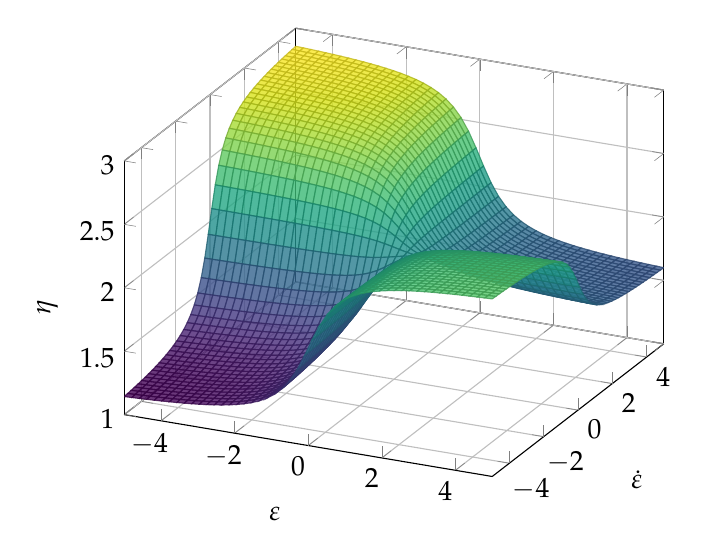
\begin{tikzpicture}
\begin{axis}[zmin=1,zmax=3,grid=major,xtick={-4,-2,...,4},ytick={-4,-2,...,4},ztick={1,1.5,...,3},xlabel=$\varepsilon$,ylabel=$\dot\varepsilon$,zlabel=$\eta$]
\def\ea{1.5}\def\eb{3}\def\ec{1}\def\ed{2.5}\def\ga{1.5}\def\gb{1.5}
\addplot3[opacity=.8,surf,samples=50,colormap name=viridis]{.25*(\ea+\eb+\ec+\ed)+(\ea-\eb+\ec-\ed)/pi/pi*rad(atan(\ga*x))*rad(atan(\gb*y))+(\ea-\eb-\ec+\ed)/pi/2*rad(atan(\ga*x))+(\ea+\eb-\ec-\ed)/pi/2*rad(atan(\gb*y))};
\end{axis}
\end{tikzpicture}
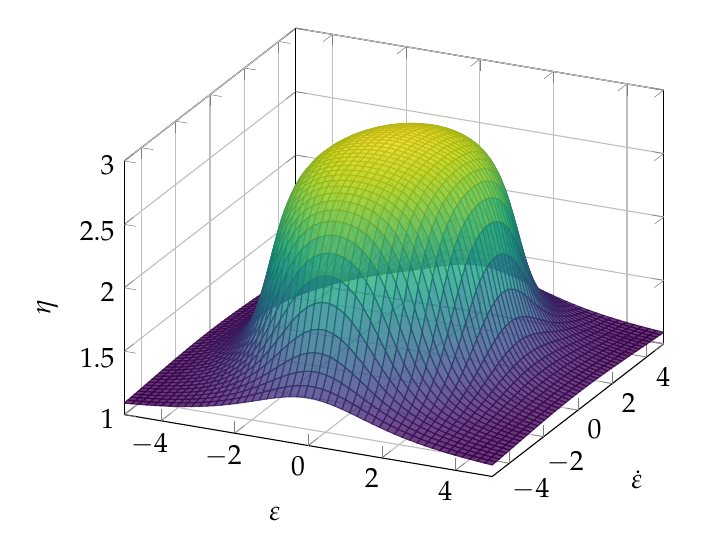
\begin{tikzpicture}
\begin{axis}[zmin=1,zmax=3,grid=major,xtick={-4,-2,...,4},ytick={-4,-2,...,4},ztick={1,1.5,...,3},xlabel=$\varepsilon$,ylabel=$\dot\varepsilon$,zlabel=$\eta$]
\addplot3[opacity=.8,surf,samples=50,colormap name=viridis]{atan(6*(1-.25*sqrt(2*x*x+y*y))))/90+2};
\end{axis}
\end{tikzpicture}
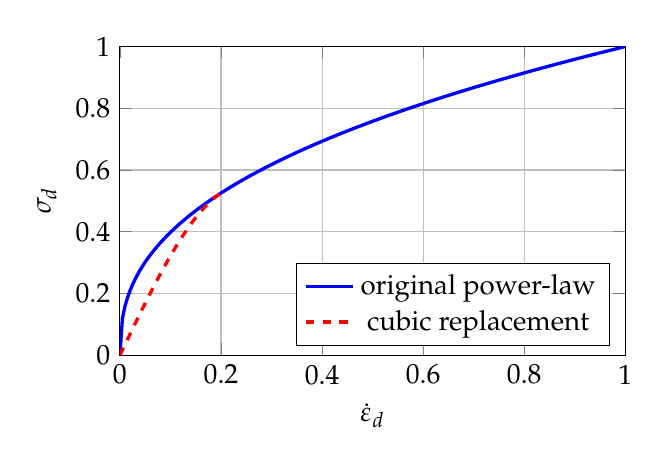
\begin{tikzpicture}
\begin{axis}[width=8cm,height=5.5cm,xmin=0,xmax=1,ymin=0,ymax=1,grid=major,xtick={0,0.2,0.4,0.6,0.8,1.0},ytick={0,0.2,0.4,0.6,0.8,1.0},xlabel=$\dot\varepsilon_d$,ylabel=$\sigma_d$,legend pos=south east]
\addplot[very thick,samples at={0,.005,...,1},blue]{x^.4};
\addplot[dashed,very thick,samples at={0,0.005,...,0.2},red]{-19.699*x^3+3.414*x};
\addlegendentry{original power-law}
\addlegendentry{cubic replacement}
\end{axis}
\end{tikzpicture}
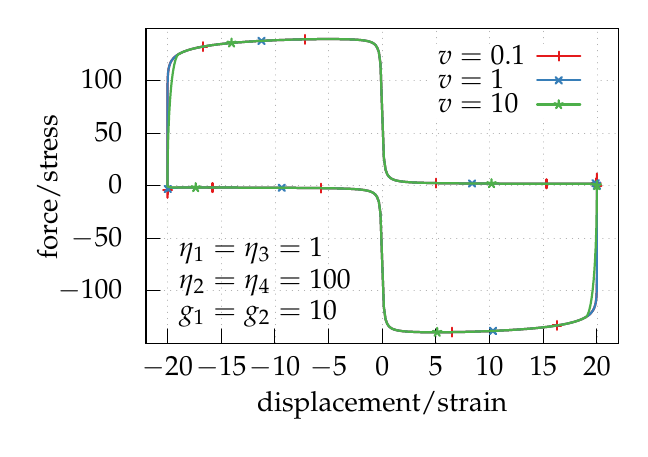
\begin{tikzpicture}[gnuplot]
%% generated with GNUPLOT 5.4p2 (Lua 5.4; terminal rev. Jun 2020, script rev. 114)
%% 11/05/21 19:23:17
\path (0.000,0.000) rectangle (6.000,4.000);
\gpcolor{color=gp lt color axes}
\gpsetlinetype{gp lt axes}
\gpsetdashtype{gp dt axes}
\gpsetlinewidth{0.50}
\draw[gp path] (0.000,0.667)--(5.999,0.667);
\gpcolor{color=gp lt color border}
\gpsetlinetype{gp lt border}
\gpsetdashtype{gp dt solid}
\gpsetlinewidth{1.00}
\draw[gp path] (0.000,0.667)--(0.180,0.667);
\node[gp node right] at (-0.184,0.667) {$-100$};
\gpcolor{color=gp lt color axes}
\gpsetlinetype{gp lt axes}
\gpsetdashtype{gp dt axes}
\gpsetlinewidth{0.50}
\draw[gp path] (0.000,1.333)--(5.999,1.333);
\gpcolor{color=gp lt color border}
\gpsetlinetype{gp lt border}
\gpsetdashtype{gp dt solid}
\gpsetlinewidth{1.00}
\draw[gp path] (0.000,1.333)--(0.180,1.333);
\node[gp node right] at (-0.184,1.333) {$-50$};
\gpcolor{color=gp lt color axes}
\gpsetlinetype{gp lt axes}
\gpsetdashtype{gp dt axes}
\gpsetlinewidth{0.50}
\draw[gp path] (0.000,2.000)--(5.999,2.000);
\gpcolor{color=gp lt color border}
\gpsetlinetype{gp lt border}
\gpsetdashtype{gp dt solid}
\gpsetlinewidth{1.00}
\draw[gp path] (0.000,2.000)--(0.180,2.000);
\node[gp node right] at (-0.184,2.000) {$0$};
\gpcolor{color=gp lt color axes}
\gpsetlinetype{gp lt axes}
\gpsetdashtype{gp dt axes}
\gpsetlinewidth{0.50}
\draw[gp path] (0.000,2.666)--(5.999,2.666);
\gpcolor{color=gp lt color border}
\gpsetlinetype{gp lt border}
\gpsetdashtype{gp dt solid}
\gpsetlinewidth{1.00}
\draw[gp path] (0.000,2.666)--(0.180,2.666);
\node[gp node right] at (-0.184,2.666) {$50$};
\gpcolor{color=gp lt color axes}
\gpsetlinetype{gp lt axes}
\gpsetdashtype{gp dt axes}
\gpsetlinewidth{0.50}
\draw[gp path] (0.000,3.333)--(3.587,3.333);
\draw[gp path] (5.699,3.333)--(5.999,3.333);
\gpcolor{color=gp lt color border}
\gpsetlinetype{gp lt border}
\gpsetdashtype{gp dt solid}
\gpsetlinewidth{1.00}
\draw[gp path] (0.000,3.333)--(0.180,3.333);
\node[gp node right] at (-0.184,3.333) {$100$};
\gpcolor{color=gp lt color axes}
\gpsetlinetype{gp lt axes}
\gpsetdashtype{gp dt axes}
\gpsetlinewidth{0.50}
\draw[gp path] (0.273,0.000)--(0.273,3.999);
\gpcolor{color=gp lt color border}
\gpsetlinetype{gp lt border}
\gpsetdashtype{gp dt solid}
\gpsetlinewidth{1.00}
\draw[gp path] (0.273,0.000)--(0.273,0.180);
\node[gp node center] at (0.273,-0.308) {$-20$};
\gpcolor{color=gp lt color axes}
\gpsetlinetype{gp lt axes}
\gpsetdashtype{gp dt axes}
\gpsetlinewidth{0.50}
\draw[gp path] (0.954,0.000)--(0.954,3.999);
\gpcolor{color=gp lt color border}
\gpsetlinetype{gp lt border}
\gpsetdashtype{gp dt solid}
\gpsetlinewidth{1.00}
\draw[gp path] (0.954,0.000)--(0.954,0.180);
\node[gp node center] at (0.954,-0.308) {$-15$};
\gpcolor{color=gp lt color axes}
\gpsetlinetype{gp lt axes}
\gpsetdashtype{gp dt axes}
\gpsetlinewidth{0.50}
\draw[gp path] (1.636,0.000)--(1.636,3.999);
\gpcolor{color=gp lt color border}
\gpsetlinetype{gp lt border}
\gpsetdashtype{gp dt solid}
\gpsetlinewidth{1.00}
\draw[gp path] (1.636,0.000)--(1.636,0.180);
\node[gp node center] at (1.636,-0.308) {$-10$};
\gpcolor{color=gp lt color axes}
\gpsetlinetype{gp lt axes}
\gpsetdashtype{gp dt axes}
\gpsetlinewidth{0.50}
\draw[gp path] (2.318,0.000)--(2.318,3.999);
\gpcolor{color=gp lt color border}
\gpsetlinetype{gp lt border}
\gpsetdashtype{gp dt solid}
\gpsetlinewidth{1.00}
\draw[gp path] (2.318,0.000)--(2.318,0.180);
\node[gp node center] at (2.318,-0.308) {$-5$};
\gpcolor{color=gp lt color axes}
\gpsetlinetype{gp lt axes}
\gpsetdashtype{gp dt axes}
\gpsetlinewidth{0.50}
\draw[gp path] (3.000,0.000)--(3.000,3.999);
\gpcolor{color=gp lt color border}
\gpsetlinetype{gp lt border}
\gpsetdashtype{gp dt solid}
\gpsetlinewidth{1.00}
\draw[gp path] (3.000,0.000)--(3.000,0.180);
\node[gp node center] at (3.000,-0.308) {$0$};
\gpcolor{color=gp lt color axes}
\gpsetlinetype{gp lt axes}
\gpsetdashtype{gp dt axes}
\gpsetlinewidth{0.50}
\draw[gp path] (3.681,0.000)--(3.681,2.875);
\draw[gp path] (3.681,3.799)--(3.681,3.999);
\gpcolor{color=gp lt color border}
\gpsetlinetype{gp lt border}
\gpsetdashtype{gp dt solid}
\gpsetlinewidth{1.00}
\draw[gp path] (3.681,0.000)--(3.681,0.180);
\node[gp node center] at (3.681,-0.308) {$5$};
\gpcolor{color=gp lt color axes}
\gpsetlinetype{gp lt axes}
\gpsetdashtype{gp dt axes}
\gpsetlinewidth{0.50}
\draw[gp path] (4.363,0.000)--(4.363,2.875);
\draw[gp path] (4.363,3.799)--(4.363,3.999);
\gpcolor{color=gp lt color border}
\gpsetlinetype{gp lt border}
\gpsetdashtype{gp dt solid}
\gpsetlinewidth{1.00}
\draw[gp path] (4.363,0.000)--(4.363,0.180);
\node[gp node center] at (4.363,-0.308) {$10$};
\gpcolor{color=gp lt color axes}
\gpsetlinetype{gp lt axes}
\gpsetdashtype{gp dt axes}
\gpsetlinewidth{0.50}
\draw[gp path] (5.045,0.000)--(5.045,2.875);
\draw[gp path] (5.045,3.799)--(5.045,3.999);
\gpcolor{color=gp lt color border}
\gpsetlinetype{gp lt border}
\gpsetdashtype{gp dt solid}
\gpsetlinewidth{1.00}
\draw[gp path] (5.045,0.000)--(5.045,0.180);
\node[gp node center] at (5.045,-0.308) {$15$};
\gpcolor{color=gp lt color axes}
\gpsetlinetype{gp lt axes}
\gpsetdashtype{gp dt axes}
\gpsetlinewidth{0.50}
\draw[gp path] (5.726,0.000)--(5.726,3.999);
\gpcolor{color=gp lt color border}
\gpsetlinetype{gp lt border}
\gpsetdashtype{gp dt solid}
\gpsetlinewidth{1.00}
\draw[gp path] (5.726,0.000)--(5.726,0.180);
\node[gp node center] at (5.726,-0.308) {$20$};
\draw[gp path] (0.000,3.999)--(0.000,0.000)--(5.999,0.000)--(5.999,3.999)--cycle;
\node[gp node left] at (0.300,1.200) {$\eta_1=\eta_3=1$};
\node[gp node left] at (0.300,0.800) {$\eta_2=\eta_4=100$};
\node[gp node left] at (0.300,0.400) {$g_1=g_2=10$};
\node[gp node center,rotate=-270] at (-1.212,1.999) {force/stress};
\node[gp node center] at (2.999,-0.769) {displacement/strain};
\gpcolor{rgb color={0.894,0.102,0.110}}
\gpsetlinewidth{2.00}
\draw[gp path] (5.726,2.000)--(5.726,0.983)--(5.726,0.837)--(5.726,0.763)--(5.725,0.713)%
  --(5.724,0.675)--(5.723,0.645)--(5.722,0.620)--(5.721,0.598)--(5.720,0.579)--(5.718,0.562)%
  --(5.716,0.546)--(5.714,0.532)--(5.712,0.519)--(5.710,0.507)--(5.707,0.496)--(5.705,0.485)%
  --(5.702,0.475)--(5.699,0.466)--(5.696,0.457)--(5.693,0.449)--(5.689,0.441)--(5.686,0.433)%
  --(5.682,0.426)--(5.678,0.419)--(5.674,0.412)--(5.670,0.406)--(5.665,0.400)--(5.661,0.394)%
  --(5.656,0.388)--(5.651,0.382)--(5.646,0.377)--(5.641,0.372)--(5.635,0.366)--(5.630,0.361)%
  --(5.624,0.357)--(5.618,0.352)--(5.612,0.347)--(5.606,0.343)--(5.599,0.339)--(5.593,0.335)%
  --(5.586,0.330)--(5.579,0.326)--(5.572,0.323)--(5.565,0.319)--(5.558,0.315)--(5.550,0.311)%
  --(5.543,0.308)--(5.535,0.304)--(5.527,0.301)--(5.519,0.298)--(5.510,0.294)--(5.502,0.291)%
  --(5.493,0.288)--(5.485,0.285)--(5.476,0.282)--(5.467,0.279)--(5.458,0.276)--(5.448,0.273)%
  --(5.439,0.270)--(5.429,0.268)--(5.419,0.265)--(5.409,0.262)--(5.399,0.260)--(5.389,0.257)%
  --(5.379,0.255)--(5.368,0.252)--(5.357,0.250)--(5.347,0.247)--(5.336,0.245)--(5.324,0.243)%
  --(5.313,0.240)--(5.302,0.238)--(5.290,0.236)--(5.279,0.234)--(5.267,0.232)--(5.255,0.230)%
  --(5.243,0.228)--(5.230,0.226)--(5.218,0.224)--(5.206,0.222)--(5.193,0.220)--(5.180,0.218)%
  --(5.167,0.216)--(5.154,0.214)--(5.141,0.212)--(5.128,0.211)--(5.114,0.209)--(5.101,0.207)%
  --(5.087,0.205)--(5.073,0.204)--(5.059,0.202)--(5.045,0.201)--(5.031,0.199)--(5.016,0.197)%
  --(5.002,0.196)--(4.987,0.194)--(4.973,0.193)--(4.958,0.191)--(4.943,0.190)--(4.928,0.189)%
  --(4.912,0.187)--(4.897,0.186)--(4.882,0.184)--(4.866,0.183)--(4.850,0.182)--(4.835,0.180)%
  --(4.819,0.179)--(4.803,0.178)--(4.787,0.177)--(4.770,0.176)--(4.754,0.174)--(4.738,0.173)%
  --(4.721,0.172)--(4.704,0.171)--(4.688,0.170)--(4.671,0.169)--(4.654,0.168)--(4.637,0.167)%
  --(4.620,0.166)--(4.602,0.164)--(4.585,0.163)--(4.567,0.163)--(4.550,0.162)--(4.532,0.161)%
  --(4.514,0.160)--(4.497,0.159)--(4.479,0.158)--(4.461,0.157)--(4.442,0.156)--(4.424,0.155)%
  --(4.406,0.155)--(4.388,0.154)--(4.369,0.153)--(4.351,0.152)--(4.332,0.151)--(4.313,0.151)%
  --(4.294,0.150)--(4.275,0.149)--(4.256,0.149)--(4.237,0.148)--(4.218,0.147)--(4.199,0.147)%
  --(4.180,0.146)--(4.161,0.145)--(4.141,0.145)--(4.122,0.144)--(4.102,0.144)--(4.082,0.143)%
  --(4.063,0.143)--(4.043,0.142)--(4.023,0.142)--(4.003,0.141)--(3.983,0.141)--(3.963,0.141)%
  --(3.943,0.140)--(3.923,0.140)--(3.903,0.140)--(3.883,0.139)--(3.862,0.139)--(3.842,0.139)%
  --(3.822,0.138)--(3.801,0.138)--(3.781,0.138)--(3.760,0.138)--(3.740,0.138)--(3.719,0.138)%
  --(3.698,0.138)--(3.678,0.138)--(3.657,0.138)--(3.636,0.138)--(3.615,0.138)--(3.594,0.138)%
  --(3.573,0.138)--(3.552,0.138)--(3.531,0.139)--(3.510,0.139)--(3.489,0.139)--(3.468,0.140)%
  --(3.447,0.140)--(3.426,0.141)--(3.405,0.142)--(3.384,0.143)--(3.362,0.144)--(3.341,0.145)%
  --(3.320,0.146)--(3.299,0.148)--(3.277,0.150)--(3.256,0.152)--(3.235,0.155)--(3.213,0.158)%
  --(3.192,0.162)--(3.171,0.167)--(3.149,0.174)--(3.128,0.182)--(3.107,0.195)--(3.085,0.213)%
  --(3.064,0.244)--(3.042,0.302)--(3.021,0.455)--(2.999,1.049)--(2.978,1.643)--(2.957,1.796)%
  --(2.935,1.855)--(2.914,1.885)--(2.892,1.904)--(2.871,1.916)--(2.850,1.925)--(2.828,1.932)%
  --(2.807,1.937)--(2.786,1.941)--(2.764,1.945)--(2.743,1.947)--(2.722,1.950)--(2.700,1.952)%
  --(2.679,1.954)--(2.658,1.955)--(2.637,1.957)--(2.615,1.958)--(2.594,1.959)--(2.573,1.960)%
  --(2.552,1.961)--(2.531,1.962)--(2.510,1.962)--(2.489,1.963)--(2.468,1.964)--(2.447,1.964)%
  --(2.426,1.965)--(2.405,1.965)--(2.384,1.966)--(2.363,1.966)--(2.342,1.967)--(2.321,1.967)%
  --(2.301,1.967)--(2.280,1.968)--(2.259,1.968)--(2.239,1.968)--(2.218,1.969)--(2.198,1.969)%
  --(2.177,1.969)--(2.157,1.969)--(2.137,1.970)--(2.116,1.970)--(2.096,1.970)--(2.076,1.970)%
  --(2.056,1.970)--(2.036,1.970)--(2.016,1.971)--(1.996,1.971)--(1.976,1.971)--(1.956,1.971)%
  --(1.936,1.971)--(1.917,1.971)--(1.897,1.972)--(1.877,1.972)--(1.858,1.972)--(1.838,1.972)%
  --(1.819,1.972)--(1.800,1.972)--(1.781,1.972)--(1.762,1.972)--(1.743,1.972)--(1.724,1.973)%
  --(1.705,1.973)--(1.686,1.973)--(1.667,1.973)--(1.648,1.973)--(1.630,1.973)--(1.611,1.973)%
  --(1.593,1.973)--(1.575,1.973)--(1.557,1.973)--(1.538,1.973)--(1.520,1.973)--(1.502,1.974)%
  --(1.485,1.974)--(1.467,1.974)--(1.449,1.974)--(1.432,1.974)--(1.414,1.974)--(1.397,1.974)%
  --(1.379,1.974)--(1.362,1.974)--(1.345,1.974)--(1.328,1.974)--(1.311,1.974)--(1.295,1.974)%
  --(1.278,1.974)--(1.261,1.974)--(1.245,1.974)--(1.229,1.974)--(1.212,1.974)--(1.196,1.974)%
  --(1.180,1.974)--(1.164,1.975)--(1.149,1.975)--(1.133,1.975)--(1.117,1.975)--(1.102,1.975)%
  --(1.087,1.975)--(1.071,1.975)--(1.056,1.975)--(1.041,1.975)--(1.026,1.975)--(1.012,1.975)%
  --(0.997,1.975)--(0.983,1.975)--(0.968,1.975)--(0.954,1.975)--(0.940,1.975)--(0.926,1.975)%
  --(0.912,1.975)--(0.898,1.975)--(0.885,1.975)--(0.871,1.975)--(0.858,1.975)--(0.845,1.975)%
  --(0.832,1.975)--(0.819,1.975)--(0.806,1.975)--(0.793,1.975)--(0.781,1.975)--(0.769,1.975)%
  --(0.756,1.975)--(0.744,1.975)--(0.732,1.975)--(0.720,1.975)--(0.709,1.975)--(0.697,1.975)%
  --(0.686,1.975)--(0.675,1.975)--(0.663,1.975)--(0.652,1.975)--(0.642,1.975)--(0.631,1.975)%
  --(0.620,1.975)--(0.610,1.975)--(0.600,1.975)--(0.590,1.975)--(0.580,1.975)--(0.570,1.975)%
  --(0.560,1.975)--(0.551,1.975)--(0.541,1.975)--(0.532,1.975)--(0.523,1.975)--(0.514,1.975)%
  --(0.506,1.975)--(0.497,1.975)--(0.489,1.975)--(0.480,1.975)--(0.472,1.975)--(0.464,1.975)%
  --(0.456,1.975)--(0.449,1.975)--(0.441,1.975)--(0.434,1.975)--(0.427,1.975)--(0.420,1.975)%
  --(0.413,1.975)--(0.406,1.975)--(0.400,1.975)--(0.393,1.974)--(0.387,1.974)--(0.381,1.974)%
  --(0.375,1.974)--(0.369,1.974)--(0.364,1.974)--(0.358,1.974)--(0.353,1.974)--(0.348,1.974)%
  --(0.343,1.973)--(0.338,1.973)--(0.334,1.973)--(0.329,1.973)--(0.325,1.973)--(0.321,1.973)%
  --(0.317,1.972)--(0.313,1.972)--(0.310,1.972)--(0.306,1.971)--(0.303,1.971)--(0.300,1.971)%
  --(0.297,1.970)--(0.294,1.970)--(0.292,1.969)--(0.289,1.968)--(0.287,1.967)--(0.285,1.967)%
  --(0.283,1.965)--(0.281,1.964)--(0.279,1.962)--(0.278,1.960)--(0.277,1.958)--(0.276,1.954)%
  --(0.275,1.949)--(0.274,1.942)--(0.273,1.930)--(0.273,1.907)--(0.273,1.846)--(0.273,2.000)%
  --(0.273,3.016)--(0.273,3.162)--(0.273,3.236)--(0.274,3.286)--(0.275,3.324)--(0.276,3.354)%
  --(0.277,3.379)--(0.278,3.401)--(0.279,3.420)--(0.281,3.437)--(0.283,3.453)--(0.285,3.467)%
  --(0.287,3.480)--(0.289,3.492)--(0.292,3.503)--(0.294,3.514)--(0.297,3.524)--(0.300,3.533)%
  --(0.303,3.542)--(0.306,3.550)--(0.310,3.558)--(0.313,3.566)--(0.317,3.573)--(0.321,3.580)%
  --(0.325,3.587)--(0.329,3.593)--(0.334,3.599)--(0.338,3.605)--(0.343,3.611)--(0.348,3.617)%
  --(0.353,3.622)--(0.358,3.627)--(0.364,3.633)--(0.369,3.638)--(0.375,3.642)--(0.381,3.647)%
  --(0.387,3.652)--(0.393,3.656)--(0.400,3.660)--(0.406,3.664)--(0.413,3.669)--(0.420,3.673)%
  --(0.427,3.676)--(0.434,3.680)--(0.441,3.684)--(0.449,3.688)--(0.456,3.691)--(0.464,3.695)%
  --(0.472,3.698)--(0.480,3.701)--(0.489,3.705)--(0.497,3.708)--(0.506,3.711)--(0.514,3.714)%
  --(0.523,3.717)--(0.532,3.720)--(0.541,3.723)--(0.551,3.726)--(0.560,3.729)--(0.570,3.731)%
  --(0.580,3.734)--(0.590,3.737)--(0.600,3.739)--(0.610,3.742)--(0.620,3.744)--(0.631,3.747)%
  --(0.642,3.749)--(0.652,3.752)--(0.663,3.754)--(0.675,3.756)--(0.686,3.759)--(0.697,3.761)%
  --(0.709,3.763)--(0.720,3.765)--(0.732,3.767)--(0.744,3.769)--(0.756,3.771)--(0.769,3.773)%
  --(0.781,3.775)--(0.793,3.777)--(0.806,3.779)--(0.819,3.781)--(0.832,3.783)--(0.845,3.785)%
  --(0.858,3.787)--(0.871,3.788)--(0.885,3.790)--(0.898,3.792)--(0.912,3.794)--(0.926,3.795)%
  --(0.940,3.797)--(0.954,3.798)--(0.968,3.800)--(0.983,3.802)--(0.997,3.803)--(1.012,3.805)%
  --(1.026,3.806)--(1.041,3.808)--(1.056,3.809)--(1.071,3.810)--(1.087,3.812)--(1.102,3.813)%
  --(1.117,3.815)--(1.133,3.816)--(1.149,3.817)--(1.164,3.819)--(1.180,3.820)--(1.196,3.821)%
  --(1.212,3.822)--(1.229,3.823)--(1.245,3.825)--(1.261,3.826)--(1.278,3.827)--(1.295,3.828)%
  --(1.311,3.829)--(1.328,3.830)--(1.345,3.831)--(1.362,3.832)--(1.379,3.833)--(1.397,3.835)%
  --(1.414,3.836)--(1.432,3.836)--(1.449,3.837)--(1.467,3.838)--(1.485,3.839)--(1.502,3.840)%
  --(1.520,3.841)--(1.538,3.842)--(1.557,3.843)--(1.575,3.844)--(1.593,3.844)--(1.611,3.845)%
  --(1.630,3.846)--(1.648,3.847)--(1.667,3.848)--(1.686,3.848)--(1.705,3.849)--(1.724,3.850)%
  --(1.743,3.850)--(1.762,3.851)--(1.781,3.852)--(1.800,3.852)--(1.819,3.853)--(1.838,3.854)%
  --(1.858,3.854)--(1.877,3.855)--(1.897,3.855)--(1.917,3.856)--(1.936,3.856)--(1.956,3.857)%
  --(1.976,3.857)--(1.996,3.858)--(2.016,3.858)--(2.036,3.858)--(2.056,3.859)--(2.076,3.859)%
  --(2.096,3.859)--(2.116,3.860)--(2.137,3.860)--(2.157,3.860)--(2.177,3.861)--(2.198,3.861)%
  --(2.218,3.861)--(2.239,3.861)--(2.259,3.861)--(2.280,3.861)--(2.301,3.861)--(2.321,3.861)%
  --(2.342,3.861)--(2.363,3.861)--(2.384,3.861)--(2.405,3.861)--(2.426,3.861)--(2.447,3.861)%
  --(2.468,3.860)--(2.489,3.860)--(2.510,3.860)--(2.531,3.859)--(2.552,3.859)--(2.573,3.858)%
  --(2.594,3.857)--(2.615,3.856)--(2.637,3.855)--(2.658,3.854)--(2.679,3.853)--(2.700,3.851)%
  --(2.722,3.849)--(2.743,3.847)--(2.764,3.844)--(2.786,3.841)--(2.807,3.837)--(2.828,3.832)%
  --(2.850,3.825)--(2.871,3.817)--(2.892,3.804)--(2.914,3.786)--(2.935,3.755)--(2.957,3.697)%
  --(2.978,3.544)--(2.999,2.950)--(3.021,2.356)--(3.042,2.203)--(3.064,2.144)--(3.085,2.114)%
  --(3.107,2.095)--(3.128,2.083)--(3.149,2.074)--(3.171,2.067)--(3.192,2.062)--(3.213,2.058)%
  --(3.235,2.054)--(3.256,2.052)--(3.277,2.049)--(3.299,2.047)--(3.320,2.045)--(3.341,2.044)%
  --(3.362,2.042)--(3.384,2.041)--(3.405,2.040)--(3.426,2.039)--(3.447,2.038)--(3.468,2.037)%
  --(3.489,2.037)--(3.510,2.036)--(3.531,2.035)--(3.552,2.035)--(3.573,2.034)--(3.594,2.034)%
  --(3.615,2.033)--(3.636,2.033)--(3.657,2.032)--(3.678,2.032)--(3.698,2.032)--(3.719,2.031)%
  --(3.740,2.031)--(3.760,2.031)--(3.781,2.030)--(3.801,2.030)--(3.822,2.030)--(3.842,2.030)%
  --(3.862,2.029)--(3.883,2.029)--(3.903,2.029)--(3.923,2.029)--(3.943,2.029)--(3.963,2.029)%
  --(3.983,2.028)--(4.003,2.028)--(4.023,2.028)--(4.043,2.028)--(4.063,2.028)--(4.082,2.028)%
  --(4.102,2.027)--(4.122,2.027)--(4.141,2.027)--(4.161,2.027)--(4.180,2.027)--(4.199,2.027)%
  --(4.218,2.027)--(4.237,2.027)--(4.256,2.027)--(4.275,2.026)--(4.294,2.026)--(4.313,2.026)%
  --(4.332,2.026)--(4.351,2.026)--(4.369,2.026)--(4.388,2.026)--(4.406,2.026)--(4.424,2.026)%
  --(4.442,2.026)--(4.461,2.026)--(4.479,2.026)--(4.497,2.025)--(4.514,2.025)--(4.532,2.025)%
  --(4.550,2.025)--(4.567,2.025)--(4.585,2.025)--(4.602,2.025)--(4.620,2.025)--(4.637,2.025)%
  --(4.654,2.025)--(4.671,2.025)--(4.688,2.025)--(4.704,2.025)--(4.721,2.025)--(4.738,2.025)%
  --(4.754,2.025)--(4.770,2.025)--(4.787,2.025)--(4.803,2.025)--(4.819,2.025)--(4.835,2.024)%
  --(4.850,2.024)--(4.866,2.024)--(4.882,2.024)--(4.897,2.024)--(4.912,2.024)--(4.928,2.024)%
  --(4.943,2.024)--(4.958,2.024)--(4.973,2.024)--(4.987,2.024)--(5.002,2.024)--(5.016,2.024)%
  --(5.031,2.024)--(5.045,2.024)--(5.059,2.024)--(5.073,2.024)--(5.087,2.024)--(5.101,2.024)%
  --(5.114,2.024)--(5.128,2.024)--(5.141,2.024)--(5.154,2.024)--(5.167,2.024)--(5.180,2.024)%
  --(5.193,2.024)--(5.206,2.024)--(5.218,2.024)--(5.230,2.024)--(5.243,2.024)--(5.255,2.024)%
  --(5.267,2.024)--(5.279,2.024)--(5.290,2.024)--(5.302,2.024)--(5.313,2.024)--(5.324,2.024)%
  --(5.336,2.024)--(5.347,2.024)--(5.357,2.024)--(5.368,2.024)--(5.379,2.024)--(5.389,2.024)%
  --(5.399,2.024)--(5.409,2.024)--(5.419,2.024)--(5.429,2.024)--(5.439,2.024)--(5.448,2.024)%
  --(5.458,2.024)--(5.467,2.024)--(5.476,2.024)--(5.485,2.024)--(5.493,2.024)--(5.502,2.024)%
  --(5.510,2.024)--(5.519,2.024)--(5.527,2.024)--(5.535,2.024)--(5.543,2.024)--(5.550,2.024)%
  --(5.558,2.024)--(5.565,2.024)--(5.572,2.024)--(5.579,2.024)--(5.586,2.024)--(5.593,2.024)%
  --(5.599,2.024)--(5.606,2.025)--(5.612,2.025)--(5.618,2.025)--(5.624,2.025)--(5.630,2.025)%
  --(5.635,2.025)--(5.641,2.025)--(5.646,2.025)--(5.651,2.025)--(5.656,2.026)--(5.661,2.026)%
  --(5.665,2.026)--(5.670,2.026)--(5.674,2.026)--(5.678,2.026)--(5.682,2.027)--(5.686,2.027)%
  --(5.689,2.027)--(5.693,2.028)--(5.696,2.028)--(5.699,2.028)--(5.702,2.029)--(5.705,2.029)%
  --(5.707,2.030)--(5.710,2.031)--(5.712,2.032)--(5.714,2.032)--(5.716,2.034)--(5.718,2.035)%
  --(5.720,2.037)--(5.721,2.039)--(5.722,2.041)--(5.723,2.045)--(5.724,2.050)--(5.725,2.057)%
  --(5.726,2.069)--(5.726,2.092)--(5.726,2.153)--cycle;
\gpsetpointsize{4.00}
\gp3point{gp mark 1}{}{(5.726,2.000)}
\gp3point{gp mark 1}{}{(5.218,0.224)}
\gp3point{gp mark 1}{}{(3.883,0.139)}
\gp3point{gp mark 1}{}{(2.218,1.969)}
\gp3point{gp mark 1}{}{(0.845,1.975)}
\gp3point{gp mark 1}{}{(0.275,1.949)}
\gp3point{gp mark 1}{}{(0.720,3.765)}
\gp3point{gp mark 1}{}{(2.016,3.858)}
\gp3point{gp mark 1}{}{(3.678,2.032)}
\gp3point{gp mark 1}{}{(5.087,2.024)}
\gp3point{gp mark 1}{}{(5.718,2.035)}
\gpcolor{rgb color={0.216,0.494,0.722}}
\draw[gp path] (5.726,2.000)--(5.726,1.589)--(5.726,1.175)--(5.726,0.864)--(5.725,0.713)%
  --(5.724,0.675)--(5.723,0.645)--(5.722,0.620)--(5.721,0.598)--(5.720,0.579)--(5.718,0.562)%
  --(5.716,0.546)--(5.714,0.532)--(5.712,0.519)--(5.710,0.507)--(5.707,0.496)--(5.705,0.485)%
  --(5.702,0.475)--(5.699,0.466)--(5.696,0.457)--(5.693,0.449)--(5.689,0.441)--(5.686,0.433)%
  --(5.682,0.426)--(5.678,0.419)--(5.674,0.412)--(5.670,0.406)--(5.665,0.400)--(5.661,0.394)%
  --(5.656,0.388)--(5.651,0.382)--(5.646,0.377)--(5.641,0.372)--(5.635,0.366)--(5.630,0.361)%
  --(5.624,0.357)--(5.618,0.352)--(5.612,0.347)--(5.606,0.343)--(5.599,0.339)--(5.593,0.335)%
  --(5.586,0.330)--(5.579,0.326)--(5.572,0.323)--(5.565,0.319)--(5.558,0.315)--(5.550,0.311)%
  --(5.543,0.308)--(5.535,0.304)--(5.527,0.301)--(5.519,0.298)--(5.510,0.294)--(5.502,0.291)%
  --(5.493,0.288)--(5.485,0.285)--(5.476,0.282)--(5.467,0.279)--(5.458,0.276)--(5.448,0.273)%
  --(5.439,0.270)--(5.429,0.268)--(5.419,0.265)--(5.409,0.262)--(5.399,0.260)--(5.389,0.257)%
  --(5.379,0.255)--(5.368,0.252)--(5.357,0.250)--(5.347,0.247)--(5.336,0.245)--(5.324,0.243)%
  --(5.313,0.240)--(5.302,0.238)--(5.290,0.236)--(5.279,0.234)--(5.267,0.232)--(5.255,0.230)%
  --(5.243,0.228)--(5.230,0.226)--(5.218,0.224)--(5.206,0.222)--(5.193,0.220)--(5.180,0.218)%
  --(5.167,0.216)--(5.154,0.214)--(5.141,0.212)--(5.128,0.211)--(5.114,0.209)--(5.101,0.207)%
  --(5.087,0.205)--(5.073,0.204)--(5.059,0.202)--(5.045,0.201)--(5.031,0.199)--(5.016,0.197)%
  --(5.002,0.196)--(4.987,0.194)--(4.973,0.193)--(4.958,0.191)--(4.943,0.190)--(4.928,0.189)%
  --(4.912,0.187)--(4.897,0.186)--(4.882,0.184)--(4.866,0.183)--(4.850,0.182)--(4.835,0.180)%
  --(4.819,0.179)--(4.803,0.178)--(4.787,0.177)--(4.770,0.176)--(4.754,0.174)--(4.738,0.173)%
  --(4.721,0.172)--(4.704,0.171)--(4.688,0.170)--(4.671,0.169)--(4.654,0.168)--(4.637,0.167)%
  --(4.620,0.166)--(4.602,0.164)--(4.585,0.163)--(4.567,0.163)--(4.550,0.162)--(4.532,0.161)%
  --(4.514,0.160)--(4.497,0.159)--(4.479,0.158)--(4.461,0.157)--(4.442,0.156)--(4.424,0.155)%
  --(4.406,0.155)--(4.388,0.154)--(4.369,0.153)--(4.351,0.152)--(4.332,0.151)--(4.313,0.151)%
  --(4.294,0.150)--(4.275,0.149)--(4.256,0.149)--(4.237,0.148)--(4.218,0.147)--(4.199,0.147)%
  --(4.180,0.146)--(4.161,0.145)--(4.141,0.145)--(4.122,0.144)--(4.102,0.144)--(4.082,0.143)%
  --(4.063,0.143)--(4.043,0.142)--(4.023,0.142)--(4.003,0.141)--(3.983,0.141)--(3.963,0.141)%
  --(3.943,0.140)--(3.923,0.140)--(3.903,0.140)--(3.883,0.139)--(3.862,0.139)--(3.842,0.139)%
  --(3.822,0.138)--(3.801,0.138)--(3.781,0.138)--(3.760,0.138)--(3.740,0.138)--(3.719,0.138)%
  --(3.698,0.138)--(3.678,0.138)--(3.657,0.138)--(3.636,0.138)--(3.615,0.138)--(3.594,0.138)%
  --(3.573,0.138)--(3.552,0.138)--(3.531,0.139)--(3.510,0.139)--(3.489,0.139)--(3.468,0.140)%
  --(3.447,0.140)--(3.426,0.141)--(3.405,0.142)--(3.384,0.143)--(3.362,0.144)--(3.341,0.145)%
  --(3.320,0.146)--(3.299,0.148)--(3.277,0.150)--(3.256,0.152)--(3.235,0.155)--(3.213,0.158)%
  --(3.192,0.162)--(3.171,0.167)--(3.149,0.174)--(3.128,0.182)--(3.107,0.195)--(3.085,0.213)%
  --(3.064,0.244)--(3.042,0.302)--(3.021,0.455)--(2.999,1.049)--(2.978,1.643)--(2.957,1.796)%
  --(2.935,1.855)--(2.914,1.885)--(2.892,1.904)--(2.871,1.916)--(2.850,1.925)--(2.828,1.932)%
  --(2.807,1.937)--(2.786,1.941)--(2.764,1.945)--(2.743,1.947)--(2.722,1.950)--(2.700,1.952)%
  --(2.679,1.954)--(2.658,1.955)--(2.637,1.957)--(2.615,1.958)--(2.594,1.959)--(2.573,1.960)%
  --(2.552,1.961)--(2.531,1.962)--(2.510,1.962)--(2.489,1.963)--(2.468,1.964)--(2.447,1.964)%
  --(2.426,1.965)--(2.405,1.965)--(2.384,1.966)--(2.363,1.966)--(2.342,1.967)--(2.321,1.967)%
  --(2.301,1.967)--(2.280,1.968)--(2.259,1.968)--(2.239,1.968)--(2.218,1.969)--(2.198,1.969)%
  --(2.177,1.969)--(2.157,1.969)--(2.137,1.970)--(2.116,1.970)--(2.096,1.970)--(2.076,1.970)%
  --(2.056,1.970)--(2.036,1.970)--(2.016,1.971)--(1.996,1.971)--(1.976,1.971)--(1.956,1.971)%
  --(1.936,1.971)--(1.917,1.971)--(1.897,1.972)--(1.877,1.972)--(1.858,1.972)--(1.838,1.972)%
  --(1.819,1.972)--(1.800,1.972)--(1.781,1.972)--(1.762,1.972)--(1.743,1.972)--(1.724,1.973)%
  --(1.705,1.973)--(1.686,1.973)--(1.667,1.973)--(1.648,1.973)--(1.630,1.973)--(1.611,1.973)%
  --(1.593,1.973)--(1.575,1.973)--(1.557,1.973)--(1.538,1.973)--(1.520,1.973)--(1.502,1.974)%
  --(1.485,1.974)--(1.467,1.974)--(1.449,1.974)--(1.432,1.974)--(1.414,1.974)--(1.397,1.974)%
  --(1.379,1.974)--(1.362,1.974)--(1.345,1.974)--(1.328,1.974)--(1.311,1.974)--(1.295,1.974)%
  --(1.278,1.974)--(1.261,1.974)--(1.245,1.974)--(1.229,1.974)--(1.212,1.974)--(1.196,1.974)%
  --(1.180,1.974)--(1.164,1.975)--(1.149,1.975)--(1.133,1.975)--(1.117,1.975)--(1.102,1.975)%
  --(1.087,1.975)--(1.071,1.975)--(1.056,1.975)--(1.041,1.975)--(1.026,1.975)--(1.012,1.975)%
  --(0.997,1.975)--(0.983,1.975)--(0.968,1.975)--(0.954,1.975)--(0.940,1.975)--(0.926,1.975)%
  --(0.912,1.975)--(0.898,1.975)--(0.885,1.975)--(0.871,1.975)--(0.858,1.975)--(0.845,1.975)%
  --(0.832,1.975)--(0.819,1.975)--(0.806,1.975)--(0.793,1.975)--(0.781,1.975)--(0.769,1.975)%
  --(0.756,1.975)--(0.744,1.975)--(0.732,1.975)--(0.720,1.975)--(0.709,1.975)--(0.697,1.975)%
  --(0.686,1.975)--(0.675,1.975)--(0.663,1.975)--(0.652,1.975)--(0.642,1.975)--(0.631,1.975)%
  --(0.620,1.975)--(0.610,1.975)--(0.600,1.975)--(0.590,1.975)--(0.580,1.975)--(0.570,1.975)%
  --(0.560,1.975)--(0.551,1.975)--(0.541,1.975)--(0.532,1.975)--(0.523,1.975)--(0.514,1.975)%
  --(0.506,1.975)--(0.497,1.975)--(0.489,1.975)--(0.480,1.975)--(0.472,1.975)--(0.464,1.975)%
  --(0.456,1.975)--(0.449,1.975)--(0.441,1.975)--(0.434,1.975)--(0.427,1.975)--(0.420,1.975)%
  --(0.413,1.975)--(0.406,1.975)--(0.400,1.975)--(0.393,1.974)--(0.387,1.974)--(0.381,1.974)%
  --(0.375,1.974)--(0.369,1.974)--(0.364,1.974)--(0.358,1.974)--(0.353,1.974)--(0.348,1.974)%
  --(0.343,1.973)--(0.338,1.973)--(0.334,1.973)--(0.329,1.973)--(0.325,1.973)--(0.321,1.973)%
  --(0.317,1.972)--(0.313,1.972)--(0.310,1.972)--(0.306,1.971)--(0.303,1.971)--(0.300,1.971)%
  --(0.297,1.970)--(0.294,1.970)--(0.292,1.969)--(0.289,1.968)--(0.287,1.967)--(0.285,1.967)%
  --(0.283,1.965)--(0.281,1.964)--(0.279,1.962)--(0.278,1.960)--(0.277,1.958)--(0.276,1.954)%
  --(0.275,1.949)--(0.274,1.942)--(0.273,1.936)--(0.273,1.934)--(0.273,1.937)--(0.273,2.000)%
  --(0.273,2.410)--(0.273,2.824)--(0.273,3.135)--(0.274,3.286)--(0.275,3.324)--(0.276,3.354)%
  --(0.277,3.379)--(0.278,3.401)--(0.279,3.420)--(0.281,3.437)--(0.283,3.453)--(0.285,3.467)%
  --(0.287,3.480)--(0.289,3.492)--(0.292,3.503)--(0.294,3.514)--(0.297,3.524)--(0.300,3.533)%
  --(0.303,3.542)--(0.306,3.550)--(0.310,3.558)--(0.313,3.566)--(0.317,3.573)--(0.321,3.580)%
  --(0.325,3.587)--(0.329,3.593)--(0.334,3.599)--(0.338,3.605)--(0.343,3.611)--(0.348,3.617)%
  --(0.353,3.622)--(0.358,3.627)--(0.364,3.633)--(0.369,3.638)--(0.375,3.642)--(0.381,3.647)%
  --(0.387,3.652)--(0.393,3.656)--(0.400,3.660)--(0.406,3.664)--(0.413,3.669)--(0.420,3.673)%
  --(0.427,3.676)--(0.434,3.680)--(0.441,3.684)--(0.449,3.688)--(0.456,3.691)--(0.464,3.695)%
  --(0.472,3.698)--(0.480,3.701)--(0.489,3.705)--(0.497,3.708)--(0.506,3.711)--(0.514,3.714)%
  --(0.523,3.717)--(0.532,3.720)--(0.541,3.723)--(0.551,3.726)--(0.560,3.729)--(0.570,3.731)%
  --(0.580,3.734)--(0.590,3.737)--(0.600,3.739)--(0.610,3.742)--(0.620,3.744)--(0.631,3.747)%
  --(0.642,3.749)--(0.652,3.752)--(0.663,3.754)--(0.675,3.756)--(0.686,3.759)--(0.697,3.761)%
  --(0.709,3.763)--(0.720,3.765)--(0.732,3.767)--(0.744,3.769)--(0.756,3.771)--(0.769,3.773)%
  --(0.781,3.775)--(0.793,3.777)--(0.806,3.779)--(0.819,3.781)--(0.832,3.783)--(0.845,3.785)%
  --(0.858,3.787)--(0.871,3.788)--(0.885,3.790)--(0.898,3.792)--(0.912,3.794)--(0.926,3.795)%
  --(0.940,3.797)--(0.954,3.798)--(0.968,3.800)--(0.983,3.802)--(0.997,3.803)--(1.012,3.805)%
  --(1.026,3.806)--(1.041,3.808)--(1.056,3.809)--(1.071,3.810)--(1.087,3.812)--(1.102,3.813)%
  --(1.117,3.815)--(1.133,3.816)--(1.149,3.817)--(1.164,3.819)--(1.180,3.820)--(1.196,3.821)%
  --(1.212,3.822)--(1.229,3.823)--(1.245,3.825)--(1.261,3.826)--(1.278,3.827)--(1.295,3.828)%
  --(1.311,3.829)--(1.328,3.830)--(1.345,3.831)--(1.362,3.832)--(1.379,3.833)--(1.397,3.835)%
  --(1.414,3.836)--(1.432,3.836)--(1.449,3.837)--(1.467,3.838)--(1.485,3.839)--(1.502,3.840)%
  --(1.520,3.841)--(1.538,3.842)--(1.557,3.843)--(1.575,3.844)--(1.593,3.844)--(1.611,3.845)%
  --(1.630,3.846)--(1.648,3.847)--(1.667,3.848)--(1.686,3.848)--(1.705,3.849)--(1.724,3.850)%
  --(1.743,3.850)--(1.762,3.851)--(1.781,3.852)--(1.800,3.852)--(1.819,3.853)--(1.838,3.854)%
  --(1.858,3.854)--(1.877,3.855)--(1.897,3.855)--(1.917,3.856)--(1.936,3.856)--(1.956,3.857)%
  --(1.976,3.857)--(1.996,3.858)--(2.016,3.858)--(2.036,3.858)--(2.056,3.859)--(2.076,3.859)%
  --(2.096,3.859)--(2.116,3.860)--(2.137,3.860)--(2.157,3.860)--(2.177,3.861)--(2.198,3.861)%
  --(2.218,3.861)--(2.239,3.861)--(2.259,3.861)--(2.280,3.861)--(2.301,3.861)--(2.321,3.861)%
  --(2.342,3.861)--(2.363,3.861)--(2.384,3.861)--(2.405,3.861)--(2.426,3.861)--(2.447,3.861)%
  --(2.468,3.860)--(2.489,3.860)--(2.510,3.860)--(2.531,3.859)--(2.552,3.859)--(2.573,3.858)%
  --(2.594,3.857)--(2.615,3.856)--(2.637,3.855)--(2.658,3.854)--(2.679,3.853)--(2.700,3.851)%
  --(2.722,3.849)--(2.743,3.847)--(2.764,3.844)--(2.786,3.841)--(2.807,3.837)--(2.828,3.832)%
  --(2.850,3.825)--(2.871,3.817)--(2.892,3.804)--(2.914,3.786)--(2.935,3.755)--(2.957,3.697)%
  --(2.978,3.544)--(2.999,2.950)--(3.021,2.356)--(3.042,2.203)--(3.064,2.144)--(3.085,2.114)%
  --(3.107,2.095)--(3.128,2.083)--(3.149,2.074)--(3.171,2.067)--(3.192,2.062)--(3.213,2.058)%
  --(3.235,2.054)--(3.256,2.052)--(3.277,2.049)--(3.299,2.047)--(3.320,2.045)--(3.341,2.044)%
  --(3.362,2.042)--(3.384,2.041)--(3.405,2.040)--(3.426,2.039)--(3.447,2.038)--(3.468,2.037)%
  --(3.489,2.037)--(3.510,2.036)--(3.531,2.035)--(3.552,2.035)--(3.573,2.034)--(3.594,2.034)%
  --(3.615,2.033)--(3.636,2.033)--(3.657,2.032)--(3.678,2.032)--(3.698,2.032)--(3.719,2.031)%
  --(3.740,2.031)--(3.760,2.031)--(3.781,2.030)--(3.801,2.030)--(3.822,2.030)--(3.842,2.030)%
  --(3.862,2.029)--(3.883,2.029)--(3.903,2.029)--(3.923,2.029)--(3.943,2.029)--(3.963,2.029)%
  --(3.983,2.028)--(4.003,2.028)--(4.023,2.028)--(4.043,2.028)--(4.063,2.028)--(4.082,2.028)%
  --(4.102,2.027)--(4.122,2.027)--(4.141,2.027)--(4.161,2.027)--(4.180,2.027)--(4.199,2.027)%
  --(4.218,2.027)--(4.237,2.027)--(4.256,2.027)--(4.275,2.026)--(4.294,2.026)--(4.313,2.026)%
  --(4.332,2.026)--(4.351,2.026)--(4.369,2.026)--(4.388,2.026)--(4.406,2.026)--(4.424,2.026)%
  --(4.442,2.026)--(4.461,2.026)--(4.479,2.026)--(4.497,2.025)--(4.514,2.025)--(4.532,2.025)%
  --(4.550,2.025)--(4.567,2.025)--(4.585,2.025)--(4.602,2.025)--(4.620,2.025)--(4.637,2.025)%
  --(4.654,2.025)--(4.671,2.025)--(4.688,2.025)--(4.704,2.025)--(4.721,2.025)--(4.738,2.025)%
  --(4.754,2.025)--(4.770,2.025)--(4.787,2.025)--(4.803,2.025)--(4.819,2.025)--(4.835,2.024)%
  --(4.850,2.024)--(4.866,2.024)--(4.882,2.024)--(4.897,2.024)--(4.912,2.024)--(4.928,2.024)%
  --(4.943,2.024)--(4.958,2.024)--(4.973,2.024)--(4.987,2.024)--(5.002,2.024)--(5.016,2.024)%
  --(5.031,2.024)--(5.045,2.024)--(5.059,2.024)--(5.073,2.024)--(5.087,2.024)--(5.101,2.024)%
  --(5.114,2.024)--(5.128,2.024)--(5.141,2.024)--(5.154,2.024)--(5.167,2.024)--(5.180,2.024)%
  --(5.193,2.024)--(5.206,2.024)--(5.218,2.024)--(5.230,2.024)--(5.243,2.024)--(5.255,2.024)%
  --(5.267,2.024)--(5.279,2.024)--(5.290,2.024)--(5.302,2.024)--(5.313,2.024)--(5.324,2.024)%
  --(5.336,2.024)--(5.347,2.024)--(5.357,2.024)--(5.368,2.024)--(5.379,2.024)--(5.389,2.024)%
  --(5.399,2.024)--(5.409,2.024)--(5.419,2.024)--(5.429,2.024)--(5.439,2.024)--(5.448,2.024)%
  --(5.458,2.024)--(5.467,2.024)--(5.476,2.024)--(5.485,2.024)--(5.493,2.024)--(5.502,2.024)%
  --(5.510,2.024)--(5.519,2.024)--(5.527,2.024)--(5.535,2.024)--(5.543,2.024)--(5.550,2.024)%
  --(5.558,2.024)--(5.565,2.024)--(5.572,2.024)--(5.579,2.024)--(5.586,2.024)--(5.593,2.024)%
  --(5.599,2.024)--(5.606,2.025)--(5.612,2.025)--(5.618,2.025)--(5.624,2.025)--(5.630,2.025)%
  --(5.635,2.025)--(5.641,2.025)--(5.646,2.025)--(5.651,2.025)--(5.656,2.026)--(5.661,2.026)%
  --(5.665,2.026)--(5.670,2.026)--(5.674,2.026)--(5.678,2.026)--(5.682,2.027)--(5.686,2.027)%
  --(5.689,2.027)--(5.693,2.028)--(5.696,2.028)--(5.699,2.028)--(5.702,2.029)--(5.705,2.029)%
  --(5.707,2.030)--(5.710,2.031)--(5.712,2.032)--(5.714,2.032)--(5.716,2.034)--(5.718,2.035)%
  --(5.720,2.037)--(5.721,2.039)--(5.722,2.041)--(5.723,2.045)--(5.724,2.050)--(5.725,2.057)%
  --(5.726,2.063)--(5.726,2.065)--(5.726,2.062)--cycle;
\gp3point{gp mark 2}{}{(5.726,2.000)}
\gp3point{gp mark 2}{}{(4.406,0.155)}
\gp3point{gp mark 2}{}{(1.724,1.973)}
\gp3point{gp mark 2}{}{(0.277,1.958)}
\gp3point{gp mark 2}{}{(1.467,3.838)}
\gp3point{gp mark 2}{}{(4.141,2.027)}
\gp3point{gp mark 2}{}{(5.710,2.031)}
\gpcolor{rgb color={0.302,0.686,0.290}}
\draw[gp path] (5.726,2.000)--(5.726,1.947)--(5.726,1.887)--(5.726,1.828)--(5.725,1.768)%
  --(5.724,1.709)--(5.723,1.650)--(5.722,1.592)--(5.721,1.534)--(5.720,1.476)--(5.718,1.419)%
  --(5.716,1.363)--(5.714,1.308)--(5.712,1.254)--(5.710,1.200)--(5.707,1.148)--(5.705,1.096)%
  --(5.702,1.046)--(5.699,0.997)--(5.696,0.949)--(5.693,0.902)--(5.689,0.857)--(5.686,0.813)%
  --(5.682,0.771)--(5.678,0.730)--(5.674,0.691)--(5.670,0.653)--(5.665,0.618)--(5.661,0.584)%
  --(5.656,0.552)--(5.651,0.522)--(5.646,0.493)--(5.641,0.467)--(5.635,0.443)--(5.630,0.421)%
  --(5.624,0.401)--(5.618,0.384)--(5.612,0.368)--(5.606,0.355)--(5.599,0.345)--(5.593,0.336)%
  --(5.586,0.330)--(5.579,0.326)--(5.572,0.323)--(5.565,0.319)--(5.558,0.315)--(5.550,0.311)%
  --(5.543,0.308)--(5.535,0.304)--(5.527,0.301)--(5.519,0.298)--(5.510,0.294)--(5.502,0.291)%
  --(5.493,0.288)--(5.485,0.285)--(5.476,0.282)--(5.467,0.279)--(5.458,0.276)--(5.448,0.273)%
  --(5.439,0.270)--(5.429,0.268)--(5.419,0.265)--(5.409,0.262)--(5.399,0.260)--(5.389,0.257)%
  --(5.379,0.255)--(5.368,0.252)--(5.357,0.250)--(5.347,0.247)--(5.336,0.245)--(5.324,0.243)%
  --(5.313,0.240)--(5.302,0.238)--(5.290,0.236)--(5.279,0.234)--(5.267,0.232)--(5.255,0.230)%
  --(5.243,0.228)--(5.230,0.226)--(5.218,0.224)--(5.206,0.222)--(5.193,0.220)--(5.180,0.218)%
  --(5.167,0.216)--(5.154,0.214)--(5.141,0.212)--(5.128,0.211)--(5.114,0.209)--(5.101,0.207)%
  --(5.087,0.205)--(5.073,0.204)--(5.059,0.202)--(5.045,0.201)--(5.031,0.199)--(5.016,0.197)%
  --(5.002,0.196)--(4.987,0.194)--(4.973,0.193)--(4.958,0.191)--(4.943,0.190)--(4.928,0.189)%
  --(4.912,0.187)--(4.897,0.186)--(4.882,0.184)--(4.866,0.183)--(4.850,0.182)--(4.835,0.180)%
  --(4.819,0.179)--(4.803,0.178)--(4.787,0.177)--(4.770,0.176)--(4.754,0.174)--(4.738,0.173)%
  --(4.721,0.172)--(4.704,0.171)--(4.688,0.170)--(4.671,0.169)--(4.654,0.168)--(4.637,0.167)%
  --(4.620,0.166)--(4.602,0.164)--(4.585,0.163)--(4.567,0.163)--(4.550,0.162)--(4.532,0.161)%
  --(4.514,0.160)--(4.497,0.159)--(4.479,0.158)--(4.461,0.157)--(4.442,0.156)--(4.424,0.155)%
  --(4.406,0.155)--(4.388,0.154)--(4.369,0.153)--(4.351,0.152)--(4.332,0.151)--(4.313,0.151)%
  --(4.294,0.150)--(4.275,0.149)--(4.256,0.149)--(4.237,0.148)--(4.218,0.147)--(4.199,0.147)%
  --(4.180,0.146)--(4.161,0.145)--(4.141,0.145)--(4.122,0.144)--(4.102,0.144)--(4.082,0.143)%
  --(4.063,0.143)--(4.043,0.142)--(4.023,0.142)--(4.003,0.141)--(3.983,0.141)--(3.963,0.141)%
  --(3.943,0.140)--(3.923,0.140)--(3.903,0.140)--(3.883,0.139)--(3.862,0.139)--(3.842,0.139)%
  --(3.822,0.138)--(3.801,0.138)--(3.781,0.138)--(3.760,0.138)--(3.740,0.138)--(3.719,0.138)%
  --(3.698,0.138)--(3.678,0.138)--(3.657,0.138)--(3.636,0.138)--(3.615,0.138)--(3.594,0.138)%
  --(3.573,0.138)--(3.552,0.138)--(3.531,0.139)--(3.510,0.139)--(3.489,0.139)--(3.468,0.140)%
  --(3.447,0.140)--(3.426,0.141)--(3.405,0.142)--(3.384,0.143)--(3.362,0.144)--(3.341,0.145)%
  --(3.320,0.146)--(3.299,0.148)--(3.277,0.150)--(3.256,0.152)--(3.235,0.155)--(3.213,0.158)%
  --(3.192,0.162)--(3.171,0.167)--(3.149,0.174)--(3.128,0.182)--(3.107,0.195)--(3.085,0.213)%
  --(3.064,0.244)--(3.042,0.302)--(3.021,0.455)--(2.999,1.049)--(2.978,1.643)--(2.957,1.796)%
  --(2.935,1.855)--(2.914,1.885)--(2.892,1.904)--(2.871,1.916)--(2.850,1.925)--(2.828,1.932)%
  --(2.807,1.937)--(2.786,1.941)--(2.764,1.945)--(2.743,1.947)--(2.722,1.950)--(2.700,1.952)%
  --(2.679,1.954)--(2.658,1.955)--(2.637,1.957)--(2.615,1.958)--(2.594,1.959)--(2.573,1.960)%
  --(2.552,1.961)--(2.531,1.962)--(2.510,1.962)--(2.489,1.963)--(2.468,1.964)--(2.447,1.964)%
  --(2.426,1.965)--(2.405,1.965)--(2.384,1.966)--(2.363,1.966)--(2.342,1.967)--(2.321,1.967)%
  --(2.301,1.967)--(2.280,1.968)--(2.259,1.968)--(2.239,1.968)--(2.218,1.969)--(2.198,1.969)%
  --(2.177,1.969)--(2.157,1.969)--(2.137,1.970)--(2.116,1.970)--(2.096,1.970)--(2.076,1.970)%
  --(2.056,1.970)--(2.036,1.970)--(2.016,1.971)--(1.996,1.971)--(1.976,1.971)--(1.956,1.971)%
  --(1.936,1.971)--(1.917,1.971)--(1.897,1.972)--(1.877,1.972)--(1.858,1.972)--(1.838,1.972)%
  --(1.819,1.972)--(1.800,1.972)--(1.781,1.972)--(1.762,1.972)--(1.743,1.972)--(1.724,1.973)%
  --(1.705,1.973)--(1.686,1.973)--(1.667,1.973)--(1.648,1.973)--(1.630,1.973)--(1.611,1.973)%
  --(1.593,1.973)--(1.575,1.973)--(1.557,1.973)--(1.538,1.973)--(1.520,1.973)--(1.502,1.974)%
  --(1.485,1.974)--(1.467,1.974)--(1.449,1.974)--(1.432,1.974)--(1.414,1.974)--(1.397,1.974)%
  --(1.379,1.974)--(1.362,1.974)--(1.345,1.974)--(1.328,1.974)--(1.311,1.974)--(1.295,1.974)%
  --(1.278,1.974)--(1.261,1.974)--(1.245,1.974)--(1.229,1.974)--(1.212,1.974)--(1.196,1.974)%
  --(1.180,1.974)--(1.164,1.975)--(1.149,1.975)--(1.133,1.975)--(1.117,1.975)--(1.102,1.975)%
  --(1.087,1.975)--(1.071,1.975)--(1.056,1.975)--(1.041,1.975)--(1.026,1.975)--(1.012,1.975)%
  --(0.997,1.975)--(0.983,1.975)--(0.968,1.975)--(0.954,1.975)--(0.940,1.975)--(0.926,1.975)%
  --(0.912,1.975)--(0.898,1.975)--(0.885,1.975)--(0.871,1.975)--(0.858,1.975)--(0.845,1.975)%
  --(0.832,1.975)--(0.819,1.975)--(0.806,1.975)--(0.793,1.975)--(0.781,1.975)--(0.769,1.975)%
  --(0.756,1.975)--(0.744,1.975)--(0.732,1.975)--(0.720,1.975)--(0.709,1.975)--(0.697,1.975)%
  --(0.686,1.975)--(0.675,1.975)--(0.663,1.975)--(0.652,1.975)--(0.642,1.975)--(0.631,1.975)%
  --(0.620,1.975)--(0.610,1.975)--(0.600,1.975)--(0.590,1.975)--(0.580,1.975)--(0.570,1.975)%
  --(0.560,1.975)--(0.551,1.975)--(0.541,1.975)--(0.532,1.975)--(0.523,1.975)--(0.514,1.975)%
  --(0.506,1.975)--(0.497,1.975)--(0.489,1.975)--(0.480,1.975)--(0.472,1.975)--(0.464,1.975)%
  --(0.456,1.975)--(0.449,1.975)--(0.441,1.975)--(0.434,1.975)--(0.427,1.975)--(0.420,1.975)%
  --(0.413,1.975)--(0.406,1.975)--(0.400,1.975)--(0.393,1.975)--(0.387,1.975)--(0.381,1.975)%
  --(0.375,1.975)--(0.369,1.975)--(0.364,1.975)--(0.358,1.975)--(0.353,1.976)--(0.348,1.976)%
  --(0.343,1.976)--(0.338,1.976)--(0.334,1.977)--(0.329,1.977)--(0.325,1.977)--(0.321,1.978)%
  --(0.317,1.978)--(0.313,1.979)--(0.310,1.979)--(0.306,1.980)--(0.303,1.980)--(0.300,1.981)%
  --(0.297,1.981)--(0.294,1.982)--(0.292,1.982)--(0.289,1.983)--(0.287,1.983)--(0.285,1.984)%
  --(0.283,1.985)--(0.281,1.985)--(0.279,1.986)--(0.278,1.986)--(0.277,1.987)--(0.276,1.988)%
  --(0.275,1.988)--(0.274,1.989)--(0.273,1.990)--(0.273,1.991)--(0.273,1.992)--(0.273,2.000)%
  --(0.273,2.052)--(0.273,2.112)--(0.273,2.171)--(0.274,2.231)--(0.275,2.290)--(0.276,2.349)%
  --(0.277,2.407)--(0.278,2.465)--(0.279,2.523)--(0.281,2.580)--(0.283,2.636)--(0.285,2.691)%
  --(0.287,2.745)--(0.289,2.799)--(0.292,2.851)--(0.294,2.903)--(0.297,2.953)--(0.300,3.002)%
  --(0.303,3.050)--(0.306,3.097)--(0.310,3.142)--(0.313,3.186)--(0.317,3.228)--(0.321,3.269)%
  --(0.325,3.308)--(0.329,3.346)--(0.334,3.381)--(0.338,3.415)--(0.343,3.447)--(0.348,3.477)%
  --(0.353,3.506)--(0.358,3.532)--(0.364,3.556)--(0.369,3.578)--(0.375,3.598)--(0.381,3.615)%
  --(0.387,3.631)--(0.393,3.644)--(0.400,3.654)--(0.406,3.663)--(0.413,3.669)--(0.420,3.673)%
  --(0.427,3.676)--(0.434,3.680)--(0.441,3.684)--(0.449,3.688)--(0.456,3.691)--(0.464,3.695)%
  --(0.472,3.698)--(0.480,3.701)--(0.489,3.705)--(0.497,3.708)--(0.506,3.711)--(0.514,3.714)%
  --(0.523,3.717)--(0.532,3.720)--(0.541,3.723)--(0.551,3.726)--(0.560,3.729)--(0.570,3.731)%
  --(0.580,3.734)--(0.590,3.737)--(0.600,3.739)--(0.610,3.742)--(0.620,3.744)--(0.631,3.747)%
  --(0.642,3.749)--(0.652,3.752)--(0.663,3.754)--(0.675,3.756)--(0.686,3.759)--(0.697,3.761)%
  --(0.709,3.763)--(0.720,3.765)--(0.732,3.767)--(0.744,3.769)--(0.756,3.771)--(0.769,3.773)%
  --(0.781,3.775)--(0.793,3.777)--(0.806,3.779)--(0.819,3.781)--(0.832,3.783)--(0.845,3.785)%
  --(0.858,3.787)--(0.871,3.788)--(0.885,3.790)--(0.898,3.792)--(0.912,3.794)--(0.926,3.795)%
  --(0.940,3.797)--(0.954,3.798)--(0.968,3.800)--(0.983,3.802)--(0.997,3.803)--(1.012,3.805)%
  --(1.026,3.806)--(1.041,3.808)--(1.056,3.809)--(1.071,3.810)--(1.087,3.812)--(1.102,3.813)%
  --(1.117,3.815)--(1.133,3.816)--(1.149,3.817)--(1.164,3.819)--(1.180,3.820)--(1.196,3.821)%
  --(1.212,3.822)--(1.229,3.823)--(1.245,3.825)--(1.261,3.826)--(1.278,3.827)--(1.295,3.828)%
  --(1.311,3.829)--(1.328,3.830)--(1.345,3.831)--(1.362,3.832)--(1.379,3.833)--(1.397,3.835)%
  --(1.414,3.836)--(1.432,3.836)--(1.449,3.837)--(1.467,3.838)--(1.485,3.839)--(1.502,3.840)%
  --(1.520,3.841)--(1.538,3.842)--(1.557,3.843)--(1.575,3.844)--(1.593,3.844)--(1.611,3.845)%
  --(1.630,3.846)--(1.648,3.847)--(1.667,3.848)--(1.686,3.848)--(1.705,3.849)--(1.724,3.850)%
  --(1.743,3.850)--(1.762,3.851)--(1.781,3.852)--(1.800,3.852)--(1.819,3.853)--(1.838,3.854)%
  --(1.858,3.854)--(1.877,3.855)--(1.897,3.855)--(1.917,3.856)--(1.936,3.856)--(1.956,3.857)%
  --(1.976,3.857)--(1.996,3.858)--(2.016,3.858)--(2.036,3.858)--(2.056,3.859)--(2.076,3.859)%
  --(2.096,3.859)--(2.116,3.860)--(2.137,3.860)--(2.157,3.860)--(2.177,3.861)--(2.198,3.861)%
  --(2.218,3.861)--(2.239,3.861)--(2.259,3.861)--(2.280,3.861)--(2.301,3.861)--(2.321,3.861)%
  --(2.342,3.861)--(2.363,3.861)--(2.384,3.861)--(2.405,3.861)--(2.426,3.861)--(2.447,3.861)%
  --(2.468,3.860)--(2.489,3.860)--(2.510,3.860)--(2.531,3.859)--(2.552,3.859)--(2.573,3.858)%
  --(2.594,3.857)--(2.615,3.856)--(2.637,3.855)--(2.658,3.854)--(2.679,3.853)--(2.700,3.851)%
  --(2.722,3.849)--(2.743,3.847)--(2.764,3.844)--(2.786,3.841)--(2.807,3.837)--(2.828,3.832)%
  --(2.850,3.825)--(2.871,3.817)--(2.892,3.804)--(2.914,3.786)--(2.935,3.755)--(2.957,3.697)%
  --(2.978,3.544)--(2.999,2.950)--(3.021,2.356)--(3.042,2.203)--(3.064,2.144)--(3.085,2.114)%
  --(3.107,2.095)--(3.128,2.083)--(3.149,2.074)--(3.171,2.067)--(3.192,2.062)--(3.213,2.058)%
  --(3.235,2.054)--(3.256,2.052)--(3.277,2.049)--(3.299,2.047)--(3.320,2.045)--(3.341,2.044)%
  --(3.362,2.042)--(3.384,2.041)--(3.405,2.040)--(3.426,2.039)--(3.447,2.038)--(3.468,2.037)%
  --(3.489,2.037)--(3.510,2.036)--(3.531,2.035)--(3.552,2.035)--(3.573,2.034)--(3.594,2.034)%
  --(3.615,2.033)--(3.636,2.033)--(3.657,2.032)--(3.678,2.032)--(3.698,2.032)--(3.719,2.031)%
  --(3.740,2.031)--(3.760,2.031)--(3.781,2.030)--(3.801,2.030)--(3.822,2.030)--(3.842,2.030)%
  --(3.862,2.029)--(3.883,2.029)--(3.903,2.029)--(3.923,2.029)--(3.943,2.029)--(3.963,2.029)%
  --(3.983,2.028)--(4.003,2.028)--(4.023,2.028)--(4.043,2.028)--(4.063,2.028)--(4.082,2.028)%
  --(4.102,2.027)--(4.122,2.027)--(4.141,2.027)--(4.161,2.027)--(4.180,2.027)--(4.199,2.027)%
  --(4.218,2.027)--(4.237,2.027)--(4.256,2.027)--(4.275,2.026)--(4.294,2.026)--(4.313,2.026)%
  --(4.332,2.026)--(4.351,2.026)--(4.369,2.026)--(4.388,2.026)--(4.406,2.026)--(4.424,2.026)%
  --(4.442,2.026)--(4.461,2.026)--(4.479,2.026)--(4.497,2.025)--(4.514,2.025)--(4.532,2.025)%
  --(4.550,2.025)--(4.567,2.025)--(4.585,2.025)--(4.602,2.025)--(4.620,2.025)--(4.637,2.025)%
  --(4.654,2.025)--(4.671,2.025)--(4.688,2.025)--(4.704,2.025)--(4.721,2.025)--(4.738,2.025)%
  --(4.754,2.025)--(4.770,2.025)--(4.787,2.025)--(4.803,2.025)--(4.819,2.025)--(4.835,2.024)%
  --(4.850,2.024)--(4.866,2.024)--(4.882,2.024)--(4.897,2.024)--(4.912,2.024)--(4.928,2.024)%
  --(4.943,2.024)--(4.958,2.024)--(4.973,2.024)--(4.987,2.024)--(5.002,2.024)--(5.016,2.024)%
  --(5.031,2.024)--(5.045,2.024)--(5.059,2.024)--(5.073,2.024)--(5.087,2.024)--(5.101,2.024)%
  --(5.114,2.024)--(5.128,2.024)--(5.141,2.024)--(5.154,2.024)--(5.167,2.024)--(5.180,2.024)%
  --(5.193,2.024)--(5.206,2.024)--(5.218,2.024)--(5.230,2.024)--(5.243,2.024)--(5.255,2.024)%
  --(5.267,2.024)--(5.279,2.024)--(5.290,2.024)--(5.302,2.024)--(5.313,2.024)--(5.324,2.024)%
  --(5.336,2.024)--(5.347,2.024)--(5.357,2.024)--(5.368,2.024)--(5.379,2.024)--(5.389,2.024)%
  --(5.399,2.024)--(5.409,2.024)--(5.419,2.024)--(5.429,2.024)--(5.439,2.024)--(5.448,2.024)%
  --(5.458,2.024)--(5.467,2.024)--(5.476,2.024)--(5.485,2.024)--(5.493,2.024)--(5.502,2.024)%
  --(5.510,2.024)--(5.519,2.024)--(5.527,2.024)--(5.535,2.024)--(5.543,2.024)--(5.550,2.024)%
  --(5.558,2.024)--(5.565,2.024)--(5.572,2.024)--(5.579,2.024)--(5.586,2.024)--(5.593,2.024)%
  --(5.599,2.024)--(5.606,2.024)--(5.612,2.024)--(5.618,2.024)--(5.624,2.024)--(5.630,2.024)%
  --(5.635,2.024)--(5.641,2.024)--(5.646,2.023)--(5.651,2.023)--(5.656,2.023)--(5.661,2.023)%
  --(5.665,2.022)--(5.670,2.022)--(5.674,2.022)--(5.678,2.021)--(5.682,2.021)--(5.686,2.020)%
  --(5.689,2.020)--(5.693,2.019)--(5.696,2.019)--(5.699,2.018)--(5.702,2.018)--(5.705,2.017)%
  --(5.707,2.017)--(5.710,2.016)--(5.712,2.016)--(5.714,2.015)--(5.716,2.014)--(5.718,2.014)%
  --(5.720,2.013)--(5.721,2.013)--(5.722,2.012)--(5.723,2.011)--(5.724,2.011)--(5.725,2.010)%
  --(5.726,2.009)--(5.726,2.008)--(5.726,2.007)--cycle;
\gp3point{gp mark 3}{}{(5.726,2.000)}
\gp3point{gp mark 3}{}{(3.698,0.138)}
\gp3point{gp mark 3}{}{(0.631,1.975)}
\gp3point{gp mark 3}{}{(1.087,3.812)}
\gp3point{gp mark 3}{}{(4.388,2.026)}
\gpfill{color=gpbgfillcolor} (3.587,2.875)--(5.699,2.875)--(5.699,3.799)--(3.587,3.799)--cycle;
\gpcolor{color=gp lt color border}
\node[gp node left] at (3.587,3.645) {$v=0.1$};
\gpcolor{rgb color={0.894,0.102,0.110}}
\draw[gp path] (4.967,3.645)--(5.515,3.645);
\gp3point{gp mark 1}{}{(5.241,3.645)}
\gpcolor{color=gp lt color border}
\node[gp node left] at (3.587,3.337) {$v=1$};
\gpcolor{rgb color={0.216,0.494,0.722}}
\draw[gp path] (4.967,3.337)--(5.515,3.337);
\gp3point{gp mark 2}{}{(5.241,3.337)}
\gpcolor{color=gp lt color border}
\node[gp node left] at (3.587,3.029) {$v=10$};
\gpcolor{rgb color={0.302,0.686,0.290}}
\draw[gp path] (4.967,3.029)--(5.515,3.029);
\gp3point{gp mark 3}{}{(5.241,3.029)}
\gpcolor{color=gp lt color border}
\gpsetlinewidth{1.00}
\draw[gp path] (0.000,3.999)--(0.000,0.000)--(5.999,0.000)--(5.999,3.999)--cycle;
%% coordinates of the plot area
\gpdefrectangularnode{gp plot 1}{\pgfpoint{0.000cm}{0.000cm}}{\pgfpoint{5.999cm}{3.999cm}}
\end{tikzpicture}
%% gnuplot variables

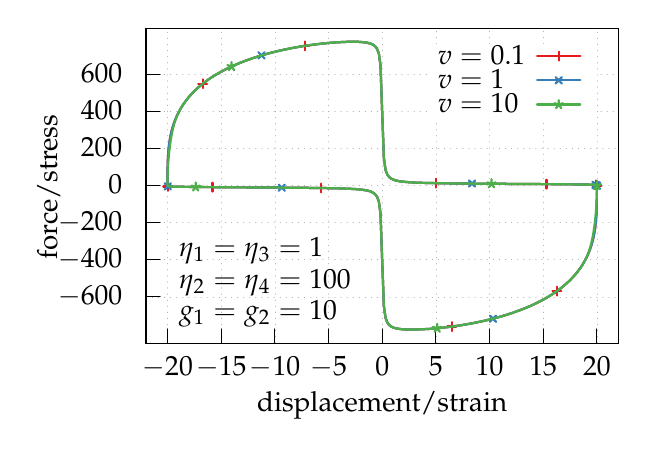
\begin{tikzpicture}[gnuplot]
%% generated with GNUPLOT 5.4p2 (Lua 5.4; terminal rev. Jun 2020, script rev. 114)
%% 11/05/21 19:23:17
\path (0.000,0.000) rectangle (6.000,4.000);
\gpcolor{color=gp lt color axes}
\gpsetlinetype{gp lt axes}
\gpsetdashtype{gp dt axes}
\gpsetlinewidth{0.50}
\draw[gp path] (0.000,0.588)--(5.999,0.588);
\gpcolor{color=gp lt color border}
\gpsetlinetype{gp lt border}
\gpsetdashtype{gp dt solid}
\gpsetlinewidth{1.00}
\draw[gp path] (0.000,0.588)--(0.180,0.588);
\node[gp node right] at (-0.184,0.588) {$-600$};
\gpcolor{color=gp lt color axes}
\gpsetlinetype{gp lt axes}
\gpsetdashtype{gp dt axes}
\gpsetlinewidth{0.50}
\draw[gp path] (0.000,1.059)--(5.999,1.059);
\gpcolor{color=gp lt color border}
\gpsetlinetype{gp lt border}
\gpsetdashtype{gp dt solid}
\gpsetlinewidth{1.00}
\draw[gp path] (0.000,1.059)--(0.180,1.059);
\node[gp node right] at (-0.184,1.059) {$-400$};
\gpcolor{color=gp lt color axes}
\gpsetlinetype{gp lt axes}
\gpsetdashtype{gp dt axes}
\gpsetlinewidth{0.50}
\draw[gp path] (0.000,1.529)--(5.999,1.529);
\gpcolor{color=gp lt color border}
\gpsetlinetype{gp lt border}
\gpsetdashtype{gp dt solid}
\gpsetlinewidth{1.00}
\draw[gp path] (0.000,1.529)--(0.180,1.529);
\node[gp node right] at (-0.184,1.529) {$-200$};
\gpcolor{color=gp lt color axes}
\gpsetlinetype{gp lt axes}
\gpsetdashtype{gp dt axes}
\gpsetlinewidth{0.50}
\draw[gp path] (0.000,2.000)--(5.999,2.000);
\gpcolor{color=gp lt color border}
\gpsetlinetype{gp lt border}
\gpsetdashtype{gp dt solid}
\gpsetlinewidth{1.00}
\draw[gp path] (0.000,2.000)--(0.180,2.000);
\node[gp node right] at (-0.184,2.000) {$0$};
\gpcolor{color=gp lt color axes}
\gpsetlinetype{gp lt axes}
\gpsetdashtype{gp dt axes}
\gpsetlinewidth{0.50}
\draw[gp path] (0.000,2.470)--(5.999,2.470);
\gpcolor{color=gp lt color border}
\gpsetlinetype{gp lt border}
\gpsetdashtype{gp dt solid}
\gpsetlinewidth{1.00}
\draw[gp path] (0.000,2.470)--(0.180,2.470);
\node[gp node right] at (-0.184,2.470) {$200$};
\gpcolor{color=gp lt color axes}
\gpsetlinetype{gp lt axes}
\gpsetdashtype{gp dt axes}
\gpsetlinewidth{0.50}
\draw[gp path] (0.000,2.940)--(3.587,2.940);
\draw[gp path] (5.699,2.940)--(5.999,2.940);
\gpcolor{color=gp lt color border}
\gpsetlinetype{gp lt border}
\gpsetdashtype{gp dt solid}
\gpsetlinewidth{1.00}
\draw[gp path] (0.000,2.940)--(0.180,2.940);
\node[gp node right] at (-0.184,2.940) {$400$};
\gpcolor{color=gp lt color axes}
\gpsetlinetype{gp lt axes}
\gpsetdashtype{gp dt axes}
\gpsetlinewidth{0.50}
\draw[gp path] (0.000,3.411)--(3.587,3.411);
\draw[gp path] (5.699,3.411)--(5.999,3.411);
\gpcolor{color=gp lt color border}
\gpsetlinetype{gp lt border}
\gpsetdashtype{gp dt solid}
\gpsetlinewidth{1.00}
\draw[gp path] (0.000,3.411)--(0.180,3.411);
\node[gp node right] at (-0.184,3.411) {$600$};
\gpcolor{color=gp lt color axes}
\gpsetlinetype{gp lt axes}
\gpsetdashtype{gp dt axes}
\gpsetlinewidth{0.50}
\draw[gp path] (0.273,0.000)--(0.273,3.999);
\gpcolor{color=gp lt color border}
\gpsetlinetype{gp lt border}
\gpsetdashtype{gp dt solid}
\gpsetlinewidth{1.00}
\draw[gp path] (0.273,0.000)--(0.273,0.180);
\node[gp node center] at (0.273,-0.308) {$-20$};
\gpcolor{color=gp lt color axes}
\gpsetlinetype{gp lt axes}
\gpsetdashtype{gp dt axes}
\gpsetlinewidth{0.50}
\draw[gp path] (0.954,0.000)--(0.954,3.999);
\gpcolor{color=gp lt color border}
\gpsetlinetype{gp lt border}
\gpsetdashtype{gp dt solid}
\gpsetlinewidth{1.00}
\draw[gp path] (0.954,0.000)--(0.954,0.180);
\node[gp node center] at (0.954,-0.308) {$-15$};
\gpcolor{color=gp lt color axes}
\gpsetlinetype{gp lt axes}
\gpsetdashtype{gp dt axes}
\gpsetlinewidth{0.50}
\draw[gp path] (1.636,0.000)--(1.636,3.999);
\gpcolor{color=gp lt color border}
\gpsetlinetype{gp lt border}
\gpsetdashtype{gp dt solid}
\gpsetlinewidth{1.00}
\draw[gp path] (1.636,0.000)--(1.636,0.180);
\node[gp node center] at (1.636,-0.308) {$-10$};
\gpcolor{color=gp lt color axes}
\gpsetlinetype{gp lt axes}
\gpsetdashtype{gp dt axes}
\gpsetlinewidth{0.50}
\draw[gp path] (2.318,0.000)--(2.318,3.999);
\gpcolor{color=gp lt color border}
\gpsetlinetype{gp lt border}
\gpsetdashtype{gp dt solid}
\gpsetlinewidth{1.00}
\draw[gp path] (2.318,0.000)--(2.318,0.180);
\node[gp node center] at (2.318,-0.308) {$-5$};
\gpcolor{color=gp lt color axes}
\gpsetlinetype{gp lt axes}
\gpsetdashtype{gp dt axes}
\gpsetlinewidth{0.50}
\draw[gp path] (3.000,0.000)--(3.000,3.999);
\gpcolor{color=gp lt color border}
\gpsetlinetype{gp lt border}
\gpsetdashtype{gp dt solid}
\gpsetlinewidth{1.00}
\draw[gp path] (3.000,0.000)--(3.000,0.180);
\node[gp node center] at (3.000,-0.308) {$0$};
\gpcolor{color=gp lt color axes}
\gpsetlinetype{gp lt axes}
\gpsetdashtype{gp dt axes}
\gpsetlinewidth{0.50}
\draw[gp path] (3.681,0.000)--(3.681,2.875);
\draw[gp path] (3.681,3.799)--(3.681,3.999);
\gpcolor{color=gp lt color border}
\gpsetlinetype{gp lt border}
\gpsetdashtype{gp dt solid}
\gpsetlinewidth{1.00}
\draw[gp path] (3.681,0.000)--(3.681,0.180);
\node[gp node center] at (3.681,-0.308) {$5$};
\gpcolor{color=gp lt color axes}
\gpsetlinetype{gp lt axes}
\gpsetdashtype{gp dt axes}
\gpsetlinewidth{0.50}
\draw[gp path] (4.363,0.000)--(4.363,2.875);
\draw[gp path] (4.363,3.799)--(4.363,3.999);
\gpcolor{color=gp lt color border}
\gpsetlinetype{gp lt border}
\gpsetdashtype{gp dt solid}
\gpsetlinewidth{1.00}
\draw[gp path] (4.363,0.000)--(4.363,0.180);
\node[gp node center] at (4.363,-0.308) {$10$};
\gpcolor{color=gp lt color axes}
\gpsetlinetype{gp lt axes}
\gpsetdashtype{gp dt axes}
\gpsetlinewidth{0.50}
\draw[gp path] (5.045,0.000)--(5.045,2.875);
\draw[gp path] (5.045,3.799)--(5.045,3.999);
\gpcolor{color=gp lt color border}
\gpsetlinetype{gp lt border}
\gpsetdashtype{gp dt solid}
\gpsetlinewidth{1.00}
\draw[gp path] (5.045,0.000)--(5.045,0.180);
\node[gp node center] at (5.045,-0.308) {$15$};
\gpcolor{color=gp lt color axes}
\gpsetlinetype{gp lt axes}
\gpsetdashtype{gp dt axes}
\gpsetlinewidth{0.50}
\draw[gp path] (5.726,0.000)--(5.726,3.999);
\gpcolor{color=gp lt color border}
\gpsetlinetype{gp lt border}
\gpsetdashtype{gp dt solid}
\gpsetlinewidth{1.00}
\draw[gp path] (5.726,0.000)--(5.726,0.180);
\node[gp node center] at (5.726,-0.308) {$20$};
\draw[gp path] (0.000,3.999)--(0.000,0.000)--(5.999,0.000)--(5.999,3.999)--cycle;
\node[gp node left] at (0.300,1.200) {$\eta_1=\eta_3=1$};
\node[gp node left] at (0.300,0.800) {$\eta_2=\eta_4=100$};
\node[gp node left] at (0.300,0.400) {$g_1=g_2=10$};
\node[gp node center,rotate=-270] at (-1.212,1.999) {force/stress};
\node[gp node center] at (2.999,-0.769) {displacement/strain};
\gpcolor{rgb color={0.894,0.102,0.110}}
\gpsetlinewidth{2.00}
\draw[gp path] (5.726,2.000)--(5.726,1.910)--(5.726,1.855)--(5.726,1.812)--(5.725,1.774)%
  --(5.724,1.740)--(5.723,1.709)--(5.722,1.680)--(5.721,1.652)--(5.720,1.626)--(5.718,1.601)%
  --(5.716,1.577)--(5.714,1.554)--(5.712,1.532)--(5.710,1.510)--(5.707,1.490)--(5.705,1.469)%
  --(5.702,1.449)--(5.699,1.430)--(5.696,1.411)--(5.693,1.393)--(5.689,1.375)--(5.686,1.357)%
  --(5.682,1.340)--(5.678,1.323)--(5.674,1.306)--(5.670,1.290)--(5.665,1.273)--(5.661,1.258)%
  --(5.656,1.242)--(5.651,1.227)--(5.646,1.211)--(5.641,1.196)--(5.635,1.182)--(5.630,1.167)%
  --(5.624,1.153)--(5.618,1.139)--(5.612,1.125)--(5.606,1.111)--(5.599,1.097)--(5.593,1.084)%
  --(5.586,1.071)--(5.579,1.058)--(5.572,1.045)--(5.565,1.032)--(5.558,1.019)--(5.550,1.007)%
  --(5.543,0.994)--(5.535,0.982)--(5.527,0.970)--(5.519,0.958)--(5.510,0.946)--(5.502,0.935)%
  --(5.493,0.923)--(5.485,0.912)--(5.476,0.900)--(5.467,0.889)--(5.458,0.878)--(5.448,0.867)%
  --(5.439,0.856)--(5.429,0.845)--(5.419,0.835)--(5.409,0.824)--(5.399,0.814)--(5.389,0.803)%
  --(5.379,0.793)--(5.368,0.783)--(5.357,0.773)--(5.347,0.763)--(5.336,0.753)--(5.324,0.743)%
  --(5.313,0.734)--(5.302,0.724)--(5.290,0.715)--(5.279,0.705)--(5.267,0.696)--(5.255,0.687)%
  --(5.243,0.678)--(5.230,0.669)--(5.218,0.660)--(5.206,0.651)--(5.193,0.643)--(5.180,0.634)%
  --(5.167,0.625)--(5.154,0.617)--(5.141,0.609)--(5.128,0.600)--(5.114,0.592)--(5.101,0.584)%
  --(5.087,0.576)--(5.073,0.568)--(5.059,0.560)--(5.045,0.553)--(5.031,0.545)--(5.016,0.537)%
  --(5.002,0.530)--(4.987,0.522)--(4.973,0.515)--(4.958,0.508)--(4.943,0.500)--(4.928,0.493)%
  --(4.912,0.486)--(4.897,0.479)--(4.882,0.472)--(4.866,0.466)--(4.850,0.459)--(4.835,0.452)%
  --(4.819,0.446)--(4.803,0.439)--(4.787,0.433)--(4.770,0.426)--(4.754,0.420)--(4.738,0.414)%
  --(4.721,0.408)--(4.704,0.402)--(4.688,0.396)--(4.671,0.390)--(4.654,0.384)--(4.637,0.378)%
  --(4.620,0.373)--(4.602,0.367)--(4.585,0.361)--(4.567,0.356)--(4.550,0.351)--(4.532,0.345)%
  --(4.514,0.340)--(4.497,0.335)--(4.479,0.330)--(4.461,0.325)--(4.442,0.320)--(4.424,0.315)%
  --(4.406,0.310)--(4.388,0.306)--(4.369,0.301)--(4.351,0.297)--(4.332,0.292)--(4.313,0.288)%
  --(4.294,0.283)--(4.275,0.279)--(4.256,0.275)--(4.237,0.271)--(4.218,0.267)--(4.199,0.263)%
  --(4.180,0.259)--(4.161,0.255)--(4.141,0.251)--(4.122,0.248)--(4.102,0.244)--(4.082,0.241)%
  --(4.063,0.237)--(4.043,0.234)--(4.023,0.231)--(4.003,0.227)--(3.983,0.224)--(3.963,0.221)%
  --(3.943,0.218)--(3.923,0.215)--(3.903,0.213)--(3.883,0.210)--(3.862,0.207)--(3.842,0.205)%
  --(3.822,0.202)--(3.801,0.200)--(3.781,0.197)--(3.760,0.195)--(3.740,0.193)--(3.719,0.191)%
  --(3.698,0.189)--(3.678,0.187)--(3.657,0.185)--(3.636,0.184)--(3.615,0.182)--(3.594,0.180)%
  --(3.573,0.179)--(3.552,0.178)--(3.531,0.177)--(3.510,0.175)--(3.489,0.175)--(3.468,0.174)%
  --(3.447,0.173)--(3.426,0.173)--(3.405,0.172)--(3.384,0.172)--(3.362,0.172)--(3.341,0.172)%
  --(3.320,0.173)--(3.299,0.173)--(3.277,0.175)--(3.256,0.176)--(3.235,0.178)--(3.213,0.181)%
  --(3.192,0.184)--(3.171,0.189)--(3.149,0.195)--(3.128,0.203)--(3.107,0.215)--(3.085,0.233)%
  --(3.064,0.263)--(3.042,0.321)--(3.021,0.472)--(2.999,1.060)--(2.978,1.647)--(2.957,1.799)%
  --(2.935,1.857)--(2.914,1.887)--(2.892,1.905)--(2.871,1.917)--(2.850,1.926)--(2.828,1.933)%
  --(2.807,1.938)--(2.786,1.942)--(2.764,1.945)--(2.743,1.948)--(2.722,1.950)--(2.700,1.953)%
  --(2.679,1.954)--(2.658,1.956)--(2.637,1.957)--(2.615,1.958)--(2.594,1.960)--(2.573,1.961)%
  --(2.552,1.961)--(2.531,1.962)--(2.510,1.963)--(2.489,1.964)--(2.468,1.964)--(2.447,1.965)%
  --(2.426,1.966)--(2.405,1.966)--(2.384,1.967)--(2.363,1.967)--(2.342,1.967)--(2.321,1.968)%
  --(2.301,1.968)--(2.280,1.969)--(2.259,1.969)--(2.239,1.969)--(2.218,1.970)--(2.198,1.970)%
  --(2.177,1.970)--(2.157,1.970)--(2.137,1.971)--(2.116,1.971)--(2.096,1.971)--(2.076,1.971)%
  --(2.056,1.972)--(2.036,1.972)--(2.016,1.972)--(1.996,1.972)--(1.976,1.972)--(1.956,1.973)%
  --(1.936,1.973)--(1.917,1.973)--(1.897,1.973)--(1.877,1.973)--(1.858,1.973)--(1.838,1.974)%
  --(1.819,1.974)--(1.800,1.974)--(1.781,1.974)--(1.762,1.974)--(1.743,1.974)--(1.724,1.974)%
  --(1.705,1.975)--(1.686,1.975)--(1.667,1.975)--(1.648,1.975)--(1.630,1.975)--(1.611,1.975)%
  --(1.593,1.975)--(1.575,1.976)--(1.557,1.976)--(1.538,1.976)--(1.520,1.976)--(1.502,1.976)%
  --(1.485,1.976)--(1.467,1.976)--(1.449,1.976)--(1.432,1.976)--(1.414,1.977)--(1.397,1.977)%
  --(1.379,1.977)--(1.362,1.977)--(1.345,1.977)--(1.328,1.977)--(1.311,1.977)--(1.295,1.977)%
  --(1.278,1.977)--(1.261,1.978)--(1.245,1.978)--(1.229,1.978)--(1.212,1.978)--(1.196,1.978)%
  --(1.180,1.978)--(1.164,1.978)--(1.149,1.978)--(1.133,1.978)--(1.117,1.979)--(1.102,1.979)%
  --(1.087,1.979)--(1.071,1.979)--(1.056,1.979)--(1.041,1.979)--(1.026,1.979)--(1.012,1.979)%
  --(0.997,1.979)--(0.983,1.980)--(0.968,1.980)--(0.954,1.980)--(0.940,1.980)--(0.926,1.980)%
  --(0.912,1.980)--(0.898,1.980)--(0.885,1.980)--(0.871,1.980)--(0.858,1.980)--(0.845,1.981)%
  --(0.832,1.981)--(0.819,1.981)--(0.806,1.981)--(0.793,1.981)--(0.781,1.981)--(0.769,1.981)%
  --(0.756,1.981)--(0.744,1.981)--(0.732,1.982)--(0.720,1.982)--(0.709,1.982)--(0.697,1.982)%
  --(0.686,1.982)--(0.675,1.982)--(0.663,1.982)--(0.652,1.982)--(0.642,1.982)--(0.631,1.983)%
  --(0.620,1.983)--(0.610,1.983)--(0.600,1.983)--(0.590,1.983)--(0.580,1.983)--(0.570,1.983)%
  --(0.560,1.983)--(0.551,1.984)--(0.541,1.984)--(0.532,1.984)--(0.523,1.984)--(0.514,1.984)%
  --(0.506,1.984)--(0.497,1.984)--(0.489,1.984)--(0.480,1.985)--(0.472,1.985)--(0.464,1.985)%
  --(0.456,1.985)--(0.449,1.985)--(0.441,1.985)--(0.434,1.985)--(0.427,1.985)--(0.420,1.986)%
  --(0.413,1.986)--(0.406,1.986)--(0.400,1.986)--(0.393,1.986)--(0.387,1.986)--(0.381,1.986)%
  --(0.375,1.986)--(0.369,1.987)--(0.364,1.987)--(0.358,1.987)--(0.353,1.987)--(0.348,1.987)%
  --(0.343,1.987)--(0.338,1.987)--(0.334,1.988)--(0.329,1.988)--(0.325,1.988)--(0.321,1.988)%
  --(0.317,1.988)--(0.313,1.988)--(0.310,1.988)--(0.306,1.989)--(0.303,1.989)--(0.300,1.989)%
  --(0.297,1.989)--(0.294,1.989)--(0.292,1.989)--(0.289,1.989)--(0.287,1.989)--(0.285,1.989)%
  --(0.283,1.990)--(0.281,1.990)--(0.279,1.990)--(0.278,1.990)--(0.277,1.990)--(0.276,1.990)%
  --(0.275,1.990)--(0.274,1.989)--(0.273,1.989)--(0.273,1.988)--(0.273,1.986)--(0.273,2.000)%
  --(0.273,2.089)--(0.273,2.144)--(0.273,2.187)--(0.274,2.225)--(0.275,2.259)--(0.276,2.290)%
  --(0.277,2.319)--(0.278,2.347)--(0.279,2.373)--(0.281,2.398)--(0.283,2.422)--(0.285,2.445)%
  --(0.287,2.467)--(0.289,2.489)--(0.292,2.509)--(0.294,2.530)--(0.297,2.550)--(0.300,2.569)%
  --(0.303,2.588)--(0.306,2.606)--(0.310,2.624)--(0.313,2.642)--(0.317,2.659)--(0.321,2.676)%
  --(0.325,2.693)--(0.329,2.709)--(0.334,2.726)--(0.338,2.741)--(0.343,2.757)--(0.348,2.772)%
  --(0.353,2.788)--(0.358,2.803)--(0.364,2.817)--(0.369,2.832)--(0.375,2.846)--(0.381,2.860)%
  --(0.387,2.874)--(0.393,2.888)--(0.400,2.902)--(0.406,2.915)--(0.413,2.928)--(0.420,2.941)%
  --(0.427,2.954)--(0.434,2.967)--(0.441,2.980)--(0.449,2.992)--(0.456,3.005)--(0.464,3.017)%
  --(0.472,3.029)--(0.480,3.041)--(0.489,3.053)--(0.497,3.064)--(0.506,3.076)--(0.514,3.087)%
  --(0.523,3.099)--(0.532,3.110)--(0.541,3.121)--(0.551,3.132)--(0.560,3.143)--(0.570,3.154)%
  --(0.580,3.164)--(0.590,3.175)--(0.600,3.185)--(0.610,3.196)--(0.620,3.206)--(0.631,3.216)%
  --(0.642,3.226)--(0.652,3.236)--(0.663,3.246)--(0.675,3.256)--(0.686,3.265)--(0.697,3.275)%
  --(0.709,3.284)--(0.720,3.294)--(0.732,3.303)--(0.744,3.312)--(0.756,3.321)--(0.769,3.330)%
  --(0.781,3.339)--(0.793,3.348)--(0.806,3.356)--(0.819,3.365)--(0.832,3.374)--(0.845,3.382)%
  --(0.858,3.390)--(0.871,3.399)--(0.885,3.407)--(0.898,3.415)--(0.912,3.423)--(0.926,3.431)%
  --(0.940,3.439)--(0.954,3.446)--(0.968,3.454)--(0.983,3.462)--(0.997,3.469)--(1.012,3.477)%
  --(1.026,3.484)--(1.041,3.491)--(1.056,3.499)--(1.071,3.506)--(1.087,3.513)--(1.102,3.520)%
  --(1.117,3.527)--(1.133,3.533)--(1.149,3.540)--(1.164,3.547)--(1.180,3.553)--(1.196,3.560)%
  --(1.212,3.566)--(1.229,3.573)--(1.245,3.579)--(1.261,3.585)--(1.278,3.591)--(1.295,3.597)%
  --(1.311,3.603)--(1.328,3.609)--(1.345,3.615)--(1.362,3.621)--(1.379,3.626)--(1.397,3.632)%
  --(1.414,3.638)--(1.432,3.643)--(1.449,3.648)--(1.467,3.654)--(1.485,3.659)--(1.502,3.664)%
  --(1.520,3.669)--(1.538,3.674)--(1.557,3.679)--(1.575,3.684)--(1.593,3.689)--(1.611,3.693)%
  --(1.630,3.698)--(1.648,3.702)--(1.667,3.707)--(1.686,3.711)--(1.705,3.716)--(1.724,3.720)%
  --(1.743,3.724)--(1.762,3.728)--(1.781,3.732)--(1.800,3.736)--(1.819,3.740)--(1.838,3.744)%
  --(1.858,3.748)--(1.877,3.751)--(1.897,3.755)--(1.917,3.758)--(1.936,3.762)--(1.956,3.765)%
  --(1.976,3.768)--(1.996,3.772)--(2.016,3.775)--(2.036,3.778)--(2.056,3.781)--(2.076,3.784)%
  --(2.096,3.786)--(2.116,3.789)--(2.137,3.792)--(2.157,3.794)--(2.177,3.797)--(2.198,3.799)%
  --(2.218,3.802)--(2.239,3.804)--(2.259,3.806)--(2.280,3.808)--(2.301,3.810)--(2.321,3.812)%
  --(2.342,3.814)--(2.363,3.815)--(2.384,3.817)--(2.405,3.819)--(2.426,3.820)--(2.447,3.821)%
  --(2.468,3.822)--(2.489,3.824)--(2.510,3.824)--(2.531,3.825)--(2.552,3.826)--(2.573,3.826)%
  --(2.594,3.827)--(2.615,3.827)--(2.637,3.827)--(2.658,3.827)--(2.679,3.826)--(2.700,3.826)%
  --(2.722,3.824)--(2.743,3.823)--(2.764,3.821)--(2.786,3.818)--(2.807,3.815)--(2.828,3.810)%
  --(2.850,3.804)--(2.871,3.796)--(2.892,3.784)--(2.914,3.766)--(2.935,3.736)--(2.957,3.678)%
  --(2.978,3.527)--(2.999,2.939)--(3.021,2.352)--(3.042,2.200)--(3.064,2.142)--(3.085,2.112)%
  --(3.107,2.094)--(3.128,2.082)--(3.149,2.073)--(3.171,2.066)--(3.192,2.061)--(3.213,2.057)%
  --(3.235,2.054)--(3.256,2.051)--(3.277,2.049)--(3.299,2.046)--(3.320,2.045)--(3.341,2.043)%
  --(3.362,2.042)--(3.384,2.041)--(3.405,2.039)--(3.426,2.038)--(3.447,2.038)--(3.468,2.037)%
  --(3.489,2.036)--(3.510,2.035)--(3.531,2.035)--(3.552,2.034)--(3.573,2.033)--(3.594,2.033)%
  --(3.615,2.032)--(3.636,2.032)--(3.657,2.032)--(3.678,2.031)--(3.698,2.031)--(3.719,2.030)%
  --(3.740,2.030)--(3.760,2.030)--(3.781,2.029)--(3.801,2.029)--(3.822,2.029)--(3.842,2.029)%
  --(3.862,2.028)--(3.883,2.028)--(3.903,2.028)--(3.923,2.028)--(3.943,2.027)--(3.963,2.027)%
  --(3.983,2.027)--(4.003,2.027)--(4.023,2.027)--(4.043,2.026)--(4.063,2.026)--(4.082,2.026)%
  --(4.102,2.026)--(4.122,2.026)--(4.141,2.026)--(4.161,2.025)--(4.180,2.025)--(4.199,2.025)%
  --(4.218,2.025)--(4.237,2.025)--(4.256,2.025)--(4.275,2.025)--(4.294,2.024)--(4.313,2.024)%
  --(4.332,2.024)--(4.351,2.024)--(4.369,2.024)--(4.388,2.024)--(4.406,2.024)--(4.424,2.023)%
  --(4.442,2.023)--(4.461,2.023)--(4.479,2.023)--(4.497,2.023)--(4.514,2.023)--(4.532,2.023)%
  --(4.550,2.023)--(4.567,2.023)--(4.585,2.022)--(4.602,2.022)--(4.620,2.022)--(4.637,2.022)%
  --(4.654,2.022)--(4.671,2.022)--(4.688,2.022)--(4.704,2.022)--(4.721,2.022)--(4.738,2.021)%
  --(4.754,2.021)--(4.770,2.021)--(4.787,2.021)--(4.803,2.021)--(4.819,2.021)--(4.835,2.021)%
  --(4.850,2.021)--(4.866,2.021)--(4.882,2.020)--(4.897,2.020)--(4.912,2.020)--(4.928,2.020)%
  --(4.943,2.020)--(4.958,2.020)--(4.973,2.020)--(4.987,2.020)--(5.002,2.020)--(5.016,2.019)%
  --(5.031,2.019)--(5.045,2.019)--(5.059,2.019)--(5.073,2.019)--(5.087,2.019)--(5.101,2.019)%
  --(5.114,2.019)--(5.128,2.019)--(5.141,2.019)--(5.154,2.018)--(5.167,2.018)--(5.180,2.018)%
  --(5.193,2.018)--(5.206,2.018)--(5.218,2.018)--(5.230,2.018)--(5.243,2.018)--(5.255,2.018)%
  --(5.267,2.017)--(5.279,2.017)--(5.290,2.017)--(5.302,2.017)--(5.313,2.017)--(5.324,2.017)%
  --(5.336,2.017)--(5.347,2.017)--(5.357,2.017)--(5.368,2.016)--(5.379,2.016)--(5.389,2.016)%
  --(5.399,2.016)--(5.409,2.016)--(5.419,2.016)--(5.429,2.016)--(5.439,2.016)--(5.448,2.015)%
  --(5.458,2.015)--(5.467,2.015)--(5.476,2.015)--(5.485,2.015)--(5.493,2.015)--(5.502,2.015)%
  --(5.510,2.015)--(5.519,2.014)--(5.527,2.014)--(5.535,2.014)--(5.543,2.014)--(5.550,2.014)%
  --(5.558,2.014)--(5.565,2.014)--(5.572,2.014)--(5.579,2.013)--(5.586,2.013)--(5.593,2.013)%
  --(5.599,2.013)--(5.606,2.013)--(5.612,2.013)--(5.618,2.013)--(5.624,2.013)--(5.630,2.012)%
  --(5.635,2.012)--(5.641,2.012)--(5.646,2.012)--(5.651,2.012)--(5.656,2.012)--(5.661,2.012)%
  --(5.665,2.011)--(5.670,2.011)--(5.674,2.011)--(5.678,2.011)--(5.682,2.011)--(5.686,2.011)%
  --(5.689,2.011)--(5.693,2.010)--(5.696,2.010)--(5.699,2.010)--(5.702,2.010)--(5.705,2.010)%
  --(5.707,2.010)--(5.710,2.010)--(5.712,2.010)--(5.714,2.010)--(5.716,2.009)--(5.718,2.009)%
  --(5.720,2.009)--(5.721,2.009)--(5.722,2.009)--(5.723,2.009)--(5.724,2.009)--(5.725,2.010)%
  --(5.726,2.010)--(5.726,2.011)--(5.726,2.013)--cycle;
\gpsetpointsize{4.00}
\gp3point{gp mark 1}{}{(5.726,2.000)}
\gp3point{gp mark 1}{}{(5.218,0.660)}
\gp3point{gp mark 1}{}{(3.883,0.210)}
\gp3point{gp mark 1}{}{(2.218,1.970)}
\gp3point{gp mark 1}{}{(0.845,1.981)}
\gp3point{gp mark 1}{}{(0.275,1.990)}
\gp3point{gp mark 1}{}{(0.720,3.294)}
\gp3point{gp mark 1}{}{(2.016,3.775)}
\gp3point{gp mark 1}{}{(3.678,2.031)}
\gp3point{gp mark 1}{}{(5.087,2.019)}
\gp3point{gp mark 1}{}{(5.718,2.009)}
\gpcolor{rgb color={0.216,0.494,0.722}}
\draw[gp path] (5.726,2.000)--(5.726,1.939)--(5.726,1.874)--(5.726,1.818)--(5.725,1.774)%
  --(5.724,1.740)--(5.723,1.709)--(5.722,1.680)--(5.721,1.652)--(5.720,1.626)--(5.718,1.601)%
  --(5.716,1.577)--(5.714,1.554)--(5.712,1.532)--(5.710,1.510)--(5.707,1.490)--(5.705,1.469)%
  --(5.702,1.449)--(5.699,1.430)--(5.696,1.411)--(5.693,1.393)--(5.689,1.375)--(5.686,1.357)%
  --(5.682,1.340)--(5.678,1.323)--(5.674,1.306)--(5.670,1.290)--(5.665,1.273)--(5.661,1.258)%
  --(5.656,1.242)--(5.651,1.227)--(5.646,1.211)--(5.641,1.196)--(5.635,1.182)--(5.630,1.167)%
  --(5.624,1.153)--(5.618,1.139)--(5.612,1.125)--(5.606,1.111)--(5.599,1.097)--(5.593,1.084)%
  --(5.586,1.071)--(5.579,1.058)--(5.572,1.045)--(5.565,1.032)--(5.558,1.019)--(5.550,1.007)%
  --(5.543,0.994)--(5.535,0.982)--(5.527,0.970)--(5.519,0.958)--(5.510,0.946)--(5.502,0.935)%
  --(5.493,0.923)--(5.485,0.912)--(5.476,0.900)--(5.467,0.889)--(5.458,0.878)--(5.448,0.867)%
  --(5.439,0.856)--(5.429,0.845)--(5.419,0.835)--(5.409,0.824)--(5.399,0.814)--(5.389,0.803)%
  --(5.379,0.793)--(5.368,0.783)--(5.357,0.773)--(5.347,0.763)--(5.336,0.753)--(5.324,0.743)%
  --(5.313,0.734)--(5.302,0.724)--(5.290,0.715)--(5.279,0.705)--(5.267,0.696)--(5.255,0.687)%
  --(5.243,0.678)--(5.230,0.669)--(5.218,0.660)--(5.206,0.651)--(5.193,0.643)--(5.180,0.634)%
  --(5.167,0.625)--(5.154,0.617)--(5.141,0.609)--(5.128,0.600)--(5.114,0.592)--(5.101,0.584)%
  --(5.087,0.576)--(5.073,0.568)--(5.059,0.560)--(5.045,0.553)--(5.031,0.545)--(5.016,0.537)%
  --(5.002,0.530)--(4.987,0.522)--(4.973,0.515)--(4.958,0.508)--(4.943,0.500)--(4.928,0.493)%
  --(4.912,0.486)--(4.897,0.479)--(4.882,0.472)--(4.866,0.466)--(4.850,0.459)--(4.835,0.452)%
  --(4.819,0.446)--(4.803,0.439)--(4.787,0.433)--(4.770,0.426)--(4.754,0.420)--(4.738,0.414)%
  --(4.721,0.408)--(4.704,0.402)--(4.688,0.396)--(4.671,0.390)--(4.654,0.384)--(4.637,0.378)%
  --(4.620,0.373)--(4.602,0.367)--(4.585,0.361)--(4.567,0.356)--(4.550,0.351)--(4.532,0.345)%
  --(4.514,0.340)--(4.497,0.335)--(4.479,0.330)--(4.461,0.325)--(4.442,0.320)--(4.424,0.315)%
  --(4.406,0.310)--(4.388,0.306)--(4.369,0.301)--(4.351,0.297)--(4.332,0.292)--(4.313,0.288)%
  --(4.294,0.283)--(4.275,0.279)--(4.256,0.275)--(4.237,0.271)--(4.218,0.267)--(4.199,0.263)%
  --(4.180,0.259)--(4.161,0.255)--(4.141,0.251)--(4.122,0.248)--(4.102,0.244)--(4.082,0.241)%
  --(4.063,0.237)--(4.043,0.234)--(4.023,0.231)--(4.003,0.227)--(3.983,0.224)--(3.963,0.221)%
  --(3.943,0.218)--(3.923,0.215)--(3.903,0.213)--(3.883,0.210)--(3.862,0.207)--(3.842,0.205)%
  --(3.822,0.202)--(3.801,0.200)--(3.781,0.197)--(3.760,0.195)--(3.740,0.193)--(3.719,0.191)%
  --(3.698,0.189)--(3.678,0.187)--(3.657,0.185)--(3.636,0.184)--(3.615,0.182)--(3.594,0.180)%
  --(3.573,0.179)--(3.552,0.178)--(3.531,0.177)--(3.510,0.175)--(3.489,0.175)--(3.468,0.174)%
  --(3.447,0.173)--(3.426,0.173)--(3.405,0.172)--(3.384,0.172)--(3.362,0.172)--(3.341,0.172)%
  --(3.320,0.173)--(3.299,0.173)--(3.277,0.175)--(3.256,0.176)--(3.235,0.178)--(3.213,0.181)%
  --(3.192,0.184)--(3.171,0.189)--(3.149,0.195)--(3.128,0.203)--(3.107,0.215)--(3.085,0.233)%
  --(3.064,0.263)--(3.042,0.321)--(3.021,0.472)--(2.999,1.060)--(2.978,1.647)--(2.957,1.799)%
  --(2.935,1.857)--(2.914,1.887)--(2.892,1.905)--(2.871,1.917)--(2.850,1.926)--(2.828,1.933)%
  --(2.807,1.938)--(2.786,1.942)--(2.764,1.945)--(2.743,1.948)--(2.722,1.950)--(2.700,1.953)%
  --(2.679,1.954)--(2.658,1.956)--(2.637,1.957)--(2.615,1.958)--(2.594,1.960)--(2.573,1.961)%
  --(2.552,1.961)--(2.531,1.962)--(2.510,1.963)--(2.489,1.964)--(2.468,1.964)--(2.447,1.965)%
  --(2.426,1.966)--(2.405,1.966)--(2.384,1.967)--(2.363,1.967)--(2.342,1.967)--(2.321,1.968)%
  --(2.301,1.968)--(2.280,1.969)--(2.259,1.969)--(2.239,1.969)--(2.218,1.970)--(2.198,1.970)%
  --(2.177,1.970)--(2.157,1.970)--(2.137,1.971)--(2.116,1.971)--(2.096,1.971)--(2.076,1.971)%
  --(2.056,1.972)--(2.036,1.972)--(2.016,1.972)--(1.996,1.972)--(1.976,1.972)--(1.956,1.973)%
  --(1.936,1.973)--(1.917,1.973)--(1.897,1.973)--(1.877,1.973)--(1.858,1.973)--(1.838,1.974)%
  --(1.819,1.974)--(1.800,1.974)--(1.781,1.974)--(1.762,1.974)--(1.743,1.974)--(1.724,1.974)%
  --(1.705,1.975)--(1.686,1.975)--(1.667,1.975)--(1.648,1.975)--(1.630,1.975)--(1.611,1.975)%
  --(1.593,1.975)--(1.575,1.976)--(1.557,1.976)--(1.538,1.976)--(1.520,1.976)--(1.502,1.976)%
  --(1.485,1.976)--(1.467,1.976)--(1.449,1.976)--(1.432,1.976)--(1.414,1.977)--(1.397,1.977)%
  --(1.379,1.977)--(1.362,1.977)--(1.345,1.977)--(1.328,1.977)--(1.311,1.977)--(1.295,1.977)%
  --(1.278,1.977)--(1.261,1.978)--(1.245,1.978)--(1.229,1.978)--(1.212,1.978)--(1.196,1.978)%
  --(1.180,1.978)--(1.164,1.978)--(1.149,1.978)--(1.133,1.978)--(1.117,1.979)--(1.102,1.979)%
  --(1.087,1.979)--(1.071,1.979)--(1.056,1.979)--(1.041,1.979)--(1.026,1.979)--(1.012,1.979)%
  --(0.997,1.979)--(0.983,1.980)--(0.968,1.980)--(0.954,1.980)--(0.940,1.980)--(0.926,1.980)%
  --(0.912,1.980)--(0.898,1.980)--(0.885,1.980)--(0.871,1.980)--(0.858,1.980)--(0.845,1.981)%
  --(0.832,1.981)--(0.819,1.981)--(0.806,1.981)--(0.793,1.981)--(0.781,1.981)--(0.769,1.981)%
  --(0.756,1.981)--(0.744,1.981)--(0.732,1.982)--(0.720,1.982)--(0.709,1.982)--(0.697,1.982)%
  --(0.686,1.982)--(0.675,1.982)--(0.663,1.982)--(0.652,1.982)--(0.642,1.982)--(0.631,1.983)%
  --(0.620,1.983)--(0.610,1.983)--(0.600,1.983)--(0.590,1.983)--(0.580,1.983)--(0.570,1.983)%
  --(0.560,1.983)--(0.551,1.984)--(0.541,1.984)--(0.532,1.984)--(0.523,1.984)--(0.514,1.984)%
  --(0.506,1.984)--(0.497,1.984)--(0.489,1.984)--(0.480,1.985)--(0.472,1.985)--(0.464,1.985)%
  --(0.456,1.985)--(0.449,1.985)--(0.441,1.985)--(0.434,1.985)--(0.427,1.985)--(0.420,1.986)%
  --(0.413,1.986)--(0.406,1.986)--(0.400,1.986)--(0.393,1.986)--(0.387,1.986)--(0.381,1.986)%
  --(0.375,1.986)--(0.369,1.987)--(0.364,1.987)--(0.358,1.987)--(0.353,1.987)--(0.348,1.987)%
  --(0.343,1.987)--(0.338,1.987)--(0.334,1.988)--(0.329,1.988)--(0.325,1.988)--(0.321,1.988)%
  --(0.317,1.988)--(0.313,1.988)--(0.310,1.988)--(0.306,1.989)--(0.303,1.989)--(0.300,1.989)%
  --(0.297,1.989)--(0.294,1.989)--(0.292,1.989)--(0.289,1.989)--(0.287,1.989)--(0.285,1.989)%
  --(0.283,1.990)--(0.281,1.990)--(0.279,1.990)--(0.278,1.990)--(0.277,1.990)--(0.276,1.990)%
  --(0.275,1.990)--(0.274,1.989)--(0.273,1.989)--(0.273,1.990)--(0.273,2.000)--(0.273,2.060)%
  --(0.273,2.125)--(0.273,2.181)--(0.274,2.225)--(0.275,2.259)--(0.276,2.290)--(0.277,2.319)%
  --(0.278,2.347)--(0.279,2.373)--(0.281,2.398)--(0.283,2.422)--(0.285,2.445)--(0.287,2.467)%
  --(0.289,2.489)--(0.292,2.509)--(0.294,2.530)--(0.297,2.550)--(0.300,2.569)--(0.303,2.588)%
  --(0.306,2.606)--(0.310,2.624)--(0.313,2.642)--(0.317,2.659)--(0.321,2.676)--(0.325,2.693)%
  --(0.329,2.709)--(0.334,2.726)--(0.338,2.741)--(0.343,2.757)--(0.348,2.772)--(0.353,2.788)%
  --(0.358,2.803)--(0.364,2.817)--(0.369,2.832)--(0.375,2.846)--(0.381,2.860)--(0.387,2.874)%
  --(0.393,2.888)--(0.400,2.902)--(0.406,2.915)--(0.413,2.928)--(0.420,2.941)--(0.427,2.954)%
  --(0.434,2.967)--(0.441,2.980)--(0.449,2.992)--(0.456,3.005)--(0.464,3.017)--(0.472,3.029)%
  --(0.480,3.041)--(0.489,3.053)--(0.497,3.064)--(0.506,3.076)--(0.514,3.087)--(0.523,3.099)%
  --(0.532,3.110)--(0.541,3.121)--(0.551,3.132)--(0.560,3.143)--(0.570,3.154)--(0.580,3.164)%
  --(0.590,3.175)--(0.600,3.185)--(0.610,3.196)--(0.620,3.206)--(0.631,3.216)--(0.642,3.226)%
  --(0.652,3.236)--(0.663,3.246)--(0.675,3.256)--(0.686,3.265)--(0.697,3.275)--(0.709,3.284)%
  --(0.720,3.294)--(0.732,3.303)--(0.744,3.312)--(0.756,3.321)--(0.769,3.330)--(0.781,3.339)%
  --(0.793,3.348)--(0.806,3.356)--(0.819,3.365)--(0.832,3.374)--(0.845,3.382)--(0.858,3.390)%
  --(0.871,3.399)--(0.885,3.407)--(0.898,3.415)--(0.912,3.423)--(0.926,3.431)--(0.940,3.439)%
  --(0.954,3.446)--(0.968,3.454)--(0.983,3.462)--(0.997,3.469)--(1.012,3.477)--(1.026,3.484)%
  --(1.041,3.491)--(1.056,3.499)--(1.071,3.506)--(1.087,3.513)--(1.102,3.520)--(1.117,3.527)%
  --(1.133,3.533)--(1.149,3.540)--(1.164,3.547)--(1.180,3.553)--(1.196,3.560)--(1.212,3.566)%
  --(1.229,3.573)--(1.245,3.579)--(1.261,3.585)--(1.278,3.591)--(1.295,3.597)--(1.311,3.603)%
  --(1.328,3.609)--(1.345,3.615)--(1.362,3.621)--(1.379,3.626)--(1.397,3.632)--(1.414,3.638)%
  --(1.432,3.643)--(1.449,3.648)--(1.467,3.654)--(1.485,3.659)--(1.502,3.664)--(1.520,3.669)%
  --(1.538,3.674)--(1.557,3.679)--(1.575,3.684)--(1.593,3.689)--(1.611,3.693)--(1.630,3.698)%
  --(1.648,3.702)--(1.667,3.707)--(1.686,3.711)--(1.705,3.716)--(1.724,3.720)--(1.743,3.724)%
  --(1.762,3.728)--(1.781,3.732)--(1.800,3.736)--(1.819,3.740)--(1.838,3.744)--(1.858,3.748)%
  --(1.877,3.751)--(1.897,3.755)--(1.917,3.758)--(1.936,3.762)--(1.956,3.765)--(1.976,3.768)%
  --(1.996,3.772)--(2.016,3.775)--(2.036,3.778)--(2.056,3.781)--(2.076,3.784)--(2.096,3.786)%
  --(2.116,3.789)--(2.137,3.792)--(2.157,3.794)--(2.177,3.797)--(2.198,3.799)--(2.218,3.802)%
  --(2.239,3.804)--(2.259,3.806)--(2.280,3.808)--(2.301,3.810)--(2.321,3.812)--(2.342,3.814)%
  --(2.363,3.815)--(2.384,3.817)--(2.405,3.819)--(2.426,3.820)--(2.447,3.821)--(2.468,3.822)%
  --(2.489,3.824)--(2.510,3.824)--(2.531,3.825)--(2.552,3.826)--(2.573,3.826)--(2.594,3.827)%
  --(2.615,3.827)--(2.637,3.827)--(2.658,3.827)--(2.679,3.826)--(2.700,3.826)--(2.722,3.824)%
  --(2.743,3.823)--(2.764,3.821)--(2.786,3.818)--(2.807,3.815)--(2.828,3.810)--(2.850,3.804)%
  --(2.871,3.796)--(2.892,3.784)--(2.914,3.766)--(2.935,3.736)--(2.957,3.678)--(2.978,3.527)%
  --(2.999,2.939)--(3.021,2.352)--(3.042,2.200)--(3.064,2.142)--(3.085,2.112)--(3.107,2.094)%
  --(3.128,2.082)--(3.149,2.073)--(3.171,2.066)--(3.192,2.061)--(3.213,2.057)--(3.235,2.054)%
  --(3.256,2.051)--(3.277,2.049)--(3.299,2.046)--(3.320,2.045)--(3.341,2.043)--(3.362,2.042)%
  --(3.384,2.041)--(3.405,2.039)--(3.426,2.038)--(3.447,2.038)--(3.468,2.037)--(3.489,2.036)%
  --(3.510,2.035)--(3.531,2.035)--(3.552,2.034)--(3.573,2.033)--(3.594,2.033)--(3.615,2.032)%
  --(3.636,2.032)--(3.657,2.032)--(3.678,2.031)--(3.698,2.031)--(3.719,2.030)--(3.740,2.030)%
  --(3.760,2.030)--(3.781,2.029)--(3.801,2.029)--(3.822,2.029)--(3.842,2.029)--(3.862,2.028)%
  --(3.883,2.028)--(3.903,2.028)--(3.923,2.028)--(3.943,2.027)--(3.963,2.027)--(3.983,2.027)%
  --(4.003,2.027)--(4.023,2.027)--(4.043,2.026)--(4.063,2.026)--(4.082,2.026)--(4.102,2.026)%
  --(4.122,2.026)--(4.141,2.026)--(4.161,2.025)--(4.180,2.025)--(4.199,2.025)--(4.218,2.025)%
  --(4.237,2.025)--(4.256,2.025)--(4.275,2.025)--(4.294,2.024)--(4.313,2.024)--(4.332,2.024)%
  --(4.351,2.024)--(4.369,2.024)--(4.388,2.024)--(4.406,2.024)--(4.424,2.023)--(4.442,2.023)%
  --(4.461,2.023)--(4.479,2.023)--(4.497,2.023)--(4.514,2.023)--(4.532,2.023)--(4.550,2.023)%
  --(4.567,2.023)--(4.585,2.022)--(4.602,2.022)--(4.620,2.022)--(4.637,2.022)--(4.654,2.022)%
  --(4.671,2.022)--(4.688,2.022)--(4.704,2.022)--(4.721,2.022)--(4.738,2.021)--(4.754,2.021)%
  --(4.770,2.021)--(4.787,2.021)--(4.803,2.021)--(4.819,2.021)--(4.835,2.021)--(4.850,2.021)%
  --(4.866,2.021)--(4.882,2.020)--(4.897,2.020)--(4.912,2.020)--(4.928,2.020)--(4.943,2.020)%
  --(4.958,2.020)--(4.973,2.020)--(4.987,2.020)--(5.002,2.020)--(5.016,2.019)--(5.031,2.019)%
  --(5.045,2.019)--(5.059,2.019)--(5.073,2.019)--(5.087,2.019)--(5.101,2.019)--(5.114,2.019)%
  --(5.128,2.019)--(5.141,2.019)--(5.154,2.018)--(5.167,2.018)--(5.180,2.018)--(5.193,2.018)%
  --(5.206,2.018)--(5.218,2.018)--(5.230,2.018)--(5.243,2.018)--(5.255,2.018)--(5.267,2.017)%
  --(5.279,2.017)--(5.290,2.017)--(5.302,2.017)--(5.313,2.017)--(5.324,2.017)--(5.336,2.017)%
  --(5.347,2.017)--(5.357,2.017)--(5.368,2.016)--(5.379,2.016)--(5.389,2.016)--(5.399,2.016)%
  --(5.409,2.016)--(5.419,2.016)--(5.429,2.016)--(5.439,2.016)--(5.448,2.015)--(5.458,2.015)%
  --(5.467,2.015)--(5.476,2.015)--(5.485,2.015)--(5.493,2.015)--(5.502,2.015)--(5.510,2.015)%
  --(5.519,2.014)--(5.527,2.014)--(5.535,2.014)--(5.543,2.014)--(5.550,2.014)--(5.558,2.014)%
  --(5.565,2.014)--(5.572,2.014)--(5.579,2.013)--(5.586,2.013)--(5.593,2.013)--(5.599,2.013)%
  --(5.606,2.013)--(5.612,2.013)--(5.618,2.013)--(5.624,2.013)--(5.630,2.012)--(5.635,2.012)%
  --(5.641,2.012)--(5.646,2.012)--(5.651,2.012)--(5.656,2.012)--(5.661,2.012)--(5.665,2.011)%
  --(5.670,2.011)--(5.674,2.011)--(5.678,2.011)--(5.682,2.011)--(5.686,2.011)--(5.689,2.011)%
  --(5.693,2.010)--(5.696,2.010)--(5.699,2.010)--(5.702,2.010)--(5.705,2.010)--(5.707,2.010)%
  --(5.710,2.010)--(5.712,2.010)--(5.714,2.010)--(5.716,2.009)--(5.718,2.009)--(5.720,2.009)%
  --(5.721,2.009)--(5.722,2.009)--(5.723,2.009)--(5.724,2.009)--(5.725,2.010)--(5.726,2.010)%
  --(5.726,2.009)--cycle;
\gp3point{gp mark 2}{}{(5.726,2.000)}
\gp3point{gp mark 2}{}{(4.406,0.310)}
\gp3point{gp mark 2}{}{(1.724,1.974)}
\gp3point{gp mark 2}{}{(0.277,1.990)}
\gp3point{gp mark 2}{}{(1.467,3.654)}
\gp3point{gp mark 2}{}{(4.141,2.026)}
\gp3point{gp mark 2}{}{(5.710,2.010)}
\gpcolor{rgb color={0.302,0.686,0.290}}
\draw[gp path] (5.726,2.000)--(5.726,1.975)--(5.726,1.948)--(5.726,1.920)--(5.725,1.892)%
  --(5.724,1.865)--(5.723,1.838)--(5.722,1.810)--(5.721,1.783)--(5.720,1.756)--(5.718,1.729)%
  --(5.716,1.703)--(5.714,1.676)--(5.712,1.650)--(5.710,1.624)--(5.707,1.598)--(5.705,1.573)%
  --(5.702,1.547)--(5.699,1.522)--(5.696,1.498)--(5.693,1.474)--(5.689,1.450)--(5.686,1.426)%
  --(5.682,1.403)--(5.678,1.380)--(5.674,1.358)--(5.670,1.336)--(5.665,1.315)--(5.661,1.294)%
  --(5.656,1.274)--(5.651,1.254)--(5.646,1.234)--(5.641,1.215)--(5.635,1.197)--(5.630,1.179)%
  --(5.624,1.162)--(5.618,1.145)--(5.612,1.129)--(5.606,1.114)--(5.599,1.099)--(5.593,1.084)%
  --(5.586,1.071)--(5.579,1.058)--(5.572,1.045)--(5.565,1.032)--(5.558,1.019)--(5.550,1.007)%
  --(5.543,0.994)--(5.535,0.982)--(5.527,0.970)--(5.519,0.958)--(5.510,0.946)--(5.502,0.935)%
  --(5.493,0.923)--(5.485,0.912)--(5.476,0.900)--(5.467,0.889)--(5.458,0.878)--(5.448,0.867)%
  --(5.439,0.856)--(5.429,0.845)--(5.419,0.835)--(5.409,0.824)--(5.399,0.814)--(5.389,0.803)%
  --(5.379,0.793)--(5.368,0.783)--(5.357,0.773)--(5.347,0.763)--(5.336,0.753)--(5.324,0.743)%
  --(5.313,0.734)--(5.302,0.724)--(5.290,0.715)--(5.279,0.705)--(5.267,0.696)--(5.255,0.687)%
  --(5.243,0.678)--(5.230,0.669)--(5.218,0.660)--(5.206,0.651)--(5.193,0.643)--(5.180,0.634)%
  --(5.167,0.625)--(5.154,0.617)--(5.141,0.609)--(5.128,0.600)--(5.114,0.592)--(5.101,0.584)%
  --(5.087,0.576)--(5.073,0.568)--(5.059,0.560)--(5.045,0.553)--(5.031,0.545)--(5.016,0.537)%
  --(5.002,0.530)--(4.987,0.522)--(4.973,0.515)--(4.958,0.508)--(4.943,0.500)--(4.928,0.493)%
  --(4.912,0.486)--(4.897,0.479)--(4.882,0.472)--(4.866,0.466)--(4.850,0.459)--(4.835,0.452)%
  --(4.819,0.446)--(4.803,0.439)--(4.787,0.433)--(4.770,0.426)--(4.754,0.420)--(4.738,0.414)%
  --(4.721,0.408)--(4.704,0.402)--(4.688,0.396)--(4.671,0.390)--(4.654,0.384)--(4.637,0.378)%
  --(4.620,0.373)--(4.602,0.367)--(4.585,0.361)--(4.567,0.356)--(4.550,0.351)--(4.532,0.345)%
  --(4.514,0.340)--(4.497,0.335)--(4.479,0.330)--(4.461,0.325)--(4.442,0.320)--(4.424,0.315)%
  --(4.406,0.310)--(4.388,0.306)--(4.369,0.301)--(4.351,0.297)--(4.332,0.292)--(4.313,0.288)%
  --(4.294,0.283)--(4.275,0.279)--(4.256,0.275)--(4.237,0.271)--(4.218,0.267)--(4.199,0.263)%
  --(4.180,0.259)--(4.161,0.255)--(4.141,0.251)--(4.122,0.248)--(4.102,0.244)--(4.082,0.241)%
  --(4.063,0.237)--(4.043,0.234)--(4.023,0.231)--(4.003,0.227)--(3.983,0.224)--(3.963,0.221)%
  --(3.943,0.218)--(3.923,0.215)--(3.903,0.213)--(3.883,0.210)--(3.862,0.207)--(3.842,0.205)%
  --(3.822,0.202)--(3.801,0.200)--(3.781,0.197)--(3.760,0.195)--(3.740,0.193)--(3.719,0.191)%
  --(3.698,0.189)--(3.678,0.187)--(3.657,0.185)--(3.636,0.184)--(3.615,0.182)--(3.594,0.180)%
  --(3.573,0.179)--(3.552,0.178)--(3.531,0.177)--(3.510,0.175)--(3.489,0.175)--(3.468,0.174)%
  --(3.447,0.173)--(3.426,0.173)--(3.405,0.172)--(3.384,0.172)--(3.362,0.172)--(3.341,0.172)%
  --(3.320,0.173)--(3.299,0.173)--(3.277,0.175)--(3.256,0.176)--(3.235,0.178)--(3.213,0.181)%
  --(3.192,0.184)--(3.171,0.189)--(3.149,0.195)--(3.128,0.203)--(3.107,0.215)--(3.085,0.233)%
  --(3.064,0.263)--(3.042,0.321)--(3.021,0.472)--(2.999,1.060)--(2.978,1.647)--(2.957,1.799)%
  --(2.935,1.857)--(2.914,1.887)--(2.892,1.905)--(2.871,1.917)--(2.850,1.926)--(2.828,1.933)%
  --(2.807,1.938)--(2.786,1.942)--(2.764,1.945)--(2.743,1.948)--(2.722,1.950)--(2.700,1.953)%
  --(2.679,1.954)--(2.658,1.956)--(2.637,1.957)--(2.615,1.958)--(2.594,1.960)--(2.573,1.961)%
  --(2.552,1.961)--(2.531,1.962)--(2.510,1.963)--(2.489,1.964)--(2.468,1.964)--(2.447,1.965)%
  --(2.426,1.966)--(2.405,1.966)--(2.384,1.967)--(2.363,1.967)--(2.342,1.967)--(2.321,1.968)%
  --(2.301,1.968)--(2.280,1.969)--(2.259,1.969)--(2.239,1.969)--(2.218,1.970)--(2.198,1.970)%
  --(2.177,1.970)--(2.157,1.970)--(2.137,1.971)--(2.116,1.971)--(2.096,1.971)--(2.076,1.971)%
  --(2.056,1.972)--(2.036,1.972)--(2.016,1.972)--(1.996,1.972)--(1.976,1.972)--(1.956,1.973)%
  --(1.936,1.973)--(1.917,1.973)--(1.897,1.973)--(1.877,1.973)--(1.858,1.973)--(1.838,1.974)%
  --(1.819,1.974)--(1.800,1.974)--(1.781,1.974)--(1.762,1.974)--(1.743,1.974)--(1.724,1.974)%
  --(1.705,1.975)--(1.686,1.975)--(1.667,1.975)--(1.648,1.975)--(1.630,1.975)--(1.611,1.975)%
  --(1.593,1.975)--(1.575,1.976)--(1.557,1.976)--(1.538,1.976)--(1.520,1.976)--(1.502,1.976)%
  --(1.485,1.976)--(1.467,1.976)--(1.449,1.976)--(1.432,1.976)--(1.414,1.977)--(1.397,1.977)%
  --(1.379,1.977)--(1.362,1.977)--(1.345,1.977)--(1.328,1.977)--(1.311,1.977)--(1.295,1.977)%
  --(1.278,1.977)--(1.261,1.978)--(1.245,1.978)--(1.229,1.978)--(1.212,1.978)--(1.196,1.978)%
  --(1.180,1.978)--(1.164,1.978)--(1.149,1.978)--(1.133,1.978)--(1.117,1.979)--(1.102,1.979)%
  --(1.087,1.979)--(1.071,1.979)--(1.056,1.979)--(1.041,1.979)--(1.026,1.979)--(1.012,1.979)%
  --(0.997,1.979)--(0.983,1.980)--(0.968,1.980)--(0.954,1.980)--(0.940,1.980)--(0.926,1.980)%
  --(0.912,1.980)--(0.898,1.980)--(0.885,1.980)--(0.871,1.980)--(0.858,1.980)--(0.845,1.981)%
  --(0.832,1.981)--(0.819,1.981)--(0.806,1.981)--(0.793,1.981)--(0.781,1.981)--(0.769,1.981)%
  --(0.756,1.981)--(0.744,1.981)--(0.732,1.982)--(0.720,1.982)--(0.709,1.982)--(0.697,1.982)%
  --(0.686,1.982)--(0.675,1.982)--(0.663,1.982)--(0.652,1.982)--(0.642,1.982)--(0.631,1.983)%
  --(0.620,1.983)--(0.610,1.983)--(0.600,1.983)--(0.590,1.983)--(0.580,1.983)--(0.570,1.983)%
  --(0.560,1.983)--(0.551,1.984)--(0.541,1.984)--(0.532,1.984)--(0.523,1.984)--(0.514,1.984)%
  --(0.506,1.984)--(0.497,1.984)--(0.489,1.984)--(0.480,1.985)--(0.472,1.985)--(0.464,1.985)%
  --(0.456,1.985)--(0.449,1.985)--(0.441,1.985)--(0.434,1.985)--(0.427,1.985)--(0.420,1.986)%
  --(0.413,1.986)--(0.406,1.986)--(0.400,1.986)--(0.393,1.986)--(0.387,1.986)--(0.381,1.986)%
  --(0.375,1.987)--(0.369,1.987)--(0.364,1.987)--(0.358,1.987)--(0.353,1.987)--(0.348,1.988)%
  --(0.343,1.988)--(0.338,1.988)--(0.334,1.988)--(0.329,1.988)--(0.325,1.989)--(0.321,1.989)%
  --(0.317,1.989)--(0.313,1.989)--(0.310,1.990)--(0.306,1.990)--(0.303,1.990)--(0.300,1.991)%
  --(0.297,1.991)--(0.294,1.991)--(0.292,1.991)--(0.289,1.992)--(0.287,1.992)--(0.285,1.992)%
  --(0.283,1.993)--(0.281,1.993)--(0.279,1.993)--(0.278,1.993)--(0.277,1.994)--(0.276,1.994)%
  --(0.275,1.994)--(0.274,1.995)--(0.273,1.995)--(0.273,1.996)--(0.273,2.000)--(0.273,2.024)%
  --(0.273,2.051)--(0.273,2.079)--(0.274,2.107)--(0.275,2.134)--(0.276,2.161)--(0.277,2.189)%
  --(0.278,2.216)--(0.279,2.243)--(0.281,2.270)--(0.283,2.296)--(0.285,2.323)--(0.287,2.349)%
  --(0.289,2.375)--(0.292,2.401)--(0.294,2.426)--(0.297,2.452)--(0.300,2.477)--(0.303,2.501)%
  --(0.306,2.525)--(0.310,2.549)--(0.313,2.573)--(0.317,2.596)--(0.321,2.619)--(0.325,2.641)%
  --(0.329,2.663)--(0.334,2.684)--(0.338,2.705)--(0.343,2.725)--(0.348,2.745)--(0.353,2.765)%
  --(0.358,2.784)--(0.364,2.802)--(0.369,2.820)--(0.375,2.837)--(0.381,2.854)--(0.387,2.870)%
  --(0.393,2.885)--(0.400,2.900)--(0.406,2.915)--(0.413,2.928)--(0.420,2.941)--(0.427,2.954)%
  --(0.434,2.967)--(0.441,2.980)--(0.449,2.992)--(0.456,3.005)--(0.464,3.017)--(0.472,3.029)%
  --(0.480,3.041)--(0.489,3.053)--(0.497,3.064)--(0.506,3.076)--(0.514,3.087)--(0.523,3.099)%
  --(0.532,3.110)--(0.541,3.121)--(0.551,3.132)--(0.560,3.143)--(0.570,3.154)--(0.580,3.164)%
  --(0.590,3.175)--(0.600,3.185)--(0.610,3.196)--(0.620,3.206)--(0.631,3.216)--(0.642,3.226)%
  --(0.652,3.236)--(0.663,3.246)--(0.675,3.256)--(0.686,3.265)--(0.697,3.275)--(0.709,3.284)%
  --(0.720,3.294)--(0.732,3.303)--(0.744,3.312)--(0.756,3.321)--(0.769,3.330)--(0.781,3.339)%
  --(0.793,3.348)--(0.806,3.356)--(0.819,3.365)--(0.832,3.374)--(0.845,3.382)--(0.858,3.390)%
  --(0.871,3.399)--(0.885,3.407)--(0.898,3.415)--(0.912,3.423)--(0.926,3.431)--(0.940,3.439)%
  --(0.954,3.446)--(0.968,3.454)--(0.983,3.462)--(0.997,3.469)--(1.012,3.477)--(1.026,3.484)%
  --(1.041,3.491)--(1.056,3.499)--(1.071,3.506)--(1.087,3.513)--(1.102,3.520)--(1.117,3.527)%
  --(1.133,3.533)--(1.149,3.540)--(1.164,3.547)--(1.180,3.553)--(1.196,3.560)--(1.212,3.566)%
  --(1.229,3.573)--(1.245,3.579)--(1.261,3.585)--(1.278,3.591)--(1.295,3.597)--(1.311,3.603)%
  --(1.328,3.609)--(1.345,3.615)--(1.362,3.621)--(1.379,3.626)--(1.397,3.632)--(1.414,3.638)%
  --(1.432,3.643)--(1.449,3.648)--(1.467,3.654)--(1.485,3.659)--(1.502,3.664)--(1.520,3.669)%
  --(1.538,3.674)--(1.557,3.679)--(1.575,3.684)--(1.593,3.689)--(1.611,3.693)--(1.630,3.698)%
  --(1.648,3.702)--(1.667,3.707)--(1.686,3.711)--(1.705,3.716)--(1.724,3.720)--(1.743,3.724)%
  --(1.762,3.728)--(1.781,3.732)--(1.800,3.736)--(1.819,3.740)--(1.838,3.744)--(1.858,3.748)%
  --(1.877,3.751)--(1.897,3.755)--(1.917,3.758)--(1.936,3.762)--(1.956,3.765)--(1.976,3.768)%
  --(1.996,3.772)--(2.016,3.775)--(2.036,3.778)--(2.056,3.781)--(2.076,3.784)--(2.096,3.786)%
  --(2.116,3.789)--(2.137,3.792)--(2.157,3.794)--(2.177,3.797)--(2.198,3.799)--(2.218,3.802)%
  --(2.239,3.804)--(2.259,3.806)--(2.280,3.808)--(2.301,3.810)--(2.321,3.812)--(2.342,3.814)%
  --(2.363,3.815)--(2.384,3.817)--(2.405,3.819)--(2.426,3.820)--(2.447,3.821)--(2.468,3.822)%
  --(2.489,3.824)--(2.510,3.824)--(2.531,3.825)--(2.552,3.826)--(2.573,3.826)--(2.594,3.827)%
  --(2.615,3.827)--(2.637,3.827)--(2.658,3.827)--(2.679,3.826)--(2.700,3.826)--(2.722,3.824)%
  --(2.743,3.823)--(2.764,3.821)--(2.786,3.818)--(2.807,3.815)--(2.828,3.810)--(2.850,3.804)%
  --(2.871,3.796)--(2.892,3.784)--(2.914,3.766)--(2.935,3.736)--(2.957,3.678)--(2.978,3.527)%
  --(2.999,2.939)--(3.021,2.352)--(3.042,2.200)--(3.064,2.142)--(3.085,2.112)--(3.107,2.094)%
  --(3.128,2.082)--(3.149,2.073)--(3.171,2.066)--(3.192,2.061)--(3.213,2.057)--(3.235,2.054)%
  --(3.256,2.051)--(3.277,2.049)--(3.299,2.046)--(3.320,2.045)--(3.341,2.043)--(3.362,2.042)%
  --(3.384,2.041)--(3.405,2.039)--(3.426,2.038)--(3.447,2.038)--(3.468,2.037)--(3.489,2.036)%
  --(3.510,2.035)--(3.531,2.035)--(3.552,2.034)--(3.573,2.033)--(3.594,2.033)--(3.615,2.032)%
  --(3.636,2.032)--(3.657,2.032)--(3.678,2.031)--(3.698,2.031)--(3.719,2.030)--(3.740,2.030)%
  --(3.760,2.030)--(3.781,2.029)--(3.801,2.029)--(3.822,2.029)--(3.842,2.029)--(3.862,2.028)%
  --(3.883,2.028)--(3.903,2.028)--(3.923,2.028)--(3.943,2.027)--(3.963,2.027)--(3.983,2.027)%
  --(4.003,2.027)--(4.023,2.027)--(4.043,2.026)--(4.063,2.026)--(4.082,2.026)--(4.102,2.026)%
  --(4.122,2.026)--(4.141,2.026)--(4.161,2.025)--(4.180,2.025)--(4.199,2.025)--(4.218,2.025)%
  --(4.237,2.025)--(4.256,2.025)--(4.275,2.025)--(4.294,2.024)--(4.313,2.024)--(4.332,2.024)%
  --(4.351,2.024)--(4.369,2.024)--(4.388,2.024)--(4.406,2.024)--(4.424,2.023)--(4.442,2.023)%
  --(4.461,2.023)--(4.479,2.023)--(4.497,2.023)--(4.514,2.023)--(4.532,2.023)--(4.550,2.023)%
  --(4.567,2.023)--(4.585,2.022)--(4.602,2.022)--(4.620,2.022)--(4.637,2.022)--(4.654,2.022)%
  --(4.671,2.022)--(4.688,2.022)--(4.704,2.022)--(4.721,2.022)--(4.738,2.021)--(4.754,2.021)%
  --(4.770,2.021)--(4.787,2.021)--(4.803,2.021)--(4.819,2.021)--(4.835,2.021)--(4.850,2.021)%
  --(4.866,2.021)--(4.882,2.020)--(4.897,2.020)--(4.912,2.020)--(4.928,2.020)--(4.943,2.020)%
  --(4.958,2.020)--(4.973,2.020)--(4.987,2.020)--(5.002,2.020)--(5.016,2.019)--(5.031,2.019)%
  --(5.045,2.019)--(5.059,2.019)--(5.073,2.019)--(5.087,2.019)--(5.101,2.019)--(5.114,2.019)%
  --(5.128,2.019)--(5.141,2.019)--(5.154,2.018)--(5.167,2.018)--(5.180,2.018)--(5.193,2.018)%
  --(5.206,2.018)--(5.218,2.018)--(5.230,2.018)--(5.243,2.018)--(5.255,2.018)--(5.267,2.017)%
  --(5.279,2.017)--(5.290,2.017)--(5.302,2.017)--(5.313,2.017)--(5.324,2.017)--(5.336,2.017)%
  --(5.347,2.017)--(5.357,2.017)--(5.368,2.016)--(5.379,2.016)--(5.389,2.016)--(5.399,2.016)%
  --(5.409,2.016)--(5.419,2.016)--(5.429,2.016)--(5.439,2.016)--(5.448,2.015)--(5.458,2.015)%
  --(5.467,2.015)--(5.476,2.015)--(5.485,2.015)--(5.493,2.015)--(5.502,2.015)--(5.510,2.015)%
  --(5.519,2.014)--(5.527,2.014)--(5.535,2.014)--(5.543,2.014)--(5.550,2.014)--(5.558,2.014)%
  --(5.565,2.014)--(5.572,2.014)--(5.579,2.013)--(5.586,2.013)--(5.593,2.013)--(5.599,2.013)%
  --(5.606,2.013)--(5.612,2.013)--(5.618,2.013)--(5.624,2.012)--(5.630,2.012)--(5.635,2.012)%
  --(5.641,2.012)--(5.646,2.012)--(5.651,2.011)--(5.656,2.011)--(5.661,2.011)--(5.665,2.011)%
  --(5.670,2.011)--(5.674,2.010)--(5.678,2.010)--(5.682,2.010)--(5.686,2.010)--(5.689,2.009)%
  --(5.693,2.009)--(5.696,2.009)--(5.699,2.008)--(5.702,2.008)--(5.705,2.008)--(5.707,2.008)%
  --(5.710,2.007)--(5.712,2.007)--(5.714,2.007)--(5.716,2.006)--(5.718,2.006)--(5.720,2.006)%
  --(5.721,2.006)--(5.722,2.005)--(5.723,2.005)--(5.724,2.005)--(5.725,2.004)--(5.726,2.004)%
  --(5.726,2.003)--cycle;
\gp3point{gp mark 3}{}{(5.726,2.000)}
\gp3point{gp mark 3}{}{(3.698,0.189)}
\gp3point{gp mark 3}{}{(0.631,1.983)}
\gp3point{gp mark 3}{}{(1.087,3.513)}
\gp3point{gp mark 3}{}{(4.388,2.024)}
\gpfill{color=gpbgfillcolor} (3.587,2.875)--(5.699,2.875)--(5.699,3.799)--(3.587,3.799)--cycle;
\gpcolor{color=gp lt color border}
\node[gp node left] at (3.587,3.645) {$v=0.1$};
\gpcolor{rgb color={0.894,0.102,0.110}}
\draw[gp path] (4.967,3.645)--(5.515,3.645);
\gp3point{gp mark 1}{}{(5.241,3.645)}
\gpcolor{color=gp lt color border}
\node[gp node left] at (3.587,3.337) {$v=1$};
\gpcolor{rgb color={0.216,0.494,0.722}}
\draw[gp path] (4.967,3.337)--(5.515,3.337);
\gp3point{gp mark 2}{}{(5.241,3.337)}
\gpcolor{color=gp lt color border}
\node[gp node left] at (3.587,3.029) {$v=10$};
\gpcolor{rgb color={0.302,0.686,0.290}}
\draw[gp path] (4.967,3.029)--(5.515,3.029);
\gp3point{gp mark 3}{}{(5.241,3.029)}
\gpcolor{color=gp lt color border}
\gpsetlinewidth{1.00}
\draw[gp path] (0.000,3.999)--(0.000,0.000)--(5.999,0.000)--(5.999,3.999)--cycle;
%% coordinates of the plot area
\gpdefrectangularnode{gp plot 1}{\pgfpoint{0.000cm}{0.000cm}}{\pgfpoint{5.999cm}{3.999cm}}
\end{tikzpicture}
%% gnuplot variables

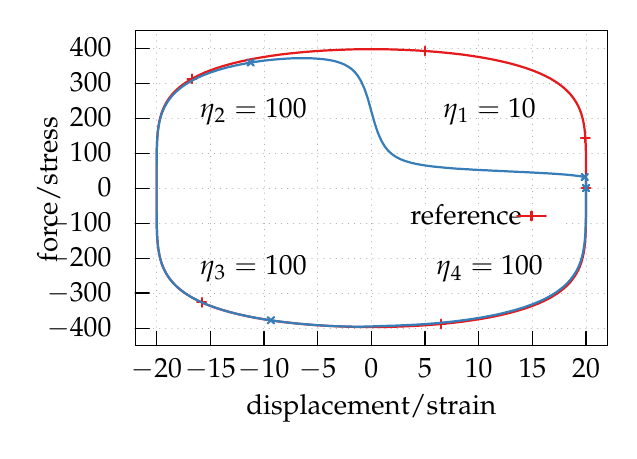
\begin{tikzpicture}[gnuplot]
%% generated with GNUPLOT 5.2p7 (Lua 5.3; terminal rev. Nov 2018, script rev. 107)
%% 08/29/2020 16:55:16
\path (0.000,0.000) rectangle (6.000,4.000);
\gpcolor{color=gp lt color axes}
\gpsetlinetype{gp lt axes}
\gpsetdashtype{gp dt axes}
\gpsetlinewidth{0.50}
\draw[gp path] (0.000,0.222)--(5.999,0.222);
\gpcolor{color=gp lt color border}
\gpsetlinetype{gp lt border}
\gpsetdashtype{gp dt solid}
\gpsetlinewidth{1.00}
\draw[gp path] (0.000,0.222)--(0.180,0.222);
\node[gp node right] at (-0.184,0.222) {$-400$};
\gpcolor{color=gp lt color axes}
\gpsetlinetype{gp lt axes}
\gpsetdashtype{gp dt axes}
\gpsetlinewidth{0.50}
\draw[gp path] (0.000,0.667)--(5.999,0.667);
\gpcolor{color=gp lt color border}
\gpsetlinetype{gp lt border}
\gpsetdashtype{gp dt solid}
\gpsetlinewidth{1.00}
\draw[gp path] (0.000,0.667)--(0.180,0.667);
\node[gp node right] at (-0.184,0.667) {$-300$};
\gpcolor{color=gp lt color axes}
\gpsetlinetype{gp lt axes}
\gpsetdashtype{gp dt axes}
\gpsetlinewidth{0.50}
\draw[gp path] (0.000,1.111)--(5.999,1.111);
\gpcolor{color=gp lt color border}
\gpsetlinetype{gp lt border}
\gpsetdashtype{gp dt solid}
\gpsetlinewidth{1.00}
\draw[gp path] (0.000,1.111)--(0.180,1.111);
\node[gp node right] at (-0.184,1.111) {$-200$};
\gpcolor{color=gp lt color axes}
\gpsetlinetype{gp lt axes}
\gpsetdashtype{gp dt axes}
\gpsetlinewidth{0.50}
\draw[gp path] (0.000,1.555)--(3.379,1.555);
\draw[gp path] (5.399,1.555)--(5.999,1.555);
\gpcolor{color=gp lt color border}
\gpsetlinetype{gp lt border}
\gpsetdashtype{gp dt solid}
\gpsetlinewidth{1.00}
\draw[gp path] (0.000,1.555)--(0.180,1.555);
\node[gp node right] at (-0.184,1.555) {$-100$};
\gpcolor{color=gp lt color axes}
\gpsetlinetype{gp lt axes}
\gpsetdashtype{gp dt axes}
\gpsetlinewidth{0.50}
\draw[gp path] (0.000,2.000)--(5.999,2.000);
\gpcolor{color=gp lt color border}
\gpsetlinetype{gp lt border}
\gpsetdashtype{gp dt solid}
\gpsetlinewidth{1.00}
\draw[gp path] (0.000,2.000)--(0.180,2.000);
\node[gp node right] at (-0.184,2.000) {$0$};
\gpcolor{color=gp lt color axes}
\gpsetlinetype{gp lt axes}
\gpsetdashtype{gp dt axes}
\gpsetlinewidth{0.50}
\draw[gp path] (0.000,2.444)--(5.999,2.444);
\gpcolor{color=gp lt color border}
\gpsetlinetype{gp lt border}
\gpsetdashtype{gp dt solid}
\gpsetlinewidth{1.00}
\draw[gp path] (0.000,2.444)--(0.180,2.444);
\node[gp node right] at (-0.184,2.444) {$100$};
\gpcolor{color=gp lt color axes}
\gpsetlinetype{gp lt axes}
\gpsetdashtype{gp dt axes}
\gpsetlinewidth{0.50}
\draw[gp path] (0.000,2.888)--(5.999,2.888);
\gpcolor{color=gp lt color border}
\gpsetlinetype{gp lt border}
\gpsetdashtype{gp dt solid}
\gpsetlinewidth{1.00}
\draw[gp path] (0.000,2.888)--(0.180,2.888);
\node[gp node right] at (-0.184,2.888) {$200$};
\gpcolor{color=gp lt color axes}
\gpsetlinetype{gp lt axes}
\gpsetdashtype{gp dt axes}
\gpsetlinewidth{0.50}
\draw[gp path] (0.000,3.333)--(5.999,3.333);
\gpcolor{color=gp lt color border}
\gpsetlinetype{gp lt border}
\gpsetdashtype{gp dt solid}
\gpsetlinewidth{1.00}
\draw[gp path] (0.000,3.333)--(0.180,3.333);
\node[gp node right] at (-0.184,3.333) {$300$};
\gpcolor{color=gp lt color axes}
\gpsetlinetype{gp lt axes}
\gpsetdashtype{gp dt axes}
\gpsetlinewidth{0.50}
\draw[gp path] (0.000,3.777)--(5.999,3.777);
\gpcolor{color=gp lt color border}
\gpsetlinetype{gp lt border}
\gpsetdashtype{gp dt solid}
\gpsetlinewidth{1.00}
\draw[gp path] (0.000,3.777)--(0.180,3.777);
\node[gp node right] at (-0.184,3.777) {$400$};
\gpcolor{color=gp lt color axes}
\gpsetlinetype{gp lt axes}
\gpsetdashtype{gp dt axes}
\gpsetlinewidth{0.50}
\draw[gp path] (0.273,0.000)--(0.273,3.999);
\gpcolor{color=gp lt color border}
\gpsetlinetype{gp lt border}
\gpsetdashtype{gp dt solid}
\gpsetlinewidth{1.00}
\draw[gp path] (0.273,0.000)--(0.273,0.180);
\node[gp node center] at (0.273,-0.308) {$-20$};
\gpcolor{color=gp lt color axes}
\gpsetlinetype{gp lt axes}
\gpsetdashtype{gp dt axes}
\gpsetlinewidth{0.50}
\draw[gp path] (0.954,0.000)--(0.954,3.999);
\gpcolor{color=gp lt color border}
\gpsetlinetype{gp lt border}
\gpsetdashtype{gp dt solid}
\gpsetlinewidth{1.00}
\draw[gp path] (0.954,0.000)--(0.954,0.180);
\node[gp node center] at (0.954,-0.308) {$-15$};
\gpcolor{color=gp lt color axes}
\gpsetlinetype{gp lt axes}
\gpsetdashtype{gp dt axes}
\gpsetlinewidth{0.50}
\draw[gp path] (1.636,0.000)--(1.636,3.999);
\gpcolor{color=gp lt color border}
\gpsetlinetype{gp lt border}
\gpsetdashtype{gp dt solid}
\gpsetlinewidth{1.00}
\draw[gp path] (1.636,0.000)--(1.636,0.180);
\node[gp node center] at (1.636,-0.308) {$-10$};
\gpcolor{color=gp lt color axes}
\gpsetlinetype{gp lt axes}
\gpsetdashtype{gp dt axes}
\gpsetlinewidth{0.50}
\draw[gp path] (2.318,0.000)--(2.318,3.999);
\gpcolor{color=gp lt color border}
\gpsetlinetype{gp lt border}
\gpsetdashtype{gp dt solid}
\gpsetlinewidth{1.00}
\draw[gp path] (2.318,0.000)--(2.318,0.180);
\node[gp node center] at (2.318,-0.308) {$-5$};
\gpcolor{color=gp lt color axes}
\gpsetlinetype{gp lt axes}
\gpsetdashtype{gp dt axes}
\gpsetlinewidth{0.50}
\draw[gp path] (3.000,0.000)--(3.000,3.999);
\gpcolor{color=gp lt color border}
\gpsetlinetype{gp lt border}
\gpsetdashtype{gp dt solid}
\gpsetlinewidth{1.00}
\draw[gp path] (3.000,0.000)--(3.000,0.180);
\node[gp node center] at (3.000,-0.308) {$0$};
\gpcolor{color=gp lt color axes}
\gpsetlinetype{gp lt axes}
\gpsetdashtype{gp dt axes}
\gpsetlinewidth{0.50}
\draw[gp path] (3.681,0.000)--(3.681,1.492);
\draw[gp path] (3.681,1.800)--(3.681,3.999);
\gpcolor{color=gp lt color border}
\gpsetlinetype{gp lt border}
\gpsetdashtype{gp dt solid}
\gpsetlinewidth{1.00}
\draw[gp path] (3.681,0.000)--(3.681,0.180);
\node[gp node center] at (3.681,-0.308) {$5$};
\gpcolor{color=gp lt color axes}
\gpsetlinetype{gp lt axes}
\gpsetdashtype{gp dt axes}
\gpsetlinewidth{0.50}
\draw[gp path] (4.363,0.000)--(4.363,1.492);
\draw[gp path] (4.363,1.800)--(4.363,3.999);
\gpcolor{color=gp lt color border}
\gpsetlinetype{gp lt border}
\gpsetdashtype{gp dt solid}
\gpsetlinewidth{1.00}
\draw[gp path] (4.363,0.000)--(4.363,0.180);
\node[gp node center] at (4.363,-0.308) {$10$};
\gpcolor{color=gp lt color axes}
\gpsetlinetype{gp lt axes}
\gpsetdashtype{gp dt axes}
\gpsetlinewidth{0.50}
\draw[gp path] (5.045,0.000)--(5.045,1.492);
\draw[gp path] (5.045,1.800)--(5.045,3.999);
\gpcolor{color=gp lt color border}
\gpsetlinetype{gp lt border}
\gpsetdashtype{gp dt solid}
\gpsetlinewidth{1.00}
\draw[gp path] (5.045,0.000)--(5.045,0.180);
\node[gp node center] at (5.045,-0.308) {$15$};
\gpcolor{color=gp lt color axes}
\gpsetlinetype{gp lt axes}
\gpsetdashtype{gp dt axes}
\gpsetlinewidth{0.50}
\draw[gp path] (5.726,0.000)--(5.726,3.999);
\gpcolor{color=gp lt color border}
\gpsetlinetype{gp lt border}
\gpsetdashtype{gp dt solid}
\gpsetlinewidth{1.00}
\draw[gp path] (5.726,0.000)--(5.726,0.180);
\node[gp node center] at (5.726,-0.308) {$20$};
\draw[gp path] (0.000,3.999)--(0.000,0.000)--(5.999,0.000)--(5.999,3.999)--cycle;
\node[gp node center] at (4.499,2.999) {$\eta_1=10$};
\node[gp node center] at (1.500,2.999) {$\eta_2=100$};
\node[gp node center] at (1.500,1.000) {$\eta_3=100$};
\node[gp node center] at (4.499,1.000) {$\eta_4=100$};
\node[gp node center,rotate=-270] at (-1.074,1.999) {force/stress};
\node[gp node center] at (2.999,-0.769) {displacement/strain};
\gpcolor{rgb color={0.894,0.102,0.110}}
\gpsetlinewidth{2.00}
\draw[gp path] (5.726,2.000)--(5.726,1.730)--(5.725,1.558)--(5.723,1.480)--(5.721,1.416)%
  --(5.718,1.362)--(5.714,1.314)--(5.710,1.271)--(5.705,1.231)--(5.699,1.194)--(5.693,1.159)%
  --(5.686,1.127)--(5.678,1.097)--(5.670,1.068)--(5.661,1.040)--(5.651,1.014)--(5.641,0.988)%
  --(5.630,0.964)--(5.618,0.941)--(5.606,0.918)--(5.593,0.897)--(5.579,0.876)--(5.565,0.855)%
  --(5.550,0.836)--(5.535,0.817)--(5.519,0.798)--(5.502,0.780)--(5.485,0.763)--(5.467,0.746)%
  --(5.448,0.729)--(5.429,0.713)--(5.409,0.697)--(5.389,0.682)--(5.368,0.667)--(5.347,0.653)%
  --(5.324,0.639)--(5.302,0.625)--(5.279,0.611)--(5.255,0.598)--(5.230,0.586)--(5.206,0.573)%
  --(5.180,0.561)--(5.154,0.549)--(5.128,0.537)--(5.101,0.526)--(5.073,0.515)--(5.045,0.504)%
  --(5.016,0.494)--(4.987,0.483)--(4.958,0.473)--(4.928,0.464)--(4.897,0.454)--(4.866,0.445)%
  --(4.835,0.436)--(4.803,0.427)--(4.770,0.418)--(4.738,0.410)--(4.704,0.402)--(4.671,0.394)%
  --(4.637,0.386)--(4.602,0.379)--(4.567,0.371)--(4.532,0.364)--(4.497,0.357)--(4.461,0.351)%
  --(4.424,0.344)--(4.388,0.338)--(4.351,0.332)--(4.313,0.326)--(4.275,0.320)--(4.237,0.315)%
  --(4.199,0.309)--(4.161,0.304)--(4.122,0.299)--(4.082,0.295)--(4.043,0.290)--(4.003,0.286)%
  --(3.963,0.282)--(3.923,0.278)--(3.883,0.274)--(3.842,0.270)--(3.801,0.267)--(3.760,0.264)%
  --(3.719,0.260)--(3.678,0.258)--(3.636,0.255)--(3.594,0.252)--(3.552,0.250)--(3.510,0.248)%
  --(3.468,0.246)--(3.426,0.244)--(3.384,0.242)--(3.341,0.241)--(3.299,0.239)--(3.256,0.238)%
  --(3.213,0.237)--(3.171,0.237)--(3.128,0.236)--(3.085,0.236)--(3.042,0.235)--(2.999,0.235)%
  --(2.957,0.235)--(2.914,0.236)--(2.871,0.236)--(2.828,0.237)--(2.786,0.237)--(2.743,0.238)%
  --(2.700,0.239)--(2.658,0.241)--(2.615,0.242)--(2.573,0.244)--(2.531,0.246)--(2.489,0.248)%
  --(2.447,0.250)--(2.405,0.252)--(2.363,0.255)--(2.321,0.258)--(2.280,0.260)--(2.239,0.264)%
  --(2.198,0.267)--(2.157,0.270)--(2.116,0.274)--(2.076,0.278)--(2.036,0.282)--(1.996,0.286)%
  --(1.956,0.290)--(1.917,0.295)--(1.877,0.299)--(1.838,0.304)--(1.800,0.309)--(1.762,0.315)%
  --(1.724,0.320)--(1.686,0.326)--(1.648,0.332)--(1.611,0.338)--(1.575,0.344)--(1.538,0.351)%
  --(1.502,0.357)--(1.467,0.364)--(1.432,0.371)--(1.397,0.379)--(1.362,0.386)--(1.328,0.394)%
  --(1.295,0.402)--(1.261,0.410)--(1.229,0.418)--(1.196,0.427)--(1.164,0.436)--(1.133,0.445)%
  --(1.102,0.454)--(1.071,0.464)--(1.041,0.473)--(1.012,0.483)--(0.983,0.494)--(0.954,0.504)%
  --(0.926,0.515)--(0.898,0.526)--(0.871,0.537)--(0.845,0.549)--(0.819,0.561)--(0.793,0.573)%
  --(0.769,0.586)--(0.744,0.598)--(0.720,0.611)--(0.697,0.625)--(0.675,0.639)--(0.652,0.653)%
  --(0.631,0.667)--(0.610,0.682)--(0.590,0.697)--(0.570,0.713)--(0.551,0.729)--(0.532,0.746)%
  --(0.514,0.763)--(0.497,0.780)--(0.480,0.798)--(0.464,0.817)--(0.449,0.836)--(0.434,0.855)%
  --(0.420,0.876)--(0.406,0.897)--(0.393,0.918)--(0.381,0.941)--(0.369,0.964)--(0.358,0.988)%
  --(0.348,1.014)--(0.338,1.040)--(0.329,1.068)--(0.321,1.097)--(0.313,1.127)--(0.306,1.159)%
  --(0.300,1.194)--(0.294,1.231)--(0.289,1.271)--(0.285,1.314)--(0.281,1.362)--(0.278,1.416)%
  --(0.276,1.480)--(0.274,1.558)--(0.273,1.730)--(0.273,1.999)--(0.273,2.269)--(0.274,2.441)%
  --(0.276,2.519)--(0.278,2.583)--(0.281,2.637)--(0.285,2.685)--(0.289,2.728)--(0.294,2.768)%
  --(0.300,2.805)--(0.306,2.840)--(0.313,2.872)--(0.321,2.902)--(0.329,2.931)--(0.338,2.959)%
  --(0.348,2.985)--(0.358,3.011)--(0.369,3.035)--(0.381,3.058)--(0.393,3.081)--(0.406,3.102)%
  --(0.420,3.123)--(0.434,3.144)--(0.449,3.163)--(0.464,3.182)--(0.480,3.201)--(0.497,3.219)%
  --(0.514,3.236)--(0.532,3.253)--(0.551,3.270)--(0.570,3.286)--(0.590,3.302)--(0.610,3.317)%
  --(0.631,3.332)--(0.652,3.346)--(0.675,3.360)--(0.697,3.374)--(0.720,3.388)--(0.744,3.401)%
  --(0.769,3.413)--(0.793,3.426)--(0.819,3.438)--(0.845,3.450)--(0.871,3.462)--(0.898,3.473)%
  --(0.926,3.484)--(0.954,3.495)--(0.983,3.505)--(1.012,3.516)--(1.041,3.526)--(1.071,3.535)%
  --(1.102,3.545)--(1.133,3.554)--(1.164,3.563)--(1.196,3.572)--(1.229,3.581)--(1.261,3.589)%
  --(1.295,3.597)--(1.328,3.605)--(1.362,3.613)--(1.397,3.620)--(1.432,3.628)--(1.467,3.635)%
  --(1.502,3.642)--(1.538,3.648)--(1.575,3.655)--(1.611,3.661)--(1.648,3.667)--(1.686,3.673)%
  --(1.724,3.679)--(1.762,3.684)--(1.800,3.690)--(1.838,3.695)--(1.877,3.700)--(1.917,3.704)%
  --(1.956,3.709)--(1.996,3.713)--(2.036,3.717)--(2.076,3.721)--(2.116,3.725)--(2.157,3.729)%
  --(2.198,3.732)--(2.239,3.735)--(2.280,3.739)--(2.321,3.741)--(2.363,3.744)--(2.405,3.747)%
  --(2.447,3.749)--(2.489,3.751)--(2.531,3.753)--(2.573,3.755)--(2.615,3.757)--(2.658,3.758)%
  --(2.700,3.760)--(2.743,3.761)--(2.786,3.762)--(2.828,3.762)--(2.871,3.763)--(2.914,3.763)%
  --(2.957,3.764)--(2.999,3.764)--(3.042,3.764)--(3.085,3.763)--(3.128,3.763)--(3.171,3.762)%
  --(3.213,3.762)--(3.256,3.761)--(3.299,3.760)--(3.341,3.758)--(3.384,3.757)--(3.426,3.755)%
  --(3.468,3.753)--(3.510,3.751)--(3.552,3.749)--(3.594,3.747)--(3.636,3.744)--(3.678,3.741)%
  --(3.719,3.739)--(3.760,3.735)--(3.801,3.732)--(3.842,3.729)--(3.883,3.725)--(3.923,3.721)%
  --(3.963,3.717)--(4.003,3.713)--(4.043,3.709)--(4.082,3.704)--(4.122,3.700)--(4.161,3.695)%
  --(4.199,3.690)--(4.237,3.684)--(4.275,3.679)--(4.313,3.673)--(4.351,3.667)--(4.388,3.661)%
  --(4.424,3.655)--(4.461,3.648)--(4.497,3.642)--(4.532,3.635)--(4.567,3.628)--(4.602,3.620)%
  --(4.637,3.613)--(4.671,3.605)--(4.704,3.597)--(4.738,3.589)--(4.770,3.581)--(4.803,3.572)%
  --(4.835,3.563)--(4.866,3.554)--(4.897,3.545)--(4.928,3.535)--(4.958,3.526)--(4.987,3.516)%
  --(5.016,3.505)--(5.045,3.495)--(5.073,3.484)--(5.101,3.473)--(5.128,3.462)--(5.154,3.450)%
  --(5.180,3.438)--(5.206,3.426)--(5.230,3.413)--(5.255,3.401)--(5.279,3.388)--(5.302,3.374)%
  --(5.324,3.360)--(5.347,3.346)--(5.368,3.332)--(5.389,3.317)--(5.409,3.302)--(5.429,3.286)%
  --(5.448,3.270)--(5.467,3.253)--(5.485,3.236)--(5.502,3.219)--(5.519,3.201)--(5.535,3.182)%
  --(5.550,3.163)--(5.565,3.144)--(5.579,3.123)--(5.593,3.102)--(5.606,3.081)--(5.618,3.058)%
  --(5.630,3.035)--(5.641,3.011)--(5.651,2.985)--(5.661,2.959)--(5.670,2.931)--(5.678,2.902)%
  --(5.686,2.872)--(5.693,2.840)--(5.699,2.805)--(5.705,2.768)--(5.710,2.728)--(5.714,2.685)%
  --(5.718,2.637)--(5.721,2.583)--(5.723,2.519)--(5.725,2.441)--(5.726,2.269)--(5.726,1.999);
\gpsetpointsize{4.00}
\gppoint{gp mark 1}{(5.726,2.000)}
\gppoint{gp mark 1}{(3.883,0.274)}
\gppoint{gp mark 1}{(0.845,0.549)}
\gppoint{gp mark 1}{(0.720,3.388)}
\gppoint{gp mark 1}{(3.678,3.741)}
\gppoint{gp mark 1}{(5.718,2.637)}
\gpcolor{rgb color={0.216,0.494,0.722}}
\draw[gp path] (5.726,2.000)--(5.726,1.815)--(5.725,1.656)--(5.723,1.567)--(5.721,1.494)%
  --(5.718,1.431)--(5.714,1.377)--(5.710,1.329)--(5.705,1.285)--(5.699,1.244)--(5.693,1.207)%
  --(5.686,1.172)--(5.678,1.139)--(5.670,1.108)--(5.661,1.079)--(5.651,1.051)--(5.641,1.025)%
  --(5.630,0.999)--(5.618,0.975)--(5.606,0.951)--(5.593,0.928)--(5.579,0.907)--(5.565,0.885)%
  --(5.550,0.865)--(5.535,0.845)--(5.519,0.826)--(5.502,0.808)--(5.485,0.790)--(5.467,0.772)%
  --(5.448,0.755)--(5.429,0.738)--(5.409,0.722)--(5.389,0.707)--(5.368,0.691)--(5.347,0.676)%
  --(5.324,0.662)--(5.302,0.648)--(5.279,0.634)--(5.255,0.621)--(5.230,0.607)--(5.206,0.595)%
  --(5.180,0.582)--(5.154,0.570)--(5.128,0.558)--(5.101,0.547)--(5.073,0.535)--(5.045,0.524)%
  --(5.016,0.514)--(4.987,0.503)--(4.958,0.493)--(4.928,0.483)--(4.897,0.473)--(4.866,0.464)%
  --(4.835,0.455)--(4.803,0.446)--(4.770,0.437)--(4.738,0.428)--(4.704,0.420)--(4.671,0.412)%
  --(4.637,0.404)--(4.602,0.396)--(4.567,0.389)--(4.532,0.382)--(4.497,0.375)--(4.461,0.368)%
  --(4.424,0.361)--(4.388,0.355)--(4.351,0.349)--(4.313,0.343)--(4.275,0.337)--(4.237,0.331)%
  --(4.199,0.326)--(4.161,0.321)--(4.122,0.316)--(4.082,0.311)--(4.043,0.306)--(4.003,0.302)%
  --(3.963,0.298)--(3.923,0.294)--(3.883,0.290)--(3.842,0.286)--(3.801,0.282)--(3.760,0.279)%
  --(3.719,0.276)--(3.678,0.273)--(3.636,0.270)--(3.594,0.267)--(3.552,0.265)--(3.510,0.263)%
  --(3.468,0.261)--(3.426,0.259)--(3.384,0.257)--(3.341,0.255)--(3.299,0.253)--(3.256,0.252)%
  --(3.213,0.251)--(3.171,0.249)--(3.128,0.248)--(3.085,0.246)--(3.042,0.245)--(2.999,0.243)%
  --(2.957,0.242)--(2.914,0.241)--(2.871,0.240)--(2.828,0.240)--(2.786,0.240)--(2.743,0.241)%
  --(2.700,0.242)--(2.658,0.243)--(2.615,0.244)--(2.573,0.246)--(2.531,0.247)--(2.489,0.249)%
  --(2.447,0.251)--(2.405,0.253)--(2.363,0.256)--(2.321,0.259)--(2.280,0.261)--(2.239,0.264)%
  --(2.198,0.268)--(2.157,0.271)--(2.116,0.275)--(2.076,0.278)--(2.036,0.282)--(1.996,0.287)%
  --(1.956,0.291)--(1.917,0.295)--(1.877,0.300)--(1.838,0.305)--(1.800,0.310)--(1.762,0.315)%
  --(1.724,0.321)--(1.686,0.327)--(1.648,0.332)--(1.611,0.338)--(1.575,0.345)--(1.538,0.351)%
  --(1.502,0.358)--(1.467,0.365)--(1.432,0.372)--(1.397,0.379)--(1.362,0.387)--(1.328,0.394)%
  --(1.295,0.402)--(1.261,0.410)--(1.229,0.419)--(1.196,0.427)--(1.164,0.436)--(1.133,0.445)%
  --(1.102,0.455)--(1.071,0.464)--(1.041,0.474)--(1.012,0.484)--(0.983,0.494)--(0.954,0.505)%
  --(0.926,0.515)--(0.898,0.526)--(0.871,0.538)--(0.845,0.549)--(0.819,0.561)--(0.793,0.573)%
  --(0.769,0.586)--(0.744,0.599)--(0.720,0.612)--(0.697,0.625)--(0.675,0.639)--(0.652,0.653)%
  --(0.631,0.668)--(0.610,0.683)--(0.590,0.698)--(0.570,0.714)--(0.551,0.730)--(0.532,0.746)%
  --(0.514,0.763)--(0.497,0.781)--(0.480,0.799)--(0.464,0.817)--(0.449,0.836)--(0.434,0.856)%
  --(0.420,0.876)--(0.406,0.897)--(0.393,0.919)--(0.381,0.941)--(0.369,0.965)--(0.358,0.989)%
  --(0.348,1.014)--(0.338,1.041)--(0.329,1.068)--(0.321,1.097)--(0.313,1.128)--(0.306,1.160)%
  --(0.300,1.195)--(0.294,1.232)--(0.289,1.271)--(0.285,1.315)--(0.281,1.363)--(0.278,1.418)%
  --(0.276,1.481)--(0.274,1.559)--(0.273,1.732)--(0.273,1.999)--(0.273,2.266)--(0.274,2.437)%
  --(0.276,2.513)--(0.278,2.575)--(0.281,2.629)--(0.285,2.676)--(0.289,2.719)--(0.294,2.758)%
  --(0.300,2.794)--(0.306,2.828)--(0.313,2.860)--(0.321,2.890)--(0.329,2.918)--(0.338,2.946)%
  --(0.348,2.972)--(0.358,2.996)--(0.369,3.020)--(0.381,3.043)--(0.393,3.065)--(0.406,3.086)%
  --(0.420,3.107)--(0.434,3.127)--(0.449,3.146)--(0.464,3.165)--(0.480,3.183)--(0.497,3.200)%
  --(0.514,3.217)--(0.532,3.234)--(0.551,3.250)--(0.570,3.266)--(0.590,3.281)--(0.610,3.296)%
  --(0.631,3.310)--(0.652,3.324)--(0.675,3.338)--(0.697,3.351)--(0.720,3.364)--(0.744,3.377)%
  --(0.769,3.389)--(0.793,3.401)--(0.819,3.413)--(0.845,3.424)--(0.871,3.435)--(0.898,3.446)%
  --(0.926,3.457)--(0.954,3.467)--(0.983,3.477)--(1.012,3.486)--(1.041,3.496)--(1.071,3.505)%
  --(1.102,3.514)--(1.133,3.522)--(1.164,3.531)--(1.196,3.539)--(1.229,3.546)--(1.261,3.554)%
  --(1.295,3.561)--(1.328,3.568)--(1.362,3.575)--(1.397,3.581)--(1.432,3.588)--(1.467,3.594)%
  --(1.502,3.599)--(1.538,3.605)--(1.575,3.610)--(1.611,3.615)--(1.648,3.620)--(1.686,3.624)%
  --(1.724,3.628)--(1.762,3.632)--(1.800,3.635)--(1.838,3.638)--(1.877,3.641)--(1.917,3.644)%
  --(1.956,3.646)--(1.996,3.648)--(2.036,3.649)--(2.076,3.650)--(2.116,3.650)--(2.157,3.650)%
  --(2.198,3.649)--(2.239,3.648)--(2.280,3.646)--(2.321,3.643)--(2.363,3.640)--(2.405,3.635)%
  --(2.447,3.629)--(2.489,3.622)--(2.531,3.613)--(2.573,3.601)--(2.615,3.587)--(2.658,3.569)%
  --(2.700,3.546)--(2.743,3.517)--(2.786,3.478)--(2.828,3.426)--(2.871,3.355)--(2.914,3.258)%
  --(2.957,3.130)--(2.999,2.978)--(3.042,2.826)--(3.085,2.697)--(3.128,2.600)--(3.171,2.528)%
  --(3.213,2.475)--(3.256,2.436)--(3.299,2.405)--(3.341,2.381)--(3.384,2.361)--(3.426,2.345)%
  --(3.468,2.332)--(3.510,2.320)--(3.552,2.311)--(3.594,2.302)--(3.636,2.295)--(3.678,2.288)%
  --(3.719,2.282)--(3.760,2.277)--(3.801,2.272)--(3.842,2.268)--(3.883,2.264)--(3.923,2.260)%
  --(3.963,2.256)--(4.003,2.253)--(4.043,2.250)--(4.082,2.247)--(4.122,2.245)--(4.161,2.242)%
  --(4.199,2.240)--(4.237,2.238)--(4.275,2.235)--(4.313,2.233)--(4.351,2.231)--(4.388,2.229)%
  --(4.424,2.227)--(4.461,2.226)--(4.497,2.224)--(4.532,2.222)--(4.567,2.220)--(4.602,2.219)%
  --(4.637,2.217)--(4.671,2.216)--(4.704,2.214)--(4.738,2.212)--(4.770,2.211)--(4.803,2.209)%
  --(4.835,2.208)--(4.866,2.206)--(4.897,2.205)--(4.928,2.204)--(4.958,2.202)--(4.987,2.201)%
  --(5.016,2.199)--(5.045,2.198)--(5.073,2.196)--(5.101,2.195)--(5.128,2.193)--(5.154,2.192)%
  --(5.180,2.190)--(5.206,2.189)--(5.230,2.188)--(5.255,2.186)--(5.279,2.185)--(5.302,2.183)%
  --(5.324,2.182)--(5.347,2.180)--(5.368,2.179)--(5.389,2.177)--(5.409,2.176)--(5.429,2.174)%
  --(5.448,2.173)--(5.467,2.171)--(5.485,2.169)--(5.502,2.168)--(5.519,2.166)--(5.535,2.165)%
  --(5.550,2.163)--(5.565,2.162)--(5.579,2.160)--(5.593,2.158)--(5.606,2.157)--(5.618,2.155)%
  --(5.630,2.153)--(5.641,2.152)--(5.651,2.150)--(5.661,2.149)--(5.670,2.147)--(5.678,2.146)%
  --(5.686,2.144)--(5.693,2.143)--(5.699,2.142)--(5.705,2.141)--(5.710,2.141)--(5.714,2.141)%
  --(5.718,2.142)--(5.721,2.143)--(5.723,2.146)--(5.725,2.149)--(5.726,2.115)--(5.726,1.999);
\gppoint{gp mark 2}{(5.726,2.000)}
\gppoint{gp mark 2}{(1.724,0.321)}
\gppoint{gp mark 2}{(1.467,3.594)}
\gppoint{gp mark 2}{(5.710,2.141)}
\gpfill{color=gpbgfillcolor} (3.379,1.492)--(5.399,1.492)--(5.399,1.800)--(3.379,1.800)--cycle;
\gpcolor{color=gp lt color border}
\node[gp node left] at (3.379,1.646) {reference};
\gpcolor{rgb color={0.894,0.102,0.110}}
\draw[gp path] (4.851,1.646)--(5.215,1.646);
\gppoint{gp mark 1}{(5.033,1.646)}
\gpcolor{color=gp lt color border}
\gpsetlinewidth{1.00}
\draw[gp path] (0.000,3.999)--(0.000,0.000)--(5.999,0.000)--(5.999,3.999)--cycle;
%% coordinates of the plot area
\gpdefrectangularnode{gp plot 1}{\pgfpoint{0.000cm}{0.000cm}}{\pgfpoint{5.999cm}{3.999cm}}
\end{tikzpicture}
%% gnuplot variables

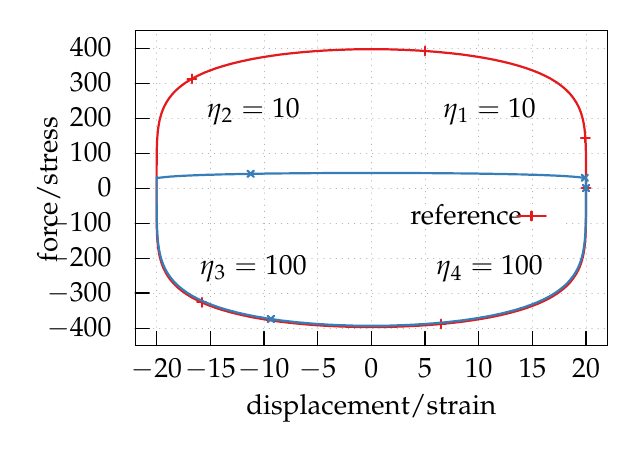
\begin{tikzpicture}[gnuplot]
%% generated with GNUPLOT 5.2p7 (Lua 5.3; terminal rev. Nov 2018, script rev. 107)
%% 08/29/2020 16:55:16
\path (0.000,0.000) rectangle (6.000,4.000);
\gpcolor{color=gp lt color axes}
\gpsetlinetype{gp lt axes}
\gpsetdashtype{gp dt axes}
\gpsetlinewidth{0.50}
\draw[gp path] (0.000,0.222)--(5.999,0.222);
\gpcolor{color=gp lt color border}
\gpsetlinetype{gp lt border}
\gpsetdashtype{gp dt solid}
\gpsetlinewidth{1.00}
\draw[gp path] (0.000,0.222)--(0.180,0.222);
\node[gp node right] at (-0.184,0.222) {$-400$};
\gpcolor{color=gp lt color axes}
\gpsetlinetype{gp lt axes}
\gpsetdashtype{gp dt axes}
\gpsetlinewidth{0.50}
\draw[gp path] (0.000,0.667)--(5.999,0.667);
\gpcolor{color=gp lt color border}
\gpsetlinetype{gp lt border}
\gpsetdashtype{gp dt solid}
\gpsetlinewidth{1.00}
\draw[gp path] (0.000,0.667)--(0.180,0.667);
\node[gp node right] at (-0.184,0.667) {$-300$};
\gpcolor{color=gp lt color axes}
\gpsetlinetype{gp lt axes}
\gpsetdashtype{gp dt axes}
\gpsetlinewidth{0.50}
\draw[gp path] (0.000,1.111)--(5.999,1.111);
\gpcolor{color=gp lt color border}
\gpsetlinetype{gp lt border}
\gpsetdashtype{gp dt solid}
\gpsetlinewidth{1.00}
\draw[gp path] (0.000,1.111)--(0.180,1.111);
\node[gp node right] at (-0.184,1.111) {$-200$};
\gpcolor{color=gp lt color axes}
\gpsetlinetype{gp lt axes}
\gpsetdashtype{gp dt axes}
\gpsetlinewidth{0.50}
\draw[gp path] (0.000,1.555)--(3.379,1.555);
\draw[gp path] (5.399,1.555)--(5.999,1.555);
\gpcolor{color=gp lt color border}
\gpsetlinetype{gp lt border}
\gpsetdashtype{gp dt solid}
\gpsetlinewidth{1.00}
\draw[gp path] (0.000,1.555)--(0.180,1.555);
\node[gp node right] at (-0.184,1.555) {$-100$};
\gpcolor{color=gp lt color axes}
\gpsetlinetype{gp lt axes}
\gpsetdashtype{gp dt axes}
\gpsetlinewidth{0.50}
\draw[gp path] (0.000,2.000)--(5.999,2.000);
\gpcolor{color=gp lt color border}
\gpsetlinetype{gp lt border}
\gpsetdashtype{gp dt solid}
\gpsetlinewidth{1.00}
\draw[gp path] (0.000,2.000)--(0.180,2.000);
\node[gp node right] at (-0.184,2.000) {$0$};
\gpcolor{color=gp lt color axes}
\gpsetlinetype{gp lt axes}
\gpsetdashtype{gp dt axes}
\gpsetlinewidth{0.50}
\draw[gp path] (0.000,2.444)--(5.999,2.444);
\gpcolor{color=gp lt color border}
\gpsetlinetype{gp lt border}
\gpsetdashtype{gp dt solid}
\gpsetlinewidth{1.00}
\draw[gp path] (0.000,2.444)--(0.180,2.444);
\node[gp node right] at (-0.184,2.444) {$100$};
\gpcolor{color=gp lt color axes}
\gpsetlinetype{gp lt axes}
\gpsetdashtype{gp dt axes}
\gpsetlinewidth{0.50}
\draw[gp path] (0.000,2.888)--(5.999,2.888);
\gpcolor{color=gp lt color border}
\gpsetlinetype{gp lt border}
\gpsetdashtype{gp dt solid}
\gpsetlinewidth{1.00}
\draw[gp path] (0.000,2.888)--(0.180,2.888);
\node[gp node right] at (-0.184,2.888) {$200$};
\gpcolor{color=gp lt color axes}
\gpsetlinetype{gp lt axes}
\gpsetdashtype{gp dt axes}
\gpsetlinewidth{0.50}
\draw[gp path] (0.000,3.333)--(5.999,3.333);
\gpcolor{color=gp lt color border}
\gpsetlinetype{gp lt border}
\gpsetdashtype{gp dt solid}
\gpsetlinewidth{1.00}
\draw[gp path] (0.000,3.333)--(0.180,3.333);
\node[gp node right] at (-0.184,3.333) {$300$};
\gpcolor{color=gp lt color axes}
\gpsetlinetype{gp lt axes}
\gpsetdashtype{gp dt axes}
\gpsetlinewidth{0.50}
\draw[gp path] (0.000,3.777)--(5.999,3.777);
\gpcolor{color=gp lt color border}
\gpsetlinetype{gp lt border}
\gpsetdashtype{gp dt solid}
\gpsetlinewidth{1.00}
\draw[gp path] (0.000,3.777)--(0.180,3.777);
\node[gp node right] at (-0.184,3.777) {$400$};
\gpcolor{color=gp lt color axes}
\gpsetlinetype{gp lt axes}
\gpsetdashtype{gp dt axes}
\gpsetlinewidth{0.50}
\draw[gp path] (0.273,0.000)--(0.273,3.999);
\gpcolor{color=gp lt color border}
\gpsetlinetype{gp lt border}
\gpsetdashtype{gp dt solid}
\gpsetlinewidth{1.00}
\draw[gp path] (0.273,0.000)--(0.273,0.180);
\node[gp node center] at (0.273,-0.308) {$-20$};
\gpcolor{color=gp lt color axes}
\gpsetlinetype{gp lt axes}
\gpsetdashtype{gp dt axes}
\gpsetlinewidth{0.50}
\draw[gp path] (0.954,0.000)--(0.954,3.999);
\gpcolor{color=gp lt color border}
\gpsetlinetype{gp lt border}
\gpsetdashtype{gp dt solid}
\gpsetlinewidth{1.00}
\draw[gp path] (0.954,0.000)--(0.954,0.180);
\node[gp node center] at (0.954,-0.308) {$-15$};
\gpcolor{color=gp lt color axes}
\gpsetlinetype{gp lt axes}
\gpsetdashtype{gp dt axes}
\gpsetlinewidth{0.50}
\draw[gp path] (1.636,0.000)--(1.636,3.999);
\gpcolor{color=gp lt color border}
\gpsetlinetype{gp lt border}
\gpsetdashtype{gp dt solid}
\gpsetlinewidth{1.00}
\draw[gp path] (1.636,0.000)--(1.636,0.180);
\node[gp node center] at (1.636,-0.308) {$-10$};
\gpcolor{color=gp lt color axes}
\gpsetlinetype{gp lt axes}
\gpsetdashtype{gp dt axes}
\gpsetlinewidth{0.50}
\draw[gp path] (2.318,0.000)--(2.318,3.999);
\gpcolor{color=gp lt color border}
\gpsetlinetype{gp lt border}
\gpsetdashtype{gp dt solid}
\gpsetlinewidth{1.00}
\draw[gp path] (2.318,0.000)--(2.318,0.180);
\node[gp node center] at (2.318,-0.308) {$-5$};
\gpcolor{color=gp lt color axes}
\gpsetlinetype{gp lt axes}
\gpsetdashtype{gp dt axes}
\gpsetlinewidth{0.50}
\draw[gp path] (3.000,0.000)--(3.000,3.999);
\gpcolor{color=gp lt color border}
\gpsetlinetype{gp lt border}
\gpsetdashtype{gp dt solid}
\gpsetlinewidth{1.00}
\draw[gp path] (3.000,0.000)--(3.000,0.180);
\node[gp node center] at (3.000,-0.308) {$0$};
\gpcolor{color=gp lt color axes}
\gpsetlinetype{gp lt axes}
\gpsetdashtype{gp dt axes}
\gpsetlinewidth{0.50}
\draw[gp path] (3.681,0.000)--(3.681,1.492);
\draw[gp path] (3.681,1.800)--(3.681,3.999);
\gpcolor{color=gp lt color border}
\gpsetlinetype{gp lt border}
\gpsetdashtype{gp dt solid}
\gpsetlinewidth{1.00}
\draw[gp path] (3.681,0.000)--(3.681,0.180);
\node[gp node center] at (3.681,-0.308) {$5$};
\gpcolor{color=gp lt color axes}
\gpsetlinetype{gp lt axes}
\gpsetdashtype{gp dt axes}
\gpsetlinewidth{0.50}
\draw[gp path] (4.363,0.000)--(4.363,1.492);
\draw[gp path] (4.363,1.800)--(4.363,3.999);
\gpcolor{color=gp lt color border}
\gpsetlinetype{gp lt border}
\gpsetdashtype{gp dt solid}
\gpsetlinewidth{1.00}
\draw[gp path] (4.363,0.000)--(4.363,0.180);
\node[gp node center] at (4.363,-0.308) {$10$};
\gpcolor{color=gp lt color axes}
\gpsetlinetype{gp lt axes}
\gpsetdashtype{gp dt axes}
\gpsetlinewidth{0.50}
\draw[gp path] (5.045,0.000)--(5.045,1.492);
\draw[gp path] (5.045,1.800)--(5.045,3.999);
\gpcolor{color=gp lt color border}
\gpsetlinetype{gp lt border}
\gpsetdashtype{gp dt solid}
\gpsetlinewidth{1.00}
\draw[gp path] (5.045,0.000)--(5.045,0.180);
\node[gp node center] at (5.045,-0.308) {$15$};
\gpcolor{color=gp lt color axes}
\gpsetlinetype{gp lt axes}
\gpsetdashtype{gp dt axes}
\gpsetlinewidth{0.50}
\draw[gp path] (5.726,0.000)--(5.726,3.999);
\gpcolor{color=gp lt color border}
\gpsetlinetype{gp lt border}
\gpsetdashtype{gp dt solid}
\gpsetlinewidth{1.00}
\draw[gp path] (5.726,0.000)--(5.726,0.180);
\node[gp node center] at (5.726,-0.308) {$20$};
\draw[gp path] (0.000,3.999)--(0.000,0.000)--(5.999,0.000)--(5.999,3.999)--cycle;
\node[gp node center] at (4.499,2.999) {$\eta_1=10$};
\node[gp node center] at (1.500,2.999) {$\eta_2=10$};
\node[gp node center] at (1.500,1.000) {$\eta_3=100$};
\node[gp node center] at (4.499,1.000) {$\eta_4=100$};
\node[gp node center,rotate=-270] at (-1.074,1.999) {force/stress};
\node[gp node center] at (2.999,-0.769) {displacement/strain};
\gpcolor{rgb color={0.894,0.102,0.110}}
\gpsetlinewidth{2.00}
\draw[gp path] (5.726,2.000)--(5.726,1.730)--(5.725,1.558)--(5.723,1.480)--(5.721,1.416)%
  --(5.718,1.362)--(5.714,1.314)--(5.710,1.271)--(5.705,1.231)--(5.699,1.194)--(5.693,1.159)%
  --(5.686,1.127)--(5.678,1.097)--(5.670,1.068)--(5.661,1.040)--(5.651,1.014)--(5.641,0.988)%
  --(5.630,0.964)--(5.618,0.941)--(5.606,0.918)--(5.593,0.897)--(5.579,0.876)--(5.565,0.855)%
  --(5.550,0.836)--(5.535,0.817)--(5.519,0.798)--(5.502,0.780)--(5.485,0.763)--(5.467,0.746)%
  --(5.448,0.729)--(5.429,0.713)--(5.409,0.697)--(5.389,0.682)--(5.368,0.667)--(5.347,0.653)%
  --(5.324,0.639)--(5.302,0.625)--(5.279,0.611)--(5.255,0.598)--(5.230,0.586)--(5.206,0.573)%
  --(5.180,0.561)--(5.154,0.549)--(5.128,0.537)--(5.101,0.526)--(5.073,0.515)--(5.045,0.504)%
  --(5.016,0.494)--(4.987,0.483)--(4.958,0.473)--(4.928,0.464)--(4.897,0.454)--(4.866,0.445)%
  --(4.835,0.436)--(4.803,0.427)--(4.770,0.418)--(4.738,0.410)--(4.704,0.402)--(4.671,0.394)%
  --(4.637,0.386)--(4.602,0.379)--(4.567,0.371)--(4.532,0.364)--(4.497,0.357)--(4.461,0.351)%
  --(4.424,0.344)--(4.388,0.338)--(4.351,0.332)--(4.313,0.326)--(4.275,0.320)--(4.237,0.315)%
  --(4.199,0.309)--(4.161,0.304)--(4.122,0.299)--(4.082,0.295)--(4.043,0.290)--(4.003,0.286)%
  --(3.963,0.282)--(3.923,0.278)--(3.883,0.274)--(3.842,0.270)--(3.801,0.267)--(3.760,0.264)%
  --(3.719,0.260)--(3.678,0.258)--(3.636,0.255)--(3.594,0.252)--(3.552,0.250)--(3.510,0.248)%
  --(3.468,0.246)--(3.426,0.244)--(3.384,0.242)--(3.341,0.241)--(3.299,0.239)--(3.256,0.238)%
  --(3.213,0.237)--(3.171,0.237)--(3.128,0.236)--(3.085,0.236)--(3.042,0.235)--(2.999,0.235)%
  --(2.957,0.235)--(2.914,0.236)--(2.871,0.236)--(2.828,0.237)--(2.786,0.237)--(2.743,0.238)%
  --(2.700,0.239)--(2.658,0.241)--(2.615,0.242)--(2.573,0.244)--(2.531,0.246)--(2.489,0.248)%
  --(2.447,0.250)--(2.405,0.252)--(2.363,0.255)--(2.321,0.258)--(2.280,0.260)--(2.239,0.264)%
  --(2.198,0.267)--(2.157,0.270)--(2.116,0.274)--(2.076,0.278)--(2.036,0.282)--(1.996,0.286)%
  --(1.956,0.290)--(1.917,0.295)--(1.877,0.299)--(1.838,0.304)--(1.800,0.309)--(1.762,0.315)%
  --(1.724,0.320)--(1.686,0.326)--(1.648,0.332)--(1.611,0.338)--(1.575,0.344)--(1.538,0.351)%
  --(1.502,0.357)--(1.467,0.364)--(1.432,0.371)--(1.397,0.379)--(1.362,0.386)--(1.328,0.394)%
  --(1.295,0.402)--(1.261,0.410)--(1.229,0.418)--(1.196,0.427)--(1.164,0.436)--(1.133,0.445)%
  --(1.102,0.454)--(1.071,0.464)--(1.041,0.473)--(1.012,0.483)--(0.983,0.494)--(0.954,0.504)%
  --(0.926,0.515)--(0.898,0.526)--(0.871,0.537)--(0.845,0.549)--(0.819,0.561)--(0.793,0.573)%
  --(0.769,0.586)--(0.744,0.598)--(0.720,0.611)--(0.697,0.625)--(0.675,0.639)--(0.652,0.653)%
  --(0.631,0.667)--(0.610,0.682)--(0.590,0.697)--(0.570,0.713)--(0.551,0.729)--(0.532,0.746)%
  --(0.514,0.763)--(0.497,0.780)--(0.480,0.798)--(0.464,0.817)--(0.449,0.836)--(0.434,0.855)%
  --(0.420,0.876)--(0.406,0.897)--(0.393,0.918)--(0.381,0.941)--(0.369,0.964)--(0.358,0.988)%
  --(0.348,1.014)--(0.338,1.040)--(0.329,1.068)--(0.321,1.097)--(0.313,1.127)--(0.306,1.159)%
  --(0.300,1.194)--(0.294,1.231)--(0.289,1.271)--(0.285,1.314)--(0.281,1.362)--(0.278,1.416)%
  --(0.276,1.480)--(0.274,1.558)--(0.273,1.730)--(0.273,1.999)--(0.273,2.269)--(0.274,2.441)%
  --(0.276,2.519)--(0.278,2.583)--(0.281,2.637)--(0.285,2.685)--(0.289,2.728)--(0.294,2.768)%
  --(0.300,2.805)--(0.306,2.840)--(0.313,2.872)--(0.321,2.902)--(0.329,2.931)--(0.338,2.959)%
  --(0.348,2.985)--(0.358,3.011)--(0.369,3.035)--(0.381,3.058)--(0.393,3.081)--(0.406,3.102)%
  --(0.420,3.123)--(0.434,3.144)--(0.449,3.163)--(0.464,3.182)--(0.480,3.201)--(0.497,3.219)%
  --(0.514,3.236)--(0.532,3.253)--(0.551,3.270)--(0.570,3.286)--(0.590,3.302)--(0.610,3.317)%
  --(0.631,3.332)--(0.652,3.346)--(0.675,3.360)--(0.697,3.374)--(0.720,3.388)--(0.744,3.401)%
  --(0.769,3.413)--(0.793,3.426)--(0.819,3.438)--(0.845,3.450)--(0.871,3.462)--(0.898,3.473)%
  --(0.926,3.484)--(0.954,3.495)--(0.983,3.505)--(1.012,3.516)--(1.041,3.526)--(1.071,3.535)%
  --(1.102,3.545)--(1.133,3.554)--(1.164,3.563)--(1.196,3.572)--(1.229,3.581)--(1.261,3.589)%
  --(1.295,3.597)--(1.328,3.605)--(1.362,3.613)--(1.397,3.620)--(1.432,3.628)--(1.467,3.635)%
  --(1.502,3.642)--(1.538,3.648)--(1.575,3.655)--(1.611,3.661)--(1.648,3.667)--(1.686,3.673)%
  --(1.724,3.679)--(1.762,3.684)--(1.800,3.690)--(1.838,3.695)--(1.877,3.700)--(1.917,3.704)%
  --(1.956,3.709)--(1.996,3.713)--(2.036,3.717)--(2.076,3.721)--(2.116,3.725)--(2.157,3.729)%
  --(2.198,3.732)--(2.239,3.735)--(2.280,3.739)--(2.321,3.741)--(2.363,3.744)--(2.405,3.747)%
  --(2.447,3.749)--(2.489,3.751)--(2.531,3.753)--(2.573,3.755)--(2.615,3.757)--(2.658,3.758)%
  --(2.700,3.760)--(2.743,3.761)--(2.786,3.762)--(2.828,3.762)--(2.871,3.763)--(2.914,3.763)%
  --(2.957,3.764)--(2.999,3.764)--(3.042,3.764)--(3.085,3.763)--(3.128,3.763)--(3.171,3.762)%
  --(3.213,3.762)--(3.256,3.761)--(3.299,3.760)--(3.341,3.758)--(3.384,3.757)--(3.426,3.755)%
  --(3.468,3.753)--(3.510,3.751)--(3.552,3.749)--(3.594,3.747)--(3.636,3.744)--(3.678,3.741)%
  --(3.719,3.739)--(3.760,3.735)--(3.801,3.732)--(3.842,3.729)--(3.883,3.725)--(3.923,3.721)%
  --(3.963,3.717)--(4.003,3.713)--(4.043,3.709)--(4.082,3.704)--(4.122,3.700)--(4.161,3.695)%
  --(4.199,3.690)--(4.237,3.684)--(4.275,3.679)--(4.313,3.673)--(4.351,3.667)--(4.388,3.661)%
  --(4.424,3.655)--(4.461,3.648)--(4.497,3.642)--(4.532,3.635)--(4.567,3.628)--(4.602,3.620)%
  --(4.637,3.613)--(4.671,3.605)--(4.704,3.597)--(4.738,3.589)--(4.770,3.581)--(4.803,3.572)%
  --(4.835,3.563)--(4.866,3.554)--(4.897,3.545)--(4.928,3.535)--(4.958,3.526)--(4.987,3.516)%
  --(5.016,3.505)--(5.045,3.495)--(5.073,3.484)--(5.101,3.473)--(5.128,3.462)--(5.154,3.450)%
  --(5.180,3.438)--(5.206,3.426)--(5.230,3.413)--(5.255,3.401)--(5.279,3.388)--(5.302,3.374)%
  --(5.324,3.360)--(5.347,3.346)--(5.368,3.332)--(5.389,3.317)--(5.409,3.302)--(5.429,3.286)%
  --(5.448,3.270)--(5.467,3.253)--(5.485,3.236)--(5.502,3.219)--(5.519,3.201)--(5.535,3.182)%
  --(5.550,3.163)--(5.565,3.144)--(5.579,3.123)--(5.593,3.102)--(5.606,3.081)--(5.618,3.058)%
  --(5.630,3.035)--(5.641,3.011)--(5.651,2.985)--(5.661,2.959)--(5.670,2.931)--(5.678,2.902)%
  --(5.686,2.872)--(5.693,2.840)--(5.699,2.805)--(5.705,2.768)--(5.710,2.728)--(5.714,2.685)%
  --(5.718,2.637)--(5.721,2.583)--(5.723,2.519)--(5.725,2.441)--(5.726,2.269)--(5.726,1.999);
\gpsetpointsize{4.00}
\gppoint{gp mark 1}{(5.726,2.000)}
\gppoint{gp mark 1}{(3.883,0.274)}
\gppoint{gp mark 1}{(0.845,0.549)}
\gppoint{gp mark 1}{(0.720,3.388)}
\gppoint{gp mark 1}{(3.678,3.741)}
\gppoint{gp mark 1}{(5.718,2.637)}
\gpcolor{rgb color={0.216,0.494,0.722}}
\draw[gp path] (5.726,2.000)--(5.726,1.816)--(5.725,1.658)--(5.723,1.568)--(5.721,1.495)%
  --(5.718,1.432)--(5.714,1.378)--(5.710,1.329)--(5.705,1.286)--(5.699,1.245)--(5.693,1.208)%
  --(5.686,1.173)--(5.678,1.140)--(5.670,1.109)--(5.661,1.080)--(5.651,1.052)--(5.641,1.025)%
  --(5.630,1.000)--(5.618,0.975)--(5.606,0.952)--(5.593,0.929)--(5.579,0.907)--(5.565,0.886)%
  --(5.550,0.866)--(5.535,0.846)--(5.519,0.827)--(5.502,0.808)--(5.485,0.790)--(5.467,0.772)%
  --(5.448,0.755)--(5.429,0.739)--(5.409,0.723)--(5.389,0.707)--(5.368,0.692)--(5.347,0.677)%
  --(5.324,0.662)--(5.302,0.648)--(5.279,0.634)--(5.255,0.621)--(5.230,0.608)--(5.206,0.595)%
  --(5.180,0.583)--(5.154,0.571)--(5.128,0.559)--(5.101,0.547)--(5.073,0.536)--(5.045,0.525)%
  --(5.016,0.514)--(4.987,0.504)--(4.958,0.493)--(4.928,0.483)--(4.897,0.474)--(4.866,0.464)%
  --(4.835,0.455)--(4.803,0.446)--(4.770,0.437)--(4.738,0.429)--(4.704,0.420)--(4.671,0.412)%
  --(4.637,0.404)--(4.602,0.397)--(4.567,0.389)--(4.532,0.382)--(4.497,0.375)--(4.461,0.368)%
  --(4.424,0.362)--(4.388,0.356)--(4.351,0.349)--(4.313,0.343)--(4.275,0.338)--(4.237,0.332)%
  --(4.199,0.327)--(4.161,0.321)--(4.122,0.316)--(4.082,0.312)--(4.043,0.307)--(4.003,0.303)%
  --(3.963,0.298)--(3.923,0.294)--(3.883,0.291)--(3.842,0.287)--(3.801,0.283)--(3.760,0.280)%
  --(3.719,0.277)--(3.678,0.274)--(3.636,0.271)--(3.594,0.269)--(3.552,0.266)--(3.510,0.264)%
  --(3.468,0.262)--(3.426,0.260)--(3.384,0.258)--(3.341,0.257)--(3.299,0.256)--(3.256,0.254)%
  --(3.213,0.253)--(3.171,0.253)--(3.128,0.252)--(3.085,0.252)--(3.042,0.251)--(2.999,0.251)%
  --(2.957,0.251)--(2.914,0.252)--(2.871,0.252)--(2.828,0.253)--(2.786,0.253)--(2.743,0.254)%
  --(2.700,0.256)--(2.658,0.257)--(2.615,0.258)--(2.573,0.260)--(2.531,0.262)--(2.489,0.264)%
  --(2.447,0.266)--(2.405,0.269)--(2.363,0.271)--(2.321,0.274)--(2.280,0.277)--(2.239,0.280)%
  --(2.198,0.283)--(2.157,0.287)--(2.116,0.291)--(2.076,0.294)--(2.036,0.298)--(1.996,0.303)%
  --(1.956,0.307)--(1.917,0.312)--(1.877,0.316)--(1.838,0.321)--(1.800,0.327)--(1.762,0.332)%
  --(1.724,0.338)--(1.686,0.343)--(1.648,0.349)--(1.611,0.356)--(1.575,0.362)--(1.538,0.368)%
  --(1.502,0.375)--(1.467,0.382)--(1.432,0.389)--(1.397,0.397)--(1.362,0.404)--(1.328,0.412)%
  --(1.295,0.420)--(1.261,0.429)--(1.229,0.437)--(1.196,0.446)--(1.164,0.455)--(1.133,0.464)%
  --(1.102,0.474)--(1.071,0.483)--(1.041,0.493)--(1.012,0.504)--(0.983,0.514)--(0.954,0.525)%
  --(0.926,0.536)--(0.898,0.547)--(0.871,0.559)--(0.845,0.571)--(0.819,0.583)--(0.793,0.595)%
  --(0.769,0.608)--(0.744,0.621)--(0.720,0.634)--(0.697,0.648)--(0.675,0.662)--(0.652,0.677)%
  --(0.631,0.692)--(0.610,0.707)--(0.590,0.723)--(0.570,0.739)--(0.551,0.755)--(0.532,0.772)%
  --(0.514,0.790)--(0.497,0.808)--(0.480,0.827)--(0.464,0.846)--(0.449,0.866)--(0.434,0.886)%
  --(0.420,0.907)--(0.406,0.929)--(0.393,0.952)--(0.381,0.975)--(0.369,1.000)--(0.358,1.025)%
  --(0.348,1.052)--(0.338,1.080)--(0.329,1.109)--(0.321,1.140)--(0.313,1.173)--(0.306,1.208)%
  --(0.300,1.245)--(0.294,1.286)--(0.289,1.329)--(0.285,1.378)--(0.281,1.432)--(0.278,1.495)%
  --(0.276,1.568)--(0.274,1.658)--(0.273,1.816)--(0.273,1.999)--(0.273,2.112)--(0.274,2.144)%
  --(0.276,2.140)--(0.278,2.136)--(0.281,2.134)--(0.285,2.132)--(0.289,2.131)--(0.294,2.131)%
  --(0.300,2.131)--(0.306,2.132)--(0.313,2.132)--(0.321,2.133)--(0.329,2.134)--(0.338,2.135)%
  --(0.348,2.136)--(0.358,2.137)--(0.369,2.139)--(0.381,2.140)--(0.393,2.141)--(0.406,2.142)%
  --(0.420,2.143)--(0.434,2.145)--(0.449,2.146)--(0.464,2.147)--(0.480,2.148)--(0.497,2.149)%
  --(0.514,2.151)--(0.532,2.152)--(0.551,2.153)--(0.570,2.154)--(0.590,2.155)--(0.610,2.156)%
  --(0.631,2.157)--(0.652,2.158)--(0.675,2.159)--(0.697,2.160)--(0.720,2.161)--(0.744,2.162)%
  --(0.769,2.163)--(0.793,2.164)--(0.819,2.165)--(0.845,2.166)--(0.871,2.167)--(0.898,2.168)%
  --(0.926,2.169)--(0.954,2.170)--(0.983,2.170)--(1.012,2.171)--(1.041,2.172)--(1.071,2.173)%
  --(1.102,2.174)--(1.133,2.174)--(1.164,2.175)--(1.196,2.176)--(1.229,2.177)--(1.261,2.177)%
  --(1.295,2.178)--(1.328,2.179)--(1.362,2.179)--(1.397,2.180)--(1.432,2.180)--(1.467,2.181)%
  --(1.502,2.182)--(1.538,2.182)--(1.575,2.183)--(1.611,2.183)--(1.648,2.184)--(1.686,2.184)%
  --(1.724,2.185)--(1.762,2.185)--(1.800,2.186)--(1.838,2.186)--(1.877,2.187)--(1.917,2.187)%
  --(1.956,2.187)--(1.996,2.188)--(2.036,2.188)--(2.076,2.188)--(2.116,2.189)--(2.157,2.189)%
  --(2.198,2.189)--(2.239,2.190)--(2.280,2.190)--(2.321,2.190)--(2.363,2.190)--(2.405,2.191)%
  --(2.447,2.191)--(2.489,2.191)--(2.531,2.191)--(2.573,2.191)--(2.615,2.191)--(2.658,2.192)%
  --(2.700,2.192)--(2.743,2.192)--(2.786,2.192)--(2.828,2.192)--(2.871,2.192)--(2.914,2.192)%
  --(2.957,2.192)--(2.999,2.192)--(3.042,2.192)--(3.085,2.192)--(3.128,2.192)--(3.171,2.192)%
  --(3.213,2.192)--(3.256,2.192)--(3.299,2.192)--(3.341,2.192)--(3.384,2.191)--(3.426,2.191)%
  --(3.468,2.191)--(3.510,2.191)--(3.552,2.191)--(3.594,2.191)--(3.636,2.190)--(3.678,2.190)%
  --(3.719,2.190)--(3.760,2.190)--(3.801,2.189)--(3.842,2.189)--(3.883,2.189)--(3.923,2.188)%
  --(3.963,2.188)--(4.003,2.188)--(4.043,2.187)--(4.082,2.187)--(4.122,2.187)--(4.161,2.186)%
  --(4.199,2.186)--(4.237,2.185)--(4.275,2.185)--(4.313,2.184)--(4.351,2.184)--(4.388,2.183)%
  --(4.424,2.183)--(4.461,2.182)--(4.497,2.182)--(4.532,2.181)--(4.567,2.180)--(4.602,2.180)%
  --(4.637,2.179)--(4.671,2.179)--(4.704,2.178)--(4.738,2.177)--(4.770,2.177)--(4.803,2.176)%
  --(4.835,2.175)--(4.866,2.174)--(4.897,2.174)--(4.928,2.173)--(4.958,2.172)--(4.987,2.171)%
  --(5.016,2.170)--(5.045,2.170)--(5.073,2.169)--(5.101,2.168)--(5.128,2.167)--(5.154,2.166)%
  --(5.180,2.165)--(5.206,2.164)--(5.230,2.163)--(5.255,2.162)--(5.279,2.161)--(5.302,2.160)%
  --(5.324,2.159)--(5.347,2.158)--(5.368,2.157)--(5.389,2.156)--(5.409,2.155)--(5.429,2.154)%
  --(5.448,2.153)--(5.467,2.152)--(5.485,2.151)--(5.502,2.149)--(5.519,2.148)--(5.535,2.147)%
  --(5.550,2.146)--(5.565,2.145)--(5.579,2.143)--(5.593,2.142)--(5.606,2.141)--(5.618,2.140)%
  --(5.630,2.139)--(5.641,2.137)--(5.651,2.136)--(5.661,2.135)--(5.670,2.134)--(5.678,2.133)%
  --(5.686,2.132)--(5.693,2.132)--(5.699,2.131)--(5.705,2.131)--(5.710,2.131)--(5.714,2.132)%
  --(5.718,2.134)--(5.721,2.136)--(5.723,2.140)--(5.725,2.144)--(5.726,2.112)--(5.726,1.999);
\gppoint{gp mark 2}{(5.726,2.000)}
\gppoint{gp mark 2}{(1.724,0.338)}
\gppoint{gp mark 2}{(1.467,2.181)}
\gppoint{gp mark 2}{(5.710,2.131)}
\gpfill{color=gpbgfillcolor} (3.379,1.492)--(5.399,1.492)--(5.399,1.800)--(3.379,1.800)--cycle;
\gpcolor{color=gp lt color border}
\node[gp node left] at (3.379,1.646) {reference};
\gpcolor{rgb color={0.894,0.102,0.110}}
\draw[gp path] (4.851,1.646)--(5.215,1.646);
\gppoint{gp mark 1}{(5.033,1.646)}
\gpcolor{color=gp lt color border}
\gpsetlinewidth{1.00}
\draw[gp path] (0.000,3.999)--(0.000,0.000)--(5.999,0.000)--(5.999,3.999)--cycle;
%% coordinates of the plot area
\gpdefrectangularnode{gp plot 1}{\pgfpoint{0.000cm}{0.000cm}}{\pgfpoint{5.999cm}{3.999cm}}
\end{tikzpicture}
%% gnuplot variables

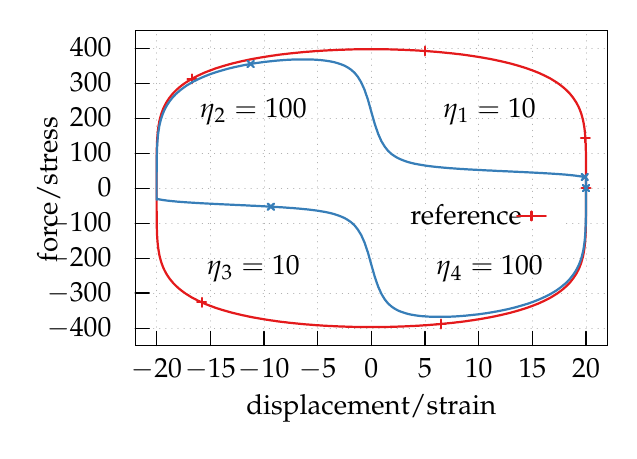
\begin{tikzpicture}[gnuplot]
%% generated with GNUPLOT 5.2p7 (Lua 5.3; terminal rev. Nov 2018, script rev. 107)
%% 08/29/2020 16:55:16
\path (0.000,0.000) rectangle (6.000,4.000);
\gpcolor{color=gp lt color axes}
\gpsetlinetype{gp lt axes}
\gpsetdashtype{gp dt axes}
\gpsetlinewidth{0.50}
\draw[gp path] (0.000,0.222)--(5.999,0.222);
\gpcolor{color=gp lt color border}
\gpsetlinetype{gp lt border}
\gpsetdashtype{gp dt solid}
\gpsetlinewidth{1.00}
\draw[gp path] (0.000,0.222)--(0.180,0.222);
\node[gp node right] at (-0.184,0.222) {$-400$};
\gpcolor{color=gp lt color axes}
\gpsetlinetype{gp lt axes}
\gpsetdashtype{gp dt axes}
\gpsetlinewidth{0.50}
\draw[gp path] (0.000,0.667)--(5.999,0.667);
\gpcolor{color=gp lt color border}
\gpsetlinetype{gp lt border}
\gpsetdashtype{gp dt solid}
\gpsetlinewidth{1.00}
\draw[gp path] (0.000,0.667)--(0.180,0.667);
\node[gp node right] at (-0.184,0.667) {$-300$};
\gpcolor{color=gp lt color axes}
\gpsetlinetype{gp lt axes}
\gpsetdashtype{gp dt axes}
\gpsetlinewidth{0.50}
\draw[gp path] (0.000,1.111)--(5.999,1.111);
\gpcolor{color=gp lt color border}
\gpsetlinetype{gp lt border}
\gpsetdashtype{gp dt solid}
\gpsetlinewidth{1.00}
\draw[gp path] (0.000,1.111)--(0.180,1.111);
\node[gp node right] at (-0.184,1.111) {$-200$};
\gpcolor{color=gp lt color axes}
\gpsetlinetype{gp lt axes}
\gpsetdashtype{gp dt axes}
\gpsetlinewidth{0.50}
\draw[gp path] (0.000,1.555)--(3.379,1.555);
\draw[gp path] (5.399,1.555)--(5.999,1.555);
\gpcolor{color=gp lt color border}
\gpsetlinetype{gp lt border}
\gpsetdashtype{gp dt solid}
\gpsetlinewidth{1.00}
\draw[gp path] (0.000,1.555)--(0.180,1.555);
\node[gp node right] at (-0.184,1.555) {$-100$};
\gpcolor{color=gp lt color axes}
\gpsetlinetype{gp lt axes}
\gpsetdashtype{gp dt axes}
\gpsetlinewidth{0.50}
\draw[gp path] (0.000,2.000)--(5.999,2.000);
\gpcolor{color=gp lt color border}
\gpsetlinetype{gp lt border}
\gpsetdashtype{gp dt solid}
\gpsetlinewidth{1.00}
\draw[gp path] (0.000,2.000)--(0.180,2.000);
\node[gp node right] at (-0.184,2.000) {$0$};
\gpcolor{color=gp lt color axes}
\gpsetlinetype{gp lt axes}
\gpsetdashtype{gp dt axes}
\gpsetlinewidth{0.50}
\draw[gp path] (0.000,2.444)--(5.999,2.444);
\gpcolor{color=gp lt color border}
\gpsetlinetype{gp lt border}
\gpsetdashtype{gp dt solid}
\gpsetlinewidth{1.00}
\draw[gp path] (0.000,2.444)--(0.180,2.444);
\node[gp node right] at (-0.184,2.444) {$100$};
\gpcolor{color=gp lt color axes}
\gpsetlinetype{gp lt axes}
\gpsetdashtype{gp dt axes}
\gpsetlinewidth{0.50}
\draw[gp path] (0.000,2.888)--(5.999,2.888);
\gpcolor{color=gp lt color border}
\gpsetlinetype{gp lt border}
\gpsetdashtype{gp dt solid}
\gpsetlinewidth{1.00}
\draw[gp path] (0.000,2.888)--(0.180,2.888);
\node[gp node right] at (-0.184,2.888) {$200$};
\gpcolor{color=gp lt color axes}
\gpsetlinetype{gp lt axes}
\gpsetdashtype{gp dt axes}
\gpsetlinewidth{0.50}
\draw[gp path] (0.000,3.333)--(5.999,3.333);
\gpcolor{color=gp lt color border}
\gpsetlinetype{gp lt border}
\gpsetdashtype{gp dt solid}
\gpsetlinewidth{1.00}
\draw[gp path] (0.000,3.333)--(0.180,3.333);
\node[gp node right] at (-0.184,3.333) {$300$};
\gpcolor{color=gp lt color axes}
\gpsetlinetype{gp lt axes}
\gpsetdashtype{gp dt axes}
\gpsetlinewidth{0.50}
\draw[gp path] (0.000,3.777)--(5.999,3.777);
\gpcolor{color=gp lt color border}
\gpsetlinetype{gp lt border}
\gpsetdashtype{gp dt solid}
\gpsetlinewidth{1.00}
\draw[gp path] (0.000,3.777)--(0.180,3.777);
\node[gp node right] at (-0.184,3.777) {$400$};
\gpcolor{color=gp lt color axes}
\gpsetlinetype{gp lt axes}
\gpsetdashtype{gp dt axes}
\gpsetlinewidth{0.50}
\draw[gp path] (0.273,0.000)--(0.273,3.999);
\gpcolor{color=gp lt color border}
\gpsetlinetype{gp lt border}
\gpsetdashtype{gp dt solid}
\gpsetlinewidth{1.00}
\draw[gp path] (0.273,0.000)--(0.273,0.180);
\node[gp node center] at (0.273,-0.308) {$-20$};
\gpcolor{color=gp lt color axes}
\gpsetlinetype{gp lt axes}
\gpsetdashtype{gp dt axes}
\gpsetlinewidth{0.50}
\draw[gp path] (0.954,0.000)--(0.954,3.999);
\gpcolor{color=gp lt color border}
\gpsetlinetype{gp lt border}
\gpsetdashtype{gp dt solid}
\gpsetlinewidth{1.00}
\draw[gp path] (0.954,0.000)--(0.954,0.180);
\node[gp node center] at (0.954,-0.308) {$-15$};
\gpcolor{color=gp lt color axes}
\gpsetlinetype{gp lt axes}
\gpsetdashtype{gp dt axes}
\gpsetlinewidth{0.50}
\draw[gp path] (1.636,0.000)--(1.636,3.999);
\gpcolor{color=gp lt color border}
\gpsetlinetype{gp lt border}
\gpsetdashtype{gp dt solid}
\gpsetlinewidth{1.00}
\draw[gp path] (1.636,0.000)--(1.636,0.180);
\node[gp node center] at (1.636,-0.308) {$-10$};
\gpcolor{color=gp lt color axes}
\gpsetlinetype{gp lt axes}
\gpsetdashtype{gp dt axes}
\gpsetlinewidth{0.50}
\draw[gp path] (2.318,0.000)--(2.318,3.999);
\gpcolor{color=gp lt color border}
\gpsetlinetype{gp lt border}
\gpsetdashtype{gp dt solid}
\gpsetlinewidth{1.00}
\draw[gp path] (2.318,0.000)--(2.318,0.180);
\node[gp node center] at (2.318,-0.308) {$-5$};
\gpcolor{color=gp lt color axes}
\gpsetlinetype{gp lt axes}
\gpsetdashtype{gp dt axes}
\gpsetlinewidth{0.50}
\draw[gp path] (3.000,0.000)--(3.000,3.999);
\gpcolor{color=gp lt color border}
\gpsetlinetype{gp lt border}
\gpsetdashtype{gp dt solid}
\gpsetlinewidth{1.00}
\draw[gp path] (3.000,0.000)--(3.000,0.180);
\node[gp node center] at (3.000,-0.308) {$0$};
\gpcolor{color=gp lt color axes}
\gpsetlinetype{gp lt axes}
\gpsetdashtype{gp dt axes}
\gpsetlinewidth{0.50}
\draw[gp path] (3.681,0.000)--(3.681,1.492);
\draw[gp path] (3.681,1.800)--(3.681,3.999);
\gpcolor{color=gp lt color border}
\gpsetlinetype{gp lt border}
\gpsetdashtype{gp dt solid}
\gpsetlinewidth{1.00}
\draw[gp path] (3.681,0.000)--(3.681,0.180);
\node[gp node center] at (3.681,-0.308) {$5$};
\gpcolor{color=gp lt color axes}
\gpsetlinetype{gp lt axes}
\gpsetdashtype{gp dt axes}
\gpsetlinewidth{0.50}
\draw[gp path] (4.363,0.000)--(4.363,1.492);
\draw[gp path] (4.363,1.800)--(4.363,3.999);
\gpcolor{color=gp lt color border}
\gpsetlinetype{gp lt border}
\gpsetdashtype{gp dt solid}
\gpsetlinewidth{1.00}
\draw[gp path] (4.363,0.000)--(4.363,0.180);
\node[gp node center] at (4.363,-0.308) {$10$};
\gpcolor{color=gp lt color axes}
\gpsetlinetype{gp lt axes}
\gpsetdashtype{gp dt axes}
\gpsetlinewidth{0.50}
\draw[gp path] (5.045,0.000)--(5.045,1.492);
\draw[gp path] (5.045,1.800)--(5.045,3.999);
\gpcolor{color=gp lt color border}
\gpsetlinetype{gp lt border}
\gpsetdashtype{gp dt solid}
\gpsetlinewidth{1.00}
\draw[gp path] (5.045,0.000)--(5.045,0.180);
\node[gp node center] at (5.045,-0.308) {$15$};
\gpcolor{color=gp lt color axes}
\gpsetlinetype{gp lt axes}
\gpsetdashtype{gp dt axes}
\gpsetlinewidth{0.50}
\draw[gp path] (5.726,0.000)--(5.726,3.999);
\gpcolor{color=gp lt color border}
\gpsetlinetype{gp lt border}
\gpsetdashtype{gp dt solid}
\gpsetlinewidth{1.00}
\draw[gp path] (5.726,0.000)--(5.726,0.180);
\node[gp node center] at (5.726,-0.308) {$20$};
\draw[gp path] (0.000,3.999)--(0.000,0.000)--(5.999,0.000)--(5.999,3.999)--cycle;
\node[gp node center] at (4.499,2.999) {$\eta_1=10$};
\node[gp node center] at (1.500,2.999) {$\eta_2=100$};
\node[gp node center] at (1.500,1.000) {$\eta_3=10$};
\node[gp node center] at (4.499,1.000) {$\eta_4=100$};
\node[gp node center,rotate=-270] at (-1.074,1.999) {force/stress};
\node[gp node center] at (2.999,-0.769) {displacement/strain};
\gpcolor{rgb color={0.894,0.102,0.110}}
\gpsetlinewidth{2.00}
\draw[gp path] (5.726,2.000)--(5.726,1.730)--(5.725,1.558)--(5.723,1.480)--(5.721,1.416)%
  --(5.718,1.362)--(5.714,1.314)--(5.710,1.271)--(5.705,1.231)--(5.699,1.194)--(5.693,1.159)%
  --(5.686,1.127)--(5.678,1.097)--(5.670,1.068)--(5.661,1.040)--(5.651,1.014)--(5.641,0.988)%
  --(5.630,0.964)--(5.618,0.941)--(5.606,0.918)--(5.593,0.897)--(5.579,0.876)--(5.565,0.855)%
  --(5.550,0.836)--(5.535,0.817)--(5.519,0.798)--(5.502,0.780)--(5.485,0.763)--(5.467,0.746)%
  --(5.448,0.729)--(5.429,0.713)--(5.409,0.697)--(5.389,0.682)--(5.368,0.667)--(5.347,0.653)%
  --(5.324,0.639)--(5.302,0.625)--(5.279,0.611)--(5.255,0.598)--(5.230,0.586)--(5.206,0.573)%
  --(5.180,0.561)--(5.154,0.549)--(5.128,0.537)--(5.101,0.526)--(5.073,0.515)--(5.045,0.504)%
  --(5.016,0.494)--(4.987,0.483)--(4.958,0.473)--(4.928,0.464)--(4.897,0.454)--(4.866,0.445)%
  --(4.835,0.436)--(4.803,0.427)--(4.770,0.418)--(4.738,0.410)--(4.704,0.402)--(4.671,0.394)%
  --(4.637,0.386)--(4.602,0.379)--(4.567,0.371)--(4.532,0.364)--(4.497,0.357)--(4.461,0.351)%
  --(4.424,0.344)--(4.388,0.338)--(4.351,0.332)--(4.313,0.326)--(4.275,0.320)--(4.237,0.315)%
  --(4.199,0.309)--(4.161,0.304)--(4.122,0.299)--(4.082,0.295)--(4.043,0.290)--(4.003,0.286)%
  --(3.963,0.282)--(3.923,0.278)--(3.883,0.274)--(3.842,0.270)--(3.801,0.267)--(3.760,0.264)%
  --(3.719,0.260)--(3.678,0.258)--(3.636,0.255)--(3.594,0.252)--(3.552,0.250)--(3.510,0.248)%
  --(3.468,0.246)--(3.426,0.244)--(3.384,0.242)--(3.341,0.241)--(3.299,0.239)--(3.256,0.238)%
  --(3.213,0.237)--(3.171,0.237)--(3.128,0.236)--(3.085,0.236)--(3.042,0.235)--(2.999,0.235)%
  --(2.957,0.235)--(2.914,0.236)--(2.871,0.236)--(2.828,0.237)--(2.786,0.237)--(2.743,0.238)%
  --(2.700,0.239)--(2.658,0.241)--(2.615,0.242)--(2.573,0.244)--(2.531,0.246)--(2.489,0.248)%
  --(2.447,0.250)--(2.405,0.252)--(2.363,0.255)--(2.321,0.258)--(2.280,0.260)--(2.239,0.264)%
  --(2.198,0.267)--(2.157,0.270)--(2.116,0.274)--(2.076,0.278)--(2.036,0.282)--(1.996,0.286)%
  --(1.956,0.290)--(1.917,0.295)--(1.877,0.299)--(1.838,0.304)--(1.800,0.309)--(1.762,0.315)%
  --(1.724,0.320)--(1.686,0.326)--(1.648,0.332)--(1.611,0.338)--(1.575,0.344)--(1.538,0.351)%
  --(1.502,0.357)--(1.467,0.364)--(1.432,0.371)--(1.397,0.379)--(1.362,0.386)--(1.328,0.394)%
  --(1.295,0.402)--(1.261,0.410)--(1.229,0.418)--(1.196,0.427)--(1.164,0.436)--(1.133,0.445)%
  --(1.102,0.454)--(1.071,0.464)--(1.041,0.473)--(1.012,0.483)--(0.983,0.494)--(0.954,0.504)%
  --(0.926,0.515)--(0.898,0.526)--(0.871,0.537)--(0.845,0.549)--(0.819,0.561)--(0.793,0.573)%
  --(0.769,0.586)--(0.744,0.598)--(0.720,0.611)--(0.697,0.625)--(0.675,0.639)--(0.652,0.653)%
  --(0.631,0.667)--(0.610,0.682)--(0.590,0.697)--(0.570,0.713)--(0.551,0.729)--(0.532,0.746)%
  --(0.514,0.763)--(0.497,0.780)--(0.480,0.798)--(0.464,0.817)--(0.449,0.836)--(0.434,0.855)%
  --(0.420,0.876)--(0.406,0.897)--(0.393,0.918)--(0.381,0.941)--(0.369,0.964)--(0.358,0.988)%
  --(0.348,1.014)--(0.338,1.040)--(0.329,1.068)--(0.321,1.097)--(0.313,1.127)--(0.306,1.159)%
  --(0.300,1.194)--(0.294,1.231)--(0.289,1.271)--(0.285,1.314)--(0.281,1.362)--(0.278,1.416)%
  --(0.276,1.480)--(0.274,1.558)--(0.273,1.730)--(0.273,1.999)--(0.273,2.269)--(0.274,2.441)%
  --(0.276,2.519)--(0.278,2.583)--(0.281,2.637)--(0.285,2.685)--(0.289,2.728)--(0.294,2.768)%
  --(0.300,2.805)--(0.306,2.840)--(0.313,2.872)--(0.321,2.902)--(0.329,2.931)--(0.338,2.959)%
  --(0.348,2.985)--(0.358,3.011)--(0.369,3.035)--(0.381,3.058)--(0.393,3.081)--(0.406,3.102)%
  --(0.420,3.123)--(0.434,3.144)--(0.449,3.163)--(0.464,3.182)--(0.480,3.201)--(0.497,3.219)%
  --(0.514,3.236)--(0.532,3.253)--(0.551,3.270)--(0.570,3.286)--(0.590,3.302)--(0.610,3.317)%
  --(0.631,3.332)--(0.652,3.346)--(0.675,3.360)--(0.697,3.374)--(0.720,3.388)--(0.744,3.401)%
  --(0.769,3.413)--(0.793,3.426)--(0.819,3.438)--(0.845,3.450)--(0.871,3.462)--(0.898,3.473)%
  --(0.926,3.484)--(0.954,3.495)--(0.983,3.505)--(1.012,3.516)--(1.041,3.526)--(1.071,3.535)%
  --(1.102,3.545)--(1.133,3.554)--(1.164,3.563)--(1.196,3.572)--(1.229,3.581)--(1.261,3.589)%
  --(1.295,3.597)--(1.328,3.605)--(1.362,3.613)--(1.397,3.620)--(1.432,3.628)--(1.467,3.635)%
  --(1.502,3.642)--(1.538,3.648)--(1.575,3.655)--(1.611,3.661)--(1.648,3.667)--(1.686,3.673)%
  --(1.724,3.679)--(1.762,3.684)--(1.800,3.690)--(1.838,3.695)--(1.877,3.700)--(1.917,3.704)%
  --(1.956,3.709)--(1.996,3.713)--(2.036,3.717)--(2.076,3.721)--(2.116,3.725)--(2.157,3.729)%
  --(2.198,3.732)--(2.239,3.735)--(2.280,3.739)--(2.321,3.741)--(2.363,3.744)--(2.405,3.747)%
  --(2.447,3.749)--(2.489,3.751)--(2.531,3.753)--(2.573,3.755)--(2.615,3.757)--(2.658,3.758)%
  --(2.700,3.760)--(2.743,3.761)--(2.786,3.762)--(2.828,3.762)--(2.871,3.763)--(2.914,3.763)%
  --(2.957,3.764)--(2.999,3.764)--(3.042,3.764)--(3.085,3.763)--(3.128,3.763)--(3.171,3.762)%
  --(3.213,3.762)--(3.256,3.761)--(3.299,3.760)--(3.341,3.758)--(3.384,3.757)--(3.426,3.755)%
  --(3.468,3.753)--(3.510,3.751)--(3.552,3.749)--(3.594,3.747)--(3.636,3.744)--(3.678,3.741)%
  --(3.719,3.739)--(3.760,3.735)--(3.801,3.732)--(3.842,3.729)--(3.883,3.725)--(3.923,3.721)%
  --(3.963,3.717)--(4.003,3.713)--(4.043,3.709)--(4.082,3.704)--(4.122,3.700)--(4.161,3.695)%
  --(4.199,3.690)--(4.237,3.684)--(4.275,3.679)--(4.313,3.673)--(4.351,3.667)--(4.388,3.661)%
  --(4.424,3.655)--(4.461,3.648)--(4.497,3.642)--(4.532,3.635)--(4.567,3.628)--(4.602,3.620)%
  --(4.637,3.613)--(4.671,3.605)--(4.704,3.597)--(4.738,3.589)--(4.770,3.581)--(4.803,3.572)%
  --(4.835,3.563)--(4.866,3.554)--(4.897,3.545)--(4.928,3.535)--(4.958,3.526)--(4.987,3.516)%
  --(5.016,3.505)--(5.045,3.495)--(5.073,3.484)--(5.101,3.473)--(5.128,3.462)--(5.154,3.450)%
  --(5.180,3.438)--(5.206,3.426)--(5.230,3.413)--(5.255,3.401)--(5.279,3.388)--(5.302,3.374)%
  --(5.324,3.360)--(5.347,3.346)--(5.368,3.332)--(5.389,3.317)--(5.409,3.302)--(5.429,3.286)%
  --(5.448,3.270)--(5.467,3.253)--(5.485,3.236)--(5.502,3.219)--(5.519,3.201)--(5.535,3.182)%
  --(5.550,3.163)--(5.565,3.144)--(5.579,3.123)--(5.593,3.102)--(5.606,3.081)--(5.618,3.058)%
  --(5.630,3.035)--(5.641,3.011)--(5.651,2.985)--(5.661,2.959)--(5.670,2.931)--(5.678,2.902)%
  --(5.686,2.872)--(5.693,2.840)--(5.699,2.805)--(5.705,2.768)--(5.710,2.728)--(5.714,2.685)%
  --(5.718,2.637)--(5.721,2.583)--(5.723,2.519)--(5.725,2.441)--(5.726,2.269)--(5.726,1.999);
\gpsetpointsize{4.00}
\gppoint{gp mark 1}{(5.726,2.000)}
\gppoint{gp mark 1}{(3.883,0.274)}
\gppoint{gp mark 1}{(0.845,0.549)}
\gppoint{gp mark 1}{(0.720,3.388)}
\gppoint{gp mark 1}{(3.678,3.741)}
\gppoint{gp mark 1}{(5.718,2.637)}
\gpcolor{rgb color={0.216,0.494,0.722}}
\draw[gp path] (5.726,2.000)--(5.726,1.817)--(5.725,1.661)--(5.723,1.573)--(5.721,1.501)%
  --(5.718,1.439)--(5.714,1.386)--(5.710,1.338)--(5.705,1.295)--(5.699,1.255)--(5.693,1.218)%
  --(5.686,1.184)--(5.678,1.152)--(5.670,1.121)--(5.661,1.093)--(5.651,1.065)--(5.641,1.039)%
  --(5.630,1.014)--(5.618,0.990)--(5.606,0.967)--(5.593,0.944)--(5.579,0.923)--(5.565,0.902)%
  --(5.550,0.882)--(5.535,0.863)--(5.519,0.844)--(5.502,0.826)--(5.485,0.808)--(5.467,0.791)%
  --(5.448,0.775)--(5.429,0.759)--(5.409,0.743)--(5.389,0.728)--(5.368,0.713)--(5.347,0.698)%
  --(5.324,0.684)--(5.302,0.671)--(5.279,0.657)--(5.255,0.644)--(5.230,0.632)--(5.206,0.620)%
  --(5.180,0.608)--(5.154,0.596)--(5.128,0.585)--(5.101,0.574)--(5.073,0.563)--(5.045,0.552)%
  --(5.016,0.542)--(4.987,0.532)--(4.958,0.523)--(4.928,0.514)--(4.897,0.505)--(4.866,0.496)%
  --(4.835,0.487)--(4.803,0.479)--(4.770,0.471)--(4.738,0.463)--(4.704,0.456)--(4.671,0.449)%
  --(4.637,0.442)--(4.602,0.435)--(4.567,0.429)--(4.532,0.423)--(4.497,0.417)--(4.461,0.411)%
  --(4.424,0.406)--(4.388,0.401)--(4.351,0.396)--(4.313,0.392)--(4.275,0.388)--(4.237,0.384)%
  --(4.199,0.380)--(4.161,0.377)--(4.122,0.374)--(4.082,0.371)--(4.043,0.369)--(4.003,0.367)%
  --(3.963,0.366)--(3.923,0.365)--(3.883,0.365)--(3.842,0.365)--(3.801,0.365)--(3.760,0.366)%
  --(3.719,0.368)--(3.678,0.371)--(3.636,0.374)--(3.594,0.379)--(3.552,0.385)--(3.510,0.392)%
  --(3.468,0.401)--(3.426,0.413)--(3.384,0.427)--(3.341,0.444)--(3.299,0.467)--(3.256,0.496)%
  --(3.213,0.534)--(3.171,0.585)--(3.128,0.656)--(3.085,0.752)--(3.042,0.878)--(2.999,1.029)%
  --(2.957,1.180)--(2.914,1.307)--(2.871,1.404)--(2.828,1.474)--(2.786,1.527)--(2.743,1.566)%
  --(2.700,1.596)--(2.658,1.620)--(2.615,1.639)--(2.573,1.655)--(2.531,1.669)--(2.489,1.680)%
  --(2.447,1.690)--(2.405,1.698)--(2.363,1.705)--(2.321,1.712)--(2.280,1.718)--(2.239,1.723)%
  --(2.198,1.728)--(2.157,1.732)--(2.116,1.736)--(2.076,1.740)--(2.036,1.743)--(1.996,1.747)%
  --(1.956,1.749)--(1.917,1.752)--(1.877,1.755)--(1.838,1.757)--(1.800,1.760)--(1.762,1.762)%
  --(1.724,1.764)--(1.686,1.766)--(1.648,1.768)--(1.611,1.770)--(1.575,1.772)--(1.538,1.774)%
  --(1.502,1.776)--(1.467,1.777)--(1.432,1.779)--(1.397,1.781)--(1.362,1.782)--(1.328,1.784)%
  --(1.295,1.785)--(1.261,1.787)--(1.229,1.789)--(1.196,1.790)--(1.164,1.792)--(1.133,1.793)%
  --(1.102,1.794)--(1.071,1.796)--(1.041,1.797)--(1.012,1.799)--(0.983,1.800)--(0.954,1.802)%
  --(0.926,1.803)--(0.898,1.805)--(0.871,1.806)--(0.845,1.807)--(0.819,1.809)--(0.793,1.810)%
  --(0.769,1.812)--(0.744,1.813)--(0.720,1.815)--(0.697,1.816)--(0.675,1.818)--(0.652,1.819)%
  --(0.631,1.821)--(0.610,1.822)--(0.590,1.824)--(0.570,1.825)--(0.551,1.827)--(0.532,1.828)%
  --(0.514,1.830)--(0.497,1.832)--(0.480,1.833)--(0.464,1.835)--(0.449,1.836)--(0.434,1.838)%
  --(0.420,1.840)--(0.406,1.841)--(0.393,1.843)--(0.381,1.845)--(0.369,1.846)--(0.358,1.848)%
  --(0.348,1.849)--(0.338,1.851)--(0.329,1.852)--(0.321,1.854)--(0.313,1.855)--(0.306,1.857)%
  --(0.300,1.858)--(0.294,1.859)--(0.289,1.859)--(0.285,1.859)--(0.281,1.858)--(0.278,1.857)%
  --(0.276,1.854)--(0.274,1.852)--(0.273,1.886)--(0.273,1.999)--(0.273,2.182)--(0.274,2.338)%
  --(0.276,2.426)--(0.278,2.498)--(0.281,2.560)--(0.285,2.613)--(0.289,2.661)--(0.294,2.704)%
  --(0.300,2.744)--(0.306,2.781)--(0.313,2.815)--(0.321,2.847)--(0.329,2.878)--(0.338,2.906)%
  --(0.348,2.934)--(0.358,2.960)--(0.369,2.985)--(0.381,3.009)--(0.393,3.032)--(0.406,3.055)%
  --(0.420,3.076)--(0.434,3.097)--(0.449,3.117)--(0.464,3.136)--(0.480,3.155)--(0.497,3.173)%
  --(0.514,3.191)--(0.532,3.208)--(0.551,3.224)--(0.570,3.240)--(0.590,3.256)--(0.610,3.271)%
  --(0.631,3.286)--(0.652,3.301)--(0.675,3.315)--(0.697,3.328)--(0.720,3.342)--(0.744,3.355)%
  --(0.769,3.367)--(0.793,3.379)--(0.819,3.391)--(0.845,3.403)--(0.871,3.414)--(0.898,3.425)%
  --(0.926,3.436)--(0.954,3.447)--(0.983,3.457)--(1.012,3.467)--(1.041,3.476)--(1.071,3.485)%
  --(1.102,3.494)--(1.133,3.503)--(1.164,3.512)--(1.196,3.520)--(1.229,3.528)--(1.261,3.536)%
  --(1.295,3.543)--(1.328,3.550)--(1.362,3.557)--(1.397,3.564)--(1.432,3.570)--(1.467,3.576)%
  --(1.502,3.582)--(1.538,3.588)--(1.575,3.593)--(1.611,3.598)--(1.648,3.603)--(1.686,3.607)%
  --(1.724,3.611)--(1.762,3.615)--(1.800,3.619)--(1.838,3.622)--(1.877,3.625)--(1.917,3.628)%
  --(1.956,3.630)--(1.996,3.632)--(2.036,3.633)--(2.076,3.634)--(2.116,3.634)--(2.157,3.634)%
  --(2.198,3.634)--(2.239,3.633)--(2.280,3.631)--(2.321,3.628)--(2.363,3.625)--(2.405,3.620)%
  --(2.447,3.614)--(2.489,3.607)--(2.531,3.598)--(2.573,3.586)--(2.615,3.572)--(2.658,3.555)%
  --(2.700,3.532)--(2.743,3.503)--(2.786,3.465)--(2.828,3.414)--(2.871,3.343)--(2.914,3.247)%
  --(2.957,3.121)--(2.999,2.970)--(3.042,2.819)--(3.085,2.692)--(3.128,2.595)--(3.171,2.525)%
  --(3.213,2.472)--(3.256,2.433)--(3.299,2.403)--(3.341,2.379)--(3.384,2.360)--(3.426,2.344)%
  --(3.468,2.330)--(3.510,2.319)--(3.552,2.309)--(3.594,2.301)--(3.636,2.294)--(3.678,2.287)%
  --(3.719,2.281)--(3.760,2.276)--(3.801,2.271)--(3.842,2.267)--(3.883,2.263)--(3.923,2.259)%
  --(3.963,2.256)--(4.003,2.252)--(4.043,2.250)--(4.082,2.247)--(4.122,2.244)--(4.161,2.242)%
  --(4.199,2.239)--(4.237,2.237)--(4.275,2.235)--(4.313,2.233)--(4.351,2.231)--(4.388,2.229)%
  --(4.424,2.227)--(4.461,2.225)--(4.497,2.223)--(4.532,2.222)--(4.567,2.220)--(4.602,2.218)%
  --(4.637,2.217)--(4.671,2.215)--(4.704,2.214)--(4.738,2.212)--(4.770,2.210)--(4.803,2.209)%
  --(4.835,2.207)--(4.866,2.206)--(4.897,2.205)--(4.928,2.203)--(4.958,2.202)--(4.987,2.200)%
  --(5.016,2.199)--(5.045,2.197)--(5.073,2.196)--(5.101,2.194)--(5.128,2.193)--(5.154,2.192)%
  --(5.180,2.190)--(5.206,2.189)--(5.230,2.187)--(5.255,2.186)--(5.279,2.184)--(5.302,2.183)%
  --(5.324,2.181)--(5.347,2.180)--(5.368,2.178)--(5.389,2.177)--(5.409,2.175)--(5.429,2.174)%
  --(5.448,2.172)--(5.467,2.171)--(5.485,2.169)--(5.502,2.167)--(5.519,2.166)--(5.535,2.164)%
  --(5.550,2.163)--(5.565,2.161)--(5.579,2.159)--(5.593,2.158)--(5.606,2.156)--(5.618,2.154)%
  --(5.630,2.153)--(5.641,2.151)--(5.651,2.150)--(5.661,2.148)--(5.670,2.147)--(5.678,2.145)%
  --(5.686,2.144)--(5.693,2.142)--(5.699,2.141)--(5.705,2.140)--(5.710,2.140)--(5.714,2.140)%
  --(5.718,2.141)--(5.721,2.142)--(5.723,2.145)--(5.725,2.147)--(5.726,2.113)--(5.726,1.999);
\gppoint{gp mark 2}{(5.726,2.000)}
\gppoint{gp mark 2}{(1.724,1.764)}
\gppoint{gp mark 2}{(1.467,3.576)}
\gppoint{gp mark 2}{(5.710,2.140)}
\gpfill{color=gpbgfillcolor} (3.379,1.492)--(5.399,1.492)--(5.399,1.800)--(3.379,1.800)--cycle;
\gpcolor{color=gp lt color border}
\node[gp node left] at (3.379,1.646) {reference};
\gpcolor{rgb color={0.894,0.102,0.110}}
\draw[gp path] (4.851,1.646)--(5.215,1.646);
\gppoint{gp mark 1}{(5.033,1.646)}
\gpcolor{color=gp lt color border}
\gpsetlinewidth{1.00}
\draw[gp path] (0.000,3.999)--(0.000,0.000)--(5.999,0.000)--(5.999,3.999)--cycle;
%% coordinates of the plot area
\gpdefrectangularnode{gp plot 1}{\pgfpoint{0.000cm}{0.000cm}}{\pgfpoint{5.999cm}{3.999cm}}
\end{tikzpicture}
%% gnuplot variables

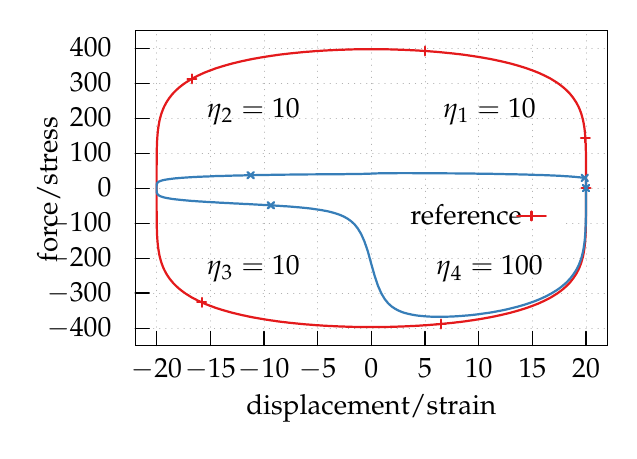
\begin{tikzpicture}[gnuplot]
%% generated with GNUPLOT 5.2p7 (Lua 5.3; terminal rev. Nov 2018, script rev. 107)
%% 08/29/2020 16:55:16
\path (0.000,0.000) rectangle (6.000,4.000);
\gpcolor{color=gp lt color axes}
\gpsetlinetype{gp lt axes}
\gpsetdashtype{gp dt axes}
\gpsetlinewidth{0.50}
\draw[gp path] (0.000,0.222)--(5.999,0.222);
\gpcolor{color=gp lt color border}
\gpsetlinetype{gp lt border}
\gpsetdashtype{gp dt solid}
\gpsetlinewidth{1.00}
\draw[gp path] (0.000,0.222)--(0.180,0.222);
\node[gp node right] at (-0.184,0.222) {$-400$};
\gpcolor{color=gp lt color axes}
\gpsetlinetype{gp lt axes}
\gpsetdashtype{gp dt axes}
\gpsetlinewidth{0.50}
\draw[gp path] (0.000,0.667)--(5.999,0.667);
\gpcolor{color=gp lt color border}
\gpsetlinetype{gp lt border}
\gpsetdashtype{gp dt solid}
\gpsetlinewidth{1.00}
\draw[gp path] (0.000,0.667)--(0.180,0.667);
\node[gp node right] at (-0.184,0.667) {$-300$};
\gpcolor{color=gp lt color axes}
\gpsetlinetype{gp lt axes}
\gpsetdashtype{gp dt axes}
\gpsetlinewidth{0.50}
\draw[gp path] (0.000,1.111)--(5.999,1.111);
\gpcolor{color=gp lt color border}
\gpsetlinetype{gp lt border}
\gpsetdashtype{gp dt solid}
\gpsetlinewidth{1.00}
\draw[gp path] (0.000,1.111)--(0.180,1.111);
\node[gp node right] at (-0.184,1.111) {$-200$};
\gpcolor{color=gp lt color axes}
\gpsetlinetype{gp lt axes}
\gpsetdashtype{gp dt axes}
\gpsetlinewidth{0.50}
\draw[gp path] (0.000,1.555)--(3.379,1.555);
\draw[gp path] (5.399,1.555)--(5.999,1.555);
\gpcolor{color=gp lt color border}
\gpsetlinetype{gp lt border}
\gpsetdashtype{gp dt solid}
\gpsetlinewidth{1.00}
\draw[gp path] (0.000,1.555)--(0.180,1.555);
\node[gp node right] at (-0.184,1.555) {$-100$};
\gpcolor{color=gp lt color axes}
\gpsetlinetype{gp lt axes}
\gpsetdashtype{gp dt axes}
\gpsetlinewidth{0.50}
\draw[gp path] (0.000,2.000)--(5.999,2.000);
\gpcolor{color=gp lt color border}
\gpsetlinetype{gp lt border}
\gpsetdashtype{gp dt solid}
\gpsetlinewidth{1.00}
\draw[gp path] (0.000,2.000)--(0.180,2.000);
\node[gp node right] at (-0.184,2.000) {$0$};
\gpcolor{color=gp lt color axes}
\gpsetlinetype{gp lt axes}
\gpsetdashtype{gp dt axes}
\gpsetlinewidth{0.50}
\draw[gp path] (0.000,2.444)--(5.999,2.444);
\gpcolor{color=gp lt color border}
\gpsetlinetype{gp lt border}
\gpsetdashtype{gp dt solid}
\gpsetlinewidth{1.00}
\draw[gp path] (0.000,2.444)--(0.180,2.444);
\node[gp node right] at (-0.184,2.444) {$100$};
\gpcolor{color=gp lt color axes}
\gpsetlinetype{gp lt axes}
\gpsetdashtype{gp dt axes}
\gpsetlinewidth{0.50}
\draw[gp path] (0.000,2.888)--(5.999,2.888);
\gpcolor{color=gp lt color border}
\gpsetlinetype{gp lt border}
\gpsetdashtype{gp dt solid}
\gpsetlinewidth{1.00}
\draw[gp path] (0.000,2.888)--(0.180,2.888);
\node[gp node right] at (-0.184,2.888) {$200$};
\gpcolor{color=gp lt color axes}
\gpsetlinetype{gp lt axes}
\gpsetdashtype{gp dt axes}
\gpsetlinewidth{0.50}
\draw[gp path] (0.000,3.333)--(5.999,3.333);
\gpcolor{color=gp lt color border}
\gpsetlinetype{gp lt border}
\gpsetdashtype{gp dt solid}
\gpsetlinewidth{1.00}
\draw[gp path] (0.000,3.333)--(0.180,3.333);
\node[gp node right] at (-0.184,3.333) {$300$};
\gpcolor{color=gp lt color axes}
\gpsetlinetype{gp lt axes}
\gpsetdashtype{gp dt axes}
\gpsetlinewidth{0.50}
\draw[gp path] (0.000,3.777)--(5.999,3.777);
\gpcolor{color=gp lt color border}
\gpsetlinetype{gp lt border}
\gpsetdashtype{gp dt solid}
\gpsetlinewidth{1.00}
\draw[gp path] (0.000,3.777)--(0.180,3.777);
\node[gp node right] at (-0.184,3.777) {$400$};
\gpcolor{color=gp lt color axes}
\gpsetlinetype{gp lt axes}
\gpsetdashtype{gp dt axes}
\gpsetlinewidth{0.50}
\draw[gp path] (0.273,0.000)--(0.273,3.999);
\gpcolor{color=gp lt color border}
\gpsetlinetype{gp lt border}
\gpsetdashtype{gp dt solid}
\gpsetlinewidth{1.00}
\draw[gp path] (0.273,0.000)--(0.273,0.180);
\node[gp node center] at (0.273,-0.308) {$-20$};
\gpcolor{color=gp lt color axes}
\gpsetlinetype{gp lt axes}
\gpsetdashtype{gp dt axes}
\gpsetlinewidth{0.50}
\draw[gp path] (0.954,0.000)--(0.954,3.999);
\gpcolor{color=gp lt color border}
\gpsetlinetype{gp lt border}
\gpsetdashtype{gp dt solid}
\gpsetlinewidth{1.00}
\draw[gp path] (0.954,0.000)--(0.954,0.180);
\node[gp node center] at (0.954,-0.308) {$-15$};
\gpcolor{color=gp lt color axes}
\gpsetlinetype{gp lt axes}
\gpsetdashtype{gp dt axes}
\gpsetlinewidth{0.50}
\draw[gp path] (1.636,0.000)--(1.636,3.999);
\gpcolor{color=gp lt color border}
\gpsetlinetype{gp lt border}
\gpsetdashtype{gp dt solid}
\gpsetlinewidth{1.00}
\draw[gp path] (1.636,0.000)--(1.636,0.180);
\node[gp node center] at (1.636,-0.308) {$-10$};
\gpcolor{color=gp lt color axes}
\gpsetlinetype{gp lt axes}
\gpsetdashtype{gp dt axes}
\gpsetlinewidth{0.50}
\draw[gp path] (2.318,0.000)--(2.318,3.999);
\gpcolor{color=gp lt color border}
\gpsetlinetype{gp lt border}
\gpsetdashtype{gp dt solid}
\gpsetlinewidth{1.00}
\draw[gp path] (2.318,0.000)--(2.318,0.180);
\node[gp node center] at (2.318,-0.308) {$-5$};
\gpcolor{color=gp lt color axes}
\gpsetlinetype{gp lt axes}
\gpsetdashtype{gp dt axes}
\gpsetlinewidth{0.50}
\draw[gp path] (3.000,0.000)--(3.000,3.999);
\gpcolor{color=gp lt color border}
\gpsetlinetype{gp lt border}
\gpsetdashtype{gp dt solid}
\gpsetlinewidth{1.00}
\draw[gp path] (3.000,0.000)--(3.000,0.180);
\node[gp node center] at (3.000,-0.308) {$0$};
\gpcolor{color=gp lt color axes}
\gpsetlinetype{gp lt axes}
\gpsetdashtype{gp dt axes}
\gpsetlinewidth{0.50}
\draw[gp path] (3.681,0.000)--(3.681,1.492);
\draw[gp path] (3.681,1.800)--(3.681,3.999);
\gpcolor{color=gp lt color border}
\gpsetlinetype{gp lt border}
\gpsetdashtype{gp dt solid}
\gpsetlinewidth{1.00}
\draw[gp path] (3.681,0.000)--(3.681,0.180);
\node[gp node center] at (3.681,-0.308) {$5$};
\gpcolor{color=gp lt color axes}
\gpsetlinetype{gp lt axes}
\gpsetdashtype{gp dt axes}
\gpsetlinewidth{0.50}
\draw[gp path] (4.363,0.000)--(4.363,1.492);
\draw[gp path] (4.363,1.800)--(4.363,3.999);
\gpcolor{color=gp lt color border}
\gpsetlinetype{gp lt border}
\gpsetdashtype{gp dt solid}
\gpsetlinewidth{1.00}
\draw[gp path] (4.363,0.000)--(4.363,0.180);
\node[gp node center] at (4.363,-0.308) {$10$};
\gpcolor{color=gp lt color axes}
\gpsetlinetype{gp lt axes}
\gpsetdashtype{gp dt axes}
\gpsetlinewidth{0.50}
\draw[gp path] (5.045,0.000)--(5.045,1.492);
\draw[gp path] (5.045,1.800)--(5.045,3.999);
\gpcolor{color=gp lt color border}
\gpsetlinetype{gp lt border}
\gpsetdashtype{gp dt solid}
\gpsetlinewidth{1.00}
\draw[gp path] (5.045,0.000)--(5.045,0.180);
\node[gp node center] at (5.045,-0.308) {$15$};
\gpcolor{color=gp lt color axes}
\gpsetlinetype{gp lt axes}
\gpsetdashtype{gp dt axes}
\gpsetlinewidth{0.50}
\draw[gp path] (5.726,0.000)--(5.726,3.999);
\gpcolor{color=gp lt color border}
\gpsetlinetype{gp lt border}
\gpsetdashtype{gp dt solid}
\gpsetlinewidth{1.00}
\draw[gp path] (5.726,0.000)--(5.726,0.180);
\node[gp node center] at (5.726,-0.308) {$20$};
\draw[gp path] (0.000,3.999)--(0.000,0.000)--(5.999,0.000)--(5.999,3.999)--cycle;
\node[gp node center] at (4.499,2.999) {$\eta_1=10$};
\node[gp node center] at (1.500,2.999) {$\eta_2=10$};
\node[gp node center] at (1.500,1.000) {$\eta_3=10$};
\node[gp node center] at (4.499,1.000) {$\eta_4=100$};
\node[gp node center,rotate=-270] at (-1.074,1.999) {force/stress};
\node[gp node center] at (2.999,-0.769) {displacement/strain};
\gpcolor{rgb color={0.894,0.102,0.110}}
\gpsetlinewidth{2.00}
\draw[gp path] (5.726,2.000)--(5.726,1.730)--(5.725,1.558)--(5.723,1.480)--(5.721,1.416)%
  --(5.718,1.362)--(5.714,1.314)--(5.710,1.271)--(5.705,1.231)--(5.699,1.194)--(5.693,1.159)%
  --(5.686,1.127)--(5.678,1.097)--(5.670,1.068)--(5.661,1.040)--(5.651,1.014)--(5.641,0.988)%
  --(5.630,0.964)--(5.618,0.941)--(5.606,0.918)--(5.593,0.897)--(5.579,0.876)--(5.565,0.855)%
  --(5.550,0.836)--(5.535,0.817)--(5.519,0.798)--(5.502,0.780)--(5.485,0.763)--(5.467,0.746)%
  --(5.448,0.729)--(5.429,0.713)--(5.409,0.697)--(5.389,0.682)--(5.368,0.667)--(5.347,0.653)%
  --(5.324,0.639)--(5.302,0.625)--(5.279,0.611)--(5.255,0.598)--(5.230,0.586)--(5.206,0.573)%
  --(5.180,0.561)--(5.154,0.549)--(5.128,0.537)--(5.101,0.526)--(5.073,0.515)--(5.045,0.504)%
  --(5.016,0.494)--(4.987,0.483)--(4.958,0.473)--(4.928,0.464)--(4.897,0.454)--(4.866,0.445)%
  --(4.835,0.436)--(4.803,0.427)--(4.770,0.418)--(4.738,0.410)--(4.704,0.402)--(4.671,0.394)%
  --(4.637,0.386)--(4.602,0.379)--(4.567,0.371)--(4.532,0.364)--(4.497,0.357)--(4.461,0.351)%
  --(4.424,0.344)--(4.388,0.338)--(4.351,0.332)--(4.313,0.326)--(4.275,0.320)--(4.237,0.315)%
  --(4.199,0.309)--(4.161,0.304)--(4.122,0.299)--(4.082,0.295)--(4.043,0.290)--(4.003,0.286)%
  --(3.963,0.282)--(3.923,0.278)--(3.883,0.274)--(3.842,0.270)--(3.801,0.267)--(3.760,0.264)%
  --(3.719,0.260)--(3.678,0.258)--(3.636,0.255)--(3.594,0.252)--(3.552,0.250)--(3.510,0.248)%
  --(3.468,0.246)--(3.426,0.244)--(3.384,0.242)--(3.341,0.241)--(3.299,0.239)--(3.256,0.238)%
  --(3.213,0.237)--(3.171,0.237)--(3.128,0.236)--(3.085,0.236)--(3.042,0.235)--(2.999,0.235)%
  --(2.957,0.235)--(2.914,0.236)--(2.871,0.236)--(2.828,0.237)--(2.786,0.237)--(2.743,0.238)%
  --(2.700,0.239)--(2.658,0.241)--(2.615,0.242)--(2.573,0.244)--(2.531,0.246)--(2.489,0.248)%
  --(2.447,0.250)--(2.405,0.252)--(2.363,0.255)--(2.321,0.258)--(2.280,0.260)--(2.239,0.264)%
  --(2.198,0.267)--(2.157,0.270)--(2.116,0.274)--(2.076,0.278)--(2.036,0.282)--(1.996,0.286)%
  --(1.956,0.290)--(1.917,0.295)--(1.877,0.299)--(1.838,0.304)--(1.800,0.309)--(1.762,0.315)%
  --(1.724,0.320)--(1.686,0.326)--(1.648,0.332)--(1.611,0.338)--(1.575,0.344)--(1.538,0.351)%
  --(1.502,0.357)--(1.467,0.364)--(1.432,0.371)--(1.397,0.379)--(1.362,0.386)--(1.328,0.394)%
  --(1.295,0.402)--(1.261,0.410)--(1.229,0.418)--(1.196,0.427)--(1.164,0.436)--(1.133,0.445)%
  --(1.102,0.454)--(1.071,0.464)--(1.041,0.473)--(1.012,0.483)--(0.983,0.494)--(0.954,0.504)%
  --(0.926,0.515)--(0.898,0.526)--(0.871,0.537)--(0.845,0.549)--(0.819,0.561)--(0.793,0.573)%
  --(0.769,0.586)--(0.744,0.598)--(0.720,0.611)--(0.697,0.625)--(0.675,0.639)--(0.652,0.653)%
  --(0.631,0.667)--(0.610,0.682)--(0.590,0.697)--(0.570,0.713)--(0.551,0.729)--(0.532,0.746)%
  --(0.514,0.763)--(0.497,0.780)--(0.480,0.798)--(0.464,0.817)--(0.449,0.836)--(0.434,0.855)%
  --(0.420,0.876)--(0.406,0.897)--(0.393,0.918)--(0.381,0.941)--(0.369,0.964)--(0.358,0.988)%
  --(0.348,1.014)--(0.338,1.040)--(0.329,1.068)--(0.321,1.097)--(0.313,1.127)--(0.306,1.159)%
  --(0.300,1.194)--(0.294,1.231)--(0.289,1.271)--(0.285,1.314)--(0.281,1.362)--(0.278,1.416)%
  --(0.276,1.480)--(0.274,1.558)--(0.273,1.730)--(0.273,1.999)--(0.273,2.269)--(0.274,2.441)%
  --(0.276,2.519)--(0.278,2.583)--(0.281,2.637)--(0.285,2.685)--(0.289,2.728)--(0.294,2.768)%
  --(0.300,2.805)--(0.306,2.840)--(0.313,2.872)--(0.321,2.902)--(0.329,2.931)--(0.338,2.959)%
  --(0.348,2.985)--(0.358,3.011)--(0.369,3.035)--(0.381,3.058)--(0.393,3.081)--(0.406,3.102)%
  --(0.420,3.123)--(0.434,3.144)--(0.449,3.163)--(0.464,3.182)--(0.480,3.201)--(0.497,3.219)%
  --(0.514,3.236)--(0.532,3.253)--(0.551,3.270)--(0.570,3.286)--(0.590,3.302)--(0.610,3.317)%
  --(0.631,3.332)--(0.652,3.346)--(0.675,3.360)--(0.697,3.374)--(0.720,3.388)--(0.744,3.401)%
  --(0.769,3.413)--(0.793,3.426)--(0.819,3.438)--(0.845,3.450)--(0.871,3.462)--(0.898,3.473)%
  --(0.926,3.484)--(0.954,3.495)--(0.983,3.505)--(1.012,3.516)--(1.041,3.526)--(1.071,3.535)%
  --(1.102,3.545)--(1.133,3.554)--(1.164,3.563)--(1.196,3.572)--(1.229,3.581)--(1.261,3.589)%
  --(1.295,3.597)--(1.328,3.605)--(1.362,3.613)--(1.397,3.620)--(1.432,3.628)--(1.467,3.635)%
  --(1.502,3.642)--(1.538,3.648)--(1.575,3.655)--(1.611,3.661)--(1.648,3.667)--(1.686,3.673)%
  --(1.724,3.679)--(1.762,3.684)--(1.800,3.690)--(1.838,3.695)--(1.877,3.700)--(1.917,3.704)%
  --(1.956,3.709)--(1.996,3.713)--(2.036,3.717)--(2.076,3.721)--(2.116,3.725)--(2.157,3.729)%
  --(2.198,3.732)--(2.239,3.735)--(2.280,3.739)--(2.321,3.741)--(2.363,3.744)--(2.405,3.747)%
  --(2.447,3.749)--(2.489,3.751)--(2.531,3.753)--(2.573,3.755)--(2.615,3.757)--(2.658,3.758)%
  --(2.700,3.760)--(2.743,3.761)--(2.786,3.762)--(2.828,3.762)--(2.871,3.763)--(2.914,3.763)%
  --(2.957,3.764)--(2.999,3.764)--(3.042,3.764)--(3.085,3.763)--(3.128,3.763)--(3.171,3.762)%
  --(3.213,3.762)--(3.256,3.761)--(3.299,3.760)--(3.341,3.758)--(3.384,3.757)--(3.426,3.755)%
  --(3.468,3.753)--(3.510,3.751)--(3.552,3.749)--(3.594,3.747)--(3.636,3.744)--(3.678,3.741)%
  --(3.719,3.739)--(3.760,3.735)--(3.801,3.732)--(3.842,3.729)--(3.883,3.725)--(3.923,3.721)%
  --(3.963,3.717)--(4.003,3.713)--(4.043,3.709)--(4.082,3.704)--(4.122,3.700)--(4.161,3.695)%
  --(4.199,3.690)--(4.237,3.684)--(4.275,3.679)--(4.313,3.673)--(4.351,3.667)--(4.388,3.661)%
  --(4.424,3.655)--(4.461,3.648)--(4.497,3.642)--(4.532,3.635)--(4.567,3.628)--(4.602,3.620)%
  --(4.637,3.613)--(4.671,3.605)--(4.704,3.597)--(4.738,3.589)--(4.770,3.581)--(4.803,3.572)%
  --(4.835,3.563)--(4.866,3.554)--(4.897,3.545)--(4.928,3.535)--(4.958,3.526)--(4.987,3.516)%
  --(5.016,3.505)--(5.045,3.495)--(5.073,3.484)--(5.101,3.473)--(5.128,3.462)--(5.154,3.450)%
  --(5.180,3.438)--(5.206,3.426)--(5.230,3.413)--(5.255,3.401)--(5.279,3.388)--(5.302,3.374)%
  --(5.324,3.360)--(5.347,3.346)--(5.368,3.332)--(5.389,3.317)--(5.409,3.302)--(5.429,3.286)%
  --(5.448,3.270)--(5.467,3.253)--(5.485,3.236)--(5.502,3.219)--(5.519,3.201)--(5.535,3.182)%
  --(5.550,3.163)--(5.565,3.144)--(5.579,3.123)--(5.593,3.102)--(5.606,3.081)--(5.618,3.058)%
  --(5.630,3.035)--(5.641,3.011)--(5.651,2.985)--(5.661,2.959)--(5.670,2.931)--(5.678,2.902)%
  --(5.686,2.872)--(5.693,2.840)--(5.699,2.805)--(5.705,2.768)--(5.710,2.728)--(5.714,2.685)%
  --(5.718,2.637)--(5.721,2.583)--(5.723,2.519)--(5.725,2.441)--(5.726,2.269)--(5.726,1.999);
\gpsetpointsize{4.00}
\gppoint{gp mark 1}{(5.726,2.000)}
\gppoint{gp mark 1}{(3.883,0.274)}
\gppoint{gp mark 1}{(0.845,0.549)}
\gppoint{gp mark 1}{(0.720,3.388)}
\gppoint{gp mark 1}{(3.678,3.741)}
\gppoint{gp mark 1}{(5.718,2.637)}
\gpcolor{rgb color={0.216,0.494,0.722}}
\draw[gp path] (5.726,2.000)--(5.726,1.819)--(5.725,1.663)--(5.723,1.574)--(5.721,1.502)%
  --(5.718,1.440)--(5.714,1.387)--(5.710,1.339)--(5.705,1.296)--(5.699,1.256)--(5.693,1.219)%
  --(5.686,1.185)--(5.678,1.153)--(5.670,1.122)--(5.661,1.093)--(5.651,1.066)--(5.641,1.040)%
  --(5.630,1.014)--(5.618,0.990)--(5.606,0.967)--(5.593,0.945)--(5.579,0.924)--(5.565,0.903)%
  --(5.550,0.883)--(5.535,0.863)--(5.519,0.845)--(5.502,0.827)--(5.485,0.809)--(5.467,0.792)%
  --(5.448,0.775)--(5.429,0.759)--(5.409,0.743)--(5.389,0.728)--(5.368,0.713)--(5.347,0.699)%
  --(5.324,0.685)--(5.302,0.671)--(5.279,0.658)--(5.255,0.645)--(5.230,0.632)--(5.206,0.620)%
  --(5.180,0.608)--(5.154,0.596)--(5.128,0.585)--(5.101,0.574)--(5.073,0.563)--(5.045,0.553)%
  --(5.016,0.543)--(4.987,0.533)--(4.958,0.523)--(4.928,0.514)--(4.897,0.505)--(4.866,0.496)%
  --(4.835,0.488)--(4.803,0.480)--(4.770,0.472)--(4.738,0.464)--(4.704,0.456)--(4.671,0.449)%
  --(4.637,0.442)--(4.602,0.436)--(4.567,0.429)--(4.532,0.423)--(4.497,0.417)--(4.461,0.412)%
  --(4.424,0.407)--(4.388,0.402)--(4.351,0.397)--(4.313,0.392)--(4.275,0.388)--(4.237,0.384)%
  --(4.199,0.381)--(4.161,0.378)--(4.122,0.375)--(4.082,0.372)--(4.043,0.370)--(4.003,0.368)%
  --(3.963,0.367)--(3.923,0.366)--(3.883,0.365)--(3.842,0.365)--(3.801,0.366)--(3.760,0.367)%
  --(3.719,0.369)--(3.678,0.372)--(3.636,0.376)--(3.594,0.380)--(3.552,0.386)--(3.510,0.394)%
  --(3.468,0.403)--(3.426,0.414)--(3.384,0.428)--(3.341,0.446)--(3.299,0.469)--(3.256,0.498)%
  --(3.213,0.537)--(3.171,0.589)--(3.128,0.660)--(3.085,0.757)--(3.042,0.885)--(2.999,1.037)%
  --(2.957,1.190)--(2.914,1.318)--(2.871,1.415)--(2.828,1.487)--(2.786,1.540)--(2.743,1.579)%
  --(2.700,1.610)--(2.658,1.634)--(2.615,1.654)--(2.573,1.670)--(2.531,1.683)--(2.489,1.695)%
  --(2.447,1.705)--(2.405,1.713)--(2.363,1.721)--(2.321,1.727)--(2.280,1.733)--(2.239,1.739)%
  --(2.198,1.744)--(2.157,1.748)--(2.116,1.752)--(2.076,1.756)--(2.036,1.759)--(1.996,1.763)%
  --(1.956,1.766)--(1.917,1.769)--(1.877,1.771)--(1.838,1.774)--(1.800,1.776)--(1.762,1.779)%
  --(1.724,1.781)--(1.686,1.783)--(1.648,1.785)--(1.611,1.787)--(1.575,1.789)--(1.538,1.791)%
  --(1.502,1.793)--(1.467,1.795)--(1.432,1.797)--(1.397,1.798)--(1.362,1.800)--(1.328,1.802)%
  --(1.295,1.804)--(1.261,1.805)--(1.229,1.807)--(1.196,1.809)--(1.164,1.810)--(1.133,1.812)%
  --(1.102,1.814)--(1.071,1.815)--(1.041,1.817)--(1.012,1.819)--(0.983,1.820)--(0.954,1.822)%
  --(0.926,1.824)--(0.898,1.825)--(0.871,1.827)--(0.845,1.829)--(0.819,1.830)--(0.793,1.832)%
  --(0.769,1.834)--(0.744,1.836)--(0.720,1.837)--(0.697,1.839)--(0.675,1.841)--(0.652,1.843)%
  --(0.631,1.845)--(0.610,1.847)--(0.590,1.849)--(0.570,1.851)--(0.551,1.853)--(0.532,1.855)%
  --(0.514,1.857)--(0.497,1.859)--(0.480,1.861)--(0.464,1.863)--(0.449,1.866)--(0.434,1.868)%
  --(0.420,1.871)--(0.406,1.873)--(0.393,1.876)--(0.381,1.878)--(0.369,1.881)--(0.358,1.884)%
  --(0.348,1.887)--(0.338,1.890)--(0.329,1.893)--(0.321,1.897)--(0.313,1.900)--(0.306,1.904)%
  --(0.300,1.908)--(0.294,1.912)--(0.289,1.917)--(0.285,1.922)--(0.281,1.928)--(0.278,1.934)%
  --(0.276,1.941)--(0.274,1.951)--(0.273,1.970)--(0.273,1.999)--(0.273,2.028)--(0.274,2.045)%
  --(0.276,2.053)--(0.278,2.059)--(0.281,2.064)--(0.285,2.069)--(0.289,2.073)--(0.294,2.077)%
  --(0.300,2.081)--(0.306,2.084)--(0.313,2.087)--(0.321,2.090)--(0.329,2.093)--(0.338,2.096)%
  --(0.348,2.099)--(0.358,2.101)--(0.369,2.104)--(0.381,2.106)--(0.393,2.108)--(0.406,2.110)%
  --(0.420,2.112)--(0.434,2.114)--(0.449,2.116)--(0.464,2.118)--(0.480,2.120)--(0.497,2.122)%
  --(0.514,2.124)--(0.532,2.125)--(0.551,2.127)--(0.570,2.129)--(0.590,2.130)--(0.610,2.132)%
  --(0.631,2.133)--(0.652,2.135)--(0.675,2.136)--(0.697,2.137)--(0.720,2.139)--(0.744,2.140)%
  --(0.769,2.141)--(0.793,2.143)--(0.819,2.144)--(0.845,2.145)--(0.871,2.146)--(0.898,2.147)%
  --(0.926,2.148)--(0.954,2.149)--(0.983,2.151)--(1.012,2.152)--(1.041,2.153)--(1.071,2.154)%
  --(1.102,2.154)--(1.133,2.155)--(1.164,2.156)--(1.196,2.157)--(1.229,2.158)--(1.261,2.159)%
  --(1.295,2.160)--(1.328,2.161)--(1.362,2.161)--(1.397,2.162)--(1.432,2.163)--(1.467,2.164)%
  --(1.502,2.164)--(1.538,2.165)--(1.575,2.166)--(1.611,2.166)--(1.648,2.167)--(1.686,2.167)%
  --(1.724,2.168)--(1.762,2.169)--(1.800,2.169)--(1.838,2.170)--(1.877,2.170)--(1.917,2.171)%
  --(1.956,2.171)--(1.996,2.172)--(2.036,2.172)--(2.076,2.172)--(2.116,2.173)--(2.157,2.173)%
  --(2.198,2.174)--(2.239,2.174)--(2.280,2.174)--(2.321,2.175)--(2.363,2.175)--(2.405,2.175)%
  --(2.447,2.176)--(2.489,2.176)--(2.531,2.176)--(2.573,2.177)--(2.615,2.177)--(2.658,2.177)%
  --(2.700,2.178)--(2.743,2.178)--(2.786,2.179)--(2.828,2.179)--(2.871,2.180)--(2.914,2.181)%
  --(2.957,2.182)--(2.999,2.184)--(3.042,2.186)--(3.085,2.187)--(3.128,2.188)--(3.171,2.188)%
  --(3.213,2.189)--(3.256,2.189)--(3.299,2.189)--(3.341,2.190)--(3.384,2.190)--(3.426,2.190)%
  --(3.468,2.190)--(3.510,2.190)--(3.552,2.189)--(3.594,2.189)--(3.636,2.189)--(3.678,2.189)%
  --(3.719,2.189)--(3.760,2.189)--(3.801,2.188)--(3.842,2.188)--(3.883,2.188)--(3.923,2.188)%
  --(3.963,2.187)--(4.003,2.187)--(4.043,2.187)--(4.082,2.186)--(4.122,2.186)--(4.161,2.185)%
  --(4.199,2.185)--(4.237,2.185)--(4.275,2.184)--(4.313,2.184)--(4.351,2.183)--(4.388,2.183)%
  --(4.424,2.182)--(4.461,2.182)--(4.497,2.181)--(4.532,2.181)--(4.567,2.180)--(4.602,2.179)%
  --(4.637,2.179)--(4.671,2.178)--(4.704,2.177)--(4.738,2.177)--(4.770,2.176)--(4.803,2.175)%
  --(4.835,2.175)--(4.866,2.174)--(4.897,2.173)--(4.928,2.172)--(4.958,2.172)--(4.987,2.171)%
  --(5.016,2.170)--(5.045,2.169)--(5.073,2.168)--(5.101,2.167)--(5.128,2.167)--(5.154,2.166)%
  --(5.180,2.165)--(5.206,2.164)--(5.230,2.163)--(5.255,2.162)--(5.279,2.161)--(5.302,2.160)%
  --(5.324,2.159)--(5.347,2.158)--(5.368,2.157)--(5.389,2.156)--(5.409,2.155)--(5.429,2.153)%
  --(5.448,2.152)--(5.467,2.151)--(5.485,2.150)--(5.502,2.149)--(5.519,2.148)--(5.535,2.147)%
  --(5.550,2.145)--(5.565,2.144)--(5.579,2.143)--(5.593,2.142)--(5.606,2.140)--(5.618,2.139)%
  --(5.630,2.138)--(5.641,2.137)--(5.651,2.136)--(5.661,2.135)--(5.670,2.134)--(5.678,2.133)%
  --(5.686,2.132)--(5.693,2.131)--(5.699,2.131)--(5.705,2.130)--(5.710,2.130)--(5.714,2.131)%
  --(5.718,2.132)--(5.721,2.135)--(5.723,2.139)--(5.725,2.142)--(5.726,2.111)--(5.726,1.999);
\gppoint{gp mark 2}{(5.726,2.000)}
\gppoint{gp mark 2}{(1.724,1.781)}
\gppoint{gp mark 2}{(1.467,2.164)}
\gppoint{gp mark 2}{(5.710,2.130)}
\gpfill{color=gpbgfillcolor} (3.379,1.492)--(5.399,1.492)--(5.399,1.800)--(3.379,1.800)--cycle;
\gpcolor{color=gp lt color border}
\node[gp node left] at (3.379,1.646) {reference};
\gpcolor{rgb color={0.894,0.102,0.110}}
\draw[gp path] (4.851,1.646)--(5.215,1.646);
\gppoint{gp mark 1}{(5.033,1.646)}
\gpcolor{color=gp lt color border}
\gpsetlinewidth{1.00}
\draw[gp path] (0.000,3.999)--(0.000,0.000)--(5.999,0.000)--(5.999,3.999)--cycle;
%% coordinates of the plot area
\gpdefrectangularnode{gp plot 1}{\pgfpoint{0.000cm}{0.000cm}}{\pgfpoint{5.999cm}{3.999cm}}
\end{tikzpicture}
%% gnuplot variables

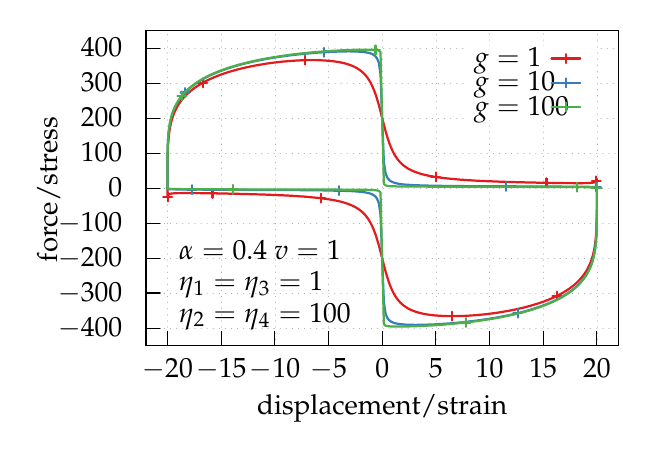
\begin{tikzpicture}[gnuplot]
%% generated with GNUPLOT 5.4p2 (Lua 5.4; terminal rev. Jun 2020, script rev. 114)
%% 11/05/21 19:26:08
\path (0.000,0.000) rectangle (6.000,4.000);
\gpcolor{color=gp lt color axes}
\gpsetlinetype{gp lt axes}
\gpsetdashtype{gp dt axes}
\gpsetlinewidth{0.50}
\draw[gp path] (0.000,0.222)--(5.999,0.222);
\gpcolor{color=gp lt color border}
\gpsetlinetype{gp lt border}
\gpsetdashtype{gp dt solid}
\gpsetlinewidth{1.00}
\draw[gp path] (0.000,0.222)--(0.180,0.222);
\node[gp node right] at (-0.184,0.222) {$-400$};
\gpcolor{color=gp lt color axes}
\gpsetlinetype{gp lt axes}
\gpsetdashtype{gp dt axes}
\gpsetlinewidth{0.50}
\draw[gp path] (0.000,0.667)--(5.999,0.667);
\gpcolor{color=gp lt color border}
\gpsetlinetype{gp lt border}
\gpsetdashtype{gp dt solid}
\gpsetlinewidth{1.00}
\draw[gp path] (0.000,0.667)--(0.180,0.667);
\node[gp node right] at (-0.184,0.667) {$-300$};
\gpcolor{color=gp lt color axes}
\gpsetlinetype{gp lt axes}
\gpsetdashtype{gp dt axes}
\gpsetlinewidth{0.50}
\draw[gp path] (0.000,1.111)--(5.999,1.111);
\gpcolor{color=gp lt color border}
\gpsetlinetype{gp lt border}
\gpsetdashtype{gp dt solid}
\gpsetlinewidth{1.00}
\draw[gp path] (0.000,1.111)--(0.180,1.111);
\node[gp node right] at (-0.184,1.111) {$-200$};
\gpcolor{color=gp lt color axes}
\gpsetlinetype{gp lt axes}
\gpsetdashtype{gp dt axes}
\gpsetlinewidth{0.50}
\draw[gp path] (0.000,1.555)--(5.999,1.555);
\gpcolor{color=gp lt color border}
\gpsetlinetype{gp lt border}
\gpsetdashtype{gp dt solid}
\gpsetlinewidth{1.00}
\draw[gp path] (0.000,1.555)--(0.180,1.555);
\node[gp node right] at (-0.184,1.555) {$-100$};
\gpcolor{color=gp lt color axes}
\gpsetlinetype{gp lt axes}
\gpsetdashtype{gp dt axes}
\gpsetlinewidth{0.50}
\draw[gp path] (0.000,2.000)--(5.999,2.000);
\gpcolor{color=gp lt color border}
\gpsetlinetype{gp lt border}
\gpsetdashtype{gp dt solid}
\gpsetlinewidth{1.00}
\draw[gp path] (0.000,2.000)--(0.180,2.000);
\node[gp node right] at (-0.184,2.000) {$0$};
\gpcolor{color=gp lt color axes}
\gpsetlinetype{gp lt axes}
\gpsetdashtype{gp dt axes}
\gpsetlinewidth{0.50}
\draw[gp path] (0.000,2.444)--(5.999,2.444);
\gpcolor{color=gp lt color border}
\gpsetlinetype{gp lt border}
\gpsetdashtype{gp dt solid}
\gpsetlinewidth{1.00}
\draw[gp path] (0.000,2.444)--(0.180,2.444);
\node[gp node right] at (-0.184,2.444) {$100$};
\gpcolor{color=gp lt color axes}
\gpsetlinetype{gp lt axes}
\gpsetdashtype{gp dt axes}
\gpsetlinewidth{0.50}
\draw[gp path] (0.000,2.888)--(4.047,2.888);
\draw[gp path] (5.699,2.888)--(5.999,2.888);
\gpcolor{color=gp lt color border}
\gpsetlinetype{gp lt border}
\gpsetdashtype{gp dt solid}
\gpsetlinewidth{1.00}
\draw[gp path] (0.000,2.888)--(0.180,2.888);
\node[gp node right] at (-0.184,2.888) {$200$};
\gpcolor{color=gp lt color axes}
\gpsetlinetype{gp lt axes}
\gpsetdashtype{gp dt axes}
\gpsetlinewidth{0.50}
\draw[gp path] (0.000,3.333)--(4.047,3.333);
\draw[gp path] (5.699,3.333)--(5.999,3.333);
\gpcolor{color=gp lt color border}
\gpsetlinetype{gp lt border}
\gpsetdashtype{gp dt solid}
\gpsetlinewidth{1.00}
\draw[gp path] (0.000,3.333)--(0.180,3.333);
\node[gp node right] at (-0.184,3.333) {$300$};
\gpcolor{color=gp lt color axes}
\gpsetlinetype{gp lt axes}
\gpsetdashtype{gp dt axes}
\gpsetlinewidth{0.50}
\draw[gp path] (0.000,3.777)--(4.047,3.777);
\draw[gp path] (5.699,3.777)--(5.999,3.777);
\gpcolor{color=gp lt color border}
\gpsetlinetype{gp lt border}
\gpsetdashtype{gp dt solid}
\gpsetlinewidth{1.00}
\draw[gp path] (0.000,3.777)--(0.180,3.777);
\node[gp node right] at (-0.184,3.777) {$400$};
\gpcolor{color=gp lt color axes}
\gpsetlinetype{gp lt axes}
\gpsetdashtype{gp dt axes}
\gpsetlinewidth{0.50}
\draw[gp path] (0.273,0.000)--(0.273,3.999);
\gpcolor{color=gp lt color border}
\gpsetlinetype{gp lt border}
\gpsetdashtype{gp dt solid}
\gpsetlinewidth{1.00}
\draw[gp path] (0.273,0.000)--(0.273,0.180);
\node[gp node center] at (0.273,-0.308) {$-20$};
\gpcolor{color=gp lt color axes}
\gpsetlinetype{gp lt axes}
\gpsetdashtype{gp dt axes}
\gpsetlinewidth{0.50}
\draw[gp path] (0.954,0.000)--(0.954,3.999);
\gpcolor{color=gp lt color border}
\gpsetlinetype{gp lt border}
\gpsetdashtype{gp dt solid}
\gpsetlinewidth{1.00}
\draw[gp path] (0.954,0.000)--(0.954,0.180);
\node[gp node center] at (0.954,-0.308) {$-15$};
\gpcolor{color=gp lt color axes}
\gpsetlinetype{gp lt axes}
\gpsetdashtype{gp dt axes}
\gpsetlinewidth{0.50}
\draw[gp path] (1.636,0.000)--(1.636,3.999);
\gpcolor{color=gp lt color border}
\gpsetlinetype{gp lt border}
\gpsetdashtype{gp dt solid}
\gpsetlinewidth{1.00}
\draw[gp path] (1.636,0.000)--(1.636,0.180);
\node[gp node center] at (1.636,-0.308) {$-10$};
\gpcolor{color=gp lt color axes}
\gpsetlinetype{gp lt axes}
\gpsetdashtype{gp dt axes}
\gpsetlinewidth{0.50}
\draw[gp path] (2.318,0.000)--(2.318,3.999);
\gpcolor{color=gp lt color border}
\gpsetlinetype{gp lt border}
\gpsetdashtype{gp dt solid}
\gpsetlinewidth{1.00}
\draw[gp path] (2.318,0.000)--(2.318,0.180);
\node[gp node center] at (2.318,-0.308) {$-5$};
\gpcolor{color=gp lt color axes}
\gpsetlinetype{gp lt axes}
\gpsetdashtype{gp dt axes}
\gpsetlinewidth{0.50}
\draw[gp path] (3.000,0.000)--(3.000,3.999);
\gpcolor{color=gp lt color border}
\gpsetlinetype{gp lt border}
\gpsetdashtype{gp dt solid}
\gpsetlinewidth{1.00}
\draw[gp path] (3.000,0.000)--(3.000,0.180);
\node[gp node center] at (3.000,-0.308) {$0$};
\gpcolor{color=gp lt color axes}
\gpsetlinetype{gp lt axes}
\gpsetdashtype{gp dt axes}
\gpsetlinewidth{0.50}
\draw[gp path] (3.681,0.000)--(3.681,3.999);
\gpcolor{color=gp lt color border}
\gpsetlinetype{gp lt border}
\gpsetdashtype{gp dt solid}
\gpsetlinewidth{1.00}
\draw[gp path] (3.681,0.000)--(3.681,0.180);
\node[gp node center] at (3.681,-0.308) {$5$};
\gpcolor{color=gp lt color axes}
\gpsetlinetype{gp lt axes}
\gpsetdashtype{gp dt axes}
\gpsetlinewidth{0.50}
\draw[gp path] (4.363,0.000)--(4.363,2.875);
\draw[gp path] (4.363,3.799)--(4.363,3.999);
\gpcolor{color=gp lt color border}
\gpsetlinetype{gp lt border}
\gpsetdashtype{gp dt solid}
\gpsetlinewidth{1.00}
\draw[gp path] (4.363,0.000)--(4.363,0.180);
\node[gp node center] at (4.363,-0.308) {$10$};
\gpcolor{color=gp lt color axes}
\gpsetlinetype{gp lt axes}
\gpsetdashtype{gp dt axes}
\gpsetlinewidth{0.50}
\draw[gp path] (5.045,0.000)--(5.045,2.875);
\draw[gp path] (5.045,3.799)--(5.045,3.999);
\gpcolor{color=gp lt color border}
\gpsetlinetype{gp lt border}
\gpsetdashtype{gp dt solid}
\gpsetlinewidth{1.00}
\draw[gp path] (5.045,0.000)--(5.045,0.180);
\node[gp node center] at (5.045,-0.308) {$15$};
\gpcolor{color=gp lt color axes}
\gpsetlinetype{gp lt axes}
\gpsetdashtype{gp dt axes}
\gpsetlinewidth{0.50}
\draw[gp path] (5.726,0.000)--(5.726,3.999);
\gpcolor{color=gp lt color border}
\gpsetlinetype{gp lt border}
\gpsetdashtype{gp dt solid}
\gpsetlinewidth{1.00}
\draw[gp path] (5.726,0.000)--(5.726,0.180);
\node[gp node center] at (5.726,-0.308) {$20$};
\draw[gp path] (0.000,3.999)--(0.000,0.000)--(5.999,0.000)--(5.999,3.999)--cycle;
\node[gp node left] at (0.300,1.200) {$\alpha=0.4$ $v=1$};
\node[gp node left] at (0.300,0.800) {$\eta_1=\eta_3=1$};
\node[gp node left] at (0.300,0.400) {$\eta_2=\eta_4=100$};
\node[gp node center,rotate=-270] at (-1.212,1.999) {force/stress};
\node[gp node center] at (2.999,-0.769) {displacement/strain};
\gpcolor{rgb color={0.894,0.102,0.110}}
\gpsetlinewidth{2.00}
\draw[gp path] (5.726,2.000)--(5.726,1.918)--(5.726,1.826)--(5.726,1.738)--(5.725,1.671)%
  --(5.724,1.624)--(5.723,1.582)--(5.722,1.544)--(5.721,1.509)--(5.720,1.477)--(5.718,1.447)%
  --(5.716,1.419)--(5.714,1.393)--(5.712,1.368)--(5.710,1.345)--(5.707,1.323)--(5.705,1.301)%
  --(5.702,1.281)--(5.699,1.261)--(5.696,1.242)--(5.693,1.224)--(5.689,1.207)--(5.686,1.190)%
  --(5.682,1.173)--(5.678,1.157)--(5.674,1.142)--(5.670,1.127)--(5.665,1.112)--(5.661,1.098)%
  --(5.656,1.084)--(5.651,1.070)--(5.646,1.057)--(5.641,1.044)--(5.635,1.031)--(5.630,1.019)%
  --(5.624,1.007)--(5.618,0.995)--(5.612,0.983)--(5.606,0.972)--(5.599,0.960)--(5.593,0.949)%
  --(5.586,0.938)--(5.579,0.928)--(5.572,0.917)--(5.565,0.907)--(5.558,0.897)--(5.550,0.887)%
  --(5.543,0.877)--(5.535,0.868)--(5.527,0.858)--(5.519,0.849)--(5.510,0.840)--(5.502,0.831)%
  --(5.493,0.822)--(5.485,0.813)--(5.476,0.804)--(5.467,0.796)--(5.458,0.788)--(5.448,0.779)%
  --(5.439,0.771)--(5.429,0.763)--(5.419,0.755)--(5.409,0.747)--(5.399,0.740)--(5.389,0.732)%
  --(5.379,0.725)--(5.368,0.717)--(5.357,0.710)--(5.347,0.703)--(5.336,0.696)--(5.324,0.689)%
  --(5.313,0.682)--(5.302,0.675)--(5.290,0.669)--(5.279,0.662)--(5.267,0.655)--(5.255,0.649)%
  --(5.243,0.643)--(5.230,0.636)--(5.218,0.630)--(5.206,0.624)--(5.193,0.618)--(5.180,0.612)%
  --(5.167,0.606)--(5.154,0.601)--(5.141,0.595)--(5.128,0.589)--(5.114,0.584)--(5.101,0.578)%
  --(5.087,0.573)--(5.073,0.568)--(5.059,0.562)--(5.045,0.557)--(5.031,0.552)--(5.016,0.547)%
  --(5.002,0.542)--(4.987,0.537)--(4.973,0.533)--(4.958,0.528)--(4.943,0.523)--(4.928,0.519)%
  --(4.912,0.514)--(4.897,0.510)--(4.882,0.505)--(4.866,0.501)--(4.850,0.497)--(4.835,0.492)%
  --(4.819,0.488)--(4.803,0.484)--(4.787,0.480)--(4.770,0.476)--(4.754,0.473)--(4.738,0.469)%
  --(4.721,0.465)--(4.704,0.461)--(4.688,0.458)--(4.671,0.454)--(4.654,0.451)--(4.637,0.448)%
  --(4.620,0.444)--(4.602,0.441)--(4.585,0.438)--(4.567,0.435)--(4.550,0.432)--(4.532,0.429)%
  --(4.514,0.426)--(4.497,0.423)--(4.479,0.420)--(4.461,0.417)--(4.442,0.415)--(4.424,0.412)%
  --(4.406,0.410)--(4.388,0.407)--(4.369,0.405)--(4.351,0.403)--(4.332,0.401)--(4.313,0.398)%
  --(4.294,0.396)--(4.275,0.394)--(4.256,0.392)--(4.237,0.391)--(4.218,0.389)--(4.199,0.387)%
  --(4.180,0.386)--(4.161,0.384)--(4.141,0.383)--(4.122,0.382)--(4.102,0.380)--(4.082,0.379)%
  --(4.063,0.378)--(4.043,0.377)--(4.023,0.376)--(4.003,0.376)--(3.983,0.375)--(3.963,0.375)%
  --(3.943,0.374)--(3.923,0.374)--(3.903,0.374)--(3.883,0.374)--(3.862,0.374)--(3.842,0.374)%
  --(3.822,0.374)--(3.801,0.375)--(3.781,0.376)--(3.760,0.377)--(3.740,0.378)--(3.719,0.379)%
  --(3.698,0.381)--(3.678,0.382)--(3.657,0.384)--(3.636,0.386)--(3.615,0.389)--(3.594,0.392)%
  --(3.573,0.395)--(3.552,0.398)--(3.531,0.402)--(3.510,0.407)--(3.489,0.411)--(3.468,0.417)%
  --(3.447,0.423)--(3.426,0.429)--(3.405,0.437)--(3.384,0.445)--(3.362,0.454)--(3.341,0.465)%
  --(3.320,0.476)--(3.299,0.490)--(3.277,0.505)--(3.256,0.522)--(3.235,0.541)--(3.213,0.564)%
  --(3.192,0.590)--(3.171,0.620)--(3.149,0.656)--(3.128,0.698)--(3.107,0.746)--(3.085,0.803)%
  --(3.064,0.869)--(3.042,0.943)--(3.021,1.024)--(2.999,1.109)--(2.978,1.193)--(2.957,1.274)%
  --(2.935,1.348)--(2.914,1.414)--(2.892,1.471)--(2.871,1.520)--(2.850,1.562)--(2.828,1.598)%
  --(2.807,1.629)--(2.786,1.655)--(2.764,1.679)--(2.743,1.699)--(2.722,1.716)--(2.700,1.732)%
  --(2.679,1.746)--(2.658,1.758)--(2.637,1.769)--(2.615,1.779)--(2.594,1.788)--(2.573,1.796)%
  --(2.552,1.804)--(2.531,1.811)--(2.510,1.817)--(2.489,1.823)--(2.468,1.829)--(2.447,1.834)%
  --(2.426,1.838)--(2.405,1.843)--(2.384,1.847)--(2.363,1.850)--(2.342,1.854)--(2.321,1.857)%
  --(2.301,1.861)--(2.280,1.864)--(2.259,1.866)--(2.239,1.869)--(2.218,1.872)--(2.198,1.874)%
  --(2.177,1.876)--(2.157,1.878)--(2.137,1.880)--(2.116,1.882)--(2.096,1.884)--(2.076,1.886)%
  --(2.056,1.888)--(2.036,1.889)--(2.016,1.891)--(1.996,1.893)--(1.976,1.894)--(1.956,1.895)%
  --(1.936,1.897)--(1.917,1.898)--(1.897,1.899)--(1.877,1.900)--(1.858,1.902)--(1.838,1.903)%
  --(1.819,1.904)--(1.800,1.905)--(1.781,1.906)--(1.762,1.907)--(1.743,1.908)--(1.724,1.909)%
  --(1.705,1.909)--(1.686,1.910)--(1.667,1.911)--(1.648,1.912)--(1.630,1.913)--(1.611,1.913)%
  --(1.593,1.914)--(1.575,1.915)--(1.557,1.916)--(1.538,1.916)--(1.520,1.917)--(1.502,1.918)%
  --(1.485,1.918)--(1.467,1.919)--(1.449,1.919)--(1.432,1.920)--(1.414,1.920)--(1.397,1.921)%
  --(1.379,1.921)--(1.362,1.922)--(1.345,1.922)--(1.328,1.923)--(1.311,1.923)--(1.295,1.924)%
  --(1.278,1.924)--(1.261,1.925)--(1.245,1.925)--(1.229,1.926)--(1.212,1.926)--(1.196,1.926)%
  --(1.180,1.927)--(1.164,1.927)--(1.149,1.927)--(1.133,1.928)--(1.117,1.928)--(1.102,1.929)%
  --(1.087,1.929)--(1.071,1.929)--(1.056,1.929)--(1.041,1.930)--(1.026,1.930)--(1.012,1.930)%
  --(0.997,1.931)--(0.983,1.931)--(0.968,1.931)--(0.954,1.931)--(0.940,1.932)--(0.926,1.932)%
  --(0.912,1.932)--(0.898,1.932)--(0.885,1.933)--(0.871,1.933)--(0.858,1.933)--(0.845,1.933)%
  --(0.832,1.934)--(0.819,1.934)--(0.806,1.934)--(0.793,1.934)--(0.781,1.934)--(0.769,1.934)%
  --(0.756,1.935)--(0.744,1.935)--(0.732,1.935)--(0.720,1.935)--(0.709,1.935)--(0.697,1.935)%
  --(0.686,1.936)--(0.675,1.936)--(0.663,1.936)--(0.652,1.936)--(0.642,1.936)--(0.631,1.936)%
  --(0.620,1.936)--(0.610,1.936)--(0.600,1.936)--(0.590,1.936)--(0.580,1.936)--(0.570,1.937)%
  --(0.560,1.937)--(0.551,1.937)--(0.541,1.937)--(0.532,1.937)--(0.523,1.937)--(0.514,1.937)%
  --(0.506,1.937)--(0.497,1.937)--(0.489,1.937)--(0.480,1.937)--(0.472,1.937)--(0.464,1.937)%
  --(0.456,1.937)--(0.449,1.936)--(0.441,1.936)--(0.434,1.936)--(0.427,1.936)--(0.420,1.936)%
  --(0.413,1.936)--(0.406,1.936)--(0.400,1.936)--(0.393,1.935)--(0.387,1.935)--(0.381,1.935)%
  --(0.375,1.935)--(0.369,1.934)--(0.364,1.934)--(0.358,1.934)--(0.353,1.933)--(0.348,1.933)%
  --(0.343,1.933)--(0.338,1.932)--(0.334,1.932)--(0.329,1.931)--(0.325,1.930)--(0.321,1.930)%
  --(0.317,1.929)--(0.313,1.928)--(0.310,1.927)--(0.306,1.926)--(0.303,1.925)--(0.300,1.924)%
  --(0.297,1.923)--(0.294,1.921)--(0.292,1.920)--(0.289,1.918)--(0.287,1.916)--(0.285,1.914)%
  --(0.283,1.911)--(0.281,1.908)--(0.279,1.905)--(0.278,1.901)--(0.277,1.897)--(0.276,1.892)%
  --(0.275,1.887)--(0.274,1.881)--(0.273,1.883)--(0.273,1.901)--(0.273,1.939)--(0.273,2.000)%
  --(0.273,2.081)--(0.273,2.173)--(0.273,2.261)--(0.274,2.328)--(0.275,2.375)--(0.276,2.417)%
  --(0.277,2.455)--(0.278,2.490)--(0.279,2.522)--(0.281,2.552)--(0.283,2.580)--(0.285,2.606)%
  --(0.287,2.631)--(0.289,2.654)--(0.292,2.676)--(0.294,2.698)--(0.297,2.718)--(0.300,2.738)%
  --(0.303,2.757)--(0.306,2.775)--(0.310,2.792)--(0.313,2.809)--(0.317,2.826)--(0.321,2.842)%
  --(0.325,2.857)--(0.329,2.872)--(0.334,2.887)--(0.338,2.901)--(0.343,2.915)--(0.348,2.929)%
  --(0.353,2.942)--(0.358,2.955)--(0.364,2.968)--(0.369,2.980)--(0.375,2.992)--(0.381,3.004)%
  --(0.387,3.016)--(0.393,3.027)--(0.400,3.039)--(0.406,3.050)--(0.413,3.061)--(0.420,3.071)%
  --(0.427,3.082)--(0.434,3.092)--(0.441,3.102)--(0.449,3.112)--(0.456,3.122)--(0.464,3.131)%
  --(0.472,3.141)--(0.480,3.150)--(0.489,3.159)--(0.497,3.168)--(0.506,3.177)--(0.514,3.186)%
  --(0.523,3.195)--(0.532,3.203)--(0.541,3.211)--(0.551,3.220)--(0.560,3.228)--(0.570,3.236)%
  --(0.580,3.244)--(0.590,3.252)--(0.600,3.259)--(0.610,3.267)--(0.620,3.274)--(0.631,3.282)%
  --(0.642,3.289)--(0.652,3.296)--(0.663,3.303)--(0.675,3.310)--(0.686,3.317)--(0.697,3.324)%
  --(0.709,3.330)--(0.720,3.337)--(0.732,3.344)--(0.744,3.350)--(0.756,3.356)--(0.769,3.363)%
  --(0.781,3.369)--(0.793,3.375)--(0.806,3.381)--(0.819,3.387)--(0.832,3.393)--(0.845,3.398)%
  --(0.858,3.404)--(0.871,3.410)--(0.885,3.415)--(0.898,3.421)--(0.912,3.426)--(0.926,3.431)%
  --(0.940,3.437)--(0.954,3.442)--(0.968,3.447)--(0.983,3.452)--(0.997,3.457)--(1.012,3.462)%
  --(1.026,3.466)--(1.041,3.471)--(1.056,3.476)--(1.071,3.480)--(1.087,3.485)--(1.102,3.489)%
  --(1.117,3.494)--(1.133,3.498)--(1.149,3.502)--(1.164,3.507)--(1.180,3.511)--(1.196,3.515)%
  --(1.212,3.519)--(1.229,3.523)--(1.245,3.526)--(1.261,3.530)--(1.278,3.534)--(1.295,3.538)%
  --(1.311,3.541)--(1.328,3.545)--(1.345,3.548)--(1.362,3.551)--(1.379,3.555)--(1.397,3.558)%
  --(1.414,3.561)--(1.432,3.564)--(1.449,3.567)--(1.467,3.570)--(1.485,3.573)--(1.502,3.576)%
  --(1.520,3.579)--(1.538,3.582)--(1.557,3.584)--(1.575,3.587)--(1.593,3.589)--(1.611,3.592)%
  --(1.630,3.594)--(1.648,3.596)--(1.667,3.598)--(1.686,3.601)--(1.705,3.603)--(1.724,3.605)%
  --(1.743,3.607)--(1.762,3.608)--(1.781,3.610)--(1.800,3.612)--(1.819,3.613)--(1.838,3.615)%
  --(1.858,3.616)--(1.877,3.617)--(1.897,3.619)--(1.917,3.620)--(1.936,3.621)--(1.956,3.622)%
  --(1.976,3.623)--(1.996,3.623)--(2.016,3.624)--(2.036,3.624)--(2.056,3.625)--(2.076,3.625)%
  --(2.096,3.625)--(2.116,3.625)--(2.137,3.625)--(2.157,3.625)--(2.177,3.625)--(2.198,3.624)%
  --(2.218,3.623)--(2.239,3.622)--(2.259,3.621)--(2.280,3.620)--(2.301,3.618)--(2.321,3.617)%
  --(2.342,3.615)--(2.363,3.613)--(2.384,3.610)--(2.405,3.607)--(2.426,3.604)--(2.447,3.601)%
  --(2.468,3.597)--(2.489,3.592)--(2.510,3.588)--(2.531,3.582)--(2.552,3.576)--(2.573,3.570)%
  --(2.594,3.562)--(2.615,3.554)--(2.637,3.545)--(2.658,3.534)--(2.679,3.523)--(2.700,3.509)%
  --(2.722,3.494)--(2.743,3.477)--(2.764,3.458)--(2.786,3.435)--(2.807,3.409)--(2.828,3.379)%
  --(2.850,3.343)--(2.871,3.301)--(2.892,3.253)--(2.914,3.196)--(2.935,3.130)--(2.957,3.056)%
  --(2.978,2.975)--(2.999,2.890)--(3.021,2.806)--(3.042,2.725)--(3.064,2.651)--(3.085,2.585)%
  --(3.107,2.528)--(3.128,2.479)--(3.149,2.437)--(3.171,2.401)--(3.192,2.370)--(3.213,2.344)%
  --(3.235,2.320)--(3.256,2.300)--(3.277,2.283)--(3.299,2.267)--(3.320,2.253)--(3.341,2.241)%
  --(3.362,2.230)--(3.384,2.220)--(3.405,2.211)--(3.426,2.203)--(3.447,2.195)--(3.468,2.188)%
  --(3.489,2.182)--(3.510,2.176)--(3.531,2.170)--(3.552,2.165)--(3.573,2.161)--(3.594,2.156)%
  --(3.615,2.152)--(3.636,2.149)--(3.657,2.145)--(3.678,2.142)--(3.698,2.138)--(3.719,2.135)%
  --(3.740,2.133)--(3.760,2.130)--(3.781,2.127)--(3.801,2.125)--(3.822,2.123)--(3.842,2.121)%
  --(3.862,2.119)--(3.883,2.117)--(3.903,2.115)--(3.923,2.113)--(3.943,2.111)--(3.963,2.110)%
  --(3.983,2.108)--(4.003,2.106)--(4.023,2.105)--(4.043,2.104)--(4.063,2.102)--(4.082,2.101)%
  --(4.102,2.100)--(4.122,2.099)--(4.141,2.097)--(4.161,2.096)--(4.180,2.095)--(4.199,2.094)%
  --(4.218,2.093)--(4.237,2.092)--(4.256,2.091)--(4.275,2.090)--(4.294,2.090)--(4.313,2.089)%
  --(4.332,2.088)--(4.351,2.087)--(4.369,2.086)--(4.388,2.086)--(4.406,2.085)--(4.424,2.084)%
  --(4.442,2.083)--(4.461,2.083)--(4.479,2.082)--(4.497,2.081)--(4.514,2.081)--(4.532,2.080)%
  --(4.550,2.080)--(4.567,2.079)--(4.585,2.079)--(4.602,2.078)--(4.620,2.078)--(4.637,2.077)%
  --(4.654,2.077)--(4.671,2.076)--(4.688,2.076)--(4.704,2.075)--(4.721,2.075)--(4.738,2.074)%
  --(4.754,2.074)--(4.770,2.073)--(4.787,2.073)--(4.803,2.073)--(4.819,2.072)--(4.835,2.072)%
  --(4.850,2.072)--(4.866,2.071)--(4.882,2.071)--(4.897,2.070)--(4.912,2.070)--(4.928,2.070)%
  --(4.943,2.070)--(4.958,2.069)--(4.973,2.069)--(4.987,2.069)--(5.002,2.068)--(5.016,2.068)%
  --(5.031,2.068)--(5.045,2.068)--(5.059,2.067)--(5.073,2.067)--(5.087,2.067)--(5.101,2.067)%
  --(5.114,2.066)--(5.128,2.066)--(5.141,2.066)--(5.154,2.066)--(5.167,2.065)--(5.180,2.065)%
  --(5.193,2.065)--(5.206,2.065)--(5.218,2.065)--(5.230,2.065)--(5.243,2.064)--(5.255,2.064)%
  --(5.267,2.064)--(5.279,2.064)--(5.290,2.064)--(5.302,2.064)--(5.313,2.063)--(5.324,2.063)%
  --(5.336,2.063)--(5.347,2.063)--(5.357,2.063)--(5.368,2.063)--(5.379,2.063)--(5.389,2.063)%
  --(5.399,2.063)--(5.409,2.063)--(5.419,2.063)--(5.429,2.062)--(5.439,2.062)--(5.448,2.062)%
  --(5.458,2.062)--(5.467,2.062)--(5.476,2.062)--(5.485,2.062)--(5.493,2.062)--(5.502,2.062)%
  --(5.510,2.062)--(5.519,2.062)--(5.527,2.062)--(5.535,2.062)--(5.543,2.062)--(5.550,2.063)%
  --(5.558,2.063)--(5.565,2.063)--(5.572,2.063)--(5.579,2.063)--(5.586,2.063)--(5.593,2.063)%
  --(5.599,2.063)--(5.606,2.064)--(5.612,2.064)--(5.618,2.064)--(5.624,2.064)--(5.630,2.065)%
  --(5.635,2.065)--(5.641,2.065)--(5.646,2.066)--(5.651,2.066)--(5.656,2.066)--(5.661,2.067)%
  --(5.665,2.067)--(5.670,2.068)--(5.674,2.069)--(5.678,2.069)--(5.682,2.070)--(5.686,2.071)%
  --(5.689,2.072)--(5.693,2.073)--(5.696,2.074)--(5.699,2.075)--(5.702,2.076)--(5.705,2.078)%
  --(5.707,2.079)--(5.710,2.081)--(5.712,2.083)--(5.714,2.085)--(5.716,2.088)--(5.718,2.091)%
  --(5.720,2.094)--(5.721,2.098)--(5.722,2.102)--(5.723,2.107)--(5.724,2.112)--(5.725,2.118)%
  --(5.726,2.116)--(5.726,2.098)--(5.726,2.060)--cycle;
\gpsetpointsize{4.00}
\gp3point{gp mark 1}{}{(5.726,2.000)}
\gp3point{gp mark 1}{}{(5.218,0.630)}
\gp3point{gp mark 1}{}{(3.883,0.374)}
\gp3point{gp mark 1}{}{(2.218,1.872)}
\gp3point{gp mark 1}{}{(0.845,1.933)}
\gp3point{gp mark 1}{}{(0.275,1.887)}
\gp3point{gp mark 1}{}{(0.720,3.337)}
\gp3point{gp mark 1}{}{(2.016,3.624)}
\gp3point{gp mark 1}{}{(3.678,2.142)}
\gp3point{gp mark 1}{}{(5.087,2.067)}
\gp3point{gp mark 1}{}{(5.718,2.091)}
\gpcolor{rgb color={0.216,0.494,0.722}}
\draw[gp path] (5.726,2.000)--(5.726,1.876)--(5.726,1.748)--(5.726,1.642)--(5.725,1.572)%
  --(5.724,1.529)--(5.723,1.492)--(5.722,1.458)--(5.721,1.427)--(5.720,1.398)--(5.718,1.371)%
  --(5.716,1.346)--(5.714,1.322)--(5.712,1.300)--(5.710,1.278)--(5.707,1.258)--(5.705,1.238)%
  --(5.702,1.219)--(5.699,1.201)--(5.696,1.183)--(5.693,1.166)--(5.689,1.150)--(5.686,1.134)%
  --(5.682,1.118)--(5.678,1.103)--(5.674,1.088)--(5.670,1.074)--(5.665,1.060)--(5.661,1.046)%
  --(5.656,1.032)--(5.651,1.019)--(5.646,1.007)--(5.641,0.994)--(5.635,0.982)--(5.630,0.970)%
  --(5.624,0.958)--(5.618,0.946)--(5.612,0.935)--(5.606,0.924)--(5.599,0.913)--(5.593,0.902)%
  --(5.586,0.891)--(5.579,0.881)--(5.572,0.871)--(5.565,0.861)--(5.558,0.851)--(5.550,0.841)%
  --(5.543,0.831)--(5.535,0.822)--(5.527,0.812)--(5.519,0.803)--(5.510,0.794)--(5.502,0.785)%
  --(5.493,0.776)--(5.485,0.768)--(5.476,0.759)--(5.467,0.751)--(5.458,0.742)--(5.448,0.734)%
  --(5.439,0.726)--(5.429,0.718)--(5.419,0.710)--(5.409,0.703)--(5.399,0.695)--(5.389,0.687)%
  --(5.379,0.680)--(5.368,0.672)--(5.357,0.665)--(5.347,0.658)--(5.336,0.651)--(5.324,0.644)%
  --(5.313,0.637)--(5.302,0.630)--(5.290,0.623)--(5.279,0.617)--(5.267,0.610)--(5.255,0.603)%
  --(5.243,0.597)--(5.230,0.591)--(5.218,0.584)--(5.206,0.578)--(5.193,0.572)--(5.180,0.566)%
  --(5.167,0.560)--(5.154,0.554)--(5.141,0.548)--(5.128,0.543)--(5.114,0.537)--(5.101,0.531)%
  --(5.087,0.526)--(5.073,0.520)--(5.059,0.515)--(5.045,0.510)--(5.031,0.504)--(5.016,0.499)%
  --(5.002,0.494)--(4.987,0.489)--(4.973,0.484)--(4.958,0.479)--(4.943,0.474)--(4.928,0.469)%
  --(4.912,0.464)--(4.897,0.460)--(4.882,0.455)--(4.866,0.450)--(4.850,0.446)--(4.835,0.441)%
  --(4.819,0.437)--(4.803,0.433)--(4.787,0.428)--(4.770,0.424)--(4.754,0.420)--(4.738,0.416)%
  --(4.721,0.412)--(4.704,0.408)--(4.688,0.404)--(4.671,0.400)--(4.654,0.396)--(4.637,0.392)%
  --(4.620,0.389)--(4.602,0.385)--(4.585,0.381)--(4.567,0.378)--(4.550,0.374)--(4.532,0.371)%
  --(4.514,0.367)--(4.497,0.364)--(4.479,0.361)--(4.461,0.357)--(4.442,0.354)--(4.424,0.351)%
  --(4.406,0.348)--(4.388,0.345)--(4.369,0.342)--(4.351,0.339)--(4.332,0.336)--(4.313,0.333)%
  --(4.294,0.331)--(4.275,0.328)--(4.256,0.325)--(4.237,0.323)--(4.218,0.320)--(4.199,0.317)%
  --(4.180,0.315)--(4.161,0.313)--(4.141,0.310)--(4.122,0.308)--(4.102,0.306)--(4.082,0.303)%
  --(4.063,0.301)--(4.043,0.299)--(4.023,0.297)--(4.003,0.295)--(3.983,0.293)--(3.963,0.291)%
  --(3.943,0.289)--(3.923,0.288)--(3.903,0.286)--(3.883,0.284)--(3.862,0.282)--(3.842,0.281)%
  --(3.822,0.279)--(3.801,0.278)--(3.781,0.277)--(3.760,0.275)--(3.740,0.274)--(3.719,0.273)%
  --(3.698,0.272)--(3.678,0.270)--(3.657,0.269)--(3.636,0.268)--(3.615,0.268)--(3.594,0.267)%
  --(3.573,0.266)--(3.552,0.265)--(3.531,0.265)--(3.510,0.264)--(3.489,0.264)--(3.468,0.264)%
  --(3.447,0.263)--(3.426,0.263)--(3.405,0.263)--(3.384,0.264)--(3.362,0.264)--(3.341,0.265)%
  --(3.320,0.265)--(3.299,0.266)--(3.277,0.268)--(3.256,0.270)--(3.235,0.272)--(3.213,0.274)%
  --(3.192,0.278)--(3.171,0.282)--(3.149,0.288)--(3.128,0.296)--(3.107,0.308)--(3.085,0.325)%
  --(3.064,0.353)--(3.042,0.408)--(3.021,0.552)--(2.999,1.109)--(2.978,1.666)--(2.957,1.809)%
  --(2.935,1.864)--(2.914,1.893)--(2.892,1.910)--(2.871,1.921)--(2.850,1.930)--(2.828,1.936)%
  --(2.807,1.941)--(2.786,1.945)--(2.764,1.948)--(2.743,1.951)--(2.722,1.953)--(2.700,1.955)%
  --(2.679,1.957)--(2.658,1.958)--(2.637,1.959)--(2.615,1.961)--(2.594,1.962)--(2.573,1.963)%
  --(2.552,1.963)--(2.531,1.964)--(2.510,1.965)--(2.489,1.965)--(2.468,1.966)--(2.447,1.967)%
  --(2.426,1.967)--(2.405,1.968)--(2.384,1.968)--(2.363,1.969)--(2.342,1.969)--(2.321,1.969)%
  --(2.301,1.970)--(2.280,1.970)--(2.259,1.970)--(2.239,1.971)--(2.218,1.971)--(2.198,1.971)%
  --(2.177,1.971)--(2.157,1.972)--(2.137,1.972)--(2.116,1.972)--(2.096,1.972)--(2.076,1.972)%
  --(2.056,1.973)--(2.036,1.973)--(2.016,1.973)--(1.996,1.973)--(1.976,1.973)--(1.956,1.974)%
  --(1.936,1.974)--(1.917,1.974)--(1.897,1.974)--(1.877,1.974)--(1.858,1.974)--(1.838,1.974)%
  --(1.819,1.975)--(1.800,1.975)--(1.781,1.975)--(1.762,1.975)--(1.743,1.975)--(1.724,1.975)%
  --(1.705,1.975)--(1.686,1.975)--(1.667,1.975)--(1.648,1.976)--(1.630,1.976)--(1.611,1.976)%
  --(1.593,1.976)--(1.575,1.976)--(1.557,1.976)--(1.538,1.976)--(1.520,1.976)--(1.502,1.976)%
  --(1.485,1.976)--(1.467,1.977)--(1.449,1.977)--(1.432,1.977)--(1.414,1.977)--(1.397,1.977)%
  --(1.379,1.977)--(1.362,1.977)--(1.345,1.977)--(1.328,1.977)--(1.311,1.977)--(1.295,1.977)%
  --(1.278,1.978)--(1.261,1.978)--(1.245,1.978)--(1.229,1.978)--(1.212,1.978)--(1.196,1.978)%
  --(1.180,1.978)--(1.164,1.978)--(1.149,1.978)--(1.133,1.978)--(1.117,1.978)--(1.102,1.978)%
  --(1.087,1.978)--(1.071,1.979)--(1.056,1.979)--(1.041,1.979)--(1.026,1.979)--(1.012,1.979)%
  --(0.997,1.979)--(0.983,1.979)--(0.968,1.979)--(0.954,1.979)--(0.940,1.979)--(0.926,1.979)%
  --(0.912,1.979)--(0.898,1.979)--(0.885,1.980)--(0.871,1.980)--(0.858,1.980)--(0.845,1.980)%
  --(0.832,1.980)--(0.819,1.980)--(0.806,1.980)--(0.793,1.980)--(0.781,1.980)--(0.769,1.980)%
  --(0.756,1.980)--(0.744,1.980)--(0.732,1.980)--(0.720,1.980)--(0.709,1.981)--(0.697,1.981)%
  --(0.686,1.981)--(0.675,1.981)--(0.663,1.981)--(0.652,1.981)--(0.642,1.981)--(0.631,1.981)%
  --(0.620,1.981)--(0.610,1.981)--(0.600,1.981)--(0.590,1.981)--(0.580,1.981)--(0.570,1.982)%
  --(0.560,1.982)--(0.551,1.982)--(0.541,1.982)--(0.532,1.982)--(0.523,1.982)--(0.514,1.982)%
  --(0.506,1.982)--(0.497,1.982)--(0.489,1.982)--(0.480,1.982)--(0.472,1.982)--(0.464,1.982)%
  --(0.456,1.983)--(0.449,1.983)--(0.441,1.983)--(0.434,1.983)--(0.427,1.983)--(0.420,1.983)%
  --(0.413,1.983)--(0.406,1.983)--(0.400,1.983)--(0.393,1.983)--(0.387,1.983)--(0.381,1.983)%
  --(0.375,1.983)--(0.369,1.984)--(0.364,1.984)--(0.358,1.984)--(0.353,1.984)--(0.348,1.984)%
  --(0.343,1.984)--(0.338,1.984)--(0.334,1.984)--(0.329,1.984)--(0.325,1.984)--(0.321,1.984)%
  --(0.317,1.984)--(0.313,1.984)--(0.310,1.984)--(0.306,1.984)--(0.303,1.984)--(0.300,1.984)%
  --(0.297,1.984)--(0.294,1.984)--(0.292,1.984)--(0.289,1.984)--(0.287,1.984)--(0.285,1.984)%
  --(0.283,1.984)--(0.281,1.984)--(0.279,1.984)--(0.278,1.983)--(0.277,1.983)--(0.276,1.982)%
  --(0.275,1.982)--(0.274,1.980)--(0.273,1.979)--(0.273,1.981)--(0.273,2.000)--(0.273,2.123)%
  --(0.273,2.251)--(0.273,2.357)--(0.274,2.427)--(0.275,2.470)--(0.276,2.507)--(0.277,2.541)%
  --(0.278,2.572)--(0.279,2.601)--(0.281,2.628)--(0.283,2.653)--(0.285,2.677)--(0.287,2.699)%
  --(0.289,2.721)--(0.292,2.741)--(0.294,2.761)--(0.297,2.780)--(0.300,2.798)--(0.303,2.816)%
  --(0.306,2.833)--(0.310,2.849)--(0.313,2.865)--(0.317,2.881)--(0.321,2.896)--(0.325,2.911)%
  --(0.329,2.925)--(0.334,2.939)--(0.338,2.953)--(0.343,2.967)--(0.348,2.980)--(0.353,2.992)%
  --(0.358,3.005)--(0.364,3.017)--(0.369,3.029)--(0.375,3.041)--(0.381,3.053)--(0.387,3.064)%
  --(0.393,3.075)--(0.400,3.086)--(0.406,3.097)--(0.413,3.108)--(0.420,3.118)--(0.427,3.128)%
  --(0.434,3.138)--(0.441,3.148)--(0.449,3.158)--(0.456,3.168)--(0.464,3.177)--(0.472,3.187)%
  --(0.480,3.196)--(0.489,3.205)--(0.497,3.214)--(0.506,3.223)--(0.514,3.231)--(0.523,3.240)%
  --(0.532,3.248)--(0.541,3.257)--(0.551,3.265)--(0.560,3.273)--(0.570,3.281)--(0.580,3.289)%
  --(0.590,3.296)--(0.600,3.304)--(0.610,3.312)--(0.620,3.319)--(0.631,3.327)--(0.642,3.334)%
  --(0.652,3.341)--(0.663,3.348)--(0.675,3.355)--(0.686,3.362)--(0.697,3.369)--(0.709,3.376)%
  --(0.720,3.382)--(0.732,3.389)--(0.744,3.396)--(0.756,3.402)--(0.769,3.408)--(0.781,3.415)%
  --(0.793,3.421)--(0.806,3.427)--(0.819,3.433)--(0.832,3.439)--(0.845,3.445)--(0.858,3.451)%
  --(0.871,3.456)--(0.885,3.462)--(0.898,3.468)--(0.912,3.473)--(0.926,3.479)--(0.940,3.484)%
  --(0.954,3.489)--(0.968,3.495)--(0.983,3.500)--(0.997,3.505)--(1.012,3.510)--(1.026,3.515)%
  --(1.041,3.520)--(1.056,3.525)--(1.071,3.530)--(1.087,3.535)--(1.102,3.539)--(1.117,3.544)%
  --(1.133,3.549)--(1.149,3.553)--(1.164,3.558)--(1.180,3.562)--(1.196,3.566)--(1.212,3.571)%
  --(1.229,3.575)--(1.245,3.579)--(1.261,3.583)--(1.278,3.587)--(1.295,3.591)--(1.311,3.595)%
  --(1.328,3.599)--(1.345,3.603)--(1.362,3.607)--(1.379,3.610)--(1.397,3.614)--(1.414,3.618)%
  --(1.432,3.621)--(1.449,3.625)--(1.467,3.628)--(1.485,3.632)--(1.502,3.635)--(1.520,3.638)%
  --(1.538,3.642)--(1.557,3.645)--(1.575,3.648)--(1.593,3.651)--(1.611,3.654)--(1.630,3.657)%
  --(1.648,3.660)--(1.667,3.663)--(1.686,3.666)--(1.705,3.668)--(1.724,3.671)--(1.743,3.674)%
  --(1.762,3.676)--(1.781,3.679)--(1.800,3.682)--(1.819,3.684)--(1.838,3.686)--(1.858,3.689)%
  --(1.877,3.691)--(1.897,3.693)--(1.917,3.696)--(1.936,3.698)--(1.956,3.700)--(1.976,3.702)%
  --(1.996,3.704)--(2.016,3.706)--(2.036,3.708)--(2.056,3.710)--(2.076,3.711)--(2.096,3.713)%
  --(2.116,3.715)--(2.137,3.717)--(2.157,3.718)--(2.177,3.720)--(2.198,3.721)--(2.218,3.722)%
  --(2.239,3.724)--(2.259,3.725)--(2.280,3.726)--(2.301,3.727)--(2.321,3.729)--(2.342,3.730)%
  --(2.363,3.731)--(2.384,3.731)--(2.405,3.732)--(2.426,3.733)--(2.447,3.734)--(2.468,3.734)%
  --(2.489,3.735)--(2.510,3.735)--(2.531,3.735)--(2.552,3.736)--(2.573,3.736)--(2.594,3.736)%
  --(2.615,3.735)--(2.637,3.735)--(2.658,3.734)--(2.679,3.734)--(2.700,3.733)--(2.722,3.731)%
  --(2.743,3.729)--(2.764,3.727)--(2.786,3.725)--(2.807,3.721)--(2.828,3.717)--(2.850,3.711)%
  --(2.871,3.703)--(2.892,3.691)--(2.914,3.674)--(2.935,3.646)--(2.957,3.591)--(2.978,3.447)%
  --(2.999,2.890)--(3.021,2.333)--(3.042,2.190)--(3.064,2.135)--(3.085,2.106)--(3.107,2.089)%
  --(3.128,2.078)--(3.149,2.069)--(3.171,2.063)--(3.192,2.058)--(3.213,2.054)--(3.235,2.051)%
  --(3.256,2.048)--(3.277,2.046)--(3.299,2.044)--(3.320,2.042)--(3.341,2.041)--(3.362,2.040)%
  --(3.384,2.038)--(3.405,2.037)--(3.426,2.036)--(3.447,2.036)--(3.468,2.035)--(3.489,2.034)%
  --(3.510,2.034)--(3.531,2.033)--(3.552,2.032)--(3.573,2.032)--(3.594,2.031)--(3.615,2.031)%
  --(3.636,2.030)--(3.657,2.030)--(3.678,2.030)--(3.698,2.029)--(3.719,2.029)--(3.740,2.029)%
  --(3.760,2.028)--(3.781,2.028)--(3.801,2.028)--(3.822,2.028)--(3.842,2.027)--(3.862,2.027)%
  --(3.883,2.027)--(3.903,2.027)--(3.923,2.027)--(3.943,2.026)--(3.963,2.026)--(3.983,2.026)%
  --(4.003,2.026)--(4.023,2.026)--(4.043,2.025)--(4.063,2.025)--(4.082,2.025)--(4.102,2.025)%
  --(4.122,2.025)--(4.141,2.025)--(4.161,2.025)--(4.180,2.024)--(4.199,2.024)--(4.218,2.024)%
  --(4.237,2.024)--(4.256,2.024)--(4.275,2.024)--(4.294,2.024)--(4.313,2.024)--(4.332,2.024)%
  --(4.351,2.023)--(4.369,2.023)--(4.388,2.023)--(4.406,2.023)--(4.424,2.023)--(4.442,2.023)%
  --(4.461,2.023)--(4.479,2.023)--(4.497,2.023)--(4.514,2.023)--(4.532,2.022)--(4.550,2.022)%
  --(4.567,2.022)--(4.585,2.022)--(4.602,2.022)--(4.620,2.022)--(4.637,2.022)--(4.654,2.022)%
  --(4.671,2.022)--(4.688,2.022)--(4.704,2.022)--(4.721,2.021)--(4.738,2.021)--(4.754,2.021)%
  --(4.770,2.021)--(4.787,2.021)--(4.803,2.021)--(4.819,2.021)--(4.835,2.021)--(4.850,2.021)%
  --(4.866,2.021)--(4.882,2.021)--(4.897,2.021)--(4.912,2.021)--(4.928,2.020)--(4.943,2.020)%
  --(4.958,2.020)--(4.973,2.020)--(4.987,2.020)--(5.002,2.020)--(5.016,2.020)--(5.031,2.020)%
  --(5.045,2.020)--(5.059,2.020)--(5.073,2.020)--(5.087,2.020)--(5.101,2.020)--(5.114,2.019)%
  --(5.128,2.019)--(5.141,2.019)--(5.154,2.019)--(5.167,2.019)--(5.180,2.019)--(5.193,2.019)%
  --(5.206,2.019)--(5.218,2.019)--(5.230,2.019)--(5.243,2.019)--(5.255,2.019)--(5.267,2.019)%
  --(5.279,2.019)--(5.290,2.018)--(5.302,2.018)--(5.313,2.018)--(5.324,2.018)--(5.336,2.018)%
  --(5.347,2.018)--(5.357,2.018)--(5.368,2.018)--(5.379,2.018)--(5.389,2.018)--(5.399,2.018)%
  --(5.409,2.018)--(5.419,2.018)--(5.429,2.017)--(5.439,2.017)--(5.448,2.017)--(5.458,2.017)%
  --(5.467,2.017)--(5.476,2.017)--(5.485,2.017)--(5.493,2.017)--(5.502,2.017)--(5.510,2.017)%
  --(5.519,2.017)--(5.527,2.017)--(5.535,2.017)--(5.543,2.016)--(5.550,2.016)--(5.558,2.016)%
  --(5.565,2.016)--(5.572,2.016)--(5.579,2.016)--(5.586,2.016)--(5.593,2.016)--(5.599,2.016)%
  --(5.606,2.016)--(5.612,2.016)--(5.618,2.016)--(5.624,2.016)--(5.630,2.015)--(5.635,2.015)%
  --(5.641,2.015)--(5.646,2.015)--(5.651,2.015)--(5.656,2.015)--(5.661,2.015)--(5.665,2.015)%
  --(5.670,2.015)--(5.674,2.015)--(5.678,2.015)--(5.682,2.015)--(5.686,2.015)--(5.689,2.015)%
  --(5.693,2.015)--(5.696,2.015)--(5.699,2.015)--(5.702,2.015)--(5.705,2.015)--(5.707,2.015)%
  --(5.710,2.015)--(5.712,2.015)--(5.714,2.015)--(5.716,2.015)--(5.718,2.015)--(5.720,2.015)%
  --(5.721,2.016)--(5.722,2.016)--(5.723,2.017)--(5.724,2.017)--(5.725,2.019)--(5.726,2.020)%
  --(5.726,2.018)--cycle;
\gp3point{gp mark 1}{}{(5.726,2.000)}
\gp3point{gp mark 1}{}{(4.721,0.412)}
\gp3point{gp mark 1}{}{(2.447,1.967)}
\gp3point{gp mark 1}{}{(0.580,1.981)}
\gp3point{gp mark 1}{}{(0.497,3.214)}
\gp3point{gp mark 1}{}{(2.259,3.725)}
\gp3point{gp mark 1}{}{(4.567,2.022)}
\gp3point{gp mark 1}{}{(5.720,2.015)}
\gpcolor{rgb color={0.302,0.686,0.290}}
\draw[gp path] (5.726,2.000)--(5.726,1.861)--(5.726,1.732)--(5.726,1.628)--(5.725,1.559)%
  --(5.724,1.518)--(5.723,1.481)--(5.722,1.448)--(5.721,1.417)--(5.720,1.389)--(5.718,1.363)%
  --(5.716,1.338)--(5.714,1.315)--(5.712,1.293)--(5.710,1.271)--(5.707,1.251)--(5.705,1.231)%
  --(5.702,1.213)--(5.699,1.195)--(5.696,1.177)--(5.693,1.160)--(5.689,1.144)--(5.686,1.128)%
  --(5.682,1.112)--(5.678,1.097)--(5.674,1.082)--(5.670,1.068)--(5.665,1.054)--(5.661,1.041)%
  --(5.656,1.027)--(5.651,1.014)--(5.646,1.001)--(5.641,0.989)--(5.635,0.977)--(5.630,0.965)%
  --(5.624,0.953)--(5.618,0.941)--(5.612,0.930)--(5.606,0.919)--(5.599,0.908)--(5.593,0.897)%
  --(5.586,0.886)--(5.579,0.876)--(5.572,0.866)--(5.565,0.856)--(5.558,0.846)--(5.550,0.836)%
  --(5.543,0.827)--(5.535,0.817)--(5.527,0.808)--(5.519,0.799)--(5.510,0.790)--(5.502,0.781)%
  --(5.493,0.772)--(5.485,0.763)--(5.476,0.755)--(5.467,0.746)--(5.458,0.738)--(5.448,0.730)%
  --(5.439,0.722)--(5.429,0.714)--(5.419,0.706)--(5.409,0.698)--(5.399,0.690)--(5.389,0.683)%
  --(5.379,0.675)--(5.368,0.668)--(5.357,0.661)--(5.347,0.653)--(5.336,0.646)--(5.324,0.639)%
  --(5.313,0.632)--(5.302,0.625)--(5.290,0.619)--(5.279,0.612)--(5.267,0.605)--(5.255,0.599)%
  --(5.243,0.592)--(5.230,0.586)--(5.218,0.580)--(5.206,0.574)--(5.193,0.567)--(5.180,0.561)%
  --(5.167,0.555)--(5.154,0.549)--(5.141,0.544)--(5.128,0.538)--(5.114,0.532)--(5.101,0.527)%
  --(5.087,0.521)--(5.073,0.516)--(5.059,0.510)--(5.045,0.505)--(5.031,0.499)--(5.016,0.494)%
  --(5.002,0.489)--(4.987,0.484)--(4.973,0.479)--(4.958,0.474)--(4.943,0.469)--(4.928,0.464)%
  --(4.912,0.459)--(4.897,0.455)--(4.882,0.450)--(4.866,0.445)--(4.850,0.441)--(4.835,0.436)%
  --(4.819,0.432)--(4.803,0.427)--(4.787,0.423)--(4.770,0.419)--(4.754,0.415)--(4.738,0.411)%
  --(4.721,0.406)--(4.704,0.402)--(4.688,0.398)--(4.671,0.394)--(4.654,0.391)--(4.637,0.387)%
  --(4.620,0.383)--(4.602,0.379)--(4.585,0.376)--(4.567,0.372)--(4.550,0.368)--(4.532,0.365)%
  --(4.514,0.361)--(4.497,0.358)--(4.479,0.355)--(4.461,0.351)--(4.442,0.348)--(4.424,0.345)%
  --(4.406,0.342)--(4.388,0.339)--(4.369,0.336)--(4.351,0.333)--(4.332,0.330)--(4.313,0.327)%
  --(4.294,0.324)--(4.275,0.321)--(4.256,0.318)--(4.237,0.316)--(4.218,0.313)--(4.199,0.310)%
  --(4.180,0.308)--(4.161,0.305)--(4.141,0.303)--(4.122,0.300)--(4.102,0.298)--(4.082,0.296)%
  --(4.063,0.293)--(4.043,0.291)--(4.023,0.289)--(4.003,0.287)--(3.983,0.285)--(3.963,0.283)%
  --(3.943,0.281)--(3.923,0.279)--(3.903,0.277)--(3.883,0.275)--(3.862,0.273)--(3.842,0.271)%
  --(3.822,0.270)--(3.801,0.268)--(3.781,0.266)--(3.760,0.265)--(3.740,0.263)--(3.719,0.262)%
  --(3.698,0.260)--(3.678,0.259)--(3.657,0.258)--(3.636,0.256)--(3.615,0.255)--(3.594,0.254)%
  --(3.573,0.253)--(3.552,0.252)--(3.531,0.250)--(3.510,0.249)--(3.489,0.248)--(3.468,0.248)%
  --(3.447,0.247)--(3.426,0.246)--(3.405,0.245)--(3.384,0.244)--(3.362,0.244)--(3.341,0.243)%
  --(3.320,0.243)--(3.299,0.242)--(3.277,0.242)--(3.256,0.241)--(3.235,0.241)--(3.213,0.241)%
  --(3.192,0.241)--(3.171,0.241)--(3.149,0.242)--(3.128,0.242)--(3.107,0.243)--(3.085,0.245)%
  --(3.064,0.247)--(3.042,0.253)--(3.021,0.271)--(2.999,1.109)--(2.978,1.946)--(2.957,1.964)%
  --(2.935,1.970)--(2.914,1.973)--(2.892,1.975)--(2.871,1.976)--(2.850,1.977)--(2.828,1.977)%
  --(2.807,1.978)--(2.786,1.978)--(2.764,1.978)--(2.743,1.979)--(2.722,1.979)--(2.700,1.979)%
  --(2.679,1.979)--(2.658,1.980)--(2.637,1.980)--(2.615,1.980)--(2.594,1.980)--(2.573,1.980)%
  --(2.552,1.980)--(2.531,1.980)--(2.510,1.980)--(2.489,1.980)--(2.468,1.980)--(2.447,1.980)%
  --(2.426,1.981)--(2.405,1.981)--(2.384,1.981)--(2.363,1.981)--(2.342,1.981)--(2.321,1.981)%
  --(2.301,1.981)--(2.280,1.981)--(2.259,1.981)--(2.239,1.981)--(2.218,1.981)--(2.198,1.981)%
  --(2.177,1.981)--(2.157,1.981)--(2.137,1.981)--(2.116,1.981)--(2.096,1.981)--(2.076,1.981)%
  --(2.056,1.981)--(2.036,1.981)--(2.016,1.981)--(1.996,1.981)--(1.976,1.981)--(1.956,1.982)%
  --(1.936,1.982)--(1.917,1.982)--(1.897,1.982)--(1.877,1.982)--(1.858,1.982)--(1.838,1.982)%
  --(1.819,1.982)--(1.800,1.982)--(1.781,1.982)--(1.762,1.982)--(1.743,1.982)--(1.724,1.982)%
  --(1.705,1.982)--(1.686,1.982)--(1.667,1.982)--(1.648,1.982)--(1.630,1.982)--(1.611,1.982)%
  --(1.593,1.982)--(1.575,1.982)--(1.557,1.982)--(1.538,1.982)--(1.520,1.982)--(1.502,1.982)%
  --(1.485,1.982)--(1.467,1.982)--(1.449,1.983)--(1.432,1.983)--(1.414,1.983)--(1.397,1.983)%
  --(1.379,1.983)--(1.362,1.983)--(1.345,1.983)--(1.328,1.983)--(1.311,1.983)--(1.295,1.983)%
  --(1.278,1.983)--(1.261,1.983)--(1.245,1.983)--(1.229,1.983)--(1.212,1.983)--(1.196,1.983)%
  --(1.180,1.983)--(1.164,1.983)--(1.149,1.983)--(1.133,1.983)--(1.117,1.983)--(1.102,1.983)%
  --(1.087,1.984)--(1.071,1.984)--(1.056,1.984)--(1.041,1.984)--(1.026,1.984)--(1.012,1.984)%
  --(0.997,1.984)--(0.983,1.984)--(0.968,1.984)--(0.954,1.984)--(0.940,1.984)--(0.926,1.984)%
  --(0.912,1.984)--(0.898,1.984)--(0.885,1.984)--(0.871,1.984)--(0.858,1.984)--(0.845,1.984)%
  --(0.832,1.985)--(0.819,1.985)--(0.806,1.985)--(0.793,1.985)--(0.781,1.985)--(0.769,1.985)%
  --(0.756,1.985)--(0.744,1.985)--(0.732,1.985)--(0.720,1.985)--(0.709,1.985)--(0.697,1.985)%
  --(0.686,1.985)--(0.675,1.985)--(0.663,1.985)--(0.652,1.986)--(0.642,1.986)--(0.631,1.986)%
  --(0.620,1.986)--(0.610,1.986)--(0.600,1.986)--(0.590,1.986)--(0.580,1.986)--(0.570,1.986)%
  --(0.560,1.986)--(0.551,1.986)--(0.541,1.986)--(0.532,1.986)--(0.523,1.987)--(0.514,1.987)%
  --(0.506,1.987)--(0.497,1.987)--(0.489,1.987)--(0.480,1.987)--(0.472,1.987)--(0.464,1.987)%
  --(0.456,1.987)--(0.449,1.987)--(0.441,1.987)--(0.434,1.988)--(0.427,1.988)--(0.420,1.988)%
  --(0.413,1.988)--(0.406,1.988)--(0.400,1.988)--(0.393,1.988)--(0.387,1.988)--(0.381,1.988)%
  --(0.375,1.988)--(0.369,1.989)--(0.364,1.989)--(0.358,1.989)--(0.353,1.989)--(0.348,1.989)%
  --(0.343,1.989)--(0.338,1.989)--(0.334,1.989)--(0.329,1.990)--(0.325,1.990)--(0.321,1.990)%
  --(0.317,1.990)--(0.313,1.990)--(0.310,1.990)--(0.306,1.990)--(0.303,1.991)--(0.300,1.991)%
  --(0.297,1.991)--(0.294,1.991)--(0.292,1.991)--(0.289,1.991)--(0.287,1.992)--(0.285,1.992)%
  --(0.283,1.992)--(0.281,1.992)--(0.279,1.992)--(0.278,1.993)--(0.277,1.993)--(0.276,1.993)%
  --(0.275,1.993)--(0.274,1.994)--(0.273,1.994)--(0.273,1.995)--(0.273,1.996)--(0.273,2.000)%
  --(0.273,2.138)--(0.273,2.267)--(0.273,2.371)--(0.274,2.440)--(0.275,2.481)--(0.276,2.518)%
  --(0.277,2.551)--(0.278,2.582)--(0.279,2.610)--(0.281,2.636)--(0.283,2.661)--(0.285,2.684)%
  --(0.287,2.706)--(0.289,2.728)--(0.292,2.748)--(0.294,2.768)--(0.297,2.786)--(0.300,2.804)%
  --(0.303,2.822)--(0.306,2.839)--(0.310,2.855)--(0.313,2.871)--(0.317,2.887)--(0.321,2.902)%
  --(0.325,2.917)--(0.329,2.931)--(0.334,2.945)--(0.338,2.958)--(0.343,2.972)--(0.348,2.985)%
  --(0.353,2.998)--(0.358,3.010)--(0.364,3.022)--(0.369,3.034)--(0.375,3.046)--(0.381,3.058)%
  --(0.387,3.069)--(0.393,3.080)--(0.400,3.091)--(0.406,3.102)--(0.413,3.113)--(0.420,3.123)%
  --(0.427,3.133)--(0.434,3.143)--(0.441,3.153)--(0.449,3.163)--(0.456,3.172)--(0.464,3.182)%
  --(0.472,3.191)--(0.480,3.200)--(0.489,3.209)--(0.497,3.218)--(0.506,3.227)--(0.514,3.236)%
  --(0.523,3.244)--(0.532,3.253)--(0.541,3.261)--(0.551,3.269)--(0.560,3.277)--(0.570,3.285)%
  --(0.580,3.293)--(0.590,3.301)--(0.600,3.309)--(0.610,3.316)--(0.620,3.324)--(0.631,3.331)%
  --(0.642,3.338)--(0.652,3.346)--(0.663,3.353)--(0.675,3.360)--(0.686,3.367)--(0.697,3.374)%
  --(0.709,3.380)--(0.720,3.387)--(0.732,3.394)--(0.744,3.400)--(0.756,3.407)--(0.769,3.413)%
  --(0.781,3.419)--(0.793,3.425)--(0.806,3.432)--(0.819,3.438)--(0.832,3.444)--(0.845,3.450)%
  --(0.858,3.455)--(0.871,3.461)--(0.885,3.467)--(0.898,3.472)--(0.912,3.478)--(0.926,3.483)%
  --(0.940,3.489)--(0.954,3.494)--(0.968,3.500)--(0.983,3.505)--(0.997,3.510)--(1.012,3.515)%
  --(1.026,3.520)--(1.041,3.525)--(1.056,3.530)--(1.071,3.535)--(1.087,3.540)--(1.102,3.544)%
  --(1.117,3.549)--(1.133,3.554)--(1.149,3.558)--(1.164,3.563)--(1.180,3.567)--(1.196,3.572)%
  --(1.212,3.576)--(1.229,3.580)--(1.245,3.584)--(1.261,3.588)--(1.278,3.593)--(1.295,3.597)%
  --(1.311,3.601)--(1.328,3.605)--(1.345,3.608)--(1.362,3.612)--(1.379,3.616)--(1.397,3.620)%
  --(1.414,3.623)--(1.432,3.627)--(1.449,3.631)--(1.467,3.634)--(1.485,3.638)--(1.502,3.641)%
  --(1.520,3.644)--(1.538,3.648)--(1.557,3.651)--(1.575,3.654)--(1.593,3.657)--(1.611,3.660)%
  --(1.630,3.663)--(1.648,3.666)--(1.667,3.669)--(1.686,3.672)--(1.705,3.675)--(1.724,3.678)%
  --(1.743,3.681)--(1.762,3.683)--(1.781,3.686)--(1.800,3.689)--(1.819,3.691)--(1.838,3.694)%
  --(1.858,3.696)--(1.877,3.699)--(1.897,3.701)--(1.917,3.703)--(1.936,3.706)--(1.956,3.708)%
  --(1.976,3.710)--(1.996,3.712)--(2.016,3.714)--(2.036,3.716)--(2.056,3.718)--(2.076,3.720)%
  --(2.096,3.722)--(2.116,3.724)--(2.137,3.726)--(2.157,3.728)--(2.177,3.729)--(2.198,3.731)%
  --(2.218,3.733)--(2.239,3.734)--(2.259,3.736)--(2.280,3.737)--(2.301,3.739)--(2.321,3.740)%
  --(2.342,3.741)--(2.363,3.743)--(2.384,3.744)--(2.405,3.745)--(2.426,3.746)--(2.447,3.747)%
  --(2.468,3.749)--(2.489,3.750)--(2.510,3.751)--(2.531,3.751)--(2.552,3.752)--(2.573,3.753)%
  --(2.594,3.754)--(2.615,3.755)--(2.637,3.755)--(2.658,3.756)--(2.679,3.756)--(2.700,3.757)%
  --(2.722,3.757)--(2.743,3.758)--(2.764,3.758)--(2.786,3.758)--(2.807,3.758)--(2.828,3.758)%
  --(2.850,3.757)--(2.871,3.757)--(2.892,3.756)--(2.914,3.754)--(2.935,3.752)--(2.957,3.746)%
  --(2.978,3.728)--(2.999,2.890)--(3.021,2.053)--(3.042,2.035)--(3.064,2.029)--(3.085,2.026)%
  --(3.107,2.024)--(3.128,2.023)--(3.149,2.022)--(3.171,2.022)--(3.192,2.021)--(3.213,2.021)%
  --(3.235,2.021)--(3.256,2.020)--(3.277,2.020)--(3.299,2.020)--(3.320,2.020)--(3.341,2.019)%
  --(3.362,2.019)--(3.384,2.019)--(3.405,2.019)--(3.426,2.019)--(3.447,2.019)--(3.468,2.019)%
  --(3.489,2.019)--(3.510,2.019)--(3.531,2.019)--(3.552,2.019)--(3.573,2.018)--(3.594,2.018)%
  --(3.615,2.018)--(3.636,2.018)--(3.657,2.018)--(3.678,2.018)--(3.698,2.018)--(3.719,2.018)%
  --(3.740,2.018)--(3.760,2.018)--(3.781,2.018)--(3.801,2.018)--(3.822,2.018)--(3.842,2.018)%
  --(3.862,2.018)--(3.883,2.018)--(3.903,2.018)--(3.923,2.018)--(3.943,2.018)--(3.963,2.018)%
  --(3.983,2.018)--(4.003,2.018)--(4.023,2.018)--(4.043,2.017)--(4.063,2.017)--(4.082,2.017)%
  --(4.102,2.017)--(4.122,2.017)--(4.141,2.017)--(4.161,2.017)--(4.180,2.017)--(4.199,2.017)%
  --(4.218,2.017)--(4.237,2.017)--(4.256,2.017)--(4.275,2.017)--(4.294,2.017)--(4.313,2.017)%
  --(4.332,2.017)--(4.351,2.017)--(4.369,2.017)--(4.388,2.017)--(4.406,2.017)--(4.424,2.017)%
  --(4.442,2.017)--(4.461,2.017)--(4.479,2.017)--(4.497,2.017)--(4.514,2.017)--(4.532,2.017)%
  --(4.550,2.016)--(4.567,2.016)--(4.585,2.016)--(4.602,2.016)--(4.620,2.016)--(4.637,2.016)%
  --(4.654,2.016)--(4.671,2.016)--(4.688,2.016)--(4.704,2.016)--(4.721,2.016)--(4.738,2.016)%
  --(4.754,2.016)--(4.770,2.016)--(4.787,2.016)--(4.803,2.016)--(4.819,2.016)--(4.835,2.016)%
  --(4.850,2.016)--(4.866,2.016)--(4.882,2.016)--(4.897,2.016)--(4.912,2.015)--(4.928,2.015)%
  --(4.943,2.015)--(4.958,2.015)--(4.973,2.015)--(4.987,2.015)--(5.002,2.015)--(5.016,2.015)%
  --(5.031,2.015)--(5.045,2.015)--(5.059,2.015)--(5.073,2.015)--(5.087,2.015)--(5.101,2.015)%
  --(5.114,2.015)--(5.128,2.015)--(5.141,2.015)--(5.154,2.015)--(5.167,2.014)--(5.180,2.014)%
  --(5.193,2.014)--(5.206,2.014)--(5.218,2.014)--(5.230,2.014)--(5.243,2.014)--(5.255,2.014)%
  --(5.267,2.014)--(5.279,2.014)--(5.290,2.014)--(5.302,2.014)--(5.313,2.014)--(5.324,2.014)%
  --(5.336,2.014)--(5.347,2.013)--(5.357,2.013)--(5.368,2.013)--(5.379,2.013)--(5.389,2.013)%
  --(5.399,2.013)--(5.409,2.013)--(5.419,2.013)--(5.429,2.013)--(5.439,2.013)--(5.448,2.013)%
  --(5.458,2.013)--(5.467,2.013)--(5.476,2.012)--(5.485,2.012)--(5.493,2.012)--(5.502,2.012)%
  --(5.510,2.012)--(5.519,2.012)--(5.527,2.012)--(5.535,2.012)--(5.543,2.012)--(5.550,2.012)%
  --(5.558,2.012)--(5.565,2.011)--(5.572,2.011)--(5.579,2.011)--(5.586,2.011)--(5.593,2.011)%
  --(5.599,2.011)--(5.606,2.011)--(5.612,2.011)--(5.618,2.011)--(5.624,2.011)--(5.630,2.010)%
  --(5.635,2.010)--(5.641,2.010)--(5.646,2.010)--(5.651,2.010)--(5.656,2.010)--(5.661,2.010)%
  --(5.665,2.010)--(5.670,2.009)--(5.674,2.009)--(5.678,2.009)--(5.682,2.009)--(5.686,2.009)%
  --(5.689,2.009)--(5.693,2.009)--(5.696,2.008)--(5.699,2.008)--(5.702,2.008)--(5.705,2.008)%
  --(5.707,2.008)--(5.710,2.008)--(5.712,2.007)--(5.714,2.007)--(5.716,2.007)--(5.718,2.007)%
  --(5.720,2.007)--(5.721,2.006)--(5.722,2.006)--(5.723,2.006)--(5.724,2.006)--(5.725,2.005)%
  --(5.726,2.005)--(5.726,2.004)--(5.726,2.003)--cycle;
\gp3point{gp mark 1}{}{(5.726,2.000)}
\gp3point{gp mark 1}{}{(4.063,0.293)}
\gp3point{gp mark 1}{}{(1.102,1.983)}
\gp3point{gp mark 1}{}{(0.456,3.172)}
\gp3point{gp mark 1}{}{(2.914,3.754)}
\gp3point{gp mark 1}{}{(5.476,2.012)}
\gpfill{color=gpbgfillcolor} (4.047,2.875)--(5.699,2.875)--(5.699,3.799)--(4.047,3.799)--cycle;
\gpcolor{color=gp lt color border}
\node[gp node left] at (4.047,3.645) {$g=1$};
\gpcolor{rgb color={0.894,0.102,0.110}}
\draw[gp path] (5.151,3.645)--(5.515,3.645);
\gp3point{gp mark 1}{}{(5.333,3.645)}
\gpcolor{color=gp lt color border}
\node[gp node left] at (4.047,3.337) {$g=10$};
\gpcolor{rgb color={0.216,0.494,0.722}}
\draw[gp path] (5.151,3.337)--(5.515,3.337);
\gp3point{gp mark 1}{}{(5.333,3.337)}
\gpcolor{color=gp lt color border}
\node[gp node left] at (4.047,3.029) {$g=100$};
\gpcolor{rgb color={0.302,0.686,0.290}}
\draw[gp path] (5.151,3.029)--(5.515,3.029);
\gp3point{gp mark 1}{}{(5.333,3.029)}
\gpcolor{color=gp lt color border}
\gpsetlinewidth{1.00}
\draw[gp path] (0.000,3.999)--(0.000,0.000)--(5.999,0.000)--(5.999,3.999)--cycle;
%% coordinates of the plot area
\gpdefrectangularnode{gp plot 1}{\pgfpoint{0.000cm}{0.000cm}}{\pgfpoint{5.999cm}{3.999cm}}
\end{tikzpicture}
%% gnuplot variables

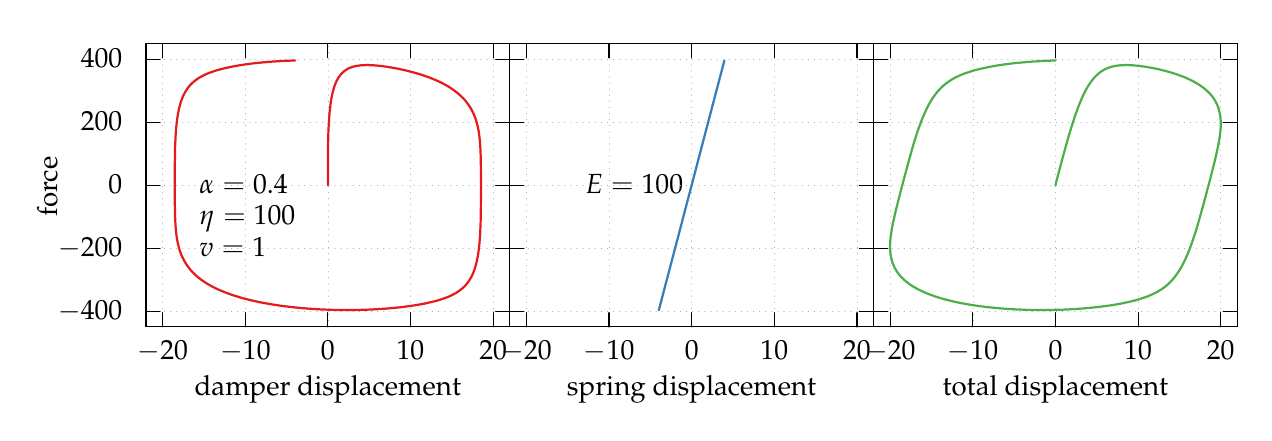
\begin{tikzpicture}[gnuplot]
%% generated with GNUPLOT 5.4p2 (Lua 5.4; terminal rev. Jun 2020, script rev. 114)
%% 11/05/21 19:38:29
\path (0.000,0.000) rectangle (14.000,4.000);
\gpcolor{color=gp lt color axes}
\gpsetlinetype{gp lt axes}
\gpsetdashtype{gp dt axes}
\gpsetlinewidth{0.50}
\draw[gp path] (0.140,0.400)--(4.759,0.400);
\gpcolor{color=gp lt color border}
\gpsetlinetype{gp lt border}
\gpsetdashtype{gp dt solid}
\gpsetlinewidth{1.00}
\draw[gp path] (0.140,0.400)--(0.320,0.400);
\draw[gp path] (4.759,0.400)--(4.579,0.400);
\node[gp node right] at (-0.044,0.400) {$-400$};
\gpcolor{color=gp lt color axes}
\gpsetlinetype{gp lt axes}
\gpsetdashtype{gp dt axes}
\gpsetlinewidth{0.50}
\draw[gp path] (0.140,1.200)--(4.759,1.200);
\gpcolor{color=gp lt color border}
\gpsetlinetype{gp lt border}
\gpsetdashtype{gp dt solid}
\gpsetlinewidth{1.00}
\draw[gp path] (0.140,1.200)--(0.320,1.200);
\draw[gp path] (4.759,1.200)--(4.579,1.200);
\node[gp node right] at (-0.044,1.200) {$-200$};
\gpcolor{color=gp lt color axes}
\gpsetlinetype{gp lt axes}
\gpsetdashtype{gp dt axes}
\gpsetlinewidth{0.50}
\draw[gp path] (0.140,2.000)--(4.759,2.000);
\gpcolor{color=gp lt color border}
\gpsetlinetype{gp lt border}
\gpsetdashtype{gp dt solid}
\gpsetlinewidth{1.00}
\draw[gp path] (0.140,2.000)--(0.320,2.000);
\draw[gp path] (4.759,2.000)--(4.579,2.000);
\node[gp node right] at (-0.044,2.000) {$0$};
\gpcolor{color=gp lt color axes}
\gpsetlinetype{gp lt axes}
\gpsetdashtype{gp dt axes}
\gpsetlinewidth{0.50}
\draw[gp path] (0.140,2.799)--(4.759,2.799);
\gpcolor{color=gp lt color border}
\gpsetlinetype{gp lt border}
\gpsetdashtype{gp dt solid}
\gpsetlinewidth{1.00}
\draw[gp path] (0.140,2.799)--(0.320,2.799);
\draw[gp path] (4.759,2.799)--(4.579,2.799);
\node[gp node right] at (-0.044,2.799) {$200$};
\gpcolor{color=gp lt color axes}
\gpsetlinetype{gp lt axes}
\gpsetdashtype{gp dt axes}
\gpsetlinewidth{0.50}
\draw[gp path] (0.140,3.599)--(4.759,3.599);
\gpcolor{color=gp lt color border}
\gpsetlinetype{gp lt border}
\gpsetdashtype{gp dt solid}
\gpsetlinewidth{1.00}
\draw[gp path] (0.140,3.599)--(0.320,3.599);
\draw[gp path] (4.759,3.599)--(4.579,3.599);
\node[gp node right] at (-0.044,3.599) {$400$};
\gpcolor{color=gp lt color axes}
\gpsetlinetype{gp lt axes}
\gpsetdashtype{gp dt axes}
\gpsetlinewidth{0.50}
\draw[gp path] (0.350,0.200)--(0.350,0.380)--(0.350,3.799);
\gpcolor{color=gp lt color border}
\gpsetlinetype{gp lt border}
\gpsetdashtype{gp dt solid}
\gpsetlinewidth{1.00}
\draw[gp path] (0.350,0.200)--(0.350,0.380);
\draw[gp path] (0.350,3.799)--(0.350,3.619);
\node[gp node center] at (0.350,-0.108) {$-20$};
\gpcolor{color=gp lt color axes}
\gpsetlinetype{gp lt axes}
\gpsetdashtype{gp dt axes}
\gpsetlinewidth{0.50}
\draw[gp path] (1.400,0.200)--(1.400,3.799);
\gpcolor{color=gp lt color border}
\gpsetlinetype{gp lt border}
\gpsetdashtype{gp dt solid}
\gpsetlinewidth{1.00}
\draw[gp path] (1.400,0.200)--(1.400,0.380);
\draw[gp path] (1.400,3.799)--(1.400,3.619);
\node[gp node center] at (1.400,-0.108) {$-10$};
\gpcolor{color=gp lt color axes}
\gpsetlinetype{gp lt axes}
\gpsetdashtype{gp dt axes}
\gpsetlinewidth{0.50}
\draw[gp path] (2.450,0.200)--(2.450,3.799);
\gpcolor{color=gp lt color border}
\gpsetlinetype{gp lt border}
\gpsetdashtype{gp dt solid}
\gpsetlinewidth{1.00}
\draw[gp path] (2.450,0.200)--(2.450,0.380);
\draw[gp path] (2.450,3.799)--(2.450,3.619);
\node[gp node center] at (2.450,-0.108) {$0$};
\gpcolor{color=gp lt color axes}
\gpsetlinetype{gp lt axes}
\gpsetdashtype{gp dt axes}
\gpsetlinewidth{0.50}
\draw[gp path] (3.499,0.200)--(3.499,3.799);
\gpcolor{color=gp lt color border}
\gpsetlinetype{gp lt border}
\gpsetdashtype{gp dt solid}
\gpsetlinewidth{1.00}
\draw[gp path] (3.499,0.200)--(3.499,0.380);
\draw[gp path] (3.499,3.799)--(3.499,3.619);
\node[gp node center] at (3.499,-0.108) {$10$};
\gpcolor{color=gp lt color axes}
\gpsetlinetype{gp lt axes}
\gpsetdashtype{gp dt axes}
\gpsetlinewidth{0.50}
\draw[gp path] (4.549,0.200)--(4.549,3.799);
\gpcolor{color=gp lt color border}
\gpsetlinetype{gp lt border}
\gpsetdashtype{gp dt solid}
\gpsetlinewidth{1.00}
\draw[gp path] (4.549,0.200)--(4.549,0.380);
\draw[gp path] (4.549,3.799)--(4.549,3.619);
\node[gp node center] at (4.549,-0.108) {$20$};
\draw[gp path] (0.140,3.799)--(0.140,0.200)--(4.759,0.200)--(4.759,3.799)--cycle;
\node[gp node left] at (0.700,2.000) {$\alpha=0.4$};
\node[gp node left] at (0.700,1.600) {$\eta=100$};
\node[gp node left] at (0.700,1.200) {$v=1$};
\node[gp node left] at (5.600,2.000) {$E=100$};
\node[gp node center,rotate=-270] at (-1.072,1.999) {force};
\node[gp node center] at (2.449,-0.569) {damper displacement};
\gpcolor{rgb color={0.894,0.102,0.110}}
\gpsetlinewidth{2.00}
\draw[gp path] (2.450,2.000)--(2.450,2.125)--(2.450,2.249)--(2.451,2.372)--(2.452,2.492)%
  --(2.454,2.608)--(2.458,2.719)--(2.464,2.823)--(2.471,2.920)--(2.481,3.008)--(2.492,3.088)%
  --(2.506,3.159)--(2.522,3.221)--(2.540,3.275)--(2.560,3.322)--(2.582,3.362)--(2.605,3.395)%
  --(2.630,3.423)--(2.655,3.446)--(2.682,3.466)--(2.709,3.481)--(2.737,3.493)--(2.766,3.503)%
  --(2.795,3.511)--(2.824,3.516)--(2.854,3.520)--(2.883,3.523)--(2.913,3.524)--(2.943,3.525)%
  --(2.973,3.525)--(3.003,3.523)--(3.032,3.522)--(3.062,3.519)--(3.091,3.517)--(3.121,3.513)%
  --(3.150,3.510)--(3.179,3.506)--(3.208,3.502)--(3.236,3.497)--(3.265,3.492)--(3.293,3.487)%
  --(3.321,3.482)--(3.349,3.477)--(3.376,3.471)--(3.403,3.465)--(3.430,3.459)--(3.456,3.453)%
  --(3.483,3.446)--(3.509,3.439)--(3.534,3.432)--(3.560,3.425)--(3.585,3.418)--(3.610,3.411)%
  --(3.634,3.403)--(3.658,3.395)--(3.682,3.387)--(3.705,3.379)--(3.728,3.371)--(3.751,3.362)%
  --(3.773,3.353)--(3.795,3.344)--(3.817,3.335)--(3.838,3.326)--(3.859,3.316)--(3.879,3.306)%
  --(3.899,3.296)--(3.919,3.286)--(3.938,3.276)--(3.957,3.265)--(3.976,3.254)--(3.994,3.243)%
  --(4.011,3.232)--(4.029,3.220)--(4.046,3.209)--(4.062,3.197)--(4.078,3.184)--(4.094,3.172)%
  --(4.109,3.159)--(4.124,3.146)--(4.138,3.133)--(4.152,3.119)--(4.166,3.106)--(4.179,3.092)%
  --(4.192,3.077)--(4.204,3.062)--(4.216,3.047)--(4.227,3.032)--(4.238,3.017)--(4.249,3.001)%
  --(4.259,2.984)--(4.269,2.968)--(4.278,2.951)--(4.287,2.933)--(4.296,2.916)--(4.304,2.897)%
  --(4.312,2.879)--(4.319,2.860)--(4.326,2.840)--(4.333,2.820)--(4.339,2.800)--(4.344,2.779)%
  --(4.350,2.757)--(4.355,2.735)--(4.359,2.713)--(4.364,2.690)--(4.368,2.666)--(4.371,2.641)%
  --(4.375,2.616)--(4.377,2.590)--(4.380,2.563)--(4.382,2.536)--(4.384,2.507)--(4.386,2.478)%
  --(4.388,2.448)--(4.389,2.416)--(4.390,2.384)--(4.391,2.350)--(4.392,2.315)--(4.392,2.279)%
  --(4.393,2.240)--(4.393,2.201)--(4.394,2.160)--(4.394,2.117)--(4.394,2.073)--(4.394,2.027)%
  --(4.394,1.980)--(4.394,1.931)--(4.394,1.881)--(4.394,1.829)--(4.393,1.777)--(4.393,1.723)%
  --(4.392,1.667)--(4.391,1.611)--(4.390,1.554)--(4.389,1.497)--(4.386,1.440)--(4.384,1.384)%
  --(4.380,1.329)--(4.376,1.276)--(4.371,1.223)--(4.365,1.173)--(4.358,1.125)--(4.350,1.079)%
  --(4.341,1.035)--(4.331,0.994)--(4.320,0.955)--(4.308,0.919)--(4.295,0.885)--(4.281,0.854)%
  --(4.266,0.824)--(4.250,0.797)--(4.233,0.772)--(4.215,0.749)--(4.197,0.727)--(4.177,0.707)%
  --(4.157,0.689)--(4.136,0.672)--(4.115,0.656)--(4.093,0.641)--(4.070,0.627)--(4.047,0.615)%
  --(4.023,0.603)--(3.999,0.591)--(3.975,0.581)--(3.950,0.571)--(3.924,0.562)--(3.898,0.553)%
  --(3.872,0.544)--(3.845,0.536)--(3.818,0.529)--(3.791,0.522)--(3.763,0.515)--(3.735,0.509)%
  --(3.707,0.502)--(3.678,0.496)--(3.649,0.491)--(3.620,0.485)--(3.590,0.480)--(3.561,0.475)%
  --(3.531,0.471)--(3.501,0.466)--(3.470,0.462)--(3.440,0.458)--(3.409,0.454)--(3.378,0.450)%
  --(3.347,0.447)--(3.316,0.444)--(3.285,0.441)--(3.253,0.438)--(3.221,0.435)--(3.189,0.432)%
  --(3.157,0.430)--(3.125,0.428)--(3.093,0.426)--(3.061,0.424)--(3.028,0.422)--(2.996,0.420)%
  --(2.963,0.419)--(2.931,0.418)--(2.898,0.417)--(2.865,0.416)--(2.832,0.415)--(2.800,0.415)%
  --(2.767,0.414)--(2.734,0.414)--(2.701,0.414)--(2.668,0.414)--(2.635,0.414)--(2.602,0.414)%
  --(2.570,0.415)--(2.537,0.416)--(2.504,0.416)--(2.471,0.417)--(2.439,0.419)--(2.406,0.420)%
  --(2.374,0.421)--(2.341,0.423)--(2.309,0.425)--(2.277,0.427)--(2.244,0.429)--(2.212,0.431)%
  --(2.181,0.434)--(2.149,0.436)--(2.117,0.439)--(2.086,0.442)--(2.054,0.445)--(2.023,0.448)%
  --(1.992,0.451)--(1.961,0.455)--(1.930,0.459)--(1.900,0.462)--(1.870,0.466)--(1.839,0.470)%
  --(1.810,0.475)--(1.780,0.479)--(1.750,0.484)--(1.721,0.489)--(1.692,0.494)--(1.663,0.499)%
  --(1.635,0.504)--(1.607,0.509)--(1.579,0.515)--(1.551,0.521)--(1.523,0.527)--(1.496,0.533)%
  --(1.469,0.539)--(1.443,0.546)--(1.416,0.552)--(1.390,0.559)--(1.365,0.566)--(1.339,0.573)%
  --(1.314,0.581)--(1.290,0.588)--(1.265,0.596)--(1.241,0.604)--(1.217,0.612)--(1.194,0.620)%
  --(1.171,0.628)--(1.148,0.637)--(1.126,0.646)--(1.104,0.655)--(1.082,0.664)--(1.061,0.673)%
  --(1.040,0.683)--(1.020,0.693)--(1.000,0.703)--(0.980,0.713)--(0.961,0.723)--(0.942,0.734)%
  --(0.923,0.745)--(0.905,0.756)--(0.888,0.767)--(0.870,0.779)--(0.853,0.790)--(0.837,0.802)%
  --(0.821,0.815)--(0.805,0.827)--(0.790,0.840)--(0.775,0.853)--(0.761,0.866)--(0.747,0.880)%
  --(0.733,0.893)--(0.720,0.907)--(0.707,0.922)--(0.695,0.937)--(0.683,0.952)--(0.672,0.967)%
  --(0.661,0.982)--(0.650,0.998)--(0.640,1.015)--(0.630,1.031)--(0.621,1.048)--(0.612,1.066)%
  --(0.603,1.083)--(0.595,1.102)--(0.587,1.120)--(0.580,1.139)--(0.573,1.159)--(0.566,1.179)%
  --(0.560,1.199)--(0.555,1.220)--(0.549,1.242)--(0.544,1.264)--(0.540,1.286)--(0.535,1.309)%
  --(0.531,1.333)--(0.528,1.358)--(0.524,1.383)--(0.522,1.409)--(0.519,1.436)--(0.517,1.463)%
  --(0.515,1.492)--(0.513,1.521)--(0.511,1.551)--(0.510,1.583)--(0.509,1.615)--(0.508,1.649)%
  --(0.507,1.684)--(0.507,1.720)--(0.506,1.759)--(0.506,1.798)--(0.505,1.839)--(0.505,1.882)%
  --(0.505,1.926)--(0.505,1.972)--(0.505,2.019)--(0.505,2.068)--(0.505,2.118)--(0.505,2.170)%
  --(0.506,2.222)--(0.506,2.276)--(0.507,2.332)--(0.508,2.388)--(0.509,2.445)--(0.510,2.502)%
  --(0.513,2.559)--(0.515,2.615)--(0.519,2.670)--(0.523,2.723)--(0.528,2.776)--(0.534,2.826)%
  --(0.541,2.874)--(0.549,2.920)--(0.558,2.964)--(0.568,3.005)--(0.579,3.044)--(0.591,3.080)%
  --(0.604,3.114)--(0.618,3.145)--(0.633,3.175)--(0.649,3.202)--(0.666,3.227)--(0.684,3.250)%
  --(0.702,3.272)--(0.722,3.292)--(0.742,3.310)--(0.763,3.327)--(0.784,3.343)--(0.806,3.358)%
  --(0.829,3.372)--(0.852,3.384)--(0.876,3.396)--(0.900,3.408)--(0.924,3.418)--(0.949,3.428)%
  --(0.975,3.437)--(1.001,3.446)--(1.027,3.455)--(1.054,3.463)--(1.081,3.470)--(1.108,3.477)%
  --(1.136,3.484)--(1.164,3.490)--(1.192,3.497)--(1.221,3.503)--(1.250,3.508)--(1.279,3.514)%
  --(1.309,3.519)--(1.338,3.524)--(1.368,3.528)--(1.398,3.533)--(1.429,3.537)--(1.459,3.541)%
  --(1.490,3.545)--(1.521,3.549)--(1.552,3.552)--(1.583,3.555)--(1.614,3.558)--(1.646,3.561)%
  --(1.678,3.564)--(1.710,3.567)--(1.742,3.569)--(1.774,3.571)--(1.806,3.573)--(1.838,3.575)%
  --(1.871,3.577)--(1.903,3.579)--(1.936,3.580)--(1.968,3.581)--(2.001,3.582)--(2.034,3.583);
\gpcolor{color=gp lt color border}
\gpsetlinewidth{1.00}
\draw[gp path] (0.140,3.799)--(0.140,0.200)--(4.759,0.200)--(4.759,3.799)--cycle;
%% coordinates of the plot area
\gpdefrectangularnode{gp plot 1}{\pgfpoint{0.140cm}{0.200cm}}{\pgfpoint{4.759cm}{3.799cm}}
\gpcolor{color=gp lt color axes}
\gpsetlinetype{gp lt axes}
\gpsetdashtype{gp dt axes}
\gpsetlinewidth{0.50}
\draw[gp path] (4.760,0.400)--(9.379,0.400);
\gpcolor{color=gp lt color border}
\gpsetlinetype{gp lt border}
\gpsetdashtype{gp dt solid}
\gpsetlinewidth{1.00}
\draw[gp path] (4.760,0.400)--(4.940,0.400);
\draw[gp path] (9.379,0.400)--(9.199,0.400);
\gpcolor{color=gp lt color axes}
\gpsetlinetype{gp lt axes}
\gpsetdashtype{gp dt axes}
\gpsetlinewidth{0.50}
\draw[gp path] (4.760,1.200)--(9.379,1.200);
\gpcolor{color=gp lt color border}
\gpsetlinetype{gp lt border}
\gpsetdashtype{gp dt solid}
\gpsetlinewidth{1.00}
\draw[gp path] (4.760,1.200)--(4.940,1.200);
\draw[gp path] (9.379,1.200)--(9.199,1.200);
\gpcolor{color=gp lt color axes}
\gpsetlinetype{gp lt axes}
\gpsetdashtype{gp dt axes}
\gpsetlinewidth{0.50}
\draw[gp path] (4.760,2.000)--(9.379,2.000);
\gpcolor{color=gp lt color border}
\gpsetlinetype{gp lt border}
\gpsetdashtype{gp dt solid}
\gpsetlinewidth{1.00}
\draw[gp path] (4.760,2.000)--(4.940,2.000);
\draw[gp path] (9.379,2.000)--(9.199,2.000);
\gpcolor{color=gp lt color axes}
\gpsetlinetype{gp lt axes}
\gpsetdashtype{gp dt axes}
\gpsetlinewidth{0.50}
\draw[gp path] (4.760,2.799)--(9.379,2.799);
\gpcolor{color=gp lt color border}
\gpsetlinetype{gp lt border}
\gpsetdashtype{gp dt solid}
\gpsetlinewidth{1.00}
\draw[gp path] (4.760,2.799)--(4.940,2.799);
\draw[gp path] (9.379,2.799)--(9.199,2.799);
\gpcolor{color=gp lt color axes}
\gpsetlinetype{gp lt axes}
\gpsetdashtype{gp dt axes}
\gpsetlinewidth{0.50}
\draw[gp path] (4.760,3.599)--(9.379,3.599);
\gpcolor{color=gp lt color border}
\gpsetlinetype{gp lt border}
\gpsetdashtype{gp dt solid}
\gpsetlinewidth{1.00}
\draw[gp path] (4.760,3.599)--(4.940,3.599);
\draw[gp path] (9.379,3.599)--(9.199,3.599);
\gpcolor{color=gp lt color axes}
\gpsetlinetype{gp lt axes}
\gpsetdashtype{gp dt axes}
\gpsetlinewidth{0.50}
\draw[gp path] (4.970,0.200)--(4.970,3.799);
\gpcolor{color=gp lt color border}
\gpsetlinetype{gp lt border}
\gpsetdashtype{gp dt solid}
\gpsetlinewidth{1.00}
\draw[gp path] (4.970,0.200)--(4.970,0.380);
\draw[gp path] (4.970,3.799)--(4.970,3.619);
\node[gp node center] at (4.970,-0.108) {$-20$};
\gpcolor{color=gp lt color axes}
\gpsetlinetype{gp lt axes}
\gpsetdashtype{gp dt axes}
\gpsetlinewidth{0.50}
\draw[gp path] (6.020,0.200)--(6.020,3.799);
\gpcolor{color=gp lt color border}
\gpsetlinetype{gp lt border}
\gpsetdashtype{gp dt solid}
\gpsetlinewidth{1.00}
\draw[gp path] (6.020,0.200)--(6.020,0.380);
\draw[gp path] (6.020,3.799)--(6.020,3.619);
\node[gp node center] at (6.020,-0.108) {$-10$};
\gpcolor{color=gp lt color axes}
\gpsetlinetype{gp lt axes}
\gpsetdashtype{gp dt axes}
\gpsetlinewidth{0.50}
\draw[gp path] (7.070,0.200)--(7.070,3.799);
\gpcolor{color=gp lt color border}
\gpsetlinetype{gp lt border}
\gpsetdashtype{gp dt solid}
\gpsetlinewidth{1.00}
\draw[gp path] (7.070,0.200)--(7.070,0.380);
\draw[gp path] (7.070,3.799)--(7.070,3.619);
\node[gp node center] at (7.070,-0.108) {$0$};
\gpcolor{color=gp lt color axes}
\gpsetlinetype{gp lt axes}
\gpsetdashtype{gp dt axes}
\gpsetlinewidth{0.50}
\draw[gp path] (8.119,0.200)--(8.119,3.799);
\gpcolor{color=gp lt color border}
\gpsetlinetype{gp lt border}
\gpsetdashtype{gp dt solid}
\gpsetlinewidth{1.00}
\draw[gp path] (8.119,0.200)--(8.119,0.380);
\draw[gp path] (8.119,3.799)--(8.119,3.619);
\node[gp node center] at (8.119,-0.108) {$10$};
\gpcolor{color=gp lt color axes}
\gpsetlinetype{gp lt axes}
\gpsetdashtype{gp dt axes}
\gpsetlinewidth{0.50}
\draw[gp path] (9.169,0.200)--(9.169,0.380)--(9.169,3.799);
\gpcolor{color=gp lt color border}
\gpsetlinetype{gp lt border}
\gpsetdashtype{gp dt solid}
\gpsetlinewidth{1.00}
\draw[gp path] (9.169,0.200)--(9.169,0.380);
\draw[gp path] (9.169,3.799)--(9.169,3.619);
\node[gp node center] at (9.169,-0.108) {$20$};
\draw[gp path] (4.760,3.799)--(4.760,0.200)--(9.379,0.200)--(9.379,3.799)--cycle;
\node[gp node center] at (7.069,-0.569) {spring displacement};
\gpcolor{rgb color={0.216,0.494,0.722}}
\gpsetlinewidth{2.00}
\draw[gp path] (7.070,2.000)--(7.102,2.125)--(7.135,2.249)--(7.167,2.372)--(7.199,2.492)%
  --(7.229,2.608)--(7.258,2.719)--(7.286,2.823)--(7.311,2.920)--(7.334,3.008)--(7.355,3.088)%
  --(7.374,3.159)--(7.390,3.221)--(7.404,3.275)--(7.417,3.322)--(7.427,3.362)--(7.436,3.395)%
  --(7.443,3.423)--(7.449,3.446)--(7.454,3.466)--(7.458,3.481)--(7.462,3.493)--(7.464,3.503)%
  --(7.466,3.511)--(7.468,3.516)--(7.469,3.520)--(7.469,3.523)--(7.470,3.524)--(7.470,3.525)%
  --(7.470,3.523)--(7.469,3.522)--(7.468,3.519)--(7.468,3.517)--(7.467,3.513)--(7.466,3.510)%
  --(7.465,3.506)--(7.464,3.502)--(7.463,3.497)--(7.461,3.492)--(7.460,3.487)--(7.459,3.482)%
  --(7.457,3.477)--(7.456,3.471)--(7.454,3.465)--(7.453,3.459)--(7.451,3.453)--(7.449,3.446)%
  --(7.447,3.439)--(7.446,3.432)--(7.444,3.425)--(7.442,3.418)--(7.440,3.411)--(7.438,3.403)%
  --(7.436,3.395)--(7.434,3.387)--(7.432,3.379)--(7.429,3.371)--(7.427,3.362)--(7.425,3.353)%
  --(7.423,3.344)--(7.420,3.335)--(7.418,3.326)--(7.415,3.316)--(7.413,3.306)--(7.410,3.296)%
  --(7.407,3.286)--(7.405,3.276)--(7.402,3.265)--(7.399,3.254)--(7.396,3.243)--(7.393,3.232)%
  --(7.390,3.220)--(7.387,3.209)--(7.384,3.197)--(7.381,3.184)--(7.377,3.172)--(7.374,3.159)%
  --(7.371,3.146)--(7.367,3.133)--(7.363,3.119)--(7.360,3.106)--(7.356,3.092)--(7.352,3.077)%
  --(7.349,3.062)--(7.345,3.047)--(7.341,3.032)--(7.336,3.017)--(7.332,3.001)--(7.328,2.984)%
  --(7.324,2.968)--(7.319,2.951)--(7.315,2.933)--(7.310,2.916)--(7.305,2.897)--(7.300,2.879)%
  --(7.295,2.860)--(7.290,2.840)--(7.285,2.820)--(7.280,2.800)--(7.274,2.779)--(7.268,2.757)%
  --(7.263,2.735)--(7.257,2.713)--(7.251,2.690)--(7.244,2.666)--(7.238,2.641)--(7.231,2.616)%
  --(7.225,2.590)--(7.217,2.563)--(7.210,2.536)--(7.203,2.507)--(7.195,2.478)--(7.187,2.448)%
  --(7.179,2.416)--(7.170,2.384)--(7.162,2.350)--(7.152,2.315)--(7.143,2.279)--(7.133,2.240)%
  --(7.122,2.201)--(7.112,2.160)--(7.100,2.117)--(7.089,2.073)--(7.077,2.027)--(7.064,1.980)%
  --(7.052,1.931)--(7.038,1.881)--(7.025,1.829)--(7.011,1.777)--(6.997,1.723)--(6.982,1.667)%
  --(6.967,1.611)--(6.953,1.554)--(6.938,1.497)--(6.923,1.440)--(6.908,1.384)--(6.894,1.329)%
  --(6.879,1.276)--(6.866,1.223)--(6.853,1.173)--(6.840,1.125)--(6.828,1.079)--(6.816,1.035)%
  --(6.806,0.994)--(6.795,0.955)--(6.786,0.919)--(6.777,0.885)--(6.769,0.854)--(6.761,0.824)%
  --(6.754,0.797)--(6.747,0.772)--(6.741,0.749)--(6.735,0.727)--(6.730,0.707)--(6.725,0.689)%
  --(6.721,0.672)--(6.717,0.656)--(6.713,0.641)--(6.709,0.627)--(6.706,0.615)--(6.703,0.603)%
  --(6.700,0.591)--(6.697,0.581)--(6.694,0.571)--(6.692,0.562)--(6.690,0.553)--(6.688,0.544)%
  --(6.685,0.536)--(6.683,0.529)--(6.682,0.522)--(6.680,0.515)--(6.678,0.509)--(6.676,0.502)%
  --(6.675,0.496)--(6.673,0.491)--(6.672,0.485)--(6.671,0.480)--(6.669,0.475)--(6.668,0.471)%
  --(6.667,0.466)--(6.666,0.462)--(6.665,0.458)--(6.664,0.454)--(6.663,0.450)--(6.662,0.447)%
  --(6.661,0.444)--(6.660,0.441)--(6.659,0.438)--(6.659,0.435)--(6.658,0.432)--(6.657,0.430)%
  --(6.657,0.428)--(6.656,0.426)--(6.656,0.424)--(6.655,0.422)--(6.655,0.420)--(6.655,0.419)%
  --(6.654,0.418)--(6.654,0.417)--(6.654,0.416)--(6.654,0.415)--(6.653,0.415)--(6.653,0.414)%
  --(6.654,0.415)--(6.654,0.416)--(6.654,0.417)--(6.654,0.419)--(6.655,0.420)--(6.655,0.421)%
  --(6.656,0.423)--(6.656,0.425)--(6.657,0.427)--(6.657,0.429)--(6.658,0.431)--(6.658,0.434)%
  --(6.659,0.436)--(6.660,0.439)--(6.661,0.442)--(6.661,0.445)--(6.662,0.448)--(6.663,0.451)%
  --(6.664,0.455)--(6.665,0.459)--(6.666,0.462)--(6.667,0.466)--(6.668,0.470)--(6.669,0.475)%
  --(6.670,0.479)--(6.672,0.484)--(6.673,0.489)--(6.674,0.494)--(6.676,0.499)--(6.677,0.504)%
  --(6.678,0.509)--(6.680,0.515)--(6.681,0.521)--(6.683,0.527)--(6.685,0.533)--(6.686,0.539)%
  --(6.688,0.546)--(6.690,0.552)--(6.691,0.559)--(6.693,0.566)--(6.695,0.573)--(6.697,0.581)%
  --(6.699,0.588)--(6.701,0.596)--(6.703,0.604)--(6.705,0.612)--(6.707,0.620)--(6.710,0.628)%
  --(6.712,0.637)--(6.714,0.646)--(6.716,0.655)--(6.719,0.664)--(6.721,0.673)--(6.724,0.683)%
  --(6.726,0.693)--(6.729,0.703)--(6.732,0.713)--(6.734,0.723)--(6.737,0.734)--(6.740,0.745)%
  --(6.743,0.756)--(6.746,0.767)--(6.749,0.779)--(6.752,0.790)--(6.755,0.802)--(6.758,0.815)%
  --(6.762,0.827)--(6.765,0.840)--(6.768,0.853)--(6.772,0.866)--(6.776,0.880)--(6.779,0.893)%
  --(6.783,0.907)--(6.787,0.922)--(6.790,0.937)--(6.794,0.952)--(6.798,0.967)--(6.803,0.982)%
  --(6.807,0.998)--(6.811,1.015)--(6.815,1.031)--(6.820,1.048)--(6.824,1.066)--(6.829,1.083)%
  --(6.834,1.102)--(6.839,1.120)--(6.844,1.139)--(6.849,1.159)--(6.854,1.179)--(6.859,1.199)%
  --(6.865,1.220)--(6.871,1.242)--(6.876,1.264)--(6.882,1.286)--(6.888,1.309)--(6.895,1.333)%
  --(6.901,1.358)--(6.908,1.383)--(6.914,1.409)--(6.922,1.436)--(6.929,1.463)--(6.936,1.492)%
  --(6.944,1.521)--(6.952,1.551)--(6.960,1.583)--(6.969,1.615)--(6.977,1.649)--(6.987,1.684)%
  --(6.996,1.720)--(7.006,1.759)--(7.017,1.798)--(7.027,1.839)--(7.039,1.882)--(7.050,1.926)%
  --(7.062,1.972)--(7.075,2.019)--(7.087,2.068)--(7.101,2.118)--(7.114,2.170)--(7.128,2.222)%
  --(7.142,2.276)--(7.157,2.332)--(7.172,2.388)--(7.186,2.445)--(7.201,2.502)--(7.216,2.559)%
  --(7.231,2.615)--(7.245,2.670)--(7.260,2.723)--(7.273,2.776)--(7.286,2.826)--(7.299,2.874)%
  --(7.311,2.920)--(7.323,2.964)--(7.333,3.005)--(7.344,3.044)--(7.353,3.080)--(7.362,3.114)%
  --(7.370,3.145)--(7.378,3.175)--(7.385,3.202)--(7.392,3.227)--(7.398,3.250)--(7.404,3.272)%
  --(7.409,3.292)--(7.414,3.310)--(7.418,3.327)--(7.422,3.343)--(7.426,3.358)--(7.430,3.372)%
  --(7.433,3.384)--(7.436,3.396)--(7.439,3.408)--(7.442,3.418)--(7.445,3.428)--(7.447,3.437)%
  --(7.449,3.446)--(7.451,3.455)--(7.454,3.463)--(7.456,3.470)--(7.457,3.477)--(7.459,3.484)%
  --(7.461,3.490)--(7.463,3.497)--(7.464,3.503)--(7.466,3.508)--(7.467,3.514)--(7.468,3.519)%
  --(7.470,3.524)--(7.471,3.528)--(7.472,3.533)--(7.473,3.537)--(7.474,3.541)--(7.475,3.545)%
  --(7.476,3.549)--(7.477,3.552)--(7.478,3.555)--(7.479,3.558)--(7.480,3.561)--(7.480,3.564)%
  --(7.481,3.567)--(7.482,3.569)--(7.482,3.571)--(7.483,3.573)--(7.483,3.575)--(7.484,3.577)%
  --(7.484,3.579)--(7.484,3.580)--(7.485,3.581)--(7.485,3.582)--(7.485,3.583);
\gpcolor{color=gp lt color border}
\gpsetlinewidth{1.00}
\draw[gp path] (4.760,3.799)--(4.760,0.200)--(9.379,0.200)--(9.379,3.799)--cycle;
%% coordinates of the plot area
\gpdefrectangularnode{gp plot 2}{\pgfpoint{4.760cm}{0.200cm}}{\pgfpoint{9.379cm}{3.799cm}}
\gpcolor{color=gp lt color axes}
\gpsetlinetype{gp lt axes}
\gpsetdashtype{gp dt axes}
\gpsetlinewidth{0.50}
\draw[gp path] (9.380,0.400)--(13.999,0.400);
\gpcolor{color=gp lt color border}
\gpsetlinetype{gp lt border}
\gpsetdashtype{gp dt solid}
\gpsetlinewidth{1.00}
\draw[gp path] (9.380,0.400)--(9.560,0.400);
\draw[gp path] (13.999,0.400)--(13.819,0.400);
\gpcolor{color=gp lt color axes}
\gpsetlinetype{gp lt axes}
\gpsetdashtype{gp dt axes}
\gpsetlinewidth{0.50}
\draw[gp path] (9.380,1.200)--(13.999,1.200);
\gpcolor{color=gp lt color border}
\gpsetlinetype{gp lt border}
\gpsetdashtype{gp dt solid}
\gpsetlinewidth{1.00}
\draw[gp path] (9.380,1.200)--(9.560,1.200);
\draw[gp path] (13.999,1.200)--(13.819,1.200);
\gpcolor{color=gp lt color axes}
\gpsetlinetype{gp lt axes}
\gpsetdashtype{gp dt axes}
\gpsetlinewidth{0.50}
\draw[gp path] (9.380,2.000)--(13.999,2.000);
\gpcolor{color=gp lt color border}
\gpsetlinetype{gp lt border}
\gpsetdashtype{gp dt solid}
\gpsetlinewidth{1.00}
\draw[gp path] (9.380,2.000)--(9.560,2.000);
\draw[gp path] (13.999,2.000)--(13.819,2.000);
\gpcolor{color=gp lt color axes}
\gpsetlinetype{gp lt axes}
\gpsetdashtype{gp dt axes}
\gpsetlinewidth{0.50}
\draw[gp path] (9.380,2.799)--(13.999,2.799);
\gpcolor{color=gp lt color border}
\gpsetlinetype{gp lt border}
\gpsetdashtype{gp dt solid}
\gpsetlinewidth{1.00}
\draw[gp path] (9.380,2.799)--(9.560,2.799);
\draw[gp path] (13.999,2.799)--(13.819,2.799);
\gpcolor{color=gp lt color axes}
\gpsetlinetype{gp lt axes}
\gpsetdashtype{gp dt axes}
\gpsetlinewidth{0.50}
\draw[gp path] (9.380,3.599)--(13.999,3.599);
\gpcolor{color=gp lt color border}
\gpsetlinetype{gp lt border}
\gpsetdashtype{gp dt solid}
\gpsetlinewidth{1.00}
\draw[gp path] (9.380,3.599)--(9.560,3.599);
\draw[gp path] (13.999,3.599)--(13.819,3.599);
\gpcolor{color=gp lt color axes}
\gpsetlinetype{gp lt axes}
\gpsetdashtype{gp dt axes}
\gpsetlinewidth{0.50}
\draw[gp path] (9.590,0.200)--(9.590,3.799);
\gpcolor{color=gp lt color border}
\gpsetlinetype{gp lt border}
\gpsetdashtype{gp dt solid}
\gpsetlinewidth{1.00}
\draw[gp path] (9.590,0.200)--(9.590,0.380);
\draw[gp path] (9.590,3.799)--(9.590,3.619);
\node[gp node center] at (9.590,-0.108) {$-20$};
\gpcolor{color=gp lt color axes}
\gpsetlinetype{gp lt axes}
\gpsetdashtype{gp dt axes}
\gpsetlinewidth{0.50}
\draw[gp path] (10.640,0.200)--(10.640,3.799);
\gpcolor{color=gp lt color border}
\gpsetlinetype{gp lt border}
\gpsetdashtype{gp dt solid}
\gpsetlinewidth{1.00}
\draw[gp path] (10.640,0.200)--(10.640,0.380);
\draw[gp path] (10.640,3.799)--(10.640,3.619);
\node[gp node center] at (10.640,-0.108) {$-10$};
\gpcolor{color=gp lt color axes}
\gpsetlinetype{gp lt axes}
\gpsetdashtype{gp dt axes}
\gpsetlinewidth{0.50}
\draw[gp path] (11.690,0.200)--(11.690,3.799);
\gpcolor{color=gp lt color border}
\gpsetlinetype{gp lt border}
\gpsetdashtype{gp dt solid}
\gpsetlinewidth{1.00}
\draw[gp path] (11.690,0.200)--(11.690,0.380);
\draw[gp path] (11.690,3.799)--(11.690,3.619);
\node[gp node center] at (11.690,-0.108) {$0$};
\gpcolor{color=gp lt color axes}
\gpsetlinetype{gp lt axes}
\gpsetdashtype{gp dt axes}
\gpsetlinewidth{0.50}
\draw[gp path] (12.739,0.200)--(12.739,3.799);
\gpcolor{color=gp lt color border}
\gpsetlinetype{gp lt border}
\gpsetdashtype{gp dt solid}
\gpsetlinewidth{1.00}
\draw[gp path] (12.739,0.200)--(12.739,0.380);
\draw[gp path] (12.739,3.799)--(12.739,3.619);
\node[gp node center] at (12.739,-0.108) {$10$};
\gpcolor{color=gp lt color axes}
\gpsetlinetype{gp lt axes}
\gpsetdashtype{gp dt axes}
\gpsetlinewidth{0.50}
\draw[gp path] (13.789,0.200)--(13.789,0.380)--(13.789,3.799);
\gpcolor{color=gp lt color border}
\gpsetlinetype{gp lt border}
\gpsetdashtype{gp dt solid}
\gpsetlinewidth{1.00}
\draw[gp path] (13.789,0.200)--(13.789,0.380);
\draw[gp path] (13.789,3.799)--(13.789,3.619);
\node[gp node center] at (13.789,-0.108) {$20$};
\draw[gp path] (9.380,3.799)--(9.380,0.200)--(13.999,0.200)--(13.999,3.799)--cycle;
\node[gp node center] at (11.689,-0.569) {total displacement};
\gpcolor{rgb color={0.302,0.686,0.290}}
\gpsetlinewidth{2.00}
\draw[gp path] (11.690,2.000)--(11.722,2.125)--(11.755,2.249)--(11.788,2.372)--(11.821,2.492)%
  --(11.854,2.608)--(11.887,2.719)--(11.920,2.823)--(11.953,2.920)--(11.985,3.008)--(12.018,3.088)%
  --(12.050,3.159)--(12.083,3.221)--(12.115,3.275)--(12.148,3.322)--(12.180,3.362)--(12.212,3.395)%
  --(12.244,3.423)--(12.275,3.446)--(12.307,3.466)--(12.338,3.481)--(12.370,3.493)--(12.401,3.503)%
  --(12.432,3.511)--(12.462,3.516)--(12.493,3.520)--(12.523,3.523)--(12.553,3.524)--(12.583,3.525)%
  --(12.613,3.525)--(12.643,3.523)--(12.672,3.522)--(12.701,3.519)--(12.730,3.517)--(12.758,3.513)%
  --(12.787,3.510)--(12.814,3.506)--(12.842,3.502)--(12.870,3.497)--(12.897,3.492)--(12.924,3.487)%
  --(12.950,3.482)--(12.976,3.477)--(13.002,3.471)--(13.028,3.465)--(13.053,3.459)--(13.078,3.453)%
  --(13.103,3.446)--(13.127,3.439)--(13.151,3.432)--(13.174,3.425)--(13.197,3.418)--(13.220,3.411)%
  --(13.242,3.403)--(13.264,3.395)--(13.286,3.387)--(13.307,3.379)--(13.328,3.371)--(13.348,3.362)%
  --(13.368,3.353)--(13.388,3.344)--(13.407,3.335)--(13.426,3.326)--(13.444,3.316)--(13.462,3.306)%
  --(13.480,3.296)--(13.497,3.286)--(13.513,3.276)--(13.529,3.265)--(13.545,3.254)--(13.560,3.243)%
  --(13.575,3.232)--(13.589,3.220)--(13.603,3.209)--(13.616,3.197)--(13.629,3.184)--(13.642,3.172)%
  --(13.654,3.159)--(13.665,3.146)--(13.676,3.133)--(13.686,3.119)--(13.696,3.106)--(13.706,3.092)%
  --(13.715,3.077)--(13.723,3.062)--(13.731,3.047)--(13.738,3.032)--(13.745,3.017)--(13.752,3.001)%
  --(13.758,2.984)--(13.763,2.968)--(13.768,2.951)--(13.772,2.933)--(13.776,2.916)--(13.780,2.897)%
  --(13.783,2.879)--(13.785,2.860)--(13.787,2.840)--(13.788,2.820)--(13.789,2.800)--(13.789,2.779)%
  --(13.789,2.757)--(13.788,2.735)--(13.787,2.713)--(13.785,2.690)--(13.783,2.666)--(13.780,2.641)%
  --(13.776,2.616)--(13.772,2.590)--(13.768,2.563)--(13.763,2.536)--(13.758,2.507)--(13.752,2.478)%
  --(13.745,2.448)--(13.738,2.416)--(13.731,2.384)--(13.723,2.350)--(13.715,2.315)--(13.706,2.279)%
  --(13.696,2.240)--(13.686,2.201)--(13.676,2.160)--(13.665,2.117)--(13.654,2.073)--(13.642,2.027)%
  --(13.629,1.980)--(13.616,1.931)--(13.603,1.881)--(13.589,1.829)--(13.575,1.777)--(13.560,1.723)%
  --(13.545,1.667)--(13.529,1.611)--(13.513,1.554)--(13.497,1.497)--(13.480,1.440)--(13.462,1.384)%
  --(13.444,1.329)--(13.426,1.276)--(13.407,1.223)--(13.388,1.173)--(13.368,1.125)--(13.348,1.079)%
  --(13.328,1.035)--(13.307,0.994)--(13.286,0.955)--(13.264,0.919)--(13.242,0.885)--(13.220,0.854)%
  --(13.197,0.824)--(13.174,0.797)--(13.151,0.772)--(13.127,0.749)--(13.103,0.727)--(13.078,0.707)%
  --(13.053,0.689)--(13.028,0.672)--(13.002,0.656)--(12.976,0.641)--(12.950,0.627)--(12.924,0.615)%
  --(12.897,0.603)--(12.870,0.591)--(12.842,0.581)--(12.814,0.571)--(12.787,0.562)--(12.758,0.553)%
  --(12.730,0.544)--(12.701,0.536)--(12.672,0.529)--(12.643,0.522)--(12.613,0.515)--(12.583,0.509)%
  --(12.553,0.502)--(12.523,0.496)--(12.493,0.491)--(12.462,0.485)--(12.432,0.480)--(12.401,0.475)%
  --(12.370,0.471)--(12.338,0.466)--(12.307,0.462)--(12.275,0.458)--(12.244,0.454)--(12.212,0.450)%
  --(12.180,0.447)--(12.148,0.444)--(12.115,0.441)--(12.083,0.438)--(12.050,0.435)--(12.018,0.432)%
  --(11.985,0.430)--(11.953,0.428)--(11.920,0.426)--(11.887,0.424)--(11.854,0.422)--(11.821,0.420)%
  --(11.788,0.419)--(11.755,0.418)--(11.722,0.417)--(11.690,0.416)--(11.657,0.415)--(11.624,0.415)%
  --(11.591,0.414)--(11.558,0.414)--(11.525,0.414)--(11.492,0.414)--(11.459,0.414)--(11.426,0.414)%
  --(11.394,0.415)--(11.361,0.416)--(11.329,0.416)--(11.296,0.417)--(11.264,0.419)--(11.231,0.420)%
  --(11.199,0.421)--(11.167,0.423)--(11.135,0.425)--(11.104,0.427)--(11.072,0.429)--(11.041,0.431)%
  --(11.009,0.434)--(10.978,0.436)--(10.947,0.439)--(10.917,0.442)--(10.886,0.445)--(10.856,0.448)%
  --(10.826,0.451)--(10.796,0.455)--(10.766,0.459)--(10.736,0.462)--(10.707,0.466)--(10.678,0.470)%
  --(10.649,0.475)--(10.621,0.479)--(10.592,0.484)--(10.565,0.489)--(10.537,0.494)--(10.509,0.499)%
  --(10.482,0.504)--(10.455,0.509)--(10.429,0.515)--(10.403,0.521)--(10.377,0.527)--(10.351,0.533)%
  --(10.326,0.539)--(10.301,0.546)--(10.276,0.552)--(10.252,0.559)--(10.228,0.566)--(10.205,0.573)%
  --(10.182,0.581)--(10.159,0.588)--(10.137,0.596)--(10.115,0.604)--(10.093,0.612)--(10.072,0.620)%
  --(10.051,0.628)--(10.031,0.637)--(10.011,0.646)--(9.991,0.655)--(9.972,0.664)--(9.953,0.673)%
  --(9.935,0.683)--(9.917,0.693)--(9.899,0.703)--(9.882,0.713)--(9.866,0.723)--(9.850,0.734)%
  --(9.834,0.745)--(9.819,0.756)--(9.804,0.767)--(9.790,0.779)--(9.776,0.790)--(9.763,0.802)%
  --(9.750,0.815)--(9.737,0.827)--(9.725,0.840)--(9.714,0.853)--(9.703,0.866)--(9.693,0.880)%
  --(9.683,0.893)--(9.673,0.907)--(9.664,0.922)--(9.656,0.937)--(9.648,0.952)--(9.641,0.967)%
  --(9.634,0.982)--(9.627,0.998)--(9.621,1.015)--(9.616,1.031)--(9.611,1.048)--(9.607,1.066)%
  --(9.603,1.083)--(9.599,1.102)--(9.596,1.120)--(9.594,1.139)--(9.592,1.159)--(9.591,1.179)%
  --(9.590,1.199)--(9.590,1.220)--(9.590,1.242)--(9.591,1.264)--(9.592,1.286)--(9.594,1.309)%
  --(9.596,1.333)--(9.599,1.358)--(9.603,1.383)--(9.607,1.409)--(9.611,1.436)--(9.616,1.463)%
  --(9.621,1.492)--(9.627,1.521)--(9.634,1.551)--(9.641,1.583)--(9.648,1.615)--(9.656,1.649)%
  --(9.664,1.684)--(9.673,1.720)--(9.683,1.759)--(9.693,1.798)--(9.703,1.839)--(9.714,1.882)%
  --(9.725,1.926)--(9.737,1.972)--(9.750,2.019)--(9.763,2.068)--(9.776,2.118)--(9.790,2.170)%
  --(9.804,2.222)--(9.819,2.276)--(9.834,2.332)--(9.850,2.388)--(9.866,2.445)--(9.882,2.502)%
  --(9.899,2.559)--(9.917,2.615)--(9.935,2.670)--(9.953,2.723)--(9.972,2.776)--(9.991,2.826)%
  --(10.011,2.874)--(10.031,2.920)--(10.051,2.964)--(10.072,3.005)--(10.093,3.044)--(10.115,3.080)%
  --(10.137,3.114)--(10.159,3.145)--(10.182,3.175)--(10.205,3.202)--(10.228,3.227)--(10.252,3.250)%
  --(10.276,3.272)--(10.301,3.292)--(10.326,3.310)--(10.351,3.327)--(10.377,3.343)--(10.403,3.358)%
  --(10.429,3.372)--(10.455,3.384)--(10.482,3.396)--(10.509,3.408)--(10.537,3.418)--(10.565,3.428)%
  --(10.592,3.437)--(10.621,3.446)--(10.649,3.455)--(10.678,3.463)--(10.707,3.470)--(10.736,3.477)%
  --(10.766,3.484)--(10.796,3.490)--(10.826,3.497)--(10.856,3.503)--(10.886,3.508)--(10.917,3.514)%
  --(10.947,3.519)--(10.978,3.524)--(11.009,3.528)--(11.041,3.533)--(11.072,3.537)--(11.104,3.541)%
  --(11.135,3.545)--(11.167,3.549)--(11.199,3.552)--(11.231,3.555)--(11.264,3.558)--(11.296,3.561)%
  --(11.329,3.564)--(11.361,3.567)--(11.394,3.569)--(11.426,3.571)--(11.459,3.573)--(11.492,3.575)%
  --(11.525,3.577)--(11.558,3.579)--(11.591,3.580)--(11.624,3.581)--(11.657,3.582)--(11.690,3.583);
\gpcolor{color=gp lt color border}
\gpsetlinewidth{1.00}
\draw[gp path] (9.380,3.799)--(9.380,0.200)--(13.999,0.200)--(13.999,3.799)--cycle;
%% coordinates of the plot area
\gpdefrectangularnode{gp plot 3}{\pgfpoint{9.380cm}{0.200cm}}{\pgfpoint{13.999cm}{3.799cm}}
\end{tikzpicture}
%% gnuplot variables

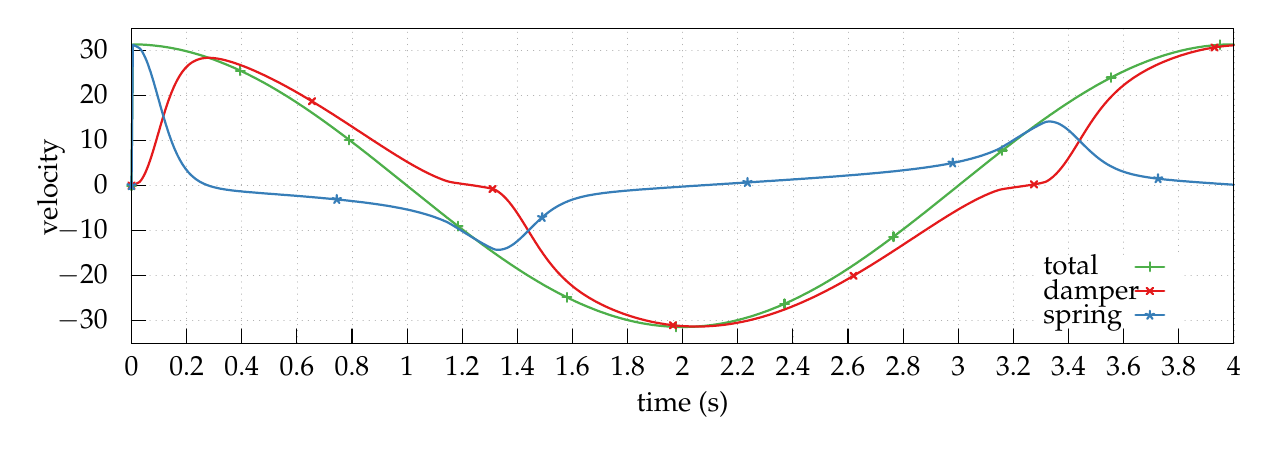
\begin{tikzpicture}[gnuplot]
%% generated with GNUPLOT 5.4p2 (Lua 5.4; terminal rev. Jun 2020, script rev. 114)
%% 11/09/21 03:15:53
\path (0.000,0.000) rectangle (14.000,4.000);
\gpcolor{color=gp lt color axes}
\gpsetlinetype{gp lt axes}
\gpsetdashtype{gp dt axes}
\gpsetlinewidth{0.50}
\draw[gp path] (0.000,0.286)--(11.463,0.286);
\draw[gp path] (13.299,0.286)--(13.999,0.286);
\gpcolor{color=gp lt color border}
\gpsetlinetype{gp lt border}
\gpsetdashtype{gp dt solid}
\gpsetlinewidth{1.00}
\draw[gp path] (0.000,0.286)--(0.180,0.286);
\node[gp node right] at (-0.184,0.286) {$-30$};
\gpcolor{color=gp lt color axes}
\gpsetlinetype{gp lt axes}
\gpsetdashtype{gp dt axes}
\gpsetlinewidth{0.50}
\draw[gp path] (0.000,0.857)--(11.463,0.857);
\draw[gp path] (13.299,0.857)--(13.999,0.857);
\gpcolor{color=gp lt color border}
\gpsetlinetype{gp lt border}
\gpsetdashtype{gp dt solid}
\gpsetlinewidth{1.00}
\draw[gp path] (0.000,0.857)--(0.180,0.857);
\node[gp node right] at (-0.184,0.857) {$-20$};
\gpcolor{color=gp lt color axes}
\gpsetlinetype{gp lt axes}
\gpsetdashtype{gp dt axes}
\gpsetlinewidth{0.50}
\draw[gp path] (0.000,1.428)--(13.999,1.428);
\gpcolor{color=gp lt color border}
\gpsetlinetype{gp lt border}
\gpsetdashtype{gp dt solid}
\gpsetlinewidth{1.00}
\draw[gp path] (0.000,1.428)--(0.180,1.428);
\node[gp node right] at (-0.184,1.428) {$-10$};
\gpcolor{color=gp lt color axes}
\gpsetlinetype{gp lt axes}
\gpsetdashtype{gp dt axes}
\gpsetlinewidth{0.50}
\draw[gp path] (0.000,2.000)--(13.999,2.000);
\gpcolor{color=gp lt color border}
\gpsetlinetype{gp lt border}
\gpsetdashtype{gp dt solid}
\gpsetlinewidth{1.00}
\draw[gp path] (0.000,2.000)--(0.180,2.000);
\node[gp node right] at (-0.184,2.000) {$0$};
\gpcolor{color=gp lt color axes}
\gpsetlinetype{gp lt axes}
\gpsetdashtype{gp dt axes}
\gpsetlinewidth{0.50}
\draw[gp path] (0.000,2.571)--(13.999,2.571);
\gpcolor{color=gp lt color border}
\gpsetlinetype{gp lt border}
\gpsetdashtype{gp dt solid}
\gpsetlinewidth{1.00}
\draw[gp path] (0.000,2.571)--(0.180,2.571);
\node[gp node right] at (-0.184,2.571) {$10$};
\gpcolor{color=gp lt color axes}
\gpsetlinetype{gp lt axes}
\gpsetdashtype{gp dt axes}
\gpsetlinewidth{0.50}
\draw[gp path] (0.000,3.142)--(13.999,3.142);
\gpcolor{color=gp lt color border}
\gpsetlinetype{gp lt border}
\gpsetdashtype{gp dt solid}
\gpsetlinewidth{1.00}
\draw[gp path] (0.000,3.142)--(0.180,3.142);
\node[gp node right] at (-0.184,3.142) {$20$};
\gpcolor{color=gp lt color axes}
\gpsetlinetype{gp lt axes}
\gpsetdashtype{gp dt axes}
\gpsetlinewidth{0.50}
\draw[gp path] (0.000,3.713)--(13.999,3.713);
\gpcolor{color=gp lt color border}
\gpsetlinetype{gp lt border}
\gpsetdashtype{gp dt solid}
\gpsetlinewidth{1.00}
\draw[gp path] (0.000,3.713)--(0.180,3.713);
\node[gp node right] at (-0.184,3.713) {$30$};
\gpcolor{color=gp lt color axes}
\gpsetlinetype{gp lt axes}
\gpsetdashtype{gp dt axes}
\gpsetlinewidth{0.50}
\draw[gp path] (0.000,0.000)--(0.000,3.999);
\gpcolor{color=gp lt color border}
\gpsetlinetype{gp lt border}
\gpsetdashtype{gp dt solid}
\gpsetlinewidth{1.00}
\draw[gp path] (0.000,0.000)--(0.000,0.180);
\node[gp node center] at (0.000,-0.308) {$0$};
\gpcolor{color=gp lt color axes}
\gpsetlinetype{gp lt axes}
\gpsetdashtype{gp dt axes}
\gpsetlinewidth{0.50}
\draw[gp path] (0.700,0.000)--(0.700,3.999);
\gpcolor{color=gp lt color border}
\gpsetlinetype{gp lt border}
\gpsetdashtype{gp dt solid}
\gpsetlinewidth{1.00}
\draw[gp path] (0.700,0.000)--(0.700,0.180);
\node[gp node center] at (0.700,-0.308) {$0.2$};
\gpcolor{color=gp lt color axes}
\gpsetlinetype{gp lt axes}
\gpsetdashtype{gp dt axes}
\gpsetlinewidth{0.50}
\draw[gp path] (1.400,0.000)--(1.400,3.999);
\gpcolor{color=gp lt color border}
\gpsetlinetype{gp lt border}
\gpsetdashtype{gp dt solid}
\gpsetlinewidth{1.00}
\draw[gp path] (1.400,0.000)--(1.400,0.180);
\node[gp node center] at (1.400,-0.308) {$0.4$};
\gpcolor{color=gp lt color axes}
\gpsetlinetype{gp lt axes}
\gpsetdashtype{gp dt axes}
\gpsetlinewidth{0.50}
\draw[gp path] (2.100,0.000)--(2.100,3.999);
\gpcolor{color=gp lt color border}
\gpsetlinetype{gp lt border}
\gpsetdashtype{gp dt solid}
\gpsetlinewidth{1.00}
\draw[gp path] (2.100,0.000)--(2.100,0.180);
\node[gp node center] at (2.100,-0.308) {$0.6$};
\gpcolor{color=gp lt color axes}
\gpsetlinetype{gp lt axes}
\gpsetdashtype{gp dt axes}
\gpsetlinewidth{0.50}
\draw[gp path] (2.800,0.000)--(2.800,3.999);
\gpcolor{color=gp lt color border}
\gpsetlinetype{gp lt border}
\gpsetdashtype{gp dt solid}
\gpsetlinewidth{1.00}
\draw[gp path] (2.800,0.000)--(2.800,0.180);
\node[gp node center] at (2.800,-0.308) {$0.8$};
\gpcolor{color=gp lt color axes}
\gpsetlinetype{gp lt axes}
\gpsetdashtype{gp dt axes}
\gpsetlinewidth{0.50}
\draw[gp path] (3.500,0.000)--(3.500,3.999);
\gpcolor{color=gp lt color border}
\gpsetlinetype{gp lt border}
\gpsetdashtype{gp dt solid}
\gpsetlinewidth{1.00}
\draw[gp path] (3.500,0.000)--(3.500,0.180);
\node[gp node center] at (3.500,-0.308) {$1$};
\gpcolor{color=gp lt color axes}
\gpsetlinetype{gp lt axes}
\gpsetdashtype{gp dt axes}
\gpsetlinewidth{0.50}
\draw[gp path] (4.200,0.000)--(4.200,3.999);
\gpcolor{color=gp lt color border}
\gpsetlinetype{gp lt border}
\gpsetdashtype{gp dt solid}
\gpsetlinewidth{1.00}
\draw[gp path] (4.200,0.000)--(4.200,0.180);
\node[gp node center] at (4.200,-0.308) {$1.2$};
\gpcolor{color=gp lt color axes}
\gpsetlinetype{gp lt axes}
\gpsetdashtype{gp dt axes}
\gpsetlinewidth{0.50}
\draw[gp path] (4.900,0.000)--(4.900,3.999);
\gpcolor{color=gp lt color border}
\gpsetlinetype{gp lt border}
\gpsetdashtype{gp dt solid}
\gpsetlinewidth{1.00}
\draw[gp path] (4.900,0.000)--(4.900,0.180);
\node[gp node center] at (4.900,-0.308) {$1.4$};
\gpcolor{color=gp lt color axes}
\gpsetlinetype{gp lt axes}
\gpsetdashtype{gp dt axes}
\gpsetlinewidth{0.50}
\draw[gp path] (5.600,0.000)--(5.600,3.999);
\gpcolor{color=gp lt color border}
\gpsetlinetype{gp lt border}
\gpsetdashtype{gp dt solid}
\gpsetlinewidth{1.00}
\draw[gp path] (5.600,0.000)--(5.600,0.180);
\node[gp node center] at (5.600,-0.308) {$1.6$};
\gpcolor{color=gp lt color axes}
\gpsetlinetype{gp lt axes}
\gpsetdashtype{gp dt axes}
\gpsetlinewidth{0.50}
\draw[gp path] (6.300,0.000)--(6.300,3.999);
\gpcolor{color=gp lt color border}
\gpsetlinetype{gp lt border}
\gpsetdashtype{gp dt solid}
\gpsetlinewidth{1.00}
\draw[gp path] (6.300,0.000)--(6.300,0.180);
\node[gp node center] at (6.300,-0.308) {$1.8$};
\gpcolor{color=gp lt color axes}
\gpsetlinetype{gp lt axes}
\gpsetdashtype{gp dt axes}
\gpsetlinewidth{0.50}
\draw[gp path] (6.999,0.000)--(6.999,3.999);
\gpcolor{color=gp lt color border}
\gpsetlinetype{gp lt border}
\gpsetdashtype{gp dt solid}
\gpsetlinewidth{1.00}
\draw[gp path] (6.999,0.000)--(6.999,0.180);
\node[gp node center] at (6.999,-0.308) {$2$};
\gpcolor{color=gp lt color axes}
\gpsetlinetype{gp lt axes}
\gpsetdashtype{gp dt axes}
\gpsetlinewidth{0.50}
\draw[gp path] (7.699,0.000)--(7.699,3.999);
\gpcolor{color=gp lt color border}
\gpsetlinetype{gp lt border}
\gpsetdashtype{gp dt solid}
\gpsetlinewidth{1.00}
\draw[gp path] (7.699,0.000)--(7.699,0.180);
\node[gp node center] at (7.699,-0.308) {$2.2$};
\gpcolor{color=gp lt color axes}
\gpsetlinetype{gp lt axes}
\gpsetdashtype{gp dt axes}
\gpsetlinewidth{0.50}
\draw[gp path] (8.399,0.000)--(8.399,3.999);
\gpcolor{color=gp lt color border}
\gpsetlinetype{gp lt border}
\gpsetdashtype{gp dt solid}
\gpsetlinewidth{1.00}
\draw[gp path] (8.399,0.000)--(8.399,0.180);
\node[gp node center] at (8.399,-0.308) {$2.4$};
\gpcolor{color=gp lt color axes}
\gpsetlinetype{gp lt axes}
\gpsetdashtype{gp dt axes}
\gpsetlinewidth{0.50}
\draw[gp path] (9.099,0.000)--(9.099,3.999);
\gpcolor{color=gp lt color border}
\gpsetlinetype{gp lt border}
\gpsetdashtype{gp dt solid}
\gpsetlinewidth{1.00}
\draw[gp path] (9.099,0.000)--(9.099,0.180);
\node[gp node center] at (9.099,-0.308) {$2.6$};
\gpcolor{color=gp lt color axes}
\gpsetlinetype{gp lt axes}
\gpsetdashtype{gp dt axes}
\gpsetlinewidth{0.50}
\draw[gp path] (9.799,0.000)--(9.799,3.999);
\gpcolor{color=gp lt color border}
\gpsetlinetype{gp lt border}
\gpsetdashtype{gp dt solid}
\gpsetlinewidth{1.00}
\draw[gp path] (9.799,0.000)--(9.799,0.180);
\node[gp node center] at (9.799,-0.308) {$2.8$};
\gpcolor{color=gp lt color axes}
\gpsetlinetype{gp lt axes}
\gpsetdashtype{gp dt axes}
\gpsetlinewidth{0.50}
\draw[gp path] (10.499,0.000)--(10.499,3.999);
\gpcolor{color=gp lt color border}
\gpsetlinetype{gp lt border}
\gpsetdashtype{gp dt solid}
\gpsetlinewidth{1.00}
\draw[gp path] (10.499,0.000)--(10.499,0.180);
\node[gp node center] at (10.499,-0.308) {$3$};
\gpcolor{color=gp lt color axes}
\gpsetlinetype{gp lt axes}
\gpsetdashtype{gp dt axes}
\gpsetlinewidth{0.50}
\draw[gp path] (11.199,0.000)--(11.199,3.999);
\gpcolor{color=gp lt color border}
\gpsetlinetype{gp lt border}
\gpsetdashtype{gp dt solid}
\gpsetlinewidth{1.00}
\draw[gp path] (11.199,0.000)--(11.199,0.180);
\node[gp node center] at (11.199,-0.308) {$3.2$};
\gpcolor{color=gp lt color axes}
\gpsetlinetype{gp lt axes}
\gpsetdashtype{gp dt axes}
\gpsetlinewidth{0.50}
\draw[gp path] (11.899,0.000)--(11.899,0.200);
\draw[gp path] (11.899,1.124)--(11.899,3.999);
\gpcolor{color=gp lt color border}
\gpsetlinetype{gp lt border}
\gpsetdashtype{gp dt solid}
\gpsetlinewidth{1.00}
\draw[gp path] (11.899,0.000)--(11.899,0.180);
\node[gp node center] at (11.899,-0.308) {$3.4$};
\gpcolor{color=gp lt color axes}
\gpsetlinetype{gp lt axes}
\gpsetdashtype{gp dt axes}
\gpsetlinewidth{0.50}
\draw[gp path] (12.599,0.000)--(12.599,0.200);
\draw[gp path] (12.599,1.124)--(12.599,3.999);
\gpcolor{color=gp lt color border}
\gpsetlinetype{gp lt border}
\gpsetdashtype{gp dt solid}
\gpsetlinewidth{1.00}
\draw[gp path] (12.599,0.000)--(12.599,0.180);
\node[gp node center] at (12.599,-0.308) {$3.6$};
\gpcolor{color=gp lt color axes}
\gpsetlinetype{gp lt axes}
\gpsetdashtype{gp dt axes}
\gpsetlinewidth{0.50}
\draw[gp path] (13.299,0.000)--(13.299,3.999);
\gpcolor{color=gp lt color border}
\gpsetlinetype{gp lt border}
\gpsetdashtype{gp dt solid}
\gpsetlinewidth{1.00}
\draw[gp path] (13.299,0.000)--(13.299,0.180);
\node[gp node center] at (13.299,-0.308) {$3.8$};
\gpcolor{color=gp lt color axes}
\gpsetlinetype{gp lt axes}
\gpsetdashtype{gp dt axes}
\gpsetlinewidth{0.50}
\draw[gp path] (13.999,0.000)--(13.999,3.999);
\gpcolor{color=gp lt color border}
\gpsetlinetype{gp lt border}
\gpsetdashtype{gp dt solid}
\gpsetlinewidth{1.00}
\draw[gp path] (13.999,0.000)--(13.999,0.180);
\node[gp node center] at (13.999,-0.308) {$4$};
\draw[gp path] (0.000,3.999)--(0.000,0.000)--(13.999,0.000)--(13.999,3.999)--cycle;
\node[gp node center,rotate=-270] at (-1.028,1.999) {velocity};
\node[gp node center] at (6.999,-0.769) {time (\si{\second})};
\gpcolor{rgb color={0.302,0.686,0.290}}
\gpsetlinewidth{2.00}
\draw[gp path] (0.000,2.000)--(0.017,3.794)--(0.035,3.794)--(0.052,3.794)--(0.070,3.793)%
  --(0.087,3.793)--(0.105,3.792)--(0.122,3.792)--(0.140,3.791)--(0.157,3.790)--(0.175,3.789)%
  --(0.192,3.788)--(0.210,3.786)--(0.227,3.785)--(0.245,3.783)--(0.262,3.782)--(0.280,3.780)%
  --(0.297,3.778)--(0.315,3.776)--(0.332,3.774)--(0.350,3.772)--(0.367,3.770)--(0.385,3.768)%
  --(0.402,3.765)--(0.420,3.762)--(0.437,3.760)--(0.455,3.757)--(0.472,3.754)--(0.490,3.751)%
  --(0.507,3.748)--(0.525,3.745)--(0.542,3.741)--(0.560,3.738)--(0.577,3.734)--(0.595,3.731)%
  --(0.612,3.727)--(0.630,3.723)--(0.647,3.719)--(0.665,3.715)--(0.682,3.711)--(0.700,3.706)%
  --(0.717,3.702)--(0.735,3.697)--(0.752,3.693)--(0.770,3.688)--(0.787,3.683)--(0.805,3.678)%
  --(0.822,3.673)--(0.840,3.668)--(0.857,3.663)--(0.875,3.658)--(0.892,3.652)--(0.910,3.647)%
  --(0.927,3.641)--(0.945,3.635)--(0.962,3.629)--(0.980,3.623)--(0.997,3.617)--(1.015,3.611)%
  --(1.032,3.605)--(1.050,3.599)--(1.067,3.592)--(1.085,3.586)--(1.102,3.579)--(1.120,3.572)%
  --(1.137,3.565)--(1.155,3.558)--(1.172,3.551)--(1.190,3.544)--(1.207,3.537)--(1.225,3.530)%
  --(1.242,3.522)--(1.260,3.515)--(1.277,3.507)--(1.295,3.500)--(1.312,3.492)--(1.330,3.484)%
  --(1.347,3.476)--(1.365,3.468)--(1.382,3.460)--(1.400,3.451)--(1.417,3.443)--(1.435,3.435)%
  --(1.452,3.426)--(1.470,3.418)--(1.487,3.409)--(1.505,3.400)--(1.522,3.391)--(1.540,3.382)%
  --(1.557,3.373)--(1.575,3.364)--(1.592,3.355)--(1.610,3.346)--(1.627,3.336)--(1.645,3.327)%
  --(1.662,3.317)--(1.680,3.308)--(1.697,3.298)--(1.715,3.288)--(1.732,3.279)--(1.750,3.269)%
  --(1.767,3.259)--(1.785,3.248)--(1.802,3.238)--(1.820,3.228)--(1.837,3.218)--(1.855,3.207)%
  --(1.872,3.197)--(1.890,3.186)--(1.907,3.176)--(1.925,3.165)--(1.942,3.154)--(1.960,3.144)%
  --(1.977,3.133)--(1.995,3.122)--(2.012,3.111)--(2.030,3.100)--(2.047,3.088)--(2.065,3.077)%
  --(2.082,3.066)--(2.100,3.054)--(2.117,3.043)--(2.135,3.031)--(2.152,3.020)--(2.170,3.008)%
  --(2.187,2.997)--(2.205,2.985)--(2.222,2.973)--(2.240,2.961)--(2.257,2.949)--(2.275,2.937)%
  --(2.292,2.925)--(2.310,2.913)--(2.327,2.901)--(2.345,2.889)--(2.362,2.876)--(2.380,2.864)%
  --(2.397,2.852)--(2.415,2.839)--(2.432,2.827)--(2.450,2.814)--(2.467,2.802)--(2.485,2.789)%
  --(2.502,2.776)--(2.520,2.764)--(2.537,2.751)--(2.555,2.738)--(2.572,2.725)--(2.590,2.712)%
  --(2.607,2.699)--(2.625,2.686)--(2.642,2.673)--(2.660,2.660)--(2.677,2.647)--(2.695,2.634)%
  --(2.712,2.621)--(2.730,2.607)--(2.747,2.594)--(2.765,2.581)--(2.782,2.568)--(2.800,2.554)%
  --(2.817,2.541)--(2.835,2.527)--(2.852,2.514)--(2.870,2.500)--(2.887,2.487)--(2.905,2.473)%
  --(2.922,2.459)--(2.940,2.446)--(2.957,2.432)--(2.975,2.418)--(2.992,2.405)--(3.010,2.391)%
  --(3.027,2.377)--(3.045,2.363)--(3.062,2.350)--(3.080,2.336)--(3.097,2.322)--(3.115,2.308)%
  --(3.132,2.294)--(3.150,2.280)--(3.167,2.266)--(3.185,2.252)--(3.202,2.238)--(3.220,2.224)%
  --(3.237,2.210)--(3.255,2.196)--(3.272,2.182)--(3.290,2.168)--(3.307,2.154)--(3.325,2.140)%
  --(3.342,2.126)--(3.360,2.112)--(3.377,2.098)--(3.395,2.084)--(3.412,2.070)--(3.430,2.056)%
  --(3.447,2.042)--(3.465,2.028)--(3.482,2.014)--(3.500,1.999)--(3.517,1.985)--(3.535,1.971)%
  --(3.552,1.957)--(3.570,1.943)--(3.587,1.929)--(3.605,1.915)--(3.622,1.901)--(3.640,1.887)%
  --(3.657,1.873)--(3.675,1.859)--(3.692,1.845)--(3.710,1.831)--(3.727,1.817)--(3.745,1.803)%
  --(3.762,1.789)--(3.780,1.775)--(3.797,1.761)--(3.815,1.747)--(3.832,1.733)--(3.850,1.719)%
  --(3.867,1.705)--(3.885,1.691)--(3.902,1.677)--(3.920,1.663)--(3.937,1.649)--(3.955,1.636)%
  --(3.972,1.622)--(3.990,1.608)--(4.007,1.594)--(4.025,1.581)--(4.042,1.567)--(4.060,1.553)%
  --(4.077,1.540)--(4.095,1.526)--(4.112,1.512)--(4.130,1.499)--(4.147,1.485)--(4.165,1.472)%
  --(4.182,1.458)--(4.200,1.445)--(4.217,1.432)--(4.235,1.418)--(4.252,1.405)--(4.270,1.392)%
  --(4.287,1.378)--(4.305,1.365)--(4.322,1.352)--(4.340,1.339)--(4.357,1.326)--(4.375,1.313)%
  --(4.392,1.300)--(4.410,1.287)--(4.427,1.274)--(4.445,1.261)--(4.462,1.248)--(4.480,1.235)%
  --(4.497,1.223)--(4.515,1.210)--(4.532,1.197)--(4.550,1.185)--(4.567,1.172)--(4.585,1.160)%
  --(4.602,1.147)--(4.620,1.135)--(4.637,1.123)--(4.655,1.110)--(4.672,1.098)--(4.690,1.086)%
  --(4.707,1.074)--(4.725,1.062)--(4.742,1.050)--(4.760,1.038)--(4.777,1.026)--(4.795,1.014)%
  --(4.812,1.002)--(4.830,0.991)--(4.847,0.979)--(4.865,0.967)--(4.882,0.956)--(4.900,0.945)%
  --(4.917,0.933)--(4.935,0.922)--(4.952,0.911)--(4.970,0.899)--(4.987,0.888)--(5.005,0.877)%
  --(5.022,0.866)--(5.040,0.855)--(5.057,0.845)--(5.075,0.834)--(5.092,0.823)--(5.110,0.813)%
  --(5.127,0.802)--(5.145,0.792)--(5.162,0.781)--(5.180,0.771)--(5.197,0.761)--(5.215,0.750)%
  --(5.232,0.740)--(5.250,0.730)--(5.267,0.720)--(5.285,0.711)--(5.302,0.701)--(5.320,0.691)%
  --(5.337,0.682)--(5.355,0.672)--(5.372,0.663)--(5.390,0.653)--(5.407,0.644)--(5.425,0.635)%
  --(5.442,0.626)--(5.460,0.617)--(5.477,0.608)--(5.495,0.599)--(5.512,0.590)--(5.530,0.581)%
  --(5.547,0.573)--(5.565,0.564)--(5.582,0.556)--(5.600,0.548)--(5.617,0.539)--(5.635,0.531)%
  --(5.652,0.523)--(5.670,0.515)--(5.687,0.507)--(5.705,0.499)--(5.722,0.492)--(5.740,0.484)%
  --(5.757,0.477)--(5.775,0.469)--(5.792,0.462)--(5.810,0.455)--(5.827,0.448)--(5.845,0.441)%
  --(5.862,0.434)--(5.880,0.427)--(5.897,0.420)--(5.915,0.413)--(5.932,0.407)--(5.950,0.400)%
  --(5.967,0.394)--(5.985,0.388)--(6.002,0.382)--(6.020,0.376)--(6.037,0.370)--(6.055,0.364)%
  --(6.072,0.358)--(6.090,0.352)--(6.107,0.347)--(6.125,0.341)--(6.142,0.336)--(6.160,0.331)%
  --(6.177,0.326)--(6.195,0.321)--(6.212,0.316)--(6.230,0.311)--(6.247,0.306)--(6.265,0.302)%
  --(6.282,0.297)--(6.300,0.293)--(6.317,0.288)--(6.335,0.284)--(6.352,0.280)--(6.370,0.276)%
  --(6.387,0.272)--(6.405,0.268)--(6.422,0.265)--(6.440,0.261)--(6.457,0.258)--(6.475,0.254)%
  --(6.492,0.251)--(6.510,0.248)--(6.527,0.245)--(6.545,0.242)--(6.562,0.239)--(6.580,0.237)%
  --(6.597,0.234)--(6.615,0.231)--(6.632,0.229)--(6.650,0.227)--(6.667,0.225)--(6.685,0.223)%
  --(6.702,0.221)--(6.720,0.219)--(6.737,0.217)--(6.755,0.216)--(6.772,0.214)--(6.790,0.213)%
  --(6.807,0.211)--(6.825,0.210)--(6.842,0.209)--(6.860,0.208)--(6.877,0.207)--(6.895,0.207)%
  --(6.912,0.206)--(6.930,0.206)--(6.947,0.205)--(6.965,0.205)--(6.982,0.205)--(7.000,0.205)%
  --(7.017,0.205)--(7.034,0.205)--(7.052,0.205)--(7.069,0.206)--(7.087,0.206)--(7.104,0.207)%
  --(7.122,0.207)--(7.139,0.208)--(7.157,0.209)--(7.174,0.210)--(7.192,0.211)--(7.209,0.213)%
  --(7.227,0.214)--(7.244,0.216)--(7.262,0.217)--(7.279,0.219)--(7.297,0.221)--(7.314,0.223)%
  --(7.332,0.225)--(7.349,0.227)--(7.367,0.229)--(7.384,0.231)--(7.402,0.234)--(7.419,0.237)%
  --(7.437,0.239)--(7.454,0.242)--(7.472,0.245)--(7.489,0.248)--(7.507,0.251)--(7.524,0.254)%
  --(7.542,0.258)--(7.559,0.261)--(7.577,0.265)--(7.594,0.268)--(7.612,0.272)--(7.629,0.276)%
  --(7.647,0.280)--(7.664,0.284)--(7.682,0.288)--(7.699,0.293)--(7.717,0.297)--(7.734,0.302)%
  --(7.752,0.306)--(7.769,0.311)--(7.787,0.316)--(7.804,0.321)--(7.822,0.326)--(7.839,0.331)%
  --(7.857,0.336)--(7.874,0.341)--(7.892,0.347)--(7.909,0.352)--(7.927,0.358)--(7.944,0.364)%
  --(7.962,0.370)--(7.979,0.376)--(7.997,0.382)--(8.014,0.388)--(8.032,0.394)--(8.049,0.400)%
  --(8.067,0.407)--(8.084,0.413)--(8.102,0.420)--(8.119,0.427)--(8.137,0.434)--(8.154,0.441)%
  --(8.172,0.448)--(8.189,0.455)--(8.207,0.462)--(8.224,0.469)--(8.242,0.477)--(8.259,0.484)%
  --(8.277,0.492)--(8.294,0.499)--(8.312,0.507)--(8.329,0.515)--(8.347,0.523)--(8.364,0.531)%
  --(8.382,0.539)--(8.399,0.548)--(8.417,0.556)--(8.434,0.564)--(8.452,0.573)--(8.469,0.581)%
  --(8.487,0.590)--(8.504,0.599)--(8.522,0.608)--(8.539,0.617)--(8.557,0.626)--(8.574,0.635)%
  --(8.592,0.644)--(8.609,0.653)--(8.627,0.663)--(8.644,0.672)--(8.662,0.682)--(8.679,0.691)%
  --(8.697,0.701)--(8.714,0.711)--(8.732,0.720)--(8.749,0.730)--(8.767,0.740)--(8.784,0.750)%
  --(8.802,0.761)--(8.819,0.771)--(8.837,0.781)--(8.854,0.792)--(8.872,0.802)--(8.889,0.813)%
  --(8.907,0.823)--(8.924,0.834)--(8.942,0.845)--(8.959,0.855)--(8.977,0.866)--(8.994,0.877)%
  --(9.012,0.888)--(9.029,0.899)--(9.047,0.911)--(9.064,0.922)--(9.082,0.933)--(9.099,0.945)%
  --(9.117,0.956)--(9.134,0.967)--(9.152,0.979)--(9.169,0.991)--(9.187,1.002)--(9.204,1.014)%
  --(9.222,1.026)--(9.239,1.038)--(9.257,1.050)--(9.274,1.062)--(9.292,1.074)--(9.309,1.086)%
  --(9.327,1.098)--(9.344,1.110)--(9.362,1.123)--(9.379,1.135)--(9.397,1.147)--(9.414,1.160)%
  --(9.432,1.172)--(9.449,1.185)--(9.467,1.197)--(9.484,1.210)--(9.502,1.223)--(9.519,1.235)%
  --(9.537,1.248)--(9.554,1.261)--(9.572,1.274)--(9.589,1.287)--(9.607,1.300)--(9.624,1.313)%
  --(9.642,1.326)--(9.659,1.339)--(9.677,1.352)--(9.694,1.365)--(9.712,1.378)--(9.729,1.392)%
  --(9.747,1.405)--(9.764,1.418)--(9.782,1.432)--(9.799,1.445)--(9.817,1.458)--(9.834,1.472)%
  --(9.852,1.485)--(9.869,1.499)--(9.887,1.512)--(9.904,1.526)--(9.922,1.540)--(9.939,1.553)%
  --(9.957,1.567)--(9.974,1.581)--(9.992,1.594)--(10.009,1.608)--(10.027,1.622)--(10.044,1.636)%
  --(10.062,1.649)--(10.079,1.663)--(10.097,1.677)--(10.114,1.691)--(10.132,1.705)--(10.149,1.719)%
  --(10.167,1.733)--(10.184,1.747)--(10.202,1.761)--(10.219,1.775)--(10.237,1.789)--(10.254,1.803)%
  --(10.272,1.817)--(10.289,1.831)--(10.307,1.845)--(10.324,1.859)--(10.342,1.873)--(10.359,1.887)%
  --(10.377,1.901)--(10.394,1.915)--(10.412,1.929)--(10.429,1.943)--(10.447,1.957)--(10.464,1.971)%
  --(10.482,1.985)--(10.499,1.999)--(10.517,2.014)--(10.534,2.028)--(10.552,2.042)--(10.569,2.056)%
  --(10.587,2.070)--(10.604,2.084)--(10.622,2.098)--(10.639,2.112)--(10.657,2.126)--(10.674,2.140)%
  --(10.692,2.154)--(10.709,2.168)--(10.727,2.182)--(10.744,2.196)--(10.762,2.210)--(10.779,2.224)%
  --(10.797,2.238)--(10.814,2.252)--(10.832,2.266)--(10.849,2.280)--(10.867,2.294)--(10.884,2.308)%
  --(10.902,2.322)--(10.919,2.336)--(10.937,2.350)--(10.954,2.363)--(10.972,2.377)--(10.989,2.391)%
  --(11.007,2.405)--(11.024,2.418)--(11.042,2.432)--(11.059,2.446)--(11.077,2.459)--(11.094,2.473)%
  --(11.112,2.487)--(11.129,2.500)--(11.147,2.514)--(11.164,2.527)--(11.182,2.541)--(11.199,2.554)%
  --(11.217,2.568)--(11.234,2.581)--(11.252,2.594)--(11.269,2.607)--(11.287,2.621)--(11.304,2.634)%
  --(11.322,2.647)--(11.339,2.660)--(11.357,2.673)--(11.374,2.686)--(11.392,2.699)--(11.409,2.712)%
  --(11.427,2.725)--(11.444,2.738)--(11.462,2.751)--(11.479,2.764)--(11.497,2.776)--(11.514,2.789)%
  --(11.532,2.802)--(11.549,2.814)--(11.567,2.827)--(11.584,2.839)--(11.602,2.852)--(11.619,2.864)%
  --(11.637,2.876)--(11.654,2.889)--(11.672,2.901)--(11.689,2.913)--(11.707,2.925)--(11.724,2.937)%
  --(11.742,2.949)--(11.759,2.961)--(11.777,2.973)--(11.794,2.985)--(11.812,2.997)--(11.829,3.008)%
  --(11.847,3.020)--(11.864,3.031)--(11.882,3.043)--(11.899,3.054)--(11.917,3.066)--(11.934,3.077)%
  --(11.952,3.088)--(11.969,3.100)--(11.987,3.111)--(12.004,3.122)--(12.022,3.133)--(12.039,3.144)%
  --(12.057,3.154)--(12.074,3.165)--(12.092,3.176)--(12.109,3.186)--(12.127,3.197)--(12.144,3.207)%
  --(12.162,3.218)--(12.179,3.228)--(12.197,3.238)--(12.214,3.248)--(12.232,3.259)--(12.249,3.269)%
  --(12.267,3.279)--(12.284,3.288)--(12.302,3.298)--(12.319,3.308)--(12.337,3.317)--(12.354,3.327)%
  --(12.372,3.336)--(12.389,3.346)--(12.407,3.355)--(12.424,3.364)--(12.442,3.373)--(12.459,3.382)%
  --(12.477,3.391)--(12.494,3.400)--(12.512,3.409)--(12.529,3.418)--(12.547,3.426)--(12.564,3.435)%
  --(12.582,3.443)--(12.599,3.451)--(12.617,3.460)--(12.634,3.468)--(12.652,3.476)--(12.669,3.484)%
  --(12.687,3.492)--(12.704,3.500)--(12.722,3.507)--(12.739,3.515)--(12.757,3.522)--(12.774,3.530)%
  --(12.792,3.537)--(12.809,3.544)--(12.827,3.551)--(12.844,3.558)--(12.862,3.565)--(12.879,3.572)%
  --(12.897,3.579)--(12.914,3.586)--(12.932,3.592)--(12.949,3.599)--(12.967,3.605)--(12.984,3.611)%
  --(13.002,3.617)--(13.019,3.623)--(13.037,3.629)--(13.054,3.635)--(13.072,3.641)--(13.089,3.647)%
  --(13.107,3.652)--(13.124,3.658)--(13.142,3.663)--(13.159,3.668)--(13.177,3.673)--(13.194,3.678)%
  --(13.212,3.683)--(13.229,3.688)--(13.247,3.693)--(13.264,3.697)--(13.282,3.702)--(13.299,3.706)%
  --(13.317,3.711)--(13.334,3.715)--(13.352,3.719)--(13.369,3.723)--(13.387,3.727)--(13.404,3.731)%
  --(13.422,3.734)--(13.439,3.738)--(13.457,3.741)--(13.474,3.745)--(13.492,3.748)--(13.509,3.751)%
  --(13.527,3.754)--(13.544,3.757)--(13.562,3.760)--(13.579,3.762)--(13.597,3.765)--(13.614,3.768)%
  --(13.632,3.770)--(13.649,3.772)--(13.667,3.774)--(13.684,3.776)--(13.702,3.778)--(13.719,3.780)%
  --(13.737,3.782)--(13.754,3.783)--(13.772,3.785)--(13.789,3.786)--(13.807,3.788)--(13.824,3.789)%
  --(13.842,3.790)--(13.859,3.791)--(13.877,3.792)--(13.894,3.792)--(13.912,3.793)--(13.929,3.793)%
  --(13.947,3.794)--(13.964,3.794)--(13.982,3.794)--(13.999,3.794);
\gpsetpointsize{4.00}
\gp3point{gp mark 1}{}{(0.000,2.000)}
\gp3point{gp mark 1}{}{(1.382,3.460)}
\gp3point{gp mark 1}{}{(2.765,2.581)}
\gp3point{gp mark 1}{}{(4.147,1.485)}
\gp3point{gp mark 1}{}{(5.530,0.581)}
\gp3point{gp mark 1}{}{(6.912,0.206)}
\gp3point{gp mark 1}{}{(8.294,0.499)}
\gp3point{gp mark 1}{}{(9.677,1.352)}
\gp3point{gp mark 1}{}{(11.059,2.446)}
\gp3point{gp mark 1}{}{(12.442,3.373)}
\gp3point{gp mark 1}{}{(13.824,3.789)}
\gpcolor{rgb color={0.894,0.102,0.110}}
\draw[gp path] (0.000,2.000)--(0.017,2.006)--(0.035,2.013)--(0.052,2.021)--(0.070,2.029)%
  --(0.087,2.038)--(0.105,2.049)--(0.122,2.069)--(0.140,2.096)--(0.157,2.127)--(0.175,2.163)%
  --(0.192,2.203)--(0.210,2.248)--(0.227,2.296)--(0.245,2.347)--(0.262,2.402)--(0.280,2.459)%
  --(0.297,2.517)--(0.315,2.577)--(0.332,2.637)--(0.350,2.697)--(0.367,2.757)--(0.385,2.817)%
  --(0.402,2.875)--(0.420,2.931)--(0.437,2.986)--(0.455,3.038)--(0.472,3.088)--(0.490,3.136)%
  --(0.507,3.180)--(0.525,3.223)--(0.542,3.263)--(0.560,3.300)--(0.577,3.334)--(0.595,3.366)%
  --(0.612,3.395)--(0.630,3.422)--(0.647,3.447)--(0.665,3.470)--(0.682,3.490)--(0.700,3.509)%
  --(0.717,3.526)--(0.735,3.541)--(0.752,3.554)--(0.770,3.566)--(0.787,3.576)--(0.805,3.585)%
  --(0.822,3.593)--(0.840,3.600)--(0.857,3.606)--(0.875,3.611)--(0.892,3.615)--(0.910,3.618)%
  --(0.927,3.620)--(0.945,3.622)--(0.962,3.623)--(0.980,3.623)--(0.997,3.623)--(1.015,3.622)%
  --(1.032,3.621)--(1.050,3.619)--(1.067,3.617)--(1.085,3.614)--(1.102,3.612)--(1.120,3.608)%
  --(1.137,3.605)--(1.155,3.601)--(1.172,3.597)--(1.190,3.593)--(1.207,3.588)--(1.225,3.583)%
  --(1.242,3.578)--(1.260,3.573)--(1.277,3.568)--(1.295,3.562)--(1.312,3.556)--(1.330,3.550)%
  --(1.347,3.544)--(1.365,3.538)--(1.382,3.532)--(1.400,3.525)--(1.417,3.518)--(1.435,3.512)%
  --(1.452,3.505)--(1.470,3.498)--(1.487,3.491)--(1.505,3.483)--(1.522,3.476)--(1.540,3.468)%
  --(1.557,3.461)--(1.575,3.453)--(1.592,3.445)--(1.610,3.437)--(1.627,3.429)--(1.645,3.421)%
  --(1.662,3.413)--(1.680,3.405)--(1.697,3.397)--(1.715,3.388)--(1.732,3.380)--(1.750,3.371)%
  --(1.767,3.362)--(1.785,3.354)--(1.802,3.345)--(1.820,3.336)--(1.837,3.327)--(1.855,3.318)%
  --(1.872,3.309)--(1.890,3.300)--(1.907,3.290)--(1.925,3.281)--(1.942,3.272)--(1.960,3.262)%
  --(1.977,3.253)--(1.995,3.243)--(2.012,3.233)--(2.030,3.224)--(2.047,3.214)--(2.065,3.204)%
  --(2.082,3.194)--(2.100,3.184)--(2.117,3.174)--(2.135,3.164)--(2.152,3.154)--(2.170,3.144)%
  --(2.187,3.133)--(2.205,3.123)--(2.222,3.113)--(2.240,3.102)--(2.257,3.092)--(2.275,3.081)%
  --(2.292,3.071)--(2.310,3.060)--(2.327,3.050)--(2.345,3.039)--(2.362,3.028)--(2.380,3.017)%
  --(2.397,3.007)--(2.415,2.996)--(2.432,2.985)--(2.450,2.974)--(2.467,2.963)--(2.485,2.952)%
  --(2.502,2.941)--(2.520,2.930)--(2.537,2.919)--(2.555,2.908)--(2.572,2.897)--(2.590,2.885)%
  --(2.607,2.874)--(2.625,2.863)--(2.642,2.852)--(2.660,2.840)--(2.677,2.829)--(2.695,2.818)%
  --(2.712,2.806)--(2.730,2.795)--(2.747,2.784)--(2.765,2.772)--(2.782,2.761)--(2.800,2.749)%
  --(2.817,2.738)--(2.835,2.726)--(2.852,2.715)--(2.870,2.703)--(2.887,2.692)--(2.905,2.681)%
  --(2.922,2.669)--(2.940,2.658)--(2.957,2.646)--(2.975,2.635)--(2.992,2.623)--(3.010,2.612)%
  --(3.027,2.600)--(3.045,2.589)--(3.062,2.577)--(3.080,2.566)--(3.097,2.555)--(3.115,2.543)%
  --(3.132,2.532)--(3.150,2.521)--(3.167,2.509)--(3.185,2.498)--(3.202,2.487)--(3.220,2.476)%
  --(3.237,2.464)--(3.255,2.453)--(3.272,2.442)--(3.290,2.431)--(3.307,2.420)--(3.325,2.409)%
  --(3.342,2.398)--(3.360,2.387)--(3.377,2.376)--(3.395,2.366)--(3.412,2.355)--(3.430,2.344)%
  --(3.447,2.334)--(3.465,2.323)--(3.482,2.313)--(3.500,2.302)--(3.517,2.292)--(3.535,2.282)%
  --(3.552,2.272)--(3.570,2.262)--(3.587,2.252)--(3.605,2.242)--(3.622,2.233)--(3.640,2.223)%
  --(3.657,2.214)--(3.675,2.204)--(3.692,2.195)--(3.710,2.186)--(3.727,2.177)--(3.745,2.168)%
  --(3.762,2.159)--(3.780,2.151)--(3.797,2.143)--(3.815,2.134)--(3.832,2.126)--(3.850,2.118)%
  --(3.867,2.111)--(3.885,2.103)--(3.902,2.096)--(3.920,2.089)--(3.937,2.082)--(3.955,2.075)%
  --(3.972,2.069)--(3.990,2.063)--(4.007,2.057)--(4.025,2.052)--(4.042,2.048)--(4.060,2.044)%
  --(4.077,2.041)--(4.095,2.038)--(4.112,2.035)--(4.130,2.033)--(4.147,2.030)--(4.165,2.028)%
  --(4.182,2.025)--(4.200,2.022)--(4.217,2.020)--(4.235,2.017)--(4.252,2.015)--(4.270,2.013)%
  --(4.287,2.010)--(4.305,2.008)--(4.322,2.005)--(4.340,2.003)--(4.357,2.000)--(4.375,1.997)%
  --(4.392,1.995)--(4.410,1.992)--(4.427,1.989)--(4.445,1.986)--(4.462,1.983)--(4.480,1.980)%
  --(4.497,1.977)--(4.515,1.974)--(4.532,1.970)--(4.550,1.967)--(4.567,1.962)--(4.585,1.958)%
  --(4.602,1.953)--(4.620,1.946)--(4.637,1.936)--(4.655,1.925)--(4.672,1.912)--(4.690,1.898)%
  --(4.707,1.884)--(4.725,1.867)--(4.742,1.850)--(4.760,1.832)--(4.777,1.812)--(4.795,1.792)%
  --(4.812,1.770)--(4.830,1.748)--(4.847,1.724)--(4.865,1.700)--(4.882,1.675)--(4.900,1.649)%
  --(4.917,1.622)--(4.935,1.595)--(4.952,1.568)--(4.970,1.540)--(4.987,1.512)--(5.005,1.484)%
  --(5.022,1.455)--(5.040,1.427)--(5.057,1.398)--(5.075,1.370)--(5.092,1.342)--(5.110,1.314)%
  --(5.127,1.286)--(5.145,1.259)--(5.162,1.232)--(5.180,1.205)--(5.197,1.179)--(5.215,1.154)%
  --(5.232,1.128)--(5.250,1.104)--(5.267,1.080)--(5.285,1.056)--(5.302,1.033)--(5.320,1.011)%
  --(5.337,0.989)--(5.355,0.968)--(5.372,0.947)--(5.390,0.927)--(5.407,0.907)--(5.425,0.888)%
  --(5.442,0.870)--(5.460,0.852)--(5.477,0.834)--(5.495,0.817)--(5.512,0.801)--(5.530,0.784)%
  --(5.547,0.769)--(5.565,0.753)--(5.582,0.739)--(5.600,0.724)--(5.617,0.710)--(5.635,0.696)%
  --(5.652,0.683)--(5.670,0.670)--(5.687,0.658)--(5.705,0.645)--(5.722,0.633)--(5.740,0.621)%
  --(5.757,0.610)--(5.775,0.599)--(5.792,0.588)--(5.810,0.577)--(5.827,0.567)--(5.845,0.557)%
  --(5.862,0.547)--(5.880,0.537)--(5.897,0.527)--(5.915,0.518)--(5.932,0.509)--(5.950,0.500)%
  --(5.967,0.491)--(5.985,0.483)--(6.002,0.474)--(6.020,0.466)--(6.037,0.458)--(6.055,0.450)%
  --(6.072,0.442)--(6.090,0.435)--(6.107,0.427)--(6.125,0.420)--(6.142,0.413)--(6.160,0.406)%
  --(6.177,0.399)--(6.195,0.392)--(6.212,0.386)--(6.230,0.379)--(6.247,0.373)--(6.265,0.367)%
  --(6.282,0.361)--(6.300,0.355)--(6.317,0.349)--(6.335,0.343)--(6.352,0.338)--(6.370,0.333)%
  --(6.387,0.327)--(6.405,0.322)--(6.422,0.317)--(6.440,0.312)--(6.457,0.307)--(6.475,0.303)%
  --(6.492,0.298)--(6.510,0.294)--(6.527,0.289)--(6.545,0.285)--(6.562,0.281)--(6.580,0.277)%
  --(6.597,0.273)--(6.615,0.269)--(6.632,0.266)--(6.650,0.262)--(6.667,0.259)--(6.685,0.256)%
  --(6.702,0.253)--(6.720,0.249)--(6.737,0.247)--(6.755,0.244)--(6.772,0.241)--(6.790,0.238)%
  --(6.807,0.236)--(6.825,0.234)--(6.842,0.231)--(6.860,0.229)--(6.877,0.227)--(6.895,0.225)%
  --(6.912,0.224)--(6.930,0.222)--(6.947,0.220)--(6.965,0.219)--(6.982,0.218)--(7.000,0.216)%
  --(7.017,0.215)--(7.034,0.214)--(7.052,0.214)--(7.069,0.213)--(7.087,0.212)--(7.104,0.212)%
  --(7.122,0.211)--(7.139,0.211)--(7.157,0.211)--(7.174,0.211)--(7.192,0.211)--(7.209,0.211)%
  --(7.227,0.211)--(7.244,0.211)--(7.262,0.212)--(7.279,0.212)--(7.297,0.213)--(7.314,0.214)%
  --(7.332,0.215)--(7.349,0.216)--(7.367,0.217)--(7.384,0.218)--(7.402,0.220)--(7.419,0.221)%
  --(7.437,0.223)--(7.454,0.224)--(7.472,0.226)--(7.489,0.228)--(7.507,0.230)--(7.524,0.232)%
  --(7.542,0.234)--(7.559,0.237)--(7.577,0.239)--(7.594,0.242)--(7.612,0.244)--(7.629,0.247)%
  --(7.647,0.250)--(7.664,0.253)--(7.682,0.256)--(7.699,0.259)--(7.717,0.263)--(7.734,0.266)%
  --(7.752,0.269)--(7.769,0.273)--(7.787,0.277)--(7.804,0.281)--(7.822,0.284)--(7.839,0.288)%
  --(7.857,0.293)--(7.874,0.297)--(7.892,0.301)--(7.909,0.306)--(7.927,0.310)--(7.944,0.315)%
  --(7.962,0.319)--(7.979,0.324)--(7.997,0.329)--(8.014,0.334)--(8.032,0.339)--(8.049,0.345)%
  --(8.067,0.350)--(8.084,0.355)--(8.102,0.361)--(8.119,0.366)--(8.137,0.372)--(8.154,0.378)%
  --(8.172,0.384)--(8.189,0.390)--(8.207,0.396)--(8.224,0.402)--(8.242,0.408)--(8.259,0.415)%
  --(8.277,0.421)--(8.294,0.427)--(8.312,0.434)--(8.329,0.441)--(8.347,0.448)--(8.364,0.454)%
  --(8.382,0.461)--(8.399,0.469)--(8.417,0.476)--(8.434,0.483)--(8.452,0.490)--(8.469,0.498)%
  --(8.487,0.505)--(8.504,0.513)--(8.522,0.520)--(8.539,0.528)--(8.557,0.536)--(8.574,0.544)%
  --(8.592,0.552)--(8.609,0.560)--(8.627,0.568)--(8.644,0.576)--(8.662,0.584)--(8.679,0.593)%
  --(8.697,0.601)--(8.714,0.610)--(8.732,0.618)--(8.749,0.627)--(8.767,0.636)--(8.784,0.645)%
  --(8.802,0.653)--(8.819,0.662)--(8.837,0.671)--(8.854,0.681)--(8.872,0.690)--(8.889,0.699)%
  --(8.907,0.708)--(8.924,0.718)--(8.942,0.727)--(8.959,0.737)--(8.977,0.746)--(8.994,0.756)%
  --(9.012,0.765)--(9.029,0.775)--(9.047,0.785)--(9.064,0.795)--(9.082,0.805)--(9.099,0.815)%
  --(9.117,0.825)--(9.134,0.835)--(9.152,0.845)--(9.169,0.855)--(9.187,0.865)--(9.204,0.876)%
  --(9.222,0.886)--(9.239,0.897)--(9.257,0.907)--(9.274,0.918)--(9.292,0.928)--(9.309,0.939)%
  --(9.327,0.949)--(9.344,0.960)--(9.362,0.971)--(9.379,0.981)--(9.397,0.992)--(9.414,1.003)%
  --(9.432,1.014)--(9.449,1.025)--(9.467,1.036)--(9.484,1.047)--(9.502,1.058)--(9.519,1.069)%
  --(9.537,1.080)--(9.554,1.091)--(9.572,1.102)--(9.589,1.114)--(9.607,1.125)--(9.624,1.136)%
  --(9.642,1.147)--(9.659,1.159)--(9.677,1.170)--(9.694,1.181)--(9.712,1.193)--(9.729,1.204)%
  --(9.747,1.215)--(9.764,1.227)--(9.782,1.238)--(9.799,1.250)--(9.817,1.261)--(9.834,1.273)%
  --(9.852,1.284)--(9.869,1.296)--(9.887,1.307)--(9.904,1.318)--(9.922,1.330)--(9.939,1.341)%
  --(9.957,1.353)--(9.974,1.364)--(9.992,1.376)--(10.009,1.387)--(10.027,1.399)--(10.044,1.410)%
  --(10.062,1.422)--(10.079,1.433)--(10.097,1.444)--(10.114,1.456)--(10.132,1.467)--(10.149,1.478)%
  --(10.167,1.490)--(10.184,1.501)--(10.202,1.512)--(10.219,1.523)--(10.237,1.535)--(10.254,1.546)%
  --(10.272,1.557)--(10.289,1.568)--(10.307,1.579)--(10.324,1.590)--(10.342,1.601)--(10.359,1.612)%
  --(10.377,1.623)--(10.394,1.633)--(10.412,1.644)--(10.429,1.655)--(10.447,1.665)--(10.464,1.676)%
  --(10.482,1.686)--(10.499,1.697)--(10.517,1.707)--(10.534,1.717)--(10.552,1.727)--(10.569,1.737)%
  --(10.587,1.747)--(10.604,1.757)--(10.622,1.766)--(10.639,1.776)--(10.657,1.785)--(10.674,1.795)%
  --(10.692,1.804)--(10.709,1.813)--(10.727,1.822)--(10.744,1.831)--(10.762,1.840)--(10.779,1.848)%
  --(10.797,1.856)--(10.814,1.865)--(10.832,1.873)--(10.849,1.881)--(10.867,1.888)--(10.884,1.896)%
  --(10.902,1.903)--(10.919,1.910)--(10.937,1.917)--(10.954,1.924)--(10.972,1.930)--(10.989,1.936)%
  --(11.007,1.942)--(11.024,1.947)--(11.042,1.951)--(11.059,1.955)--(11.077,1.958)--(11.094,1.961)%
  --(11.112,1.964)--(11.129,1.966)--(11.147,1.969)--(11.164,1.971)--(11.182,1.974)--(11.199,1.977)%
  --(11.217,1.979)--(11.234,1.982)--(11.252,1.984)--(11.269,1.986)--(11.287,1.989)--(11.304,1.991)%
  --(11.322,1.994)--(11.339,1.996)--(11.357,1.999)--(11.374,2.002)--(11.392,2.004)--(11.409,2.007)%
  --(11.427,2.010)--(11.444,2.013)--(11.462,2.016)--(11.479,2.019)--(11.497,2.022)--(11.514,2.025)%
  --(11.532,2.029)--(11.549,2.032)--(11.567,2.037)--(11.584,2.041)--(11.602,2.046)--(11.619,2.053)%
  --(11.637,2.063)--(11.654,2.074)--(11.672,2.087)--(11.689,2.101)--(11.707,2.115)--(11.724,2.132)%
  --(11.742,2.149)--(11.759,2.167)--(11.777,2.187)--(11.794,2.207)--(11.812,2.229)--(11.829,2.251)%
  --(11.847,2.275)--(11.864,2.299)--(11.882,2.324)--(11.899,2.350)--(11.917,2.377)--(11.934,2.404)%
  --(11.952,2.431)--(11.969,2.459)--(11.987,2.487)--(12.004,2.515)--(12.022,2.544)--(12.039,2.572)%
  --(12.057,2.601)--(12.074,2.629)--(12.092,2.657)--(12.109,2.685)--(12.127,2.713)--(12.144,2.740)%
  --(12.162,2.767)--(12.179,2.794)--(12.197,2.820)--(12.214,2.845)--(12.232,2.871)--(12.249,2.895)%
  --(12.267,2.919)--(12.284,2.943)--(12.302,2.966)--(12.319,2.988)--(12.337,3.010)--(12.354,3.031)%
  --(12.372,3.052)--(12.389,3.072)--(12.407,3.092)--(12.424,3.111)--(12.442,3.129)--(12.459,3.147)%
  --(12.477,3.165)--(12.494,3.182)--(12.512,3.198)--(12.529,3.215)--(12.547,3.230)--(12.564,3.246)%
  --(12.582,3.260)--(12.599,3.275)--(12.617,3.289)--(12.634,3.303)--(12.652,3.316)--(12.669,3.329)%
  --(12.687,3.341)--(12.704,3.354)--(12.722,3.366)--(12.739,3.378)--(12.757,3.389)--(12.774,3.400)%
  --(12.792,3.411)--(12.809,3.422)--(12.827,3.432)--(12.844,3.442)--(12.862,3.452)--(12.879,3.462)%
  --(12.897,3.472)--(12.914,3.481)--(12.932,3.490)--(12.949,3.499)--(12.967,3.508)--(12.984,3.516)%
  --(13.002,3.525)--(13.019,3.533)--(13.037,3.541)--(13.054,3.549)--(13.072,3.557)--(13.089,3.564)%
  --(13.107,3.572)--(13.124,3.579)--(13.142,3.586)--(13.159,3.593)--(13.177,3.600)--(13.194,3.607)%
  --(13.212,3.613)--(13.229,3.620)--(13.247,3.626)--(13.264,3.632)--(13.282,3.638)--(13.299,3.644)%
  --(13.317,3.650)--(13.334,3.656)--(13.352,3.661)--(13.369,3.666)--(13.387,3.672)--(13.404,3.677)%
  --(13.422,3.682)--(13.439,3.687)--(13.457,3.692)--(13.474,3.696)--(13.492,3.701)--(13.509,3.705)%
  --(13.527,3.710)--(13.544,3.714)--(13.562,3.718)--(13.579,3.722)--(13.597,3.726)--(13.614,3.730)%
  --(13.632,3.733)--(13.649,3.737)--(13.667,3.740)--(13.684,3.743)--(13.702,3.746)--(13.719,3.750)%
  --(13.737,3.752)--(13.754,3.755)--(13.772,3.758)--(13.789,3.761)--(13.807,3.763)--(13.824,3.765)%
  --(13.842,3.768)--(13.859,3.770)--(13.877,3.772)--(13.894,3.774)--(13.912,3.775)--(13.929,3.777)%
  --(13.947,3.779)--(13.964,3.780)--(13.982,3.781)--(13.999,3.783);
\gp3point{gp mark 2}{}{(0.000,2.000)}
\gp3point{gp mark 2}{}{(2.292,3.071)}
\gp3point{gp mark 2}{}{(4.585,1.958)}
\gp3point{gp mark 2}{}{(6.877,0.227)}
\gp3point{gp mark 2}{}{(9.169,0.855)}
\gp3point{gp mark 2}{}{(11.462,2.016)}
\gp3point{gp mark 2}{}{(13.754,3.755)}
\gpcolor{rgb color={0.216,0.494,0.722}}
\draw[gp path] (0.000,2.000)--(0.017,3.787)--(0.035,3.780)--(0.052,3.773)--(0.070,3.764)%
  --(0.087,3.755)--(0.105,3.743)--(0.122,3.722)--(0.140,3.695)--(0.157,3.662)--(0.175,3.625)%
  --(0.192,3.584)--(0.210,3.538)--(0.227,3.488)--(0.245,3.435)--(0.262,3.379)--(0.280,3.321)%
  --(0.297,3.261)--(0.315,3.199)--(0.332,3.137)--(0.350,3.074)--(0.367,3.012)--(0.385,2.950)%
  --(0.402,2.890)--(0.420,2.831)--(0.437,2.774)--(0.455,2.719)--(0.472,2.666)--(0.490,2.615)%
  --(0.507,2.567)--(0.525,2.521)--(0.542,2.478)--(0.560,2.438)--(0.577,2.400)--(0.595,2.364)%
  --(0.612,2.331)--(0.630,2.300)--(0.647,2.271)--(0.665,2.245)--(0.682,2.220)--(0.700,2.197)%
  --(0.717,2.176)--(0.735,2.156)--(0.752,2.138)--(0.770,2.122)--(0.787,2.107)--(0.805,2.092)%
  --(0.822,2.079)--(0.840,2.067)--(0.857,2.056)--(0.875,2.046)--(0.892,2.037)--(0.910,2.028)%
  --(0.927,2.020)--(0.945,2.013)--(0.962,2.006)--(0.980,2.000)--(0.997,1.994)--(1.015,1.989)%
  --(1.032,1.984)--(1.050,1.979)--(1.067,1.975)--(1.085,1.971)--(1.102,1.967)--(1.120,1.963)%
  --(1.137,1.960)--(1.155,1.957)--(1.172,1.954)--(1.190,1.951)--(1.207,1.948)--(1.225,1.946)%
  --(1.242,1.944)--(1.260,1.941)--(1.277,1.939)--(1.295,1.937)--(1.312,1.935)--(1.330,1.933)%
  --(1.347,1.931)--(1.365,1.929)--(1.382,1.928)--(1.400,1.926)--(1.417,1.924)--(1.435,1.923)%
  --(1.452,1.921)--(1.470,1.919)--(1.487,1.918)--(1.505,1.916)--(1.522,1.915)--(1.540,1.914)%
  --(1.557,1.912)--(1.575,1.911)--(1.592,1.909)--(1.610,1.908)--(1.627,1.906)--(1.645,1.905)%
  --(1.662,1.904)--(1.680,1.902)--(1.697,1.901)--(1.715,1.900)--(1.732,1.898)--(1.750,1.897)%
  --(1.767,1.896)--(1.785,1.894)--(1.802,1.893)--(1.820,1.892)--(1.837,1.890)--(1.855,1.889)%
  --(1.872,1.888)--(1.890,1.886)--(1.907,1.885)--(1.925,1.884)--(1.942,1.882)--(1.960,1.881)%
  --(1.977,1.880)--(1.995,1.878)--(2.012,1.877)--(2.030,1.875)--(2.047,1.874)--(2.065,1.873)%
  --(2.082,1.871)--(2.100,1.870)--(2.117,1.868)--(2.135,1.867)--(2.152,1.866)--(2.170,1.864)%
  --(2.187,1.863)--(2.205,1.861)--(2.222,1.860)--(2.240,1.858)--(2.257,1.857)--(2.275,1.855)%
  --(2.292,1.854)--(2.310,1.852)--(2.327,1.851)--(2.345,1.849)--(2.362,1.848)--(2.380,1.846)%
  --(2.397,1.845)--(2.415,1.843)--(2.432,1.841)--(2.450,1.840)--(2.467,1.838)--(2.485,1.837)%
  --(2.502,1.835)--(2.520,1.833)--(2.537,1.832)--(2.555,1.830)--(2.572,1.828)--(2.590,1.826)%
  --(2.607,1.825)--(2.625,1.823)--(2.642,1.821)--(2.660,1.819)--(2.677,1.818)--(2.695,1.816)%
  --(2.712,1.814)--(2.730,1.812)--(2.747,1.810)--(2.765,1.808)--(2.782,1.806)--(2.800,1.804)%
  --(2.817,1.802)--(2.835,1.800)--(2.852,1.798)--(2.870,1.796)--(2.887,1.794)--(2.905,1.792)%
  --(2.922,1.790)--(2.940,1.788)--(2.957,1.786)--(2.975,1.783)--(2.992,1.781)--(3.010,1.779)%
  --(3.027,1.776)--(3.045,1.774)--(3.062,1.772)--(3.080,1.769)--(3.097,1.767)--(3.115,1.764)%
  --(3.132,1.762)--(3.150,1.759)--(3.167,1.757)--(3.185,1.754)--(3.202,1.751)--(3.220,1.748)%
  --(3.237,1.746)--(3.255,1.743)--(3.272,1.740)--(3.290,1.737)--(3.307,1.734)--(3.325,1.731)%
  --(3.342,1.728)--(3.360,1.724)--(3.377,1.721)--(3.395,1.718)--(3.412,1.715)--(3.430,1.711)%
  --(3.447,1.708)--(3.465,1.704)--(3.482,1.700)--(3.500,1.697)--(3.517,1.693)--(3.535,1.689)%
  --(3.552,1.685)--(3.570,1.681)--(3.587,1.676)--(3.605,1.672)--(3.622,1.668)--(3.640,1.663)%
  --(3.657,1.659)--(3.675,1.654)--(3.692,1.649)--(3.710,1.644)--(3.727,1.639)--(3.745,1.634)%
  --(3.762,1.629)--(3.780,1.623)--(3.797,1.618)--(3.815,1.612)--(3.832,1.606)--(3.850,1.600)%
  --(3.867,1.594)--(3.885,1.587)--(3.902,1.581)--(3.920,1.574)--(3.937,1.567)--(3.955,1.560)%
  --(3.972,1.552)--(3.990,1.545)--(4.007,1.537)--(4.025,1.528)--(4.042,1.518)--(4.060,1.508)%
  --(4.077,1.498)--(4.095,1.487)--(4.112,1.476)--(4.130,1.466)--(4.147,1.455)--(4.165,1.444)%
  --(4.182,1.433)--(4.200,1.422)--(4.217,1.411)--(4.235,1.400)--(4.252,1.389)--(4.270,1.378)%
  --(4.287,1.368)--(4.305,1.357)--(4.322,1.346)--(4.340,1.336)--(4.357,1.325)--(4.375,1.315)%
  --(4.392,1.305)--(4.410,1.294)--(4.427,1.284)--(4.445,1.274)--(4.462,1.264)--(4.480,1.255)%
  --(4.497,1.245)--(4.515,1.236)--(4.532,1.226)--(4.550,1.218)--(4.567,1.209)--(4.585,1.201)%
  --(4.602,1.194)--(4.620,1.188)--(4.637,1.186)--(4.655,1.185)--(4.672,1.185)--(4.690,1.187)%
  --(4.707,1.190)--(4.725,1.194)--(4.742,1.199)--(4.760,1.205)--(4.777,1.213)--(4.795,1.222)%
  --(4.812,1.232)--(4.830,1.243)--(4.847,1.254)--(4.865,1.267)--(4.882,1.281)--(4.900,1.295)%
  --(4.917,1.310)--(4.935,1.326)--(4.952,1.342)--(4.970,1.359)--(4.987,1.376)--(5.005,1.393)%
  --(5.022,1.411)--(5.040,1.428)--(5.057,1.446)--(5.075,1.463)--(5.092,1.481)--(5.110,1.498)%
  --(5.127,1.515)--(5.145,1.532)--(5.162,1.549)--(5.180,1.565)--(5.197,1.581)--(5.215,1.596)%
  --(5.232,1.611)--(5.250,1.626)--(5.267,1.640)--(5.285,1.654)--(5.302,1.667)--(5.320,1.680)%
  --(5.337,1.692)--(5.355,1.704)--(5.372,1.715)--(5.390,1.726)--(5.407,1.736)--(5.425,1.746)%
  --(5.442,1.755)--(5.460,1.764)--(5.477,1.773)--(5.495,1.781)--(5.512,1.789)--(5.530,1.796)%
  --(5.547,1.804)--(5.565,1.810)--(5.582,1.817)--(5.600,1.823)--(5.617,1.829)--(5.635,1.834)%
  --(5.652,1.839)--(5.670,1.844)--(5.687,1.849)--(5.705,1.854)--(5.722,1.858)--(5.740,1.862)%
  --(5.757,1.866)--(5.775,1.870)--(5.792,1.874)--(5.810,1.877)--(5.827,1.880)--(5.845,1.883)%
  --(5.862,1.886)--(5.880,1.889)--(5.897,1.892)--(5.915,1.895)--(5.932,1.897)--(5.950,1.900)%
  --(5.967,1.902)--(5.985,1.905)--(6.002,1.907)--(6.020,1.909)--(6.037,1.911)--(6.055,1.913)%
  --(6.072,1.915)--(6.090,1.917)--(6.107,1.919)--(6.125,1.921)--(6.142,1.923)--(6.160,1.924)%
  --(6.177,1.926)--(6.195,1.928)--(6.212,1.929)--(6.230,1.931)--(6.247,1.933)--(6.265,1.934)%
  --(6.282,1.936)--(6.300,1.937)--(6.317,1.939)--(6.335,1.940)--(6.352,1.942)--(6.370,1.943)%
  --(6.387,1.944)--(6.405,1.946)--(6.422,1.947)--(6.440,1.949)--(6.457,1.950)--(6.475,1.951)%
  --(6.492,1.953)--(6.510,1.954)--(6.527,1.955)--(6.545,1.956)--(6.562,1.958)--(6.580,1.959)%
  --(6.597,1.960)--(6.615,1.961)--(6.632,1.963)--(6.650,1.964)--(6.667,1.965)--(6.685,1.966)%
  --(6.702,1.968)--(6.720,1.969)--(6.737,1.970)--(6.755,1.971)--(6.772,1.973)--(6.790,1.974)%
  --(6.807,1.975)--(6.825,1.976)--(6.842,1.977)--(6.860,1.978)--(6.877,1.980)--(6.895,1.981)%
  --(6.912,1.982)--(6.930,1.983)--(6.947,1.984)--(6.965,1.985)--(6.982,1.987)--(7.000,1.988)%
  --(7.017,1.989)--(7.034,1.990)--(7.052,1.991)--(7.069,1.992)--(7.087,1.994)--(7.104,1.995)%
  --(7.122,1.996)--(7.139,1.997)--(7.157,1.998)--(7.174,1.999)--(7.192,2.000)--(7.209,2.001)%
  --(7.227,2.003)--(7.244,2.004)--(7.262,2.005)--(7.279,2.006)--(7.297,2.007)--(7.314,2.008)%
  --(7.332,2.009)--(7.349,2.010)--(7.367,2.012)--(7.384,2.013)--(7.402,2.014)--(7.419,2.015)%
  --(7.437,2.016)--(7.454,2.017)--(7.472,2.018)--(7.489,2.019)--(7.507,2.021)--(7.524,2.022)%
  --(7.542,2.023)--(7.559,2.024)--(7.577,2.025)--(7.594,2.026)--(7.612,2.027)--(7.629,2.028)%
  --(7.647,2.030)--(7.664,2.031)--(7.682,2.032)--(7.699,2.033)--(7.717,2.034)--(7.734,2.035)%
  --(7.752,2.036)--(7.769,2.037)--(7.787,2.038)--(7.804,2.040)--(7.822,2.041)--(7.839,2.042)%
  --(7.857,2.043)--(7.874,2.044)--(7.892,2.045)--(7.909,2.046)--(7.927,2.047)--(7.944,2.049)%
  --(7.962,2.050)--(7.979,2.051)--(7.997,2.052)--(8.014,2.053)--(8.032,2.054)--(8.049,2.055)%
  --(8.067,2.057)--(8.084,2.058)--(8.102,2.059)--(8.119,2.060)--(8.137,2.061)--(8.154,2.062)%
  --(8.172,2.063)--(8.189,2.065)--(8.207,2.066)--(8.224,2.067)--(8.242,2.068)--(8.259,2.069)%
  --(8.277,2.070)--(8.294,2.071)--(8.312,2.073)--(8.329,2.074)--(8.347,2.075)--(8.364,2.076)%
  --(8.382,2.077)--(8.399,2.078)--(8.417,2.080)--(8.434,2.081)--(8.452,2.082)--(8.469,2.083)%
  --(8.487,2.084)--(8.504,2.086)--(8.522,2.087)--(8.539,2.088)--(8.557,2.089)--(8.574,2.090)%
  --(8.592,2.092)--(8.609,2.093)--(8.627,2.094)--(8.644,2.095)--(8.662,2.097)--(8.679,2.098)%
  --(8.697,2.099)--(8.714,2.100)--(8.732,2.102)--(8.749,2.103)--(8.767,2.104)--(8.784,2.105)%
  --(8.802,2.107)--(8.819,2.108)--(8.837,2.109)--(8.854,2.111)--(8.872,2.112)--(8.889,2.113)%
  --(8.907,2.114)--(8.924,2.116)--(8.942,2.117)--(8.959,2.118)--(8.977,2.120)--(8.994,2.121)%
  --(9.012,2.122)--(9.029,2.124)--(9.047,2.125)--(9.064,2.127)--(9.082,2.128)--(9.099,2.129)%
  --(9.117,2.131)--(9.134,2.132)--(9.152,2.134)--(9.169,2.135)--(9.187,2.136)--(9.204,2.138)%
  --(9.222,2.139)--(9.239,2.141)--(9.257,2.142)--(9.274,2.144)--(9.292,2.145)--(9.309,2.147)%
  --(9.327,2.148)--(9.344,2.150)--(9.362,2.151)--(9.379,2.153)--(9.397,2.154)--(9.414,2.156)%
  --(9.432,2.158)--(9.449,2.159)--(9.467,2.161)--(9.484,2.162)--(9.502,2.164)--(9.519,2.166)%
  --(9.537,2.167)--(9.554,2.169)--(9.572,2.171)--(9.589,2.173)--(9.607,2.174)--(9.624,2.176)%
  --(9.642,2.178)--(9.659,2.180)--(9.677,2.181)--(9.694,2.183)--(9.712,2.185)--(9.729,2.187)%
  --(9.747,2.189)--(9.764,2.191)--(9.782,2.193)--(9.799,2.195)--(9.817,2.197)--(9.834,2.199)%
  --(9.852,2.201)--(9.869,2.203)--(9.887,2.205)--(9.904,2.207)--(9.922,2.209)--(9.939,2.211)%
  --(9.957,2.213)--(9.974,2.216)--(9.992,2.218)--(10.009,2.220)--(10.027,2.223)--(10.044,2.225)%
  --(10.062,2.227)--(10.079,2.230)--(10.097,2.232)--(10.114,2.235)--(10.132,2.237)--(10.149,2.240)%
  --(10.167,2.242)--(10.184,2.245)--(10.202,2.248)--(10.219,2.251)--(10.237,2.253)--(10.254,2.256)%
  --(10.272,2.259)--(10.289,2.262)--(10.307,2.265)--(10.324,2.268)--(10.342,2.271)--(10.359,2.275)%
  --(10.377,2.278)--(10.394,2.281)--(10.412,2.285)--(10.429,2.288)--(10.447,2.291)--(10.464,2.295)%
  --(10.482,2.299)--(10.499,2.302)--(10.517,2.306)--(10.534,2.310)--(10.552,2.314)--(10.569,2.318)%
  --(10.587,2.323)--(10.604,2.327)--(10.622,2.331)--(10.639,2.336)--(10.657,2.340)--(10.674,2.345)%
  --(10.692,2.350)--(10.709,2.355)--(10.727,2.360)--(10.744,2.365)--(10.762,2.370)--(10.779,2.376)%
  --(10.797,2.381)--(10.814,2.387)--(10.832,2.393)--(10.849,2.399)--(10.867,2.405)--(10.884,2.412)%
  --(10.902,2.418)--(10.919,2.425)--(10.937,2.432)--(10.954,2.439)--(10.972,2.447)--(10.989,2.454)%
  --(11.007,2.462)--(11.024,2.471)--(11.042,2.481)--(11.059,2.491)--(11.077,2.501)--(11.094,2.512)%
  --(11.112,2.523)--(11.129,2.533)--(11.147,2.544)--(11.164,2.555)--(11.182,2.566)--(11.199,2.577)%
  --(11.217,2.588)--(11.234,2.599)--(11.252,2.610)--(11.269,2.620)--(11.287,2.631)--(11.304,2.642)%
  --(11.322,2.653)--(11.339,2.663)--(11.357,2.674)--(11.374,2.684)--(11.392,2.694)--(11.409,2.705)%
  --(11.427,2.715)--(11.444,2.725)--(11.462,2.735)--(11.479,2.744)--(11.497,2.754)--(11.514,2.763)%
  --(11.532,2.773)--(11.549,2.781)--(11.567,2.790)--(11.584,2.798)--(11.602,2.805)--(11.619,2.811)%
  --(11.637,2.813)--(11.654,2.814)--(11.672,2.814)--(11.689,2.812)--(11.707,2.809)--(11.724,2.805)%
  --(11.742,2.800)--(11.759,2.794)--(11.777,2.786)--(11.794,2.777)--(11.812,2.767)--(11.829,2.756)%
  --(11.847,2.745)--(11.864,2.732)--(11.882,2.718)--(11.899,2.704)--(11.917,2.689)--(11.934,2.673)%
  --(11.952,2.657)--(11.969,2.640)--(11.987,2.623)--(12.004,2.606)--(12.022,2.588)--(12.039,2.571)%
  --(12.057,2.553)--(12.074,2.536)--(12.092,2.518)--(12.109,2.501)--(12.127,2.484)--(12.144,2.467)%
  --(12.162,2.450)--(12.179,2.434)--(12.197,2.418)--(12.214,2.403)--(12.232,2.388)--(12.249,2.373)%
  --(12.267,2.359)--(12.284,2.345)--(12.302,2.332)--(12.319,2.319)--(12.337,2.307)--(12.354,2.295)%
  --(12.372,2.284)--(12.389,2.273)--(12.407,2.263)--(12.424,2.253)--(12.442,2.244)--(12.459,2.235)%
  --(12.477,2.226)--(12.494,2.218)--(12.512,2.210)--(12.529,2.203)--(12.547,2.195)--(12.564,2.189)%
  --(12.582,2.182)--(12.599,2.176)--(12.617,2.170)--(12.634,2.165)--(12.652,2.160)--(12.669,2.155)%
  --(12.687,2.150)--(12.704,2.145)--(12.722,2.141)--(12.739,2.137)--(12.757,2.133)--(12.774,2.129)%
  --(12.792,2.126)--(12.809,2.122)--(12.827,2.119)--(12.844,2.116)--(12.862,2.113)--(12.879,2.110)%
  --(12.897,2.107)--(12.914,2.104)--(12.932,2.102)--(12.949,2.099)--(12.967,2.097)--(12.984,2.094)%
  --(13.002,2.092)--(13.019,2.090)--(13.037,2.088)--(13.054,2.086)--(13.072,2.084)--(13.089,2.082)%
  --(13.107,2.080)--(13.124,2.078)--(13.142,2.076)--(13.159,2.075)--(13.177,2.073)--(13.194,2.071)%
  --(13.212,2.070)--(13.229,2.068)--(13.247,2.066)--(13.264,2.065)--(13.282,2.063)--(13.299,2.062)%
  --(13.317,2.060)--(13.334,2.059)--(13.352,2.057)--(13.369,2.056)--(13.387,2.055)--(13.404,2.053)%
  --(13.422,2.052)--(13.439,2.050)--(13.457,2.049)--(13.474,2.048)--(13.492,2.046)--(13.509,2.045)%
  --(13.527,2.044)--(13.544,2.043)--(13.562,2.041)--(13.579,2.040)--(13.597,2.039)--(13.614,2.037)%
  --(13.632,2.036)--(13.649,2.035)--(13.667,2.034)--(13.684,2.033)--(13.702,2.031)--(13.719,2.030)%
  --(13.737,2.029)--(13.754,2.028)--(13.772,2.026)--(13.789,2.025)--(13.807,2.024)--(13.824,2.023)%
  --(13.842,2.022)--(13.859,2.021)--(13.877,2.019)--(13.894,2.018)--(13.912,2.017)--(13.929,2.016)%
  --(13.947,2.015)--(13.964,2.014)--(13.982,2.012)--(13.999,2.011);
\gp3point{gp mark 3}{}{(0.000,2.000)}
\gp3point{gp mark 3}{}{(2.607,1.825)}
\gp3point{gp mark 3}{}{(5.215,1.596)}
\gp3point{gp mark 3}{}{(7.822,2.041)}
\gp3point{gp mark 3}{}{(10.429,2.288)}
\gp3point{gp mark 3}{}{(13.037,2.088)}
\gpfill{color=gpbgfillcolor} (11.463,0.200)--(13.299,0.200)--(13.299,1.124)--(11.463,1.124)--cycle;
\gpcolor{color=gp lt color border}
\node[gp node left] at (11.463,0.970) {total};
\gpcolor{rgb color={0.302,0.686,0.290}}
\draw[gp path] (12.751,0.970)--(13.115,0.970);
\gp3point{gp mark 1}{}{(12.933,0.970)}
\gpcolor{color=gp lt color border}
\node[gp node left] at (11.463,0.662) {damper};
\gpcolor{rgb color={0.894,0.102,0.110}}
\draw[gp path] (12.751,0.662)--(13.115,0.662);
\gp3point{gp mark 2}{}{(12.933,0.662)}
\gpcolor{color=gp lt color border}
\node[gp node left] at (11.463,0.354) {spring};
\gpcolor{rgb color={0.216,0.494,0.722}}
\draw[gp path] (12.751,0.354)--(13.115,0.354);
\gp3point{gp mark 3}{}{(12.933,0.354)}
\gpcolor{color=gp lt color border}
\gpsetlinewidth{1.00}
\draw[gp path] (0.000,3.999)--(0.000,0.000)--(13.999,0.000)--(13.999,3.999)--cycle;
%% coordinates of the plot area
\gpdefrectangularnode{gp plot 1}{\pgfpoint{0.000cm}{0.000cm}}{\pgfpoint{13.999cm}{3.999cm}}
\end{tikzpicture}
%% gnuplot variables

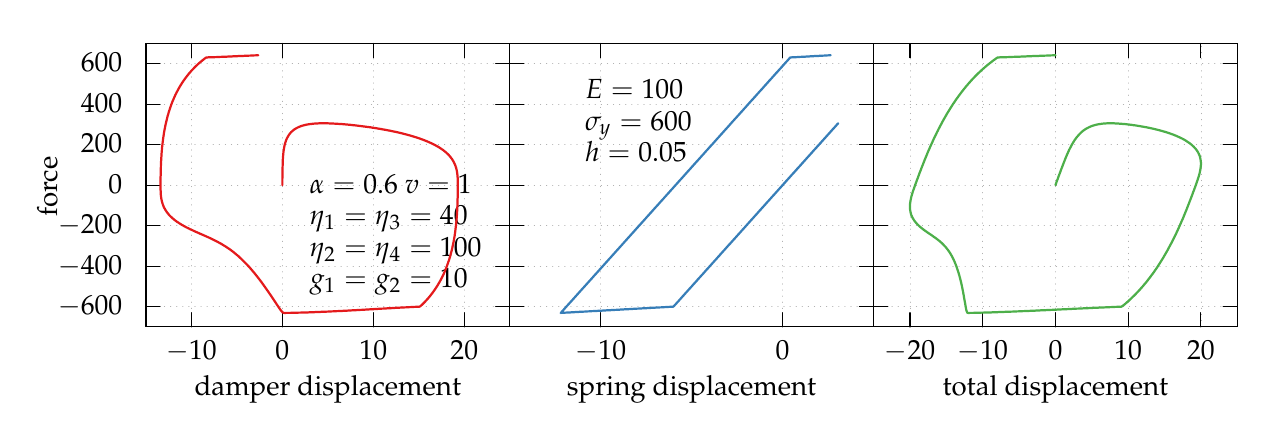
\begin{tikzpicture}[gnuplot]
%% generated with GNUPLOT 5.4p2 (Lua 5.4; terminal rev. Jun 2020, script rev. 114)
%% 11/05/21 19:40:01
\path (0.000,0.000) rectangle (14.000,4.000);
\gpcolor{color=gp lt color axes}
\gpsetlinetype{gp lt axes}
\gpsetdashtype{gp dt axes}
\gpsetlinewidth{0.50}
\draw[gp path] (0.140,0.457)--(4.759,0.457);
\gpcolor{color=gp lt color border}
\gpsetlinetype{gp lt border}
\gpsetdashtype{gp dt solid}
\gpsetlinewidth{1.00}
\draw[gp path] (0.140,0.457)--(0.320,0.457);
\draw[gp path] (4.759,0.457)--(4.579,0.457);
\node[gp node right] at (-0.044,0.457) {$-600$};
\gpcolor{color=gp lt color axes}
\gpsetlinetype{gp lt axes}
\gpsetdashtype{gp dt axes}
\gpsetlinewidth{0.50}
\draw[gp path] (0.140,0.971)--(4.759,0.971);
\gpcolor{color=gp lt color border}
\gpsetlinetype{gp lt border}
\gpsetdashtype{gp dt solid}
\gpsetlinewidth{1.00}
\draw[gp path] (0.140,0.971)--(0.320,0.971);
\draw[gp path] (4.759,0.971)--(4.579,0.971);
\node[gp node right] at (-0.044,0.971) {$-400$};
\gpcolor{color=gp lt color axes}
\gpsetlinetype{gp lt axes}
\gpsetdashtype{gp dt axes}
\gpsetlinewidth{0.50}
\draw[gp path] (0.140,1.485)--(4.759,1.485);
\gpcolor{color=gp lt color border}
\gpsetlinetype{gp lt border}
\gpsetdashtype{gp dt solid}
\gpsetlinewidth{1.00}
\draw[gp path] (0.140,1.485)--(0.320,1.485);
\draw[gp path] (4.759,1.485)--(4.579,1.485);
\node[gp node right] at (-0.044,1.485) {$-200$};
\gpcolor{color=gp lt color axes}
\gpsetlinetype{gp lt axes}
\gpsetdashtype{gp dt axes}
\gpsetlinewidth{0.50}
\draw[gp path] (0.140,2.000)--(4.759,2.000);
\gpcolor{color=gp lt color border}
\gpsetlinetype{gp lt border}
\gpsetdashtype{gp dt solid}
\gpsetlinewidth{1.00}
\draw[gp path] (0.140,2.000)--(0.320,2.000);
\draw[gp path] (4.759,2.000)--(4.579,2.000);
\node[gp node right] at (-0.044,2.000) {$0$};
\gpcolor{color=gp lt color axes}
\gpsetlinetype{gp lt axes}
\gpsetdashtype{gp dt axes}
\gpsetlinewidth{0.50}
\draw[gp path] (0.140,2.514)--(4.759,2.514);
\gpcolor{color=gp lt color border}
\gpsetlinetype{gp lt border}
\gpsetdashtype{gp dt solid}
\gpsetlinewidth{1.00}
\draw[gp path] (0.140,2.514)--(0.320,2.514);
\draw[gp path] (4.759,2.514)--(4.579,2.514);
\node[gp node right] at (-0.044,2.514) {$200$};
\gpcolor{color=gp lt color axes}
\gpsetlinetype{gp lt axes}
\gpsetdashtype{gp dt axes}
\gpsetlinewidth{0.50}
\draw[gp path] (0.140,3.028)--(4.759,3.028);
\gpcolor{color=gp lt color border}
\gpsetlinetype{gp lt border}
\gpsetdashtype{gp dt solid}
\gpsetlinewidth{1.00}
\draw[gp path] (0.140,3.028)--(0.320,3.028);
\draw[gp path] (4.759,3.028)--(4.579,3.028);
\node[gp node right] at (-0.044,3.028) {$400$};
\gpcolor{color=gp lt color axes}
\gpsetlinetype{gp lt axes}
\gpsetdashtype{gp dt axes}
\gpsetlinewidth{0.50}
\draw[gp path] (0.140,3.542)--(4.759,3.542);
\gpcolor{color=gp lt color border}
\gpsetlinetype{gp lt border}
\gpsetdashtype{gp dt solid}
\gpsetlinewidth{1.00}
\draw[gp path] (0.140,3.542)--(0.320,3.542);
\draw[gp path] (4.759,3.542)--(4.579,3.542);
\node[gp node right] at (-0.044,3.542) {$600$};
\gpcolor{color=gp lt color axes}
\gpsetlinetype{gp lt axes}
\gpsetdashtype{gp dt axes}
\gpsetlinewidth{0.50}
\draw[gp path] (0.717,0.200)--(0.717,0.380)--(0.717,3.799);
\gpcolor{color=gp lt color border}
\gpsetlinetype{gp lt border}
\gpsetdashtype{gp dt solid}
\gpsetlinewidth{1.00}
\draw[gp path] (0.717,0.200)--(0.717,0.380);
\draw[gp path] (0.717,3.799)--(0.717,3.619);
\node[gp node center] at (0.717,-0.108) {$-10$};
\gpcolor{color=gp lt color axes}
\gpsetlinetype{gp lt axes}
\gpsetdashtype{gp dt axes}
\gpsetlinewidth{0.50}
\draw[gp path] (1.872,0.200)--(1.872,3.799);
\gpcolor{color=gp lt color border}
\gpsetlinetype{gp lt border}
\gpsetdashtype{gp dt solid}
\gpsetlinewidth{1.00}
\draw[gp path] (1.872,0.200)--(1.872,0.380);
\draw[gp path] (1.872,3.799)--(1.872,3.619);
\node[gp node center] at (1.872,-0.108) {$0$};
\gpcolor{color=gp lt color axes}
\gpsetlinetype{gp lt axes}
\gpsetdashtype{gp dt axes}
\gpsetlinewidth{0.50}
\draw[gp path] (3.027,0.200)--(3.027,3.799);
\gpcolor{color=gp lt color border}
\gpsetlinetype{gp lt border}
\gpsetdashtype{gp dt solid}
\gpsetlinewidth{1.00}
\draw[gp path] (3.027,0.200)--(3.027,0.380);
\draw[gp path] (3.027,3.799)--(3.027,3.619);
\node[gp node center] at (3.027,-0.108) {$10$};
\gpcolor{color=gp lt color axes}
\gpsetlinetype{gp lt axes}
\gpsetdashtype{gp dt axes}
\gpsetlinewidth{0.50}
\draw[gp path] (4.182,0.200)--(4.182,3.799);
\gpcolor{color=gp lt color border}
\gpsetlinetype{gp lt border}
\gpsetdashtype{gp dt solid}
\gpsetlinewidth{1.00}
\draw[gp path] (4.182,0.200)--(4.182,0.380);
\draw[gp path] (4.182,3.799)--(4.182,3.619);
\node[gp node center] at (4.182,-0.108) {$20$};
\draw[gp path] (0.140,3.799)--(0.140,0.200)--(4.759,0.200)--(4.759,3.799)--cycle;
\node[gp node left] at (2.100,2.000) {$\alpha=0.6$~$v=1$};
\node[gp node left] at (2.100,1.600) {$\eta_1=\eta_3=40$};
\node[gp node left] at (2.100,1.200) {$\eta_2=\eta_4=100$};
\node[gp node left] at (2.100,0.800) {$g_1=g_2=10$};
\node[gp node left] at (5.600,3.199) {$E=100$};
\node[gp node left] at (5.600,2.799) {$\sigma_y=600$};
\node[gp node left] at (5.600,2.399) {$h=0.05$};
\node[gp node center,rotate=-270] at (-1.072,1.999) {force};
\node[gp node center] at (2.449,-0.569) {damper displacement};
\gpcolor{rgb color={0.894,0.102,0.110}}
\gpsetlinewidth{2.00}
\draw[gp path] (1.872,2.000)--(1.872,2.040)--(1.872,2.080)--(1.873,2.120)--(1.873,2.159)%
  --(1.874,2.198)--(1.875,2.236)--(1.876,2.274)--(1.877,2.311)--(1.879,2.347)--(1.882,2.381)%
  --(1.885,2.414)--(1.889,2.446)--(1.894,2.475)--(1.899,2.503)--(1.906,2.529)--(1.913,2.552)%
  --(1.921,2.574)--(1.930,2.595)--(1.940,2.613)--(1.950,2.630)--(1.961,2.646)--(1.972,2.660)%
  --(1.984,2.674)--(1.997,2.686)--(2.010,2.697)--(2.023,2.707)--(2.037,2.716)--(2.051,2.724)%
  --(2.065,2.731)--(2.079,2.738)--(2.094,2.744)--(2.109,2.750)--(2.125,2.755)--(2.140,2.759)%
  --(2.156,2.763)--(2.172,2.767)--(2.188,2.770)--(2.204,2.773)--(2.220,2.775)--(2.236,2.777)%
  --(2.253,2.779)--(2.269,2.781)--(2.286,2.782)--(2.302,2.783)--(2.319,2.784)--(2.336,2.785)%
  --(2.353,2.785)--(2.369,2.785)--(2.386,2.786)--(2.403,2.786)--(2.420,2.785)--(2.436,2.785)%
  --(2.453,2.785)--(2.470,2.784)--(2.487,2.784)--(2.504,2.783)--(2.520,2.782)--(2.537,2.781)%
  --(2.554,2.780)--(2.570,2.779)--(2.587,2.778)--(2.604,2.777)--(2.620,2.776)--(2.637,2.775)%
  --(2.653,2.773)--(2.669,2.772)--(2.686,2.770)--(2.702,2.769)--(2.718,2.767)--(2.735,2.766)%
  --(2.751,2.764)--(2.767,2.762)--(2.783,2.761)--(2.799,2.759)--(2.815,2.757)--(2.831,2.755)%
  --(2.847,2.753)--(2.862,2.751)--(2.878,2.749)--(2.894,2.747)--(2.909,2.745)--(2.925,2.743)%
  --(2.940,2.741)--(2.955,2.739)--(2.971,2.737)--(2.986,2.735)--(3.001,2.733)--(3.016,2.730)%
  --(3.031,2.728)--(3.046,2.726)--(3.061,2.723)--(3.075,2.721)--(3.090,2.718)--(3.105,2.716)%
  --(3.119,2.714)--(3.133,2.711)--(3.148,2.708)--(3.162,2.706)--(3.176,2.703)--(3.190,2.701)%
  --(3.204,2.698)--(3.218,2.695)--(3.232,2.693)--(3.246,2.690)--(3.259,2.687)--(3.273,2.684)%
  --(3.286,2.681)--(3.299,2.679)--(3.313,2.676)--(3.326,2.673)--(3.339,2.670)--(3.352,2.667)%
  --(3.365,2.664)--(3.377,2.661)--(3.390,2.658)--(3.403,2.655)--(3.415,2.651)--(3.428,2.648)%
  --(3.440,2.645)--(3.452,2.642)--(3.464,2.639)--(3.476,2.635)--(3.488,2.632)--(3.500,2.629)%
  --(3.511,2.625)--(3.523,2.622)--(3.534,2.618)--(3.546,2.615)--(3.557,2.611)--(3.568,2.608)%
  --(3.579,2.604)--(3.590,2.601)--(3.601,2.597)--(3.611,2.594)--(3.622,2.590)--(3.632,2.586)%
  --(3.643,2.582)--(3.653,2.579)--(3.663,2.575)--(3.673,2.571)--(3.683,2.567)--(3.693,2.563)%
  --(3.703,2.559)--(3.712,2.555)--(3.722,2.551)--(3.731,2.547)--(3.740,2.543)--(3.749,2.539)%
  --(3.758,2.535)--(3.767,2.531)--(3.776,2.526)--(3.785,2.522)--(3.793,2.518)--(3.802,2.514)%
  --(3.810,2.509)--(3.818,2.505)--(3.826,2.500)--(3.834,2.496)--(3.842,2.492)--(3.850,2.487)%
  --(3.857,2.482)--(3.865,2.478)--(3.872,2.473)--(3.879,2.469)--(3.886,2.464)--(3.893,2.459)%
  --(3.900,2.454)--(3.907,2.450)--(3.914,2.445)--(3.920,2.440)--(3.926,2.435)--(3.933,2.430)%
  --(3.939,2.425)--(3.945,2.420)--(3.951,2.415)--(3.957,2.410)--(3.962,2.404)--(3.968,2.399)%
  --(3.973,2.394)--(3.978,2.389)--(3.984,2.383)--(3.989,2.378)--(3.994,2.372)--(3.998,2.367)%
  --(4.003,2.361)--(4.008,2.356)--(4.012,2.350)--(4.016,2.344)--(4.021,2.339)--(4.025,2.333)%
  --(4.029,2.327)--(4.033,2.321)--(4.036,2.315)--(4.040,2.309)--(4.043,2.303)--(4.047,2.297)%
  --(4.050,2.291)--(4.053,2.285)--(4.056,2.278)--(4.059,2.272)--(4.062,2.265)--(4.065,2.259)%
  --(4.067,2.252)--(4.070,2.246)--(4.072,2.239)--(4.074,2.232)--(4.077,2.226)--(4.079,2.219)%
  --(4.081,2.212)--(4.082,2.205)--(4.084,2.197)--(4.086,2.190)--(4.087,2.183)--(4.089,2.175)%
  --(4.090,2.168)--(4.091,2.160)--(4.092,2.153)--(4.093,2.145)--(4.094,2.137)--(4.095,2.129)%
  --(4.096,2.121)--(4.097,2.112)--(4.097,2.104)--(4.098,2.095)--(4.098,2.087)--(4.098,2.078)%
  --(4.099,2.069)--(4.099,2.059)--(4.099,2.050)--(4.100,2.040)--(4.100,2.030)--(4.100,2.020)%
  --(4.100,2.010)--(4.100,1.999)--(4.100,1.989)--(4.100,1.978)--(4.100,1.966)--(4.100,1.955)%
  --(4.100,1.943)--(4.099,1.931)--(4.099,1.919)--(4.099,1.906)--(4.099,1.893)--(4.099,1.880)%
  --(4.098,1.867)--(4.098,1.854)--(4.098,1.840)--(4.097,1.826)--(4.097,1.812)--(4.097,1.797)%
  --(4.096,1.783)--(4.096,1.768)--(4.095,1.753)--(4.095,1.738)--(4.094,1.722)--(4.093,1.707)%
  --(4.092,1.691)--(4.092,1.676)--(4.091,1.660)--(4.090,1.644)--(4.089,1.627)--(4.088,1.611)%
  --(4.086,1.595)--(4.085,1.578)--(4.084,1.562)--(4.082,1.545)--(4.081,1.529)--(4.079,1.512)%
  --(4.077,1.495)--(4.075,1.478)--(4.073,1.461)--(4.071,1.444)--(4.069,1.427)--(4.067,1.410)%
  --(4.065,1.393)--(4.062,1.376)--(4.060,1.359)--(4.057,1.342)--(4.054,1.325)--(4.051,1.308)%
  --(4.048,1.291)--(4.045,1.274)--(4.041,1.257)--(4.038,1.241)--(4.034,1.224)--(4.031,1.207)%
  --(4.027,1.190)--(4.023,1.173)--(4.019,1.157)--(4.014,1.140)--(4.010,1.124)--(4.005,1.107)%
  --(4.001,1.091)--(3.996,1.074)--(3.991,1.058)--(3.986,1.042)--(3.980,1.026)--(3.975,1.010)%
  --(3.969,0.994)--(3.964,0.979)--(3.958,0.963)--(3.952,0.947)--(3.946,0.932)--(3.939,0.917)%
  --(3.933,0.901)--(3.926,0.886)--(3.920,0.871)--(3.913,0.857)--(3.906,0.842)--(3.899,0.827)%
  --(3.891,0.813)--(3.884,0.799)--(3.876,0.784)--(3.868,0.770)--(3.860,0.756)--(3.852,0.743)%
  --(3.844,0.729)--(3.836,0.715)--(3.827,0.702)--(3.818,0.689)--(3.810,0.676)--(3.801,0.663)%
  --(3.791,0.650)--(3.782,0.637)--(3.773,0.625)--(3.763,0.612)--(3.754,0.600)--(3.744,0.588)%
  --(3.734,0.576)--(3.724,0.564)--(3.713,0.552)--(3.703,0.541)--(3.692,0.529)--(3.682,0.518)%
  --(3.671,0.507)--(3.660,0.496)--(3.649,0.485)--(3.638,0.475)--(3.626,0.464)--(3.615,0.457)%
  --(3.604,0.456)--(3.592,0.456)--(3.581,0.455)--(3.569,0.455)--(3.558,0.454)--(3.546,0.454)%
  --(3.534,0.453)--(3.523,0.453)--(3.511,0.452)--(3.500,0.451)--(3.488,0.451)--(3.477,0.450)%
  --(3.465,0.450)--(3.454,0.449)--(3.442,0.448)--(3.430,0.448)--(3.419,0.447)--(3.407,0.447)%
  --(3.396,0.446)--(3.384,0.445)--(3.372,0.445)--(3.361,0.444)--(3.349,0.443)--(3.337,0.443)%
  --(3.326,0.442)--(3.314,0.442)--(3.302,0.441)--(3.291,0.440)--(3.279,0.440)--(3.267,0.439)%
  --(3.255,0.438)--(3.244,0.438)--(3.232,0.437)--(3.220,0.436)--(3.209,0.436)--(3.197,0.435)%
  --(3.185,0.434)--(3.173,0.434)--(3.161,0.433)--(3.150,0.432)--(3.138,0.432)--(3.126,0.431)%
  --(3.114,0.430)--(3.102,0.429)--(3.091,0.429)--(3.079,0.428)--(3.067,0.427)--(3.055,0.427)%
  --(3.043,0.426)--(3.031,0.425)--(3.019,0.425)--(3.007,0.424)--(2.995,0.423)--(2.984,0.423)%
  --(2.972,0.422)--(2.960,0.421)--(2.948,0.421)--(2.936,0.420)--(2.924,0.419)--(2.912,0.418)%
  --(2.900,0.418)--(2.888,0.417)--(2.876,0.416)--(2.864,0.416)--(2.852,0.415)--(2.840,0.414)%
  --(2.828,0.414)--(2.816,0.413)--(2.804,0.412)--(2.792,0.412)--(2.780,0.411)--(2.767,0.410)%
  --(2.755,0.410)--(2.743,0.409)--(2.731,0.408)--(2.719,0.408)--(2.707,0.407)--(2.695,0.406)%
  --(2.683,0.406)--(2.670,0.405)--(2.658,0.404)--(2.646,0.404)--(2.634,0.403)--(2.622,0.403)%
  --(2.609,0.402)--(2.597,0.401)--(2.585,0.401)--(2.573,0.400)--(2.561,0.400)--(2.548,0.399)%
  --(2.536,0.398)--(2.524,0.398)--(2.512,0.397)--(2.499,0.397)--(2.487,0.396)--(2.475,0.395)%
  --(2.462,0.395)--(2.450,0.394)--(2.438,0.394)--(2.425,0.393)--(2.413,0.393)--(2.401,0.392)%
  --(2.388,0.392)--(2.376,0.391)--(2.364,0.391)--(2.351,0.390)--(2.339,0.389)--(2.326,0.389)%
  --(2.314,0.389)--(2.302,0.388)--(2.289,0.388)--(2.277,0.387)--(2.264,0.387)--(2.252,0.386)%
  --(2.239,0.386)--(2.227,0.385)--(2.214,0.385)--(2.202,0.384)--(2.189,0.384)--(2.177,0.384)%
  --(2.164,0.383)--(2.152,0.383)--(2.139,0.382)--(2.127,0.382)--(2.114,0.382)--(2.101,0.381)%
  --(2.089,0.381)--(2.076,0.381)--(2.063,0.380)--(2.051,0.380)--(2.038,0.380)--(2.025,0.379)%
  --(2.013,0.379)--(2.000,0.379)--(1.987,0.379)--(1.974,0.378)--(1.961,0.378)--(1.948,0.378)%
  --(1.935,0.378)--(1.922,0.378)--(1.908,0.377)--(1.894,0.377)--(1.877,0.382)--(1.848,0.416)%
  --(1.805,0.479)--(1.761,0.546)--(1.718,0.610)--(1.677,0.669)--(1.639,0.723)--(1.604,0.772)%
  --(1.570,0.816)--(1.538,0.857)--(1.508,0.894)--(1.479,0.928)--(1.452,0.959)--(1.425,0.988)%
  --(1.400,1.014)--(1.376,1.038)--(1.353,1.061)--(1.331,1.081)--(1.310,1.101)--(1.289,1.118)%
  --(1.269,1.135)--(1.250,1.151)--(1.231,1.165)--(1.213,1.179)--(1.195,1.191)--(1.177,1.203)%
  --(1.160,1.215)--(1.144,1.225)--(1.127,1.235)--(1.111,1.245)--(1.096,1.254)--(1.080,1.263)%
  --(1.065,1.271)--(1.051,1.279)--(1.036,1.287)--(1.022,1.294)--(1.008,1.301)--(0.994,1.308)%
  --(0.981,1.314)--(0.967,1.321)--(0.954,1.327)--(0.941,1.333)--(0.929,1.339)--(0.916,1.344)%
  --(0.904,1.350)--(0.891,1.355)--(0.879,1.361)--(0.867,1.366)--(0.856,1.371)--(0.844,1.376)%
  --(0.833,1.381)--(0.821,1.386)--(0.810,1.391)--(0.799,1.396)--(0.789,1.400)--(0.778,1.405)%
  --(0.767,1.410)--(0.757,1.415)--(0.747,1.419)--(0.737,1.424)--(0.727,1.429)--(0.717,1.433)%
  --(0.707,1.438)--(0.697,1.442)--(0.688,1.447)--(0.679,1.452)--(0.669,1.456)--(0.660,1.461)%
  --(0.651,1.465)--(0.642,1.470)--(0.634,1.475)--(0.625,1.479)--(0.617,1.484)--(0.608,1.489)%
  --(0.600,1.493)--(0.592,1.498)--(0.584,1.503)--(0.576,1.507)--(0.569,1.512)--(0.561,1.517)%
  --(0.554,1.522)--(0.547,1.527)--(0.539,1.532)--(0.532,1.536)--(0.525,1.541)--(0.519,1.546)%
  --(0.512,1.551)--(0.505,1.556)--(0.499,1.561)--(0.493,1.567)--(0.486,1.572)--(0.480,1.577)%
  --(0.474,1.582)--(0.469,1.587)--(0.463,1.593)--(0.457,1.598)--(0.452,1.603)--(0.446,1.609)%
  --(0.441,1.614)--(0.436,1.619)--(0.431,1.625)--(0.426,1.631)--(0.422,1.636)--(0.417,1.642)%
  --(0.413,1.647)--(0.408,1.653)--(0.404,1.659)--(0.400,1.665)--(0.396,1.671)--(0.392,1.677)%
  --(0.388,1.683)--(0.385,1.689)--(0.381,1.695)--(0.378,1.701)--(0.374,1.707)--(0.371,1.713)%
  --(0.368,1.720)--(0.365,1.726)--(0.362,1.733)--(0.360,1.739)--(0.357,1.746)--(0.355,1.752)%
  --(0.352,1.759)--(0.350,1.766)--(0.348,1.773)--(0.346,1.780)--(0.344,1.787)--(0.342,1.794)%
  --(0.340,1.801)--(0.339,1.808)--(0.337,1.815)--(0.336,1.823)--(0.334,1.830)--(0.333,1.838)%
  --(0.332,1.846)--(0.331,1.854)--(0.330,1.862)--(0.329,1.870)--(0.328,1.878)--(0.328,1.886)%
  --(0.327,1.894)--(0.327,1.903)--(0.326,1.912)--(0.326,1.921)--(0.326,1.930)--(0.325,1.939)%
  --(0.325,1.949)--(0.325,1.958)--(0.325,1.968)--(0.325,1.978)--(0.325,1.989)--(0.324,1.999)%
  --(0.324,2.010)--(0.325,2.021)--(0.325,2.032)--(0.325,2.044)--(0.325,2.056)--(0.325,2.068)%
  --(0.325,2.080)--(0.325,2.092)--(0.325,2.105)--(0.326,2.118)--(0.326,2.131)--(0.326,2.145)%
  --(0.327,2.159)--(0.327,2.173)--(0.327,2.187)--(0.328,2.201)--(0.328,2.216)--(0.329,2.231)%
  --(0.329,2.246)--(0.330,2.261)--(0.330,2.276)--(0.331,2.292)--(0.332,2.307)--(0.333,2.323)%
  --(0.334,2.339)--(0.335,2.355)--(0.336,2.371)--(0.337,2.387)--(0.338,2.404)--(0.339,2.420)%
  --(0.341,2.437)--(0.342,2.453)--(0.344,2.470)--(0.345,2.487)--(0.347,2.503)--(0.349,2.520)%
  --(0.351,2.537)--(0.353,2.554)--(0.355,2.571)--(0.357,2.588)--(0.360,2.605)--(0.362,2.622)%
  --(0.365,2.639)--(0.367,2.656)--(0.370,2.673)--(0.373,2.690)--(0.376,2.707)--(0.380,2.724)%
  --(0.383,2.741)--(0.386,2.758)--(0.390,2.775)--(0.394,2.792)--(0.398,2.809)--(0.402,2.825)%
  --(0.406,2.842)--(0.410,2.858)--(0.414,2.875)--(0.419,2.891)--(0.424,2.908)--(0.428,2.924)%
  --(0.433,2.940)--(0.439,2.956)--(0.444,2.973)--(0.449,2.988)--(0.455,3.004)--(0.460,3.020)%
  --(0.466,3.036)--(0.472,3.051)--(0.478,3.067)--(0.485,3.082)--(0.491,3.097)--(0.498,3.112)%
  --(0.505,3.127)--(0.511,3.142)--(0.519,3.157)--(0.526,3.171)--(0.533,3.186)--(0.541,3.200)%
  --(0.548,3.214)--(0.556,3.228)--(0.564,3.242)--(0.572,3.256)--(0.580,3.270)--(0.589,3.283)%
  --(0.597,3.297)--(0.606,3.310)--(0.615,3.323)--(0.624,3.336)--(0.633,3.349)--(0.642,3.361)%
  --(0.652,3.374)--(0.661,3.386)--(0.671,3.398)--(0.681,3.411)--(0.691,3.423)--(0.701,3.434)%
  --(0.711,3.446)--(0.721,3.458)--(0.732,3.469)--(0.743,3.480)--(0.753,3.491)--(0.764,3.502)%
  --(0.775,3.513)--(0.787,3.524)--(0.798,3.534)--(0.809,3.545)--(0.821,3.555)--(0.833,3.565)%
  --(0.845,3.575)--(0.857,3.585)--(0.869,3.594)--(0.881,3.604)--(0.893,3.613)--(0.906,3.622)%
  --(0.918,3.622)--(0.931,3.623)--(0.943,3.623)--(0.956,3.624)--(0.968,3.624)--(0.981,3.624)%
  --(0.993,3.625)--(1.006,3.625)--(1.018,3.626)--(1.031,3.626)--(1.044,3.627)--(1.056,3.628)%
  --(1.069,3.628)--(1.081,3.629)--(1.094,3.629)--(1.107,3.630)--(1.119,3.630)--(1.132,3.631)%
  --(1.145,3.631)--(1.157,3.632)--(1.170,3.632)--(1.183,3.633)--(1.195,3.633)--(1.208,3.634)%
  --(1.221,3.635)--(1.233,3.635)--(1.246,3.636)--(1.259,3.636)--(1.271,3.637)--(1.284,3.637)%
  --(1.297,3.638)--(1.310,3.639)--(1.322,3.639)--(1.335,3.640)--(1.348,3.640)--(1.361,3.641)%
  --(1.374,3.641)--(1.386,3.642)--(1.399,3.643)--(1.412,3.643)--(1.425,3.644)--(1.438,3.644)%
  --(1.451,3.645)--(1.463,3.645)--(1.476,3.646)--(1.489,3.647)--(1.502,3.647)--(1.515,3.648)%
  --(1.528,3.648)--(1.541,3.649)--(1.554,3.650)--(1.567,3.650);
\gpcolor{color=gp lt color border}
\gpsetlinewidth{1.00}
\draw[gp path] (0.140,3.799)--(0.140,0.200)--(4.759,0.200)--(4.759,3.799)--cycle;
%% coordinates of the plot area
\gpdefrectangularnode{gp plot 1}{\pgfpoint{0.140cm}{0.200cm}}{\pgfpoint{4.759cm}{3.799cm}}
\gpcolor{color=gp lt color axes}
\gpsetlinetype{gp lt axes}
\gpsetdashtype{gp dt axes}
\gpsetlinewidth{0.50}
\draw[gp path] (4.760,0.457)--(9.379,0.457);
\gpcolor{color=gp lt color border}
\gpsetlinetype{gp lt border}
\gpsetdashtype{gp dt solid}
\gpsetlinewidth{1.00}
\draw[gp path] (4.760,0.457)--(4.940,0.457);
\draw[gp path] (9.379,0.457)--(9.199,0.457);
\gpcolor{color=gp lt color axes}
\gpsetlinetype{gp lt axes}
\gpsetdashtype{gp dt axes}
\gpsetlinewidth{0.50}
\draw[gp path] (4.760,0.971)--(9.379,0.971);
\gpcolor{color=gp lt color border}
\gpsetlinetype{gp lt border}
\gpsetdashtype{gp dt solid}
\gpsetlinewidth{1.00}
\draw[gp path] (4.760,0.971)--(4.940,0.971);
\draw[gp path] (9.379,0.971)--(9.199,0.971);
\gpcolor{color=gp lt color axes}
\gpsetlinetype{gp lt axes}
\gpsetdashtype{gp dt axes}
\gpsetlinewidth{0.50}
\draw[gp path] (4.760,1.485)--(9.379,1.485);
\gpcolor{color=gp lt color border}
\gpsetlinetype{gp lt border}
\gpsetdashtype{gp dt solid}
\gpsetlinewidth{1.00}
\draw[gp path] (4.760,1.485)--(4.940,1.485);
\draw[gp path] (9.379,1.485)--(9.199,1.485);
\gpcolor{color=gp lt color axes}
\gpsetlinetype{gp lt axes}
\gpsetdashtype{gp dt axes}
\gpsetlinewidth{0.50}
\draw[gp path] (4.760,2.000)--(9.379,2.000);
\gpcolor{color=gp lt color border}
\gpsetlinetype{gp lt border}
\gpsetdashtype{gp dt solid}
\gpsetlinewidth{1.00}
\draw[gp path] (4.760,2.000)--(4.940,2.000);
\draw[gp path] (9.379,2.000)--(9.199,2.000);
\gpcolor{color=gp lt color axes}
\gpsetlinetype{gp lt axes}
\gpsetdashtype{gp dt axes}
\gpsetlinewidth{0.50}
\draw[gp path] (4.760,2.514)--(9.379,2.514);
\gpcolor{color=gp lt color border}
\gpsetlinetype{gp lt border}
\gpsetdashtype{gp dt solid}
\gpsetlinewidth{1.00}
\draw[gp path] (4.760,2.514)--(4.940,2.514);
\draw[gp path] (9.379,2.514)--(9.199,2.514);
\gpcolor{color=gp lt color axes}
\gpsetlinetype{gp lt axes}
\gpsetdashtype{gp dt axes}
\gpsetlinewidth{0.50}
\draw[gp path] (4.760,3.028)--(9.379,3.028);
\gpcolor{color=gp lt color border}
\gpsetlinetype{gp lt border}
\gpsetdashtype{gp dt solid}
\gpsetlinewidth{1.00}
\draw[gp path] (4.760,3.028)--(4.940,3.028);
\draw[gp path] (9.379,3.028)--(9.199,3.028);
\gpcolor{color=gp lt color axes}
\gpsetlinetype{gp lt axes}
\gpsetdashtype{gp dt axes}
\gpsetlinewidth{0.50}
\draw[gp path] (4.760,3.542)--(9.379,3.542);
\gpcolor{color=gp lt color border}
\gpsetlinetype{gp lt border}
\gpsetdashtype{gp dt solid}
\gpsetlinewidth{1.00}
\draw[gp path] (4.760,3.542)--(4.940,3.542);
\draw[gp path] (9.379,3.542)--(9.199,3.542);
\gpcolor{color=gp lt color axes}
\gpsetlinetype{gp lt axes}
\gpsetdashtype{gp dt axes}
\gpsetlinewidth{0.50}
\draw[gp path] (5.915,0.200)--(5.915,3.799);
\gpcolor{color=gp lt color border}
\gpsetlinetype{gp lt border}
\gpsetdashtype{gp dt solid}
\gpsetlinewidth{1.00}
\draw[gp path] (5.915,0.200)--(5.915,0.380);
\draw[gp path] (5.915,3.799)--(5.915,3.619);
\node[gp node center] at (5.915,-0.108) {$-10$};
\gpcolor{color=gp lt color axes}
\gpsetlinetype{gp lt axes}
\gpsetdashtype{gp dt axes}
\gpsetlinewidth{0.50}
\draw[gp path] (8.224,0.200)--(8.224,3.799);
\gpcolor{color=gp lt color border}
\gpsetlinetype{gp lt border}
\gpsetdashtype{gp dt solid}
\gpsetlinewidth{1.00}
\draw[gp path] (8.224,0.200)--(8.224,0.380);
\draw[gp path] (8.224,3.799)--(8.224,3.619);
\node[gp node center] at (8.224,-0.108) {$0$};
\draw[gp path] (4.760,3.799)--(4.760,0.200)--(9.379,0.200)--(9.379,3.799)--cycle;
\node[gp node center] at (7.069,-0.569) {spring displacement};
\gpcolor{rgb color={0.216,0.494,0.722}}
\gpsetlinewidth{2.00}
\draw[gp path] (8.224,2.000)--(8.260,2.040)--(8.296,2.080)--(8.332,2.120)--(8.367,2.159)%
  --(8.403,2.198)--(8.437,2.236)--(8.471,2.274)--(8.504,2.311)--(8.536,2.347)--(8.567,2.381)%
  --(8.597,2.414)--(8.625,2.446)--(8.652,2.475)--(8.677,2.503)--(8.700,2.529)--(8.721,2.552)%
  --(8.741,2.574)--(8.759,2.595)--(8.776,2.613)--(8.791,2.630)--(8.805,2.646)--(8.818,2.660)%
  --(8.830,2.674)--(8.841,2.686)--(8.851,2.697)--(8.859,2.707)--(8.868,2.716)--(8.875,2.724)%
  --(8.882,2.731)--(8.888,2.738)--(8.893,2.744)--(8.898,2.750)--(8.903,2.755)--(8.907,2.759)%
  --(8.910,2.763)--(8.914,2.767)--(8.916,2.770)--(8.919,2.773)--(8.921,2.775)--(8.923,2.777)%
  --(8.925,2.779)--(8.926,2.781)--(8.927,2.782)--(8.928,2.783)--(8.929,2.784)--(8.930,2.785)%
  --(8.930,2.786)--(8.930,2.785)--(8.929,2.784)--(8.928,2.783)--(8.927,2.782)--(8.927,2.781)%
  --(8.926,2.780)--(8.925,2.779)--(8.924,2.778)--(8.923,2.777)--(8.922,2.776)--(8.921,2.775)%
  --(8.919,2.773)--(8.918,2.772)--(8.917,2.770)--(8.915,2.769)--(8.914,2.767)--(8.913,2.766)%
  --(8.911,2.764)--(8.910,2.762)--(8.908,2.761)--(8.906,2.759)--(8.905,2.757)--(8.903,2.755)%
  --(8.901,2.753)--(8.900,2.751)--(8.898,2.749)--(8.896,2.747)--(8.894,2.745)--(8.893,2.743)%
  --(8.891,2.741)--(8.889,2.739)--(8.887,2.737)--(8.885,2.735)--(8.883,2.733)--(8.881,2.730)%
  --(8.879,2.728)--(8.877,2.726)--(8.874,2.723)--(8.872,2.721)--(8.870,2.718)--(8.868,2.716)%
  --(8.866,2.714)--(8.863,2.711)--(8.861,2.708)--(8.859,2.706)--(8.857,2.703)--(8.854,2.701)%
  --(8.852,2.698)--(8.849,2.695)--(8.847,2.693)--(8.844,2.690)--(8.842,2.687)--(8.839,2.684)%
  --(8.837,2.681)--(8.834,2.679)--(8.832,2.676)--(8.829,2.673)--(8.826,2.670)--(8.824,2.667)%
  --(8.821,2.664)--(8.818,2.661)--(8.816,2.658)--(8.813,2.655)--(8.810,2.651)--(8.807,2.648)%
  --(8.804,2.645)--(8.801,2.642)--(8.798,2.639)--(8.795,2.635)--(8.792,2.632)--(8.789,2.629)%
  --(8.786,2.625)--(8.783,2.622)--(8.780,2.618)--(8.777,2.615)--(8.774,2.611)--(8.771,2.608)%
  --(8.768,2.604)--(8.764,2.601)--(8.761,2.597)--(8.758,2.594)--(8.755,2.590)--(8.751,2.586)%
  --(8.748,2.582)--(8.744,2.579)--(8.741,2.575)--(8.738,2.571)--(8.734,2.567)--(8.731,2.563)%
  --(8.727,2.559)--(8.723,2.555)--(8.720,2.551)--(8.716,2.547)--(8.713,2.543)--(8.709,2.539)%
  --(8.705,2.535)--(8.701,2.531)--(8.698,2.526)--(8.694,2.522)--(8.690,2.518)--(8.686,2.514)%
  --(8.682,2.509)--(8.678,2.505)--(8.674,2.500)--(8.670,2.496)--(8.666,2.492)--(8.662,2.487)%
  --(8.658,2.482)--(8.654,2.478)--(8.650,2.473)--(8.646,2.469)--(8.641,2.464)--(8.637,2.459)%
  --(8.633,2.454)--(8.629,2.450)--(8.624,2.445)--(8.620,2.440)--(8.615,2.435)--(8.611,2.430)%
  --(8.606,2.425)--(8.602,2.420)--(8.597,2.415)--(8.593,2.410)--(8.588,2.404)--(8.583,2.399)%
  --(8.579,2.394)--(8.574,2.389)--(8.569,2.383)--(8.564,2.378)--(8.559,2.372)--(8.554,2.367)%
  --(8.549,2.361)--(8.544,2.356)--(8.539,2.350)--(8.534,2.344)--(8.529,2.339)--(8.524,2.333)%
  --(8.518,2.327)--(8.513,2.321)--(8.508,2.315)--(8.502,2.309)--(8.497,2.303)--(8.491,2.297)%
  --(8.486,2.291)--(8.480,2.285)--(8.475,2.278)--(8.469,2.272)--(8.463,2.265)--(8.457,2.259)%
  --(8.451,2.252)--(8.446,2.246)--(8.440,2.239)--(8.433,2.232)--(8.427,2.226)--(8.421,2.219)%
  --(8.415,2.212)--(8.408,2.205)--(8.402,2.197)--(8.396,2.190)--(8.389,2.183)--(8.382,2.175)%
  --(8.376,2.168)--(8.369,2.160)--(8.362,2.153)--(8.355,2.145)--(8.348,2.137)--(8.340,2.129)%
  --(8.333,2.121)--(8.326,2.112)--(8.318,2.104)--(8.310,2.095)--(8.303,2.087)--(8.295,2.078)%
  --(8.286,2.069)--(8.278,2.059)--(8.270,2.050)--(8.261,2.040)--(8.252,2.030)--(8.243,2.020)%
  --(8.234,2.010)--(8.224,1.999)--(8.214,1.989)--(8.205,1.978)--(8.194,1.966)--(8.184,1.955)%
  --(8.173,1.943)--(8.163,1.931)--(8.152,1.919)--(8.140,1.906)--(8.129,1.893)--(8.117,1.880)%
  --(8.105,1.867)--(8.093,1.854)--(8.081,1.840)--(8.068,1.826)--(8.056,1.812)--(8.043,1.797)%
  --(8.029,1.783)--(8.016,1.768)--(8.003,1.753)--(7.989,1.738)--(7.975,1.722)--(7.961,1.707)%
  --(7.947,1.691)--(7.933,1.676)--(7.919,1.660)--(7.905,1.644)--(7.890,1.627)--(7.875,1.611)%
  --(7.861,1.595)--(7.846,1.578)--(7.831,1.562)--(7.816,1.545)--(7.801,1.529)--(7.786,1.512)%
  --(7.771,1.495)--(7.756,1.478)--(7.741,1.461)--(7.726,1.444)--(7.710,1.427)--(7.695,1.410)%
  --(7.680,1.393)--(7.664,1.376)--(7.649,1.359)--(7.634,1.342)--(7.619,1.325)--(7.603,1.308)%
  --(7.588,1.291)--(7.573,1.274)--(7.558,1.257)--(7.542,1.241)--(7.527,1.224)--(7.512,1.207)%
  --(7.497,1.190)--(7.482,1.173)--(7.467,1.157)--(7.452,1.140)--(7.437,1.124)--(7.423,1.107)%
  --(7.408,1.091)--(7.393,1.074)--(7.379,1.058)--(7.364,1.042)--(7.350,1.026)--(7.335,1.010)%
  --(7.321,0.994)--(7.307,0.979)--(7.293,0.963)--(7.279,0.947)--(7.265,0.932)--(7.251,0.917)%
  --(7.238,0.901)--(7.224,0.886)--(7.211,0.871)--(7.198,0.857)--(7.184,0.842)--(7.171,0.827)%
  --(7.158,0.813)--(7.145,0.799)--(7.133,0.784)--(7.120,0.770)--(7.107,0.756)--(7.095,0.743)%
  --(7.083,0.729)--(7.071,0.715)--(7.059,0.702)--(7.047,0.689)--(7.035,0.676)--(7.023,0.663)%
  --(7.012,0.650)--(7.000,0.637)--(6.989,0.625)--(6.978,0.612)--(6.967,0.600)--(6.956,0.588)%
  --(6.945,0.576)--(6.935,0.564)--(6.924,0.552)--(6.914,0.541)--(6.904,0.529)--(6.893,0.518)%
  --(6.883,0.507)--(6.874,0.496)--(6.864,0.485)--(6.854,0.475)--(6.845,0.464)--(6.835,0.457)%
  --(6.826,0.456)--(6.817,0.456)--(6.807,0.455)--(6.797,0.455)--(6.787,0.454)--(6.777,0.454)%
  --(6.767,0.453)--(6.757,0.453)--(6.747,0.452)--(6.736,0.451)--(6.726,0.451)--(6.715,0.450)%
  --(6.705,0.450)--(6.694,0.449)--(6.683,0.448)--(6.672,0.448)--(6.661,0.447)--(6.650,0.447)%
  --(6.639,0.446)--(6.628,0.445)--(6.617,0.445)--(6.605,0.444)--(6.594,0.443)--(6.582,0.443)%
  --(6.571,0.442)--(6.559,0.442)--(6.548,0.441)--(6.536,0.440)--(6.524,0.440)--(6.512,0.439)%
  --(6.500,0.438)--(6.489,0.438)--(6.477,0.437)--(6.465,0.436)--(6.453,0.436)--(6.440,0.435)%
  --(6.428,0.434)--(6.416,0.434)--(6.404,0.433)--(6.392,0.432)--(6.380,0.432)--(6.367,0.431)%
  --(6.355,0.430)--(6.343,0.429)--(6.330,0.429)--(6.318,0.428)--(6.306,0.427)--(6.293,0.427)%
  --(6.281,0.426)--(6.268,0.425)--(6.256,0.425)--(6.244,0.424)--(6.231,0.423)--(6.219,0.423)%
  --(6.207,0.422)--(6.194,0.421)--(6.182,0.421)--(6.169,0.420)--(6.157,0.419)--(6.145,0.418)%
  --(6.132,0.418)--(6.120,0.417)--(6.108,0.416)--(6.096,0.416)--(6.083,0.415)--(6.071,0.414)%
  --(6.059,0.414)--(6.047,0.413)--(6.035,0.412)--(6.023,0.412)--(6.011,0.411)--(5.999,0.410)%
  --(5.987,0.410)--(5.975,0.409)--(5.963,0.408)--(5.952,0.408)--(5.940,0.407)--(5.928,0.406)%
  --(5.917,0.406)--(5.905,0.405)--(5.894,0.404)--(5.882,0.404)--(5.871,0.403)--(5.860,0.403)%
  --(5.848,0.402)--(5.837,0.401)--(5.826,0.401)--(5.815,0.400)--(5.804,0.400)--(5.794,0.399)%
  --(5.783,0.398)--(5.772,0.398)--(5.762,0.397)--(5.751,0.397)--(5.741,0.396)--(5.730,0.395)%
  --(5.720,0.395)--(5.710,0.394)--(5.700,0.394)--(5.690,0.393)--(5.681,0.393)--(5.671,0.392)%
  --(5.661,0.392)--(5.652,0.391)--(5.643,0.391)--(5.633,0.390)--(5.624,0.389)--(5.615,0.389)%
  --(5.606,0.389)--(5.598,0.388)--(5.589,0.388)--(5.581,0.387)--(5.572,0.387)--(5.564,0.386)%
  --(5.556,0.386)--(5.548,0.385)--(5.540,0.385)--(5.533,0.384)--(5.525,0.384)--(5.518,0.384)%
  --(5.511,0.383)--(5.504,0.383)--(5.497,0.382)--(5.490,0.382)--(5.484,0.382)--(5.477,0.381)%
  --(5.471,0.381)--(5.465,0.381)--(5.459,0.380)--(5.453,0.380)--(5.448,0.380)--(5.443,0.379)%
  --(5.438,0.379)--(5.433,0.379)--(5.428,0.379)--(5.424,0.378)--(5.420,0.378)--(5.416,0.378)%
  --(5.413,0.378)--(5.410,0.378)--(5.408,0.377)--(5.407,0.377)--(5.412,0.382)--(5.442,0.416)%
  --(5.498,0.479)--(5.559,0.546)--(5.616,0.610)--(5.669,0.669)--(5.718,0.723)--(5.762,0.772)%
  --(5.802,0.816)--(5.838,0.857)--(5.872,0.894)--(5.902,0.928)--(5.930,0.959)--(5.956,0.988)%
  --(5.979,1.014)--(6.001,1.038)--(6.021,1.061)--(6.040,1.081)--(6.057,1.101)--(6.073,1.118)%
  --(6.088,1.135)--(6.102,1.151)--(6.115,1.165)--(6.127,1.179)--(6.139,1.191)--(6.149,1.203)%
  --(6.160,1.215)--(6.169,1.225)--(6.178,1.235)--(6.187,1.245)--(6.195,1.254)--(6.203,1.263)%
  --(6.210,1.271)--(6.217,1.279)--(6.224,1.287)--(6.231,1.294)--(6.237,1.301)--(6.243,1.308)%
  --(6.249,1.314)--(6.255,1.321)--(6.260,1.327)--(6.266,1.333)--(6.271,1.339)--(6.276,1.344)%
  --(6.281,1.350)--(6.286,1.355)--(6.291,1.361)--(6.295,1.366)--(6.300,1.371)--(6.304,1.376)%
  --(6.309,1.381)--(6.313,1.386)--(6.318,1.391)--(6.322,1.396)--(6.326,1.400)--(6.331,1.405)%
  --(6.335,1.410)--(6.339,1.415)--(6.343,1.419)--(6.347,1.424)--(6.352,1.429)--(6.356,1.433)%
  --(6.360,1.438)--(6.364,1.442)--(6.368,1.447)--(6.372,1.452)--(6.376,1.456)--(6.381,1.461)%
  --(6.385,1.465)--(6.389,1.470)--(6.393,1.475)--(6.397,1.479)--(6.401,1.484)--(6.406,1.489)%
  --(6.410,1.493)--(6.414,1.498)--(6.418,1.503)--(6.423,1.507)--(6.427,1.512)--(6.431,1.517)%
  --(6.436,1.522)--(6.440,1.527)--(6.444,1.532)--(6.449,1.536)--(6.453,1.541)--(6.458,1.546)%
  --(6.462,1.551)--(6.467,1.556)--(6.471,1.561)--(6.476,1.567)--(6.480,1.572)--(6.485,1.577)%
  --(6.490,1.582)--(6.494,1.587)--(6.499,1.593)--(6.504,1.598)--(6.509,1.603)--(6.513,1.609)%
  --(6.518,1.614)--(6.523,1.619)--(6.528,1.625)--(6.533,1.631)--(6.538,1.636)--(6.543,1.642)%
  --(6.548,1.647)--(6.554,1.653)--(6.559,1.659)--(6.564,1.665)--(6.569,1.671)--(6.575,1.677)%
  --(6.580,1.683)--(6.585,1.689)--(6.591,1.695)--(6.596,1.701)--(6.602,1.707)--(6.608,1.713)%
  --(6.613,1.720)--(6.619,1.726)--(6.625,1.733)--(6.631,1.739)--(6.637,1.746)--(6.643,1.752)%
  --(6.649,1.759)--(6.655,1.766)--(6.661,1.773)--(6.667,1.780)--(6.673,1.787)--(6.680,1.794)%
  --(6.686,1.801)--(6.693,1.808)--(6.699,1.815)--(6.706,1.823)--(6.713,1.830)--(6.720,1.838)%
  --(6.726,1.846)--(6.734,1.854)--(6.741,1.862)--(6.748,1.870)--(6.755,1.878)--(6.763,1.886)%
  --(6.770,1.894)--(6.778,1.903)--(6.786,1.912)--(6.794,1.921)--(6.802,1.930)--(6.810,1.939)%
  --(6.819,1.949)--(6.828,1.958)--(6.836,1.968)--(6.846,1.978)--(6.855,1.989)--(6.864,1.999)%
  --(6.874,2.010)--(6.884,2.021)--(6.894,2.032)--(6.904,2.044)--(6.915,2.056)--(6.926,2.068)%
  --(6.937,2.080)--(6.948,2.092)--(6.960,2.105)--(6.971,2.118)--(6.983,2.131)--(6.995,2.145)%
  --(7.008,2.159)--(7.020,2.173)--(7.033,2.187)--(7.046,2.201)--(7.059,2.216)--(7.072,2.231)%
  --(7.086,2.246)--(7.099,2.261)--(7.113,2.276)--(7.127,2.292)--(7.141,2.307)--(7.155,2.323)%
  --(7.170,2.339)--(7.184,2.355)--(7.198,2.371)--(7.213,2.387)--(7.228,2.404)--(7.242,2.420)%
  --(7.257,2.437)--(7.272,2.453)--(7.287,2.470)--(7.302,2.487)--(7.317,2.503)--(7.333,2.520)%
  --(7.348,2.537)--(7.363,2.554)--(7.378,2.571)--(7.393,2.588)--(7.409,2.605)--(7.424,2.622)%
  --(7.439,2.639)--(7.455,2.656)--(7.470,2.673)--(7.485,2.690)--(7.500,2.707)--(7.516,2.724)%
  --(7.531,2.741)--(7.546,2.758)--(7.561,2.775)--(7.576,2.792)--(7.591,2.809)--(7.606,2.825)%
  --(7.621,2.842)--(7.636,2.858)--(7.651,2.875)--(7.666,2.891)--(7.681,2.908)--(7.695,2.924)%
  --(7.710,2.940)--(7.724,2.956)--(7.739,2.973)--(7.753,2.988)--(7.767,3.004)--(7.781,3.020)%
  --(7.795,3.036)--(7.809,3.051)--(7.823,3.067)--(7.837,3.082)--(7.851,3.097)--(7.864,3.112)%
  --(7.878,3.127)--(7.891,3.142)--(7.904,3.157)--(7.917,3.171)--(7.930,3.186)--(7.943,3.200)%
  --(7.956,3.214)--(7.969,3.228)--(7.981,3.242)--(7.993,3.256)--(8.006,3.270)--(8.018,3.283)%
  --(8.030,3.297)--(8.042,3.310)--(8.053,3.323)--(8.065,3.336)--(8.077,3.349)--(8.088,3.361)%
  --(8.099,3.374)--(8.110,3.386)--(8.121,3.398)--(8.132,3.411)--(8.143,3.423)--(8.154,3.434)%
  --(8.164,3.446)--(8.175,3.458)--(8.185,3.469)--(8.195,3.480)--(8.205,3.491)--(8.215,3.502)%
  --(8.224,3.513)--(8.234,3.524)--(8.243,3.534)--(8.253,3.545)--(8.262,3.555)--(8.271,3.565)%
  --(8.280,3.575)--(8.289,3.585)--(8.297,3.594)--(8.306,3.604)--(8.314,3.613)--(8.323,3.622)%
  --(8.331,3.622)--(8.340,3.623)--(8.348,3.623)--(8.357,3.624)--(8.365,3.624)--(8.374,3.624)%
  --(8.383,3.625)--(8.392,3.625)--(8.401,3.626)--(8.410,3.626)--(8.419,3.627)--(8.429,3.628)%
  --(8.438,3.628)--(8.448,3.629)--(8.457,3.629)--(8.467,3.630)--(8.476,3.630)--(8.486,3.631)%
  --(8.496,3.631)--(8.505,3.632)--(8.515,3.632)--(8.525,3.633)--(8.535,3.633)--(8.545,3.634)%
  --(8.555,3.635)--(8.565,3.635)--(8.575,3.636)--(8.586,3.636)--(8.596,3.637)--(8.606,3.637)%
  --(8.616,3.638)--(8.627,3.639)--(8.637,3.639)--(8.647,3.640)--(8.658,3.640)--(8.668,3.641)%
  --(8.678,3.641)--(8.689,3.642)--(8.699,3.643)--(8.710,3.643)--(8.720,3.644)--(8.731,3.644)%
  --(8.741,3.645)--(8.752,3.645)--(8.762,3.646)--(8.772,3.647)--(8.783,3.647)--(8.793,3.648)%
  --(8.804,3.648)--(8.814,3.649)--(8.824,3.650)--(8.835,3.650);
\gpcolor{color=gp lt color border}
\gpsetlinewidth{1.00}
\draw[gp path] (4.760,3.799)--(4.760,0.200)--(9.379,0.200)--(9.379,3.799)--cycle;
%% coordinates of the plot area
\gpdefrectangularnode{gp plot 2}{\pgfpoint{4.760cm}{0.200cm}}{\pgfpoint{9.379cm}{3.799cm}}
\gpcolor{color=gp lt color axes}
\gpsetlinetype{gp lt axes}
\gpsetdashtype{gp dt axes}
\gpsetlinewidth{0.50}
\draw[gp path] (9.380,0.457)--(13.999,0.457);
\gpcolor{color=gp lt color border}
\gpsetlinetype{gp lt border}
\gpsetdashtype{gp dt solid}
\gpsetlinewidth{1.00}
\draw[gp path] (9.380,0.457)--(9.560,0.457);
\draw[gp path] (13.999,0.457)--(13.819,0.457);
\gpcolor{color=gp lt color axes}
\gpsetlinetype{gp lt axes}
\gpsetdashtype{gp dt axes}
\gpsetlinewidth{0.50}
\draw[gp path] (9.380,0.971)--(13.999,0.971);
\gpcolor{color=gp lt color border}
\gpsetlinetype{gp lt border}
\gpsetdashtype{gp dt solid}
\gpsetlinewidth{1.00}
\draw[gp path] (9.380,0.971)--(9.560,0.971);
\draw[gp path] (13.999,0.971)--(13.819,0.971);
\gpcolor{color=gp lt color axes}
\gpsetlinetype{gp lt axes}
\gpsetdashtype{gp dt axes}
\gpsetlinewidth{0.50}
\draw[gp path] (9.380,1.485)--(13.999,1.485);
\gpcolor{color=gp lt color border}
\gpsetlinetype{gp lt border}
\gpsetdashtype{gp dt solid}
\gpsetlinewidth{1.00}
\draw[gp path] (9.380,1.485)--(9.560,1.485);
\draw[gp path] (13.999,1.485)--(13.819,1.485);
\gpcolor{color=gp lt color axes}
\gpsetlinetype{gp lt axes}
\gpsetdashtype{gp dt axes}
\gpsetlinewidth{0.50}
\draw[gp path] (9.380,2.000)--(13.999,2.000);
\gpcolor{color=gp lt color border}
\gpsetlinetype{gp lt border}
\gpsetdashtype{gp dt solid}
\gpsetlinewidth{1.00}
\draw[gp path] (9.380,2.000)--(9.560,2.000);
\draw[gp path] (13.999,2.000)--(13.819,2.000);
\gpcolor{color=gp lt color axes}
\gpsetlinetype{gp lt axes}
\gpsetdashtype{gp dt axes}
\gpsetlinewidth{0.50}
\draw[gp path] (9.380,2.514)--(13.999,2.514);
\gpcolor{color=gp lt color border}
\gpsetlinetype{gp lt border}
\gpsetdashtype{gp dt solid}
\gpsetlinewidth{1.00}
\draw[gp path] (9.380,2.514)--(9.560,2.514);
\draw[gp path] (13.999,2.514)--(13.819,2.514);
\gpcolor{color=gp lt color axes}
\gpsetlinetype{gp lt axes}
\gpsetdashtype{gp dt axes}
\gpsetlinewidth{0.50}
\draw[gp path] (9.380,3.028)--(13.999,3.028);
\gpcolor{color=gp lt color border}
\gpsetlinetype{gp lt border}
\gpsetdashtype{gp dt solid}
\gpsetlinewidth{1.00}
\draw[gp path] (9.380,3.028)--(9.560,3.028);
\draw[gp path] (13.999,3.028)--(13.819,3.028);
\gpcolor{color=gp lt color axes}
\gpsetlinetype{gp lt axes}
\gpsetdashtype{gp dt axes}
\gpsetlinewidth{0.50}
\draw[gp path] (9.380,3.542)--(13.999,3.542);
\gpcolor{color=gp lt color border}
\gpsetlinetype{gp lt border}
\gpsetdashtype{gp dt solid}
\gpsetlinewidth{1.00}
\draw[gp path] (9.380,3.542)--(9.560,3.542);
\draw[gp path] (13.999,3.542)--(13.819,3.542);
\gpcolor{color=gp lt color axes}
\gpsetlinetype{gp lt axes}
\gpsetdashtype{gp dt axes}
\gpsetlinewidth{0.50}
\draw[gp path] (9.842,0.200)--(9.842,3.799);
\gpcolor{color=gp lt color border}
\gpsetlinetype{gp lt border}
\gpsetdashtype{gp dt solid}
\gpsetlinewidth{1.00}
\draw[gp path] (9.842,0.200)--(9.842,0.380);
\draw[gp path] (9.842,3.799)--(9.842,3.619);
\node[gp node center] at (9.842,-0.108) {$-20$};
\gpcolor{color=gp lt color axes}
\gpsetlinetype{gp lt axes}
\gpsetdashtype{gp dt axes}
\gpsetlinewidth{0.50}
\draw[gp path] (10.766,0.200)--(10.766,3.799);
\gpcolor{color=gp lt color border}
\gpsetlinetype{gp lt border}
\gpsetdashtype{gp dt solid}
\gpsetlinewidth{1.00}
\draw[gp path] (10.766,0.200)--(10.766,0.380);
\draw[gp path] (10.766,3.799)--(10.766,3.619);
\node[gp node center] at (10.766,-0.108) {$-10$};
\gpcolor{color=gp lt color axes}
\gpsetlinetype{gp lt axes}
\gpsetdashtype{gp dt axes}
\gpsetlinewidth{0.50}
\draw[gp path] (11.690,0.200)--(11.690,3.799);
\gpcolor{color=gp lt color border}
\gpsetlinetype{gp lt border}
\gpsetdashtype{gp dt solid}
\gpsetlinewidth{1.00}
\draw[gp path] (11.690,0.200)--(11.690,0.380);
\draw[gp path] (11.690,3.799)--(11.690,3.619);
\node[gp node center] at (11.690,-0.108) {$0$};
\gpcolor{color=gp lt color axes}
\gpsetlinetype{gp lt axes}
\gpsetdashtype{gp dt axes}
\gpsetlinewidth{0.50}
\draw[gp path] (12.613,0.200)--(12.613,3.799);
\gpcolor{color=gp lt color border}
\gpsetlinetype{gp lt border}
\gpsetdashtype{gp dt solid}
\gpsetlinewidth{1.00}
\draw[gp path] (12.613,0.200)--(12.613,0.380);
\draw[gp path] (12.613,3.799)--(12.613,3.619);
\node[gp node center] at (12.613,-0.108) {$10$};
\gpcolor{color=gp lt color axes}
\gpsetlinetype{gp lt axes}
\gpsetdashtype{gp dt axes}
\gpsetlinewidth{0.50}
\draw[gp path] (13.537,0.200)--(13.537,0.380)--(13.537,3.799);
\gpcolor{color=gp lt color border}
\gpsetlinetype{gp lt border}
\gpsetdashtype{gp dt solid}
\gpsetlinewidth{1.00}
\draw[gp path] (13.537,0.200)--(13.537,0.380);
\draw[gp path] (13.537,3.799)--(13.537,3.619);
\node[gp node center] at (13.537,-0.108) {$20$};
\draw[gp path] (9.380,3.799)--(9.380,0.200)--(13.999,0.200)--(13.999,3.799)--cycle;
\node[gp node center] at (11.689,-0.569) {total displacement};
\gpcolor{rgb color={0.302,0.686,0.290}}
\gpsetlinewidth{2.00}
\draw[gp path] (11.690,2.000)--(11.704,2.040)--(11.719,2.080)--(11.733,2.120)--(11.748,2.159)%
  --(11.762,2.198)--(11.777,2.236)--(11.791,2.274)--(11.806,2.311)--(11.820,2.347)--(11.834,2.381)%
  --(11.849,2.414)--(11.863,2.446)--(11.878,2.475)--(11.892,2.503)--(11.907,2.529)--(11.921,2.552)%
  --(11.935,2.574)--(11.950,2.595)--(11.964,2.613)--(11.979,2.630)--(11.993,2.646)--(12.007,2.660)%
  --(12.021,2.674)--(12.036,2.686)--(12.050,2.697)--(12.064,2.707)--(12.078,2.716)--(12.093,2.724)%
  --(12.107,2.731)--(12.121,2.738)--(12.135,2.744)--(12.149,2.750)--(12.163,2.755)--(12.177,2.759)%
  --(12.191,2.763)--(12.205,2.767)--(12.219,2.770)--(12.233,2.773)--(12.247,2.775)--(12.260,2.777)%
  --(12.274,2.779)--(12.288,2.781)--(12.302,2.782)--(12.315,2.783)--(12.329,2.784)--(12.343,2.785)%
  --(12.356,2.785)--(12.370,2.785)--(12.383,2.786)--(12.397,2.786)--(12.410,2.785)--(12.423,2.785)%
  --(12.437,2.785)--(12.450,2.784)--(12.463,2.784)--(12.476,2.783)--(12.489,2.782)--(12.502,2.781)%
  --(12.515,2.780)--(12.528,2.779)--(12.541,2.778)--(12.554,2.777)--(12.567,2.776)--(12.580,2.775)%
  --(12.592,2.773)--(12.605,2.772)--(12.617,2.770)--(12.630,2.769)--(12.642,2.767)--(12.655,2.766)%
  --(12.667,2.764)--(12.679,2.762)--(12.692,2.761)--(12.704,2.759)--(12.716,2.757)--(12.728,2.755)%
  --(12.740,2.753)--(12.752,2.751)--(12.764,2.749)--(12.775,2.747)--(12.787,2.745)--(12.799,2.743)%
  --(12.810,2.741)--(12.822,2.739)--(12.833,2.737)--(12.845,2.735)--(12.856,2.733)--(12.867,2.730)%
  --(12.878,2.728)--(12.889,2.726)--(12.900,2.723)--(12.911,2.721)--(12.922,2.718)--(12.933,2.716)%
  --(12.944,2.714)--(12.954,2.711)--(12.965,2.708)--(12.975,2.706)--(12.986,2.703)--(12.996,2.701)%
  --(13.006,2.698)--(13.016,2.695)--(13.026,2.693)--(13.036,2.690)--(13.046,2.687)--(13.056,2.684)%
  --(13.066,2.681)--(13.075,2.679)--(13.085,2.676)--(13.094,2.673)--(13.104,2.670)--(13.113,2.667)%
  --(13.122,2.664)--(13.131,2.661)--(13.140,2.658)--(13.149,2.655)--(13.158,2.651)--(13.167,2.648)%
  --(13.176,2.645)--(13.184,2.642)--(13.193,2.639)--(13.201,2.635)--(13.209,2.632)--(13.218,2.629)%
  --(13.226,2.625)--(13.234,2.622)--(13.242,2.618)--(13.249,2.615)--(13.257,2.611)--(13.265,2.608)%
  --(13.272,2.604)--(13.280,2.601)--(13.287,2.597)--(13.294,2.594)--(13.302,2.590)--(13.309,2.586)%
  --(13.316,2.582)--(13.322,2.579)--(13.329,2.575)--(13.336,2.571)--(13.342,2.567)--(13.349,2.563)%
  --(13.355,2.559)--(13.361,2.555)--(13.367,2.551)--(13.373,2.547)--(13.379,2.543)--(13.385,2.539)%
  --(13.391,2.535)--(13.396,2.531)--(13.402,2.526)--(13.407,2.522)--(13.413,2.518)--(13.418,2.514)%
  --(13.423,2.509)--(13.428,2.505)--(13.433,2.500)--(13.437,2.496)--(13.442,2.492)--(13.447,2.487)%
  --(13.451,2.482)--(13.455,2.478)--(13.460,2.473)--(13.464,2.469)--(13.468,2.464)--(13.472,2.459)%
  --(13.475,2.454)--(13.479,2.450)--(13.483,2.445)--(13.486,2.440)--(13.489,2.435)--(13.493,2.430)%
  --(13.496,2.425)--(13.499,2.420)--(13.502,2.415)--(13.504,2.410)--(13.507,2.404)--(13.510,2.399)%
  --(13.512,2.394)--(13.514,2.389)--(13.517,2.383)--(13.519,2.378)--(13.521,2.372)--(13.523,2.367)%
  --(13.524,2.361)--(13.526,2.356)--(13.527,2.350)--(13.529,2.344)--(13.530,2.339)--(13.531,2.333)%
  --(13.532,2.327)--(13.533,2.321)--(13.534,2.315)--(13.535,2.309)--(13.536,2.303)--(13.536,2.297)%
  --(13.537,2.291)--(13.537,2.285)--(13.537,2.278)--(13.537,2.272)--(13.537,2.265)--(13.537,2.259)%
  --(13.537,2.252)--(13.536,2.246)--(13.536,2.239)--(13.535,2.232)--(13.534,2.226)--(13.533,2.219)%
  --(13.532,2.212)--(13.531,2.205)--(13.530,2.197)--(13.529,2.190)--(13.527,2.183)--(13.526,2.175)%
  --(13.524,2.168)--(13.523,2.160)--(13.521,2.153)--(13.519,2.145)--(13.517,2.137)--(13.514,2.129)%
  --(13.512,2.121)--(13.510,2.112)--(13.507,2.104)--(13.504,2.095)--(13.502,2.087)--(13.499,2.078)%
  --(13.496,2.069)--(13.493,2.059)--(13.489,2.050)--(13.486,2.040)--(13.483,2.030)--(13.479,2.020)%
  --(13.475,2.010)--(13.472,1.999)--(13.468,1.989)--(13.464,1.978)--(13.460,1.966)--(13.455,1.955)%
  --(13.451,1.943)--(13.447,1.931)--(13.442,1.919)--(13.437,1.906)--(13.433,1.893)--(13.428,1.880)%
  --(13.423,1.867)--(13.418,1.854)--(13.413,1.840)--(13.407,1.826)--(13.402,1.812)--(13.396,1.797)%
  --(13.391,1.783)--(13.385,1.768)--(13.379,1.753)--(13.373,1.738)--(13.367,1.722)--(13.361,1.707)%
  --(13.355,1.691)--(13.349,1.676)--(13.342,1.660)--(13.336,1.644)--(13.329,1.627)--(13.322,1.611)%
  --(13.316,1.595)--(13.309,1.578)--(13.302,1.562)--(13.294,1.545)--(13.287,1.529)--(13.280,1.512)%
  --(13.272,1.495)--(13.265,1.478)--(13.257,1.461)--(13.249,1.444)--(13.242,1.427)--(13.234,1.410)%
  --(13.226,1.393)--(13.218,1.376)--(13.209,1.359)--(13.201,1.342)--(13.193,1.325)--(13.184,1.308)%
  --(13.176,1.291)--(13.167,1.274)--(13.158,1.257)--(13.149,1.241)--(13.140,1.224)--(13.131,1.207)%
  --(13.122,1.190)--(13.113,1.173)--(13.104,1.157)--(13.094,1.140)--(13.085,1.124)--(13.075,1.107)%
  --(13.066,1.091)--(13.056,1.074)--(13.046,1.058)--(13.036,1.042)--(13.026,1.026)--(13.016,1.010)%
  --(13.006,0.994)--(12.996,0.979)--(12.986,0.963)--(12.975,0.947)--(12.965,0.932)--(12.954,0.917)%
  --(12.944,0.901)--(12.933,0.886)--(12.922,0.871)--(12.911,0.857)--(12.900,0.842)--(12.889,0.827)%
  --(12.878,0.813)--(12.867,0.799)--(12.856,0.784)--(12.845,0.770)--(12.833,0.756)--(12.822,0.743)%
  --(12.810,0.729)--(12.799,0.715)--(12.787,0.702)--(12.775,0.689)--(12.764,0.676)--(12.752,0.663)%
  --(12.740,0.650)--(12.728,0.637)--(12.716,0.625)--(12.704,0.612)--(12.692,0.600)--(12.679,0.588)%
  --(12.667,0.576)--(12.655,0.564)--(12.642,0.552)--(12.630,0.541)--(12.617,0.529)--(12.605,0.518)%
  --(12.592,0.507)--(12.580,0.496)--(12.567,0.485)--(12.554,0.475)--(12.541,0.464)--(12.528,0.457)%
  --(12.515,0.456)--(12.502,0.456)--(12.489,0.455)--(12.476,0.455)--(12.463,0.454)--(12.450,0.454)%
  --(12.437,0.453)--(12.423,0.453)--(12.410,0.452)--(12.397,0.451)--(12.383,0.451)--(12.370,0.450)%
  --(12.356,0.450)--(12.343,0.449)--(12.329,0.448)--(12.315,0.448)--(12.302,0.447)--(12.288,0.447)%
  --(12.274,0.446)--(12.260,0.445)--(12.247,0.445)--(12.233,0.444)--(12.219,0.443)--(12.205,0.443)%
  --(12.191,0.442)--(12.177,0.442)--(12.163,0.441)--(12.149,0.440)--(12.135,0.440)--(12.121,0.439)%
  --(12.107,0.438)--(12.093,0.438)--(12.078,0.437)--(12.064,0.436)--(12.050,0.436)--(12.036,0.435)%
  --(12.021,0.434)--(12.007,0.434)--(11.993,0.433)--(11.979,0.432)--(11.964,0.432)--(11.950,0.431)%
  --(11.935,0.430)--(11.921,0.429)--(11.907,0.429)--(11.892,0.428)--(11.878,0.427)--(11.863,0.427)%
  --(11.849,0.426)--(11.834,0.425)--(11.820,0.425)--(11.806,0.424)--(11.791,0.423)--(11.777,0.423)%
  --(11.762,0.422)--(11.748,0.421)--(11.733,0.421)--(11.719,0.420)--(11.704,0.419)--(11.690,0.418)%
  --(11.675,0.418)--(11.660,0.417)--(11.646,0.416)--(11.631,0.416)--(11.617,0.415)--(11.602,0.414)%
  --(11.588,0.414)--(11.573,0.413)--(11.559,0.412)--(11.545,0.412)--(11.530,0.411)--(11.516,0.410)%
  --(11.501,0.410)--(11.487,0.409)--(11.472,0.408)--(11.458,0.408)--(11.444,0.407)--(11.429,0.406)%
  --(11.415,0.406)--(11.400,0.405)--(11.386,0.404)--(11.372,0.404)--(11.358,0.403)--(11.343,0.403)%
  --(11.329,0.402)--(11.315,0.401)--(11.301,0.401)--(11.286,0.400)--(11.272,0.400)--(11.258,0.399)%
  --(11.244,0.398)--(11.230,0.398)--(11.216,0.397)--(11.202,0.397)--(11.188,0.396)--(11.174,0.395)%
  --(11.160,0.395)--(11.146,0.394)--(11.132,0.394)--(11.119,0.393)--(11.105,0.393)--(11.091,0.392)%
  --(11.077,0.392)--(11.064,0.391)--(11.050,0.391)--(11.036,0.390)--(11.023,0.389)--(11.009,0.389)%
  --(10.996,0.389)--(10.982,0.388)--(10.969,0.388)--(10.956,0.387)--(10.942,0.387)--(10.929,0.386)%
  --(10.916,0.386)--(10.903,0.385)--(10.890,0.385)--(10.877,0.384)--(10.864,0.384)--(10.851,0.384)%
  --(10.838,0.383)--(10.825,0.383)--(10.812,0.382)--(10.799,0.382)--(10.787,0.382)--(10.774,0.381)%
  --(10.762,0.381)--(10.749,0.381)--(10.737,0.380)--(10.724,0.380)--(10.712,0.380)--(10.700,0.379)%
  --(10.687,0.379)--(10.675,0.379)--(10.663,0.379)--(10.651,0.378)--(10.639,0.378)--(10.627,0.378)%
  --(10.615,0.378)--(10.604,0.378)--(10.592,0.377)--(10.580,0.377)--(10.569,0.382)--(10.557,0.416)%
  --(10.546,0.479)--(10.534,0.546)--(10.523,0.610)--(10.512,0.669)--(10.501,0.723)--(10.490,0.772)%
  --(10.479,0.816)--(10.468,0.857)--(10.457,0.894)--(10.446,0.928)--(10.435,0.959)--(10.425,0.988)%
  --(10.414,1.014)--(10.404,1.038)--(10.393,1.061)--(10.383,1.081)--(10.373,1.101)--(10.363,1.118)%
  --(10.353,1.135)--(10.343,1.151)--(10.333,1.165)--(10.323,1.179)--(10.313,1.191)--(10.304,1.203)%
  --(10.294,1.215)--(10.285,1.225)--(10.275,1.235)--(10.266,1.245)--(10.257,1.254)--(10.248,1.263)%
  --(10.239,1.271)--(10.230,1.279)--(10.221,1.287)--(10.212,1.294)--(10.203,1.301)--(10.195,1.308)%
  --(10.186,1.314)--(10.178,1.321)--(10.170,1.327)--(10.161,1.333)--(10.153,1.339)--(10.145,1.344)%
  --(10.137,1.350)--(10.130,1.355)--(10.122,1.361)--(10.114,1.366)--(10.107,1.371)--(10.099,1.376)%
  --(10.092,1.381)--(10.085,1.386)--(10.077,1.391)--(10.070,1.396)--(10.063,1.400)--(10.057,1.405)%
  --(10.050,1.410)--(10.043,1.415)--(10.037,1.419)--(10.030,1.424)--(10.024,1.429)--(10.018,1.433)%
  --(10.012,1.438)--(10.006,1.442)--(10.000,1.447)--(9.994,1.452)--(9.988,1.456)--(9.983,1.461)%
  --(9.977,1.465)--(9.972,1.470)--(9.966,1.475)--(9.961,1.479)--(9.956,1.484)--(9.951,1.489)%
  --(9.946,1.493)--(9.942,1.498)--(9.937,1.503)--(9.932,1.507)--(9.928,1.512)--(9.924,1.517)%
  --(9.919,1.522)--(9.915,1.527)--(9.911,1.532)--(9.907,1.536)--(9.904,1.541)--(9.900,1.546)%
  --(9.896,1.551)--(9.893,1.556)--(9.890,1.561)--(9.886,1.567)--(9.883,1.572)--(9.880,1.577)%
  --(9.877,1.582)--(9.875,1.587)--(9.872,1.593)--(9.869,1.598)--(9.867,1.603)--(9.865,1.609)%
  --(9.862,1.614)--(9.860,1.619)--(9.858,1.625)--(9.856,1.631)--(9.855,1.636)--(9.853,1.642)%
  --(9.852,1.647)--(9.850,1.653)--(9.849,1.659)--(9.848,1.665)--(9.847,1.671)--(9.846,1.677)%
  --(9.845,1.683)--(9.844,1.689)--(9.843,1.695)--(9.843,1.701)--(9.842,1.707)--(9.842,1.713)%
  --(9.842,1.720)--(9.842,1.726)--(9.842,1.733)--(9.842,1.739)--(9.842,1.746)--(9.843,1.752)%
  --(9.843,1.759)--(9.844,1.766)--(9.845,1.773)--(9.846,1.780)--(9.847,1.787)--(9.848,1.794)%
  --(9.849,1.801)--(9.850,1.808)--(9.852,1.815)--(9.853,1.823)--(9.855,1.830)--(9.856,1.838)%
  --(9.858,1.846)--(9.860,1.854)--(9.862,1.862)--(9.865,1.870)--(9.867,1.878)--(9.869,1.886)%
  --(9.872,1.894)--(9.875,1.903)--(9.877,1.912)--(9.880,1.921)--(9.883,1.930)--(9.886,1.939)%
  --(9.890,1.949)--(9.893,1.958)--(9.896,1.968)--(9.900,1.978)--(9.904,1.989)--(9.907,1.999)%
  --(9.911,2.010)--(9.915,2.021)--(9.919,2.032)--(9.924,2.044)--(9.928,2.056)--(9.932,2.068)%
  --(9.937,2.080)--(9.942,2.092)--(9.946,2.105)--(9.951,2.118)--(9.956,2.131)--(9.961,2.145)%
  --(9.966,2.159)--(9.972,2.173)--(9.977,2.187)--(9.983,2.201)--(9.988,2.216)--(9.994,2.231)%
  --(10.000,2.246)--(10.006,2.261)--(10.012,2.276)--(10.018,2.292)--(10.024,2.307)--(10.030,2.323)%
  --(10.037,2.339)--(10.043,2.355)--(10.050,2.371)--(10.057,2.387)--(10.063,2.404)--(10.070,2.420)%
  --(10.077,2.437)--(10.085,2.453)--(10.092,2.470)--(10.099,2.487)--(10.107,2.503)--(10.114,2.520)%
  --(10.122,2.537)--(10.130,2.554)--(10.137,2.571)--(10.145,2.588)--(10.153,2.605)--(10.161,2.622)%
  --(10.170,2.639)--(10.178,2.656)--(10.186,2.673)--(10.195,2.690)--(10.203,2.707)--(10.212,2.724)%
  --(10.221,2.741)--(10.230,2.758)--(10.239,2.775)--(10.248,2.792)--(10.257,2.809)--(10.266,2.825)%
  --(10.275,2.842)--(10.285,2.858)--(10.294,2.875)--(10.304,2.891)--(10.313,2.908)--(10.323,2.924)%
  --(10.333,2.940)--(10.343,2.956)--(10.353,2.973)--(10.363,2.988)--(10.373,3.004)--(10.383,3.020)%
  --(10.393,3.036)--(10.404,3.051)--(10.414,3.067)--(10.425,3.082)--(10.435,3.097)--(10.446,3.112)%
  --(10.457,3.127)--(10.468,3.142)--(10.479,3.157)--(10.490,3.171)--(10.501,3.186)--(10.512,3.200)%
  --(10.523,3.214)--(10.534,3.228)--(10.546,3.242)--(10.557,3.256)--(10.569,3.270)--(10.580,3.283)%
  --(10.592,3.297)--(10.604,3.310)--(10.615,3.323)--(10.627,3.336)--(10.639,3.349)--(10.651,3.361)%
  --(10.663,3.374)--(10.675,3.386)--(10.687,3.398)--(10.700,3.411)--(10.712,3.423)--(10.724,3.434)%
  --(10.737,3.446)--(10.749,3.458)--(10.762,3.469)--(10.774,3.480)--(10.787,3.491)--(10.799,3.502)%
  --(10.812,3.513)--(10.825,3.524)--(10.838,3.534)--(10.851,3.545)--(10.864,3.555)--(10.877,3.565)%
  --(10.890,3.575)--(10.903,3.585)--(10.916,3.594)--(10.929,3.604)--(10.942,3.613)--(10.956,3.622)%
  --(10.969,3.622)--(10.982,3.623)--(10.996,3.623)--(11.009,3.624)--(11.023,3.624)--(11.036,3.624)%
  --(11.050,3.625)--(11.064,3.625)--(11.077,3.626)--(11.091,3.626)--(11.105,3.627)--(11.119,3.628)%
  --(11.132,3.628)--(11.146,3.629)--(11.160,3.629)--(11.174,3.630)--(11.188,3.630)--(11.202,3.631)%
  --(11.216,3.631)--(11.230,3.632)--(11.244,3.632)--(11.258,3.633)--(11.272,3.633)--(11.286,3.634)%
  --(11.301,3.635)--(11.315,3.635)--(11.329,3.636)--(11.343,3.636)--(11.358,3.637)--(11.372,3.637)%
  --(11.386,3.638)--(11.400,3.639)--(11.415,3.639)--(11.429,3.640)--(11.444,3.640)--(11.458,3.641)%
  --(11.472,3.641)--(11.487,3.642)--(11.501,3.643)--(11.516,3.643)--(11.530,3.644)--(11.545,3.644)%
  --(11.559,3.645)--(11.573,3.645)--(11.588,3.646)--(11.602,3.647)--(11.617,3.647)--(11.631,3.648)%
  --(11.646,3.648)--(11.660,3.649)--(11.675,3.650)--(11.690,3.650);
\gpcolor{color=gp lt color border}
\gpsetlinewidth{1.00}
\draw[gp path] (9.380,3.799)--(9.380,0.200)--(13.999,0.200)--(13.999,3.799)--cycle;
%% coordinates of the plot area
\gpdefrectangularnode{gp plot 3}{\pgfpoint{9.380cm}{0.200cm}}{\pgfpoint{13.999cm}{3.799cm}}
\end{tikzpicture}
%% gnuplot variables

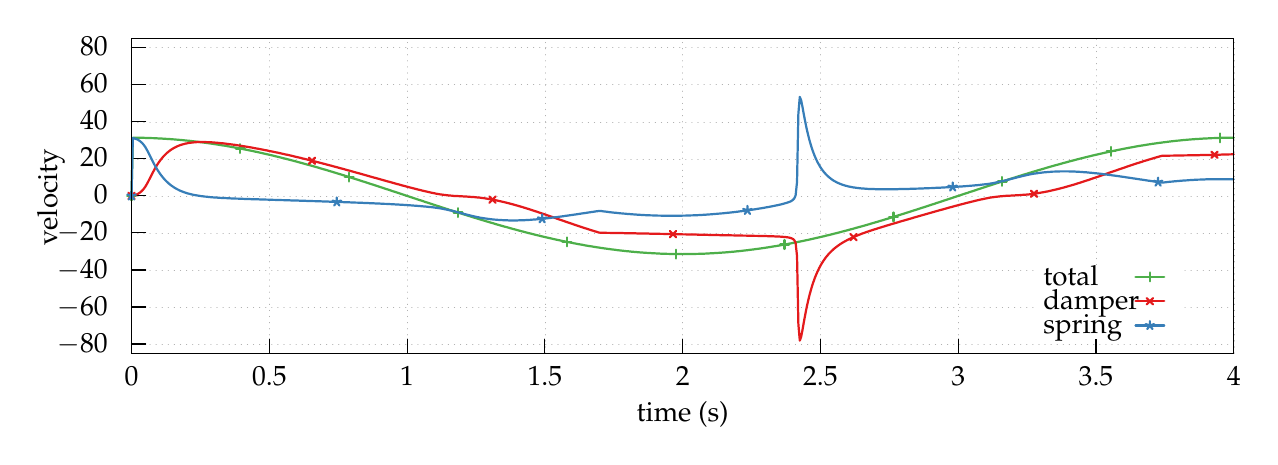
\begin{tikzpicture}[gnuplot]
%% generated with GNUPLOT 5.4p2 (Lua 5.4; terminal rev. Jun 2020, script rev. 114)
%% 11/09/21 03:15:51
\path (0.000,0.000) rectangle (14.000,4.000);
\gpcolor{color=gp lt color axes}
\gpsetlinetype{gp lt axes}
\gpsetdashtype{gp dt axes}
\gpsetlinewidth{0.50}
\draw[gp path] (0.000,0.118)--(13.999,0.118);
\gpcolor{color=gp lt color border}
\gpsetlinetype{gp lt border}
\gpsetdashtype{gp dt solid}
\gpsetlinewidth{1.00}
\draw[gp path] (0.000,0.118)--(0.180,0.118);
\node[gp node right] at (-0.184,0.118) {$-80$};
\gpcolor{color=gp lt color axes}
\gpsetlinetype{gp lt axes}
\gpsetdashtype{gp dt axes}
\gpsetlinewidth{0.50}
\draw[gp path] (0.000,0.588)--(11.463,0.588);
\draw[gp path] (13.299,0.588)--(13.999,0.588);
\gpcolor{color=gp lt color border}
\gpsetlinetype{gp lt border}
\gpsetdashtype{gp dt solid}
\gpsetlinewidth{1.00}
\draw[gp path] (0.000,0.588)--(0.180,0.588);
\node[gp node right] at (-0.184,0.588) {$-60$};
\gpcolor{color=gp lt color axes}
\gpsetlinetype{gp lt axes}
\gpsetdashtype{gp dt axes}
\gpsetlinewidth{0.50}
\draw[gp path] (0.000,1.059)--(11.463,1.059);
\draw[gp path] (13.299,1.059)--(13.999,1.059);
\gpcolor{color=gp lt color border}
\gpsetlinetype{gp lt border}
\gpsetdashtype{gp dt solid}
\gpsetlinewidth{1.00}
\draw[gp path] (0.000,1.059)--(0.180,1.059);
\node[gp node right] at (-0.184,1.059) {$-40$};
\gpcolor{color=gp lt color axes}
\gpsetlinetype{gp lt axes}
\gpsetdashtype{gp dt axes}
\gpsetlinewidth{0.50}
\draw[gp path] (0.000,1.529)--(13.999,1.529);
\gpcolor{color=gp lt color border}
\gpsetlinetype{gp lt border}
\gpsetdashtype{gp dt solid}
\gpsetlinewidth{1.00}
\draw[gp path] (0.000,1.529)--(0.180,1.529);
\node[gp node right] at (-0.184,1.529) {$-20$};
\gpcolor{color=gp lt color axes}
\gpsetlinetype{gp lt axes}
\gpsetdashtype{gp dt axes}
\gpsetlinewidth{0.50}
\draw[gp path] (0.000,2.000)--(13.999,2.000);
\gpcolor{color=gp lt color border}
\gpsetlinetype{gp lt border}
\gpsetdashtype{gp dt solid}
\gpsetlinewidth{1.00}
\draw[gp path] (0.000,2.000)--(0.180,2.000);
\node[gp node right] at (-0.184,2.000) {$0$};
\gpcolor{color=gp lt color axes}
\gpsetlinetype{gp lt axes}
\gpsetdashtype{gp dt axes}
\gpsetlinewidth{0.50}
\draw[gp path] (0.000,2.470)--(13.999,2.470);
\gpcolor{color=gp lt color border}
\gpsetlinetype{gp lt border}
\gpsetdashtype{gp dt solid}
\gpsetlinewidth{1.00}
\draw[gp path] (0.000,2.470)--(0.180,2.470);
\node[gp node right] at (-0.184,2.470) {$20$};
\gpcolor{color=gp lt color axes}
\gpsetlinetype{gp lt axes}
\gpsetdashtype{gp dt axes}
\gpsetlinewidth{0.50}
\draw[gp path] (0.000,2.940)--(13.999,2.940);
\gpcolor{color=gp lt color border}
\gpsetlinetype{gp lt border}
\gpsetdashtype{gp dt solid}
\gpsetlinewidth{1.00}
\draw[gp path] (0.000,2.940)--(0.180,2.940);
\node[gp node right] at (-0.184,2.940) {$40$};
\gpcolor{color=gp lt color axes}
\gpsetlinetype{gp lt axes}
\gpsetdashtype{gp dt axes}
\gpsetlinewidth{0.50}
\draw[gp path] (0.000,3.411)--(13.999,3.411);
\gpcolor{color=gp lt color border}
\gpsetlinetype{gp lt border}
\gpsetdashtype{gp dt solid}
\gpsetlinewidth{1.00}
\draw[gp path] (0.000,3.411)--(0.180,3.411);
\node[gp node right] at (-0.184,3.411) {$60$};
\gpcolor{color=gp lt color axes}
\gpsetlinetype{gp lt axes}
\gpsetdashtype{gp dt axes}
\gpsetlinewidth{0.50}
\draw[gp path] (0.000,3.881)--(13.999,3.881);
\gpcolor{color=gp lt color border}
\gpsetlinetype{gp lt border}
\gpsetdashtype{gp dt solid}
\gpsetlinewidth{1.00}
\draw[gp path] (0.000,3.881)--(0.180,3.881);
\node[gp node right] at (-0.184,3.881) {$80$};
\gpcolor{color=gp lt color axes}
\gpsetlinetype{gp lt axes}
\gpsetdashtype{gp dt axes}
\gpsetlinewidth{0.50}
\draw[gp path] (0.000,0.000)--(0.000,3.999);
\gpcolor{color=gp lt color border}
\gpsetlinetype{gp lt border}
\gpsetdashtype{gp dt solid}
\gpsetlinewidth{1.00}
\draw[gp path] (0.000,0.000)--(0.000,0.180);
\node[gp node center] at (0.000,-0.308) {$0$};
\gpcolor{color=gp lt color axes}
\gpsetlinetype{gp lt axes}
\gpsetdashtype{gp dt axes}
\gpsetlinewidth{0.50}
\draw[gp path] (1.750,0.000)--(1.750,3.999);
\gpcolor{color=gp lt color border}
\gpsetlinetype{gp lt border}
\gpsetdashtype{gp dt solid}
\gpsetlinewidth{1.00}
\draw[gp path] (1.750,0.000)--(1.750,0.180);
\node[gp node center] at (1.750,-0.308) {$0.5$};
\gpcolor{color=gp lt color axes}
\gpsetlinetype{gp lt axes}
\gpsetdashtype{gp dt axes}
\gpsetlinewidth{0.50}
\draw[gp path] (3.500,0.000)--(3.500,3.999);
\gpcolor{color=gp lt color border}
\gpsetlinetype{gp lt border}
\gpsetdashtype{gp dt solid}
\gpsetlinewidth{1.00}
\draw[gp path] (3.500,0.000)--(3.500,0.180);
\node[gp node center] at (3.500,-0.308) {$1$};
\gpcolor{color=gp lt color axes}
\gpsetlinetype{gp lt axes}
\gpsetdashtype{gp dt axes}
\gpsetlinewidth{0.50}
\draw[gp path] (5.250,0.000)--(5.250,3.999);
\gpcolor{color=gp lt color border}
\gpsetlinetype{gp lt border}
\gpsetdashtype{gp dt solid}
\gpsetlinewidth{1.00}
\draw[gp path] (5.250,0.000)--(5.250,0.180);
\node[gp node center] at (5.250,-0.308) {$1.5$};
\gpcolor{color=gp lt color axes}
\gpsetlinetype{gp lt axes}
\gpsetdashtype{gp dt axes}
\gpsetlinewidth{0.50}
\draw[gp path] (7.000,0.000)--(7.000,3.999);
\gpcolor{color=gp lt color border}
\gpsetlinetype{gp lt border}
\gpsetdashtype{gp dt solid}
\gpsetlinewidth{1.00}
\draw[gp path] (7.000,0.000)--(7.000,0.180);
\node[gp node center] at (7.000,-0.308) {$2$};
\gpcolor{color=gp lt color axes}
\gpsetlinetype{gp lt axes}
\gpsetdashtype{gp dt axes}
\gpsetlinewidth{0.50}
\draw[gp path] (8.749,0.000)--(8.749,3.999);
\gpcolor{color=gp lt color border}
\gpsetlinetype{gp lt border}
\gpsetdashtype{gp dt solid}
\gpsetlinewidth{1.00}
\draw[gp path] (8.749,0.000)--(8.749,0.180);
\node[gp node center] at (8.749,-0.308) {$2.5$};
\gpcolor{color=gp lt color axes}
\gpsetlinetype{gp lt axes}
\gpsetdashtype{gp dt axes}
\gpsetlinewidth{0.50}
\draw[gp path] (10.499,0.000)--(10.499,3.999);
\gpcolor{color=gp lt color border}
\gpsetlinetype{gp lt border}
\gpsetdashtype{gp dt solid}
\gpsetlinewidth{1.00}
\draw[gp path] (10.499,0.000)--(10.499,0.180);
\node[gp node center] at (10.499,-0.308) {$3$};
\gpcolor{color=gp lt color axes}
\gpsetlinetype{gp lt axes}
\gpsetdashtype{gp dt axes}
\gpsetlinewidth{0.50}
\draw[gp path] (12.249,0.000)--(12.249,0.200);
\draw[gp path] (12.249,1.124)--(12.249,3.999);
\gpcolor{color=gp lt color border}
\gpsetlinetype{gp lt border}
\gpsetdashtype{gp dt solid}
\gpsetlinewidth{1.00}
\draw[gp path] (12.249,0.000)--(12.249,0.180);
\node[gp node center] at (12.249,-0.308) {$3.5$};
\gpcolor{color=gp lt color axes}
\gpsetlinetype{gp lt axes}
\gpsetdashtype{gp dt axes}
\gpsetlinewidth{0.50}
\draw[gp path] (13.999,0.000)--(13.999,3.999);
\gpcolor{color=gp lt color border}
\gpsetlinetype{gp lt border}
\gpsetdashtype{gp dt solid}
\gpsetlinewidth{1.00}
\draw[gp path] (13.999,0.000)--(13.999,0.180);
\node[gp node center] at (13.999,-0.308) {$4$};
\draw[gp path] (0.000,3.999)--(0.000,0.000)--(13.999,0.000)--(13.999,3.999)--cycle;
\node[gp node center,rotate=-270] at (-1.028,1.999) {velocity};
\node[gp node center] at (6.999,-0.769) {time (\si{\second})};
\gpcolor{rgb color={0.302,0.686,0.290}}
\gpsetlinewidth{2.00}
\draw[gp path] (0.000,2.000)--(0.017,2.738)--(0.035,2.738)--(0.052,2.738)--(0.070,2.738)%
  --(0.087,2.738)--(0.105,2.738)--(0.122,2.737)--(0.140,2.737)--(0.157,2.737)--(0.175,2.736)%
  --(0.192,2.736)--(0.210,2.735)--(0.227,2.735)--(0.245,2.734)--(0.262,2.733)--(0.280,2.733)%
  --(0.297,2.732)--(0.315,2.731)--(0.332,2.730)--(0.350,2.729)--(0.367,2.728)--(0.385,2.728)%
  --(0.402,2.726)--(0.420,2.725)--(0.437,2.724)--(0.455,2.723)--(0.472,2.722)--(0.490,2.721)%
  --(0.507,2.719)--(0.525,2.718)--(0.542,2.717)--(0.560,2.715)--(0.577,2.714)--(0.595,2.712)%
  --(0.612,2.711)--(0.630,2.709)--(0.647,2.708)--(0.665,2.706)--(0.682,2.704)--(0.700,2.702)%
  --(0.717,2.701)--(0.735,2.699)--(0.752,2.697)--(0.770,2.695)--(0.787,2.693)--(0.805,2.691)%
  --(0.822,2.689)--(0.840,2.687)--(0.857,2.684)--(0.875,2.682)--(0.892,2.680)--(0.910,2.678)%
  --(0.927,2.675)--(0.945,2.673)--(0.962,2.671)--(0.980,2.668)--(0.997,2.666)--(1.015,2.663)%
  --(1.032,2.661)--(1.050,2.658)--(1.067,2.655)--(1.085,2.653)--(1.102,2.650)--(1.120,2.647)%
  --(1.137,2.644)--(1.155,2.641)--(1.172,2.639)--(1.190,2.636)--(1.207,2.633)--(1.225,2.630)%
  --(1.242,2.627)--(1.260,2.623)--(1.277,2.620)--(1.295,2.617)--(1.312,2.614)--(1.330,2.611)%
  --(1.347,2.607)--(1.365,2.604)--(1.382,2.601)--(1.400,2.597)--(1.417,2.594)--(1.435,2.590)%
  --(1.452,2.587)--(1.470,2.583)--(1.487,2.580)--(1.505,2.576)--(1.522,2.573)--(1.540,2.569)%
  --(1.557,2.565)--(1.575,2.561)--(1.592,2.558)--(1.610,2.554)--(1.627,2.550)--(1.645,2.546)%
  --(1.662,2.542)--(1.680,2.538)--(1.697,2.534)--(1.715,2.530)--(1.732,2.526)--(1.750,2.522)%
  --(1.767,2.518)--(1.785,2.514)--(1.802,2.510)--(1.820,2.505)--(1.837,2.501)--(1.855,2.497)%
  --(1.872,2.493)--(1.890,2.488)--(1.907,2.484)--(1.925,2.479)--(1.942,2.475)--(1.960,2.471)%
  --(1.977,2.466)--(1.995,2.462)--(2.012,2.457)--(2.030,2.452)--(2.047,2.448)--(2.065,2.443)%
  --(2.082,2.439)--(2.100,2.434)--(2.117,2.429)--(2.135,2.424)--(2.152,2.420)--(2.170,2.415)%
  --(2.187,2.410)--(2.205,2.405)--(2.222,2.400)--(2.240,2.395)--(2.257,2.391)--(2.275,2.386)%
  --(2.292,2.381)--(2.310,2.376)--(2.327,2.371)--(2.345,2.366)--(2.362,2.361)--(2.380,2.356)%
  --(2.397,2.350)--(2.415,2.345)--(2.432,2.340)--(2.450,2.335)--(2.467,2.330)--(2.485,2.325)%
  --(2.502,2.319)--(2.520,2.314)--(2.537,2.309)--(2.555,2.304)--(2.572,2.298)--(2.590,2.293)%
  --(2.607,2.288)--(2.625,2.282)--(2.642,2.277)--(2.660,2.272)--(2.677,2.266)--(2.695,2.261)%
  --(2.712,2.255)--(2.730,2.250)--(2.747,2.244)--(2.765,2.239)--(2.782,2.233)--(2.800,2.228)%
  --(2.817,2.222)--(2.835,2.217)--(2.852,2.211)--(2.870,2.206)--(2.887,2.200)--(2.905,2.195)%
  --(2.922,2.189)--(2.940,2.183)--(2.957,2.178)--(2.975,2.172)--(2.992,2.166)--(3.010,2.161)%
  --(3.027,2.155)--(3.045,2.149)--(3.062,2.144)--(3.080,2.138)--(3.097,2.132)--(3.115,2.127)%
  --(3.132,2.121)--(3.150,2.115)--(3.167,2.109)--(3.185,2.104)--(3.202,2.098)--(3.220,2.092)%
  --(3.237,2.086)--(3.255,2.081)--(3.272,2.075)--(3.290,2.069)--(3.307,2.063)--(3.325,2.057)%
  --(3.342,2.052)--(3.360,2.046)--(3.377,2.040)--(3.395,2.034)--(3.412,2.029)--(3.430,2.023)%
  --(3.447,2.017)--(3.465,2.011)--(3.482,2.005)--(3.500,1.999)--(3.517,1.994)--(3.535,1.988)%
  --(3.552,1.982)--(3.570,1.976)--(3.587,1.970)--(3.605,1.965)--(3.622,1.959)--(3.640,1.953)%
  --(3.657,1.947)--(3.675,1.942)--(3.692,1.936)--(3.710,1.930)--(3.727,1.924)--(3.745,1.918)%
  --(3.762,1.913)--(3.780,1.907)--(3.797,1.901)--(3.815,1.895)--(3.832,1.890)--(3.850,1.884)%
  --(3.867,1.878)--(3.885,1.872)--(3.902,1.867)--(3.920,1.861)--(3.937,1.855)--(3.955,1.850)%
  --(3.972,1.844)--(3.990,1.838)--(4.007,1.833)--(4.025,1.827)--(4.042,1.821)--(4.060,1.816)%
  --(4.077,1.810)--(4.095,1.804)--(4.112,1.799)--(4.130,1.793)--(4.147,1.788)--(4.165,1.782)%
  --(4.182,1.777)--(4.200,1.771)--(4.217,1.766)--(4.235,1.760)--(4.252,1.755)--(4.270,1.749)%
  --(4.287,1.744)--(4.305,1.738)--(4.322,1.733)--(4.340,1.727)--(4.357,1.722)--(4.375,1.717)%
  --(4.392,1.711)--(4.410,1.706)--(4.427,1.701)--(4.445,1.695)--(4.462,1.690)--(4.480,1.685)%
  --(4.497,1.680)--(4.515,1.674)--(4.532,1.669)--(4.550,1.664)--(4.567,1.659)--(4.585,1.654)%
  --(4.602,1.649)--(4.620,1.643)--(4.637,1.638)--(4.655,1.633)--(4.672,1.628)--(4.690,1.623)%
  --(4.707,1.618)--(4.725,1.613)--(4.742,1.608)--(4.760,1.604)--(4.777,1.599)--(4.795,1.594)%
  --(4.812,1.589)--(4.830,1.584)--(4.847,1.579)--(4.865,1.575)--(4.882,1.570)--(4.900,1.565)%
  --(4.917,1.560)--(4.935,1.556)--(4.952,1.551)--(4.970,1.547)--(4.987,1.542)--(5.005,1.537)%
  --(5.022,1.533)--(5.040,1.528)--(5.057,1.524)--(5.075,1.520)--(5.092,1.515)--(5.110,1.511)%
  --(5.127,1.506)--(5.145,1.502)--(5.162,1.498)--(5.180,1.494)--(5.197,1.489)--(5.215,1.485)%
  --(5.232,1.481)--(5.250,1.477)--(5.267,1.473)--(5.285,1.469)--(5.302,1.465)--(5.320,1.461)%
  --(5.337,1.457)--(5.355,1.453)--(5.372,1.449)--(5.390,1.445)--(5.407,1.441)--(5.425,1.438)%
  --(5.442,1.434)--(5.460,1.430)--(5.477,1.426)--(5.495,1.423)--(5.512,1.419)--(5.530,1.416)%
  --(5.547,1.412)--(5.565,1.409)--(5.582,1.405)--(5.600,1.402)--(5.617,1.398)--(5.635,1.395)%
  --(5.652,1.392)--(5.670,1.388)--(5.687,1.385)--(5.705,1.382)--(5.722,1.379)--(5.740,1.376)%
  --(5.757,1.372)--(5.775,1.369)--(5.792,1.366)--(5.810,1.363)--(5.827,1.360)--(5.845,1.358)%
  --(5.862,1.355)--(5.880,1.352)--(5.897,1.349)--(5.915,1.346)--(5.932,1.344)--(5.950,1.341)%
  --(5.967,1.338)--(5.985,1.336)--(6.002,1.333)--(6.020,1.331)--(6.037,1.328)--(6.055,1.326)%
  --(6.072,1.324)--(6.090,1.321)--(6.107,1.319)--(6.125,1.317)--(6.142,1.315)--(6.160,1.312)%
  --(6.177,1.310)--(6.195,1.308)--(6.212,1.306)--(6.230,1.304)--(6.247,1.302)--(6.265,1.300)%
  --(6.282,1.298)--(6.300,1.297)--(6.317,1.295)--(6.335,1.293)--(6.352,1.291)--(6.370,1.290)%
  --(6.387,1.288)--(6.405,1.287)--(6.422,1.285)--(6.440,1.284)--(6.457,1.282)--(6.475,1.281)%
  --(6.492,1.280)--(6.510,1.278)--(6.527,1.277)--(6.545,1.276)--(6.562,1.275)--(6.580,1.274)%
  --(6.597,1.273)--(6.615,1.271)--(6.632,1.271)--(6.650,1.270)--(6.667,1.269)--(6.685,1.268)%
  --(6.702,1.267)--(6.720,1.266)--(6.737,1.266)--(6.755,1.265)--(6.772,1.264)--(6.790,1.264)%
  --(6.807,1.263)--(6.825,1.263)--(6.842,1.262)--(6.860,1.262)--(6.877,1.262)--(6.895,1.261)%
  --(6.912,1.261)--(6.930,1.261)--(6.947,1.261)--(6.965,1.261)--(6.982,1.261)--(7.000,1.260)%
  --(7.017,1.261)--(7.034,1.261)--(7.052,1.261)--(7.069,1.261)--(7.087,1.261)--(7.104,1.261)%
  --(7.122,1.262)--(7.139,1.262)--(7.157,1.262)--(7.174,1.263)--(7.192,1.263)--(7.209,1.264)%
  --(7.227,1.264)--(7.244,1.265)--(7.262,1.266)--(7.279,1.266)--(7.297,1.267)--(7.314,1.268)%
  --(7.332,1.269)--(7.349,1.270)--(7.367,1.271)--(7.384,1.271)--(7.402,1.273)--(7.419,1.274)%
  --(7.437,1.275)--(7.454,1.276)--(7.472,1.277)--(7.489,1.278)--(7.507,1.280)--(7.524,1.281)%
  --(7.542,1.282)--(7.559,1.284)--(7.577,1.285)--(7.594,1.287)--(7.612,1.288)--(7.629,1.290)%
  --(7.647,1.291)--(7.664,1.293)--(7.682,1.295)--(7.699,1.297)--(7.717,1.298)--(7.734,1.300)%
  --(7.752,1.302)--(7.769,1.304)--(7.787,1.306)--(7.804,1.308)--(7.822,1.310)--(7.839,1.312)%
  --(7.857,1.315)--(7.874,1.317)--(7.892,1.319)--(7.909,1.321)--(7.927,1.324)--(7.944,1.326)%
  --(7.962,1.328)--(7.979,1.331)--(7.997,1.333)--(8.014,1.336)--(8.032,1.338)--(8.049,1.341)%
  --(8.067,1.344)--(8.084,1.346)--(8.102,1.349)--(8.119,1.352)--(8.137,1.355)--(8.154,1.358)%
  --(8.172,1.360)--(8.189,1.363)--(8.207,1.366)--(8.224,1.369)--(8.242,1.372)--(8.259,1.376)%
  --(8.277,1.379)--(8.294,1.382)--(8.312,1.385)--(8.329,1.388)--(8.347,1.392)--(8.364,1.395)%
  --(8.382,1.398)--(8.399,1.402)--(8.417,1.405)--(8.434,1.409)--(8.452,1.412)--(8.469,1.416)%
  --(8.487,1.419)--(8.504,1.423)--(8.522,1.426)--(8.539,1.430)--(8.557,1.434)--(8.574,1.438)%
  --(8.592,1.441)--(8.609,1.445)--(8.627,1.449)--(8.644,1.453)--(8.662,1.457)--(8.679,1.461)%
  --(8.697,1.465)--(8.714,1.469)--(8.732,1.473)--(8.749,1.477)--(8.767,1.481)--(8.784,1.485)%
  --(8.802,1.489)--(8.819,1.494)--(8.837,1.498)--(8.854,1.502)--(8.872,1.506)--(8.889,1.511)%
  --(8.907,1.515)--(8.924,1.520)--(8.942,1.524)--(8.959,1.528)--(8.977,1.533)--(8.994,1.537)%
  --(9.012,1.542)--(9.029,1.547)--(9.047,1.551)--(9.064,1.556)--(9.082,1.560)--(9.099,1.565)%
  --(9.117,1.570)--(9.134,1.575)--(9.152,1.579)--(9.169,1.584)--(9.187,1.589)--(9.204,1.594)%
  --(9.222,1.599)--(9.239,1.604)--(9.257,1.608)--(9.274,1.613)--(9.292,1.618)--(9.309,1.623)%
  --(9.327,1.628)--(9.344,1.633)--(9.362,1.638)--(9.379,1.643)--(9.397,1.649)--(9.414,1.654)%
  --(9.432,1.659)--(9.449,1.664)--(9.467,1.669)--(9.484,1.674)--(9.502,1.680)--(9.519,1.685)%
  --(9.537,1.690)--(9.554,1.695)--(9.572,1.701)--(9.589,1.706)--(9.607,1.711)--(9.624,1.717)%
  --(9.642,1.722)--(9.659,1.727)--(9.677,1.733)--(9.694,1.738)--(9.712,1.744)--(9.729,1.749)%
  --(9.747,1.755)--(9.764,1.760)--(9.782,1.766)--(9.799,1.771)--(9.817,1.777)--(9.834,1.782)%
  --(9.852,1.788)--(9.869,1.793)--(9.887,1.799)--(9.904,1.804)--(9.922,1.810)--(9.939,1.816)%
  --(9.957,1.821)--(9.974,1.827)--(9.992,1.833)--(10.009,1.838)--(10.027,1.844)--(10.044,1.850)%
  --(10.062,1.855)--(10.079,1.861)--(10.097,1.867)--(10.114,1.872)--(10.132,1.878)--(10.149,1.884)%
  --(10.167,1.890)--(10.184,1.895)--(10.202,1.901)--(10.219,1.907)--(10.237,1.913)--(10.254,1.918)%
  --(10.272,1.924)--(10.289,1.930)--(10.307,1.936)--(10.324,1.942)--(10.342,1.947)--(10.359,1.953)%
  --(10.377,1.959)--(10.394,1.965)--(10.412,1.970)--(10.429,1.976)--(10.447,1.982)--(10.464,1.988)%
  --(10.482,1.994)--(10.499,1.999)--(10.517,2.005)--(10.534,2.011)--(10.552,2.017)--(10.569,2.023)%
  --(10.587,2.029)--(10.604,2.034)--(10.622,2.040)--(10.639,2.046)--(10.657,2.052)--(10.674,2.057)%
  --(10.692,2.063)--(10.709,2.069)--(10.727,2.075)--(10.744,2.081)--(10.762,2.086)--(10.779,2.092)%
  --(10.797,2.098)--(10.814,2.104)--(10.832,2.109)--(10.849,2.115)--(10.867,2.121)--(10.884,2.127)%
  --(10.902,2.132)--(10.919,2.138)--(10.937,2.144)--(10.954,2.149)--(10.972,2.155)--(10.989,2.161)%
  --(11.007,2.166)--(11.024,2.172)--(11.042,2.178)--(11.059,2.183)--(11.077,2.189)--(11.094,2.195)%
  --(11.112,2.200)--(11.129,2.206)--(11.147,2.211)--(11.164,2.217)--(11.182,2.222)--(11.199,2.228)%
  --(11.217,2.233)--(11.234,2.239)--(11.252,2.244)--(11.269,2.250)--(11.287,2.255)--(11.304,2.261)%
  --(11.322,2.266)--(11.339,2.272)--(11.357,2.277)--(11.374,2.282)--(11.392,2.288)--(11.409,2.293)%
  --(11.427,2.298)--(11.444,2.304)--(11.462,2.309)--(11.479,2.314)--(11.497,2.319)--(11.514,2.325)%
  --(11.532,2.330)--(11.549,2.335)--(11.567,2.340)--(11.584,2.345)--(11.602,2.350)--(11.619,2.356)%
  --(11.637,2.361)--(11.654,2.366)--(11.672,2.371)--(11.689,2.376)--(11.707,2.381)--(11.724,2.386)%
  --(11.742,2.391)--(11.759,2.395)--(11.777,2.400)--(11.794,2.405)--(11.812,2.410)--(11.829,2.415)%
  --(11.847,2.420)--(11.864,2.424)--(11.882,2.429)--(11.899,2.434)--(11.917,2.439)--(11.934,2.443)%
  --(11.952,2.448)--(11.969,2.452)--(11.987,2.457)--(12.004,2.462)--(12.022,2.466)--(12.039,2.471)%
  --(12.057,2.475)--(12.074,2.479)--(12.092,2.484)--(12.109,2.488)--(12.127,2.493)--(12.144,2.497)%
  --(12.162,2.501)--(12.179,2.505)--(12.197,2.510)--(12.214,2.514)--(12.232,2.518)--(12.249,2.522)%
  --(12.267,2.526)--(12.284,2.530)--(12.302,2.534)--(12.319,2.538)--(12.337,2.542)--(12.354,2.546)%
  --(12.372,2.550)--(12.389,2.554)--(12.407,2.558)--(12.424,2.561)--(12.442,2.565)--(12.459,2.569)%
  --(12.477,2.573)--(12.494,2.576)--(12.512,2.580)--(12.529,2.583)--(12.547,2.587)--(12.564,2.590)%
  --(12.582,2.594)--(12.599,2.597)--(12.617,2.601)--(12.634,2.604)--(12.652,2.607)--(12.669,2.611)%
  --(12.687,2.614)--(12.704,2.617)--(12.722,2.620)--(12.739,2.623)--(12.757,2.627)--(12.774,2.630)%
  --(12.792,2.633)--(12.809,2.636)--(12.827,2.639)--(12.844,2.641)--(12.862,2.644)--(12.879,2.647)%
  --(12.897,2.650)--(12.914,2.653)--(12.932,2.655)--(12.949,2.658)--(12.967,2.661)--(12.984,2.663)%
  --(13.002,2.666)--(13.019,2.668)--(13.037,2.671)--(13.054,2.673)--(13.072,2.675)--(13.089,2.678)%
  --(13.107,2.680)--(13.124,2.682)--(13.142,2.684)--(13.159,2.687)--(13.177,2.689)--(13.194,2.691)%
  --(13.212,2.693)--(13.229,2.695)--(13.247,2.697)--(13.264,2.699)--(13.282,2.701)--(13.299,2.702)%
  --(13.317,2.704)--(13.334,2.706)--(13.352,2.708)--(13.369,2.709)--(13.387,2.711)--(13.404,2.712)%
  --(13.422,2.714)--(13.439,2.715)--(13.457,2.717)--(13.474,2.718)--(13.492,2.719)--(13.509,2.721)%
  --(13.527,2.722)--(13.544,2.723)--(13.562,2.724)--(13.579,2.725)--(13.597,2.726)--(13.614,2.728)%
  --(13.632,2.728)--(13.649,2.729)--(13.667,2.730)--(13.684,2.731)--(13.702,2.732)--(13.719,2.733)%
  --(13.737,2.733)--(13.754,2.734)--(13.772,2.735)--(13.789,2.735)--(13.807,2.736)--(13.824,2.736)%
  --(13.842,2.737)--(13.859,2.737)--(13.877,2.737)--(13.894,2.738)--(13.912,2.738)--(13.929,2.738)%
  --(13.947,2.738)--(13.964,2.738)--(13.982,2.738)--(13.999,2.739);
\gpsetpointsize{4.00}
\gp3point{gp mark 1}{}{(0.000,2.000)}
\gp3point{gp mark 1}{}{(1.382,2.601)}
\gp3point{gp mark 1}{}{(2.765,2.239)}
\gp3point{gp mark 1}{}{(4.147,1.788)}
\gp3point{gp mark 1}{}{(5.530,1.416)}
\gp3point{gp mark 1}{}{(6.912,1.261)}
\gp3point{gp mark 1}{}{(8.294,1.382)}
\gp3point{gp mark 1}{}{(9.677,1.733)}
\gp3point{gp mark 1}{}{(11.059,2.183)}
\gp3point{gp mark 1}{}{(12.442,2.565)}
\gp3point{gp mark 1}{}{(13.824,2.736)}
\gpcolor{rgb color={0.894,0.102,0.110}}
\draw[gp path] (0.000,2.000)--(0.017,2.004)--(0.035,2.009)--(0.052,2.014)--(0.070,2.020)%
  --(0.087,2.029)--(0.105,2.040)--(0.122,2.054)--(0.140,2.071)--(0.157,2.091)--(0.175,2.116)%
  --(0.192,2.145)--(0.210,2.177)--(0.227,2.211)--(0.245,2.246)--(0.262,2.281)--(0.280,2.314)%
  --(0.297,2.346)--(0.315,2.376)--(0.332,2.404)--(0.350,2.430)--(0.367,2.454)--(0.385,2.476)%
  --(0.402,2.497)--(0.420,2.515)--(0.437,2.533)--(0.455,2.549)--(0.472,2.563)--(0.490,2.577)%
  --(0.507,2.589)--(0.525,2.600)--(0.542,2.610)--(0.560,2.619)--(0.577,2.628)--(0.595,2.635)%
  --(0.612,2.642)--(0.630,2.648)--(0.647,2.653)--(0.665,2.658)--(0.682,2.663)--(0.700,2.666)%
  --(0.717,2.670)--(0.735,2.673)--(0.752,2.675)--(0.770,2.677)--(0.787,2.679)--(0.805,2.680)%
  --(0.822,2.682)--(0.840,2.683)--(0.857,2.683)--(0.875,2.684)--(0.892,2.684)--(0.910,2.684)%
  --(0.927,2.683)--(0.945,2.683)--(0.962,2.682)--(0.980,2.682)--(0.997,2.681)--(1.015,2.680)%
  --(1.032,2.679)--(1.050,2.677)--(1.067,2.676)--(1.085,2.674)--(1.102,2.673)--(1.120,2.671)%
  --(1.137,2.669)--(1.155,2.668)--(1.172,2.666)--(1.190,2.664)--(1.207,2.661)--(1.225,2.659)%
  --(1.242,2.657)--(1.260,2.655)--(1.277,2.652)--(1.295,2.650)--(1.312,2.648)--(1.330,2.645)%
  --(1.347,2.642)--(1.365,2.640)--(1.382,2.637)--(1.400,2.634)--(1.417,2.631)--(1.435,2.629)%
  --(1.452,2.626)--(1.470,2.623)--(1.487,2.620)--(1.505,2.617)--(1.522,2.614)--(1.540,2.611)%
  --(1.557,2.607)--(1.575,2.604)--(1.592,2.601)--(1.610,2.598)--(1.627,2.595)--(1.645,2.591)%
  --(1.662,2.588)--(1.680,2.584)--(1.697,2.581)--(1.715,2.578)--(1.732,2.574)--(1.750,2.570)%
  --(1.767,2.567)--(1.785,2.563)--(1.802,2.560)--(1.820,2.556)--(1.837,2.552)--(1.855,2.549)%
  --(1.872,2.545)--(1.890,2.541)--(1.907,2.537)--(1.925,2.533)--(1.942,2.529)--(1.960,2.525)%
  --(1.977,2.522)--(1.995,2.518)--(2.012,2.514)--(2.030,2.510)--(2.047,2.506)--(2.065,2.501)%
  --(2.082,2.497)--(2.100,2.493)--(2.117,2.489)--(2.135,2.485)--(2.152,2.481)--(2.170,2.476)%
  --(2.187,2.472)--(2.205,2.468)--(2.222,2.464)--(2.240,2.459)--(2.257,2.455)--(2.275,2.451)%
  --(2.292,2.446)--(2.310,2.442)--(2.327,2.437)--(2.345,2.433)--(2.362,2.428)--(2.380,2.424)%
  --(2.397,2.419)--(2.415,2.415)--(2.432,2.410)--(2.450,2.406)--(2.467,2.401)--(2.485,2.396)%
  --(2.502,2.392)--(2.520,2.387)--(2.537,2.383)--(2.555,2.378)--(2.572,2.373)--(2.590,2.368)%
  --(2.607,2.364)--(2.625,2.359)--(2.642,2.354)--(2.660,2.349)--(2.677,2.345)--(2.695,2.340)%
  --(2.712,2.335)--(2.730,2.330)--(2.747,2.325)--(2.765,2.321)--(2.782,2.316)--(2.800,2.311)%
  --(2.817,2.306)--(2.835,2.301)--(2.852,2.296)--(2.870,2.291)--(2.887,2.287)--(2.905,2.282)%
  --(2.922,2.277)--(2.940,2.272)--(2.957,2.267)--(2.975,2.262)--(2.992,2.257)--(3.010,2.252)%
  --(3.027,2.247)--(3.045,2.242)--(3.062,2.237)--(3.080,2.232)--(3.097,2.228)--(3.115,2.223)%
  --(3.132,2.218)--(3.150,2.213)--(3.167,2.208)--(3.185,2.203)--(3.202,2.198)--(3.220,2.193)%
  --(3.237,2.188)--(3.255,2.183)--(3.272,2.179)--(3.290,2.174)--(3.307,2.169)--(3.325,2.164)%
  --(3.342,2.159)--(3.360,2.154)--(3.377,2.149)--(3.395,2.145)--(3.412,2.140)--(3.430,2.135)%
  --(3.447,2.130)--(3.465,2.126)--(3.482,2.121)--(3.500,2.116)--(3.517,2.112)--(3.535,2.107)%
  --(3.552,2.103)--(3.570,2.098)--(3.587,2.094)--(3.605,2.089)--(3.622,2.085)--(3.640,2.080)%
  --(3.657,2.076)--(3.675,2.072)--(3.692,2.067)--(3.710,2.063)--(3.727,2.059)--(3.745,2.055)%
  --(3.762,2.051)--(3.780,2.047)--(3.797,2.043)--(3.815,2.039)--(3.832,2.036)--(3.850,2.032)%
  --(3.867,2.028)--(3.885,2.025)--(3.902,2.022)--(3.920,2.019)--(3.937,2.017)--(3.955,2.014)%
  --(3.972,2.012)--(3.990,2.010)--(4.007,2.008)--(4.025,2.006)--(4.042,2.004)--(4.060,2.003)%
  --(4.077,2.001)--(4.095,1.999)--(4.112,1.998)--(4.130,1.997)--(4.147,1.997)--(4.165,1.996)%
  --(4.182,1.995)--(4.200,1.994)--(4.217,1.993)--(4.235,1.992)--(4.252,1.991)--(4.270,1.990)%
  --(4.287,1.989)--(4.305,1.987)--(4.322,1.986)--(4.340,1.985)--(4.357,1.984)--(4.375,1.982)%
  --(4.392,1.980)--(4.410,1.979)--(4.427,1.977)--(4.445,1.974)--(4.462,1.972)--(4.480,1.970)%
  --(4.497,1.967)--(4.515,1.964)--(4.532,1.961)--(4.550,1.958)--(4.567,1.955)--(4.585,1.952)%
  --(4.602,1.949)--(4.620,1.945)--(4.637,1.942)--(4.655,1.938)--(4.672,1.934)--(4.690,1.930)%
  --(4.707,1.926)--(4.725,1.922)--(4.742,1.918)--(4.760,1.914)--(4.777,1.909)--(4.795,1.905)%
  --(4.812,1.900)--(4.830,1.896)--(4.847,1.891)--(4.865,1.886)--(4.882,1.881)--(4.900,1.876)%
  --(4.917,1.871)--(4.935,1.866)--(4.952,1.861)--(4.970,1.856)--(4.987,1.850)--(5.005,1.845)%
  --(5.022,1.839)--(5.040,1.834)--(5.057,1.828)--(5.075,1.823)--(5.092,1.817)--(5.110,1.811)%
  --(5.127,1.805)--(5.145,1.800)--(5.162,1.794)--(5.180,1.788)--(5.197,1.782)--(5.215,1.776)%
  --(5.232,1.770)--(5.250,1.764)--(5.267,1.758)--(5.285,1.752)--(5.302,1.746)--(5.320,1.740)%
  --(5.337,1.734)--(5.355,1.728)--(5.372,1.722)--(5.390,1.715)--(5.407,1.709)--(5.425,1.703)%
  --(5.442,1.697)--(5.460,1.691)--(5.477,1.685)--(5.495,1.679)--(5.512,1.673)--(5.530,1.667)%
  --(5.547,1.661)--(5.565,1.655)--(5.582,1.649)--(5.600,1.643)--(5.617,1.637)--(5.635,1.631)%
  --(5.652,1.625)--(5.670,1.619)--(5.687,1.613)--(5.705,1.607)--(5.722,1.602)--(5.740,1.596)%
  --(5.757,1.590)--(5.775,1.585)--(5.792,1.579)--(5.810,1.573)--(5.827,1.568)--(5.845,1.562)%
  --(5.862,1.557)--(5.880,1.551)--(5.897,1.546)--(5.915,1.541)--(5.932,1.535)--(5.950,1.532)%
  --(5.967,1.531)--(5.985,1.531)--(6.002,1.531)--(6.020,1.531)--(6.037,1.530)--(6.055,1.530)%
  --(6.072,1.530)--(6.090,1.529)--(6.107,1.529)--(6.125,1.529)--(6.142,1.528)--(6.160,1.528)%
  --(6.177,1.528)--(6.195,1.528)--(6.212,1.527)--(6.230,1.527)--(6.247,1.527)--(6.265,1.526)%
  --(6.282,1.526)--(6.300,1.526)--(6.317,1.525)--(6.335,1.525)--(6.352,1.525)--(6.370,1.524)%
  --(6.387,1.524)--(6.405,1.524)--(6.422,1.523)--(6.440,1.523)--(6.457,1.523)--(6.475,1.522)%
  --(6.492,1.522)--(6.510,1.522)--(6.527,1.521)--(6.545,1.521)--(6.562,1.521)--(6.580,1.520)%
  --(6.597,1.520)--(6.615,1.519)--(6.632,1.519)--(6.650,1.519)--(6.667,1.518)--(6.685,1.518)%
  --(6.702,1.518)--(6.720,1.517)--(6.737,1.517)--(6.755,1.517)--(6.772,1.516)--(6.790,1.516)%
  --(6.807,1.515)--(6.825,1.515)--(6.842,1.515)--(6.860,1.514)--(6.877,1.514)--(6.895,1.514)%
  --(6.912,1.513)--(6.930,1.513)--(6.947,1.513)--(6.965,1.512)--(6.982,1.512)--(7.000,1.511)%
  --(7.017,1.511)--(7.034,1.511)--(7.052,1.510)--(7.069,1.510)--(7.087,1.510)--(7.104,1.509)%
  --(7.122,1.509)--(7.139,1.508)--(7.157,1.508)--(7.174,1.508)--(7.192,1.507)--(7.209,1.507)%
  --(7.227,1.507)--(7.244,1.506)--(7.262,1.506)--(7.279,1.505)--(7.297,1.505)--(7.314,1.505)%
  --(7.332,1.504)--(7.349,1.504)--(7.367,1.504)--(7.384,1.503)--(7.402,1.503)--(7.419,1.503)%
  --(7.437,1.502)--(7.454,1.502)--(7.472,1.501)--(7.489,1.501)--(7.507,1.501)--(7.524,1.500)%
  --(7.542,1.500)--(7.559,1.500)--(7.577,1.499)--(7.594,1.499)--(7.612,1.499)--(7.629,1.498)%
  --(7.647,1.498)--(7.664,1.497)--(7.682,1.497)--(7.699,1.497)--(7.717,1.496)--(7.734,1.496)%
  --(7.752,1.496)--(7.769,1.495)--(7.787,1.495)--(7.804,1.495)--(7.822,1.494)--(7.839,1.494)%
  --(7.857,1.493)--(7.874,1.493)--(7.892,1.493)--(7.909,1.492)--(7.927,1.492)--(7.944,1.492)%
  --(7.962,1.491)--(7.979,1.491)--(7.997,1.490)--(8.014,1.490)--(8.032,1.489)--(8.049,1.489)%
  --(8.067,1.489)--(8.084,1.488)--(8.102,1.488)--(8.119,1.487)--(8.137,1.486)--(8.154,1.486)%
  --(8.172,1.485)--(8.189,1.484)--(8.207,1.484)--(8.224,1.483)--(8.242,1.482)--(8.259,1.481)%
  --(8.277,1.479)--(8.294,1.478)--(8.312,1.476)--(8.329,1.474)--(8.347,1.471)--(8.364,1.467)%
  --(8.382,1.461)--(8.399,1.453)--(8.417,1.438)--(8.434,1.402)--(8.452,1.235)--(8.469,0.372)%
  --(8.487,0.162)--(8.504,0.208)--(8.522,0.301)--(8.539,0.400)--(8.557,0.495)--(8.574,0.583)%
  --(8.592,0.663)--(8.609,0.735)--(8.627,0.800)--(8.644,0.859)--(8.662,0.912)--(8.679,0.960)%
  --(8.697,1.004)--(8.714,1.043)--(8.732,1.080)--(8.749,1.113)--(8.767,1.143)--(8.784,1.170)%
  --(8.802,1.196)--(8.819,1.220)--(8.837,1.241)--(8.854,1.262)--(8.872,1.280)--(8.889,1.298)%
  --(8.907,1.314)--(8.924,1.330)--(8.942,1.344)--(8.959,1.357)--(8.977,1.370)--(8.994,1.382)%
  --(9.012,1.394)--(9.029,1.405)--(9.047,1.415)--(9.064,1.425)--(9.082,1.434)--(9.099,1.443)%
  --(9.117,1.452)--(9.134,1.460)--(9.152,1.468)--(9.169,1.476)--(9.187,1.484)--(9.204,1.491)%
  --(9.222,1.498)--(9.239,1.505)--(9.257,1.512)--(9.274,1.519)--(9.292,1.525)--(9.309,1.531)%
  --(9.327,1.538)--(9.344,1.544)--(9.362,1.550)--(9.379,1.556)--(9.397,1.561)--(9.414,1.567)%
  --(9.432,1.573)--(9.449,1.578)--(9.467,1.584)--(9.484,1.590)--(9.502,1.595)--(9.519,1.600)%
  --(9.537,1.606)--(9.554,1.611)--(9.572,1.617)--(9.589,1.622)--(9.607,1.627)--(9.624,1.632)%
  --(9.642,1.638)--(9.659,1.643)--(9.677,1.648)--(9.694,1.653)--(9.712,1.658)--(9.729,1.663)%
  --(9.747,1.669)--(9.764,1.674)--(9.782,1.679)--(9.799,1.684)--(9.817,1.689)--(9.834,1.694)%
  --(9.852,1.699)--(9.869,1.704)--(9.887,1.709)--(9.904,1.714)--(9.922,1.720)--(9.939,1.725)%
  --(9.957,1.730)--(9.974,1.735)--(9.992,1.740)--(10.009,1.745)--(10.027,1.750)--(10.044,1.755)%
  --(10.062,1.760)--(10.079,1.765)--(10.097,1.770)--(10.114,1.775)--(10.132,1.780)--(10.149,1.785)%
  --(10.167,1.790)--(10.184,1.795)--(10.202,1.800)--(10.219,1.805)--(10.237,1.810)--(10.254,1.815)%
  --(10.272,1.820)--(10.289,1.824)--(10.307,1.829)--(10.324,1.834)--(10.342,1.839)--(10.359,1.844)%
  --(10.377,1.849)--(10.394,1.854)--(10.412,1.858)--(10.429,1.863)--(10.447,1.868)--(10.464,1.873)%
  --(10.482,1.877)--(10.499,1.882)--(10.517,1.887)--(10.534,1.891)--(10.552,1.896)--(10.569,1.900)%
  --(10.587,1.905)--(10.604,1.910)--(10.622,1.914)--(10.639,1.918)--(10.657,1.923)--(10.674,1.927)%
  --(10.692,1.931)--(10.709,1.936)--(10.727,1.940)--(10.744,1.944)--(10.762,1.948)--(10.779,1.952)%
  --(10.797,1.956)--(10.814,1.959)--(10.832,1.963)--(10.849,1.967)--(10.867,1.970)--(10.884,1.974)%
  --(10.902,1.977)--(10.919,1.980)--(10.937,1.982)--(10.954,1.985)--(10.972,1.987)--(10.989,1.989)%
  --(11.007,1.991)--(11.024,1.993)--(11.042,1.995)--(11.059,1.996)--(11.077,1.998)--(11.094,1.999)%
  --(11.112,2.001)--(11.129,2.001)--(11.147,2.002)--(11.164,2.003)--(11.182,2.004)--(11.199,2.005)%
  --(11.217,2.006)--(11.234,2.007)--(11.252,2.008)--(11.269,2.009)--(11.287,2.010)--(11.304,2.012)%
  --(11.322,2.013)--(11.339,2.014)--(11.357,2.015)--(11.374,2.017)--(11.392,2.018)--(11.409,2.020)%
  --(11.427,2.022)--(11.444,2.024)--(11.462,2.027)--(11.479,2.029)--(11.497,2.032)--(11.514,2.035)%
  --(11.532,2.038)--(11.549,2.041)--(11.567,2.044)--(11.584,2.047)--(11.602,2.050)--(11.619,2.054)%
  --(11.637,2.057)--(11.654,2.061)--(11.672,2.065)--(11.689,2.069)--(11.707,2.073)--(11.724,2.077)%
  --(11.742,2.081)--(11.759,2.085)--(11.777,2.090)--(11.794,2.094)--(11.812,2.099)--(11.829,2.103)%
  --(11.847,2.108)--(11.864,2.113)--(11.882,2.118)--(11.899,2.123)--(11.917,2.128)--(11.934,2.133)%
  --(11.952,2.138)--(11.969,2.143)--(11.987,2.149)--(12.004,2.154)--(12.022,2.160)--(12.039,2.165)%
  --(12.057,2.171)--(12.074,2.176)--(12.092,2.182)--(12.109,2.188)--(12.127,2.194)--(12.144,2.199)%
  --(12.162,2.205)--(12.179,2.211)--(12.197,2.217)--(12.214,2.223)--(12.232,2.229)--(12.249,2.235)%
  --(12.267,2.241)--(12.284,2.247)--(12.302,2.253)--(12.319,2.259)--(12.337,2.265)--(12.354,2.271)%
  --(12.372,2.277)--(12.389,2.284)--(12.407,2.290)--(12.424,2.296)--(12.442,2.302)--(12.459,2.308)%
  --(12.477,2.314)--(12.494,2.320)--(12.512,2.326)--(12.529,2.332)--(12.547,2.338)--(12.564,2.344)%
  --(12.582,2.350)--(12.599,2.356)--(12.617,2.362)--(12.634,2.368)--(12.652,2.374)--(12.669,2.380)%
  --(12.687,2.386)--(12.704,2.392)--(12.722,2.398)--(12.739,2.403)--(12.757,2.409)--(12.774,2.415)%
  --(12.792,2.420)--(12.809,2.426)--(12.827,2.431)--(12.844,2.437)--(12.862,2.443)--(12.879,2.448)%
  --(12.897,2.453)--(12.914,2.459)--(12.932,2.464)--(12.949,2.469)--(12.967,2.474)--(12.984,2.480)%
  --(13.002,2.485)--(13.019,2.490)--(13.037,2.495)--(13.054,2.500)--(13.072,2.505)--(13.089,2.509)%
  --(13.107,2.509)--(13.124,2.510)--(13.142,2.510)--(13.159,2.510)--(13.177,2.510)--(13.194,2.511)%
  --(13.212,2.511)--(13.229,2.511)--(13.247,2.512)--(13.264,2.512)--(13.282,2.512)--(13.299,2.512)%
  --(13.317,2.513)--(13.334,2.513)--(13.352,2.513)--(13.369,2.514)--(13.387,2.514)--(13.404,2.514)%
  --(13.422,2.515)--(13.439,2.515)--(13.457,2.515)--(13.474,2.516)--(13.492,2.516)--(13.509,2.516)%
  --(13.527,2.517)--(13.544,2.517)--(13.562,2.517)--(13.579,2.518)--(13.597,2.518)--(13.614,2.519)%
  --(13.632,2.519)--(13.649,2.519)--(13.667,2.520)--(13.684,2.520)--(13.702,2.520)--(13.719,2.521)%
  --(13.737,2.521)--(13.754,2.522)--(13.772,2.522)--(13.789,2.523)--(13.807,2.523)--(13.824,2.523)%
  --(13.842,2.524)--(13.859,2.524)--(13.877,2.525)--(13.894,2.525)--(13.912,2.526)--(13.929,2.526)%
  --(13.947,2.527)--(13.964,2.527)--(13.982,2.528)--(13.999,2.528);
\gp3point{gp mark 2}{}{(0.000,2.000)}
\gp3point{gp mark 2}{}{(2.292,2.446)}
\gp3point{gp mark 2}{}{(4.585,1.952)}
\gp3point{gp mark 2}{}{(6.877,1.514)}
\gp3point{gp mark 2}{}{(9.169,1.476)}
\gp3point{gp mark 2}{}{(11.462,2.027)}
\gp3point{gp mark 2}{}{(13.754,2.522)}
\gpcolor{rgb color={0.216,0.494,0.722}}
\draw[gp path] (0.000,2.000)--(0.017,2.734)--(0.035,2.729)--(0.052,2.724)--(0.070,2.718)%
  --(0.087,2.709)--(0.105,2.697)--(0.122,2.683)--(0.140,2.666)--(0.157,2.645)--(0.175,2.620)%
  --(0.192,2.590)--(0.210,2.558)--(0.227,2.523)--(0.245,2.487)--(0.262,2.452)--(0.280,2.418)%
  --(0.297,2.385)--(0.315,2.355)--(0.332,2.326)--(0.350,2.299)--(0.367,2.274)--(0.385,2.251)%
  --(0.402,2.229)--(0.420,2.209)--(0.437,2.191)--(0.455,2.174)--(0.472,2.158)--(0.490,2.143)%
  --(0.507,2.130)--(0.525,2.118)--(0.542,2.106)--(0.560,2.095)--(0.577,2.086)--(0.595,2.077)%
  --(0.612,2.068)--(0.630,2.061)--(0.647,2.054)--(0.665,2.047)--(0.682,2.041)--(0.700,2.035)%
  --(0.717,2.030)--(0.735,2.026)--(0.752,2.021)--(0.770,2.017)--(0.787,2.013)--(0.805,2.010)%
  --(0.822,2.007)--(0.840,2.004)--(0.857,2.001)--(0.875,1.998)--(0.892,1.996)--(0.910,1.994)%
  --(0.927,1.991)--(0.945,1.990)--(0.962,1.988)--(0.980,1.986)--(0.997,1.984)--(1.015,1.983)%
  --(1.032,1.981)--(1.050,1.980)--(1.067,1.979)--(1.085,1.978)--(1.102,1.976)--(1.120,1.975)%
  --(1.137,1.974)--(1.155,1.973)--(1.172,1.972)--(1.190,1.972)--(1.207,1.971)--(1.225,1.970)%
  --(1.242,1.969)--(1.260,1.968)--(1.277,1.967)--(1.295,1.967)--(1.312,1.966)--(1.330,1.965)%
  --(1.347,1.965)--(1.365,1.964)--(1.382,1.963)--(1.400,1.963)--(1.417,1.962)--(1.435,1.961)%
  --(1.452,1.961)--(1.470,1.960)--(1.487,1.960)--(1.505,1.959)--(1.522,1.958)--(1.540,1.958)%
  --(1.557,1.957)--(1.575,1.957)--(1.592,1.956)--(1.610,1.956)--(1.627,1.955)--(1.645,1.954)%
  --(1.662,1.954)--(1.680,1.953)--(1.697,1.953)--(1.715,1.952)--(1.732,1.952)--(1.750,1.951)%
  --(1.767,1.951)--(1.785,1.950)--(1.802,1.949)--(1.820,1.949)--(1.837,1.948)--(1.855,1.948)%
  --(1.872,1.947)--(1.890,1.947)--(1.907,1.946)--(1.925,1.946)--(1.942,1.945)--(1.960,1.945)%
  --(1.977,1.944)--(1.995,1.943)--(2.012,1.943)--(2.030,1.942)--(2.047,1.942)--(2.065,1.941)%
  --(2.082,1.941)--(2.100,1.940)--(2.117,1.940)--(2.135,1.939)--(2.152,1.939)--(2.170,1.938)%
  --(2.187,1.937)--(2.205,1.937)--(2.222,1.936)--(2.240,1.936)--(2.257,1.935)--(2.275,1.935)%
  --(2.292,1.934)--(2.310,1.933)--(2.327,1.933)--(2.345,1.932)--(2.362,1.932)--(2.380,1.931)%
  --(2.397,1.931)--(2.415,1.930)--(2.432,1.929)--(2.450,1.929)--(2.467,1.928)--(2.485,1.928)%
  --(2.502,1.927)--(2.520,1.926)--(2.537,1.926)--(2.555,1.925)--(2.572,1.925)--(2.590,1.924)%
  --(2.607,1.923)--(2.625,1.923)--(2.642,1.922)--(2.660,1.922)--(2.677,1.921)--(2.695,1.920)%
  --(2.712,1.920)--(2.730,1.919)--(2.747,1.918)--(2.765,1.918)--(2.782,1.917)--(2.800,1.916)%
  --(2.817,1.916)--(2.835,1.915)--(2.852,1.914)--(2.870,1.914)--(2.887,1.913)--(2.905,1.912)%
  --(2.922,1.912)--(2.940,1.911)--(2.957,1.910)--(2.975,1.909)--(2.992,1.909)--(3.010,1.908)%
  --(3.027,1.907)--(3.045,1.907)--(3.062,1.906)--(3.080,1.905)--(3.097,1.904)--(3.115,1.903)%
  --(3.132,1.903)--(3.150,1.902)--(3.167,1.901)--(3.185,1.900)--(3.202,1.899)--(3.220,1.898)%
  --(3.237,1.898)--(3.255,1.897)--(3.272,1.896)--(3.290,1.895)--(3.307,1.894)--(3.325,1.893)%
  --(3.342,1.892)--(3.360,1.891)--(3.377,1.890)--(3.395,1.889)--(3.412,1.888)--(3.430,1.887)%
  --(3.447,1.886)--(3.465,1.885)--(3.482,1.884)--(3.500,1.883)--(3.517,1.881)--(3.535,1.880)%
  --(3.552,1.879)--(3.570,1.878)--(3.587,1.876)--(3.605,1.875)--(3.622,1.874)--(3.640,1.872)%
  --(3.657,1.871)--(3.675,1.869)--(3.692,1.868)--(3.710,1.866)--(3.727,1.865)--(3.745,1.863)%
  --(3.762,1.861)--(3.780,1.859)--(3.797,1.858)--(3.815,1.856)--(3.832,1.854)--(3.850,1.851)%
  --(3.867,1.849)--(3.885,1.847)--(3.902,1.844)--(3.920,1.842)--(3.937,1.838)--(3.955,1.835)%
  --(3.972,1.831)--(3.990,1.828)--(4.007,1.824)--(4.025,1.820)--(4.042,1.816)--(4.060,1.813)%
  --(4.077,1.809)--(4.095,1.805)--(4.112,1.800)--(4.130,1.795)--(4.147,1.791)--(4.165,1.786)%
  --(4.182,1.781)--(4.200,1.777)--(4.217,1.772)--(4.235,1.768)--(4.252,1.763)--(4.270,1.759)%
  --(4.287,1.755)--(4.305,1.750)--(4.322,1.746)--(4.340,1.742)--(4.357,1.738)--(4.375,1.734)%
  --(4.392,1.730)--(4.410,1.727)--(4.427,1.723)--(4.445,1.720)--(4.462,1.718)--(4.480,1.715)%
  --(4.497,1.712)--(4.515,1.710)--(4.532,1.707)--(4.550,1.705)--(4.567,1.703)--(4.585,1.701)%
  --(4.602,1.699)--(4.620,1.698)--(4.637,1.696)--(4.655,1.695)--(4.672,1.694)--(4.690,1.693)%
  --(4.707,1.692)--(4.725,1.691)--(4.742,1.690)--(4.760,1.689)--(4.777,1.689)--(4.795,1.688)%
  --(4.812,1.688)--(4.830,1.688)--(4.847,1.688)--(4.865,1.688)--(4.882,1.688)--(4.900,1.688)%
  --(4.917,1.689)--(4.935,1.689)--(4.952,1.690)--(4.970,1.690)--(4.987,1.691)--(5.005,1.692)%
  --(5.022,1.693)--(5.040,1.694)--(5.057,1.695)--(5.075,1.696)--(5.092,1.698)--(5.110,1.699)%
  --(5.127,1.700)--(5.145,1.702)--(5.162,1.704)--(5.180,1.705)--(5.197,1.707)--(5.215,1.709)%
  --(5.232,1.710)--(5.250,1.712)--(5.267,1.714)--(5.285,1.716)--(5.302,1.718)--(5.320,1.720)%
  --(5.337,1.723)--(5.355,1.725)--(5.372,1.727)--(5.390,1.729)--(5.407,1.731)--(5.425,1.734)%
  --(5.442,1.736)--(5.460,1.738)--(5.477,1.741)--(5.495,1.743)--(5.512,1.746)--(5.530,1.748)%
  --(5.547,1.751)--(5.565,1.753)--(5.582,1.756)--(5.600,1.758)--(5.617,1.761)--(5.635,1.763)%
  --(5.652,1.766)--(5.670,1.769)--(5.687,1.771)--(5.705,1.774)--(5.722,1.777)--(5.740,1.779)%
  --(5.757,1.782)--(5.775,1.784)--(5.792,1.787)--(5.810,1.790)--(5.827,1.792)--(5.845,1.795)%
  --(5.862,1.797)--(5.880,1.800)--(5.897,1.803)--(5.915,1.805)--(5.932,1.808)--(5.950,1.809)%
  --(5.967,1.807)--(5.985,1.804)--(6.002,1.802)--(6.020,1.800)--(6.037,1.798)--(6.055,1.795)%
  --(6.072,1.793)--(6.090,1.791)--(6.107,1.789)--(6.125,1.787)--(6.142,1.786)--(6.160,1.784)%
  --(6.177,1.782)--(6.195,1.780)--(6.212,1.778)--(6.230,1.777)--(6.247,1.775)--(6.265,1.774)%
  --(6.282,1.772)--(6.300,1.770)--(6.317,1.769)--(6.335,1.768)--(6.352,1.766)--(6.370,1.765)%
  --(6.387,1.764)--(6.405,1.763)--(6.422,1.761)--(6.440,1.760)--(6.457,1.759)--(6.475,1.758)%
  --(6.492,1.757)--(6.510,1.756)--(6.527,1.755)--(6.545,1.754)--(6.562,1.754)--(6.580,1.753)%
  --(6.597,1.752)--(6.615,1.752)--(6.632,1.751)--(6.650,1.750)--(6.667,1.750)--(6.685,1.749)%
  --(6.702,1.749)--(6.720,1.749)--(6.737,1.748)--(6.755,1.748)--(6.772,1.748)--(6.790,1.747)%
  --(6.807,1.747)--(6.825,1.747)--(6.842,1.747)--(6.860,1.747)--(6.877,1.747)--(6.895,1.747)%
  --(6.912,1.747)--(6.930,1.747)--(6.947,1.748)--(6.965,1.748)--(6.982,1.748)--(7.000,1.749)%
  --(7.017,1.749)--(7.034,1.749)--(7.052,1.750)--(7.069,1.750)--(7.087,1.751)--(7.104,1.752)%
  --(7.122,1.752)--(7.139,1.753)--(7.157,1.754)--(7.174,1.755)--(7.192,1.755)--(7.209,1.756)%
  --(7.227,1.757)--(7.244,1.758)--(7.262,1.759)--(7.279,1.760)--(7.297,1.761)--(7.314,1.763)%
  --(7.332,1.764)--(7.349,1.765)--(7.367,1.766)--(7.384,1.768)--(7.402,1.769)--(7.419,1.771)%
  --(7.437,1.772)--(7.454,1.774)--(7.472,1.775)--(7.489,1.777)--(7.507,1.778)--(7.524,1.780)%
  --(7.542,1.782)--(7.559,1.784)--(7.577,1.785)--(7.594,1.787)--(7.612,1.789)--(7.629,1.791)%
  --(7.647,1.793)--(7.664,1.795)--(7.682,1.797)--(7.699,1.799)--(7.717,1.802)--(7.734,1.804)%
  --(7.752,1.806)--(7.769,1.808)--(7.787,1.811)--(7.804,1.813)--(7.822,1.816)--(7.839,1.818)%
  --(7.857,1.821)--(7.874,1.823)--(7.892,1.826)--(7.909,1.828)--(7.927,1.831)--(7.944,1.834)%
  --(7.962,1.837)--(7.979,1.840)--(7.997,1.842)--(8.014,1.845)--(8.032,1.848)--(8.049,1.852)%
  --(8.067,1.855)--(8.084,1.858)--(8.102,1.861)--(8.119,1.864)--(8.137,1.868)--(8.154,1.871)%
  --(8.172,1.875)--(8.189,1.879)--(8.207,1.882)--(8.224,1.886)--(8.242,1.890)--(8.259,1.894)%
  --(8.277,1.899)--(8.294,1.904)--(8.312,1.909)--(8.329,1.914)--(8.347,1.920)--(8.364,1.927)%
  --(8.382,1.936)--(8.399,1.948)--(8.417,1.967)--(8.434,2.006)--(8.452,2.177)--(8.469,3.043)%
  --(8.487,3.257)--(8.504,3.215)--(8.522,3.125)--(8.539,3.030)--(8.557,2.938)--(8.574,2.854)%
  --(8.592,2.778)--(8.609,2.710)--(8.627,2.648)--(8.644,2.593)--(8.662,2.544)--(8.679,2.500)%
  --(8.697,2.460)--(8.714,2.425)--(8.732,2.393)--(8.749,2.364)--(8.767,2.338)--(8.784,2.314)%
  --(8.802,2.293)--(8.819,2.274)--(8.837,2.256)--(8.854,2.240)--(8.872,2.226)--(8.889,2.212)%
  --(8.907,2.200)--(8.924,2.189)--(8.942,2.180)--(8.959,2.170)--(8.977,2.162)--(8.994,2.155)%
  --(9.012,2.148)--(9.029,2.141)--(9.047,2.136)--(9.064,2.130)--(9.082,2.126)--(9.099,2.121)%
  --(9.117,2.117)--(9.134,2.114)--(9.152,2.110)--(9.169,2.107)--(9.187,2.105)--(9.204,2.102)%
  --(9.222,2.100)--(9.239,2.098)--(9.257,2.096)--(9.274,2.094)--(9.292,2.093)--(9.309,2.092)%
  --(9.327,2.090)--(9.344,2.089)--(9.362,2.088)--(9.379,2.087)--(9.397,2.087)--(9.414,2.086)%
  --(9.432,2.086)--(9.449,2.085)--(9.467,2.085)--(9.484,2.084)--(9.502,2.084)--(9.519,2.084)%
  --(9.537,2.084)--(9.554,2.084)--(9.572,2.084)--(9.589,2.084)--(9.607,2.084)--(9.624,2.084)%
  --(9.642,2.084)--(9.659,2.084)--(9.677,2.084)--(9.694,2.085)--(9.712,2.085)--(9.729,2.085)%
  --(9.747,2.086)--(9.764,2.086)--(9.782,2.086)--(9.799,2.087)--(9.817,2.087)--(9.834,2.088)%
  --(9.852,2.088)--(9.869,2.088)--(9.887,2.089)--(9.904,2.089)--(9.922,2.090)--(9.939,2.091)%
  --(9.957,2.091)--(9.974,2.092)--(9.992,2.092)--(10.009,2.093)--(10.027,2.094)--(10.044,2.094)%
  --(10.062,2.095)--(10.079,2.096)--(10.097,2.096)--(10.114,2.097)--(10.132,2.098)--(10.149,2.098)%
  --(10.167,2.099)--(10.184,2.100)--(10.202,2.101)--(10.219,2.102)--(10.237,2.102)--(10.254,2.103)%
  --(10.272,2.104)--(10.289,2.105)--(10.307,2.106)--(10.324,2.107)--(10.342,2.108)--(10.359,2.109)%
  --(10.377,2.110)--(10.394,2.111)--(10.412,2.112)--(10.429,2.113)--(10.447,2.114)--(10.464,2.115)%
  --(10.482,2.116)--(10.499,2.117)--(10.517,2.118)--(10.534,2.119)--(10.552,2.120)--(10.569,2.122)%
  --(10.587,2.123)--(10.604,2.124)--(10.622,2.126)--(10.639,2.127)--(10.657,2.128)--(10.674,2.130)%
  --(10.692,2.131)--(10.709,2.133)--(10.727,2.135)--(10.744,2.136)--(10.762,2.138)--(10.779,2.140)%
  --(10.797,2.142)--(10.814,2.144)--(10.832,2.146)--(10.849,2.148)--(10.867,2.150)--(10.884,2.152)%
  --(10.902,2.155)--(10.919,2.158)--(10.937,2.161)--(10.954,2.164)--(10.972,2.168)--(10.989,2.172)%
  --(11.007,2.175)--(11.024,2.179)--(11.042,2.183)--(11.059,2.186)--(11.077,2.190)--(11.094,2.195)%
  --(11.112,2.199)--(11.129,2.204)--(11.147,2.208)--(11.164,2.213)--(11.182,2.218)--(11.199,2.222)%
  --(11.217,2.227)--(11.234,2.231)--(11.252,2.236)--(11.269,2.240)--(11.287,2.244)--(11.304,2.249)%
  --(11.322,2.253)--(11.339,2.257)--(11.357,2.261)--(11.374,2.265)--(11.392,2.269)--(11.409,2.272)%
  --(11.427,2.276)--(11.444,2.279)--(11.462,2.282)--(11.479,2.284)--(11.497,2.287)--(11.514,2.289)%
  --(11.532,2.292)--(11.549,2.294)--(11.567,2.296)--(11.584,2.298)--(11.602,2.300)--(11.619,2.301)%
  --(11.637,2.303)--(11.654,2.304)--(11.672,2.305)--(11.689,2.307)--(11.707,2.308)--(11.724,2.308)%
  --(11.742,2.309)--(11.759,2.310)--(11.777,2.310)--(11.794,2.311)--(11.812,2.311)--(11.829,2.311)%
  --(11.847,2.311)--(11.864,2.311)--(11.882,2.311)--(11.899,2.311)--(11.917,2.310)--(11.934,2.310)%
  --(11.952,2.309)--(11.969,2.309)--(11.987,2.308)--(12.004,2.307)--(12.022,2.306)--(12.039,2.305)%
  --(12.057,2.304)--(12.074,2.303)--(12.092,2.301)--(12.109,2.300)--(12.127,2.299)--(12.144,2.297)%
  --(12.162,2.295)--(12.179,2.294)--(12.197,2.292)--(12.214,2.290)--(12.232,2.288)--(12.249,2.287)%
  --(12.267,2.285)--(12.284,2.283)--(12.302,2.281)--(12.319,2.279)--(12.337,2.276)--(12.354,2.274)%
  --(12.372,2.272)--(12.389,2.270)--(12.407,2.267)--(12.424,2.265)--(12.442,2.263)--(12.459,2.260)%
  --(12.477,2.258)--(12.494,2.256)--(12.512,2.253)--(12.529,2.251)--(12.547,2.248)--(12.564,2.246)%
  --(12.582,2.243)--(12.599,2.241)--(12.617,2.238)--(12.634,2.235)--(12.652,2.233)--(12.669,2.230)%
  --(12.687,2.228)--(12.704,2.225)--(12.722,2.222)--(12.739,2.220)--(12.757,2.217)--(12.774,2.214)%
  --(12.792,2.212)--(12.809,2.209)--(12.827,2.207)--(12.844,2.204)--(12.862,2.201)--(12.879,2.199)%
  --(12.897,2.196)--(12.914,2.193)--(12.932,2.191)--(12.949,2.188)--(12.967,2.186)--(12.984,2.183)%
  --(13.002,2.180)--(13.019,2.178)--(13.037,2.175)--(13.054,2.173)--(13.072,2.170)--(13.089,2.168)%
  --(13.107,2.170)--(13.124,2.172)--(13.142,2.174)--(13.159,2.176)--(13.177,2.178)--(13.194,2.180)%
  --(13.212,2.181)--(13.229,2.183)--(13.247,2.185)--(13.264,2.186)--(13.282,2.188)--(13.299,2.189)%
  --(13.317,2.191)--(13.334,2.192)--(13.352,2.194)--(13.369,2.195)--(13.387,2.196)--(13.404,2.197)%
  --(13.422,2.199)--(13.439,2.200)--(13.457,2.201)--(13.474,2.202)--(13.492,2.203)--(13.509,2.204)%
  --(13.527,2.205)--(13.544,2.206)--(13.562,2.206)--(13.579,2.207)--(13.597,2.208)--(13.614,2.208)%
  --(13.632,2.209)--(13.649,2.210)--(13.667,2.210)--(13.684,2.211)--(13.702,2.211)--(13.719,2.211)%
  --(13.737,2.212)--(13.754,2.212)--(13.772,2.212)--(13.789,2.212)--(13.807,2.212)--(13.824,2.212)%
  --(13.842,2.212)--(13.859,2.212)--(13.877,2.212)--(13.894,2.212)--(13.912,2.212)--(13.929,2.211)%
  --(13.947,2.211)--(13.964,2.211)--(13.982,2.210)--(13.999,2.210);
\gp3point{gp mark 3}{}{(0.000,2.000)}
\gp3point{gp mark 3}{}{(2.607,1.923)}
\gp3point{gp mark 3}{}{(5.215,1.709)}
\gp3point{gp mark 3}{}{(7.822,1.816)}
\gp3point{gp mark 3}{}{(10.429,2.113)}
\gp3point{gp mark 3}{}{(13.037,2.175)}
\gpfill{color=gpbgfillcolor} (11.463,0.200)--(13.299,0.200)--(13.299,1.124)--(11.463,1.124)--cycle;
\gpcolor{color=gp lt color border}
\node[gp node left] at (11.463,0.970) {total};
\gpcolor{rgb color={0.302,0.686,0.290}}
\draw[gp path] (12.751,0.970)--(13.115,0.970);
\gp3point{gp mark 1}{}{(12.933,0.970)}
\gpcolor{color=gp lt color border}
\node[gp node left] at (11.463,0.662) {damper};
\gpcolor{rgb color={0.894,0.102,0.110}}
\draw[gp path] (12.751,0.662)--(13.115,0.662);
\gp3point{gp mark 2}{}{(12.933,0.662)}
\gpcolor{color=gp lt color border}
\node[gp node left] at (11.463,0.354) {spring};
\gpcolor{rgb color={0.216,0.494,0.722}}
\draw[gp path] (12.751,0.354)--(13.115,0.354);
\gp3point{gp mark 3}{}{(12.933,0.354)}
\gpcolor{color=gp lt color border}
\gpsetlinewidth{1.00}
\draw[gp path] (0.000,3.999)--(0.000,0.000)--(13.999,0.000)--(13.999,3.999)--cycle;
%% coordinates of the plot area
\gpdefrectangularnode{gp plot 1}{\pgfpoint{0.000cm}{0.000cm}}{\pgfpoint{13.999cm}{3.999cm}}
\end{tikzpicture}
%% gnuplot variables

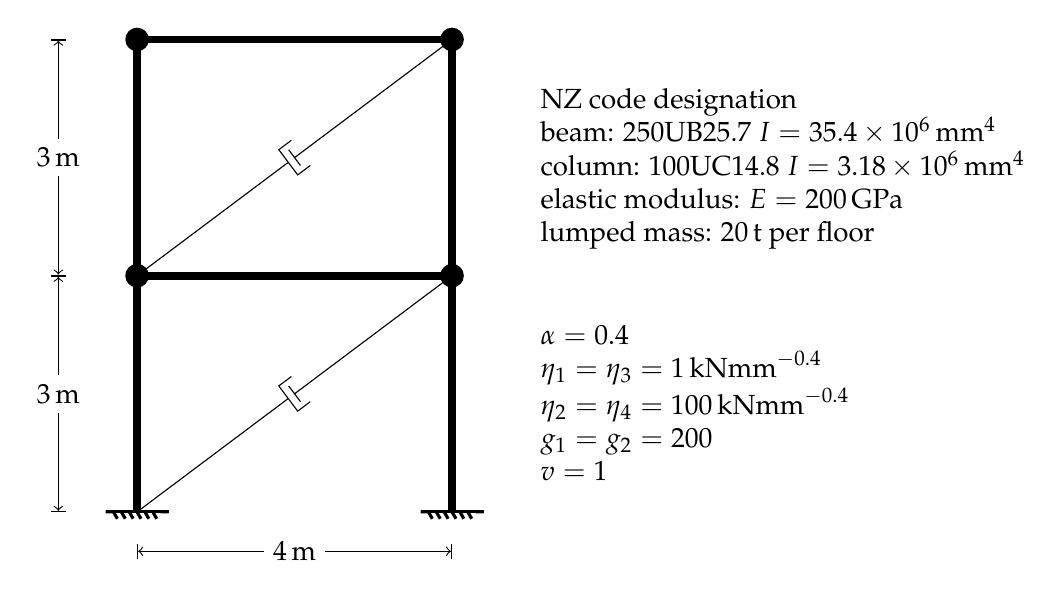
\begin{tikzpicture}
\draw[|<->|](0,-.5)--(4,-.5)node[midway,fill=white]{\SI{4}{\meter}};
\draw[|<->|](-1,0)--(-1,3)node[midway,fill=white]{\SI{3}{\meter}};
\draw[|<->|](-1,3)--(-1,6)node[midway,fill=white]{\SI{3}{\meter}};
\FixedSupport{0,0}
\FixedSupport{4,0}
\draw[line width=1mm](0,0)--(0,6)node[fill=black,circle,inner sep=0,minimum size=3mm]{}--(4,6)node[fill=black,circle,inner sep=0,minimum size=3mm]{}--(4,0);
\draw[line width=1mm](0,3)node[fill=black,circle,inner sep=0,minimum size=3mm]{}--(4,3)node[fill=black,circle,inner sep=0,minimum size=3mm]{};
\node[anchor=north west,align=left]at(5,5.5){NZ code designation\\beam: 250UB25.7 $I=\SI{35.4E6}{\milli\metre^4}$\\column: 100UC14.8 $I=\SI{3.18E6}{\milli\metre^4}$\\elastic modulus: $E=\SI{200}{\giga\pascal}$\\lumped mass: \SI{20}{\tonne} per floor};
\node[anchor=north west,align=left]at(5,2.5){$\alpha=0.4$\\$\eta_1=\eta_3=\SI{1}{\kilo\newton\milli\meter^{-0.4}}$\\$\eta_2=\eta_4=\SI{100}{\kilo\newton\milli\meter^{-0.4}}$\\$g_1=g_2=200$\\$v=1$};
\begin{scope}[rotate=36.8699]
\draw(0,0)--(2.4,0)(2.6,.2)--(2.4,.2)--(2.4,-.2)--(2.6,-.2)(2.5,.125)--(2.5,-.125)(2.5,0)--(5,0);
\end{scope}
\begin{scope}[rotate around={36.8699:(0,3)}]
\draw(0,0+3)--(2.4,0+3)(2.6,.2+3)--(2.4,.2+3)--(2.4,-.2+3)--(2.6,-.2+3)(2.5,.125+3)--(2.5,-.125+3)(2.5,0+3)--(5,0+3);
\end{scope}
\end{tikzpicture}
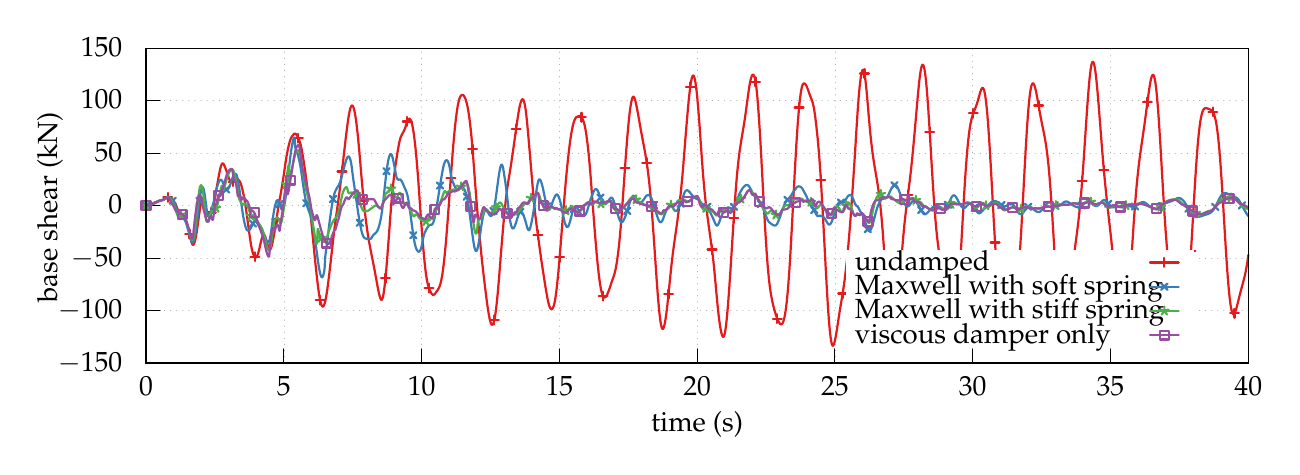
\begin{tikzpicture}[gnuplot]
%% generated with GNUPLOT 5.2p8 (Lua 5.3; terminal rev. Nov 2018, script rev. 108)
%% 08/29/2020 01:50:03
\path (0.000,0.000) rectangle (14.000,4.000);
\gpcolor{color=gp lt color axes}
\gpsetlinetype{gp lt axes}
\gpsetdashtype{gp dt axes}
\gpsetlinewidth{0.50}
\draw[gp path] (0.000,0.000)--(13.999,0.000);
\gpcolor{color=gp lt color border}
\gpsetlinetype{gp lt border}
\gpsetdashtype{gp dt solid}
\gpsetlinewidth{1.00}
\draw[gp path] (0.000,0.000)--(0.180,0.000);
\node[gp node right] at (-0.184,0.000) {$-150$};
\gpcolor{color=gp lt color axes}
\gpsetlinetype{gp lt axes}
\gpsetdashtype{gp dt axes}
\gpsetlinewidth{0.50}
\draw[gp path] (0.000,0.667)--(8.887,0.667);
\draw[gp path] (13.299,0.667)--(13.999,0.667);
\gpcolor{color=gp lt color border}
\gpsetlinetype{gp lt border}
\gpsetdashtype{gp dt solid}
\gpsetlinewidth{1.00}
\draw[gp path] (0.000,0.667)--(0.180,0.667);
\node[gp node right] at (-0.184,0.667) {$-100$};
\gpcolor{color=gp lt color axes}
\gpsetlinetype{gp lt axes}
\gpsetdashtype{gp dt axes}
\gpsetlinewidth{0.50}
\draw[gp path] (0.000,1.333)--(8.887,1.333);
\draw[gp path] (13.299,1.333)--(13.999,1.333);
\gpcolor{color=gp lt color border}
\gpsetlinetype{gp lt border}
\gpsetdashtype{gp dt solid}
\gpsetlinewidth{1.00}
\draw[gp path] (0.000,1.333)--(0.180,1.333);
\node[gp node right] at (-0.184,1.333) {$-50$};
\gpcolor{color=gp lt color axes}
\gpsetlinetype{gp lt axes}
\gpsetdashtype{gp dt axes}
\gpsetlinewidth{0.50}
\draw[gp path] (0.000,2.000)--(13.999,2.000);
\gpcolor{color=gp lt color border}
\gpsetlinetype{gp lt border}
\gpsetdashtype{gp dt solid}
\gpsetlinewidth{1.00}
\draw[gp path] (0.000,2.000)--(0.180,2.000);
\node[gp node right] at (-0.184,2.000) {$0$};
\gpcolor{color=gp lt color axes}
\gpsetlinetype{gp lt axes}
\gpsetdashtype{gp dt axes}
\gpsetlinewidth{0.50}
\draw[gp path] (0.000,2.666)--(13.999,2.666);
\gpcolor{color=gp lt color border}
\gpsetlinetype{gp lt border}
\gpsetdashtype{gp dt solid}
\gpsetlinewidth{1.00}
\draw[gp path] (0.000,2.666)--(0.180,2.666);
\node[gp node right] at (-0.184,2.666) {$50$};
\gpcolor{color=gp lt color axes}
\gpsetlinetype{gp lt axes}
\gpsetdashtype{gp dt axes}
\gpsetlinewidth{0.50}
\draw[gp path] (0.000,3.333)--(13.999,3.333);
\gpcolor{color=gp lt color border}
\gpsetlinetype{gp lt border}
\gpsetdashtype{gp dt solid}
\gpsetlinewidth{1.00}
\draw[gp path] (0.000,3.333)--(0.180,3.333);
\node[gp node right] at (-0.184,3.333) {$100$};
\gpcolor{color=gp lt color axes}
\gpsetlinetype{gp lt axes}
\gpsetdashtype{gp dt axes}
\gpsetlinewidth{0.50}
\draw[gp path] (0.000,3.999)--(13.999,3.999);
\gpcolor{color=gp lt color border}
\gpsetlinetype{gp lt border}
\gpsetdashtype{gp dt solid}
\gpsetlinewidth{1.00}
\draw[gp path] (0.000,3.999)--(0.180,3.999);
\node[gp node right] at (-0.184,3.999) {$150$};
\gpcolor{color=gp lt color axes}
\gpsetlinetype{gp lt axes}
\gpsetdashtype{gp dt axes}
\gpsetlinewidth{0.50}
\draw[gp path] (0.000,0.000)--(0.000,3.999);
\gpcolor{color=gp lt color border}
\gpsetlinetype{gp lt border}
\gpsetdashtype{gp dt solid}
\gpsetlinewidth{1.00}
\draw[gp path] (0.000,0.000)--(0.000,0.180);
\node[gp node center] at (0.000,-0.308) {$0$};
\gpcolor{color=gp lt color axes}
\gpsetlinetype{gp lt axes}
\gpsetdashtype{gp dt axes}
\gpsetlinewidth{0.50}
\draw[gp path] (1.750,0.000)--(1.750,3.999);
\gpcolor{color=gp lt color border}
\gpsetlinetype{gp lt border}
\gpsetdashtype{gp dt solid}
\gpsetlinewidth{1.00}
\draw[gp path] (1.750,0.000)--(1.750,0.180);
\node[gp node center] at (1.750,-0.308) {$5$};
\gpcolor{color=gp lt color axes}
\gpsetlinetype{gp lt axes}
\gpsetdashtype{gp dt axes}
\gpsetlinewidth{0.50}
\draw[gp path] (3.500,0.000)--(3.500,3.999);
\gpcolor{color=gp lt color border}
\gpsetlinetype{gp lt border}
\gpsetdashtype{gp dt solid}
\gpsetlinewidth{1.00}
\draw[gp path] (3.500,0.000)--(3.500,0.180);
\node[gp node center] at (3.500,-0.308) {$10$};
\gpcolor{color=gp lt color axes}
\gpsetlinetype{gp lt axes}
\gpsetdashtype{gp dt axes}
\gpsetlinewidth{0.50}
\draw[gp path] (5.250,0.000)--(5.250,3.999);
\gpcolor{color=gp lt color border}
\gpsetlinetype{gp lt border}
\gpsetdashtype{gp dt solid}
\gpsetlinewidth{1.00}
\draw[gp path] (5.250,0.000)--(5.250,0.180);
\node[gp node center] at (5.250,-0.308) {$15$};
\gpcolor{color=gp lt color axes}
\gpsetlinetype{gp lt axes}
\gpsetdashtype{gp dt axes}
\gpsetlinewidth{0.50}
\draw[gp path] (7.000,0.000)--(7.000,3.999);
\gpcolor{color=gp lt color border}
\gpsetlinetype{gp lt border}
\gpsetdashtype{gp dt solid}
\gpsetlinewidth{1.00}
\draw[gp path] (7.000,0.000)--(7.000,0.180);
\node[gp node center] at (7.000,-0.308) {$20$};
\gpcolor{color=gp lt color axes}
\gpsetlinetype{gp lt axes}
\gpsetdashtype{gp dt axes}
\gpsetlinewidth{0.50}
\draw[gp path] (8.749,0.000)--(8.749,3.999);
\gpcolor{color=gp lt color border}
\gpsetlinetype{gp lt border}
\gpsetdashtype{gp dt solid}
\gpsetlinewidth{1.00}
\draw[gp path] (8.749,0.000)--(8.749,0.180);
\node[gp node center] at (8.749,-0.308) {$25$};
\gpcolor{color=gp lt color axes}
\gpsetlinetype{gp lt axes}
\gpsetdashtype{gp dt axes}
\gpsetlinewidth{0.50}
\draw[gp path] (10.499,0.000)--(10.499,0.200);
\draw[gp path] (10.499,1.432)--(10.499,3.999);
\gpcolor{color=gp lt color border}
\gpsetlinetype{gp lt border}
\gpsetdashtype{gp dt solid}
\gpsetlinewidth{1.00}
\draw[gp path] (10.499,0.000)--(10.499,0.180);
\node[gp node center] at (10.499,-0.308) {$30$};
\gpcolor{color=gp lt color axes}
\gpsetlinetype{gp lt axes}
\gpsetdashtype{gp dt axes}
\gpsetlinewidth{0.50}
\draw[gp path] (12.249,0.000)--(12.249,0.200);
\draw[gp path] (12.249,1.432)--(12.249,3.999);
\gpcolor{color=gp lt color border}
\gpsetlinetype{gp lt border}
\gpsetdashtype{gp dt solid}
\gpsetlinewidth{1.00}
\draw[gp path] (12.249,0.000)--(12.249,0.180);
\node[gp node center] at (12.249,-0.308) {$35$};
\gpcolor{color=gp lt color axes}
\gpsetlinetype{gp lt axes}
\gpsetdashtype{gp dt axes}
\gpsetlinewidth{0.50}
\draw[gp path] (13.999,0.000)--(13.999,3.999);
\gpcolor{color=gp lt color border}
\gpsetlinetype{gp lt border}
\gpsetdashtype{gp dt solid}
\gpsetlinewidth{1.00}
\draw[gp path] (13.999,0.000)--(13.999,0.180);
\node[gp node center] at (13.999,-0.308) {$40$};
\draw[gp path] (0.000,3.999)--(0.000,0.000)--(13.999,0.000)--(13.999,3.999)--cycle;
\node[gp node center,rotate=-270] at (-1.212,1.999) {base shear (\si{\kilo\newton})};
\node[gp node center] at (6.999,-0.769) {time (\si{\second})};
\gpcolor{rgb color={0.894,0.102,0.110}}
\gpsetlinewidth{2.00}
\draw[gp path] (0.000,2.000)--(0.003,2.000)--(0.007,2.000)--(0.010,2.000)--(0.014,2.000)%
  --(0.017,2.000)--(0.021,2.000)--(0.024,2.001)--(0.028,2.001)--(0.031,2.002)--(0.035,2.002)%
  --(0.038,2.003)--(0.042,2.004)--(0.045,2.004)--(0.049,2.005)--(0.052,2.006)--(0.056,2.007)%
  --(0.059,2.008)--(0.063,2.009)--(0.066,2.011)--(0.070,2.012)--(0.073,2.013)--(0.077,2.014)%
  --(0.080,2.016)--(0.084,2.017)--(0.087,2.018)--(0.091,2.020)--(0.094,2.021)--(0.098,2.023)%
  --(0.101,2.025)--(0.105,2.027)--(0.108,2.028)--(0.112,2.030)--(0.115,2.032)--(0.119,2.034)%
  --(0.122,2.036)--(0.126,2.037)--(0.129,2.039)--(0.133,2.041)--(0.136,2.042)--(0.140,2.044)%
  --(0.143,2.045)--(0.147,2.047)--(0.150,2.049)--(0.154,2.050)--(0.157,2.052)--(0.161,2.054)%
  --(0.164,2.055)--(0.168,2.057)--(0.171,2.059)--(0.175,2.060)--(0.178,2.061)--(0.182,2.062)%
  --(0.185,2.063)--(0.189,2.064)--(0.192,2.065)--(0.196,2.066)--(0.199,2.067)--(0.203,2.068)%
  --(0.206,2.069)--(0.210,2.070)--(0.213,2.071)--(0.217,2.072)--(0.220,2.074)--(0.224,2.075)%
  --(0.227,2.077)--(0.231,2.079)--(0.234,2.081)--(0.238,2.083)--(0.241,2.085)--(0.245,2.087)%
  --(0.248,2.089)--(0.252,2.091)--(0.255,2.093)--(0.259,2.095)--(0.262,2.097)--(0.266,2.099)%
  --(0.269,2.101)--(0.273,2.103)--(0.276,2.104)--(0.280,2.105)--(0.283,2.106)--(0.287,2.107)%
  --(0.290,2.107)--(0.294,2.107)--(0.297,2.107)--(0.301,2.106)--(0.304,2.105)--(0.308,2.104)%
  --(0.311,2.102)--(0.315,2.100)--(0.318,2.097)--(0.322,2.094)--(0.325,2.091)--(0.329,2.087)%
  --(0.332,2.084)--(0.336,2.080)--(0.339,2.075)--(0.343,2.071)--(0.346,2.066)--(0.350,2.061)%
  --(0.353,2.056)--(0.357,2.051)--(0.360,2.045)--(0.364,2.039)--(0.367,2.032)--(0.371,2.026)%
  --(0.374,2.018)--(0.378,2.011)--(0.381,2.003)--(0.385,1.995)--(0.388,1.986)--(0.392,1.977)%
  --(0.395,1.969)--(0.399,1.960)--(0.402,1.951)--(0.406,1.942)--(0.409,1.934)--(0.413,1.925)%
  --(0.416,1.918)--(0.420,1.911)--(0.423,1.905)--(0.427,1.899)--(0.430,1.895)--(0.434,1.890)%
  --(0.437,1.887)--(0.441,1.884)--(0.444,1.881)--(0.448,1.879)--(0.451,1.877)--(0.455,1.875)%
  --(0.458,1.873)--(0.462,1.871)--(0.465,1.869)--(0.469,1.867)--(0.472,1.865)--(0.476,1.863)%
  --(0.479,1.860)--(0.483,1.856)--(0.486,1.852)--(0.490,1.847)--(0.493,1.841)--(0.497,1.835)%
  --(0.500,1.827)--(0.504,1.819)--(0.507,1.810)--(0.511,1.800)--(0.514,1.789)--(0.518,1.777)%
  --(0.521,1.765)--(0.525,1.753)--(0.528,1.740)--(0.532,1.727)--(0.535,1.713)--(0.539,1.699)%
  --(0.542,1.685)--(0.546,1.670)--(0.549,1.656)--(0.553,1.640)--(0.556,1.625)--(0.560,1.610)%
  --(0.563,1.594)--(0.567,1.578)--(0.570,1.563)--(0.574,1.549)--(0.577,1.536)--(0.581,1.525)%
  --(0.584,1.516)--(0.588,1.510)--(0.591,1.505)--(0.595,1.503)--(0.598,1.502)--(0.602,1.504)%
  --(0.605,1.508)--(0.609,1.513)--(0.612,1.521)--(0.616,1.530)--(0.619,1.541)--(0.623,1.554)%
  --(0.626,1.568)--(0.630,1.585)--(0.633,1.602)--(0.637,1.622)--(0.640,1.642)--(0.644,1.664)%
  --(0.647,1.687)--(0.651,1.711)--(0.654,1.735)--(0.658,1.760)--(0.661,1.785)--(0.665,1.811)%
  --(0.668,1.837)--(0.672,1.862)--(0.675,1.887)--(0.679,1.911)--(0.682,1.935)--(0.686,1.957)%
  --(0.689,1.979)--(0.693,1.999)--(0.696,2.017)--(0.700,2.034)--(0.703,2.049)--(0.707,2.062)%
  --(0.710,2.073)--(0.714,2.082)--(0.717,2.089)--(0.721,2.093)--(0.724,2.094)--(0.728,2.093)%
  --(0.731,2.090)--(0.735,2.084)--(0.738,2.075)--(0.742,2.064)--(0.745,2.050)--(0.749,2.035)%
  --(0.752,2.017)--(0.756,1.998)--(0.759,1.977)--(0.763,1.957)--(0.766,1.938)--(0.770,1.921)%
  --(0.773,1.905)--(0.777,1.892)--(0.780,1.881)--(0.784,1.873)--(0.787,1.866)--(0.791,1.862)%
  --(0.794,1.860)--(0.798,1.859)--(0.801,1.860)--(0.805,1.863)--(0.808,1.867)--(0.812,1.872)%
  --(0.815,1.879)--(0.819,1.886)--(0.822,1.894)--(0.826,1.903)--(0.829,1.913)--(0.833,1.922)%
  --(0.836,1.932)--(0.840,1.942)--(0.843,1.951)--(0.847,1.961)--(0.850,1.971)--(0.854,1.982)%
  --(0.857,1.996)--(0.861,2.011)--(0.864,2.028)--(0.868,2.046)--(0.871,2.065)--(0.875,2.086)%
  --(0.878,2.107)--(0.882,2.128)--(0.885,2.150)--(0.889,2.171)--(0.892,2.192)--(0.896,2.212)%
  --(0.899,2.232)--(0.903,2.253)--(0.906,2.273)--(0.910,2.293)--(0.913,2.314)--(0.917,2.334)%
  --(0.920,2.354)--(0.924,2.374)--(0.927,2.393)--(0.931,2.412)--(0.934,2.429)--(0.938,2.446)%
  --(0.941,2.462)--(0.945,2.476)--(0.948,2.489)--(0.952,2.501)--(0.955,2.511)--(0.959,2.519)%
  --(0.962,2.526)--(0.966,2.531)--(0.969,2.535)--(0.973,2.536)--(0.976,2.535)--(0.980,2.533)%
  --(0.983,2.530)--(0.987,2.525)--(0.990,2.519)--(0.994,2.511)--(0.997,2.504)--(1.001,2.495)%
  --(1.004,2.487)--(1.008,2.478)--(1.011,2.468)--(1.015,2.459)--(1.018,2.449)--(1.022,2.439)%
  --(1.025,2.429)--(1.029,2.419)--(1.032,2.409)--(1.036,2.399)--(1.039,2.389)--(1.043,2.379)%
  --(1.046,2.369)--(1.050,2.359)--(1.053,2.349)--(1.057,2.339)--(1.060,2.331)--(1.064,2.323)%
  --(1.067,2.317)--(1.071,2.311)--(1.074,2.306)--(1.078,2.303)--(1.081,2.300)--(1.085,2.299)%
  --(1.088,2.298)--(1.092,2.298)--(1.095,2.298)--(1.099,2.299)--(1.102,2.301)--(1.106,2.303)%
  --(1.109,2.305)--(1.113,2.307)--(1.116,2.309)--(1.120,2.312)--(1.123,2.314)--(1.127,2.318)%
  --(1.130,2.321)--(1.134,2.325)--(1.137,2.329)--(1.141,2.333)--(1.144,2.336)--(1.148,2.339)%
  --(1.151,2.341)--(1.155,2.342)--(1.158,2.342)--(1.162,2.340)--(1.165,2.337)--(1.169,2.333)%
  --(1.172,2.329)--(1.176,2.325)--(1.179,2.321)--(1.183,2.317)--(1.186,2.313)--(1.190,2.308)%
  --(1.193,2.302)--(1.197,2.295)--(1.200,2.288)--(1.204,2.278)--(1.207,2.268)--(1.211,2.256)%
  --(1.214,2.243)--(1.218,2.230)--(1.221,2.217)--(1.225,2.203)--(1.228,2.188)--(1.232,2.173)%
  --(1.235,2.157)--(1.239,2.140)--(1.242,2.123)--(1.246,2.105)--(1.249,2.085)--(1.253,2.065)%
  --(1.256,2.044)--(1.260,2.022)--(1.263,2.000)--(1.267,1.976)--(1.270,1.952)--(1.274,1.928)%
  --(1.277,1.903)--(1.281,1.878)--(1.284,1.852)--(1.288,1.827)--(1.291,1.801)--(1.295,1.776)%
  --(1.298,1.750)--(1.302,1.724)--(1.305,1.698)--(1.309,1.673)--(1.312,1.647)--(1.316,1.622)%
  --(1.319,1.597)--(1.323,1.573)--(1.326,1.549)--(1.330,1.527)--(1.333,1.505)--(1.337,1.485)%
  --(1.340,1.467)--(1.344,1.450)--(1.347,1.434)--(1.351,1.420)--(1.354,1.407)--(1.358,1.396)%
  --(1.361,1.386)--(1.365,1.377)--(1.368,1.370)--(1.372,1.363)--(1.375,1.358)--(1.379,1.353)%
  --(1.382,1.350)--(1.386,1.347)--(1.389,1.344)--(1.393,1.343)--(1.396,1.343)--(1.400,1.345)%
  --(1.403,1.348)--(1.407,1.352)--(1.410,1.358)--(1.414,1.365)--(1.417,1.374)--(1.421,1.383)%
  --(1.424,1.394)--(1.428,1.405)--(1.431,1.418)--(1.435,1.432)--(1.438,1.446)--(1.442,1.461)%
  --(1.445,1.477)--(1.449,1.492)--(1.452,1.508)--(1.456,1.523)--(1.459,1.538)--(1.463,1.552)%
  --(1.466,1.566)--(1.470,1.579)--(1.473,1.591)--(1.477,1.601)--(1.480,1.610)--(1.484,1.618)%
  --(1.487,1.624)--(1.491,1.628)--(1.494,1.630)--(1.498,1.630)--(1.501,1.628)--(1.505,1.625)%
  --(1.508,1.619)--(1.512,1.611)--(1.515,1.602)--(1.519,1.591)--(1.522,1.579)--(1.526,1.566)%
  --(1.529,1.554)--(1.533,1.542)--(1.536,1.530)--(1.540,1.518)--(1.543,1.506)--(1.547,1.495)%
  --(1.550,1.484)--(1.554,1.473)--(1.557,1.464)--(1.561,1.456)--(1.564,1.449)--(1.568,1.445)%
  --(1.571,1.442)--(1.575,1.442)--(1.578,1.444)--(1.582,1.448)--(1.585,1.454)--(1.589,1.462)%
  --(1.592,1.472)--(1.596,1.484)--(1.599,1.497)--(1.603,1.512)--(1.606,1.528)--(1.610,1.545)%
  --(1.613,1.563)--(1.617,1.581)--(1.620,1.600)--(1.624,1.620)--(1.627,1.639)--(1.631,1.658)%
  --(1.634,1.678)--(1.638,1.698)--(1.641,1.718)--(1.645,1.739)--(1.648,1.762)--(1.652,1.785)%
  --(1.655,1.809)--(1.659,1.833)--(1.662,1.858)--(1.666,1.882)--(1.669,1.907)--(1.673,1.932)%
  --(1.676,1.955)--(1.680,1.979)--(1.683,2.001)--(1.687,2.022)--(1.690,2.041)--(1.694,2.060)%
  --(1.697,2.077)--(1.701,2.095)--(1.704,2.113)--(1.708,2.132)--(1.711,2.152)--(1.715,2.172)%
  --(1.718,2.193)--(1.722,2.214)--(1.725,2.235)--(1.729,2.257)--(1.732,2.278)--(1.736,2.300)%
  --(1.739,2.322)--(1.743,2.344)--(1.746,2.367)--(1.750,2.390)--(1.753,2.414)--(1.757,2.438)%
  --(1.760,2.462)--(1.764,2.487)--(1.767,2.511)--(1.771,2.534)--(1.774,2.558)--(1.778,2.581)%
  --(1.781,2.603)--(1.785,2.624)--(1.788,2.644)--(1.792,2.663)--(1.795,2.681)--(1.799,2.699)%
  --(1.802,2.715)--(1.806,2.732)--(1.809,2.747)--(1.813,2.762)--(1.816,2.776)--(1.820,2.790)%
  --(1.823,2.803)--(1.827,2.815)--(1.830,2.826)--(1.834,2.837)--(1.837,2.846)--(1.841,2.854)%
  --(1.844,2.862)--(1.848,2.868)--(1.851,2.873)--(1.855,2.878)--(1.858,2.884)--(1.862,2.888)%
  --(1.865,2.893)--(1.869,2.897)--(1.872,2.901)--(1.876,2.905)--(1.879,2.908)--(1.883,2.910)%
  --(1.886,2.912)--(1.890,2.913)--(1.893,2.913)--(1.897,2.913)--(1.900,2.911)--(1.904,2.908)%
  --(1.907,2.905)--(1.911,2.900)--(1.914,2.895)--(1.918,2.889)--(1.921,2.883)--(1.925,2.877)%
  --(1.928,2.870)--(1.932,2.863)--(1.935,2.855)--(1.939,2.848)--(1.942,2.839)--(1.946,2.831)%
  --(1.949,2.821)--(1.953,2.811)--(1.956,2.800)--(1.960,2.788)--(1.963,2.775)--(1.967,2.762)%
  --(1.970,2.746)--(1.974,2.730)--(1.977,2.712)--(1.981,2.693)--(1.984,2.674)--(1.988,2.653)%
  --(1.991,2.632)--(1.995,2.610)--(1.998,2.588)--(2.002,2.566)--(2.005,2.544)--(2.009,2.521)%
  --(2.012,2.497)--(2.016,2.473)--(2.019,2.449)--(2.023,2.424)--(2.026,2.399)--(2.030,2.373)%
  --(2.033,2.347)--(2.037,2.321)--(2.040,2.294)--(2.044,2.267)--(2.047,2.240)--(2.051,2.213)%
  --(2.054,2.185)--(2.058,2.158)--(2.061,2.129)--(2.065,2.101)--(2.068,2.072)--(2.072,2.043)%
  --(2.075,2.013)--(2.079,1.983)--(2.082,1.952)--(2.086,1.921)--(2.089,1.888)--(2.093,1.856)%
  --(2.096,1.822)--(2.100,1.788)--(2.103,1.753)--(2.107,1.717)--(2.110,1.682)--(2.114,1.646)%
  --(2.117,1.611)--(2.121,1.575)--(2.124,1.540)--(2.128,1.504)--(2.131,1.469)--(2.135,1.433)%
  --(2.138,1.398)--(2.142,1.362)--(2.145,1.327)--(2.149,1.293)--(2.152,1.259)--(2.156,1.225)%
  --(2.159,1.192)--(2.163,1.159)--(2.166,1.128)--(2.170,1.096)--(2.173,1.066)--(2.177,1.036)%
  --(2.180,1.006)--(2.184,0.978)--(2.187,0.951)--(2.191,0.925)--(2.194,0.900)--(2.198,0.876)%
  --(2.201,0.855)--(2.205,0.834)--(2.208,0.815)--(2.212,0.798)--(2.215,0.782)--(2.219,0.768)%
  --(2.222,0.756)--(2.226,0.745)--(2.229,0.736)--(2.233,0.729)--(2.236,0.724)--(2.240,0.720)%
  --(2.243,0.718)--(2.247,0.718)--(2.250,0.720)--(2.254,0.723)--(2.257,0.728)--(2.261,0.734)%
  --(2.264,0.743)--(2.268,0.753)--(2.271,0.764)--(2.275,0.778)--(2.278,0.793)--(2.282,0.809)%
  --(2.285,0.828)--(2.289,0.847)--(2.292,0.868)--(2.296,0.890)--(2.299,0.914)--(2.303,0.938)%
  --(2.306,0.964)--(2.310,0.990)--(2.313,1.017)--(2.317,1.045)--(2.320,1.073)--(2.324,1.101)%
  --(2.327,1.131)--(2.331,1.160)--(2.334,1.190)--(2.338,1.221)--(2.341,1.251)--(2.345,1.282)%
  --(2.348,1.313)--(2.352,1.344)--(2.355,1.375)--(2.359,1.406)--(2.362,1.437)--(2.366,1.468)%
  --(2.369,1.499)--(2.373,1.530)--(2.376,1.560)--(2.380,1.591)--(2.383,1.620)--(2.387,1.650)%
  --(2.390,1.678)--(2.394,1.707)--(2.397,1.734)--(2.401,1.761)--(2.404,1.787)--(2.408,1.813)%
  --(2.411,1.838)--(2.415,1.863)--(2.418,1.888)--(2.422,1.914)--(2.425,1.939)--(2.429,1.965)%
  --(2.432,1.990)--(2.436,2.015)--(2.439,2.041)--(2.443,2.067)--(2.446,2.092)--(2.450,2.118)%
  --(2.453,2.144)--(2.457,2.171)--(2.460,2.198)--(2.464,2.226)--(2.467,2.255)--(2.471,2.283)%
  --(2.474,2.313)--(2.478,2.342)--(2.481,2.373)--(2.485,2.403)--(2.488,2.433)--(2.492,2.464)%
  --(2.495,2.494)--(2.499,2.525)--(2.502,2.555)--(2.506,2.585)--(2.509,2.616)--(2.513,2.646)%
  --(2.516,2.676)--(2.520,2.707)--(2.523,2.738)--(2.527,2.768)--(2.530,2.798)--(2.534,2.829)%
  --(2.537,2.859)--(2.541,2.888)--(2.544,2.917)--(2.548,2.946)--(2.551,2.974)--(2.555,3.002)%
  --(2.558,3.028)--(2.562,3.054)--(2.565,3.079)--(2.569,3.102)--(2.572,3.124)--(2.576,3.145)%
  --(2.579,3.164)--(2.583,3.182)--(2.586,3.199)--(2.590,3.214)--(2.593,3.227)--(2.597,3.239)%
  --(2.600,3.249)--(2.604,3.257)--(2.607,3.264)--(2.611,3.268)--(2.614,3.270)--(2.618,3.271)%
  --(2.621,3.269)--(2.625,3.265)--(2.628,3.260)--(2.632,3.253)--(2.635,3.244)--(2.639,3.233)%
  --(2.642,3.221)--(2.646,3.207)--(2.649,3.191)--(2.653,3.174)--(2.656,3.155)--(2.660,3.134)%
  --(2.663,3.111)--(2.667,3.088)--(2.670,3.062)--(2.674,3.035)--(2.677,3.006)--(2.681,2.976)%
  --(2.684,2.944)--(2.688,2.911)--(2.691,2.877)--(2.695,2.842)--(2.698,2.806)--(2.702,2.769)%
  --(2.705,2.731)--(2.709,2.692)--(2.712,2.652)--(2.716,2.612)--(2.719,2.571)--(2.723,2.530)%
  --(2.726,2.488)--(2.730,2.447)--(2.733,2.405)--(2.737,2.364)--(2.740,2.323)--(2.744,2.283)%
  --(2.747,2.244)--(2.751,2.205)--(2.754,2.167)--(2.758,2.130)--(2.761,2.094)--(2.765,2.058)%
  --(2.768,2.024)--(2.772,1.991)--(2.775,1.959)--(2.779,1.928)--(2.782,1.897)--(2.786,1.868)%
  --(2.789,1.839)--(2.793,1.812)--(2.796,1.784)--(2.800,1.758)--(2.803,1.732)--(2.807,1.707)%
  --(2.810,1.682)--(2.814,1.659)--(2.817,1.636)--(2.821,1.614)--(2.824,1.593)--(2.828,1.572)%
  --(2.831,1.552)--(2.835,1.532)--(2.838,1.513)--(2.842,1.494)--(2.845,1.476)--(2.849,1.457)%
  --(2.852,1.439)--(2.856,1.421)--(2.859,1.403)--(2.863,1.385)--(2.866,1.367)--(2.870,1.349)%
  --(2.873,1.332)--(2.877,1.314)--(2.880,1.296)--(2.884,1.279)--(2.887,1.261)--(2.891,1.243)%
  --(2.894,1.225)--(2.898,1.207)--(2.901,1.189)--(2.905,1.170)--(2.908,1.151)--(2.912,1.132)%
  --(2.915,1.113)--(2.919,1.094)--(2.922,1.074)--(2.926,1.055)--(2.929,1.035)--(2.933,1.016)%
  --(2.936,0.997)--(2.940,0.978)--(2.943,0.959)--(2.947,0.941)--(2.950,0.924)--(2.954,0.907)%
  --(2.957,0.891)--(2.961,0.876)--(2.964,0.862)--(2.968,0.850)--(2.971,0.838)--(2.975,0.827)%
  --(2.978,0.818)--(2.982,0.811)--(2.985,0.806)--(2.989,0.803)--(2.992,0.803)--(2.996,0.805)%
  --(2.999,0.811)--(3.003,0.819)--(3.006,0.830)--(3.010,0.843)--(3.013,0.860)--(3.017,0.879)%
  --(3.020,0.900)--(3.024,0.925)--(3.027,0.951)--(3.031,0.980)--(3.034,1.011)--(3.038,1.044)%
  --(3.041,1.078)--(3.045,1.115)--(3.048,1.153)--(3.052,1.193)--(3.055,1.234)--(3.059,1.276)%
  --(3.062,1.319)--(3.066,1.363)--(3.069,1.408)--(3.073,1.454)--(3.076,1.501)--(3.080,1.548)%
  --(3.083,1.595)--(3.087,1.643)--(3.090,1.691)--(3.094,1.738)--(3.097,1.786)--(3.101,1.833)%
  --(3.104,1.879)--(3.108,1.925)--(3.111,1.970)--(3.115,2.014)--(3.118,2.056)--(3.122,2.097)%
  --(3.125,2.137)--(3.129,2.174)--(3.132,2.210)--(3.136,2.243)--(3.139,2.275)--(3.143,2.306)%
  --(3.146,2.336)--(3.150,2.366)--(3.153,2.394)--(3.157,2.422)--(3.160,2.450)--(3.164,2.476)%
  --(3.167,2.501)--(3.171,2.526)--(3.174,2.550)--(3.178,2.574)--(3.181,2.597)--(3.185,2.619)%
  --(3.188,2.641)--(3.192,2.663)--(3.195,2.684)--(3.199,2.704)--(3.202,2.725)--(3.206,2.744)%
  --(3.209,2.763)--(3.213,2.781)--(3.216,2.798)--(3.220,2.814)--(3.223,2.829)--(3.227,2.842)%
  --(3.230,2.854)--(3.234,2.864)--(3.237,2.874)--(3.241,2.882)--(3.244,2.890)--(3.248,2.897)%
  --(3.251,2.904)--(3.255,2.910)--(3.258,2.917)--(3.262,2.923)--(3.265,2.929)--(3.269,2.935)%
  --(3.272,2.941)--(3.276,2.948)--(3.279,2.956)--(3.283,2.964)--(3.286,2.973)--(3.290,2.982)%
  --(3.293,2.992)--(3.297,3.003)--(3.300,3.014)--(3.304,3.026)--(3.307,3.037)--(3.311,3.048)%
  --(3.314,3.059)--(3.318,3.069)--(3.321,3.078)--(3.325,3.086)--(3.328,3.092)--(3.332,3.097)%
  --(3.335,3.100)--(3.339,3.102)--(3.342,3.102)--(3.346,3.102)--(3.349,3.101)--(3.353,3.098)%
  --(3.356,3.094)--(3.360,3.089)--(3.363,3.083)--(3.367,3.075)--(3.370,3.066)--(3.374,3.055)%
  --(3.377,3.042)--(3.381,3.027)--(3.384,3.010)--(3.388,2.992)--(3.391,2.971)--(3.395,2.950)%
  --(3.398,2.927)--(3.402,2.903)--(3.405,2.877)--(3.409,2.850)--(3.412,2.822)--(3.416,2.792)%
  --(3.419,2.760)--(3.423,2.727)--(3.426,2.693)--(3.430,2.657)--(3.433,2.620)--(3.437,2.581)%
  --(3.440,2.540)--(3.444,2.499)--(3.447,2.455)--(3.451,2.410)--(3.454,2.364)--(3.458,2.317)%
  --(3.461,2.269)--(3.465,2.220)--(3.468,2.170)--(3.472,2.120)--(3.475,2.070)--(3.479,2.020)%
  --(3.482,1.970)--(3.486,1.921)--(3.489,1.872)--(3.493,1.823)--(3.496,1.776)--(3.500,1.730)%
  --(3.503,1.684)--(3.507,1.639)--(3.510,1.595)--(3.514,1.552)--(3.517,1.509)--(3.521,1.468)%
  --(3.524,1.427)--(3.528,1.388)--(3.531,1.351)--(3.535,1.314)--(3.538,1.280)--(3.542,1.247)%
  --(3.545,1.215)--(3.549,1.185)--(3.552,1.157)--(3.556,1.131)--(3.559,1.106)--(3.563,1.084)%
  --(3.566,1.063)--(3.570,1.044)--(3.573,1.026)--(3.577,1.011)--(3.580,0.996)--(3.584,0.983)%
  --(3.587,0.972)--(3.591,0.961)--(3.594,0.951)--(3.598,0.942)--(3.601,0.933)--(3.605,0.925)%
  --(3.608,0.917)--(3.612,0.909)--(3.615,0.902)--(3.619,0.895)--(3.622,0.888)--(3.626,0.883)%
  --(3.629,0.878)--(3.633,0.874)--(3.636,0.871)--(3.640,0.868)--(3.643,0.866)--(3.647,0.865)%
  --(3.650,0.865)--(3.654,0.866)--(3.657,0.868)--(3.661,0.871)--(3.664,0.874)--(3.668,0.878)%
  --(3.671,0.882)--(3.675,0.887)--(3.678,0.892)--(3.682,0.896)--(3.685,0.901)--(3.689,0.906)%
  --(3.692,0.911)--(3.696,0.915)--(3.699,0.920)--(3.703,0.925)--(3.706,0.930)--(3.710,0.935)%
  --(3.713,0.941)--(3.717,0.948)--(3.720,0.955)--(3.724,0.963)--(3.727,0.971)--(3.731,0.981)%
  --(3.734,0.991)--(3.738,1.003)--(3.741,1.015)--(3.745,1.029)--(3.748,1.044)--(3.752,1.061)%
  --(3.755,1.079)--(3.759,1.098)--(3.762,1.120)--(3.766,1.142)--(3.769,1.167)--(3.773,1.193)%
  --(3.776,1.220)--(3.780,1.249)--(3.783,1.279)--(3.787,1.310)--(3.790,1.343)--(3.794,1.377)%
  --(3.797,1.412)--(3.801,1.448)--(3.804,1.486)--(3.808,1.524)--(3.811,1.564)--(3.815,1.606)%
  --(3.818,1.648)--(3.822,1.692)--(3.825,1.737)--(3.829,1.783)--(3.832,1.829)--(3.836,1.876)%
  --(3.839,1.924)--(3.843,1.971)--(3.846,2.019)--(3.850,2.067)--(3.853,2.114)--(3.857,2.162)%
  --(3.860,2.209)--(3.864,2.257)--(3.867,2.304)--(3.871,2.351)--(3.874,2.399)--(3.878,2.446)%
  --(3.881,2.493)--(3.885,2.540)--(3.888,2.586)--(3.892,2.632)--(3.895,2.677)--(3.899,2.720)%
  --(3.902,2.763)--(3.906,2.804)--(3.909,2.844)--(3.913,2.883)--(3.916,2.920)--(3.920,2.955)%
  --(3.923,2.990)--(3.927,3.023)--(3.930,3.054)--(3.934,3.085)--(3.937,3.114)--(3.941,3.142)%
  --(3.944,3.168)--(3.948,3.193)--(3.951,3.217)--(3.955,3.240)--(3.958,3.261)--(3.962,3.280)%
  --(3.965,3.298)--(3.969,3.314)--(3.972,3.329)--(3.976,3.342)--(3.979,3.354)--(3.983,3.364)%
  --(3.986,3.373)--(3.990,3.380)--(3.993,3.387)--(3.997,3.392)--(4.000,3.396)--(4.004,3.400)%
  --(4.007,3.402)--(4.011,3.404)--(4.014,3.405)--(4.018,3.406)--(4.021,3.405)--(4.025,3.404)%
  --(4.028,3.402)--(4.032,3.399)--(4.035,3.395)--(4.039,3.391)--(4.042,3.386)--(4.046,3.380)%
  --(4.049,3.373)--(4.053,3.365)--(4.056,3.356)--(4.060,3.347)--(4.063,3.336)--(4.067,3.325)%
  --(4.070,3.312)--(4.074,3.298)--(4.077,3.283)--(4.081,3.267)--(4.084,3.250)--(4.088,3.232)%
  --(4.091,3.212)--(4.095,3.191)--(4.098,3.169)--(4.102,3.146)--(4.105,3.121)--(4.109,3.095)%
  --(4.112,3.067)--(4.116,3.038)--(4.119,3.008)--(4.123,2.977)--(4.126,2.944)--(4.130,2.910)%
  --(4.133,2.874)--(4.137,2.836)--(4.140,2.797)--(4.144,2.757)--(4.147,2.714)--(4.151,2.671)%
  --(4.154,2.626)--(4.158,2.580)--(4.161,2.534)--(4.165,2.487)--(4.168,2.440)--(4.172,2.394)%
  --(4.175,2.347)--(4.179,2.301)--(4.182,2.255)--(4.186,2.209)--(4.189,2.164)--(4.193,2.119)%
  --(4.196,2.074)--(4.200,2.031)--(4.203,1.988)--(4.207,1.946)--(4.210,1.904)--(4.214,1.863)%
  --(4.217,1.823)--(4.221,1.783)--(4.224,1.744)--(4.228,1.705)--(4.231,1.667)--(4.235,1.629)%
  --(4.238,1.592)--(4.242,1.555)--(4.245,1.518)--(4.249,1.482)--(4.252,1.446)--(4.256,1.411)%
  --(4.259,1.377)--(4.263,1.343)--(4.266,1.309)--(4.270,1.276)--(4.273,1.244)--(4.277,1.212)%
  --(4.280,1.181)--(4.284,1.151)--(4.287,1.121)--(4.291,1.091)--(4.294,1.062)--(4.298,1.033)%
  --(4.301,1.003)--(4.305,0.974)--(4.308,0.946)--(4.312,0.917)--(4.315,0.889)--(4.319,0.861)%
  --(4.322,0.833)--(4.326,0.806)--(4.329,0.780)--(4.333,0.754)--(4.336,0.729)--(4.340,0.705)%
  --(4.343,0.682)--(4.347,0.659)--(4.350,0.637)--(4.354,0.616)--(4.357,0.597)--(4.361,0.579)%
  --(4.364,0.562)--(4.368,0.547)--(4.371,0.534)--(4.375,0.522)--(4.378,0.512)--(4.382,0.503)%
  --(4.385,0.496)--(4.389,0.491)--(4.392,0.488)--(4.396,0.486)--(4.399,0.487)--(4.403,0.489)%
  --(4.406,0.493)--(4.410,0.500)--(4.413,0.508)--(4.417,0.519)--(4.420,0.532)--(4.424,0.547)%
  --(4.427,0.563)--(4.431,0.583)--(4.434,0.604)--(4.438,0.627)--(4.441,0.652)--(4.445,0.679)%
  --(4.448,0.708)--(4.452,0.738)--(4.455,0.770)--(4.459,0.804)--(4.462,0.839)--(4.466,0.876)%
  --(4.469,0.914)--(4.473,0.953)--(4.476,0.994)--(4.480,1.036)--(4.483,1.078)--(4.487,1.122)%
  --(4.490,1.166)--(4.494,1.210)--(4.497,1.254)--(4.501,1.298)--(4.504,1.343)--(4.508,1.387)%
  --(4.511,1.431)--(4.515,1.474)--(4.518,1.517)--(4.522,1.560)--(4.525,1.602)--(4.529,1.643)%
  --(4.532,1.684)--(4.536,1.724)--(4.539,1.764)--(4.543,1.803)--(4.546,1.841)--(4.550,1.878)%
  --(4.553,1.914)--(4.557,1.950)--(4.560,1.984)--(4.564,2.018)--(4.567,2.050)--(4.571,2.081)%
  --(4.574,2.112)--(4.578,2.141)--(4.581,2.169)--(4.585,2.195)--(4.588,2.221)--(4.592,2.246)%
  --(4.595,2.269)--(4.599,2.292)--(4.602,2.314)--(4.606,2.336)--(4.609,2.357)--(4.613,2.379)%
  --(4.616,2.400)--(4.620,2.421)--(4.623,2.442)--(4.627,2.464)--(4.630,2.486)--(4.634,2.508)%
  --(4.637,2.531)--(4.641,2.554)--(4.644,2.577)--(4.648,2.601)--(4.651,2.625)--(4.655,2.649)%
  --(4.658,2.673)--(4.662,2.698)--(4.665,2.722)--(4.669,2.747)--(4.672,2.772)--(4.676,2.797)%
  --(4.679,2.822)--(4.683,2.848)--(4.686,2.874)--(4.690,2.899)--(4.693,2.925)--(4.697,2.950)%
  --(4.700,2.975)--(4.704,2.999)--(4.707,3.023)--(4.711,3.046)--(4.714,3.070)--(4.718,3.094)%
  --(4.721,3.117)--(4.725,3.140)--(4.728,3.162)--(4.732,3.184)--(4.735,3.204)--(4.739,3.224)%
  --(4.742,3.242)--(4.746,3.259)--(4.749,3.275)--(4.753,3.289)--(4.756,3.302)--(4.760,3.314)%
  --(4.763,3.324)--(4.767,3.332)--(4.770,3.339)--(4.774,3.345)--(4.777,3.348)--(4.781,3.350)%
  --(4.784,3.350)--(4.788,3.347)--(4.791,3.343)--(4.795,3.337)--(4.798,3.328)--(4.802,3.318)%
  --(4.805,3.305)--(4.809,3.290)--(4.812,3.273)--(4.816,3.253)--(4.819,3.232)--(4.823,3.207)%
  --(4.826,3.181)--(4.830,3.152)--(4.833,3.120)--(4.837,3.086)--(4.840,3.051)--(4.844,3.014)%
  --(4.847,2.976)--(4.851,2.938)--(4.854,2.898)--(4.858,2.858)--(4.861,2.818)--(4.865,2.778)%
  --(4.868,2.737)--(4.872,2.695)--(4.875,2.654)--(4.879,2.613)--(4.882,2.571)--(4.886,2.530)%
  --(4.889,2.488)--(4.893,2.446)--(4.896,2.405)--(4.900,2.363)--(4.903,2.322)--(4.907,2.280)%
  --(4.910,2.239)--(4.914,2.198)--(4.917,2.158)--(4.921,2.118)--(4.924,2.080)--(4.928,2.042)%
  --(4.931,2.006)--(4.935,1.971)--(4.938,1.937)--(4.942,1.904)--(4.945,1.873)--(4.949,1.843)%
  --(4.952,1.814)--(4.956,1.786)--(4.959,1.759)--(4.963,1.732)--(4.966,1.706)--(4.970,1.681)%
  --(4.973,1.655)--(4.977,1.630)--(4.980,1.604)--(4.984,1.579)--(4.987,1.553)--(4.991,1.527)%
  --(4.994,1.500)--(4.998,1.474)--(5.001,1.448)--(5.005,1.422)--(5.008,1.396)--(5.012,1.371)%
  --(5.015,1.346)--(5.019,1.321)--(5.022,1.297)--(5.026,1.274)--(5.029,1.251)--(5.033,1.228)%
  --(5.036,1.205)--(5.040,1.182)--(5.043,1.159)--(5.047,1.136)--(5.050,1.113)--(5.054,1.090)%
  --(5.057,1.067)--(5.061,1.044)--(5.064,1.022)--(5.068,1.000)--(5.071,0.978)--(5.075,0.957)%
  --(5.078,0.936)--(5.082,0.915)--(5.085,0.895)--(5.089,0.875)--(5.092,0.856)--(5.096,0.837)%
  --(5.099,0.819)--(5.103,0.802)--(5.106,0.785)--(5.110,0.770)--(5.113,0.756)--(5.117,0.743)%
  --(5.120,0.731)--(5.124,0.720)--(5.127,0.711)--(5.131,0.704)--(5.134,0.697)--(5.138,0.692)%
  --(5.141,0.688)--(5.145,0.685)--(5.148,0.684)--(5.152,0.684)--(5.155,0.685)--(5.159,0.688)%
  --(5.162,0.692)--(5.166,0.697)--(5.169,0.704)--(5.173,0.712)--(5.176,0.721)--(5.180,0.732)%
  --(5.183,0.745)--(5.187,0.759)--(5.190,0.775)--(5.194,0.794)--(5.197,0.814)--(5.201,0.836)%
  --(5.204,0.860)--(5.208,0.886)--(5.211,0.914)--(5.215,0.943)--(5.218,0.973)--(5.222,1.005)%
  --(5.225,1.038)--(5.229,1.072)--(5.232,1.107)--(5.236,1.144)--(5.239,1.181)--(5.243,1.220)%
  --(5.246,1.261)--(5.250,1.302)--(5.253,1.344)--(5.257,1.387)--(5.260,1.431)--(5.264,1.475)%
  --(5.267,1.519)--(5.271,1.563)--(5.274,1.608)--(5.278,1.652)--(5.281,1.696)--(5.285,1.739)%
  --(5.288,1.783)--(5.292,1.827)--(5.295,1.870)--(5.299,1.914)--(5.302,1.957)--(5.306,2.000)%
  --(5.309,2.043)--(5.313,2.086)--(5.316,2.128)--(5.320,2.170)--(5.323,2.211)--(5.327,2.252)%
  --(5.330,2.292)--(5.334,2.331)--(5.337,2.369)--(5.341,2.406)--(5.344,2.443)--(5.348,2.478)%
  --(5.351,2.513)--(5.355,2.547)--(5.358,2.580)--(5.362,2.612)--(5.365,2.644)--(5.369,2.675)%
  --(5.372,2.705)--(5.376,2.734)--(5.379,2.762)--(5.383,2.789)--(5.386,2.815)--(5.390,2.839)%
  --(5.393,2.863)--(5.397,2.886)--(5.400,2.908)--(5.404,2.929)--(5.407,2.949)--(5.411,2.967)%
  --(5.414,2.985)--(5.418,3.001)--(5.421,3.016)--(5.425,3.030)--(5.428,3.043)--(5.432,3.055)%
  --(5.435,3.066)--(5.439,3.076)--(5.442,3.085)--(5.446,3.093)--(5.449,3.101)--(5.453,3.107)%
  --(5.456,3.112)--(5.460,3.117)--(5.463,3.120)--(5.467,3.123)--(5.470,3.125)--(5.474,3.127)%
  --(5.477,3.128)--(5.481,3.130)--(5.484,3.131)--(5.488,3.132)--(5.491,3.133)--(5.495,3.134)%
  --(5.498,3.135)--(5.502,3.136)--(5.505,3.136)--(5.509,3.136)--(5.512,3.135)--(5.516,3.134)%
  --(5.519,3.132)--(5.523,3.129)--(5.526,3.126)--(5.530,3.122)--(5.533,3.117)--(5.537,3.112)%
  --(5.540,3.107)--(5.544,3.100)--(5.547,3.093)--(5.551,3.085)--(5.554,3.076)--(5.558,3.066)%
  --(5.561,3.055)--(5.565,3.043)--(5.568,3.029)--(5.572,3.014)--(5.575,2.997)--(5.579,2.979)%
  --(5.582,2.960)--(5.586,2.940)--(5.589,2.918)--(5.593,2.895)--(5.596,2.870)--(5.600,2.844)%
  --(5.603,2.818)--(5.607,2.789)--(5.610,2.760)--(5.614,2.729)--(5.617,2.697)--(5.621,2.663)%
  --(5.624,2.628)--(5.628,2.592)--(5.631,2.553)--(5.635,2.514)--(5.638,2.473)--(5.642,2.430)%
  --(5.645,2.386)--(5.649,2.342)--(5.652,2.296)--(5.656,2.249)--(5.659,2.202)--(5.663,2.155)%
  --(5.666,2.108)--(5.670,2.061)--(5.673,2.014)--(5.677,1.968)--(5.680,1.922)--(5.684,1.876)%
  --(5.687,1.831)--(5.691,1.786)--(5.694,1.741)--(5.698,1.697)--(5.701,1.653)--(5.705,1.610)%
  --(5.708,1.567)--(5.712,1.525)--(5.715,1.484)--(5.719,1.444)--(5.722,1.404)--(5.726,1.366)%
  --(5.729,1.328)--(5.733,1.291)--(5.736,1.256)--(5.740,1.222)--(5.743,1.189)--(5.747,1.157)%
  --(5.750,1.127)--(5.754,1.098)--(5.757,1.070)--(5.761,1.044)--(5.764,1.019)--(5.768,0.996)%
  --(5.771,0.975)--(5.775,0.955)--(5.778,0.937)--(5.782,0.921)--(5.785,0.906)--(5.789,0.893)%
  --(5.792,0.882)--(5.796,0.872)--(5.799,0.863)--(5.803,0.855)--(5.806,0.849)--(5.810,0.843)%
  --(5.813,0.839)--(5.817,0.836)--(5.820,0.834)--(5.824,0.833)--(5.827,0.834)--(5.831,0.835)%
  --(5.834,0.837)--(5.838,0.840)--(5.841,0.845)--(5.845,0.849)--(5.848,0.855)--(5.852,0.861)%
  --(5.855,0.868)--(5.859,0.875)--(5.862,0.883)--(5.866,0.891)--(5.869,0.900)--(5.873,0.908)%
  --(5.876,0.917)--(5.880,0.927)--(5.883,0.937)--(5.887,0.947)--(5.890,0.957)--(5.894,0.967)%
  --(5.897,0.978)--(5.901,0.989)--(5.904,1.000)--(5.908,1.010)--(5.911,1.021)--(5.915,1.031)%
  --(5.918,1.041)--(5.922,1.051)--(5.925,1.061)--(5.929,1.070)--(5.932,1.080)--(5.936,1.090)%
  --(5.939,1.100)--(5.943,1.111)--(5.946,1.122)--(5.950,1.134)--(5.953,1.147)--(5.957,1.161)%
  --(5.960,1.176)--(5.964,1.192)--(5.967,1.210)--(5.971,1.229)--(5.974,1.249)--(5.978,1.270)%
  --(5.981,1.292)--(5.985,1.316)--(5.988,1.341)--(5.992,1.367)--(5.995,1.395)--(5.999,1.424)%
  --(6.002,1.454)--(6.006,1.485)--(6.009,1.518)--(6.013,1.552)--(6.016,1.588)--(6.020,1.626)%
  --(6.023,1.664)--(6.027,1.705)--(6.030,1.747)--(6.034,1.790)--(6.037,1.835)--(6.041,1.881)%
  --(6.044,1.928)--(6.048,1.976)--(6.051,2.024)--(6.055,2.073)--(6.058,2.123)--(6.062,2.173)%
  --(6.065,2.223)--(6.069,2.273)--(6.072,2.323)--(6.076,2.373)--(6.079,2.423)--(6.083,2.473)%
  --(6.086,2.522)--(6.090,2.571)--(6.093,2.619)--(6.097,2.667)--(6.100,2.713)--(6.104,2.759)%
  --(6.107,2.804)--(6.111,2.847)--(6.114,2.889)--(6.118,2.930)--(6.121,2.970)--(6.125,3.008)%
  --(6.128,3.045)--(6.132,3.080)--(6.135,3.114)--(6.139,3.146)--(6.142,3.176)--(6.146,3.204)%
  --(6.149,3.230)--(6.153,3.255)--(6.156,3.277)--(6.160,3.297)--(6.163,3.316)--(6.167,3.332)%
  --(6.170,3.346)--(6.174,3.358)--(6.177,3.368)--(6.181,3.375)--(6.184,3.380)--(6.188,3.382)%
  --(6.191,3.382)--(6.195,3.380)--(6.198,3.376)--(6.202,3.369)--(6.205,3.361)--(6.209,3.351)%
  --(6.212,3.339)--(6.216,3.326)--(6.219,3.311)--(6.223,3.296)--(6.226,3.280)--(6.230,3.263)%
  --(6.233,3.246)--(6.237,3.228)--(6.240,3.209)--(6.244,3.190)--(6.247,3.171)--(6.251,3.152)%
  --(6.254,3.132)--(6.258,3.112)--(6.261,3.093)--(6.265,3.073)--(6.268,3.053)--(6.272,3.033)%
  --(6.275,3.013)--(6.279,2.993)--(6.282,2.973)--(6.286,2.954)--(6.289,2.934)--(6.293,2.915)%
  --(6.296,2.897)--(6.300,2.878)--(6.303,2.859)--(6.307,2.841)--(6.310,2.823)--(6.314,2.804)%
  --(6.317,2.786)--(6.321,2.767)--(6.324,2.749)--(6.328,2.730)--(6.331,2.711)--(6.335,2.692)%
  --(6.338,2.673)--(6.342,2.653)--(6.345,2.632)--(6.349,2.612)--(6.352,2.590)--(6.356,2.567)%
  --(6.359,2.544)--(6.363,2.520)--(6.366,2.495)--(6.370,2.469)--(6.373,2.442)--(6.377,2.414)%
  --(6.380,2.386)--(6.384,2.356)--(6.387,2.325)--(6.391,2.293)--(6.394,2.260)--(6.398,2.225)%
  --(6.401,2.190)--(6.405,2.153)--(6.408,2.114)--(6.412,2.075)--(6.415,2.034)--(6.419,1.992)%
  --(6.422,1.949)--(6.426,1.904)--(6.429,1.859)--(6.433,1.813)--(6.436,1.766)--(6.440,1.718)%
  --(6.443,1.669)--(6.447,1.619)--(6.450,1.569)--(6.454,1.519)--(6.457,1.468)--(6.461,1.417)%
  --(6.464,1.365)--(6.468,1.314)--(6.471,1.263)--(6.475,1.212)--(6.478,1.161)--(6.482,1.111)%
  --(6.485,1.062)--(6.489,1.013)--(6.492,0.965)--(6.496,0.919)--(6.499,0.873)--(6.503,0.829)%
  --(6.506,0.787)--(6.510,0.747)--(6.513,0.709)--(6.517,0.672)--(6.520,0.639)--(6.524,0.607)%
  --(6.527,0.578)--(6.531,0.551)--(6.534,0.526)--(6.538,0.504)--(6.541,0.485)--(6.545,0.469)%
  --(6.548,0.456)--(6.552,0.445)--(6.555,0.438)--(6.559,0.434)--(6.562,0.433)--(6.566,0.435)%
  --(6.569,0.439)--(6.573,0.446)--(6.576,0.455)--(6.580,0.467)--(6.583,0.481)--(6.587,0.496)%
  --(6.590,0.513)--(6.594,0.533)--(6.597,0.554)--(6.601,0.576)--(6.604,0.601)--(6.608,0.626)%
  --(6.611,0.653)--(6.615,0.682)--(6.618,0.711)--(6.622,0.742)--(6.625,0.774)--(6.629,0.807)%
  --(6.632,0.841)--(6.636,0.875)--(6.639,0.910)--(6.643,0.945)--(6.646,0.980)--(6.650,1.015)%
  --(6.653,1.050)--(6.657,1.085)--(6.660,1.119)--(6.664,1.153)--(6.667,1.186)--(6.671,1.219)%
  --(6.674,1.251)--(6.678,1.282)--(6.681,1.312)--(6.685,1.342)--(6.688,1.370)--(6.692,1.398)%
  --(6.695,1.425)--(6.699,1.452)--(6.702,1.477)--(6.706,1.503)--(6.709,1.528)--(6.713,1.553)%
  --(6.716,1.578)--(6.720,1.603)--(6.723,1.627)--(6.727,1.652)--(6.730,1.676)--(6.734,1.701)%
  --(6.737,1.726)--(6.741,1.751)--(6.744,1.777)--(6.748,1.803)--(6.751,1.829)--(6.755,1.856)%
  --(6.758,1.883)--(6.762,1.910)--(6.765,1.938)--(6.769,1.966)--(6.772,1.994)--(6.776,2.024)%
  --(6.779,2.053)--(6.783,2.084)--(6.786,2.115)--(6.790,2.147)--(6.793,2.181)--(6.797,2.215)%
  --(6.800,2.250)--(6.804,2.287)--(6.807,2.324)--(6.811,2.363)--(6.814,2.403)--(6.818,2.444)%
  --(6.821,2.485)--(6.825,2.528)--(6.828,2.571)--(6.832,2.615)--(6.835,2.658)--(6.839,2.702)%
  --(6.842,2.746)--(6.846,2.790)--(6.849,2.834)--(6.853,2.878)--(6.856,2.921)--(6.860,2.964)%
  --(6.863,3.006)--(6.867,3.049)--(6.870,3.090)--(6.874,3.131)--(6.877,3.171)--(6.881,3.211)%
  --(6.884,3.249)--(6.888,3.287)--(6.891,3.323)--(6.895,3.358)--(6.898,3.391)--(6.902,3.423)%
  --(6.905,3.453)--(6.909,3.481)--(6.912,3.508)--(6.916,3.533)--(6.919,3.555)--(6.923,3.575)%
  --(6.926,3.594)--(6.930,3.609)--(6.933,3.623)--(6.937,3.634)--(6.940,3.642)--(6.944,3.648)%
  --(6.947,3.651)--(6.951,3.651)--(6.954,3.649)--(6.958,3.644)--(6.961,3.636)--(6.965,3.625)%
  --(6.968,3.612)--(6.972,3.596)--(6.975,3.577)--(6.979,3.556)--(6.982,3.533)--(6.986,3.508)%
  --(6.989,3.480)--(6.993,3.450)--(6.996,3.419)--(7.000,3.385)--(7.003,3.349)--(7.006,3.312)%
  --(7.010,3.272)--(7.013,3.231)--(7.017,3.188)--(7.020,3.144)--(7.024,3.098)--(7.027,3.051)%
  --(7.031,3.003)--(7.034,2.955)--(7.038,2.905)--(7.041,2.855)--(7.045,2.805)--(7.048,2.755)%
  --(7.052,2.705)--(7.055,2.655)--(7.059,2.606)--(7.062,2.557)--(7.066,2.510)--(7.069,2.464)%
  --(7.073,2.419)--(7.076,2.375)--(7.080,2.333)--(7.083,2.292)--(7.087,2.252)--(7.090,2.214)%
  --(7.094,2.178)--(7.097,2.143)--(7.101,2.109)--(7.104,2.077)--(7.108,2.045)--(7.111,2.015)%
  --(7.115,1.986)--(7.118,1.957)--(7.122,1.929)--(7.125,1.902)--(7.129,1.875)--(7.132,1.848)%
  --(7.136,1.822)--(7.139,1.796)--(7.143,1.770)--(7.146,1.745)--(7.150,1.719)--(7.153,1.694)%
  --(7.157,1.669)--(7.160,1.644)--(7.164,1.619)--(7.167,1.594)--(7.171,1.569)--(7.174,1.545)%
  --(7.178,1.519)--(7.181,1.494)--(7.185,1.468)--(7.188,1.441)--(7.192,1.413)--(7.195,1.385)%
  --(7.199,1.355)--(7.202,1.324)--(7.206,1.293)--(7.209,1.260)--(7.213,1.226)--(7.216,1.191)%
  --(7.220,1.155)--(7.223,1.118)--(7.227,1.080)--(7.230,1.043)--(7.234,1.004)--(7.237,0.966)%
  --(7.241,0.927)--(7.244,0.889)--(7.248,0.851)--(7.251,0.814)--(7.255,0.777)--(7.258,0.741)%
  --(7.262,0.706)--(7.265,0.673)--(7.269,0.641)--(7.272,0.610)--(7.276,0.580)--(7.279,0.552)%
  --(7.283,0.526)--(7.286,0.501)--(7.290,0.477)--(7.293,0.455)--(7.297,0.435)--(7.300,0.416)%
  --(7.304,0.399)--(7.307,0.383)--(7.311,0.370)--(7.314,0.358)--(7.318,0.348)--(7.321,0.341)%
  --(7.325,0.336)--(7.328,0.333)--(7.332,0.333)--(7.335,0.335)--(7.339,0.340)--(7.342,0.348)%
  --(7.346,0.358)--(7.349,0.372)--(7.353,0.388)--(7.356,0.407)--(7.360,0.429)--(7.363,0.454)%
  --(7.367,0.482)--(7.370,0.512)--(7.374,0.545)--(7.377,0.580)--(7.381,0.617)--(7.384,0.657)%
  --(7.388,0.698)--(7.391,0.740)--(7.395,0.785)--(7.398,0.831)--(7.402,0.878)--(7.405,0.926)%
  --(7.409,0.976)--(7.412,1.026)--(7.416,1.078)--(7.419,1.130)--(7.423,1.183)--(7.426,1.237)%
  --(7.430,1.291)--(7.433,1.346)--(7.437,1.401)--(7.440,1.456)--(7.444,1.512)--(7.447,1.567)%
  --(7.451,1.622)--(7.454,1.678)--(7.458,1.732)--(7.461,1.787)--(7.465,1.840)--(7.468,1.893)%
  --(7.472,1.945)--(7.475,1.997)--(7.479,2.047)--(7.482,2.096)--(7.486,2.143)--(7.489,2.189)%
  --(7.493,2.234)--(7.496,2.278)--(7.500,2.320)--(7.503,2.360)--(7.507,2.399)--(7.510,2.436)%
  --(7.514,2.472)--(7.517,2.507)--(7.521,2.540)--(7.524,2.571)--(7.528,2.601)--(7.531,2.630)%
  --(7.535,2.657)--(7.538,2.683)--(7.542,2.709)--(7.545,2.733)--(7.549,2.756)--(7.552,2.779)%
  --(7.556,2.801)--(7.559,2.823)--(7.563,2.844)--(7.566,2.865)--(7.570,2.886)--(7.573,2.907)%
  --(7.577,2.928)--(7.580,2.948)--(7.584,2.969)--(7.587,2.990)--(7.591,3.011)--(7.594,3.033)%
  --(7.598,3.055)--(7.601,3.077)--(7.605,3.100)--(7.608,3.124)--(7.612,3.148)--(7.615,3.173)%
  --(7.619,3.198)--(7.622,3.224)--(7.626,3.250)--(7.629,3.277)--(7.633,3.304)--(7.636,3.330)%
  --(7.640,3.356)--(7.643,3.382)--(7.647,3.407)--(7.650,3.432)--(7.654,3.456)--(7.657,3.479)%
  --(7.661,3.501)--(7.664,3.522)--(7.668,3.542)--(7.671,3.560)--(7.675,3.578)--(7.678,3.594)%
  --(7.682,3.608)--(7.685,3.621)--(7.689,3.633)--(7.692,3.642)--(7.696,3.650)--(7.699,3.655)%
  --(7.703,3.659)--(7.706,3.662)--(7.710,3.662)--(7.713,3.660)--(7.717,3.657)--(7.720,3.651)%
  --(7.724,3.644)--(7.727,3.634)--(7.731,3.622)--(7.734,3.608)--(7.738,3.591)--(7.741,3.572)%
  --(7.745,3.550)--(7.748,3.525)--(7.752,3.497)--(7.755,3.467)--(7.759,3.433)--(7.762,3.397)%
  --(7.766,3.359)--(7.769,3.317)--(7.773,3.273)--(7.776,3.227)--(7.780,3.179)--(7.783,3.128)%
  --(7.787,3.075)--(7.790,3.021)--(7.794,2.965)--(7.797,2.907)--(7.801,2.848)--(7.804,2.788)%
  --(7.808,2.726)--(7.811,2.663)--(7.815,2.600)--(7.818,2.536)--(7.822,2.471)--(7.825,2.405)%
  --(7.829,2.340)--(7.832,2.274)--(7.836,2.208)--(7.839,2.143)--(7.843,2.077)--(7.846,2.013)%
  --(7.850,1.949)--(7.853,1.886)--(7.857,1.824)--(7.860,1.763)--(7.864,1.703)--(7.867,1.645)%
  --(7.871,1.588)--(7.874,1.533)--(7.878,1.479)--(7.881,1.427)--(7.885,1.377)--(7.888,1.329)%
  --(7.892,1.283)--(7.895,1.239)--(7.899,1.197)--(7.902,1.158)--(7.906,1.121)--(7.909,1.086)%
  --(7.913,1.053)--(7.916,1.023)--(7.920,0.994)--(7.923,0.967)--(7.927,0.941)--(7.930,0.917)%
  --(7.934,0.894)--(7.937,0.873)--(7.941,0.852)--(7.944,0.833)--(7.948,0.814)--(7.951,0.797)%
  --(7.955,0.780)--(7.958,0.764)--(7.962,0.749)--(7.965,0.734)--(7.969,0.720)--(7.972,0.707)%
  --(7.976,0.694)--(7.979,0.681)--(7.983,0.669)--(7.986,0.657)--(7.990,0.645)--(7.993,0.633)%
  --(7.997,0.622)--(8.000,0.611)--(8.004,0.601)--(8.007,0.591)--(8.011,0.581)--(8.014,0.572)%
  --(8.018,0.563)--(8.021,0.555)--(8.025,0.547)--(8.028,0.539)--(8.032,0.531)--(8.035,0.525)%
  --(8.039,0.518)--(8.042,0.512)--(8.046,0.507)--(8.049,0.502)--(8.053,0.498)--(8.056,0.495)%
  --(8.060,0.493)--(8.063,0.491)--(8.067,0.491)--(8.070,0.492)--(8.074,0.494)--(8.077,0.497)%
  --(8.081,0.501)--(8.084,0.506)--(8.088,0.513)--(8.091,0.521)--(8.095,0.531)--(8.098,0.541)%
  --(8.102,0.554)--(8.105,0.568)--(8.109,0.583)--(8.112,0.600)--(8.116,0.619)--(8.119,0.640)%
  --(8.123,0.663)--(8.126,0.687)--(8.130,0.714)--(8.133,0.743)--(8.137,0.774)--(8.140,0.806)%
  --(8.144,0.841)--(8.147,0.878)--(8.151,0.918)--(8.154,0.959)--(8.158,1.002)--(8.161,1.048)%
  --(8.165,1.096)--(8.168,1.145)--(8.172,1.197)--(8.175,1.251)--(8.179,1.307)--(8.182,1.365)%
  --(8.186,1.425)--(8.189,1.486)--(8.193,1.548)--(8.196,1.612)--(8.200,1.676)--(8.203,1.742)%
  --(8.207,1.808)--(8.210,1.874)--(8.214,1.941)--(8.217,2.008)--(8.221,2.075)--(8.224,2.142)%
  --(8.228,2.208)--(8.231,2.274)--(8.235,2.339)--(8.238,2.404)--(8.242,2.467)--(8.245,2.530)%
  --(8.249,2.592)--(8.252,2.653)--(8.256,2.713)--(8.259,2.771)--(8.263,2.828)--(8.266,2.883)%
  --(8.270,2.936)--(8.273,2.986)--(8.277,3.035)--(8.280,3.082)--(8.284,3.126)--(8.287,3.168)%
  --(8.291,3.208)--(8.294,3.246)--(8.298,3.282)--(8.301,3.315)--(8.305,3.347)--(8.308,3.376)%
  --(8.312,3.403)--(8.315,3.427)--(8.319,3.450)--(8.322,3.470)--(8.326,3.487)--(8.329,3.502)%
  --(8.333,3.516)--(8.336,3.526)--(8.340,3.535)--(8.343,3.541)--(8.347,3.546)--(8.350,3.549)%
  --(8.354,3.551)--(8.357,3.552)--(8.361,3.551)--(8.364,3.550)--(8.368,3.547)--(8.371,3.544)%
  --(8.375,3.540)--(8.378,3.535)--(8.382,3.530)--(8.385,3.524)--(8.389,3.517)--(8.392,3.510)%
  --(8.396,3.501)--(8.399,3.493)--(8.403,3.483)--(8.406,3.474)--(8.410,3.464)--(8.413,3.454)%
  --(8.417,3.444)--(8.420,3.434)--(8.424,3.424)--(8.427,3.414)--(8.431,3.404)--(8.434,3.395)%
  --(8.438,3.386)--(8.441,3.377)--(8.445,3.368)--(8.448,3.360)--(8.452,3.351)--(8.455,3.342)%
  --(8.459,3.332)--(8.462,3.321)--(8.466,3.310)--(8.469,3.297)--(8.473,3.283)--(8.476,3.268)%
  --(8.480,3.251)--(8.483,3.232)--(8.487,3.212)--(8.490,3.190)--(8.494,3.166)--(8.497,3.141)%
  --(8.501,3.114)--(8.504,3.087)--(8.508,3.058)--(8.511,3.027)--(8.515,2.996)--(8.518,2.964)%
  --(8.522,2.932)--(8.525,2.898)--(8.529,2.863)--(8.532,2.827)--(8.536,2.790)--(8.539,2.751)%
  --(8.543,2.711)--(8.546,2.668)--(8.550,2.625)--(8.553,2.579)--(8.557,2.531)--(8.560,2.481)%
  --(8.564,2.430)--(8.567,2.377)--(8.571,2.322)--(8.574,2.266)--(8.578,2.208)--(8.581,2.149)%
  --(8.585,2.089)--(8.588,2.028)--(8.592,1.966)--(8.595,1.903)--(8.599,1.838)--(8.602,1.774)%
  --(8.606,1.708)--(8.609,1.642)--(8.613,1.576)--(8.616,1.509)--(8.620,1.442)--(8.623,1.376)%
  --(8.627,1.310)--(8.630,1.244)--(8.634,1.179)--(8.637,1.114)--(8.641,1.051)--(8.644,0.988)%
  --(8.648,0.927)--(8.651,0.867)--(8.655,0.810)--(8.658,0.754)--(8.662,0.700)--(8.665,0.649)%
  --(8.669,0.600)--(8.672,0.554)--(8.676,0.510)--(8.679,0.470)--(8.683,0.432)--(8.686,0.397)%
  --(8.690,0.365)--(8.693,0.337)--(8.697,0.311)--(8.700,0.288)--(8.704,0.269)--(8.707,0.253)%
  --(8.711,0.240)--(8.714,0.231)--(8.718,0.224)--(8.721,0.221)--(8.725,0.221)--(8.728,0.223)%
  --(8.732,0.228)--(8.735,0.236)--(8.739,0.246)--(8.742,0.257)--(8.746,0.271)--(8.749,0.286)%
  --(8.753,0.302)--(8.756,0.320)--(8.760,0.338)--(8.763,0.358)--(8.767,0.378)--(8.770,0.399)%
  --(8.774,0.421)--(8.777,0.443)--(8.781,0.466)--(8.784,0.489)--(8.788,0.513)--(8.791,0.536)%
  --(8.795,0.559)--(8.798,0.582)--(8.802,0.604)--(8.805,0.627)--(8.809,0.649)--(8.812,0.671)%
  --(8.816,0.692)--(8.819,0.714)--(8.823,0.735)--(8.826,0.756)--(8.830,0.777)--(8.833,0.798)%
  --(8.837,0.819)--(8.840,0.840)--(8.844,0.862)--(8.847,0.883)--(8.851,0.905)--(8.854,0.928)%
  --(8.858,0.951)--(8.861,0.974)--(8.865,0.999)--(8.868,1.024)--(8.872,1.050)--(8.875,1.077)%
  --(8.879,1.105)--(8.882,1.135)--(8.886,1.165)--(8.889,1.196)--(8.893,1.227)--(8.896,1.260)%
  --(8.900,1.293)--(8.903,1.327)--(8.907,1.362)--(8.910,1.397)--(8.914,1.433)--(8.917,1.470)%
  --(8.921,1.508)--(8.924,1.548)--(8.928,1.588)--(8.931,1.629)--(8.935,1.671)--(8.938,1.715)%
  --(8.942,1.760)--(8.945,1.805)--(8.949,1.852)--(8.952,1.899)--(8.956,1.947)--(8.959,1.996)%
  --(8.963,2.046)--(8.966,2.096)--(8.970,2.146)--(8.973,2.197)--(8.977,2.249)--(8.980,2.301)%
  --(8.984,2.353)--(8.987,2.405)--(8.991,2.458)--(8.994,2.511)--(8.998,2.565)--(9.001,2.619)%
  --(9.005,2.675)--(9.008,2.731)--(9.012,2.787)--(9.015,2.844)--(9.019,2.901)--(9.022,2.958)%
  --(9.026,3.014)--(9.029,3.069)--(9.033,3.124)--(9.036,3.176)--(9.040,3.227)--(9.043,3.276)%
  --(9.047,3.322)--(9.050,3.366)--(9.054,3.408)--(9.057,3.447)--(9.061,3.484)--(9.064,3.518)%
  --(9.068,3.550)--(9.071,3.579)--(9.075,3.606)--(9.078,3.630)--(9.082,3.652)--(9.085,3.671)%
  --(9.089,3.688)--(9.092,3.701)--(9.096,3.712)--(9.099,3.719)--(9.103,3.723)--(9.106,3.724)%
  --(9.110,3.721)--(9.113,3.715)--(9.117,3.705)--(9.120,3.692)--(9.124,3.676)--(9.127,3.657)%
  --(9.131,3.634)--(9.134,3.609)--(9.138,3.582)--(9.141,3.552)--(9.145,3.519)--(9.148,3.485)%
  --(9.152,3.449)--(9.155,3.411)--(9.159,3.372)--(9.162,3.332)--(9.166,3.291)--(9.169,3.250)%
  --(9.173,3.208)--(9.176,3.167)--(9.180,3.126)--(9.183,3.086)--(9.187,3.046)--(9.190,3.008)%
  --(9.194,2.970)--(9.197,2.934)--(9.201,2.898)--(9.204,2.864)--(9.208,2.832)--(9.211,2.800)%
  --(9.215,2.769)--(9.218,2.740)--(9.222,2.712)--(9.225,2.684)--(9.229,2.658)--(9.232,2.632)%
  --(9.236,2.608)--(9.239,2.584)--(9.243,2.561)--(9.246,2.539)--(9.250,2.517)--(9.253,2.495)%
  --(9.257,2.475)--(9.260,2.454)--(9.264,2.434)--(9.267,2.413)--(9.271,2.393)--(9.274,2.373)%
  --(9.278,2.352)--(9.281,2.331)--(9.285,2.310)--(9.288,2.288)--(9.292,2.266)--(9.295,2.243)%
  --(9.299,2.219)--(9.302,2.194)--(9.306,2.169)--(9.309,2.143)--(9.313,2.115)--(9.316,2.087)%
  --(9.320,2.057)--(9.323,2.026)--(9.327,1.994)--(9.330,1.961)--(9.334,1.926)--(9.337,1.890)%
  --(9.341,1.852)--(9.344,1.813)--(9.348,1.773)--(9.351,1.731)--(9.355,1.687)--(9.358,1.642)%
  --(9.362,1.596)--(9.365,1.548)--(9.369,1.500)--(9.372,1.450)--(9.376,1.400)--(9.379,1.349)%
  --(9.383,1.298)--(9.386,1.246)--(9.390,1.195)--(9.393,1.143)--(9.397,1.092)--(9.400,1.042)%
  --(9.404,0.992)--(9.407,0.942)--(9.411,0.894)--(9.414,0.847)--(9.418,0.801)--(9.421,0.757)%
  --(9.425,0.714)--(9.428,0.673)--(9.432,0.634)--(9.435,0.597)--(9.439,0.561)--(9.442,0.528)%
  --(9.446,0.497)--(9.449,0.468)--(9.453,0.441)--(9.456,0.417)--(9.460,0.395)--(9.463,0.376)%
  --(9.467,0.360)--(9.470,0.346)--(9.474,0.335)--(9.477,0.327)--(9.481,0.322)--(9.484,0.321)%
  --(9.488,0.322)--(9.491,0.326)--(9.495,0.333)--(9.498,0.343)--(9.502,0.356)--(9.505,0.372)%
  --(9.509,0.390)--(9.512,0.410)--(9.516,0.434)--(9.519,0.459)--(9.523,0.487)--(9.526,0.517)%
  --(9.530,0.549)--(9.533,0.583)--(9.537,0.619)--(9.540,0.656)--(9.544,0.695)--(9.547,0.735)%
  --(9.551,0.776)--(9.554,0.819)--(9.558,0.862)--(9.561,0.905)--(9.565,0.950)--(9.568,0.994)%
  --(9.572,1.039)--(9.575,1.085)--(9.579,1.130)--(9.582,1.175)--(9.586,1.220)--(9.589,1.265)%
  --(9.593,1.310)--(9.596,1.354)--(9.600,1.398)--(9.603,1.441)--(9.607,1.483)--(9.610,1.525)%
  --(9.614,1.565)--(9.617,1.605)--(9.621,1.644)--(9.624,1.681)--(9.628,1.718)--(9.631,1.753)%
  --(9.635,1.787)--(9.638,1.821)--(9.642,1.853)--(9.645,1.884)--(9.649,1.915)--(9.652,1.944)%
  --(9.656,1.973)--(9.659,2.001)--(9.663,2.029)--(9.666,2.056)--(9.670,2.083)--(9.673,2.110)%
  --(9.677,2.137)--(9.680,2.164)--(9.684,2.190)--(9.687,2.218)--(9.691,2.245)--(9.694,2.273)%
  --(9.698,2.301)--(9.701,2.330)--(9.705,2.360)--(9.708,2.390)--(9.712,2.421)--(9.715,2.453)%
  --(9.719,2.485)--(9.722,2.519)--(9.726,2.553)--(9.729,2.587)--(9.733,2.622)--(9.736,2.658)%
  --(9.740,2.695)--(9.743,2.731)--(9.747,2.769)--(9.750,2.807)--(9.754,2.845)--(9.757,2.883)%
  --(9.761,2.922)--(9.764,2.962)--(9.768,3.001)--(9.771,3.041)--(9.775,3.081)--(9.778,3.121)%
  --(9.782,3.162)--(9.785,3.202)--(9.789,3.242)--(9.792,3.282)--(9.796,3.322)--(9.799,3.361)%
  --(9.803,3.400)--(9.806,3.438)--(9.810,3.474)--(9.813,3.510)--(9.817,3.544)--(9.820,3.576)%
  --(9.824,3.607)--(9.827,3.636)--(9.831,3.662)--(9.834,3.687)--(9.838,3.709)--(9.841,3.729)%
  --(9.845,3.746)--(9.848,3.760)--(9.852,3.771)--(9.855,3.780)--(9.859,3.785)--(9.862,3.788)%
  --(9.866,3.788)--(9.869,3.785)--(9.873,3.779)--(9.876,3.770)--(9.880,3.759)--(9.883,3.745)%
  --(9.887,3.727)--(9.890,3.708)--(9.894,3.685)--(9.897,3.659)--(9.901,3.631)--(9.904,3.600)%
  --(9.908,3.566)--(9.911,3.530)--(9.915,3.491)--(9.918,3.449)--(9.922,3.405)--(9.925,3.359)%
  --(9.929,3.311)--(9.932,3.261)--(9.936,3.209)--(9.939,3.156)--(9.943,3.102)--(9.946,3.046)%
  --(9.950,2.990)--(9.953,2.932)--(9.957,2.874)--(9.960,2.816)--(9.964,2.757)--(9.967,2.699)%
  --(9.971,2.640)--(9.974,2.581)--(9.978,2.523)--(9.981,2.465)--(9.985,2.408)--(9.988,2.352)%
  --(9.992,2.297)--(9.995,2.242)--(9.999,2.189)--(10.002,2.137)--(10.006,2.086)--(10.009,2.037)%
  --(10.013,1.988)--(10.016,1.942)--(10.020,1.896)--(10.023,1.853)--(10.027,1.811)--(10.030,1.770)%
  --(10.034,1.732)--(10.037,1.695)--(10.041,1.659)--(10.044,1.626)--(10.048,1.594)--(10.051,1.563)%
  --(10.055,1.534)--(10.058,1.505)--(10.062,1.478)--(10.065,1.452)--(10.069,1.427)--(10.072,1.403)%
  --(10.076,1.379)--(10.079,1.355)--(10.083,1.332)--(10.086,1.309)--(10.090,1.286)--(10.093,1.263)%
  --(10.097,1.240)--(10.100,1.218)--(10.104,1.194)--(10.107,1.171)--(10.111,1.148)--(10.114,1.124)%
  --(10.118,1.100)--(10.121,1.075)--(10.125,1.051)--(10.128,1.026)--(10.132,1.000)--(10.135,0.975)%
  --(10.139,0.949)--(10.142,0.922)--(10.146,0.896)--(10.149,0.869)--(10.153,0.842)--(10.156,0.815)%
  --(10.160,0.788)--(10.163,0.761)--(10.167,0.733)--(10.170,0.706)--(10.174,0.679)--(10.177,0.652)%
  --(10.181,0.625)--(10.184,0.599)--(10.188,0.574)--(10.191,0.549)--(10.195,0.525)--(10.198,0.502)%
  --(10.202,0.481)--(10.205,0.460)--(10.209,0.441)--(10.212,0.423)--(10.216,0.408)--(10.219,0.394)%
  --(10.223,0.381)--(10.226,0.370)--(10.230,0.362)--(10.233,0.355)--(10.237,0.350)--(10.240,0.348)%
  --(10.244,0.347)--(10.247,0.349)--(10.251,0.353)--(10.254,0.359)--(10.258,0.367)--(10.261,0.379)%
  --(10.265,0.392)--(10.268,0.408)--(10.272,0.427)--(10.275,0.449)--(10.279,0.473)--(10.282,0.499)%
  --(10.286,0.528)--(10.289,0.560)--(10.293,0.594)--(10.296,0.630)--(10.300,0.669)--(10.303,0.710)%
  --(10.307,0.754)--(10.310,0.799)--(10.314,0.847)--(10.317,0.897)--(10.321,0.948)--(10.324,1.002)%
  --(10.328,1.057)--(10.331,1.114)--(10.335,1.172)--(10.338,1.231)--(10.342,1.291)--(10.345,1.351)%
  --(10.349,1.413)--(10.352,1.475)--(10.356,1.537)--(10.359,1.599)--(10.363,1.662)--(10.366,1.724)%
  --(10.370,1.786)--(10.373,1.848)--(10.377,1.909)--(10.380,1.970)--(10.384,2.030)--(10.387,2.089)%
  --(10.391,2.147)--(10.394,2.204)--(10.398,2.259)--(10.401,2.314)--(10.405,2.367)--(10.408,2.418)%
  --(10.412,2.468)--(10.415,2.516)--(10.419,2.563)--(10.422,2.608)--(10.426,2.651)--(10.429,2.692)%
  --(10.433,2.731)--(10.436,2.768)--(10.440,2.804)--(10.443,2.837)--(10.447,2.868)--(10.450,2.898)%
  --(10.454,2.925)--(10.457,2.951)--(10.461,2.975)--(10.464,2.998)--(10.468,3.019)--(10.471,3.038)%
  --(10.475,3.056)--(10.478,3.073)--(10.482,3.089)--(10.485,3.103)--(10.489,3.117)--(10.492,3.129)%
  --(10.496,3.141)--(10.499,3.152)--(10.503,3.162)--(10.506,3.172)--(10.510,3.182)--(10.513,3.191)%
  --(10.517,3.200)--(10.520,3.208)--(10.524,3.217)--(10.527,3.225)--(10.531,3.234)--(10.534,3.243)%
  --(10.538,3.252)--(10.541,3.261)--(10.545,3.271)--(10.548,3.281)--(10.552,3.291)--(10.555,3.302)%
  --(10.559,3.313)--(10.562,3.324)--(10.566,3.336)--(10.569,3.349)--(10.573,3.361)--(10.576,3.374)%
  --(10.580,3.387)--(10.583,3.399)--(10.587,3.412)--(10.590,3.424)--(10.594,3.436)--(10.597,3.447)%
  --(10.601,3.457)--(10.604,3.466)--(10.608,3.475)--(10.611,3.482)--(10.615,3.487)--(10.618,3.491)%
  --(10.622,3.494)--(10.625,3.494)--(10.629,3.493)--(10.632,3.490)--(10.636,3.484)--(10.639,3.477)%
  --(10.643,3.467)--(10.646,3.455)--(10.650,3.440)--(10.653,3.423)--(10.657,3.403)--(10.660,3.381)%
  --(10.664,3.356)--(10.667,3.329)--(10.671,3.299)--(10.674,3.266)--(10.678,3.232)--(10.681,3.195)%
  --(10.685,3.155)--(10.688,3.114)--(10.692,3.070)--(10.695,3.024)--(10.699,2.976)--(10.702,2.926)%
  --(10.706,2.875)--(10.709,2.822)--(10.713,2.767)--(10.716,2.710)--(10.720,2.653)--(10.723,2.593)%
  --(10.727,2.533)--(10.730,2.472)--(10.734,2.410)--(10.737,2.347)--(10.741,2.283)--(10.744,2.219)%
  --(10.748,2.155)--(10.751,2.091)--(10.755,2.027)--(10.758,1.963)--(10.762,1.899)--(10.765,1.836)%
  --(10.769,1.773)--(10.772,1.711)--(10.776,1.650)--(10.779,1.590)--(10.783,1.531)--(10.786,1.473)%
  --(10.790,1.417)--(10.793,1.363)--(10.797,1.310)--(10.800,1.259)--(10.804,1.209)--(10.807,1.162)%
  --(10.811,1.116)--(10.814,1.072)--(10.818,1.030)--(10.821,0.990)--(10.825,0.953)--(10.828,0.917)%
  --(10.832,0.883)--(10.835,0.851)--(10.839,0.822)--(10.842,0.794)--(10.846,0.768)--(10.849,0.745)%
  --(10.853,0.723)--(10.856,0.704)--(10.860,0.686)--(10.863,0.670)--(10.867,0.655)--(10.870,0.642)%
  --(10.874,0.631)--(10.877,0.621)--(10.881,0.612)--(10.884,0.605)--(10.888,0.598)--(10.891,0.593)%
  --(10.895,0.589)--(10.898,0.587)--(10.902,0.585)--(10.905,0.584)--(10.909,0.584)--(10.912,0.585)%
  --(10.916,0.586)--(10.919,0.588)--(10.923,0.591)--(10.926,0.594)--(10.930,0.598)--(10.933,0.602)%
  --(10.937,0.605)--(10.940,0.609)--(10.944,0.613)--(10.947,0.617)--(10.951,0.621)--(10.954,0.626)%
  --(10.958,0.630)--(10.961,0.634)--(10.965,0.638)--(10.968,0.642)--(10.972,0.647)--(10.975,0.652)%
  --(10.979,0.656)--(10.982,0.661)--(10.986,0.667)--(10.989,0.673)--(10.993,0.679)--(10.996,0.686)%
  --(11.000,0.693)--(11.003,0.701)--(11.007,0.709)--(11.010,0.718)--(11.014,0.728)--(11.017,0.739)%
  --(11.021,0.751)--(11.024,0.764)--(11.028,0.778)--(11.031,0.794)--(11.035,0.810)--(11.038,0.828)%
  --(11.042,0.847)--(11.045,0.868)--(11.049,0.890)--(11.052,0.914)--(11.056,0.939)--(11.059,0.967)%
  --(11.063,0.996)--(11.066,1.027)--(11.070,1.061)--(11.073,1.096)--(11.077,1.134)--(11.080,1.174)%
  --(11.084,1.215)--(11.087,1.259)--(11.091,1.305)--(11.094,1.353)--(11.098,1.403)--(11.101,1.455)%
  --(11.105,1.508)--(11.108,1.564)--(11.112,1.621)--(11.115,1.679)--(11.119,1.739)--(11.122,1.801)%
  --(11.126,1.863)--(11.129,1.926)--(11.133,1.990)--(11.136,2.055)--(11.140,2.120)--(11.143,2.185)%
  --(11.147,2.251)--(11.150,2.317)--(11.154,2.382)--(11.157,2.447)--(11.161,2.511)--(11.164,2.575)%
  --(11.168,2.638)--(11.171,2.700)--(11.175,2.760)--(11.178,2.819)--(11.182,2.877)--(11.185,2.932)%
  --(11.189,2.986)--(11.192,3.038)--(11.196,3.088)--(11.199,3.136)--(11.203,3.181)--(11.206,3.224)%
  --(11.210,3.264)--(11.213,3.302)--(11.217,3.337)--(11.220,3.369)--(11.224,3.399)--(11.227,3.426)%
  --(11.231,3.450)--(11.234,3.471)--(11.238,3.490)--(11.241,3.506)--(11.245,3.520)--(11.248,3.531)%
  --(11.252,3.539)--(11.255,3.546)--(11.259,3.550)--(11.262,3.552)--(11.266,3.552)--(11.269,3.550)%
  --(11.273,3.546)--(11.276,3.540)--(11.280,3.533)--(11.283,3.524)--(11.287,3.514)--(11.290,3.502)%
  --(11.294,3.489)--(11.297,3.475)--(11.301,3.460)--(11.304,3.444)--(11.308,3.427)--(11.311,3.409)%
  --(11.315,3.390)--(11.318,3.371)--(11.322,3.352)--(11.325,3.332)--(11.329,3.312)--(11.332,3.292)%
  --(11.336,3.271)--(11.339,3.251)--(11.343,3.231)--(11.346,3.211)--(11.350,3.192)--(11.353,3.172)%
  --(11.357,3.153)--(11.360,3.134)--(11.364,3.116)--(11.367,3.098)--(11.371,3.080)--(11.374,3.062)%
  --(11.378,3.045)--(11.381,3.028)--(11.385,3.011)--(11.388,2.994)--(11.392,2.976)--(11.395,2.959)%
  --(11.399,2.942)--(11.402,2.924)--(11.406,2.906)--(11.409,2.888)--(11.413,2.869)--(11.416,2.850)%
  --(11.420,2.830)--(11.423,2.809)--(11.427,2.788)--(11.430,2.765)--(11.434,2.742)--(11.437,2.717)%
  --(11.441,2.691)--(11.444,2.664)--(11.448,2.635)--(11.451,2.605)--(11.455,2.574)--(11.458,2.541)%
  --(11.462,2.506)--(11.465,2.470)--(11.469,2.432)--(11.472,2.392)--(11.476,2.351)--(11.479,2.308)%
  --(11.483,2.263)--(11.486,2.216)--(11.490,2.169)--(11.493,2.119)--(11.497,2.069)--(11.500,2.016)%
  --(11.504,1.963)--(11.507,1.909)--(11.511,1.853)--(11.514,1.797)--(11.518,1.740)--(11.521,1.682)%
  --(11.525,1.624)--(11.528,1.565)--(11.532,1.506)--(11.535,1.446)--(11.539,1.387)--(11.542,1.328)%
  --(11.546,1.269)--(11.549,1.210)--(11.553,1.152)--(11.556,1.095)--(11.560,1.039)--(11.563,0.983)%
  --(11.567,0.929)--(11.570,0.876)--(11.574,0.825)--(11.577,0.776)--(11.581,0.728)--(11.584,0.682)%
  --(11.588,0.638)--(11.591,0.597)--(11.595,0.558)--(11.598,0.521)--(11.602,0.487)--(11.605,0.455)%
  --(11.609,0.426)--(11.612,0.400)--(11.616,0.377)--(11.619,0.356)--(11.623,0.338)--(11.626,0.323)%
  --(11.630,0.311)--(11.633,0.302)--(11.637,0.295)--(11.640,0.291)--(11.644,0.290)--(11.647,0.292)%
  --(11.651,0.296)--(11.654,0.303)--(11.658,0.312)--(11.661,0.324)--(11.665,0.338)--(11.668,0.354)%
  --(11.672,0.372)--(11.675,0.392)--(11.679,0.414)--(11.682,0.437)--(11.686,0.462)--(11.689,0.488)%
  --(11.693,0.516)--(11.696,0.545)--(11.700,0.575)--(11.703,0.605)--(11.707,0.637)--(11.710,0.669)%
  --(11.714,0.702)--(11.717,0.736)--(11.721,0.770)--(11.724,0.803)--(11.728,0.838)--(11.731,0.872)%
  --(11.735,0.906)--(11.738,0.940)--(11.742,0.974)--(11.745,1.008)--(11.749,1.041)--(11.752,1.074)%
  --(11.756,1.107)--(11.759,1.139)--(11.763,1.171)--(11.766,1.202)--(11.770,1.233)--(11.773,1.263)%
  --(11.777,1.293)--(11.780,1.322)--(11.784,1.350)--(11.787,1.379)--(11.791,1.406)--(11.794,1.434)%
  --(11.798,1.461)--(11.801,1.488)--(11.805,1.514)--(11.808,1.541)--(11.812,1.567)--(11.815,1.594)%
  --(11.819,1.621)--(11.822,1.647)--(11.826,1.675)--(11.829,1.703)--(11.833,1.731)--(11.836,1.760)%
  --(11.840,1.789)--(11.843,1.820)--(11.847,1.851)--(11.850,1.883)--(11.854,1.917)--(11.857,1.951)%
  --(11.861,1.986)--(11.864,2.022)--(11.868,2.060)--(11.871,2.099)--(11.875,2.139)--(11.878,2.180)%
  --(11.882,2.222)--(11.885,2.266)--(11.889,2.311)--(11.892,2.357)--(11.896,2.404)--(11.899,2.451)%
  --(11.903,2.500)--(11.906,2.550)--(11.910,2.600)--(11.913,2.651)--(11.917,2.703)--(11.920,2.755)%
  --(11.924,2.808)--(11.927,2.860)--(11.931,2.913)--(11.934,2.966)--(11.938,3.018)--(11.941,3.071)%
  --(11.945,3.122)--(11.948,3.173)--(11.952,3.223)--(11.955,3.273)--(11.959,3.321)--(11.962,3.367)%
  --(11.966,3.413)--(11.969,3.456)--(11.973,3.498)--(11.976,3.538)--(11.980,3.576)--(11.983,3.612)%
  --(11.987,3.645)--(11.990,3.676)--(11.994,3.704)--(11.997,3.730)--(12.001,3.752)--(12.004,3.772)%
  --(12.008,3.789)--(12.011,3.802)--(12.015,3.813)--(12.018,3.820)--(12.022,3.825)--(12.025,3.826)%
  --(12.029,3.824)--(12.032,3.819)--(12.036,3.811)--(12.039,3.801)--(12.043,3.787)--(12.046,3.771)%
  --(12.050,3.752)--(12.053,3.730)--(12.057,3.706)--(12.060,3.679)--(12.064,3.651)--(12.067,3.620)%
  --(12.071,3.587)--(12.074,3.553)--(12.078,3.516)--(12.081,3.478)--(12.085,3.439)--(12.088,3.399)%
  --(12.092,3.357)--(12.095,3.315)--(12.099,3.272)--(12.102,3.228)--(12.106,3.184)--(12.109,3.139)%
  --(12.113,3.094)--(12.116,3.049)--(12.120,3.004)--(12.123,2.959)--(12.127,2.914)--(12.130,2.869)%
  --(12.134,2.824)--(12.137,2.780)--(12.141,2.737)--(12.144,2.693)--(12.148,2.651)--(12.151,2.609)%
  --(12.155,2.567)--(12.158,2.527)--(12.162,2.487)--(12.165,2.447)--(12.169,2.409)--(12.172,2.371)%
  --(12.176,2.333)--(12.179,2.297)--(12.183,2.261)--(12.186,2.225)--(12.190,2.190)--(12.193,2.156)%
  --(12.197,2.122)--(12.200,2.089)--(12.204,2.056)--(12.207,2.024)--(12.211,1.992)--(12.214,1.960)%
  --(12.218,1.928)--(12.221,1.897)--(12.225,1.866)--(12.228,1.835)--(12.232,1.805)--(12.235,1.774)%
  --(12.239,1.744)--(12.242,1.713)--(12.246,1.682)--(12.249,1.651)--(12.253,1.619)--(12.256,1.588)%
  --(12.260,1.556)--(12.263,1.523)--(12.267,1.490)--(12.270,1.456)--(12.274,1.422)--(12.277,1.387)%
  --(12.281,1.352)--(12.284,1.316)--(12.288,1.279)--(12.291,1.242)--(12.295,1.203)--(12.298,1.165)%
  --(12.302,1.126)--(12.305,1.086)--(12.309,1.045)--(12.312,1.005)--(12.316,0.964)--(12.319,0.923)%
  --(12.323,0.882)--(12.326,0.840)--(12.330,0.799)--(12.333,0.759)--(12.337,0.718)--(12.340,0.678)%
  --(12.344,0.639)--(12.347,0.600)--(12.351,0.563)--(12.354,0.526)--(12.358,0.491)--(12.361,0.457)%
  --(12.365,0.425)--(12.368,0.394)--(12.372,0.366)--(12.375,0.339)--(12.379,0.314)--(12.382,0.292)%
  --(12.386,0.272)--(12.389,0.255)--(12.393,0.240)--(12.396,0.228)--(12.400,0.219)--(12.403,0.213)%
  --(12.407,0.209)--(12.410,0.209)--(12.414,0.212)--(12.417,0.217)--(12.421,0.226)--(12.424,0.237)%
  --(12.428,0.252)--(12.431,0.269)--(12.435,0.289)--(12.438,0.312)--(12.442,0.338)--(12.445,0.367)%
  --(12.449,0.398)--(12.452,0.432)--(12.456,0.468)--(12.459,0.507)--(12.463,0.548)--(12.466,0.591)%
  --(12.470,0.636)--(12.473,0.682)--(12.477,0.731)--(12.480,0.781)--(12.484,0.832)--(12.487,0.885)%
  --(12.491,0.939)--(12.494,0.993)--(12.498,1.049)--(12.501,1.105)--(12.505,1.161)--(12.508,1.218)%
  --(12.512,1.275)--(12.515,1.331)--(12.519,1.388)--(12.522,1.444)--(12.526,1.499)--(12.529,1.554)%
  --(12.533,1.609)--(12.536,1.662)--(12.540,1.715)--(12.543,1.767)--(12.547,1.817)--(12.550,1.867)%
  --(12.554,1.916)--(12.557,1.963)--(12.561,2.009)--(12.564,2.054)--(12.568,2.097)--(12.571,2.140)%
  --(12.575,2.181)--(12.578,2.221)--(12.582,2.259)--(12.585,2.296)--(12.589,2.332)--(12.592,2.367)%
  --(12.596,2.401)--(12.599,2.433)--(12.603,2.464)--(12.606,2.495)--(12.610,2.524)--(12.613,2.553)%
  --(12.617,2.581)--(12.620,2.607)--(12.624,2.634)--(12.627,2.659)--(12.631,2.685)--(12.634,2.709)%
  --(12.638,2.734)--(12.641,2.758)--(12.645,2.782)--(12.648,2.806)--(12.652,2.830)--(12.655,2.854)%
  --(12.659,2.878)--(12.662,2.902)--(12.666,2.926)--(12.669,2.950)--(12.673,2.975)--(12.676,3.000)%
  --(12.680,3.025)--(12.683,3.050)--(12.687,3.076)--(12.690,3.102)--(12.694,3.129)--(12.697,3.155)%
  --(12.701,3.182)--(12.704,3.209)--(12.708,3.236)--(12.711,3.263)--(12.715,3.290)--(12.718,3.316)%
  --(12.722,3.343)--(12.725,3.369)--(12.729,3.395)--(12.732,3.420)--(12.736,3.445)--(12.739,3.469)%
  --(12.743,3.492)--(12.746,3.514)--(12.750,3.535)--(12.753,3.555)--(12.757,3.574)--(12.760,3.591)%
  --(12.764,3.606)--(12.767,3.620)--(12.771,3.632)--(12.774,3.642)--(12.778,3.650)--(12.781,3.656)%
  --(12.785,3.659)--(12.788,3.661)--(12.792,3.659)--(12.795,3.656)--(12.799,3.649)--(12.802,3.641)%
  --(12.806,3.629)--(12.809,3.615)--(12.813,3.598)--(12.816,3.579)--(12.820,3.557)--(12.823,3.532)%
  --(12.827,3.504)--(12.830,3.474)--(12.834,3.442)--(12.837,3.407)--(12.841,3.369)--(12.844,3.329)%
  --(12.848,3.287)--(12.851,3.243)--(12.855,3.196)--(12.858,3.148)--(12.862,3.098)--(12.865,3.046)%
  --(12.869,2.993)--(12.872,2.938)--(12.876,2.882)--(12.879,2.825)--(12.883,2.767)--(12.886,2.709)%
  --(12.890,2.649)--(12.893,2.589)--(12.897,2.529)--(12.900,2.468)--(12.904,2.408)--(12.907,2.348)%
  --(12.911,2.288)--(12.914,2.228)--(12.918,2.169)--(12.921,2.110)--(12.925,2.053)--(12.928,1.996)%
  --(12.932,1.940)--(12.935,1.886)--(12.939,1.832)--(12.942,1.780)--(12.946,1.730)--(12.949,1.680)%
  --(12.953,1.633)--(12.956,1.587)--(12.960,1.542)--(12.963,1.499)--(12.967,1.458)--(12.970,1.419)%
  --(12.974,1.381)--(12.977,1.345)--(12.981,1.311)--(12.984,1.278)--(12.988,1.248)--(12.991,1.218)%
  --(12.995,1.191)--(12.998,1.165)--(13.002,1.140)--(13.005,1.117)--(13.009,1.095)--(13.012,1.074)%
  --(13.016,1.055)--(13.019,1.036)--(13.023,1.019)--(13.026,1.002)--(13.030,0.987)--(13.033,0.972)%
  --(13.037,0.958)--(13.040,0.944)--(13.044,0.931)--(13.047,0.919)--(13.051,0.907)--(13.054,0.895)%
  --(13.058,0.883)--(13.061,0.872)--(13.065,0.860)--(13.068,0.849)--(13.072,0.838)--(13.075,0.826)%
  --(13.079,0.815)--(13.082,0.803)--(13.086,0.792)--(13.089,0.780)--(13.093,0.768)--(13.096,0.756)%
  --(13.100,0.743)--(13.103,0.731)--(13.107,0.718)--(13.110,0.706)--(13.114,0.693)--(13.117,0.681)%
  --(13.121,0.668)--(13.124,0.656)--(13.128,0.644)--(13.131,0.633)--(13.135,0.622)--(13.138,0.611)%
  --(13.142,0.601)--(13.145,0.592)--(13.149,0.584)--(13.152,0.577)--(13.156,0.571)--(13.159,0.566)%
  --(13.163,0.562)--(13.166,0.560)--(13.170,0.560)--(13.173,0.561)--(13.177,0.564)--(13.180,0.569)%
  --(13.184,0.575)--(13.187,0.584)--(13.191,0.595)--(13.194,0.607)--(13.198,0.622)--(13.201,0.639)%
  --(13.205,0.659)--(13.208,0.680)--(13.212,0.704)--(13.215,0.730)--(13.219,0.758)--(13.222,0.788)%
  --(13.226,0.821)--(13.229,0.856)--(13.233,0.893)--(13.236,0.932)--(13.240,0.973)--(13.243,1.017)%
  --(13.247,1.062)--(13.250,1.109)--(13.254,1.158)--(13.257,1.208)--(13.261,1.260)--(13.264,1.313)%
  --(13.268,1.368)--(13.271,1.423)--(13.275,1.480)--(13.278,1.538)--(13.282,1.596)--(13.285,1.655)%
  --(13.289,1.715)--(13.292,1.775)--(13.296,1.835)--(13.299,1.895)--(13.303,1.955)--(13.306,2.015)%
  --(13.310,2.075)--(13.313,2.134)--(13.317,2.192)--(13.320,2.249)--(13.324,2.306)--(13.327,2.361)%
  --(13.331,2.416)--(13.334,2.469)--(13.338,2.520)--(13.341,2.570)--(13.345,2.618)--(13.348,2.665)%
  --(13.352,2.709)--(13.355,2.752)--(13.359,2.793)--(13.362,2.832)--(13.366,2.869)--(13.369,2.903)%
  --(13.373,2.936)--(13.376,2.967)--(13.380,2.996)--(13.383,3.022)--(13.387,3.047)--(13.390,3.070)%
  --(13.394,3.091)--(13.397,3.111)--(13.401,3.129)--(13.404,3.145)--(13.408,3.159)--(13.411,3.172)%
  --(13.415,3.184)--(13.418,3.194)--(13.422,3.202)--(13.425,3.210)--(13.429,3.216)--(13.432,3.222)%
  --(13.436,3.226)--(13.439,3.230)--(13.443,3.232)--(13.446,3.234)--(13.450,3.236)--(13.453,3.237)%
  --(13.457,3.237)--(13.460,3.237)--(13.464,3.237)--(13.467,3.236)--(13.471,3.236)--(13.474,3.235)%
  --(13.478,3.234)--(13.481,3.233)--(13.485,3.231)--(13.488,3.230)--(13.492,3.229)--(13.495,3.227)%
  --(13.499,3.226)--(13.502,3.225)--(13.506,3.223)--(13.509,3.222)--(13.513,3.220)--(13.516,3.219)%
  --(13.520,3.217)--(13.523,3.215)--(13.527,3.212)--(13.530,3.210)--(13.534,3.207)--(13.537,3.204)%
  --(13.541,3.200)--(13.544,3.196)--(13.548,3.191)--(13.551,3.185)--(13.555,3.179)--(13.558,3.172)%
  --(13.562,3.164)--(13.565,3.155)--(13.569,3.145)--(13.572,3.133)--(13.576,3.121)--(13.579,3.107)%
  --(13.583,3.092)--(13.586,3.076)--(13.590,3.058)--(13.593,3.038)--(13.597,3.017)--(13.600,2.994)%
  --(13.604,2.969)--(13.607,2.942)--(13.611,2.914)--(13.614,2.883)--(13.618,2.851)--(13.621,2.817)%
  --(13.625,2.781)--(13.628,2.743)--(13.632,2.704)--(13.635,2.662)--(13.639,2.619)--(13.642,2.574)%
  --(13.646,2.528)--(13.649,2.480)--(13.653,2.430)--(13.656,2.379)--(13.660,2.327)--(13.663,2.274)%
  --(13.667,2.219)--(13.670,2.164)--(13.674,2.107)--(13.677,2.050)--(13.681,1.993)--(13.684,1.935)%
  --(13.688,1.876)--(13.691,1.818)--(13.695,1.759)--(13.698,1.701)--(13.702,1.643)--(13.705,1.585)%
  --(13.709,1.529)--(13.712,1.473)--(13.716,1.417)--(13.719,1.363)--(13.723,1.310)--(13.726,1.259)%
  --(13.730,1.209)--(13.733,1.160)--(13.737,1.113)--(13.740,1.068)--(13.744,1.025)--(13.747,0.983)%
  --(13.751,0.944)--(13.754,0.907)--(13.758,0.872)--(13.761,0.839)--(13.765,0.809)--(13.768,0.780)%
  --(13.772,0.755)--(13.775,0.731)--(13.779,0.710)--(13.782,0.691)--(13.786,0.675)--(13.789,0.661)%
  --(13.793,0.649)--(13.796,0.639)--(13.800,0.632)--(13.803,0.626)--(13.807,0.623)--(13.810,0.621)%
  --(13.814,0.621)--(13.817,0.623)--(13.821,0.626)--(13.824,0.631)--(13.828,0.637)--(13.831,0.645)%
  --(13.835,0.654)--(13.838,0.663)--(13.842,0.674)--(13.845,0.686)--(13.849,0.698)--(13.852,0.711)%
  --(13.856,0.724)--(13.859,0.738)--(13.863,0.752)--(13.866,0.766)--(13.870,0.781)--(13.873,0.795)%
  --(13.877,0.809)--(13.880,0.824)--(13.884,0.838)--(13.887,0.852)--(13.891,0.866)--(13.894,0.880)%
  --(13.898,0.894)--(13.901,0.907)--(13.905,0.921)--(13.908,0.934)--(13.912,0.947)--(13.915,0.960)%
  --(13.919,0.973)--(13.922,0.986)--(13.926,0.998)--(13.929,1.011)--(13.933,1.024)--(13.936,1.037)%
  --(13.940,1.050)--(13.943,1.064)--(13.947,1.078)--(13.950,1.092)--(13.954,1.107)--(13.957,1.122)%
  --(13.961,1.138)--(13.964,1.154)--(13.968,1.172)--(13.971,1.190)--(13.975,1.209)--(13.978,1.229)%
  --(13.982,1.250)--(13.985,1.272)--(13.989,1.295)--(13.992,1.320)--(13.996,1.346)--(13.999,1.373);
\gpsetpointsize{4.00}
\gppoint{gp mark 1}{(0.000,2.000)}
\gppoint{gp mark 1}{(0.276,2.104)}
\gppoint{gp mark 1}{(0.553,1.640)}
\gppoint{gp mark 1}{(0.829,1.913)}
\gppoint{gp mark 1}{(1.106,2.303)}
\gppoint{gp mark 1}{(1.382,1.350)}
\gppoint{gp mark 1}{(1.659,1.833)}
\gppoint{gp mark 1}{(1.935,2.855)}
\gppoint{gp mark 1}{(2.212,0.798)}
\gppoint{gp mark 1}{(2.488,2.433)}
\gppoint{gp mark 1}{(2.765,2.058)}
\gppoint{gp mark 1}{(3.041,1.078)}
\gppoint{gp mark 1}{(3.318,3.069)}
\gppoint{gp mark 1}{(3.594,0.951)}
\gppoint{gp mark 1}{(3.871,2.351)}
\gppoint{gp mark 1}{(4.147,2.714)}
\gppoint{gp mark 1}{(4.424,0.547)}
\gppoint{gp mark 1}{(4.700,2.975)}
\gppoint{gp mark 1}{(4.977,1.630)}
\gppoint{gp mark 1}{(5.253,1.344)}
\gppoint{gp mark 1}{(5.530,3.122)}
\gppoint{gp mark 1}{(5.806,0.849)}
\gppoint{gp mark 1}{(6.083,2.473)}
\gppoint{gp mark 1}{(6.359,2.544)}
\gppoint{gp mark 1}{(6.636,0.875)}
\gppoint{gp mark 1}{(6.912,3.508)}
\gppoint{gp mark 1}{(7.188,1.441)}
\gppoint{gp mark 1}{(7.465,1.840)}
\gppoint{gp mark 1}{(7.741,3.572)}
\gppoint{gp mark 1}{(8.018,0.563)}
\gppoint{gp mark 1}{(8.294,3.246)}
\gppoint{gp mark 1}{(8.571,2.322)}
\gppoint{gp mark 1}{(8.847,0.883)}
\gppoint{gp mark 1}{(9.124,3.676)}
\gppoint{gp mark 1}{(9.400,1.042)}
\gppoint{gp mark 1}{(9.677,2.137)}
\gppoint{gp mark 1}{(9.953,2.932)}
\gppoint{gp mark 1}{(10.230,0.362)}
\gppoint{gp mark 1}{(10.506,3.172)}
\gppoint{gp mark 1}{(10.783,1.531)}
\gppoint{gp mark 1}{(11.059,0.967)}
\gppoint{gp mark 1}{(11.336,3.271)}
\gppoint{gp mark 1}{(11.612,0.400)}
\gppoint{gp mark 1}{(11.889,2.311)}
\gppoint{gp mark 1}{(12.165,2.447)}
\gppoint{gp mark 1}{(12.442,0.338)}
\gppoint{gp mark 1}{(12.718,3.316)}
\gppoint{gp mark 1}{(12.995,1.191)}
\gppoint{gp mark 1}{(13.271,1.423)}
\gppoint{gp mark 1}{(13.548,3.191)}
\gppoint{gp mark 1}{(13.824,0.631)}
\gpcolor{rgb color={0.216,0.494,0.722}}
\draw[gp path] (0.000,2.000)--(0.003,2.000)--(0.007,2.000)--(0.010,2.000)--(0.014,2.000)%
  --(0.017,2.000)--(0.021,2.001)--(0.024,2.001)--(0.028,2.002)--(0.031,2.002)--(0.035,2.003)%
  --(0.038,2.004)--(0.042,2.005)--(0.045,2.006)--(0.049,2.007)--(0.052,2.008)--(0.056,2.009)%
  --(0.059,2.010)--(0.063,2.011)--(0.066,2.013)--(0.070,2.014)--(0.073,2.016)--(0.077,2.017)%
  --(0.080,2.018)--(0.084,2.020)--(0.087,2.022)--(0.091,2.023)--(0.094,2.025)--(0.098,2.027)%
  --(0.101,2.029)--(0.105,2.031)--(0.108,2.033)--(0.112,2.035)--(0.115,2.037)--(0.119,2.039)%
  --(0.122,2.041)--(0.126,2.042)--(0.129,2.044)--(0.133,2.046)--(0.136,2.048)--(0.140,2.049)%
  --(0.143,2.051)--(0.147,2.052)--(0.150,2.054)--(0.154,2.056)--(0.157,2.058)--(0.161,2.059)%
  --(0.164,2.061)--(0.168,2.062)--(0.171,2.064)--(0.175,2.065)--(0.178,2.066)--(0.182,2.067)%
  --(0.185,2.068)--(0.189,2.068)--(0.192,2.069)--(0.196,2.070)--(0.199,2.071)--(0.203,2.071)%
  --(0.206,2.072)--(0.210,2.073)--(0.213,2.074)--(0.217,2.076)--(0.220,2.077)--(0.224,2.079)%
  --(0.227,2.081)--(0.231,2.083)--(0.234,2.085)--(0.238,2.087)--(0.241,2.089)--(0.245,2.091)%
  --(0.248,2.093)--(0.252,2.095)--(0.255,2.097)--(0.259,2.099)--(0.262,2.101)--(0.266,2.103)%
  --(0.269,2.105)--(0.273,2.106)--(0.276,2.108)--(0.280,2.109)--(0.283,2.109)--(0.287,2.109)%
  --(0.290,2.109)--(0.294,2.109)--(0.297,2.108)--(0.301,2.106)--(0.304,2.104)--(0.308,2.102)%
  --(0.311,2.099)--(0.315,2.096)--(0.318,2.092)--(0.322,2.088)--(0.325,2.083)--(0.329,2.078)%
  --(0.332,2.073)--(0.336,2.068)--(0.339,2.062)--(0.343,2.057)--(0.346,2.051)--(0.350,2.044)%
  --(0.353,2.038)--(0.357,2.031)--(0.360,2.024)--(0.364,2.016)--(0.367,2.008)--(0.371,1.999)%
  --(0.374,1.991)--(0.378,1.981)--(0.381,1.972)--(0.385,1.962)--(0.388,1.952)--(0.392,1.942)%
  --(0.395,1.931)--(0.399,1.921)--(0.402,1.911)--(0.406,1.901)--(0.409,1.891)--(0.413,1.882)%
  --(0.416,1.873)--(0.420,1.866)--(0.423,1.860)--(0.427,1.854)--(0.430,1.850)--(0.434,1.846)%
  --(0.437,1.844)--(0.441,1.841)--(0.444,1.840)--(0.448,1.839)--(0.451,1.838)--(0.455,1.837)%
  --(0.458,1.836)--(0.462,1.836)--(0.465,1.835)--(0.469,1.834)--(0.472,1.833)--(0.476,1.832)%
  --(0.479,1.830)--(0.483,1.827)--(0.486,1.823)--(0.490,1.819)--(0.493,1.814)--(0.497,1.807)%
  --(0.500,1.800)--(0.504,1.792)--(0.507,1.782)--(0.511,1.772)--(0.514,1.761)--(0.518,1.749)%
  --(0.521,1.738)--(0.525,1.726)--(0.528,1.714)--(0.532,1.702)--(0.535,1.690)--(0.539,1.678)%
  --(0.542,1.666)--(0.546,1.654)--(0.549,1.642)--(0.553,1.630)--(0.556,1.618)--(0.560,1.606)%
  --(0.563,1.593)--(0.567,1.581)--(0.570,1.568)--(0.574,1.557)--(0.577,1.548)--(0.581,1.540)%
  --(0.584,1.535)--(0.588,1.532)--(0.591,1.531)--(0.595,1.532)--(0.598,1.536)--(0.602,1.541)%
  --(0.605,1.548)--(0.609,1.557)--(0.612,1.569)--(0.616,1.583)--(0.619,1.598)--(0.623,1.616)%
  --(0.626,1.636)--(0.630,1.658)--(0.633,1.681)--(0.637,1.707)--(0.640,1.734)--(0.644,1.762)%
  --(0.647,1.791)--(0.651,1.821)--(0.654,1.851)--(0.658,1.882)--(0.661,1.913)--(0.665,1.944)%
  --(0.668,1.974)--(0.672,2.004)--(0.675,2.033)--(0.679,2.061)--(0.682,2.087)--(0.686,2.112)%
  --(0.689,2.135)--(0.693,2.156)--(0.696,2.175)--(0.700,2.192)--(0.703,2.206)--(0.707,2.217)%
  --(0.710,2.225)--(0.714,2.231)--(0.717,2.233)--(0.721,2.232)--(0.724,2.229)--(0.728,2.222)%
  --(0.731,2.211)--(0.735,2.198)--(0.738,2.182)--(0.742,2.162)--(0.745,2.140)--(0.749,2.115)%
  --(0.752,2.089)--(0.756,2.060)--(0.759,2.031)--(0.763,2.002)--(0.766,1.975)--(0.770,1.951)%
  --(0.773,1.930)--(0.777,1.912)--(0.780,1.897)--(0.784,1.886)--(0.787,1.878)--(0.791,1.872)%
  --(0.794,1.869)--(0.798,1.869)--(0.801,1.872)--(0.805,1.876)--(0.808,1.882)--(0.812,1.890)%
  --(0.815,1.899)--(0.819,1.910)--(0.822,1.921)--(0.826,1.933)--(0.829,1.945)--(0.833,1.958)%
  --(0.836,1.970)--(0.840,1.981)--(0.843,1.992)--(0.847,2.002)--(0.850,2.013)--(0.854,2.024)%
  --(0.857,2.037)--(0.861,2.052)--(0.864,2.068)--(0.868,2.085)--(0.871,2.102)--(0.875,2.120)%
  --(0.878,2.138)--(0.882,2.156)--(0.885,2.172)--(0.889,2.188)--(0.892,2.202)--(0.896,2.215)%
  --(0.899,2.226)--(0.903,2.237)--(0.906,2.248)--(0.910,2.259)--(0.913,2.268)--(0.917,2.278)%
  --(0.920,2.287)--(0.924,2.295)--(0.927,2.303)--(0.931,2.309)--(0.934,2.315)--(0.938,2.320)%
  --(0.941,2.323)--(0.945,2.326)--(0.948,2.327)--(0.952,2.327)--(0.955,2.326)--(0.959,2.324)%
  --(0.962,2.320)--(0.966,2.316)--(0.969,2.310)--(0.973,2.302)--(0.976,2.294)--(0.980,2.285)%
  --(0.983,2.275)--(0.987,2.265)--(0.990,2.255)--(0.994,2.246)--(0.997,2.237)--(1.001,2.229)%
  --(1.004,2.221)--(1.008,2.215)--(1.011,2.210)--(1.015,2.206)--(1.018,2.203)--(1.022,2.201)%
  --(1.025,2.201)--(1.029,2.201)--(1.032,2.203)--(1.036,2.205)--(1.039,2.208)--(1.043,2.212)%
  --(1.046,2.217)--(1.050,2.222)--(1.053,2.227)--(1.057,2.234)--(1.060,2.241)--(1.064,2.249)%
  --(1.067,2.258)--(1.071,2.268)--(1.074,2.278)--(1.078,2.289)--(1.081,2.299)--(1.085,2.310)%
  --(1.088,2.321)--(1.092,2.332)--(1.095,2.342)--(1.099,2.352)--(1.102,2.361)--(1.106,2.369)%
  --(1.109,2.377)--(1.113,2.383)--(1.116,2.388)--(1.120,2.393)--(1.123,2.396)--(1.127,2.399)%
  --(1.130,2.402)--(1.134,2.403)--(1.137,2.403)--(1.141,2.401)--(1.144,2.398)--(1.148,2.393)%
  --(1.151,2.386)--(1.155,2.376)--(1.158,2.364)--(1.162,2.348)--(1.165,2.330)--(1.169,2.311)%
  --(1.172,2.290)--(1.176,2.269)--(1.179,2.247)--(1.183,2.226)--(1.186,2.203)--(1.190,2.181)%
  --(1.193,2.157)--(1.197,2.133)--(1.200,2.108)--(1.204,2.082)--(1.207,2.055)--(1.211,2.028)%
  --(1.214,2.001)--(1.218,1.975)--(1.221,1.950)--(1.225,1.926)--(1.228,1.903)--(1.232,1.881)%
  --(1.235,1.860)--(1.239,1.841)--(1.242,1.822)--(1.246,1.805)--(1.249,1.788)--(1.253,1.773)%
  --(1.256,1.759)--(1.260,1.745)--(1.263,1.733)--(1.267,1.722)--(1.270,1.712)--(1.274,1.704)%
  --(1.277,1.697)--(1.281,1.691)--(1.284,1.687)--(1.288,1.684)--(1.291,1.682)--(1.295,1.682)%
  --(1.298,1.682)--(1.302,1.683)--(1.305,1.685)--(1.309,1.688)--(1.312,1.691)--(1.316,1.694)%
  --(1.319,1.698)--(1.323,1.702)--(1.326,1.707)--(1.330,1.713)--(1.333,1.719)--(1.337,1.725)%
  --(1.340,1.733)--(1.344,1.740)--(1.347,1.748)--(1.351,1.756)--(1.354,1.765)--(1.358,1.772)%
  --(1.361,1.780)--(1.365,1.787)--(1.368,1.793)--(1.372,1.798)--(1.375,1.802)--(1.379,1.805)%
  --(1.382,1.806)--(1.386,1.806)--(1.389,1.804)--(1.393,1.801)--(1.396,1.797)--(1.400,1.793)%
  --(1.403,1.789)--(1.407,1.784)--(1.410,1.779)--(1.414,1.774)--(1.417,1.768)--(1.421,1.763)%
  --(1.424,1.757)--(1.428,1.751)--(1.431,1.746)--(1.435,1.741)--(1.438,1.736)--(1.442,1.730)%
  --(1.445,1.725)--(1.449,1.720)--(1.452,1.715)--(1.456,1.710)--(1.459,1.704)--(1.463,1.699)%
  --(1.466,1.693)--(1.470,1.687)--(1.473,1.681)--(1.477,1.675)--(1.480,1.668)--(1.484,1.661)%
  --(1.487,1.654)--(1.491,1.647)--(1.494,1.640)--(1.498,1.633)--(1.501,1.625)--(1.505,1.618)%
  --(1.508,1.610)--(1.512,1.601)--(1.515,1.592)--(1.519,1.583)--(1.522,1.573)--(1.526,1.564)%
  --(1.529,1.557)--(1.533,1.551)--(1.536,1.546)--(1.540,1.542)--(1.543,1.540)--(1.547,1.538)%
  --(1.550,1.537)--(1.554,1.538)--(1.557,1.540)--(1.561,1.545)--(1.564,1.551)--(1.568,1.560)%
  --(1.571,1.572)--(1.575,1.586)--(1.578,1.603)--(1.582,1.622)--(1.585,1.644)--(1.589,1.667)%
  --(1.592,1.691)--(1.596,1.717)--(1.599,1.743)--(1.603,1.770)--(1.606,1.797)--(1.610,1.824)%
  --(1.613,1.850)--(1.617,1.875)--(1.620,1.899)--(1.624,1.921)--(1.627,1.942)--(1.631,1.960)%
  --(1.634,1.976)--(1.638,1.990)--(1.641,2.004)--(1.645,2.016)--(1.648,2.027)--(1.652,2.038)%
  --(1.655,2.047)--(1.659,2.055)--(1.662,2.061)--(1.666,2.066)--(1.669,2.069)--(1.673,2.070)%
  --(1.676,2.070)--(1.680,2.067)--(1.683,2.062)--(1.687,2.055)--(1.690,2.045)--(1.694,2.034)%
  --(1.697,2.021)--(1.701,2.008)--(1.704,1.995)--(1.708,1.985)--(1.711,1.975)--(1.715,1.967)%
  --(1.718,1.960)--(1.722,1.955)--(1.725,1.951)--(1.729,1.948)--(1.732,1.947)--(1.736,1.948)%
  --(1.739,1.951)--(1.743,1.956)--(1.746,1.964)--(1.750,1.975)--(1.753,1.988)--(1.757,2.003)%
  --(1.760,2.021)--(1.764,2.041)--(1.767,2.062)--(1.771,2.086)--(1.774,2.111)--(1.778,2.137)%
  --(1.781,2.165)--(1.785,2.193)--(1.788,2.222)--(1.792,2.252)--(1.795,2.282)--(1.799,2.312)%
  --(1.802,2.343)--(1.806,2.375)--(1.809,2.407)--(1.813,2.439)--(1.816,2.471)--(1.820,2.503)%
  --(1.823,2.535)--(1.827,2.566)--(1.830,2.596)--(1.834,2.625)--(1.837,2.653)--(1.841,2.679)%
  --(1.844,2.703)--(1.848,2.725)--(1.851,2.746)--(1.855,2.766)--(1.858,2.785)--(1.862,2.802)%
  --(1.865,2.818)--(1.869,2.832)--(1.872,2.844)--(1.876,2.854)--(1.879,2.862)--(1.883,2.865)%
  --(1.886,2.862)--(1.890,2.816)--(1.893,2.757)--(1.897,2.735)--(1.900,2.725)--(1.904,2.717)%
  --(1.907,2.709)--(1.911,2.701)--(1.914,2.692)--(1.918,2.682)--(1.921,2.671)--(1.925,2.660)%
  --(1.928,2.647)--(1.932,2.634)--(1.935,2.621)--(1.939,2.606)--(1.942,2.591)--(1.946,2.576)%
  --(1.949,2.559)--(1.953,2.542)--(1.956,2.524)--(1.960,2.504)--(1.963,2.484)--(1.967,2.463)%
  --(1.970,2.441)--(1.974,2.417)--(1.977,2.393)--(1.981,2.368)--(1.984,2.342)--(1.988,2.317)%
  --(1.991,2.291)--(1.995,2.267)--(1.998,2.243)--(2.002,2.220)--(2.005,2.197)--(2.009,2.175)%
  --(2.012,2.155)--(2.016,2.134)--(2.019,2.115)--(2.023,2.096)--(2.026,2.078)--(2.030,2.061)%
  --(2.033,2.045)--(2.037,2.030)--(2.040,2.016)--(2.044,2.003)--(2.047,1.991)--(2.051,1.979)%
  --(2.054,1.969)--(2.058,1.958)--(2.061,1.949)--(2.065,1.939)--(2.068,1.930)--(2.072,1.921)%
  --(2.075,1.912)--(2.079,1.902)--(2.082,1.893)--(2.086,1.882)--(2.089,1.871)--(2.093,1.859)%
  --(2.096,1.845)--(2.100,1.831)--(2.103,1.816)--(2.107,1.800)--(2.110,1.783)--(2.114,1.765)%
  --(2.117,1.747)--(2.121,1.729)--(2.124,1.709)--(2.128,1.689)--(2.131,1.668)--(2.135,1.646)%
  --(2.138,1.623)--(2.142,1.600)--(2.145,1.576)--(2.149,1.552)--(2.152,1.527)--(2.156,1.502)%
  --(2.159,1.477)--(2.163,1.451)--(2.166,1.426)--(2.170,1.400)--(2.173,1.374)--(2.177,1.349)%
  --(2.180,1.323)--(2.184,1.298)--(2.187,1.274)--(2.191,1.250)--(2.194,1.228)--(2.198,1.207)%
  --(2.201,1.188)--(2.205,1.169)--(2.208,1.153)--(2.212,1.138)--(2.215,1.125)--(2.219,1.114)%
  --(2.222,1.105)--(2.226,1.098)--(2.229,1.093)--(2.233,1.090)--(2.236,1.090)--(2.240,1.091)%
  --(2.243,1.095)--(2.247,1.102)--(2.250,1.110)--(2.254,1.121)--(2.257,1.135)--(2.261,1.151)%
  --(2.264,1.172)--(2.268,1.203)--(2.271,1.260)--(2.275,1.323)--(2.278,1.364)--(2.282,1.394)%
  --(2.285,1.421)--(2.289,1.447)--(2.292,1.474)--(2.296,1.501)--(2.299,1.529)--(2.303,1.557)%
  --(2.306,1.586)--(2.310,1.615)--(2.313,1.644)--(2.317,1.673)--(2.320,1.702)--(2.324,1.730)%
  --(2.327,1.758)--(2.331,1.786)--(2.334,1.813)--(2.338,1.840)--(2.341,1.866)--(2.345,1.891)%
  --(2.348,1.916)--(2.352,1.940)--(2.355,1.963)--(2.359,1.985)--(2.362,2.006)--(2.366,2.027)%
  --(2.369,2.047)--(2.373,2.065)--(2.376,2.083)--(2.380,2.100)--(2.383,2.115)--(2.387,2.130)%
  --(2.390,2.143)--(2.394,2.155)--(2.397,2.166)--(2.401,2.175)--(2.404,2.183)--(2.408,2.191)%
  --(2.411,2.197)--(2.415,2.203)--(2.418,2.209)--(2.422,2.215)--(2.425,2.221)--(2.429,2.227)%
  --(2.432,2.233)--(2.436,2.239)--(2.439,2.245)--(2.443,2.251)--(2.446,2.257)--(2.450,2.264)%
  --(2.453,2.271)--(2.457,2.278)--(2.460,2.287)--(2.464,2.296)--(2.467,2.306)--(2.471,2.317)%
  --(2.474,2.329)--(2.478,2.341)--(2.481,2.354)--(2.485,2.367)--(2.488,2.380)--(2.492,2.393)%
  --(2.495,2.407)--(2.499,2.420)--(2.502,2.433)--(2.506,2.446)--(2.509,2.459)--(2.513,2.472)%
  --(2.516,2.486)--(2.520,2.499)--(2.523,2.512)--(2.527,2.525)--(2.530,2.537)--(2.534,2.549)%
  --(2.537,2.561)--(2.541,2.572)--(2.544,2.582)--(2.548,2.592)--(2.551,2.600)--(2.555,2.607)%
  --(2.558,2.614)--(2.562,2.618)--(2.565,2.622)--(2.569,2.623)--(2.572,2.623)--(2.576,2.622)%
  --(2.579,2.619)--(2.583,2.614)--(2.586,2.607)--(2.590,2.599)--(2.593,2.589)--(2.597,2.577)%
  --(2.600,2.563)--(2.604,2.547)--(2.607,2.527)--(2.611,2.504)--(2.614,2.479)--(2.618,2.451)%
  --(2.621,2.422)--(2.625,2.394)--(2.628,2.367)--(2.632,2.341)--(2.635,2.316)--(2.639,2.292)%
  --(2.642,2.268)--(2.646,2.244)--(2.649,2.220)--(2.653,2.196)--(2.656,2.171)--(2.660,2.147)%
  --(2.663,2.122)--(2.667,2.098)--(2.670,2.074)--(2.674,2.049)--(2.677,2.025)--(2.681,2.001)%
  --(2.684,1.977)--(2.688,1.953)--(2.691,1.930)--(2.695,1.908)--(2.698,1.885)--(2.702,1.864)%
  --(2.705,1.842)--(2.709,1.822)--(2.712,1.801)--(2.716,1.781)--(2.719,1.762)--(2.723,1.744)%
  --(2.726,1.726)--(2.730,1.709)--(2.733,1.693)--(2.737,1.678)--(2.740,1.665)--(2.744,1.652)%
  --(2.747,1.641)--(2.751,1.630)--(2.754,1.621)--(2.758,1.613)--(2.761,1.606)--(2.765,1.601)%
  --(2.768,1.596)--(2.772,1.592)--(2.775,1.588)--(2.779,1.586)--(2.782,1.584)--(2.786,1.583)%
  --(2.789,1.582)--(2.793,1.581)--(2.796,1.580)--(2.800,1.578)--(2.803,1.577)--(2.807,1.577)%
  --(2.810,1.576)--(2.814,1.576)--(2.817,1.575)--(2.821,1.575)--(2.824,1.575)--(2.828,1.575)%
  --(2.831,1.575)--(2.835,1.575)--(2.838,1.575)--(2.842,1.576)--(2.845,1.576)--(2.849,1.577)%
  --(2.852,1.578)--(2.856,1.580)--(2.859,1.583)--(2.863,1.587)--(2.866,1.593)--(2.870,1.598)%
  --(2.873,1.604)--(2.877,1.610)--(2.880,1.616)--(2.884,1.621)--(2.887,1.626)--(2.891,1.630)%
  --(2.894,1.633)--(2.898,1.636)--(2.901,1.639)--(2.905,1.642)--(2.908,1.645)--(2.912,1.648)%
  --(2.915,1.651)--(2.919,1.654)--(2.922,1.658)--(2.926,1.662)--(2.929,1.667)--(2.933,1.672)%
  --(2.936,1.678)--(2.940,1.685)--(2.943,1.693)--(2.947,1.701)--(2.950,1.710)--(2.954,1.720)%
  --(2.957,1.731)--(2.961,1.743)--(2.964,1.756)--(2.968,1.770)--(2.971,1.784)--(2.975,1.800)%
  --(2.978,1.816)--(2.982,1.833)--(2.985,1.851)--(2.989,1.872)--(2.992,1.894)--(2.996,1.917)%
  --(2.999,1.943)--(3.003,1.970)--(3.006,1.998)--(3.010,2.028)--(3.013,2.058)--(3.017,2.090)%
  --(3.020,2.122)--(3.024,2.155)--(3.027,2.188)--(3.031,2.221)--(3.034,2.254)--(3.038,2.286)%
  --(3.041,2.318)--(3.045,2.349)--(3.048,2.379)--(3.052,2.408)--(3.055,2.436)--(3.059,2.462)%
  --(3.062,2.487)--(3.066,2.510)--(3.069,2.532)--(3.073,2.552)--(3.076,2.570)--(3.080,2.587)%
  --(3.083,2.602)--(3.087,2.615)--(3.090,2.626)--(3.094,2.635)--(3.097,2.642)--(3.101,2.648)%
  --(3.104,2.652)--(3.108,2.654)--(3.111,2.653)--(3.115,2.651)--(3.118,2.647)--(3.122,2.640)%
  --(3.125,2.632)--(3.129,2.621)--(3.132,2.607)--(3.136,2.592)--(3.139,2.575)--(3.143,2.558)%
  --(3.146,2.541)--(3.150,2.524)--(3.153,2.506)--(3.157,2.488)--(3.160,2.469)--(3.164,2.450)%
  --(3.167,2.431)--(3.171,2.411)--(3.174,2.394)--(3.178,2.378)--(3.181,2.364)--(3.185,2.353)%
  --(3.188,2.345)--(3.192,2.338)--(3.195,2.334)--(3.199,2.331)--(3.202,2.329)--(3.206,2.329)%
  --(3.209,2.329)--(3.213,2.330)--(3.216,2.331)--(3.220,2.331)--(3.223,2.332)--(3.227,2.331)%
  --(3.230,2.329)--(3.234,2.326)--(3.237,2.323)--(3.241,2.318)--(3.244,2.314)--(3.248,2.308)%
  --(3.251,2.302)--(3.255,2.296)--(3.258,2.288)--(3.262,2.281)--(3.265,2.273)--(3.269,2.264)%
  --(3.272,2.256)--(3.276,2.248)--(3.279,2.239)--(3.283,2.231)--(3.286,2.223)--(3.290,2.215)%
  --(3.293,2.207)--(3.297,2.199)--(3.300,2.191)--(3.304,2.182)--(3.307,2.173)--(3.311,2.163)%
  --(3.314,2.152)--(3.318,2.139)--(3.321,2.125)--(3.325,2.110)--(3.328,2.092)--(3.332,2.073)%
  --(3.335,2.051)--(3.339,2.028)--(3.342,2.005)--(3.346,1.981)--(3.349,1.956)--(3.353,1.931)%
  --(3.356,1.906)--(3.360,1.880)--(3.363,1.854)--(3.367,1.829)--(3.370,1.803)--(3.374,1.777)%
  --(3.377,1.751)--(3.381,1.724)--(3.384,1.698)--(3.388,1.672)--(3.391,1.647)--(3.395,1.623)%
  --(3.398,1.601)--(3.402,1.580)--(3.405,1.560)--(3.409,1.542)--(3.412,1.525)--(3.416,1.509)%
  --(3.419,1.495)--(3.423,1.482)--(3.426,1.470)--(3.430,1.460)--(3.433,1.451)--(3.437,1.443)%
  --(3.440,1.437)--(3.444,1.431)--(3.447,1.426)--(3.451,1.422)--(3.454,1.419)--(3.458,1.416)%
  --(3.461,1.415)--(3.465,1.414)--(3.468,1.415)--(3.472,1.417)--(3.475,1.420)--(3.479,1.424)%
  --(3.482,1.429)--(3.486,1.436)--(3.489,1.444)--(3.493,1.454)--(3.496,1.466)--(3.500,1.479)%
  --(3.503,1.495)--(3.507,1.513)--(3.510,1.532)--(3.514,1.551)--(3.517,1.571)--(3.521,1.588)%
  --(3.524,1.604)--(3.528,1.618)--(3.531,1.630)--(3.535,1.641)--(3.538,1.651)--(3.542,1.660)%
  --(3.545,1.667)--(3.549,1.675)--(3.552,1.682)--(3.556,1.688)--(3.559,1.695)--(3.563,1.701)%
  --(3.566,1.708)--(3.570,1.714)--(3.573,1.720)--(3.577,1.725)--(3.580,1.731)--(3.584,1.736)%
  --(3.587,1.740)--(3.591,1.744)--(3.594,1.748)--(3.598,1.751)--(3.601,1.753)--(3.605,1.755)%
  --(3.608,1.755)--(3.612,1.756)--(3.615,1.755)--(3.619,1.755)--(3.622,1.755)--(3.626,1.756)%
  --(3.629,1.758)--(3.633,1.760)--(3.636,1.764)--(3.640,1.768)--(3.643,1.774)--(3.647,1.781)%
  --(3.650,1.789)--(3.654,1.800)--(3.657,1.812)--(3.661,1.825)--(3.664,1.840)--(3.668,1.856)%
  --(3.671,1.874)--(3.675,1.892)--(3.678,1.911)--(3.682,1.931)--(3.685,1.951)--(3.689,1.972)%
  --(3.692,1.993)--(3.696,2.014)--(3.699,2.035)--(3.703,2.056)--(3.706,2.077)--(3.710,2.099)%
  --(3.713,2.121)--(3.717,2.143)--(3.720,2.165)--(3.724,2.187)--(3.727,2.210)--(3.731,2.232)%
  --(3.734,2.254)--(3.738,2.276)--(3.741,2.297)--(3.745,2.318)--(3.748,2.339)--(3.752,2.360)%
  --(3.755,2.380)--(3.759,2.400)--(3.762,2.420)--(3.766,2.438)--(3.769,2.457)--(3.773,2.474)%
  --(3.776,2.490)--(3.780,2.505)--(3.783,2.518)--(3.787,2.530)--(3.790,2.541)--(3.794,2.550)%
  --(3.797,2.558)--(3.801,2.564)--(3.804,2.569)--(3.808,2.572)--(3.811,2.574)--(3.815,2.575)%
  --(3.818,2.575)--(3.822,2.574)--(3.825,2.571)--(3.829,2.568)--(3.832,2.563)--(3.836,2.557)%
  --(3.839,2.549)--(3.843,2.540)--(3.846,2.529)--(3.850,2.516)--(3.853,2.501)--(3.857,2.485)%
  --(3.860,2.466)--(3.864,2.445)--(3.867,2.424)--(3.871,2.404)--(3.874,2.385)--(3.878,2.367)%
  --(3.881,2.352)--(3.885,2.338)--(3.888,2.326)--(3.892,2.315)--(3.895,2.305)--(3.899,2.296)%
  --(3.902,2.287)--(3.906,2.278)--(3.909,2.270)--(3.913,2.262)--(3.916,2.254)--(3.920,2.246)%
  --(3.923,2.239)--(3.927,2.233)--(3.930,2.227)--(3.934,2.223)--(3.937,2.219)--(3.941,2.216)%
  --(3.944,2.214)--(3.948,2.213)--(3.951,2.212)--(3.955,2.212)--(3.958,2.213)--(3.962,2.214)%
  --(3.965,2.215)--(3.969,2.216)--(3.972,2.217)--(3.976,2.219)--(3.979,2.220)--(3.983,2.221)%
  --(3.986,2.222)--(3.990,2.222)--(3.993,2.223)--(3.997,2.224)--(4.000,2.224)--(4.004,2.225)%
  --(4.007,2.226)--(4.011,2.226)--(4.014,2.226)--(4.018,2.226)--(4.021,2.225)--(4.025,2.224)%
  --(4.028,2.222)--(4.032,2.220)--(4.035,2.217)--(4.039,2.212)--(4.042,2.207)--(4.046,2.201)%
  --(4.049,2.194)--(4.053,2.186)--(4.056,2.177)--(4.060,2.167)--(4.063,2.155)--(4.067,2.143)%
  --(4.070,2.129)--(4.074,2.114)--(4.077,2.098)--(4.081,2.080)--(4.084,2.062)--(4.088,2.042)%
  --(4.091,2.022)--(4.095,2.000)--(4.098,1.978)--(4.102,1.955)--(4.105,1.931)--(4.109,1.906)%
  --(4.112,1.881)--(4.116,1.856)--(4.119,1.830)--(4.123,1.804)--(4.126,1.778)--(4.130,1.752)%
  --(4.133,1.726)--(4.137,1.700)--(4.140,1.673)--(4.144,1.647)--(4.147,1.620)--(4.151,1.594)%
  --(4.154,1.569)--(4.158,1.545)--(4.161,1.523)--(4.165,1.502)--(4.168,1.483)--(4.172,1.467)%
  --(4.175,1.454)--(4.179,1.443)--(4.182,1.434)--(4.186,1.428)--(4.189,1.424)--(4.193,1.423)%
  --(4.196,1.424)--(4.200,1.428)--(4.203,1.435)--(4.207,1.444)--(4.210,1.455)--(4.214,1.468)%
  --(4.217,1.483)--(4.221,1.500)--(4.224,1.518)--(4.228,1.537)--(4.231,1.557)--(4.235,1.579)%
  --(4.238,1.601)--(4.242,1.624)--(4.245,1.648)--(4.249,1.672)--(4.252,1.697)--(4.256,1.721)%
  --(4.259,1.744)--(4.263,1.767)--(4.266,1.788)--(4.270,1.809)--(4.273,1.828)--(4.277,1.845)%
  --(4.280,1.862)--(4.284,1.877)--(4.287,1.890)--(4.291,1.903)--(4.294,1.913)--(4.298,1.922)%
  --(4.301,1.930)--(4.305,1.935)--(4.308,1.939)--(4.312,1.942)--(4.315,1.943)--(4.319,1.942)%
  --(4.322,1.941)--(4.326,1.938)--(4.329,1.935)--(4.333,1.930)--(4.336,1.925)--(4.340,1.920)%
  --(4.343,1.914)--(4.347,1.907)--(4.350,1.901)--(4.354,1.894)--(4.357,1.888)--(4.361,1.883)%
  --(4.364,1.878)--(4.368,1.874)--(4.371,1.871)--(4.375,1.869)--(4.378,1.868)--(4.382,1.868)%
  --(4.385,1.869)--(4.389,1.872)--(4.392,1.876)--(4.396,1.881)--(4.399,1.888)--(4.403,1.897)%
  --(4.406,1.907)--(4.410,1.918)--(4.413,1.931)--(4.417,1.946)--(4.420,1.963)--(4.424,1.981)%
  --(4.427,2.000)--(4.431,2.021)--(4.434,2.043)--(4.438,2.066)--(4.441,2.091)--(4.445,2.116)%
  --(4.448,2.141)--(4.452,2.167)--(4.455,2.193)--(4.459,2.220)--(4.462,2.246)--(4.466,2.273)%
  --(4.469,2.299)--(4.473,2.324)--(4.476,2.350)--(4.480,2.374)--(4.483,2.397)--(4.487,2.419)%
  --(4.490,2.439)--(4.494,2.458)--(4.497,2.474)--(4.501,2.488)--(4.504,2.500)--(4.508,2.509)%
  --(4.511,2.515)--(4.515,2.519)--(4.518,2.520)--(4.522,2.517)--(4.525,2.511)--(4.529,2.502)%
  --(4.532,2.489)--(4.536,2.472)--(4.539,2.453)--(4.543,2.432)--(4.546,2.409)--(4.550,2.387)%
  --(4.553,2.364)--(4.557,2.341)--(4.560,2.317)--(4.564,2.294)--(4.567,2.269)--(4.571,2.243)%
  --(4.574,2.215)--(4.578,2.187)--(4.581,2.158)--(4.585,2.128)--(4.588,2.098)--(4.592,2.067)%
  --(4.595,2.036)--(4.599,2.005)--(4.602,1.974)--(4.606,1.945)--(4.609,1.916)--(4.613,1.889)%
  --(4.616,1.863)--(4.620,1.839)--(4.623,1.816)--(4.627,1.796)--(4.630,1.778)--(4.634,1.762)%
  --(4.637,1.748)--(4.641,1.737)--(4.644,1.727)--(4.648,1.720)--(4.651,1.715)--(4.655,1.711)%
  --(4.658,1.710)--(4.662,1.709)--(4.665,1.711)--(4.669,1.713)--(4.672,1.717)--(4.676,1.723)%
  --(4.679,1.730)--(4.683,1.738)--(4.686,1.747)--(4.690,1.757)--(4.693,1.768)--(4.697,1.778)%
  --(4.700,1.789)--(4.704,1.799)--(4.707,1.810)--(4.711,1.821)--(4.714,1.832)--(4.718,1.843)%
  --(4.721,1.854)--(4.725,1.865)--(4.728,1.876)--(4.732,1.886)--(4.735,1.894)--(4.739,1.902)%
  --(4.742,1.909)--(4.746,1.914)--(4.749,1.918)--(4.753,1.921)--(4.756,1.922)--(4.760,1.923)%
  --(4.763,1.922)--(4.767,1.921)--(4.770,1.918)--(4.774,1.915)--(4.777,1.910)--(4.781,1.905)%
  --(4.784,1.899)--(4.788,1.892)--(4.791,1.884)--(4.795,1.876)--(4.798,1.867)--(4.802,1.857)%
  --(4.805,1.847)--(4.809,1.837)--(4.812,1.825)--(4.816,1.814)--(4.819,1.802)--(4.823,1.790)%
  --(4.826,1.777)--(4.830,1.764)--(4.833,1.751)--(4.837,1.738)--(4.840,1.726)--(4.844,1.715)%
  --(4.847,1.705)--(4.851,1.697)--(4.854,1.691)--(4.858,1.688)--(4.861,1.687)--(4.865,1.688)%
  --(4.868,1.691)--(4.872,1.697)--(4.875,1.705)--(4.879,1.715)--(4.882,1.727)--(4.886,1.740)%
  --(4.889,1.755)--(4.893,1.771)--(4.896,1.788)--(4.900,1.805)--(4.903,1.824)--(4.907,1.842)%
  --(4.910,1.861)--(4.914,1.881)--(4.917,1.902)--(4.921,1.923)--(4.924,1.945)--(4.928,1.969)%
  --(4.931,1.992)--(4.935,2.017)--(4.938,2.042)--(4.942,2.068)--(4.945,2.093)--(4.949,2.119)%
  --(4.952,2.145)--(4.956,2.170)--(4.959,2.194)--(4.963,2.217)--(4.966,2.239)--(4.970,2.258)%
  --(4.973,2.276)--(4.977,2.292)--(4.980,2.305)--(4.984,2.316)--(4.987,2.324)--(4.991,2.329)%
  --(4.994,2.332)--(4.998,2.333)--(5.001,2.331)--(5.005,2.328)--(5.008,2.323)--(5.012,2.316)%
  --(5.015,2.309)--(5.019,2.300)--(5.022,2.290)--(5.026,2.279)--(5.029,2.267)--(5.033,2.254)%
  --(5.036,2.240)--(5.040,2.225)--(5.043,2.210)--(5.047,2.193)--(5.050,2.175)--(5.054,2.158)%
  --(5.057,2.140)--(5.061,2.122)--(5.064,2.105)--(5.068,2.088)--(5.071,2.072)--(5.075,2.056)%
  --(5.078,2.041)--(5.082,2.027)--(5.085,2.014)--(5.089,2.002)--(5.092,1.991)--(5.096,1.981)%
  --(5.099,1.972)--(5.103,1.965)--(5.106,1.959)--(5.110,1.954)--(5.113,1.951)--(5.117,1.950)%
  --(5.120,1.951)--(5.124,1.953)--(5.127,1.956)--(5.131,1.961)--(5.134,1.967)--(5.138,1.975)%
  --(5.141,1.983)--(5.145,1.991)--(5.148,2.001)--(5.152,2.010)--(5.155,2.021)--(5.159,2.031)%
  --(5.162,2.041)--(5.166,2.051)--(5.169,2.061)--(5.173,2.070)--(5.176,2.079)--(5.180,2.087)%
  --(5.183,2.095)--(5.187,2.102)--(5.190,2.109)--(5.194,2.115)--(5.197,2.122)--(5.201,2.127)%
  --(5.204,2.132)--(5.208,2.136)--(5.211,2.139)--(5.215,2.141)--(5.218,2.141)--(5.222,2.140)%
  --(5.225,2.137)--(5.229,2.134)--(5.232,2.128)--(5.236,2.122)--(5.239,2.115)--(5.243,2.107)%
  --(5.246,2.098)--(5.250,2.088)--(5.253,2.078)--(5.257,2.067)--(5.260,2.054)--(5.264,2.041)%
  --(5.267,2.027)--(5.271,2.011)--(5.274,1.995)--(5.278,1.978)--(5.281,1.960)--(5.285,1.942)%
  --(5.288,1.923)--(5.292,1.905)--(5.295,1.887)--(5.299,1.869)--(5.302,1.852)--(5.306,1.836)%
  --(5.309,1.820)--(5.313,1.806)--(5.316,1.793)--(5.320,1.781)--(5.323,1.770)--(5.327,1.761)%
  --(5.330,1.752)--(5.334,1.745)--(5.337,1.738)--(5.341,1.733)--(5.344,1.730)--(5.348,1.728)%
  --(5.351,1.727)--(5.355,1.728)--(5.358,1.731)--(5.362,1.736)--(5.365,1.742)--(5.369,1.749)%
  --(5.372,1.758)--(5.376,1.768)--(5.379,1.779)--(5.383,1.791)--(5.386,1.803)--(5.390,1.816)%
  --(5.393,1.829)--(5.397,1.843)--(5.400,1.856)--(5.404,1.870)--(5.407,1.883)--(5.411,1.896)%
  --(5.414,1.908)--(5.418,1.920)--(5.421,1.930)--(5.425,1.940)--(5.428,1.950)--(5.432,1.958)%
  --(5.435,1.965)--(5.439,1.972)--(5.442,1.977)--(5.446,1.982)--(5.449,1.985)--(5.453,1.987)%
  --(5.456,1.988)--(5.460,1.987)--(5.463,1.985)--(5.467,1.982)--(5.470,1.978)--(5.474,1.973)%
  --(5.477,1.968)--(5.481,1.963)--(5.484,1.957)--(5.488,1.952)--(5.491,1.946)--(5.495,1.940)%
  --(5.498,1.935)--(5.502,1.929)--(5.505,1.923)--(5.509,1.917)--(5.512,1.911)--(5.516,1.905)%
  --(5.519,1.899)--(5.523,1.893)--(5.526,1.887)--(5.530,1.882)--(5.533,1.878)--(5.537,1.874)%
  --(5.540,1.871)--(5.544,1.868)--(5.547,1.867)--(5.551,1.866)--(5.554,1.866)--(5.558,1.866)%
  --(5.561,1.868)--(5.565,1.869)--(5.568,1.872)--(5.572,1.875)--(5.575,1.878)--(5.579,1.882)%
  --(5.582,1.887)--(5.586,1.893)--(5.589,1.900)--(5.593,1.907)--(5.596,1.916)--(5.600,1.925)%
  --(5.603,1.935)--(5.607,1.946)--(5.610,1.958)--(5.614,1.970)--(5.617,1.982)--(5.621,1.995)%
  --(5.624,2.007)--(5.628,2.020)--(5.631,2.032)--(5.635,2.044)--(5.638,2.055)--(5.642,2.066)%
  --(5.645,2.077)--(5.649,2.086)--(5.652,2.096)--(5.656,2.105)--(5.659,2.113)--(5.663,2.122)%
  --(5.666,2.131)--(5.670,2.140)--(5.673,2.149)--(5.677,2.157)--(5.680,2.166)--(5.684,2.174)%
  --(5.687,2.181)--(5.691,2.188)--(5.694,2.194)--(5.698,2.200)--(5.701,2.204)--(5.705,2.207)%
  --(5.708,2.209)--(5.712,2.210)--(5.715,2.210)--(5.719,2.209)--(5.722,2.206)--(5.726,2.203)%
  --(5.729,2.199)--(5.733,2.195)--(5.736,2.189)--(5.740,2.182)--(5.743,2.175)--(5.747,2.167)%
  --(5.750,2.159)--(5.754,2.150)--(5.757,2.141)--(5.761,2.131)--(5.764,2.121)--(5.768,2.112)%
  --(5.771,2.102)--(5.775,2.093)--(5.778,2.084)--(5.782,2.076)--(5.785,2.069)--(5.789,2.062)%
  --(5.792,2.055)--(5.796,2.049)--(5.799,2.043)--(5.803,2.038)--(5.806,2.033)--(5.810,2.029)%
  --(5.813,2.025)--(5.817,2.022)--(5.820,2.020)--(5.824,2.018)--(5.827,2.017)--(5.831,2.017)%
  --(5.834,2.018)--(5.838,2.019)--(5.841,2.022)--(5.845,2.024)--(5.848,2.028)--(5.852,2.031)%
  --(5.855,2.036)--(5.859,2.040)--(5.862,2.045)--(5.866,2.050)--(5.869,2.055)--(5.873,2.060)%
  --(5.876,2.066)--(5.880,2.071)--(5.883,2.076)--(5.887,2.081)--(5.890,2.085)--(5.894,2.090)%
  --(5.897,2.093)--(5.901,2.097)--(5.904,2.099)--(5.908,2.101)--(5.911,2.101)--(5.915,2.100)%
  --(5.918,2.098)--(5.922,2.095)--(5.925,2.090)--(5.929,2.084)--(5.932,2.077)--(5.936,2.069)%
  --(5.939,2.060)--(5.943,2.050)--(5.946,2.040)--(5.950,2.029)--(5.953,2.017)--(5.957,2.006)%
  --(5.960,1.994)--(5.964,1.982)--(5.967,1.970)--(5.971,1.958)--(5.974,1.946)--(5.978,1.934)%
  --(5.981,1.922)--(5.985,1.910)--(5.988,1.899)--(5.992,1.887)--(5.995,1.875)--(5.999,1.864)%
  --(6.002,1.853)--(6.006,1.842)--(6.009,1.832)--(6.013,1.823)--(6.016,1.815)--(6.020,1.807)%
  --(6.023,1.801)--(6.027,1.796)--(6.030,1.792)--(6.034,1.789)--(6.037,1.788)--(6.041,1.788)%
  --(6.044,1.789)--(6.048,1.791)--(6.051,1.794)--(6.055,1.798)--(6.058,1.802)--(6.062,1.807)%
  --(6.065,1.813)--(6.069,1.820)--(6.072,1.827)--(6.076,1.834)--(6.079,1.843)--(6.083,1.851)%
  --(6.086,1.860)--(6.090,1.870)--(6.093,1.880)--(6.097,1.890)--(6.100,1.901)--(6.104,1.912)%
  --(6.107,1.922)--(6.111,1.933)--(6.114,1.944)--(6.118,1.955)--(6.121,1.967)--(6.125,1.978)%
  --(6.128,1.989)--(6.132,2.000)--(6.135,2.012)--(6.139,2.023)--(6.142,2.033)--(6.146,2.044)%
  --(6.149,2.054)--(6.153,2.064)--(6.156,2.073)--(6.160,2.082)--(6.163,2.090)--(6.167,2.098)%
  --(6.170,2.105)--(6.174,2.111)--(6.177,2.116)--(6.181,2.120)--(6.184,2.123)--(6.188,2.124)%
  --(6.191,2.124)--(6.195,2.123)--(6.198,2.121)--(6.202,2.118)--(6.205,2.114)--(6.209,2.109)%
  --(6.212,2.104)--(6.216,2.098)--(6.219,2.092)--(6.223,2.086)--(6.226,2.080)--(6.230,2.075)%
  --(6.233,2.069)--(6.237,2.064)--(6.240,2.060)--(6.244,2.055)--(6.247,2.052)--(6.251,2.048)%
  --(6.254,2.045)--(6.258,2.042)--(6.261,2.040)--(6.265,2.039)--(6.268,2.037)--(6.272,2.037)%
  --(6.275,2.036)--(6.279,2.036)--(6.282,2.037)--(6.286,2.038)--(6.289,2.040)--(6.293,2.043)%
  --(6.296,2.046)--(6.300,2.049)--(6.303,2.053)--(6.307,2.057)--(6.310,2.062)--(6.314,2.066)%
  --(6.317,2.071)--(6.321,2.076)--(6.324,2.081)--(6.328,2.086)--(6.331,2.091)--(6.335,2.097)%
  --(6.338,2.102)--(6.342,2.107)--(6.345,2.112)--(6.349,2.116)--(6.352,2.120)--(6.356,2.124)%
  --(6.359,2.127)--(6.363,2.129)--(6.366,2.131)--(6.370,2.132)--(6.373,2.133)--(6.377,2.134)%
  --(6.380,2.134)--(6.384,2.133)--(6.387,2.132)--(6.391,2.131)--(6.394,2.128)--(6.398,2.125)%
  --(6.401,2.121)--(6.405,2.117)--(6.408,2.112)--(6.412,2.106)--(6.415,2.100)--(6.419,2.093)%
  --(6.422,2.085)--(6.426,2.077)--(6.429,2.069)--(6.433,2.059)--(6.436,2.050)--(6.440,2.039)%
  --(6.443,2.029)--(6.447,2.018)--(6.450,2.007)--(6.454,1.995)--(6.457,1.983)--(6.461,1.971)%
  --(6.464,1.959)--(6.468,1.947)--(6.471,1.935)--(6.475,1.923)--(6.478,1.911)--(6.482,1.899)%
  --(6.485,1.887)--(6.489,1.875)--(6.492,1.864)--(6.496,1.854)--(6.499,1.843)--(6.503,1.834)%
  --(6.506,1.825)--(6.510,1.817)--(6.513,1.810)--(6.517,1.804)--(6.520,1.799)--(6.524,1.796)%
  --(6.527,1.792)--(6.531,1.790)--(6.534,1.789)--(6.538,1.789)--(6.541,1.790)--(6.545,1.792)%
  --(6.548,1.795)--(6.552,1.799)--(6.555,1.805)--(6.559,1.812)--(6.562,1.820)--(6.566,1.828)%
  --(6.569,1.838)--(6.573,1.847)--(6.576,1.857)--(6.580,1.868)--(6.583,1.877)--(6.587,1.887)%
  --(6.590,1.896)--(6.594,1.905)--(6.597,1.913)--(6.601,1.921)--(6.604,1.929)--(6.608,1.937)%
  --(6.611,1.943)--(6.615,1.950)--(6.618,1.956)--(6.622,1.962)--(6.625,1.967)--(6.629,1.972)%
  --(6.632,1.977)--(6.636,1.982)--(6.639,1.986)--(6.643,1.990)--(6.646,1.992)--(6.650,1.995)%
  --(6.653,1.996)--(6.657,1.997)--(6.660,1.997)--(6.664,1.996)--(6.667,1.995)--(6.671,1.993)%
  --(6.674,1.990)--(6.678,1.987)--(6.681,1.983)--(6.685,1.979)--(6.688,1.974)--(6.692,1.969)%
  --(6.695,1.963)--(6.699,1.958)--(6.702,1.953)--(6.706,1.948)--(6.709,1.944)--(6.713,1.940)%
  --(6.716,1.937)--(6.720,1.934)--(6.723,1.933)--(6.727,1.932)--(6.730,1.931)--(6.734,1.932)%
  --(6.737,1.933)--(6.741,1.936)--(6.744,1.939)--(6.748,1.943)--(6.751,1.947)--(6.755,1.953)%
  --(6.758,1.958)--(6.762,1.965)--(6.765,1.971)--(6.769,1.978)--(6.772,1.985)--(6.776,1.992)%
  --(6.779,2.000)--(6.783,2.008)--(6.786,2.016)--(6.790,2.024)--(6.793,2.033)--(6.797,2.043)%
  --(6.800,2.052)--(6.804,2.062)--(6.807,2.073)--(6.811,2.083)--(6.814,2.094)--(6.818,2.105)%
  --(6.821,2.116)--(6.825,2.126)--(6.828,2.137)--(6.832,2.146)--(6.835,2.155)--(6.839,2.163)%
  --(6.842,2.170)--(6.846,2.176)--(6.849,2.181)--(6.853,2.186)--(6.856,2.189)--(6.860,2.191)%
  --(6.863,2.193)--(6.867,2.194)--(6.870,2.194)--(6.874,2.194)--(6.877,2.193)--(6.881,2.191)%
  --(6.884,2.189)--(6.888,2.187)--(6.891,2.184)--(6.895,2.181)--(6.898,2.177)--(6.902,2.173)%
  --(6.905,2.169)--(6.909,2.165)--(6.912,2.160)--(6.916,2.156)--(6.919,2.151)--(6.923,2.147)%
  --(6.926,2.143)--(6.930,2.139)--(6.933,2.135)--(6.937,2.131)--(6.940,2.127)--(6.944,2.123)%
  --(6.947,2.120)--(6.951,2.116)--(6.954,2.113)--(6.958,2.110)--(6.961,2.106)--(6.965,2.103)%
  --(6.968,2.100)--(6.972,2.097)--(6.975,2.094)--(6.979,2.092)--(6.982,2.089)--(6.986,2.088)%
  --(6.989,2.086)--(6.993,2.085)--(6.996,2.084)--(7.000,2.083)--(7.003,2.081)--(7.006,2.080)%
  --(7.010,2.079)--(7.013,2.077)--(7.017,2.075)--(7.020,2.072)--(7.024,2.069)--(7.027,2.066)%
  --(7.031,2.062)--(7.034,2.058)--(7.038,2.054)--(7.041,2.049)--(7.045,2.044)--(7.048,2.040)%
  --(7.052,2.035)--(7.055,2.030)--(7.059,2.025)--(7.062,2.021)--(7.066,2.017)--(7.069,2.014)%
  --(7.073,2.011)--(7.076,2.008)--(7.080,2.006)--(7.083,2.005)--(7.087,2.003)--(7.090,2.002)%
  --(7.094,2.002)--(7.097,2.001)--(7.101,2.001)--(7.104,2.000)--(7.108,2.000)--(7.111,1.999)%
  --(7.115,1.998)--(7.118,1.996)--(7.122,1.993)--(7.125,1.990)--(7.129,1.986)--(7.132,1.981)%
  --(7.136,1.976)--(7.139,1.970)--(7.143,1.963)--(7.146,1.956)--(7.150,1.949)--(7.153,1.941)%
  --(7.157,1.933)--(7.160,1.925)--(7.164,1.917)--(7.167,1.910)--(7.171,1.902)--(7.174,1.895)%
  --(7.178,1.888)--(7.181,1.881)--(7.185,1.874)--(7.188,1.867)--(7.192,1.859)--(7.195,1.852)%
  --(7.199,1.844)--(7.202,1.836)--(7.206,1.828)--(7.209,1.820)--(7.213,1.811)--(7.216,1.803)%
  --(7.220,1.794)--(7.223,1.786)--(7.227,1.778)--(7.230,1.771)--(7.234,1.765)--(7.237,1.759)%
  --(7.241,1.754)--(7.244,1.750)--(7.248,1.748)--(7.251,1.747)--(7.255,1.747)--(7.258,1.749)%
  --(7.262,1.752)--(7.265,1.757)--(7.269,1.763)--(7.272,1.770)--(7.276,1.779)--(7.279,1.788)%
  --(7.283,1.798)--(7.286,1.808)--(7.290,1.818)--(7.293,1.828)--(7.297,1.838)--(7.300,1.847)%
  --(7.304,1.856)--(7.307,1.865)--(7.311,1.873)--(7.314,1.880)--(7.318,1.887)--(7.321,1.894)%
  --(7.325,1.901)--(7.328,1.907)--(7.332,1.913)--(7.335,1.918)--(7.339,1.923)--(7.342,1.928)%
  --(7.346,1.933)--(7.349,1.937)--(7.353,1.942)--(7.356,1.946)--(7.360,1.951)--(7.363,1.955)%
  --(7.367,1.959)--(7.370,1.963)--(7.374,1.966)--(7.377,1.969)--(7.381,1.972)--(7.384,1.974)%
  --(7.388,1.976)--(7.391,1.977)--(7.395,1.977)--(7.398,1.977)--(7.402,1.976)--(7.405,1.975)%
  --(7.409,1.973)--(7.412,1.972)--(7.416,1.970)--(7.419,1.968)--(7.423,1.966)--(7.426,1.965)%
  --(7.430,1.963)--(7.433,1.962)--(7.437,1.962)--(7.440,1.962)--(7.444,1.963)--(7.447,1.964)%
  --(7.451,1.966)--(7.454,1.968)--(7.458,1.971)--(7.461,1.975)--(7.465,1.980)--(7.468,1.985)%
  --(7.472,1.991)--(7.475,1.998)--(7.479,2.004)--(7.482,2.012)--(7.486,2.020)--(7.489,2.028)%
  --(7.493,2.036)--(7.496,2.045)--(7.500,2.053)--(7.503,2.062)--(7.507,2.072)--(7.510,2.081)%
  --(7.514,2.090)--(7.517,2.099)--(7.521,2.108)--(7.524,2.117)--(7.528,2.125)--(7.531,2.133)%
  --(7.535,2.141)--(7.538,2.149)--(7.542,2.157)--(7.545,2.164)--(7.549,2.171)--(7.552,2.178)%
  --(7.556,2.185)--(7.559,2.191)--(7.563,2.197)--(7.566,2.203)--(7.570,2.209)--(7.573,2.215)%
  --(7.577,2.220)--(7.580,2.225)--(7.584,2.229)--(7.587,2.234)--(7.591,2.237)--(7.594,2.241)%
  --(7.598,2.244)--(7.601,2.247)--(7.605,2.250)--(7.608,2.253)--(7.612,2.255)--(7.615,2.258)%
  --(7.619,2.259)--(7.622,2.261)--(7.626,2.262)--(7.629,2.263)--(7.633,2.263)--(7.636,2.262)%
  --(7.640,2.261)--(7.643,2.259)--(7.647,2.256)--(7.650,2.253)--(7.654,2.249)--(7.657,2.245)%
  --(7.661,2.240)--(7.664,2.235)--(7.668,2.229)--(7.671,2.223)--(7.675,2.217)--(7.678,2.211)%
  --(7.682,2.205)--(7.685,2.198)--(7.689,2.191)--(7.692,2.184)--(7.696,2.177)--(7.699,2.169)%
  --(7.703,2.162)--(7.706,2.155)--(7.710,2.148)--(7.713,2.142)--(7.717,2.137)--(7.720,2.132)%
  --(7.724,2.127)--(7.727,2.123)--(7.731,2.119)--(7.734,2.116)--(7.738,2.113)--(7.741,2.110)%
  --(7.745,2.107)--(7.748,2.104)--(7.752,2.101)--(7.755,2.097)--(7.759,2.094)--(7.762,2.090)%
  --(7.766,2.085)--(7.769,2.081)--(7.773,2.076)--(7.776,2.071)--(7.780,2.066)--(7.783,2.061)%
  --(7.787,2.055)--(7.790,2.050)--(7.794,2.044)--(7.797,2.039)--(7.801,2.033)--(7.804,2.027)%
  --(7.808,2.021)--(7.811,2.015)--(7.815,2.009)--(7.818,2.002)--(7.822,1.995)--(7.825,1.988)%
  --(7.829,1.980)--(7.832,1.972)--(7.836,1.964)--(7.839,1.956)--(7.843,1.947)--(7.846,1.939)%
  --(7.850,1.930)--(7.853,1.921)--(7.857,1.912)--(7.860,1.903)--(7.864,1.894)--(7.867,1.885)%
  --(7.871,1.875)--(7.874,1.866)--(7.878,1.857)--(7.881,1.848)--(7.885,1.840)--(7.888,1.832)%
  --(7.892,1.824)--(7.895,1.817)--(7.899,1.810)--(7.902,1.804)--(7.906,1.799)--(7.909,1.794)%
  --(7.913,1.791)--(7.916,1.787)--(7.920,1.784)--(7.923,1.781)--(7.927,1.778)--(7.930,1.776)%
  --(7.934,1.773)--(7.937,1.771)--(7.941,1.768)--(7.944,1.766)--(7.948,1.763)--(7.951,1.761)%
  --(7.955,1.758)--(7.958,1.756)--(7.962,1.754)--(7.965,1.752)--(7.969,1.750)--(7.972,1.749)%
  --(7.976,1.748)--(7.979,1.747)--(7.983,1.747)--(7.986,1.747)--(7.990,1.747)--(7.993,1.748)%
  --(7.997,1.749)--(8.000,1.751)--(8.004,1.754)--(8.007,1.758)--(8.011,1.762)--(8.014,1.768)%
  --(8.018,1.774)--(8.021,1.781)--(8.025,1.788)--(8.028,1.796)--(8.032,1.804)--(8.035,1.812)%
  --(8.039,1.821)--(8.042,1.830)--(8.046,1.840)--(8.049,1.849)--(8.053,1.858)--(8.056,1.868)%
  --(8.060,1.878)--(8.063,1.888)--(8.067,1.898)--(8.070,1.908)--(8.074,1.919)--(8.077,1.930)%
  --(8.081,1.940)--(8.084,1.951)--(8.088,1.961)--(8.091,1.971)--(8.095,1.980)--(8.098,1.990)%
  --(8.102,1.998)--(8.105,2.006)--(8.109,2.014)--(8.112,2.022)--(8.116,2.029)--(8.119,2.035)%
  --(8.123,2.041)--(8.126,2.047)--(8.130,2.052)--(8.133,2.057)--(8.137,2.062)--(8.140,2.066)%
  --(8.144,2.070)--(8.147,2.074)--(8.151,2.077)--(8.154,2.081)--(8.158,2.084)--(8.161,2.087)%
  --(8.165,2.091)--(8.168,2.094)--(8.172,2.098)--(8.175,2.103)--(8.179,2.107)--(8.182,2.112)%
  --(8.186,2.117)--(8.189,2.123)--(8.193,2.128)--(8.196,2.134)--(8.200,2.140)--(8.203,2.145)%
  --(8.207,2.151)--(8.210,2.157)--(8.214,2.162)--(8.217,2.167)--(8.221,2.173)--(8.224,2.178)%
  --(8.228,2.182)--(8.231,2.187)--(8.235,2.192)--(8.238,2.196)--(8.242,2.201)--(8.245,2.206)%
  --(8.249,2.210)--(8.252,2.215)--(8.256,2.220)--(8.259,2.224)--(8.263,2.229)--(8.266,2.232)%
  --(8.270,2.236)--(8.273,2.239)--(8.277,2.241)--(8.280,2.242)--(8.284,2.243)--(8.287,2.244)%
  --(8.291,2.244)--(8.294,2.244)--(8.298,2.243)--(8.301,2.242)--(8.305,2.241)--(8.308,2.240)%
  --(8.312,2.238)--(8.315,2.236)--(8.319,2.233)--(8.322,2.230)--(8.326,2.227)--(8.329,2.223)%
  --(8.333,2.219)--(8.336,2.214)--(8.340,2.208)--(8.343,2.202)--(8.347,2.196)--(8.350,2.189)%
  --(8.354,2.183)--(8.357,2.176)--(8.361,2.169)--(8.364,2.163)--(8.368,2.156)--(8.371,2.149)%
  --(8.375,2.143)--(8.378,2.136)--(8.382,2.130)--(8.385,2.123)--(8.389,2.115)--(8.392,2.108)%
  --(8.396,2.099)--(8.399,2.091)--(8.403,2.083)--(8.406,2.074)--(8.410,2.066)--(8.413,2.057)%
  --(8.417,2.049)--(8.420,2.041)--(8.424,2.033)--(8.427,2.025)--(8.431,2.019)--(8.434,2.013)%
  --(8.438,2.007)--(8.441,2.003)--(8.445,1.998)--(8.448,1.995)--(8.452,1.992)--(8.455,1.988)%
  --(8.459,1.985)--(8.462,1.982)--(8.466,1.979)--(8.469,1.975)--(8.473,1.970)--(8.476,1.965)%
  --(8.480,1.959)--(8.483,1.952)--(8.487,1.944)--(8.490,1.936)--(8.494,1.928)--(8.497,1.920)%
  --(8.501,1.911)--(8.504,1.903)--(8.508,1.895)--(8.511,1.889)--(8.515,1.883)--(8.518,1.878)%
  --(8.522,1.874)--(8.525,1.871)--(8.529,1.869)--(8.532,1.868)--(8.536,1.868)--(8.539,1.868)%
  --(8.543,1.869)--(8.546,1.870)--(8.550,1.870)--(8.553,1.871)--(8.557,1.871)--(8.560,1.871)%
  --(8.564,1.870)--(8.567,1.870)--(8.571,1.869)--(8.574,1.868)--(8.578,1.867)--(8.581,1.866)%
  --(8.585,1.864)--(8.588,1.863)--(8.592,1.861)--(8.595,1.859)--(8.599,1.857)--(8.602,1.854)%
  --(8.606,1.851)--(8.609,1.847)--(8.613,1.843)--(8.616,1.839)--(8.620,1.834)--(8.623,1.829)%
  --(8.627,1.824)--(8.630,1.819)--(8.634,1.813)--(8.637,1.807)--(8.641,1.801)--(8.644,1.795)%
  --(8.648,1.789)--(8.651,1.783)--(8.655,1.778)--(8.658,1.773)--(8.662,1.768)--(8.665,1.765)%
  --(8.669,1.762)--(8.672,1.760)--(8.676,1.759)--(8.679,1.759)--(8.683,1.760)--(8.686,1.762)%
  --(8.690,1.765)--(8.693,1.768)--(8.697,1.773)--(8.700,1.779)--(8.704,1.785)--(8.707,1.793)%
  --(8.711,1.801)--(8.714,1.810)--(8.718,1.819)--(8.721,1.830)--(8.725,1.841)--(8.728,1.852)%
  --(8.732,1.864)--(8.735,1.877)--(8.739,1.889)--(8.742,1.902)--(8.746,1.914)--(8.749,1.926)%
  --(8.753,1.938)--(8.756,1.949)--(8.760,1.959)--(8.763,1.969)--(8.767,1.979)--(8.770,1.987)%
  --(8.774,1.995)--(8.777,2.003)--(8.781,2.010)--(8.784,2.017)--(8.788,2.023)--(8.791,2.028)%
  --(8.795,2.032)--(8.798,2.035)--(8.802,2.038)--(8.805,2.039)--(8.809,2.040)--(8.812,2.041)%
  --(8.816,2.041)--(8.819,2.041)--(8.823,2.040)--(8.826,2.040)--(8.830,2.039)--(8.833,2.038)%
  --(8.837,2.037)--(8.840,2.037)--(8.844,2.036)--(8.847,2.036)--(8.851,2.036)--(8.854,2.037)%
  --(8.858,2.038)--(8.861,2.040)--(8.865,2.043)--(8.868,2.046)--(8.872,2.050)--(8.875,2.055)%
  --(8.879,2.060)--(8.882,2.066)--(8.886,2.072)--(8.889,2.079)--(8.893,2.086)--(8.896,2.092)%
  --(8.900,2.098)--(8.903,2.104)--(8.907,2.109)--(8.910,2.114)--(8.914,2.118)--(8.917,2.121)%
  --(8.921,2.124)--(8.924,2.127)--(8.928,2.130)--(8.931,2.132)--(8.935,2.133)--(8.938,2.134)%
  --(8.942,2.135)--(8.945,2.134)--(8.949,2.133)--(8.952,2.132)--(8.956,2.129)--(8.959,2.126)%
  --(8.963,2.122)--(8.966,2.117)--(8.970,2.111)--(8.973,2.104)--(8.977,2.097)--(8.980,2.088)%
  --(8.984,2.079)--(8.987,2.070)--(8.991,2.060)--(8.994,2.050)--(8.998,2.041)--(9.001,2.032)%
  --(9.005,2.024)--(9.008,2.017)--(9.012,2.011)--(9.015,2.006)--(9.019,2.002)--(9.022,1.999)%
  --(9.026,1.995)--(9.029,1.992)--(9.033,1.989)--(9.036,1.986)--(9.040,1.982)--(9.043,1.978)%
  --(9.047,1.973)--(9.050,1.967)--(9.054,1.961)--(9.057,1.954)--(9.061,1.947)--(9.064,1.940)%
  --(9.068,1.933)--(9.071,1.927)--(9.075,1.920)--(9.078,1.914)--(9.082,1.908)--(9.085,1.903)%
  --(9.089,1.897)--(9.092,1.892)--(9.096,1.886)--(9.099,1.880)--(9.103,1.874)--(9.106,1.867)%
  --(9.110,1.860)--(9.113,1.852)--(9.117,1.843)--(9.120,1.834)--(9.124,1.824)--(9.127,1.813)%
  --(9.131,1.802)--(9.134,1.791)--(9.138,1.780)--(9.141,1.769)--(9.145,1.758)--(9.148,1.747)%
  --(9.152,1.736)--(9.155,1.726)--(9.159,1.716)--(9.162,1.707)--(9.166,1.699)--(9.169,1.692)%
  --(9.173,1.687)--(9.176,1.682)--(9.180,1.678)--(9.183,1.677)--(9.187,1.676)--(9.190,1.677)%
  --(9.194,1.679)--(9.197,1.682)--(9.201,1.687)--(9.204,1.693)--(9.208,1.700)--(9.211,1.707)%
  --(9.215,1.716)--(9.218,1.726)--(9.222,1.736)--(9.225,1.748)--(9.229,1.759)--(9.232,1.772)%
  --(9.236,1.785)--(9.239,1.798)--(9.243,1.811)--(9.246,1.825)--(9.250,1.839)--(9.253,1.853)%
  --(9.257,1.866)--(9.260,1.880)--(9.264,1.893)--(9.267,1.906)--(9.271,1.919)--(9.274,1.931)%
  --(9.278,1.943)--(9.281,1.954)--(9.285,1.965)--(9.288,1.976)--(9.292,1.985)--(9.295,1.995)%
  --(9.299,2.004)--(9.302,2.012)--(9.306,2.020)--(9.309,2.028)--(9.313,2.035)--(9.316,2.041)%
  --(9.320,2.048)--(9.323,2.053)--(9.327,2.059)--(9.330,2.064)--(9.334,2.068)--(9.337,2.073)%
  --(9.341,2.076)--(9.344,2.079)--(9.348,2.082)--(9.351,2.084)--(9.355,2.085)--(9.358,2.086)%
  --(9.362,2.087)--(9.365,2.087)--(9.369,2.088)--(9.372,2.088)--(9.376,2.088)--(9.379,2.088)%
  --(9.383,2.088)--(9.386,2.089)--(9.390,2.090)--(9.393,2.092)--(9.397,2.094)--(9.400,2.096)%
  --(9.404,2.099)--(9.407,2.103)--(9.411,2.107)--(9.414,2.112)--(9.418,2.117)--(9.421,2.123)%
  --(9.425,2.129)--(9.428,2.136)--(9.432,2.144)--(9.435,2.151)--(9.439,2.159)--(9.442,2.166)%
  --(9.446,2.174)--(9.449,2.181)--(9.453,2.188)--(9.456,2.195)--(9.460,2.202)--(9.463,2.209)%
  --(9.467,2.215)--(9.470,2.220)--(9.474,2.226)--(9.477,2.231)--(9.481,2.236)--(9.484,2.241)%
  --(9.488,2.245)--(9.491,2.249)--(9.495,2.252)--(9.498,2.255)--(9.502,2.257)--(9.505,2.259)%
  --(9.509,2.260)--(9.512,2.260)--(9.516,2.260)--(9.519,2.259)--(9.523,2.257)--(9.526,2.254)%
  --(9.530,2.251)--(9.533,2.247)--(9.537,2.243)--(9.540,2.237)--(9.544,2.232)--(9.547,2.225)%
  --(9.551,2.218)--(9.554,2.211)--(9.558,2.202)--(9.561,2.194)--(9.565,2.184)--(9.568,2.175)%
  --(9.572,2.165)--(9.575,2.155)--(9.579,2.145)--(9.582,2.135)--(9.586,2.125)--(9.589,2.115)%
  --(9.593,2.106)--(9.596,2.097)--(9.600,2.088)--(9.603,2.079)--(9.607,2.071)--(9.610,2.064)%
  --(9.614,2.056)--(9.617,2.050)--(9.621,2.043)--(9.624,2.036)--(9.628,2.030)--(9.631,2.024)%
  --(9.635,2.019)--(9.638,2.014)--(9.642,2.009)--(9.645,2.005)--(9.649,2.001)--(9.652,1.997)%
  --(9.656,1.995)--(9.659,1.992)--(9.663,1.991)--(9.666,1.990)--(9.670,1.989)--(9.673,1.989)%
  --(9.677,1.990)--(9.680,1.991)--(9.684,1.993)--(9.687,1.995)--(9.691,1.998)--(9.694,2.002)%
  --(9.698,2.006)--(9.701,2.011)--(9.705,2.015)--(9.708,2.020)--(9.712,2.026)--(9.715,2.031)%
  --(9.719,2.036)--(9.722,2.042)--(9.726,2.047)--(9.729,2.051)--(9.733,2.055)--(9.736,2.059)%
  --(9.740,2.062)--(9.743,2.064)--(9.747,2.066)--(9.750,2.066)--(9.754,2.066)--(9.757,2.065)%
  --(9.761,2.064)--(9.764,2.062)--(9.768,2.059)--(9.771,2.056)--(9.775,2.052)--(9.778,2.049)%
  --(9.782,2.044)--(9.785,2.040)--(9.789,2.035)--(9.792,2.030)--(9.796,2.025)--(9.799,2.020)%
  --(9.803,2.015)--(9.806,2.010)--(9.810,2.004)--(9.813,1.998)--(9.817,1.993)--(9.820,1.987)%
  --(9.824,1.981)--(9.827,1.975)--(9.831,1.969)--(9.834,1.962)--(9.838,1.956)--(9.841,1.949)%
  --(9.845,1.943)--(9.848,1.936)--(9.852,1.930)--(9.855,1.924)--(9.859,1.918)--(9.862,1.912)%
  --(9.866,1.907)--(9.869,1.902)--(9.873,1.898)--(9.876,1.895)--(9.880,1.892)--(9.883,1.891)%
  --(9.887,1.890)--(9.890,1.889)--(9.894,1.890)--(9.897,1.891)--(9.901,1.892)--(9.904,1.894)%
  --(9.908,1.896)--(9.911,1.898)--(9.915,1.901)--(9.918,1.904)--(9.922,1.907)--(9.925,1.910)%
  --(9.929,1.913)--(9.932,1.917)--(9.936,1.921)--(9.939,1.924)--(9.943,1.928)--(9.946,1.932)%
  --(9.950,1.936)--(9.953,1.940)--(9.957,1.944)--(9.960,1.948)--(9.964,1.952)--(9.967,1.956)%
  --(9.971,1.960)--(9.974,1.963)--(9.978,1.967)--(9.981,1.970)--(9.985,1.973)--(9.988,1.976)%
  --(9.992,1.979)--(9.995,1.982)--(9.999,1.984)--(10.002,1.986)--(10.006,1.988)--(10.009,1.989)%
  --(10.013,1.990)--(10.016,1.990)--(10.020,1.991)--(10.023,1.991)--(10.027,1.991)--(10.030,1.991)%
  --(10.034,1.991)--(10.037,1.991)--(10.041,1.991)--(10.044,1.991)--(10.048,1.991)--(10.051,1.991)%
  --(10.055,1.991)--(10.058,1.991)--(10.062,1.991)--(10.065,1.990)--(10.069,1.990)--(10.072,1.989)%
  --(10.076,1.988)--(10.079,1.986)--(10.083,1.985)--(10.086,1.983)--(10.090,1.981)--(10.093,1.978)%
  --(10.097,1.976)--(10.100,1.973)--(10.104,1.971)--(10.107,1.968)--(10.111,1.966)--(10.114,1.964)%
  --(10.118,1.962)--(10.121,1.961)--(10.125,1.960)--(10.128,1.959)--(10.132,1.959)--(10.135,1.959)%
  --(10.139,1.960)--(10.142,1.961)--(10.146,1.962)--(10.149,1.965)--(10.153,1.967)--(10.156,1.971)%
  --(10.160,1.974)--(10.163,1.979)--(10.167,1.983)--(10.170,1.988)--(10.174,1.993)--(10.177,1.999)%
  --(10.181,2.005)--(10.184,2.011)--(10.188,2.017)--(10.191,2.024)--(10.195,2.030)--(10.198,2.037)%
  --(10.202,2.045)--(10.205,2.052)--(10.209,2.060)--(10.212,2.067)--(10.216,2.075)--(10.219,2.082)%
  --(10.223,2.089)--(10.226,2.096)--(10.230,2.103)--(10.233,2.109)--(10.237,2.114)--(10.240,2.118)%
  --(10.244,2.122)--(10.247,2.125)--(10.251,2.128)--(10.254,2.129)--(10.258,2.130)--(10.261,2.130)%
  --(10.265,2.129)--(10.268,2.127)--(10.272,2.125)--(10.275,2.122)--(10.279,2.119)--(10.282,2.115)%
  --(10.286,2.110)--(10.289,2.105)--(10.293,2.099)--(10.296,2.093)--(10.300,2.087)--(10.303,2.080)%
  --(10.307,2.073)--(10.310,2.066)--(10.314,2.059)--(10.317,2.052)--(10.321,2.046)--(10.324,2.039)%
  --(10.328,2.032)--(10.331,2.026)--(10.335,2.020)--(10.338,2.014)--(10.342,2.008)--(10.345,2.003)%
  --(10.349,1.998)--(10.352,1.993)--(10.356,1.988)--(10.359,1.984)--(10.363,1.980)--(10.366,1.977)%
  --(10.370,1.974)--(10.373,1.972)--(10.377,1.971)--(10.380,1.969)--(10.384,1.969)--(10.387,1.969)%
  --(10.391,1.969)--(10.394,1.970)--(10.398,1.972)--(10.401,1.974)--(10.405,1.976)--(10.408,1.979)%
  --(10.412,1.983)--(10.415,1.986)--(10.419,1.990)--(10.422,1.994)--(10.426,1.998)--(10.429,2.002)%
  --(10.433,2.006)--(10.436,2.010)--(10.440,2.014)--(10.443,2.018)--(10.447,2.021)--(10.450,2.024)%
  --(10.454,2.026)--(10.457,2.028)--(10.461,2.029)--(10.464,2.030)--(10.468,2.031)--(10.471,2.031)%
  --(10.475,2.030)--(10.478,2.030)--(10.482,2.028)--(10.485,2.026)--(10.489,2.024)--(10.492,2.021)%
  --(10.496,2.017)--(10.499,2.013)--(10.503,2.009)--(10.506,2.004)--(10.510,1.998)--(10.513,1.993)%
  --(10.517,1.987)--(10.520,1.981)--(10.524,1.974)--(10.527,1.968)--(10.531,1.961)--(10.534,1.955)%
  --(10.538,1.948)--(10.541,1.942)--(10.545,1.936)--(10.548,1.930)--(10.552,1.924)--(10.555,1.919)%
  --(10.559,1.915)--(10.562,1.911)--(10.566,1.908)--(10.569,1.905)--(10.573,1.904)--(10.576,1.903)%
  --(10.580,1.902)--(10.583,1.902)--(10.587,1.903)--(10.590,1.905)--(10.594,1.907)--(10.597,1.909)%
  --(10.601,1.911)--(10.604,1.914)--(10.608,1.917)--(10.611,1.921)--(10.615,1.924)--(10.618,1.928)%
  --(10.622,1.931)--(10.625,1.935)--(10.629,1.939)--(10.632,1.943)--(10.636,1.947)--(10.639,1.951)%
  --(10.643,1.955)--(10.646,1.959)--(10.650,1.962)--(10.653,1.966)--(10.657,1.969)--(10.660,1.972)%
  --(10.664,1.975)--(10.667,1.978)--(10.671,1.981)--(10.674,1.984)--(10.678,1.987)--(10.681,1.990)%
  --(10.685,1.994)--(10.688,1.997)--(10.692,2.000)--(10.695,2.004)--(10.699,2.007)--(10.702,2.011)%
  --(10.706,2.015)--(10.709,2.018)--(10.713,2.022)--(10.716,2.026)--(10.720,2.029)--(10.723,2.033)%
  --(10.727,2.036)--(10.730,2.039)--(10.734,2.042)--(10.737,2.045)--(10.741,2.047)--(10.744,2.050)%
  --(10.748,2.052)--(10.751,2.053)--(10.755,2.055)--(10.758,2.056)--(10.762,2.057)--(10.765,2.058)%
  --(10.769,2.058)--(10.772,2.059)--(10.776,2.058)--(10.779,2.058)--(10.783,2.058)--(10.786,2.057)%
  --(10.790,2.056)--(10.793,2.055)--(10.797,2.053)--(10.800,2.052)--(10.804,2.050)--(10.807,2.048)%
  --(10.811,2.046)--(10.814,2.044)--(10.818,2.041)--(10.821,2.039)--(10.825,2.036)--(10.828,2.033)%
  --(10.832,2.030)--(10.835,2.027)--(10.839,2.024)--(10.842,2.021)--(10.846,2.019)--(10.849,2.016)%
  --(10.853,2.013)--(10.856,2.011)--(10.860,2.009)--(10.863,2.006)--(10.867,2.004)--(10.870,2.002)%
  --(10.874,2.000)--(10.877,1.998)--(10.881,1.996)--(10.884,1.994)--(10.888,1.992)--(10.891,1.991)%
  --(10.895,1.990)--(10.898,1.989)--(10.902,1.989)--(10.905,1.989)--(10.909,1.989)--(10.912,1.990)%
  --(10.916,1.991)--(10.919,1.993)--(10.923,1.995)--(10.926,1.997)--(10.930,1.999)--(10.933,2.001)%
  --(10.937,2.003)--(10.940,2.005)--(10.944,2.007)--(10.947,2.009)--(10.951,2.011)--(10.954,2.012)%
  --(10.958,2.014)--(10.961,2.015)--(10.965,2.016)--(10.968,2.017)--(10.972,2.018)--(10.975,2.018)%
  --(10.979,2.019)--(10.982,2.019)--(10.986,2.019)--(10.989,2.019)--(10.993,2.018)--(10.996,2.017)%
  --(11.000,2.016)--(11.003,2.014)--(11.007,2.012)--(11.010,2.010)--(11.014,2.007)--(11.017,2.004)%
  --(11.021,2.001)--(11.024,1.997)--(11.028,1.993)--(11.031,1.989)--(11.035,1.984)--(11.038,1.979)%
  --(11.042,1.973)--(11.045,1.967)--(11.049,1.961)--(11.052,1.955)--(11.056,1.949)--(11.059,1.942)%
  --(11.063,1.936)--(11.066,1.930)--(11.070,1.925)--(11.073,1.919)--(11.077,1.914)--(11.080,1.910)%
  --(11.084,1.906)--(11.087,1.902)--(11.091,1.899)--(11.094,1.896)--(11.098,1.894)--(11.101,1.893)%
  --(11.105,1.892)--(11.108,1.892)--(11.112,1.892)--(11.115,1.893)--(11.119,1.895)--(11.122,1.896)%
  --(11.126,1.899)--(11.129,1.902)--(11.133,1.905)--(11.136,1.908)--(11.140,1.912)--(11.143,1.916)%
  --(11.147,1.920)--(11.150,1.924)--(11.154,1.929)--(11.157,1.934)--(11.161,1.938)--(11.164,1.943)%
  --(11.168,1.948)--(11.171,1.952)--(11.175,1.957)--(11.178,1.961)--(11.182,1.965)--(11.185,1.969)%
  --(11.189,1.973)--(11.192,1.976)--(11.196,1.979)--(11.199,1.982)--(11.203,1.984)--(11.206,1.986)%
  --(11.210,1.988)--(11.213,1.989)--(11.217,1.989)--(11.220,1.989)--(11.224,1.988)--(11.227,1.987)%
  --(11.231,1.986)--(11.234,1.984)--(11.238,1.981)--(11.241,1.979)--(11.245,1.976)--(11.248,1.973)%
  --(11.252,1.970)--(11.255,1.967)--(11.259,1.964)--(11.262,1.961)--(11.266,1.957)--(11.269,1.954)%
  --(11.273,1.951)--(11.276,1.948)--(11.280,1.945)--(11.283,1.942)--(11.287,1.940)--(11.290,1.937)%
  --(11.294,1.935)--(11.297,1.932)--(11.301,1.930)--(11.304,1.928)--(11.308,1.926)--(11.311,1.924)%
  --(11.315,1.923)--(11.318,1.921)--(11.322,1.920)--(11.325,1.919)--(11.329,1.918)--(11.332,1.918)%
  --(11.336,1.917)--(11.339,1.918)--(11.343,1.918)--(11.346,1.919)--(11.350,1.921)--(11.353,1.922)%
  --(11.357,1.925)--(11.360,1.927)--(11.364,1.930)--(11.367,1.933)--(11.371,1.937)--(11.374,1.941)%
  --(11.378,1.945)--(11.381,1.949)--(11.385,1.954)--(11.388,1.958)--(11.392,1.963)--(11.395,1.968)%
  --(11.399,1.973)--(11.402,1.977)--(11.406,1.982)--(11.409,1.987)--(11.413,1.992)--(11.416,1.997)%
  --(11.420,2.001)--(11.423,2.006)--(11.427,2.010)--(11.430,2.014)--(11.434,2.018)--(11.437,2.022)%
  --(11.441,2.025)--(11.444,2.029)--(11.448,2.031)--(11.451,2.034)--(11.455,2.036)--(11.458,2.037)%
  --(11.462,2.039)--(11.465,2.040)--(11.469,2.040)--(11.472,2.040)--(11.476,2.040)--(11.479,2.039)%
  --(11.483,2.038)--(11.486,2.036)--(11.490,2.035)--(11.493,2.033)--(11.497,2.031)--(11.500,2.028)%
  --(11.504,2.026)--(11.507,2.024)--(11.511,2.021)--(11.514,2.019)--(11.518,2.017)--(11.521,2.015)%
  --(11.525,2.012)--(11.528,2.010)--(11.532,2.008)--(11.535,2.006)--(11.539,2.005)--(11.542,2.003)%
  --(11.546,2.001)--(11.549,2.000)--(11.553,1.998)--(11.556,1.997)--(11.560,1.996)--(11.563,1.995)%
  --(11.567,1.995)--(11.570,1.994)--(11.574,1.994)--(11.577,1.994)--(11.581,1.994)--(11.584,1.995)%
  --(11.588,1.996)--(11.591,1.997)--(11.595,1.998)--(11.598,1.999)--(11.602,2.001)--(11.605,2.003)%
  --(11.609,2.005)--(11.612,2.008)--(11.616,2.010)--(11.619,2.013)--(11.623,2.015)--(11.626,2.018)%
  --(11.630,2.021)--(11.633,2.024)--(11.637,2.026)--(11.640,2.029)--(11.644,2.032)--(11.647,2.035)%
  --(11.651,2.037)--(11.654,2.040)--(11.658,2.042)--(11.661,2.044)--(11.665,2.046)--(11.668,2.048)%
  --(11.672,2.049)--(11.675,2.050)--(11.679,2.051)--(11.682,2.051)--(11.686,2.051)--(11.689,2.051)%
  --(11.693,2.051)--(11.696,2.050)--(11.700,2.049)--(11.703,2.048)--(11.707,2.047)--(11.710,2.045)%
  --(11.714,2.043)--(11.717,2.041)--(11.721,2.039)--(11.724,2.037)--(11.728,2.034)--(11.731,2.032)%
  --(11.735,2.030)--(11.738,2.027)--(11.742,2.025)--(11.745,2.022)--(11.749,2.020)--(11.752,2.017)%
  --(11.756,2.015)--(11.759,2.013)--(11.763,2.010)--(11.766,2.008)--(11.770,2.005)--(11.773,2.003)%
  --(11.777,2.001)--(11.780,1.999)--(11.784,1.997)--(11.787,1.995)--(11.791,1.993)--(11.794,1.991)%
  --(11.798,1.990)--(11.801,1.988)--(11.805,1.987)--(11.808,1.985)--(11.812,1.984)--(11.815,1.983)%
  --(11.819,1.982)--(11.822,1.981)--(11.826,1.981)--(11.829,1.981)--(11.833,1.981)--(11.836,1.981)%
  --(11.840,1.981)--(11.843,1.982)--(11.847,1.983)--(11.850,1.984)--(11.854,1.985)--(11.857,1.986)%
  --(11.861,1.988)--(11.864,1.990)--(11.868,1.992)--(11.871,1.994)--(11.875,1.996)--(11.878,1.998)%
  --(11.882,2.001)--(11.885,2.004)--(11.889,2.006)--(11.892,2.009)--(11.896,2.012)--(11.899,2.014)%
  --(11.903,2.017)--(11.906,2.019)--(11.910,2.022)--(11.913,2.024)--(11.917,2.026)--(11.920,2.029)%
  --(11.924,2.031)--(11.927,2.033)--(11.931,2.035)--(11.934,2.037)--(11.938,2.038)--(11.941,2.040)%
  --(11.945,2.041)--(11.948,2.042)--(11.952,2.043)--(11.955,2.044)--(11.959,2.045)--(11.962,2.045)%
  --(11.966,2.045)--(11.969,2.046)--(11.973,2.045)--(11.976,2.045)--(11.980,2.045)--(11.983,2.044)%
  --(11.987,2.043)--(11.990,2.042)--(11.994,2.040)--(11.997,2.039)--(12.001,2.037)--(12.004,2.035)%
  --(12.008,2.032)--(12.011,2.030)--(12.015,2.027)--(12.018,2.024)--(12.022,2.021)--(12.025,2.019)%
  --(12.029,2.016)--(12.032,2.013)--(12.036,2.010)--(12.039,2.007)--(12.043,2.005)--(12.046,2.002)%
  --(12.050,2.000)--(12.053,1.998)--(12.057,1.997)--(12.060,1.996)--(12.064,1.995)--(12.067,1.995)%
  --(12.071,1.994)--(12.074,1.995)--(12.078,1.995)--(12.081,1.996)--(12.085,1.998)--(12.088,2.000)%
  --(12.092,2.002)--(12.095,2.004)--(12.099,2.007)--(12.102,2.011)--(12.106,2.014)--(12.109,2.018)%
  --(12.113,2.022)--(12.116,2.026)--(12.120,2.030)--(12.123,2.035)--(12.127,2.039)--(12.130,2.043)%
  --(12.134,2.047)--(12.137,2.051)--(12.141,2.055)--(12.144,2.058)--(12.148,2.061)--(12.151,2.064)%
  --(12.155,2.066)--(12.158,2.068)--(12.162,2.069)--(12.165,2.070)--(12.169,2.071)--(12.172,2.070)%
  --(12.176,2.070)--(12.179,2.069)--(12.183,2.067)--(12.186,2.065)--(12.190,2.062)--(12.193,2.059)%
  --(12.197,2.056)--(12.200,2.052)--(12.204,2.048)--(12.207,2.043)--(12.211,2.039)--(12.214,2.034)%
  --(12.218,2.029)--(12.221,2.024)--(12.225,2.020)--(12.228,2.015)--(12.232,2.010)--(12.235,2.006)%
  --(12.239,2.002)--(12.242,1.998)--(12.246,1.995)--(12.249,1.991)--(12.253,1.989)--(12.256,1.986)%
  --(12.260,1.984)--(12.263,1.982)--(12.267,1.980)--(12.270,1.979)--(12.274,1.978)--(12.277,1.977)%
  --(12.281,1.977)--(12.284,1.977)--(12.288,1.977)--(12.291,1.977)--(12.295,1.977)--(12.298,1.977)%
  --(12.302,1.978)--(12.305,1.979)--(12.309,1.979)--(12.312,1.980)--(12.316,1.981)--(12.319,1.982)%
  --(12.323,1.983)--(12.326,1.984)--(12.330,1.985)--(12.333,1.986)--(12.337,1.987)--(12.340,1.988)%
  --(12.344,1.989)--(12.347,1.990)--(12.351,1.991)--(12.354,1.991)--(12.358,1.992)--(12.361,1.992)%
  --(12.365,1.993)--(12.368,1.993)--(12.372,1.994)--(12.375,1.994)--(12.379,1.995)--(12.382,1.995)%
  --(12.386,1.996)--(12.389,1.996)--(12.393,1.997)--(12.396,1.997)--(12.400,1.998)--(12.403,1.999)%
  --(12.407,1.999)--(12.410,2.000)--(12.414,2.000)--(12.417,2.001)--(12.421,2.001)--(12.424,2.001)%
  --(12.428,2.001)--(12.431,2.001)--(12.435,2.001)--(12.438,2.001)--(12.442,2.001)--(12.445,2.000)%
  --(12.449,2.000)--(12.452,1.999)--(12.456,1.998)--(12.459,1.998)--(12.463,1.997)--(12.466,1.996)%
  --(12.470,1.995)--(12.473,1.995)--(12.477,1.994)--(12.480,1.993)--(12.484,1.992)--(12.487,1.991)%
  --(12.491,1.990)--(12.494,1.990)--(12.498,1.989)--(12.501,1.988)--(12.505,1.988)--(12.508,1.987)%
  --(12.512,1.987)--(12.515,1.986)--(12.519,1.986)--(12.522,1.986)--(12.526,1.985)--(12.529,1.985)%
  --(12.533,1.985)--(12.536,1.985)--(12.540,1.985)--(12.543,1.985)--(12.547,1.985)--(12.550,1.986)%
  --(12.554,1.987)--(12.557,1.988)--(12.561,1.989)--(12.564,1.991)--(12.568,1.992)--(12.571,1.994)%
  --(12.575,1.996)--(12.578,1.998)--(12.582,2.001)--(12.585,2.003)--(12.589,2.006)--(12.592,2.008)%
  --(12.596,2.011)--(12.599,2.014)--(12.603,2.017)--(12.606,2.020)--(12.610,2.022)--(12.613,2.025)%
  --(12.617,2.027)--(12.620,2.030)--(12.624,2.032)--(12.627,2.034)--(12.631,2.036)--(12.634,2.037)%
  --(12.638,2.039)--(12.641,2.040)--(12.645,2.041)--(12.648,2.042)--(12.652,2.043)--(12.655,2.043)%
  --(12.659,2.044)--(12.662,2.044)--(12.666,2.043)--(12.669,2.043)--(12.673,2.042)--(12.676,2.041)%
  --(12.680,2.040)--(12.683,2.038)--(12.687,2.036)--(12.690,2.035)--(12.694,2.033)--(12.697,2.030)%
  --(12.701,2.028)--(12.704,2.026)--(12.708,2.023)--(12.711,2.020)--(12.715,2.017)--(12.718,2.014)%
  --(12.722,2.011)--(12.725,2.008)--(12.729,2.005)--(12.732,2.002)--(12.736,1.999)--(12.739,1.996)%
  --(12.743,1.993)--(12.746,1.990)--(12.750,1.987)--(12.753,1.985)--(12.757,1.982)--(12.760,1.979)%
  --(12.764,1.977)--(12.767,1.974)--(12.771,1.972)--(12.774,1.970)--(12.778,1.968)--(12.781,1.966)%
  --(12.785,1.964)--(12.788,1.962)--(12.792,1.961)--(12.795,1.959)--(12.799,1.958)--(12.802,1.957)%
  --(12.806,1.956)--(12.809,1.955)--(12.813,1.955)--(12.816,1.954)--(12.820,1.954)--(12.823,1.954)%
  --(12.827,1.954)--(12.830,1.955)--(12.834,1.955)--(12.837,1.956)--(12.841,1.957)--(12.844,1.958)%
  --(12.848,1.959)--(12.851,1.961)--(12.855,1.962)--(12.858,1.964)--(12.862,1.966)--(12.865,1.968)%
  --(12.869,1.970)--(12.872,1.972)--(12.876,1.975)--(12.879,1.977)--(12.883,1.980)--(12.886,1.983)%
  --(12.890,1.985)--(12.893,1.988)--(12.897,1.991)--(12.900,1.994)--(12.904,1.997)--(12.907,2.000)%
  --(12.911,2.002)--(12.914,2.005)--(12.918,2.008)--(12.921,2.011)--(12.925,2.013)--(12.928,2.016)%
  --(12.932,2.018)--(12.935,2.021)--(12.939,2.023)--(12.942,2.025)--(12.946,2.027)--(12.949,2.029)%
  --(12.953,2.031)--(12.956,2.032)--(12.960,2.034)--(12.963,2.035)--(12.967,2.037)--(12.970,2.038)%
  --(12.974,2.039)--(12.977,2.041)--(12.981,2.042)--(12.984,2.043)--(12.988,2.044)--(12.991,2.045)%
  --(12.995,2.046)--(12.998,2.047)--(13.002,2.049)--(13.005,2.050)--(13.009,2.051)--(13.012,2.052)%
  --(13.016,2.053)--(13.019,2.054)--(13.023,2.056)--(13.026,2.057)--(13.030,2.058)--(13.033,2.060)%
  --(13.037,2.061)--(13.040,2.063)--(13.044,2.065)--(13.047,2.066)--(13.051,2.068)--(13.054,2.070)%
  --(13.058,2.072)--(13.061,2.074)--(13.065,2.076)--(13.068,2.078)--(13.072,2.080)--(13.075,2.082)%
  --(13.079,2.084)--(13.082,2.086)--(13.086,2.088)--(13.089,2.090)--(13.093,2.091)--(13.096,2.093)%
  --(13.100,2.094)--(13.103,2.095)--(13.107,2.096)--(13.110,2.096)--(13.114,2.096)--(13.117,2.096)%
  --(13.121,2.096)--(13.124,2.096)--(13.128,2.095)--(13.131,2.094)--(13.135,2.092)--(13.138,2.091)%
  --(13.142,2.089)--(13.145,2.087)--(13.149,2.084)--(13.152,2.082)--(13.156,2.079)--(13.159,2.076)%
  --(13.163,2.073)--(13.166,2.070)--(13.170,2.066)--(13.173,2.063)--(13.177,2.059)--(13.180,2.055)%
  --(13.184,2.050)--(13.187,2.046)--(13.191,2.041)--(13.194,2.036)--(13.198,2.031)--(13.201,2.026)%
  --(13.205,2.021)--(13.208,2.016)--(13.212,2.010)--(13.215,2.004)--(13.219,1.998)--(13.222,1.992)%
  --(13.226,1.986)--(13.229,1.980)--(13.233,1.974)--(13.236,1.968)--(13.240,1.961)--(13.243,1.955)%
  --(13.247,1.949)--(13.250,1.943)--(13.254,1.937)--(13.257,1.931)--(13.261,1.925)--(13.264,1.919)%
  --(13.268,1.914)--(13.271,1.908)--(13.275,1.903)--(13.278,1.898)--(13.282,1.893)--(13.285,1.888)%
  --(13.289,1.884)--(13.292,1.880)--(13.296,1.876)--(13.299,1.873)--(13.303,1.870)--(13.306,1.867)%
  --(13.310,1.864)--(13.313,1.862)--(13.317,1.860)--(13.320,1.859)--(13.324,1.857)--(13.327,1.856)%
  --(13.331,1.856)--(13.334,1.855)--(13.338,1.855)--(13.341,1.855)--(13.345,1.855)--(13.348,1.855)%
  --(13.352,1.855)--(13.355,1.856)--(13.359,1.856)--(13.362,1.857)--(13.366,1.857)--(13.369,1.858)%
  --(13.373,1.858)--(13.376,1.859)--(13.380,1.860)--(13.383,1.860)--(13.387,1.861)--(13.390,1.862)%
  --(13.394,1.863)--(13.397,1.864)--(13.401,1.865)--(13.404,1.867)--(13.408,1.868)--(13.411,1.869)%
  --(13.415,1.870)--(13.418,1.872)--(13.422,1.873)--(13.425,1.874)--(13.429,1.875)--(13.432,1.876)%
  --(13.436,1.877)--(13.439,1.878)--(13.443,1.879)--(13.446,1.881)--(13.450,1.882)--(13.453,1.883)%
  --(13.457,1.884)--(13.460,1.885)--(13.464,1.886)--(13.467,1.887)--(13.471,1.888)--(13.474,1.889)%
  --(13.478,1.890)--(13.481,1.892)--(13.485,1.893)--(13.488,1.894)--(13.492,1.896)--(13.495,1.897)%
  --(13.499,1.899)--(13.502,1.900)--(13.506,1.902)--(13.509,1.904)--(13.513,1.906)--(13.516,1.908)%
  --(13.520,1.910)--(13.523,1.912)--(13.527,1.915)--(13.530,1.918)--(13.534,1.920)--(13.537,1.924)%
  --(13.541,1.927)--(13.544,1.931)--(13.548,1.935)--(13.551,1.939)--(13.555,1.943)--(13.558,1.948)%
  --(13.562,1.953)--(13.565,1.959)--(13.569,1.964)--(13.572,1.970)--(13.576,1.976)--(13.579,1.983)%
  --(13.583,1.989)--(13.586,1.996)--(13.590,2.003)--(13.593,2.010)--(13.597,2.018)--(13.600,2.025)%
  --(13.604,2.032)--(13.607,2.040)--(13.611,2.047)--(13.614,2.054)--(13.618,2.062)--(13.621,2.069)%
  --(13.625,2.076)--(13.628,2.082)--(13.632,2.089)--(13.635,2.095)--(13.639,2.102)--(13.642,2.107)%
  --(13.646,2.113)--(13.649,2.119)--(13.653,2.124)--(13.656,2.129)--(13.660,2.133)--(13.663,2.137)%
  --(13.667,2.141)--(13.670,2.145)--(13.674,2.148)--(13.677,2.150)--(13.681,2.153)--(13.684,2.154)%
  --(13.688,2.156)--(13.691,2.157)--(13.695,2.158)--(13.698,2.159)--(13.702,2.159)--(13.705,2.159)%
  --(13.709,2.159)--(13.712,2.159)--(13.716,2.158)--(13.719,2.157)--(13.723,2.156)--(13.726,2.155)%
  --(13.730,2.154)--(13.733,2.152)--(13.737,2.150)--(13.740,2.148)--(13.744,2.146)--(13.747,2.144)%
  --(13.751,2.142)--(13.754,2.140)--(13.758,2.138)--(13.761,2.136)--(13.765,2.134)--(13.768,2.132)%
  --(13.772,2.130)--(13.775,2.128)--(13.779,2.127)--(13.782,2.125)--(13.786,2.124)--(13.789,2.122)%
  --(13.793,2.121)--(13.796,2.120)--(13.800,2.119)--(13.803,2.117)--(13.807,2.116)--(13.810,2.115)%
  --(13.814,2.114)--(13.817,2.113)--(13.821,2.112)--(13.824,2.111)--(13.828,2.110)--(13.831,2.108)%
  --(13.835,2.107)--(13.838,2.105)--(13.842,2.103)--(13.845,2.101)--(13.849,2.099)--(13.852,2.097)%
  --(13.856,2.094)--(13.859,2.091)--(13.863,2.088)--(13.866,2.085)--(13.870,2.081)--(13.873,2.077)%
  --(13.877,2.072)--(13.880,2.068)--(13.884,2.062)--(13.887,2.057)--(13.891,2.052)--(13.894,2.046)%
  --(13.898,2.040)--(13.901,2.034)--(13.905,2.028)--(13.908,2.021)--(13.912,2.015)--(13.915,2.009)%
  --(13.919,2.002)--(13.922,1.995)--(13.926,1.989)--(13.929,1.982)--(13.933,1.976)--(13.936,1.969)%
  --(13.940,1.962)--(13.943,1.956)--(13.947,1.950)--(13.950,1.943)--(13.954,1.937)--(13.957,1.931)%
  --(13.961,1.925)--(13.964,1.919)--(13.968,1.913)--(13.971,1.907)--(13.975,1.901)--(13.978,1.896)%
  --(13.982,1.890)--(13.985,1.885)--(13.989,1.880)--(13.992,1.875)--(13.996,1.871)--(13.999,1.867);
\gppoint{gp mark 2}{(0.000,2.000)}
\gppoint{gp mark 2}{(0.339,2.062)}
\gppoint{gp mark 2}{(0.679,2.061)}
\gppoint{gp mark 2}{(1.018,2.203)}
\gppoint{gp mark 2}{(1.358,1.772)}
\gppoint{gp mark 2}{(1.697,2.021)}
\gppoint{gp mark 2}{(2.037,2.030)}
\gppoint{gp mark 2}{(2.376,2.083)}
\gppoint{gp mark 2}{(2.716,1.781)}
\gppoint{gp mark 2}{(3.055,2.436)}
\gppoint{gp mark 2}{(3.395,1.623)}
\gppoint{gp mark 2}{(3.734,2.254)}
\gppoint{gp mark 2}{(4.074,2.114)}
\gppoint{gp mark 2}{(4.413,1.931)}
\gppoint{gp mark 2}{(4.753,1.921)}
\gppoint{gp mark 2}{(5.092,1.991)}
\gppoint{gp mark 2}{(5.432,1.958)}
\gppoint{gp mark 2}{(5.771,2.102)}
\gppoint{gp mark 2}{(6.111,1.933)}
\gppoint{gp mark 2}{(6.450,2.007)}
\gppoint{gp mark 2}{(6.790,2.024)}
\gppoint{gp mark 2}{(7.129,1.986)}
\gppoint{gp mark 2}{(7.468,1.985)}
\gppoint{gp mark 2}{(7.808,2.021)}
\gppoint{gp mark 2}{(8.147,2.074)}
\gppoint{gp mark 2}{(8.487,1.944)}
\gppoint{gp mark 2}{(8.826,2.040)}
\gppoint{gp mark 2}{(9.166,1.699)}
\gppoint{gp mark 2}{(9.505,2.259)}
\gppoint{gp mark 2}{(9.845,1.943)}
\gppoint{gp mark 2}{(10.184,2.011)}
\gppoint{gp mark 2}{(10.524,1.974)}
\gppoint{gp mark 2}{(10.863,2.006)}
\gppoint{gp mark 2}{(11.203,1.984)}
\gppoint{gp mark 2}{(11.542,2.003)}
\gppoint{gp mark 2}{(11.882,2.001)}
\gppoint{gp mark 2}{(12.221,2.024)}
\gppoint{gp mark 2}{(12.561,1.989)}
\gppoint{gp mark 2}{(12.900,1.994)}
\gppoint{gp mark 2}{(13.240,1.961)}
\gppoint{gp mark 2}{(13.579,1.983)}
\gppoint{gp mark 2}{(13.919,2.002)}
\gpcolor{rgb color={0.302,0.686,0.290}}
\draw[gp path] (0.000,2.000)--(0.003,2.000)--(0.007,2.000)--(0.010,2.000)--(0.014,2.000)%
  --(0.017,2.001)--(0.021,2.001)--(0.024,2.002)--(0.028,2.003)--(0.031,2.004)--(0.035,2.005)%
  --(0.038,2.006)--(0.042,2.007)--(0.045,2.008)--(0.049,2.009)--(0.052,2.011)--(0.056,2.012)%
  --(0.059,2.014)--(0.063,2.015)--(0.066,2.017)--(0.070,2.018)--(0.073,2.020)--(0.077,2.021)%
  --(0.080,2.023)--(0.084,2.024)--(0.087,2.026)--(0.091,2.028)--(0.094,2.029)--(0.098,2.031)%
  --(0.101,2.033)--(0.105,2.035)--(0.108,2.037)--(0.112,2.039)--(0.115,2.040)--(0.119,2.042)%
  --(0.122,2.044)--(0.126,2.045)--(0.129,2.046)--(0.133,2.048)--(0.136,2.049)--(0.140,2.050)%
  --(0.143,2.051)--(0.147,2.052)--(0.150,2.054)--(0.154,2.055)--(0.157,2.057)--(0.161,2.058)%
  --(0.164,2.060)--(0.168,2.061)--(0.171,2.062)--(0.175,2.063)--(0.178,2.063)--(0.182,2.064)%
  --(0.185,2.064)--(0.189,2.065)--(0.192,2.065)--(0.196,2.066)--(0.199,2.067)--(0.203,2.068)%
  --(0.206,2.069)--(0.210,2.070)--(0.213,2.072)--(0.217,2.073)--(0.220,2.075)--(0.224,2.077)%
  --(0.227,2.079)--(0.231,2.081)--(0.234,2.083)--(0.238,2.086)--(0.241,2.088)--(0.245,2.090)%
  --(0.248,2.092)--(0.252,2.093)--(0.255,2.095)--(0.259,2.097)--(0.262,2.099)--(0.266,2.100)%
  --(0.269,2.101)--(0.273,2.102)--(0.276,2.103)--(0.280,2.103)--(0.283,2.103)--(0.287,2.102)%
  --(0.290,2.102)--(0.294,2.100)--(0.297,2.098)--(0.301,2.096)--(0.304,2.093)--(0.308,2.089)%
  --(0.311,2.084)--(0.315,2.079)--(0.318,2.073)--(0.322,2.067)--(0.325,2.060)--(0.329,2.053)%
  --(0.332,2.046)--(0.336,2.039)--(0.339,2.032)--(0.343,2.024)--(0.346,2.017)--(0.350,2.009)%
  --(0.353,2.002)--(0.357,1.994)--(0.360,1.986)--(0.364,1.977)--(0.367,1.968)--(0.371,1.959)%
  --(0.374,1.949)--(0.378,1.940)--(0.381,1.930)--(0.385,1.919)--(0.388,1.909)--(0.392,1.899)%
  --(0.395,1.890)--(0.399,1.880)--(0.402,1.872)--(0.406,1.864)--(0.409,1.858)--(0.413,1.853)%
  --(0.416,1.851)--(0.420,1.851)--(0.423,1.854)--(0.427,1.858)--(0.430,1.864)--(0.434,1.870)%
  --(0.437,1.876)--(0.441,1.881)--(0.444,1.884)--(0.448,1.886)--(0.451,1.887)--(0.455,1.888)%
  --(0.458,1.887)--(0.462,1.886)--(0.465,1.884)--(0.469,1.882)--(0.472,1.879)--(0.476,1.876)%
  --(0.479,1.872)--(0.483,1.867)--(0.486,1.862)--(0.490,1.855)--(0.493,1.848)--(0.497,1.840)%
  --(0.500,1.832)--(0.504,1.822)--(0.507,1.812)--(0.511,1.801)--(0.514,1.791)--(0.518,1.780)%
  --(0.521,1.768)--(0.525,1.757)--(0.528,1.746)--(0.532,1.734)--(0.535,1.722)--(0.539,1.710)%
  --(0.542,1.698)--(0.546,1.686)--(0.549,1.673)--(0.553,1.661)--(0.556,1.648)--(0.560,1.635)%
  --(0.563,1.622)--(0.567,1.609)--(0.570,1.597)--(0.574,1.587)--(0.577,1.578)--(0.581,1.572)%
  --(0.584,1.567)--(0.588,1.565)--(0.591,1.565)--(0.595,1.567)--(0.598,1.572)--(0.602,1.581)%
  --(0.605,1.594)--(0.609,1.610)--(0.612,1.629)--(0.616,1.652)--(0.619,1.676)--(0.623,1.704)%
  --(0.626,1.733)--(0.630,1.764)--(0.633,1.797)--(0.637,1.832)--(0.640,1.867)--(0.644,1.903)%
  --(0.647,1.938)--(0.651,1.974)--(0.654,2.009)--(0.658,2.042)--(0.661,2.074)--(0.665,2.105)%
  --(0.668,2.133)--(0.672,2.159)--(0.675,2.183)--(0.679,2.203)--(0.682,2.221)--(0.686,2.235)%
  --(0.689,2.246)--(0.693,2.253)--(0.696,2.258)--(0.700,2.258)--(0.703,2.255)--(0.707,2.249)%
  --(0.710,2.239)--(0.714,2.226)--(0.717,2.210)--(0.721,2.190)--(0.724,2.167)--(0.728,2.142)%
  --(0.731,2.113)--(0.735,2.082)--(0.738,2.049)--(0.742,2.014)--(0.745,1.977)--(0.749,1.939)%
  --(0.752,1.902)--(0.756,1.868)--(0.759,1.840)--(0.763,1.819)--(0.766,1.806)--(0.770,1.798)%
  --(0.773,1.795)--(0.777,1.794)--(0.780,1.795)--(0.784,1.797)--(0.787,1.801)--(0.791,1.806)%
  --(0.794,1.812)--(0.798,1.821)--(0.801,1.831)--(0.805,1.843)--(0.808,1.856)--(0.812,1.869)%
  --(0.815,1.882)--(0.819,1.894)--(0.822,1.905)--(0.826,1.915)--(0.829,1.922)--(0.833,1.928)%
  --(0.836,1.931)--(0.840,1.931)--(0.843,1.928)--(0.847,1.923)--(0.850,1.916)--(0.854,1.912)%
  --(0.857,1.909)--(0.861,1.910)--(0.864,1.912)--(0.868,1.917)--(0.871,1.923)--(0.875,1.931)%
  --(0.878,1.940)--(0.882,1.949)--(0.885,1.959)--(0.889,1.967)--(0.892,1.975)--(0.896,1.982)%
  --(0.899,1.989)--(0.903,1.998)--(0.906,2.008)--(0.910,2.020)--(0.913,2.033)--(0.917,2.047)%
  --(0.920,2.063)--(0.924,2.080)--(0.927,2.097)--(0.931,2.115)--(0.934,2.133)--(0.938,2.150)%
  --(0.941,2.168)--(0.945,2.185)--(0.948,2.202)--(0.952,2.217)--(0.955,2.231)--(0.959,2.242)%
  --(0.962,2.250)--(0.966,2.252)--(0.969,2.246)--(0.973,2.235)--(0.976,2.222)--(0.980,2.214)%
  --(0.983,2.211)--(0.987,2.214)--(0.990,2.220)--(0.994,2.228)--(0.997,2.238)--(1.001,2.249)%
  --(1.004,2.261)--(1.008,2.273)--(1.011,2.286)--(1.015,2.299)--(1.018,2.311)--(1.022,2.324)%
  --(1.025,2.336)--(1.029,2.348)--(1.032,2.360)--(1.036,2.371)--(1.039,2.381)--(1.043,2.391)%
  --(1.046,2.400)--(1.050,2.407)--(1.053,2.414)--(1.057,2.421)--(1.060,2.427)--(1.064,2.432)%
  --(1.067,2.438)--(1.071,2.443)--(1.074,2.447)--(1.078,2.451)--(1.081,2.454)--(1.085,2.457)%
  --(1.088,2.459)--(1.092,2.460)--(1.095,2.460)--(1.099,2.459)--(1.102,2.457)--(1.106,2.452)%
  --(1.109,2.445)--(1.113,2.435)--(1.116,2.424)--(1.120,2.411)--(1.123,2.397)--(1.127,2.383)%
  --(1.130,2.369)--(1.134,2.354)--(1.137,2.338)--(1.141,2.322)--(1.144,2.305)--(1.148,2.288)%
  --(1.151,2.269)--(1.155,2.249)--(1.158,2.228)--(1.162,2.205)--(1.165,2.181)--(1.169,2.158)%
  --(1.172,2.137)--(1.176,2.118)--(1.179,2.103)--(1.183,2.090)--(1.186,2.079)--(1.190,2.070)%
  --(1.193,2.062)--(1.197,2.055)--(1.200,2.048)--(1.204,2.041)--(1.207,2.034)--(1.211,2.027)%
  --(1.214,2.021)--(1.218,2.017)--(1.221,2.015)--(1.225,2.014)--(1.228,2.014)--(1.232,2.015)%
  --(1.235,2.017)--(1.239,2.019)--(1.242,2.021)--(1.246,2.023)--(1.249,2.025)--(1.253,2.025)%
  --(1.256,2.025)--(1.260,2.024)--(1.263,2.022)--(1.267,2.019)--(1.270,2.015)--(1.274,2.012)%
  --(1.277,2.007)--(1.281,2.002)--(1.284,1.997)--(1.288,1.991)--(1.291,1.985)--(1.295,1.978)%
  --(1.298,1.970)--(1.302,1.962)--(1.305,1.953)--(1.309,1.943)--(1.312,1.933)--(1.316,1.922)%
  --(1.319,1.911)--(1.323,1.899)--(1.326,1.888)--(1.330,1.877)--(1.333,1.868)--(1.337,1.859)%
  --(1.340,1.852)--(1.344,1.846)--(1.347,1.841)--(1.351,1.837)--(1.354,1.833)--(1.358,1.831)%
  --(1.361,1.828)--(1.365,1.827)--(1.368,1.826)--(1.372,1.825)--(1.375,1.825)--(1.379,1.825)%
  --(1.382,1.826)--(1.386,1.828)--(1.389,1.828)--(1.393,1.828)--(1.396,1.827)--(1.400,1.824)%
  --(1.403,1.821)--(1.407,1.816)--(1.410,1.811)--(1.414,1.805)--(1.417,1.799)--(1.421,1.792)%
  --(1.424,1.786)--(1.428,1.780)--(1.431,1.775)--(1.435,1.770)--(1.438,1.764)--(1.442,1.759)%
  --(1.445,1.754)--(1.449,1.749)--(1.452,1.744)--(1.456,1.739)--(1.459,1.733)--(1.463,1.727)%
  --(1.466,1.721)--(1.470,1.714)--(1.473,1.707)--(1.477,1.700)--(1.480,1.691)--(1.484,1.682)%
  --(1.487,1.672)--(1.491,1.661)--(1.494,1.650)--(1.498,1.637)--(1.501,1.624)--(1.505,1.610)%
  --(1.508,1.595)--(1.512,1.580)--(1.515,1.563)--(1.519,1.547)--(1.522,1.531)--(1.526,1.516)%
  --(1.529,1.502)--(1.533,1.490)--(1.536,1.479)--(1.540,1.468)--(1.543,1.459)--(1.547,1.450)%
  --(1.550,1.443)--(1.554,1.437)--(1.557,1.432)--(1.561,1.430)--(1.564,1.429)--(1.568,1.431)%
  --(1.571,1.436)--(1.575,1.446)--(1.578,1.460)--(1.582,1.477)--(1.585,1.498)--(1.589,1.521)%
  --(1.592,1.547)--(1.596,1.574)--(1.599,1.601)--(1.603,1.630)--(1.606,1.658)--(1.610,1.685)%
  --(1.613,1.710)--(1.617,1.734)--(1.620,1.756)--(1.624,1.775)--(1.627,1.790)--(1.631,1.802)%
  --(1.634,1.811)--(1.638,1.818)--(1.641,1.824)--(1.645,1.829)--(1.648,1.834)--(1.652,1.838)%
  --(1.655,1.842)--(1.659,1.845)--(1.662,1.847)--(1.666,1.849)--(1.669,1.849)--(1.673,1.847)%
  --(1.676,1.845)--(1.680,1.840)--(1.683,1.834)--(1.687,1.826)--(1.690,1.816)--(1.694,1.804)%
  --(1.697,1.792)--(1.701,1.782)--(1.704,1.776)--(1.708,1.773)--(1.711,1.774)--(1.715,1.779)%
  --(1.718,1.787)--(1.722,1.797)--(1.725,1.811)--(1.729,1.827)--(1.732,1.845)--(1.736,1.866)%
  --(1.739,1.889)--(1.743,1.915)--(1.746,1.944)--(1.750,1.975)--(1.753,2.009)--(1.757,2.044)%
  --(1.760,2.081)--(1.764,2.119)--(1.767,2.157)--(1.771,2.194)--(1.774,2.231)--(1.778,2.268)%
  --(1.781,2.302)--(1.785,2.335)--(1.788,2.366)--(1.792,2.395)--(1.795,2.421)--(1.799,2.446)%
  --(1.802,2.469)--(1.806,2.490)--(1.809,2.507)--(1.813,2.519)--(1.816,2.502)--(1.820,2.396)%
  --(1.823,2.315)--(1.827,2.328)--(1.830,2.344)--(1.834,2.361)--(1.837,2.379)--(1.841,2.396)%
  --(1.844,2.413)--(1.848,2.430)--(1.851,2.447)--(1.855,2.465)--(1.858,2.484)--(1.862,2.502)%
  --(1.865,2.520)--(1.869,2.538)--(1.872,2.555)--(1.876,2.572)--(1.879,2.588)--(1.883,2.604)%
  --(1.886,2.619)--(1.890,2.632)--(1.893,2.644)--(1.897,2.656)--(1.900,2.665)--(1.904,2.673)%
  --(1.907,2.680)--(1.911,2.686)--(1.914,2.690)--(1.918,2.693)--(1.921,2.696)--(1.925,2.698)%
  --(1.928,2.699)--(1.932,2.699)--(1.935,2.699)--(1.939,2.697)--(1.942,2.694)--(1.946,2.689)%
  --(1.949,2.682)--(1.953,2.672)--(1.956,2.661)--(1.960,2.648)--(1.963,2.632)--(1.967,2.614)%
  --(1.970,2.594)--(1.974,2.572)--(1.977,2.548)--(1.981,2.523)--(1.984,2.496)--(1.988,2.470)%
  --(1.991,2.444)--(1.995,2.418)--(1.998,2.394)--(2.002,2.371)--(2.005,2.349)--(2.009,2.328)%
  --(2.012,2.308)--(2.016,2.288)--(2.019,2.269)--(2.023,2.251)--(2.026,2.234)--(2.030,2.217)%
  --(2.033,2.202)--(2.037,2.187)--(2.040,2.173)--(2.044,2.160)--(2.047,2.147)--(2.051,2.134)%
  --(2.054,2.121)--(2.058,2.109)--(2.061,2.096)--(2.065,2.083)--(2.068,2.070)--(2.072,2.056)%
  --(2.075,2.042)--(2.079,2.026)--(2.082,2.010)--(2.086,1.992)--(2.089,1.973)--(2.093,1.952)%
  --(2.096,1.930)--(2.100,1.907)--(2.103,1.882)--(2.107,1.858)--(2.110,1.833)--(2.114,1.808)%
  --(2.117,1.784)--(2.121,1.760)--(2.124,1.736)--(2.128,1.713)--(2.131,1.690)--(2.135,1.668)%
  --(2.138,1.646)--(2.142,1.625)--(2.145,1.605)--(2.149,1.586)--(2.152,1.569)--(2.156,1.553)%
  --(2.159,1.539)--(2.163,1.527)--(2.166,1.518)--(2.170,1.517)--(2.173,1.544)--(2.177,1.631)%
  --(2.180,1.699)--(2.184,1.701)--(2.187,1.692)--(2.191,1.680)--(2.194,1.668)--(2.198,1.655)%
  --(2.201,1.643)--(2.205,1.632)--(2.208,1.621)--(2.212,1.611)--(2.215,1.601)--(2.219,1.592)%
  --(2.222,1.584)--(2.226,1.577)--(2.229,1.570)--(2.233,1.564)--(2.236,1.558)--(2.240,1.554)%
  --(2.243,1.550)--(2.247,1.546)--(2.250,1.543)--(2.254,1.541)--(2.257,1.540)--(2.261,1.539)%
  --(2.264,1.539)--(2.268,1.540)--(2.271,1.541)--(2.275,1.545)--(2.278,1.549)--(2.282,1.555)%
  --(2.285,1.563)--(2.289,1.571)--(2.292,1.580)--(2.296,1.590)--(2.299,1.601)--(2.303,1.612)%
  --(2.306,1.623)--(2.310,1.634)--(2.313,1.646)--(2.317,1.657)--(2.320,1.667)--(2.324,1.678)%
  --(2.327,1.688)--(2.331,1.698)--(2.334,1.707)--(2.338,1.717)--(2.341,1.726)--(2.345,1.734)%
  --(2.348,1.742)--(2.352,1.750)--(2.355,1.758)--(2.359,1.766)--(2.362,1.773)--(2.366,1.780)%
  --(2.369,1.787)--(2.373,1.793)--(2.376,1.800)--(2.380,1.806)--(2.383,1.812)--(2.387,1.817)%
  --(2.390,1.822)--(2.394,1.827)--(2.397,1.831)--(2.401,1.835)--(2.404,1.838)--(2.408,1.841)%
  --(2.411,1.844)--(2.415,1.849)--(2.418,1.854)--(2.422,1.861)--(2.425,1.869)--(2.429,1.877)%
  --(2.432,1.887)--(2.436,1.897)--(2.439,1.908)--(2.443,1.919)--(2.446,1.931)--(2.450,1.944)%
  --(2.453,1.957)--(2.457,1.971)--(2.460,1.987)--(2.464,2.003)--(2.467,2.019)--(2.471,2.037)%
  --(2.474,2.054)--(2.478,2.071)--(2.481,2.088)--(2.485,2.104)--(2.488,2.120)--(2.492,2.134)%
  --(2.495,2.148)--(2.499,2.160)--(2.502,2.170)--(2.506,2.180)--(2.509,2.188)--(2.513,2.196)%
  --(2.516,2.203)--(2.520,2.210)--(2.523,2.215)--(2.527,2.221)--(2.530,2.225)--(2.534,2.228)%
  --(2.537,2.231)--(2.541,2.233)--(2.544,2.233)--(2.548,2.231)--(2.551,2.227)--(2.555,2.219)%
  --(2.558,2.208)--(2.562,2.194)--(2.565,2.180)--(2.569,2.169)--(2.572,2.162)--(2.576,2.158)%
  --(2.579,2.156)--(2.583,2.156)--(2.586,2.157)--(2.590,2.159)--(2.593,2.161)--(2.597,2.163)%
  --(2.600,2.164)--(2.604,2.166)--(2.607,2.166)--(2.611,2.167)--(2.614,2.167)--(2.618,2.166)%
  --(2.621,2.166)--(2.625,2.165)--(2.628,2.164)--(2.632,2.163)--(2.635,2.161)--(2.639,2.160)%
  --(2.642,2.159)--(2.646,2.157)--(2.649,2.155)--(2.653,2.153)--(2.656,2.151)--(2.660,2.149)%
  --(2.663,2.146)--(2.667,2.143)--(2.670,2.139)--(2.674,2.134)--(2.677,2.129)--(2.681,2.123)%
  --(2.684,2.117)--(2.688,2.110)--(2.691,2.103)--(2.695,2.095)--(2.698,2.087)--(2.702,2.078)%
  --(2.705,2.070)--(2.709,2.060)--(2.712,2.050)--(2.716,2.039)--(2.719,2.029)--(2.723,2.018)%
  --(2.726,2.007)--(2.730,1.997)--(2.733,1.987)--(2.737,1.977)--(2.740,1.968)--(2.744,1.961)%
  --(2.747,1.953)--(2.751,1.947)--(2.754,1.942)--(2.758,1.938)--(2.761,1.934)--(2.765,1.931)%
  --(2.768,1.929)--(2.772,1.928)--(2.775,1.928)--(2.779,1.928)--(2.782,1.928)--(2.786,1.929)%
  --(2.789,1.930)--(2.793,1.930)--(2.796,1.930)--(2.800,1.930)--(2.803,1.930)--(2.807,1.930)%
  --(2.810,1.930)--(2.814,1.931)--(2.817,1.933)--(2.821,1.935)--(2.824,1.937)--(2.828,1.939)%
  --(2.831,1.941)--(2.835,1.944)--(2.838,1.947)--(2.842,1.949)--(2.845,1.952)--(2.849,1.955)%
  --(2.852,1.957)--(2.856,1.960)--(2.859,1.962)--(2.863,1.965)--(2.866,1.967)--(2.870,1.970)%
  --(2.873,1.972)--(2.877,1.975)--(2.880,1.978)--(2.884,1.981)--(2.887,1.984)--(2.891,1.987)%
  --(2.894,1.990)--(2.898,1.992)--(2.901,1.995)--(2.905,1.997)--(2.908,1.998)--(2.912,1.999)%
  --(2.915,2.000)--(2.919,1.999)--(2.922,1.999)--(2.926,1.998)--(2.929,1.997)--(2.933,1.995)%
  --(2.936,1.993)--(2.940,1.991)--(2.943,1.989)--(2.947,1.986)--(2.950,1.984)--(2.954,1.981)%
  --(2.957,1.979)--(2.961,1.977)--(2.964,1.975)--(2.968,1.973)--(2.971,1.972)--(2.975,1.970)%
  --(2.978,1.968)--(2.982,1.968)--(2.985,1.968)--(2.989,1.971)--(2.992,1.975)--(2.996,1.981)%
  --(2.999,1.989)--(3.003,1.999)--(3.006,2.010)--(3.010,2.023)--(3.013,2.036)--(3.017,2.051)%
  --(3.020,2.065)--(3.024,2.080)--(3.027,2.095)--(3.031,2.109)--(3.034,2.122)--(3.038,2.133)%
  --(3.041,2.143)--(3.045,2.150)--(3.048,2.155)--(3.052,2.159)--(3.055,2.161)--(3.059,2.162)%
  --(3.062,2.164)--(3.066,2.167)--(3.069,2.171)--(3.073,2.175)--(3.076,2.180)--(3.080,2.184)%
  --(3.083,2.189)--(3.087,2.193)--(3.090,2.197)--(3.094,2.201)--(3.097,2.204)--(3.101,2.208)%
  --(3.104,2.210)--(3.108,2.212)--(3.111,2.213)--(3.115,2.213)--(3.118,2.212)--(3.122,2.210)%
  --(3.125,2.207)--(3.129,2.201)--(3.132,2.192)--(3.136,2.182)--(3.139,2.170)--(3.143,2.158)%
  --(3.146,2.147)--(3.150,2.138)--(3.153,2.130)--(3.157,2.123)--(3.160,2.117)--(3.164,2.112)%
  --(3.167,2.107)--(3.171,2.104)--(3.174,2.103)--(3.178,2.103)--(3.181,2.104)--(3.185,2.106)%
  --(3.188,2.110)--(3.192,2.114)--(3.195,2.119)--(3.199,2.126)--(3.202,2.132)--(3.206,2.139)%
  --(3.209,2.146)--(3.213,2.152)--(3.216,2.157)--(3.220,2.161)--(3.223,2.162)--(3.227,2.161)%
  --(3.230,2.157)--(3.234,2.152)--(3.237,2.144)--(3.241,2.135)--(3.244,2.126)--(3.248,2.115)%
  --(3.251,2.104)--(3.255,2.092)--(3.258,2.080)--(3.262,2.069)--(3.265,2.057)--(3.269,2.046)%
  --(3.272,2.036)--(3.276,2.028)--(3.279,2.020)--(3.283,2.014)--(3.286,2.010)--(3.290,2.008)%
  --(3.293,2.007)--(3.297,2.008)--(3.300,2.009)--(3.304,2.011)--(3.307,2.013)--(3.311,2.015)%
  --(3.314,2.017)--(3.318,2.018)--(3.321,2.017)--(3.325,2.015)--(3.328,2.011)--(3.332,2.004)%
  --(3.335,1.996)--(3.339,1.986)--(3.342,1.977)--(3.346,1.968)--(3.349,1.959)--(3.353,1.951)%
  --(3.356,1.943)--(3.360,1.935)--(3.363,1.928)--(3.367,1.921)--(3.370,1.914)--(3.374,1.907)%
  --(3.377,1.900)--(3.381,1.893)--(3.384,1.885)--(3.388,1.878)--(3.391,1.872)--(3.395,1.868)%
  --(3.398,1.866)--(3.402,1.865)--(3.405,1.866)--(3.409,1.868)--(3.412,1.872)--(3.416,1.876)%
  --(3.419,1.880)--(3.423,1.883)--(3.426,1.886)--(3.430,1.887)--(3.433,1.887)--(3.437,1.887)%
  --(3.440,1.885)--(3.444,1.882)--(3.447,1.878)--(3.451,1.873)--(3.454,1.868)--(3.458,1.863)%
  --(3.461,1.857)--(3.465,1.852)--(3.468,1.846)--(3.472,1.841)--(3.475,1.836)--(3.479,1.832)%
  --(3.482,1.828)--(3.486,1.824)--(3.489,1.821)--(3.493,1.818)--(3.496,1.816)--(3.500,1.815)%
  --(3.503,1.813)--(3.507,1.811)--(3.510,1.810)--(3.514,1.808)--(3.517,1.806)--(3.521,1.804)%
  --(3.524,1.802)--(3.528,1.800)--(3.531,1.799)--(3.535,1.798)--(3.538,1.797)--(3.542,1.797)%
  --(3.545,1.797)--(3.549,1.797)--(3.552,1.798)--(3.556,1.799)--(3.559,1.802)--(3.563,1.805)%
  --(3.566,1.809)--(3.570,1.813)--(3.573,1.818)--(3.577,1.824)--(3.580,1.829)--(3.584,1.835)%
  --(3.587,1.840)--(3.591,1.845)--(3.594,1.849)--(3.598,1.851)--(3.601,1.853)--(3.605,1.853)%
  --(3.608,1.852)--(3.612,1.849)--(3.615,1.846)--(3.619,1.842)--(3.622,1.839)--(3.626,1.836)%
  --(3.629,1.834)--(3.633,1.833)--(3.636,1.832)--(3.640,1.833)--(3.643,1.834)--(3.647,1.837)%
  --(3.650,1.841)--(3.654,1.847)--(3.657,1.855)--(3.661,1.864)--(3.664,1.874)--(3.668,1.885)%
  --(3.671,1.896)--(3.675,1.908)--(3.678,1.919)--(3.682,1.930)--(3.685,1.940)--(3.689,1.949)%
  --(3.692,1.958)--(3.696,1.966)--(3.699,1.973)--(3.703,1.980)--(3.706,1.986)--(3.710,1.992)%
  --(3.713,1.998)--(3.717,2.004)--(3.720,2.010)--(3.724,2.017)--(3.727,2.023)--(3.731,2.030)%
  --(3.734,2.037)--(3.738,2.044)--(3.741,2.051)--(3.745,2.059)--(3.748,2.067)--(3.752,2.076)%
  --(3.755,2.085)--(3.759,2.095)--(3.762,2.105)--(3.766,2.116)--(3.769,2.127)--(3.773,2.138)%
  --(3.776,2.148)--(3.780,2.157)--(3.783,2.165)--(3.787,2.172)--(3.790,2.178)--(3.794,2.181)%
  --(3.797,2.182)--(3.801,2.181)--(3.804,2.177)--(3.808,2.171)--(3.811,2.166)--(3.815,2.162)%
  --(3.818,2.160)--(3.822,2.161)--(3.825,2.163)--(3.829,2.166)--(3.832,2.170)--(3.836,2.173)%
  --(3.839,2.177)--(3.843,2.180)--(3.846,2.183)--(3.850,2.185)--(3.853,2.186)--(3.857,2.188)%
  --(3.860,2.189)--(3.864,2.189)--(3.867,2.190)--(3.871,2.192)--(3.874,2.193)--(3.878,2.195)%
  --(3.881,2.196)--(3.885,2.198)--(3.888,2.200)--(3.892,2.201)--(3.895,2.202)--(3.899,2.203)%
  --(3.902,2.204)--(3.906,2.204)--(3.909,2.204)--(3.913,2.203)--(3.916,2.202)--(3.920,2.200)%
  --(3.923,2.199)--(3.927,2.198)--(3.930,2.197)--(3.934,2.197)--(3.937,2.198)--(3.941,2.199)%
  --(3.944,2.201)--(3.948,2.203)--(3.951,2.205)--(3.955,2.208)--(3.958,2.210)--(3.962,2.212)%
  --(3.965,2.214)--(3.969,2.217)--(3.972,2.219)--(3.976,2.221)--(3.979,2.222)--(3.983,2.224)%
  --(3.986,2.227)--(3.990,2.229)--(3.993,2.231)--(3.997,2.234)--(4.000,2.237)--(4.004,2.241)%
  --(4.007,2.245)--(4.011,2.249)--(4.014,2.253)--(4.018,2.257)--(4.021,2.262)--(4.025,2.266)%
  --(4.028,2.270)--(4.032,2.274)--(4.035,2.278)--(4.039,2.282)--(4.042,2.285)--(4.046,2.288)%
  --(4.049,2.290)--(4.053,2.292)--(4.056,2.294)--(4.060,2.294)--(4.063,2.294)--(4.067,2.294)%
  --(4.070,2.292)--(4.074,2.289)--(4.077,2.284)--(4.081,2.277)--(4.084,2.269)--(4.088,2.259)%
  --(4.091,2.247)--(4.095,2.233)--(4.098,2.218)--(4.102,2.201)--(4.105,2.183)--(4.109,2.163)%
  --(4.112,2.142)--(4.116,2.120)--(4.119,2.097)--(4.123,2.073)--(4.126,2.048)--(4.130,2.022)%
  --(4.133,1.995)--(4.137,1.968)--(4.140,1.939)--(4.144,1.909)--(4.147,1.879)--(4.151,1.849)%
  --(4.154,1.818)--(4.158,1.789)--(4.161,1.762)--(4.165,1.737)--(4.168,1.715)--(4.172,1.695)%
  --(4.175,1.679)--(4.179,1.666)--(4.182,1.656)--(4.186,1.648)--(4.189,1.644)--(4.193,1.643)%
  --(4.196,1.647)--(4.200,1.657)--(4.203,1.677)--(4.207,1.710)--(4.210,1.749)--(4.214,1.781)%
  --(4.217,1.802)--(4.221,1.812)--(4.224,1.818)--(4.228,1.821)--(4.231,1.822)--(4.235,1.823)%
  --(4.238,1.824)--(4.242,1.826)--(4.245,1.828)--(4.249,1.831)--(4.252,1.835)--(4.256,1.841)%
  --(4.259,1.847)--(4.263,1.853)--(4.266,1.861)--(4.270,1.869)--(4.273,1.878)--(4.277,1.887)%
  --(4.280,1.897)--(4.284,1.906)--(4.287,1.916)--(4.291,1.925)--(4.294,1.933)--(4.298,1.940)%
  --(4.301,1.945)--(4.305,1.950)--(4.308,1.953)--(4.312,1.955)--(4.315,1.955)--(4.319,1.955)%
  --(4.322,1.953)--(4.326,1.951)--(4.329,1.949)--(4.333,1.946)--(4.336,1.942)--(4.340,1.938)%
  --(4.343,1.933)--(4.347,1.928)--(4.350,1.923)--(4.354,1.919)--(4.357,1.914)--(4.361,1.910)%
  --(4.364,1.906)--(4.368,1.904)--(4.371,1.902)--(4.375,1.900)--(4.378,1.899)--(4.382,1.899)%
  --(4.385,1.899)--(4.389,1.900)--(4.392,1.901)--(4.396,1.903)--(4.399,1.905)--(4.403,1.907)%
  --(4.406,1.910)--(4.410,1.914)--(4.413,1.918)--(4.417,1.923)--(4.420,1.928)--(4.424,1.934)%
  --(4.427,1.940)--(4.431,1.947)--(4.434,1.953)--(4.438,1.960)--(4.441,1.967)--(4.445,1.974)%
  --(4.448,1.981)--(4.452,1.987)--(4.455,1.993)--(4.459,1.998)--(4.462,2.004)--(4.466,2.009)%
  --(4.469,2.014)--(4.473,2.019)--(4.476,2.024)--(4.480,2.028)--(4.483,2.032)--(4.487,2.035)%
  --(4.490,2.037)--(4.494,2.038)--(4.497,2.038)--(4.501,2.037)--(4.504,2.035)--(4.508,2.032)%
  --(4.511,2.028)--(4.515,2.023)--(4.518,2.018)--(4.522,2.012)--(4.525,2.005)--(4.529,1.998)%
  --(4.532,1.991)--(4.536,1.984)--(4.539,1.978)--(4.543,1.971)--(4.546,1.965)--(4.550,1.959)%
  --(4.553,1.954)--(4.557,1.949)--(4.560,1.943)--(4.564,1.938)--(4.567,1.934)--(4.571,1.929)%
  --(4.574,1.924)--(4.578,1.919)--(4.581,1.914)--(4.585,1.909)--(4.588,1.904)--(4.592,1.898)%
  --(4.595,1.893)--(4.599,1.887)--(4.602,1.883)--(4.606,1.878)--(4.609,1.875)--(4.613,1.871)%
  --(4.616,1.869)--(4.620,1.867)--(4.623,1.865)--(4.627,1.865)--(4.630,1.864)--(4.634,1.864)%
  --(4.637,1.865)--(4.641,1.865)--(4.644,1.867)--(4.648,1.868)--(4.651,1.870)--(4.655,1.871)%
  --(4.658,1.873)--(4.662,1.875)--(4.665,1.876)--(4.669,1.877)--(4.672,1.879)--(4.676,1.881)%
  --(4.679,1.884)--(4.683,1.887)--(4.686,1.890)--(4.690,1.893)--(4.693,1.896)--(4.697,1.899)%
  --(4.700,1.900)--(4.704,1.902)--(4.707,1.903)--(4.711,1.904)--(4.714,1.907)--(4.718,1.910)%
  --(4.721,1.915)--(4.725,1.919)--(4.728,1.924)--(4.732,1.929)--(4.735,1.934)--(4.739,1.938)%
  --(4.742,1.942)--(4.746,1.946)--(4.749,1.950)--(4.753,1.953)--(4.756,1.957)--(4.760,1.961)%
  --(4.763,1.965)--(4.767,1.969)--(4.770,1.973)--(4.774,1.978)--(4.777,1.982)--(4.781,1.987)%
  --(4.784,1.992)--(4.788,1.997)--(4.791,2.002)--(4.795,2.006)--(4.798,2.011)--(4.802,2.015)%
  --(4.805,2.019)--(4.809,2.023)--(4.812,2.026)--(4.816,2.029)--(4.819,2.031)--(4.823,2.032)%
  --(4.826,2.032)--(4.830,2.031)--(4.833,2.029)--(4.837,2.026)--(4.840,2.023)--(4.844,2.021)%
  --(4.847,2.020)--(4.851,2.021)--(4.854,2.023)--(4.858,2.027)--(4.861,2.032)--(4.865,2.038)%
  --(4.868,2.045)--(4.872,2.053)--(4.875,2.061)--(4.879,2.070)--(4.882,2.078)--(4.886,2.086)%
  --(4.889,2.094)--(4.893,2.100)--(4.896,2.106)--(4.900,2.110)--(4.903,2.113)--(4.907,2.115)%
  --(4.910,2.115)--(4.914,2.115)--(4.917,2.114)--(4.921,2.115)--(4.924,2.115)--(4.928,2.117)%
  --(4.931,2.120)--(4.935,2.123)--(4.938,2.126)--(4.942,2.131)--(4.945,2.135)--(4.949,2.140)%
  --(4.952,2.144)--(4.956,2.148)--(4.959,2.152)--(4.963,2.155)--(4.966,2.157)--(4.970,2.158)%
  --(4.973,2.159)--(4.977,2.158)--(4.980,2.155)--(4.984,2.152)--(4.987,2.146)--(4.991,2.139)%
  --(4.994,2.129)--(4.998,2.119)--(5.001,2.107)--(5.005,2.095)--(5.008,2.083)--(5.012,2.071)%
  --(5.015,2.060)--(5.019,2.049)--(5.022,2.040)--(5.026,2.031)--(5.029,2.022)--(5.033,2.014)%
  --(5.036,2.007)--(5.040,1.999)--(5.043,1.991)--(5.047,1.984)--(5.050,1.976)--(5.054,1.969)%
  --(5.057,1.963)--(5.061,1.957)--(5.064,1.953)--(5.068,1.949)--(5.071,1.945)--(5.075,1.943)%
  --(5.078,1.941)--(5.082,1.939)--(5.085,1.938)--(5.089,1.937)--(5.092,1.937)--(5.096,1.937)%
  --(5.099,1.937)--(5.103,1.938)--(5.106,1.939)--(5.110,1.940)--(5.113,1.943)--(5.117,1.946)%
  --(5.120,1.949)--(5.124,1.953)--(5.127,1.958)--(5.131,1.962)--(5.134,1.966)--(5.138,1.970)%
  --(5.141,1.974)--(5.145,1.977)--(5.148,1.979)--(5.152,1.980)--(5.155,1.981)--(5.159,1.981)%
  --(5.162,1.980)--(5.166,1.979)--(5.169,1.977)--(5.173,1.975)--(5.176,1.971)--(5.180,1.968)%
  --(5.183,1.964)--(5.187,1.961)--(5.190,1.958)--(5.194,1.957)--(5.197,1.956)--(5.201,1.956)%
  --(5.204,1.956)--(5.208,1.956)--(5.211,1.956)--(5.215,1.957)--(5.218,1.957)--(5.222,1.956)%
  --(5.225,1.955)--(5.229,1.954)--(5.232,1.952)--(5.236,1.951)--(5.239,1.950)--(5.243,1.950)%
  --(5.246,1.950)--(5.250,1.950)--(5.253,1.951)--(5.257,1.951)--(5.260,1.951)--(5.264,1.951)%
  --(5.267,1.950)--(5.271,1.949)--(5.274,1.947)--(5.278,1.945)--(5.281,1.942)--(5.285,1.939)%
  --(5.288,1.936)--(5.292,1.933)--(5.295,1.931)--(5.299,1.930)--(5.302,1.929)--(5.306,1.928)%
  --(5.309,1.928)--(5.313,1.929)--(5.316,1.929)--(5.320,1.930)--(5.323,1.932)--(5.327,1.933)%
  --(5.330,1.934)--(5.334,1.935)--(5.337,1.936)--(5.341,1.936)--(5.344,1.937)--(5.348,1.938)%
  --(5.351,1.940)--(5.355,1.942)--(5.358,1.945)--(5.362,1.948)--(5.365,1.952)--(5.369,1.956)%
  --(5.372,1.960)--(5.376,1.964)--(5.379,1.968)--(5.383,1.971)--(5.386,1.974)--(5.390,1.977)%
  --(5.393,1.980)--(5.397,1.982)--(5.400,1.985)--(5.404,1.987)--(5.407,1.988)--(5.411,1.989)%
  --(5.414,1.989)--(5.418,1.988)--(5.421,1.986)--(5.425,1.984)--(5.428,1.981)--(5.432,1.977)%
  --(5.435,1.973)--(5.439,1.968)--(5.442,1.963)--(5.446,1.958)--(5.449,1.953)--(5.453,1.948)%
  --(5.456,1.943)--(5.460,1.937)--(5.463,1.931)--(5.467,1.926)--(5.470,1.921)--(5.474,1.918)%
  --(5.477,1.915)--(5.481,1.913)--(5.484,1.912)--(5.488,1.912)--(5.491,1.913)--(5.495,1.915)%
  --(5.498,1.917)--(5.502,1.920)--(5.505,1.923)--(5.509,1.925)--(5.512,1.929)--(5.516,1.932)%
  --(5.519,1.935)--(5.523,1.938)--(5.526,1.942)--(5.530,1.946)--(5.533,1.950)--(5.537,1.955)%
  --(5.540,1.961)--(5.544,1.967)--(5.547,1.973)--(5.551,1.979)--(5.554,1.986)--(5.558,1.992)%
  --(5.561,1.997)--(5.565,2.003)--(5.568,2.007)--(5.572,2.011)--(5.575,2.015)--(5.579,2.018)%
  --(5.582,2.021)--(5.586,2.024)--(5.589,2.026)--(5.593,2.028)--(5.596,2.031)--(5.600,2.033)%
  --(5.603,2.036)--(5.607,2.039)--(5.610,2.041)--(5.614,2.043)--(5.617,2.045)--(5.621,2.046)%
  --(5.624,2.046)--(5.628,2.046)--(5.631,2.045)--(5.635,2.043)--(5.638,2.040)--(5.642,2.036)%
  --(5.645,2.032)--(5.649,2.028)--(5.652,2.024)--(5.656,2.020)--(5.659,2.016)--(5.663,2.014)%
  --(5.666,2.013)--(5.670,2.013)--(5.673,2.015)--(5.677,2.017)--(5.680,2.020)--(5.684,2.024)%
  --(5.687,2.027)--(5.691,2.031)--(5.694,2.035)--(5.698,2.038)--(5.701,2.040)--(5.705,2.042)%
  --(5.708,2.044)--(5.712,2.045)--(5.715,2.046)--(5.719,2.047)--(5.722,2.047)--(5.726,2.046)%
  --(5.729,2.046)--(5.733,2.045)--(5.736,2.043)--(5.740,2.042)--(5.743,2.040)--(5.747,2.039)%
  --(5.750,2.037)--(5.754,2.035)--(5.757,2.033)--(5.761,2.030)--(5.764,2.028)--(5.768,2.026)%
  --(5.771,2.024)--(5.775,2.023)--(5.778,2.022)--(5.782,2.022)--(5.785,2.022)--(5.789,2.022)%
  --(5.792,2.023)--(5.796,2.023)--(5.799,2.024)--(5.803,2.024)--(5.806,2.024)--(5.810,2.024)%
  --(5.813,2.024)--(5.817,2.024)--(5.820,2.024)--(5.824,2.024)--(5.827,2.025)--(5.831,2.026)%
  --(5.834,2.027)--(5.838,2.029)--(5.841,2.031)--(5.845,2.033)--(5.848,2.034)--(5.852,2.036)%
  --(5.855,2.038)--(5.859,2.040)--(5.862,2.041)--(5.866,2.043)--(5.869,2.044)--(5.873,2.045)%
  --(5.876,2.046)--(5.880,2.046)--(5.883,2.047)--(5.887,2.048)--(5.890,2.049)--(5.894,2.049)%
  --(5.897,2.049)--(5.901,2.049)--(5.904,2.048)--(5.908,2.047)--(5.911,2.044)--(5.915,2.041)%
  --(5.918,2.036)--(5.922,2.030)--(5.925,2.023)--(5.929,2.015)--(5.932,2.007)--(5.936,1.998)%
  --(5.939,1.988)--(5.943,1.979)--(5.946,1.970)--(5.950,1.962)--(5.953,1.954)--(5.957,1.948)%
  --(5.960,1.942)--(5.964,1.937)--(5.967,1.933)--(5.971,1.930)--(5.974,1.928)--(5.978,1.926)%
  --(5.981,1.925)--(5.985,1.924)--(5.988,1.924)--(5.992,1.924)--(5.995,1.924)--(5.999,1.924)%
  --(6.002,1.924)--(6.006,1.924)--(6.009,1.925)--(6.013,1.926)--(6.016,1.927)--(6.020,1.929)%
  --(6.023,1.931)--(6.027,1.934)--(6.030,1.937)--(6.034,1.940)--(6.037,1.944)--(6.041,1.948)%
  --(6.044,1.952)--(6.048,1.957)--(6.051,1.961)--(6.055,1.966)--(6.058,1.970)--(6.062,1.975)%
  --(6.065,1.979)--(6.069,1.982)--(6.072,1.986)--(6.076,1.989)--(6.079,1.993)--(6.083,1.997)%
  --(6.086,2.001)--(6.090,2.005)--(6.093,2.009)--(6.097,2.014)--(6.100,2.018)--(6.104,2.022)%
  --(6.107,2.027)--(6.111,2.031)--(6.114,2.036)--(6.118,2.040)--(6.121,2.045)--(6.125,2.050)%
  --(6.128,2.055)--(6.132,2.061)--(6.135,2.066)--(6.139,2.071)--(6.142,2.076)--(6.146,2.081)%
  --(6.149,2.085)--(6.153,2.089)--(6.156,2.093)--(6.160,2.096)--(6.163,2.099)--(6.167,2.102)%
  --(6.170,2.104)--(6.174,2.105)--(6.177,2.106)--(6.181,2.106)--(6.184,2.105)--(6.188,2.104)%
  --(6.191,2.102)--(6.195,2.100)--(6.198,2.097)--(6.202,2.095)--(6.205,2.092)--(6.209,2.088)%
  --(6.212,2.085)--(6.216,2.081)--(6.219,2.078)--(6.223,2.074)--(6.226,2.071)--(6.230,2.068)%
  --(6.233,2.065)--(6.237,2.063)--(6.240,2.060)--(6.244,2.058)--(6.247,2.056)--(6.251,2.055)%
  --(6.254,2.053)--(6.258,2.051)--(6.261,2.049)--(6.265,2.047)--(6.268,2.046)--(6.272,2.044)%
  --(6.275,2.041)--(6.279,2.039)--(6.282,2.037)--(6.286,2.035)--(6.289,2.034)--(6.293,2.032)%
  --(6.296,2.031)--(6.300,2.029)--(6.303,2.028)--(6.307,2.027)--(6.310,2.025)--(6.314,2.023)%
  --(6.317,2.021)--(6.321,2.019)--(6.324,2.017)--(6.328,2.015)--(6.331,2.013)--(6.335,2.011)%
  --(6.338,2.010)--(6.342,2.008)--(6.345,2.007)--(6.349,2.005)--(6.352,2.003)--(6.356,2.000)%
  --(6.359,1.997)--(6.363,1.994)--(6.366,1.992)--(6.370,1.989)--(6.373,1.987)--(6.377,1.986)%
  --(6.380,1.984)--(6.384,1.983)--(6.387,1.982)--(6.391,1.981)--(6.394,1.980)--(6.398,1.979)%
  --(6.401,1.978)--(6.405,1.976)--(6.408,1.975)--(6.412,1.974)--(6.415,1.972)--(6.419,1.971)%
  --(6.422,1.969)--(6.426,1.968)--(6.429,1.966)--(6.433,1.965)--(6.436,1.963)--(6.440,1.961)%
  --(6.443,1.959)--(6.447,1.957)--(6.450,1.955)--(6.454,1.953)--(6.457,1.950)--(6.461,1.948)%
  --(6.464,1.945)--(6.468,1.942)--(6.471,1.939)--(6.475,1.936)--(6.478,1.933)--(6.482,1.929)%
  --(6.485,1.926)--(6.489,1.922)--(6.492,1.918)--(6.496,1.915)--(6.499,1.911)--(6.503,1.908)%
  --(6.506,1.905)--(6.510,1.903)--(6.513,1.900)--(6.517,1.899)--(6.520,1.897)--(6.524,1.896)%
  --(6.527,1.894)--(6.531,1.893)--(6.534,1.892)--(6.538,1.891)--(6.541,1.890)--(6.545,1.890)%
  --(6.548,1.891)--(6.552,1.892)--(6.555,1.894)--(6.559,1.896)--(6.562,1.900)--(6.566,1.904)%
  --(6.569,1.909)--(6.573,1.914)--(6.576,1.919)--(6.580,1.924)--(6.583,1.928)--(6.587,1.932)%
  --(6.590,1.935)--(6.594,1.938)--(6.597,1.941)--(6.601,1.944)--(6.604,1.946)--(6.608,1.949)%
  --(6.611,1.952)--(6.615,1.954)--(6.618,1.957)--(6.622,1.960)--(6.625,1.964)--(6.629,1.968)%
  --(6.632,1.972)--(6.636,1.977)--(6.639,1.982)--(6.643,1.986)--(6.646,1.991)--(6.650,1.994)%
  --(6.653,1.998)--(6.657,2.001)--(6.660,2.003)--(6.664,2.006)--(6.667,2.007)--(6.671,2.009)%
  --(6.674,2.009)--(6.678,2.010)--(6.681,2.010)--(6.685,2.009)--(6.688,2.008)--(6.692,2.007)%
  --(6.695,2.005)--(6.699,2.004)--(6.702,2.003)--(6.706,2.003)--(6.709,2.004)--(6.713,2.005)%
  --(6.716,2.007)--(6.720,2.010)--(6.723,2.013)--(6.727,2.016)--(6.730,2.020)--(6.734,2.025)%
  --(6.737,2.030)--(6.741,2.035)--(6.744,2.040)--(6.748,2.046)--(6.751,2.051)--(6.755,2.056)%
  --(6.758,2.060)--(6.762,2.064)--(6.765,2.067)--(6.769,2.068)--(6.772,2.069)--(6.776,2.069)%
  --(6.779,2.069)--(6.783,2.068)--(6.786,2.067)--(6.790,2.066)--(6.793,2.065)--(6.797,2.065)%
  --(6.800,2.064)--(6.804,2.065)--(6.807,2.065)--(6.811,2.066)--(6.814,2.067)--(6.818,2.069)%
  --(6.821,2.070)--(6.825,2.071)--(6.828,2.072)--(6.832,2.073)--(6.835,2.073)--(6.839,2.072)%
  --(6.842,2.071)--(6.846,2.069)--(6.849,2.067)--(6.853,2.065)--(6.856,2.062)--(6.860,2.060)%
  --(6.863,2.057)--(6.867,2.055)--(6.870,2.053)--(6.874,2.051)--(6.877,2.050)--(6.881,2.049)%
  --(6.884,2.048)--(6.888,2.048)--(6.891,2.049)--(6.895,2.050)--(6.898,2.051)--(6.902,2.053)%
  --(6.905,2.055)--(6.909,2.058)--(6.912,2.061)--(6.916,2.065)--(6.919,2.068)--(6.923,2.072)%
  --(6.926,2.075)--(6.930,2.079)--(6.933,2.083)--(6.937,2.086)--(6.940,2.090)--(6.944,2.093)%
  --(6.947,2.096)--(6.951,2.098)--(6.954,2.101)--(6.958,2.103)--(6.961,2.105)--(6.965,2.106)%
  --(6.968,2.107)--(6.972,2.108)--(6.975,2.109)--(6.979,2.110)--(6.982,2.111)--(6.986,2.112)%
  --(6.989,2.113)--(6.993,2.113)--(6.996,2.113)--(7.000,2.113)--(7.003,2.112)--(7.006,2.110)%
  --(7.010,2.108)--(7.013,2.104)--(7.017,2.099)--(7.020,2.092)--(7.024,2.085)--(7.027,2.077)%
  --(7.031,2.068)--(7.034,2.058)--(7.038,2.047)--(7.041,2.036)--(7.045,2.025)--(7.048,2.014)%
  --(7.052,2.003)--(7.055,1.993)--(7.059,1.983)--(7.062,1.975)--(7.066,1.967)--(7.069,1.961)%
  --(7.073,1.956)--(7.076,1.952)--(7.080,1.949)--(7.083,1.948)--(7.087,1.948)--(7.090,1.949)%
  --(7.094,1.950)--(7.097,1.953)--(7.101,1.956)--(7.104,1.959)--(7.108,1.962)--(7.111,1.965)%
  --(7.115,1.967)--(7.118,1.969)--(7.122,1.970)--(7.125,1.970)--(7.129,1.969)--(7.132,1.967)%
  --(7.136,1.965)--(7.139,1.961)--(7.143,1.958)--(7.146,1.954)--(7.150,1.950)--(7.153,1.946)%
  --(7.157,1.942)--(7.160,1.939)--(7.164,1.936)--(7.167,1.934)--(7.171,1.932)--(7.174,1.931)%
  --(7.178,1.931)--(7.181,1.930)--(7.185,1.929)--(7.188,1.929)--(7.192,1.927)--(7.195,1.926)%
  --(7.199,1.924)--(7.202,1.921)--(7.206,1.917)--(7.209,1.913)--(7.213,1.909)--(7.216,1.904)%
  --(7.220,1.899)--(7.223,1.895)--(7.227,1.890)--(7.230,1.886)--(7.234,1.883)--(7.237,1.880)%
  --(7.241,1.878)--(7.244,1.876)--(7.248,1.875)--(7.251,1.874)--(7.255,1.875)--(7.258,1.876)%
  --(7.262,1.878)--(7.265,1.881)--(7.269,1.885)--(7.272,1.890)--(7.276,1.896)--(7.279,1.903)%
  --(7.283,1.910)--(7.286,1.918)--(7.290,1.925)--(7.293,1.932)--(7.297,1.938)--(7.300,1.943)%
  --(7.304,1.947)--(7.307,1.950)--(7.311,1.952)--(7.314,1.954)--(7.318,1.954)--(7.321,1.954)%
  --(7.325,1.954)--(7.328,1.953)--(7.332,1.951)--(7.335,1.949)--(7.339,1.947)--(7.342,1.945)%
  --(7.346,1.943)--(7.349,1.942)--(7.353,1.941)--(7.356,1.940)--(7.360,1.940)--(7.363,1.940)%
  --(7.367,1.941)--(7.370,1.941)--(7.374,1.942)--(7.377,1.942)--(7.381,1.943)--(7.384,1.943)%
  --(7.388,1.943)--(7.391,1.942)--(7.395,1.941)--(7.398,1.939)--(7.402,1.938)--(7.405,1.935)%
  --(7.409,1.933)--(7.412,1.931)--(7.416,1.929)--(7.419,1.928)--(7.423,1.927)--(7.426,1.926)%
  --(7.430,1.927)--(7.433,1.928)--(7.437,1.929)--(7.440,1.932)--(7.444,1.935)--(7.447,1.939)%
  --(7.451,1.943)--(7.454,1.949)--(7.458,1.955)--(7.461,1.962)--(7.465,1.969)--(7.468,1.977)%
  --(7.472,1.985)--(7.475,1.993)--(7.479,2.001)--(7.482,2.009)--(7.486,2.017)--(7.489,2.025)%
  --(7.493,2.032)--(7.496,2.039)--(7.500,2.045)--(7.503,2.052)--(7.507,2.057)--(7.510,2.062)%
  --(7.514,2.067)--(7.517,2.071)--(7.521,2.074)--(7.524,2.077)--(7.528,2.079)--(7.531,2.080)%
  --(7.535,2.081)--(7.538,2.082)--(7.542,2.082)--(7.545,2.082)--(7.549,2.082)--(7.552,2.082)%
  --(7.556,2.083)--(7.559,2.083)--(7.563,2.084)--(7.566,2.086)--(7.570,2.087)--(7.573,2.089)%
  --(7.577,2.092)--(7.580,2.094)--(7.584,2.097)--(7.587,2.101)--(7.591,2.104)--(7.594,2.108)%
  --(7.598,2.113)--(7.601,2.118)--(7.605,2.123)--(7.608,2.128)--(7.612,2.134)--(7.615,2.140)%
  --(7.619,2.147)--(7.622,2.153)--(7.626,2.159)--(7.629,2.165)--(7.633,2.171)--(7.636,2.176)%
  --(7.640,2.181)--(7.643,2.185)--(7.647,2.188)--(7.650,2.191)--(7.654,2.193)--(7.657,2.195)%
  --(7.661,2.196)--(7.664,2.196)--(7.668,2.196)--(7.671,2.195)--(7.675,2.194)--(7.678,2.193)%
  --(7.682,2.190)--(7.685,2.187)--(7.689,2.183)--(7.692,2.178)--(7.696,2.172)--(7.699,2.167)%
  --(7.703,2.161)--(7.706,2.155)--(7.710,2.150)--(7.713,2.145)--(7.717,2.141)--(7.720,2.137)%
  --(7.724,2.134)--(7.727,2.132)--(7.731,2.130)--(7.734,2.129)--(7.738,2.127)--(7.741,2.125)%
  --(7.745,2.124)--(7.748,2.121)--(7.752,2.118)--(7.755,2.115)--(7.759,2.110)--(7.762,2.106)%
  --(7.766,2.100)--(7.769,2.095)--(7.773,2.088)--(7.776,2.082)--(7.780,2.076)--(7.783,2.069)%
  --(7.787,2.063)--(7.790,2.056)--(7.794,2.050)--(7.797,2.044)--(7.801,2.038)--(7.804,2.032)%
  --(7.808,2.026)--(7.811,2.020)--(7.815,2.014)--(7.818,2.008)--(7.822,2.001)--(7.825,1.995)%
  --(7.829,1.988)--(7.832,1.982)--(7.836,1.976)--(7.839,1.969)--(7.843,1.963)--(7.846,1.957)%
  --(7.850,1.951)--(7.853,1.945)--(7.857,1.939)--(7.860,1.934)--(7.864,1.929)--(7.867,1.924)%
  --(7.871,1.919)--(7.874,1.914)--(7.878,1.910)--(7.881,1.907)--(7.885,1.904)--(7.888,1.902)%
  --(7.892,1.900)--(7.895,1.900)--(7.899,1.901)--(7.902,1.902)--(7.906,1.905)--(7.909,1.909)%
  --(7.913,1.913)--(7.916,1.917)--(7.920,1.921)--(7.923,1.925)--(7.927,1.928)--(7.930,1.930)%
  --(7.934,1.932)--(7.937,1.933)--(7.941,1.933)--(7.944,1.932)--(7.948,1.930)--(7.951,1.927)%
  --(7.955,1.925)--(7.958,1.922)--(7.962,1.918)--(7.965,1.915)--(7.969,1.911)--(7.972,1.908)%
  --(7.976,1.904)--(7.979,1.900)--(7.983,1.897)--(7.986,1.893)--(7.990,1.890)--(7.993,1.887)%
  --(7.997,1.884)--(8.000,1.881)--(8.004,1.879)--(8.007,1.878)--(8.011,1.877)--(8.014,1.876)%
  --(8.018,1.876)--(8.021,1.876)--(8.025,1.877)--(8.028,1.877)--(8.032,1.879)--(8.035,1.880)%
  --(8.039,1.882)--(8.042,1.885)--(8.046,1.888)--(8.049,1.892)--(8.053,1.896)--(8.056,1.901)%
  --(8.060,1.907)--(8.063,1.913)--(8.067,1.919)--(8.070,1.926)--(8.074,1.933)--(8.077,1.940)%
  --(8.081,1.948)--(8.084,1.955)--(8.088,1.962)--(8.091,1.968)--(8.095,1.974)--(8.098,1.979)%
  --(8.102,1.983)--(8.105,1.987)--(8.109,1.991)--(8.112,1.994)--(8.116,1.996)--(8.119,1.999)%
  --(8.123,2.000)--(8.126,2.002)--(8.130,2.003)--(8.133,2.004)--(8.137,2.004)--(8.140,2.005)%
  --(8.144,2.005)--(8.147,2.005)--(8.151,2.006)--(8.154,2.006)--(8.158,2.007)--(8.161,2.008)%
  --(8.165,2.009)--(8.168,2.011)--(8.172,2.014)--(8.175,2.018)--(8.179,2.022)--(8.182,2.027)%
  --(8.186,2.032)--(8.189,2.037)--(8.193,2.042)--(8.196,2.048)--(8.200,2.053)--(8.203,2.058)%
  --(8.207,2.062)--(8.210,2.066)--(8.214,2.070)--(8.217,2.073)--(8.221,2.075)--(8.224,2.077)%
  --(8.228,2.078)--(8.231,2.079)--(8.235,2.079)--(8.238,2.079)--(8.242,2.079)--(8.245,2.079)%
  --(8.249,2.080)--(8.252,2.080)--(8.256,2.081)--(8.259,2.082)--(8.263,2.083)--(8.266,2.084)%
  --(8.270,2.084)--(8.273,2.084)--(8.277,2.084)--(8.280,2.084)--(8.284,2.084)--(8.287,2.084)%
  --(8.291,2.084)--(8.294,2.085)--(8.298,2.085)--(8.301,2.086)--(8.305,2.087)--(8.308,2.088)%
  --(8.312,2.088)--(8.315,2.088)--(8.319,2.088)--(8.322,2.088)--(8.326,2.087)--(8.329,2.086)%
  --(8.333,2.084)--(8.336,2.081)--(8.340,2.078)--(8.343,2.074)--(8.347,2.070)--(8.350,2.066)%
  --(8.354,2.062)--(8.357,2.059)--(8.361,2.056)--(8.364,2.054)--(8.368,2.053)--(8.371,2.052)%
  --(8.375,2.051)--(8.378,2.051)--(8.382,2.051)--(8.385,2.051)--(8.389,2.050)--(8.392,2.049)%
  --(8.396,2.047)--(8.399,2.046)--(8.403,2.044)--(8.406,2.041)--(8.410,2.039)--(8.413,2.037)%
  --(8.417,2.036)--(8.420,2.034)--(8.424,2.033)--(8.427,2.033)--(8.431,2.033)--(8.434,2.035)%
  --(8.438,2.037)--(8.441,2.040)--(8.445,2.043)--(8.448,2.047)--(8.452,2.051)--(8.455,2.054)%
  --(8.459,2.057)--(8.462,2.059)--(8.466,2.060)--(8.469,2.059)--(8.473,2.057)--(8.476,2.054)%
  --(8.480,2.048)--(8.483,2.042)--(8.487,2.034)--(8.490,2.025)--(8.494,2.015)--(8.497,2.005)%
  --(8.501,1.996)--(8.504,1.987)--(8.508,1.979)--(8.511,1.973)--(8.515,1.968)--(8.518,1.965)%
  --(8.522,1.964)--(8.525,1.965)--(8.529,1.968)--(8.532,1.971)--(8.536,1.976)--(8.539,1.981)%
  --(8.543,1.986)--(8.546,1.991)--(8.550,1.995)--(8.553,1.999)--(8.557,2.002)--(8.560,2.004)%
  --(8.564,2.005)--(8.567,2.006)--(8.571,2.006)--(8.574,2.006)--(8.578,2.005)--(8.581,2.004)%
  --(8.585,2.003)--(8.588,2.001)--(8.592,1.999)--(8.595,1.996)--(8.599,1.992)--(8.602,1.988)%
  --(8.606,1.983)--(8.609,1.978)--(8.613,1.972)--(8.616,1.965)--(8.620,1.959)--(8.623,1.951)%
  --(8.627,1.944)--(8.630,1.937)--(8.634,1.929)--(8.637,1.921)--(8.641,1.914)--(8.644,1.907)%
  --(8.648,1.900)--(8.651,1.894)--(8.655,1.889)--(8.658,1.885)--(8.662,1.882)--(8.665,1.880)%
  --(8.669,1.878)--(8.672,1.877)--(8.676,1.876)--(8.679,1.876)--(8.683,1.875)--(8.686,1.874)%
  --(8.690,1.874)--(8.693,1.874)--(8.697,1.875)--(8.700,1.876)--(8.704,1.877)--(8.707,1.880)%
  --(8.711,1.883)--(8.714,1.887)--(8.718,1.892)--(8.721,1.899)--(8.725,1.906)--(8.728,1.915)%
  --(8.732,1.924)--(8.735,1.933)--(8.739,1.943)--(8.742,1.952)--(8.746,1.960)--(8.749,1.967)%
  --(8.753,1.973)--(8.756,1.978)--(8.760,1.982)--(8.763,1.985)--(8.767,1.987)--(8.770,1.988)%
  --(8.774,1.989)--(8.777,1.988)--(8.781,1.988)--(8.784,1.986)--(8.788,1.984)--(8.791,1.981)%
  --(8.795,1.977)--(8.798,1.973)--(8.802,1.967)--(8.805,1.962)--(8.809,1.956)--(8.812,1.950)%
  --(8.816,1.944)--(8.819,1.938)--(8.823,1.933)--(8.826,1.929)--(8.830,1.925)--(8.833,1.923)%
  --(8.837,1.921)--(8.840,1.920)--(8.844,1.920)--(8.847,1.921)--(8.851,1.922)--(8.854,1.925)%
  --(8.858,1.928)--(8.861,1.933)--(8.865,1.938)--(8.868,1.945)--(8.872,1.953)--(8.875,1.962)%
  --(8.879,1.972)--(8.882,1.982)--(8.886,1.992)--(8.889,2.002)--(8.893,2.011)--(8.896,2.020)%
  --(8.900,2.027)--(8.903,2.032)--(8.907,2.036)--(8.910,2.039)--(8.914,2.040)--(8.917,2.040)%
  --(8.921,2.039)--(8.924,2.037)--(8.928,2.034)--(8.931,2.031)--(8.935,2.026)--(8.938,2.021)%
  --(8.942,2.015)--(8.945,2.008)--(8.949,2.001)--(8.952,1.992)--(8.956,1.984)--(8.959,1.974)%
  --(8.963,1.964)--(8.966,1.954)--(8.970,1.943)--(8.973,1.932)--(8.977,1.922)--(8.980,1.911)%
  --(8.984,1.902)--(8.987,1.893)--(8.991,1.885)--(8.994,1.879)--(8.998,1.874)--(9.001,1.872)%
  --(9.005,1.871)--(9.008,1.871)--(9.012,1.872)--(9.015,1.875)--(9.019,1.878)--(9.022,1.881)%
  --(9.026,1.884)--(9.029,1.887)--(9.033,1.889)--(9.036,1.892)--(9.040,1.894)--(9.043,1.894)%
  --(9.047,1.894)--(9.050,1.894)--(9.054,1.892)--(9.057,1.891)--(9.061,1.889)--(9.064,1.888)%
  --(9.068,1.886)--(9.071,1.886)--(9.075,1.886)--(9.078,1.887)--(9.082,1.888)--(9.085,1.889)%
  --(9.089,1.891)--(9.092,1.892)--(9.096,1.893)--(9.099,1.894)--(9.103,1.894)--(9.106,1.892)%
  --(9.110,1.889)--(9.113,1.886)--(9.117,1.881)--(9.120,1.876)--(9.124,1.870)--(9.127,1.864)%
  --(9.131,1.857)--(9.134,1.851)--(9.138,1.844)--(9.141,1.837)--(9.145,1.830)--(9.148,1.823)%
  --(9.152,1.816)--(9.155,1.810)--(9.159,1.804)--(9.162,1.798)--(9.166,1.793)--(9.169,1.788)%
  --(9.173,1.785)--(9.176,1.782)--(9.180,1.781)--(9.183,1.781)--(9.187,1.782)--(9.190,1.784)%
  --(9.194,1.789)--(9.197,1.795)--(9.201,1.804)--(9.204,1.815)--(9.208,1.827)--(9.211,1.840)%
  --(9.215,1.855)--(9.218,1.870)--(9.222,1.886)--(9.225,1.902)--(9.229,1.919)--(9.232,1.935)%
  --(9.236,1.952)--(9.239,1.968)--(9.243,1.983)--(9.246,1.998)--(9.250,2.013)--(9.253,2.026)%
  --(9.257,2.039)--(9.260,2.051)--(9.264,2.063)--(9.267,2.073)--(9.271,2.083)--(9.274,2.091)%
  --(9.278,2.099)--(9.281,2.106)--(9.285,2.112)--(9.288,2.117)--(9.292,2.122)--(9.295,2.125)%
  --(9.299,2.129)--(9.302,2.132)--(9.306,2.134)--(9.309,2.137)--(9.313,2.139)--(9.316,2.141)%
  --(9.320,2.142)--(9.323,2.143)--(9.327,2.144)--(9.330,2.144)--(9.334,2.143)--(9.337,2.142)%
  --(9.341,2.139)--(9.344,2.135)--(9.348,2.131)--(9.351,2.125)--(9.355,2.120)--(9.358,2.114)%
  --(9.362,2.109)--(9.365,2.105)--(9.369,2.102)--(9.372,2.100)--(9.376,2.098)--(9.379,2.097)%
  --(9.383,2.097)--(9.386,2.096)--(9.390,2.097)--(9.393,2.097)--(9.397,2.098)--(9.400,2.099)%
  --(9.404,2.100)--(9.407,2.101)--(9.411,2.103)--(9.414,2.104)--(9.418,2.106)--(9.421,2.108)%
  --(9.425,2.110)--(9.428,2.112)--(9.432,2.113)--(9.435,2.115)--(9.439,2.116)--(9.442,2.116)%
  --(9.446,2.117)--(9.449,2.116)--(9.453,2.116)--(9.456,2.115)--(9.460,2.113)--(9.463,2.112)%
  --(9.467,2.109)--(9.470,2.107)--(9.474,2.104)--(9.477,2.101)--(9.481,2.098)--(9.484,2.094)%
  --(9.488,2.091)--(9.491,2.088)--(9.495,2.085)--(9.498,2.082)--(9.502,2.079)--(9.505,2.076)%
  --(9.509,2.073)--(9.512,2.069)--(9.516,2.066)--(9.519,2.063)--(9.523,2.059)--(9.526,2.056)%
  --(9.530,2.053)--(9.533,2.051)--(9.537,2.048)--(9.540,2.046)--(9.544,2.044)--(9.547,2.042)%
  --(9.551,2.040)--(9.554,2.039)--(9.558,2.037)--(9.561,2.036)--(9.565,2.035)--(9.568,2.034)%
  --(9.572,2.033)--(9.575,2.032)--(9.579,2.032)--(9.582,2.033)--(9.586,2.033)--(9.589,2.034)%
  --(9.593,2.036)--(9.596,2.038)--(9.600,2.040)--(9.603,2.042)--(9.607,2.045)--(9.610,2.048)%
  --(9.614,2.050)--(9.617,2.053)--(9.621,2.055)--(9.624,2.057)--(9.628,2.059)--(9.631,2.060)%
  --(9.635,2.061)--(9.638,2.062)--(9.642,2.062)--(9.645,2.062)--(9.649,2.062)--(9.652,2.062)%
  --(9.656,2.062)--(9.659,2.062)--(9.663,2.062)--(9.666,2.062)--(9.670,2.063)--(9.673,2.063)%
  --(9.677,2.064)--(9.680,2.065)--(9.684,2.066)--(9.687,2.067)--(9.691,2.069)--(9.694,2.071)%
  --(9.698,2.074)--(9.701,2.076)--(9.705,2.078)--(9.708,2.081)--(9.712,2.083)--(9.715,2.085)%
  --(9.719,2.087)--(9.722,2.089)--(9.726,2.091)--(9.729,2.092)--(9.733,2.093)--(9.736,2.093)%
  --(9.740,2.093)--(9.743,2.093)--(9.747,2.092)--(9.750,2.090)--(9.754,2.088)--(9.757,2.086)%
  --(9.761,2.083)--(9.764,2.080)--(9.768,2.077)--(9.771,2.074)--(9.775,2.070)--(9.778,2.067)%
  --(9.782,2.065)--(9.785,2.062)--(9.789,2.060)--(9.792,2.058)--(9.796,2.056)--(9.799,2.055)%
  --(9.803,2.054)--(9.806,2.053)--(9.810,2.053)--(9.813,2.052)--(9.817,2.051)--(9.820,2.050)%
  --(9.824,2.049)--(9.827,2.048)--(9.831,2.046)--(9.834,2.044)--(9.838,2.042)--(9.841,2.039)%
  --(9.845,2.036)--(9.848,2.032)--(9.852,2.028)--(9.855,2.024)--(9.859,2.019)--(9.862,2.015)%
  --(9.866,2.010)--(9.869,2.006)--(9.873,2.002)--(9.876,1.999)--(9.880,1.996)--(9.883,1.994)%
  --(9.887,1.993)--(9.890,1.991)--(9.894,1.990)--(9.897,1.989)--(9.901,1.988)--(9.904,1.986)%
  --(9.908,1.985)--(9.911,1.983)--(9.915,1.981)--(9.918,1.978)--(9.922,1.975)--(9.925,1.972)%
  --(9.929,1.969)--(9.932,1.966)--(9.936,1.963)--(9.939,1.959)--(9.943,1.956)--(9.946,1.953)%
  --(9.950,1.951)--(9.953,1.948)--(9.957,1.946)--(9.960,1.944)--(9.964,1.943)--(9.967,1.941)%
  --(9.971,1.940)--(9.974,1.939)--(9.978,1.939)--(9.981,1.938)--(9.985,1.938)--(9.988,1.938)%
  --(9.992,1.939)--(9.995,1.939)--(9.999,1.940)--(10.002,1.940)--(10.006,1.940)--(10.009,1.941)%
  --(10.013,1.941)--(10.016,1.941)--(10.020,1.941)--(10.023,1.942)--(10.027,1.942)--(10.030,1.943)%
  --(10.034,1.945)--(10.037,1.947)--(10.041,1.949)--(10.044,1.951)--(10.048,1.954)--(10.051,1.957)%
  --(10.055,1.960)--(10.058,1.963)--(10.062,1.965)--(10.065,1.968)--(10.069,1.970)--(10.072,1.972)%
  --(10.076,1.973)--(10.079,1.974)--(10.083,1.974)--(10.086,1.973)--(10.090,1.972)--(10.093,1.970)%
  --(10.097,1.968)--(10.100,1.966)--(10.104,1.963)--(10.107,1.960)--(10.111,1.957)--(10.114,1.954)%
  --(10.118,1.951)--(10.121,1.949)--(10.125,1.947)--(10.128,1.945)--(10.132,1.944)--(10.135,1.943)%
  --(10.139,1.942)--(10.142,1.942)--(10.146,1.942)--(10.149,1.943)--(10.153,1.944)--(10.156,1.945)%
  --(10.160,1.946)--(10.163,1.948)--(10.167,1.949)--(10.170,1.952)--(10.174,1.954)--(10.177,1.956)%
  --(10.181,1.959)--(10.184,1.962)--(10.188,1.966)--(10.191,1.970)--(10.195,1.974)--(10.198,1.978)%
  --(10.202,1.983)--(10.205,1.988)--(10.209,1.993)--(10.212,1.999)--(10.216,2.005)--(10.219,2.010)%
  --(10.223,2.016)--(10.226,2.021)--(10.230,2.026)--(10.233,2.031)--(10.237,2.035)--(10.240,2.038)%
  --(10.244,2.041)--(10.247,2.042)--(10.251,2.043)--(10.254,2.044)--(10.258,2.044)--(10.261,2.043)%
  --(10.265,2.042)--(10.268,2.041)--(10.272,2.040)--(10.275,2.038)--(10.279,2.036)--(10.282,2.034)%
  --(10.286,2.032)--(10.289,2.030)--(10.293,2.028)--(10.296,2.025)--(10.300,2.023)--(10.303,2.021)%
  --(10.307,2.019)--(10.310,2.017)--(10.314,2.016)--(10.317,2.015)--(10.321,2.015)--(10.324,2.014)%
  --(10.328,2.014)--(10.331,2.014)--(10.335,2.014)--(10.338,2.015)--(10.342,2.015)--(10.345,2.015)%
  --(10.349,2.015)--(10.352,2.015)--(10.356,2.016)--(10.359,2.016)--(10.363,2.016)--(10.366,2.017)%
  --(10.370,2.017)--(10.373,2.018)--(10.377,2.019)--(10.380,2.020)--(10.384,2.021)--(10.387,2.022)%
  --(10.391,2.023)--(10.394,2.024)--(10.398,2.026)--(10.401,2.027)--(10.405,2.029)--(10.408,2.030)%
  --(10.412,2.032)--(10.415,2.033)--(10.419,2.035)--(10.422,2.036)--(10.426,2.037)--(10.429,2.038)%
  --(10.433,2.039)--(10.436,2.039)--(10.440,2.039)--(10.443,2.038)--(10.447,2.037)--(10.450,2.036)%
  --(10.454,2.035)--(10.457,2.033)--(10.461,2.031)--(10.464,2.029)--(10.468,2.026)--(10.471,2.024)%
  --(10.475,2.021)--(10.478,2.018)--(10.482,2.015)--(10.485,2.012)--(10.489,2.008)--(10.492,2.005)%
  --(10.496,2.002)--(10.499,1.998)--(10.503,1.995)--(10.506,1.992)--(10.510,1.989)--(10.513,1.986)%
  --(10.517,1.983)--(10.520,1.981)--(10.524,1.978)--(10.527,1.976)--(10.531,1.975)--(10.534,1.973)%
  --(10.538,1.972)--(10.541,1.972)--(10.545,1.972)--(10.548,1.972)--(10.552,1.973)--(10.555,1.974)%
  --(10.559,1.976)--(10.562,1.979)--(10.566,1.982)--(10.569,1.986)--(10.573,1.990)--(10.576,1.995)%
  --(10.580,1.999)--(10.583,2.004)--(10.587,2.009)--(10.590,2.013)--(10.594,2.018)--(10.597,2.022)%
  --(10.601,2.025)--(10.604,2.028)--(10.608,2.030)--(10.611,2.032)--(10.615,2.033)--(10.618,2.034)%
  --(10.622,2.034)--(10.625,2.033)--(10.629,2.033)--(10.632,2.031)--(10.636,2.029)--(10.639,2.027)%
  --(10.643,2.025)--(10.646,2.022)--(10.650,2.018)--(10.653,2.015)--(10.657,2.011)--(10.660,2.007)%
  --(10.664,2.003)--(10.667,1.999)--(10.671,1.996)--(10.674,1.992)--(10.678,1.989)--(10.681,1.987)%
  --(10.685,1.985)--(10.688,1.983)--(10.692,1.983)--(10.695,1.983)--(10.699,1.983)--(10.702,1.984)%
  --(10.706,1.985)--(10.709,1.987)--(10.713,1.990)--(10.716,1.992)--(10.720,1.995)--(10.723,1.998)%
  --(10.727,2.001)--(10.730,2.004)--(10.734,2.007)--(10.737,2.010)--(10.741,2.013)--(10.744,2.016)%
  --(10.748,2.019)--(10.751,2.021)--(10.755,2.024)--(10.758,2.026)--(10.762,2.028)--(10.765,2.029)%
  --(10.769,2.031)--(10.772,2.032)--(10.776,2.032)--(10.779,2.033)--(10.783,2.033)--(10.786,2.033)%
  --(10.790,2.033)--(10.793,2.032)--(10.797,2.031)--(10.800,2.030)--(10.804,2.029)--(10.807,2.028)%
  --(10.811,2.026)--(10.814,2.023)--(10.818,2.021)--(10.821,2.018)--(10.825,2.015)--(10.828,2.011)%
  --(10.832,2.007)--(10.835,2.004)--(10.839,2.000)--(10.842,1.996)--(10.846,1.992)--(10.849,1.988)%
  --(10.853,1.984)--(10.856,1.980)--(10.860,1.976)--(10.863,1.972)--(10.867,1.968)--(10.870,1.964)%
  --(10.874,1.961)--(10.877,1.957)--(10.881,1.953)--(10.884,1.950)--(10.888,1.947)--(10.891,1.944)%
  --(10.895,1.942)--(10.898,1.941)--(10.902,1.940)--(10.905,1.940)--(10.909,1.940)--(10.912,1.941)%
  --(10.916,1.942)--(10.919,1.944)--(10.923,1.946)--(10.926,1.948)--(10.930,1.950)--(10.933,1.952)%
  --(10.937,1.953)--(10.940,1.955)--(10.944,1.956)--(10.947,1.957)--(10.951,1.958)--(10.954,1.959)%
  --(10.958,1.960)--(10.961,1.962)--(10.965,1.963)--(10.968,1.964)--(10.972,1.965)--(10.975,1.967)%
  --(10.979,1.968)--(10.982,1.970)--(10.986,1.971)--(10.989,1.973)--(10.993,1.974)--(10.996,1.975)%
  --(11.000,1.977)--(11.003,1.978)--(11.007,1.978)--(11.010,1.979)--(11.014,1.980)--(11.017,1.980)%
  --(11.021,1.979)--(11.024,1.979)--(11.028,1.978)--(11.031,1.977)--(11.035,1.975)--(11.038,1.973)%
  --(11.042,1.971)--(11.045,1.968)--(11.049,1.965)--(11.052,1.962)--(11.056,1.960)--(11.059,1.957)%
  --(11.063,1.955)--(11.066,1.953)--(11.070,1.951)--(11.073,1.950)--(11.077,1.949)--(11.080,1.948)%
  --(11.084,1.948)--(11.087,1.947)--(11.091,1.948)--(11.094,1.948)--(11.098,1.949)--(11.101,1.950)%
  --(11.105,1.952)--(11.108,1.953)--(11.112,1.955)--(11.115,1.958)--(11.119,1.960)--(11.122,1.962)%
  --(11.126,1.965)--(11.129,1.967)--(11.133,1.970)--(11.136,1.973)--(11.140,1.975)--(11.143,1.977)%
  --(11.147,1.980)--(11.150,1.982)--(11.154,1.984)--(11.157,1.986)--(11.161,1.988)--(11.164,1.989)%
  --(11.168,1.990)--(11.171,1.991)--(11.175,1.992)--(11.178,1.993)--(11.182,1.993)--(11.185,1.993)%
  --(11.189,1.993)--(11.192,1.992)--(11.196,1.991)--(11.199,1.990)--(11.203,1.989)--(11.206,1.988)%
  --(11.210,1.986)--(11.213,1.984)--(11.217,1.981)--(11.220,1.979)--(11.224,1.976)--(11.227,1.973)%
  --(11.231,1.970)--(11.234,1.967)--(11.238,1.964)--(11.241,1.962)--(11.245,1.960)--(11.248,1.959)%
  --(11.252,1.957)--(11.255,1.956)--(11.259,1.955)--(11.262,1.955)--(11.266,1.955)--(11.269,1.955)%
  --(11.273,1.955)--(11.276,1.956)--(11.280,1.956)--(11.283,1.957)--(11.287,1.958)--(11.290,1.959)%
  --(11.294,1.960)--(11.297,1.961)--(11.301,1.962)--(11.304,1.962)--(11.308,1.963)--(11.311,1.963)%
  --(11.315,1.963)--(11.318,1.963)--(11.322,1.963)--(11.325,1.963)--(11.329,1.962)--(11.332,1.962)%
  --(11.336,1.962)--(11.339,1.962)--(11.343,1.962)--(11.346,1.962)--(11.350,1.962)--(11.353,1.963)%
  --(11.357,1.963)--(11.360,1.964)--(11.364,1.965)--(11.367,1.966)--(11.371,1.967)--(11.374,1.968)%
  --(11.378,1.969)--(11.381,1.970)--(11.385,1.971)--(11.388,1.972)--(11.392,1.973)--(11.395,1.974)%
  --(11.399,1.975)--(11.402,1.976)--(11.406,1.976)--(11.409,1.977)--(11.413,1.978)--(11.416,1.979)%
  --(11.420,1.980)--(11.423,1.981)--(11.427,1.982)--(11.430,1.982)--(11.434,1.983)--(11.437,1.984)%
  --(11.441,1.985)--(11.444,1.985)--(11.448,1.986)--(11.451,1.987)--(11.455,1.987)--(11.458,1.987)%
  --(11.462,1.988)--(11.465,1.988)--(11.469,1.987)--(11.472,1.987)--(11.476,1.987)--(11.479,1.986)%
  --(11.483,1.986)--(11.486,1.986)--(11.490,1.985)--(11.493,1.985)--(11.497,1.985)--(11.500,1.985)%
  --(11.504,1.985)--(11.507,1.985)--(11.511,1.986)--(11.514,1.987)--(11.518,1.988)--(11.521,1.989)%
  --(11.525,1.990)--(11.528,1.992)--(11.532,1.993)--(11.535,1.994)--(11.539,1.996)--(11.542,1.997)%
  --(11.546,1.998)--(11.549,1.999)--(11.553,2.000)--(11.556,2.001)--(11.560,2.002)--(11.563,2.002)%
  --(11.567,2.003)--(11.570,2.003)--(11.574,2.004)--(11.577,2.004)--(11.581,2.004)--(11.584,2.005)%
  --(11.588,2.005)--(11.591,2.006)--(11.595,2.006)--(11.598,2.007)--(11.602,2.007)--(11.605,2.007)%
  --(11.609,2.008)--(11.612,2.008)--(11.616,2.008)--(11.619,2.009)--(11.623,2.009)--(11.626,2.009)%
  --(11.630,2.010)--(11.633,2.010)--(11.637,2.010)--(11.640,2.011)--(11.644,2.011)--(11.647,2.011)%
  --(11.651,2.012)--(11.654,2.012)--(11.658,2.012)--(11.661,2.013)--(11.665,2.013)--(11.668,2.013)%
  --(11.672,2.013)--(11.675,2.013)--(11.679,2.012)--(11.682,2.012)--(11.686,2.012)--(11.689,2.011)%
  --(11.693,2.011)--(11.696,2.011)--(11.700,2.011)--(11.703,2.010)--(11.707,2.010)--(11.710,2.011)%
  --(11.714,2.011)--(11.717,2.011)--(11.721,2.012)--(11.724,2.012)--(11.728,2.013)--(11.731,2.014)%
  --(11.735,2.014)--(11.738,2.016)--(11.742,2.017)--(11.745,2.018)--(11.749,2.020)--(11.752,2.021)%
  --(11.756,2.023)--(11.759,2.024)--(11.763,2.025)--(11.766,2.026)--(11.770,2.027)--(11.773,2.028)%
  --(11.777,2.029)--(11.780,2.030)--(11.784,2.030)--(11.787,2.031)--(11.791,2.031)--(11.794,2.031)%
  --(11.798,2.031)--(11.801,2.031)--(11.805,2.030)--(11.808,2.030)--(11.812,2.029)--(11.815,2.028)%
  --(11.819,2.027)--(11.822,2.026)--(11.826,2.026)--(11.829,2.025)--(11.833,2.024)--(11.836,2.023)%
  --(11.840,2.023)--(11.843,2.022)--(11.847,2.021)--(11.850,2.021)--(11.854,2.021)--(11.857,2.020)%
  --(11.861,2.020)--(11.864,2.020)--(11.868,2.020)--(11.871,2.020)--(11.875,2.020)--(11.878,2.021)%
  --(11.882,2.021)--(11.885,2.022)--(11.889,2.023)--(11.892,2.024)--(11.896,2.024)--(11.899,2.025)%
  --(11.903,2.026)--(11.906,2.027)--(11.910,2.028)--(11.913,2.028)--(11.917,2.029)--(11.920,2.030)%
  --(11.924,2.032)--(11.927,2.033)--(11.931,2.034)--(11.934,2.035)--(11.938,2.036)--(11.941,2.037)%
  --(11.945,2.039)--(11.948,2.040)--(11.952,2.041)--(11.955,2.042)--(11.959,2.043)--(11.962,2.044)%
  --(11.966,2.045)--(11.969,2.045)--(11.973,2.046)--(11.976,2.047)--(11.980,2.047)--(11.983,2.047)%
  --(11.987,2.047)--(11.990,2.047)--(11.994,2.047)--(11.997,2.046)--(12.001,2.045)--(12.004,2.044)%
  --(12.008,2.043)--(12.011,2.041)--(12.015,2.039)--(12.018,2.037)--(12.022,2.035)--(12.025,2.033)%
  --(12.029,2.030)--(12.032,2.028)--(12.036,2.025)--(12.039,2.023)--(12.043,2.020)--(12.046,2.018)%
  --(12.050,2.016)--(12.053,2.014)--(12.057,2.013)--(12.060,2.012)--(12.064,2.011)--(12.067,2.010)%
  --(12.071,2.010)--(12.074,2.009)--(12.078,2.010)--(12.081,2.010)--(12.085,2.011)--(12.088,2.012)%
  --(12.092,2.014)--(12.095,2.015)--(12.099,2.017)--(12.102,2.020)--(12.106,2.022)--(12.109,2.024)%
  --(12.113,2.027)--(12.116,2.029)--(12.120,2.031)--(12.123,2.033)--(12.127,2.035)--(12.130,2.036)%
  --(12.134,2.038)--(12.137,2.038)--(12.141,2.039)--(12.144,2.039)--(12.148,2.039)--(12.151,2.039)%
  --(12.155,2.038)--(12.158,2.037)--(12.162,2.035)--(12.165,2.034)--(12.169,2.032)--(12.172,2.029)%
  --(12.176,2.026)--(12.179,2.023)--(12.183,2.019)--(12.186,2.015)--(12.190,2.011)--(12.193,2.007)%
  --(12.197,2.003)--(12.200,1.999)--(12.204,1.995)--(12.207,1.991)--(12.211,1.987)--(12.214,1.983)%
  --(12.218,1.980)--(12.221,1.978)--(12.225,1.975)--(12.228,1.974)--(12.232,1.973)--(12.235,1.972)%
  --(12.239,1.972)--(12.242,1.973)--(12.246,1.974)--(12.249,1.975)--(12.253,1.977)--(12.256,1.979)%
  --(12.260,1.981)--(12.263,1.984)--(12.267,1.987)--(12.270,1.989)--(12.274,1.992)--(12.277,1.995)%
  --(12.281,1.997)--(12.284,1.999)--(12.288,2.001)--(12.291,2.003)--(12.295,2.005)--(12.298,2.006)%
  --(12.302,2.007)--(12.305,2.008)--(12.309,2.008)--(12.312,2.008)--(12.316,2.007)--(12.319,2.007)%
  --(12.323,2.006)--(12.326,2.005)--(12.330,2.004)--(12.333,2.002)--(12.337,2.001)--(12.340,1.999)%
  --(12.344,1.997)--(12.347,1.995)--(12.351,1.993)--(12.354,1.991)--(12.358,1.988)--(12.361,1.986)%
  --(12.365,1.984)--(12.368,1.983)--(12.372,1.981)--(12.375,1.980)--(12.379,1.979)--(12.382,1.978)%
  --(12.386,1.978)--(12.389,1.977)--(12.393,1.978)--(12.396,1.978)--(12.400,1.979)--(12.403,1.980)%
  --(12.407,1.982)--(12.410,1.983)--(12.414,1.985)--(12.417,1.987)--(12.421,1.988)--(12.424,1.990)%
  --(12.428,1.992)--(12.431,1.994)--(12.435,1.995)--(12.438,1.997)--(12.442,1.999)--(12.445,2.000)%
  --(12.449,2.002)--(12.452,2.004)--(12.456,2.005)--(12.459,2.007)--(12.463,2.008)--(12.466,2.009)%
  --(12.470,2.010)--(12.473,2.011)--(12.477,2.012)--(12.480,2.013)--(12.484,2.014)--(12.487,2.015)%
  --(12.491,2.016)--(12.494,2.016)--(12.498,2.017)--(12.501,2.017)--(12.505,2.017)--(12.508,2.017)%
  --(12.512,2.017)--(12.515,2.017)--(12.519,2.017)--(12.522,2.016)--(12.526,2.016)--(12.529,2.015)%
  --(12.533,2.014)--(12.536,2.013)--(12.540,2.013)--(12.543,2.012)--(12.547,2.011)--(12.550,2.011)%
  --(12.554,2.011)--(12.557,2.011)--(12.561,2.011)--(12.564,2.011)--(12.568,2.011)--(12.571,2.012)%
  --(12.575,2.013)--(12.578,2.013)--(12.582,2.014)--(12.585,2.015)--(12.589,2.016)--(12.592,2.017)%
  --(12.596,2.018)--(12.599,2.019)--(12.603,2.020)--(12.606,2.021)--(12.610,2.022)--(12.613,2.023)%
  --(12.617,2.023)--(12.620,2.024)--(12.624,2.024)--(12.627,2.024)--(12.631,2.025)--(12.634,2.025)%
  --(12.638,2.025)--(12.641,2.025)--(12.645,2.024)--(12.648,2.024)--(12.652,2.024)--(12.655,2.023)%
  --(12.659,2.022)--(12.662,2.022)--(12.666,2.021)--(12.669,2.020)--(12.673,2.019)--(12.676,2.018)%
  --(12.680,2.016)--(12.683,2.015)--(12.687,2.014)--(12.690,2.012)--(12.694,2.011)--(12.697,2.009)%
  --(12.701,2.008)--(12.704,2.006)--(12.708,2.004)--(12.711,2.003)--(12.715,2.001)--(12.718,1.999)%
  --(12.722,1.997)--(12.725,1.996)--(12.729,1.994)--(12.732,1.992)--(12.736,1.990)--(12.739,1.988)%
  --(12.743,1.986)--(12.746,1.985)--(12.750,1.983)--(12.753,1.982)--(12.757,1.980)--(12.760,1.979)%
  --(12.764,1.977)--(12.767,1.976)--(12.771,1.974)--(12.774,1.972)--(12.778,1.971)--(12.781,1.969)%
  --(12.785,1.967)--(12.788,1.966)--(12.792,1.964)--(12.795,1.963)--(12.799,1.961)--(12.802,1.960)%
  --(12.806,1.959)--(12.809,1.958)--(12.813,1.957)--(12.816,1.956)--(12.820,1.955)--(12.823,1.955)%
  --(12.827,1.955)--(12.830,1.954)--(12.834,1.954)--(12.837,1.954)--(12.841,1.955)--(12.844,1.955)%
  --(12.848,1.955)--(12.851,1.956)--(12.855,1.957)--(12.858,1.958)--(12.862,1.960)--(12.865,1.961)%
  --(12.869,1.963)--(12.872,1.965)--(12.876,1.967)--(12.879,1.970)--(12.883,1.973)--(12.886,1.976)%
  --(12.890,1.979)--(12.893,1.983)--(12.897,1.987)--(12.900,1.991)--(12.904,1.995)--(12.907,1.999)%
  --(12.911,2.003)--(12.914,2.007)--(12.918,2.012)--(12.921,2.016)--(12.925,2.020)--(12.928,2.024)%
  --(12.932,2.028)--(12.935,2.032)--(12.939,2.036)--(12.942,2.039)--(12.946,2.042)--(12.949,2.045)%
  --(12.953,2.048)--(12.956,2.050)--(12.960,2.053)--(12.963,2.055)--(12.967,2.057)--(12.970,2.058)%
  --(12.974,2.060)--(12.977,2.061)--(12.981,2.063)--(12.984,2.064)--(12.988,2.065)--(12.991,2.066)%
  --(12.995,2.067)--(12.998,2.068)--(13.002,2.069)--(13.005,2.070)--(13.009,2.070)--(13.012,2.071)%
  --(13.016,2.072)--(13.019,2.073)--(13.023,2.073)--(13.026,2.074)--(13.030,2.075)--(13.033,2.076)%
  --(13.037,2.076)--(13.040,2.077)--(13.044,2.078)--(13.047,2.078)--(13.051,2.079)--(13.054,2.079)%
  --(13.058,2.080)--(13.061,2.080)--(13.065,2.081)--(13.068,2.081)--(13.072,2.081)--(13.075,2.081)%
  --(13.079,2.081)--(13.082,2.081)--(13.086,2.080)--(13.089,2.080)--(13.093,2.079)--(13.096,2.078)%
  --(13.100,2.077)--(13.103,2.075)--(13.107,2.073)--(13.110,2.071)--(13.114,2.069)--(13.117,2.066)%
  --(13.121,2.063)--(13.124,2.060)--(13.128,2.057)--(13.131,2.054)--(13.135,2.050)--(13.138,2.047)%
  --(13.142,2.043)--(13.145,2.039)--(13.149,2.036)--(13.152,2.032)--(13.156,2.028)--(13.159,2.025)%
  --(13.163,2.021)--(13.166,2.018)--(13.170,2.015)--(13.173,2.012)--(13.177,2.009)--(13.180,2.006)%
  --(13.184,2.003)--(13.187,2.000)--(13.191,1.997)--(13.194,1.994)--(13.198,1.991)--(13.201,1.988)%
  --(13.205,1.985)--(13.208,1.982)--(13.212,1.979)--(13.215,1.976)--(13.219,1.973)--(13.222,1.969)%
  --(13.226,1.966)--(13.229,1.963)--(13.233,1.959)--(13.236,1.956)--(13.240,1.952)--(13.243,1.949)%
  --(13.247,1.945)--(13.250,1.942)--(13.254,1.939)--(13.257,1.936)--(13.261,1.933)--(13.264,1.930)%
  --(13.268,1.928)--(13.271,1.925)--(13.275,1.923)--(13.278,1.921)--(13.282,1.919)--(13.285,1.918)%
  --(13.289,1.916)--(13.292,1.915)--(13.296,1.914)--(13.299,1.913)--(13.303,1.912)--(13.306,1.911)%
  --(13.310,1.910)--(13.313,1.909)--(13.317,1.908)--(13.320,1.907)--(13.324,1.905)--(13.327,1.904)%
  --(13.331,1.903)--(13.334,1.902)--(13.338,1.901)--(13.341,1.900)--(13.345,1.898)--(13.348,1.897)%
  --(13.352,1.896)--(13.355,1.895)--(13.359,1.894)--(13.362,1.892)--(13.366,1.891)--(13.369,1.890)%
  --(13.373,1.889)--(13.376,1.888)--(13.380,1.887)--(13.383,1.887)--(13.387,1.886)--(13.390,1.886)%
  --(13.394,1.886)--(13.397,1.886)--(13.401,1.886)--(13.404,1.887)--(13.408,1.888)--(13.411,1.889)%
  --(13.415,1.890)--(13.418,1.891)--(13.422,1.893)--(13.425,1.894)--(13.429,1.896)--(13.432,1.897)%
  --(13.436,1.899)--(13.439,1.901)--(13.443,1.903)--(13.446,1.905)--(13.450,1.907)--(13.453,1.909)%
  --(13.457,1.911)--(13.460,1.913)--(13.464,1.915)--(13.467,1.917)--(13.471,1.919)--(13.474,1.921)%
  --(13.478,1.923)--(13.481,1.924)--(13.485,1.926)--(13.488,1.927)--(13.492,1.929)--(13.495,1.930)%
  --(13.499,1.931)--(13.502,1.932)--(13.506,1.933)--(13.509,1.934)--(13.513,1.935)--(13.516,1.936)%
  --(13.520,1.937)--(13.523,1.938)--(13.527,1.939)--(13.530,1.940)--(13.534,1.941)--(13.537,1.943)%
  --(13.541,1.945)--(13.544,1.947)--(13.548,1.949)--(13.551,1.951)--(13.555,1.954)--(13.558,1.957)%
  --(13.562,1.960)--(13.565,1.964)--(13.569,1.968)--(13.572,1.972)--(13.576,1.976)--(13.579,1.981)%
  --(13.583,1.986)--(13.586,1.991)--(13.590,1.996)--(13.593,2.001)--(13.597,2.007)--(13.600,2.012)%
  --(13.604,2.017)--(13.607,2.023)--(13.611,2.028)--(13.614,2.033)--(13.618,2.038)--(13.621,2.043)%
  --(13.625,2.047)--(13.628,2.052)--(13.632,2.056)--(13.635,2.060)--(13.639,2.063)--(13.642,2.067)%
  --(13.646,2.070)--(13.649,2.073)--(13.653,2.075)--(13.656,2.078)--(13.660,2.079)--(13.663,2.081)%
  --(13.667,2.082)--(13.670,2.083)--(13.674,2.083)--(13.677,2.083)--(13.681,2.083)--(13.684,2.083)%
  --(13.688,2.083)--(13.691,2.083)--(13.695,2.083)--(13.698,2.083)--(13.702,2.083)--(13.705,2.084)%
  --(13.709,2.084)--(13.712,2.085)--(13.716,2.086)--(13.719,2.087)--(13.723,2.088)--(13.726,2.089)%
  --(13.730,2.090)--(13.733,2.091)--(13.737,2.092)--(13.740,2.092)--(13.744,2.093)--(13.747,2.094)%
  --(13.751,2.094)--(13.754,2.095)--(13.758,2.095)--(13.761,2.096)--(13.765,2.096)--(13.768,2.096)%
  --(13.772,2.097)--(13.775,2.097)--(13.779,2.097)--(13.782,2.097)--(13.786,2.097)--(13.789,2.097)%
  --(13.793,2.097)--(13.796,2.097)--(13.800,2.096)--(13.803,2.096)--(13.807,2.095)--(13.810,2.094)%
  --(13.814,2.093)--(13.817,2.092)--(13.821,2.090)--(13.824,2.089)--(13.828,2.087)--(13.831,2.085)%
  --(13.835,2.083)--(13.838,2.080)--(13.842,2.078)--(13.845,2.075)--(13.849,2.072)--(13.852,2.069)%
  --(13.856,2.066)--(13.859,2.062)--(13.863,2.058)--(13.866,2.054)--(13.870,2.050)--(13.873,2.045)%
  --(13.877,2.041)--(13.880,2.036)--(13.884,2.032)--(13.887,2.027)--(13.891,2.023)--(13.894,2.019)%
  --(13.898,2.014)--(13.901,2.010)--(13.905,2.006)--(13.908,2.003)--(13.912,1.999)--(13.915,1.996)%
  --(13.919,1.993)--(13.922,1.990)--(13.926,1.988)--(13.929,1.985)--(13.933,1.983)--(13.936,1.981)%
  --(13.940,1.979)--(13.943,1.978)--(13.947,1.976)--(13.950,1.975)--(13.954,1.973)--(13.957,1.972)%
  --(13.961,1.970)--(13.964,1.969)--(13.968,1.968)--(13.971,1.966)--(13.975,1.965)--(13.978,1.963)%
  --(13.982,1.962)--(13.985,1.960)--(13.989,1.958)--(13.992,1.957)--(13.996,1.955)--(13.999,1.954);
\gppoint{gp mark 3}{(0.000,2.000)}
\gppoint{gp mark 3}{(0.444,1.884)}
\gppoint{gp mark 3}{(0.889,1.967)}
\gppoint{gp mark 3}{(1.333,1.868)}
\gppoint{gp mark 3}{(1.778,2.268)}
\gppoint{gp mark 3}{(2.222,1.584)}
\gppoint{gp mark 3}{(2.667,2.143)}
\gppoint{gp mark 3}{(3.111,2.213)}
\gppoint{gp mark 3}{(3.556,1.799)}
\gppoint{gp mark 3}{(4.000,2.237)}
\gppoint{gp mark 3}{(4.445,1.974)}
\gppoint{gp mark 3}{(4.889,2.094)}
\gppoint{gp mark 3}{(5.334,1.935)}
\gppoint{gp mark 3}{(5.778,2.022)}
\gppoint{gp mark 3}{(6.223,2.074)}
\gppoint{gp mark 3}{(6.667,2.007)}
\gppoint{gp mark 3}{(7.111,1.965)}
\gppoint{gp mark 3}{(7.556,2.083)}
\gppoint{gp mark 3}{(8.000,1.881)}
\gppoint{gp mark 3}{(8.445,2.043)}
\gppoint{gp mark 3}{(8.889,2.002)}
\gppoint{gp mark 3}{(9.334,2.143)}
\gppoint{gp mark 3}{(9.778,2.067)}
\gppoint{gp mark 3}{(10.223,2.016)}
\gppoint{gp mark 3}{(10.667,1.999)}
\gppoint{gp mark 3}{(11.112,1.955)}
\gppoint{gp mark 3}{(11.556,2.001)}
\gppoint{gp mark 3}{(12.001,2.045)}
\gppoint{gp mark 3}{(12.445,2.000)}
\gppoint{gp mark 3}{(12.890,1.979)}
\gppoint{gp mark 3}{(13.334,1.902)}
\gppoint{gp mark 3}{(13.779,2.097)}
\gpcolor{rgb color={0.596,0.306,0.639}}
\draw[gp path] (0.000,2.000)--(0.003,2.000)--(0.007,2.000)--(0.010,2.001)--(0.014,2.002)%
  --(0.017,2.003)--(0.021,2.004)--(0.024,2.004)--(0.028,2.005)--(0.031,2.006)--(0.035,2.007)%
  --(0.038,2.009)--(0.042,2.010)--(0.045,2.011)--(0.049,2.012)--(0.052,2.014)--(0.056,2.015)%
  --(0.059,2.016)--(0.063,2.017)--(0.066,2.018)--(0.070,2.019)--(0.073,2.020)--(0.077,2.022)%
  --(0.080,2.023)--(0.084,2.025)--(0.087,2.026)--(0.091,2.028)--(0.094,2.030)--(0.098,2.031)%
  --(0.101,2.033)--(0.105,2.035)--(0.108,2.036)--(0.112,2.038)--(0.115,2.039)--(0.119,2.040)%
  --(0.122,2.042)--(0.126,2.043)--(0.129,2.044)--(0.133,2.045)--(0.136,2.046)--(0.140,2.047)%
  --(0.143,2.049)--(0.147,2.050)--(0.150,2.052)--(0.154,2.054)--(0.157,2.055)--(0.161,2.057)%
  --(0.164,2.058)--(0.168,2.059)--(0.171,2.060)--(0.175,2.060)--(0.178,2.061)--(0.182,2.061)%
  --(0.185,2.062)--(0.189,2.063)--(0.192,2.064)--(0.196,2.065)--(0.199,2.066)--(0.203,2.067)%
  --(0.206,2.069)--(0.210,2.070)--(0.213,2.072)--(0.217,2.073)--(0.220,2.075)--(0.224,2.077)%
  --(0.227,2.079)--(0.231,2.081)--(0.234,2.083)--(0.238,2.085)--(0.241,2.086)--(0.245,2.088)%
  --(0.248,2.090)--(0.252,2.092)--(0.255,2.093)--(0.259,2.095)--(0.262,2.096)--(0.266,2.098)%
  --(0.269,2.099)--(0.273,2.099)--(0.276,2.100)--(0.280,2.100)--(0.283,2.099)--(0.287,2.098)%
  --(0.290,2.095)--(0.294,2.091)--(0.297,2.085)--(0.301,2.078)--(0.304,2.070)--(0.308,2.062)%
  --(0.311,2.055)--(0.315,2.048)--(0.318,2.041)--(0.322,2.035)--(0.325,2.029)--(0.329,2.024)%
  --(0.332,2.019)--(0.336,2.014)--(0.339,2.009)--(0.343,2.004)--(0.346,1.998)--(0.350,1.992)%
  --(0.353,1.986)--(0.357,1.979)--(0.360,1.972)--(0.364,1.964)--(0.367,1.957)--(0.371,1.949)%
  --(0.374,1.943)--(0.378,1.937)--(0.381,1.933)--(0.385,1.929)--(0.388,1.927)--(0.392,1.926)%
  --(0.395,1.924)--(0.399,1.922)--(0.402,1.920)--(0.406,1.917)--(0.409,1.914)--(0.413,1.912)%
  --(0.416,1.909)--(0.420,1.907)--(0.423,1.905)--(0.427,1.903)--(0.430,1.901)--(0.434,1.899)%
  --(0.437,1.898)--(0.441,1.896)--(0.444,1.895)--(0.448,1.893)--(0.451,1.892)--(0.455,1.890)%
  --(0.458,1.888)--(0.462,1.886)--(0.465,1.884)--(0.469,1.882)--(0.472,1.879)--(0.476,1.875)%
  --(0.479,1.872)--(0.483,1.867)--(0.486,1.862)--(0.490,1.857)--(0.493,1.850)--(0.497,1.843)%
  --(0.500,1.835)--(0.504,1.826)--(0.507,1.817)--(0.511,1.808)--(0.514,1.798)--(0.518,1.788)%
  --(0.521,1.777)--(0.525,1.767)--(0.528,1.756)--(0.532,1.744)--(0.535,1.733)--(0.539,1.721)%
  --(0.542,1.709)--(0.546,1.697)--(0.549,1.685)--(0.553,1.673)--(0.556,1.660)--(0.560,1.647)%
  --(0.563,1.634)--(0.567,1.621)--(0.570,1.610)--(0.574,1.599)--(0.577,1.591)--(0.581,1.584)%
  --(0.584,1.579)--(0.588,1.577)--(0.591,1.576)--(0.595,1.585)--(0.598,1.620)--(0.602,1.656)%
  --(0.605,1.690)--(0.609,1.723)--(0.612,1.754)--(0.616,1.785)--(0.619,1.815)--(0.623,1.844)%
  --(0.626,1.874)--(0.630,1.902)--(0.633,1.929)--(0.637,1.955)--(0.640,1.979)--(0.644,2.001)%
  --(0.647,2.023)--(0.651,2.043)--(0.654,2.062)--(0.658,2.078)--(0.661,2.093)--(0.665,2.106)%
  --(0.668,2.117)--(0.672,2.125)--(0.675,2.131)--(0.679,2.134)--(0.682,2.134)--(0.686,2.132)%
  --(0.689,2.127)--(0.693,2.120)--(0.696,2.111)--(0.700,2.098)--(0.703,2.084)--(0.707,2.069)%
  --(0.710,2.053)--(0.714,2.036)--(0.717,2.017)--(0.721,1.998)--(0.724,1.979)--(0.728,1.964)%
  --(0.731,1.949)--(0.735,1.935)--(0.738,1.921)--(0.742,1.908)--(0.745,1.896)--(0.749,1.884)%
  --(0.752,1.872)--(0.756,1.859)--(0.759,1.847)--(0.763,1.836)--(0.766,1.826)--(0.770,1.818)%
  --(0.773,1.811)--(0.777,1.805)--(0.780,1.801)--(0.784,1.798)--(0.787,1.797)--(0.791,1.796)%
  --(0.794,1.797)--(0.798,1.806)--(0.801,1.822)--(0.805,1.835)--(0.808,1.845)--(0.812,1.853)%
  --(0.815,1.858)--(0.819,1.860)--(0.822,1.860)--(0.826,1.857)--(0.829,1.852)--(0.833,1.844)%
  --(0.836,1.834)--(0.840,1.823)--(0.843,1.821)--(0.847,1.819)--(0.850,1.819)--(0.854,1.833)%
  --(0.857,1.866)--(0.861,1.894)--(0.864,1.919)--(0.868,1.944)--(0.871,1.966)--(0.875,1.984)%
  --(0.878,1.998)--(0.882,2.009)--(0.885,2.016)--(0.889,2.018)--(0.892,2.019)--(0.896,2.025)%
  --(0.899,2.036)--(0.903,2.055)--(0.906,2.075)--(0.910,2.094)--(0.913,2.110)--(0.917,2.125)%
  --(0.920,2.136)--(0.924,2.142)--(0.927,2.141)--(0.931,2.135)--(0.934,2.126)--(0.938,2.121)%
  --(0.941,2.121)--(0.945,2.125)--(0.948,2.132)--(0.952,2.141)--(0.955,2.152)--(0.959,2.163)%
  --(0.962,2.175)--(0.966,2.188)--(0.969,2.200)--(0.973,2.212)--(0.976,2.224)--(0.980,2.236)%
  --(0.983,2.248)--(0.987,2.260)--(0.990,2.272)--(0.994,2.284)--(0.997,2.296)--(1.001,2.308)%
  --(1.004,2.320)--(1.008,2.332)--(1.011,2.344)--(1.015,2.356)--(1.018,2.367)--(1.022,2.378)%
  --(1.025,2.389)--(1.029,2.399)--(1.032,2.408)--(1.036,2.417)--(1.039,2.425)--(1.043,2.431)%
  --(1.046,2.437)--(1.050,2.442)--(1.053,2.446)--(1.057,2.450)--(1.060,2.453)--(1.064,2.456)%
  --(1.067,2.459)--(1.071,2.461)--(1.074,2.463)--(1.078,2.464)--(1.081,2.465)--(1.085,2.465)%
  --(1.088,2.465)--(1.092,2.461)--(1.095,2.449)--(1.099,2.433)--(1.102,2.415)--(1.106,2.397)%
  --(1.109,2.378)--(1.113,2.357)--(1.116,2.340)--(1.120,2.331)--(1.123,2.325)--(1.127,2.320)%
  --(1.130,2.315)--(1.134,2.307)--(1.137,2.295)--(1.141,2.283)--(1.144,2.268)--(1.148,2.249)%
  --(1.151,2.228)--(1.155,2.205)--(1.158,2.180)--(1.162,2.150)--(1.165,2.126)--(1.169,2.119)%
  --(1.172,2.122)--(1.176,2.127)--(1.179,2.133)--(1.183,2.134)--(1.186,2.133)--(1.190,2.131)%
  --(1.193,2.126)--(1.197,2.117)--(1.200,2.105)--(1.204,2.089)--(1.207,2.076)--(1.211,2.072)%
  --(1.214,2.076)--(1.218,2.083)--(1.221,2.089)--(1.225,2.094)--(1.228,2.097)--(1.232,2.101)%
  --(1.235,2.105)--(1.239,2.106)--(1.242,2.105)--(1.246,2.104)--(1.249,2.100)--(1.253,2.095)%
  --(1.256,2.088)--(1.260,2.081)--(1.263,2.076)--(1.267,2.074)--(1.270,2.072)--(1.274,2.069)%
  --(1.277,2.065)--(1.281,2.062)--(1.284,2.057)--(1.288,2.052)--(1.291,2.046)--(1.295,2.039)%
  --(1.298,2.032)--(1.302,2.022)--(1.305,2.012)--(1.309,2.001)--(1.312,1.989)--(1.316,1.977)%
  --(1.319,1.966)--(1.323,1.958)--(1.326,1.952)--(1.330,1.947)--(1.333,1.944)--(1.337,1.943)%
  --(1.340,1.942)--(1.344,1.940)--(1.347,1.938)--(1.351,1.935)--(1.354,1.933)--(1.358,1.930)%
  --(1.361,1.927)--(1.365,1.923)--(1.368,1.920)--(1.372,1.915)--(1.375,1.910)--(1.379,1.903)%
  --(1.382,1.895)--(1.386,1.886)--(1.389,1.876)--(1.393,1.866)--(1.396,1.856)--(1.400,1.846)%
  --(1.403,1.836)--(1.407,1.825)--(1.410,1.813)--(1.414,1.802)--(1.417,1.791)--(1.421,1.780)%
  --(1.424,1.769)--(1.428,1.759)--(1.431,1.749)--(1.435,1.739)--(1.438,1.729)--(1.442,1.720)%
  --(1.445,1.711)--(1.449,1.702)--(1.452,1.693)--(1.456,1.684)--(1.459,1.675)--(1.463,1.666)%
  --(1.466,1.657)--(1.470,1.647)--(1.473,1.638)--(1.477,1.627)--(1.480,1.617)--(1.484,1.606)%
  --(1.487,1.594)--(1.491,1.582)--(1.494,1.569)--(1.498,1.555)--(1.501,1.541)--(1.505,1.526)%
  --(1.508,1.510)--(1.512,1.494)--(1.515,1.478)--(1.519,1.461)--(1.522,1.445)--(1.526,1.430)%
  --(1.529,1.417)--(1.533,1.405)--(1.536,1.394)--(1.540,1.384)--(1.543,1.375)--(1.547,1.367)%
  --(1.550,1.361)--(1.554,1.356)--(1.557,1.352)--(1.561,1.351)--(1.564,1.352)--(1.568,1.389)%
  --(1.571,1.435)--(1.575,1.476)--(1.578,1.514)--(1.582,1.551)--(1.585,1.583)--(1.589,1.612)%
  --(1.592,1.638)--(1.596,1.660)--(1.599,1.680)--(1.603,1.694)--(1.606,1.703)--(1.610,1.711)%
  --(1.613,1.716)--(1.617,1.718)--(1.620,1.716)--(1.624,1.711)--(1.627,1.703)--(1.631,1.692)%
  --(1.634,1.685)--(1.638,1.690)--(1.641,1.701)--(1.645,1.714)--(1.648,1.726)--(1.652,1.736)%
  --(1.655,1.744)--(1.659,1.751)--(1.662,1.756)--(1.666,1.758)--(1.669,1.757)--(1.673,1.753)%
  --(1.676,1.747)--(1.680,1.737)--(1.683,1.725)--(1.687,1.708)--(1.690,1.691)--(1.694,1.679)%
  --(1.697,1.679)--(1.701,1.698)--(1.704,1.726)--(1.708,1.753)--(1.711,1.778)--(1.715,1.804)%
  --(1.718,1.829)--(1.722,1.853)--(1.725,1.875)--(1.729,1.894)--(1.732,1.913)--(1.736,1.937)%
  --(1.739,1.966)--(1.743,1.999)--(1.746,2.033)--(1.750,2.064)--(1.753,2.094)--(1.757,2.123)%
  --(1.760,2.151)--(1.764,2.176)--(1.767,2.198)--(1.771,2.218)--(1.774,2.234)--(1.778,2.244)%
  --(1.781,2.247)--(1.785,2.237)--(1.788,2.212)--(1.792,2.176)--(1.795,2.152)--(1.799,2.144)%
  --(1.802,2.149)--(1.806,2.159)--(1.809,2.174)--(1.813,2.192)--(1.816,2.212)--(1.820,2.233)%
  --(1.823,2.255)--(1.827,2.277)--(1.830,2.300)--(1.834,2.323)--(1.837,2.346)--(1.841,2.368)%
  --(1.844,2.390)--(1.848,2.412)--(1.851,2.434)--(1.855,2.457)--(1.858,2.479)--(1.862,2.501)%
  --(1.865,2.523)--(1.869,2.545)--(1.872,2.567)--(1.876,2.588)--(1.879,2.608)--(1.883,2.627)%
  --(1.886,2.646)--(1.890,2.663)--(1.893,2.679)--(1.897,2.694)--(1.900,2.707)--(1.904,2.718)%
  --(1.907,2.729)--(1.911,2.737)--(1.914,2.745)--(1.918,2.751)--(1.921,2.757)--(1.925,2.762)%
  --(1.928,2.765)--(1.932,2.768)--(1.935,2.770)--(1.939,2.771)--(1.942,2.771)--(1.946,2.763)%
  --(1.949,2.742)--(1.953,2.717)--(1.956,2.691)--(1.960,2.665)--(1.963,2.637)--(1.967,2.609)%
  --(1.970,2.580)--(1.974,2.551)--(1.977,2.523)--(1.981,2.499)--(1.984,2.480)--(1.988,2.466)%
  --(1.991,2.453)--(1.995,2.441)--(1.998,2.430)--(2.002,2.417)--(2.005,2.403)--(2.009,2.388)%
  --(2.012,2.372)--(2.016,2.354)--(2.019,2.336)--(2.023,2.319)--(2.026,2.303)--(2.030,2.289)%
  --(2.033,2.275)--(2.037,2.261)--(2.040,2.248)--(2.044,2.234)--(2.047,2.219)--(2.051,2.205)%
  --(2.054,2.192)--(2.058,2.178)--(2.061,2.164)--(2.065,2.150)--(2.068,2.135)--(2.072,2.119)%
  --(2.075,2.102)--(2.079,2.085)--(2.082,2.066)--(2.086,2.045)--(2.089,2.024)--(2.093,2.002)%
  --(2.096,1.980)--(2.100,1.960)--(2.103,1.942)--(2.107,1.926)--(2.110,1.913)--(2.114,1.901)%
  --(2.117,1.891)--(2.121,1.880)--(2.124,1.868)--(2.128,1.856)--(2.131,1.843)--(2.135,1.832)%
  --(2.138,1.822)--(2.142,1.816)--(2.145,1.814)--(2.149,1.816)--(2.152,1.825)--(2.156,1.840)%
  --(2.159,1.858)--(2.163,1.872)--(2.166,1.878)--(2.170,1.878)--(2.173,1.872)--(2.177,1.863)%
  --(2.180,1.853)--(2.184,1.841)--(2.187,1.828)--(2.191,1.815)--(2.194,1.802)--(2.198,1.789)%
  --(2.201,1.775)--(2.205,1.762)--(2.208,1.748)--(2.212,1.735)--(2.215,1.722)--(2.219,1.709)%
  --(2.222,1.696)--(2.226,1.684)--(2.229,1.671)--(2.233,1.660)--(2.236,1.648)--(2.240,1.637)%
  --(2.243,1.626)--(2.247,1.616)--(2.250,1.606)--(2.254,1.596)--(2.257,1.586)--(2.261,1.577)%
  --(2.264,1.569)--(2.268,1.561)--(2.271,1.554)--(2.275,1.547)--(2.278,1.542)--(2.282,1.536)%
  --(2.285,1.532)--(2.289,1.528)--(2.292,1.524)--(2.296,1.521)--(2.299,1.519)--(2.303,1.517)%
  --(2.306,1.515)--(2.310,1.514)--(2.313,1.514)--(2.317,1.513)--(2.320,1.513)--(2.324,1.515)%
  --(2.327,1.522)--(2.331,1.530)--(2.334,1.539)--(2.338,1.547)--(2.341,1.555)--(2.345,1.563)%
  --(2.348,1.573)--(2.352,1.583)--(2.355,1.593)--(2.359,1.604)--(2.362,1.614)--(2.366,1.624)%
  --(2.369,1.634)--(2.373,1.644)--(2.376,1.653)--(2.380,1.661)--(2.383,1.669)--(2.387,1.676)%
  --(2.390,1.682)--(2.394,1.685)--(2.397,1.688)--(2.401,1.689)--(2.404,1.693)--(2.408,1.700)%
  --(2.411,1.711)--(2.415,1.724)--(2.418,1.739)--(2.422,1.752)--(2.425,1.766)--(2.429,1.778)%
  --(2.432,1.790)--(2.436,1.800)--(2.439,1.810)--(2.443,1.821)--(2.446,1.833)--(2.450,1.846)%
  --(2.453,1.861)--(2.457,1.877)--(2.460,1.894)--(2.464,1.910)--(2.467,1.926)--(2.471,1.940)%
  --(2.474,1.953)--(2.478,1.964)--(2.481,1.975)--(2.485,1.984)--(2.488,1.992)--(2.492,1.998)%
  --(2.495,2.004)--(2.499,2.008)--(2.502,2.013)--(2.506,2.020)--(2.509,2.027)--(2.513,2.036)%
  --(2.516,2.046)--(2.520,2.056)--(2.523,2.065)--(2.527,2.072)--(2.530,2.080)--(2.534,2.087)%
  --(2.537,2.094)--(2.541,2.099)--(2.544,2.103)--(2.548,2.105)--(2.551,2.104)--(2.555,2.102)%
  --(2.558,2.097)--(2.562,2.092)--(2.565,2.088)--(2.569,2.085)--(2.572,2.084)--(2.576,2.085)%
  --(2.579,2.087)--(2.583,2.091)--(2.586,2.096)--(2.590,2.101)--(2.593,2.106)--(2.597,2.111)%
  --(2.600,2.116)--(2.604,2.121)--(2.607,2.126)--(2.611,2.131)--(2.614,2.135)--(2.618,2.139)%
  --(2.621,2.144)--(2.625,2.148)--(2.628,2.152)--(2.632,2.156)--(2.635,2.160)--(2.639,2.164)%
  --(2.642,2.168)--(2.646,2.172)--(2.649,2.175)--(2.653,2.178)--(2.656,2.181)--(2.660,2.184)%
  --(2.663,2.186)--(2.667,2.188)--(2.670,2.190)--(2.674,2.191)--(2.677,2.191)--(2.681,2.191)%
  --(2.684,2.190)--(2.688,2.186)--(2.691,2.179)--(2.695,2.172)--(2.698,2.164)--(2.702,2.155)%
  --(2.705,2.146)--(2.709,2.135)--(2.712,2.124)--(2.716,2.116)--(2.719,2.108)--(2.723,2.101)%
  --(2.726,2.093)--(2.730,2.088)--(2.733,2.084)--(2.737,2.082)--(2.740,2.081)--(2.744,2.080)%
  --(2.747,2.080)--(2.751,2.081)--(2.754,2.082)--(2.758,2.083)--(2.761,2.084)--(2.765,2.085)%
  --(2.768,2.087)--(2.772,2.088)--(2.775,2.090)--(2.779,2.091)--(2.782,2.091)--(2.786,2.089)%
  --(2.789,2.085)--(2.793,2.080)--(2.796,2.075)--(2.800,2.072)--(2.803,2.071)--(2.807,2.072)%
  --(2.810,2.073)--(2.814,2.076)--(2.817,2.078)--(2.821,2.078)--(2.824,2.079)--(2.828,2.080)%
  --(2.831,2.081)--(2.835,2.081)--(2.838,2.081)--(2.842,2.081)--(2.845,2.081)--(2.849,2.081)%
  --(2.852,2.081)--(2.856,2.080)--(2.859,2.080)--(2.863,2.080)--(2.866,2.080)--(2.870,2.081)%
  --(2.873,2.081)--(2.877,2.082)--(2.880,2.082)--(2.884,2.082)--(2.887,2.081)--(2.891,2.080)%
  --(2.894,2.078)--(2.898,2.074)--(2.901,2.070)--(2.905,2.065)--(2.908,2.059)--(2.912,2.052)%
  --(2.915,2.046)--(2.919,2.039)--(2.922,2.032)--(2.926,2.026)--(2.929,2.019)--(2.933,2.013)%
  --(2.936,2.007)--(2.940,2.001)--(2.943,1.996)--(2.947,1.990)--(2.950,1.986)--(2.954,1.982)%
  --(2.957,1.979)--(2.961,1.975)--(2.964,1.972)--(2.968,1.969)--(2.971,1.966)--(2.975,1.962)%
  --(2.978,1.961)--(2.982,1.964)--(2.985,1.970)--(2.989,1.977)--(2.992,1.986)--(2.996,1.994)%
  --(2.999,2.003)--(3.003,2.013)--(3.006,2.022)--(3.010,2.031)--(3.013,2.039)--(3.017,2.046)%
  --(3.020,2.052)--(3.024,2.057)--(3.027,2.062)--(3.031,2.066)--(3.034,2.071)--(3.038,2.075)%
  --(3.041,2.079)--(3.045,2.083)--(3.048,2.087)--(3.052,2.091)--(3.055,2.095)--(3.059,2.099)%
  --(3.062,2.103)--(3.066,2.107)--(3.069,2.111)--(3.073,2.115)--(3.076,2.119)--(3.080,2.123)%
  --(3.083,2.126)--(3.087,2.129)--(3.090,2.131)--(3.094,2.134)--(3.097,2.136)--(3.101,2.137)%
  --(3.104,2.139)--(3.108,2.139)--(3.111,2.138)--(3.115,2.136)--(3.118,2.123)--(3.122,2.106)%
  --(3.125,2.086)--(3.129,2.064)--(3.132,2.042)--(3.136,2.023)--(3.139,2.013)--(3.143,2.016)%
  --(3.146,2.024)--(3.150,2.029)--(3.153,2.032)--(3.157,2.036)--(3.160,2.039)--(3.164,2.041)%
  --(3.167,2.045)--(3.171,2.053)--(3.174,2.063)--(3.178,2.070)--(3.181,2.076)--(3.185,2.079)%
  --(3.188,2.081)--(3.192,2.084)--(3.195,2.086)--(3.199,2.089)--(3.202,2.091)--(3.206,2.093)%
  --(3.209,2.095)--(3.213,2.096)--(3.216,2.095)--(3.220,2.094)--(3.223,2.083)--(3.227,2.064)%
  --(3.230,2.044)--(3.234,2.028)--(3.237,2.016)--(3.241,2.007)--(3.244,1.999)--(3.248,1.990)%
  --(3.251,1.982)--(3.255,1.976)--(3.258,1.973)--(3.262,1.971)--(3.265,1.971)--(3.269,1.973)%
  --(3.272,1.977)--(3.276,1.982)--(3.279,1.989)--(3.283,1.997)--(3.286,2.006)--(3.290,2.015)%
  --(3.293,2.023)--(3.297,2.027)--(3.300,2.031)--(3.304,2.033)--(3.307,2.035)--(3.311,2.036)%
  --(3.314,2.035)--(3.318,2.034)--(3.321,2.029)--(3.325,2.019)--(3.328,2.005)--(3.332,1.990)%
  --(3.335,1.977)--(3.339,1.973)--(3.342,1.973)--(3.346,1.972)--(3.349,1.971)--(3.353,1.969)%
  --(3.356,1.968)--(3.360,1.967)--(3.363,1.965)--(3.367,1.963)--(3.370,1.960)--(3.374,1.956)%
  --(3.377,1.952)--(3.381,1.946)--(3.384,1.942)--(3.388,1.940)--(3.391,1.939)--(3.395,1.938)%
  --(3.398,1.938)--(3.402,1.937)--(3.405,1.935)--(3.409,1.934)--(3.412,1.932)--(3.416,1.930)%
  --(3.419,1.929)--(3.423,1.927)--(3.426,1.925)--(3.430,1.922)--(3.433,1.919)--(3.437,1.916)%
  --(3.440,1.912)--(3.444,1.908)--(3.447,1.904)--(3.451,1.899)--(3.454,1.894)--(3.458,1.889)%
  --(3.461,1.884)--(3.465,1.879)--(3.468,1.874)--(3.472,1.870)--(3.475,1.866)--(3.479,1.862)%
  --(3.482,1.858)--(3.486,1.855)--(3.489,1.852)--(3.493,1.850)--(3.496,1.848)--(3.500,1.846)%
  --(3.503,1.845)--(3.507,1.843)--(3.510,1.841)--(3.514,1.839)--(3.517,1.837)--(3.521,1.836)%
  --(3.524,1.834)--(3.528,1.833)--(3.531,1.832)--(3.535,1.831)--(3.538,1.830)--(3.542,1.830)%
  --(3.545,1.830)--(3.549,1.832)--(3.552,1.836)--(3.556,1.844)--(3.559,1.852)--(3.563,1.860)%
  --(3.566,1.867)--(3.570,1.874)--(3.573,1.879)--(3.577,1.884)--(3.580,1.887)--(3.584,1.888)%
  --(3.587,1.887)--(3.591,1.884)--(3.594,1.879)--(3.598,1.872)--(3.601,1.863)--(3.605,1.856)%
  --(3.608,1.853)--(3.612,1.851)--(3.615,1.849)--(3.619,1.847)--(3.622,1.846)--(3.626,1.846)%
  --(3.629,1.846)--(3.633,1.847)--(3.636,1.850)--(3.640,1.856)--(3.643,1.864)--(3.647,1.876)%
  --(3.650,1.891)--(3.654,1.906)--(3.657,1.921)--(3.661,1.933)--(3.664,1.944)--(3.668,1.953)%
  --(3.671,1.960)--(3.675,1.964)--(3.678,1.967)--(3.682,1.968)--(3.685,1.969)--(3.689,1.967)%
  --(3.692,1.966)--(3.696,1.965)--(3.699,1.965)--(3.703,1.967)--(3.706,1.970)--(3.710,1.973)%
  --(3.713,1.978)--(3.717,1.983)--(3.720,1.989)--(3.724,1.995)--(3.727,2.002)--(3.731,2.008)%
  --(3.734,2.013)--(3.738,2.020)--(3.741,2.027)--(3.745,2.034)--(3.748,2.042)--(3.752,2.050)%
  --(3.755,2.058)--(3.759,2.065)--(3.762,2.070)--(3.766,2.073)--(3.769,2.075)--(3.773,2.076)%
  --(3.776,2.076)--(3.780,2.077)--(3.783,2.078)--(3.787,2.080)--(3.790,2.083)--(3.794,2.087)%
  --(3.797,2.091)--(3.801,2.096)--(3.804,2.101)--(3.808,2.106)--(3.811,2.111)--(3.815,2.117)%
  --(3.818,2.123)--(3.822,2.128)--(3.825,2.134)--(3.829,2.139)--(3.832,2.144)--(3.836,2.148)%
  --(3.839,2.152)--(3.843,2.156)--(3.846,2.158)--(3.850,2.160)--(3.853,2.162)--(3.857,2.164)%
  --(3.860,2.165)--(3.864,2.166)--(3.867,2.167)--(3.871,2.169)--(3.874,2.171)--(3.878,2.173)%
  --(3.881,2.175)--(3.885,2.176)--(3.888,2.178)--(3.892,2.180)--(3.895,2.181)--(3.899,2.182)%
  --(3.902,2.183)--(3.906,2.183)--(3.909,2.183)--(3.913,2.182)--(3.916,2.180)--(3.920,2.179)%
  --(3.923,2.180)--(3.927,2.181)--(3.930,2.182)--(3.934,2.184)--(3.937,2.185)--(3.941,2.187)%
  --(3.944,2.189)--(3.948,2.191)--(3.951,2.193)--(3.955,2.196)--(3.958,2.199)--(3.962,2.201)%
  --(3.965,2.204)--(3.969,2.207)--(3.972,2.210)--(3.976,2.212)--(3.979,2.215)--(3.983,2.218)%
  --(3.986,2.221)--(3.990,2.224)--(3.993,2.227)--(3.997,2.231)--(4.000,2.235)--(4.004,2.239)%
  --(4.007,2.244)--(4.011,2.249)--(4.014,2.254)--(4.018,2.260)--(4.021,2.265)--(4.025,2.270)%
  --(4.028,2.276)--(4.032,2.281)--(4.035,2.286)--(4.039,2.290)--(4.042,2.295)--(4.046,2.299)%
  --(4.049,2.303)--(4.053,2.306)--(4.056,2.309)--(4.060,2.311)--(4.063,2.312)--(4.067,2.313)%
  --(4.070,2.312)--(4.074,2.301)--(4.077,2.284)--(4.081,2.266)--(4.084,2.247)--(4.088,2.227)%
  --(4.091,2.207)--(4.095,2.186)--(4.098,2.165)--(4.102,2.143)--(4.105,2.122)--(4.109,2.101)%
  --(4.112,2.080)--(4.116,2.059)--(4.119,2.037)--(4.123,2.015)--(4.126,1.992)--(4.130,1.967)%
  --(4.133,1.942)--(4.137,1.916)--(4.140,1.888)--(4.144,1.861)--(4.147,1.835)--(4.151,1.815)%
  --(4.154,1.800)--(4.158,1.792)--(4.161,1.791)--(4.165,1.797)--(4.168,1.813)--(4.172,1.837)%
  --(4.175,1.861)--(4.179,1.876)--(4.182,1.883)--(4.186,1.884)--(4.189,1.881)--(4.193,1.876)%
  --(4.196,1.871)--(4.200,1.865)--(4.203,1.860)--(4.207,1.855)--(4.210,1.850)--(4.214,1.846)%
  --(4.217,1.842)--(4.221,1.839)--(4.224,1.837)--(4.228,1.835)--(4.231,1.834)--(4.235,1.834)%
  --(4.238,1.834)--(4.242,1.836)--(4.245,1.845)--(4.249,1.858)--(4.252,1.872)--(4.256,1.885)%
  --(4.259,1.898)--(4.263,1.911)--(4.266,1.923)--(4.270,1.935)--(4.273,1.947)--(4.277,1.958)%
  --(4.280,1.968)--(4.284,1.975)--(4.287,1.979)--(4.291,1.980)--(4.294,1.978)--(4.298,1.974)%
  --(4.301,1.970)--(4.305,1.966)--(4.308,1.961)--(4.312,1.954)--(4.315,1.948)--(4.319,1.943)%
  --(4.322,1.940)--(4.326,1.937)--(4.329,1.934)--(4.333,1.930)--(4.336,1.925)--(4.340,1.921)%
  --(4.343,1.919)--(4.347,1.917)--(4.350,1.915)--(4.354,1.913)--(4.357,1.912)--(4.361,1.910)%
  --(4.364,1.909)--(4.368,1.908)--(4.371,1.906)--(4.375,1.905)--(4.378,1.903)--(4.382,1.901)%
  --(4.385,1.899)--(4.389,1.898)--(4.392,1.896)--(4.396,1.894)--(4.399,1.893)--(4.403,1.891)%
  --(4.406,1.890)--(4.410,1.889)--(4.413,1.888)--(4.417,1.887)--(4.420,1.887)--(4.424,1.887)%
  --(4.427,1.888)--(4.431,1.890)--(4.434,1.893)--(4.438,1.897)--(4.441,1.901)--(4.445,1.904)%
  --(4.448,1.907)--(4.452,1.909)--(4.455,1.913)--(4.459,1.918)--(4.462,1.923)--(4.466,1.930)%
  --(4.469,1.937)--(4.473,1.943)--(4.476,1.949)--(4.480,1.953)--(4.483,1.956)--(4.487,1.958)%
  --(4.490,1.958)--(4.494,1.957)--(4.497,1.955)--(4.501,1.952)--(4.504,1.950)--(4.508,1.947)%
  --(4.511,1.944)--(4.515,1.941)--(4.518,1.938)--(4.522,1.935)--(4.525,1.932)--(4.529,1.932)%
  --(4.532,1.931)--(4.536,1.931)--(4.539,1.931)--(4.543,1.930)--(4.546,1.929)--(4.550,1.928)%
  --(4.553,1.927)--(4.557,1.925)--(4.560,1.924)--(4.564,1.922)--(4.567,1.920)--(4.571,1.917)%
  --(4.574,1.914)--(4.578,1.911)--(4.581,1.908)--(4.585,1.904)--(4.588,1.900)--(4.592,1.895)%
  --(4.595,1.890)--(4.599,1.886)--(4.602,1.882)--(4.606,1.878)--(4.609,1.875)--(4.613,1.872)%
  --(4.616,1.869)--(4.620,1.867)--(4.623,1.866)--(4.627,1.865)--(4.630,1.864)--(4.634,1.864)%
  --(4.637,1.865)--(4.641,1.866)--(4.644,1.870)--(4.648,1.877)--(4.651,1.882)--(4.655,1.886)%
  --(4.658,1.888)--(4.662,1.887)--(4.665,1.887)--(4.669,1.890)--(4.672,1.896)--(4.676,1.903)%
  --(4.679,1.910)--(4.683,1.914)--(4.686,1.917)--(4.690,1.919)--(4.693,1.918)--(4.697,1.916)%
  --(4.700,1.914)--(4.704,1.914)--(4.707,1.917)--(4.711,1.925)--(4.714,1.935)--(4.718,1.946)%
  --(4.721,1.956)--(4.725,1.963)--(4.728,1.967)--(4.732,1.971)--(4.735,1.975)--(4.739,1.976)%
  --(4.742,1.978)--(4.746,1.981)--(4.749,1.985)--(4.753,1.989)--(4.756,1.995)--(4.760,2.000)%
  --(4.763,2.006)--(4.767,2.011)--(4.770,2.016)--(4.774,2.021)--(4.777,2.026)--(4.781,2.030)%
  --(4.784,2.033)--(4.788,2.035)--(4.791,2.037)--(4.795,2.039)--(4.798,2.040)--(4.802,2.040)%
  --(4.805,2.040)--(4.809,2.040)--(4.812,2.039)--(4.816,2.038)--(4.819,2.037)--(4.823,2.034)%
  --(4.826,2.030)--(4.830,2.026)--(4.833,2.023)--(4.837,2.022)--(4.840,2.022)--(4.844,2.024)%
  --(4.847,2.027)--(4.851,2.032)--(4.854,2.038)--(4.858,2.044)--(4.861,2.049)--(4.865,2.054)%
  --(4.868,2.059)--(4.872,2.064)--(4.875,2.068)--(4.879,2.072)--(4.882,2.076)--(4.886,2.080)%
  --(4.889,2.084)--(4.893,2.088)--(4.896,2.091)--(4.900,2.095)--(4.903,2.098)--(4.907,2.100)%
  --(4.910,2.102)--(4.914,2.105)--(4.917,2.108)--(4.921,2.111)--(4.924,2.115)--(4.928,2.119)%
  --(4.931,2.122)--(4.935,2.127)--(4.938,2.131)--(4.942,2.136)--(4.945,2.141)--(4.949,2.145)%
  --(4.952,2.150)--(4.956,2.154)--(4.959,2.157)--(4.963,2.160)--(4.966,2.162)--(4.970,2.163)%
  --(4.973,2.163)--(4.977,2.162)--(4.980,2.151)--(4.984,2.131)--(4.987,2.111)--(4.991,2.092)%
  --(4.994,2.075)--(4.998,2.061)--(5.001,2.050)--(5.005,2.043)--(5.008,2.038)--(5.012,2.036)%
  --(5.015,2.035)--(5.019,2.035)--(5.022,2.034)--(5.026,2.031)--(5.029,2.028)--(5.033,2.023)%
  --(5.036,2.018)--(5.040,2.010)--(5.043,2.002)--(5.047,1.994)--(5.050,1.988)--(5.054,1.984)%
  --(5.057,1.981)--(5.061,1.979)--(5.064,1.978)--(5.068,1.977)--(5.071,1.976)--(5.075,1.975)%
  --(5.078,1.973)--(5.082,1.971)--(5.085,1.969)--(5.089,1.968)--(5.092,1.968)--(5.096,1.968)%
  --(5.099,1.968)--(5.103,1.969)--(5.106,1.970)--(5.110,1.972)--(5.113,1.974)--(5.117,1.977)%
  --(5.120,1.980)--(5.124,1.983)--(5.127,1.985)--(5.131,1.986)--(5.134,1.987)--(5.138,1.988)%
  --(5.141,1.988)--(5.145,1.987)--(5.148,1.986)--(5.152,1.985)--(5.155,1.983)--(5.159,1.981)%
  --(5.162,1.979)--(5.166,1.977)--(5.169,1.974)--(5.173,1.971)--(5.176,1.967)--(5.180,1.965)%
  --(5.183,1.964)--(5.187,1.964)--(5.190,1.965)--(5.194,1.966)--(5.197,1.968)--(5.201,1.968)%
  --(5.204,1.969)--(5.208,1.969)--(5.211,1.969)--(5.215,1.967)--(5.218,1.965)--(5.222,1.963)%
  --(5.225,1.960)--(5.229,1.958)--(5.232,1.957)--(5.236,1.955)--(5.239,1.955)--(5.243,1.954)%
  --(5.246,1.954)--(5.250,1.954)--(5.253,1.953)--(5.257,1.952)--(5.260,1.950)--(5.264,1.948)%
  --(5.267,1.945)--(5.271,1.941)--(5.274,1.937)--(5.278,1.933)--(5.281,1.930)--(5.285,1.926)%
  --(5.288,1.923)--(5.292,1.921)--(5.295,1.918)--(5.299,1.917)--(5.302,1.915)--(5.306,1.914)%
  --(5.309,1.913)--(5.313,1.912)--(5.316,1.912)--(5.320,1.911)--(5.323,1.911)--(5.327,1.911)%
  --(5.330,1.910)--(5.334,1.910)--(5.337,1.909)--(5.341,1.909)--(5.344,1.909)--(5.348,1.911)%
  --(5.351,1.914)--(5.355,1.920)--(5.358,1.928)--(5.362,1.934)--(5.365,1.940)--(5.369,1.946)%
  --(5.372,1.949)--(5.376,1.952)--(5.379,1.954)--(5.383,1.955)--(5.386,1.955)--(5.390,1.957)%
  --(5.393,1.960)--(5.397,1.961)--(5.400,1.962)--(5.404,1.962)--(5.407,1.961)--(5.411,1.959)%
  --(5.414,1.956)--(5.418,1.951)--(5.421,1.946)--(5.425,1.942)--(5.428,1.940)--(5.432,1.938)%
  --(5.435,1.937)--(5.439,1.935)--(5.442,1.934)--(5.446,1.932)--(5.449,1.929)--(5.453,1.927)%
  --(5.456,1.924)--(5.460,1.920)--(5.463,1.917)--(5.467,1.915)--(5.470,1.912)--(5.474,1.911)%
  --(5.477,1.910)--(5.481,1.909)--(5.484,1.909)--(5.488,1.911)--(5.491,1.914)--(5.495,1.920)%
  --(5.498,1.926)--(5.502,1.931)--(5.505,1.936)--(5.509,1.939)--(5.512,1.942)--(5.516,1.943)%
  --(5.519,1.945)--(5.523,1.948)--(5.526,1.952)--(5.530,1.957)--(5.533,1.964)--(5.537,1.971)%
  --(5.540,1.978)--(5.544,1.985)--(5.547,1.990)--(5.551,1.995)--(5.554,1.998)--(5.558,2.001)%
  --(5.561,2.002)--(5.565,2.003)--(5.568,2.004)--(5.572,2.004)--(5.575,2.005)--(5.579,2.007)%
  --(5.582,2.009)--(5.586,2.012)--(5.589,2.015)--(5.593,2.018)--(5.596,2.022)--(5.600,2.026)%
  --(5.603,2.030)--(5.607,2.032)--(5.610,2.034)--(5.614,2.035)--(5.617,2.035)--(5.621,2.035)%
  --(5.624,2.034)--(5.628,2.032)--(5.631,2.031)--(5.635,2.029)--(5.638,2.027)--(5.642,2.024)%
  --(5.645,2.022)--(5.649,2.020)--(5.652,2.019)--(5.656,2.018)--(5.659,2.020)--(5.663,2.024)%
  --(5.666,2.028)--(5.670,2.032)--(5.673,2.036)--(5.677,2.040)--(5.680,2.043)--(5.684,2.046)%
  --(5.687,2.048)--(5.691,2.050)--(5.694,2.051)--(5.698,2.052)--(5.701,2.052)--(5.705,2.052)%
  --(5.708,2.053)--(5.712,2.053)--(5.715,2.053)--(5.719,2.053)--(5.722,2.052)--(5.726,2.051)%
  --(5.729,2.050)--(5.733,2.048)--(5.736,2.045)--(5.740,2.042)--(5.743,2.040)--(5.747,2.037)%
  --(5.750,2.034)--(5.754,2.032)--(5.757,2.029)--(5.761,2.028)--(5.764,2.028)--(5.768,2.028)%
  --(5.771,2.029)--(5.775,2.031)--(5.778,2.034)--(5.782,2.037)--(5.785,2.039)--(5.789,2.040)%
  --(5.792,2.040)--(5.796,2.040)--(5.799,2.040)--(5.803,2.039)--(5.806,2.037)--(5.810,2.037)%
  --(5.813,2.037)--(5.817,2.038)--(5.820,2.040)--(5.824,2.041)--(5.827,2.042)--(5.831,2.044)%
  --(5.834,2.045)--(5.838,2.047)--(5.841,2.048)--(5.845,2.049)--(5.848,2.051)--(5.852,2.052)%
  --(5.855,2.053)--(5.859,2.054)--(5.862,2.055)--(5.866,2.056)--(5.869,2.057)--(5.873,2.057)%
  --(5.876,2.058)--(5.880,2.059)--(5.883,2.060)--(5.887,2.061)--(5.890,2.061)--(5.894,2.061)%
  --(5.897,2.061)--(5.901,2.060)--(5.904,2.056)--(5.908,2.049)--(5.911,2.039)--(5.915,2.028)%
  --(5.918,2.016)--(5.922,2.005)--(5.925,1.995)--(5.929,1.985)--(5.932,1.977)--(5.936,1.970)%
  --(5.939,1.965)--(5.943,1.961)--(5.946,1.959)--(5.950,1.958)--(5.953,1.958)--(5.957,1.958)%
  --(5.960,1.959)--(5.964,1.959)--(5.967,1.959)--(5.971,1.959)--(5.974,1.958)--(5.978,1.957)%
  --(5.981,1.955)--(5.985,1.953)--(5.988,1.951)--(5.992,1.949)--(5.995,1.946)--(5.999,1.944)%
  --(6.002,1.942)--(6.006,1.941)--(6.009,1.939)--(6.013,1.938)--(6.016,1.938)--(6.020,1.938)%
  --(6.023,1.939)--(6.027,1.940)--(6.030,1.942)--(6.034,1.946)--(6.037,1.952)--(6.041,1.958)%
  --(6.044,1.963)--(6.048,1.968)--(6.051,1.972)--(6.055,1.975)--(6.058,1.977)--(6.062,1.978)%
  --(6.065,1.980)--(6.069,1.981)--(6.072,1.984)--(6.076,1.987)--(6.079,1.991)--(6.083,1.996)%
  --(6.086,2.001)--(6.090,2.005)--(6.093,2.009)--(6.097,2.013)--(6.100,2.017)--(6.104,2.020)%
  --(6.107,2.023)--(6.111,2.027)--(6.114,2.031)--(6.118,2.035)--(6.121,2.039)--(6.125,2.043)%
  --(6.128,2.047)--(6.132,2.050)--(6.135,2.053)--(6.139,2.056)--(6.142,2.059)--(6.146,2.062)%
  --(6.149,2.065)--(6.153,2.068)--(6.156,2.071)--(6.160,2.075)--(6.163,2.078)--(6.167,2.081)%
  --(6.170,2.084)--(6.174,2.086)--(6.177,2.088)--(6.181,2.089)--(6.184,2.089)--(6.188,2.089)%
  --(6.191,2.088)--(6.195,2.086)--(6.198,2.082)--(6.202,2.073)--(6.205,2.063)--(6.209,2.055)%
  --(6.212,2.049)--(6.216,2.045)--(6.219,2.043)--(6.223,2.041)--(6.226,2.040)--(6.230,2.040)%
  --(6.233,2.040)--(6.237,2.040)--(6.240,2.039)--(6.244,2.038)--(6.247,2.037)--(6.251,2.036)%
  --(6.254,2.035)--(6.258,2.033)--(6.261,2.032)--(6.265,2.030)--(6.268,2.028)--(6.272,2.025)%
  --(6.275,2.023)--(6.279,2.021)--(6.282,2.020)--(6.286,2.020)--(6.289,2.020)--(6.293,2.020)%
  --(6.296,2.020)--(6.300,2.018)--(6.303,2.017)--(6.307,2.015)--(6.310,2.013)--(6.314,2.010)%
  --(6.317,2.008)--(6.321,2.007)--(6.324,2.006)--(6.328,2.006)--(6.331,2.006)--(6.335,2.007)%
  --(6.338,2.007)--(6.342,2.006)--(6.345,2.005)--(6.349,2.003)--(6.352,2.000)--(6.356,1.998)%
  --(6.359,1.996)--(6.363,1.996)--(6.366,1.996)--(6.370,1.997)--(6.373,1.998)--(6.377,1.999)%
  --(6.380,2.000)--(6.384,2.001)--(6.387,2.000)--(6.391,2.000)--(6.394,1.999)--(6.398,1.999)%
  --(6.401,1.998)--(6.405,1.997)--(6.408,1.996)--(6.412,1.994)--(6.415,1.993)--(6.419,1.992)%
  --(6.422,1.990)--(6.426,1.989)--(6.429,1.987)--(6.433,1.985)--(6.436,1.983)--(6.440,1.981)%
  --(6.443,1.978)--(6.447,1.976)--(6.450,1.973)--(6.454,1.971)--(6.457,1.968)--(6.461,1.965)%
  --(6.464,1.962)--(6.468,1.959)--(6.471,1.956)--(6.475,1.952)--(6.478,1.949)--(6.482,1.945)%
  --(6.485,1.941)--(6.489,1.937)--(6.492,1.934)--(6.496,1.930)--(6.499,1.927)--(6.503,1.924)%
  --(6.506,1.921)--(6.510,1.918)--(6.513,1.916)--(6.517,1.914)--(6.520,1.911)--(6.524,1.909)%
  --(6.527,1.906)--(6.531,1.904)--(6.534,1.902)--(6.538,1.901)--(6.541,1.900)--(6.545,1.899)%
  --(6.548,1.900)--(6.552,1.901)--(6.555,1.904)--(6.559,1.912)--(6.562,1.921)--(6.566,1.928)%
  --(6.569,1.935)--(6.573,1.939)--(6.576,1.941)--(6.580,1.941)--(6.583,1.940)--(6.587,1.938)%
  --(6.590,1.937)--(6.594,1.938)--(6.597,1.940)--(6.601,1.942)--(6.604,1.944)--(6.608,1.946)%
  --(6.611,1.949)--(6.615,1.953)--(6.618,1.957)--(6.622,1.963)--(6.625,1.969)--(6.629,1.976)%
  --(6.632,1.982)--(6.636,1.987)--(6.639,1.991)--(6.643,1.993)--(6.646,1.994)--(6.650,1.995)%
  --(6.653,1.995)--(6.657,1.996)--(6.660,1.996)--(6.664,1.996)--(6.667,1.995)--(6.671,1.995)%
  --(6.674,1.994)--(6.678,1.992)--(6.681,1.990)--(6.685,1.988)--(6.688,1.986)--(6.692,1.985)%
  --(6.695,1.986)--(6.699,1.987)--(6.702,1.990)--(6.706,1.994)--(6.709,1.998)--(6.713,2.002)%
  --(6.716,2.006)--(6.720,2.010)--(6.723,2.014)--(6.727,2.017)--(6.730,2.021)--(6.734,2.025)%
  --(6.737,2.029)--(6.741,2.032)--(6.744,2.034)--(6.748,2.037)--(6.751,2.038)--(6.755,2.039)%
  --(6.758,2.040)--(6.762,2.039)--(6.765,2.039)--(6.769,2.039)--(6.772,2.038)--(6.776,2.038)%
  --(6.779,2.038)--(6.783,2.038)--(6.786,2.039)--(6.790,2.040)--(6.793,2.041)--(6.797,2.042)%
  --(6.800,2.043)--(6.804,2.045)--(6.807,2.048)--(6.811,2.050)--(6.814,2.052)--(6.818,2.054)%
  --(6.821,2.056)--(6.825,2.057)--(6.828,2.058)--(6.832,2.058)--(6.835,2.058)--(6.839,2.057)%
  --(6.842,2.055)--(6.846,2.053)--(6.849,2.049)--(6.853,2.046)--(6.856,2.044)--(6.860,2.043)%
  --(6.863,2.043)--(6.867,2.043)--(6.870,2.044)--(6.874,2.046)--(6.877,2.048)--(6.881,2.050)%
  --(6.884,2.051)--(6.888,2.053)--(6.891,2.055)--(6.895,2.056)--(6.898,2.058)--(6.902,2.060)%
  --(6.905,2.063)--(6.909,2.065)--(6.912,2.068)--(6.916,2.071)--(6.919,2.074)--(6.923,2.077)%
  --(6.926,2.080)--(6.930,2.083)--(6.933,2.086)--(6.937,2.089)--(6.940,2.093)--(6.944,2.095)%
  --(6.947,2.098)--(6.951,2.101)--(6.954,2.103)--(6.958,2.105)--(6.961,2.107)--(6.965,2.109)%
  --(6.968,2.111)--(6.972,2.113)--(6.975,2.114)--(6.979,2.116)--(6.982,2.117)--(6.986,2.119)%
  --(6.989,2.120)--(6.993,2.121)--(6.996,2.121)--(7.000,2.121)--(7.003,2.119)--(7.006,2.112)%
  --(7.010,2.101)--(7.013,2.089)--(7.017,2.078)--(7.020,2.065)--(7.024,2.054)--(7.027,2.042)%
  --(7.031,2.031)--(7.034,2.021)--(7.038,2.011)--(7.041,2.003)--(7.045,1.996)--(7.048,1.991)%
  --(7.052,1.986)--(7.055,1.984)--(7.059,1.983)--(7.062,1.984)--(7.066,1.985)--(7.069,1.987)%
  --(7.073,1.990)--(7.076,1.993)--(7.080,1.996)--(7.083,1.999)--(7.087,2.001)--(7.090,2.004)%
  --(7.094,2.006)--(7.097,2.007)--(7.101,2.008)--(7.104,2.008)--(7.108,2.006)--(7.111,2.003)%
  --(7.115,1.999)--(7.118,1.995)--(7.122,1.989)--(7.125,1.983)--(7.129,1.977)--(7.132,1.972)%
  --(7.136,1.967)--(7.139,1.964)--(7.143,1.961)--(7.146,1.958)--(7.150,1.957)--(7.153,1.955)%
  --(7.157,1.954)--(7.160,1.954)--(7.164,1.954)--(7.167,1.954)--(7.171,1.954)--(7.174,1.953)%
  --(7.178,1.952)--(7.181,1.951)--(7.185,1.949)--(7.188,1.947)--(7.192,1.945)--(7.195,1.941)%
  --(7.199,1.938)--(7.202,1.934)--(7.206,1.930)--(7.209,1.925)--(7.213,1.921)--(7.216,1.917)%
  --(7.220,1.913)--(7.223,1.909)--(7.227,1.905)--(7.230,1.902)--(7.234,1.899)--(7.237,1.896)%
  --(7.241,1.894)--(7.244,1.892)--(7.248,1.891)--(7.251,1.890)--(7.255,1.890)--(7.258,1.892)%
  --(7.262,1.896)--(7.265,1.908)--(7.269,1.920)--(7.272,1.930)--(7.276,1.939)--(7.279,1.946)%
  --(7.283,1.951)--(7.286,1.954)--(7.290,1.954)--(7.293,1.952)--(7.297,1.949)--(7.300,1.945)%
  --(7.304,1.939)--(7.307,1.933)--(7.311,1.928)--(7.314,1.925)--(7.318,1.922)--(7.321,1.920)%
  --(7.325,1.919)--(7.328,1.918)--(7.332,1.917)--(7.335,1.916)--(7.339,1.915)--(7.342,1.915)%
  --(7.346,1.915)--(7.349,1.915)--(7.353,1.917)--(7.356,1.919)--(7.360,1.922)--(7.363,1.925)%
  --(7.367,1.926)--(7.370,1.928)--(7.374,1.928)--(7.377,1.928)--(7.381,1.926)--(7.384,1.924)%
  --(7.388,1.922)--(7.391,1.919)--(7.395,1.918)--(7.398,1.916)--(7.402,1.915)--(7.405,1.913)%
  --(7.409,1.912)--(7.412,1.911)--(7.416,1.910)--(7.419,1.910)--(7.423,1.910)--(7.426,1.910)%
  --(7.430,1.911)--(7.433,1.915)--(7.437,1.920)--(7.440,1.926)--(7.444,1.933)--(7.447,1.940)%
  --(7.451,1.948)--(7.454,1.957)--(7.458,1.965)--(7.461,1.973)--(7.465,1.981)--(7.468,1.988)%
  --(7.472,1.994)--(7.475,2.000)--(7.479,2.005)--(7.482,2.010)--(7.486,2.014)--(7.489,2.017)%
  --(7.493,2.021)--(7.496,2.024)--(7.500,2.027)--(7.503,2.030)--(7.507,2.032)--(7.510,2.034)%
  --(7.514,2.035)--(7.517,2.037)--(7.521,2.037)--(7.524,2.038)--(7.528,2.039)--(7.531,2.040)%
  --(7.535,2.041)--(7.538,2.043)--(7.542,2.045)--(7.545,2.048)--(7.549,2.050)--(7.552,2.053)%
  --(7.556,2.057)--(7.559,2.060)--(7.563,2.064)--(7.566,2.068)--(7.570,2.072)--(7.573,2.076)%
  --(7.577,2.079)--(7.580,2.084)--(7.584,2.088)--(7.587,2.093)--(7.591,2.097)--(7.594,2.102)%
  --(7.598,2.108)--(7.601,2.113)--(7.605,2.119)--(7.608,2.125)--(7.612,2.131)--(7.615,2.138)%
  --(7.619,2.144)--(7.622,2.151)--(7.626,2.157)--(7.629,2.163)--(7.633,2.169)--(7.636,2.174)%
  --(7.640,2.179)--(7.643,2.183)--(7.647,2.187)--(7.650,2.190)--(7.654,2.192)--(7.657,2.194)%
  --(7.661,2.195)--(7.664,2.196)--(7.668,2.196)--(7.671,2.195)--(7.675,2.191)--(7.678,2.183)%
  --(7.682,2.174)--(7.685,2.166)--(7.689,2.157)--(7.692,2.149)--(7.696,2.143)--(7.699,2.138)%
  --(7.703,2.136)--(7.706,2.135)--(7.710,2.136)--(7.713,2.139)--(7.717,2.142)--(7.720,2.146)%
  --(7.724,2.149)--(7.727,2.151)--(7.731,2.152)--(7.734,2.151)--(7.738,2.149)--(7.741,2.146)%
  --(7.745,2.141)--(7.748,2.135)--(7.752,2.127)--(7.755,2.118)--(7.759,2.109)--(7.762,2.101)%
  --(7.766,2.093)--(7.769,2.086)--(7.773,2.079)--(7.776,2.073)--(7.780,2.068)--(7.783,2.063)%
  --(7.787,2.059)--(7.790,2.055)--(7.794,2.051)--(7.797,2.047)--(7.801,2.043)--(7.804,2.039)%
  --(7.808,2.034)--(7.811,2.029)--(7.815,2.024)--(7.818,2.019)--(7.822,2.013)--(7.825,2.008)%
  --(7.829,2.003)--(7.832,1.999)--(7.836,1.995)--(7.839,1.991)--(7.843,1.987)--(7.846,1.984)%
  --(7.850,1.981)--(7.853,1.979)--(7.857,1.976)--(7.860,1.973)--(7.864,1.971)--(7.867,1.969)%
  --(7.871,1.967)--(7.874,1.966)--(7.878,1.965)--(7.881,1.965)--(7.885,1.966)--(7.888,1.967)%
  --(7.892,1.968)--(7.895,1.970)--(7.899,1.972)--(7.902,1.975)--(7.906,1.977)--(7.909,1.978)%
  --(7.913,1.979)--(7.916,1.978)--(7.920,1.977)--(7.923,1.975)--(7.927,1.973)--(7.930,1.970)%
  --(7.934,1.967)--(7.937,1.963)--(7.941,1.959)--(7.944,1.955)--(7.948,1.951)--(7.951,1.947)%
  --(7.955,1.943)--(7.958,1.940)--(7.962,1.936)--(7.965,1.932)--(7.969,1.928)--(7.972,1.925)%
  --(7.976,1.921)--(7.979,1.916)--(7.983,1.912)--(7.986,1.908)--(7.990,1.904)--(7.993,1.901)%
  --(7.997,1.897)--(8.000,1.894)--(8.004,1.891)--(8.007,1.889)--(8.011,1.886)--(8.014,1.885)%
  --(8.018,1.883)--(8.021,1.882)--(8.025,1.881)--(8.028,1.880)--(8.032,1.880)--(8.035,1.880)%
  --(8.039,1.880)--(8.042,1.882)--(8.046,1.885)--(8.049,1.891)--(8.053,1.897)--(8.056,1.904)%
  --(8.060,1.910)--(8.063,1.917)--(8.067,1.924)--(8.070,1.930)--(8.074,1.936)--(8.077,1.940)%
  --(8.081,1.944)--(8.084,1.947)--(8.088,1.948)--(8.091,1.949)--(8.095,1.948)--(8.098,1.949)%
  --(8.102,1.949)--(8.105,1.949)--(8.109,1.950)--(8.112,1.951)--(8.116,1.951)--(8.119,1.952)%
  --(8.123,1.953)--(8.126,1.954)--(8.130,1.955)--(8.133,1.956)--(8.137,1.957)--(8.140,1.958)%
  --(8.144,1.959)--(8.147,1.961)--(8.151,1.964)--(8.154,1.967)--(8.158,1.971)--(8.161,1.975)%
  --(8.165,1.980)--(8.168,1.987)--(8.172,1.993)--(8.175,2.000)--(8.179,2.006)--(8.182,2.012)%
  --(8.186,2.016)--(8.189,2.020)--(8.193,2.024)--(8.196,2.026)--(8.200,2.028)--(8.203,2.029)%
  --(8.207,2.029)--(8.210,2.029)--(8.214,2.029)--(8.217,2.030)--(8.221,2.030)--(8.224,2.030)%
  --(8.228,2.030)--(8.231,2.031)--(8.235,2.032)--(8.238,2.034)--(8.242,2.036)--(8.245,2.038)%
  --(8.249,2.041)--(8.252,2.043)--(8.256,2.046)--(8.259,2.048)--(8.263,2.049)--(8.266,2.050)%
  --(8.270,2.051)--(8.273,2.051)--(8.277,2.052)--(8.280,2.053)--(8.284,2.054)--(8.287,2.055)%
  --(8.291,2.057)--(8.294,2.058)--(8.298,2.060)--(8.301,2.062)--(8.305,2.064)--(8.308,2.065)%
  --(8.312,2.066)--(8.315,2.067)--(8.319,2.067)--(8.322,2.068)--(8.326,2.067)--(8.329,2.066)%
  --(8.333,2.064)--(8.336,2.060)--(8.340,2.055)--(8.343,2.052)--(8.347,2.050)--(8.350,2.049)%
  --(8.354,2.050)--(8.357,2.052)--(8.361,2.056)--(8.364,2.059)--(8.368,2.061)--(8.371,2.062)%
  --(8.375,2.063)--(8.378,2.064)--(8.382,2.064)--(8.385,2.064)--(8.389,2.063)--(8.392,2.061)%
  --(8.396,2.058)--(8.399,2.055)--(8.403,2.053)--(8.406,2.051)--(8.410,2.050)--(8.413,2.050)%
  --(8.417,2.051)--(8.420,2.054)--(8.424,2.056)--(8.427,2.059)--(8.431,2.062)--(8.434,2.064)%
  --(8.438,2.067)--(8.441,2.070)--(8.445,2.072)--(8.448,2.075)--(8.452,2.077)--(8.455,2.078)%
  --(8.459,2.079)--(8.462,2.079)--(8.466,2.078)--(8.469,2.076)--(8.473,2.068)--(8.476,2.055)%
  --(8.480,2.041)--(8.483,2.027)--(8.487,2.015)--(8.490,2.006)--(8.494,2.000)--(8.497,1.995)%
  --(8.501,1.993)--(8.504,1.993)--(8.508,1.996)--(8.511,2.002)--(8.515,2.010)--(8.518,2.019)%
  --(8.522,2.029)--(8.525,2.037)--(8.529,2.041)--(8.532,2.044)--(8.536,2.046)--(8.539,2.048)%
  --(8.543,2.049)--(8.546,2.049)--(8.550,2.049)--(8.553,2.048)--(8.557,2.045)--(8.560,2.042)%
  --(8.564,2.038)--(8.567,2.033)--(8.571,2.030)--(8.574,2.027)--(8.578,2.024)--(8.581,2.020)%
  --(8.585,2.016)--(8.588,2.011)--(8.592,2.006)--(8.595,2.000)--(8.599,1.994)--(8.602,1.987)%
  --(8.606,1.980)--(8.609,1.974)--(8.613,1.968)--(8.616,1.963)--(8.620,1.958)--(8.623,1.953)%
  --(8.627,1.949)--(8.630,1.944)--(8.634,1.940)--(8.637,1.937)--(8.641,1.933)--(8.644,1.930)%
  --(8.648,1.926)--(8.651,1.923)--(8.655,1.920)--(8.658,1.916)--(8.662,1.913)--(8.665,1.910)%
  --(8.669,1.907)--(8.672,1.904)--(8.676,1.901)--(8.679,1.898)--(8.683,1.896)--(8.686,1.894)%
  --(8.690,1.892)--(8.693,1.891)--(8.697,1.890)--(8.700,1.890)--(8.704,1.891)--(8.707,1.893)%
  --(8.711,1.901)--(8.714,1.912)--(8.718,1.924)--(8.721,1.936)--(8.725,1.948)--(8.728,1.957)%
  --(8.732,1.965)--(8.735,1.970)--(8.739,1.974)--(8.742,1.975)--(8.746,1.974)--(8.749,1.971)%
  --(8.753,1.968)--(8.756,1.963)--(8.760,1.959)--(8.763,1.955)--(8.767,1.952)--(8.770,1.949)%
  --(8.774,1.947)--(8.777,1.946)--(8.781,1.944)--(8.784,1.941)--(8.788,1.938)--(8.791,1.936)%
  --(8.795,1.934)--(8.798,1.931)--(8.802,1.929)--(8.805,1.927)--(8.809,1.924)--(8.812,1.923)%
  --(8.816,1.921)--(8.819,1.919)--(8.823,1.918)--(8.826,1.917)--(8.830,1.916)--(8.833,1.915)%
  --(8.837,1.915)--(8.840,1.915)--(8.844,1.916)--(8.847,1.918)--(8.851,1.924)--(8.854,1.931)%
  --(8.858,1.938)--(8.861,1.947)--(8.865,1.956)--(8.868,1.966)--(8.872,1.977)--(8.875,1.987)%
  --(8.879,1.995)--(8.882,2.001)--(8.886,2.004)--(8.889,2.006)--(8.893,2.005)--(8.896,2.003)%
  --(8.900,1.999)--(8.903,1.994)--(8.907,1.989)--(8.910,1.983)--(8.914,1.978)--(8.917,1.973)%
  --(8.921,1.969)--(8.924,1.966)--(8.928,1.964)--(8.931,1.962)--(8.935,1.959)--(8.938,1.957)%
  --(8.942,1.953)--(8.945,1.950)--(8.949,1.946)--(8.952,1.942)--(8.956,1.937)--(8.959,1.933)%
  --(8.963,1.927)--(8.966,1.922)--(8.970,1.917)--(8.973,1.911)--(8.977,1.905)--(8.980,1.899)%
  --(8.984,1.893)--(8.987,1.888)--(8.991,1.883)--(8.994,1.878)--(8.998,1.875)--(9.001,1.872)%
  --(9.005,1.870)--(9.008,1.870)--(9.012,1.871)--(9.015,1.872)--(9.019,1.877)--(9.022,1.887)%
  --(9.026,1.895)--(9.029,1.900)--(9.033,1.901)--(9.036,1.899)--(9.040,1.895)--(9.043,1.889)%
  --(9.047,1.884)--(9.050,1.882)--(9.054,1.881)--(9.057,1.880)--(9.061,1.879)--(9.064,1.879)%
  --(9.068,1.880)--(9.071,1.883)--(9.075,1.888)--(9.078,1.894)--(9.082,1.900)--(9.085,1.903)%
  --(9.089,1.905)--(9.092,1.905)--(9.096,1.903)--(9.099,1.899)--(9.103,1.892)--(9.106,1.887)%
  --(9.110,1.885)--(9.113,1.882)--(9.117,1.878)--(9.120,1.874)--(9.124,1.870)--(9.127,1.865)%
  --(9.131,1.860)--(9.134,1.854)--(9.138,1.848)--(9.141,1.843)--(9.145,1.837)--(9.148,1.831)%
  --(9.152,1.825)--(9.155,1.819)--(9.159,1.814)--(9.162,1.809)--(9.166,1.804)--(9.169,1.801)%
  --(9.173,1.798)--(9.176,1.796)--(9.180,1.795)--(9.183,1.796)--(9.187,1.808)--(9.190,1.828)%
  --(9.194,1.850)--(9.197,1.870)--(9.201,1.890)--(9.204,1.909)--(9.208,1.925)--(9.211,1.940)%
  --(9.215,1.953)--(9.218,1.965)--(9.222,1.976)--(9.225,1.987)--(9.229,1.997)--(9.232,2.007)%
  --(9.236,2.015)--(9.239,2.023)--(9.243,2.031)--(9.246,2.037)--(9.250,2.043)--(9.253,2.048)%
  --(9.257,2.053)--(9.260,2.057)--(9.264,2.061)--(9.267,2.064)--(9.271,2.066)--(9.274,2.068)%
  --(9.278,2.068)--(9.281,2.068)--(9.285,2.068)--(9.288,2.067)--(9.292,2.066)--(9.295,2.066)%
  --(9.299,2.066)--(9.302,2.067)--(9.306,2.068)--(9.309,2.069)--(9.313,2.072)--(9.316,2.074)%
  --(9.320,2.077)--(9.323,2.081)--(9.327,2.084)--(9.330,2.087)--(9.334,2.090)--(9.337,2.093)%
  --(9.341,2.096)--(9.344,2.098)--(9.348,2.101)--(9.351,2.102)--(9.355,2.104)--(9.358,2.104)%
  --(9.362,2.105)--(9.365,2.105)--(9.369,2.105)--(9.372,2.105)--(9.376,2.105)--(9.379,2.104)%
  --(9.383,2.104)--(9.386,2.104)--(9.390,2.103)--(9.393,2.103)--(9.397,2.103)--(9.400,2.103)%
  --(9.404,2.103)--(9.407,2.104)--(9.411,2.104)--(9.414,2.105)--(9.418,2.106)--(9.421,2.106)%
  --(9.425,2.107)--(9.428,2.108)--(9.432,2.108)--(9.435,2.108)--(9.439,2.108)--(9.442,2.108)%
  --(9.446,2.106)--(9.449,2.103)--(9.453,2.100)--(9.456,2.095)--(9.460,2.091)--(9.463,2.088)%
  --(9.467,2.085)--(9.470,2.083)--(9.474,2.081)--(9.477,2.080)--(9.481,2.079)--(9.484,2.079)%
  --(9.488,2.080)--(9.491,2.079)--(9.495,2.079)--(9.498,2.078)--(9.502,2.077)--(9.505,2.075)%
  --(9.509,2.074)--(9.512,2.072)--(9.516,2.071)--(9.519,2.071)--(9.523,2.070)--(9.526,2.069)%
  --(9.530,2.069)--(9.533,2.069)--(9.537,2.069)--(9.540,2.069)--(9.544,2.069)--(9.547,2.068)%
  --(9.551,2.068)--(9.554,2.067)--(9.558,2.066)--(9.561,2.065)--(9.565,2.065)--(9.568,2.065)%
  --(9.572,2.065)--(9.575,2.066)--(9.579,2.067)--(9.582,2.069)--(9.586,2.070)--(9.589,2.072)%
  --(9.593,2.074)--(9.596,2.075)--(9.600,2.077)--(9.603,2.077)--(9.607,2.078)--(9.610,2.079)%
  --(9.614,2.079)--(9.617,2.080)--(9.621,2.079)--(9.624,2.079)--(9.628,2.078)--(9.631,2.076)%
  --(9.635,2.075)--(9.638,2.074)--(9.642,2.073)--(9.645,2.071)--(9.649,2.070)--(9.652,2.070)%
  --(9.656,2.069)--(9.659,2.069)--(9.663,2.069)--(9.666,2.070)--(9.670,2.070)--(9.673,2.072)%
  --(9.677,2.073)--(9.680,2.075)--(9.684,2.076)--(9.687,2.077)--(9.691,2.079)--(9.694,2.080)%
  --(9.698,2.081)--(9.701,2.083)--(9.705,2.084)--(9.708,2.086)--(9.712,2.087)--(9.715,2.089)%
  --(9.719,2.090)--(9.722,2.091)--(9.726,2.091)--(9.729,2.091)--(9.733,2.091)--(9.736,2.091)%
  --(9.740,2.088)--(9.743,2.084)--(9.747,2.078)--(9.750,2.072)--(9.754,2.065)--(9.757,2.060)%
  --(9.761,2.055)--(9.764,2.051)--(9.768,2.049)--(9.771,2.047)--(9.775,2.046)--(9.778,2.045)%
  --(9.782,2.045)--(9.785,2.046)--(9.789,2.047)--(9.792,2.048)--(9.796,2.048)--(9.799,2.048)%
  --(9.803,2.048)--(9.806,2.048)--(9.810,2.046)--(9.813,2.045)--(9.817,2.043)--(9.820,2.041)%
  --(9.824,2.038)--(9.827,2.034)--(9.831,2.030)--(9.834,2.025)--(9.838,2.021)--(9.841,2.015)%
  --(9.845,2.010)--(9.848,2.005)--(9.852,2.000)--(9.855,1.996)--(9.859,1.993)--(9.862,1.991)%
  --(9.866,1.989)--(9.869,1.989)--(9.873,1.989)--(9.876,1.990)--(9.880,1.991)--(9.883,1.992)%
  --(9.887,1.992)--(9.890,1.992)--(9.894,1.992)--(9.897,1.990)--(9.901,1.989)--(9.904,1.987)%
  --(9.908,1.984)--(9.911,1.981)--(9.915,1.978)--(9.918,1.975)--(9.922,1.972)--(9.925,1.970)%
  --(9.929,1.967)--(9.932,1.965)--(9.936,1.964)--(9.939,1.962)--(9.943,1.960)--(9.946,1.959)%
  --(9.950,1.957)--(9.953,1.956)--(9.957,1.955)--(9.960,1.953)--(9.964,1.952)--(9.967,1.951)%
  --(9.971,1.949)--(9.974,1.948)--(9.978,1.947)--(9.981,1.947)--(9.985,1.946)--(9.988,1.946)%
  --(9.992,1.945)--(9.995,1.945)--(9.999,1.944)--(10.002,1.943)--(10.006,1.943)--(10.009,1.942)%
  --(10.013,1.942)--(10.016,1.942)--(10.020,1.942)--(10.023,1.943)--(10.027,1.944)--(10.030,1.947)%
  --(10.034,1.951)--(10.037,1.956)--(10.041,1.960)--(10.044,1.964)--(10.048,1.967)--(10.051,1.970)%
  --(10.055,1.972)--(10.058,1.974)--(10.062,1.974)--(10.065,1.974)--(10.069,1.973)--(10.072,1.971)%
  --(10.076,1.968)--(10.079,1.965)--(10.083,1.962)--(10.086,1.960)--(10.090,1.957)--(10.093,1.956)%
  --(10.097,1.954)--(10.100,1.952)--(10.104,1.951)--(10.107,1.949)--(10.111,1.948)--(10.114,1.947)%
  --(10.118,1.946)--(10.121,1.945)--(10.125,1.944)--(10.128,1.943)--(10.132,1.943)--(10.135,1.943)%
  --(10.139,1.943)--(10.142,1.943)--(10.146,1.944)--(10.149,1.945)--(10.153,1.947)--(10.156,1.950)%
  --(10.160,1.952)--(10.163,1.955)--(10.167,1.957)--(10.170,1.960)--(10.174,1.962)--(10.177,1.965)%
  --(10.181,1.968)--(10.184,1.972)--(10.188,1.976)--(10.191,1.980)--(10.195,1.984)--(10.198,1.989)%
  --(10.202,1.994)--(10.205,1.999)--(10.209,2.004)--(10.212,2.009)--(10.216,2.013)--(10.219,2.016)%
  --(10.223,2.019)--(10.226,2.021)--(10.230,2.022)--(10.233,2.022)--(10.237,2.022)--(10.240,2.022)%
  --(10.244,2.022)--(10.247,2.021)--(10.251,2.020)--(10.254,2.020)--(10.258,2.020)--(10.261,2.020)%
  --(10.265,2.020)--(10.268,2.020)--(10.272,2.020)--(10.275,2.020)--(10.279,2.020)--(10.282,2.019)%
  --(10.286,2.019)--(10.289,2.018)--(10.293,2.017)--(10.296,2.016)--(10.300,2.016)--(10.303,2.015)%
  --(10.307,2.015)--(10.310,2.016)--(10.314,2.016)--(10.317,2.017)--(10.321,2.018)--(10.324,2.018)%
  --(10.328,2.019)--(10.331,2.019)--(10.335,2.019)--(10.338,2.019)--(10.342,2.019)--(10.345,2.019)%
  --(10.349,2.018)--(10.352,2.018)--(10.356,2.018)--(10.359,2.018)--(10.363,2.018)--(10.366,2.019)%
  --(10.370,2.019)--(10.373,2.020)--(10.377,2.021)--(10.380,2.022)--(10.384,2.023)--(10.387,2.024)%
  --(10.391,2.025)--(10.394,2.026)--(10.398,2.027)--(10.401,2.028)--(10.405,2.029)--(10.408,2.031)%
  --(10.412,2.032)--(10.415,2.033)--(10.419,2.034)--(10.422,2.035)--(10.426,2.036)--(10.429,2.036)%
  --(10.433,2.036)--(10.436,2.036)--(10.440,2.036)--(10.443,2.035)--(10.447,2.034)--(10.450,2.032)%
  --(10.454,2.030)--(10.457,2.027)--(10.461,2.025)--(10.464,2.023)--(10.468,2.021)--(10.471,2.018)%
  --(10.475,2.016)--(10.478,2.014)--(10.482,2.012)--(10.485,2.010)--(10.489,2.007)--(10.492,2.005)%
  --(10.496,2.003)--(10.499,2.001)--(10.503,1.999)--(10.506,1.997)--(10.510,1.995)--(10.513,1.994)%
  --(10.517,1.992)--(10.520,1.991)--(10.524,1.991)--(10.527,1.990)--(10.531,1.990)--(10.534,1.989)%
  --(10.538,1.989)--(10.541,1.990)--(10.545,1.990)--(10.548,1.992)--(10.552,1.994)--(10.555,1.996)%
  --(10.559,1.999)--(10.562,2.002)--(10.566,2.006)--(10.569,2.010)--(10.573,2.013)--(10.576,2.017)%
  --(10.580,2.020)--(10.583,2.023)--(10.587,2.025)--(10.590,2.027)--(10.594,2.028)--(10.597,2.029)%
  --(10.601,2.029)--(10.604,2.029)--(10.608,2.029)--(10.611,2.029)--(10.615,2.028)--(10.618,2.028)%
  --(10.622,2.027)--(10.625,2.026)--(10.629,2.025)--(10.632,2.023)--(10.636,2.020)--(10.639,2.017)%
  --(10.643,2.013)--(10.646,2.009)--(10.650,2.006)--(10.653,2.002)--(10.657,1.999)--(10.660,1.997)%
  --(10.664,1.994)--(10.667,1.993)--(10.671,1.992)--(10.674,1.991)--(10.678,1.992)--(10.681,1.992)%
  --(10.685,1.993)--(10.688,1.994)--(10.692,1.995)--(10.695,1.997)--(10.699,1.999)--(10.702,2.001)%
  --(10.706,2.003)--(10.709,2.005)--(10.713,2.006)--(10.716,2.008)--(10.720,2.009)--(10.723,2.011)%
  --(10.727,2.012)--(10.730,2.013)--(10.734,2.015)--(10.737,2.016)--(10.741,2.017)--(10.744,2.018)%
  --(10.748,2.019)--(10.751,2.020)--(10.755,2.021)--(10.758,2.021)--(10.762,2.021)--(10.765,2.021)%
  --(10.769,2.021)--(10.772,2.021)--(10.776,2.021)--(10.779,2.021)--(10.783,2.021)--(10.786,2.021)%
  --(10.790,2.020)--(10.793,2.019)--(10.797,2.018)--(10.800,2.017)--(10.804,2.015)--(10.807,2.012)%
  --(10.811,2.009)--(10.814,2.006)--(10.818,2.003)--(10.821,2.000)--(10.825,1.996)--(10.828,1.993)%
  --(10.832,1.991)--(10.835,1.988)--(10.839,1.986)--(10.842,1.983)--(10.846,1.981)--(10.849,1.979)%
  --(10.853,1.977)--(10.856,1.974)--(10.860,1.972)--(10.863,1.969)--(10.867,1.967)--(10.870,1.964)%
  --(10.874,1.961)--(10.877,1.959)--(10.881,1.957)--(10.884,1.955)--(10.888,1.953)--(10.891,1.952)%
  --(10.895,1.950)--(10.898,1.950)--(10.902,1.949)--(10.905,1.949)--(10.909,1.949)--(10.912,1.949)%
  --(10.916,1.950)--(10.919,1.950)--(10.923,1.951)--(10.926,1.951)--(10.930,1.952)--(10.933,1.952)%
  --(10.937,1.953)--(10.940,1.953)--(10.944,1.953)--(10.947,1.954)--(10.951,1.955)--(10.954,1.956)%
  --(10.958,1.958)--(10.961,1.960)--(10.965,1.962)--(10.968,1.964)--(10.972,1.966)--(10.975,1.968)%
  --(10.979,1.969)--(10.982,1.971)--(10.986,1.973)--(10.989,1.974)--(10.993,1.975)--(10.996,1.976)%
  --(11.000,1.977)--(11.003,1.977)--(11.007,1.977)--(11.010,1.977)--(11.014,1.976)--(11.017,1.975)%
  --(11.021,1.974)--(11.024,1.973)--(11.028,1.971)--(11.031,1.969)--(11.035,1.967)--(11.038,1.965)%
  --(11.042,1.963)--(11.045,1.962)--(11.049,1.960)--(11.052,1.958)--(11.056,1.957)--(11.059,1.956)%
  --(11.063,1.955)--(11.066,1.954)--(11.070,1.954)--(11.073,1.953)--(11.077,1.953)--(11.080,1.953)%
  --(11.084,1.953)--(11.087,1.953)--(11.091,1.954)--(11.094,1.955)--(11.098,1.956)--(11.101,1.958)%
  --(11.105,1.960)--(11.108,1.963)--(11.112,1.965)--(11.115,1.967)--(11.119,1.969)--(11.122,1.970)%
  --(11.126,1.972)--(11.129,1.973)--(11.133,1.974)--(11.136,1.976)--(11.140,1.977)--(11.143,1.978)%
  --(11.147,1.979)--(11.150,1.980)--(11.154,1.980)--(11.157,1.981)--(11.161,1.981)--(11.164,1.981)%
  --(11.168,1.982)--(11.171,1.982)--(11.175,1.982)--(11.178,1.982)--(11.182,1.981)--(11.185,1.981)%
  --(11.189,1.980)--(11.192,1.980)--(11.196,1.979)--(11.199,1.978)--(11.203,1.977)--(11.206,1.975)%
  --(11.210,1.974)--(11.213,1.972)--(11.217,1.971)--(11.220,1.969)--(11.224,1.968)--(11.227,1.966)%
  --(11.231,1.965)--(11.234,1.964)--(11.238,1.963)--(11.241,1.962)--(11.245,1.962)--(11.248,1.962)%
  --(11.252,1.961)--(11.255,1.961)--(11.259,1.961)--(11.262,1.962)--(11.266,1.962)--(11.269,1.962)%
  --(11.273,1.963)--(11.276,1.964)--(11.280,1.965)--(11.283,1.966)--(11.287,1.967)--(11.290,1.967)%
  --(11.294,1.967)--(11.297,1.967)--(11.301,1.967)--(11.304,1.967)--(11.308,1.966)--(11.311,1.965)%
  --(11.315,1.964)--(11.318,1.963)--(11.322,1.963)--(11.325,1.963)--(11.329,1.962)--(11.332,1.962)%
  --(11.336,1.962)--(11.339,1.962)--(11.343,1.963)--(11.346,1.964)--(11.350,1.965)--(11.353,1.966)%
  --(11.357,1.967)--(11.360,1.969)--(11.364,1.970)--(11.367,1.971)--(11.371,1.972)--(11.374,1.973)%
  --(11.378,1.974)--(11.381,1.975)--(11.385,1.976)--(11.388,1.977)--(11.392,1.978)--(11.395,1.978)%
  --(11.399,1.979)--(11.402,1.980)--(11.406,1.981)--(11.409,1.982)--(11.413,1.982)--(11.416,1.983)%
  --(11.420,1.984)--(11.423,1.985)--(11.427,1.986)--(11.430,1.986)--(11.434,1.987)--(11.437,1.988)%
  --(11.441,1.988)--(11.444,1.989)--(11.448,1.989)--(11.451,1.989)--(11.455,1.989)--(11.458,1.988)%
  --(11.462,1.988)--(11.465,1.987)--(11.469,1.987)--(11.472,1.986)--(11.476,1.985)--(11.479,1.985)%
  --(11.483,1.985)--(11.486,1.985)--(11.490,1.985)--(11.493,1.985)--(11.497,1.985)--(11.500,1.986)%
  --(11.504,1.987)--(11.507,1.988)--(11.511,1.989)--(11.514,1.991)--(11.518,1.992)--(11.521,1.993)%
  --(11.525,1.994)--(11.528,1.995)--(11.532,1.996)--(11.535,1.996)--(11.539,1.997)--(11.542,1.997)%
  --(11.546,1.997)--(11.549,1.997)--(11.553,1.997)--(11.556,1.997)--(11.560,1.998)--(11.563,1.998)%
  --(11.567,1.998)--(11.570,1.998)--(11.574,1.999)--(11.577,1.999)--(11.581,1.999)--(11.584,2.000)%
  --(11.588,2.001)--(11.591,2.001)--(11.595,2.002)--(11.598,2.002)--(11.602,2.003)--(11.605,2.003)%
  --(11.609,2.004)--(11.612,2.004)--(11.616,2.005)--(11.619,2.005)--(11.623,2.006)--(11.626,2.006)%
  --(11.630,2.007)--(11.633,2.007)--(11.637,2.008)--(11.640,2.009)--(11.644,2.009)--(11.647,2.010)%
  --(11.651,2.010)--(11.654,2.010)--(11.658,2.011)--(11.661,2.011)--(11.665,2.011)--(11.668,2.010)%
  --(11.672,2.010)--(11.675,2.010)--(11.679,2.010)--(11.682,2.009)--(11.686,2.009)--(11.689,2.009)%
  --(11.693,2.009)--(11.696,2.009)--(11.700,2.009)--(11.703,2.010)--(11.707,2.010)--(11.710,2.011)%
  --(11.714,2.012)--(11.717,2.012)--(11.721,2.013)--(11.724,2.013)--(11.728,2.014)--(11.731,2.016)%
  --(11.735,2.017)--(11.738,2.018)--(11.742,2.020)--(11.745,2.021)--(11.749,2.022)--(11.752,2.023)%
  --(11.756,2.024)--(11.759,2.024)--(11.763,2.025)--(11.766,2.026)--(11.770,2.026)--(11.773,2.027)%
  --(11.777,2.027)--(11.780,2.027)--(11.784,2.028)--(11.787,2.028)--(11.791,2.028)--(11.794,2.028)%
  --(11.798,2.027)--(11.801,2.027)--(11.805,2.026)--(11.808,2.025)--(11.812,2.024)--(11.815,2.024)%
  --(11.819,2.023)--(11.822,2.023)--(11.826,2.022)--(11.829,2.022)--(11.833,2.022)--(11.836,2.022)%
  --(11.840,2.022)--(11.843,2.021)--(11.847,2.021)--(11.850,2.021)--(11.854,2.021)--(11.857,2.022)%
  --(11.861,2.022)--(11.864,2.022)--(11.868,2.023)--(11.871,2.024)--(11.875,2.024)--(11.878,2.025)%
  --(11.882,2.025)--(11.885,2.026)--(11.889,2.027)--(11.892,2.027)--(11.896,2.028)--(11.899,2.028)%
  --(11.903,2.029)--(11.906,2.029)--(11.910,2.030)--(11.913,2.031)--(11.917,2.032)--(11.920,2.033)%
  --(11.924,2.034)--(11.927,2.035)--(11.931,2.036)--(11.934,2.037)--(11.938,2.038)--(11.941,2.039)%
  --(11.945,2.039)--(11.948,2.040)--(11.952,2.041)--(11.955,2.042)--(11.959,2.043)--(11.962,2.044)%
  --(11.966,2.045)--(11.969,2.045)--(11.973,2.046)--(11.976,2.046)--(11.980,2.047)--(11.983,2.047)%
  --(11.987,2.047)--(11.990,2.046)--(11.994,2.045)--(11.997,2.044)--(12.001,2.042)--(12.004,2.040)%
  --(12.008,2.037)--(12.011,2.034)--(12.015,2.032)--(12.018,2.029)--(12.022,2.027)--(12.025,2.025)%
  --(12.029,2.022)--(12.032,2.021)--(12.036,2.019)--(12.039,2.018)--(12.043,2.017)--(12.046,2.016)%
  --(12.050,2.016)--(12.053,2.016)--(12.057,2.016)--(12.060,2.017)--(12.064,2.017)--(12.067,2.018)%
  --(12.071,2.018)--(12.074,2.019)--(12.078,2.020)--(12.081,2.021)--(12.085,2.022)--(12.088,2.024)%
  --(12.092,2.025)--(12.095,2.027)--(12.099,2.028)--(12.102,2.030)--(12.106,2.031)--(12.109,2.032)%
  --(12.113,2.033)--(12.116,2.034)--(12.120,2.035)--(12.123,2.035)--(12.127,2.036)--(12.130,2.036)%
  --(12.134,2.036)--(12.137,2.036)--(12.141,2.036)--(12.144,2.036)--(12.148,2.035)--(12.151,2.033)%
  --(12.155,2.032)--(12.158,2.029)--(12.162,2.026)--(12.165,2.023)--(12.169,2.020)--(12.172,2.016)%
  --(12.176,2.013)--(12.179,2.009)--(12.183,2.006)--(12.186,2.002)--(12.190,1.999)--(12.193,1.997)%
  --(12.197,1.994)--(12.200,1.992)--(12.204,1.990)--(12.207,1.988)--(12.211,1.987)--(12.214,1.986)%
  --(12.218,1.986)--(12.221,1.986)--(12.225,1.986)--(12.228,1.986)--(12.232,1.987)--(12.235,1.988)%
  --(12.239,1.989)--(12.242,1.990)--(12.246,1.992)--(12.249,1.993)--(12.253,1.994)--(12.256,1.996)%
  --(12.260,1.997)--(12.263,1.999)--(12.267,2.000)--(12.270,2.001)--(12.274,2.002)--(12.277,2.003)%
  --(12.281,2.004)--(12.284,2.004)--(12.288,2.004)--(12.291,2.004)--(12.295,2.004)--(12.298,2.003)%
  --(12.302,2.003)--(12.305,2.002)--(12.309,2.001)--(12.312,2.000)--(12.316,1.999)--(12.319,1.998)%
  --(12.323,1.997)--(12.326,1.996)--(12.330,1.994)--(12.333,1.993)--(12.337,1.992)--(12.340,1.990)%
  --(12.344,1.989)--(12.347,1.987)--(12.351,1.986)--(12.354,1.985)--(12.358,1.984)--(12.361,1.983)%
  --(12.365,1.983)--(12.368,1.982)--(12.372,1.982)--(12.375,1.982)--(12.379,1.982)--(12.382,1.982)%
  --(12.386,1.983)--(12.389,1.984)--(12.393,1.985)--(12.396,1.986)--(12.400,1.988)--(12.403,1.989)%
  --(12.407,1.991)--(12.410,1.992)--(12.414,1.993)--(12.417,1.994)--(12.421,1.995)--(12.424,1.996)%
  --(12.428,1.996)--(12.431,1.997)--(12.435,1.998)--(12.438,1.999)--(12.442,2.000)--(12.445,2.001)%
  --(12.449,2.001)--(12.452,2.002)--(12.456,2.003)--(12.459,2.004)--(12.463,2.004)--(12.466,2.005)%
  --(12.470,2.005)--(12.473,2.006)--(12.477,2.006)--(12.480,2.007)--(12.484,2.008)--(12.487,2.008)%
  --(12.491,2.009)--(12.494,2.009)--(12.498,2.009)--(12.501,2.010)--(12.505,2.010)--(12.508,2.010)%
  --(12.512,2.010)--(12.515,2.009)--(12.519,2.009)--(12.522,2.008)--(12.526,2.008)--(12.529,2.007)%
  --(12.533,2.007)--(12.536,2.007)--(12.540,2.007)--(12.543,2.007)--(12.547,2.007)--(12.550,2.008)%
  --(12.554,2.008)--(12.557,2.009)--(12.561,2.010)--(12.564,2.010)--(12.568,2.011)--(12.571,2.012)%
  --(12.575,2.013)--(12.578,2.014)--(12.582,2.015)--(12.585,2.016)--(12.589,2.017)--(12.592,2.018)%
  --(12.596,2.018)--(12.599,2.019)--(12.603,2.019)--(12.606,2.020)--(12.610,2.020)--(12.613,2.020)%
  --(12.617,2.020)--(12.620,2.020)--(12.624,2.020)--(12.627,2.020)--(12.631,2.020)--(12.634,2.020)%
  --(12.638,2.020)--(12.641,2.020)--(12.645,2.019)--(12.648,2.019)--(12.652,2.018)--(12.655,2.018)%
  --(12.659,2.017)--(12.662,2.016)--(12.666,2.015)--(12.669,2.014)--(12.673,2.013)--(12.676,2.012)%
  --(12.680,2.011)--(12.683,2.010)--(12.687,2.009)--(12.690,2.008)--(12.694,2.006)--(12.697,2.005)%
  --(12.701,2.004)--(12.704,2.003)--(12.708,2.002)--(12.711,2.000)--(12.715,1.999)--(12.718,1.997)%
  --(12.722,1.996)--(12.725,1.994)--(12.729,1.993)--(12.732,1.992)--(12.736,1.991)--(12.739,1.990)%
  --(12.743,1.989)--(12.746,1.987)--(12.750,1.986)--(12.753,1.985)--(12.757,1.984)--(12.760,1.982)%
  --(12.764,1.981)--(12.767,1.980)--(12.771,1.978)--(12.774,1.976)--(12.778,1.975)--(12.781,1.973)%
  --(12.785,1.972)--(12.788,1.971)--(12.792,1.969)--(12.795,1.968)--(12.799,1.967)--(12.802,1.966)%
  --(12.806,1.965)--(12.809,1.964)--(12.813,1.964)--(12.816,1.963)--(12.820,1.963)--(12.823,1.962)%
  --(12.827,1.962)--(12.830,1.962)--(12.834,1.962)--(12.837,1.962)--(12.841,1.962)--(12.844,1.962)%
  --(12.848,1.963)--(12.851,1.964)--(12.855,1.966)--(12.858,1.968)--(12.862,1.971)--(12.865,1.974)%
  --(12.869,1.977)--(12.872,1.980)--(12.876,1.983)--(12.879,1.987)--(12.883,1.990)--(12.886,1.993)%
  --(12.890,1.997)--(12.893,2.000)--(12.897,2.003)--(12.900,2.006)--(12.904,2.009)--(12.907,2.012)%
  --(12.911,2.015)--(12.914,2.018)--(12.918,2.021)--(12.921,2.023)--(12.925,2.026)--(12.928,2.028)%
  --(12.932,2.030)--(12.935,2.032)--(12.939,2.033)--(12.942,2.035)--(12.946,2.037)--(12.949,2.038)%
  --(12.953,2.040)--(12.956,2.042)--(12.960,2.044)--(12.963,2.046)--(12.967,2.047)--(12.970,2.049)%
  --(12.974,2.051)--(12.977,2.053)--(12.981,2.055)--(12.984,2.056)--(12.988,2.058)--(12.991,2.060)%
  --(12.995,2.061)--(12.998,2.063)--(13.002,2.064)--(13.005,2.065)--(13.009,2.067)--(13.012,2.068)%
  --(13.016,2.069)--(13.019,2.070)--(13.023,2.071)--(13.026,2.071)--(13.030,2.072)--(13.033,2.073)%
  --(13.037,2.073)--(13.040,2.074)--(13.044,2.074)--(13.047,2.074)--(13.051,2.075)--(13.054,2.075)%
  --(13.058,2.075)--(13.061,2.075)--(13.065,2.075)--(13.068,2.074)--(13.072,2.074)--(13.075,2.073)%
  --(13.079,2.072)--(13.082,2.070)--(13.086,2.068)--(13.089,2.066)--(13.093,2.064)--(13.096,2.062)%
  --(13.100,2.059)--(13.103,2.056)--(13.107,2.053)--(13.110,2.050)--(13.114,2.048)--(13.117,2.045)%
  --(13.121,2.042)--(13.124,2.039)--(13.128,2.036)--(13.131,2.033)--(13.135,2.030)--(13.138,2.028)%
  --(13.142,2.025)--(13.145,2.023)--(13.149,2.021)--(13.152,2.019)--(13.156,2.017)--(13.159,2.015)%
  --(13.163,2.014)--(13.166,2.012)--(13.170,2.010)--(13.173,2.009)--(13.177,2.007)--(13.180,2.005)%
  --(13.184,2.003)--(13.187,2.001)--(13.191,1.999)--(13.194,1.997)--(13.198,1.994)--(13.201,1.992)%
  --(13.205,1.990)--(13.208,1.987)--(13.212,1.985)--(13.215,1.983)--(13.219,1.980)--(13.222,1.978)%
  --(13.226,1.975)--(13.229,1.973)--(13.233,1.971)--(13.236,1.969)--(13.240,1.967)--(13.243,1.964)%
  --(13.247,1.962)--(13.250,1.960)--(13.254,1.958)--(13.257,1.956)--(13.261,1.954)--(13.264,1.951)%
  --(13.268,1.949)--(13.271,1.947)--(13.275,1.944)--(13.278,1.942)--(13.282,1.940)--(13.285,1.937)%
  --(13.289,1.935)--(13.292,1.933)--(13.296,1.931)--(13.299,1.929)--(13.303,1.927)--(13.306,1.925)%
  --(13.310,1.923)--(13.313,1.921)--(13.317,1.919)--(13.320,1.918)--(13.324,1.916)--(13.327,1.914)%
  --(13.331,1.913)--(13.334,1.911)--(13.338,1.910)--(13.341,1.908)--(13.345,1.906)--(13.348,1.905)%
  --(13.352,1.903)--(13.355,1.902)--(13.359,1.900)--(13.362,1.899)--(13.366,1.897)--(13.369,1.896)%
  --(13.373,1.895)--(13.376,1.894)--(13.380,1.893)--(13.383,1.892)--(13.387,1.891)--(13.390,1.891)%
  --(13.394,1.891)--(13.397,1.891)--(13.401,1.891)--(13.404,1.891)--(13.408,1.892)--(13.411,1.893)%
  --(13.415,1.895)--(13.418,1.896)--(13.422,1.898)--(13.425,1.899)--(13.429,1.901)--(13.432,1.902)%
  --(13.436,1.904)--(13.439,1.905)--(13.443,1.907)--(13.446,1.908)--(13.450,1.910)--(13.453,1.911)%
  --(13.457,1.913)--(13.460,1.914)--(13.464,1.916)--(13.467,1.917)--(13.471,1.918)--(13.474,1.919)%
  --(13.478,1.920)--(13.481,1.921)--(13.485,1.921)--(13.488,1.922)--(13.492,1.923)--(13.495,1.923)%
  --(13.499,1.924)--(13.502,1.925)--(13.506,1.926)--(13.509,1.927)--(13.513,1.927)--(13.516,1.928)%
  --(13.520,1.929)--(13.523,1.930)--(13.527,1.932)--(13.530,1.933)--(13.534,1.936)--(13.537,1.938)%
  --(13.541,1.941)--(13.544,1.944)--(13.548,1.947)--(13.551,1.951)--(13.555,1.954)--(13.558,1.958)%
  --(13.562,1.961)--(13.565,1.965)--(13.569,1.970)--(13.572,1.974)--(13.576,1.979)--(13.579,1.983)%
  --(13.583,1.987)--(13.586,1.991)--(13.590,1.996)--(13.593,1.999)--(13.597,2.003)--(13.600,2.007)%
  --(13.604,2.010)--(13.607,2.014)--(13.611,2.017)--(13.614,2.020)--(13.618,2.022)--(13.621,2.025)%
  --(13.625,2.027)--(13.628,2.030)--(13.632,2.032)--(13.635,2.034)--(13.639,2.036)--(13.642,2.038)%
  --(13.646,2.040)--(13.649,2.042)--(13.653,2.043)--(13.656,2.045)--(13.660,2.047)--(13.663,2.049)%
  --(13.667,2.051)--(13.670,2.053)--(13.674,2.055)--(13.677,2.057)--(13.681,2.059)--(13.684,2.061)%
  --(13.688,2.063)--(13.691,2.065)--(13.695,2.067)--(13.698,2.069)--(13.702,2.072)--(13.705,2.074)%
  --(13.709,2.076)--(13.712,2.078)--(13.716,2.079)--(13.719,2.081)--(13.723,2.083)--(13.726,2.084)%
  --(13.730,2.086)--(13.733,2.087)--(13.737,2.088)--(13.740,2.090)--(13.744,2.091)--(13.747,2.092)%
  --(13.751,2.092)--(13.754,2.093)--(13.758,2.094)--(13.761,2.095)--(13.765,2.095)--(13.768,2.096)%
  --(13.772,2.096)--(13.775,2.097)--(13.779,2.097)--(13.782,2.098)--(13.786,2.098)--(13.789,2.098)%
  --(13.793,2.098)--(13.796,2.097)--(13.800,2.097)--(13.803,2.096)--(13.807,2.095)--(13.810,2.094)%
  --(13.814,2.092)--(13.817,2.091)--(13.821,2.089)--(13.824,2.087)--(13.828,2.084)--(13.831,2.082)%
  --(13.835,2.079)--(13.838,2.077)--(13.842,2.074)--(13.845,2.071)--(13.849,2.068)--(13.852,2.065)%
  --(13.856,2.061)--(13.859,2.057)--(13.863,2.053)--(13.866,2.049)--(13.870,2.046)--(13.873,2.042)%
  --(13.877,2.039)--(13.880,2.036)--(13.884,2.033)--(13.887,2.030)--(13.891,2.027)--(13.894,2.025)%
  --(13.898,2.023)--(13.901,2.021)--(13.905,2.019)--(13.908,2.017)--(13.912,2.016)--(13.915,2.015)%
  --(13.919,2.014)--(13.922,2.013)--(13.926,2.012)--(13.929,2.010)--(13.933,2.009)--(13.936,2.008)%
  --(13.940,2.007)--(13.943,2.006)--(13.947,2.004)--(13.950,2.003)--(13.954,2.001)--(13.957,2.000)%
  --(13.961,1.998)--(13.964,1.996)--(13.968,1.994)--(13.971,1.992)--(13.975,1.990)--(13.978,1.988)%
  --(13.982,1.986)--(13.985,1.984)--(13.989,1.983)--(13.992,1.981)--(13.996,1.980)--(13.999,1.978);
\gppoint{gp mark 4}{(0.000,2.000)}
\gppoint{gp mark 4}{(0.458,1.888)}
\gppoint{gp mark 4}{(0.917,2.125)}
\gppoint{gp mark 4}{(1.375,1.910)}
\gppoint{gp mark 4}{(1.834,2.323)}
\gppoint{gp mark 4}{(2.292,1.524)}
\gppoint{gp mark 4}{(2.751,2.081)}
\gppoint{gp mark 4}{(3.209,2.095)}
\gppoint{gp mark 4}{(3.668,1.953)}
\gppoint{gp mark 4}{(4.126,1.992)}
\gppoint{gp mark 4}{(4.585,1.904)}
\gppoint{gp mark 4}{(5.043,2.002)}
\gppoint{gp mark 4}{(5.502,1.931)}
\gppoint{gp mark 4}{(5.960,1.959)}
\gppoint{gp mark 4}{(6.419,1.992)}
\gppoint{gp mark 4}{(6.877,2.048)}
\gppoint{gp mark 4}{(7.335,1.916)}
\gppoint{gp mark 4}{(7.794,2.051)}
\gppoint{gp mark 4}{(8.252,2.043)}
\gppoint{gp mark 4}{(8.711,1.901)}
\gppoint{gp mark 4}{(9.169,1.801)}
\gppoint{gp mark 4}{(9.628,2.078)}
\gppoint{gp mark 4}{(10.086,1.960)}
\gppoint{gp mark 4}{(10.545,1.990)}
\gppoint{gp mark 4}{(11.003,1.977)}
\gppoint{gp mark 4}{(11.462,1.988)}
\gppoint{gp mark 4}{(11.920,2.033)}
\gppoint{gp mark 4}{(12.379,1.982)}
\gppoint{gp mark 4}{(12.837,1.962)}
\gppoint{gp mark 4}{(13.296,1.931)}
\gppoint{gp mark 4}{(13.754,2.093)}
\gpfill{color=gpbgfillcolor} (8.887,0.200)--(13.299,0.200)--(13.299,1.432)--(8.887,1.432)--cycle;
\gpcolor{color=gp lt color border}
\node[gp node left] at (8.887,1.278) {undamped};
\gpcolor{rgb color={0.894,0.102,0.110}}
\draw[gp path] (12.751,1.278)--(13.115,1.278);
\gppoint{gp mark 1}{(12.933,1.278)}
\gpcolor{color=gp lt color border}
\node[gp node left] at (8.887,0.970) {Maxwell with soft spring};
\gpcolor{rgb color={0.216,0.494,0.722}}
\draw[gp path] (12.751,0.970)--(13.115,0.970);
\gppoint{gp mark 2}{(12.933,0.970)}
\gpcolor{color=gp lt color border}
\node[gp node left] at (8.887,0.662) {Maxwell with stiff spring};
\gpcolor{rgb color={0.302,0.686,0.290}}
\draw[gp path] (12.751,0.662)--(13.115,0.662);
\gppoint{gp mark 3}{(12.933,0.662)}
\gpcolor{color=gp lt color border}
\node[gp node left] at (8.887,0.354) {viscous damper only};
\gpcolor{rgb color={0.596,0.306,0.639}}
\draw[gp path] (12.751,0.354)--(13.115,0.354);
\gppoint{gp mark 4}{(12.933,0.354)}
\gpcolor{color=gp lt color border}
\gpsetlinewidth{1.00}
\draw[gp path] (0.000,3.999)--(0.000,0.000)--(13.999,0.000)--(13.999,3.999)--cycle;
%% coordinates of the plot area
\gpdefrectangularnode{gp plot 1}{\pgfpoint{0.000cm}{0.000cm}}{\pgfpoint{13.999cm}{3.999cm}}
\end{tikzpicture}
%% gnuplot variables

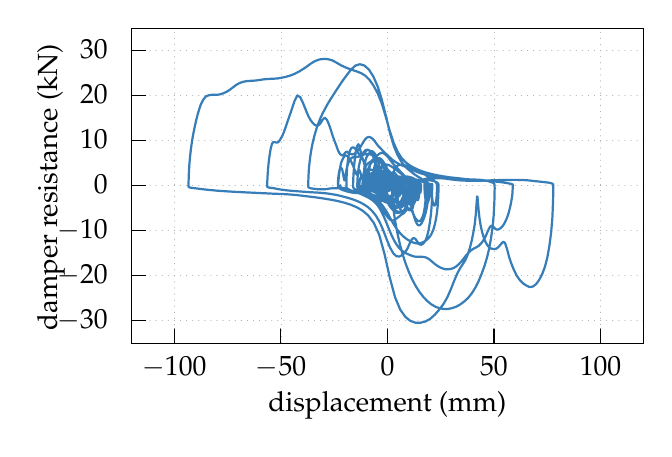
\begin{tikzpicture}[gnuplot]
%% generated with GNUPLOT 5.2p8 (Lua 5.3; terminal rev. Nov 2018, script rev. 108)
%% 08/29/2020 01:50:03
\path (0.000,0.000) rectangle (6.500,4.000);
\gpcolor{color=gp lt color axes}
\gpsetlinetype{gp lt axes}
\gpsetdashtype{gp dt axes}
\gpsetlinewidth{0.50}
\draw[gp path] (0.000,0.286)--(6.499,0.286);
\gpcolor{color=gp lt color border}
\gpsetlinetype{gp lt border}
\gpsetdashtype{gp dt solid}
\gpsetlinewidth{1.00}
\draw[gp path] (0.000,0.286)--(0.180,0.286);
\node[gp node right] at (-0.184,0.286) {$-30$};
\gpcolor{color=gp lt color axes}
\gpsetlinetype{gp lt axes}
\gpsetdashtype{gp dt axes}
\gpsetlinewidth{0.50}
\draw[gp path] (0.000,0.857)--(6.499,0.857);
\gpcolor{color=gp lt color border}
\gpsetlinetype{gp lt border}
\gpsetdashtype{gp dt solid}
\gpsetlinewidth{1.00}
\draw[gp path] (0.000,0.857)--(0.180,0.857);
\node[gp node right] at (-0.184,0.857) {$-20$};
\gpcolor{color=gp lt color axes}
\gpsetlinetype{gp lt axes}
\gpsetdashtype{gp dt axes}
\gpsetlinewidth{0.50}
\draw[gp path] (0.000,1.428)--(6.499,1.428);
\gpcolor{color=gp lt color border}
\gpsetlinetype{gp lt border}
\gpsetdashtype{gp dt solid}
\gpsetlinewidth{1.00}
\draw[gp path] (0.000,1.428)--(0.180,1.428);
\node[gp node right] at (-0.184,1.428) {$-10$};
\gpcolor{color=gp lt color axes}
\gpsetlinetype{gp lt axes}
\gpsetdashtype{gp dt axes}
\gpsetlinewidth{0.50}
\draw[gp path] (0.000,2.000)--(6.499,2.000);
\gpcolor{color=gp lt color border}
\gpsetlinetype{gp lt border}
\gpsetdashtype{gp dt solid}
\gpsetlinewidth{1.00}
\draw[gp path] (0.000,2.000)--(0.180,2.000);
\node[gp node right] at (-0.184,2.000) {$0$};
\gpcolor{color=gp lt color axes}
\gpsetlinetype{gp lt axes}
\gpsetdashtype{gp dt axes}
\gpsetlinewidth{0.50}
\draw[gp path] (0.000,2.571)--(6.499,2.571);
\gpcolor{color=gp lt color border}
\gpsetlinetype{gp lt border}
\gpsetdashtype{gp dt solid}
\gpsetlinewidth{1.00}
\draw[gp path] (0.000,2.571)--(0.180,2.571);
\node[gp node right] at (-0.184,2.571) {$10$};
\gpcolor{color=gp lt color axes}
\gpsetlinetype{gp lt axes}
\gpsetdashtype{gp dt axes}
\gpsetlinewidth{0.50}
\draw[gp path] (0.000,3.142)--(6.499,3.142);
\gpcolor{color=gp lt color border}
\gpsetlinetype{gp lt border}
\gpsetdashtype{gp dt solid}
\gpsetlinewidth{1.00}
\draw[gp path] (0.000,3.142)--(0.180,3.142);
\node[gp node right] at (-0.184,3.142) {$20$};
\gpcolor{color=gp lt color axes}
\gpsetlinetype{gp lt axes}
\gpsetdashtype{gp dt axes}
\gpsetlinewidth{0.50}
\draw[gp path] (0.000,3.713)--(6.499,3.713);
\gpcolor{color=gp lt color border}
\gpsetlinetype{gp lt border}
\gpsetdashtype{gp dt solid}
\gpsetlinewidth{1.00}
\draw[gp path] (0.000,3.713)--(0.180,3.713);
\node[gp node right] at (-0.184,3.713) {$30$};
\gpcolor{color=gp lt color axes}
\gpsetlinetype{gp lt axes}
\gpsetdashtype{gp dt axes}
\gpsetlinewidth{0.50}
\draw[gp path] (0.542,0.000)--(0.542,3.999);
\gpcolor{color=gp lt color border}
\gpsetlinetype{gp lt border}
\gpsetdashtype{gp dt solid}
\gpsetlinewidth{1.00}
\draw[gp path] (0.542,0.000)--(0.542,0.180);
\node[gp node center] at (0.542,-0.308) {$-100$};
\gpcolor{color=gp lt color axes}
\gpsetlinetype{gp lt axes}
\gpsetdashtype{gp dt axes}
\gpsetlinewidth{0.50}
\draw[gp path] (1.896,0.000)--(1.896,3.999);
\gpcolor{color=gp lt color border}
\gpsetlinetype{gp lt border}
\gpsetdashtype{gp dt solid}
\gpsetlinewidth{1.00}
\draw[gp path] (1.896,0.000)--(1.896,0.180);
\node[gp node center] at (1.896,-0.308) {$-50$};
\gpcolor{color=gp lt color axes}
\gpsetlinetype{gp lt axes}
\gpsetdashtype{gp dt axes}
\gpsetlinewidth{0.50}
\draw[gp path] (3.250,0.000)--(3.250,3.999);
\gpcolor{color=gp lt color border}
\gpsetlinetype{gp lt border}
\gpsetdashtype{gp dt solid}
\gpsetlinewidth{1.00}
\draw[gp path] (3.250,0.000)--(3.250,0.180);
\node[gp node center] at (3.250,-0.308) {$0$};
\gpcolor{color=gp lt color axes}
\gpsetlinetype{gp lt axes}
\gpsetdashtype{gp dt axes}
\gpsetlinewidth{0.50}
\draw[gp path] (4.603,0.000)--(4.603,3.999);
\gpcolor{color=gp lt color border}
\gpsetlinetype{gp lt border}
\gpsetdashtype{gp dt solid}
\gpsetlinewidth{1.00}
\draw[gp path] (4.603,0.000)--(4.603,0.180);
\node[gp node center] at (4.603,-0.308) {$50$};
\gpcolor{color=gp lt color axes}
\gpsetlinetype{gp lt axes}
\gpsetdashtype{gp dt axes}
\gpsetlinewidth{0.50}
\draw[gp path] (5.957,0.000)--(5.957,3.999);
\gpcolor{color=gp lt color border}
\gpsetlinetype{gp lt border}
\gpsetdashtype{gp dt solid}
\gpsetlinewidth{1.00}
\draw[gp path] (5.957,0.000)--(5.957,0.180);
\node[gp node center] at (5.957,-0.308) {$100$};
\draw[gp path] (0.000,3.999)--(0.000,0.000)--(6.499,0.000)--(6.499,3.999)--cycle;
\node[gp node center,rotate=-270] at (-1.028,1.999) {damper resistance (\si{\kilo\newton})};
\node[gp node center] at (3.249,-0.769) {displacement (\si{\milli\meter})};
\gpcolor{rgb color={0.216,0.494,0.722}}
\gpsetlinewidth{2.00}
\draw[gp path] (3.250,2.000)--(3.249,1.998)--(3.249,1.996)--(3.249,1.992)--(3.248,1.988)%
  --(3.248,1.985)--(3.247,1.982)--(3.246,1.980)--(3.244,1.977)--(3.243,1.974)--(3.241,1.971)%
  --(3.240,1.968)--(3.237,1.964)--(3.235,1.961)--(3.233,1.958)--(3.230,1.956)--(3.227,1.954)%
  --(3.224,1.953)--(3.221,1.952)--(3.218,1.952)--(3.215,1.951)--(3.212,1.951)--(3.208,1.950)%
  --(3.205,1.948)--(3.201,1.946)--(3.197,1.944)--(3.193,1.941)--(3.189,1.939)--(3.184,1.938)%
  --(3.179,1.937)--(3.174,1.937)--(3.169,1.937)--(3.164,1.938)--(3.159,1.939)--(3.154,1.940)%
  --(3.149,1.942)--(3.144,1.944)--(3.139,1.946)--(3.134,1.948)--(3.129,1.950)--(3.125,1.950)%
  --(3.120,1.950)--(3.115,1.950)--(3.110,1.949)--(3.105,1.948)--(3.099,1.949)--(3.094,1.950)%
  --(3.089,1.952)--(3.084,1.955)--(3.079,1.958)--(3.075,1.962)--(3.071,1.966)--(3.068,1.968)%
  --(3.065,1.969)--(3.061,1.969)--(3.058,1.969)--(3.055,1.969)--(3.052,1.969)--(3.048,1.968)%
  --(3.045,1.967)--(3.041,1.965)--(3.037,1.964)--(3.032,1.961)--(3.027,1.959)--(3.022,1.958)%
  --(3.017,1.956)--(3.011,1.956)--(3.005,1.956)--(2.999,1.956)--(2.993,1.957)--(2.987,1.957)%
  --(2.981,1.958)--(2.975,1.958)--(2.969,1.959)--(2.963,1.960)--(2.957,1.962)--(2.952,1.964)%
  --(2.947,1.967)--(2.942,1.970)--(2.939,1.974)--(2.936,1.979)--(2.934,1.984)--(2.933,1.991)%
  --(2.933,2.006)--(2.934,2.030)--(2.936,2.059)--(2.938,2.091)--(2.943,2.125)--(2.948,2.157)%
  --(2.954,2.187)--(2.961,2.212)--(2.969,2.234)--(2.978,2.252)--(2.988,2.267)--(2.998,2.278)%
  --(3.008,2.287)--(3.019,2.293)--(3.030,2.300)--(3.042,2.309)--(3.054,2.320)--(3.066,2.331)%
  --(3.079,2.344)--(3.093,2.358)--(3.108,2.372)--(3.124,2.386)--(3.140,2.399)--(3.158,2.410)%
  --(3.177,2.415)--(3.197,2.412)--(3.217,2.400)--(3.239,2.382)--(3.262,2.357)--(3.285,2.326)%
  --(3.308,2.295)--(3.332,2.267)--(3.357,2.240)--(3.381,2.214)--(3.405,2.190)--(3.428,2.165)%
  --(3.450,2.142)--(3.469,2.122)--(3.487,2.104)--(3.503,2.090)--(3.516,2.078)--(3.529,2.068)%
  --(3.539,2.059)--(3.549,2.053)--(3.558,2.048)--(3.565,2.044)--(3.572,2.041)--(3.579,2.040)%
  --(3.586,2.039)--(3.593,2.039)--(3.600,2.040)--(3.607,2.042)--(3.615,2.045)--(3.624,2.048)%
  --(3.634,2.052)--(3.646,2.057)--(3.659,2.063)--(3.674,2.068)--(3.692,2.074)--(3.712,2.080)%
  --(3.734,2.086)--(3.759,2.090)--(3.787,2.093)--(3.816,2.094)--(3.848,2.095)--(3.881,2.094)%
  --(3.915,2.093)--(3.950,2.092)--(3.986,2.090)--(4.023,2.089)--(4.061,2.088)--(4.100,2.086)%
  --(4.139,2.084)--(4.179,2.083)--(4.219,2.081)--(4.260,2.080)--(4.301,2.079)--(4.343,2.078)%
  --(4.386,2.076)--(4.428,2.074)--(4.469,2.069)--(4.507,2.063)--(4.540,2.054)--(4.567,2.046)%
  --(4.588,2.037)--(4.602,2.028)--(4.610,2.019)--(4.612,1.970)--(4.608,1.793)--(4.599,1.618)%
  --(4.584,1.462)--(4.564,1.322)--(4.541,1.195)--(4.513,1.080)--(4.481,0.975)--(4.446,0.878)%
  --(4.408,0.787)--(4.367,0.705)--(4.323,0.634)--(4.276,0.575)--(4.228,0.531)--(4.178,0.493)%
  --(4.127,0.464)--(4.074,0.445)--(4.021,0.434)--(3.968,0.433)--(3.914,0.442)--(3.861,0.462)%
  --(3.808,0.492)--(3.756,0.534)--(3.706,0.587)--(3.657,0.650)--(3.610,0.723)--(3.565,0.808)%
  --(3.523,0.901)--(3.484,1.003)--(3.448,1.113)--(3.415,1.229)--(3.387,1.350)--(3.362,1.470)%
  --(3.342,1.588)--(3.326,1.705)--(3.315,1.819)--(3.309,1.931)--(3.308,2.028)--(3.313,2.097)%
  --(3.323,2.158)--(3.340,2.206)--(3.362,2.240)--(3.390,2.260)--(3.424,2.266)--(3.464,2.260)%
  --(3.508,2.247)--(3.557,2.233)--(3.608,2.212)--(3.658,2.184)--(3.706,2.154)--(3.747,2.127)%
  --(3.783,2.103)--(3.812,2.084)--(3.836,2.068)--(3.854,2.052)--(3.867,2.038)--(3.875,2.026)%
  --(3.879,2.015)--(3.879,1.967)--(3.877,1.888)--(3.872,1.828)--(3.865,1.787)--(3.858,1.759)%
  --(3.849,1.746)--(3.841,1.749)--(3.833,1.766)--(3.825,1.795)--(3.819,1.835)--(3.814,1.884)%
  --(3.811,1.946)--(3.811,2.007)--(3.812,2.019)--(3.815,2.022)--(3.819,2.018)--(3.818,1.946)%
  --(3.814,1.779)--(3.804,1.646)--(3.790,1.540)--(3.773,1.437)--(3.753,1.352)--(3.730,1.296)%
  --(3.705,1.264)--(3.680,1.249)--(3.654,1.255)--(3.629,1.289)--(3.605,1.325)--(3.581,1.335)%
  --(3.557,1.314)--(3.531,1.261)--(3.503,1.198)--(3.472,1.152)--(3.439,1.120)--(3.403,1.100)%
  --(3.365,1.103)--(3.326,1.138)--(3.284,1.211)--(3.240,1.319)--(3.195,1.438)--(3.149,1.542)%
  --(3.101,1.623)--(3.052,1.682)--(3.003,1.727)--(2.953,1.761)--(2.902,1.788)--(2.852,1.810)%
  --(2.802,1.828)--(2.752,1.844)--(2.704,1.857)--(2.657,1.869)--(2.611,1.880)--(2.567,1.888)%
  --(2.524,1.895)--(2.482,1.901)--(2.440,1.905)--(2.399,1.909)--(2.357,1.912)--(2.316,1.914)%
  --(2.274,1.916)--(2.233,1.919)--(2.192,1.922)--(2.151,1.925)--(2.112,1.928)--(2.073,1.931)%
  --(2.036,1.934)--(2.000,1.937)--(1.966,1.941)--(1.935,1.945)--(1.905,1.949)--(1.879,1.953)%
  --(1.855,1.957)--(1.834,1.961)--(1.817,1.965)--(1.802,1.968)--(1.788,1.970)--(1.776,1.971)%
  --(1.765,1.972)--(1.755,1.974)--(1.746,1.976)--(1.738,1.977)--(1.732,1.979)--(1.727,1.982)%
  --(1.725,1.986)--(1.724,2.004)--(1.725,2.065)--(1.729,2.141)--(1.735,2.222)--(1.743,2.304)%
  --(1.754,2.387)--(1.768,2.470)--(1.784,2.533)--(1.802,2.554)--(1.819,2.552)--(1.837,2.548)%
  --(1.854,2.547)--(1.872,2.560)--(1.891,2.590)--(1.910,2.623)--(1.931,2.668)--(1.954,2.733)%
  --(1.979,2.808)--(2.006,2.884)--(2.036,2.971)--(2.070,3.075)--(2.106,3.145)--(2.143,3.123)%
  --(2.178,3.050)--(2.211,2.967)--(2.242,2.891)--(2.270,2.838)--(2.297,2.802)--(2.323,2.774)%
  --(2.348,2.761)--(2.373,2.766)--(2.399,2.791)--(2.426,2.835)--(2.454,2.863)--(2.481,2.837)%
  --(2.508,2.776)--(2.533,2.703)--(2.555,2.631)--(2.575,2.576)--(2.593,2.530)--(2.610,2.483)%
  --(2.625,2.441)--(2.640,2.414)--(2.653,2.397)--(2.666,2.387)--(2.679,2.385)--(2.693,2.394)%
  --(2.706,2.408)--(2.720,2.424)--(2.735,2.432)--(2.749,2.421)--(2.763,2.406)--(2.777,2.401)%
  --(2.790,2.400)--(2.804,2.398)--(2.818,2.399)--(2.832,2.406)--(2.846,2.416)--(2.860,2.428)%
  --(2.876,2.445)--(2.892,2.468)--(2.909,2.495)--(2.927,2.525)--(2.946,2.556)--(2.966,2.586)%
  --(2.988,2.610)--(3.011,2.618)--(3.034,2.613)--(3.057,2.599)--(3.080,2.576)--(3.102,2.546)%
  --(3.124,2.515)--(3.145,2.491)--(3.167,2.469)--(3.188,2.446)--(3.210,2.424)--(3.232,2.403)%
  --(3.256,2.382)--(3.280,2.359)--(3.306,2.335)--(3.334,2.313)--(3.364,2.293)--(3.397,2.274)%
  --(3.433,2.257)--(3.471,2.242)--(3.513,2.225)--(3.556,2.205)--(3.599,2.185)--(3.643,2.167)%
  --(3.686,2.152)--(3.728,2.141)--(3.770,2.131)--(3.812,2.122)--(3.853,2.115)--(3.893,2.107)%
  --(3.932,2.099)--(3.970,2.092)--(4.006,2.086)--(4.041,2.081)--(4.074,2.077)--(4.107,2.073)%
  --(4.138,2.070)--(4.169,2.067)--(4.200,2.065)--(4.230,2.064)--(4.260,2.062)--(4.290,2.062)%
  --(4.320,2.061)--(4.352,2.061)--(4.383,2.062)--(4.416,2.062)--(4.451,2.063)--(4.486,2.064)%
  --(4.524,2.066)--(4.564,2.067)--(4.605,2.068)--(4.649,2.070)--(4.695,2.071)--(4.743,2.072)%
  --(4.793,2.072)--(4.845,2.073)--(4.899,2.073)--(4.953,2.072)--(5.007,2.069)--(5.058,2.065)%
  --(5.105,2.059)--(5.148,2.055)--(5.187,2.050)--(5.222,2.047)--(5.254,2.043)--(5.282,2.040)%
  --(5.307,2.036)--(5.327,2.031)--(5.343,2.026)--(5.353,2.020)--(5.357,2.008)--(5.354,1.818)%
  --(5.345,1.594)--(5.329,1.403)--(5.307,1.235)--(5.281,1.088)--(5.250,0.968)--(5.215,0.875)%
  --(5.177,0.803)--(5.138,0.749)--(5.097,0.718)--(5.055,0.712)--(5.014,0.731)--(4.973,0.759)%
  --(4.933,0.798)--(4.895,0.853)--(4.859,0.923)--(4.826,1.004)--(4.795,1.096)--(4.768,1.198)%
  --(4.743,1.274)--(4.720,1.287)--(4.697,1.263)--(4.672,1.234)--(4.647,1.208)--(4.622,1.196)%
  --(4.596,1.196)--(4.570,1.200)--(4.544,1.214)--(4.520,1.242)--(4.496,1.284)--(4.474,1.339)%
  --(4.454,1.406)--(4.436,1.483)--(4.421,1.573)--(4.409,1.680)--(4.400,1.782)--(4.394,1.855)%
  --(4.389,1.863)--(4.382,1.770)--(4.372,1.631)--(4.359,1.510)--(4.341,1.402)--(4.320,1.299)%
  --(4.296,1.205)--(4.269,1.122)--(4.239,1.053)--(4.207,1.002)--(4.173,0.952)--(4.137,0.883)%
  --(4.099,0.795)--(4.057,0.687)--(4.010,0.580)--(3.961,0.495)--(3.908,0.425)--(3.852,0.361)%
  --(3.794,0.309)--(3.734,0.275)--(3.671,0.259)--(3.608,0.259)--(3.543,0.281)--(3.478,0.333)%
  --(3.412,0.426)--(3.346,0.585)--(3.280,0.832)--(3.213,1.132)--(3.146,1.375)--(3.077,1.527)%
  --(3.006,1.621)--(2.934,1.683)--(2.859,1.726)--(2.783,1.758)--(2.705,1.783)--(2.625,1.803)%
  --(2.544,1.819)--(2.463,1.833)--(2.382,1.845)--(2.301,1.856)--(2.221,1.865)--(2.143,1.875)%
  --(2.066,1.883)--(1.991,1.889)--(1.917,1.893)--(1.842,1.896)--(1.767,1.899)--(1.692,1.903)%
  --(1.618,1.906)--(1.544,1.910)--(1.472,1.913)--(1.401,1.917)--(1.332,1.920)--(1.266,1.924)%
  --(1.202,1.928)--(1.142,1.932)--(1.086,1.936)--(1.034,1.941)--(0.987,1.945)--(0.944,1.950)%
  --(0.906,1.954)--(0.873,1.958)--(0.844,1.962)--(0.819,1.965)--(0.796,1.968)--(0.777,1.970)%
  --(0.761,1.972)--(0.747,1.975)--(0.737,1.978)--(0.729,1.981)--(0.725,1.984)--(0.724,2.021)%
  --(0.727,2.129)--(0.733,2.246)--(0.743,2.363)--(0.756,2.479)--(0.773,2.594)--(0.794,2.706)%
  --(0.818,2.817)--(0.846,2.926)--(0.877,3.023)--(0.911,3.092)--(0.946,3.134)--(0.983,3.148)%
  --(1.020,3.154)--(1.057,3.154)--(1.094,3.154)--(1.132,3.161)--(1.169,3.174)--(1.208,3.192)%
  --(1.247,3.216)--(1.287,3.247)--(1.328,3.278)--(1.369,3.301)--(1.412,3.317)--(1.455,3.326)%
  --(1.498,3.330)--(1.542,3.332)--(1.585,3.336)--(1.629,3.342)--(1.673,3.349)--(1.717,3.353)%
  --(1.762,3.356)--(1.806,3.358)--(1.851,3.361)--(1.896,3.368)--(1.941,3.377)--(1.987,3.389)%
  --(2.033,3.404)--(2.080,3.424)--(2.128,3.449)--(2.177,3.479)--(2.227,3.513)--(2.278,3.550)%
  --(2.331,3.582)--(2.385,3.602)--(2.439,3.609)--(2.494,3.606)--(2.549,3.591)--(2.603,3.562)%
  --(2.657,3.530)--(2.710,3.505)--(2.762,3.484)--(2.814,3.466)--(2.866,3.448)--(2.919,3.427)%
  --(2.971,3.395)--(3.023,3.342)--(3.075,3.268)--(3.126,3.173)--(3.177,3.046)--(3.227,2.882)%
  --(3.278,2.701)--(3.329,2.544)--(3.380,2.429)--(3.431,2.350)--(3.483,2.295)--(3.536,2.256)%
  --(3.589,2.226)--(3.642,2.201)--(3.695,2.181)--(3.748,2.164)--(3.800,2.150)--(3.851,2.138)%
  --(3.902,2.128)--(3.951,2.119)--(4.000,2.112)--(4.047,2.105)--(4.094,2.100)--(4.140,2.095)%
  --(4.185,2.090)--(4.229,2.085)--(4.272,2.081)--(4.313,2.077)--(4.353,2.073)--(4.392,2.070)%
  --(4.429,2.066)--(4.465,2.064)--(4.500,2.061)--(4.534,2.058)--(4.567,2.056)--(4.598,2.053)%
  --(4.627,2.051)--(4.655,2.048)--(4.681,2.045)--(4.705,2.042)--(4.726,2.039)--(4.746,2.036)%
  --(4.763,2.033)--(4.778,2.031)--(4.792,2.028)--(4.803,2.026)--(4.813,2.024)--(4.821,2.022)%
  --(4.828,2.020)--(4.833,2.018)--(4.837,2.016)--(4.840,2.015)--(4.842,2.012)--(4.842,2.000)%
  --(4.841,1.966)--(4.839,1.925)--(4.836,1.886)--(4.832,1.851)--(4.826,1.819)--(4.820,1.783)%
  --(4.812,1.744)--(4.803,1.705)--(4.793,1.666)--(4.782,1.628)--(4.769,1.593)--(4.756,1.561)%
  --(4.741,1.531)--(4.726,1.504)--(4.710,1.482)--(4.693,1.465)--(4.676,1.452)--(4.658,1.443)%
  --(4.640,1.441)--(4.622,1.450)--(4.605,1.466)--(4.588,1.483)--(4.572,1.491)--(4.555,1.479)%
  --(4.538,1.450)--(4.519,1.408)--(4.500,1.361)--(4.478,1.321)--(4.456,1.287)--(4.432,1.258)%
  --(4.408,1.235)--(4.383,1.219)--(4.358,1.207)--(4.332,1.192)--(4.305,1.173)--(4.278,1.146)%
  --(4.249,1.114)--(4.220,1.076)--(4.189,1.037)--(4.156,1.002)--(4.123,0.973)--(4.089,0.953)%
  --(4.054,0.942)--(4.018,0.937)--(3.983,0.939)--(3.948,0.949)--(3.913,0.964)--(3.878,0.986)%
  --(3.844,1.011)--(3.811,1.040)--(3.779,1.066)--(3.748,1.084)--(3.716,1.094)--(3.685,1.096)%
  --(3.654,1.096)--(3.622,1.096)--(3.590,1.100)--(3.558,1.110)--(3.526,1.123)--(3.494,1.137)%
  --(3.462,1.154)--(3.429,1.178)--(3.397,1.210)--(3.365,1.253)--(3.333,1.307)--(3.301,1.373)%
  --(3.270,1.447)--(3.239,1.524)--(3.209,1.596)--(3.179,1.660)--(3.151,1.712)--(3.123,1.752)%
  --(3.095,1.784)--(3.068,1.808)--(3.042,1.827)--(3.016,1.843)--(2.991,1.856)--(2.966,1.868)%
  --(2.941,1.880)--(2.918,1.891)--(2.896,1.901)--(2.875,1.911)--(2.856,1.919)--(2.838,1.924)%
  --(2.821,1.929)--(2.804,1.933)--(2.789,1.937)--(2.773,1.939)--(2.758,1.942)--(2.744,1.944)%
  --(2.730,1.946)--(2.716,1.948)--(2.703,1.951)--(2.690,1.953)--(2.679,1.956)--(2.668,1.959)%
  --(2.658,1.962)--(2.649,1.965)--(2.641,1.969)--(2.635,1.973)--(2.631,1.978)--(2.628,1.983)%
  --(2.626,1.991)--(2.626,2.013)--(2.627,2.047)--(2.630,2.081)--(2.633,2.117)--(2.638,2.155)%
  --(2.644,2.197)--(2.652,2.242)--(2.660,2.283)--(2.670,2.311)--(2.681,2.333)--(2.693,2.356)%
  --(2.705,2.374)--(2.718,2.382)--(2.731,2.381)--(2.744,2.372)--(2.756,2.357)--(2.768,2.342)%
  --(2.779,2.325)--(2.790,2.305)--(2.800,2.283)--(2.810,2.262)--(2.818,2.242)--(2.826,2.221)%
  --(2.834,2.201)--(2.841,2.184)--(2.847,2.167)--(2.852,2.151)--(2.858,2.141)--(2.863,2.145)%
  --(2.868,2.158)--(2.874,2.178)--(2.881,2.195)--(2.888,2.200)--(2.895,2.194)--(2.902,2.179)%
  --(2.908,2.160)--(2.913,2.140)--(2.918,2.122)--(2.922,2.111)--(2.926,2.102)--(2.930,2.092)%
  --(2.933,2.082)--(2.937,2.076)--(2.939,2.072)--(2.942,2.067)--(2.945,2.063)--(2.947,2.061)%
  --(2.950,2.059)--(2.952,2.057)--(2.954,2.055)--(2.956,2.053)--(2.958,2.049)--(2.960,2.043)%
  --(2.962,2.036)--(2.964,2.031)--(2.965,2.027)--(2.966,2.026)--(2.967,2.028)--(2.969,2.034)%
  --(2.970,2.043)--(2.972,2.057)--(2.975,2.076)--(2.979,2.099)--(2.983,2.125)--(2.988,2.150)%
  --(2.994,2.174)--(3.001,2.198)--(3.009,2.221)--(3.017,2.241)--(3.027,2.260)--(3.037,2.277)%
  --(3.048,2.292)--(3.059,2.303)--(3.071,2.312)--(3.083,2.320)--(3.096,2.324)--(3.109,2.322)%
  --(3.122,2.317)--(3.136,2.314)--(3.149,2.310)--(3.163,2.302)--(3.176,2.296)--(3.190,2.293)%
  --(3.204,2.279)--(3.218,2.240)--(3.229,2.188)--(3.238,2.133)--(3.244,2.078)--(3.247,2.028)%
  --(3.247,1.980)--(3.245,1.934)--(3.240,1.894)--(3.232,1.861)--(3.222,1.836)--(3.210,1.819)%
  --(3.196,1.810)--(3.181,1.807)--(3.165,1.809)--(3.147,1.815)--(3.129,1.824)--(3.110,1.834)%
  --(3.091,1.844)--(3.071,1.855)--(3.052,1.866)--(3.033,1.876)--(3.015,1.886)--(2.997,1.895)%
  --(2.980,1.902)--(2.963,1.908)--(2.947,1.913)--(2.931,1.918)--(2.915,1.923)--(2.900,1.928)%
  --(2.886,1.934)--(2.873,1.940)--(2.862,1.945)--(2.851,1.950)--(2.841,1.954)--(2.832,1.959)%
  --(2.825,1.965)--(2.819,1.971)--(2.816,1.979)--(2.814,1.996)--(2.815,2.058)--(2.819,2.143)%
  --(2.826,2.237)--(2.836,2.339)--(2.849,2.434)--(2.865,2.503)--(2.883,2.526)--(2.900,2.480)%
  --(2.916,2.409)--(2.930,2.360)--(2.942,2.323)--(2.953,2.285)--(2.963,2.252)--(2.971,2.225)%
  --(2.979,2.191)--(2.985,2.137)--(2.989,2.079)--(2.992,2.033)--(2.992,2.001)--(2.992,1.986)%
  --(2.990,1.977)--(2.987,1.971)--(2.983,1.964)--(2.978,1.960)--(2.972,1.957)--(2.965,1.957)%
  --(2.959,1.960)--(2.954,1.965)--(2.950,1.973)--(2.947,1.987)--(2.948,2.043)--(2.951,2.141)%
  --(2.958,2.237)--(2.968,2.305)--(2.980,2.350)--(2.993,2.376)--(3.007,2.394)--(3.022,2.417)%
  --(3.038,2.436)--(3.055,2.438)--(3.072,2.427)--(3.088,2.409)--(3.104,2.383)--(3.119,2.348)%
  --(3.132,2.305)--(3.144,2.258)--(3.154,2.206)--(3.162,2.150)--(3.168,2.094)--(3.171,2.042)%
  --(3.172,1.999)--(3.171,1.976)--(3.169,1.962)--(3.166,1.954)--(3.162,1.953)--(3.158,1.955)%
  --(3.155,1.963)--(3.153,1.977)--(3.152,2.002)--(3.154,2.055)--(3.158,2.122)--(3.165,2.194)%
  --(3.175,2.244)--(3.186,2.246)--(3.197,2.227)--(3.209,2.215)--(3.220,2.205)--(3.230,2.193)%
  --(3.241,2.182)--(3.251,2.172)--(3.262,2.164)--(3.272,2.158)--(3.283,2.155)--(3.294,2.158)%
  --(3.306,2.163)--(3.319,2.168)--(3.334,2.167)--(3.348,2.155)--(3.363,2.137)--(3.376,2.118)%
  --(3.388,2.101)--(3.399,2.090)--(3.408,2.082)--(3.418,2.074)--(3.426,2.068)--(3.435,2.063)%
  --(3.442,2.060)--(3.450,2.057)--(3.457,2.056)--(3.465,2.057)--(3.473,2.060)--(3.482,2.063)%
  --(3.492,2.067)--(3.503,2.071)--(3.515,2.076)--(3.528,2.080)--(3.542,2.082)--(3.558,2.084)%
  --(3.574,2.083)--(3.590,2.082)--(3.607,2.079)--(3.624,2.075)--(3.640,2.071)--(3.655,2.067)%
  --(3.670,2.062)--(3.684,2.057)--(3.696,2.050)--(3.707,2.044)--(3.716,2.039)--(3.724,2.035)%
  --(3.731,2.033)--(3.737,2.031)--(3.744,2.030)--(3.750,2.031)--(3.757,2.032)--(3.763,2.031)%
  --(3.769,2.029)--(3.775,2.027)--(3.780,2.025)--(3.784,2.023)--(3.788,2.021)--(3.791,2.018)%
  --(3.793,2.014)--(3.794,2.006)--(3.793,1.983)--(3.792,1.946)--(3.789,1.906)--(3.785,1.871)%
  --(3.780,1.841)--(3.774,1.816)--(3.768,1.798)--(3.761,1.786)--(3.753,1.781)--(3.746,1.788)%
  --(3.739,1.805)--(3.733,1.832)--(3.727,1.868)--(3.724,1.912)--(3.721,1.962)--(3.721,2.006)%
  --(3.722,2.018)--(3.725,2.023)--(3.729,2.025)--(3.733,2.026)--(3.738,2.025)--(3.742,2.021)%
  --(3.744,2.016)--(3.745,2.008)--(3.745,1.990)--(3.744,1.962)--(3.742,1.923)--(3.738,1.864)%
  --(3.732,1.794)--(3.724,1.725)--(3.714,1.663)--(3.701,1.617)--(3.688,1.584)--(3.673,1.560)%
  --(3.658,1.548)--(3.642,1.550)--(3.627,1.561)--(3.612,1.577)--(3.597,1.600)--(3.584,1.629)%
  --(3.571,1.658)--(3.560,1.683)--(3.549,1.700)--(3.538,1.708)--(3.527,1.709)--(3.517,1.707)%
  --(3.506,1.700)--(3.495,1.691)--(3.483,1.678)--(3.471,1.664)--(3.458,1.650)--(3.444,1.641)%
  --(3.430,1.632)--(3.416,1.622)--(3.401,1.610)--(3.385,1.597)--(3.367,1.583)--(3.349,1.570)%
  --(3.330,1.560)--(3.309,1.557)--(3.287,1.564)--(3.264,1.586)--(3.240,1.617)--(3.216,1.653)%
  --(3.191,1.691)--(3.166,1.728)--(3.142,1.761)--(3.118,1.789)--(3.094,1.812)--(3.071,1.830)%
  --(3.048,1.845)--(3.026,1.859)--(3.003,1.869)--(2.982,1.878)--(2.960,1.885)--(2.938,1.890)%
  --(2.916,1.894)--(2.894,1.900)--(2.873,1.906)--(2.852,1.912)--(2.832,1.918)--(2.813,1.925)%
  --(2.796,1.933)--(2.780,1.940)--(2.767,1.947)--(2.755,1.955)--(2.745,1.961)--(2.737,1.966)%
  --(2.730,1.969)--(2.724,1.971)--(2.719,1.972)--(2.713,1.971)--(2.708,1.970)--(2.702,1.970)%
  --(2.695,1.969)--(2.689,1.969)--(2.683,1.970)--(2.676,1.971)--(2.671,1.972)--(2.666,1.974)%
  --(2.661,1.977)--(2.658,1.980)--(2.656,1.985)--(2.655,1.992)--(2.654,2.001)--(2.654,2.004)%
  --(2.655,2.000)--(2.654,1.994)--(2.654,1.988)--(2.652,1.983)--(2.649,1.979)--(2.646,1.976)%
  --(2.641,1.974)--(2.635,1.971)--(2.629,1.969)--(2.621,1.968)--(2.614,1.967)--(2.605,1.966)%
  --(2.597,1.966)--(2.588,1.966)--(2.579,1.966)--(2.571,1.967)--(2.562,1.967)--(2.554,1.967)%
  --(2.545,1.966)--(2.535,1.965)--(2.526,1.964)--(2.515,1.963)--(2.504,1.961)--(2.491,1.958)%
  --(2.478,1.956)--(2.463,1.955)--(2.447,1.954)--(2.431,1.953)--(2.414,1.953)--(2.397,1.954)%
  --(2.380,1.954)--(2.364,1.955)--(2.347,1.956)--(2.331,1.958)--(2.316,1.960)--(2.302,1.962)%
  --(2.289,1.964)--(2.277,1.966)--(2.266,1.970)--(2.257,1.973)--(2.251,1.977)--(2.246,1.981)%
  --(2.244,1.990)--(2.245,2.045)--(2.248,2.129)--(2.253,2.216)--(2.262,2.303)--(2.273,2.390)%
  --(2.287,2.475)--(2.304,2.557)--(2.324,2.637)--(2.346,2.714)--(2.370,2.785)--(2.397,2.853)%
  --(2.426,2.915)--(2.458,2.977)--(2.491,3.037)--(2.527,3.096)--(2.565,3.156)--(2.605,3.218)%
  --(2.648,3.283)--(2.693,3.348)--(2.741,3.413)--(2.792,3.478)--(2.845,3.525)--(2.901,3.542)%
  --(2.958,3.525)--(3.015,3.474)--(3.071,3.386)--(3.127,3.258)--(3.181,3.084)--(3.234,2.871)%
  --(3.284,2.662)--(3.332,2.500)--(3.379,2.388)--(3.423,2.310)--(3.466,2.255)--(3.506,2.213)%
  --(3.545,2.181)--(3.580,2.153)--(3.612,2.131)--(3.641,2.112)--(3.666,2.097)--(3.689,2.083)%
  --(3.709,2.071)--(3.726,2.061)--(3.740,2.052)--(3.751,2.043)--(3.760,2.036)--(3.767,2.028)%
  --(3.772,2.021)--(3.774,2.010)--(3.774,1.966)--(3.771,1.900)--(3.766,1.836)--(3.760,1.778)%
  --(3.751,1.725)--(3.741,1.676)--(3.729,1.633)--(3.716,1.593)--(3.702,1.558)--(3.686,1.526)%
  --(3.669,1.503)--(3.652,1.494)--(3.635,1.501)--(3.618,1.527)--(3.602,1.566)--(3.588,1.609)%
  --(3.575,1.655)--(3.563,1.697)--(3.553,1.739)--(3.545,1.787)--(3.538,1.832)--(3.532,1.867)%
  --(3.528,1.893)--(3.524,1.914)--(3.521,1.933)--(3.519,1.958)--(3.517,1.984)--(3.517,2.004)%
  --(3.518,2.015)--(3.520,2.020)--(3.522,2.024)--(3.526,2.027)--(3.529,2.028)--(3.533,2.028)%
  --(3.536,2.028)--(3.540,2.027)--(3.544,2.027)--(3.548,2.029)--(3.552,2.031)--(3.556,2.031)%
  --(3.561,2.032)--(3.565,2.031)--(3.570,2.031)--(3.575,2.032)--(3.580,2.032)--(3.585,2.032)%
  --(3.590,2.030)--(3.594,2.028)--(3.598,2.026)--(3.601,2.023)--(3.604,2.020)--(3.606,2.015)%
  --(3.607,2.008)--(3.608,1.995)--(3.607,1.977)--(3.606,1.959)--(3.604,1.943)--(3.601,1.931)%
  --(3.598,1.920)--(3.595,1.910)--(3.592,1.897)--(3.588,1.880)--(3.583,1.857)--(3.577,1.832)%
  --(3.571,1.806)--(3.563,1.784)--(3.555,1.767)--(3.547,1.759)--(3.538,1.757)--(3.529,1.763)%
  --(3.521,1.775)--(3.513,1.795)--(3.506,1.818)--(3.499,1.840)--(3.494,1.863)--(3.489,1.887)%
  --(3.485,1.910)--(3.482,1.932)--(3.480,1.951)--(3.478,1.970)--(3.477,1.984)--(3.476,1.989)%
  --(3.476,1.991)--(3.475,1.993)--(3.475,1.996)--(3.475,2.000)--(3.475,2.004)--(3.476,2.009)%
  --(3.477,2.014)--(3.478,2.019)--(3.481,2.024)--(3.484,2.029)--(3.488,2.034)--(3.492,2.038)%
  --(3.498,2.043)--(3.505,2.049)--(3.513,2.055)--(3.522,2.060)--(3.532,2.065)--(3.544,2.070)%
  --(3.557,2.073)--(3.571,2.073)--(3.585,2.071)--(3.599,2.067)--(3.612,2.063)--(3.625,2.058)%
  --(3.636,2.053)--(3.646,2.047)--(3.655,2.041)--(3.663,2.035)--(3.668,2.028)--(3.672,2.022)%
  --(3.675,2.016)--(3.676,2.006)--(3.676,1.985)--(3.675,1.954)--(3.672,1.928)--(3.670,1.913)%
  --(3.666,1.911)--(3.663,1.921)--(3.660,1.928)--(3.657,1.915)--(3.654,1.889)--(3.649,1.860)%
  --(3.644,1.834)--(3.638,1.820)--(3.631,1.816)--(3.625,1.820)--(3.619,1.832)--(3.613,1.854)%
  --(3.608,1.874)--(3.604,1.881)--(3.599,1.871)--(3.594,1.839)--(3.587,1.796)--(3.579,1.751)%
  --(3.570,1.714)--(3.559,1.696)--(3.548,1.689)--(3.537,1.686)--(3.526,1.688)--(3.515,1.697)%
  --(3.504,1.705)--(3.493,1.707)--(3.482,1.705)--(3.471,1.699)--(3.459,1.690)--(3.447,1.680)%
  --(3.435,1.670)--(3.422,1.664)--(3.409,1.659)--(3.395,1.655)--(3.381,1.653)--(3.366,1.655)%
  --(3.352,1.662)--(3.337,1.672)--(3.323,1.686)--(3.308,1.701)--(3.294,1.718)--(3.280,1.738)%
  --(3.266,1.760)--(3.253,1.784)--(3.241,1.808)--(3.230,1.831)--(3.219,1.856)--(3.211,1.886)%
  --(3.204,1.917)--(3.199,1.945)--(3.196,1.966)--(3.193,1.976)--(3.192,1.977)--(3.190,1.970)%
  --(3.187,1.955)--(3.183,1.934)--(3.177,1.912)--(3.169,1.895)--(3.159,1.882)--(3.148,1.873)%
  --(3.135,1.867)--(3.121,1.865)--(3.106,1.866)--(3.091,1.869)--(3.075,1.874)--(3.058,1.881)%
  --(3.042,1.888)--(3.026,1.895)--(3.010,1.902)--(2.995,1.909)--(2.981,1.917)--(2.967,1.926)%
  --(2.955,1.934)--(2.944,1.938)--(2.933,1.940)--(2.922,1.940)--(2.911,1.939)--(2.899,1.938)%
  --(2.887,1.938)--(2.874,1.936)--(2.860,1.934)--(2.846,1.933)--(2.831,1.933)--(2.816,1.934)%
  --(2.800,1.936)--(2.785,1.939)--(2.771,1.944)--(2.758,1.950)--(2.747,1.957)--(2.738,1.965)%
  --(2.732,1.973)--(2.729,1.985)--(2.729,2.043)--(2.733,2.144)--(2.739,2.242)--(2.749,2.326)%
  --(2.761,2.395)--(2.775,2.445)--(2.791,2.475)--(2.807,2.486)--(2.824,2.483)--(2.840,2.469)%
  --(2.856,2.447)--(2.871,2.423)--(2.886,2.403)--(2.900,2.393)--(2.914,2.390)--(2.927,2.390)%
  --(2.941,2.396)--(2.956,2.414)--(2.971,2.433)--(2.987,2.448)--(3.004,2.453)--(3.020,2.448)%
  --(3.037,2.436)--(3.053,2.420)--(3.069,2.401)--(3.084,2.380)--(3.099,2.360)--(3.113,2.345)%
  --(3.127,2.332)--(3.141,2.320)--(3.155,2.307)--(3.168,2.291)--(3.181,2.272)--(3.194,2.252)%
  --(3.206,2.231)--(3.217,2.210)--(3.228,2.187)--(3.237,2.162)--(3.246,2.136)--(3.253,2.108)%
  --(3.259,2.083)--(3.263,2.061)--(3.267,2.045)--(3.269,2.035)--(3.271,2.029)--(3.273,2.024)%
  --(3.275,2.022)--(3.276,2.024)--(3.278,2.028)--(3.280,2.032)--(3.282,2.037)--(3.285,2.043)%
  --(3.288,2.049)--(3.291,2.056)--(3.296,2.064)--(3.301,2.074)--(3.306,2.083)--(3.313,2.085)%
  --(3.319,2.082)--(3.325,2.070)--(3.331,2.056)--(3.335,2.042)--(3.338,2.030)--(3.340,2.023)%
  --(3.341,2.018)--(3.343,2.016)--(3.344,2.016)--(3.345,2.021)--(3.347,2.028)--(3.350,2.036)%
  --(3.353,2.044)--(3.357,2.048)--(3.362,2.049)--(3.366,2.048)--(3.371,2.045)--(3.374,2.040)%
  --(3.378,2.035)--(3.381,2.032)--(3.384,2.031)--(3.387,2.033)--(3.390,2.037)--(3.394,2.042)%
  --(3.399,2.050)--(3.405,2.059)--(3.412,2.068)--(3.421,2.074)--(3.430,2.078)--(3.440,2.079)%
  --(3.451,2.077)--(3.461,2.073)--(3.471,2.068)--(3.480,2.062)--(3.489,2.055)--(3.496,2.049)%
  --(3.503,2.043)--(3.508,2.037)--(3.513,2.032)--(3.517,2.028)--(3.520,2.024)--(3.523,2.022)%
  --(3.525,2.020)--(3.527,2.020)--(3.530,2.020)--(3.532,2.017)--(3.533,2.013)--(3.534,2.005)%
  --(3.534,1.988)--(3.532,1.957)--(3.530,1.922)--(3.526,1.891)--(3.522,1.867)--(3.517,1.849)%
  --(3.511,1.838)--(3.505,1.833)--(3.499,1.834)--(3.493,1.841)--(3.487,1.848)--(3.481,1.848)%
  --(3.475,1.845)--(3.469,1.845)--(3.463,1.849)--(3.458,1.860)--(3.453,1.875)--(3.448,1.894)%
  --(3.444,1.918)--(3.442,1.946)--(3.440,1.974)--(3.439,1.996)--(3.439,2.009)--(3.440,2.016)%
  --(3.442,2.021)--(3.444,2.025)--(3.447,2.028)--(3.451,2.033)--(3.455,2.038)--(3.460,2.044)%
  --(3.466,2.050)--(3.473,2.055)--(3.481,2.059)--(3.489,2.059)--(3.498,2.056)--(3.506,2.051)%
  --(3.513,2.045)--(3.519,2.037)--(3.524,2.028)--(3.526,2.017)--(3.527,2.000)--(3.526,1.969)%
  --(3.525,1.939)--(3.522,1.914)--(3.518,1.896)--(3.514,1.885)--(3.510,1.880)--(3.505,1.880)%
  --(3.500,1.879)--(3.496,1.872)--(3.491,1.858)--(3.485,1.839)--(3.478,1.815)--(3.471,1.789)%
  --(3.462,1.764)--(3.453,1.746)--(3.443,1.734)--(3.433,1.727)--(3.422,1.725)--(3.411,1.729)%
  --(3.401,1.738)--(3.391,1.752)--(3.381,1.766)--(3.371,1.778)--(3.362,1.787)--(3.353,1.792)%
  --(3.344,1.795)--(3.335,1.797)--(3.326,1.797)--(3.316,1.793)--(3.306,1.788)--(3.296,1.784)%
  --(3.285,1.783)--(3.273,1.790)--(3.262,1.800)--(3.251,1.814)--(3.240,1.830)--(3.230,1.848)%
  --(3.221,1.868)--(3.212,1.888)--(3.205,1.908)--(3.199,1.928)--(3.195,1.947)--(3.192,1.964)%
  --(3.190,1.979)--(3.189,1.991)--(3.188,1.999)--(3.188,2.000)--(3.188,1.991)--(3.187,1.973)%
  --(3.184,1.954)--(3.180,1.938)--(3.175,1.926)--(3.168,1.917)--(3.161,1.912)--(3.153,1.910)%
  --(3.145,1.911)--(3.137,1.915)--(3.129,1.921)--(3.121,1.930)--(3.115,1.939)--(3.109,1.947)%
  --(3.104,1.954)--(3.099,1.959)--(3.096,1.963)--(3.092,1.970)--(3.090,1.977)--(3.088,1.985)%
  --(3.088,1.994)--(3.088,2.005)--(3.088,2.018)--(3.089,2.030)--(3.091,2.042)--(3.093,2.053)%
  --(3.096,2.063)--(3.098,2.072)--(3.102,2.078)--(3.105,2.080)--(3.108,2.077)--(3.112,2.070)%
  --(3.114,2.059)--(3.117,2.043)--(3.118,2.026)--(3.119,2.011)--(3.119,2.000)--(3.119,1.995)%
  --(3.119,1.993)--(3.118,1.996)--(3.118,2.002)--(3.119,2.009)--(3.119,2.011)--(3.120,2.008)%
  --(3.120,2.002)--(3.120,1.995)--(3.119,1.990)--(3.118,1.984)--(3.117,1.978)--(3.115,1.973)%
  --(3.113,1.970)--(3.110,1.968)--(3.107,1.966)--(3.104,1.965)--(3.100,1.965)--(3.097,1.964)%
  --(3.093,1.964)--(3.090,1.964)--(3.086,1.965)--(3.083,1.968)--(3.080,1.970)--(3.077,1.971)%
  --(3.074,1.972)--(3.071,1.971)--(3.069,1.972)--(3.066,1.973)--(3.063,1.976)--(3.062,1.981)%
  --(3.061,1.990)--(3.060,2.010)--(3.062,2.047)--(3.065,2.094)--(3.070,2.144)--(3.076,2.194)%
  --(3.085,2.239)--(3.095,2.277)--(3.107,2.309)--(3.120,2.332)--(3.134,2.346)--(3.149,2.349)%
  --(3.164,2.342)--(3.180,2.327)--(3.195,2.307)--(3.210,2.284)--(3.224,2.258)--(3.237,2.232)%
  --(3.250,2.209)--(3.263,2.188)--(3.274,2.171)--(3.286,2.157)--(3.296,2.146)--(3.307,2.137)%
  --(3.318,2.129)--(3.328,2.124)--(3.339,2.120)--(3.350,2.115)--(3.361,2.109)--(3.371,2.101)%
  --(3.381,2.093)--(3.391,2.084)--(3.400,2.075)--(3.408,2.064)--(3.414,2.053)--(3.420,2.041)%
  --(3.423,2.029)--(3.425,2.015)--(3.426,1.995)--(3.425,1.966)--(3.423,1.937)--(3.420,1.912)%
  --(3.416,1.894)--(3.411,1.882)--(3.407,1.875)--(3.401,1.873)--(3.396,1.875)--(3.391,1.878)%
  --(3.386,1.876)--(3.381,1.871)--(3.375,1.863)--(3.369,1.852)--(3.363,1.838)--(3.355,1.825)%
  --(3.348,1.815)--(3.339,1.808)--(3.330,1.802)--(3.321,1.799)--(3.312,1.797)--(3.302,1.795)%
  --(3.291,1.791)--(3.281,1.788)--(3.269,1.785)--(3.257,1.783)--(3.244,1.784)--(3.231,1.788)%
  --(3.217,1.794)--(3.202,1.801)--(3.187,1.810)--(3.172,1.820)--(3.156,1.830)--(3.140,1.840)%
  --(3.124,1.849)--(3.108,1.858)--(3.092,1.867)--(3.076,1.876)--(3.060,1.884)--(3.044,1.894)%
  --(3.030,1.906)--(3.017,1.919)--(3.005,1.931)--(2.996,1.944)--(2.989,1.957)--(2.984,1.970)%
  --(2.981,1.982)--(2.981,2.005)--(2.982,2.053)--(2.985,2.100)--(2.989,2.134)--(2.995,2.156)%
  --(3.001,2.165)--(3.007,2.166)--(3.013,2.164)--(3.019,2.158)--(3.025,2.148)--(3.031,2.137)%
  --(3.036,2.129)--(3.041,2.124)--(3.045,2.119)--(3.050,2.116)--(3.055,2.115)--(3.059,2.114)%
  --(3.064,2.114)--(3.068,2.114)--(3.073,2.117)--(3.078,2.121)--(3.083,2.125)--(3.088,2.128)%
  --(3.093,2.129)--(3.099,2.125)--(3.104,2.119)--(3.108,2.112)--(3.113,2.104)--(3.117,2.099)%
  --(3.122,2.099)--(3.126,2.101)--(3.130,2.104)--(3.135,2.108)--(3.140,2.113)--(3.145,2.116)%
  --(3.150,2.116)--(3.155,2.112)--(3.160,2.105)--(3.164,2.096)--(3.169,2.086)--(3.173,2.079)%
  --(3.176,2.077)--(3.180,2.079)--(3.184,2.084)--(3.188,2.091)--(3.193,2.096)--(3.198,2.097)%
  --(3.202,2.094)--(3.207,2.086)--(3.211,2.075)--(3.215,2.063)--(3.218,2.051)--(3.220,2.042)%
  --(3.223,2.037)--(3.225,2.035)--(3.227,2.034)--(3.228,2.034)--(3.230,2.036)--(3.233,2.037)%
  --(3.235,2.040)--(3.237,2.042)--(3.240,2.045)--(3.242,2.048)--(3.245,2.051)--(3.248,2.053)%
  --(3.251,2.057)--(3.255,2.061)--(3.259,2.064)--(3.263,2.069)--(3.267,2.073)--(3.272,2.077)%
  --(3.278,2.082)--(3.283,2.086)--(3.289,2.090)--(3.296,2.094)--(3.303,2.098)--(3.311,2.101)%
  --(3.319,2.104)--(3.328,2.107)--(3.337,2.109)--(3.347,2.111)--(3.358,2.113)--(3.369,2.114)%
  --(3.381,2.114)--(3.394,2.112)--(3.407,2.109)--(3.420,2.104)--(3.433,2.099)--(3.446,2.093)%
  --(3.459,2.087)--(3.471,2.080)--(3.482,2.074)--(3.493,2.068)--(3.503,2.064)--(3.513,2.061)%
  --(3.522,2.057)--(3.531,2.053)--(3.540,2.048)--(3.547,2.042)--(3.553,2.034)--(3.557,2.025)%
  --(3.559,2.016)--(3.560,1.997)--(3.559,1.957)--(3.556,1.915)--(3.553,1.880)--(3.548,1.855)%
  --(3.542,1.843)--(3.537,1.842)--(3.531,1.853)--(3.526,1.869)--(3.521,1.884)--(3.517,1.896)%
  --(3.513,1.898)--(3.509,1.896)--(3.505,1.892)--(3.501,1.888)--(3.496,1.882)--(3.492,1.875)%
  --(3.487,1.865)--(3.481,1.851)--(3.475,1.832)--(3.469,1.809)--(3.461,1.785)--(3.452,1.765)%
  --(3.443,1.754)--(3.434,1.751)--(3.424,1.756)--(3.415,1.765)--(3.406,1.775)--(3.397,1.787)%
  --(3.388,1.799)--(3.380,1.811)--(3.373,1.824)--(3.366,1.837)--(3.359,1.852)--(3.353,1.868)%
  --(3.347,1.884)--(3.343,1.902)--(3.339,1.919)--(3.335,1.934)--(3.332,1.943)--(3.330,1.946)%
  --(3.327,1.941)--(3.324,1.930)--(3.320,1.916)--(3.316,1.901)--(3.311,1.887)--(3.305,1.876)%
  --(3.299,1.865)--(3.292,1.856)--(3.284,1.848)--(3.276,1.841)--(3.267,1.835)--(3.258,1.831)%
  --(3.248,1.831)--(3.238,1.833)--(3.227,1.839)--(3.217,1.848)--(3.206,1.860)--(3.197,1.873)%
  --(3.188,1.889)--(3.179,1.904)--(3.172,1.918)--(3.166,1.930)--(3.160,1.940)--(3.156,1.947)%
  --(3.151,1.953)--(3.148,1.957)--(3.144,1.958)--(3.140,1.958)--(3.137,1.957)--(3.133,1.955)%
  --(3.129,1.951)--(3.124,1.947)--(3.118,1.944)--(3.113,1.941)--(3.107,1.941)--(3.100,1.942)%
  --(3.094,1.945)--(3.089,1.950)--(3.084,1.957)--(3.080,1.965)--(3.077,1.975)--(3.075,1.986)%
  --(3.075,2.001)--(3.075,2.019)--(3.076,2.033)--(3.078,2.040)--(3.080,2.043)--(3.082,2.041)%
  --(3.083,2.036)--(3.085,2.028)--(3.086,2.017)--(3.086,2.006)--(3.086,1.995)--(3.086,1.987)%
  --(3.085,1.981)--(3.083,1.976)--(3.080,1.970)--(3.077,1.965)--(3.073,1.961)--(3.069,1.956)%
  --(3.063,1.952)--(3.057,1.947)--(3.050,1.943)--(3.043,1.940)--(3.035,1.938)--(3.026,1.936)%
  --(3.017,1.935)--(3.008,1.934)--(2.998,1.934)--(2.987,1.935)--(2.977,1.936)--(2.967,1.938)%
  --(2.957,1.941)--(2.947,1.945)--(2.938,1.948)--(2.930,1.952)--(2.922,1.955)--(2.914,1.958)%
  --(2.908,1.960)--(2.901,1.962)--(2.895,1.964)--(2.889,1.965)--(2.884,1.967)--(2.879,1.969)%
  --(2.874,1.972)--(2.871,1.977)--(2.868,1.982)--(2.867,1.993)--(2.868,2.030)--(2.870,2.083)%
  --(2.874,2.138)--(2.880,2.191)--(2.887,2.242)--(2.897,2.290)--(2.908,2.333)--(2.920,2.371)%
  --(2.934,2.402)--(2.949,2.427)--(2.964,2.444)--(2.981,2.454)--(2.997,2.456)--(3.014,2.450)%
  --(3.030,2.436)--(3.046,2.413)--(3.062,2.385)--(3.076,2.353)--(3.089,2.321)--(3.101,2.287)%
  --(3.112,2.253)--(3.122,2.220)--(3.131,2.191)--(3.138,2.165)--(3.145,2.141)--(3.151,2.121)%
  --(3.156,2.104)--(3.160,2.094)--(3.165,2.089)--(3.169,2.091)--(3.173,2.099)--(3.178,2.112)%
  --(3.184,2.129)--(3.191,2.148)--(3.199,2.168)--(3.207,2.186)--(3.217,2.198)--(3.228,2.204)%
  --(3.240,2.205)--(3.252,2.201)--(3.264,2.193)--(3.276,2.182)--(3.288,2.169)--(3.300,2.155)%
  --(3.311,2.139)--(3.322,2.122)--(3.332,2.106)--(3.340,2.092)--(3.348,2.082)--(3.355,2.076)%
  --(3.362,2.071)--(3.369,2.069)--(3.376,2.070)--(3.384,2.072)--(3.392,2.076)--(3.400,2.081)%
  --(3.410,2.087)--(3.421,2.091)--(3.433,2.095)--(3.446,2.096)--(3.459,2.096)--(3.474,2.095)%
  --(3.488,2.092)--(3.503,2.088)--(3.517,2.083)--(3.530,2.077)--(3.543,2.070)--(3.555,2.063)%
  --(3.566,2.055)--(3.575,2.046)--(3.582,2.038)--(3.587,2.028)--(3.590,2.017)--(3.590,1.991)%
  --(3.589,1.933)--(3.585,1.876)--(3.580,1.830)--(3.573,1.794)--(3.566,1.769)--(3.557,1.756)%
  --(3.549,1.759)--(3.540,1.773)--(3.532,1.793)--(3.525,1.821)--(3.519,1.856)--(3.515,1.894)%
  --(3.511,1.931)--(3.509,1.962)--(3.508,1.983)--(3.507,1.997)--(3.507,2.006)--(3.508,2.011)%
  --(3.509,2.015)--(3.511,2.017)--(3.513,2.019)--(3.515,2.020)--(3.517,2.019)--(3.518,2.016)%
  --(3.520,2.011)--(3.520,2.002)--(3.520,1.988)--(3.519,1.974)--(3.518,1.963)--(3.516,1.955)%
  --(3.514,1.952)--(3.512,1.952)--(3.510,1.958)--(3.509,1.968)--(3.508,1.980)--(3.507,1.994)%
  --(3.507,2.007)--(3.508,2.014)--(3.510,2.020)--(3.512,2.023)--(3.515,2.025)--(3.518,2.026)%
  --(3.521,2.026)--(3.525,2.025)--(3.527,2.022)--(3.530,2.019)--(3.531,2.014)--(3.532,2.005)%
  --(3.532,1.988)--(3.531,1.963)--(3.529,1.933)--(3.526,1.901)--(3.521,1.868)--(3.516,1.835)%
  --(3.509,1.802)--(3.501,1.770)--(3.492,1.742)--(3.482,1.718)--(3.471,1.699)--(3.460,1.685)%
  --(3.448,1.674)--(3.435,1.668)--(3.422,1.665)--(3.409,1.665)--(3.396,1.667)--(3.382,1.670)%
  --(3.368,1.675)--(3.355,1.682)--(3.341,1.690)--(3.327,1.701)--(3.314,1.714)--(3.300,1.729)%
  --(3.287,1.744)--(3.274,1.761)--(3.261,1.779)--(3.249,1.795)--(3.237,1.809)--(3.225,1.821)%
  --(3.213,1.831)--(3.201,1.839)--(3.189,1.846)--(3.176,1.851)--(3.164,1.855)--(3.151,1.859)%
  --(3.137,1.862)--(3.123,1.865)--(3.109,1.869)--(3.094,1.874)--(3.078,1.878)--(3.063,1.883)%
  --(3.047,1.887)--(3.030,1.890)--(3.014,1.893)--(2.997,1.896)--(2.979,1.898)--(2.961,1.899)%
  --(2.942,1.901)--(2.923,1.902)--(2.902,1.903)--(2.881,1.904)--(2.860,1.906)--(2.838,1.908)%
  --(2.815,1.910)--(2.792,1.913)--(2.770,1.918)--(2.748,1.923)--(2.728,1.929)--(2.709,1.935)%
  --(2.691,1.940)--(2.675,1.947)--(2.661,1.953)--(2.650,1.959)--(2.640,1.965)--(2.633,1.971)%
  --(2.627,1.976)--(2.623,1.981)--(2.622,1.988)--(2.621,2.008)--(2.622,2.047)--(2.625,2.089)%
  --(2.629,2.126)--(2.634,2.161)--(2.640,2.193)--(2.647,2.217)--(2.654,2.228)--(2.662,2.227)%
  --(2.669,2.217)--(2.677,2.198)--(2.683,2.173)--(2.688,2.144)--(2.693,2.116)--(2.697,2.092)%
  --(2.700,2.077)--(2.703,2.069)--(2.705,2.067)--(2.708,2.073)--(2.711,2.087)--(2.714,2.108)%
  --(2.719,2.135)--(2.724,2.167)--(2.730,2.203)--(2.738,2.238)--(2.747,2.268)--(2.756,2.294)%
  --(2.767,2.316)--(2.778,2.333)--(2.789,2.347)--(2.801,2.356)--(2.814,2.361)--(2.826,2.363)%
  --(2.839,2.364)--(2.851,2.363)--(2.864,2.365)--(2.877,2.367)--(2.890,2.370)--(2.903,2.374)%
  --(2.916,2.379)--(2.930,2.384)--(2.943,2.391)--(2.957,2.396)--(2.972,2.400)--(2.986,2.402)%
  --(3.001,2.402)--(3.016,2.400)--(3.031,2.397)--(3.046,2.392)--(3.061,2.384)--(3.075,2.376)%
  --(3.090,2.367)--(3.104,2.357)--(3.119,2.348)--(3.133,2.338)--(3.147,2.327)--(3.162,2.313)%
  --(3.175,2.297)--(3.189,2.278)--(3.202,2.257)--(3.215,2.234)--(3.226,2.209)--(3.237,2.184)%
  --(3.247,2.159)--(3.256,2.133)--(3.263,2.107)--(3.270,2.086)--(3.275,2.071)--(3.279,2.063)%
  --(3.283,2.060)--(3.287,2.060)--(3.292,2.062)--(3.296,2.066)--(3.301,2.073)--(3.307,2.082)%
  --(3.314,2.092)--(3.322,2.101)--(3.331,2.109)--(3.340,2.114)--(3.351,2.117)--(3.363,2.118)%
  --(3.375,2.117)--(3.387,2.116)--(3.401,2.115)--(3.414,2.112)--(3.429,2.110)--(3.443,2.107)%
  --(3.458,2.104)--(3.473,2.100)--(3.488,2.096)--(3.504,2.092)--(3.519,2.087)--(3.533,2.081)%
  --(3.547,2.075)--(3.560,2.068)--(3.572,2.061)--(3.583,2.055)--(3.593,2.049)--(3.601,2.043)%
  --(3.609,2.038)--(3.615,2.033)--(3.620,2.028)--(3.624,2.024)--(3.627,2.019)--(3.629,2.014)%
  --(3.630,2.005)--(3.629,1.987)--(3.628,1.960)--(3.626,1.931)--(3.623,1.900)--(3.619,1.871)%
  --(3.614,1.844)--(3.608,1.819)--(3.601,1.798)--(3.593,1.781)--(3.585,1.768)--(3.577,1.762)%
  --(3.569,1.763)--(3.560,1.769)--(3.552,1.781)--(3.545,1.794)--(3.537,1.805)--(3.530,1.815)%
  --(3.524,1.823)--(3.517,1.831)--(3.511,1.838)--(3.505,1.844)--(3.499,1.849)--(3.494,1.854)%
  --(3.488,1.857)--(3.483,1.861)--(3.478,1.863)--(3.473,1.866)--(3.467,1.868)--(3.462,1.869)%
  --(3.457,1.868)--(3.452,1.863)--(3.447,1.855)--(3.441,1.844)--(3.434,1.830)--(3.427,1.813)%
  --(3.420,1.792)--(3.411,1.770)--(3.401,1.750)--(3.391,1.734)--(3.380,1.723)--(3.368,1.717)%
  --(3.356,1.716)--(3.344,1.719)--(3.332,1.726)--(3.319,1.738)--(3.307,1.752)--(3.295,1.769)%
  --(3.284,1.787)--(3.273,1.804)--(3.263,1.820)--(3.253,1.835)--(3.244,1.849)--(3.235,1.861)%
  --(3.226,1.871)--(3.218,1.879)--(3.210,1.884)--(3.201,1.887)--(3.193,1.887)--(3.184,1.888)%
  --(3.175,1.888)--(3.166,1.890)--(3.156,1.896)--(3.147,1.904)--(3.139,1.913)--(3.131,1.922)%
  --(3.123,1.931)--(3.117,1.938)--(3.111,1.943)--(3.105,1.946)--(3.099,1.948)--(3.094,1.949)%
  --(3.088,1.948)--(3.083,1.947)--(3.077,1.947)--(3.071,1.949)--(3.065,1.951)--(3.059,1.954)%
  --(3.054,1.958)--(3.049,1.962)--(3.046,1.968)--(3.043,1.974)--(3.041,1.983)--(3.040,1.995)%
  --(3.040,2.016)--(3.041,2.039)--(3.043,2.054)--(3.046,2.062)--(3.048,2.062)--(3.050,2.054)%
  --(3.052,2.037)--(3.054,2.016)--(3.054,1.999)--(3.054,1.989)--(3.053,1.984)--(3.051,1.981)%
  --(3.049,1.980)--(3.048,1.981)--(3.046,1.985)--(3.045,1.992)--(3.045,2.003)--(3.046,2.018)%
  --(3.047,2.030)--(3.049,2.039)--(3.050,2.045)--(3.052,2.047)--(3.054,2.044)--(3.056,2.036)%
  --(3.057,2.023)--(3.058,2.006)--(3.058,1.992)--(3.057,1.981)--(3.055,1.972)--(3.051,1.963)%
  --(3.046,1.956)--(3.041,1.952)--(3.034,1.950)--(3.028,1.951)--(3.022,1.954)--(3.016,1.959)%
  --(3.011,1.966)--(3.008,1.975)--(3.006,1.990)--(3.007,2.032)--(3.009,2.098)--(3.014,2.167)%
  --(3.022,2.226)--(3.031,2.274)--(3.042,2.304)--(3.054,2.320)--(3.066,2.323)--(3.079,2.314)%
  --(3.091,2.292)--(3.102,2.257)--(3.111,2.212)--(3.119,2.158)--(3.124,2.098)--(3.127,2.040)%
  --(3.128,1.999)--(3.127,1.979)--(3.125,1.968)--(3.122,1.960)--(3.118,1.957)--(3.114,1.958)%
  --(3.110,1.962)--(3.107,1.970)--(3.105,1.980)--(3.104,1.994)--(3.104,2.013)--(3.105,2.034)%
  --(3.107,2.053)--(3.110,2.069)--(3.113,2.080)--(3.117,2.089)--(3.121,2.101)--(3.126,2.115)%
  --(3.131,2.132)--(3.137,2.150)--(3.144,2.170)--(3.152,2.192)--(3.161,2.213)--(3.171,2.232)%
  --(3.182,2.245)--(3.194,2.255)--(3.207,2.262)--(3.221,2.267)--(3.236,2.268)--(3.251,2.266)%
  --(3.268,2.261)--(3.285,2.252)--(3.304,2.241)--(3.323,2.229)--(3.343,2.214)--(3.363,2.199)%
  --(3.384,2.182)--(3.405,2.165)--(3.425,2.150)--(3.444,2.135)--(3.463,2.121)--(3.481,2.109)%
  --(3.497,2.098)--(3.513,2.088)--(3.527,2.078)--(3.540,2.070)--(3.551,2.062)--(3.562,2.054)%
  --(3.570,2.046)--(3.578,2.038)--(3.583,2.030)--(3.587,2.021)--(3.588,2.008)--(3.588,1.969)%
  --(3.586,1.913)--(3.581,1.857)--(3.575,1.803)--(3.567,1.755)--(3.558,1.720)--(3.547,1.697)%
  --(3.537,1.688)--(3.525,1.690)--(3.514,1.703)--(3.504,1.726)--(3.494,1.755)--(3.486,1.790)%
  --(3.479,1.825)--(3.473,1.860)--(3.468,1.889)--(3.464,1.914)--(3.461,1.933)--(3.458,1.947)%
  --(3.456,1.958)--(3.455,1.969)--(3.454,1.984)--(3.453,2.000)--(3.454,2.013)--(3.456,2.022)%
  --(3.458,2.030)--(3.462,2.036)--(3.467,2.039)--(3.472,2.041)--(3.477,2.042)--(3.483,2.042)%
  --(3.488,2.040)--(3.494,2.038)--(3.499,2.036)--(3.503,2.033)--(3.507,2.030)--(3.511,2.026)%
  --(3.513,2.020)--(3.515,2.013)--(3.515,1.998)--(3.515,1.970)--(3.513,1.936)--(3.510,1.899)%
  --(3.505,1.863)--(3.499,1.825)--(3.492,1.781)--(3.483,1.739)--(3.473,1.703)--(3.461,1.677)%
  --(3.449,1.667)--(3.436,1.670)--(3.423,1.683)--(3.411,1.706)--(3.400,1.736)--(3.390,1.772)%
  --(3.382,1.812)--(3.375,1.854)--(3.370,1.893)--(3.366,1.928)--(3.363,1.956)--(3.362,1.978)%
  --(3.361,1.995)--(3.361,2.008)--(3.362,2.018)--(3.364,2.027)--(3.367,2.036)--(3.370,2.046)%
  --(3.375,2.056)--(3.381,2.066)--(3.389,2.075)--(3.398,2.085)--(3.408,2.093)--(3.420,2.100)%
  --(3.433,2.106)--(3.448,2.111)--(3.465,2.114)--(3.482,2.115)--(3.501,2.115)--(3.521,2.113)%
  --(3.541,2.108)--(3.562,2.101)--(3.581,2.092)--(3.599,2.081)--(3.615,2.069)--(3.628,2.056)%
  --(3.638,2.042)--(3.644,2.028)--(3.647,2.016)--(3.648,1.989)--(3.647,1.940)--(3.644,1.902)%
  --(3.640,1.884)--(3.636,1.884)--(3.632,1.901)--(3.629,1.931)--(3.627,1.966)--(3.626,1.996)%
  --(3.626,2.009)--(3.627,2.013)--(3.628,2.016)--(3.630,2.016)--(3.632,2.014)--(3.633,2.009)%
  --(3.633,1.996)--(3.632,1.969)--(3.630,1.940)--(3.628,1.916)--(3.624,1.904)--(3.621,1.901)%
  --(3.617,1.906)--(3.614,1.921)--(3.612,1.950)--(3.610,1.987)--(3.611,2.013)--(3.613,2.023)%
  --(3.617,2.032)--(3.624,2.040)--(3.632,2.048)--(3.643,2.055)--(3.655,2.060)--(3.669,2.064)%
  --(3.685,2.067)--(3.702,2.069)--(3.719,2.070)--(3.738,2.070)--(3.757,2.070)--(3.776,2.068)%
  --(3.796,2.066)--(3.815,2.063)--(3.833,2.059)--(3.850,2.054)--(3.865,2.048)--(3.878,2.042)%
  --(3.888,2.034)--(3.895,2.025)--(3.899,2.015)--(3.899,1.955)--(3.895,1.850)--(3.889,1.748)%
  --(3.879,1.655)--(3.866,1.570)--(3.850,1.499)--(3.833,1.440)--(3.813,1.394)--(3.792,1.357)%
  --(3.770,1.330)--(3.747,1.310)--(3.723,1.293)--(3.699,1.280)--(3.674,1.271)--(3.649,1.266)%
  --(3.623,1.266)--(3.597,1.271)--(3.572,1.279)--(3.546,1.291)--(3.521,1.305)--(3.495,1.321)%
  --(3.471,1.340)--(3.446,1.360)--(3.422,1.384)--(3.398,1.411)--(3.374,1.441)--(3.351,1.476)%
  --(3.328,1.513)--(3.306,1.552)--(3.284,1.591)--(3.263,1.629)--(3.242,1.665)--(3.221,1.699)%
  --(3.200,1.729)--(3.180,1.757)--(3.159,1.781)--(3.139,1.802)--(3.119,1.820)--(3.099,1.837)%
  --(3.080,1.851)--(3.061,1.864)--(3.043,1.877)--(3.025,1.888)--(3.009,1.899)--(2.993,1.909)%
  --(2.979,1.919)--(2.966,1.928)--(2.954,1.937)--(2.944,1.946)--(2.936,1.954)--(2.929,1.961)%
  --(2.924,1.968)--(2.920,1.974)--(2.917,1.979)--(2.915,1.983)--(2.913,1.986)--(2.912,1.989)%
  --(2.911,1.992)--(2.911,1.993)--(2.910,1.994)--(2.909,1.993)--(2.909,1.992)--(2.908,1.989)%
  --(2.907,1.987)--(2.906,1.984)--(2.904,1.982)--(2.902,1.981)--(2.900,1.981)--(2.898,1.982)%
  --(2.897,1.984)--(2.895,1.987)--(2.894,1.991)--(2.894,2.000)--(2.895,2.014)--(2.896,2.032)%
  --(2.897,2.052)--(2.900,2.070)--(2.903,2.085)--(2.906,2.096)--(2.910,2.102)--(2.914,2.103)%
  --(2.917,2.103)--(2.921,2.100)--(2.925,2.095)--(2.928,2.088)--(2.932,2.084)--(2.935,2.082)%
  --(2.938,2.081)--(2.941,2.083)--(2.945,2.086)--(2.948,2.090)--(2.951,2.091)--(2.955,2.092)%
  --(2.958,2.091)--(2.962,2.089)--(2.965,2.087)--(2.969,2.084)--(2.972,2.079)--(2.975,2.074)%
  --(2.978,2.070)--(2.980,2.066)--(2.983,2.065)--(2.986,2.065)--(2.988,2.067)--(2.991,2.068)%
  --(2.994,2.068)--(2.996,2.066)--(2.999,2.061)--(3.001,2.054)--(3.003,2.046)--(3.005,2.038)%
  --(3.007,2.029)--(3.008,2.019)--(3.008,2.007)--(3.009,1.997)--(3.008,1.991)--(3.007,1.986)%
  --(3.006,1.984)--(3.005,1.982)--(3.003,1.982)--(3.001,1.982)--(3.000,1.984)--(2.999,1.987)%
  --(2.998,1.991)--(2.997,1.997)--(2.997,2.005)--(2.998,2.012)--(2.999,2.018)--(3.000,2.022)%
  --(3.001,2.026)--(3.002,2.029)--(3.003,2.030)--(3.005,2.030)--(3.006,2.029)--(3.007,2.027)%
  --(3.008,2.023)--(3.009,2.017)--(3.010,2.009)--(3.010,2.001)--(3.010,1.993)--(3.009,1.987)%
  --(3.008,1.982)--(3.006,1.978)--(3.003,1.975)--(3.000,1.972)--(2.997,1.970)--(2.993,1.968)%
  --(2.989,1.967)--(2.985,1.967)--(2.981,1.967)--(2.976,1.968)--(2.972,1.970)--(2.969,1.972)%
  --(2.966,1.976)--(2.963,1.981)--(2.962,1.987)--(2.961,1.999)--(2.962,2.023)--(2.963,2.052)%
  --(2.966,2.080)--(2.969,2.107)--(2.974,2.129)--(2.979,2.145)--(2.985,2.156)--(2.991,2.160)%
  --(2.997,2.160)--(3.002,2.156)--(3.008,2.150)--(3.014,2.141)--(3.019,2.128)--(3.024,2.115)%
  --(3.028,2.103)--(3.032,2.093)--(3.035,2.086)--(3.039,2.082)--(3.042,2.080)--(3.045,2.081)%
  --(3.049,2.083)--(3.052,2.088)--(3.056,2.095)--(3.060,2.104)--(3.064,2.116)--(3.069,2.129)%
  --(3.075,2.145)--(3.081,2.161)--(3.088,2.179)--(3.095,2.196)--(3.103,2.210)--(3.112,2.220)%
  --(3.121,2.225)--(3.131,2.226)--(3.140,2.223)--(3.150,2.215)--(3.159,2.203)--(3.168,2.187)%
  --(3.176,2.168)--(3.183,2.150)--(3.190,2.135)--(3.197,2.123)--(3.202,2.114)--(3.208,2.108)%
  --(3.214,2.104)--(3.219,2.104)--(3.225,2.106)--(3.231,2.111)--(3.237,2.117)--(3.244,2.124)%
  --(3.252,2.128)--(3.259,2.130)--(3.268,2.129)--(3.276,2.126)--(3.284,2.123)--(3.293,2.119)%
  --(3.302,2.114)--(3.310,2.108)--(3.318,2.102)--(3.327,2.097)--(3.335,2.091)--(3.342,2.086)%
  --(3.350,2.081)--(3.357,2.076)--(3.364,2.071)--(3.371,2.067)--(3.377,2.062)--(3.384,2.057)%
  --(3.389,2.052)--(3.394,2.047)--(3.399,2.043)--(3.403,2.039)--(3.407,2.035)--(3.410,2.033)%
  --(3.414,2.031)--(3.417,2.029)--(3.420,2.028)--(3.422,2.025)--(3.424,2.022)--(3.426,2.018)%
  --(3.428,2.013)--(3.428,2.005)--(3.428,1.990)--(3.427,1.970)--(3.425,1.948)--(3.423,1.929)%
  --(3.420,1.914)--(3.416,1.903)--(3.412,1.895)--(3.407,1.891)--(3.403,1.891)--(3.399,1.895)%
  --(3.394,1.904)--(3.391,1.916)--(3.387,1.932)--(3.385,1.949)--(3.383,1.968)--(3.382,1.986)%
  --(3.382,2.001)--(3.382,2.011)--(3.383,2.019)--(3.385,2.025)--(3.388,2.029)--(3.391,2.033)%
  --(3.394,2.035)--(3.397,2.035)--(3.401,2.035)--(3.404,2.035)--(3.408,2.034)--(3.411,2.032)%
  --(3.414,2.030)--(3.417,2.027)--(3.419,2.024)--(3.421,2.020)--(3.423,2.015)--(3.424,2.009)%
  --(3.424,2.001)--(3.424,1.991)--(3.423,1.980)--(3.422,1.969)--(3.421,1.958)--(3.419,1.948)%
  --(3.416,1.938)--(3.413,1.929)--(3.410,1.919)--(3.407,1.908)--(3.403,1.896)--(3.398,1.883)%
  --(3.393,1.869)--(3.387,1.854)--(3.381,1.839)--(3.374,1.823)--(3.366,1.809)--(3.358,1.797)%
  --(3.349,1.788)--(3.339,1.783)--(3.329,1.780)--(3.319,1.782)--(3.309,1.790)--(3.299,1.802)%
  --(3.290,1.815)--(3.281,1.829)--(3.272,1.845)--(3.264,1.860)--(3.256,1.876)--(3.249,1.890)%
  --(3.243,1.902)--(3.238,1.913)--(3.233,1.922)--(3.228,1.929)--(3.223,1.935)--(3.219,1.941)%
  --(3.216,1.947)--(3.213,1.954)--(3.210,1.961)--(3.207,1.968)--(3.205,1.975)--(3.204,1.982)%
  --(3.203,1.987)--(3.202,1.991)--(3.202,1.993)--(3.202,1.994)--(3.201,1.992)--(3.201,1.989)%
  --(3.200,1.986)--(3.199,1.983)--(3.198,1.982)--(3.197,1.981)--(3.195,1.981)--(3.194,1.982)%
  --(3.193,1.984)--(3.192,1.987)--(3.192,1.990)--(3.191,1.992)--(3.191,1.994)--(3.190,1.995)%
  --(3.190,1.994)--(3.189,1.992)--(3.189,1.990)--(3.188,1.987)--(3.187,1.985)--(3.186,1.982)%
  --(3.185,1.979)--(3.183,1.977)--(3.182,1.975)--(3.180,1.972)--(3.178,1.970)--(3.175,1.967)%
  --(3.173,1.964)--(3.170,1.961)--(3.167,1.959)--(3.164,1.958)--(3.160,1.958)--(3.157,1.960)%
  --(3.154,1.962)--(3.151,1.965)--(3.148,1.969)--(3.146,1.974)--(3.144,1.979)--(3.143,1.985)%
  --(3.142,1.993)--(3.142,2.003)--(3.143,2.013)--(3.144,2.024)--(3.145,2.034)--(3.147,2.044)%
  --(3.149,2.052)--(3.152,2.059)--(3.155,2.065)--(3.158,2.071)--(3.161,2.077)--(3.165,2.083)%
  --(3.169,2.089)--(3.173,2.094)--(3.178,2.098)--(3.182,2.102)--(3.187,2.104)--(3.193,2.106)%
  --(3.198,2.106)--(3.203,2.106)--(3.208,2.104)--(3.214,2.100)--(3.219,2.095)--(3.224,2.090)%
  --(3.229,2.084)--(3.233,2.079)--(3.237,2.072)--(3.241,2.064)--(3.245,2.054)--(3.247,2.042)%
  --(3.250,2.029)--(3.251,2.014)--(3.251,1.998)--(3.251,1.981)--(3.249,1.964)--(3.247,1.949)%
  --(3.243,1.936)--(3.239,1.925)--(3.234,1.917)--(3.229,1.912)--(3.223,1.909)--(3.217,1.910)%
  --(3.211,1.914)--(3.205,1.920)--(3.200,1.927)--(3.195,1.935)--(3.190,1.943)--(3.186,1.951)%
  --(3.183,1.958)--(3.180,1.966)--(3.178,1.973)--(3.176,1.981)--(3.175,1.989)--(3.175,2.000)%
  --(3.175,2.013)--(3.177,2.029)--(3.178,2.046)--(3.181,2.062)--(3.185,2.076)--(3.188,2.087)%
  --(3.193,2.095)--(3.198,2.101)--(3.203,2.103)--(3.208,2.103)--(3.213,2.099)--(3.218,2.093)%
  --(3.223,2.084)--(3.227,2.074)--(3.231,2.063)--(3.235,2.052)--(3.237,2.041)--(3.239,2.028)%
  --(3.240,2.016)--(3.241,2.004)--(3.241,1.994)--(3.240,1.985)--(3.239,1.978)--(3.238,1.972)%
  --(3.236,1.967)--(3.234,1.964)--(3.232,1.961)--(3.229,1.958)--(3.226,1.956)--(3.224,1.953)%
  --(3.220,1.952)--(3.217,1.951)--(3.214,1.951)--(3.211,1.953)--(3.208,1.955)--(3.205,1.958)%
  --(3.202,1.961)--(3.200,1.965)--(3.197,1.969)--(3.195,1.972)--(3.194,1.976)--(3.192,1.979)%
  --(3.191,1.982)--(3.190,1.986)--(3.189,1.990)--(3.189,1.995)--(3.189,2.001)--(3.189,2.009)%
  --(3.190,2.018)--(3.191,2.029)--(3.193,2.041)--(3.195,2.053)--(3.198,2.066)--(3.202,2.077)%
  --(3.206,2.087)--(3.211,2.095)--(3.216,2.101)--(3.221,2.106)--(3.227,2.109)--(3.233,2.111)%
  --(3.239,2.111)--(3.246,2.112)--(3.253,2.113)--(3.260,2.114)--(3.267,2.115)--(3.274,2.117)%
  --(3.282,2.118)--(3.291,2.119)--(3.299,2.119)--(3.308,2.117)--(3.317,2.113)--(3.326,2.108)%
  --(3.335,2.103)--(3.344,2.096)--(3.353,2.088)--(3.361,2.080)--(3.368,2.071)--(3.374,2.061)%
  --(3.380,2.051)--(3.385,2.042)--(3.388,2.034)--(3.391,2.027)--(3.393,2.021)--(3.395,2.016)%
  --(3.396,2.011)--(3.397,2.008)--(3.397,2.006)--(3.398,2.004)--(3.398,2.002)--(3.398,1.999)%
  --(3.398,1.994)--(3.397,1.988)--(3.397,1.982)--(3.396,1.974)--(3.394,1.967)--(3.392,1.959)%
  --(3.391,1.952)--(3.388,1.945)--(3.386,1.939)--(3.383,1.935)--(3.380,1.932)--(3.377,1.930)%
  --(3.374,1.929)--(3.371,1.930)--(3.368,1.932)--(3.365,1.935)--(3.362,1.940)--(3.360,1.945)%
  --(3.357,1.951)--(3.355,1.959)--(3.354,1.969)--(3.352,1.979)--(3.351,1.990)--(3.351,2.001)%
  --(3.352,2.010)--(3.353,2.017)--(3.354,2.024)--(3.356,2.030)--(3.359,2.034)--(3.362,2.037)%
  --(3.366,2.038)--(3.369,2.038)--(3.373,2.037)--(3.376,2.035)--(3.379,2.032)--(3.382,2.030)%
  --(3.384,2.027)--(3.387,2.024)--(3.388,2.020)--(3.390,2.016)--(3.391,2.012)--(3.392,2.006)%
  --(3.392,1.998)--(3.391,1.988)--(3.391,1.976)--(3.389,1.965)--(3.387,1.956)--(3.385,1.949)%
  --(3.383,1.944)--(3.380,1.940)--(3.378,1.937)--(3.375,1.935)--(3.372,1.933)--(3.369,1.931)%
  --(3.366,1.930)--(3.363,1.929)--(3.360,1.929)--(3.357,1.930)--(3.354,1.932)--(3.351,1.934)%
  --(3.348,1.937)--(3.345,1.940)--(3.342,1.943)--(3.340,1.947)--(3.337,1.951)--(3.335,1.955)%
  --(3.333,1.960)--(3.331,1.965)--(3.330,1.971)--(3.328,1.977)--(3.327,1.983)--(3.327,1.989)%
  --(3.326,1.996)--(3.326,2.003)--(3.327,2.009)--(3.327,2.016)--(3.329,2.022)--(3.331,2.028)%
  --(3.333,2.032)--(3.336,2.036)--(3.339,2.038)--(3.342,2.038)--(3.345,2.037)--(3.348,2.035)%
  --(3.351,2.033)--(3.353,2.030)--(3.356,2.027)--(3.358,2.024)--(3.360,2.021)--(3.361,2.017)%
  --(3.362,2.014)--(3.363,2.009)--(3.363,2.004)--(3.364,1.999)--(3.364,1.995)--(3.363,1.991)%
  --(3.363,1.989)--(3.362,1.987)--(3.361,1.987)--(3.361,1.988)--(3.360,1.990)--(3.360,1.994)%
  --(3.360,1.998)--(3.360,2.003)--(3.360,2.007)--(3.361,2.010)--(3.361,2.011)--(3.362,2.012)%
  --(3.363,2.012)--(3.364,2.011)--(3.365,2.010)--(3.365,2.008)--(3.366,2.005)--(3.366,2.001)%
  --(3.366,1.996)--(3.365,1.990)--(3.365,1.984)--(3.364,1.978)--(3.363,1.973)--(3.361,1.968)%
  --(3.360,1.965)--(3.358,1.962)--(3.356,1.960)--(3.354,1.958)--(3.352,1.957)--(3.350,1.956)%
  --(3.348,1.955)--(3.346,1.955)--(3.344,1.955)--(3.342,1.954)--(3.340,1.953)--(3.337,1.953)%
  --(3.335,1.952)--(3.333,1.951)--(3.331,1.951)--(3.328,1.950)--(3.326,1.950)--(3.323,1.950)%
  --(3.321,1.950)--(3.319,1.951)--(3.316,1.952)--(3.314,1.953)--(3.312,1.956)--(3.309,1.959)%
  --(3.308,1.963)--(3.306,1.968)--(3.304,1.973)--(3.303,1.978)--(3.302,1.983)--(3.301,1.988)%
  --(3.301,1.991)--(3.300,1.994)--(3.300,1.996)--(3.300,1.997)--(3.299,1.996)--(3.299,1.994)%
  --(3.299,1.991)--(3.298,1.987)--(3.297,1.982)--(3.296,1.977)--(3.295,1.972)--(3.293,1.967)%
  --(3.292,1.964)--(3.290,1.962)--(3.288,1.960)--(3.286,1.960)--(3.283,1.961)--(3.281,1.962)%
  --(3.279,1.964)--(3.278,1.965)--(3.276,1.968)--(3.274,1.970)--(3.272,1.972)--(3.271,1.974)%
  --(3.270,1.976)--(3.268,1.977)--(3.267,1.977)--(3.266,1.978)--(3.265,1.978)--(3.263,1.977)%
  --(3.262,1.976)--(3.261,1.975)--(3.259,1.974)--(3.258,1.973)--(3.256,1.973)--(3.255,1.972)%
  --(3.253,1.972)--(3.251,1.973)--(3.250,1.973)--(3.248,1.973)--(3.247,1.973)--(3.245,1.973)%
  --(3.244,1.973)--(3.242,1.972)--(3.240,1.972)--(3.239,1.971)--(3.237,1.971)--(3.235,1.971)%
  --(3.233,1.971)--(3.232,1.972)--(3.230,1.973)--(3.229,1.975)--(3.227,1.977)--(3.226,1.979)%
  --(3.225,1.982)--(3.224,1.985)--(3.223,1.988)--(3.222,1.990)--(3.222,1.993)--(3.221,1.995)%
  --(3.221,1.996)--(3.221,1.995)--(3.220,1.994)--(3.220,1.992)--(3.219,1.990)--(3.219,1.988)%
  --(3.218,1.987)--(3.217,1.985)--(3.216,1.983)--(3.215,1.981)--(3.214,1.978)--(3.212,1.975)%
  --(3.211,1.971)--(3.209,1.967)--(3.206,1.963)--(3.204,1.961)--(3.201,1.960)--(3.198,1.959)%
  --(3.196,1.960)--(3.193,1.960)--(3.190,1.961)--(3.187,1.963)--(3.185,1.964)--(3.182,1.966)%
  --(3.180,1.968)--(3.177,1.970)--(3.175,1.972)--(3.173,1.974)--(3.172,1.977)--(3.170,1.981)%
  --(3.169,1.985)--(3.168,1.989)--(3.168,1.994)--(3.167,1.998)--(3.167,2.002)--(3.168,2.005)%
  --(3.168,2.008)--(3.169,2.009)--(3.169,2.010)--(3.170,2.010)--(3.171,2.010)--(3.172,2.009)%
  --(3.172,2.008)--(3.173,2.007)--(3.173,2.006)--(3.174,2.005)--(3.174,2.003)--(3.174,2.000)%
  --(3.174,1.997)--(3.174,1.994)--(3.173,1.991)--(3.173,1.989)--(3.172,1.987)--(3.171,1.986)%
  --(3.170,1.984)--(3.169,1.983)--(3.168,1.983)--(3.167,1.982)--(3.166,1.981)--(3.164,1.980)%
  --(3.163,1.979)--(3.161,1.977)--(3.159,1.975)--(3.158,1.973)--(3.155,1.971)--(3.153,1.970)%
  --(3.151,1.969)--(3.148,1.968)--(3.146,1.967)--(3.143,1.967)--(3.140,1.966)--(3.137,1.966)%
  --(3.134,1.966)--(3.132,1.966)--(3.129,1.967)--(3.126,1.967)--(3.123,1.968)--(3.120,1.968)%
  --(3.117,1.970)--(3.115,1.972)--(3.113,1.974)--(3.111,1.977)--(3.109,1.980)--(3.107,1.985)%
  --(3.107,1.990)--(3.106,1.997)--(3.106,2.006)--(3.107,2.018)--(3.108,2.031)--(3.110,2.043)%
  --(3.112,2.053)--(3.114,2.063)--(3.117,2.071)--(3.121,2.077)--(3.124,2.082)--(3.128,2.085)%
  --(3.131,2.087)--(3.135,2.087)--(3.139,2.086)--(3.143,2.082)--(3.146,2.077)--(3.150,2.071)%
  --(3.153,2.065)--(3.156,2.059)--(3.158,2.053)--(3.161,2.046)--(3.163,2.040)--(3.165,2.033)%
  --(3.166,2.025)--(3.167,2.017)--(3.168,2.009)--(3.168,2.000)--(3.168,1.993)--(3.167,1.986)%
  --(3.166,1.981)--(3.165,1.977)--(3.163,1.974)--(3.161,1.971)--(3.159,1.969)--(3.156,1.969)%
  --(3.154,1.969)--(3.151,1.969)--(3.149,1.971)--(3.147,1.973)--(3.145,1.975)--(3.143,1.978)%
  --(3.142,1.982)--(3.141,1.987)--(3.140,1.993)--(3.140,2.000)--(3.140,2.009)--(3.141,2.020)%
  --(3.142,2.033)--(3.144,2.046)--(3.146,2.060)--(3.150,2.074)--(3.153,2.087)--(3.157,2.099)%
  --(3.162,2.109)--(3.167,2.118)--(3.173,2.125)--(3.179,2.130)--(3.185,2.133)--(3.192,2.135)%
  --(3.198,2.134)--(3.205,2.132)--(3.212,2.128)--(3.218,2.121)--(3.224,2.113)--(3.230,2.104)%
  --(3.236,2.093)--(3.241,2.082)--(3.245,2.071)--(3.249,2.059)--(3.252,2.048)--(3.255,2.038)%
  --(3.257,2.028)--(3.258,2.019)--(3.259,2.010)--(3.260,2.002)--(3.260,1.995)--(3.259,1.988)%
  --(3.258,1.983)--(3.257,1.978)--(3.256,1.975)--(3.254,1.973)--(3.253,1.972)--(3.251,1.973)%
  --(3.250,1.975)--(3.248,1.978)--(3.247,1.981)--(3.246,1.986)--(3.246,1.991)--(3.245,1.996)%
  --(3.245,2.000)--(3.245,2.005)--(3.246,2.010)--(3.247,2.014)--(3.248,2.019)--(3.249,2.023)%
  --(3.250,2.027)--(3.252,2.031)--(3.254,2.036)--(3.256,2.039)--(3.259,2.043)--(3.262,2.045)%
  --(3.264,2.047)--(3.267,2.048)--(3.270,2.048)--(3.274,2.047)--(3.277,2.046)--(3.279,2.043)%
  --(3.282,2.040)--(3.285,2.036)--(3.287,2.032)--(3.289,2.027)--(3.291,2.021)--(3.292,2.014)%
  --(3.293,2.007)--(3.293,1.999)--(3.292,1.991)--(3.292,1.985)--(3.291,1.979)--(3.290,1.974)%
  --(3.288,1.970)--(3.287,1.968)--(3.285,1.967)--(3.283,1.965)--(3.281,1.964)--(3.279,1.963)%
  --(3.277,1.962)--(3.275,1.962)--(3.273,1.961)--(3.271,1.960)--(3.269,1.959)--(3.266,1.959)%
  --(3.264,1.959)--(3.262,1.959)--(3.260,1.959)--(3.257,1.960)--(3.255,1.960)--(3.253,1.961)%
  --(3.251,1.962)--(3.248,1.962)--(3.246,1.963)--(3.244,1.964)--(3.242,1.965)--(3.240,1.966)%
  --(3.238,1.967)--(3.236,1.968)--(3.234,1.971)--(3.232,1.974)--(3.231,1.977)--(3.230,1.981)%
  --(3.229,1.986)--(3.228,1.990)--(3.227,1.993)--(3.227,1.996)--(3.227,1.997)--(3.227,1.999)%
  --(3.227,1.998)--(3.227,1.997)--(3.226,1.994)--(3.226,1.991)--(3.225,1.988)--(3.225,1.985)%
  --(3.224,1.983)--(3.223,1.980)--(3.221,1.977)--(3.220,1.975)--(3.218,1.973)--(3.216,1.971)%
  --(3.214,1.969)--(3.212,1.968)--(3.210,1.967)--(3.208,1.967)--(3.206,1.967)--(3.204,1.968)%
  --(3.202,1.969)--(3.200,1.971)--(3.198,1.974)--(3.196,1.976)--(3.195,1.978)--(3.193,1.980)%
  --(3.192,1.982)--(3.191,1.984)--(3.190,1.986)--(3.189,1.989)--(3.189,1.991)--(3.188,1.993)%
  --(3.188,1.996)--(3.188,1.999)--(3.188,2.002)--(3.188,2.006)--(3.189,2.010)--(3.189,2.014)%
  --(3.190,2.018)--(3.191,2.023)--(3.193,2.026)--(3.194,2.030)--(3.196,2.033)--(3.197,2.035)%
  --(3.199,2.038)--(3.201,2.040)--(3.204,2.042)--(3.206,2.045)--(3.208,2.047)--(3.211,2.050)%
  --(3.214,2.053)--(3.217,2.056)--(3.220,2.058)--(3.223,2.061)--(3.226,2.063)--(3.230,2.064)%
  --(3.233,2.065)--(3.237,2.065)--(3.241,2.065)--(3.244,2.065)--(3.248,2.064)--(3.252,2.064)%
  --(3.256,2.064)--(3.260,2.065)--(3.264,2.065)--(3.268,2.066)--(3.272,2.067)--(3.277,2.067)%
  --(3.281,2.069)--(3.286,2.069)--(3.291,2.069)--(3.296,2.069)--(3.301,2.068)--(3.306,2.067)%
  --(3.311,2.065)--(3.316,2.063)--(3.320,2.060)--(3.325,2.057)--(3.329,2.054)--(3.334,2.051)%
  --(3.338,2.048)--(3.342,2.044)--(3.345,2.041)--(3.349,2.037)--(3.352,2.034)--(3.354,2.030)%
  --(3.357,2.026)--(3.358,2.021)--(3.360,2.017)--(3.361,2.011)--(3.361,2.004)--(3.361,1.995)%
  --(3.361,1.985)--(3.360,1.972)--(3.358,1.960)--(3.356,1.947)--(3.353,1.934)--(3.350,1.922)%
  --(3.347,1.911)--(3.342,1.901)--(3.338,1.891)--(3.332,1.882)--(3.327,1.874)--(3.321,1.867)%
  --(3.314,1.861)--(3.308,1.856)--(3.300,1.852)--(3.293,1.849)--(3.285,1.847)--(3.277,1.846)%
  --(3.269,1.846)--(3.260,1.848)--(3.252,1.851)--(3.243,1.855)--(3.234,1.859)--(3.225,1.865)%
  --(3.216,1.870)--(3.207,1.876)--(3.198,1.881)--(3.190,1.886)--(3.181,1.891)--(3.172,1.896)%
  --(3.163,1.900)--(3.155,1.904)--(3.146,1.909)--(3.138,1.913)--(3.129,1.917)--(3.121,1.921)%
  --(3.113,1.924)--(3.105,1.928)--(3.098,1.932)--(3.090,1.935)--(3.083,1.939)--(3.076,1.942)%
  --(3.070,1.946)--(3.064,1.949)--(3.058,1.952)--(3.052,1.955)--(3.047,1.958)--(3.042,1.961)%
  --(3.038,1.964)--(3.034,1.966)--(3.030,1.969)--(3.027,1.971)--(3.024,1.973)--(3.021,1.975)%
  --(3.018,1.977)--(3.016,1.979)--(3.014,1.981)--(3.013,1.983)--(3.011,1.985)--(3.010,1.987)%
  --(3.009,1.990)--(3.009,1.994)--(3.008,1.998)--(3.009,2.004)--(3.009,2.011)--(3.010,2.020)%
  --(3.011,2.029)--(3.012,2.038)--(3.014,2.048)--(3.016,2.058)--(3.019,2.069)--(3.022,2.079)%
  --(3.025,2.088)--(3.029,2.097)--(3.033,2.106)--(3.037,2.114)--(3.042,2.122)--(3.047,2.130)%
  --(3.052,2.137)--(3.058,2.143)--(3.063,2.147)--(3.069,2.151)--(3.075,2.153)--(3.081,2.154)%
  --(3.088,2.155)--(3.094,2.154)--(3.100,2.153)--(3.106,2.151)--(3.113,2.150)--(3.119,2.150)%
  --(3.125,2.149)--(3.132,2.149)--(3.138,2.149)--(3.144,2.149)--(3.151,2.149)--(3.158,2.149)%
  --(3.164,2.150)--(3.171,2.150)--(3.178,2.151)--(3.186,2.152)--(3.193,2.153)--(3.200,2.154)%
  --(3.208,2.155)--(3.216,2.155)--(3.225,2.155)--(3.233,2.154)--(3.242,2.152)--(3.251,2.149)%
  --(3.259,2.146)--(3.269,2.142)--(3.278,2.138)--(3.287,2.134)--(3.297,2.130)--(3.306,2.126)%
  --(3.316,2.122)--(3.326,2.118)--(3.336,2.114)--(3.346,2.109)--(3.356,2.105)--(3.367,2.101)%
  --(3.377,2.097)--(3.387,2.092)--(3.397,2.088)--(3.407,2.084)--(3.416,2.079)--(3.426,2.075)%
  --(3.435,2.072)--(3.444,2.068)--(3.453,2.064)--(3.461,2.061)--(3.470,2.057)--(3.477,2.054)%
  --(3.485,2.051)--(3.492,2.049)--(3.499,2.046)--(3.505,2.044)--(3.512,2.043)--(3.518,2.041)%
  --(3.524,2.040)--(3.529,2.038)--(3.535,2.038)--(3.540,2.037)--(3.546,2.036)--(3.551,2.035)%
  --(3.557,2.035)--(3.562,2.034)--(3.567,2.033)--(3.572,2.031)--(3.576,2.030)--(3.581,2.028)%
  --(3.585,2.026)--(3.588,2.024)--(3.591,2.022)--(3.594,2.019)--(3.596,2.016)--(3.597,2.013)%
  --(3.598,2.009)--(3.599,2.004)--(3.599,1.998)--(3.598,1.992)--(3.598,1.985)--(3.597,1.978)%
  --(3.596,1.972)--(3.595,1.966)--(3.593,1.960)--(3.591,1.955)--(3.590,1.950)--(3.587,1.945)%
  --(3.585,1.940)--(3.583,1.936)--(3.580,1.932)--(3.578,1.929)--(3.575,1.926)--(3.572,1.924)%
  --(3.569,1.922)--(3.566,1.921)--(3.563,1.921)--(3.560,1.921)--(3.557,1.921)--(3.554,1.922)%
  --(3.551,1.923)--(3.548,1.924)--(3.545,1.925)--(3.542,1.925)--(3.539,1.926)--(3.536,1.926)%
  --(3.534,1.927)--(3.531,1.927)--(3.528,1.927)--(3.525,1.927)--(3.522,1.925)--(3.519,1.923)%
  --(3.516,1.918)--(3.513,1.911)--(3.509,1.903)--(3.505,1.894)--(3.501,1.885)--(3.496,1.875)%
  --(3.492,1.865)--(3.486,1.855)--(3.481,1.845)--(3.475,1.835)--(3.468,1.824)--(3.461,1.813)%
  --(3.454,1.801)--(3.446,1.790)--(3.438,1.781)--(3.429,1.772)--(3.420,1.765)--(3.411,1.758)%
  --(3.401,1.753)--(3.391,1.750)--(3.380,1.747)--(3.370,1.746)--(3.359,1.746)--(3.348,1.748)%
  --(3.337,1.751)--(3.326,1.755)--(3.315,1.759)--(3.303,1.765)--(3.292,1.772)--(3.280,1.779)%
  --(3.268,1.787)--(3.257,1.796)--(3.245,1.805)--(3.233,1.814)--(3.221,1.824)--(3.209,1.833)%
  --(3.197,1.843)--(3.186,1.852)--(3.174,1.862)--(3.162,1.871)--(3.151,1.879)--(3.140,1.887)%
  --(3.129,1.894)--(3.118,1.901)--(3.108,1.906)--(3.098,1.912)--(3.088,1.916)--(3.078,1.921)%
  --(3.069,1.925)--(3.059,1.929)--(3.050,1.932)--(3.042,1.936)--(3.033,1.939)--(3.025,1.942)%
  --(3.017,1.945)--(3.010,1.948)--(3.003,1.951)--(2.996,1.954)--(2.990,1.957)--(2.984,1.960)%
  --(2.978,1.962)--(2.973,1.965)--(2.969,1.967)--(2.965,1.969)--(2.961,1.971)--(2.957,1.972)%
  --(2.954,1.974)--(2.950,1.975)--(2.948,1.977)--(2.945,1.978)--(2.943,1.979)--(2.940,1.981)%
  --(2.939,1.982)--(2.937,1.984)--(2.935,1.985)--(2.934,1.987)--(2.933,1.990)--(2.933,1.993)%
  --(2.933,1.997)--(2.933,2.002)--(2.933,2.009)--(2.934,2.016)--(2.934,2.024)--(2.936,2.032)%
  --(2.937,2.041)--(2.939,2.050)--(2.941,2.059)--(2.944,2.068)--(2.947,2.078)--(2.950,2.087)%
  --(2.953,2.096)--(2.957,2.106)--(2.962,2.117)--(2.966,2.129)--(2.971,2.141)--(2.977,2.154)%
  --(2.983,2.165)--(2.989,2.174)--(2.996,2.182)--(3.003,2.189)--(3.010,2.194)--(3.017,2.198)%
  --(3.025,2.200)--(3.032,2.202)--(3.040,2.202)--(3.048,2.201)--(3.055,2.199)--(3.063,2.196)%
  --(3.071,2.192)--(3.078,2.188)--(3.085,2.182)--(3.093,2.177)--(3.100,2.171)--(3.107,2.166)%
  --(3.113,2.161)--(3.120,2.157)--(3.127,2.153)--(3.133,2.149)--(3.139,2.146)--(3.146,2.143)%
  --(3.152,2.141)--(3.158,2.139)--(3.164,2.137)--(3.171,2.136)--(3.177,2.136)--(3.184,2.136)%
  --(3.190,2.136)--(3.197,2.136)--(3.203,2.135)--(3.210,2.134)--(3.217,2.132)--(3.224,2.130)%
  --(3.231,2.128)--(3.238,2.124)--(3.245,2.121)--(3.253,2.117)--(3.260,2.114)--(3.267,2.110)%
  --(3.274,2.105)--(3.281,2.101)--(3.287,2.097)--(3.294,2.093)--(3.301,2.089)--(3.307,2.085)%
  --(3.314,2.081)--(3.320,2.078)--(3.326,2.075)--(3.332,2.072)--(3.338,2.070)--(3.344,2.068)%
  --(3.350,2.065)--(3.356,2.063)--(3.362,2.061)--(3.368,2.059)--(3.373,2.056)--(3.379,2.054)%
  --(3.384,2.052)--(3.389,2.050)--(3.395,2.049)--(3.400,2.047)--(3.405,2.046)--(3.409,2.044)%
  --(3.414,2.043)--(3.419,2.042)--(3.423,2.040)--(3.428,2.038)--(3.432,2.036)--(3.436,2.034)%
  --(3.439,2.032)--(3.443,2.030)--(3.446,2.027)--(3.448,2.024)--(3.451,2.021)--(3.453,2.018)%
  --(3.454,2.014)--(3.455,2.010)--(3.455,2.005)--(3.456,1.998)--(3.455,1.990)--(3.455,1.982)%
  --(3.454,1.974)--(3.452,1.966)--(3.451,1.959)--(3.449,1.952)--(3.447,1.946)--(3.444,1.940)%
  --(3.442,1.934)--(3.439,1.929)--(3.436,1.925)--(3.433,1.920)--(3.429,1.917)--(3.426,1.913)%
  --(3.422,1.910)--(3.419,1.908)--(3.415,1.905)--(3.411,1.903)--(3.407,1.902)--(3.403,1.901)%
  --(3.399,1.900)--(3.395,1.899)--(3.390,1.899)--(3.386,1.899)--(3.382,1.899)--(3.378,1.899)%
  --(3.373,1.900)--(3.369,1.901)--(3.365,1.901)--(3.360,1.900)--(3.356,1.900)--(3.352,1.899)%
  --(3.347,1.897)--(3.342,1.895)--(3.338,1.893)--(3.333,1.891)--(3.328,1.888)--(3.322,1.885)%
  --(3.317,1.882)--(3.311,1.879)--(3.305,1.876)--(3.299,1.874)--(3.293,1.871)--(3.286,1.869)%
  --(3.279,1.866)--(3.272,1.865)--(3.265,1.864)--(3.257,1.863)--(3.249,1.863)--(3.241,1.863)%
  --(3.232,1.864)--(3.223,1.866)--(3.214,1.867)--(3.205,1.869)--(3.195,1.872)--(3.186,1.874)%
  --(3.176,1.877)--(3.165,1.881)--(3.155,1.885)--(3.144,1.889)--(3.134,1.893)--(3.123,1.898)%
  --(3.112,1.903)--(3.102,1.908)--(3.092,1.913)--(3.082,1.918)--(3.072,1.923)--(3.062,1.928)%
  --(3.053,1.932)--(3.045,1.937)--(3.037,1.941)--(3.029,1.945)--(3.022,1.950)--(3.016,1.953)%
  --(3.010,1.957)--(3.004,1.961)--(2.999,1.964)--(2.995,1.967)--(2.991,1.970)--(2.988,1.973)%
  --(2.985,1.975)--(2.982,1.978)--(2.980,1.980)--(2.978,1.982)--(2.977,1.984)--(2.975,1.986)%
  --(2.974,1.988)--(2.974,1.990)--(2.973,1.991)--(2.972,1.992)--(2.972,1.994)--(2.971,1.995)%
  --(2.971,1.998)--(2.971,2.001)--(2.971,2.004)--(2.972,2.009)--(2.972,2.014)--(2.973,2.020)%
  --(2.974,2.026)--(2.976,2.032)--(2.977,2.039)--(2.979,2.045)--(2.981,2.052)--(2.983,2.059)%
  --(2.986,2.065)--(2.988,2.072)--(2.991,2.079)--(2.995,2.086)--(2.998,2.093)--(3.002,2.099)%
  --(3.006,2.106)--(3.010,2.113)--(3.015,2.119)--(3.019,2.126)--(3.024,2.132)--(3.030,2.138)%
  --(3.035,2.144)--(3.041,2.149)--(3.047,2.154)--(3.053,2.159)--(3.059,2.163)--(3.065,2.166)%
  --(3.072,2.169)--(3.079,2.172)--(3.086,2.174)--(3.093,2.176)--(3.100,2.178)--(3.107,2.179)%
  --(3.115,2.180)--(3.122,2.181)--(3.130,2.182)--(3.138,2.184)--(3.146,2.185)--(3.154,2.186)%
  --(3.162,2.187)--(3.171,2.188)--(3.179,2.188)--(3.188,2.187)--(3.197,2.187)--(3.207,2.185)%
  --(3.216,2.183)--(3.226,2.180)--(3.236,2.176)--(3.246,2.171)--(3.256,2.165)--(3.266,2.160)%
  --(3.276,2.154)--(3.287,2.147)--(3.297,2.141)--(3.307,2.134)--(3.318,2.128)--(3.328,2.121)%
  --(3.338,2.115)--(3.349,2.109)--(3.359,2.104)--(3.369,2.098)--(3.379,2.093)--(3.389,2.088)%
  --(3.398,2.083)--(3.407,2.079)--(3.417,2.075)--(3.425,2.071)--(3.434,2.067)--(3.442,2.064)%
  --(3.451,2.061)--(3.458,2.058)--(3.466,2.055)--(3.474,2.053)--(3.481,2.051)--(3.488,2.049)%
  --(3.495,2.047)--(3.501,2.045)--(3.508,2.044)--(3.514,2.042)--(3.520,2.041)--(3.526,2.040)%
  --(3.532,2.039)--(3.538,2.038)--(3.543,2.036)--(3.549,2.036)--(3.554,2.035)--(3.559,2.034)%
  --(3.564,2.033)--(3.569,2.032)--(3.574,2.031)--(3.578,2.030)--(3.583,2.029)--(3.587,2.028)%
  --(3.591,2.027)--(3.595,2.025)--(3.598,2.024)--(3.601,2.022)--(3.604,2.020)--(3.606,2.018)%
  --(3.608,2.016)--(3.610,2.013)--(3.611,2.010)--(3.611,2.006)--(3.612,2.001)--(3.612,1.993)%
  --(3.611,1.984)--(3.610,1.973)--(3.609,1.961)--(3.607,1.949)--(3.605,1.937)--(3.602,1.925)%
  --(3.599,1.913)--(3.596,1.900)--(3.592,1.888)--(3.587,1.875)--(3.583,1.863)--(3.577,1.851)%
  --(3.572,1.840)--(3.566,1.831)--(3.559,1.822)--(3.553,1.814)--(3.546,1.807)--(3.539,1.802)%
  --(3.532,1.797)--(3.524,1.794)--(3.516,1.791)--(3.509,1.789)--(3.501,1.787)--(3.493,1.786)%
  --(3.485,1.785)--(3.477,1.784)--(3.469,1.784)--(3.461,1.784)--(3.452,1.784)--(3.444,1.785)%
  --(3.436,1.786)--(3.428,1.787)--(3.419,1.789)--(3.411,1.791)--(3.403,1.794)--(3.394,1.797)%
  --(3.386,1.801)--(3.378,1.805)--(3.370,1.809)--(3.362,1.814)--(3.354,1.819)--(3.346,1.823)%
  --(3.339,1.828)--(3.331,1.833)--(3.323,1.837)--(3.316,1.840)--(3.308,1.844)--(3.301,1.847)%
  --(3.293,1.849)--(3.286,1.852)--(3.278,1.855)--(3.270,1.857)--(3.262,1.860)--(3.254,1.864)%
  --(3.247,1.867)--(3.239,1.870)--(3.230,1.874)--(3.222,1.877)--(3.214,1.881)--(3.206,1.884)%
  --(3.198,1.888)--(3.189,1.891)--(3.181,1.895)--(3.172,1.898)--(3.164,1.902)--(3.155,1.906)%
  --(3.147,1.910)--(3.139,1.914)--(3.131,1.918)--(3.123,1.923)--(3.115,1.927)--(3.108,1.931)%
  --(3.100,1.936)--(3.094,1.940)--(3.087,1.943)--(3.081,1.947)--(3.075,1.950)--(3.070,1.954)%
  --(3.065,1.956)--(3.060,1.959)--(3.056,1.962)--(3.051,1.964)--(3.048,1.967)--(3.044,1.969)%
  --(3.041,1.971)--(3.038,1.973)--(3.035,1.976)--(3.033,1.977)--(3.031,1.979)--(3.029,1.980)%
  --(3.027,1.982)--(3.026,1.983)--(3.024,1.984)--(3.023,1.985)--(3.022,1.985)--(3.021,1.987)%
  --(3.020,1.988)--(3.019,1.989)--(3.018,1.991)--(3.018,1.992)--(3.017,1.995)--(3.017,1.997)%
  --(3.017,2.000)--(3.017,2.004)--(3.017,2.008)--(3.018,2.013)--(3.019,2.017)--(3.020,2.022)%
  --(3.021,2.026)--(3.022,2.031)--(3.024,2.036)--(3.025,2.040)--(3.027,2.044)--(3.029,2.048)%
  --(3.031,2.052)--(3.033,2.056)--(3.036,2.061)--(3.038,2.065)--(3.041,2.069)--(3.044,2.073)%
  --(3.047,2.077)--(3.050,2.081)--(3.054,2.084)--(3.057,2.087)--(3.061,2.090)--(3.065,2.092)%
  --(3.068,2.095)--(3.072,2.096)--(3.076,2.098)--(3.080,2.098)--(3.084,2.099)--(3.088,2.100)%
  --(3.093,2.100)--(3.097,2.101)--(3.101,2.101)--(3.105,2.101)--(3.109,2.102)--(3.114,2.102)%
  --(3.118,2.102)--(3.122,2.102)--(3.127,2.102)--(3.131,2.102)--(3.136,2.101)--(3.140,2.100)%
  --(3.145,2.099)--(3.149,2.097)--(3.153,2.095)--(3.157,2.092)--(3.162,2.089)--(3.166,2.086)%
  --(3.170,2.083)--(3.173,2.079)--(3.177,2.076)--(3.181,2.073)--(3.184,2.070)--(3.188,2.066)%
  --(3.191,2.064)--(3.194,2.061)--(3.197,2.060)--(3.200,2.058)--(3.203,2.057)--(3.206,2.057)%
  --(3.209,2.057)--(3.212,2.058)--(3.215,2.058)--(3.218,2.059)--(3.221,2.060)--(3.225,2.060)%
  --(3.228,2.061)--(3.231,2.061)--(3.235,2.061)--(3.238,2.061)--(3.242,2.061)--(3.245,2.061)%
  --(3.249,2.061)--(3.253,2.061)--(3.256,2.061)--(3.260,2.061)--(3.264,2.061)--(3.268,2.061)%
  --(3.272,2.060)--(3.275,2.060)--(3.279,2.059)--(3.283,2.059)--(3.287,2.058)--(3.291,2.057)%
  --(3.295,2.056)--(3.299,2.056)--(3.303,2.055)--(3.307,2.054)--(3.311,2.053)--(3.315,2.053)%
  --(3.319,2.052)--(3.324,2.052)--(3.328,2.052)--(3.332,2.051)--(3.336,2.051)--(3.340,2.051)%
  --(3.345,2.051)--(3.349,2.050)--(3.354,2.050)--(3.358,2.049)--(3.362,2.048)--(3.367,2.048)%
  --(3.371,2.047)--(3.376,2.046)--(3.380,2.045)--(3.385,2.044)--(3.389,2.043)--(3.393,2.042)%
  --(3.397,2.042)--(3.402,2.041)--(3.406,2.040)--(3.410,2.039)--(3.414,2.038)--(3.418,2.037)%
  --(3.422,2.036)--(3.426,2.035)--(3.429,2.033)--(3.433,2.032)--(3.436,2.031)--(3.439,2.030)%
  --(3.442,2.028)--(3.445,2.027)--(3.448,2.025)--(3.451,2.024)--(3.453,2.022)--(3.455,2.021)%
  --(3.457,2.020)--(3.459,2.018)--(3.460,2.017)--(3.462,2.015)--(3.463,2.014)--(3.464,2.012)%
  --(3.465,2.010)--(3.466,2.008)--(3.466,2.006)--(3.467,2.003)--(3.467,2.001)--(3.467,1.998)%
  --(3.467,1.994)--(3.466,1.991)--(3.466,1.987)--(3.465,1.984)--(3.464,1.980)--(3.463,1.977)%
  --(3.462,1.973)--(3.461,1.969)--(3.459,1.965)--(3.458,1.961)--(3.456,1.956)--(3.454,1.952)%
  --(3.452,1.947)--(3.450,1.943)--(3.447,1.938)--(3.445,1.934)--(3.442,1.929)--(3.439,1.925)%
  --(3.436,1.921)--(3.432,1.916)--(3.429,1.912)--(3.425,1.907)--(3.421,1.902)--(3.417,1.897)%
  --(3.413,1.892)--(3.409,1.887)--(3.404,1.882)--(3.399,1.877)--(3.394,1.871)--(3.388,1.866)%
  --(3.383,1.861)--(3.377,1.855)--(3.370,1.850)--(3.364,1.845)--(3.357,1.841)--(3.350,1.838)%
  --(3.343,1.835)--(3.336,1.834)--(3.328,1.833)--(3.320,1.834)--(3.313,1.835)--(3.305,1.837)%
  --(3.297,1.840)--(3.289,1.844)--(3.281,1.847)--(3.273,1.851)--(3.265,1.855)--(3.257,1.860)%
  --(3.249,1.864)--(3.241,1.869)--(3.233,1.874)--(3.225,1.878)--(3.217,1.883)--(3.209,1.887)%
  --(3.201,1.892)--(3.193,1.896)--(3.185,1.900)--(3.177,1.904)--(3.170,1.908)--(3.162,1.912)%
  --(3.154,1.916)--(3.147,1.919)--(3.139,1.922)--(3.132,1.926)--(3.125,1.929)--(3.118,1.932)%
  --(3.111,1.935)--(3.104,1.938)--(3.098,1.941)--(3.092,1.944)--(3.086,1.947)--(3.080,1.950)%
  --(3.075,1.953)--(3.069,1.956)--(3.065,1.958)--(3.060,1.961)--(3.056,1.964)--(3.052,1.966)%
  --(3.049,1.969)--(3.045,1.971)--(3.042,1.974)--(3.040,1.976)--(3.038,1.979)--(3.036,1.982)%
  --(3.034,1.985)--(3.033,1.988)--(3.033,1.992)--(3.032,1.997)--(3.032,2.002)--(3.033,2.008)%
  --(3.033,2.014)--(3.034,2.019)--(3.035,2.023)--(3.036,2.028)--(3.038,2.032)--(3.039,2.035)%
  --(3.041,2.039)--(3.043,2.043)--(3.044,2.046)--(3.047,2.050)--(3.049,2.054)--(3.051,2.057)%
  --(3.054,2.060)--(3.056,2.062)--(3.059,2.065)--(3.062,2.067)--(3.064,2.068)--(3.067,2.070)%
  --(3.070,2.072)--(3.073,2.073)--(3.076,2.075)--(3.079,2.076)--(3.083,2.078)--(3.086,2.079)%
  --(3.089,2.080)--(3.093,2.080)--(3.096,2.079)--(3.099,2.077)--(3.103,2.075)--(3.106,2.072)%
  --(3.109,2.069)--(3.112,2.066)--(3.115,2.064)--(3.117,2.061)--(3.120,2.059)--(3.123,2.056)%
  --(3.125,2.054)--(3.128,2.053)--(3.130,2.051)--(3.132,2.050)--(3.135,2.049)--(3.137,2.048)%
  --(3.139,2.048)--(3.141,2.047)--(3.143,2.047)--(3.146,2.046)--(3.148,2.046)--(3.150,2.046)%
  --(3.152,2.045)--(3.154,2.045)--(3.156,2.044)--(3.158,2.044)--(3.161,2.045)--(3.163,2.046)%
  --(3.165,2.047)--(3.167,2.049)--(3.170,2.051)--(3.172,2.054)--(3.175,2.057)--(3.178,2.061)%
  --(3.181,2.064)--(3.184,2.069)--(3.188,2.073)--(3.191,2.077)--(3.195,2.081)--(3.199,2.083)%
  --(3.204,2.085)--(3.208,2.086)--(3.213,2.086)--(3.217,2.086)--(3.222,2.085)--(3.226,2.083)%
  --(3.231,2.080)--(3.235,2.077)--(3.239,2.074)--(3.243,2.070)--(3.247,2.067)--(3.251,2.064)%
  --(3.255,2.060)--(3.259,2.057)--(3.262,2.054)--(3.265,2.050)--(3.268,2.047)--(3.271,2.044)%
  --(3.274,2.041)--(3.277,2.038)--(3.279,2.036)--(3.281,2.033)--(3.283,2.030)--(3.285,2.028)%
  --(3.287,2.025)--(3.289,2.022)--(3.290,2.020)--(3.291,2.018)--(3.292,2.017)--(3.294,2.015)%
  --(3.295,2.014)--(3.295,2.013)--(3.296,2.013)--(3.297,2.013)--(3.298,2.013)--(3.299,2.013)%
  --(3.300,2.013)--(3.301,2.013)--(3.302,2.013)--(3.303,2.013)--(3.304,2.013)--(3.305,2.014)%
  --(3.306,2.014)--(3.307,2.015)--(3.308,2.015)--(3.309,2.016)--(3.310,2.017)--(3.311,2.019)%
  --(3.313,2.020)--(3.314,2.021)--(3.316,2.023)--(3.317,2.024)--(3.319,2.025)--(3.321,2.026)%
  --(3.323,2.028)--(3.325,2.029)--(3.327,2.030)--(3.330,2.031)--(3.332,2.031)--(3.335,2.032)%
  --(3.337,2.033)--(3.340,2.033)--(3.342,2.034)--(3.345,2.034)--(3.348,2.034)--(3.351,2.034)%
  --(3.354,2.034)--(3.357,2.034)--(3.360,2.033)--(3.362,2.033)--(3.365,2.032)--(3.368,2.031)%
  --(3.371,2.031)--(3.373,2.030)--(3.376,2.029)--(3.379,2.028)--(3.381,2.027)--(3.383,2.026)%
  --(3.385,2.025)--(3.388,2.023)--(3.390,2.022)--(3.391,2.021)--(3.393,2.019)--(3.395,2.018)%
  --(3.396,2.016)--(3.397,2.015)--(3.398,2.013)--(3.399,2.012)--(3.400,2.010)--(3.401,2.008)%
  --(3.401,2.006)--(3.402,2.004)--(3.402,2.001)--(3.402,1.999)--(3.402,1.996)--(3.401,1.993)%
  --(3.401,1.991)--(3.401,1.989)--(3.400,1.986)--(3.399,1.985)--(3.398,1.983)--(3.398,1.981)%
  --(3.397,1.980)--(3.396,1.978)--(3.395,1.976)--(3.393,1.973)--(3.392,1.971)--(3.391,1.968)%
  --(3.389,1.965)--(3.387,1.962)--(3.386,1.958)--(3.384,1.954)--(3.382,1.950)--(3.379,1.947)%
  --(3.377,1.943)--(3.374,1.939)--(3.372,1.936)--(3.369,1.933)--(3.366,1.930)--(3.363,1.928)%
  --(3.359,1.926)--(3.356,1.925)--(3.353,1.924)--(3.349,1.923)--(3.346,1.923)--(3.342,1.923)%
  --(3.339,1.924)--(3.335,1.925)--(3.332,1.926)--(3.328,1.927)--(3.325,1.929)--(3.322,1.930)%
  --(3.318,1.932)--(3.315,1.935)--(3.312,1.938)--(3.309,1.941)--(3.306,1.945)--(3.304,1.950)%
  --(3.301,1.954)--(3.299,1.958)--(3.297,1.962)--(3.295,1.965)--(3.293,1.967)--(3.292,1.969)%
  --(3.290,1.971)--(3.289,1.972)--(3.287,1.973)--(3.286,1.973)--(3.284,1.972)--(3.283,1.972)%
  --(3.281,1.971)--(3.279,1.969)--(3.278,1.968)--(3.276,1.966)--(3.274,1.964)--(3.272,1.963)%
  --(3.270,1.961)--(3.268,1.959)--(3.265,1.957)--(3.263,1.955)--(3.260,1.952)--(3.258,1.950)%
  --(3.255,1.947)--(3.252,1.945)--(3.248,1.943)--(3.245,1.941)--(3.241,1.939)--(3.238,1.938)%
  --(3.234,1.937)--(3.230,1.936)--(3.226,1.935)--(3.221,1.934)--(3.217,1.934)--(3.213,1.934)%
  --(3.208,1.933)--(3.203,1.933)--(3.199,1.934)--(3.194,1.934)--(3.189,1.935)--(3.184,1.935)%
  --(3.179,1.936)--(3.174,1.937)--(3.169,1.938)--(3.164,1.939)--(3.159,1.940)--(3.154,1.942)%
  --(3.149,1.943)--(3.144,1.944)--(3.139,1.945)--(3.134,1.946)--(3.129,1.947)--(3.124,1.948)%
  --(3.119,1.949)--(3.114,1.950)--(3.109,1.951)--(3.104,1.952)--(3.100,1.954)--(3.095,1.955)%
  --(3.090,1.956)--(3.086,1.957)--(3.081,1.959)--(3.077,1.960)--(3.073,1.961)--(3.069,1.962)%
  --(3.065,1.964)--(3.061,1.965)--(3.057,1.966)--(3.053,1.967)--(3.050,1.968)--(3.046,1.969)%
  --(3.043,1.970)--(3.040,1.971)--(3.037,1.972)--(3.034,1.973)--(3.031,1.974)--(3.029,1.975)%
  --(3.026,1.976)--(3.024,1.977)--(3.022,1.979)--(3.020,1.980)--(3.018,1.981)--(3.016,1.982)%
  --(3.015,1.984)--(3.014,1.985)--(3.013,1.987)--(3.012,1.989)--(3.011,1.992)--(3.011,1.995)%
  --(3.010,1.998)--(3.011,2.002)--(3.011,2.007)--(3.011,2.012)--(3.012,2.017)--(3.013,2.022)%
  --(3.014,2.027)--(3.015,2.031)--(3.017,2.035)--(3.018,2.039)--(3.020,2.043)--(3.022,2.046)%
  --(3.024,2.049)--(3.026,2.052)--(3.029,2.055)--(3.031,2.059)--(3.033,2.063)--(3.036,2.067)%
  --(3.039,2.071)--(3.042,2.075)--(3.045,2.079)--(3.048,2.083)--(3.052,2.086)--(3.055,2.089)%
  --(3.059,2.092)--(3.063,2.095)--(3.067,2.098)--(3.071,2.100)--(3.075,2.102)--(3.079,2.104)%
  --(3.083,2.106)--(3.088,2.108)--(3.092,2.110)--(3.097,2.112)--(3.102,2.114)--(3.106,2.116)%
  --(3.111,2.118)--(3.116,2.119)--(3.121,2.121)--(3.126,2.121)--(3.132,2.122)--(3.137,2.121)%
  --(3.142,2.121)--(3.148,2.120)--(3.153,2.118)--(3.158,2.117)--(3.163,2.115)--(3.169,2.112)%
  --(3.174,2.110)--(3.179,2.108)--(3.184,2.106)--(3.189,2.104)--(3.194,2.102)--(3.199,2.100)%
  --(3.204,2.098)--(3.209,2.095)--(3.214,2.093)--(3.219,2.090)--(3.224,2.087)--(3.228,2.085)%
  --(3.233,2.082)--(3.238,2.079)--(3.242,2.077)--(3.246,2.074)--(3.251,2.072)--(3.255,2.070)%
  --(3.259,2.067)--(3.263,2.065)--(3.267,2.062)--(3.271,2.060)--(3.275,2.057)--(3.279,2.054)%
  --(3.282,2.051)--(3.286,2.049)--(3.289,2.046)--(3.292,2.044)--(3.295,2.042)--(3.298,2.039)%
  --(3.300,2.038)--(3.303,2.036)--(3.306,2.034)--(3.308,2.032)--(3.310,2.031)--(3.312,2.029)%
  --(3.314,2.028)--(3.316,2.027)--(3.318,2.025)--(3.320,2.024)--(3.322,2.023)--(3.323,2.022)%
  --(3.325,2.021)--(3.326,2.020)--(3.328,2.020)--(3.329,2.019)--(3.331,2.020)--(3.332,2.020)%
  --(3.334,2.021)--(3.335,2.022)--(3.337,2.022)--(3.339,2.023)--(3.340,2.023)--(3.342,2.024)%
  --(3.344,2.024)--(3.346,2.025)--(3.348,2.025)--(3.350,2.025)--(3.352,2.026)--(3.354,2.026)%
  --(3.356,2.026)--(3.358,2.026)--(3.361,2.026)--(3.363,2.025)--(3.365,2.025)--(3.367,2.024)%
  --(3.369,2.023)--(3.371,2.022)--(3.372,2.021)--(3.374,2.019)--(3.375,2.018)--(3.377,2.017)%
  --(3.378,2.015)--(3.379,2.014)--(3.380,2.013)--(3.381,2.012)--(3.382,2.010)--(3.383,2.009)%
  --(3.383,2.008)--(3.384,2.006)--(3.384,2.004)--(3.384,2.002)--(3.384,1.999)--(3.384,1.996)%
  --(3.384,1.993)--(3.383,1.989)--(3.383,1.985)--(3.382,1.980)--(3.381,1.976)--(3.380,1.972)%
  --(3.378,1.969)--(3.377,1.966)--(3.375,1.963)--(3.373,1.961)--(3.372,1.959)--(3.370,1.958)%
  --(3.368,1.956)--(3.366,1.955)--(3.364,1.954)--(3.362,1.952)--(3.359,1.951)--(3.357,1.950)%
  --(3.355,1.949)--(3.352,1.948)--(3.350,1.946)--(3.348,1.945)--(3.345,1.944)--(3.342,1.943)%
  --(3.340,1.942)--(3.337,1.941)--(3.334,1.940)--(3.331,1.939)--(3.328,1.939)--(3.326,1.939)%
  --(3.323,1.938)--(3.320,1.939)--(3.317,1.939)--(3.314,1.939)--(3.311,1.940)--(3.308,1.940)%
  --(3.305,1.941)--(3.302,1.941)--(3.299,1.942)--(3.296,1.943)--(3.293,1.944)--(3.290,1.944)%
  --(3.287,1.945)--(3.285,1.946)--(3.282,1.948)--(3.279,1.949)--(3.276,1.951)--(3.274,1.953)%
  --(3.271,1.955)--(3.269,1.958)--(3.267,1.960)--(3.265,1.963)--(3.263,1.966)--(3.261,1.969)%
  --(3.259,1.972)--(3.258,1.974)--(3.256,1.976)--(3.255,1.977)--(3.254,1.979)--(3.253,1.980)%
  --(3.251,1.980)--(3.250,1.981)--(3.249,1.981)--(3.248,1.980)--(3.247,1.980)--(3.246,1.980)%
  --(3.245,1.980)--(3.243,1.980)--(3.242,1.981)--(3.241,1.983)--(3.240,1.985)--(3.239,1.987)%
  --(3.239,1.990)--(3.238,1.993)--(3.238,1.995)--(3.238,1.996)--(3.238,1.997)--(3.237,1.997)%
  --(3.237,1.996)--(3.237,1.994)--(3.237,1.992)--(3.236,1.990)--(3.235,1.990)--(3.235,1.991)%
  --(3.235,1.994)--(3.234,1.998)--(3.234,2.003)--(3.235,2.011)--(3.236,2.018)--(3.237,2.025)%
  --(3.239,2.030)--(3.240,2.034)--(3.243,2.036)--(3.245,2.038)--(3.247,2.040)--(3.249,2.041)%
  --(3.252,2.043)--(3.255,2.044)--(3.257,2.045)--(3.260,2.044)--(3.263,2.042)--(3.265,2.038)%
  --(3.267,2.033)--(3.269,2.026)--(3.271,2.019)--(3.272,2.012)--(3.272,2.008)--(3.273,2.006)%
  --(3.274,2.008)--(3.274,2.011)--(3.275,2.014)--(3.276,2.017)--(3.277,2.018)--(3.278,2.019)%
  --(3.279,2.019)--(3.281,2.017)--(3.282,2.015)--(3.282,2.012)--(3.283,2.008)--(3.284,2.005)%
  --(3.284,2.003)--(3.284,2.005)--(3.285,2.007)--(3.285,2.011)--(3.286,2.015)--(3.287,2.017)%
  --(3.288,2.018)--(3.290,2.018)--(3.291,2.018)--(3.292,2.019)--(3.293,2.019)--(3.295,2.021)%
  --(3.296,2.023)--(3.298,2.024)--(3.299,2.025)--(3.301,2.026)--(3.303,2.026)--(3.305,2.026)%
  --(3.307,2.025)--(3.308,2.024)--(3.310,2.023)--(3.312,2.023)--(3.313,2.021)--(3.315,2.020)%
  --(3.316,2.018)--(3.317,2.016)--(3.318,2.014)--(3.319,2.011)--(3.320,2.007)--(3.320,2.004)%
  --(3.320,2.001)--(3.320,1.999)--(3.320,1.997)--(3.320,1.996)--(3.319,1.997)--(3.319,1.999)%
  --(3.319,2.001)--(3.320,2.003)--(3.320,2.002)--(3.320,2.001)--(3.320,1.997)--(3.320,1.992)%
  --(3.319,1.986)--(3.318,1.980)--(3.317,1.976)--(3.316,1.972)--(3.314,1.969)--(3.313,1.967)%
  --(3.311,1.967)--(3.309,1.967)--(3.308,1.968)--(3.306,1.970)--(3.305,1.971)--(3.303,1.972)%
  --(3.302,1.972)--(3.300,1.972)--(3.299,1.971)--(3.297,1.971)--(3.296,1.971)--(3.294,1.971)%
  --(3.293,1.971)--(3.291,1.971)--(3.290,1.971)--(3.288,1.972)--(3.287,1.973)--(3.285,1.973)%
  --(3.284,1.973)--(3.282,1.974)--(3.281,1.973)--(3.279,1.973)--(3.278,1.972)--(3.277,1.971)%
  --(3.275,1.970)--(3.273,1.968)--(3.271,1.966)--(3.269,1.963)--(3.267,1.960)--(3.265,1.957)%
  --(3.263,1.955)--(3.260,1.953)--(3.257,1.952)--(3.255,1.951)--(3.252,1.952)--(3.249,1.952)%
  --(3.246,1.954)--(3.244,1.956)--(3.241,1.958)--(3.239,1.961)--(3.236,1.963)--(3.234,1.964)%
  --(3.232,1.964)--(3.230,1.964)--(3.227,1.963)--(3.225,1.961)--(3.222,1.959)--(3.220,1.958)%
  --(3.217,1.957)--(3.214,1.958)--(3.212,1.959)--(3.209,1.961)--(3.206,1.963)--(3.204,1.966)%
  --(3.202,1.968)--(3.200,1.970)--(3.198,1.972)--(3.196,1.974)--(3.194,1.975)--(3.193,1.977)%
  --(3.191,1.979)--(3.190,1.981)--(3.189,1.984)--(3.188,1.987)--(3.187,1.990)--(3.187,1.993)%
  --(3.186,1.996)--(3.186,2.000)--(3.186,2.003)--(3.187,2.007)--(3.187,2.010)--(3.188,2.014)%
  --(3.189,2.017)--(3.190,2.019)--(3.191,2.022)--(3.192,2.023)--(3.193,2.025)--(3.195,2.025)%
  --(3.196,2.026)--(3.197,2.026)--(3.199,2.025)--(3.200,2.024)--(3.201,2.022)--(3.202,2.019)%
  --(3.203,2.016)--(3.204,2.014)--(3.205,2.011)--(3.206,2.009)--(3.206,2.008)--(3.207,2.006)%
  --(3.207,2.005)--(3.207,2.003)--(3.207,2.002)--(3.207,2.001)--(3.207,2.000)--(3.207,1.999)%
  --(3.207,2.000)--(3.208,2.001)--(3.208,2.003)--(3.208,2.006)--(3.208,2.009)--(3.209,2.013)%
  --(3.210,2.018)--(3.211,2.022)--(3.212,2.026)--(3.214,2.030)--(3.216,2.034)--(3.218,2.037)%
  --(3.220,2.039)--(3.222,2.042)--(3.224,2.044)--(3.227,2.047)--(3.230,2.049)--(3.232,2.051)%
  --(3.235,2.053)--(3.238,2.055)--(3.241,2.056)--(3.245,2.056)--(3.248,2.056)--(3.251,2.055)%
  --(3.255,2.054)--(3.258,2.052)--(3.261,2.051)--(3.264,2.049)--(3.267,2.047)--(3.270,2.046)%
  --(3.273,2.044)--(3.276,2.043)--(3.279,2.041)--(3.281,2.039)--(3.284,2.037)--(3.286,2.034)%
  --(3.288,2.032)--(3.290,2.029)--(3.292,2.026)--(3.294,2.023)--(3.295,2.020)--(3.297,2.017)%
  --(3.298,2.015)--(3.299,2.013)--(3.299,2.011)--(3.300,2.010)--(3.301,2.009)--(3.301,2.008)%
  --(3.302,2.007)--(3.302,2.006)--(3.303,2.004)--(3.303,2.002)--(3.303,2.000)--(3.303,1.998)%
  --(3.303,1.995)--(3.302,1.993)--(3.302,1.990)--(3.301,1.988)--(3.301,1.986)--(3.300,1.984)%
  --(3.299,1.982)--(3.298,1.980)--(3.297,1.977)--(3.296,1.975)--(3.294,1.972)--(3.293,1.968)%
  --(3.291,1.964)--(3.289,1.960)--(3.287,1.956)--(3.284,1.951)--(3.282,1.947)--(3.279,1.943)%
  --(3.275,1.939)--(3.272,1.936)--(3.268,1.933)--(3.265,1.931)--(3.261,1.930)--(3.257,1.929)%
  --(3.253,1.929)--(3.249,1.930)--(3.245,1.931)--(3.241,1.932)--(3.236,1.934)--(3.232,1.935)%
  --(3.228,1.937)--(3.224,1.938)--(3.220,1.939)--(3.216,1.940)--(3.212,1.941)--(3.208,1.942)%
  --(3.205,1.943)--(3.201,1.943)--(3.197,1.944)--(3.193,1.944)--(3.188,1.945)--(3.184,1.945)%
  --(3.180,1.946)--(3.176,1.946)--(3.172,1.947)--(3.168,1.949)--(3.164,1.950)--(3.160,1.951)%
  --(3.156,1.953)--(3.152,1.955)--(3.148,1.956)--(3.144,1.958)--(3.141,1.960)--(3.138,1.962)%
  --(3.134,1.964)--(3.131,1.965)--(3.128,1.967)--(3.126,1.969)--(3.123,1.970)--(3.121,1.972)%
  --(3.118,1.973)--(3.116,1.975)--(3.114,1.976)--(3.112,1.978)--(3.110,1.979)--(3.109,1.980)%
  --(3.107,1.982)--(3.106,1.983)--(3.105,1.984)--(3.104,1.986)--(3.103,1.987)--(3.102,1.989)%
  --(3.101,1.990)--(3.100,1.992)--(3.100,1.993)--(3.100,1.995)--(3.100,1.997)--(3.099,1.999)%
  --(3.099,2.001)--(3.100,2.003)--(3.100,2.005)--(3.100,2.007)--(3.101,2.009)--(3.101,2.012)%
  --(3.102,2.014)--(3.103,2.016)--(3.104,2.019)--(3.105,2.021)--(3.106,2.023)--(3.107,2.026)%
  --(3.108,2.028)--(3.110,2.030)--(3.111,2.033)--(3.113,2.035)--(3.114,2.037)--(3.116,2.039)%
  --(3.118,2.042)--(3.120,2.044)--(3.122,2.046)--(3.124,2.048)--(3.126,2.050)--(3.129,2.051)%
  --(3.131,2.053)--(3.133,2.055)--(3.136,2.056)--(3.139,2.058)--(3.141,2.059)--(3.144,2.061)%
  --(3.147,2.062)--(3.150,2.063)--(3.153,2.064)--(3.156,2.065)--(3.159,2.066)--(3.162,2.066)%
  --(3.165,2.067)--(3.168,2.068)--(3.171,2.068)--(3.175,2.068)--(3.178,2.069)--(3.181,2.069)%
  --(3.185,2.069)--(3.188,2.069)--(3.191,2.069)--(3.195,2.068)--(3.198,2.068)--(3.202,2.068)%
  --(3.205,2.067)--(3.209,2.067)--(3.212,2.066)--(3.216,2.065)--(3.219,2.065)--(3.222,2.064)%
  --(3.226,2.063)--(3.229,2.062)--(3.233,2.061)--(3.236,2.060)--(3.240,2.059)--(3.243,2.058)%
  --(3.246,2.057)--(3.250,2.056)--(3.253,2.055)--(3.256,2.053)--(3.260,2.052)--(3.263,2.051)%
  --(3.266,2.050)--(3.269,2.049)--(3.272,2.047)--(3.275,2.046)--(3.278,2.045)--(3.281,2.044)%
  --(3.284,2.042)--(3.287,2.041)--(3.289,2.040)--(3.292,2.039)--(3.295,2.038)--(3.297,2.036)%
  --(3.300,2.035)--(3.302,2.034)--(3.305,2.033)--(3.307,2.032)--(3.309,2.030)--(3.311,2.029)%
  --(3.313,2.028)--(3.315,2.027)--(3.317,2.026)--(3.319,2.025)--(3.321,2.024)--(3.323,2.022)%
  --(3.324,2.021)--(3.326,2.020)--(3.327,2.019)--(3.328,2.018)--(3.330,2.017)--(3.331,2.016)%
  --(3.332,2.015)--(3.333,2.013)--(3.334,2.012)--(3.335,2.011)--(3.335,2.010)--(3.336,2.009)%
  --(3.336,2.007)--(3.337,2.006)--(3.337,2.005)--(3.338,2.004)--(3.338,2.002)--(3.338,2.001)%
  --(3.338,1.999)--(3.338,1.998)--(3.338,1.997)--(3.338,1.995)--(3.337,1.994)--(3.337,1.992)%
  --(3.337,1.991)--(3.336,1.989)--(3.335,1.988)--(3.335,1.987)--(3.334,1.985)--(3.333,1.984)%
  --(3.332,1.982)--(3.331,1.981)--(3.330,1.980)--(3.329,1.979)--(3.328,1.977)--(3.327,1.976)%
  --(3.326,1.975)--(3.325,1.974)--(3.323,1.973)--(3.322,1.972)--(3.321,1.971)--(3.319,1.970)%
  --(3.318,1.969)--(3.316,1.968)--(3.314,1.968)--(3.313,1.967)--(3.311,1.966)--(3.309,1.966)%
  --(3.308,1.965)--(3.306,1.965)--(3.304,1.964)--(3.302,1.964)--(3.300,1.963)--(3.298,1.963)%
  --(3.297,1.963)--(3.295,1.962)--(3.293,1.962)--(3.291,1.962)--(3.289,1.962)--(3.287,1.962)%
  --(3.285,1.962)--(3.283,1.962)--(3.281,1.962)--(3.279,1.962)--(3.276,1.962)--(3.274,1.962)%
  --(3.272,1.962)--(3.270,1.962)--(3.268,1.963)--(3.266,1.963)--(3.264,1.963)--(3.262,1.964)%
  --(3.260,1.964)--(3.258,1.964)--(3.256,1.965)--(3.254,1.965)--(3.252,1.966)--(3.250,1.966)%
  --(3.248,1.967)--(3.246,1.967)--(3.244,1.968)--(3.242,1.968)--(3.240,1.969)--(3.239,1.969)%
  --(3.237,1.970)--(3.235,1.971)--(3.233,1.971)--(3.232,1.972)--(3.230,1.972)--(3.228,1.973)%
  --(3.227,1.974)--(3.225,1.974)--(3.223,1.975)--(3.222,1.976)--(3.220,1.976)--(3.219,1.977)%
  --(3.218,1.978)--(3.216,1.979)--(3.215,1.979)--(3.214,1.980)--(3.212,1.981)--(3.211,1.981)%
  --(3.210,1.982)--(3.209,1.983)--(3.208,1.984)--(3.207,1.984)--(3.206,1.985)--(3.205,1.986)%
  --(3.204,1.987)--(3.203,1.988)--(3.202,1.989)--(3.201,1.990)--(3.200,1.991)--(3.200,1.992)%
  --(3.199,1.993)--(3.199,1.994)--(3.198,1.995)--(3.198,1.996)--(3.198,1.997)--(3.198,1.998)%
  --(3.198,1.999)--(3.198,2.000)--(3.198,2.001)--(3.198,2.002)--(3.198,2.003)--(3.198,2.004)%
  --(3.199,2.005)--(3.199,2.006)--(3.200,2.007)--(3.200,2.008)--(3.201,2.009)--(3.202,2.010)%
  --(3.202,2.011)--(3.203,2.011)--(3.204,2.012)--(3.204,2.013)--(3.205,2.013)--(3.206,2.014)%
  --(3.207,2.014)--(3.208,2.015)--(3.209,2.016)--(3.210,2.016)--(3.211,2.017)--(3.212,2.017)%
  --(3.213,2.018)--(3.214,2.018)--(3.215,2.018)--(3.216,2.019)--(3.217,2.019)--(3.218,2.019)%
  --(3.220,2.020)--(3.221,2.020)--(3.222,2.020)--(3.223,2.020)--(3.224,2.020)--(3.225,2.021)%
  --(3.226,2.021)--(3.228,2.021)--(3.229,2.021)--(3.230,2.021)--(3.231,2.021)--(3.233,2.021)%
  --(3.234,2.021)--(3.235,2.021)--(3.236,2.021)--(3.237,2.021)--(3.239,2.021)--(3.240,2.021)%
  --(3.241,2.021)--(3.242,2.020)--(3.244,2.020)--(3.245,2.020)--(3.246,2.020)--(3.247,2.020)%
  --(3.248,2.020)--(3.249,2.019)--(3.251,2.019)--(3.252,2.019)--(3.253,2.019)--(3.254,2.018)%
  --(3.255,2.018)--(3.256,2.018)--(3.257,2.017)--(3.258,2.017)--(3.259,2.017)--(3.260,2.016)%
  --(3.261,2.016)--(3.262,2.016)--(3.263,2.015)--(3.264,2.015)--(3.265,2.014)--(3.266,2.014)%
  --(3.267,2.014)--(3.268,2.013)--(3.269,2.013)--(3.269,2.012)--(3.270,2.012)--(3.271,2.012)%
  --(3.272,2.011)--(3.273,2.010)--(3.274,2.010)--(3.274,2.009)--(3.275,2.009)--(3.275,2.008)%
  --(3.276,2.008)--(3.276,2.007)--(3.277,2.007)--(3.277,2.006)--(3.278,2.006)--(3.278,2.005)%
  --(3.279,2.004)--(3.279,2.003)--(3.280,2.002)--(3.280,2.001)--(3.280,2.000)--(3.280,1.999)%
  --(3.280,1.998)--(3.280,1.997)--(3.280,1.996)--(3.279,1.996)--(3.279,1.995)--(3.278,1.994)%
  --(3.278,1.993)--(3.277,1.993)--(3.276,1.992)--(3.275,1.991)--(3.274,1.991)--(3.274,1.990)%
  --(3.273,1.990)--(3.272,1.989)--(3.271,1.989)--(3.270,1.989)--(3.269,1.988)--(3.268,1.988)%
  --(3.267,1.988)--(3.266,1.988)--(3.265,1.987)--(3.264,1.987)--(3.263,1.987)--(3.262,1.987)%
  --(3.261,1.987)--(3.260,1.987)--(3.259,1.987)--(3.258,1.987)--(3.257,1.987)--(3.256,1.987)%
  --(3.255,1.987)--(3.254,1.987)--(3.253,1.987)--(3.252,1.987)--(3.251,1.987)--(3.251,1.988)%
  --(3.250,1.988)--(3.249,1.988)--(3.248,1.988)--(3.247,1.988)--(3.246,1.988)--(3.246,1.989)%
  --(3.245,1.989)--(3.244,1.989)--(3.243,1.989)--(3.242,1.990)--(3.241,1.990)--(3.240,1.990)%
  --(3.240,1.991)--(3.239,1.991)--(3.238,1.991)--(3.238,1.992)--(3.237,1.992)--(3.236,1.993)%
  --(3.235,1.993)--(3.235,1.994)--(3.234,1.994)--(3.234,1.995)--(3.233,1.995)--(3.233,1.996)%
  --(3.232,1.996)--(3.232,1.997)--(3.232,1.998)--(3.231,1.998)--(3.231,1.999)--(3.231,2.000)%
  --(3.231,2.001)--(3.232,2.001)--(3.232,2.002)--(3.232,2.003)--(3.233,2.003)--(3.233,2.004)%
  --(3.234,2.004)--(3.235,2.005)--(3.236,2.005)--(3.237,2.006)--(3.238,2.006)--(3.239,2.006)%
  --(3.240,2.007)--(3.241,2.007)--(3.242,2.007)--(3.243,2.007)--(3.244,2.007)--(3.245,2.007)%
  --(3.246,2.007)--(3.247,2.007)--(3.248,2.007)--(3.249,2.007)--(3.250,2.007)--(3.250,2.006)%
  --(3.251,2.006)--(3.252,2.006)--(3.253,2.006)--(3.254,2.005)--(3.255,2.005)--(3.256,2.005)%
  --(3.256,2.004)--(3.257,2.004)--(3.258,2.004)--(3.258,2.003)--(3.259,2.003)--(3.259,2.002)%
  --(3.260,2.002)--(3.260,2.001)--(3.260,2.000)--(3.260,1.999)--(3.260,1.998)--(3.260,1.997)%
  --(3.259,1.997)--(3.258,1.996)--(3.257,1.996)--(3.256,1.996)--(3.256,1.995)--(3.255,1.995)%
  --(3.254,1.995)--(3.253,1.995)--(3.252,1.995)--(3.251,1.995)--(3.250,1.995)--(3.249,1.995)%
  --(3.248,1.996)--(3.247,1.996);
\gpfill{color=gpbgfillcolor} (5.994,0.200)--(6.174,0.200)--(6.174,0.200)--cycle;
\gpcolor{color=gp lt color border}
\gpsetlinewidth{1.00}
\draw[gp path] (0.000,3.999)--(0.000,0.000)--(6.499,0.000)--(6.499,3.999)--cycle;
%% coordinates of the plot area
\gpdefrectangularnode{gp plot 1}{\pgfpoint{0.000cm}{0.000cm}}{\pgfpoint{6.499cm}{3.999cm}}
\end{tikzpicture}
%% gnuplot variables

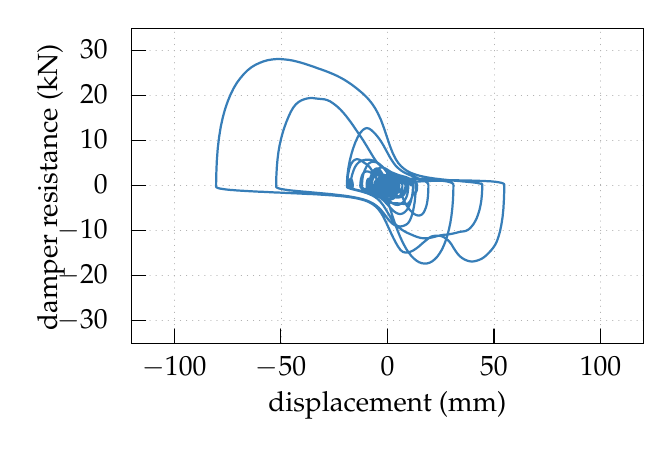
\begin{tikzpicture}[gnuplot]
%% generated with GNUPLOT 5.2p8 (Lua 5.3; terminal rev. Nov 2018, script rev. 108)
%% 08/29/2020 01:50:03
\path (0.000,0.000) rectangle (6.500,4.000);
\gpcolor{color=gp lt color axes}
\gpsetlinetype{gp lt axes}
\gpsetdashtype{gp dt axes}
\gpsetlinewidth{0.50}
\draw[gp path] (0.000,0.286)--(6.499,0.286);
\gpcolor{color=gp lt color border}
\gpsetlinetype{gp lt border}
\gpsetdashtype{gp dt solid}
\gpsetlinewidth{1.00}
\draw[gp path] (0.000,0.286)--(0.180,0.286);
\node[gp node right] at (-0.184,0.286) {$-30$};
\gpcolor{color=gp lt color axes}
\gpsetlinetype{gp lt axes}
\gpsetdashtype{gp dt axes}
\gpsetlinewidth{0.50}
\draw[gp path] (0.000,0.857)--(6.499,0.857);
\gpcolor{color=gp lt color border}
\gpsetlinetype{gp lt border}
\gpsetdashtype{gp dt solid}
\gpsetlinewidth{1.00}
\draw[gp path] (0.000,0.857)--(0.180,0.857);
\node[gp node right] at (-0.184,0.857) {$-20$};
\gpcolor{color=gp lt color axes}
\gpsetlinetype{gp lt axes}
\gpsetdashtype{gp dt axes}
\gpsetlinewidth{0.50}
\draw[gp path] (0.000,1.428)--(6.499,1.428);
\gpcolor{color=gp lt color border}
\gpsetlinetype{gp lt border}
\gpsetdashtype{gp dt solid}
\gpsetlinewidth{1.00}
\draw[gp path] (0.000,1.428)--(0.180,1.428);
\node[gp node right] at (-0.184,1.428) {$-10$};
\gpcolor{color=gp lt color axes}
\gpsetlinetype{gp lt axes}
\gpsetdashtype{gp dt axes}
\gpsetlinewidth{0.50}
\draw[gp path] (0.000,2.000)--(6.499,2.000);
\gpcolor{color=gp lt color border}
\gpsetlinetype{gp lt border}
\gpsetdashtype{gp dt solid}
\gpsetlinewidth{1.00}
\draw[gp path] (0.000,2.000)--(0.180,2.000);
\node[gp node right] at (-0.184,2.000) {$0$};
\gpcolor{color=gp lt color axes}
\gpsetlinetype{gp lt axes}
\gpsetdashtype{gp dt axes}
\gpsetlinewidth{0.50}
\draw[gp path] (0.000,2.571)--(6.499,2.571);
\gpcolor{color=gp lt color border}
\gpsetlinetype{gp lt border}
\gpsetdashtype{gp dt solid}
\gpsetlinewidth{1.00}
\draw[gp path] (0.000,2.571)--(0.180,2.571);
\node[gp node right] at (-0.184,2.571) {$10$};
\gpcolor{color=gp lt color axes}
\gpsetlinetype{gp lt axes}
\gpsetdashtype{gp dt axes}
\gpsetlinewidth{0.50}
\draw[gp path] (0.000,3.142)--(6.499,3.142);
\gpcolor{color=gp lt color border}
\gpsetlinetype{gp lt border}
\gpsetdashtype{gp dt solid}
\gpsetlinewidth{1.00}
\draw[gp path] (0.000,3.142)--(0.180,3.142);
\node[gp node right] at (-0.184,3.142) {$20$};
\gpcolor{color=gp lt color axes}
\gpsetlinetype{gp lt axes}
\gpsetdashtype{gp dt axes}
\gpsetlinewidth{0.50}
\draw[gp path] (0.000,3.713)--(6.499,3.713);
\gpcolor{color=gp lt color border}
\gpsetlinetype{gp lt border}
\gpsetdashtype{gp dt solid}
\gpsetlinewidth{1.00}
\draw[gp path] (0.000,3.713)--(0.180,3.713);
\node[gp node right] at (-0.184,3.713) {$30$};
\gpcolor{color=gp lt color axes}
\gpsetlinetype{gp lt axes}
\gpsetdashtype{gp dt axes}
\gpsetlinewidth{0.50}
\draw[gp path] (0.542,0.000)--(0.542,3.999);
\gpcolor{color=gp lt color border}
\gpsetlinetype{gp lt border}
\gpsetdashtype{gp dt solid}
\gpsetlinewidth{1.00}
\draw[gp path] (0.542,0.000)--(0.542,0.180);
\node[gp node center] at (0.542,-0.308) {$-100$};
\gpcolor{color=gp lt color axes}
\gpsetlinetype{gp lt axes}
\gpsetdashtype{gp dt axes}
\gpsetlinewidth{0.50}
\draw[gp path] (1.896,0.000)--(1.896,3.999);
\gpcolor{color=gp lt color border}
\gpsetlinetype{gp lt border}
\gpsetdashtype{gp dt solid}
\gpsetlinewidth{1.00}
\draw[gp path] (1.896,0.000)--(1.896,0.180);
\node[gp node center] at (1.896,-0.308) {$-50$};
\gpcolor{color=gp lt color axes}
\gpsetlinetype{gp lt axes}
\gpsetdashtype{gp dt axes}
\gpsetlinewidth{0.50}
\draw[gp path] (3.250,0.000)--(3.250,3.999);
\gpcolor{color=gp lt color border}
\gpsetlinetype{gp lt border}
\gpsetdashtype{gp dt solid}
\gpsetlinewidth{1.00}
\draw[gp path] (3.250,0.000)--(3.250,0.180);
\node[gp node center] at (3.250,-0.308) {$0$};
\gpcolor{color=gp lt color axes}
\gpsetlinetype{gp lt axes}
\gpsetdashtype{gp dt axes}
\gpsetlinewidth{0.50}
\draw[gp path] (4.603,0.000)--(4.603,3.999);
\gpcolor{color=gp lt color border}
\gpsetlinetype{gp lt border}
\gpsetdashtype{gp dt solid}
\gpsetlinewidth{1.00}
\draw[gp path] (4.603,0.000)--(4.603,0.180);
\node[gp node center] at (4.603,-0.308) {$50$};
\gpcolor{color=gp lt color axes}
\gpsetlinetype{gp lt axes}
\gpsetdashtype{gp dt axes}
\gpsetlinewidth{0.50}
\draw[gp path] (5.957,0.000)--(5.957,3.999);
\gpcolor{color=gp lt color border}
\gpsetlinetype{gp lt border}
\gpsetdashtype{gp dt solid}
\gpsetlinewidth{1.00}
\draw[gp path] (5.957,0.000)--(5.957,0.180);
\node[gp node center] at (5.957,-0.308) {$100$};
\draw[gp path] (0.000,3.999)--(0.000,0.000)--(6.499,0.000)--(6.499,3.999)--cycle;
\node[gp node center,rotate=-270] at (-1.028,1.999) {damper resistance (\si{\kilo\newton})};
\node[gp node center] at (3.249,-0.769) {displacement (\si{\milli\meter})};
\gpcolor{rgb color={0.216,0.494,0.722}}
\gpsetlinewidth{2.00}
\draw[gp path] (3.250,2.000)--(3.250,1.999)--(3.249,1.999)--(3.249,1.998)--(3.249,1.997)%
  --(3.249,1.996)--(3.249,1.995)--(3.248,1.994)--(3.248,1.993)--(3.247,1.991)--(3.247,1.990)%
  --(3.246,1.989)--(3.246,1.987)--(3.245,1.986)--(3.244,1.984)--(3.243,1.983)--(3.242,1.982)%
  --(3.241,1.980)--(3.240,1.979)--(3.238,1.977)--(3.237,1.976)--(3.236,1.974)--(3.234,1.973)%
  --(3.232,1.971)--(3.231,1.970)--(3.229,1.968)--(3.227,1.967)--(3.224,1.965)--(3.222,1.964)%
  --(3.220,1.963)--(3.217,1.961)--(3.215,1.960)--(3.212,1.959)--(3.210,1.959)--(3.207,1.958)%
  --(3.204,1.957)--(3.201,1.957)--(3.198,1.956)--(3.195,1.956)--(3.192,1.956)--(3.188,1.955)%
  --(3.185,1.955)--(3.182,1.955)--(3.178,1.955)--(3.175,1.955)--(3.172,1.955)--(3.168,1.955)%
  --(3.164,1.956)--(3.161,1.956)--(3.157,1.957)--(3.154,1.957)--(3.150,1.958)--(3.147,1.959)%
  --(3.143,1.960)--(3.140,1.960)--(3.137,1.961)--(3.133,1.962)--(3.130,1.963)--(3.127,1.963)%
  --(3.123,1.964)--(3.120,1.964)--(3.117,1.965)--(3.114,1.965)--(3.111,1.966)--(3.108,1.966)%
  --(3.104,1.967)--(3.101,1.967)--(3.098,1.967)--(3.095,1.968)--(3.092,1.968)--(3.089,1.968)%
  --(3.086,1.969)--(3.083,1.969)--(3.080,1.969)--(3.077,1.970)--(3.074,1.970)--(3.071,1.971)%
  --(3.068,1.971)--(3.065,1.972)--(3.062,1.973)--(3.060,1.974)--(3.058,1.976)--(3.055,1.979)%
  --(3.054,1.982)--(3.052,1.986)--(3.052,1.991)--(3.051,1.998)--(3.051,2.008)--(3.052,2.021)%
  --(3.053,2.036)--(3.055,2.051)--(3.058,2.065)--(3.061,2.080)--(3.064,2.093)--(3.068,2.106)%
  --(3.073,2.119)--(3.078,2.132)--(3.083,2.144)--(3.089,2.155)--(3.096,2.166)--(3.103,2.177)%
  --(3.110,2.188)--(3.118,2.198)--(3.127,2.207)--(3.136,2.215)--(3.145,2.221)--(3.155,2.226)%
  --(3.165,2.229)--(3.176,2.230)--(3.187,2.229)--(3.198,2.227)--(3.209,2.223)--(3.220,2.219)%
  --(3.232,2.213)--(3.244,2.206)--(3.256,2.198)--(3.268,2.190)--(3.281,2.182)--(3.294,2.173)%
  --(3.306,2.164)--(3.319,2.156)--(3.332,2.147)--(3.345,2.139)--(3.358,2.132)--(3.371,2.125)%
  --(3.384,2.118)--(3.397,2.112)--(3.410,2.106)--(3.423,2.100)--(3.436,2.095)--(3.448,2.091)%
  --(3.461,2.086)--(3.473,2.082)--(3.485,2.078)--(3.497,2.074)--(3.508,2.071)--(3.520,2.068)%
  --(3.531,2.066)--(3.542,2.063)--(3.553,2.061)--(3.564,2.059)--(3.575,2.058)--(3.585,2.056)%
  --(3.596,2.055)--(3.607,2.055)--(3.617,2.054)--(3.628,2.054)--(3.639,2.053)--(3.651,2.053)%
  --(3.662,2.053)--(3.674,2.054)--(3.686,2.054)--(3.699,2.055)--(3.712,2.055)--(3.726,2.056)%
  --(3.740,2.057)--(3.755,2.057)--(3.770,2.058)--(3.786,2.059)--(3.803,2.060)--(3.820,2.061)%
  --(3.839,2.061)--(3.858,2.062)--(3.877,2.062)--(3.897,2.062)--(3.918,2.062)--(3.939,2.062)%
  --(3.960,2.060)--(3.981,2.057)--(4.001,2.054)--(4.019,2.050)--(4.036,2.046)--(4.051,2.041)%
  --(4.064,2.036)--(4.074,2.031)--(4.082,2.025)--(4.087,2.018)--(4.088,1.998)--(4.087,1.917)%
  --(4.082,1.812)--(4.074,1.710)--(4.063,1.616)--(4.049,1.528)--(4.032,1.447)--(4.013,1.372)%
  --(3.991,1.304)--(3.967,1.241)--(3.941,1.186)--(3.913,1.139)--(3.884,1.099)--(3.853,1.066)%
  --(3.821,1.040)--(3.788,1.022)--(3.754,1.012)--(3.720,1.010)--(3.686,1.015)--(3.652,1.027)%
  --(3.618,1.048)--(3.585,1.075)--(3.552,1.109)--(3.521,1.149)--(3.490,1.195)--(3.461,1.247)%
  --(3.433,1.303)--(3.407,1.361)--(3.382,1.421)--(3.359,1.482)--(3.338,1.542)--(3.318,1.602)%
  --(3.300,1.658)--(3.284,1.710)--(3.270,1.758)--(3.257,1.802)--(3.247,1.842)--(3.239,1.879)%
  --(3.232,1.913)--(3.228,1.944)--(3.225,1.973)--(3.224,2.004)--(3.225,2.038)--(3.228,2.070)%
  --(3.233,2.099)--(3.239,2.124)--(3.247,2.146)--(3.256,2.161)--(3.267,2.169)--(3.278,2.172)%
  --(3.290,2.171)--(3.303,2.169)--(3.316,2.164)--(3.329,2.159)--(3.344,2.153)--(3.358,2.146)%
  --(3.373,2.141)--(3.388,2.135)--(3.403,2.130)--(3.419,2.127)--(3.436,2.122)--(3.453,2.117)%
  --(3.470,2.113)--(3.487,2.108)--(3.504,2.101)--(3.521,2.093)--(3.536,2.085)--(3.551,2.076)%
  --(3.564,2.068)--(3.576,2.059)--(3.586,2.051)--(3.595,2.042)--(3.601,2.034)--(3.606,2.026)%
  --(3.609,2.017)--(3.610,2.002)--(3.609,1.961)--(3.607,1.905)--(3.602,1.847)--(3.596,1.790)%
  --(3.587,1.735)--(3.577,1.684)--(3.565,1.638)--(3.551,1.596)--(3.536,1.560)--(3.520,1.534)%
  --(3.503,1.515)--(3.485,1.503)--(3.466,1.494)--(3.447,1.487)--(3.427,1.483)--(3.406,1.482)%
  --(3.386,1.485)--(3.364,1.490)--(3.342,1.498)--(3.320,1.512)--(3.296,1.532)--(3.272,1.558)%
  --(3.247,1.589)--(3.222,1.623)--(3.195,1.658)--(3.168,1.691)--(3.139,1.720)--(3.109,1.745)%
  --(3.078,1.767)--(3.046,1.785)--(3.013,1.801)--(2.978,1.814)--(2.942,1.826)--(2.906,1.835)%
  --(2.868,1.844)--(2.828,1.852)--(2.788,1.859)--(2.748,1.866)--(2.706,1.872)--(2.663,1.877)%
  --(2.620,1.882)--(2.577,1.887)--(2.533,1.892)--(2.489,1.896)--(2.445,1.900)--(2.401,1.904)%
  --(2.358,1.908)--(2.314,1.912)--(2.272,1.916)--(2.231,1.920)--(2.190,1.923)--(2.151,1.927)%
  --(2.113,1.930)--(2.076,1.934)--(2.042,1.937)--(2.009,1.941)--(1.978,1.945)--(1.949,1.949)%
  --(1.924,1.953)--(1.901,1.957)--(1.881,1.962)--(1.865,1.967)--(1.852,1.972)--(1.843,1.977)%
  --(1.838,1.983)--(1.837,2.013)--(1.839,2.112)--(1.845,2.227)--(1.854,2.331)--(1.866,2.427)%
  --(1.881,2.514)--(1.899,2.594)--(1.919,2.669)--(1.942,2.741)--(1.967,2.810)--(1.995,2.877)%
  --(2.024,2.940)--(2.055,2.992)--(2.088,3.034)--(2.123,3.063)--(2.158,3.083)--(2.194,3.097)%
  --(2.230,3.107)--(2.266,3.112)--(2.303,3.112)--(2.340,3.107)--(2.376,3.103)--(2.413,3.100)%
  --(2.450,3.096)--(2.486,3.086)--(2.522,3.070)--(2.557,3.047)--(2.592,3.021)--(2.626,2.992)%
  --(2.659,2.960)--(2.691,2.925)--(2.722,2.888)--(2.751,2.850)--(2.780,2.812)--(2.807,2.774)%
  --(2.833,2.736)--(2.858,2.699)--(2.882,2.664)--(2.905,2.631)--(2.926,2.600)--(2.947,2.568)%
  --(2.967,2.535)--(2.986,2.504)--(3.004,2.474)--(3.021,2.446)--(3.037,2.419)--(3.053,2.393)%
  --(3.067,2.369)--(3.081,2.347)--(3.095,2.327)--(3.108,2.309)--(3.120,2.293)--(3.132,2.280)%
  --(3.144,2.268)--(3.155,2.258)--(3.166,2.250)--(3.178,2.242)--(3.189,2.234)--(3.200,2.225)%
  --(3.211,2.217)--(3.223,2.207)--(3.234,2.197)--(3.245,2.187)--(3.256,2.177)--(3.266,2.168)%
  --(3.277,2.159)--(3.288,2.151)--(3.299,2.142)--(3.309,2.135)--(3.320,2.128)--(3.330,2.122)%
  --(3.341,2.116)--(3.351,2.111)--(3.362,2.107)--(3.373,2.104)--(3.383,2.101)--(3.394,2.098)%
  --(3.406,2.096)--(3.417,2.095)--(3.429,2.093)--(3.442,2.093)--(3.454,2.092)--(3.467,2.091)%
  --(3.481,2.091)--(3.496,2.090)--(3.510,2.090)--(3.526,2.089)--(3.542,2.089)--(3.559,2.089)%
  --(3.576,2.088)--(3.594,2.087)--(3.613,2.087)--(3.632,2.086)--(3.652,2.085)--(3.672,2.084)%
  --(3.694,2.083)--(3.715,2.082)--(3.737,2.081)--(3.760,2.080)--(3.784,2.079)--(3.807,2.078)%
  --(3.832,2.077)--(3.856,2.076)--(3.881,2.075)--(3.907,2.074)--(3.933,2.073)--(3.960,2.072)%
  --(3.987,2.071)--(4.014,2.070)--(4.042,2.070)--(4.070,2.069)--(4.099,2.068)--(4.128,2.068)%
  --(4.158,2.067)--(4.188,2.066)--(4.219,2.066)--(4.250,2.065)--(4.282,2.065)--(4.314,2.064)%
  --(4.346,2.063)--(4.378,2.062)--(4.411,2.061)--(4.443,2.060)--(4.476,2.059)--(4.507,2.057)%
  --(4.539,2.056)--(4.570,2.054)--(4.600,2.051)--(4.627,2.048)--(4.652,2.044)--(4.675,2.040)%
  --(4.694,2.036)--(4.710,2.031)--(4.722,2.026)--(4.730,2.021)--(4.734,2.014)--(4.734,1.952)%
  --(4.730,1.832)--(4.723,1.707)--(4.712,1.598)--(4.697,1.502)--(4.680,1.419)--(4.660,1.349)%
  --(4.639,1.290)--(4.615,1.243)--(4.590,1.206)--(4.564,1.175)--(4.537,1.146)--(4.509,1.118)%
  --(4.480,1.093)--(4.450,1.073)--(4.420,1.059)--(4.389,1.048)--(4.358,1.040)--(4.327,1.036)%
  --(4.295,1.039)--(4.264,1.047)--(4.233,1.060)--(4.202,1.078)--(4.172,1.101)--(4.143,1.132)%
  --(4.116,1.169)--(4.089,1.211)--(4.064,1.253)--(4.040,1.285)--(4.017,1.309)--(3.994,1.327)%
  --(3.972,1.342)--(3.951,1.353)--(3.929,1.360)--(3.908,1.363)--(3.887,1.363)--(3.866,1.363)%
  --(3.844,1.362)--(3.823,1.358)--(3.801,1.350)--(3.779,1.336)--(3.756,1.318)--(3.733,1.299)%
  --(3.708,1.279)--(3.683,1.257)--(3.657,1.234)--(3.630,1.212)--(3.602,1.192)--(3.573,1.174)%
  --(3.543,1.161)--(3.512,1.151)--(3.481,1.150)--(3.449,1.157)--(3.416,1.182)--(3.384,1.228)%
  --(3.352,1.283)--(3.321,1.344)--(3.290,1.410)--(3.259,1.478)--(3.228,1.545)--(3.197,1.607)%
  --(3.166,1.659)--(3.134,1.701)--(3.102,1.734)--(3.068,1.760)--(3.034,1.781)--(2.998,1.798)%
  --(2.962,1.812)--(2.924,1.823)--(2.884,1.833)--(2.843,1.842)--(2.801,1.849)--(2.757,1.855)%
  --(2.712,1.861)--(2.666,1.866)--(2.618,1.870)--(2.568,1.875)--(2.517,1.878)--(2.465,1.882)%
  --(2.412,1.885)--(2.357,1.889)--(2.301,1.892)--(2.244,1.894)--(2.187,1.897)--(2.128,1.900)%
  --(2.069,1.903)--(2.010,1.905)--(1.950,1.908)--(1.890,1.911)--(1.830,1.913)--(1.771,1.916)%
  --(1.712,1.919)--(1.654,1.922)--(1.598,1.924)--(1.542,1.927)--(1.488,1.930)--(1.436,1.933)%
  --(1.386,1.936)--(1.338,1.939)--(1.293,1.943)--(1.251,1.946)--(1.213,1.950)--(1.178,1.954)%
  --(1.148,1.959)--(1.123,1.963)--(1.102,1.968)--(1.087,1.974)--(1.078,1.980)--(1.074,1.992)%
  --(1.076,2.130)--(1.083,2.309)--(1.095,2.472)--(1.113,2.622)--(1.135,2.756)--(1.161,2.873)%
  --(1.190,2.978)--(1.223,3.073)--(1.259,3.160)--(1.298,3.239)--(1.339,3.307)--(1.383,3.366)%
  --(1.428,3.419)--(1.476,3.466)--(1.524,3.504)--(1.574,3.534)--(1.625,3.558)--(1.677,3.578)%
  --(1.730,3.593)--(1.783,3.602)--(1.836,3.607)--(1.889,3.607)--(1.943,3.603)--(1.996,3.597)%
  --(2.049,3.588)--(2.102,3.575)--(2.155,3.561)--(2.207,3.545)--(2.258,3.528)--(2.309,3.511)%
  --(2.360,3.492)--(2.410,3.475)--(2.460,3.457)--(2.509,3.438)--(2.557,3.418)--(2.606,3.396)%
  --(2.653,3.372)--(2.700,3.346)--(2.746,3.317)--(2.792,3.286)--(2.836,3.253)--(2.880,3.218)%
  --(2.923,3.182)--(2.966,3.143)--(3.008,3.099)--(3.049,3.049)--(3.090,2.989)--(3.129,2.919)%
  --(3.169,2.832)--(3.207,2.729)--(3.245,2.615)--(3.282,2.504)--(3.318,2.412)--(3.353,2.341)%
  --(3.387,2.288)--(3.422,2.248)--(3.456,2.218)--(3.489,2.194)--(3.522,2.175)--(3.555,2.159)%
  --(3.588,2.147)--(3.621,2.136)--(3.653,2.127)--(3.685,2.119)--(3.717,2.112)--(3.749,2.106)%
  --(3.780,2.100)--(3.811,2.096)--(3.842,2.091)--(3.872,2.087)--(3.902,2.084)--(3.932,2.080)%
  --(3.961,2.077)--(3.990,2.074)--(4.018,2.071)--(4.046,2.068)--(4.073,2.066)--(4.100,2.063)%
  --(4.126,2.061)--(4.152,2.059)--(4.177,2.057)--(4.201,2.054)--(4.224,2.052)--(4.247,2.050)%
  --(4.268,2.048)--(4.289,2.046)--(4.309,2.044)--(4.327,2.042)--(4.345,2.040)--(4.361,2.038)%
  --(4.377,2.036)--(4.391,2.034)--(4.404,2.031)--(4.415,2.029)--(4.425,2.027)--(4.434,2.025)%
  --(4.441,2.023)--(4.447,2.020)--(4.451,2.018)--(4.454,2.014)--(4.455,2.002)--(4.454,1.965)%
  --(4.452,1.915)--(4.448,1.864)--(4.443,1.816)--(4.436,1.771)--(4.428,1.729)--(4.419,1.691)%
  --(4.408,1.654)--(4.396,1.619)--(4.384,1.587)--(4.370,1.558)--(4.355,1.531)--(4.340,1.507)%
  --(4.323,1.486)--(4.306,1.466)--(4.289,1.450)--(4.271,1.438)--(4.252,1.428)--(4.234,1.422)%
  --(4.215,1.419)--(4.196,1.417)--(4.177,1.414)--(4.158,1.410)--(4.139,1.405)--(4.119,1.400)%
  --(4.099,1.395)--(4.080,1.391)--(4.060,1.387)--(4.039,1.383)--(4.019,1.380)--(3.999,1.378)%
  --(3.978,1.377)--(3.957,1.374)--(3.937,1.371)--(3.916,1.367)--(3.895,1.362)--(3.873,1.357)%
  --(3.852,1.351)--(3.830,1.345)--(3.808,1.340)--(3.786,1.336)--(3.763,1.333)--(3.741,1.331)%
  --(3.718,1.331)--(3.695,1.333)--(3.672,1.336)--(3.649,1.342)--(3.626,1.349)--(3.604,1.357)%
  --(3.581,1.366)--(3.559,1.376)--(3.537,1.385)--(3.515,1.395)--(3.493,1.405)--(3.471,1.417)%
  --(3.449,1.430)--(3.427,1.445)--(3.406,1.461)--(3.384,1.478)--(3.363,1.499)--(3.342,1.523)%
  --(3.320,1.550)--(3.299,1.581)--(3.279,1.614)--(3.258,1.650)--(3.238,1.684)--(3.218,1.717)%
  --(3.199,1.747)--(3.179,1.773)--(3.161,1.796)--(3.142,1.815)--(3.124,1.832)--(3.105,1.846)%
  --(3.088,1.858)--(3.070,1.868)--(3.053,1.877)--(3.036,1.885)--(3.019,1.893)--(3.002,1.899)%
  --(2.986,1.905)--(2.970,1.910)--(2.954,1.915)--(2.939,1.920)--(2.924,1.924)--(2.910,1.928)%
  --(2.896,1.932)--(2.882,1.935)--(2.869,1.938)--(2.857,1.941)--(2.845,1.944)--(2.833,1.947)%
  --(2.822,1.950)--(2.812,1.953)--(2.802,1.955)--(2.792,1.958)--(2.784,1.960)--(2.776,1.963)%
  --(2.769,1.965)--(2.762,1.968)--(2.756,1.970)--(2.751,1.973)--(2.747,1.976)--(2.743,1.980)%
  --(2.741,1.984)--(2.740,1.991)--(2.740,2.007)--(2.741,2.036)--(2.743,2.071)--(2.746,2.105)%
  --(2.750,2.138)--(2.756,2.168)--(2.762,2.197)--(2.769,2.224)--(2.777,2.248)--(2.786,2.269)%
  --(2.796,2.286)--(2.806,2.300)--(2.817,2.313)--(2.828,2.322)--(2.839,2.329)--(2.850,2.333)%
  --(2.862,2.335)--(2.874,2.334)--(2.885,2.332)--(2.897,2.328)--(2.908,2.323)--(2.920,2.316)%
  --(2.931,2.308)--(2.942,2.300)--(2.952,2.292)--(2.963,2.285)--(2.973,2.279)--(2.983,2.273)%
  --(2.993,2.266)--(3.002,2.257)--(3.012,2.248)--(3.021,2.238)--(3.030,2.227)--(3.038,2.216)%
  --(3.046,2.204)--(3.054,2.193)--(3.061,2.181)--(3.068,2.170)--(3.074,2.159)--(3.081,2.148)%
  --(3.086,2.138)--(3.092,2.127)--(3.097,2.117)--(3.101,2.108)--(3.106,2.099)--(3.110,2.090)%
  --(3.113,2.081)--(3.117,2.073)--(3.120,2.065)--(3.123,2.057)--(3.125,2.049)--(3.127,2.042)%
  --(3.129,2.035)--(3.130,2.030)--(3.132,2.024)--(3.133,2.020)--(3.134,2.017)--(3.135,2.016)%
  --(3.136,2.015)--(3.136,2.016)--(3.137,2.017)--(3.138,2.020)--(3.139,2.023)--(3.141,2.028)%
  --(3.142,2.033)--(3.144,2.039)--(3.146,2.046)--(3.148,2.053)--(3.151,2.060)--(3.154,2.067)%
  --(3.157,2.075)--(3.161,2.082)--(3.164,2.088)--(3.169,2.094)--(3.173,2.100)--(3.178,2.105)%
  --(3.183,2.109)--(3.189,2.114)--(3.194,2.118)--(3.200,2.120)--(3.206,2.119)--(3.212,2.117)%
  --(3.218,2.112)--(3.224,2.107)--(3.230,2.100)--(3.235,2.092)--(3.240,2.082)--(3.244,2.072)%
  --(3.248,2.062)--(3.252,2.051)--(3.255,2.041)--(3.257,2.030)--(3.258,2.018)--(3.259,2.007)%
  --(3.259,1.996)--(3.258,1.984)--(3.257,1.972)--(3.255,1.961)--(3.253,1.949)--(3.250,1.939)%
  --(3.246,1.929)--(3.241,1.920)--(3.236,1.912)--(3.230,1.904)--(3.224,1.898)--(3.217,1.893)%
  --(3.209,1.888)--(3.201,1.885)--(3.192,1.883)--(3.183,1.882)--(3.173,1.881)--(3.163,1.881)%
  --(3.153,1.883)--(3.142,1.884)--(3.130,1.886)--(3.118,1.889)--(3.106,1.892)--(3.094,1.895)%
  --(3.082,1.899)--(3.070,1.905)--(3.058,1.912)--(3.046,1.919)--(3.036,1.927)--(3.026,1.936)%
  --(3.018,1.944)--(3.010,1.951)--(3.004,1.957)--(2.999,1.963)--(2.994,1.968)--(2.991,1.974)%
  --(2.988,1.980)--(2.987,1.986)--(2.986,1.995)--(2.986,2.007)--(2.987,2.021)--(2.988,2.035)%
  --(2.990,2.046)--(2.992,2.056)--(2.994,2.065)--(2.997,2.072)--(3.000,2.078)--(3.003,2.082)%
  --(3.007,2.085)--(3.010,2.086)--(3.013,2.087)--(3.017,2.087)--(3.020,2.087)--(3.024,2.084)%
  --(3.027,2.085)--(3.031,2.093)--(3.035,2.104)--(3.039,2.117)--(3.044,2.130)--(3.049,2.142)%
  --(3.055,2.154)--(3.061,2.166)--(3.068,2.179)--(3.075,2.191)--(3.083,2.200)--(3.091,2.208)%
  --(3.100,2.213)--(3.108,2.217)--(3.117,2.219)--(3.126,2.217)--(3.135,2.213)--(3.145,2.206)%
  --(3.153,2.198)--(3.162,2.187)--(3.170,2.174)--(3.178,2.162)--(3.185,2.149)--(3.192,2.137)%
  --(3.199,2.125)--(3.205,2.114)--(3.210,2.103)--(3.215,2.093)--(3.220,2.084)--(3.224,2.077)%
  --(3.228,2.073)--(3.233,2.073)--(3.237,2.074)--(3.241,2.074)--(3.245,2.073)--(3.249,2.071)%
  --(3.254,2.070)--(3.258,2.069)--(3.262,2.068)--(3.266,2.067)--(3.271,2.065)--(3.275,2.064)%
  --(3.279,2.063)--(3.283,2.063)--(3.288,2.063)--(3.292,2.063)--(3.296,2.063)--(3.301,2.063)%
  --(3.306,2.063)--(3.310,2.062)--(3.315,2.062)--(3.320,2.061)--(3.325,2.060)--(3.330,2.059)%
  --(3.334,2.058)--(3.339,2.057)--(3.344,2.057)--(3.349,2.056)--(3.354,2.055)--(3.359,2.054)%
  --(3.364,2.053)--(3.369,2.052)--(3.374,2.052)--(3.379,2.051)--(3.384,2.051)--(3.389,2.051)%
  --(3.395,2.051)--(3.400,2.051)--(3.406,2.051)--(3.411,2.052)--(3.417,2.052)--(3.423,2.053)%
  --(3.430,2.053)--(3.436,2.053)--(3.443,2.054)--(3.449,2.054)--(3.456,2.054)--(3.464,2.054)%
  --(3.471,2.054)--(3.478,2.054)--(3.486,2.053)--(3.494,2.053)--(3.501,2.052)--(3.509,2.051)%
  --(3.517,2.051)--(3.525,2.050)--(3.533,2.049)--(3.540,2.048)--(3.548,2.047)--(3.556,2.046)%
  --(3.563,2.045)--(3.571,2.043)--(3.578,2.042)--(3.585,2.041)--(3.592,2.039)--(3.598,2.037)%
  --(3.604,2.034)--(3.610,2.032)--(3.615,2.029)--(3.619,2.025)--(3.622,2.022)--(3.625,2.018)%
  --(3.626,2.013)--(3.627,2.006)--(3.627,1.994)--(3.627,1.978)--(3.625,1.961)--(3.624,1.946)%
  --(3.621,1.935)--(3.619,1.929)--(3.616,1.922)--(3.613,1.916)--(3.610,1.912)--(3.606,1.909)%
  --(3.603,1.907)--(3.599,1.906)--(3.596,1.906)--(3.592,1.906)--(3.589,1.905)--(3.585,1.904)%
  --(3.582,1.901)--(3.578,1.896)--(3.574,1.888)--(3.569,1.876)--(3.565,1.864)--(3.559,1.850)%
  --(3.554,1.836)--(3.547,1.822)--(3.541,1.809)--(3.534,1.797)--(3.526,1.787)--(3.518,1.778)%
  --(3.510,1.772)--(3.501,1.767)--(3.493,1.765)--(3.484,1.764)--(3.475,1.765)--(3.466,1.766)%
  --(3.457,1.767)--(3.449,1.768)--(3.440,1.770)--(3.431,1.771)--(3.422,1.772)--(3.413,1.773)%
  --(3.404,1.773)--(3.395,1.774)--(3.385,1.775)--(3.376,1.775)--(3.367,1.776)--(3.357,1.776)%
  --(3.348,1.777)--(3.338,1.777)--(3.328,1.777)--(3.317,1.778)--(3.307,1.779)--(3.296,1.782)%
  --(3.285,1.787)--(3.274,1.792)--(3.263,1.799)--(3.251,1.807)--(3.240,1.815)--(3.228,1.823)%
  --(3.217,1.831)--(3.205,1.839)--(3.193,1.846)--(3.181,1.853)--(3.169,1.860)--(3.157,1.866)%
  --(3.145,1.872)--(3.133,1.877)--(3.120,1.882)--(3.108,1.887)--(3.095,1.891)--(3.082,1.895)%
  --(3.069,1.898)--(3.055,1.902)--(3.042,1.905)--(3.029,1.908)--(3.015,1.911)--(3.001,1.914)%
  --(2.988,1.918)--(2.974,1.921)--(2.961,1.924)--(2.947,1.927)--(2.934,1.930)--(2.921,1.932)%
  --(2.909,1.935)--(2.896,1.938)--(2.884,1.941)--(2.873,1.943)--(2.861,1.946)--(2.851,1.948)%
  --(2.840,1.951)--(2.830,1.953)--(2.821,1.956)--(2.812,1.958)--(2.804,1.961)--(2.796,1.963)%
  --(2.789,1.966)--(2.783,1.969)--(2.778,1.971)--(2.773,1.974)--(2.769,1.976)--(2.766,1.979)%
  --(2.763,1.982)--(2.761,1.985)--(2.760,1.990)--(2.760,1.998)--(2.760,2.009)--(2.761,2.023)%
  --(2.762,2.036)--(2.764,2.048)--(2.766,2.058)--(2.768,2.067)--(2.771,2.073)--(2.774,2.078)%
  --(2.777,2.082)--(2.780,2.084)--(2.783,2.085)--(2.786,2.084)--(2.789,2.082)--(2.792,2.079)%
  --(2.795,2.074)--(2.798,2.069)--(2.800,2.062)--(2.803,2.054)--(2.805,2.046)--(2.806,2.036)%
  --(2.808,2.027)--(2.809,2.017)--(2.809,2.007)--(2.809,1.999)--(2.809,1.993)--(2.808,1.988)%
  --(2.807,1.985)--(2.805,1.983)--(2.803,1.980)--(2.801,1.978)--(2.797,1.976)--(2.793,1.974)%
  --(2.789,1.973)--(2.784,1.971)--(2.779,1.970)--(2.773,1.969)--(2.767,1.969)--(2.761,1.969)%
  --(2.756,1.970)--(2.750,1.972)--(2.745,1.974)--(2.741,1.977)--(2.738,1.980)--(2.736,1.986)%
  --(2.735,1.998)--(2.736,2.028)--(2.738,2.072)--(2.741,2.120)--(2.747,2.169)--(2.753,2.217)%
  --(2.762,2.265)--(2.771,2.314)--(2.783,2.362)--(2.796,2.412)--(2.811,2.461)--(2.828,2.510)%
  --(2.846,2.558)--(2.867,2.603)--(2.888,2.644)--(2.912,2.678)--(2.936,2.705)--(2.962,2.723)%
  --(2.988,2.731)--(3.015,2.725)--(3.042,2.708)--(3.069,2.684)--(3.096,2.657)--(3.122,2.626)%
  --(3.148,2.592)--(3.174,2.553)--(3.200,2.510)--(3.225,2.464)--(3.251,2.417)--(3.276,2.370)%
  --(3.302,2.327)--(3.328,2.289)--(3.353,2.256)--(3.379,2.229)--(3.405,2.207)--(3.431,2.187)%
  --(3.457,2.171)--(3.483,2.157)--(3.509,2.145)--(3.535,2.134)--(3.560,2.124)--(3.585,2.114)%
  --(3.609,2.105)--(3.632,2.096)--(3.653,2.088)--(3.674,2.080)--(3.692,2.072)--(3.710,2.064)%
  --(3.725,2.057)--(3.738,2.050)--(3.749,2.042)--(3.758,2.035)--(3.764,2.027)--(3.768,2.020)%
  --(3.770,2.009)--(3.770,1.971)--(3.768,1.914)--(3.764,1.857)--(3.758,1.808)--(3.751,1.767)%
  --(3.742,1.733)--(3.732,1.705)--(3.722,1.681)--(3.711,1.660)--(3.699,1.644)--(3.686,1.632)%
  --(3.674,1.626)--(3.661,1.622)--(3.648,1.621)--(3.635,1.621)--(3.621,1.625)--(3.608,1.630)%
  --(3.596,1.637)--(3.583,1.645)--(3.571,1.655)--(3.559,1.666)--(3.547,1.678)--(3.535,1.690)%
  --(3.524,1.704)--(3.514,1.718)--(3.504,1.733)--(3.494,1.748)--(3.485,1.763)--(3.477,1.778)%
  --(3.469,1.794)--(3.461,1.810)--(3.454,1.825)--(3.448,1.840)--(3.442,1.855)--(3.436,1.869)%
  --(3.431,1.883)--(3.427,1.896)--(3.423,1.908)--(3.420,1.920)--(3.416,1.929)--(3.414,1.937)%
  --(3.411,1.944)--(3.409,1.951)--(3.407,1.956)--(3.405,1.961)--(3.403,1.965)--(3.402,1.967)%
  --(3.400,1.969)--(3.399,1.969)--(3.397,1.967)--(3.396,1.965)--(3.394,1.962)--(3.393,1.958)%
  --(3.391,1.955)--(3.389,1.951)--(3.386,1.949)--(3.384,1.947)--(3.382,1.946)--(3.379,1.945)%
  --(3.377,1.946)--(3.374,1.947)--(3.372,1.949)--(3.370,1.952)--(3.368,1.955)--(3.366,1.959)%
  --(3.364,1.964)--(3.363,1.968)--(3.361,1.971)--(3.360,1.975)--(3.359,1.979)--(3.358,1.982)%
  --(3.357,1.986)--(3.356,1.989)--(3.356,1.992)--(3.355,1.996)--(3.355,1.999)--(3.355,2.002)%
  --(3.356,2.005)--(3.356,2.008)--(3.357,2.011)--(3.358,2.014)--(3.359,2.017)--(3.360,2.020)%
  --(3.362,2.023)--(3.364,2.026)--(3.366,2.029)--(3.369,2.032)--(3.372,2.036)--(3.375,2.039)%
  --(3.379,2.042)--(3.383,2.044)--(3.388,2.047)--(3.393,2.049)--(3.398,2.051)--(3.404,2.053)%
  --(3.410,2.054)--(3.416,2.055)--(3.422,2.056)--(3.429,2.056)--(3.435,2.055)--(3.442,2.054)%
  --(3.449,2.053)--(3.456,2.051)--(3.462,2.049)--(3.469,2.047)--(3.475,2.046)--(3.481,2.044)%
  --(3.486,2.041)--(3.492,2.038)--(3.496,2.035)--(3.501,2.031)--(3.505,2.028)--(3.508,2.025)%
  --(3.510,2.021)--(3.512,2.018)--(3.514,2.014)--(3.515,2.010)--(3.515,2.004)--(3.515,1.993)%
  --(3.515,1.978)--(3.513,1.959)--(3.511,1.939)--(3.509,1.919)--(3.505,1.901)--(3.501,1.884)%
  --(3.496,1.868)--(3.491,1.854)--(3.485,1.841)--(3.479,1.830)--(3.472,1.820)--(3.465,1.811)%
  --(3.458,1.802)--(3.450,1.793)--(3.442,1.785)--(3.434,1.778)--(3.425,1.772)--(3.416,1.767)%
  --(3.407,1.762)--(3.397,1.759)--(3.387,1.756)--(3.377,1.755)--(3.367,1.756)--(3.357,1.757)%
  --(3.346,1.760)--(3.336,1.764)--(3.325,1.770)--(3.314,1.776)--(3.304,1.784)--(3.293,1.792)%
  --(3.283,1.802)--(3.273,1.812)--(3.263,1.823)--(3.253,1.834)--(3.243,1.846)--(3.234,1.857)%
  --(3.225,1.867)--(3.217,1.877)--(3.208,1.885)--(3.200,1.893)--(3.193,1.899)--(3.185,1.905)%
  --(3.178,1.909)--(3.170,1.914)--(3.163,1.918)--(3.156,1.921)--(3.150,1.924)--(3.143,1.927)%
  --(3.136,1.929)--(3.129,1.932)--(3.123,1.934)--(3.116,1.935)--(3.109,1.937)--(3.103,1.939)%
  --(3.096,1.940)--(3.090,1.942)--(3.084,1.943)--(3.077,1.945)--(3.071,1.946)--(3.064,1.947)%
  --(3.058,1.948)--(3.052,1.949)--(3.046,1.950)--(3.039,1.951)--(3.033,1.952)--(3.027,1.952)%
  --(3.021,1.953)--(3.014,1.953)--(3.008,1.953)--(3.001,1.954)--(2.995,1.954)--(2.988,1.954)%
  --(2.982,1.954)--(2.975,1.955)--(2.968,1.956)--(2.962,1.956)--(2.955,1.957)--(2.949,1.960)%
  --(2.943,1.963)--(2.938,1.968)--(2.934,1.972)--(2.931,1.978)--(2.929,1.984)--(2.928,1.994)%
  --(2.928,2.015)--(2.929,2.042)--(2.931,2.070)--(2.934,2.096)--(2.938,2.120)--(2.943,2.142)%
  --(2.949,2.161)--(2.955,2.179)--(2.962,2.197)--(2.970,2.214)--(2.978,2.230)--(2.986,2.246)%
  --(2.996,2.260)--(3.006,2.272)--(3.016,2.282)--(3.027,2.290)--(3.038,2.296)--(3.049,2.300)%
  --(3.060,2.302)--(3.072,2.302)--(3.084,2.301)--(3.096,2.299)--(3.108,2.295)--(3.120,2.290)%
  --(3.132,2.284)--(3.144,2.277)--(3.156,2.268)--(3.168,2.258)--(3.179,2.247)--(3.191,2.235)%
  --(3.202,2.223)--(3.213,2.209)--(3.224,2.195)--(3.234,2.182)--(3.244,2.168)--(3.254,2.155)%
  --(3.263,2.143)--(3.272,2.131)--(3.280,2.120)--(3.288,2.110)--(3.296,2.101)--(3.303,2.093)%
  --(3.309,2.085)--(3.316,2.078)--(3.322,2.072)--(3.327,2.066)--(3.333,2.060)--(3.338,2.056)%
  --(3.342,2.052)--(3.346,2.048)--(3.350,2.044)--(3.354,2.040)--(3.357,2.037)--(3.360,2.033)%
  --(3.363,2.029)--(3.365,2.025)--(3.367,2.021)--(3.369,2.017)--(3.370,2.013)--(3.371,2.009)%
  --(3.371,2.005)--(3.371,2.001)--(3.371,1.997)--(3.371,1.994)--(3.371,1.990)--(3.370,1.987)%
  --(3.369,1.984)--(3.369,1.981)--(3.368,1.978)--(3.367,1.976)--(3.365,1.974)--(3.364,1.973)%
  --(3.363,1.972)--(3.361,1.972)--(3.360,1.973)--(3.359,1.975)--(3.358,1.977)--(3.357,1.980)%
  --(3.356,1.984)--(3.355,1.988)--(3.355,1.992)--(3.354,1.996)--(3.354,2.000)--(3.354,2.004)%
  --(3.355,2.007)--(3.355,2.010)--(3.356,2.013)--(3.357,2.015)--(3.359,2.018)--(3.360,2.020)%
  --(3.362,2.022)--(3.364,2.023)--(3.366,2.025)--(3.368,2.027)--(3.370,2.028)--(3.372,2.029)%
  --(3.375,2.030)--(3.378,2.031)--(3.381,2.031)--(3.383,2.030)--(3.386,2.029)--(3.389,2.027)%
  --(3.391,2.025)--(3.393,2.022)--(3.395,2.019)--(3.396,2.016)--(3.397,2.013)--(3.398,2.009)%
  --(3.399,2.005)--(3.399,2.000)--(3.399,1.994)--(3.398,1.987)--(3.397,1.979)--(3.396,1.972)%
  --(3.395,1.966)--(3.393,1.961)--(3.391,1.957)--(3.390,1.955)--(3.388,1.954)--(3.386,1.955)%
  --(3.384,1.955)--(3.382,1.956)--(3.380,1.958)--(3.378,1.960)--(3.376,1.962)--(3.374,1.965)%
  --(3.373,1.968)--(3.371,1.971)--(3.370,1.975)--(3.369,1.980)--(3.368,1.985)--(3.368,1.990)%
  --(3.367,1.994)--(3.367,1.999)--(3.367,2.003)--(3.367,2.006)--(3.368,2.009)--(3.369,2.011)%
  --(3.369,2.013)--(3.371,2.014)--(3.372,2.014)--(3.373,2.014)--(3.374,2.013)--(3.374,2.012)%
  --(3.375,2.010)--(3.376,2.009)--(3.376,2.007)--(3.377,2.005)--(3.377,2.002)--(3.377,1.998)%
  --(3.377,1.993)--(3.376,1.987)--(3.376,1.979)--(3.374,1.970)--(3.373,1.961)--(3.371,1.951)%
  --(3.368,1.942)--(3.366,1.933)--(3.363,1.925)--(3.359,1.919)--(3.355,1.913)--(3.351,1.908)%
  --(3.347,1.903)--(3.343,1.899)--(3.338,1.896)--(3.333,1.893)--(3.328,1.890)--(3.323,1.887)%
  --(3.318,1.884)--(3.312,1.882)--(3.306,1.880)--(3.301,1.878)--(3.294,1.877)--(3.288,1.877)%
  --(3.282,1.878)--(3.275,1.879)--(3.269,1.881)--(3.262,1.884)--(3.256,1.888)--(3.250,1.891)%
  --(3.243,1.896)--(3.237,1.901)--(3.231,1.906)--(3.225,1.911)--(3.220,1.917)--(3.214,1.922)%
  --(3.209,1.927)--(3.204,1.931)--(3.199,1.935)--(3.195,1.938)--(3.190,1.940)--(3.186,1.943)%
  --(3.182,1.945)--(3.177,1.947)--(3.173,1.948)--(3.169,1.950)--(3.165,1.952)--(3.162,1.954)%
  --(3.158,1.955)--(3.154,1.957)--(3.151,1.959)--(3.147,1.961)--(3.144,1.962)--(3.141,1.964)%
  --(3.138,1.966)--(3.135,1.968)--(3.133,1.970)--(3.131,1.973)--(3.128,1.975)--(3.127,1.978)%
  --(3.125,1.981)--(3.124,1.985)--(3.123,1.989)--(3.122,1.993)--(3.122,1.999)--(3.122,2.005)%
  --(3.123,2.012)--(3.124,2.018)--(3.125,2.024)--(3.126,2.030)--(3.127,2.034)--(3.129,2.037)%
  --(3.131,2.039)--(3.133,2.041)--(3.135,2.042)--(3.137,2.044)--(3.139,2.044)--(3.141,2.045)%
  --(3.143,2.046)--(3.145,2.047)--(3.147,2.048)--(3.150,2.047)--(3.152,2.046)--(3.154,2.045)%
  --(3.156,2.043)--(3.158,2.041)--(3.160,2.039)--(3.162,2.036)--(3.164,2.033)--(3.165,2.030)%
  --(3.167,2.027)--(3.168,2.024)--(3.169,2.021)--(3.170,2.017)--(3.171,2.014)--(3.172,2.010)%
  --(3.172,2.007)--(3.173,2.004)--(3.173,2.001)--(3.173,1.998)--(3.173,1.996)--(3.172,1.993)%
  --(3.172,1.991)--(3.171,1.989)--(3.170,1.987)--(3.170,1.985)--(3.169,1.984)--(3.168,1.984)%
  --(3.167,1.986)--(3.166,1.988)--(3.165,1.993)--(3.165,1.998)--(3.165,2.006)--(3.166,2.016)%
  --(3.167,2.027)--(3.168,2.039)--(3.171,2.051)--(3.173,2.062)--(3.177,2.072)--(3.180,2.081)%
  --(3.184,2.089)--(3.189,2.096)--(3.194,2.101)--(3.199,2.105)--(3.204,2.108)--(3.210,2.111)%
  --(3.215,2.112)--(3.221,2.113)--(3.228,2.114)--(3.234,2.114)--(3.240,2.114)--(3.247,2.113)%
  --(3.254,2.112)--(3.260,2.111)--(3.267,2.109)--(3.274,2.107)--(3.282,2.105)--(3.289,2.102)%
  --(3.296,2.100)--(3.303,2.096)--(3.310,2.093)--(3.318,2.089)--(3.325,2.086)--(3.332,2.081)%
  --(3.339,2.076)--(3.345,2.071)--(3.351,2.066)--(3.357,2.060)--(3.362,2.054)--(3.367,2.049)%
  --(3.371,2.043)--(3.375,2.038)--(3.379,2.033)--(3.381,2.028)--(3.384,2.023)--(3.385,2.017)%
  --(3.386,2.010)--(3.387,2.001)--(3.386,1.989)--(3.386,1.975)--(3.384,1.960)--(3.382,1.945)%
  --(3.379,1.931)--(3.376,1.917)--(3.372,1.905)--(3.368,1.893)--(3.363,1.882)--(3.358,1.872)%
  --(3.352,1.862)--(3.346,1.854)--(3.339,1.847)--(3.332,1.841)--(3.324,1.835)--(3.317,1.832)%
  --(3.309,1.829)--(3.300,1.827)--(3.292,1.826)--(3.283,1.826)--(3.273,1.827)--(3.264,1.829)%
  --(3.254,1.831)--(3.244,1.835)--(3.234,1.838)--(3.224,1.843)--(3.213,1.848)--(3.203,1.853)%
  --(3.192,1.859)--(3.181,1.865)--(3.170,1.872)--(3.159,1.878)--(3.148,1.884)--(3.137,1.892)%
  --(3.127,1.899)--(3.117,1.907)--(3.107,1.914)--(3.098,1.921)--(3.089,1.928)--(3.082,1.934)%
  --(3.074,1.941)--(3.068,1.946)--(3.062,1.952)--(3.056,1.957)--(3.052,1.962)--(3.048,1.967)%
  --(3.044,1.972)--(3.042,1.977)--(3.040,1.983)--(3.039,1.990)--(3.039,2.000)--(3.039,2.013)%
  --(3.040,2.030)--(3.042,2.047)--(3.044,2.063)--(3.047,2.079)--(3.050,2.092)--(3.054,2.104)%
  --(3.059,2.115)--(3.063,2.124)--(3.069,2.131)--(3.074,2.138)--(3.080,2.143)--(3.085,2.148)%
  --(3.091,2.152)--(3.098,2.156)--(3.104,2.159)--(3.111,2.161)--(3.117,2.161)--(3.124,2.161)%
  --(3.131,2.160)--(3.138,2.158)--(3.145,2.155)--(3.151,2.152)--(3.158,2.149)--(3.165,2.145)%
  --(3.171,2.142)--(3.178,2.139)--(3.184,2.135)--(3.191,2.131)--(3.197,2.127)--(3.203,2.122)%
  --(3.209,2.117)--(3.215,2.111)--(3.221,2.105)--(3.227,2.099)--(3.232,2.094)--(3.237,2.088)%
  --(3.242,2.083)--(3.247,2.078)--(3.251,2.073)--(3.255,2.068)--(3.259,2.064)--(3.263,2.060)%
  --(3.267,2.056)--(3.270,2.052)--(3.273,2.049)--(3.277,2.046)--(3.279,2.043)--(3.282,2.040)%
  --(3.285,2.038)--(3.287,2.036)--(3.290,2.034)--(3.292,2.032)--(3.294,2.031)--(3.296,2.030)%
  --(3.298,2.029)--(3.300,2.029)--(3.302,2.029)--(3.304,2.029)--(3.306,2.029)--(3.308,2.029)%
  --(3.310,2.030)--(3.313,2.031)--(3.315,2.032)--(3.317,2.033)--(3.320,2.035)--(3.323,2.037)%
  --(3.326,2.038)--(3.329,2.040)--(3.332,2.042)--(3.335,2.043)--(3.339,2.045)--(3.343,2.046)%
  --(3.347,2.047)--(3.351,2.049)--(3.355,2.050)--(3.360,2.051)--(3.365,2.051)--(3.369,2.052)%
  --(3.375,2.053)--(3.380,2.053)--(3.385,2.052)--(3.390,2.052)--(3.396,2.051)--(3.401,2.050)%
  --(3.406,2.047)--(3.411,2.044)--(3.416,2.041)--(3.420,2.037)--(3.424,2.034)--(3.427,2.031)%
  --(3.430,2.028)--(3.433,2.025)--(3.435,2.022)--(3.437,2.019)--(3.439,2.015)--(3.440,2.011)%
  --(3.440,2.006)--(3.440,1.999)--(3.440,1.991)--(3.439,1.981)--(3.438,1.970)--(3.437,1.958)%
  --(3.435,1.946)--(3.432,1.933)--(3.429,1.920)--(3.426,1.907)--(3.422,1.896)--(3.417,1.886)%
  --(3.413,1.877)--(3.407,1.869)--(3.402,1.863)--(3.396,1.857)--(3.390,1.854)--(3.384,1.851)%
  --(3.378,1.849)--(3.372,1.848)--(3.365,1.849)--(3.359,1.850)--(3.352,1.853)--(3.346,1.857)%
  --(3.340,1.861)--(3.333,1.866)--(3.327,1.871)--(3.322,1.876)--(3.316,1.880)--(3.310,1.884)%
  --(3.305,1.887)--(3.299,1.890)--(3.294,1.893)--(3.288,1.895)--(3.283,1.897)--(3.278,1.899)%
  --(3.272,1.901)--(3.267,1.902)--(3.262,1.904)--(3.256,1.905)--(3.251,1.906)--(3.245,1.908)%
  --(3.240,1.910)--(3.234,1.911)--(3.229,1.913)--(3.223,1.916)--(3.218,1.918)--(3.212,1.921)%
  --(3.207,1.924)--(3.202,1.927)--(3.197,1.930)--(3.192,1.934)--(3.187,1.937)--(3.182,1.940)%
  --(3.177,1.942)--(3.173,1.945)--(3.169,1.948)--(3.165,1.950)--(3.161,1.952)--(3.157,1.954)%
  --(3.153,1.956)--(3.149,1.958)--(3.146,1.959)--(3.143,1.961)--(3.139,1.962)--(3.136,1.964)%
  --(3.133,1.966)--(3.130,1.967)--(3.128,1.969)--(3.125,1.972)--(3.123,1.974)--(3.121,1.977)%
  --(3.119,1.980)--(3.118,1.983)--(3.117,1.986)--(3.116,1.990)--(3.115,1.993)--(3.115,1.997)%
  --(3.115,2.000)--(3.115,2.003)--(3.115,2.007)--(3.116,2.010)--(3.116,2.012)--(3.117,2.014)%
  --(3.118,2.015)--(3.119,2.016)--(3.120,2.017)--(3.120,2.016)--(3.121,2.015)--(3.122,2.014)%
  --(3.123,2.012)--(3.123,2.009)--(3.124,2.007)--(3.124,2.004)--(3.124,2.000)--(3.124,1.997)%
  --(3.124,1.994)--(3.123,1.990)--(3.123,1.987)--(3.122,1.985)--(3.120,1.982)--(3.119,1.979)%
  --(3.117,1.977)--(3.115,1.974)--(3.113,1.972)--(3.110,1.970)--(3.107,1.968)--(3.104,1.966)%
  --(3.101,1.964)--(3.097,1.963)--(3.094,1.961)--(3.090,1.960)--(3.085,1.959)--(3.081,1.958)%
  --(3.077,1.958)--(3.072,1.958)--(3.067,1.959)--(3.063,1.961)--(3.059,1.964)--(3.055,1.967)%
  --(3.052,1.971)--(3.049,1.976)--(3.047,1.982)--(3.046,1.989)--(3.046,2.001)--(3.046,2.019)%
  --(3.048,2.041)--(3.050,2.064)--(3.053,2.085)--(3.057,2.105)--(3.061,2.122)--(3.067,2.137)%
  --(3.072,2.150)--(3.079,2.161)--(3.085,2.169)--(3.092,2.174)--(3.099,2.178)--(3.106,2.180)%
  --(3.114,2.180)--(3.121,2.179)--(3.129,2.176)--(3.136,2.172)--(3.144,2.168)--(3.151,2.163)%
  --(3.158,2.159)--(3.165,2.154)--(3.172,2.150)--(3.179,2.146)--(3.186,2.143)--(3.193,2.140)%
  --(3.200,2.138)--(3.206,2.137)--(3.213,2.135)--(3.220,2.133)--(3.228,2.130)--(3.235,2.128)%
  --(3.242,2.125)--(3.249,2.122)--(3.256,2.118)--(3.264,2.114)--(3.271,2.110)--(3.278,2.106)%
  --(3.285,2.102)--(3.292,2.097)--(3.299,2.093)--(3.306,2.089)--(3.312,2.085)--(3.319,2.081)%
  --(3.325,2.078)--(3.332,2.075)--(3.338,2.072)--(3.344,2.069)--(3.350,2.067)--(3.356,2.065)%
  --(3.363,2.064)--(3.369,2.062)--(3.375,2.061)--(3.381,2.060)--(3.387,2.059)--(3.393,2.058)%
  --(3.399,2.057)--(3.405,2.056)--(3.411,2.055)--(3.417,2.054)--(3.424,2.053)--(3.430,2.051)%
  --(3.436,2.050)--(3.442,2.049)--(3.448,2.047)--(3.453,2.044)--(3.459,2.041)--(3.463,2.037)%
  --(3.468,2.032)--(3.471,2.028)--(3.474,2.023)--(3.476,2.018)--(3.477,2.012)--(3.478,2.005)%
  --(3.478,1.996)--(3.478,1.984)--(3.477,1.973)--(3.475,1.963)--(3.474,1.955)--(3.472,1.949)%
  --(3.469,1.943)--(3.467,1.939)--(3.464,1.935)--(3.462,1.932)--(3.459,1.930)--(3.456,1.929)%
  --(3.453,1.929)--(3.450,1.929)--(3.448,1.929)--(3.445,1.930)--(3.442,1.930)--(3.439,1.930)%
  --(3.436,1.930)--(3.433,1.930)--(3.430,1.929)--(3.427,1.929)--(3.424,1.929)--(3.422,1.930)%
  --(3.419,1.931)--(3.416,1.933)--(3.413,1.936)--(3.410,1.940)--(3.408,1.944)--(3.406,1.948)%
  --(3.403,1.952)--(3.401,1.956)--(3.400,1.961)--(3.398,1.965)--(3.397,1.970)--(3.395,1.974)%
  --(3.394,1.978)--(3.393,1.982)--(3.392,1.986)--(3.392,1.988)--(3.391,1.989)--(3.390,1.988)%
  --(3.389,1.986)--(3.389,1.982)--(3.388,1.977)--(3.386,1.970)--(3.385,1.963)--(3.383,1.955)%
  --(3.381,1.946)--(3.378,1.937)--(3.375,1.927)--(3.372,1.918)--(3.368,1.909)--(3.364,1.901)%
  --(3.360,1.893)--(3.355,1.886)--(3.350,1.879)--(3.344,1.873)--(3.338,1.868)--(3.332,1.864)%
  --(3.326,1.860)--(3.319,1.858)--(3.313,1.856)--(3.306,1.855)--(3.299,1.856)--(3.291,1.857)%
  --(3.284,1.858)--(3.277,1.860)--(3.269,1.863)--(3.262,1.866)--(3.254,1.869)--(3.246,1.872)%
  --(3.239,1.875)--(3.231,1.878)--(3.223,1.881)--(3.215,1.884)--(3.207,1.887)--(3.199,1.890)%
  --(3.191,1.893)--(3.183,1.896)--(3.174,1.898)--(3.166,1.901)--(3.157,1.903)--(3.149,1.905)%
  --(3.140,1.908)--(3.131,1.909)--(3.122,1.911)--(3.113,1.913)--(3.103,1.914)--(3.094,1.915)%
  --(3.084,1.917)--(3.074,1.918)--(3.063,1.919)--(3.053,1.920)--(3.042,1.921)--(3.031,1.921)%
  --(3.020,1.922)--(3.008,1.923)--(2.996,1.924)--(2.984,1.926)--(2.972,1.927)--(2.959,1.928)%
  --(2.947,1.930)--(2.934,1.931)--(2.922,1.933)--(2.909,1.935)--(2.896,1.937)--(2.884,1.939)%
  --(2.872,1.942)--(2.860,1.945)--(2.849,1.948)--(2.839,1.951)--(2.829,1.955)--(2.820,1.958)%
  --(2.812,1.962)--(2.805,1.966)--(2.799,1.970)--(2.794,1.973)--(2.790,1.977)--(2.787,1.981)%
  --(2.785,1.985)--(2.784,1.991)--(2.784,2.003)--(2.785,2.021)--(2.786,2.043)--(2.788,2.064)%
  --(2.791,2.084)--(2.794,2.104)--(2.798,2.123)--(2.803,2.141)--(2.809,2.160)--(2.815,2.179)%
  --(2.821,2.197)--(2.828,2.213)--(2.836,2.230)--(2.844,2.245)--(2.853,2.259)--(2.862,2.271)%
  --(2.872,2.282)--(2.882,2.292)--(2.893,2.300)--(2.903,2.307)--(2.914,2.313)--(2.926,2.317)%
  --(2.937,2.321)--(2.948,2.324)--(2.960,2.326)--(2.972,2.328)--(2.984,2.329)--(2.996,2.329)%
  --(3.008,2.329)--(3.020,2.328)--(3.033,2.327)--(3.045,2.324)--(3.057,2.321)--(3.070,2.317)%
  --(3.082,2.313)--(3.094,2.307)--(3.106,2.301)--(3.119,2.294)--(3.131,2.286)--(3.143,2.278)%
  --(3.155,2.269)--(3.166,2.259)--(3.178,2.249)--(3.190,2.238)--(3.201,2.227)--(3.212,2.215)%
  --(3.223,2.202)--(3.234,2.190)--(3.244,2.177)--(3.255,2.165)--(3.264,2.152)--(3.274,2.140)%
  --(3.283,2.129)--(3.292,2.119)--(3.300,2.109)--(3.308,2.101)--(3.316,2.093)--(3.323,2.085)%
  --(3.330,2.079)--(3.336,2.073)--(3.342,2.068)--(3.348,2.063)--(3.354,2.059)--(3.359,2.055)%
  --(3.364,2.052)--(3.369,2.049)--(3.373,2.047)--(3.377,2.044)--(3.382,2.042)--(3.386,2.041)%
  --(3.390,2.039)--(3.393,2.038)--(3.397,2.037)--(3.401,2.036)--(3.404,2.035)--(3.408,2.035)%
  --(3.412,2.035)--(3.415,2.035)--(3.419,2.035)--(3.423,2.035)--(3.426,2.035)--(3.430,2.035)%
  --(3.434,2.035)--(3.438,2.035)--(3.441,2.034)--(3.445,2.034)--(3.449,2.034)--(3.453,2.034)%
  --(3.457,2.033)--(3.461,2.033)--(3.465,2.032)--(3.468,2.031)--(3.472,2.030)--(3.475,2.028)%
  --(3.478,2.025)--(3.481,2.023)--(3.483,2.020)--(3.485,2.016)--(3.486,2.011)--(3.487,2.005)%
  --(3.487,1.995)--(3.486,1.983)--(3.485,1.968)--(3.484,1.954)--(3.481,1.941)--(3.479,1.929)%
  --(3.476,1.919)--(3.472,1.909)--(3.469,1.901)--(3.465,1.894)--(3.460,1.887)--(3.456,1.882)%
  --(3.451,1.878)--(3.446,1.874)--(3.441,1.871)--(3.436,1.869)--(3.431,1.867)--(3.426,1.866)%
  --(3.420,1.866)--(3.415,1.865)--(3.410,1.866)--(3.404,1.866)--(3.399,1.866)--(3.393,1.866)%
  --(3.388,1.866)--(3.382,1.866)--(3.376,1.865)--(3.371,1.863)--(3.365,1.860)--(3.359,1.858)%
  --(3.352,1.855)--(3.346,1.853)--(3.340,1.851)--(3.333,1.850)--(3.326,1.849)--(3.319,1.849)%
  --(3.312,1.850)--(3.305,1.851)--(3.297,1.854)--(3.290,1.857)--(3.283,1.860)--(3.275,1.864)%
  --(3.268,1.868)--(3.261,1.873)--(3.254,1.878)--(3.247,1.883)--(3.240,1.887)--(3.233,1.892)%
  --(3.226,1.896)--(3.220,1.900)--(3.213,1.904)--(3.206,1.907)--(3.200,1.911)--(3.193,1.914)%
  --(3.187,1.918)--(3.181,1.921)--(3.175,1.925)--(3.169,1.928)--(3.163,1.931)--(3.157,1.935)%
  --(3.152,1.938)--(3.146,1.940)--(3.141,1.943)--(3.136,1.946)--(3.131,1.948)--(3.126,1.950)%
  --(3.122,1.953)--(3.117,1.955)--(3.113,1.957)--(3.109,1.959)--(3.105,1.961)--(3.101,1.963)%
  --(3.098,1.965)--(3.095,1.968)--(3.092,1.971)--(3.089,1.974)--(3.087,1.977)--(3.085,1.981)%
  --(3.084,1.985)--(3.083,1.989)--(3.083,1.993)--(3.082,1.997)--(3.082,2.001)--(3.082,2.006)%
  --(3.083,2.010)--(3.084,2.015)--(3.084,2.019)--(3.085,2.022)--(3.087,2.026)--(3.088,2.029)%
  --(3.089,2.032)--(3.091,2.036)--(3.093,2.040)--(3.094,2.044)--(3.096,2.047)--(3.099,2.050)%
  --(3.101,2.053)--(3.103,2.055)--(3.106,2.056)--(3.108,2.056)--(3.111,2.055)--(3.113,2.053)%
  --(3.115,2.051)--(3.118,2.048)--(3.120,2.044)--(3.122,2.040)--(3.123,2.036)--(3.125,2.031)%
  --(3.126,2.027)--(3.128,2.022)--(3.129,2.018)--(3.129,2.014)--(3.130,2.010)--(3.131,2.008)%
  --(3.131,2.010)--(3.132,2.014)--(3.133,2.021)--(3.134,2.029)--(3.136,2.038)--(3.137,2.047)%
  --(3.140,2.056)--(3.143,2.065)--(3.146,2.073)--(3.149,2.078)--(3.153,2.081)--(3.157,2.083)%
  --(3.160,2.081)--(3.164,2.078)--(3.168,2.072)--(3.171,2.067)--(3.174,2.062)--(3.177,2.056)%
  --(3.179,2.050)--(3.182,2.044)--(3.184,2.039)--(3.186,2.034)--(3.187,2.029)--(3.189,2.025)%
  --(3.190,2.022)--(3.191,2.019)--(3.192,2.018)--(3.193,2.017)--(3.194,2.017)--(3.195,2.016)%
  --(3.196,2.016)--(3.197,2.017)--(3.198,2.019)--(3.199,2.021)--(3.200,2.024)--(3.202,2.028)%
  --(3.203,2.033)--(3.205,2.038)--(3.207,2.044)--(3.210,2.050)--(3.213,2.056)--(3.216,2.062)%
  --(3.219,2.068)--(3.223,2.074)--(3.227,2.080)--(3.232,2.085)--(3.237,2.090)--(3.242,2.094)%
  --(3.248,2.098)--(3.254,2.101)--(3.260,2.104)--(3.266,2.106)--(3.273,2.107)--(3.281,2.109)%
  --(3.288,2.109)--(3.296,2.109)--(3.304,2.109)--(3.312,2.108)--(3.321,2.107)--(3.330,2.105)%
  --(3.339,2.104)--(3.349,2.101)--(3.358,2.099)--(3.368,2.096)--(3.378,2.094)--(3.387,2.090)%
  --(3.397,2.088)--(3.407,2.083)--(3.417,2.079)--(3.426,2.073)--(3.435,2.067)--(3.443,2.061)%
  --(3.451,2.055)--(3.457,2.049)--(3.463,2.042)--(3.468,2.036)--(3.472,2.030)--(3.475,2.025)%
  --(3.477,2.019)--(3.479,2.012)--(3.480,2.004)--(3.479,1.992)--(3.479,1.978)--(3.477,1.963)%
  --(3.476,1.950)--(3.473,1.938)--(3.471,1.928)--(3.468,1.919)--(3.464,1.912)--(3.461,1.906)%
  --(3.457,1.903)--(3.453,1.900)--(3.449,1.899)--(3.445,1.899)--(3.441,1.900)--(3.437,1.901)%
  --(3.433,1.904)--(3.429,1.907)--(3.426,1.911)--(3.422,1.915)--(3.419,1.920)--(3.415,1.924)%
  --(3.412,1.929)--(3.410,1.934)--(3.407,1.939)--(3.404,1.944)--(3.402,1.948)--(3.400,1.951)%
  --(3.398,1.951)--(3.396,1.951)--(3.393,1.949)--(3.391,1.946)--(3.389,1.941)--(3.386,1.934)%
  --(3.383,1.926)--(3.379,1.918)--(3.376,1.909)--(3.372,1.902)--(3.367,1.895)--(3.363,1.890)%
  --(3.358,1.886)--(3.353,1.884)--(3.348,1.884)--(3.343,1.886)--(3.338,1.889)--(3.333,1.893)%
  --(3.328,1.899)--(3.323,1.905)--(3.319,1.911)--(3.315,1.917)--(3.311,1.924)--(3.307,1.931)%
  --(3.304,1.938)--(3.301,1.945)--(3.299,1.953)--(3.296,1.961)--(3.295,1.969)--(3.293,1.977)%
  --(3.292,1.986)--(3.292,1.995)--(3.292,2.003)--(3.292,2.011)--(3.293,2.019)--(3.295,2.027)%
  --(3.297,2.035)--(3.300,2.043)--(3.303,2.050)--(3.307,2.058)--(3.312,2.064)--(3.317,2.070)%
  --(3.323,2.075)--(3.329,2.080)--(3.336,2.083)--(3.343,2.085)--(3.351,2.087)--(3.359,2.087)%
  --(3.368,2.085)--(3.376,2.083)--(3.385,2.080)--(3.394,2.077)--(3.402,2.075)--(3.411,2.072)%
  --(3.419,2.071)--(3.428,2.069)--(3.436,2.067)--(3.445,2.065)--(3.453,2.063)--(3.461,2.061)%
  --(3.469,2.058)--(3.477,2.056)--(3.485,2.054)--(3.493,2.051)--(3.500,2.048)--(3.506,2.044)%
  --(3.513,2.041)--(3.518,2.037)--(3.523,2.034)--(3.528,2.031)--(3.532,2.028)--(3.535,2.025)%
  --(3.538,2.023)--(3.541,2.021)--(3.543,2.018)--(3.545,2.016)--(3.546,2.013)--(3.547,2.011)%
  --(3.548,2.009)--(3.549,2.006)--(3.549,2.004)--(3.549,2.003)--(3.550,2.003)--(3.550,2.004)%
  --(3.550,2.005)--(3.551,2.007)--(3.551,2.009)--(3.552,2.011)--(3.553,2.013)--(3.555,2.015)%
  --(3.556,2.017)--(3.558,2.019)--(3.560,2.020)--(3.563,2.022)--(3.566,2.022)--(3.568,2.021)%
  --(3.571,2.020)--(3.573,2.017)--(3.574,2.013)--(3.575,2.006)--(3.575,1.991)--(3.574,1.969)%
  --(3.572,1.941)--(3.570,1.913)--(3.566,1.886)--(3.561,1.858)--(3.555,1.832)--(3.549,1.806)%
  --(3.541,1.781)--(3.533,1.759)--(3.524,1.738)--(3.514,1.718)--(3.503,1.701)--(3.492,1.686)%
  --(3.480,1.673)--(3.468,1.662)--(3.455,1.653)--(3.442,1.646)--(3.428,1.642)--(3.414,1.640)%
  --(3.400,1.641)--(3.385,1.644)--(3.370,1.650)--(3.356,1.658)--(3.341,1.668)--(3.326,1.680)%
  --(3.312,1.693)--(3.297,1.708)--(3.283,1.724)--(3.268,1.740)--(3.254,1.756)--(3.240,1.772)%
  --(3.225,1.787)--(3.211,1.802)--(3.197,1.816)--(3.183,1.828)--(3.169,1.840)--(3.155,1.850)%
  --(3.141,1.860)--(3.128,1.868)--(3.114,1.876)--(3.101,1.884)--(3.087,1.891)--(3.074,1.897)%
  --(3.061,1.903)--(3.048,1.909)--(3.036,1.914)--(3.024,1.919)--(3.012,1.924)--(3.001,1.929)%
  --(2.990,1.933)--(2.980,1.938)--(2.970,1.942)--(2.961,1.946)--(2.953,1.950)--(2.945,1.954)%
  --(2.938,1.958)--(2.931,1.961)--(2.925,1.965)--(2.921,1.968)--(2.916,1.972)--(2.913,1.976)%
  --(2.910,1.979)--(2.908,1.983)--(2.907,1.988)--(2.906,1.995)--(2.906,2.007)--(2.907,2.022)%
  --(2.908,2.038)--(2.910,2.054)--(2.912,2.070)--(2.915,2.086)--(2.919,2.101)--(2.923,2.115)%
  --(2.927,2.127)--(2.932,2.139)--(2.938,2.148)--(2.943,2.157)--(2.949,2.164)--(2.955,2.169)%
  --(2.962,2.174)--(2.968,2.176)--(2.975,2.178)--(2.981,2.179)--(2.988,2.180)--(2.995,2.180)%
  --(3.001,2.179)--(3.008,2.178)--(3.015,2.176)--(3.021,2.174)--(3.028,2.171)--(3.034,2.168)%
  --(3.041,2.164)--(3.047,2.159)--(3.053,2.155)--(3.059,2.150)--(3.065,2.144)--(3.070,2.139)%
  --(3.076,2.133)--(3.081,2.128)--(3.086,2.123)--(3.091,2.117)--(3.096,2.112)--(3.100,2.107)%
  --(3.105,2.101)--(3.109,2.095)--(3.113,2.089)--(3.116,2.083)--(3.120,2.076)--(3.123,2.069)%
  --(3.126,2.062)--(3.129,2.055)--(3.131,2.049)--(3.133,2.042)--(3.135,2.036)--(3.136,2.029)%
  --(3.138,2.023)--(3.139,2.018)--(3.140,2.013)--(3.140,2.008)--(3.141,2.005)--(3.141,2.001)%
  --(3.141,1.999)--(3.141,1.997)--(3.141,1.995)--(3.140,1.993)--(3.140,1.992)--(3.139,1.991)%
  --(3.139,1.990)--(3.138,1.989)--(3.137,1.989)--(3.137,1.988)--(3.136,1.987)--(3.135,1.987)%
  --(3.134,1.986)--(3.133,1.985)--(3.132,1.984)--(3.131,1.983)--(3.129,1.982)--(3.128,1.982)%
  --(3.127,1.981)--(3.125,1.980)--(3.124,1.979)--(3.122,1.978)--(3.120,1.977)--(3.118,1.976)%
  --(3.116,1.975)--(3.114,1.975)--(3.112,1.974)--(3.110,1.973)--(3.107,1.973)--(3.105,1.973)%
  --(3.103,1.973)--(3.100,1.973)--(3.098,1.974)--(3.096,1.976)--(3.094,1.978)--(3.092,1.981)%
  --(3.091,1.984)--(3.090,1.987)--(3.089,1.991)--(3.088,1.996)--(3.088,2.002)--(3.089,2.008)%
  --(3.089,2.015)--(3.090,2.022)--(3.091,2.028)--(3.093,2.033)--(3.094,2.037)--(3.096,2.042)%
  --(3.098,2.045)--(3.100,2.049)--(3.103,2.052)--(3.105,2.055)--(3.107,2.058)--(3.110,2.061)%
  --(3.113,2.064)--(3.116,2.067)--(3.119,2.070)--(3.122,2.074)--(3.125,2.078)--(3.129,2.083)%
  --(3.132,2.087)--(3.136,2.092)--(3.141,2.097)--(3.145,2.102)--(3.150,2.106)--(3.155,2.110)%
  --(3.160,2.113)--(3.165,2.115)--(3.170,2.116)--(3.176,2.117)--(3.181,2.116)--(3.187,2.114)%
  --(3.192,2.113)--(3.198,2.110)--(3.203,2.108)--(3.208,2.105)--(3.214,2.102)--(3.219,2.100)%
  --(3.224,2.097)--(3.230,2.095)--(3.235,2.093)--(3.240,2.091)--(3.245,2.089)--(3.251,2.088)%
  --(3.256,2.086)--(3.261,2.084)--(3.266,2.082)--(3.272,2.080)--(3.277,2.078)--(3.282,2.076)%
  --(3.287,2.074)--(3.292,2.072)--(3.297,2.070)--(3.302,2.068)--(3.307,2.066)--(3.312,2.064)%
  --(3.317,2.062)--(3.322,2.060)--(3.326,2.058)--(3.331,2.056)--(3.336,2.054)--(3.340,2.052)%
  --(3.344,2.050)--(3.349,2.048)--(3.353,2.045)--(3.357,2.043)--(3.360,2.041)--(3.364,2.039)%
  --(3.367,2.037)--(3.371,2.035)--(3.374,2.033)--(3.377,2.031)--(3.379,2.029)--(3.382,2.027)%
  --(3.384,2.024)--(3.386,2.020)--(3.388,2.017)--(3.389,2.012)--(3.389,2.007)--(3.390,2.001)%
  --(3.390,1.994)--(3.389,1.986)--(3.388,1.977)--(3.387,1.969)--(3.385,1.962)--(3.384,1.955)%
  --(3.381,1.950)--(3.379,1.946)--(3.377,1.944)--(3.374,1.942)--(3.372,1.942)--(3.369,1.942)%
  --(3.366,1.942)--(3.364,1.943)--(3.361,1.945)--(3.359,1.947)--(3.357,1.949)--(3.354,1.952)%
  --(3.352,1.955)--(3.350,1.958)--(3.348,1.961)--(3.346,1.964)--(3.345,1.968)--(3.343,1.971)%
  --(3.342,1.974)--(3.341,1.977)--(3.340,1.980)--(3.339,1.982)--(3.338,1.984)--(3.337,1.985)%
  --(3.336,1.986)--(3.335,1.986)--(3.334,1.986)--(3.333,1.985)--(3.332,1.983)--(3.331,1.981)%
  --(3.330,1.979)--(3.329,1.976)--(3.328,1.973)--(3.326,1.969)--(3.325,1.964)--(3.323,1.959)%
  --(3.321,1.954)--(3.318,1.949)--(3.316,1.943)--(3.313,1.938)--(3.310,1.933)--(3.306,1.928)%
  --(3.302,1.924)--(3.299,1.921)--(3.295,1.918)--(3.290,1.917)--(3.286,1.915)--(3.282,1.915)%
  --(3.277,1.915)--(3.273,1.916)--(3.268,1.917)--(3.264,1.918)--(3.259,1.920)--(3.254,1.921)%
  --(3.250,1.924)--(3.245,1.926)--(3.241,1.928)--(3.237,1.931)--(3.233,1.934)--(3.229,1.937)%
  --(3.225,1.940)--(3.221,1.943)--(3.217,1.946)--(3.214,1.950)--(3.211,1.953)--(3.207,1.956)%
  --(3.205,1.959)--(3.202,1.962)--(3.199,1.965)--(3.197,1.967)--(3.195,1.970)--(3.193,1.972)%
  --(3.191,1.975)--(3.190,1.977)--(3.188,1.980)--(3.187,1.982)--(3.186,1.985)--(3.185,1.988)%
  --(3.184,1.990)--(3.184,1.993)--(3.183,1.995)--(3.183,1.998)--(3.183,2.000)--(3.183,2.003)%
  --(3.184,2.005)--(3.184,2.006)--(3.184,2.008)--(3.185,2.009)--(3.185,2.011)--(3.186,2.011)%
  --(3.187,2.012)--(3.188,2.012)--(3.189,2.011)--(3.190,2.010)--(3.191,2.009)--(3.191,2.008)%
  --(3.191,2.006)--(3.192,2.005)--(3.192,2.004)--(3.192,2.003)--(3.193,2.002)--(3.193,2.001)%
  --(3.193,2.000)--(3.193,2.001)--(3.193,2.002)--(3.193,2.003)--(3.193,2.004)--(3.194,2.005)%
  --(3.194,2.007)--(3.195,2.009)--(3.195,2.011)--(3.196,2.014)--(3.197,2.016)--(3.198,2.019)%
  --(3.199,2.022)--(3.200,2.025)--(3.201,2.028)--(3.203,2.031)--(3.205,2.034)--(3.207,2.037)%
  --(3.209,2.039)--(3.211,2.042)--(3.213,2.044)--(3.216,2.045)--(3.218,2.047)--(3.221,2.048)%
  --(3.223,2.049)--(3.226,2.050)--(3.229,2.050)--(3.232,2.049)--(3.234,2.049)--(3.237,2.047)%
  --(3.240,2.045)--(3.242,2.043)--(3.245,2.039)--(3.247,2.036)--(3.249,2.032)--(3.251,2.027)%
  --(3.252,2.023)--(3.253,2.018)--(3.254,2.013)--(3.255,2.008)--(3.255,2.003)--(3.255,1.998)%
  --(3.255,1.994)--(3.255,1.989)--(3.254,1.985)--(3.253,1.981)--(3.252,1.978)--(3.250,1.975)%
  --(3.249,1.972)--(3.247,1.970)--(3.245,1.968)--(3.243,1.967)--(3.241,1.966)--(3.239,1.966)%
  --(3.237,1.967)--(3.236,1.968)--(3.234,1.970)--(3.232,1.973)--(3.230,1.975)--(3.229,1.978)%
  --(3.228,1.982)--(3.227,1.985)--(3.226,1.988)--(3.225,1.992)--(3.225,1.995)--(3.225,1.998)%
  --(3.225,2.001)--(3.225,2.003)--(3.225,2.006)--(3.226,2.007)--(3.226,2.009)--(3.227,2.010)%
  --(3.227,2.011)--(3.228,2.011)--(3.229,2.011)--(3.230,2.010)--(3.231,2.010)--(3.231,2.009)%
  --(3.232,2.008)--(3.232,2.006)--(3.232,2.005)--(3.233,2.003)--(3.233,2.002)--(3.233,2.000)%
  --(3.233,1.998)--(3.233,1.997)--(3.233,1.995)--(3.232,1.993)--(3.232,1.992)--(3.231,1.991)%
  --(3.231,1.989)--(3.230,1.988)--(3.229,1.987)--(3.228,1.986)--(3.227,1.985)--(3.226,1.985)%
  --(3.225,1.985)--(3.224,1.985)--(3.224,1.986)--(3.223,1.987)--(3.222,1.988)--(3.221,1.990)%
  --(3.221,1.992)--(3.220,1.994)--(3.220,1.997)--(3.220,2.001)--(3.220,2.004)--(3.221,2.008)%
  --(3.221,2.012)--(3.222,2.016)--(3.223,2.020)--(3.224,2.024)--(3.226,2.029)--(3.228,2.033)%
  --(3.230,2.037)--(3.232,2.041)--(3.234,2.045)--(3.237,2.049)--(3.240,2.052)--(3.243,2.056)%
  --(3.246,2.059)--(3.250,2.062)--(3.254,2.065)--(3.258,2.067)--(3.262,2.068)--(3.266,2.070)%
  --(3.271,2.071)--(3.275,2.071)--(3.280,2.071)--(3.285,2.071)--(3.290,2.070)--(3.295,2.069)%
  --(3.300,2.067)--(3.304,2.066)--(3.309,2.064)--(3.314,2.062)--(3.319,2.059)--(3.323,2.057)%
  --(3.328,2.055)--(3.332,2.052)--(3.336,2.049)--(3.340,2.047)--(3.344,2.044)--(3.348,2.041)%
  --(3.351,2.038)--(3.354,2.034)--(3.357,2.031)--(3.359,2.027)--(3.362,2.024)--(3.363,2.020)%
  --(3.365,2.016)--(3.366,2.012)--(3.366,2.007)--(3.367,2.001)--(3.367,1.995)--(3.366,1.989)%
  --(3.366,1.982)--(3.365,1.976)--(3.363,1.970)--(3.362,1.965)--(3.360,1.960)--(3.358,1.957)%
  --(3.356,1.954)--(3.354,1.952)--(3.352,1.951)--(3.349,1.950)--(3.347,1.950)--(3.345,1.951)%
  --(3.343,1.952)--(3.340,1.954)--(3.338,1.956)--(3.336,1.958)--(3.334,1.961)--(3.332,1.963)%
  --(3.331,1.966)--(3.329,1.969)--(3.328,1.971)--(3.326,1.974)--(3.325,1.977)--(3.324,1.979)%
  --(3.323,1.981)--(3.322,1.983)--(3.321,1.985)--(3.320,1.987)--(3.319,1.988)--(3.318,1.988)%
  --(3.317,1.987)--(3.316,1.986)--(3.315,1.986)--(3.314,1.985)--(3.314,1.984)--(3.313,1.983)%
  --(3.312,1.982)--(3.311,1.981)--(3.310,1.980)--(3.309,1.979)--(3.308,1.978)--(3.307,1.977)%
  --(3.305,1.977)--(3.304,1.976)--(3.303,1.976)--(3.302,1.975)--(3.300,1.975)--(3.299,1.975)%
  --(3.298,1.976)--(3.296,1.976)--(3.295,1.977)--(3.294,1.977)--(3.293,1.979)--(3.292,1.980)%
  --(3.291,1.981)--(3.290,1.983)--(3.289,1.985)--(3.288,1.987)--(3.288,1.989)--(3.287,1.992)%
  --(3.287,1.994)--(3.286,1.997)--(3.286,1.999)--(3.286,2.002)--(3.287,2.004)--(3.287,2.006)%
  --(3.287,2.008)--(3.288,2.010)--(3.289,2.012)--(3.290,2.014)--(3.291,2.015)--(3.292,2.016)%
  --(3.293,2.017)--(3.294,2.018)--(3.295,2.019)--(3.296,2.019)--(3.298,2.019)--(3.299,2.019)%
  --(3.300,2.019)--(3.301,2.018)--(3.303,2.018)--(3.304,2.018)--(3.305,2.017)--(3.306,2.017)%
  --(3.307,2.017)--(3.308,2.016)--(3.310,2.016)--(3.311,2.016)--(3.312,2.016)--(3.313,2.016)%
  --(3.314,2.015)--(3.315,2.015)--(3.316,2.014)--(3.317,2.014)--(3.318,2.013)--(3.319,2.012)%
  --(3.319,2.011)--(3.320,2.010)--(3.321,2.009)--(3.321,2.007)--(3.322,2.005)--(3.322,2.003)%
  --(3.322,2.001)--(3.322,1.999)--(3.322,1.997)--(3.322,1.995)--(3.322,1.992)--(3.321,1.990)%
  --(3.321,1.988)--(3.320,1.985)--(3.319,1.983)--(3.318,1.981)--(3.317,1.979)--(3.316,1.977)%
  --(3.315,1.975)--(3.313,1.973)--(3.312,1.971)--(3.310,1.969)--(3.309,1.968)--(3.307,1.967)%
  --(3.306,1.965)--(3.304,1.964)--(3.302,1.963)--(3.300,1.963)--(3.298,1.962)--(3.296,1.962)%
  --(3.294,1.962)--(3.292,1.963)--(3.290,1.963)--(3.288,1.964)--(3.287,1.965)--(3.285,1.966)%
  --(3.283,1.968)--(3.281,1.969)--(3.280,1.971)--(3.278,1.972)--(3.277,1.974)--(3.275,1.975)%
  --(3.274,1.977)--(3.273,1.978)--(3.272,1.979)--(3.271,1.980)--(3.269,1.981)--(3.268,1.981)%
  --(3.267,1.982)--(3.266,1.982)--(3.265,1.982)--(3.264,1.983)--(3.263,1.983)--(3.262,1.983)%
  --(3.261,1.984)--(3.260,1.984)--(3.259,1.985)--(3.258,1.985)--(3.257,1.985)--(3.256,1.986)%
  --(3.255,1.987)--(3.254,1.987)--(3.253,1.988)--(3.252,1.988)--(3.251,1.989)--(3.250,1.989)%
  --(3.249,1.989)--(3.248,1.989)--(3.247,1.989)--(3.246,1.989)--(3.245,1.989)--(3.244,1.989)%
  --(3.243,1.989)--(3.242,1.988)--(3.241,1.988)--(3.240,1.988)--(3.239,1.988)--(3.239,1.987)%
  --(3.238,1.987)--(3.237,1.987)--(3.236,1.987)--(3.236,1.988)--(3.235,1.988)--(3.234,1.988)%
  --(3.233,1.989)--(3.232,1.989)--(3.232,1.990)--(3.231,1.990)--(3.231,1.991)--(3.230,1.991)%
  --(3.230,1.992)--(3.229,1.992)--(3.228,1.992)--(3.227,1.992)--(3.226,1.992)--(3.226,1.991)%
  --(3.225,1.991)--(3.225,1.990)--(3.224,1.989)--(3.223,1.989)--(3.223,1.988)--(3.222,1.987)%
  --(3.221,1.986)--(3.220,1.985)--(3.219,1.985)--(3.219,1.984)--(3.218,1.983)--(3.217,1.983)%
  --(3.215,1.982)--(3.214,1.982)--(3.213,1.981)--(3.212,1.981)--(3.211,1.981)--(3.210,1.981)%
  --(3.209,1.982)--(3.207,1.982)--(3.206,1.983)--(3.205,1.983)--(3.204,1.984)--(3.203,1.985)%
  --(3.203,1.986)--(3.202,1.987)--(3.201,1.988)--(3.200,1.989)--(3.200,1.990)--(3.199,1.991)%
  --(3.199,1.992)--(3.198,1.994)--(3.198,1.995)--(3.198,1.996)--(3.197,1.997)--(3.197,1.998)%
  --(3.197,1.999)--(3.197,2.000)--(3.197,2.001)--(3.197,2.000)--(3.198,2.000)--(3.198,1.999)%
  --(3.197,1.999)--(3.197,1.998)--(3.197,1.997)--(3.197,1.996)--(3.197,1.995)--(3.197,1.994)%
  --(3.196,1.993)--(3.196,1.992)--(3.195,1.991)--(3.195,1.990)--(3.194,1.989)--(3.193,1.988)%
  --(3.193,1.987)--(3.192,1.986)--(3.191,1.984)--(3.190,1.983)--(3.189,1.982)--(3.188,1.982)%
  --(3.186,1.981)--(3.185,1.980)--(3.184,1.980)--(3.182,1.979)--(3.181,1.979)--(3.180,1.979)%
  --(3.178,1.979)--(3.177,1.980)--(3.175,1.981)--(3.174,1.983)--(3.173,1.984)--(3.172,1.986)%
  --(3.171,1.988)--(3.171,1.991)--(3.170,1.994)--(3.170,1.997)--(3.170,2.000)--(3.170,2.004)%
  --(3.171,2.008)--(3.171,2.011)--(3.172,2.015)--(3.173,2.018)--(3.174,2.021)--(3.175,2.024)%
  --(3.176,2.026)--(3.178,2.028)--(3.179,2.030)--(3.181,2.031)--(3.182,2.032)--(3.184,2.032)%
  --(3.186,2.032)--(3.187,2.032)--(3.189,2.031)--(3.191,2.030)--(3.192,2.028)--(3.194,2.027)%
  --(3.195,2.025)--(3.196,2.023)--(3.197,2.020)--(3.198,2.018)--(3.199,2.016)--(3.200,2.013)%
  --(3.201,2.011)--(3.201,2.008)--(3.202,2.006)--(3.202,2.004)--(3.202,2.002)--(3.202,2.000)%
  --(3.202,1.999)--(3.202,1.998)--(3.202,1.997)--(3.202,1.996)--(3.202,1.997)--(3.202,1.998)%
  --(3.202,1.999)--(3.202,2.001)--(3.202,2.003)--(3.202,2.006)--(3.203,2.009)--(3.203,2.013)%
  --(3.204,2.017)--(3.205,2.020)--(3.206,2.024)--(3.208,2.028)--(3.209,2.032)--(3.211,2.035)%
  --(3.213,2.039)--(3.215,2.042)--(3.218,2.044)--(3.220,2.046)--(3.223,2.048)--(3.225,2.049)%
  --(3.228,2.049)--(3.231,2.049)--(3.234,2.049)--(3.236,2.048)--(3.239,2.047)--(3.242,2.046)%
  --(3.244,2.044)--(3.247,2.042)--(3.249,2.040)--(3.252,2.037)--(3.254,2.035)--(3.256,2.032)%
  --(3.258,2.029)--(3.259,2.026)--(3.261,2.024)--(3.262,2.021)--(3.263,2.018)--(3.265,2.015)%
  --(3.265,2.013)--(3.266,2.011)--(3.267,2.009)--(3.267,2.007)--(3.268,2.005)--(3.268,2.003)%
  --(3.268,2.002)--(3.268,2.001)--(3.268,2.000)--(3.268,1.999)--(3.268,1.998)--(3.268,1.999)%
  --(3.268,2.000)--(3.268,2.001)--(3.268,2.002)--(3.268,2.003)--(3.268,2.004)--(3.269,2.005)%
  --(3.269,2.006)--(3.270,2.006)--(3.270,2.007)--(3.271,2.007)--(3.272,2.006)--(3.272,2.005)%
  --(3.273,2.004)--(3.273,2.003)--(3.273,2.001)--(3.273,2.000)--(3.273,1.999)--(3.273,1.998)%
  --(3.273,1.996)--(3.273,1.995)--(3.272,1.993)--(3.272,1.992)--(3.271,1.990)--(3.271,1.989)%
  --(3.270,1.987)--(3.269,1.986)--(3.268,1.984)--(3.268,1.983)--(3.267,1.981)--(3.266,1.980)%
  --(3.264,1.979)--(3.263,1.978)--(3.262,1.977)--(3.261,1.976)--(3.259,1.975)--(3.258,1.974)%
  --(3.256,1.974)--(3.255,1.973)--(3.253,1.973)--(3.252,1.972)--(3.250,1.972)--(3.248,1.972)%
  --(3.247,1.973)--(3.245,1.973)--(3.244,1.974)--(3.242,1.974)--(3.241,1.975)--(3.239,1.976)%
  --(3.238,1.977)--(3.237,1.978)--(3.235,1.979)--(3.234,1.980)--(3.233,1.981)--(3.232,1.982)%
  --(3.231,1.983)--(3.230,1.984)--(3.229,1.985)--(3.228,1.985)--(3.227,1.986)--(3.226,1.987)%
  --(3.225,1.987)--(3.224,1.987)--(3.223,1.987)--(3.222,1.987)--(3.221,1.987)--(3.220,1.987)%
  --(3.219,1.987)--(3.218,1.988)--(3.217,1.988)--(3.216,1.988)--(3.215,1.988)--(3.214,1.989)%
  --(3.213,1.989)--(3.213,1.990)--(3.212,1.990)--(3.212,1.991)--(3.211,1.991)--(3.211,1.992)%
  --(3.210,1.993)--(3.210,1.994)--(3.210,1.995)--(3.209,1.996)--(3.209,1.998)--(3.209,1.999)%
  --(3.209,2.001)--(3.209,2.002)--(3.209,2.004)--(3.210,2.006)--(3.210,2.008)--(3.211,2.010)%
  --(3.211,2.012)--(3.212,2.014)--(3.213,2.016)--(3.214,2.018)--(3.215,2.020)--(3.216,2.022)%
  --(3.217,2.024)--(3.219,2.026)--(3.220,2.028)--(3.222,2.030)--(3.224,2.032)--(3.226,2.034)%
  --(3.227,2.036)--(3.230,2.037)--(3.232,2.038)--(3.234,2.040)--(3.236,2.041)--(3.239,2.042)%
  --(3.241,2.043)--(3.244,2.044)--(3.246,2.045)--(3.249,2.046)--(3.252,2.047)--(3.254,2.047)%
  --(3.257,2.048)--(3.260,2.048)--(3.263,2.049)--(3.266,2.049)--(3.270,2.049)--(3.273,2.049)%
  --(3.276,2.049)--(3.279,2.049)--(3.282,2.049)--(3.286,2.048)--(3.289,2.048)--(3.292,2.047)%
  --(3.295,2.046)--(3.299,2.045)--(3.302,2.044)--(3.305,2.043)--(3.308,2.041)--(3.311,2.040)%
  --(3.314,2.038)--(3.317,2.036)--(3.319,2.034)--(3.322,2.032)--(3.324,2.029)--(3.326,2.027)%
  --(3.328,2.023)--(3.330,2.020)--(3.331,2.016)--(3.332,2.012)--(3.333,2.007)--(3.333,2.002)%
  --(3.333,1.996)--(3.333,1.988)--(3.332,1.981)--(3.331,1.973)--(3.329,1.965)--(3.327,1.957)%
  --(3.325,1.949)--(3.322,1.942)--(3.319,1.935)--(3.316,1.928)--(3.312,1.922)--(3.308,1.917)%
  --(3.304,1.912)--(3.300,1.908)--(3.295,1.904)--(3.290,1.901)--(3.285,1.899)--(3.280,1.897)%
  --(3.274,1.895)--(3.268,1.894)--(3.263,1.894)--(3.257,1.894)--(3.250,1.894)--(3.244,1.895)%
  --(3.238,1.896)--(3.231,1.898)--(3.225,1.899)--(3.218,1.901)--(3.212,1.903)--(3.205,1.905)%
  --(3.198,1.908)--(3.191,1.910)--(3.184,1.913)--(3.178,1.915)--(3.171,1.918)--(3.164,1.920)%
  --(3.157,1.923)--(3.151,1.926)--(3.144,1.928)--(3.137,1.931)--(3.131,1.934)--(3.125,1.936)%
  --(3.119,1.939)--(3.113,1.942)--(3.107,1.944)--(3.101,1.947)--(3.096,1.949)--(3.090,1.952)%
  --(3.085,1.955)--(3.081,1.957)--(3.076,1.960)--(3.072,1.962)--(3.068,1.965)--(3.065,1.968)%
  --(3.061,1.970)--(3.059,1.973)--(3.056,1.976)--(3.054,1.979)--(3.052,1.983)--(3.051,1.987)%
  --(3.050,1.992)--(3.050,1.998)--(3.050,2.006)--(3.051,2.017)--(3.052,2.028)--(3.053,2.039)%
  --(3.055,2.050)--(3.058,2.060)--(3.060,2.071)--(3.063,2.080)--(3.067,2.089)--(3.071,2.098)%
  --(3.075,2.105)--(3.079,2.112)--(3.084,2.118)--(3.089,2.124)--(3.094,2.128)--(3.099,2.132)%
  --(3.105,2.136)--(3.111,2.138)--(3.116,2.140)--(3.122,2.141)--(3.128,2.142)--(3.134,2.143)%
  --(3.141,2.143)--(3.147,2.142)--(3.153,2.142)--(3.159,2.141)--(3.166,2.139)--(3.172,2.138)%
  --(3.179,2.136)--(3.185,2.134)--(3.191,2.132)--(3.198,2.129)--(3.204,2.127)--(3.211,2.125)%
  --(3.217,2.122)--(3.223,2.119)--(3.230,2.117)--(3.236,2.114)--(3.243,2.111)--(3.249,2.108)%
  --(3.256,2.105)--(3.262,2.102)--(3.268,2.099)--(3.275,2.096)--(3.281,2.093)--(3.287,2.090)%
  --(3.293,2.087)--(3.300,2.085)--(3.306,2.082)--(3.312,2.080)--(3.318,2.077)--(3.324,2.075)%
  --(3.331,2.073)--(3.337,2.071)--(3.343,2.068)--(3.349,2.066)--(3.355,2.065)--(3.361,2.063)%
  --(3.366,2.061)--(3.372,2.059)--(3.378,2.057)--(3.384,2.055)--(3.389,2.054)--(3.395,2.052)%
  --(3.400,2.050)--(3.406,2.049)--(3.411,2.047)--(3.416,2.046)--(3.421,2.044)--(3.426,2.043)%
  --(3.431,2.041)--(3.435,2.040)--(3.440,2.038)--(3.444,2.037)--(3.448,2.036)--(3.452,2.034)%
  --(3.456,2.033)--(3.460,2.032)--(3.463,2.030)--(3.467,2.029)--(3.470,2.028)--(3.473,2.026)%
  --(3.476,2.025)--(3.479,2.024)--(3.481,2.022)--(3.483,2.021)--(3.485,2.019)--(3.487,2.017)%
  --(3.489,2.015)--(3.490,2.013)--(3.491,2.010)--(3.492,2.007)--(3.492,2.003)--(3.492,1.998)%
  --(3.492,1.993)--(3.491,1.986)--(3.491,1.980)--(3.489,1.973)--(3.488,1.966)--(3.487,1.959)%
  --(3.485,1.953)--(3.483,1.947)--(3.480,1.942)--(3.478,1.937)--(3.475,1.933)--(3.473,1.929)%
  --(3.470,1.925)--(3.467,1.922)--(3.463,1.920)--(3.460,1.918)--(3.457,1.916)--(3.454,1.915)%
  --(3.450,1.914)--(3.447,1.914)--(3.443,1.914)--(3.440,1.914)--(3.436,1.914)--(3.433,1.915)%
  --(3.429,1.915)--(3.426,1.916)--(3.423,1.917)--(3.419,1.918)--(3.416,1.919)--(3.412,1.919)%
  --(3.409,1.919)--(3.406,1.919)--(3.402,1.919)--(3.399,1.918)--(3.395,1.917)--(3.392,1.916)%
  --(3.388,1.915)--(3.385,1.913)--(3.381,1.911)--(3.377,1.909)--(3.373,1.906)--(3.369,1.903)%
  --(3.365,1.901)--(3.360,1.898)--(3.356,1.895)--(3.351,1.892)--(3.346,1.889)--(3.341,1.887)%
  --(3.336,1.884)--(3.331,1.882)--(3.325,1.880)--(3.320,1.879)--(3.314,1.877)--(3.308,1.877)%
  --(3.302,1.876)--(3.296,1.876)--(3.290,1.877)--(3.283,1.877)--(3.277,1.878)--(3.270,1.880)%
  --(3.264,1.882)--(3.257,1.883)--(3.250,1.886)--(3.244,1.888)--(3.237,1.891)--(3.230,1.893)%
  --(3.223,1.896)--(3.216,1.899)--(3.210,1.902)--(3.203,1.905)--(3.196,1.908)--(3.189,1.910)%
  --(3.182,1.913)--(3.175,1.916)--(3.168,1.918)--(3.162,1.921)--(3.155,1.923)--(3.148,1.926)%
  --(3.142,1.928)--(3.135,1.931)--(3.128,1.933)--(3.122,1.935)--(3.115,1.937)--(3.109,1.939)%
  --(3.103,1.941)--(3.097,1.943)--(3.091,1.945)--(3.085,1.947)--(3.079,1.949)--(3.073,1.951)%
  --(3.068,1.953)--(3.063,1.955)--(3.058,1.957)--(3.053,1.959)--(3.048,1.961)--(3.044,1.963)%
  --(3.040,1.965)--(3.036,1.967)--(3.032,1.969)--(3.029,1.971)--(3.025,1.973)--(3.023,1.975)%
  --(3.020,1.977)--(3.018,1.979)--(3.016,1.981)--(3.014,1.983)--(3.013,1.986)--(3.012,1.989)%
  --(3.011,1.993)--(3.011,1.998)--(3.011,2.004)--(3.012,2.011)--(3.012,2.019)--(3.013,2.027)%
  --(3.015,2.036)--(3.017,2.044)--(3.019,2.052)--(3.021,2.060)--(3.024,2.068)--(3.026,2.075)%
  --(3.030,2.082)--(3.033,2.090)--(3.037,2.097)--(3.041,2.103)--(3.045,2.110)--(3.049,2.116)%
  --(3.054,2.122)--(3.059,2.127)--(3.064,2.132)--(3.069,2.136)--(3.075,2.140)--(3.081,2.143)%
  --(3.086,2.145)--(3.092,2.147)--(3.098,2.149)--(3.104,2.150)--(3.111,2.150)--(3.117,2.150)%
  --(3.123,2.149)--(3.130,2.148)--(3.136,2.146)--(3.142,2.144)--(3.148,2.141)--(3.155,2.138)%
  --(3.161,2.135)--(3.167,2.132)--(3.173,2.129)--(3.179,2.125)--(3.185,2.122)--(3.190,2.118)%
  --(3.196,2.115)--(3.202,2.111)--(3.207,2.108)--(3.213,2.104)--(3.218,2.101)--(3.224,2.098)%
  --(3.229,2.095)--(3.234,2.092)--(3.239,2.089)--(3.244,2.086)--(3.249,2.083)--(3.254,2.080)%
  --(3.259,2.077)--(3.263,2.074)--(3.268,2.072)--(3.273,2.069)--(3.277,2.067)--(3.281,2.064)%
  --(3.286,2.062)--(3.290,2.060)--(3.294,2.057)--(3.298,2.055)--(3.302,2.053)--(3.306,2.051)%
  --(3.309,2.049)--(3.313,2.048)--(3.317,2.046)--(3.320,2.044)--(3.324,2.043)--(3.327,2.041)%
  --(3.330,2.040)--(3.333,2.038)--(3.336,2.037)--(3.339,2.036)--(3.342,2.035)--(3.345,2.033)%
  --(3.347,2.032)--(3.350,2.031)--(3.353,2.030)--(3.355,2.029)--(3.357,2.028)--(3.360,2.027)%
  --(3.362,2.027)--(3.364,2.026)--(3.366,2.025)--(3.368,2.024)--(3.370,2.023)--(3.372,2.022)%
  --(3.374,2.022)--(3.376,2.021)--(3.377,2.020)--(3.379,2.019)--(3.380,2.017)--(3.382,2.016)%
  --(3.383,2.015)--(3.384,2.013)--(3.385,2.011)--(3.386,2.009)--(3.386,2.007)--(3.387,2.004)%
  --(3.387,2.001)--(3.387,1.997)--(3.387,1.993)--(3.386,1.989)--(3.385,1.984)--(3.385,1.979)%
  --(3.383,1.974)--(3.382,1.970)--(3.381,1.965)--(3.379,1.960)--(3.377,1.956)--(3.375,1.952)%
  --(3.373,1.948)--(3.370,1.944)--(3.368,1.941)--(3.365,1.938)--(3.362,1.935)--(3.359,1.933)%
  --(3.356,1.930)--(3.353,1.928)--(3.350,1.927)--(3.347,1.926)--(3.343,1.924)--(3.340,1.924)%
  --(3.336,1.923)--(3.333,1.922)--(3.329,1.922)--(3.325,1.922)--(3.322,1.922)--(3.318,1.922)%
  --(3.314,1.922)--(3.310,1.922)--(3.307,1.922)--(3.303,1.922)--(3.299,1.922)--(3.295,1.922)%
  --(3.291,1.922)--(3.287,1.922)--(3.283,1.922)--(3.279,1.922)--(3.275,1.922)--(3.270,1.922)%
  --(3.266,1.922)--(3.262,1.922)--(3.257,1.923)--(3.253,1.923)--(3.248,1.923)--(3.244,1.923)%
  --(3.239,1.924)--(3.235,1.924)--(3.230,1.924)--(3.225,1.925)--(3.220,1.925)--(3.215,1.926)%
  --(3.210,1.926)--(3.205,1.927)--(3.200,1.927)--(3.194,1.928)--(3.189,1.929)--(3.184,1.930)%
  --(3.178,1.931)--(3.173,1.931)--(3.167,1.932)--(3.162,1.933)--(3.156,1.935)--(3.150,1.936)%
  --(3.145,1.937)--(3.139,1.938)--(3.133,1.940)--(3.128,1.941)--(3.122,1.942)--(3.116,1.944)%
  --(3.111,1.946)--(3.105,1.947)--(3.100,1.949)--(3.095,1.951)--(3.090,1.953)--(3.085,1.954)%
  --(3.080,1.956)--(3.075,1.958)--(3.071,1.960)--(3.067,1.962)--(3.062,1.964)--(3.059,1.966)%
  --(3.055,1.968)--(3.052,1.970)--(3.049,1.972)--(3.046,1.975)--(3.044,1.977)--(3.042,1.979)%
  --(3.040,1.982)--(3.039,1.984)--(3.038,1.988)--(3.037,1.991)--(3.036,1.996)--(3.036,2.002)%
  --(3.037,2.009)--(3.037,2.016)--(3.038,2.025)--(3.040,2.033)--(3.041,2.041)--(3.043,2.049)%
  --(3.045,2.056)--(3.048,2.063)--(3.051,2.070)--(3.054,2.076)--(3.057,2.082)--(3.060,2.088)%
  --(3.064,2.093)--(3.068,2.098)--(3.072,2.103)--(3.076,2.107)--(3.081,2.111)--(3.085,2.115)%
  --(3.090,2.118)--(3.095,2.121)--(3.100,2.123)--(3.105,2.126)--(3.110,2.128)--(3.116,2.129)%
  --(3.121,2.130)--(3.127,2.131)--(3.132,2.132)--(3.138,2.133)--(3.144,2.133)--(3.150,2.133)%
  --(3.156,2.132)--(3.162,2.132)--(3.168,2.131)--(3.174,2.130)--(3.180,2.129)--(3.186,2.128)%
  --(3.192,2.127)--(3.198,2.125)--(3.205,2.124)--(3.211,2.122)--(3.217,2.120)--(3.224,2.118)%
  --(3.230,2.115)--(3.236,2.113)--(3.243,2.110)--(3.249,2.108)--(3.255,2.105)--(3.262,2.102)%
  --(3.268,2.099)--(3.275,2.096)--(3.281,2.094)--(3.287,2.091)--(3.294,2.088)--(3.300,2.085)%
  --(3.306,2.083)--(3.312,2.080)--(3.319,2.078)--(3.325,2.075)--(3.331,2.073)--(3.337,2.071)%
  --(3.343,2.068)--(3.349,2.066)--(3.355,2.064)--(3.361,2.062)--(3.367,2.060)--(3.373,2.058)%
  --(3.378,2.056)--(3.384,2.055)--(3.390,2.053)--(3.395,2.051)--(3.400,2.050)--(3.406,2.048)%
  --(3.411,2.046)--(3.416,2.045)--(3.421,2.043)--(3.425,2.042)--(3.430,2.040)--(3.434,2.039)%
  --(3.439,2.038)--(3.443,2.036)--(3.447,2.035)--(3.451,2.033)--(3.455,2.032)--(3.458,2.031)%
  --(3.462,2.030)--(3.465,2.028)--(3.468,2.027)--(3.471,2.026)--(3.474,2.025)--(3.477,2.024)%
  --(3.479,2.022)--(3.482,2.021)--(3.484,2.020)--(3.486,2.019)--(3.487,2.017)--(3.489,2.016)%
  --(3.490,2.014)--(3.491,2.012)--(3.492,2.010)--(3.493,2.007)--(3.493,2.004)--(3.494,2.000)%
  --(3.493,1.995)--(3.493,1.989)--(3.492,1.982)--(3.491,1.975)--(3.490,1.967)--(3.489,1.960)%
  --(3.487,1.952)--(3.485,1.943)--(3.482,1.935)--(3.479,1.928)--(3.476,1.920)--(3.473,1.912)%
  --(3.469,1.905)--(3.466,1.898)--(3.462,1.892)--(3.457,1.886)--(3.453,1.880)--(3.448,1.875)%
  --(3.443,1.871)--(3.438,1.867)--(3.432,1.863)--(3.427,1.860)--(3.421,1.857)--(3.416,1.855)%
  --(3.410,1.853)--(3.404,1.851)--(3.398,1.850)--(3.391,1.849)--(3.385,1.849)--(3.379,1.849)%
  --(3.373,1.849)--(3.366,1.850)--(3.360,1.851)--(3.353,1.853)--(3.347,1.854)--(3.341,1.857)%
  --(3.334,1.859)--(3.328,1.862)--(3.321,1.865)--(3.315,1.868)--(3.309,1.871)--(3.303,1.874)%
  --(3.297,1.878)--(3.291,1.881)--(3.285,1.885)--(3.279,1.889)--(3.273,1.892)--(3.267,1.896)%
  --(3.261,1.899)--(3.256,1.902)--(3.250,1.906)--(3.245,1.909)--(3.239,1.912)--(3.234,1.915)%
  --(3.228,1.918)--(3.223,1.921)--(3.218,1.923)--(3.213,1.926)--(3.208,1.928)--(3.203,1.931)%
  --(3.198,1.933)--(3.193,1.935)--(3.189,1.937)--(3.184,1.939)--(3.180,1.941)--(3.175,1.943)%
  --(3.171,1.945)--(3.166,1.946)--(3.162,1.948)--(3.158,1.949)--(3.153,1.951)--(3.149,1.953)%
  --(3.145,1.954)--(3.141,1.956)--(3.138,1.957)--(3.134,1.958)--(3.130,1.960)--(3.127,1.961)%
  --(3.123,1.963)--(3.120,1.964)--(3.117,1.966)--(3.114,1.967)--(3.111,1.969)--(3.108,1.970)%
  --(3.106,1.971)--(3.103,1.973)--(3.101,1.974)--(3.099,1.976)--(3.097,1.978)--(3.095,1.979)%
  --(3.093,1.981)--(3.092,1.982)--(3.090,1.984)--(3.089,1.986)--(3.088,1.987)--(3.087,1.989)%
  --(3.087,1.991)--(3.086,1.994)--(3.086,1.996)--(3.086,1.999)--(3.086,2.001)--(3.086,2.004)%
  --(3.086,2.008)--(3.087,2.011)--(3.088,2.014)--(3.088,2.018)--(3.089,2.021)--(3.090,2.025)%
  --(3.092,2.028)--(3.093,2.031)--(3.095,2.034)--(3.096,2.037)--(3.098,2.040)--(3.100,2.043)%
  --(3.102,2.046)--(3.104,2.048)--(3.106,2.051)--(3.109,2.053)--(3.111,2.055)--(3.114,2.058)%
  --(3.116,2.060)--(3.119,2.061)--(3.122,2.063)--(3.124,2.065)--(3.127,2.066)--(3.130,2.067)%
  --(3.133,2.068)--(3.136,2.069)--(3.140,2.070)--(3.143,2.071)--(3.146,2.071)--(3.149,2.071)%
  --(3.152,2.072)--(3.156,2.072)--(3.159,2.072)--(3.162,2.071)--(3.166,2.071)--(3.169,2.071)%
  --(3.172,2.070)--(3.176,2.070)--(3.179,2.069)--(3.183,2.069)--(3.186,2.068)--(3.189,2.067)%
  --(3.192,2.066)--(3.196,2.064)--(3.199,2.063)--(3.202,2.062)--(3.205,2.060)--(3.208,2.059)%
  --(3.211,2.057)--(3.214,2.055)--(3.217,2.053)--(3.220,2.051)--(3.223,2.050)--(3.226,2.048)%
  --(3.228,2.046)--(3.231,2.044)--(3.233,2.042)--(3.236,2.041)--(3.238,2.039)--(3.240,2.038)%
  --(3.242,2.036)--(3.244,2.035)--(3.246,2.034)--(3.248,2.033)--(3.250,2.032)--(3.252,2.031)%
  --(3.254,2.030)--(3.256,2.029)--(3.257,2.028)--(3.259,2.028)--(3.261,2.027)--(3.262,2.026)%
  --(3.264,2.026)--(3.266,2.026)--(3.267,2.025)--(3.269,2.025)--(3.270,2.025)--(3.272,2.025)%
  --(3.274,2.024)--(3.275,2.024)--(3.277,2.024)--(3.278,2.024)--(3.280,2.024)--(3.281,2.024)%
  --(3.283,2.024)--(3.285,2.025)--(3.286,2.025)--(3.288,2.025)--(3.290,2.025)--(3.291,2.025)%
  --(3.293,2.026)--(3.295,2.026)--(3.296,2.026)--(3.298,2.026)--(3.300,2.027)--(3.302,2.027)%
  --(3.304,2.028)--(3.306,2.028)--(3.308,2.028)--(3.310,2.029)--(3.312,2.029)--(3.314,2.029)%
  --(3.316,2.029)--(3.318,2.030)--(3.321,2.030)--(3.323,2.030)--(3.325,2.030)--(3.327,2.031)%
  --(3.330,2.031)--(3.332,2.031)--(3.335,2.031)--(3.337,2.031)--(3.339,2.031)--(3.342,2.031)%
  --(3.344,2.031)--(3.347,2.031)--(3.349,2.030)--(3.352,2.030)--(3.354,2.030)--(3.357,2.030)%
  --(3.359,2.029)--(3.362,2.029)--(3.364,2.028)--(3.367,2.028)--(3.369,2.027)--(3.371,2.026)%
  --(3.373,2.025)--(3.375,2.025)--(3.378,2.024)--(3.380,2.023)--(3.381,2.022)--(3.383,2.021)%
  --(3.385,2.020)--(3.386,2.018)--(3.388,2.017)--(3.389,2.016)--(3.390,2.014)--(3.391,2.012)%
  --(3.392,2.011)--(3.393,2.009)--(3.394,2.006)--(3.394,2.004)--(3.394,2.001)--(3.394,1.998)%
  --(3.394,1.995)--(3.394,1.991)--(3.393,1.987)--(3.392,1.983)--(3.391,1.979)--(3.390,1.975)%
  --(3.389,1.971)--(3.388,1.967)--(3.386,1.963)--(3.384,1.959)--(3.382,1.956)--(3.380,1.952)%
  --(3.378,1.949)--(3.376,1.945)--(3.373,1.942)--(3.371,1.939)--(3.368,1.936)--(3.365,1.933)%
  --(3.362,1.930)--(3.359,1.927)--(3.355,1.924)--(3.352,1.922)--(3.348,1.919)--(3.345,1.916)%
  --(3.341,1.914)--(3.337,1.912)--(3.333,1.909)--(3.329,1.907)--(3.324,1.906)--(3.320,1.904)%
  --(3.315,1.903)--(3.310,1.902)--(3.306,1.901)--(3.301,1.901)--(3.296,1.900)--(3.291,1.901)%
  --(3.286,1.901)--(3.281,1.901)--(3.275,1.902)--(3.270,1.903)--(3.265,1.905)--(3.259,1.906)%
  --(3.254,1.908)--(3.249,1.909)--(3.243,1.911)--(3.238,1.913)--(3.233,1.915)--(3.227,1.917)%
  --(3.222,1.919)--(3.217,1.921)--(3.211,1.923)--(3.206,1.925)--(3.201,1.927)--(3.196,1.929)%
  --(3.191,1.931)--(3.185,1.933)--(3.180,1.935)--(3.175,1.937)--(3.170,1.939)--(3.165,1.941)%
  --(3.161,1.942)--(3.156,1.944)--(3.151,1.946)--(3.146,1.948)--(3.142,1.950)--(3.138,1.951)%
  --(3.133,1.953)--(3.129,1.955)--(3.125,1.957)--(3.121,1.958)--(3.117,1.960)--(3.114,1.962)%
  --(3.110,1.964)--(3.107,1.965)--(3.104,1.967)--(3.101,1.969)--(3.098,1.971)--(3.095,1.973)%
  --(3.093,1.975)--(3.091,1.977)--(3.089,1.980)--(3.088,1.982)--(3.086,1.985)--(3.085,1.988)%
  --(3.085,1.991)--(3.084,1.995)--(3.084,2.000)--(3.084,2.005)--(3.085,2.011)--(3.086,2.017)%
  --(3.086,2.023)--(3.088,2.029)--(3.089,2.035)--(3.091,2.040)--(3.093,2.045)--(3.095,2.050)%
  --(3.097,2.055)--(3.100,2.059)--(3.102,2.062)--(3.105,2.066)--(3.108,2.069)--(3.111,2.071)%
  --(3.114,2.074)--(3.117,2.075)--(3.121,2.077)--(3.124,2.079)--(3.128,2.080)--(3.131,2.080)%
  --(3.135,2.081)--(3.138,2.081)--(3.142,2.080)--(3.146,2.080)--(3.149,2.079)--(3.153,2.078)%
  --(3.156,2.076)--(3.160,2.075)--(3.163,2.073)--(3.166,2.071)--(3.170,2.069)--(3.173,2.067)%
  --(3.176,2.064)--(3.179,2.062)--(3.182,2.060)--(3.185,2.058)--(3.188,2.055)--(3.191,2.053)%
  --(3.193,2.051)--(3.196,2.048)--(3.198,2.046)--(3.201,2.044)--(3.203,2.042)--(3.205,2.040)%
  --(3.207,2.038)--(3.209,2.036)--(3.211,2.034)--(3.213,2.033)--(3.214,2.031)--(3.216,2.030)%
  --(3.218,2.028)--(3.219,2.027)--(3.221,2.026)--(3.222,2.026)--(3.224,2.025)--(3.225,2.025)%
  --(3.227,2.025)--(3.228,2.025)--(3.229,2.025)--(3.231,2.026)--(3.232,2.026)--(3.234,2.027)%
  --(3.235,2.027)--(3.237,2.028)--(3.239,2.028)--(3.240,2.029)--(3.242,2.029)--(3.244,2.030)%
  --(3.245,2.030)--(3.247,2.030)--(3.249,2.030)--(3.251,2.030)--(3.253,2.030)--(3.255,2.030)%
  --(3.256,2.030)--(3.258,2.030)--(3.260,2.030)--(3.262,2.029)--(3.264,2.029)--(3.266,2.028)%
  --(3.267,2.028)--(3.269,2.027)--(3.271,2.026)--(3.272,2.026)--(3.274,2.025)--(3.276,2.024)%
  --(3.277,2.023)--(3.278,2.022)--(3.280,2.021)--(3.281,2.020)--(3.282,2.019)--(3.284,2.018)%
  --(3.285,2.016)--(3.286,2.015)--(3.287,2.014)--(3.288,2.013)--(3.288,2.012)--(3.289,2.011)%
  --(3.290,2.010)--(3.291,2.009)--(3.292,2.008)--(3.292,2.007)--(3.293,2.006)--(3.293,2.005)%
  --(3.294,2.004)--(3.294,2.003)--(3.295,2.003)--(3.296,2.004)--(3.296,2.005)--(3.297,2.005)%
  --(3.297,2.006)--(3.297,2.007)--(3.298,2.007)--(3.298,2.008)--(3.299,2.009)--(3.299,2.010)%
  --(3.300,2.011)--(3.301,2.012)--(3.302,2.013)--(3.303,2.013)--(3.303,2.014)--(3.304,2.015)%
  --(3.306,2.016)--(3.307,2.017)--(3.308,2.018)--(3.309,2.018)--(3.310,2.019)--(3.312,2.020)%
  --(3.313,2.020)--(3.315,2.021)--(3.316,2.021)--(3.317,2.021)--(3.319,2.022)--(3.321,2.022)%
  --(3.322,2.022)--(3.324,2.022)--(3.325,2.022)--(3.327,2.022)--(3.329,2.022)--(3.330,2.021)%
  --(3.332,2.021)--(3.333,2.020)--(3.335,2.020)--(3.336,2.019)--(3.337,2.018)--(3.339,2.017)%
  --(3.340,2.016)--(3.341,2.015)--(3.342,2.014)--(3.343,2.013)--(3.344,2.011)--(3.345,2.010)%
  --(3.345,2.008)--(3.346,2.007)--(3.346,2.005)--(3.346,2.003)--(3.347,2.001)--(3.347,1.999)%
  --(3.346,1.997)--(3.346,1.994)--(3.346,1.992)--(3.345,1.989)--(3.345,1.986)--(3.344,1.984)%
  --(3.343,1.981)--(3.342,1.978)--(3.341,1.975)--(3.340,1.972)--(3.338,1.969)--(3.337,1.967)%
  --(3.335,1.964)--(3.333,1.962)--(3.331,1.959)--(3.329,1.957)--(3.327,1.955)--(3.325,1.953)%
  --(3.323,1.951)--(3.320,1.950)--(3.318,1.949)--(3.315,1.948)--(3.313,1.947)--(3.310,1.946)%
  --(3.307,1.946)--(3.305,1.945)--(3.302,1.945)--(3.299,1.945)--(3.296,1.946)--(3.294,1.946)%
  --(3.291,1.947)--(3.288,1.948)--(3.286,1.950)--(3.283,1.951)--(3.280,1.952)--(3.278,1.954)%
  --(3.276,1.956)--(3.273,1.957)--(3.271,1.959)--(3.269,1.961)--(3.267,1.963)--(3.265,1.964)%
  --(3.263,1.966)--(3.261,1.968)--(3.259,1.969)--(3.257,1.971)--(3.256,1.972)--(3.254,1.973)%
  --(3.253,1.974)--(3.251,1.976)--(3.250,1.976)--(3.248,1.977)--(3.247,1.978)--(3.246,1.979)%
  --(3.245,1.979)--(3.244,1.980)--(3.242,1.980)--(3.241,1.980)--(3.240,1.980)--(3.239,1.980)%
  --(3.238,1.980)--(3.236,1.979)--(3.235,1.979)--(3.234,1.978)--(3.233,1.978)--(3.231,1.977)%
  --(3.230,1.976)--(3.228,1.976)--(3.227,1.975)--(3.225,1.974)--(3.224,1.973)--(3.222,1.973)%
  --(3.220,1.972)--(3.219,1.971)--(3.217,1.970)--(3.215,1.969)--(3.213,1.968)--(3.211,1.968)%
  --(3.208,1.967)--(3.206,1.966)--(3.204,1.966)--(3.202,1.965)--(3.199,1.964)--(3.197,1.964)%
  --(3.194,1.963)--(3.192,1.963)--(3.189,1.962)--(3.186,1.962)--(3.184,1.962)--(3.181,1.961)%
  --(3.178,1.961)--(3.175,1.961)--(3.172,1.961)--(3.169,1.961)--(3.166,1.961)--(3.163,1.961)%
  --(3.160,1.961)--(3.157,1.962)--(3.154,1.962)--(3.151,1.962)--(3.148,1.963)--(3.144,1.963)%
  --(3.141,1.964)--(3.138,1.964)--(3.135,1.965)--(3.132,1.965)--(3.129,1.966)--(3.126,1.967)%
  --(3.124,1.967)--(3.121,1.968)--(3.118,1.969)--(3.115,1.970)--(3.113,1.971)--(3.110,1.972)%
  --(3.108,1.973)--(3.105,1.974)--(3.103,1.975)--(3.101,1.976)--(3.099,1.977)--(3.097,1.978)%
  --(3.095,1.980)--(3.094,1.981)--(3.092,1.983)--(3.091,1.984)--(3.090,1.986)--(3.089,1.988)%
  --(3.088,1.991)--(3.088,1.993)--(3.088,1.996)--(3.088,2.000)--(3.088,2.003)--(3.088,2.007)%
  --(3.089,2.012)--(3.089,2.016)--(3.090,2.021)--(3.091,2.025)--(3.093,2.029)--(3.094,2.033)%
  --(3.096,2.037)--(3.097,2.041)--(3.099,2.045)--(3.101,2.049)--(3.104,2.052)--(3.106,2.056)%
  --(3.109,2.059)--(3.111,2.061)--(3.114,2.064)--(3.117,2.066)--(3.120,2.069)--(3.123,2.071)%
  --(3.126,2.073)--(3.129,2.074)--(3.133,2.076)--(3.136,2.077)--(3.140,2.078)--(3.143,2.079)%
  --(3.147,2.080)--(3.150,2.081)--(3.154,2.081)--(3.158,2.082)--(3.162,2.082)--(3.165,2.082)%
  --(3.169,2.083)--(3.173,2.082)--(3.177,2.082)--(3.181,2.082)--(3.185,2.081)--(3.189,2.080)%
  --(3.193,2.080)--(3.197,2.079)--(3.201,2.077)--(3.205,2.076)--(3.208,2.075)--(3.212,2.074)%
  --(3.216,2.072)--(3.220,2.071)--(3.224,2.069)--(3.228,2.067)--(3.231,2.066)--(3.235,2.064)%
  --(3.238,2.062)--(3.242,2.060)--(3.245,2.059)--(3.249,2.057)--(3.252,2.055)--(3.255,2.053)%
  --(3.259,2.052)--(3.262,2.050)--(3.265,2.048)--(3.268,2.046)--(3.271,2.045)--(3.274,2.043)%
  --(3.276,2.041)--(3.279,2.040)--(3.281,2.038)--(3.284,2.036)--(3.286,2.035)--(3.289,2.033)%
  --(3.291,2.031)--(3.293,2.030)--(3.295,2.028)--(3.297,2.027)--(3.298,2.025)--(3.300,2.024)%
  --(3.302,2.022)--(3.303,2.021)--(3.304,2.019)--(3.306,2.018)--(3.307,2.016)--(3.308,2.015)%
  --(3.309,2.014)--(3.310,2.012)--(3.311,2.011)--(3.311,2.010)--(3.312,2.009)--(3.312,2.008)%
  --(3.313,2.007)--(3.313,2.006)--(3.314,2.005)--(3.314,2.004)--(3.314,2.003)--(3.315,2.002)%
  --(3.315,2.001)--(3.316,2.002)--(3.316,2.003)--(3.317,2.004)--(3.317,2.005)--(3.318,2.006)%
  --(3.319,2.006)--(3.319,2.007)--(3.320,2.007)--(3.321,2.008)--(3.322,2.008)--(3.323,2.008)%
  --(3.324,2.008)--(3.324,2.007)--(3.325,2.007)--(3.325,2.006)--(3.326,2.006)--(3.326,2.005)%
  --(3.326,2.004)--(3.326,2.003)--(3.327,2.002)--(3.327,2.000)--(3.327,1.999)--(3.327,1.997)%
  --(3.326,1.995)--(3.326,1.994)--(3.326,1.992)--(3.325,1.990)--(3.325,1.988)--(3.324,1.986)%
  --(3.323,1.985)--(3.323,1.983)--(3.322,1.981)--(3.321,1.979)--(3.319,1.977)--(3.318,1.976)%
  --(3.317,1.974)--(3.316,1.972)--(3.314,1.971)--(3.313,1.969)--(3.311,1.968)--(3.309,1.966)%
  --(3.308,1.965)--(3.306,1.964)--(3.304,1.963)--(3.302,1.962)--(3.300,1.961)--(3.298,1.961)%
  --(3.296,1.960)--(3.294,1.959)--(3.292,1.959)--(3.290,1.959)--(3.288,1.958)--(3.286,1.958)%
  --(3.283,1.958)--(3.281,1.958)--(3.279,1.958)--(3.277,1.959)--(3.274,1.959)--(3.272,1.959)%
  --(3.270,1.960)--(3.268,1.960)--(3.266,1.961)--(3.264,1.962)--(3.261,1.963)--(3.259,1.964)%
  --(3.257,1.965)--(3.255,1.966)--(3.253,1.967)--(3.252,1.968)--(3.250,1.970)--(3.248,1.971)%
  --(3.246,1.972)--(3.245,1.974)--(3.243,1.975)--(3.242,1.977)--(3.241,1.978)--(3.239,1.979)%
  --(3.238,1.980)--(3.237,1.982)--(3.236,1.983)--(3.235,1.984)--(3.234,1.985)--(3.233,1.986)%
  --(3.233,1.988)--(3.232,1.989)--(3.231,1.990)--(3.231,1.991)--(3.230,1.993)--(3.230,1.994)%
  --(3.230,1.995)--(3.229,1.996)--(3.229,1.998)--(3.229,1.999)--(3.229,2.000)--(3.229,2.001)%
  --(3.229,2.002)--(3.230,2.003)--(3.230,2.004)--(3.230,2.005)--(3.231,2.006)--(3.231,2.008)%
  --(3.232,2.009)--(3.232,2.011)--(3.233,2.012)--(3.234,2.014)--(3.234,2.016)--(3.235,2.017)%
  --(3.236,2.019)--(3.238,2.020)--(3.239,2.022)--(3.240,2.023)--(3.242,2.024)--(3.243,2.025)%
  --(3.245,2.026)--(3.246,2.027)--(3.248,2.027)--(3.249,2.027)--(3.251,2.026)--(3.252,2.026)%
  --(3.254,2.025)--(3.256,2.025)--(3.257,2.025)--(3.259,2.024)--(3.260,2.024)--(3.261,2.023)%
  --(3.263,2.023)--(3.264,2.023)--(3.266,2.022)--(3.267,2.021)--(3.268,2.021)--(3.270,2.020)%
  --(3.271,2.019)--(3.272,2.018)--(3.273,2.017)--(3.274,2.016)--(3.275,2.015)--(3.276,2.014)%
  --(3.277,2.013)--(3.278,2.012)--(3.279,2.011)--(3.280,2.011)--(3.280,2.010)--(3.281,2.010)%
  --(3.282,2.009)--(3.283,2.009)--(3.283,2.008)--(3.284,2.008)--(3.285,2.008)--(3.286,2.008)%
  --(3.287,2.008)--(3.288,2.008)--(3.289,2.008)--(3.290,2.008)--(3.291,2.007)--(3.292,2.006)%
  --(3.292,2.005)--(3.293,2.005)--(3.293,2.004)--(3.293,2.003)--(3.294,2.002)--(3.294,2.001)%
  --(3.294,2.000)--(3.294,1.999)--(3.294,1.998)--(3.294,1.997)--(3.294,1.995)--(3.294,1.994)%
  --(3.293,1.993)--(3.293,1.991)--(3.292,1.990)--(3.292,1.989)--(3.291,1.988)--(3.290,1.987)%
  --(3.290,1.986)--(3.289,1.985)--(3.288,1.984)--(3.287,1.983)--(3.286,1.982)--(3.285,1.981)%
  --(3.284,1.981)--(3.283,1.980)--(3.282,1.979)--(3.281,1.979)--(3.280,1.978)--(3.279,1.978)%
  --(3.277,1.978)--(3.276,1.978)--(3.275,1.977)--(3.274,1.977)--(3.273,1.977)--(3.271,1.977)%
  --(3.270,1.977)--(3.269,1.977)--(3.268,1.977)--(3.266,1.977)--(3.265,1.977)--(3.264,1.976)%
  --(3.262,1.976)--(3.261,1.976)--(3.260,1.975)--(3.258,1.975)--(3.257,1.974)--(3.255,1.974)%
  --(3.254,1.974)--(3.252,1.973)--(3.251,1.973)--(3.249,1.973)--(3.248,1.973)--(3.246,1.973)%
  --(3.245,1.973)--(3.243,1.973)--(3.242,1.974)--(3.240,1.974)--(3.238,1.974)--(3.237,1.974)%
  --(3.235,1.974)--(3.234,1.974)--(3.232,1.974)--(3.231,1.974)--(3.229,1.974)--(3.227,1.974)%
  --(3.226,1.974)--(3.224,1.975)--(3.223,1.975)--(3.221,1.975)--(3.220,1.976)--(3.218,1.976)%
  --(3.217,1.977)--(3.215,1.978)--(3.214,1.978)--(3.213,1.979)--(3.211,1.980)--(3.210,1.981)%
  --(3.209,1.982)--(3.208,1.983)--(3.207,1.984)--(3.206,1.986)--(3.205,1.987)--(3.204,1.989)%
  --(3.204,1.990)--(3.203,1.992)--(3.203,1.994)--(3.202,1.996)--(3.202,1.998)--(3.202,2.000)%
  --(3.202,2.002)--(3.202,2.004)--(3.203,2.006)--(3.203,2.008)--(3.204,2.010)--(3.204,2.011)%
  --(3.205,2.013)--(3.206,2.014)--(3.207,2.015)--(3.207,2.016)--(3.208,2.017)--(3.209,2.018)%
  --(3.210,2.018)--(3.211,2.019)--(3.213,2.019)--(3.214,2.019)--(3.215,2.019)--(3.216,2.019)%
  --(3.217,2.019)--(3.218,2.018)--(3.219,2.018)--(3.220,2.017)--(3.221,2.017)--(3.222,2.017)%
  --(3.223,2.016)--(3.224,2.016)--(3.225,2.016)--(3.226,2.016)--(3.227,2.016)--(3.228,2.017)%
  --(3.229,2.017)--(3.230,2.017)--(3.231,2.018)--(3.232,2.018)--(3.234,2.019)--(3.235,2.020)%
  --(3.236,2.020)--(3.237,2.021)--(3.238,2.022)--(3.240,2.023)--(3.241,2.024)--(3.242,2.024)%
  --(3.244,2.025)--(3.245,2.026)--(3.247,2.027)--(3.249,2.027)--(3.250,2.028)--(3.252,2.028)%
  --(3.254,2.028)--(3.255,2.029)--(3.257,2.029)--(3.259,2.029)--(3.261,2.029)--(3.262,2.029)%
  --(3.264,2.029)--(3.266,2.029)--(3.268,2.028)--(3.270,2.028)--(3.271,2.027)--(3.273,2.027)%
  --(3.275,2.026)--(3.276,2.025)--(3.278,2.024)--(3.279,2.023)--(3.281,2.022)--(3.282,2.021)%
  --(3.284,2.020)--(3.285,2.019)--(3.286,2.018)--(3.287,2.016)--(3.288,2.015)--(3.289,2.014)%
  --(3.290,2.012)--(3.291,2.011)--(3.291,2.009)--(3.292,2.008)--(3.292,2.006)--(3.293,2.004)%
  --(3.293,2.002)--(3.293,2.001)--(3.293,1.999)--(3.293,1.997)--(3.293,1.995)--(3.292,1.993)%
  --(3.292,1.990)--(3.291,1.988)--(3.291,1.986)--(3.290,1.984)--(3.289,1.981)--(3.288,1.979)%
  --(3.287,1.976)--(3.285,1.974)--(3.284,1.971)--(3.282,1.969)--(3.281,1.966)--(3.279,1.964)%
  --(3.277,1.962)--(3.275,1.960)--(3.272,1.958)--(3.270,1.957)--(3.268,1.955)--(3.265,1.954)%
  --(3.263,1.953)--(3.260,1.952)--(3.257,1.951)--(3.254,1.950)--(3.251,1.950)--(3.248,1.950)%
  --(3.245,1.949)--(3.242,1.949)--(3.239,1.949)--(3.236,1.949)--(3.233,1.949)--(3.230,1.950)%
  --(3.227,1.950)--(3.224,1.950)--(3.221,1.951)--(3.217,1.951)--(3.214,1.952)--(3.211,1.952)%
  --(3.208,1.953)--(3.205,1.954)--(3.201,1.955)--(3.198,1.955)--(3.195,1.956)--(3.192,1.957)%
  --(3.189,1.958)--(3.186,1.959)--(3.183,1.960)--(3.180,1.961)--(3.178,1.962)--(3.175,1.964)%
  --(3.172,1.965)--(3.170,1.966)--(3.167,1.967)--(3.165,1.969)--(3.162,1.970)--(3.160,1.971)%
  --(3.158,1.972)--(3.156,1.974)--(3.154,1.975)--(3.152,1.977)--(3.150,1.978)--(3.149,1.979)%
  --(3.147,1.981)--(3.146,1.982)--(3.145,1.984)--(3.144,1.986)--(3.143,1.987)--(3.142,1.989)%
  --(3.142,1.991)--(3.141,1.993)--(3.141,1.995)--(3.141,1.997)--(3.141,1.999)--(3.141,2.002)%
  --(3.141,2.004)--(3.141,2.007)--(3.142,2.009)--(3.142,2.012)--(3.143,2.014)--(3.144,2.016)%
  --(3.145,2.019)--(3.146,2.021)--(3.147,2.023)--(3.148,2.025)--(3.149,2.027)--(3.151,2.029)%
  --(3.152,2.031)--(3.154,2.033)--(3.155,2.034)--(3.157,2.036)--(3.159,2.037)--(3.161,2.039)%
  --(3.163,2.040)--(3.165,2.041)--(3.167,2.042)--(3.169,2.043)--(3.171,2.044)--(3.173,2.044)%
  --(3.175,2.045)--(3.177,2.045)--(3.180,2.046)--(3.182,2.046)--(3.184,2.047)--(3.187,2.047)%
  --(3.189,2.047)--(3.191,2.047)--(3.194,2.047)--(3.196,2.047)--(3.199,2.047)--(3.201,2.047)%
  --(3.204,2.047)--(3.206,2.047)--(3.209,2.047)--(3.211,2.046)--(3.213,2.046)--(3.216,2.046)%
  --(3.218,2.045)--(3.221,2.045)--(3.223,2.044)--(3.226,2.044)--(3.228,2.043)--(3.231,2.043)%
  --(3.233,2.042)--(3.235,2.041)--(3.238,2.041)--(3.240,2.040)--(3.242,2.039)--(3.245,2.039)%
  --(3.247,2.038)--(3.249,2.037)--(3.251,2.037)--(3.254,2.036)--(3.256,2.035)--(3.258,2.034)%
  --(3.260,2.034)--(3.262,2.033)--(3.264,2.032)--(3.266,2.031)--(3.268,2.031)--(3.270,2.030)%
  --(3.272,2.029)--(3.274,2.029)--(3.275,2.028)--(3.277,2.027)--(3.279,2.026)--(3.281,2.026)%
  --(3.282,2.025)--(3.284,2.024)--(3.285,2.023)--(3.287,2.023)--(3.288,2.022)--(3.290,2.021)%
  --(3.291,2.020)--(3.292,2.020)--(3.294,2.019)--(3.295,2.018)--(3.296,2.017)--(3.297,2.017)%
  --(3.298,2.016)--(3.299,2.015)--(3.300,2.015)--(3.301,2.014)--(3.302,2.013)--(3.303,2.012)%
  --(3.304,2.012)--(3.305,2.011)--(3.305,2.010)--(3.306,2.009)--(3.307,2.008)--(3.308,2.007)%
  --(3.308,2.006)--(3.308,2.005)--(3.309,2.004)--(3.309,2.003)--(3.309,2.002)--(3.309,2.001)%
  --(3.310,2.000)--(3.310,1.999)--(3.309,1.998)--(3.309,1.997)--(3.309,1.996)--(3.309,1.995)%
  --(3.309,1.994)--(3.308,1.993)--(3.308,1.992)--(3.308,1.991)--(3.307,1.990)--(3.307,1.989)%
  --(3.306,1.989)--(3.305,1.988)--(3.305,1.987)--(3.304,1.986)--(3.303,1.985)--(3.302,1.984)%
  --(3.302,1.983)--(3.301,1.983)--(3.300,1.982)--(3.299,1.981)--(3.298,1.980)--(3.297,1.980)%
  --(3.296,1.979)--(3.295,1.979)--(3.293,1.978)--(3.292,1.978)--(3.291,1.977)--(3.290,1.977)%
  --(3.289,1.976)--(3.287,1.976)--(3.286,1.976)--(3.285,1.975)--(3.283,1.975)--(3.282,1.975)%
  --(3.281,1.974)--(3.279,1.974)--(3.278,1.974)--(3.276,1.974)--(3.275,1.974)--(3.274,1.974)%
  --(3.272,1.974)--(3.271,1.974)--(3.269,1.974)--(3.268,1.974)--(3.266,1.974)--(3.265,1.974)%
  --(3.264,1.974)--(3.262,1.974)--(3.261,1.975)--(3.259,1.975)--(3.258,1.975)--(3.256,1.975)%
  --(3.255,1.976)--(3.254,1.976)--(3.252,1.976)--(3.251,1.976)--(3.250,1.977)--(3.248,1.977)%
  --(3.247,1.977)--(3.246,1.978)--(3.244,1.978)--(3.243,1.978)--(3.242,1.979)--(3.241,1.979)%
  --(3.239,1.980)--(3.238,1.980)--(3.237,1.980)--(3.236,1.981)--(3.235,1.981)--(3.234,1.982)%
  --(3.233,1.982)--(3.232,1.983)--(3.231,1.983)--(3.230,1.983)--(3.229,1.984)--(3.228,1.984)%
  --(3.227,1.985)--(3.226,1.985)--(3.225,1.986)--(3.224,1.986)--(3.223,1.987)--(3.222,1.988)%
  --(3.221,1.988)--(3.221,1.989)--(3.220,1.989)--(3.219,1.990)--(3.218,1.991)--(3.217,1.992)%
  --(3.216,1.993)--(3.216,1.994)--(3.215,1.995)--(3.215,1.996)--(3.214,1.997)--(3.214,1.998)%
  --(3.214,1.999)--(3.214,2.000)--(3.214,2.001)--(3.214,2.002)--(3.215,2.003)--(3.215,2.004)%
  --(3.216,2.005)--(3.216,2.006)--(3.217,2.006)--(3.217,2.007)--(3.218,2.008)--(3.219,2.009)%
  --(3.220,2.009)--(3.220,2.010)--(3.221,2.010)--(3.222,2.010)--(3.222,2.011)--(3.223,2.011)%
  --(3.224,2.011)--(3.224,2.012)--(3.225,2.012)--(3.226,2.012)--(3.226,2.013)--(3.227,2.013)%
  --(3.228,2.013)--(3.229,2.013)--(3.230,2.013)--(3.230,2.014)--(3.231,2.014)--(3.232,2.014)%
  --(3.233,2.014)--(3.234,2.014)--(3.235,2.014)--(3.236,2.014)--(3.237,2.014)--(3.238,2.014)%
  --(3.239,2.014)--(3.240,2.014)--(3.241,2.014)--(3.242,2.014)--(3.243,2.014)--(3.244,2.014)%
  --(3.245,2.014)--(3.246,2.014)--(3.247,2.014)--(3.248,2.013)--(3.249,2.013)--(3.250,2.013)%
  --(3.251,2.013)--(3.252,2.013)--(3.253,2.012)--(3.254,2.012)--(3.255,2.012)--(3.256,2.012)%
  --(3.256,2.011)--(3.257,2.011)--(3.258,2.011)--(3.259,2.010)--(3.260,2.010)--(3.261,2.010)%
  --(3.261,2.009)--(3.262,2.009)--(3.263,2.009)--(3.263,2.008)--(3.264,2.008)--(3.265,2.008)%
  --(3.265,2.007)--(3.266,2.007)--(3.266,2.006)--(3.267,2.006)--(3.268,2.005)--(3.269,2.004)%
  --(3.269,2.003)--(3.270,2.003)--(3.270,2.002)--(3.270,2.001)--(3.271,2.000)--(3.271,1.999)%
  --(3.270,1.998)--(3.270,1.997)--(3.270,1.996)--(3.269,1.996)--(3.269,1.995)--(3.268,1.995)%
  --(3.268,1.994)--(3.267,1.994)--(3.267,1.993)--(3.266,1.993)--(3.265,1.993)--(3.265,1.992)%
  --(3.264,1.992)--(3.263,1.992)--(3.262,1.992)--(3.261,1.991)--(3.260,1.991)--(3.259,1.991)%
  --(3.258,1.991)--(3.257,1.991)--(3.256,1.991)--(3.255,1.991)--(3.254,1.991)--(3.253,1.991)%
  --(3.252,1.991)--(3.251,1.991)--(3.250,1.991)--(3.249,1.991)--(3.248,1.992)--(3.247,1.992)%
  --(3.246,1.992)--(3.245,1.992)--(3.245,1.993)--(3.244,1.993)--(3.243,1.993)--(3.242,1.994)%
  --(3.241,1.994)--(3.241,1.995)--(3.240,1.995)--(3.239,1.996)--(3.238,1.996)--(3.238,1.997)%
  --(3.238,1.998)--(3.237,1.998)--(3.237,1.999)--(3.237,2.000)--(3.237,2.001)--(3.238,2.002)%
  --(3.239,2.003)--(3.240,2.003)--(3.240,2.004)--(3.241,2.004)--(3.242,2.004)--(3.243,2.004)%
  --(3.244,2.004)--(3.244,2.005)--(3.245,2.005)--(3.246,2.005)--(3.247,2.005)--(3.248,2.005)%
  --(3.249,2.004)--(3.250,2.004)--(3.251,2.004)--(3.252,2.004)--(3.253,2.004)--(3.253,2.003)%
  --(3.254,2.003)--(3.255,2.003)--(3.255,2.002)--(3.256,2.002)--(3.256,2.001)--(3.257,2.001)%
  --(3.257,2.000)--(3.257,1.999)--(3.257,1.998)--(3.256,1.998)--(3.256,1.997)--(3.255,1.997)%
  --(3.254,1.997)--(3.253,1.997)--(3.253,1.996)--(3.252,1.996)--(3.251,1.996)--(3.250,1.996)%
  --(3.250,1.997)--(3.249,1.997)--(3.248,1.997);
\gpfill{color=gpbgfillcolor} (5.994,0.200)--(6.174,0.200)--(6.174,0.200)--cycle;
\gpcolor{color=gp lt color border}
\gpsetlinewidth{1.00}
\draw[gp path] (0.000,3.999)--(0.000,0.000)--(6.499,0.000)--(6.499,3.999)--cycle;
%% coordinates of the plot area
\gpdefrectangularnode{gp plot 1}{\pgfpoint{0.000cm}{0.000cm}}{\pgfpoint{6.499cm}{3.999cm}}
\end{tikzpicture}
%% gnuplot variables

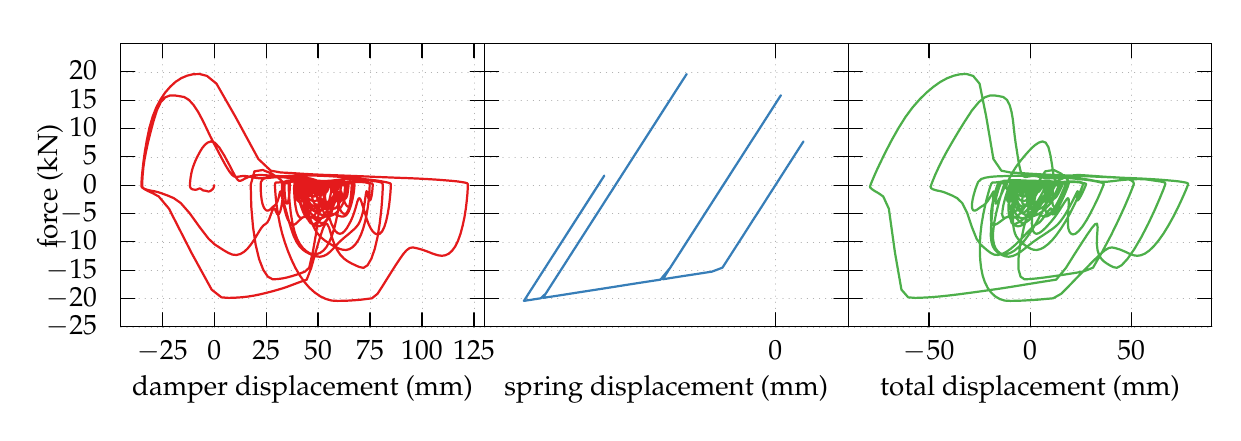
\begin{tikzpicture}[gnuplot]
%% generated with GNUPLOT 5.2p7 (Lua 5.3; terminal rev. Nov 2018, script rev. 107)
%% 08/28/2020 18:28:39
\path (0.000,0.000) rectangle (14.000,4.000);
\gpcolor{color=gp lt color axes}
\gpsetlinetype{gp lt axes}
\gpsetdashtype{gp dt axes}
\gpsetlinewidth{0.50}
\draw[gp path] (0.140,0.200)--(4.759,0.200);
\gpcolor{color=gp lt color border}
\gpsetlinetype{gp lt border}
\gpsetdashtype{gp dt solid}
\gpsetlinewidth{1.00}
\draw[gp path] (0.140,0.200)--(0.320,0.200);
\draw[gp path] (4.759,0.200)--(4.579,0.200);
\node[gp node right] at (-0.044,0.200) {$-25$};
\gpcolor{color=gp lt color axes}
\gpsetlinetype{gp lt axes}
\gpsetdashtype{gp dt axes}
\gpsetlinewidth{0.50}
\draw[gp path] (0.140,0.560)--(4.759,0.560);
\gpcolor{color=gp lt color border}
\gpsetlinetype{gp lt border}
\gpsetdashtype{gp dt solid}
\gpsetlinewidth{1.00}
\draw[gp path] (0.140,0.560)--(0.320,0.560);
\draw[gp path] (4.759,0.560)--(4.579,0.560);
\node[gp node right] at (-0.044,0.560) {$-20$};
\gpcolor{color=gp lt color axes}
\gpsetlinetype{gp lt axes}
\gpsetdashtype{gp dt axes}
\gpsetlinewidth{0.50}
\draw[gp path] (0.140,0.920)--(4.759,0.920);
\gpcolor{color=gp lt color border}
\gpsetlinetype{gp lt border}
\gpsetdashtype{gp dt solid}
\gpsetlinewidth{1.00}
\draw[gp path] (0.140,0.920)--(0.320,0.920);
\draw[gp path] (4.759,0.920)--(4.579,0.920);
\node[gp node right] at (-0.044,0.920) {$-15$};
\gpcolor{color=gp lt color axes}
\gpsetlinetype{gp lt axes}
\gpsetdashtype{gp dt axes}
\gpsetlinewidth{0.50}
\draw[gp path] (0.140,1.280)--(4.759,1.280);
\gpcolor{color=gp lt color border}
\gpsetlinetype{gp lt border}
\gpsetdashtype{gp dt solid}
\gpsetlinewidth{1.00}
\draw[gp path] (0.140,1.280)--(0.320,1.280);
\draw[gp path] (4.759,1.280)--(4.579,1.280);
\node[gp node right] at (-0.044,1.280) {$-10$};
\gpcolor{color=gp lt color axes}
\gpsetlinetype{gp lt axes}
\gpsetdashtype{gp dt axes}
\gpsetlinewidth{0.50}
\draw[gp path] (0.140,1.640)--(4.759,1.640);
\gpcolor{color=gp lt color border}
\gpsetlinetype{gp lt border}
\gpsetdashtype{gp dt solid}
\gpsetlinewidth{1.00}
\draw[gp path] (0.140,1.640)--(0.320,1.640);
\draw[gp path] (4.759,1.640)--(4.579,1.640);
\node[gp node right] at (-0.044,1.640) {$-5$};
\gpcolor{color=gp lt color axes}
\gpsetlinetype{gp lt axes}
\gpsetdashtype{gp dt axes}
\gpsetlinewidth{0.50}
\draw[gp path] (0.140,2.000)--(4.759,2.000);
\gpcolor{color=gp lt color border}
\gpsetlinetype{gp lt border}
\gpsetdashtype{gp dt solid}
\gpsetlinewidth{1.00}
\draw[gp path] (0.140,2.000)--(0.320,2.000);
\draw[gp path] (4.759,2.000)--(4.579,2.000);
\node[gp node right] at (-0.044,2.000) {$0$};
\gpcolor{color=gp lt color axes}
\gpsetlinetype{gp lt axes}
\gpsetdashtype{gp dt axes}
\gpsetlinewidth{0.50}
\draw[gp path] (0.140,2.359)--(4.759,2.359);
\gpcolor{color=gp lt color border}
\gpsetlinetype{gp lt border}
\gpsetdashtype{gp dt solid}
\gpsetlinewidth{1.00}
\draw[gp path] (0.140,2.359)--(0.320,2.359);
\draw[gp path] (4.759,2.359)--(4.579,2.359);
\node[gp node right] at (-0.044,2.359) {$5$};
\gpcolor{color=gp lt color axes}
\gpsetlinetype{gp lt axes}
\gpsetdashtype{gp dt axes}
\gpsetlinewidth{0.50}
\draw[gp path] (0.140,2.719)--(4.759,2.719);
\gpcolor{color=gp lt color border}
\gpsetlinetype{gp lt border}
\gpsetdashtype{gp dt solid}
\gpsetlinewidth{1.00}
\draw[gp path] (0.140,2.719)--(0.320,2.719);
\draw[gp path] (4.759,2.719)--(4.579,2.719);
\node[gp node right] at (-0.044,2.719) {$10$};
\gpcolor{color=gp lt color axes}
\gpsetlinetype{gp lt axes}
\gpsetdashtype{gp dt axes}
\gpsetlinewidth{0.50}
\draw[gp path] (0.140,3.079)--(4.759,3.079);
\gpcolor{color=gp lt color border}
\gpsetlinetype{gp lt border}
\gpsetdashtype{gp dt solid}
\gpsetlinewidth{1.00}
\draw[gp path] (0.140,3.079)--(0.320,3.079);
\draw[gp path] (4.759,3.079)--(4.579,3.079);
\node[gp node right] at (-0.044,3.079) {$15$};
\gpcolor{color=gp lt color axes}
\gpsetlinetype{gp lt axes}
\gpsetdashtype{gp dt axes}
\gpsetlinewidth{0.50}
\draw[gp path] (0.140,3.439)--(4.759,3.439);
\gpcolor{color=gp lt color border}
\gpsetlinetype{gp lt border}
\gpsetdashtype{gp dt solid}
\gpsetlinewidth{1.00}
\draw[gp path] (0.140,3.439)--(0.320,3.439);
\draw[gp path] (4.759,3.439)--(4.579,3.439);
\node[gp node right] at (-0.044,3.439) {$20$};
\gpcolor{color=gp lt color axes}
\gpsetlinetype{gp lt axes}
\gpsetdashtype{gp dt axes}
\gpsetlinewidth{0.50}
\draw[gp path] (0.668,0.200)--(0.668,0.380)--(0.668,3.799);
\gpcolor{color=gp lt color border}
\gpsetlinetype{gp lt border}
\gpsetdashtype{gp dt solid}
\gpsetlinewidth{1.00}
\draw[gp path] (0.668,0.200)--(0.668,0.380);
\draw[gp path] (0.668,3.799)--(0.668,3.619);
\node[gp node center] at (0.668,-0.108) {$-25$};
\gpcolor{color=gp lt color axes}
\gpsetlinetype{gp lt axes}
\gpsetdashtype{gp dt axes}
\gpsetlinewidth{0.50}
\draw[gp path] (1.328,0.200)--(1.328,3.799);
\gpcolor{color=gp lt color border}
\gpsetlinetype{gp lt border}
\gpsetdashtype{gp dt solid}
\gpsetlinewidth{1.00}
\draw[gp path] (1.328,0.200)--(1.328,0.380);
\draw[gp path] (1.328,3.799)--(1.328,3.619);
\node[gp node center] at (1.328,-0.108) {$0$};
\gpcolor{color=gp lt color axes}
\gpsetlinetype{gp lt axes}
\gpsetdashtype{gp dt axes}
\gpsetlinewidth{0.50}
\draw[gp path] (1.988,0.200)--(1.988,3.799);
\gpcolor{color=gp lt color border}
\gpsetlinetype{gp lt border}
\gpsetdashtype{gp dt solid}
\gpsetlinewidth{1.00}
\draw[gp path] (1.988,0.200)--(1.988,0.380);
\draw[gp path] (1.988,3.799)--(1.988,3.619);
\node[gp node center] at (1.988,-0.108) {$25$};
\gpcolor{color=gp lt color axes}
\gpsetlinetype{gp lt axes}
\gpsetdashtype{gp dt axes}
\gpsetlinewidth{0.50}
\draw[gp path] (2.647,0.200)--(2.647,3.799);
\gpcolor{color=gp lt color border}
\gpsetlinetype{gp lt border}
\gpsetdashtype{gp dt solid}
\gpsetlinewidth{1.00}
\draw[gp path] (2.647,0.200)--(2.647,0.380);
\draw[gp path] (2.647,3.799)--(2.647,3.619);
\node[gp node center] at (2.647,-0.108) {$50$};
\gpcolor{color=gp lt color axes}
\gpsetlinetype{gp lt axes}
\gpsetdashtype{gp dt axes}
\gpsetlinewidth{0.50}
\draw[gp path] (3.307,0.200)--(3.307,3.799);
\gpcolor{color=gp lt color border}
\gpsetlinetype{gp lt border}
\gpsetdashtype{gp dt solid}
\gpsetlinewidth{1.00}
\draw[gp path] (3.307,0.200)--(3.307,0.380);
\draw[gp path] (3.307,3.799)--(3.307,3.619);
\node[gp node center] at (3.307,-0.108) {$75$};
\gpcolor{color=gp lt color axes}
\gpsetlinetype{gp lt axes}
\gpsetdashtype{gp dt axes}
\gpsetlinewidth{0.50}
\draw[gp path] (3.967,0.200)--(3.967,3.799);
\gpcolor{color=gp lt color border}
\gpsetlinetype{gp lt border}
\gpsetdashtype{gp dt solid}
\gpsetlinewidth{1.00}
\draw[gp path] (3.967,0.200)--(3.967,0.380);
\draw[gp path] (3.967,3.799)--(3.967,3.619);
\node[gp node center] at (3.967,-0.108) {$100$};
\gpcolor{color=gp lt color axes}
\gpsetlinetype{gp lt axes}
\gpsetdashtype{gp dt axes}
\gpsetlinewidth{0.50}
\draw[gp path] (4.627,0.200)--(4.627,3.799);
\gpcolor{color=gp lt color border}
\gpsetlinetype{gp lt border}
\gpsetdashtype{gp dt solid}
\gpsetlinewidth{1.00}
\draw[gp path] (4.627,0.200)--(4.627,0.380);
\draw[gp path] (4.627,3.799)--(4.627,3.619);
\node[gp node center] at (4.627,-0.108) {$125$};
\draw[gp path] (0.140,3.799)--(0.140,0.200)--(4.759,0.200)--(4.759,3.799)--cycle;
\node[gp node center,rotate=-270] at (-0.750,1.999) {force (\si{\kilo\newton})};
\node[gp node center] at (2.449,-0.569) {damper displacement (\si{\milli\meter})};
\gpcolor{rgb color={0.894,0.102,0.110}}
\gpsetlinewidth{2.00}
\draw[gp path] (1.328,2.000)--(1.328,1.999)--(1.328,1.997)--(1.327,1.993)--(1.326,1.989)%
  --(1.325,1.983)--(1.323,1.977)--(1.321,1.970)--(1.318,1.963)--(1.314,1.956)--(1.310,1.951)%
  --(1.305,1.946)--(1.299,1.941)--(1.293,1.936)--(1.286,1.931)--(1.278,1.926)--(1.270,1.922)%
  --(1.260,1.920)--(1.251,1.920)--(1.240,1.923)--(1.230,1.926)--(1.220,1.929)--(1.210,1.930)%
  --(1.200,1.931)--(1.189,1.933)--(1.179,1.938)--(1.169,1.946)--(1.161,1.952)--(1.153,1.956)%
  --(1.146,1.957)--(1.139,1.957)--(1.131,1.954)--(1.123,1.950)--(1.113,1.946)--(1.102,1.943)%
  --(1.090,1.942)--(1.077,1.943)--(1.064,1.944)--(1.052,1.948)--(1.041,1.953)--(1.031,1.961)%
  --(1.025,1.972)--(1.021,1.984)--(1.020,2.000)--(1.021,2.025)--(1.024,2.059)--(1.029,2.099)%
  --(1.036,2.141)--(1.045,2.183)--(1.057,2.224)--(1.071,2.263)--(1.087,2.303)--(1.105,2.343)%
  --(1.127,2.386)--(1.151,2.430)--(1.178,2.474)--(1.210,2.512)--(1.245,2.541)--(1.286,2.555)%
  --(1.334,2.540)--(1.391,2.481)--(1.457,2.375)--(1.522,2.254)--(1.572,2.157)--(1.605,2.097)%
  --(1.627,2.067)--(1.643,2.056)--(1.658,2.054)--(1.674,2.060)--(1.694,2.070)--(1.719,2.083)%
  --(1.753,2.099)--(1.797,2.115)--(1.852,2.126)--(1.918,2.129)--(1.990,2.125)--(2.066,2.120)%
  --(2.145,2.115)--(2.226,2.109)--(2.309,2.104)--(2.392,2.100)--(2.477,2.095)--(2.557,2.083)%
  --(2.622,2.063)--(2.662,2.040)--(2.677,2.017)--(2.678,1.966)--(2.673,1.867)--(2.663,1.727)%
  --(2.645,1.557)--(2.618,1.364)--(2.582,1.159)--(2.535,0.952)--(2.481,0.902)--(2.425,0.881)%
  --(2.368,0.861)--(2.310,0.843)--(2.251,0.827)--(2.191,0.815)--(2.131,0.807)--(2.070,0.805)%
  --(2.009,0.838)--(1.951,0.925)--(1.898,1.062)--(1.854,1.246)--(1.821,1.470)--(1.799,1.727)%
  --(1.792,2.005)--(1.839,2.175)--(1.945,2.193)--(2.055,2.148)--(2.137,2.096)--(2.185,2.056)%
  --(2.204,2.022)--(2.205,1.978)--(2.202,1.905)--(2.195,1.820)--(2.183,1.736)--(2.168,1.670)%
  --(2.150,1.631)--(2.131,1.628)--(2.113,1.662)--(2.096,1.702)--(2.081,1.703)--(2.065,1.674)%
  --(2.047,1.625)--(2.027,1.571)--(2.004,1.528)--(1.979,1.506)--(1.953,1.488)--(1.926,1.456)%
  --(1.897,1.410)--(1.865,1.356)--(1.830,1.298)--(1.791,1.242)--(1.750,1.192)--(1.706,1.152)%
  --(1.659,1.125)--(1.610,1.113)--(1.560,1.118)--(1.509,1.139)--(1.456,1.169)--(1.401,1.204)%
  --(1.338,1.245)--(1.258,1.318)--(1.147,1.462)--(1.016,1.644)--(0.903,1.773)--(0.813,1.836)%
  --(0.737,1.868)--(0.671,1.892)--(0.615,1.911)--(0.567,1.923)--(0.524,1.930)--(0.485,1.939)%
  --(0.453,1.949)--(0.430,1.961)--(0.416,1.975)--(0.413,1.998)--(0.415,2.051)--(0.420,2.134)%
  --(0.429,2.227)--(0.443,2.325)--(0.463,2.429)--(0.487,2.542)--(0.518,2.667)--(0.555,2.806)%
  --(0.600,2.950)--(0.651,3.057)--(0.708,3.116)--(0.767,3.139)--(0.827,3.139)--(0.887,3.130)%
  --(0.947,3.119)--(1.007,3.083)--(1.066,3.018)--(1.123,2.932)--(1.176,2.833)--(1.227,2.729)%
  --(1.275,2.627)--(1.324,2.531)--(1.374,2.436)--(1.426,2.337)--(1.476,2.246)--(1.519,2.176)%
  --(1.554,2.131)--(1.584,2.109)--(1.613,2.104)--(1.644,2.109)--(1.680,2.115)--(1.722,2.116)%
  --(1.766,2.110)--(1.810,2.100)--(1.853,2.093)--(1.895,2.088)--(1.939,2.087)--(1.985,2.089)%
  --(2.037,2.094)--(2.097,2.100)--(2.166,2.103)--(2.238,2.097)--(2.307,2.087)--(2.371,2.079)%
  --(2.430,2.072)--(2.483,2.063)--(2.529,2.055)--(2.568,2.050)--(2.602,2.045)--(2.633,2.043)%
  --(2.663,2.042)--(2.693,2.043)--(2.727,2.047)--(2.766,2.051)--(2.814,2.057)--(2.871,2.064)%
  --(2.938,2.070)--(3.016,2.075)--(3.102,2.077)--(3.192,2.073)--(3.271,2.063)--(3.337,2.054)%
  --(3.391,2.047)--(3.434,2.039)--(3.461,2.028)--(3.469,2.009)--(3.468,1.945)--(3.462,1.831)%
  --(3.450,1.681)--(3.430,1.513)--(3.403,1.344)--(3.367,1.190)--(3.324,1.066)--(3.276,0.983)%
  --(3.225,0.950)--(3.172,0.960)--(3.122,0.982)--(3.072,1.006)--(3.023,1.033)--(2.976,1.068)%
  --(2.931,1.114)--(2.889,1.176)--(2.851,1.258)--(2.816,1.362)--(2.787,1.461)--(2.761,1.510)%
  --(2.737,1.504)--(2.711,1.453)--(2.682,1.368)--(2.648,1.258)--(2.608,1.120)--(2.560,0.949)%
  --(2.503,0.800)--(2.442,0.779)--(2.380,0.756)--(2.316,0.732)--(2.252,0.708)--(2.185,0.686)%
  --(2.117,0.666)--(2.048,0.647)--(1.977,0.629)--(1.905,0.612)--(1.831,0.597)--(1.756,0.585)%
  --(1.678,0.576)--(1.598,0.571)--(1.514,0.568)--(1.420,0.575)--(1.296,0.673)--(1.039,1.142)%
  --(0.754,1.701)--(0.624,1.856)--(0.547,1.898)--(0.490,1.924)--(0.450,1.945)--(0.425,1.961)%
  --(0.411,1.972)--(0.405,1.982)--(0.404,2.002)--(0.405,2.040)--(0.409,2.100)--(0.417,2.184)%
  --(0.429,2.292)--(0.447,2.423)--(0.473,2.573)--(0.505,2.727)--(0.546,2.868)--(0.593,2.988)%
  --(0.647,3.088)--(0.705,3.175)--(0.769,3.249)--(0.836,3.311)--(0.908,3.358)--(0.983,3.390)%
  --(1.062,3.409)--(1.145,3.411)--(1.237,3.387)--(1.357,3.289)--(1.598,2.868)--(1.889,2.332)%
  --(2.047,2.184)--(2.172,2.161)--(2.302,2.154)--(2.440,2.145)--(2.583,2.137)--(2.731,2.130)%
  --(2.883,2.125)--(3.039,2.119)--(3.196,2.113)--(3.351,2.106)--(3.503,2.100)--(3.650,2.094)%
  --(3.792,2.089)--(3.928,2.083)--(4.055,2.076)--(4.168,2.069)--(4.267,2.061)--(4.351,2.054)%
  --(4.420,2.047)--(4.474,2.039)--(4.514,2.032)--(4.538,2.025)--(4.548,2.017)--(4.549,1.998)%
  --(4.548,1.956)--(4.544,1.891)--(4.536,1.806)--(4.524,1.704)--(4.507,1.596)--(4.484,1.488)%
  --(4.457,1.385)--(4.425,1.295)--(4.389,1.221)--(4.349,1.167)--(4.308,1.130)--(4.265,1.110)%
  --(4.221,1.103)--(4.177,1.108)--(4.134,1.120)--(4.091,1.135)--(4.049,1.152)--(4.008,1.167)%
  --(3.968,1.181)--(3.928,1.192)--(3.889,1.202)--(3.850,1.209)--(3.811,1.202)--(3.771,1.173)%
  --(3.729,1.125)--(3.685,1.062)--(3.637,0.990)--(3.586,0.910)--(3.530,0.821)--(3.469,0.723)%
  --(3.403,0.621)--(3.332,0.563)--(3.261,0.554)--(3.188,0.545)--(3.115,0.539)--(3.042,0.534)%
  --(2.968,0.531)--(2.895,0.530)--(2.821,0.534)--(2.748,0.554)--(2.676,0.588)--(2.606,0.636)%
  --(2.538,0.696)--(2.475,0.769)--(2.415,0.854)--(2.359,0.950)--(2.309,1.055)--(2.264,1.164)%
  --(2.225,1.274)--(2.191,1.386)--(2.163,1.501)--(2.141,1.617)--(2.124,1.725)--(2.112,1.822)%
  --(2.105,1.903)--(2.101,1.968)--(2.101,2.017)--(2.110,2.034)--(2.124,2.034)--(2.138,2.034)%
  --(2.153,2.035)--(2.169,2.037)--(2.188,2.039)--(2.208,2.042)--(2.232,2.047)--(2.261,2.053)%
  --(2.296,2.057)--(2.335,2.061)--(2.378,2.062)--(2.423,2.062)--(2.469,2.061)--(2.515,2.059)%
  --(2.560,2.057)--(2.604,2.055)--(2.648,2.053)--(2.690,2.052)--(2.732,2.052)--(2.777,2.053)%
  --(2.822,2.051)--(2.864,2.047)--(2.901,2.043)--(2.934,2.040)--(2.962,2.036)--(2.986,2.032)%
  --(3.005,2.028)--(3.018,2.025)--(3.027,2.020)--(3.031,2.014)--(3.032,2.000)--(3.031,1.978)%
  --(3.029,1.947)--(3.025,1.914)--(3.020,1.883)--(3.013,1.858)--(3.005,1.841)--(2.996,1.831)%
  --(2.988,1.829)--(2.979,1.835)--(2.971,1.845)--(2.963,1.860)--(2.956,1.875)--(2.949,1.892)%
  --(2.944,1.909)--(2.939,1.925)--(2.935,1.921)--(2.930,1.889)--(2.923,1.830)--(2.912,1.750)%
  --(2.897,1.656)--(2.878,1.555)--(2.853,1.454)--(2.824,1.360)--(2.790,1.279)--(2.753,1.213)%
  --(2.713,1.167)--(2.670,1.138)--(2.627,1.124)--(2.584,1.122)--(2.540,1.135)--(2.498,1.162)%
  --(2.457,1.199)--(2.418,1.249)--(2.382,1.315)--(2.350,1.402)--(2.323,1.511)--(2.301,1.645)%
  --(2.286,1.781)--(2.278,1.888)--(2.274,1.966)--(2.274,2.017)--(2.282,2.028)--(2.289,2.017)%
  --(2.290,1.996)--(2.288,1.960)--(2.285,1.910)--(2.278,1.852)--(2.269,1.801)--(2.258,1.768)%
  --(2.246,1.767)--(2.235,1.804)--(2.226,1.866)--(2.221,1.940)--(2.220,2.022)--(2.243,2.054)%
  --(2.278,2.057)--(2.314,2.054)--(2.346,2.048)--(2.373,2.040)--(2.393,2.033)--(2.407,2.029)%
  --(2.419,2.028)--(2.432,2.031)--(2.450,2.038)--(2.478,2.049)--(2.517,2.058)--(2.562,2.057)%
  --(2.606,2.055)--(2.649,2.053)--(2.692,2.052)--(2.734,2.051)--(2.777,2.053)--(2.823,2.053)%
  --(2.868,2.049)--(2.906,2.043)--(2.938,2.039)--(2.966,2.036)--(2.991,2.034)--(3.013,2.032)%
  --(3.034,2.033)--(3.058,2.035)--(3.085,2.037)--(3.116,2.040)--(3.149,2.040)--(3.184,2.040)%
  --(3.216,2.038)--(3.246,2.035)--(3.270,2.030)--(3.287,2.026)--(3.300,2.024)--(3.310,2.023)%
  --(3.320,2.023)--(3.329,2.021)--(3.335,2.019)--(3.339,2.015)--(3.341,2.007)--(3.341,1.990)%
  --(3.339,1.963)--(3.336,1.928)--(3.331,1.888)--(3.324,1.850)--(3.316,1.820)--(3.306,1.804)%
  --(3.296,1.808)--(3.287,1.833)--(3.279,1.868)--(3.273,1.901)--(3.268,1.919)--(3.263,1.923)%
  --(3.259,1.912)--(3.253,1.878)--(3.245,1.821)--(3.235,1.750)--(3.220,1.675)--(3.202,1.605)%
  --(3.181,1.546)--(3.158,1.501)--(3.132,1.468)--(3.105,1.440)--(3.077,1.416)--(3.048,1.390)%
  --(3.017,1.364)--(2.985,1.338)--(2.952,1.309)--(2.917,1.277)--(2.880,1.239)--(2.842,1.196)%
  --(2.801,1.154)--(2.758,1.120)--(2.714,1.099)--(2.669,1.091)--(2.624,1.096)--(2.579,1.110)%
  --(2.535,1.130)--(2.492,1.153)--(2.451,1.183)--(2.411,1.224)--(2.374,1.279)--(2.339,1.351)%
  --(2.309,1.436)--(2.282,1.524)--(2.260,1.605)--(2.242,1.671)--(2.227,1.723)--(2.214,1.764)%
  --(2.202,1.799)--(2.193,1.831)--(2.184,1.864)--(2.178,1.894)--(2.172,1.914)--(2.168,1.920)%
  --(2.163,1.910)--(2.157,1.888)--(2.151,1.857)--(2.142,1.824)--(2.132,1.794)--(2.121,1.770)%
  --(2.108,1.753)--(2.095,1.741)--(2.081,1.731)--(2.067,1.719)--(2.052,1.704)--(2.037,1.690)%
  --(2.020,1.679)--(2.004,1.676)--(1.987,1.682)--(1.971,1.697)--(1.956,1.723)--(1.942,1.761)%
  --(1.931,1.812)--(1.923,1.877)--(1.918,1.956)--(1.921,2.039)--(1.949,2.079)--(1.996,2.095)%
  --(2.055,2.105)--(2.125,2.111)--(2.205,2.114)--(2.295,2.117)--(2.395,2.119)--(2.507,2.121)%
  --(2.630,2.121)--(2.760,2.116)--(2.890,2.108)--(3.014,2.097)--(3.126,2.087)--(3.227,2.077)%
  --(3.316,2.068)--(3.392,2.059)--(3.452,2.049)--(3.498,2.040)--(3.530,2.033)--(3.552,2.027)%
  --(3.565,2.022)--(3.571,2.014)--(3.572,1.996)--(3.570,1.960)--(3.566,1.903)--(3.559,1.828)%
  --(3.549,1.739)--(3.533,1.642)--(3.513,1.548)--(3.489,1.471)--(3.462,1.415)--(3.432,1.382)%
  --(3.402,1.374)--(3.371,1.386)--(3.342,1.412)--(3.314,1.454)--(3.288,1.509)--(3.265,1.571)%
  --(3.246,1.633)--(3.229,1.688)--(3.214,1.735)--(3.202,1.775)--(3.191,1.806)--(3.182,1.825)%
  --(3.173,1.834)--(3.165,1.832)--(3.155,1.815)--(3.145,1.787)--(3.134,1.746)--(3.120,1.697)%
  --(3.103,1.644)--(3.084,1.593)--(3.063,1.545)--(3.039,1.500)--(3.014,1.456)--(2.986,1.419)%
  --(2.957,1.392)--(2.926,1.382)--(2.896,1.391)--(2.866,1.418)--(2.839,1.463)--(2.813,1.520)%
  --(2.791,1.587)--(2.772,1.656)--(2.757,1.724)--(2.744,1.790)--(2.735,1.856)--(2.729,1.920)%
  --(2.726,1.983)--(2.731,2.031)--(2.754,2.038)--(2.783,2.041)--(2.814,2.043)--(2.846,2.041)%
  --(2.876,2.038)--(2.901,2.034)--(2.920,2.028)--(2.932,2.023)--(2.938,2.017)--(2.940,2.008)%
  --(2.941,1.993)--(2.940,1.979)--(2.938,1.970)--(2.936,1.958)--(2.933,1.941)--(2.929,1.924)%
  --(2.924,1.913)--(2.919,1.912)--(2.914,1.912)--(2.909,1.901)--(2.903,1.878)--(2.896,1.853)%
  --(2.888,1.832)--(2.879,1.816)--(2.869,1.804)--(2.859,1.791)--(2.848,1.776)--(2.836,1.760)%
  --(2.823,1.742)--(2.810,1.725)--(2.796,1.710)--(2.781,1.698)--(2.765,1.692)--(2.750,1.693)%
  --(2.735,1.705)--(2.721,1.732)--(2.708,1.772)--(2.697,1.810)--(2.688,1.831)--(2.679,1.829)%
  --(2.670,1.806)--(2.659,1.768)--(2.646,1.723)--(2.631,1.677)--(2.614,1.637)--(2.595,1.607)%
  --(2.575,1.590)--(2.554,1.590)--(2.534,1.595)--(2.513,1.599)--(2.493,1.601)--(2.473,1.597)%
  --(2.453,1.590)--(2.432,1.585)--(2.412,1.592)--(2.392,1.618)--(2.374,1.668)--(2.359,1.745)%
  --(2.348,1.845)--(2.342,1.961)--(2.352,2.052)--(2.393,2.062)--(2.437,2.058)--(2.478,2.054)%
  --(2.516,2.052)--(2.553,2.050)--(2.591,2.051)--(2.629,2.050)--(2.666,2.047)--(2.701,2.044)%
  --(2.731,2.041)--(2.759,2.039)--(2.785,2.037)--(2.809,2.035)--(2.830,2.032)--(2.848,2.029)%
  --(2.862,2.025)--(2.871,2.020)--(2.875,2.016)--(2.877,2.011)--(2.878,2.008)--(2.879,2.007)%
  --(2.880,2.010)--(2.882,2.016)--(2.887,2.021)--(2.894,2.023)--(2.903,2.022)--(2.909,2.018)%
  --(2.912,2.009)--(2.912,1.997)--(2.912,1.984)--(2.910,1.975)--(2.908,1.973)--(2.907,1.972)%
  --(2.905,1.968)--(2.902,1.959)--(2.900,1.947)--(2.896,1.940)--(2.893,1.941)--(2.890,1.953)%
  --(2.887,1.974)--(2.886,1.994)--(2.886,2.006)--(2.887,2.007)--(2.887,1.998)--(2.887,1.982)%
  --(2.885,1.963)--(2.882,1.943)--(2.878,1.926)--(2.874,1.908)--(2.868,1.885)--(2.861,1.855)%
  --(2.853,1.821)--(2.843,1.787)--(2.831,1.759)--(2.818,1.738)--(2.805,1.723)--(2.791,1.713)%
  --(2.776,1.712)--(2.762,1.723)--(2.748,1.747)--(2.736,1.782)--(2.726,1.822)--(2.718,1.866)%
  --(2.712,1.913)--(2.708,1.966)--(2.708,2.017)--(2.722,2.032)--(2.738,2.028)--(2.749,2.022)%
  --(2.753,2.013)--(2.754,1.998)--(2.753,1.978)--(2.751,1.956)--(2.748,1.936)--(2.744,1.914)%
  --(2.738,1.886)--(2.731,1.853)--(2.723,1.819)--(2.713,1.788)--(2.701,1.764)--(2.689,1.751)%
  --(2.676,1.747)--(2.663,1.747)--(2.650,1.751)--(2.638,1.753)--(2.625,1.754)--(2.613,1.758)%
  --(2.601,1.767)--(2.589,1.786)--(2.579,1.816)--(2.570,1.857)--(2.564,1.905)--(2.560,1.953)%
  --(2.558,1.991)--(2.558,2.006)--(2.559,2.003)--(2.559,1.989)--(2.557,1.971)--(2.555,1.955)%
  --(2.552,1.945)--(2.549,1.942)--(2.545,1.943)--(2.542,1.950)--(2.539,1.962)--(2.537,1.979)%
  --(2.537,1.998)--(2.538,2.016)--(2.544,2.024)--(2.553,2.025)--(2.562,2.024)--(2.569,2.021)%
  --(2.574,2.018)--(2.578,2.016)--(2.581,2.017)--(2.584,2.018)--(2.589,2.018)--(2.592,2.016)%
  --(2.594,2.012)--(2.596,2.005)--(2.596,1.996)--(2.595,1.986)--(2.594,1.975)--(2.592,1.965)%
  --(2.589,1.957)--(2.586,1.950)--(2.583,1.944)--(2.580,1.938)--(2.576,1.937)--(2.573,1.946)%
  --(2.570,1.970)--(2.569,2.009)--(2.581,2.035)--(2.605,2.041)--(2.634,2.043)--(2.664,2.043)%
  --(2.694,2.041)--(2.721,2.038)--(2.744,2.035)--(2.765,2.033)--(2.784,2.031)--(2.802,2.030)%
  --(2.819,2.030)--(2.834,2.028)--(2.847,2.025)--(2.856,2.021)--(2.860,2.014)--(2.861,1.997)%
  --(2.860,1.971)--(2.857,1.937)--(2.853,1.902)--(2.847,1.868)--(2.839,1.840)--(2.830,1.814)%
  --(2.820,1.788)--(2.808,1.761)--(2.795,1.733)--(2.781,1.706)--(2.766,1.682)--(2.749,1.657)%
  --(2.732,1.632)--(2.713,1.606)--(2.692,1.580)--(2.671,1.557)--(2.648,1.537)--(2.625,1.520)%
  --(2.601,1.509)--(2.576,1.506)--(2.552,1.518)--(2.528,1.550)--(2.507,1.600)--(2.489,1.664)%
  --(2.473,1.738)--(2.462,1.814)--(2.454,1.883)--(2.449,1.941)--(2.447,1.987)--(2.448,2.018)%
  --(2.456,2.026)--(2.466,2.025)--(2.475,2.024)--(2.483,2.024)--(2.492,2.023)--(2.499,2.022)%
  --(2.505,2.020)--(2.510,2.019)--(2.514,2.019)--(2.519,2.020)--(2.525,2.022)--(2.532,2.023)%
  --(2.540,2.023)--(2.548,2.023)--(2.556,2.025)--(2.567,2.028)--(2.581,2.030)--(2.595,2.030)%
  --(2.610,2.029)--(2.623,2.028)--(2.636,2.028)--(2.650,2.028)--(2.664,2.029)--(2.678,2.029)%
  --(2.692,2.029)--(2.707,2.029)--(2.722,2.029)--(2.736,2.029)--(2.751,2.029)--(2.767,2.029)%
  --(2.783,2.030)--(2.800,2.030)--(2.817,2.031)--(2.836,2.032)--(2.857,2.033)--(2.879,2.034)%
  --(2.901,2.033)--(2.921,2.032)--(2.940,2.029)--(2.955,2.027)--(2.968,2.026)--(2.979,2.023)%
  --(2.987,2.019)--(2.990,2.010)--(2.990,1.990)--(2.988,1.958)--(2.985,1.920)--(2.980,1.883)%
  --(2.973,1.856)--(2.965,1.837)--(2.956,1.822)--(2.946,1.810)--(2.936,1.799)--(2.926,1.786)%
  --(2.914,1.769)--(2.902,1.748)--(2.889,1.727)--(2.875,1.712)--(2.860,1.703)--(2.845,1.701)%
  --(2.830,1.706)--(2.816,1.716)--(2.802,1.733)--(2.789,1.754)--(2.777,1.775)--(2.765,1.788)%
  --(2.755,1.791)--(2.744,1.785)--(2.732,1.770)--(2.720,1.748)--(2.707,1.721)--(2.692,1.692)%
  --(2.676,1.666)--(2.659,1.648)--(2.641,1.643)--(2.623,1.650)--(2.606,1.667)--(2.590,1.688)%
  --(2.575,1.710)--(2.560,1.730)--(2.547,1.745)--(2.534,1.757)--(2.522,1.767)--(2.511,1.782)%
  --(2.500,1.806)--(2.491,1.840)--(2.483,1.881)--(2.478,1.921)--(2.474,1.957)--(2.472,1.985)%
  --(2.472,2.002)--(2.473,2.008)--(2.474,2.004)--(2.474,1.993)--(2.472,1.975)--(2.470,1.951)%
  --(2.467,1.922)--(2.461,1.890)--(2.455,1.858)--(2.446,1.828)--(2.437,1.805)--(2.426,1.790)%
  --(2.415,1.785)--(2.404,1.789)--(2.394,1.798)--(2.383,1.812)--(2.374,1.829)--(2.366,1.853)%
  --(2.359,1.888)--(2.354,1.937)--(2.352,1.998)--(2.363,2.042)--(2.393,2.052)--(2.430,2.056)%
  --(2.472,2.057)--(2.514,2.057)--(2.556,2.053)--(2.595,2.049)--(2.628,2.043)--(2.655,2.037)%
  --(2.676,2.032)--(2.691,2.027)--(2.703,2.024)--(2.711,2.023)--(2.720,2.024)--(2.731,2.027)%
  --(2.745,2.030)--(2.764,2.033)--(2.785,2.034)--(2.807,2.035)--(2.829,2.034)--(2.850,2.031)%
  --(2.867,2.029)--(2.882,2.027)--(2.896,2.027)--(2.911,2.029)--(2.928,2.031)--(2.949,2.034)%
  --(2.973,2.036)--(3.000,2.036)--(3.026,2.035)--(3.050,2.033)--(3.070,2.029)--(3.083,2.023)%
  --(3.089,2.014)--(3.090,1.992)--(3.088,1.951)--(3.084,1.898)--(3.077,1.840)--(3.067,1.790)%
  --(3.056,1.752)--(3.043,1.731)--(3.029,1.727)--(3.015,1.734)--(3.002,1.750)--(2.990,1.772)%
  --(2.979,1.796)--(2.969,1.817)--(2.960,1.831)--(2.952,1.838)--(2.943,1.841)--(2.935,1.842)%
  --(2.927,1.846)--(2.919,1.854)--(2.912,1.868)--(2.905,1.886)--(2.899,1.903)--(2.894,1.916)%
  --(2.890,1.921)--(2.885,1.917)--(2.880,1.902)--(2.874,1.876)--(2.867,1.840)--(2.858,1.797)%
  --(2.846,1.747)--(2.832,1.697)--(2.816,1.650)--(2.797,1.609)--(2.777,1.574)--(2.755,1.547)%
  --(2.732,1.529)--(2.708,1.520)--(2.685,1.520)--(2.661,1.529)--(2.638,1.544)--(2.615,1.561)%
  --(2.594,1.578)--(2.573,1.591)--(2.553,1.599)--(2.533,1.604)--(2.513,1.606)--(2.493,1.605)%
  --(2.473,1.600)--(2.453,1.590)--(2.432,1.575)--(2.410,1.554)--(2.387,1.531)--(2.363,1.509)%
  --(2.339,1.497)--(2.313,1.500)--(2.289,1.520)--(2.265,1.559)--(2.244,1.612)--(2.226,1.675)%
  --(2.211,1.745)--(2.200,1.817)--(2.192,1.890)--(2.188,1.961)--(2.188,2.019)--(2.201,2.037)%
  --(2.217,2.033)--(2.229,2.028)--(2.238,2.025)--(2.246,2.024)--(2.254,2.026)--(2.265,2.031)%
  --(2.280,2.036)--(2.301,2.041)--(2.325,2.045)--(2.354,2.048)--(2.384,2.049)--(2.417,2.050)%
  --(2.452,2.051)--(2.489,2.053)--(2.528,2.054)--(2.569,2.055)--(2.613,2.055)--(2.657,2.055)%
  --(2.702,2.054)--(2.746,2.053)--(2.790,2.051)--(2.832,2.049)--(2.873,2.047)--(2.911,2.044)%
  --(2.945,2.040)--(2.973,2.035)--(2.995,2.030)--(3.009,2.024)--(3.017,2.020)--(3.022,2.017)%
  --(3.025,2.015)--(3.027,2.015)--(3.031,2.019)--(3.037,2.021)--(3.045,2.022)--(3.053,2.023)%
  --(3.063,2.024)--(3.073,2.024)--(3.083,2.024)--(3.093,2.023)--(3.101,2.021)--(3.106,2.017)%
  --(3.109,2.008)--(3.109,1.993)--(3.108,1.970)--(3.105,1.942)--(3.101,1.909)--(3.095,1.873)%
  --(3.087,1.834)--(3.078,1.792)--(3.066,1.748)--(3.052,1.706)--(3.037,1.667)--(3.019,1.637)%
  --(3.001,1.616)--(2.981,1.605)--(2.961,1.601)--(2.942,1.602)--(2.922,1.607)--(2.903,1.614)%
  --(2.884,1.622)--(2.865,1.629)--(2.847,1.634)--(2.828,1.634)--(2.810,1.626)--(2.791,1.608)%
  --(2.771,1.582)--(2.749,1.552)--(2.726,1.523)--(2.702,1.499)--(2.677,1.483)--(2.651,1.477)%
  --(2.625,1.481)--(2.599,1.494)--(2.575,1.513)--(2.551,1.536)--(2.528,1.558)--(2.507,1.580)%
  --(2.486,1.606)--(2.467,1.640)--(2.450,1.680)--(2.435,1.721)--(2.422,1.760)--(2.410,1.794)%
  --(2.400,1.824)--(2.392,1.852)--(2.385,1.882)--(2.379,1.916)--(2.375,1.955)--(2.374,1.997)%
  --(2.378,2.027)--(2.390,2.030)--(2.402,2.026)--(2.409,2.022)--(2.414,2.019)--(2.418,2.018)%
  --(2.423,2.020)--(2.429,2.024)--(2.438,2.026)--(2.449,2.027)--(2.459,2.026)--(2.469,2.024)%
  --(2.476,2.020)--(2.480,2.014)--(2.481,2.005)--(2.481,1.998)--(2.482,2.012)--(2.489,2.030)%
  --(2.509,2.041)--(2.539,2.048)--(2.575,2.051)--(2.613,2.050)--(2.648,2.045)--(2.677,2.037)%
  --(2.696,2.028)--(2.705,2.020)--(2.709,2.011)--(2.709,2.000)--(2.709,1.993)--(2.709,1.992)%
  --(2.708,1.997)--(2.708,2.004)--(2.709,2.010)--(2.711,2.017)--(2.717,2.022)--(2.726,2.026)%
  --(2.740,2.030)--(2.758,2.033)--(2.780,2.036)--(2.806,2.039)--(2.836,2.042)--(2.870,2.044)%
  --(2.906,2.045)--(2.943,2.043)--(2.977,2.041)--(3.007,2.037)--(3.032,2.033)--(3.051,2.029)%
  --(3.065,2.024)--(3.072,2.018)--(3.074,2.004)--(3.073,1.974)--(3.070,1.927)--(3.065,1.866)%
  --(3.056,1.798)--(3.045,1.735)--(3.030,1.684)--(3.013,1.651)--(2.996,1.636)--(2.977,1.635)%
  --(2.959,1.646)--(2.942,1.665)--(2.926,1.694)--(2.912,1.734)--(2.899,1.783)--(2.890,1.834)%
  --(2.882,1.881)--(2.877,1.920)--(2.873,1.948)--(2.870,1.964)--(2.868,1.965)--(2.865,1.950)%
  --(2.862,1.919)--(2.856,1.874)--(2.848,1.815)--(2.837,1.747)--(2.823,1.683)--(2.806,1.632)%
  --(2.786,1.601)--(2.766,1.593)--(2.746,1.607)--(2.727,1.637)--(2.710,1.679)--(2.695,1.731)%
  --(2.683,1.794)--(2.674,1.867)--(2.669,1.949)--(2.672,2.029)--(2.703,2.050)--(2.745,2.054)%
  --(2.792,2.055)--(2.840,2.053)--(2.883,2.047)--(2.916,2.037)--(2.936,2.027)--(2.944,2.018)%
  --(2.947,2.007)--(2.947,1.996)--(2.947,1.994)--(2.946,2.002)--(2.948,2.015)--(2.952,2.021)%
  --(2.959,2.020)--(2.963,2.015)--(2.964,2.007)--(2.965,1.999)--(2.965,1.996)--(2.965,2.005)%
  --(2.969,2.024)--(2.985,2.032)--(3.010,2.038)--(3.042,2.042)--(3.080,2.045)--(3.122,2.046)%
  --(3.165,2.046)--(3.208,2.044)--(3.246,2.040)--(3.277,2.034)--(3.296,2.025)--(3.302,2.011)%
  --(3.302,1.976)--(3.299,1.912)--(3.292,1.828)--(3.281,1.733)--(3.265,1.635)--(3.245,1.538)%
  --(3.220,1.448)--(3.191,1.368)--(3.158,1.301)--(3.122,1.249)--(3.084,1.211)--(3.045,1.187)%
  --(3.005,1.177)--(2.964,1.179)--(2.924,1.190)--(2.884,1.207)--(2.845,1.227)--(2.808,1.249)%
  --(2.771,1.272)--(2.735,1.296)--(2.701,1.323)--(2.668,1.354)--(2.637,1.392)--(2.608,1.437)%
  --(2.582,1.490)--(2.558,1.547)--(2.536,1.605)--(2.518,1.659)--(2.502,1.707)--(2.488,1.747)%
  --(2.476,1.779)--(2.465,1.804)--(2.455,1.819)--(2.446,1.828)--(2.437,1.835)--(2.429,1.843)%
  --(2.421,1.856)--(2.414,1.874)--(2.408,1.897)--(2.402,1.922)--(2.399,1.947)--(2.396,1.970)%
  --(2.395,1.990)--(2.395,2.007)--(2.397,2.020)--(2.404,2.024)--(2.412,2.025)--(2.422,2.026)%
  --(2.432,2.026)--(2.442,2.026)--(2.452,2.026)--(2.462,2.026)--(2.472,2.026)--(2.483,2.026)%
  --(2.492,2.024)--(2.500,2.022)--(2.506,2.020)--(2.510,2.015)--(2.511,2.007)--(2.512,1.997)%
  --(2.511,1.985)--(2.509,1.975)--(2.508,1.968)--(2.505,1.963)--(2.503,1.959)--(2.500,1.955)%
  --(2.497,1.950)--(2.494,1.944)--(2.491,1.936)--(2.487,1.924)--(2.482,1.908)--(2.476,1.887)%
  --(2.470,1.864)--(2.462,1.841)--(2.453,1.820)--(2.443,1.804)--(2.433,1.796)--(2.423,1.798)%
  --(2.412,1.811)--(2.403,1.836)--(2.395,1.871)--(2.389,1.911)--(2.385,1.951)--(2.383,1.988)%
  --(2.384,2.016)--(2.390,2.024)--(2.398,2.023)--(2.405,2.022)--(2.411,2.021)--(2.417,2.021)%
  --(2.423,2.022)--(2.430,2.024)--(2.439,2.027)--(2.452,2.030)--(2.466,2.032)--(2.483,2.033)%
  --(2.500,2.033)--(2.517,2.031)--(2.532,2.029)--(2.544,2.027)--(2.556,2.027)--(2.568,2.027)%
  --(2.580,2.029)--(2.596,2.031)--(2.613,2.033)--(2.633,2.034)--(2.653,2.035)--(2.674,2.035)%
  --(2.695,2.034)--(2.716,2.034)--(2.736,2.033)--(2.755,2.032)--(2.772,2.030)--(2.788,2.028)%
  --(2.801,2.026)--(2.812,2.025)--(2.822,2.024)--(2.831,2.022)--(2.837,2.020)--(2.841,2.015)%
  --(2.843,2.006)--(2.843,1.991)--(2.841,1.971)--(2.839,1.950)--(2.836,1.930)--(2.831,1.915)%
  --(2.826,1.909)--(2.821,1.912)--(2.817,1.923)--(2.813,1.941)--(2.810,1.963)--(2.808,1.986)%
  --(2.808,2.005)--(2.810,2.017)--(2.814,2.019)--(2.819,2.017)--(2.821,2.013)--(2.823,2.006)%
  --(2.823,1.996)--(2.822,1.982)--(2.820,1.965)--(2.818,1.946)--(2.814,1.922)--(2.809,1.894)%
  --(2.802,1.861)--(2.794,1.825)--(2.784,1.788)--(2.773,1.754)--(2.759,1.727)--(2.745,1.709)%
  --(2.730,1.701)--(2.715,1.703)--(2.700,1.713)--(2.686,1.729)--(2.673,1.749)--(2.661,1.772)%
  --(2.650,1.798)--(2.640,1.826)--(2.632,1.854)--(2.625,1.878)--(2.619,1.898)--(2.613,1.911)%
  --(2.609,1.921)--(2.604,1.928)--(2.600,1.934)--(2.597,1.940)--(2.593,1.944)--(2.590,1.946)%
  --(2.587,1.945)--(2.583,1.942)--(2.580,1.937)--(2.576,1.930)--(2.572,1.922)--(2.567,1.913)%
  --(2.562,1.903)--(2.557,1.895)--(2.551,1.891)--(2.545,1.892)--(2.539,1.899)--(2.534,1.914)%
  --(2.530,1.934)--(2.526,1.958)--(2.524,1.985)--(2.524,2.010)--(2.530,2.025)--(2.541,2.028)%
  --(2.555,2.029)--(2.569,2.030)--(2.583,2.030)--(2.598,2.029)--(2.612,2.029)--(2.625,2.027)%
  --(2.636,2.026)--(2.646,2.023)--(2.652,2.019)--(2.655,2.013)--(2.656,2.000)--(2.656,1.980)%
  --(2.654,1.955)--(2.650,1.928)--(2.646,1.904)--(2.640,1.887)--(2.634,1.877)--(2.627,1.876)%
  --(2.620,1.883)--(2.614,1.896)--(2.609,1.917)--(2.605,1.944)--(2.603,1.976)--(2.602,2.009)%
  --(2.609,2.027)--(2.622,2.028)--(2.634,2.026)--(2.644,2.024)--(2.651,2.021)--(2.656,2.016)%
  --(2.658,2.010)--(2.659,1.999)--(2.658,1.986)--(2.657,1.971)--(2.654,1.954)--(2.651,1.937)%
  --(2.647,1.921)--(2.642,1.907)--(2.637,1.897)--(2.631,1.892)--(2.625,1.892)--(2.620,1.895)%
  --(2.614,1.901)--(2.609,1.912)--(2.604,1.928)--(2.601,1.948)--(2.598,1.974)--(2.597,2.002)%
  --(2.601,2.024)--(2.612,2.028)--(2.626,2.029)--(2.640,2.029)--(2.655,2.030)--(2.672,2.031)%
  --(2.690,2.032)--(2.708,2.032)--(2.726,2.031)--(2.743,2.029)--(2.757,2.027)--(2.768,2.023)%
  --(2.774,2.019)--(2.778,2.015)--(2.780,2.009)--(2.780,2.004)--(2.780,1.998)--(2.780,1.991)%
  --(2.779,1.983)--(2.778,1.973)--(2.776,1.962)--(2.773,1.950)--(2.770,1.938)--(2.766,1.928)%
  --(2.761,1.920)--(2.757,1.915)--(2.752,1.914)--(2.747,1.918)--(2.743,1.927)--(2.739,1.943)%
  --(2.736,1.964)--(2.735,1.987)--(2.735,2.009)--(2.738,2.021)--(2.745,2.021)--(2.751,2.020)%
  --(2.755,2.017)--(2.758,2.013)--(2.759,2.006)--(2.760,1.995)--(2.759,1.980)--(2.757,1.964)%
  --(2.754,1.948)--(2.751,1.932)--(2.746,1.917)--(2.741,1.904)--(2.736,1.894)--(2.730,1.887)%
  --(2.724,1.884)--(2.718,1.884)--(2.711,1.889)--(2.706,1.897)--(2.700,1.909)--(2.696,1.925)%
  --(2.692,1.944)--(2.689,1.967)--(2.688,1.992)--(2.689,2.015)--(2.694,2.023)--(2.703,2.023)%
  --(2.710,2.022)--(2.716,2.020)--(2.721,2.018)--(2.724,2.015)--(2.726,2.011)--(2.727,2.006)%
  --(2.727,2.001)--(2.727,1.998)--(2.727,1.997)--(2.727,1.998)--(2.727,2.001)--(2.727,2.004)%
  --(2.728,2.005)--(2.729,2.002)--(2.729,1.998)--(2.729,1.992)--(2.728,1.986)--(2.727,1.980)%
  --(2.725,1.975)--(2.723,1.970)--(2.721,1.966)--(2.719,1.962)--(2.716,1.959)--(2.714,1.956)%
  --(2.711,1.953)--(2.708,1.950)--(2.705,1.949)--(2.702,1.948)--(2.699,1.949)--(2.696,1.952)%
  --(2.693,1.957)--(2.691,1.963)--(2.688,1.970)--(2.687,1.975)--(2.685,1.978)--(2.684,1.979)%
  --(2.682,1.976)--(2.680,1.970)--(2.678,1.962)--(2.676,1.955)--(2.673,1.948)--(2.669,1.943)%
  --(2.666,1.940)--(2.662,1.938)--(2.659,1.937)--(2.655,1.938)--(2.652,1.938)--(2.648,1.939)%
  --(2.644,1.939)--(2.641,1.940)--(2.637,1.941)--(2.634,1.942)--(2.630,1.943)--(2.627,1.945)%
  --(2.624,1.946)--(2.621,1.947)--(2.618,1.948)--(2.615,1.950)--(2.612,1.953)--(2.609,1.957)%
  --(2.606,1.963)--(2.604,1.969)--(2.602,1.974)--(2.601,1.978)--(2.599,1.979)--(2.598,1.979)%
  --(2.596,1.978)--(2.595,1.974)--(2.593,1.968)--(2.591,1.959)--(2.588,1.950)--(2.585,1.942)%
  --(2.581,1.935)--(2.577,1.930)--(2.573,1.927)--(2.569,1.927)--(2.565,1.930)--(2.561,1.935)%
  --(2.557,1.944)--(2.554,1.955)--(2.552,1.967)--(2.550,1.977)--(2.549,1.987)--(2.548,1.995)%
  --(2.548,2.000)--(2.548,2.004)--(2.549,2.005)--(2.549,2.004)--(2.549,2.001)--(2.549,1.996)%
  --(2.549,1.991)--(2.548,1.986)--(2.547,1.980)--(2.545,1.974)--(2.543,1.967)--(2.541,1.960)%
  --(2.538,1.952)--(2.535,1.944)--(2.532,1.937)--(2.528,1.932)--(2.524,1.928)--(2.520,1.925)%
  --(2.516,1.924)--(2.511,1.926)--(2.507,1.932)--(2.503,1.941)--(2.500,1.956)--(2.498,1.974)%
  --(2.497,1.994)--(2.498,2.014)--(2.503,2.024)--(2.512,2.025)--(2.521,2.025)--(2.530,2.024)%
  --(2.538,2.023)--(2.545,2.021)--(2.550,2.019)--(2.554,2.016)--(2.556,2.012)--(2.557,2.005)%
  --(2.558,1.995)--(2.557,1.983)--(2.555,1.970)--(2.553,1.958)--(2.550,1.949)--(2.547,1.944)%
  --(2.543,1.943)--(2.540,1.948)--(2.537,1.958)--(2.535,1.973)--(2.534,1.994)--(2.535,2.016)%
  --(2.543,2.027)--(2.556,2.029)--(2.571,2.031)--(2.587,2.031)--(2.603,2.031)--(2.618,2.030)%
  --(2.632,2.028)--(2.644,2.025)--(2.652,2.022)--(2.658,2.019)--(2.662,2.015)--(2.663,2.008)%
  --(2.664,1.999)--(2.663,1.989)--(2.662,1.978)--(2.661,1.969)--(2.658,1.963)--(2.656,1.960)%
  --(2.654,1.961)--(2.651,1.966)--(2.649,1.973)--(2.648,1.983)--(2.647,1.995)--(2.647,2.007)%
  --(2.649,2.017)--(2.654,2.021)--(2.660,2.021)--(2.666,2.020)--(2.671,2.019)--(2.674,2.016)%
  --(2.677,2.012)--(2.678,2.005)--(2.678,1.996)--(2.677,1.986)--(2.676,1.976)--(2.674,1.966)%
  --(2.672,1.956)--(2.669,1.946)--(2.665,1.937)--(2.661,1.929)--(2.657,1.922)--(2.653,1.917)%
  --(2.648,1.913)--(2.643,1.911)--(2.638,1.909)--(2.633,1.910)--(2.628,1.912)--(2.623,1.916)%
  --(2.619,1.924)--(2.615,1.933)--(2.611,1.942)--(2.608,1.951)--(2.605,1.958)--(2.603,1.963)%
  --(2.600,1.965)--(2.598,1.964)--(2.596,1.961)--(2.593,1.956)--(2.590,1.951)--(2.587,1.945)%
  --(2.584,1.940)--(2.580,1.937)--(2.576,1.936)--(2.573,1.937)--(2.569,1.939)--(2.566,1.944)%
  --(2.563,1.950)--(2.560,1.957)--(2.557,1.966)--(2.555,1.977)--(2.554,1.989)--(2.554,2.001)%
  --(2.555,2.011)--(2.557,2.018)--(2.562,2.021)--(2.569,2.022)--(2.576,2.023)--(2.583,2.023)%
  --(2.592,2.024)--(2.601,2.024)--(2.610,2.024)--(2.619,2.025)--(2.629,2.025)--(2.639,2.025)%
  --(2.649,2.026)--(2.660,2.026)--(2.672,2.027)--(2.684,2.027)--(2.696,2.026)--(2.707,2.026)%
  --(2.718,2.025)--(2.727,2.024)--(2.736,2.023)--(2.743,2.021)--(2.749,2.019)--(2.753,2.016)%
  --(2.755,2.012)--(2.756,2.004)--(2.756,1.992)--(2.755,1.976)--(2.753,1.957)--(2.750,1.934)%
  --(2.745,1.908)--(2.739,1.882)--(2.732,1.855)--(2.724,1.829)--(2.715,1.804)--(2.704,1.782)%
  --(2.692,1.764)--(2.680,1.750)--(2.667,1.739)--(2.654,1.732)--(2.640,1.728)--(2.626,1.727)%
  --(2.612,1.728)--(2.599,1.732)--(2.585,1.737)--(2.572,1.745)--(2.559,1.755)--(2.547,1.767)%
  --(2.536,1.781)--(2.525,1.795)--(2.515,1.810)--(2.505,1.826)--(2.496,1.841)--(2.488,1.856)%
  --(2.481,1.871)--(2.475,1.886)--(2.469,1.901)--(2.464,1.917)--(2.460,1.934)--(2.456,1.952)%
  --(2.454,1.971)--(2.452,1.991)--(2.453,2.011)--(2.457,2.023)--(2.466,2.026)--(2.476,2.027)%
  --(2.487,2.027)--(2.499,2.028)--(2.511,2.028)--(2.524,2.029)--(2.538,2.029)--(2.552,2.030)%
  --(2.568,2.031)--(2.584,2.032)--(2.602,2.033)--(2.621,2.034)--(2.641,2.035)--(2.663,2.036)%
  --(2.686,2.036)--(2.709,2.037)--(2.733,2.037)--(2.758,2.037)--(2.783,2.037)--(2.807,2.036)%
  --(2.831,2.036)--(2.855,2.035)--(2.877,2.033)--(2.897,2.032)--(2.916,2.030)--(2.933,2.028)%
  --(2.947,2.027)--(2.959,2.025)--(2.969,2.023)--(2.978,2.022)--(2.985,2.021)--(2.991,2.020)%
  --(2.996,2.019)--(3.001,2.018)--(3.004,2.016)--(3.007,2.013)--(3.008,2.008)--(3.009,2.000)%
  --(3.008,1.989)--(3.007,1.976)--(3.005,1.961)--(3.002,1.947)--(2.999,1.933)--(2.995,1.920)%
  --(2.990,1.908)--(2.985,1.898)--(2.979,1.889)--(2.973,1.882)--(2.966,1.877)--(2.959,1.873)%
  --(2.953,1.872)--(2.946,1.872)--(2.939,1.872)--(2.932,1.873)--(2.926,1.873)--(2.919,1.872)%
  --(2.912,1.870)--(2.905,1.865)--(2.898,1.856)--(2.890,1.843)--(2.881,1.827)--(2.872,1.807)%
  --(2.861,1.784)--(2.850,1.758)--(2.837,1.730)--(2.822,1.703)--(2.807,1.676)--(2.790,1.651)%
  --(2.772,1.630)--(2.753,1.612)--(2.733,1.598)--(2.713,1.588)--(2.692,1.583)--(2.672,1.581)%
  --(2.651,1.582)--(2.630,1.588)--(2.610,1.597)--(2.590,1.611)--(2.571,1.627)--(2.552,1.646)%
  --(2.535,1.667)--(2.519,1.688)--(2.504,1.710)--(2.490,1.733)--(2.477,1.756)--(2.465,1.779)%
  --(2.454,1.803)--(2.444,1.825)--(2.436,1.847)--(2.428,1.867)--(2.421,1.884)--(2.415,1.899)%
  --(2.410,1.912)--(2.406,1.923)--(2.401,1.934)--(2.398,1.943)--(2.395,1.953)--(2.392,1.964)%
  --(2.390,1.977)--(2.389,1.991)--(2.389,2.006)--(2.391,2.019)--(2.398,2.025)--(2.409,2.028)%
  --(2.422,2.031)--(2.437,2.033)--(2.455,2.035)--(2.475,2.036)--(2.496,2.037)--(2.519,2.038)%
  --(2.542,2.038)--(2.565,2.037)--(2.587,2.037)--(2.609,2.036)--(2.630,2.035)--(2.651,2.034)%
  --(2.670,2.033)--(2.688,2.032)--(2.706,2.031)--(2.723,2.030)--(2.739,2.030)--(2.755,2.029)%
  --(2.770,2.028)--(2.784,2.028)--(2.797,2.027)--(2.809,2.026)--(2.820,2.025)--(2.830,2.024)%
  --(2.838,2.022)--(2.846,2.021)--(2.852,2.020)--(2.858,2.019)--(2.863,2.018)--(2.867,2.017)%
  --(2.870,2.016)--(2.872,2.014)--(2.874,2.012)--(2.876,2.010)--(2.877,2.007)--(2.877,2.004)%
  --(2.877,1.999)--(2.877,1.993)--(2.876,1.985)--(2.875,1.974)--(2.873,1.962)--(2.870,1.947)%
  --(2.867,1.931)--(2.862,1.915)--(2.857,1.899)--(2.851,1.883)--(2.845,1.868)--(2.837,1.853)%
  --(2.829,1.840)--(2.821,1.827)--(2.811,1.816)--(2.802,1.806)--(2.791,1.797)--(2.781,1.790)%
  --(2.770,1.784)--(2.759,1.780)--(2.747,1.776)--(2.736,1.772)--(2.724,1.768)--(2.712,1.764)%
  --(2.700,1.759)--(2.688,1.753)--(2.675,1.746)--(2.662,1.738)--(2.648,1.729)--(2.634,1.720)%
  --(2.620,1.710)--(2.605,1.701)--(2.590,1.692)--(2.574,1.684)--(2.558,1.677)--(2.542,1.673)%
  --(2.525,1.671)--(2.509,1.673)--(2.492,1.680)--(2.476,1.692)--(2.461,1.709)--(2.447,1.730)%
  --(2.434,1.755)--(2.422,1.784)--(2.411,1.814)--(2.403,1.845)--(2.395,1.876)--(2.389,1.905)%
  --(2.385,1.932)--(2.381,1.955)--(2.379,1.975)--(2.378,1.990)--(2.378,2.003)--(2.379,2.012)%
  --(2.381,2.018)--(2.385,2.020)--(2.391,2.021)--(2.397,2.023)--(2.405,2.024)--(2.414,2.026)%
  --(2.424,2.027)--(2.436,2.029)--(2.449,2.031)--(2.464,2.032)--(2.482,2.034)--(2.500,2.035)%
  --(2.521,2.036)--(2.542,2.037)--(2.565,2.038)--(2.589,2.038)--(2.613,2.039)--(2.638,2.039)%
  --(2.664,2.039)--(2.690,2.039)--(2.716,2.039)--(2.743,2.039)--(2.770,2.038)--(2.796,2.038)%
  --(2.822,2.037)--(2.847,2.036)--(2.871,2.035)--(2.894,2.034)--(2.915,2.032)--(2.934,2.031)%
  --(2.952,2.029)--(2.968,2.028)--(2.982,2.026)--(2.993,2.024)--(3.003,2.023)--(3.011,2.021)%
  --(3.018,2.020)--(3.023,2.018)--(3.027,2.017)--(3.030,2.015)--(3.032,2.012)--(3.033,2.009)%
  --(3.034,2.006)--(3.035,2.003)--(3.035,1.999)--(3.035,1.995)--(3.034,1.989)--(3.033,1.982)%
  --(3.032,1.973)--(3.029,1.963)--(3.027,1.951)--(3.024,1.938)--(3.020,1.924)--(3.015,1.908)%
  --(3.009,1.890)--(3.003,1.870)--(2.996,1.849)--(2.987,1.825)--(2.978,1.801)--(2.967,1.776)%
  --(2.955,1.751)--(2.942,1.727)--(2.927,1.705)--(2.912,1.685)--(2.896,1.667)--(2.879,1.651)%
  --(2.861,1.637)--(2.843,1.625)--(2.824,1.616)--(2.804,1.609)--(2.785,1.606)--(2.765,1.605)%
  --(2.746,1.607)--(2.726,1.611)--(2.707,1.617)--(2.688,1.624)--(2.669,1.632)--(2.651,1.641)%
  --(2.633,1.650)--(2.616,1.660)--(2.599,1.670)--(2.583,1.680)--(2.567,1.691)--(2.552,1.702)%
  --(2.537,1.714)--(2.523,1.728)--(2.509,1.743)--(2.497,1.760)--(2.485,1.779)--(2.474,1.800)%
  --(2.464,1.822)--(2.455,1.845)--(2.448,1.867)--(2.441,1.890)--(2.436,1.911)--(2.431,1.932)%
  --(2.428,1.950)--(2.425,1.967)--(2.423,1.980)--(2.422,1.992)--(2.422,2.002)--(2.423,2.010)%
  --(2.425,2.015)--(2.428,2.019)--(2.433,2.021)--(2.439,2.022)--(2.446,2.023)--(2.454,2.024)%
  --(2.463,2.025)--(2.473,2.026)--(2.484,2.027)--(2.496,2.028)--(2.509,2.029)--(2.523,2.030)%
  --(2.537,2.030)--(2.552,2.030)--(2.567,2.030)--(2.583,2.030)--(2.598,2.030)--(2.612,2.029)%
  --(2.626,2.029)--(2.640,2.028)--(2.653,2.027)--(2.665,2.026)--(2.676,2.025)--(2.686,2.024)%
  --(2.695,2.023)--(2.703,2.022)--(2.709,2.020)--(2.714,2.018)--(2.717,2.017)--(2.720,2.015)%
  --(2.722,2.013)--(2.724,2.011)--(2.725,2.009)--(2.726,2.008)--(2.727,2.007)--(2.728,2.007)%
  --(2.729,2.006)--(2.730,2.006)--(2.731,2.007)--(2.732,2.007)--(2.733,2.008)--(2.734,2.008)%
  --(2.735,2.009)--(2.736,2.009)--(2.737,2.009)--(2.738,2.010)--(2.739,2.010)--(2.741,2.011)%
  --(2.742,2.011)--(2.744,2.012)--(2.746,2.012)--(2.747,2.012)--(2.749,2.012)--(2.751,2.011)%
  --(2.752,2.011)--(2.753,2.010)--(2.755,2.009)--(2.756,2.008)--(2.756,2.006)--(2.757,2.004)%
  --(2.757,2.001)--(2.757,1.998)--(2.757,1.995)--(2.757,1.991)--(2.756,1.988)--(2.755,1.984)%
  --(2.754,1.980)--(2.752,1.976)--(2.750,1.971)--(2.748,1.967)--(2.746,1.963)--(2.744,1.959)%
  --(2.741,1.955)--(2.738,1.950)--(2.735,1.946)--(2.732,1.941)--(2.728,1.935)--(2.724,1.930)%
  --(2.720,1.924)--(2.716,1.917)--(2.711,1.910)--(2.706,1.903)--(2.700,1.894)--(2.694,1.885)%
  --(2.688,1.874)--(2.681,1.863)--(2.673,1.851)--(2.665,1.840)--(2.656,1.829)--(2.647,1.819)%
  --(2.638,1.811)--(2.628,1.805)--(2.617,1.801)--(2.607,1.799)--(2.597,1.798)--(2.586,1.799)%
  --(2.576,1.802)--(2.566,1.805)--(2.556,1.810)--(2.546,1.816)--(2.537,1.823)--(2.528,1.831)%
  --(2.519,1.840)--(2.511,1.851)--(2.504,1.862)--(2.497,1.875)--(2.490,1.889)--(2.485,1.904)%
  --(2.480,1.919)--(2.475,1.934)--(2.472,1.951)--(2.469,1.967)--(2.468,1.984)--(2.467,1.999)%
  --(2.468,2.012)--(2.471,2.020)--(2.477,2.021)--(2.483,2.022)--(2.490,2.022)--(2.497,2.023)%
  --(2.505,2.023)--(2.513,2.024)--(2.521,2.024)--(2.530,2.024)--(2.539,2.025)--(2.549,2.025)%
  --(2.558,2.025)--(2.568,2.025)--(2.578,2.025)--(2.587,2.024)--(2.596,2.024)--(2.604,2.023)%
  --(2.612,2.022)--(2.619,2.022)--(2.625,2.021)--(2.631,2.020)--(2.636,2.019)--(2.641,2.019)%
  --(2.645,2.017)--(2.648,2.016)--(2.651,2.015)--(2.653,2.014)--(2.656,2.014)--(2.658,2.014)%
  --(2.660,2.014)--(2.662,2.015)--(2.665,2.016)--(2.669,2.017)--(2.672,2.017)--(2.675,2.017)%
  --(2.678,2.016)--(2.681,2.014)--(2.683,2.012)--(2.684,2.010)--(2.685,2.006)--(2.686,2.002)%
  --(2.686,1.998)--(2.686,1.992)--(2.685,1.986)--(2.684,1.980)--(2.682,1.973)--(2.680,1.967)%
  --(2.678,1.962)--(2.675,1.957)--(2.673,1.954)--(2.670,1.953)--(2.667,1.952)--(2.664,1.952)%
  --(2.661,1.954)--(2.658,1.957)--(2.656,1.960)--(2.654,1.965)--(2.651,1.971)--(2.650,1.978)%
  --(2.648,1.985)--(2.648,1.992)--(2.647,1.999)--(2.648,2.006)--(2.649,2.011)--(2.651,2.015)%
  --(2.654,2.016)--(2.657,2.017)--(2.660,2.017)--(2.664,2.017)--(2.667,2.017)--(2.671,2.017)%
  --(2.674,2.017)--(2.677,2.016)--(2.680,2.016)--(2.683,2.015)--(2.685,2.015)--(2.688,2.014)%
  --(2.690,2.013)--(2.692,2.012)--(2.694,2.012)--(2.695,2.011)--(2.696,2.010)--(2.698,2.009)%
  --(2.699,2.009)--(2.700,2.008)--(2.701,2.007)--(2.702,2.006)--(2.702,2.003)--(2.702,2.000)%
  --(2.702,1.996)--(2.702,1.991)--(2.701,1.986)--(2.700,1.980)--(2.698,1.974)--(2.696,1.968)%
  --(2.694,1.963)--(2.692,1.959)--(2.689,1.956)--(2.686,1.953)--(2.683,1.952)--(2.681,1.953)%
  --(2.678,1.956)--(2.675,1.960)--(2.673,1.965)--(2.671,1.970)--(2.669,1.975)--(2.667,1.978)%
  --(2.666,1.980)--(2.665,1.981)--(2.663,1.980)--(2.662,1.977)--(2.660,1.973)--(2.658,1.967)%
  --(2.656,1.960)--(2.653,1.952)--(2.650,1.942)--(2.646,1.933)--(2.642,1.923)--(2.638,1.914)%
  --(2.633,1.904)--(2.627,1.896)--(2.621,1.888)--(2.615,1.881)--(2.608,1.875)--(2.602,1.871)%
  --(2.595,1.867)--(2.588,1.865)--(2.580,1.863)--(2.573,1.862)--(2.566,1.862)--(2.558,1.862)%
  --(2.551,1.863)--(2.544,1.864)--(2.537,1.866)--(2.530,1.869)--(2.523,1.871)--(2.516,1.875)%
  --(2.509,1.878)--(2.503,1.881)--(2.496,1.885)--(2.490,1.889)--(2.484,1.893)--(2.479,1.898)%
  --(2.473,1.904)--(2.468,1.910)--(2.463,1.917)--(2.459,1.924)--(2.455,1.933)--(2.451,1.943)%
  --(2.448,1.953)--(2.445,1.964)--(2.443,1.975)--(2.442,1.985)--(2.441,1.995)--(2.441,2.004)%
  --(2.442,2.013)--(2.445,2.018)--(2.450,2.021)--(2.456,2.022)--(2.462,2.022)--(2.469,2.023)%
  --(2.477,2.024)--(2.486,2.025)--(2.495,2.025)--(2.505,2.026)--(2.516,2.027)--(2.527,2.027)%
  --(2.539,2.027)--(2.551,2.027)--(2.563,2.027)--(2.575,2.027)--(2.587,2.027)--(2.599,2.027)%
  --(2.610,2.027)--(2.622,2.026)--(2.633,2.026)--(2.643,2.025)--(2.653,2.025)--(2.662,2.024)%
  --(2.671,2.023)--(2.679,2.023)--(2.686,2.022)--(2.693,2.021)--(2.698,2.020)--(2.703,2.019)%
  --(2.707,2.018)--(2.711,2.016)--(2.714,2.015)--(2.716,2.014)--(2.718,2.012)--(2.720,2.010)%
  --(2.721,2.008)--(2.722,2.006)--(2.722,2.005)--(2.723,2.005)--(2.724,2.006)--(2.724,2.007)%
  --(2.725,2.008)--(2.726,2.010)--(2.728,2.011)--(2.729,2.012)--(2.731,2.013)--(2.733,2.013)%
  --(2.735,2.013)--(2.737,2.012)--(2.739,2.011)--(2.740,2.009)--(2.741,2.007)--(2.742,2.004)%
  --(2.742,2.001)--(2.742,1.998)--(2.742,1.994)--(2.741,1.989)--(2.740,1.983)--(2.739,1.975)%
  --(2.737,1.968)--(2.735,1.960)--(2.732,1.953)--(2.729,1.946)--(2.725,1.940)--(2.722,1.934)%
  --(2.718,1.929)--(2.714,1.924)--(2.709,1.920)--(2.705,1.917)--(2.700,1.914)--(2.695,1.911)%
  --(2.690,1.909)--(2.685,1.907)--(2.680,1.906)--(2.675,1.906)--(2.670,1.906)--(2.664,1.906)%
  --(2.659,1.907)--(2.654,1.908)--(2.649,1.910)--(2.644,1.913)--(2.639,1.917)--(2.635,1.922)%
  --(2.631,1.928)--(2.627,1.934)--(2.623,1.941)--(2.620,1.947)--(2.617,1.953)--(2.614,1.957)%
  --(2.611,1.961)--(2.609,1.965)--(2.607,1.969)--(2.605,1.974)--(2.603,1.980)--(2.602,1.985)%
  --(2.601,1.990)--(2.601,1.992)--(2.600,1.994)--(2.600,1.997)--(2.600,2.002)--(2.600,2.010)%
  --(2.603,2.017)--(2.607,2.021)--(2.613,2.022)--(2.620,2.022)--(2.628,2.023)--(2.635,2.022)%
  --(2.642,2.021)--(2.648,2.019)--(2.652,2.017)--(2.655,2.016)--(2.658,2.017)--(2.662,2.018)%
  --(2.666,2.018)--(2.670,2.018)--(2.673,2.016)--(2.676,2.014)--(2.678,2.013)--(2.680,2.013)%
  --(2.682,2.014)--(2.685,2.015)--(2.687,2.015)--(2.690,2.015)--(2.693,2.016)--(2.696,2.017)%
  --(2.699,2.017)--(2.703,2.017)--(2.706,2.016)--(2.708,2.015)--(2.711,2.013)--(2.712,2.011)%
  --(2.714,2.008)--(2.714,2.003)--(2.715,1.999)--(2.714,1.994)--(2.714,1.991)--(2.713,1.989)%
  --(2.712,1.987)--(2.711,1.984)--(2.710,1.979)--(2.708,1.972)--(2.706,1.964)--(2.704,1.957)%
  --(2.701,1.951)--(2.698,1.946)--(2.694,1.942)--(2.691,1.939)--(2.687,1.937)--(2.684,1.935)%
  --(2.680,1.933)--(2.676,1.933)--(2.672,1.932)--(2.668,1.932)--(2.664,1.932)--(2.660,1.931)%
  --(2.656,1.929)--(2.652,1.926)--(2.648,1.921)--(2.643,1.916)--(2.638,1.911)--(2.633,1.907)%
  --(2.628,1.905)--(2.623,1.905)--(2.618,1.905)--(2.613,1.905)--(2.607,1.904)--(2.602,1.903)%
  --(2.597,1.902)--(2.591,1.903)--(2.586,1.907)--(2.581,1.911)--(2.576,1.917)--(2.572,1.923)%
  --(2.567,1.931)--(2.564,1.940)--(2.560,1.951)--(2.558,1.962)--(2.556,1.974)--(2.554,1.986)%
  --(2.554,1.997)--(2.554,2.006)--(2.555,2.013)--(2.558,2.016)--(2.561,2.016)--(2.564,2.015)%
  --(2.566,2.014)--(2.568,2.012)--(2.570,2.011)--(2.571,2.009)--(2.572,2.007)--(2.573,2.006)%
  --(2.574,2.006)--(2.575,2.008)--(2.576,2.011)--(2.578,2.015)--(2.581,2.018)--(2.586,2.020)%
  --(2.592,2.021)--(2.599,2.022)--(2.606,2.023)--(2.614,2.024)--(2.623,2.024)--(2.632,2.024)%
  --(2.641,2.024)--(2.650,2.023)--(2.658,2.023)--(2.666,2.022)--(2.673,2.022)--(2.679,2.021)%
  --(2.685,2.020)--(2.689,2.018)--(2.693,2.016)--(2.695,2.014)--(2.697,2.012)--(2.699,2.010)%
  --(2.700,2.007)--(2.700,2.004)--(2.700,2.000)--(2.700,1.995)--(2.700,1.989)--(2.699,1.984)%
  --(2.697,1.978)--(2.696,1.971)--(2.694,1.964)--(2.691,1.956)--(2.688,1.946)--(2.685,1.936)%
  --(2.681,1.925)--(2.676,1.913)--(2.671,1.902)--(2.666,1.893)--(2.659,1.885)--(2.653,1.878)%
  --(2.646,1.874)--(2.640,1.870)--(2.633,1.867)--(2.625,1.864)--(2.618,1.862)--(2.611,1.860)%
  --(2.603,1.858)--(2.596,1.856)--(2.588,1.855)--(2.581,1.856)--(2.573,1.857)--(2.565,1.860)%
  --(2.558,1.863)--(2.551,1.868)--(2.544,1.874)--(2.537,1.880)--(2.531,1.887)--(2.525,1.895)%
  --(2.520,1.903)--(2.515,1.911)--(2.510,1.919)--(2.506,1.928)--(2.502,1.936)--(2.498,1.945)%
  --(2.495,1.953)--(2.492,1.961)--(2.490,1.970)--(2.488,1.978)--(2.487,1.986)--(2.486,1.994)%
  --(2.486,2.001)--(2.487,2.008)--(2.488,2.014)--(2.491,2.017)--(2.495,2.019)--(2.500,2.020)%
  --(2.505,2.021)--(2.511,2.021)--(2.518,2.022)--(2.525,2.023)--(2.532,2.023)--(2.540,2.024)%
  --(2.548,2.024)--(2.557,2.024)--(2.566,2.024)--(2.575,2.025)--(2.584,2.025)--(2.594,2.025)%
  --(2.603,2.024)--(2.612,2.024)--(2.621,2.024)--(2.630,2.024)--(2.639,2.023)--(2.647,2.023)%
  --(2.655,2.023)--(2.662,2.022)--(2.669,2.022)--(2.676,2.021)--(2.682,2.021)--(2.688,2.020)%
  --(2.693,2.020)--(2.698,2.019)--(2.702,2.018)--(2.706,2.018)--(2.710,2.017)--(2.713,2.016)%
  --(2.716,2.015)--(2.719,2.014)--(2.721,2.013)--(2.722,2.012)--(2.724,2.010)--(2.725,2.008)%
  --(2.726,2.006)--(2.727,2.004)--(2.727,2.002)--(2.727,1.999)--(2.727,1.996)--(2.726,1.993)%
  --(2.726,1.989)--(2.725,1.986)--(2.724,1.982)--(2.722,1.978)--(2.721,1.974)--(2.719,1.969)%
  --(2.717,1.965)--(2.714,1.961)--(2.712,1.956)--(2.709,1.952)--(2.706,1.948)--(2.703,1.944)%
  --(2.699,1.940)--(2.696,1.936)--(2.692,1.933)--(2.688,1.929)--(2.684,1.926)--(2.680,1.923)%
  --(2.675,1.921)--(2.671,1.919)--(2.666,1.917)--(2.661,1.916)--(2.657,1.915)--(2.652,1.914)%
  --(2.647,1.914)--(2.642,1.914)--(2.638,1.915)--(2.633,1.916)--(2.628,1.917)--(2.624,1.919)%
  --(2.619,1.921)--(2.615,1.923)--(2.610,1.926)--(2.606,1.929)--(2.602,1.932)--(2.598,1.935)%
  --(2.595,1.938)--(2.591,1.942)--(2.588,1.946)--(2.585,1.949)--(2.582,1.953)--(2.579,1.957)%
  --(2.576,1.961)--(2.574,1.965)--(2.572,1.969)--(2.570,1.973)--(2.569,1.977)--(2.567,1.981)%
  --(2.566,1.985)--(2.565,1.989)--(2.564,1.993)--(2.564,1.996)--(2.564,2.000)--(2.564,2.003)%
  --(2.564,2.005)--(2.565,2.008)--(2.566,2.010)--(2.568,2.011)--(2.569,2.013)--(2.571,2.014)%
  --(2.574,2.014)--(2.576,2.015)--(2.579,2.015)--(2.581,2.016)--(2.584,2.016)--(2.587,2.016)%
  --(2.590,2.016)--(2.594,2.017)--(2.597,2.017)--(2.600,2.017)--(2.603,2.017)--(2.607,2.017)%
  --(2.610,2.017)--(2.613,2.016)--(2.616,2.016)--(2.619,2.016)--(2.622,2.016)--(2.625,2.016)%
  --(2.628,2.015)--(2.630,2.015)--(2.633,2.015)--(2.635,2.014)--(2.637,2.014)--(2.639,2.013)%
  --(2.641,2.013)--(2.643,2.012)--(2.645,2.011)--(2.646,2.011)--(2.648,2.010)--(2.649,2.009)%
  --(2.650,2.008)--(2.651,2.007)--(2.652,2.006)--(2.652,2.005)--(2.653,2.004)--(2.653,2.003)%
  --(2.654,2.002)--(2.654,2.001)--(2.654,2.000)--(2.654,1.998)--(2.654,1.997)--(2.653,1.996)%
  --(2.653,1.994)--(2.653,1.993)--(2.652,1.991)--(2.651,1.990)--(2.650,1.988)--(2.650,1.987)%
  --(2.649,1.986)--(2.648,1.984)--(2.646,1.983)--(2.645,1.982)--(2.644,1.980)--(2.642,1.979)%
  --(2.641,1.978)--(2.639,1.977)--(2.638,1.976)--(2.636,1.975)--(2.634,1.975)--(2.633,1.974)%
  --(2.631,1.974)--(2.629,1.973)--(2.627,1.973)--(2.626,1.973)--(2.624,1.973)--(2.622,1.973)%
  --(2.620,1.973)--(2.619,1.973)--(2.617,1.974)--(2.615,1.974)--(2.613,1.975)--(2.612,1.976)%
  --(2.610,1.977)--(2.609,1.977)--(2.607,1.978)--(2.606,1.979)--(2.604,1.981)--(2.603,1.982)%
  --(2.602,1.983)--(2.600,1.984)--(2.599,1.985)--(2.598,1.987)--(2.597,1.988)--(2.597,1.989)%
  --(2.596,1.991)--(2.595,1.992)--(2.595,1.993)--(2.594,1.995)--(2.594,1.996)--(2.594,1.997)%
  --(2.593,1.998)--(2.593,1.999)--(2.593,2.000)--(2.594,2.001)--(2.594,2.002)--(2.594,2.003)%
  --(2.595,2.004)--(2.595,2.005)--(2.596,2.006)--(2.597,2.007)--(2.598,2.007)--(2.599,2.008)%
  --(2.600,2.008)--(2.601,2.008)--(2.602,2.009)--(2.603,2.009)--(2.604,2.009)--(2.605,2.009)%
  --(2.606,2.009)--(2.607,2.009)--(2.608,2.009)--(2.610,2.009)--(2.611,2.009)--(2.612,2.009)%
  --(2.613,2.009)--(2.614,2.009)--(2.615,2.009)--(2.616,2.008)--(2.617,2.008)--(2.618,2.008)%
  --(2.619,2.008)--(2.620,2.007)--(2.621,2.007)--(2.622,2.007)--(2.623,2.006)--(2.624,2.006)%
  --(2.625,2.005)--(2.626,2.004)--(2.627,2.003)--(2.627,2.002)--(2.628,2.002)--(2.628,2.001)%
  --(2.628,2.000)--(2.628,1.999)--(2.628,1.998)--(2.628,1.997)--(2.627,1.997)--(2.627,1.996)%
  --(2.626,1.995)--(2.626,1.994)--(2.625,1.994)--(2.625,1.993)--(2.624,1.993)--(2.623,1.992)%
  --(2.622,1.992)--(2.621,1.992)--(2.621,1.991)--(2.620,1.991)--(2.619,1.991)--(2.618,1.991)%
  --(2.617,1.991)--(2.616,1.991)--(2.615,1.991)--(2.614,1.992)--(2.613,1.992)--(2.612,1.992)%
  --(2.611,1.993)--(2.610,1.993)--(2.609,1.994)--(2.609,1.995)--(2.608,1.995)--(2.607,1.996)%
  --(2.607,1.997);
\gpcolor{color=gp lt color border}
\gpsetlinewidth{1.00}
\draw[gp path] (0.140,3.799)--(0.140,0.200)--(4.759,0.200)--(4.759,3.799)--cycle;
%% coordinates of the plot area
\gpdefrectangularnode{gp plot 1}{\pgfpoint{0.140cm}{0.200cm}}{\pgfpoint{4.759cm}{3.799cm}}
\gpcolor{color=gp lt color axes}
\gpsetlinetype{gp lt axes}
\gpsetdashtype{gp dt axes}
\gpsetlinewidth{0.50}
\draw[gp path] (4.760,0.200)--(9.379,0.200);
\gpcolor{color=gp lt color border}
\gpsetlinetype{gp lt border}
\gpsetdashtype{gp dt solid}
\gpsetlinewidth{1.00}
\draw[gp path] (4.760,0.200)--(4.940,0.200);
\draw[gp path] (9.379,0.200)--(9.199,0.200);
\gpcolor{color=gp lt color axes}
\gpsetlinetype{gp lt axes}
\gpsetdashtype{gp dt axes}
\gpsetlinewidth{0.50}
\draw[gp path] (4.760,0.560)--(9.379,0.560);
\gpcolor{color=gp lt color border}
\gpsetlinetype{gp lt border}
\gpsetdashtype{gp dt solid}
\gpsetlinewidth{1.00}
\draw[gp path] (4.760,0.560)--(4.940,0.560);
\draw[gp path] (9.379,0.560)--(9.199,0.560);
\gpcolor{color=gp lt color axes}
\gpsetlinetype{gp lt axes}
\gpsetdashtype{gp dt axes}
\gpsetlinewidth{0.50}
\draw[gp path] (4.760,0.920)--(9.379,0.920);
\gpcolor{color=gp lt color border}
\gpsetlinetype{gp lt border}
\gpsetdashtype{gp dt solid}
\gpsetlinewidth{1.00}
\draw[gp path] (4.760,0.920)--(4.940,0.920);
\draw[gp path] (9.379,0.920)--(9.199,0.920);
\gpcolor{color=gp lt color axes}
\gpsetlinetype{gp lt axes}
\gpsetdashtype{gp dt axes}
\gpsetlinewidth{0.50}
\draw[gp path] (4.760,1.280)--(9.379,1.280);
\gpcolor{color=gp lt color border}
\gpsetlinetype{gp lt border}
\gpsetdashtype{gp dt solid}
\gpsetlinewidth{1.00}
\draw[gp path] (4.760,1.280)--(4.940,1.280);
\draw[gp path] (9.379,1.280)--(9.199,1.280);
\gpcolor{color=gp lt color axes}
\gpsetlinetype{gp lt axes}
\gpsetdashtype{gp dt axes}
\gpsetlinewidth{0.50}
\draw[gp path] (4.760,1.640)--(9.379,1.640);
\gpcolor{color=gp lt color border}
\gpsetlinetype{gp lt border}
\gpsetdashtype{gp dt solid}
\gpsetlinewidth{1.00}
\draw[gp path] (4.760,1.640)--(4.940,1.640);
\draw[gp path] (9.379,1.640)--(9.199,1.640);
\gpcolor{color=gp lt color axes}
\gpsetlinetype{gp lt axes}
\gpsetdashtype{gp dt axes}
\gpsetlinewidth{0.50}
\draw[gp path] (4.760,2.000)--(9.379,2.000);
\gpcolor{color=gp lt color border}
\gpsetlinetype{gp lt border}
\gpsetdashtype{gp dt solid}
\gpsetlinewidth{1.00}
\draw[gp path] (4.760,2.000)--(4.940,2.000);
\draw[gp path] (9.379,2.000)--(9.199,2.000);
\gpcolor{color=gp lt color axes}
\gpsetlinetype{gp lt axes}
\gpsetdashtype{gp dt axes}
\gpsetlinewidth{0.50}
\draw[gp path] (4.760,2.359)--(9.379,2.359);
\gpcolor{color=gp lt color border}
\gpsetlinetype{gp lt border}
\gpsetdashtype{gp dt solid}
\gpsetlinewidth{1.00}
\draw[gp path] (4.760,2.359)--(4.940,2.359);
\draw[gp path] (9.379,2.359)--(9.199,2.359);
\gpcolor{color=gp lt color axes}
\gpsetlinetype{gp lt axes}
\gpsetdashtype{gp dt axes}
\gpsetlinewidth{0.50}
\draw[gp path] (4.760,2.719)--(9.379,2.719);
\gpcolor{color=gp lt color border}
\gpsetlinetype{gp lt border}
\gpsetdashtype{gp dt solid}
\gpsetlinewidth{1.00}
\draw[gp path] (4.760,2.719)--(4.940,2.719);
\draw[gp path] (9.379,2.719)--(9.199,2.719);
\gpcolor{color=gp lt color axes}
\gpsetlinetype{gp lt axes}
\gpsetdashtype{gp dt axes}
\gpsetlinewidth{0.50}
\draw[gp path] (4.760,3.079)--(9.379,3.079);
\gpcolor{color=gp lt color border}
\gpsetlinetype{gp lt border}
\gpsetdashtype{gp dt solid}
\gpsetlinewidth{1.00}
\draw[gp path] (4.760,3.079)--(4.940,3.079);
\draw[gp path] (9.379,3.079)--(9.199,3.079);
\gpcolor{color=gp lt color axes}
\gpsetlinetype{gp lt axes}
\gpsetdashtype{gp dt axes}
\gpsetlinewidth{0.50}
\draw[gp path] (4.760,3.439)--(9.379,3.439);
\gpcolor{color=gp lt color border}
\gpsetlinetype{gp lt border}
\gpsetdashtype{gp dt solid}
\gpsetlinewidth{1.00}
\draw[gp path] (4.760,3.439)--(4.940,3.439);
\draw[gp path] (9.379,3.439)--(9.199,3.439);
\gpcolor{color=gp lt color axes}
\gpsetlinetype{gp lt axes}
\gpsetdashtype{gp dt axes}
\gpsetlinewidth{0.50}
\draw[gp path] (8.455,0.200)--(8.455,3.799);
\gpcolor{color=gp lt color border}
\gpsetlinetype{gp lt border}
\gpsetdashtype{gp dt solid}
\gpsetlinewidth{1.00}
\draw[gp path] (8.455,0.200)--(8.455,0.380);
\draw[gp path] (8.455,3.799)--(8.455,3.619);
\node[gp node center] at (8.455,-0.108) {$0$};
\draw[gp path] (4.760,3.799)--(4.760,0.200)--(9.379,0.200)--(9.379,3.799)--cycle;
\node[gp node center] at (7.069,-0.569) {spring displacement (\si{\milli\meter})};
\gpcolor{rgb color={0.216,0.494,0.722}}
\gpsetlinewidth{2.00}
\draw[gp path] (8.455,2.000)--(8.455,1.999)--(8.454,1.997)--(8.451,1.993)--(8.448,1.989)%
  --(8.445,1.983)--(8.441,1.977)--(8.436,1.970)--(8.432,1.963)--(8.427,1.956)--(8.424,1.951)%
  --(8.421,1.946)--(8.418,1.941)--(8.414,1.936)--(8.411,1.931)--(8.408,1.926)--(8.406,1.922)%
  --(8.404,1.920)--(8.406,1.923)--(8.408,1.926)--(8.410,1.929)--(8.411,1.930)--(8.411,1.931)%
  --(8.413,1.933)--(8.416,1.938)--(8.421,1.946)--(8.425,1.952)--(8.427,1.956)--(8.428,1.957)%
  --(8.426,1.954)--(8.423,1.950)--(8.421,1.946)--(8.419,1.943)--(8.419,1.942)--(8.419,1.943)%
  --(8.420,1.944)--(8.422,1.948)--(8.425,1.953)--(8.431,1.961)--(8.437,1.972)--(8.445,1.984)%
  --(8.456,2.000)--(8.472,2.025)--(8.494,2.059)--(8.519,2.099)--(8.546,2.141)--(8.573,2.183)%
  --(8.599,2.224)--(8.624,2.263)--(8.650,2.303)--(8.676,2.343)--(8.703,2.386)--(8.731,2.430)%
  --(8.759,2.474)--(8.784,2.512)--(8.803,2.541)--(8.812,2.555)--(8.802,2.540)--(8.764,2.481)%
  --(8.696,2.375)--(8.618,2.254)--(8.556,2.157)--(8.518,2.097)--(8.499,2.067)--(8.491,2.056)%
  --(8.490,2.054)--(8.494,2.060)--(8.500,2.070)--(8.509,2.083)--(8.519,2.099)--(8.529,2.115)%
  --(8.536,2.126)--(8.538,2.129)--(8.536,2.125)--(8.533,2.120)--(8.529,2.115)--(8.525,2.109)%
  --(8.522,2.104)--(8.520,2.100)--(8.517,2.095)--(8.509,2.083)--(8.496,2.063)--(8.481,2.040)%
  --(8.466,2.017)--(8.434,1.966)--(8.370,1.867)--(8.281,1.727)--(8.171,1.557)--(8.048,1.364)%
  --(7.916,1.159)--(7.783,0.952)--(7.650,0.902)--(7.516,0.881)--(7.386,0.861)--(7.267,0.843)%
  --(7.166,0.827)--(7.089,0.815)--(7.041,0.807)--(7.026,0.805)--(7.047,0.838)--(7.102,0.925)%
  --(7.191,1.062)--(7.308,1.246)--(7.452,1.470)--(7.617,1.727)--(7.795,2.005)--(7.905,2.175)%
  --(7.917,2.193)--(7.887,2.148)--(7.854,2.096)--(7.829,2.056)--(7.807,2.022)--(7.779,1.978)%
  --(7.732,1.905)--(7.677,1.820)--(7.623,1.736)--(7.580,1.670)--(7.556,1.631)--(7.554,1.628)%
  --(7.576,1.662)--(7.601,1.702)--(7.602,1.703)--(7.583,1.674)--(7.552,1.625)--(7.517,1.571)%
  --(7.490,1.528)--(7.475,1.506)--(7.464,1.488)--(7.443,1.456)--(7.414,1.410)--(7.379,1.356)%
  --(7.342,1.298)--(7.306,1.242)--(7.274,1.192)--(7.248,1.152)--(7.231,1.125)--(7.223,1.113)%
  --(7.226,1.118)--(7.240,1.139)--(7.260,1.169)--(7.282,1.204)--(7.308,1.245)--(7.355,1.318)%
  --(7.447,1.462)--(7.564,1.644)--(7.647,1.773)--(7.687,1.836)--(7.708,1.868)--(7.723,1.892)%
  --(7.735,1.911)--(7.743,1.923)--(7.748,1.930)--(7.753,1.939)--(7.760,1.949)--(7.767,1.961)%
  --(7.776,1.975)--(7.791,1.998)--(7.825,2.051)--(7.878,2.134)--(7.938,2.227)--(8.001,2.325)%
  --(8.068,2.429)--(8.140,2.542)--(8.221,2.667)--(8.310,2.806)--(8.402,2.950)--(8.471,3.057)%
  --(8.509,3.116)--(8.524,3.139)--(8.523,3.139)--(8.518,3.130)--(8.510,3.119)--(8.487,3.083)%
  --(8.446,3.018)--(8.391,2.932)--(8.327,2.833)--(8.261,2.729)--(8.195,2.627)--(8.133,2.531)%
  --(8.072,2.436)--(8.009,2.337)--(7.950,2.246)--(7.905,2.176)--(7.877,2.131)--(7.863,2.109)%
  --(7.859,2.104)--(7.862,2.109)--(7.867,2.115)--(7.867,2.116)--(7.863,2.110)--(7.857,2.100)%
  --(7.852,2.093)--(7.849,2.088)--(7.848,2.087)--(7.850,2.089)--(7.853,2.094)--(7.857,2.100)%
  --(7.859,2.103)--(7.855,2.097)--(7.848,2.087)--(7.843,2.079)--(7.839,2.072)--(7.833,2.063)%
  --(7.828,2.055)--(7.824,2.050)--(7.821,2.045)--(7.820,2.043)--(7.820,2.042)--(7.820,2.043)%
  --(7.822,2.047)--(7.825,2.051)--(7.829,2.057)--(7.833,2.064)--(7.837,2.070)--(7.840,2.075)%
  --(7.842,2.077)--(7.839,2.073)--(7.833,2.063)--(7.827,2.054)--(7.823,2.047)--(7.818,2.039)%
  --(7.810,2.028)--(7.798,2.009)--(7.757,1.945)--(7.684,1.831)--(7.588,1.681)--(7.480,1.513)%
  --(7.372,1.344)--(7.273,1.190)--(7.193,1.066)--(7.140,0.983)--(7.119,0.950)--(7.125,0.960)%
  --(7.139,0.982)--(7.154,1.006)--(7.172,1.033)--(7.194,1.068)--(7.224,1.114)--(7.264,1.176)%
  --(7.317,1.258)--(7.383,1.362)--(7.447,1.461)--(7.478,1.510)--(7.474,1.504)--(7.442,1.453)%
  --(7.387,1.368)--(7.316,1.258)--(7.228,1.120)--(7.118,0.949)--(6.996,0.800)--(6.858,0.779)%
  --(6.709,0.756)--(6.555,0.732)--(6.405,0.708)--(6.264,0.686)--(6.135,0.666)--(6.012,0.647)%
  --(5.897,0.629)--(5.790,0.612)--(5.694,0.597)--(5.614,0.585)--(5.555,0.576)--(5.521,0.571)%
  --(5.506,0.568)--(5.508,0.575)--(5.571,0.673)--(5.872,1.142)--(6.231,1.701)--(6.330,1.856)%
  --(6.357,1.898)--(6.374,1.924)--(6.387,1.945)--(6.397,1.961)--(6.405,1.972)--(6.411,1.982)%
  --(6.424,2.002)--(6.448,2.040)--(6.487,2.100)--(6.541,2.184)--(6.610,2.292)--(6.694,2.423)%
  --(6.790,2.573)--(6.889,2.727)--(6.979,2.868)--(7.056,2.988)--(7.121,3.088)--(7.176,3.175)%
  --(7.224,3.249)--(7.264,3.311)--(7.294,3.358)--(7.315,3.390)--(7.327,3.409)--(7.328,3.411)%
  --(7.313,3.387)--(7.249,3.289)--(6.980,2.868)--(6.636,2.332)--(6.541,2.184)--(6.526,2.161)%
  --(6.521,2.154)--(6.516,2.145)--(6.510,2.137)--(6.506,2.130)--(6.503,2.125)--(6.499,2.119)%
  --(6.495,2.113)--(6.491,2.106)--(6.487,2.100)--(6.483,2.094)--(6.480,2.089)--(6.476,2.083)%
  --(6.472,2.076)--(6.467,2.069)--(6.462,2.061)--(6.457,2.054)--(6.453,2.047)--(6.448,2.039)%
  --(6.443,2.032)--(6.439,2.025)--(6.434,2.017)--(6.421,1.998)--(6.395,1.956)--(6.353,1.891)%
  --(6.298,1.806)--(6.233,1.704)--(6.163,1.596)--(6.094,1.488)--(6.028,1.385)--(5.970,1.295)%
  --(5.923,1.221)--(5.888,1.167)--(5.865,1.130)--(5.851,1.110)--(5.847,1.103)--(5.850,1.108)%
  --(5.858,1.120)--(5.868,1.135)--(5.878,1.152)--(5.888,1.167)--(5.897,1.181)--(5.904,1.192)%
  --(5.911,1.202)--(5.915,1.209)--(5.911,1.202)--(5.892,1.173)--(5.861,1.125)--(5.821,1.062)%
  --(5.775,0.990)--(5.723,0.910)--(5.666,0.821)--(5.603,0.723)--(5.538,0.621)--(5.475,0.563)%
  --(5.414,0.554)--(5.360,0.545)--(5.317,0.539)--(5.287,0.534)--(5.269,0.531)--(5.261,0.530)%
  --(5.264,0.534)--(5.277,0.554)--(5.299,0.588)--(5.329,0.636)--(5.368,0.696)--(5.415,0.769)%
  --(5.469,0.854)--(5.531,0.950)--(5.598,1.055)--(5.668,1.164)--(5.739,1.274)--(5.811,1.386)%
  --(5.885,1.501)--(5.959,1.617)--(6.028,1.725)--(6.090,1.822)--(6.142,1.903)--(6.184,1.968)%
  --(6.215,2.017)--(6.226,2.034)--(6.227,2.034)--(6.226,2.034)--(6.227,2.035)--(6.229,2.037)%
  --(6.230,2.039)--(6.232,2.042)--(6.235,2.047)--(6.238,2.053)--(6.241,2.057)--(6.244,2.061)%
  --(6.244,2.062)--(6.243,2.061)--(6.242,2.059)--(6.241,2.057)--(6.240,2.055)--(6.239,2.053)%
  --(6.238,2.052)--(6.239,2.053)--(6.237,2.051)--(6.235,2.047)--(6.232,2.043)--(6.230,2.040)%
  --(6.228,2.036)--(6.225,2.032)--(6.223,2.028)--(6.220,2.025)--(6.218,2.020)--(6.214,2.014)%
  --(6.205,2.000)--(6.190,1.978)--(6.171,1.947)--(6.150,1.914)--(6.130,1.883)--(6.114,1.858)%
  --(6.102,1.841)--(6.096,1.831)--(6.095,1.829)--(6.098,1.835)--(6.105,1.845)--(6.114,1.860)%
  --(6.124,1.875)--(6.135,1.892)--(6.146,1.909)--(6.157,1.925)--(6.154,1.921)--(6.133,1.889)%
  --(6.096,1.830)--(6.044,1.750)--(5.984,1.656)--(5.919,1.555)--(5.854,1.454)--(5.794,1.360)%
  --(5.742,1.279)--(5.700,1.213)--(5.670,1.167)--(5.652,1.138)--(5.642,1.124)--(5.641,1.122)%
  --(5.650,1.135)--(5.667,1.162)--(5.691,1.199)--(5.723,1.249)--(5.765,1.315)--(5.821,1.402)%
  --(5.891,1.511)--(5.977,1.645)--(6.064,1.781)--(6.133,1.888)--(6.183,1.966)--(6.215,2.017)%
  --(6.222,2.028)--(6.215,2.017)--(6.202,1.996)--(6.179,1.960)--(6.147,1.910)--(6.110,1.852)%
  --(6.077,1.801)--(6.055,1.768)--(6.055,1.767)--(6.079,1.804)--(6.118,1.866)--(6.166,1.940)%
  --(6.218,2.022)--(6.239,2.054)--(6.241,2.057)--(6.239,2.054)--(6.235,2.048)--(6.230,2.040)%
  --(6.226,2.033)--(6.223,2.029)--(6.223,2.028)--(6.225,2.031)--(6.229,2.038)--(6.236,2.049)%
  --(6.241,2.058)--(6.241,2.057)--(6.240,2.055)--(6.239,2.053)--(6.238,2.052)--(6.238,2.051)%
  --(6.238,2.053)--(6.239,2.053)--(6.236,2.049)--(6.232,2.043)--(6.230,2.039)--(6.228,2.036)%
  --(6.226,2.034)--(6.225,2.032)--(6.226,2.033)--(6.227,2.035)--(6.228,2.037)--(6.230,2.040)%
  --(6.231,2.040)--(6.230,2.040)--(6.229,2.038)--(6.227,2.035)--(6.224,2.030)--(6.221,2.026)%
  --(6.220,2.024)--(6.219,2.023)--(6.218,2.021)--(6.217,2.019)--(6.214,2.015)--(6.209,2.007)%
  --(6.198,1.990)--(6.181,1.963)--(6.158,1.928)--(6.133,1.888)--(6.108,1.850)--(6.089,1.820)%
  --(6.079,1.804)--(6.081,1.808)--(6.097,1.833)--(6.120,1.868)--(6.141,1.901)--(6.153,1.919)%
  --(6.155,1.923)--(6.148,1.912)--(6.126,1.878)--(6.089,1.821)--(6.044,1.750)--(5.996,1.675)%
  --(5.951,1.605)--(5.913,1.546)--(5.884,1.501)--(5.863,1.468)--(5.846,1.440)--(5.830,1.416)%
  --(5.813,1.390)--(5.797,1.364)--(5.780,1.338)--(5.761,1.309)--(5.741,1.277)--(5.716,1.239)%
  --(5.689,1.196)--(5.662,1.154)--(5.640,1.120)--(5.626,1.099)--(5.622,1.091)--(5.624,1.096)%
  --(5.634,1.110)--(5.647,1.130)--(5.661,1.153)--(5.680,1.183)--(5.706,1.224)--(5.742,1.279)%
  --(5.788,1.351)--(5.843,1.436)--(5.899,1.524)--(5.951,1.605)--(5.993,1.671)--(6.027,1.723)%
  --(6.053,1.764)--(6.076,1.799)--(6.096,1.831)--(6.117,1.864)--(6.137,1.894)--(6.150,1.914)%
  --(6.153,1.920)--(6.147,1.910)--(6.132,1.888)--(6.113,1.857)--(6.092,1.824)--(6.072,1.794)%
  --(6.057,1.770)--(6.046,1.753)--(6.038,1.741)--(6.032,1.731)--(6.024,1.719)--(6.015,1.704)%
  --(6.006,1.690)--(5.999,1.679)--(5.997,1.676)--(6.000,1.682)--(6.010,1.697)--(6.027,1.723)%
  --(6.051,1.761)--(6.084,1.812)--(6.126,1.877)--(6.176,1.956)--(6.229,2.039)--(6.255,2.079)%
  --(6.266,2.095)--(6.272,2.105)--(6.275,2.111)--(6.278,2.114)--(6.279,2.117)--(6.281,2.119)%
  --(6.282,2.121)--(6.279,2.116)--(6.274,2.108)--(6.267,2.097)--(6.260,2.087)--(6.254,2.077)%
  --(6.248,2.068)--(6.242,2.059)--(6.236,2.049)--(6.231,2.040)--(6.226,2.033)--(6.222,2.027)%
  --(6.219,2.022)--(6.214,2.014)--(6.202,1.996)--(6.179,1.960)--(6.143,1.903)--(6.094,1.828)%
  --(6.037,1.739)--(5.975,1.642)--(5.915,1.548)--(5.865,1.471)--(5.829,1.415)--(5.808,1.382)%
  --(5.803,1.374)--(5.810,1.386)--(5.828,1.412)--(5.854,1.454)--(5.890,1.509)--(5.929,1.571)%
  --(5.969,1.633)--(6.005,1.688)--(6.035,1.735)--(6.060,1.775)--(6.080,1.806)--(6.092,1.825)%
  --(6.098,1.834)--(6.097,1.832)--(6.086,1.815)--(6.068,1.787)--(6.041,1.746)--(6.010,1.697)%
  --(5.976,1.644)--(5.943,1.593)--(5.913,1.545)--(5.883,1.500)--(5.856,1.456)--(5.831,1.419)%
  --(5.814,1.392)--(5.808,1.382)--(5.814,1.391)--(5.831,1.418)--(5.860,1.463)--(5.897,1.520)%
  --(5.940,1.587)--(5.984,1.656)--(6.027,1.724)--(6.070,1.790)--(6.112,1.856)--(6.153,1.920)%
  --(6.193,1.983)--(6.224,2.031)--(6.229,2.038)--(6.231,2.041)--(6.232,2.043)--(6.231,2.041)%
  --(6.229,2.038)--(6.226,2.034)--(6.223,2.028)--(6.219,2.023)--(6.215,2.017)--(6.209,2.008)%
  --(6.200,1.993)--(6.191,1.979)--(6.186,1.970)--(6.178,1.958)--(6.167,1.941)--(6.156,1.924)%
  --(6.149,1.913)--(6.148,1.912)--(6.141,1.901)--(6.126,1.878)--(6.111,1.853)--(6.097,1.832)%
  --(6.087,1.816)--(6.079,1.804)--(6.070,1.791)--(6.061,1.776)--(6.050,1.760)--(6.039,1.742)%
  --(6.028,1.725)--(6.018,1.710)--(6.011,1.698)--(6.007,1.692)--(6.008,1.693)--(6.015,1.705)%
  --(6.033,1.732)--(6.058,1.772)--(6.082,1.810)--(6.096,1.831)--(6.095,1.829)--(6.080,1.806)%
  --(6.056,1.768)--(6.027,1.723)--(5.998,1.677)--(5.972,1.637)--(5.952,1.607)--(5.942,1.590)%
  --(5.941,1.590)--(5.945,1.595)--(5.948,1.599)--(5.948,1.601)--(5.946,1.597)--(5.941,1.590)%
  --(5.938,1.585)--(5.943,1.592)--(5.960,1.618)--(5.992,1.668)--(6.041,1.745)--(6.105,1.845)%
  --(6.179,1.961)--(6.238,2.052)--(6.244,2.062)--(6.242,2.058)--(6.239,2.054)--(6.238,2.052)%
  --(6.237,2.050)--(6.237,2.051)--(6.237,2.050)--(6.235,2.047)--(6.233,2.044)--(6.231,2.041)%
  --(6.229,2.039)--(6.228,2.037)--(6.227,2.035)--(6.225,2.032)--(6.223,2.029)--(6.221,2.025)%
  --(6.218,2.020)--(6.215,2.016)--(6.212,2.011)--(6.209,2.008)--(6.209,2.007)--(6.211,2.010)%
  --(6.215,2.016)--(6.218,2.021)--(6.220,2.023)--(6.219,2.022)--(6.216,2.018)--(6.210,2.009)%
  --(6.203,1.997)--(6.194,1.984)--(6.189,1.975)--(6.187,1.973)--(6.187,1.972)--(6.184,1.968)%
  --(6.178,1.959)--(6.171,1.947)--(6.166,1.940)--(6.167,1.941)--(6.175,1.953)--(6.188,1.974)%
  --(6.201,1.994)--(6.208,2.006)--(6.209,2.007)--(6.203,1.998)--(6.193,1.982)--(6.181,1.963)%
  --(6.168,1.943)--(6.157,1.926)--(6.145,1.908)--(6.131,1.885)--(6.111,1.855)--(6.089,1.821)%
  --(6.068,1.787)--(6.050,1.759)--(6.037,1.738)--(6.027,1.723)--(6.020,1.713)--(6.020,1.712)%
  --(6.027,1.723)--(6.042,1.747)--(6.064,1.782)--(6.090,1.822)--(6.118,1.866)--(6.149,1.913)%
  --(6.183,1.966)--(6.216,2.017)--(6.225,2.032)--(6.223,2.028)--(6.219,2.022)--(6.213,2.013)%
  --(6.204,1.998)--(6.191,1.978)--(6.177,1.956)--(6.163,1.936)--(6.149,1.914)--(6.132,1.886)%
  --(6.110,1.853)--(6.088,1.819)--(6.068,1.788)--(6.053,1.764)--(6.045,1.751)--(6.042,1.747)%
  --(6.045,1.751)--(6.046,1.753)--(6.047,1.754)--(6.049,1.758)--(6.055,1.767)--(6.068,1.786)%
  --(6.087,1.816)--(6.113,1.857)--(6.144,1.905)--(6.175,1.953)--(6.199,1.991)--(6.209,2.006)%
  --(6.207,2.003)--(6.198,1.989)--(6.186,1.971)--(6.176,1.955)--(6.170,1.945)--(6.167,1.942)%
  --(6.168,1.943)--(6.172,1.950)--(6.180,1.962)--(6.191,1.979)--(6.203,1.998)--(6.215,2.016)%
  --(6.220,2.024)--(6.221,2.025)--(6.220,2.024)--(6.218,2.021)--(6.216,2.018)--(6.215,2.016)%
  --(6.215,2.017)--(6.216,2.018)--(6.215,2.016)--(6.212,2.012)--(6.208,2.005)--(6.202,1.996)%
  --(6.195,1.986)--(6.189,1.975)--(6.182,1.965)--(6.177,1.957)--(6.173,1.950)--(6.169,1.944)%
  --(6.165,1.938)--(6.164,1.937)--(6.170,1.946)--(6.185,1.970)--(6.210,2.009)--(6.227,2.035)%
  --(6.231,2.041)--(6.232,2.043)--(6.231,2.041)--(6.229,2.038)--(6.227,2.035)--(6.226,2.033)%
  --(6.225,2.031)--(6.224,2.030)--(6.223,2.028)--(6.221,2.025)--(6.218,2.021)--(6.213,2.014)%
  --(6.203,1.997)--(6.186,1.971)--(6.164,1.937)--(6.141,1.902)--(6.120,1.868)--(6.102,1.840)%
  --(6.085,1.814)--(6.069,1.788)--(6.051,1.761)--(6.033,1.733)--(6.016,1.706)--(6.000,1.682)%
  --(5.985,1.657)--(5.968,1.632)--(5.951,1.606)--(5.935,1.580)--(5.920,1.557)--(5.907,1.537)%
  --(5.897,1.520)--(5.889,1.509)--(5.887,1.506)--(5.895,1.518)--(5.916,1.550)--(5.948,1.600)%
  --(5.989,1.664)--(6.037,1.738)--(6.085,1.814)--(6.129,1.883)--(6.167,1.941)--(6.196,1.987)%
  --(6.216,2.018)--(6.221,2.026)--(6.221,2.025)--(6.220,2.024)--(6.220,2.023)--(6.219,2.022)%
  --(6.218,2.020)--(6.217,2.019)--(6.218,2.020)--(6.219,2.022)--(6.219,2.023)--(6.221,2.025)%
  --(6.222,2.028)--(6.224,2.030)--(6.223,2.029)--(6.223,2.028)--(6.223,2.029)--(6.224,2.030)%
  --(6.225,2.031)--(6.225,2.032)--(6.226,2.033)--(6.226,2.034)--(6.226,2.033)--(6.225,2.032)%
  --(6.223,2.029)--(6.222,2.027)--(6.221,2.026)--(6.220,2.023)--(6.217,2.019)--(6.211,2.010)%
  --(6.198,1.990)--(6.177,1.958)--(6.153,1.920)--(6.130,1.883)--(6.112,1.856)--(6.100,1.837)%
  --(6.091,1.822)--(6.083,1.810)--(6.075,1.799)--(6.067,1.786)--(6.057,1.769)--(6.043,1.748)%
  --(6.030,1.727)--(6.020,1.712)--(6.014,1.703)--(6.013,1.701)--(6.016,1.706)--(6.022,1.716)%
  --(6.033,1.733)--(6.047,1.754)--(6.060,1.775)--(6.069,1.788)--(6.071,1.791)--(6.066,1.785)%
  --(6.057,1.770)--(6.043,1.748)--(6.025,1.721)--(6.007,1.692)--(5.990,1.666)--(5.979,1.648)%
  --(5.976,1.643)--(5.980,1.650)--(5.991,1.667)--(6.004,1.688)--(6.018,1.710)--(6.031,1.730)%
  --(6.041,1.745)--(6.048,1.757)--(6.055,1.767)--(6.065,1.782)--(6.080,1.806)--(6.102,1.840)%
  --(6.128,1.881)--(6.154,1.921)--(6.177,1.957)--(6.195,1.985)--(6.206,2.002)--(6.210,2.008)%
  --(6.207,2.004)--(6.200,1.993)--(6.189,1.975)--(6.173,1.951)--(6.154,1.922)--(6.134,1.890)%
  --(6.114,1.858)--(6.094,1.828)--(6.079,1.805)--(6.070,1.790)--(6.067,1.785)--(6.069,1.789)%
  --(6.075,1.798)--(6.084,1.812)--(6.095,1.829)--(6.110,1.853)--(6.133,1.888)--(6.164,1.937)%
  --(6.203,1.998)--(6.232,2.042)--(6.238,2.052)--(6.240,2.056)--(6.241,2.057)--(6.239,2.053)%
  --(6.236,2.049)--(6.232,2.043)--(6.229,2.037)--(6.225,2.032)--(6.222,2.027)--(6.220,2.024)%
  --(6.219,2.023)--(6.220,2.024)--(6.222,2.027)--(6.224,2.030)--(6.226,2.033)--(6.227,2.034)%
  --(6.227,2.035)--(6.226,2.034)--(6.225,2.031)--(6.223,2.029)--(6.222,2.027)--(6.223,2.029)%
  --(6.225,2.031)--(6.226,2.034)--(6.228,2.036)--(6.227,2.035)--(6.226,2.033)--(6.223,2.029)%
  --(6.219,2.023)--(6.214,2.014)--(6.199,1.992)--(6.173,1.951)--(6.139,1.898)--(6.102,1.840)%
  --(6.070,1.790)--(6.045,1.752)--(6.032,1.731)--(6.029,1.727)--(6.034,1.734)--(6.044,1.750)%
  --(6.058,1.772)--(6.073,1.796)--(6.087,1.817)--(6.096,1.831)--(6.100,1.838)--(6.102,1.841)%
  --(6.103,1.842)--(6.106,1.846)--(6.111,1.854)--(6.120,1.868)--(6.131,1.886)--(6.142,1.903)%
  --(6.151,1.916)--(6.154,1.921)--(6.151,1.917)--(6.141,1.902)--(6.125,1.876)--(6.102,1.840)%
  --(6.074,1.797)--(6.043,1.747)--(6.010,1.697)--(5.980,1.650)--(5.954,1.609)--(5.931,1.574)%
  --(5.914,1.547)--(5.902,1.529)--(5.897,1.520)--(5.902,1.529)--(5.912,1.544)--(5.923,1.561)%
  --(5.934,1.578)--(5.942,1.591)--(5.948,1.599)--(5.951,1.604)--(5.952,1.606)--(5.951,1.605)%
  --(5.948,1.600)--(5.942,1.590)--(5.932,1.575)--(5.918,1.554)--(5.903,1.531)--(5.890,1.509)%
  --(5.882,1.497)--(5.884,1.500)--(5.897,1.520)--(5.921,1.559)--(5.956,1.612)--(5.996,1.675)%
  --(6.041,1.745)--(6.087,1.817)--(6.134,1.890)--(6.179,1.961)--(6.217,2.019)--(6.228,2.037)%
  --(6.226,2.033)--(6.223,2.028)--(6.221,2.025)--(6.220,2.024)--(6.222,2.026)--(6.224,2.031)%
  --(6.228,2.036)--(6.231,2.041)--(6.233,2.045)--(6.235,2.048)--(6.236,2.049)--(6.237,2.050)%
  --(6.238,2.051)--(6.238,2.053)--(6.239,2.054)--(6.240,2.055)--(6.239,2.054)--(6.238,2.053)%
  --(6.237,2.051)--(6.236,2.049)--(6.235,2.047)--(6.233,2.044)--(6.230,2.040)--(6.227,2.035)%
  --(6.224,2.030)--(6.220,2.024)--(6.217,2.020)--(6.216,2.017)--(6.214,2.015)--(6.215,2.015)%
  --(6.216,2.019)--(6.218,2.021)--(6.219,2.022)--(6.219,2.023)--(6.220,2.024)--(6.219,2.023)%
  --(6.218,2.021)--(6.215,2.017)--(6.210,2.008)--(6.200,1.993)--(6.186,1.970)--(6.167,1.942)%
  --(6.146,1.909)--(6.123,1.873)--(6.098,1.834)--(6.071,1.792)--(6.043,1.748)--(6.016,1.706)%
  --(5.991,1.667)--(5.971,1.637)--(5.958,1.616)--(5.951,1.605)--(5.948,1.601)--(5.949,1.602)%
  --(5.952,1.607)--(5.957,1.614)--(5.962,1.622)--(5.967,1.629)--(5.970,1.634)--(5.964,1.626)%
  --(5.953,1.608)--(5.936,1.582)--(5.917,1.552)--(5.899,1.523)--(5.883,1.499)--(5.873,1.483)%
  --(5.869,1.477)--(5.872,1.481)--(5.880,1.494)--(5.892,1.513)--(5.907,1.536)--(5.921,1.558)%
  --(5.935,1.580)--(5.952,1.606)--(5.974,1.640)--(5.999,1.680)--(6.026,1.721)--(6.051,1.760)%
  --(6.072,1.794)--(6.091,1.824)--(6.110,1.852)--(6.129,1.882)--(6.151,1.916)--(6.176,1.955)%
  --(6.203,1.997)--(6.222,2.027)--(6.224,2.030)--(6.221,2.026)--(6.218,2.022)--(6.217,2.019)%
  --(6.216,2.018)--(6.218,2.020)--(6.220,2.024)--(6.221,2.026)--(6.222,2.027)--(6.222,2.026)%
  --(6.220,2.024)--(6.218,2.020)--(6.213,2.014)--(6.208,2.005)--(6.203,1.998)--(6.204,1.998)%
  --(6.212,2.012)--(6.224,2.030)--(6.231,2.041)--(6.235,2.048)--(6.237,2.051)--(6.237,2.050)%
  --(6.234,2.045)--(6.228,2.037)--(6.223,2.028)--(6.217,2.020)--(6.212,2.011)--(6.205,2.000)%
  --(6.200,1.993)--(6.200,1.992)--(6.202,1.997)--(6.207,2.004)--(6.211,2.010)--(6.215,2.017)%
  --(6.219,2.022)--(6.221,2.026)--(6.224,2.030)--(6.226,2.033)--(6.228,2.036)--(6.230,2.039)%
  --(6.232,2.042)--(6.233,2.044)--(6.233,2.045)--(6.232,2.043)--(6.231,2.041)--(6.228,2.037)%
  --(6.226,2.033)--(6.223,2.029)--(6.220,2.024)--(6.216,2.018)--(6.207,2.004)--(6.188,1.974)%
  --(6.158,1.927)--(6.118,1.866)--(6.075,1.798)--(6.035,1.735)--(6.002,1.684)--(5.980,1.651)%
  --(5.971,1.636)--(5.971,1.635)--(5.977,1.646)--(5.990,1.665)--(6.008,1.694)--(6.034,1.734)%
  --(6.066,1.783)--(6.098,1.834)--(6.128,1.881)--(6.153,1.920)--(6.171,1.948)--(6.182,1.964)%
  --(6.182,1.965)--(6.172,1.950)--(6.153,1.919)--(6.124,1.874)--(6.086,1.815)--(6.043,1.747)%
  --(6.001,1.683)--(5.968,1.632)--(5.948,1.601)--(5.943,1.593)--(5.952,1.607)--(5.972,1.637)%
  --(5.998,1.679)--(6.032,1.731)--(6.073,1.794)--(6.119,1.867)--(6.172,1.949)--(6.223,2.029)%
  --(6.237,2.050)--(6.239,2.054)--(6.240,2.055)--(6.238,2.053)--(6.234,2.047)--(6.228,2.037)%
  --(6.222,2.027)--(6.216,2.018)--(6.209,2.007)--(6.202,1.996)--(6.201,1.994)--(6.206,2.002)%
  --(6.214,2.015)--(6.218,2.021)--(6.217,2.020)--(6.214,2.015)--(6.209,2.007)--(6.204,1.999)%
  --(6.202,1.996)--(6.208,2.005)--(6.220,2.024)--(6.225,2.032)--(6.229,2.038)--(6.232,2.042)%
  --(6.233,2.045)--(6.234,2.046)--(6.233,2.044)--(6.230,2.040)--(6.226,2.034)--(6.220,2.025)%
  --(6.212,2.011)--(6.189,1.976)--(6.148,1.912)--(6.094,1.828)--(6.033,1.733)--(5.970,1.635)%
  --(5.908,1.538)--(5.850,1.448)--(5.799,1.368)--(5.756,1.301)--(5.723,1.249)--(5.698,1.211)%
  --(5.683,1.187)--(5.676,1.177)--(5.678,1.179)--(5.685,1.190)--(5.696,1.207)--(5.709,1.227)%
  --(5.723,1.249)--(5.737,1.272)--(5.753,1.296)--(5.770,1.323)--(5.790,1.354)--(5.814,1.392)%
  --(5.844,1.437)--(5.877,1.490)--(5.914,1.547)--(5.951,1.605)--(5.986,1.659)--(6.016,1.707)%
  --(6.042,1.747)--(6.063,1.779)--(6.079,1.804)--(6.089,1.819)--(6.094,1.828)--(6.099,1.835)%
  --(6.104,1.843)--(6.112,1.856)--(6.124,1.874)--(6.138,1.897)--(6.155,1.922)--(6.171,1.947)%
  --(6.186,1.970)--(6.198,1.990)--(6.209,2.007)--(6.217,2.020)--(6.220,2.024)--(6.221,2.025)%
  --(6.221,2.026)--(6.220,2.024)--(6.219,2.022)--(6.217,2.020)--(6.214,2.015)--(6.209,2.007)%
  --(6.202,1.997)--(6.195,1.985)--(6.189,1.975)--(6.184,1.968)--(6.181,1.963)--(6.178,1.959)%
  --(6.176,1.955)--(6.173,1.950)--(6.169,1.944)--(6.164,1.936)--(6.156,1.924)--(6.145,1.908)%
  --(6.132,1.887)--(6.117,1.864)--(6.103,1.841)--(6.089,1.820)--(6.079,1.804)--(6.074,1.796)%
  --(6.075,1.798)--(6.083,1.811)--(6.100,1.836)--(6.122,1.871)--(6.147,1.911)--(6.173,1.951)%
  --(6.197,1.988)--(6.215,2.016)--(6.220,2.024)--(6.220,2.023)--(6.219,2.022)--(6.218,2.021)%
  --(6.219,2.022)--(6.220,2.024)--(6.222,2.027)--(6.224,2.030)--(6.225,2.032)--(6.226,2.033)%
  --(6.225,2.031)--(6.223,2.029)--(6.222,2.027)--(6.223,2.029)--(6.225,2.031)--(6.226,2.033)%
  --(6.227,2.034)--(6.227,2.035)--(6.227,2.034)--(6.226,2.034)--(6.226,2.033)--(6.225,2.032)%
  --(6.224,2.030)--(6.223,2.028)--(6.221,2.026)--(6.221,2.025)--(6.220,2.024)--(6.219,2.022)%
  --(6.217,2.020)--(6.214,2.015)--(6.209,2.006)--(6.199,1.991)--(6.186,1.971)--(6.172,1.950)%
  --(6.159,1.930)--(6.150,1.915)--(6.146,1.909)--(6.148,1.912)--(6.155,1.923)--(6.167,1.941)%
  --(6.181,1.963)--(6.195,1.986)--(6.208,2.005)--(6.216,2.017)--(6.217,2.019)--(6.216,2.017)%
  --(6.213,2.013)--(6.208,2.006)--(6.202,1.996)--(6.193,1.982)--(6.182,1.965)--(6.170,1.946)%
  --(6.154,1.922)--(6.136,1.894)--(6.115,1.861)--(6.092,1.825)--(6.069,1.788)--(6.047,1.754)%
  --(6.029,1.727)--(6.018,1.709)--(6.013,1.701)--(6.014,1.703)--(6.021,1.713)--(6.031,1.729)%
  --(6.043,1.749)--(6.058,1.772)--(6.075,1.798)--(6.093,1.826)--(6.111,1.854)--(6.126,1.878)%
  --(6.139,1.898)--(6.148,1.911)--(6.154,1.921)--(6.158,1.928)--(6.162,1.934)--(6.166,1.940)%
  --(6.168,1.944)--(6.170,1.946)--(6.170,1.945)--(6.168,1.942)--(6.164,1.937)--(6.160,1.930)%
  --(6.154,1.922)--(6.149,1.913)--(6.142,1.903)--(6.137,1.895)--(6.134,1.891)--(6.135,1.892)%
  --(6.140,1.899)--(6.149,1.914)--(6.162,1.934)--(6.178,1.958)--(6.195,1.985)--(6.211,2.010)%
  --(6.221,2.025)--(6.223,2.028)--(6.223,2.029)--(6.224,2.030)--(6.223,2.029)--(6.222,2.027)%
  --(6.221,2.026)--(6.219,2.023)--(6.217,2.019)--(6.213,2.013)--(6.204,2.000)--(6.192,1.980)%
  --(6.176,1.955)--(6.158,1.928)--(6.143,1.904)--(6.132,1.887)--(6.126,1.877)--(6.125,1.876)%
  --(6.129,1.883)--(6.138,1.896)--(6.151,1.917)--(6.169,1.944)--(6.189,1.976)--(6.211,2.009)%
  --(6.222,2.027)--(6.222,2.028)--(6.221,2.026)--(6.220,2.024)--(6.218,2.021)--(6.215,2.016)%
  --(6.211,2.010)--(6.204,1.999)--(6.196,1.986)--(6.186,1.971)--(6.175,1.954)--(6.164,1.937)%
  --(6.154,1.921)--(6.145,1.907)--(6.139,1.897)--(6.136,1.892)--(6.135,1.892)--(6.137,1.895)%
  --(6.141,1.901)--(6.148,1.912)--(6.158,1.928)--(6.171,1.948)--(6.188,1.974)--(6.206,2.002)%
  --(6.220,2.024)--(6.223,2.028)--(6.223,2.029)--(6.224,2.030)--(6.225,2.031)--(6.225,2.032)%
  --(6.225,2.031)--(6.223,2.029)--(6.222,2.027)--(6.219,2.023)--(6.217,2.019)--(6.214,2.015)%
  --(6.211,2.009)--(6.207,2.004)--(6.203,1.998)--(6.199,1.991)--(6.194,1.983)--(6.187,1.973)%
  --(6.180,1.962)--(6.172,1.950)--(6.165,1.938)--(6.158,1.928)--(6.153,1.920)--(6.150,1.915)%
  --(6.149,1.914)--(6.152,1.918)--(6.158,1.927)--(6.168,1.943)--(6.181,1.964)--(6.197,1.987)%
  --(6.211,2.009)--(6.218,2.021)--(6.217,2.020)--(6.216,2.017)--(6.213,2.013)--(6.208,2.006)%
  --(6.201,1.995)--(6.192,1.980)--(6.182,1.964)--(6.171,1.948)--(6.161,1.932)--(6.151,1.917)%
  --(6.143,1.904)--(6.136,1.894)--(6.132,1.887)--(6.130,1.884)--(6.133,1.889)--(6.139,1.897)%
  --(6.146,1.909)--(6.156,1.925)--(6.169,1.944)--(6.184,1.967)--(6.200,1.992)--(6.214,2.015)%
  --(6.220,2.023)--(6.219,2.023)--(6.218,2.022)--(6.217,2.020)--(6.216,2.018)--(6.214,2.015)%
  --(6.211,2.011)--(6.208,2.006)--(6.205,2.001)--(6.203,1.998)--(6.203,1.997)--(6.203,1.998)%
  --(6.205,2.001)--(6.207,2.004)--(6.208,2.005)--(6.206,2.002)--(6.203,1.998)--(6.200,1.992)%
  --(6.196,1.986)--(6.192,1.980)--(6.188,1.975)--(6.185,1.970)--(6.183,1.966)--(6.180,1.962)%
  --(6.178,1.959)--(6.176,1.956)--(6.174,1.953)--(6.173,1.950)--(6.172,1.949)--(6.171,1.948)%
  --(6.172,1.949)--(6.174,1.952)--(6.177,1.957)--(6.181,1.963)--(6.185,1.970)--(6.189,1.975)%
  --(6.191,1.978)--(6.191,1.979)--(6.189,1.976)--(6.185,1.970)--(6.180,1.962)--(6.176,1.955)%
  --(6.171,1.948)--(6.168,1.943)--(6.166,1.940)--(6.165,1.938)--(6.164,1.937)--(6.164,1.938)%
  --(6.165,1.938)--(6.165,1.939)--(6.166,1.940)--(6.166,1.941)--(6.167,1.942)--(6.168,1.943)%
  --(6.169,1.945)--(6.170,1.946)--(6.171,1.947)--(6.171,1.948)--(6.173,1.950)--(6.174,1.953)%
  --(6.177,1.957)--(6.181,1.963)--(6.185,1.969)--(6.188,1.974)--(6.190,1.978)--(6.191,1.979)%
  --(6.190,1.978)--(6.188,1.974)--(6.184,1.968)--(6.179,1.959)--(6.173,1.950)--(6.167,1.942)%
  --(6.163,1.935)--(6.160,1.930)--(6.158,1.927)--(6.159,1.930)--(6.163,1.935)--(6.169,1.944)%
  --(6.176,1.955)--(6.183,1.967)--(6.190,1.977)--(6.196,1.987)--(6.201,1.995)--(6.205,2.000)%
  --(6.207,2.004)--(6.208,2.005)--(6.207,2.004)--(6.205,2.001)--(6.202,1.996)--(6.199,1.991)%
  --(6.195,1.986)--(6.192,1.980)--(6.188,1.974)--(6.184,1.967)--(6.179,1.960)--(6.174,1.952)%
  --(6.169,1.944)--(6.164,1.937)--(6.161,1.932)--(6.158,1.928)--(6.156,1.925)--(6.156,1.924)%
  --(6.157,1.926)--(6.161,1.932)--(6.167,1.941)--(6.176,1.956)--(6.188,1.974)--(6.201,1.994)%
  --(6.214,2.014)--(6.220,2.024)--(6.221,2.025)--(6.220,2.024)--(6.219,2.023)--(6.218,2.021)%
  --(6.217,2.019)--(6.215,2.016)--(6.212,2.012)--(6.208,2.005)--(6.201,1.995)--(6.193,1.983)%
  --(6.185,1.970)--(6.178,1.958)--(6.172,1.949)--(6.168,1.944)--(6.168,1.943)--(6.171,1.948)%
  --(6.178,1.958)--(6.188,1.973)--(6.201,1.994)--(6.215,2.016)--(6.222,2.027)--(6.223,2.029)%
  --(6.224,2.031)--(6.225,2.031)--(6.224,2.031)--(6.224,2.030)--(6.222,2.028)--(6.221,2.025)%
  --(6.219,2.022)--(6.217,2.019)--(6.214,2.015)--(6.210,2.008)--(6.204,1.999)--(6.197,1.989)%
  --(6.191,1.978)--(6.185,1.969)--(6.181,1.963)--(6.179,1.960)--(6.180,1.961)--(6.183,1.966)%
  --(6.187,1.973)--(6.194,1.983)--(6.201,1.995)--(6.209,2.007)--(6.216,2.017)--(6.218,2.021)%
  --(6.217,2.020)--(6.217,2.019)--(6.215,2.016)--(6.212,2.012)--(6.208,2.005)--(6.202,1.996)%
  --(6.196,1.986)--(6.189,1.976)--(6.183,1.966)--(6.176,1.956)--(6.170,1.946)--(6.164,1.937)%
  --(6.159,1.929)--(6.155,1.922)--(6.151,1.917)--(6.149,1.913)--(6.147,1.911)--(6.146,1.909)%
  --(6.147,1.910)--(6.148,1.912)--(6.151,1.916)--(6.155,1.924)--(6.161,1.933)--(6.168,1.942)%
  --(6.173,1.951)--(6.178,1.958)--(6.181,1.963)--(6.182,1.965)--(6.181,1.964)--(6.180,1.961)%
  --(6.177,1.956)--(6.173,1.951)--(6.169,1.945)--(6.166,1.940)--(6.164,1.937)--(6.163,1.936)%
  --(6.164,1.937)--(6.166,1.939)--(6.169,1.944)--(6.172,1.950)--(6.177,1.957)--(6.183,1.966)%
  --(6.190,1.977)--(6.197,1.989)--(6.205,2.001)--(6.212,2.011)--(6.216,2.018)--(6.218,2.021)%
  --(6.219,2.022)--(6.219,2.023)--(6.220,2.023)--(6.220,2.024)--(6.220,2.025)--(6.221,2.025)%
  --(6.221,2.026)--(6.222,2.027)--(6.221,2.026)--(6.221,2.025)--(6.220,2.024)--(6.219,2.023)%
  --(6.218,2.021)--(6.217,2.019)--(6.215,2.016)--(6.212,2.012)--(6.207,2.004)--(6.200,1.992)%
  --(6.189,1.976)--(6.177,1.957)--(6.162,1.934)--(6.146,1.908)--(6.129,1.882)--(6.111,1.855)%
  --(6.095,1.829)--(6.079,1.804)--(6.065,1.782)--(6.053,1.764)--(6.044,1.750)--(6.037,1.739)%
  --(6.033,1.732)--(6.030,1.728)--(6.029,1.727)--(6.030,1.728)--(6.032,1.732)--(6.036,1.737)%
  --(6.041,1.745)--(6.048,1.755)--(6.055,1.767)--(6.064,1.781)--(6.073,1.795)--(6.083,1.810)%
  --(6.093,1.826)--(6.103,1.841)--(6.112,1.856)--(6.122,1.871)--(6.131,1.886)--(6.141,1.901)%
  --(6.151,1.917)--(6.162,1.934)--(6.174,1.952)--(6.186,1.971)--(6.199,1.991)--(6.211,2.011)%
  --(6.219,2.023)--(6.221,2.026)--(6.222,2.027)--(6.222,2.028)--(6.223,2.028)--(6.223,2.029)%
  --(6.224,2.030)--(6.224,2.031)--(6.225,2.032)--(6.226,2.033)--(6.226,2.034)--(6.227,2.035)%
  --(6.228,2.036)--(6.228,2.037)--(6.228,2.036)--(6.227,2.036)--(6.227,2.035)--(6.226,2.033)%
  --(6.225,2.032)--(6.224,2.030)--(6.223,2.028)--(6.222,2.027)--(6.221,2.025)--(6.220,2.023)%
  --(6.219,2.022)--(6.218,2.021)--(6.217,2.020)--(6.217,2.019)--(6.216,2.018)--(6.215,2.016)%
  --(6.213,2.013)--(6.210,2.008)--(6.204,2.000)--(6.197,1.989)--(6.189,1.976)--(6.180,1.961)%
  --(6.171,1.947)--(6.162,1.933)--(6.153,1.920)--(6.146,1.908)--(6.139,1.898)--(6.133,1.889)%
  --(6.129,1.882)--(6.125,1.877)--(6.123,1.873)--(6.122,1.872)--(6.123,1.873)--(6.123,1.872)%
  --(6.121,1.870)--(6.118,1.865)--(6.112,1.856)--(6.104,1.843)--(6.093,1.827)--(6.081,1.807)%
  --(6.066,1.784)--(6.049,1.758)--(6.031,1.730)--(6.014,1.703)--(5.997,1.676)--(5.981,1.651)%
  --(5.967,1.630)--(5.956,1.612)--(5.947,1.598)--(5.940,1.588)--(5.937,1.583)--(5.935,1.581)%
  --(5.936,1.582)--(5.940,1.588)--(5.946,1.597)--(5.955,1.611)--(5.966,1.627)--(5.978,1.646)%
  --(5.991,1.667)--(6.005,1.688)--(6.019,1.710)--(6.033,1.733)--(6.048,1.756)--(6.063,1.779)%
  --(6.078,1.803)--(6.093,1.825)--(6.106,1.847)--(6.119,1.867)--(6.130,1.884)--(6.140,1.899)%
  --(6.148,1.912)--(6.155,1.923)--(6.162,1.934)--(6.168,1.943)--(6.175,1.953)--(6.182,1.964)%
  --(6.190,1.977)--(6.198,1.991)--(6.208,2.006)--(6.217,2.019)--(6.221,2.025)--(6.223,2.028)%
  --(6.224,2.031)--(6.226,2.033)--(6.227,2.035)--(6.228,2.036)--(6.229,2.037)--(6.229,2.038)%
  --(6.229,2.037)--(6.228,2.037)--(6.228,2.036)--(6.227,2.035)--(6.226,2.034)--(6.226,2.033)%
  --(6.225,2.032)--(6.225,2.031)--(6.224,2.030)--(6.223,2.029)--(6.223,2.028)--(6.222,2.028)%
  --(6.222,2.027)--(6.221,2.026)--(6.220,2.025)--(6.220,2.024)--(6.219,2.022)--(6.218,2.021)%
  --(6.218,2.020)--(6.217,2.019)--(6.216,2.018)--(6.216,2.017)--(6.215,2.016)--(6.213,2.014)%
  --(6.212,2.012)--(6.211,2.010)--(6.209,2.007)--(6.207,2.004)--(6.204,1.999)--(6.200,1.993)%
  --(6.195,1.985)--(6.188,1.974)--(6.180,1.962)--(6.171,1.947)--(6.161,1.931)--(6.150,1.915)%
  --(6.140,1.899)--(6.130,1.883)--(6.120,1.868)--(6.110,1.853)--(6.102,1.840)--(6.094,1.827)%
  --(6.086,1.816)--(6.080,1.806)--(6.075,1.797)--(6.070,1.790)--(6.066,1.784)--(6.063,1.780)%
  --(6.061,1.776)--(6.058,1.772)--(6.056,1.768)--(6.053,1.764)--(6.050,1.759)--(6.046,1.753)%
  --(6.041,1.746)--(6.036,1.738)--(6.031,1.729)--(6.025,1.720)--(6.019,1.710)--(6.013,1.701)%
  --(6.007,1.692)--(6.002,1.684)--(5.998,1.677)--(5.994,1.673)--(5.993,1.671)--(5.995,1.673)%
  --(5.999,1.680)--(6.007,1.692)--(6.018,1.709)--(6.031,1.730)--(6.048,1.755)--(6.066,1.784)%
  --(6.085,1.814)--(6.105,1.845)--(6.125,1.876)--(6.144,1.905)--(6.161,1.932)--(6.176,1.955)%
  --(6.188,1.975)--(6.198,1.990)--(6.206,2.003)--(6.212,2.012)--(6.216,2.018)--(6.217,2.020)%
  --(6.218,2.021)--(6.219,2.023)--(6.220,2.024)--(6.221,2.026)--(6.222,2.027)--(6.223,2.029)%
  --(6.224,2.031)--(6.225,2.032)--(6.226,2.034)--(6.227,2.035)--(6.228,2.036)--(6.228,2.037)%
  --(6.229,2.038)--(6.229,2.039)--(6.230,2.039)--(6.229,2.039)--(6.229,2.038)--(6.228,2.037)%
  --(6.228,2.036)--(6.227,2.035)--(6.226,2.034)--(6.225,2.032)--(6.224,2.031)--(6.223,2.029)%
  --(6.222,2.028)--(6.221,2.026)--(6.220,2.024)--(6.219,2.023)--(6.218,2.021)--(6.217,2.020)%
  --(6.216,2.018)--(6.215,2.017)--(6.214,2.015)--(6.212,2.012)--(6.211,2.009)--(6.209,2.006)%
  --(6.206,2.003)--(6.204,1.999)--(6.201,1.995)--(6.198,1.989)--(6.193,1.982)--(6.187,1.973)%
  --(6.181,1.963)--(6.173,1.951)--(6.165,1.938)--(6.156,1.924)--(6.145,1.908)--(6.134,1.890)%
  --(6.121,1.870)--(6.107,1.849)--(6.092,1.825)--(6.077,1.801)--(6.061,1.776)--(6.045,1.751)%
  --(6.030,1.727)--(6.016,1.705)--(6.003,1.685)--(5.991,1.667)--(5.981,1.651)--(5.972,1.637)%
  --(5.964,1.625)--(5.958,1.616)--(5.954,1.609)--(5.952,1.606)--(5.951,1.605)--(5.952,1.607)%
  --(5.955,1.611)--(5.959,1.617)--(5.963,1.624)--(5.969,1.632)--(5.974,1.641)--(5.980,1.650)%
  --(5.986,1.660)--(5.993,1.670)--(5.999,1.680)--(6.006,1.691)--(6.014,1.702)--(6.021,1.714)%
  --(6.030,1.728)--(6.039,1.743)--(6.050,1.760)--(6.063,1.779)--(6.076,1.800)--(6.090,1.822)%
  --(6.105,1.845)--(6.119,1.867)--(6.134,1.890)--(6.148,1.911)--(6.161,1.932)--(6.173,1.950)%
  --(6.183,1.967)--(6.192,1.980)--(6.199,1.992)--(6.206,2.002)--(6.211,2.010)--(6.214,2.015)%
  --(6.217,2.019)--(6.218,2.021)--(6.219,2.022)--(6.219,2.023)--(6.220,2.024)--(6.221,2.025)%
  --(6.221,2.026)--(6.222,2.027)--(6.223,2.028)--(6.223,2.029)--(6.224,2.030)--(6.223,2.029)%
  --(6.223,2.028)--(6.222,2.027)--(6.222,2.026)--(6.221,2.025)--(6.220,2.024)--(6.219,2.023)%
  --(6.218,2.022)--(6.217,2.020)--(6.216,2.018)--(6.215,2.017)--(6.214,2.015)--(6.213,2.013)%
  --(6.212,2.011)--(6.211,2.009)--(6.210,2.008)--(6.209,2.007)--(6.209,2.006)--(6.208,2.006)%
  --(6.209,2.007)--(6.210,2.008)--(6.210,2.009)--(6.211,2.010)--(6.212,2.011)--(6.212,2.012)%
  --(6.212,2.011)--(6.211,2.011)--(6.211,2.010)--(6.210,2.009)--(6.209,2.008)--(6.209,2.006)%
  --(6.207,2.004)--(6.206,2.001)--(6.204,1.998)--(6.201,1.995)--(6.199,1.991)--(6.197,1.988)%
  --(6.194,1.984)--(6.192,1.980)--(6.189,1.976)--(6.186,1.971)--(6.183,1.967)--(6.181,1.963)%
  --(6.178,1.959)--(6.175,1.955)--(6.173,1.950)--(6.170,1.946)--(6.166,1.941)--(6.163,1.935)%
  --(6.159,1.930)--(6.156,1.924)--(6.151,1.917)--(6.147,1.910)--(6.142,1.903)--(6.137,1.894)%
  --(6.131,1.885)--(6.124,1.874)--(6.117,1.863)--(6.109,1.851)--(6.102,1.840)--(6.095,1.829)%
  --(6.088,1.819)--(6.083,1.811)--(6.080,1.805)--(6.077,1.801)--(6.075,1.799)--(6.075,1.798)%
  --(6.076,1.799)--(6.077,1.802)--(6.080,1.805)--(6.083,1.810)--(6.087,1.816)--(6.091,1.823)%
  --(6.096,1.831)--(6.102,1.840)--(6.109,1.851)--(6.116,1.862)--(6.124,1.875)--(6.133,1.889)%
  --(6.143,1.904)--(6.152,1.919)--(6.163,1.934)--(6.173,1.951)--(6.184,1.967)--(6.194,1.984)%
  --(6.204,1.999)--(6.213,2.012)--(6.217,2.020)--(6.218,2.021)--(6.219,2.022)--(6.219,2.023)%
  --(6.220,2.023)--(6.220,2.024)--(6.221,2.025)--(6.220,2.025)--(6.220,2.024)--(6.219,2.023)%
  --(6.219,2.022)--(6.218,2.022)--(6.218,2.021)--(6.218,2.020)--(6.217,2.019)--(6.216,2.017)%
  --(6.215,2.016)--(6.214,2.015)--(6.214,2.014)--(6.213,2.014)--(6.214,2.014)--(6.214,2.015)%
  --(6.215,2.016)--(6.215,2.017)--(6.216,2.017)--(6.215,2.017)--(6.215,2.016)--(6.214,2.014)%
  --(6.212,2.012)--(6.211,2.010)--(6.209,2.006)--(6.206,2.002)--(6.203,1.998)--(6.200,1.992)%
  --(6.196,1.986)--(6.192,1.980)--(6.187,1.973)--(6.183,1.967)--(6.180,1.962)--(6.177,1.957)%
  --(6.175,1.954)--(6.174,1.953)--(6.174,1.952)--(6.175,1.954)--(6.177,1.957)--(6.179,1.960)%
  --(6.182,1.965)--(6.186,1.971)--(6.190,1.978)--(6.195,1.985)--(6.199,1.992)--(6.204,1.999)%
  --(6.208,2.006)--(6.212,2.011)--(6.214,2.015)--(6.215,2.016)--(6.216,2.017)--(6.215,2.017)%
  --(6.215,2.016)--(6.214,2.015)--(6.214,2.014)--(6.213,2.013)--(6.213,2.012)--(6.212,2.012)%
  --(6.212,2.011)--(6.211,2.010)--(6.211,2.009)--(6.210,2.009)--(6.210,2.008)--(6.209,2.007)%
  --(6.208,2.006)--(6.207,2.003)--(6.205,2.000)--(6.202,1.996)--(6.199,1.991)--(6.195,1.986)%
  --(6.192,1.980)--(6.188,1.974)--(6.184,1.968)--(6.181,1.963)--(6.178,1.959)--(6.176,1.956)%
  --(6.175,1.953)--(6.174,1.952)--(6.175,1.953)--(6.176,1.956)--(6.179,1.960)--(6.182,1.965)%
  --(6.185,1.970)--(6.188,1.975)--(6.191,1.978)--(6.192,1.980)--(6.192,1.981)--(6.192,1.980)%
  --(6.190,1.977)--(6.187,1.973)--(6.183,1.967)--(6.179,1.960)--(6.174,1.952)--(6.168,1.942)%
  --(6.162,1.933)--(6.155,1.923)--(6.149,1.914)--(6.143,1.904)--(6.138,1.896)--(6.133,1.888)%
  --(6.128,1.881)--(6.125,1.875)--(6.122,1.871)--(6.120,1.867)--(6.118,1.865)--(6.117,1.863)%
  --(6.116,1.862)--(6.116,1.863)--(6.117,1.864)--(6.119,1.866)--(6.120,1.869)--(6.122,1.871)%
  --(6.124,1.875)--(6.126,1.878)--(6.129,1.881)--(6.131,1.885)--(6.133,1.889)--(6.136,1.893)%
  --(6.139,1.898)--(6.143,1.904)--(6.147,1.910)--(6.151,1.917)--(6.156,1.924)--(6.162,1.933)%
  --(6.168,1.943)--(6.175,1.953)--(6.181,1.964)--(6.188,1.975)--(6.195,1.985)--(6.201,1.995)%
  --(6.207,2.004)--(6.213,2.013)--(6.216,2.018)--(6.218,2.021)--(6.218,2.022)--(6.219,2.022)%
  --(6.219,2.023)--(6.220,2.024)--(6.220,2.025)--(6.221,2.025)--(6.221,2.026)--(6.222,2.027)%
  --(6.221,2.026)--(6.221,2.025)--(6.220,2.025)--(6.220,2.024)--(6.220,2.023)--(6.219,2.023)%
  --(6.219,2.022)--(6.218,2.021)--(6.217,2.020)--(6.217,2.019)--(6.216,2.018)--(6.215,2.016)%
  --(6.214,2.015)--(6.213,2.014)--(6.212,2.012)--(6.211,2.010)--(6.210,2.008)--(6.209,2.006)%
  --(6.208,2.005)--(6.208,2.006)--(6.209,2.007)--(6.210,2.008)--(6.211,2.010)--(6.212,2.011)%
  --(6.213,2.012)--(6.213,2.013)--(6.212,2.012)--(6.211,2.011)--(6.210,2.009)--(6.209,2.007)%
  --(6.207,2.004)--(6.205,2.001)--(6.203,1.998)--(6.201,1.994)--(6.197,1.989)--(6.193,1.983)%
  --(6.189,1.975)--(6.184,1.968)--(6.179,1.960)--(6.174,1.953)--(6.170,1.946)--(6.166,1.940)%
  --(6.162,1.934)--(6.159,1.929)--(6.156,1.924)--(6.154,1.920)--(6.151,1.917)--(6.149,1.914)%
  --(6.147,1.911)--(6.146,1.909)--(6.145,1.907)--(6.144,1.906)--(6.145,1.907)--(6.146,1.908)%
  --(6.147,1.910)--(6.149,1.913)--(6.151,1.917)--(6.155,1.922)--(6.158,1.928)--(6.162,1.934)%
  --(6.167,1.941)--(6.171,1.947)--(6.174,1.953)--(6.177,1.957)--(6.180,1.961)--(6.182,1.965)%
  --(6.184,1.969)--(6.188,1.974)--(6.192,1.980)--(6.195,1.985)--(6.198,1.990)--(6.200,1.992)%
  --(6.201,1.994)--(6.203,1.997)--(6.206,2.002)--(6.211,2.010)--(6.216,2.017)--(6.218,2.021)%
  --(6.218,2.022)--(6.219,2.022)--(6.219,2.023)--(6.219,2.022)--(6.218,2.021)--(6.217,2.019)%
  --(6.216,2.017)--(6.215,2.016)--(6.215,2.017)--(6.216,2.018)--(6.215,2.016)--(6.214,2.014)%
  --(6.213,2.013)--(6.214,2.014)--(6.214,2.015)--(6.215,2.015)--(6.215,2.016)--(6.215,2.017)%
  --(6.215,2.016)--(6.214,2.015)--(6.213,2.013)--(6.212,2.011)--(6.210,2.008)--(6.207,2.003)%
  --(6.204,1.999)--(6.201,1.994)--(6.199,1.991)--(6.197,1.989)--(6.196,1.987)--(6.194,1.984)%
  --(6.191,1.979)--(6.187,1.972)--(6.182,1.964)--(6.177,1.957)--(6.173,1.951)--(6.170,1.946)%
  --(6.168,1.942)--(6.166,1.939)--(6.164,1.937)--(6.163,1.935)--(6.162,1.933)--(6.161,1.933)%
  --(6.161,1.932)--(6.161,1.931)--(6.159,1.929)--(6.157,1.926)--(6.154,1.921)--(6.151,1.916)%
  --(6.148,1.911)--(6.145,1.907)--(6.144,1.905)--(6.143,1.905)--(6.144,1.905)--(6.143,1.904)%
  --(6.142,1.903)--(6.142,1.902)--(6.143,1.903)--(6.145,1.907)--(6.148,1.911)--(6.151,1.917)%
  --(6.155,1.923)--(6.160,1.931)--(6.166,1.940)--(6.173,1.951)--(6.180,1.962)--(6.188,1.974)%
  --(6.196,1.986)--(6.203,1.997)--(6.209,2.006)--(6.213,2.013)--(6.215,2.016)--(6.214,2.015)%
  --(6.214,2.014)--(6.213,2.012)--(6.211,2.011)--(6.210,2.009)--(6.209,2.007)--(6.209,2.006)%
  --(6.210,2.008)--(6.212,2.011)--(6.214,2.015)--(6.216,2.018)--(6.218,2.020)--(6.218,2.021)%
  --(6.219,2.022)--(6.219,2.023)--(6.220,2.024)--(6.220,2.023)--(6.219,2.023)--(6.219,2.022)%
  --(6.218,2.022)--(6.218,2.021)--(6.217,2.020)--(6.216,2.018)--(6.215,2.016)--(6.214,2.014)%
  --(6.212,2.012)--(6.211,2.010)--(6.209,2.007)--(6.207,2.004)--(6.204,2.000)--(6.201,1.995)%
  --(6.198,1.989)--(6.194,1.984)--(6.190,1.978)--(6.186,1.971)--(6.182,1.964)--(6.176,1.956)%
  --(6.170,1.946)--(6.163,1.936)--(6.156,1.925)--(6.149,1.913)--(6.142,1.902)--(6.136,1.893)%
  --(6.131,1.885)--(6.127,1.878)--(6.123,1.874)--(6.121,1.870)--(6.119,1.867)--(6.118,1.864)%
  --(6.116,1.862)--(6.115,1.860)--(6.113,1.858)--(6.112,1.856)--(6.112,1.855)--(6.112,1.856)%
  --(6.113,1.857)--(6.114,1.860)--(6.117,1.863)--(6.120,1.868)--(6.124,1.874)--(6.128,1.880)%
  --(6.132,1.887)--(6.137,1.895)--(6.142,1.903)--(6.147,1.911)--(6.153,1.919)--(6.158,1.928)%
  --(6.164,1.936)--(6.169,1.945)--(6.174,1.953)--(6.180,1.961)--(6.185,1.970)--(6.190,1.978)%
  --(6.196,1.986)--(6.201,1.994)--(6.205,2.001)--(6.210,2.008)--(6.213,2.014)--(6.216,2.017)%
  --(6.217,2.019)--(6.217,2.020)--(6.218,2.021)--(6.219,2.022)--(6.219,2.023)--(6.220,2.024)%
  --(6.220,2.025)--(6.220,2.024)--(6.220,2.023)--(6.219,2.023)--(6.219,2.022)--(6.218,2.021)%
  --(6.218,2.020)--(6.217,2.020)--(6.217,2.019)--(6.216,2.018)--(6.215,2.017)--(6.215,2.016)%
  --(6.214,2.015)--(6.214,2.014)--(6.213,2.013)--(6.212,2.012)--(6.211,2.010)--(6.210,2.008)%
  --(6.209,2.006)--(6.207,2.004)--(6.206,2.002)--(6.204,1.999)--(6.202,1.996)--(6.200,1.993)%
  --(6.198,1.989)--(6.195,1.986)--(6.193,1.982)--(6.190,1.978)--(6.188,1.974)--(6.185,1.969)%
  --(6.182,1.965)--(6.179,1.961)--(6.177,1.956)--(6.174,1.952)--(6.171,1.948)--(6.169,1.944)%
  --(6.166,1.940)--(6.164,1.936)--(6.161,1.933)--(6.159,1.929)--(6.157,1.926)--(6.155,1.923)%
  --(6.154,1.921)--(6.152,1.919)--(6.151,1.917)--(6.151,1.916)--(6.150,1.915)--(6.149,1.914)%
  --(6.150,1.914)--(6.150,1.915)--(6.151,1.916)--(6.151,1.917)--(6.152,1.919)--(6.154,1.921)%
  --(6.155,1.923)--(6.157,1.926)--(6.159,1.929)--(6.161,1.932)--(6.163,1.935)--(6.165,1.938)%
  --(6.167,1.942)--(6.170,1.946)--(6.172,1.949)--(6.175,1.953)--(6.177,1.957)--(6.180,1.961)%
  --(6.182,1.965)--(6.185,1.969)--(6.188,1.973)--(6.190,1.977)--(6.193,1.981)--(6.195,1.985)%
  --(6.198,1.989)--(6.200,1.993)--(6.202,1.996)--(6.204,2.000)--(6.206,2.003)--(6.208,2.005)%
  --(6.210,2.008)--(6.211,2.010)--(6.212,2.011)--(6.213,2.013)--(6.213,2.014)--(6.214,2.014)%
  --(6.214,2.015)--(6.215,2.016)--(6.215,2.017)--(6.215,2.016)--(6.214,2.015)--(6.214,2.014)%
  --(6.213,2.014)--(6.213,2.013)--(6.212,2.012)--(6.212,2.011)--(6.211,2.011)--(6.211,2.010)%
  --(6.210,2.009)--(6.210,2.008)--(6.209,2.007)--(6.209,2.006)--(6.208,2.005)--(6.207,2.004)%
  --(6.207,2.003)--(6.206,2.002)--(6.205,2.001)--(6.204,2.000)--(6.203,1.998)--(6.203,1.997)%
  --(6.202,1.996)--(6.201,1.994)--(6.200,1.993)--(6.199,1.991)--(6.198,1.990)--(6.197,1.988)%
  --(6.196,1.987)--(6.195,1.986)--(6.194,1.984)--(6.194,1.983)--(6.193,1.982)--(6.192,1.980)%
  --(6.191,1.979)--(6.191,1.978)--(6.190,1.977)--(6.189,1.976)--(6.189,1.975)--(6.188,1.975)%
  --(6.188,1.974)--(6.187,1.973)--(6.188,1.973)--(6.188,1.974)--(6.189,1.975)--(6.189,1.976)%
  --(6.190,1.977)--(6.191,1.978)--(6.191,1.979)--(6.192,1.981)--(6.193,1.982)--(6.194,1.983)%
  --(6.194,1.984)--(6.195,1.985)--(6.196,1.987)--(6.197,1.988)--(6.198,1.989)--(6.199,1.991)%
  --(6.199,1.992)--(6.200,1.993)--(6.201,1.995)--(6.202,1.996)--(6.203,1.997)--(6.203,1.998)%
  --(6.204,1.999)--(6.205,2.000)--(6.206,2.001)--(6.206,2.002)--(6.207,2.003)--(6.207,2.004)%
  --(6.208,2.005)--(6.208,2.006)--(6.209,2.006)--(6.209,2.007)--(6.209,2.008)--(6.210,2.008)%
  --(6.210,2.009)--(6.210,2.008)--(6.209,2.007)--(6.209,2.006)--(6.208,2.006)--(6.208,2.005)%
  --(6.207,2.004)--(6.207,2.003)--(6.206,2.003)--(6.206,2.002)--(6.205,2.001)--(6.205,2.000)%
  --(6.204,2.000)--(6.204,1.999)--(6.203,1.998)--(6.203,1.997)--(6.202,1.997)--(6.202,1.996)%
  --(6.201,1.995)--(6.201,1.994)--(6.200,1.993)--(6.200,1.992)--(6.199,1.992)--(6.199,1.991)%
  --(6.199,1.992)--(6.200,1.992)--(6.200,1.993)--(6.201,1.994)--(6.201,1.995)--(6.202,1.995)%
  --(6.202,1.996)--(6.202,1.997);
\gpcolor{color=gp lt color border}
\gpsetlinewidth{1.00}
\draw[gp path] (4.760,3.799)--(4.760,0.200)--(9.379,0.200)--(9.379,3.799)--cycle;
%% coordinates of the plot area
\gpdefrectangularnode{gp plot 2}{\pgfpoint{4.760cm}{0.200cm}}{\pgfpoint{9.379cm}{3.799cm}}
\gpcolor{color=gp lt color axes}
\gpsetlinetype{gp lt axes}
\gpsetdashtype{gp dt axes}
\gpsetlinewidth{0.50}
\draw[gp path] (9.380,0.200)--(13.999,0.200);
\gpcolor{color=gp lt color border}
\gpsetlinetype{gp lt border}
\gpsetdashtype{gp dt solid}
\gpsetlinewidth{1.00}
\draw[gp path] (9.380,0.200)--(9.560,0.200);
\draw[gp path] (13.999,0.200)--(13.819,0.200);
\gpcolor{color=gp lt color axes}
\gpsetlinetype{gp lt axes}
\gpsetdashtype{gp dt axes}
\gpsetlinewidth{0.50}
\draw[gp path] (9.380,0.560)--(13.999,0.560);
\gpcolor{color=gp lt color border}
\gpsetlinetype{gp lt border}
\gpsetdashtype{gp dt solid}
\gpsetlinewidth{1.00}
\draw[gp path] (9.380,0.560)--(9.560,0.560);
\draw[gp path] (13.999,0.560)--(13.819,0.560);
\gpcolor{color=gp lt color axes}
\gpsetlinetype{gp lt axes}
\gpsetdashtype{gp dt axes}
\gpsetlinewidth{0.50}
\draw[gp path] (9.380,0.920)--(13.999,0.920);
\gpcolor{color=gp lt color border}
\gpsetlinetype{gp lt border}
\gpsetdashtype{gp dt solid}
\gpsetlinewidth{1.00}
\draw[gp path] (9.380,0.920)--(9.560,0.920);
\draw[gp path] (13.999,0.920)--(13.819,0.920);
\gpcolor{color=gp lt color axes}
\gpsetlinetype{gp lt axes}
\gpsetdashtype{gp dt axes}
\gpsetlinewidth{0.50}
\draw[gp path] (9.380,1.280)--(13.999,1.280);
\gpcolor{color=gp lt color border}
\gpsetlinetype{gp lt border}
\gpsetdashtype{gp dt solid}
\gpsetlinewidth{1.00}
\draw[gp path] (9.380,1.280)--(9.560,1.280);
\draw[gp path] (13.999,1.280)--(13.819,1.280);
\gpcolor{color=gp lt color axes}
\gpsetlinetype{gp lt axes}
\gpsetdashtype{gp dt axes}
\gpsetlinewidth{0.50}
\draw[gp path] (9.380,1.640)--(13.999,1.640);
\gpcolor{color=gp lt color border}
\gpsetlinetype{gp lt border}
\gpsetdashtype{gp dt solid}
\gpsetlinewidth{1.00}
\draw[gp path] (9.380,1.640)--(9.560,1.640);
\draw[gp path] (13.999,1.640)--(13.819,1.640);
\gpcolor{color=gp lt color axes}
\gpsetlinetype{gp lt axes}
\gpsetdashtype{gp dt axes}
\gpsetlinewidth{0.50}
\draw[gp path] (9.380,2.000)--(13.999,2.000);
\gpcolor{color=gp lt color border}
\gpsetlinetype{gp lt border}
\gpsetdashtype{gp dt solid}
\gpsetlinewidth{1.00}
\draw[gp path] (9.380,2.000)--(9.560,2.000);
\draw[gp path] (13.999,2.000)--(13.819,2.000);
\gpcolor{color=gp lt color axes}
\gpsetlinetype{gp lt axes}
\gpsetdashtype{gp dt axes}
\gpsetlinewidth{0.50}
\draw[gp path] (9.380,2.359)--(13.999,2.359);
\gpcolor{color=gp lt color border}
\gpsetlinetype{gp lt border}
\gpsetdashtype{gp dt solid}
\gpsetlinewidth{1.00}
\draw[gp path] (9.380,2.359)--(9.560,2.359);
\draw[gp path] (13.999,2.359)--(13.819,2.359);
\gpcolor{color=gp lt color axes}
\gpsetlinetype{gp lt axes}
\gpsetdashtype{gp dt axes}
\gpsetlinewidth{0.50}
\draw[gp path] (9.380,2.719)--(13.999,2.719);
\gpcolor{color=gp lt color border}
\gpsetlinetype{gp lt border}
\gpsetdashtype{gp dt solid}
\gpsetlinewidth{1.00}
\draw[gp path] (9.380,2.719)--(9.560,2.719);
\draw[gp path] (13.999,2.719)--(13.819,2.719);
\gpcolor{color=gp lt color axes}
\gpsetlinetype{gp lt axes}
\gpsetdashtype{gp dt axes}
\gpsetlinewidth{0.50}
\draw[gp path] (9.380,3.079)--(13.999,3.079);
\gpcolor{color=gp lt color border}
\gpsetlinetype{gp lt border}
\gpsetdashtype{gp dt solid}
\gpsetlinewidth{1.00}
\draw[gp path] (9.380,3.079)--(9.560,3.079);
\draw[gp path] (13.999,3.079)--(13.819,3.079);
\gpcolor{color=gp lt color axes}
\gpsetlinetype{gp lt axes}
\gpsetdashtype{gp dt axes}
\gpsetlinewidth{0.50}
\draw[gp path] (9.380,3.439)--(13.999,3.439);
\gpcolor{color=gp lt color border}
\gpsetlinetype{gp lt border}
\gpsetdashtype{gp dt solid}
\gpsetlinewidth{1.00}
\draw[gp path] (9.380,3.439)--(9.560,3.439);
\draw[gp path] (13.999,3.439)--(13.819,3.439);
\gpcolor{color=gp lt color axes}
\gpsetlinetype{gp lt axes}
\gpsetdashtype{gp dt axes}
\gpsetlinewidth{0.50}
\draw[gp path] (10.406,0.200)--(10.406,3.799);
\gpcolor{color=gp lt color border}
\gpsetlinetype{gp lt border}
\gpsetdashtype{gp dt solid}
\gpsetlinewidth{1.00}
\draw[gp path] (10.406,0.200)--(10.406,0.380);
\draw[gp path] (10.406,3.799)--(10.406,3.619);
\node[gp node center] at (10.406,-0.108) {$-50$};
\gpcolor{color=gp lt color axes}
\gpsetlinetype{gp lt axes}
\gpsetdashtype{gp dt axes}
\gpsetlinewidth{0.50}
\draw[gp path] (11.690,0.200)--(11.690,3.799);
\gpcolor{color=gp lt color border}
\gpsetlinetype{gp lt border}
\gpsetdashtype{gp dt solid}
\gpsetlinewidth{1.00}
\draw[gp path] (11.690,0.200)--(11.690,0.380);
\draw[gp path] (11.690,3.799)--(11.690,3.619);
\node[gp node center] at (11.690,-0.108) {$0$};
\gpcolor{color=gp lt color axes}
\gpsetlinetype{gp lt axes}
\gpsetdashtype{gp dt axes}
\gpsetlinewidth{0.50}
\draw[gp path] (12.973,0.200)--(12.973,3.799);
\gpcolor{color=gp lt color border}
\gpsetlinetype{gp lt border}
\gpsetdashtype{gp dt solid}
\gpsetlinewidth{1.00}
\draw[gp path] (12.973,0.200)--(12.973,0.380);
\draw[gp path] (12.973,3.799)--(12.973,3.619);
\node[gp node center] at (12.973,-0.108) {$50$};
\draw[gp path] (9.380,3.799)--(9.380,0.200)--(13.999,0.200)--(13.999,3.799)--cycle;
\node[gp node center] at (11.689,-0.569) {total displacement (\si{\milli\meter})};
\gpcolor{rgb color={0.302,0.686,0.290}}
\gpsetlinewidth{2.00}
\draw[gp path] (11.690,2.000)--(11.689,1.999)--(11.688,1.997)--(11.687,1.993)--(11.684,1.989)%
  --(11.681,1.983)--(11.677,1.977)--(11.673,1.970)--(11.667,1.963)--(11.661,1.956)--(11.655,1.951)%
  --(11.648,1.946)--(11.641,1.941)--(11.633,1.936)--(11.624,1.931)--(11.615,1.926)--(11.605,1.922)%
  --(11.596,1.920)--(11.586,1.920)--(11.577,1.923)--(11.569,1.926)--(11.560,1.929)--(11.550,1.930)%
  --(11.541,1.931)--(11.531,1.933)--(11.523,1.938)--(11.516,1.946)--(11.510,1.952)--(11.504,1.956)%
  --(11.498,1.957)--(11.491,1.957)--(11.483,1.954)--(11.473,1.950)--(11.461,1.946)--(11.450,1.943)%
  --(11.438,1.942)--(11.426,1.943)--(11.414,1.944)--(11.403,1.948)--(11.394,1.953)--(11.388,1.961)%
  --(11.385,1.972)--(11.386,1.984)--(11.391,2.000)--(11.400,2.025)--(11.415,2.059)--(11.434,2.099)%
  --(11.456,2.141)--(11.480,2.183)--(11.506,2.224)--(11.533,2.263)--(11.563,2.303)--(11.596,2.343)%
  --(11.632,2.386)--(11.671,2.430)--(11.713,2.474)--(11.757,2.512)--(11.802,2.541)--(11.847,2.555)%
  --(11.888,2.540)--(11.923,2.481)--(11.949,2.375)--(11.969,2.254)--(11.983,2.157)--(11.994,2.097)%
  --(12.005,2.067)--(12.016,2.056)--(12.030,2.054)--(12.048,2.060)--(12.070,2.070)--(12.100,2.083)%
  --(12.138,2.099)--(12.187,2.115)--(12.245,2.126)--(12.309,2.129)--(12.378,2.125)--(12.451,2.120)%
  --(12.526,2.115)--(12.602,2.109)--(12.680,2.104)--(12.760,2.100)--(12.841,2.095)--(12.915,2.083)%
  --(12.970,2.063)--(13.001,2.040)--(13.008,2.017)--(12.990,1.966)--(12.950,1.867)--(12.890,1.727)%
  --(12.812,1.557)--(12.718,1.364)--(12.609,1.159)--(12.489,0.952)--(12.363,0.902)--(12.234,0.881)%
  --(12.107,0.861)--(11.985,0.843)--(11.871,0.827)--(11.770,0.815)--(11.684,0.807)--(11.617,0.805)%
  --(11.569,0.838)--(11.544,0.925)--(11.542,1.062)--(11.564,1.246)--(11.612,1.470)--(11.682,1.727)%
  --(11.774,2.005)--(11.881,2.175)--(11.990,2.193)--(12.081,2.148)--(12.142,2.096)--(12.175,2.056)%
  --(12.181,2.022)--(12.167,1.978)--(12.138,1.905)--(12.100,1.820)--(12.059,1.736)--(12.021,1.670)%
  --(11.989,1.631)--(11.970,1.628)--(11.964,1.662)--(11.962,1.702)--(11.948,1.703)--(11.922,1.674)%
  --(11.887,1.625)--(11.848,1.571)--(11.811,1.528)--(11.778,1.506)--(11.747,1.488)--(11.709,1.456)%
  --(11.664,1.410)--(11.614,1.356)--(11.559,1.298)--(11.502,1.242)--(11.444,1.192)--(11.387,1.152)%
  --(11.331,1.125)--(11.280,1.113)--(11.233,1.118)--(11.190,1.139)--(11.150,1.169)--(11.109,1.204)%
  --(11.063,1.245)--(11.011,1.318)--(10.953,1.462)--(10.892,1.644)--(10.827,1.773)--(10.762,1.836)%
  --(10.700,1.868)--(10.644,1.892)--(10.596,1.911)--(10.554,1.923)--(10.515,1.930)--(10.481,1.939)%
  --(10.453,1.949)--(10.434,1.961)--(10.426,1.975)--(10.432,1.998)--(10.452,2.051)--(10.486,2.134)%
  --(10.529,2.227)--(10.577,2.325)--(10.633,2.429)--(10.698,2.542)--(10.772,2.667)--(10.858,2.806)%
  --(10.952,2.950)--(11.041,3.057)--(11.116,3.116)--(11.182,3.139)--(11.240,3.139)--(11.296,3.130)%
  --(11.350,3.119)--(11.396,3.083)--(11.430,3.018)--(11.454,2.932)--(11.471,2.833)--(11.483,2.729)%
  --(11.494,2.627)--(11.507,2.531)--(11.522,2.436)--(11.537,2.337)--(11.553,2.246)--(11.570,2.176)%
  --(11.588,2.131)--(11.610,2.109)--(11.636,2.104)--(11.668,2.109)--(11.705,2.115)--(11.746,2.116)%
  --(11.787,2.110)--(11.826,2.100)--(11.865,2.093)--(11.905,2.088)--(11.946,2.087)--(11.992,2.089)%
  --(12.045,2.094)--(12.105,2.100)--(12.173,2.103)--(12.241,2.097)--(12.304,2.087)--(12.364,2.079)%
  --(12.418,2.072)--(12.467,2.063)--(12.509,2.055)--(12.545,2.050)--(12.576,2.045)--(12.605,2.043)%
  --(12.634,2.042)--(12.664,2.043)--(12.698,2.047)--(12.738,2.051)--(12.786,2.057)--(12.844,2.064)%
  --(12.912,2.070)--(12.989,2.075)--(13.074,2.077)--(13.160,2.073)--(13.233,2.063)--(13.294,2.054)%
  --(13.344,2.047)--(13.383,2.039)--(13.405,2.028)--(13.406,2.009)--(13.383,1.945)--(13.336,1.831)%
  --(13.271,1.681)--(13.192,1.513)--(13.105,1.344)--(13.015,1.190)--(12.929,1.066)--(12.853,0.983)%
  --(12.791,0.950)--(12.744,0.960)--(12.702,0.982)--(12.663,1.006)--(12.625,1.033)--(12.592,1.068)%
  --(12.565,1.114)--(12.546,1.176)--(12.537,1.258)--(12.541,1.362)--(12.548,1.461)--(12.540,1.510)%
  --(12.515,1.504)--(12.472,1.453)--(12.413,1.368)--(12.341,1.258)--(12.252,1.120)--(12.145,0.949)%
  --(12.021,0.800)--(11.886,0.779)--(11.742,0.756)--(11.595,0.732)--(11.448,0.708)--(11.306,0.686)%
  --(11.168,0.666)--(11.032,0.647)--(10.899,0.629)--(10.770,0.612)--(10.645,0.597)--(10.527,0.585)%
  --(10.419,0.576)--(10.322,0.571)--(10.231,0.568)--(10.142,0.575)--(10.056,0.673)--(9.974,1.142)%
  --(9.896,1.701)--(9.825,1.856)--(9.765,1.898)--(9.719,1.924)--(9.688,1.945)--(9.669,1.961)%
  --(9.659,1.972)--(9.657,1.982)--(9.663,2.002)--(9.678,2.040)--(9.703,2.100)--(9.740,2.184)%
  --(9.791,2.292)--(9.855,2.423)--(9.933,2.573)--(10.020,2.727)--(10.109,2.868)--(10.198,2.988)%
  --(10.286,3.088)--(10.374,3.175)--(10.462,3.249)--(10.550,3.311)--(10.636,3.358)--(10.721,3.390)%
  --(10.804,3.409)--(10.886,3.411)--(10.967,3.387)--(11.048,3.289)--(11.133,2.868)--(11.224,2.332)%
  --(11.325,2.184)--(11.438,2.161)--(11.562,2.154)--(11.694,2.145)--(11.830,2.137)--(11.971,2.130)%
  --(12.117,2.125)--(12.267,2.119)--(12.417,2.113)--(12.565,2.106)--(12.710,2.100)--(12.852,2.094)%
  --(12.988,2.089)--(13.118,2.083)--(13.239,2.076)--(13.346,2.069)--(13.440,2.061)--(13.519,2.054)%
  --(13.583,2.047)--(13.634,2.039)--(13.669,2.032)--(13.690,2.025)--(13.697,2.017)--(13.692,1.998)%
  --(13.676,1.956)--(13.648,1.891)--(13.610,1.806)--(13.562,1.704)--(13.507,1.596)--(13.447,1.488)%
  --(13.384,1.385)--(13.320,1.295)--(13.258,1.221)--(13.201,1.167)--(13.147,1.130)--(13.098,1.110)%
  --(13.053,1.103)--(13.012,1.108)--(12.974,1.120)--(12.938,1.135)--(12.904,1.152)--(12.869,1.167)%
  --(12.835,1.181)--(12.800,1.192)--(12.766,1.202)--(12.730,1.209)--(12.690,1.202)--(12.641,1.173)%
  --(12.583,1.125)--(12.518,1.062)--(12.446,0.990)--(12.367,0.910)--(12.281,0.821)--(12.187,0.723)%
  --(12.086,0.621)--(11.983,0.563)--(11.879,0.554)--(11.779,0.545)--(11.684,0.539)--(11.596,0.534)%
  --(11.515,0.531)--(11.439,0.530)--(11.368,0.534)--(11.304,0.554)--(11.246,0.588)--(11.195,0.636)%
  --(11.151,0.696)--(11.115,0.769)--(11.087,0.854)--(11.068,0.950)--(11.056,1.055)--(11.052,1.164)%
  --(11.053,1.274)--(11.060,1.386)--(11.073,1.501)--(11.093,1.617)--(11.115,1.725)--(11.138,1.822)%
  --(11.160,1.903)--(11.179,1.968)--(11.197,2.017)--(11.212,2.034)--(11.226,2.034)--(11.239,2.034)%
  --(11.254,2.035)--(11.271,2.037)--(11.289,2.039)--(11.310,2.042)--(11.335,2.047)--(11.366,2.053)%
  --(11.401,2.057)--(11.440,2.061)--(11.483,2.062)--(11.526,2.062)--(11.571,2.061)--(11.614,2.059)%
  --(11.658,2.057)--(11.700,2.055)--(11.741,2.053)--(11.782,2.052)--(11.824,2.052)--(11.867,2.053)%
  --(11.910,2.051)--(11.949,2.047)--(11.984,2.043)--(12.015,2.040)--(12.041,2.036)--(12.063,2.032)%
  --(12.080,2.028)--(12.091,2.025)--(12.098,2.020)--(12.100,2.014)--(12.096,2.000)--(12.087,1.978)%
  --(12.075,1.947)--(12.059,1.914)--(12.042,1.883)--(12.027,1.858)--(12.013,1.841)--(12.001,1.831)%
  --(11.992,1.829)--(11.985,1.835)--(11.981,1.845)--(11.979,1.860)--(11.977,1.875)--(11.977,1.892)%
  --(11.978,1.909)--(11.979,1.925)--(11.974,1.921)--(11.957,1.889)--(11.929,1.830)--(11.890,1.750)%
  --(11.842,1.656)--(11.787,1.555)--(11.728,1.454)--(11.666,1.360)--(11.604,1.279)--(11.544,1.213)%
  --(11.489,1.167)--(11.437,1.138)--(11.390,1.124)--(11.347,1.122)--(11.310,1.135)--(11.278,1.162)%
  --(11.251,1.199)--(11.231,1.249)--(11.220,1.315)--(11.220,1.402)--(11.232,1.511)--(11.259,1.645)%
  --(11.293,1.781)--(11.323,1.888)--(11.346,1.966)--(11.365,2.017)--(11.377,2.028)--(11.379,2.017)%
  --(11.373,1.996)--(11.359,1.960)--(11.337,1.910)--(11.311,1.852)--(11.284,1.801)--(11.261,1.768)%
  --(11.249,1.767)--(11.251,1.804)--(11.265,1.866)--(11.286,1.940)--(11.315,2.022)--(11.348,2.054)%
  --(11.383,2.057)--(11.417,2.054)--(11.447,2.048)--(11.470,2.040)--(11.486,2.033)--(11.499,2.029)%
  --(11.510,2.028)--(11.524,2.031)--(11.544,2.038)--(11.575,2.049)--(11.616,2.058)--(11.659,2.057)%
  --(11.702,2.055)--(11.743,2.053)--(11.784,2.052)--(11.824,2.051)--(11.867,2.053)--(11.912,2.053)%
  --(11.954,2.049)--(11.989,2.043)--(12.019,2.039)--(12.045,2.036)--(12.068,2.034)--(12.089,2.032)%
  --(12.110,2.033)--(12.134,2.035)--(12.161,2.037)--(12.191,2.040)--(12.225,2.040)--(12.258,2.040)%
  --(12.289,2.038)--(12.316,2.035)--(12.338,2.030)--(12.354,2.026)--(12.365,2.024)--(12.375,2.023)%
  --(12.385,2.023)--(12.393,2.021)--(12.398,2.019)--(12.400,2.015)--(12.399,2.007)--(12.393,1.990)%
  --(12.382,1.963)--(12.366,1.928)--(12.347,1.888)--(12.327,1.850)--(12.308,1.820)--(12.293,1.804)%
  --(12.285,1.808)--(12.284,1.833)--(12.289,1.868)--(12.295,1.901)--(12.297,1.919)--(12.294,1.923)%
  --(12.285,1.912)--(12.268,1.878)--(12.240,1.821)--(12.204,1.750)--(12.163,1.675)--(12.121,1.605)%
  --(12.079,1.546)--(12.041,1.501)--(12.004,1.468)--(11.968,1.440)--(11.932,1.416)--(11.894,1.390)%
  --(11.855,1.364)--(11.814,1.338)--(11.772,1.309)--(11.726,1.277)--(11.677,1.239)--(11.624,1.196)%
  --(11.570,1.154)--(11.516,1.120)--(11.466,1.099)--(11.419,1.091)--(11.377,1.096)--(11.338,1.110)%
  --(11.303,1.130)--(11.270,1.153)--(11.240,1.183)--(11.216,1.224)--(11.199,1.279)--(11.191,1.351)%
  --(11.192,1.436)--(11.198,1.524)--(11.205,1.605)--(11.211,1.671)--(11.214,1.723)--(11.216,1.764)%
  --(11.218,1.799)--(11.220,1.831)--(11.224,1.864)--(11.228,1.894)--(11.230,1.914)--(11.227,1.920)%
  --(11.219,1.910)--(11.206,1.888)--(11.188,1.857)--(11.168,1.824)--(11.148,1.794)--(11.128,1.770)%
  --(11.110,1.753)--(11.093,1.741)--(11.076,1.731)--(11.058,1.719)--(11.038,1.704)--(11.018,1.690)%
  --(10.998,1.679)--(10.981,1.676)--(10.967,1.682)--(10.957,1.697)--(10.951,1.723)--(10.952,1.761)%
  --(10.959,1.812)--(10.974,1.877)--(10.997,1.956)--(11.029,2.039)--(11.071,2.079)--(11.123,2.095)%
  --(11.184,2.105)--(11.254,2.111)--(11.333,2.114)--(11.421,2.117)--(11.519,2.119)--(11.628,2.121)%
  --(11.748,2.121)--(11.873,2.116)--(11.996,2.108)--(12.113,2.097)--(12.219,2.087)--(12.314,2.077)%
  --(12.397,2.068)--(12.467,2.059)--(12.522,2.049)--(12.563,2.040)--(12.593,2.033)--(12.612,2.027)%
  --(12.622,2.022)--(12.625,2.014)--(12.619,1.996)--(12.605,1.960)--(12.581,1.903)--(12.548,1.828)%
  --(12.505,1.739)--(12.456,1.642)--(12.403,1.548)--(12.352,1.471)--(12.305,1.415)--(12.265,1.382)%
  --(12.232,1.374)--(12.207,1.386)--(12.188,1.412)--(12.175,1.454)--(12.170,1.509)--(12.170,1.571)%
  --(12.173,1.633)--(12.176,1.688)--(12.179,1.735)--(12.181,1.775)--(12.182,1.806)--(12.179,1.825)%
  --(12.174,1.834)--(12.165,1.832)--(12.150,1.815)--(12.130,1.787)--(12.104,1.746)--(12.073,1.697)%
  --(12.038,1.644)--(12.002,1.593)--(11.964,1.545)--(11.925,1.500)--(11.884,1.456)--(11.844,1.419)%
  --(11.806,1.392)--(11.773,1.382)--(11.747,1.391)--(11.728,1.418)--(11.717,1.463)--(11.713,1.520)%
  --(11.715,1.587)--(11.721,1.656)--(11.730,1.724)--(11.742,1.790)--(11.756,1.856)--(11.773,1.920)%
  --(11.793,1.983)--(11.815,2.031)--(11.840,2.038)--(11.868,2.041)--(11.899,2.043)--(11.930,2.041)%
  --(11.958,2.038)--(11.981,2.034)--(11.997,2.028)--(12.007,2.023)--(12.011,2.017)--(12.010,2.008)%
  --(12.005,1.993)--(11.999,1.979)--(11.994,1.970)--(11.987,1.958)--(11.978,1.941)--(11.969,1.924)%
  --(11.961,1.913)--(11.955,1.912)--(11.950,1.912)--(11.941,1.901)--(11.928,1.878)--(11.912,1.853)%
  --(11.896,1.832)--(11.882,1.816)--(11.868,1.804)--(11.853,1.791)--(11.837,1.776)--(11.820,1.760)%
  --(11.801,1.742)--(11.782,1.725)--(11.763,1.710)--(11.744,1.698)--(11.727,1.692)--(11.713,1.693)%
  --(11.702,1.705)--(11.698,1.732)--(11.700,1.772)--(11.703,1.810)--(11.701,1.831)--(11.692,1.829)%
  --(11.674,1.806)--(11.650,1.768)--(11.622,1.723)--(11.591,1.677)--(11.560,1.637)--(11.531,1.607)%
  --(11.505,1.590)--(11.485,1.590)--(11.467,1.595)--(11.449,1.599)--(11.430,1.601)--(11.409,1.597)%
  --(11.387,1.590)--(11.365,1.585)--(11.347,1.592)--(11.337,1.618)--(11.338,1.668)--(11.350,1.745)%
  --(11.376,1.845)--(11.412,1.961)--(11.453,2.052)--(11.497,2.062)--(11.538,2.058)--(11.576,2.054)%
  --(11.613,2.052)--(11.648,2.050)--(11.685,2.051)--(11.722,2.050)--(11.757,2.047)--(11.790,2.044)%
  --(11.818,2.041)--(11.845,2.039)--(11.869,2.037)--(11.892,2.035)--(11.911,2.032)--(11.928,2.029)%
  --(11.940,2.025)--(11.946,2.020)--(11.949,2.016)--(11.949,2.011)--(11.949,2.008)--(11.950,2.007)%
  --(11.952,2.010)--(11.956,2.016)--(11.962,2.021)--(11.971,2.023)--(11.979,2.022)--(11.983,2.018)%
  --(11.982,2.009)--(11.978,1.997)--(11.973,1.984)--(11.969,1.975)--(11.966,1.973)--(11.964,1.972)%
  --(11.961,1.968)--(11.955,1.959)--(11.949,1.947)--(11.943,1.940)--(11.940,1.941)--(11.941,1.953)%
  --(11.946,1.974)--(11.952,1.994)--(11.956,2.006)--(11.958,2.007)--(11.955,1.998)--(11.949,1.982)%
  --(11.940,1.963)--(11.930,1.943)--(11.920,1.926)--(11.909,1.908)--(11.896,1.885)--(11.878,1.855)%
  --(11.858,1.821)--(11.836,1.787)--(11.815,1.759)--(11.795,1.738)--(11.776,1.723)--(11.759,1.713)%
  --(11.745,1.712)--(11.735,1.723)--(11.730,1.747)--(11.731,1.782)--(11.735,1.822)--(11.743,1.866)%
  --(11.754,1.913)--(11.769,1.966)--(11.788,2.017)--(11.806,2.032)--(11.820,2.028)--(11.828,2.022)%
  --(11.830,2.013)--(11.825,1.998)--(11.817,1.978)--(11.807,1.956)--(11.797,1.936)--(11.785,1.914)%
  --(11.770,1.886)--(11.751,1.853)--(11.731,1.819)--(11.710,1.788)--(11.690,1.764)--(11.674,1.751)%
  --(11.660,1.747)--(11.647,1.747)--(11.636,1.751)--(11.625,1.753)--(11.613,1.754)--(11.602,1.758)%
  --(11.594,1.767)--(11.590,1.786)--(11.590,1.816)--(11.596,1.857)--(11.607,1.905)--(11.620,1.953)%
  --(11.632,1.991)--(11.638,2.006)--(11.637,2.003)--(11.632,1.989)--(11.624,1.971)--(11.616,1.955)%
  --(11.610,1.945)--(11.606,1.942)--(11.603,1.943)--(11.602,1.950)--(11.604,1.962)--(11.608,1.979)%
  --(11.614,1.998)--(11.621,2.016)--(11.630,2.024)--(11.640,2.025)--(11.648,2.024)--(11.654,2.021)%
  --(11.658,2.018)--(11.660,2.016)--(11.663,2.017)--(11.667,2.018)--(11.671,2.018)--(11.674,2.016)%
  --(11.675,2.012)--(11.673,2.005)--(11.670,1.996)--(11.666,1.986)--(11.661,1.975)--(11.655,1.965)%
  --(11.650,1.957)--(11.645,1.950)--(11.640,1.944)--(11.634,1.938)--(11.631,1.937)--(11.630,1.946)%
  --(11.636,1.970)--(11.650,2.009)--(11.670,2.035)--(11.695,2.041)--(11.724,2.043)--(11.754,2.043)%
  --(11.782,2.041)--(11.807,2.038)--(11.829,2.035)--(11.849,2.033)--(11.866,2.031)--(11.883,2.030)%
  --(11.899,2.030)--(11.914,2.028)--(11.925,2.025)--(11.932,2.021)--(11.934,2.014)--(11.929,1.997)%
  --(11.919,1.971)--(11.904,1.937)--(11.887,1.902)--(11.869,1.868)--(11.851,1.840)--(11.833,1.814)%
  --(11.814,1.788)--(11.793,1.761)--(11.771,1.733)--(11.748,1.706)--(11.724,1.682)--(11.699,1.657)%
  --(11.673,1.632)--(11.645,1.606)--(11.616,1.580)--(11.587,1.557)--(11.558,1.537)--(11.529,1.520)%
  --(11.502,1.509)--(11.477,1.506)--(11.457,1.518)--(11.446,1.550)--(11.443,1.600)--(11.448,1.664)%
  --(11.460,1.738)--(11.475,1.814)--(11.492,1.883)--(11.508,1.941)--(11.522,1.987)--(11.535,2.018)%
  --(11.545,2.026)--(11.555,2.025)--(11.563,2.024)--(11.571,2.024)--(11.579,2.023)--(11.586,2.022)%
  --(11.591,2.020)--(11.595,2.019)--(11.600,2.019)--(11.605,2.020)--(11.611,2.022)--(11.619,2.023)%
  --(11.626,2.023)--(11.633,2.023)--(11.642,2.025)--(11.654,2.028)--(11.668,2.030)--(11.682,2.030)%
  --(11.696,2.029)--(11.709,2.028)--(11.721,2.028)--(11.735,2.028)--(11.748,2.029)--(11.762,2.029)%
  --(11.776,2.029)--(11.790,2.029)--(11.805,2.029)--(11.819,2.029)--(11.834,2.029)--(11.849,2.029)%
  --(11.865,2.030)--(11.881,2.030)--(11.899,2.031)--(11.917,2.032)--(11.938,2.033)--(11.959,2.034)%
  --(11.980,2.033)--(12.000,2.032)--(12.017,2.029)--(12.031,2.027)--(12.043,2.026)--(12.053,2.023)%
  --(12.059,2.019)--(12.059,2.010)--(12.052,1.990)--(12.039,1.958)--(12.022,1.920)--(12.003,1.883)%
  --(11.987,1.856)--(11.972,1.837)--(11.959,1.822)--(11.945,1.810)--(11.931,1.799)--(11.916,1.786)%
  --(11.899,1.769)--(11.880,1.748)--(11.860,1.727)--(11.840,1.712)--(11.823,1.703)--(11.808,1.701)%
  --(11.795,1.706)--(11.784,1.716)--(11.777,1.733)--(11.772,1.754)--(11.767,1.775)--(11.761,1.788)%
  --(11.752,1.791)--(11.739,1.785)--(11.723,1.770)--(11.703,1.748)--(11.680,1.721)--(11.656,1.692)%
  --(11.631,1.666)--(11.608,1.648)--(11.589,1.643)--(11.574,1.650)--(11.563,1.667)--(11.555,1.688)%
  --(11.548,1.710)--(11.541,1.730)--(11.534,1.745)--(11.525,1.757)--(11.518,1.767)--(11.512,1.782)%
  --(11.510,1.806)--(11.513,1.840)--(11.520,1.881)--(11.529,1.921)--(11.539,1.957)--(11.547,1.985)%
  --(11.553,2.002)--(11.555,2.008)--(11.555,2.004)--(11.551,1.993)--(11.543,1.975)--(11.532,1.951)%
  --(11.518,1.922)--(11.502,1.890)--(11.484,1.858)--(11.466,1.828)--(11.448,1.805)--(11.432,1.790)%
  --(11.420,1.785)--(11.411,1.789)--(11.404,1.798)--(11.398,1.812)--(11.395,1.829)--(11.396,1.853)%
  --(11.402,1.888)--(11.414,1.937)--(11.434,1.998)--(11.461,2.042)--(11.494,2.052)--(11.531,2.056)%
  --(11.572,2.057)--(11.613,2.057)--(11.653,2.053)--(11.688,2.049)--(11.718,2.043)--(11.743,2.037)%
  --(11.761,2.032)--(11.775,2.027)--(11.784,2.024)--(11.792,2.023)--(11.801,2.024)--(11.813,2.027)%
  --(11.828,2.030)--(11.847,2.033)--(11.868,2.034)--(11.890,2.035)--(11.911,2.034)--(11.930,2.031)%
  --(11.946,2.029)--(11.960,2.027)--(11.973,2.027)--(11.988,2.029)--(12.006,2.031)--(12.027,2.034)%
  --(12.052,2.036)--(12.078,2.036)--(12.103,2.035)--(12.126,2.033)--(12.143,2.029)--(12.154,2.023)%
  --(12.157,2.014)--(12.149,1.992)--(12.133,1.951)--(12.110,1.898)--(12.083,1.840)--(12.056,1.790)%
  --(12.031,1.752)--(12.011,1.731)--(11.996,1.727)--(11.985,1.734)--(11.978,1.750)--(11.974,1.772)%
  --(11.972,1.796)--(11.970,1.817)--(11.966,1.831)--(11.960,1.838)--(11.953,1.841)--(11.946,1.842)%
  --(11.939,1.846)--(11.934,1.854)--(11.932,1.868)--(11.932,1.886)--(11.933,1.903)--(11.932,1.916)%
  --(11.930,1.921)--(11.924,1.917)--(11.913,1.902)--(11.899,1.876)--(11.879,1.840)--(11.854,1.797)%
  --(11.825,1.747)--(11.794,1.697)--(11.761,1.650)--(11.728,1.609)--(11.696,1.574)--(11.665,1.547)%
  --(11.637,1.529)--(11.610,1.520)--(11.587,1.520)--(11.567,1.529)--(11.550,1.544)--(11.535,1.561)%
  --(11.520,1.578)--(11.504,1.591)--(11.487,1.599)--(11.470,1.604)--(11.451,1.606)--(11.432,1.605)%
  --(11.410,1.600)--(11.387,1.590)--(11.361,1.575)--(11.333,1.554)--(11.302,1.531)--(11.271,1.509)%
  --(11.243,1.497)--(11.219,1.500)--(11.202,1.520)--(11.193,1.559)--(11.192,1.612)--(11.197,1.675)%
  --(11.207,1.745)--(11.222,1.817)--(11.240,1.890)--(11.261,1.961)--(11.282,2.019)--(11.301,2.037)%
  --(11.315,2.033)--(11.325,2.028)--(11.333,2.025)--(11.340,2.024)--(11.349,2.026)--(11.361,2.031)%
  --(11.378,2.036)--(11.400,2.041)--(11.425,2.045)--(11.454,2.048)--(11.484,2.049)--(11.516,2.050)%
  --(11.551,2.051)--(11.587,2.053)--(11.625,2.054)--(11.666,2.055)--(11.708,2.055)--(11.751,2.055)%
  --(11.794,2.054)--(11.837,2.053)--(11.879,2.051)--(11.920,2.049)--(11.958,2.047)--(11.994,2.044)%
  --(12.026,2.040)--(12.051,2.035)--(12.070,2.030)--(12.082,2.024)--(12.089,2.020)--(12.092,2.017)%
  --(12.094,2.015)--(12.097,2.015)--(12.102,2.019)--(12.108,2.021)--(12.116,2.022)--(12.125,2.023)%
  --(12.134,2.024)--(12.144,2.024)--(12.154,2.024)--(12.164,2.023)--(12.171,2.021)--(12.174,2.017)%
  --(12.173,2.008)--(12.168,1.993)--(12.159,1.970)--(12.146,1.942)--(12.130,1.909)--(12.112,1.873)%
  --(12.090,1.834)--(12.066,1.792)--(12.039,1.748)--(12.011,1.706)--(11.982,1.667)--(11.954,1.637)%
  --(11.929,1.616)--(11.906,1.605)--(11.885,1.601)--(11.866,1.602)--(11.849,1.607)--(11.833,1.614)%
  --(11.817,1.622)--(11.801,1.629)--(11.785,1.634)--(11.767,1.634)--(11.747,1.626)--(11.722,1.608)%
  --(11.693,1.582)--(11.661,1.552)--(11.629,1.523)--(11.597,1.499)--(11.566,1.483)--(11.539,1.477)%
  --(11.515,1.481)--(11.495,1.494)--(11.478,1.513)--(11.463,1.536)--(11.449,1.558)--(11.435,1.580)%
  --(11.425,1.606)--(11.419,1.640)--(11.416,1.680)--(11.416,1.721)--(11.417,1.760)--(11.418,1.794)%
  --(11.419,1.824)--(11.421,1.852)--(11.425,1.882)--(11.431,1.916)--(11.442,1.955)--(11.455,1.997)%
  --(11.469,2.027)--(11.483,2.030)--(11.492,2.026)--(11.498,2.022)--(11.502,2.019)--(11.506,2.018)%
  --(11.511,2.020)--(11.518,2.024)--(11.528,2.026)--(11.539,2.027)--(11.549,2.026)--(11.557,2.024)%
  --(11.563,2.020)--(11.564,2.014)--(11.562,2.005)--(11.560,1.998)--(11.565,2.012)--(11.579,2.030)%
  --(11.602,2.041)--(11.634,2.048)--(11.670,2.051)--(11.706,2.050)--(11.739,2.045)--(11.764,2.037)%
  --(11.779,2.028)--(11.786,2.020)--(11.786,2.011)--(11.783,2.000)--(11.780,1.993)--(11.779,1.992)%
  --(11.780,1.997)--(11.783,2.004)--(11.786,2.010)--(11.790,2.017)--(11.797,2.022)--(11.808,2.026)%
  --(11.823,2.030)--(11.841,2.033)--(11.864,2.036)--(11.890,2.039)--(11.921,2.042)--(11.954,2.044)%
  --(11.990,2.045)--(12.025,2.043)--(12.057,2.041)--(12.085,2.037)--(12.108,2.033)--(12.125,2.029)%
  --(12.137,2.024)--(12.141,2.018)--(12.138,2.004)--(12.127,1.974)--(12.107,1.927)--(12.080,1.866)%
  --(12.048,1.798)--(12.014,1.735)--(11.982,1.684)--(11.953,1.651)--(11.931,1.636)--(11.913,1.635)%
  --(11.899,1.646)--(11.889,1.665)--(11.884,1.694)--(11.884,1.734)--(11.890,1.783)--(11.899,1.834)%
  --(11.908,1.881)--(11.917,1.920)--(11.923,1.948)--(11.926,1.964)--(11.924,1.965)--(11.916,1.950)%
  --(11.902,1.919)--(11.880,1.874)--(11.851,1.815)--(11.816,1.747)--(11.780,1.683)--(11.745,1.632)%
  --(11.715,1.601)--(11.693,1.593)--(11.678,1.607)--(11.670,1.637)--(11.669,1.679)--(11.673,1.731)%
  --(11.684,1.794)--(11.701,1.867)--(11.725,1.949)--(11.756,2.029)--(11.794,2.050)--(11.836,2.054)%
  --(11.883,2.055)--(11.928,2.053)--(11.967,2.047)--(11.996,2.037)--(12.012,2.027)--(12.017,2.018)%
  --(12.016,2.007)--(12.012,1.996)--(12.011,1.994)--(12.013,2.002)--(12.019,2.015)--(12.026,2.021)%
  --(12.032,2.020)--(12.034,2.015)--(12.033,2.007)--(12.030,1.999)--(12.029,1.996)--(12.033,2.005)%
  --(12.043,2.024)--(12.062,2.032)--(12.088,2.038)--(12.121,2.042)--(12.159,2.045)--(12.200,2.046)%
  --(12.242,2.046)--(12.283,2.044)--(12.319,2.040)--(12.346,2.034)--(12.361,2.025)--(12.363,2.011)%
  --(12.350,1.976)--(12.324,1.912)--(12.288,1.828)--(12.243,1.733)--(12.193,1.635)--(12.139,1.538)%
  --(12.082,1.448)--(12.025,1.368)--(11.970,1.301)--(11.916,1.249)--(11.866,1.211)--(11.819,1.187)%
  --(11.776,1.177)--(11.737,1.179)--(11.702,1.190)--(11.669,1.207)--(11.639,1.227)--(11.610,1.249)%
  --(11.583,1.272)--(11.557,1.296)--(11.533,1.323)--(11.512,1.354)--(11.496,1.392)--(11.484,1.437)%
  --(11.476,1.490)--(11.473,1.547)--(11.473,1.605)--(11.475,1.659)--(11.476,1.707)--(11.477,1.747)%
  --(11.477,1.779)--(11.475,1.804)--(11.471,1.819)--(11.465,1.828)--(11.459,1.835)--(11.454,1.843)%
  --(11.451,1.856)--(11.450,1.874)--(11.452,1.897)--(11.456,1.922)--(11.462,1.947)--(11.467,1.970)%
  --(11.473,1.990)--(11.479,2.007)--(11.486,2.020)--(11.494,2.024)--(11.503,2.025)--(11.512,2.026)%
  --(11.522,2.026)--(11.532,2.026)--(11.542,2.026)--(11.551,2.026)--(11.561,2.026)--(11.571,2.026)%
  --(11.580,2.024)--(11.587,2.022)--(11.592,2.020)--(11.593,2.015)--(11.592,2.007)--(11.589,1.997)%
  --(11.584,1.985)--(11.579,1.975)--(11.575,1.968)--(11.571,1.963)--(11.567,1.959)--(11.563,1.955)%
  --(11.559,1.950)--(11.553,1.944)--(11.547,1.936)--(11.539,1.924)--(11.529,1.908)--(11.516,1.887)%
  --(11.501,1.864)--(11.485,1.841)--(11.469,1.820)--(11.454,1.804)--(11.441,1.796)--(11.431,1.798)%
  --(11.426,1.811)--(11.426,1.836)--(11.431,1.871)--(11.439,1.911)--(11.450,1.951)--(11.461,1.988)%
  --(11.472,2.016)--(11.481,2.024)--(11.488,2.023)--(11.494,2.022)--(11.500,2.021)--(11.505,2.021)%
  --(11.512,2.022)--(11.519,2.024)--(11.530,2.027)--(11.542,2.030)--(11.557,2.032)--(11.574,2.033)%
  --(11.591,2.033)--(11.606,2.031)--(11.620,2.029)--(11.632,2.027)--(11.643,2.027)--(11.654,2.027)%
  --(11.667,2.029)--(11.683,2.031)--(11.701,2.033)--(11.720,2.034)--(11.740,2.035)--(11.761,2.035)%
  --(11.781,2.034)--(11.801,2.034)--(11.820,2.033)--(11.838,2.032)--(11.854,2.030)--(11.868,2.028)%
  --(11.881,2.026)--(11.891,2.025)--(11.900,2.024)--(11.908,2.022)--(11.914,2.020)--(11.916,2.015)%
  --(11.914,2.006)--(11.909,1.991)--(11.901,1.971)--(11.890,1.950)--(11.880,1.930)--(11.870,1.915)%
  --(11.863,1.909)--(11.860,1.912)--(11.859,1.923)--(11.862,1.941)--(11.867,1.963)--(11.873,1.986)%
  --(11.880,2.005)--(11.886,2.017)--(11.891,2.019)--(11.895,2.017)--(11.896,2.013)--(11.895,2.006)%
  --(11.891,1.996)--(11.886,1.982)--(11.878,1.965)--(11.868,1.946)--(11.856,1.922)--(11.841,1.894)%
  --(11.823,1.861)--(11.802,1.825)--(11.780,1.788)--(11.756,1.754)--(11.734,1.727)--(11.713,1.709)%
  --(11.696,1.701)--(11.682,1.703)--(11.672,1.713)--(11.664,1.729)--(11.658,1.749)--(11.654,1.772)%
  --(11.652,1.798)--(11.653,1.826)--(11.655,1.854)--(11.657,1.878)--(11.658,1.898)--(11.657,1.911)%
  --(11.656,1.921)--(11.655,1.928)--(11.653,1.934)--(11.651,1.940)--(11.649,1.944)--(11.647,1.946)%
  --(11.644,1.945)--(11.639,1.942)--(11.634,1.937)--(11.628,1.930)--(11.621,1.922)--(11.613,1.913)%
  --(11.605,1.903)--(11.596,1.895)--(11.589,1.891)--(11.584,1.892)--(11.581,1.899)--(11.581,1.914)%
  --(11.584,1.934)--(11.590,1.958)--(11.597,1.985)--(11.606,2.010)--(11.617,2.025)--(11.629,2.028)%
  --(11.642,2.029)--(11.656,2.030)--(11.670,2.030)--(11.684,2.029)--(11.698,2.029)--(11.710,2.027)%
  --(11.720,2.026)--(11.729,2.023)--(11.734,2.019)--(11.735,2.013)--(11.731,2.000)--(11.723,1.980)%
  --(11.712,1.955)--(11.699,1.928)--(11.686,1.904)--(11.674,1.887)--(11.665,1.877)--(11.658,1.876)%
  --(11.654,1.883)--(11.653,1.896)--(11.655,1.917)--(11.661,1.944)--(11.670,1.976)--(11.682,2.009)%
  --(11.694,2.027)--(11.707,2.028)--(11.718,2.026)--(11.727,2.024)--(11.733,2.021)--(11.736,2.016)%
  --(11.736,2.010)--(11.733,1.999)--(11.728,1.986)--(11.721,1.971)--(11.713,1.954)--(11.703,1.937)%
  --(11.694,1.921)--(11.684,1.907)--(11.675,1.897)--(11.668,1.892)--(11.662,1.892)--(11.657,1.895)%
  --(11.654,1.901)--(11.653,1.912)--(11.654,1.928)--(11.658,1.948)--(11.665,1.974)--(11.674,2.002)%
  --(11.685,2.024)--(11.698,2.028)--(11.711,2.029)--(11.725,2.029)--(11.741,2.030)--(11.757,2.031)%
  --(11.775,2.032)--(11.793,2.032)--(11.810,2.031)--(11.826,2.029)--(11.838,2.027)--(11.847,2.023)%
  --(11.852,2.019)--(11.854,2.015)--(11.854,2.009)--(11.853,2.004)--(11.851,1.998)--(11.848,1.991)%
  --(11.844,1.983)--(11.839,1.973)--(11.833,1.962)--(11.826,1.950)--(11.819,1.938)--(11.811,1.928)%
  --(11.804,1.920)--(11.798,1.915)--(11.793,1.914)--(11.790,1.918)--(11.789,1.927)--(11.791,1.943)%
  --(11.796,1.964)--(11.803,1.987)--(11.810,2.009)--(11.818,2.021)--(11.825,2.021)--(11.830,2.020)%
  --(11.833,2.017)--(11.834,2.013)--(11.833,2.006)--(11.829,1.995)--(11.823,1.980)--(11.816,1.964)%
  --(11.807,1.948)--(11.798,1.932)--(11.789,1.917)--(11.779,1.904)--(11.770,1.894)--(11.762,1.887)%
  --(11.755,1.884)--(11.749,1.884)--(11.745,1.889)--(11.742,1.897)--(11.741,1.909)--(11.742,1.925)%
  --(11.746,1.944)--(11.751,1.967)--(11.759,1.992)--(11.767,2.015)--(11.776,2.023)--(11.784,2.023)%
  --(11.791,2.022)--(11.796,2.020)--(11.800,2.018)--(11.802,2.015)--(11.802,2.011)--(11.802,2.006)%
  --(11.800,2.001)--(11.799,1.998)--(11.799,1.997)--(11.799,1.998)--(11.800,2.001)--(11.801,2.004)%
  --(11.802,2.005)--(11.803,2.005)--(11.802,2.002)--(11.801,1.998)--(11.798,1.992)--(11.795,1.986)%
  --(11.792,1.980)--(11.789,1.975)--(11.785,1.970)--(11.782,1.966)--(11.778,1.962)--(11.775,1.959)%
  --(11.771,1.956)--(11.767,1.953)--(11.763,1.950)--(11.760,1.949)--(11.757,1.948)--(11.754,1.949)%
  --(11.752,1.952)--(11.751,1.957)--(11.751,1.963)--(11.751,1.970)--(11.751,1.975)--(11.751,1.978)%
  --(11.750,1.979)--(11.747,1.976)--(11.743,1.970)--(11.739,1.962)--(11.734,1.955)--(11.728,1.948)%
  --(11.723,1.943)--(11.719,1.940)--(11.715,1.938)--(11.711,1.937)--(11.707,1.938)--(11.704,1.938)%
  --(11.701,1.939)--(11.697,1.939)--(11.694,1.940)--(11.691,1.941)--(11.688,1.942)--(11.686,1.943)%
  --(11.683,1.945)--(11.680,1.946)--(11.677,1.947)--(11.675,1.948)--(11.672,1.950)--(11.671,1.953)%
  --(11.670,1.957)--(11.669,1.963)--(11.669,1.969)--(11.669,1.974)--(11.669,1.978)--(11.668,1.979)%
  --(11.667,1.979)--(11.665,1.978)--(11.662,1.974)--(11.658,1.968)--(11.652,1.959)--(11.647,1.950)%
  --(11.640,1.942)--(11.635,1.935)--(11.629,1.930)--(11.624,1.927)--(11.620,1.927)--(11.617,1.930)%
  --(11.615,1.935)--(11.615,1.944)--(11.616,1.955)--(11.617,1.967)--(11.619,1.977)--(11.622,1.987)%
  --(11.624,1.995)--(11.625,2.000)--(11.627,2.004)--(11.628,2.005)--(11.628,2.004)--(11.627,2.001)%
  --(11.626,1.996)--(11.623,1.991)--(11.621,1.986)--(11.617,1.980)--(11.614,1.974)--(11.609,1.967)%
  --(11.604,1.960)--(11.599,1.952)--(11.593,1.944)--(11.588,1.937)--(11.582,1.932)--(11.576,1.928)%
  --(11.571,1.925)--(11.567,1.924)--(11.563,1.926)--(11.561,1.932)--(11.561,1.941)--(11.563,1.956)%
  --(11.568,1.974)--(11.574,1.994)--(11.582,2.014)--(11.590,2.024)--(11.599,2.025)--(11.608,2.025)%
  --(11.617,2.024)--(11.624,2.023)--(11.630,2.021)--(11.634,2.019)--(11.637,2.016)--(11.638,2.012)%
  --(11.636,2.005)--(11.633,1.995)--(11.628,1.983)--(11.622,1.970)--(11.615,1.958)--(11.609,1.949)%
  --(11.604,1.944)--(11.601,1.943)--(11.599,1.948)--(11.600,1.958)--(11.604,1.973)--(11.610,1.994)%
  --(11.619,2.016)--(11.630,2.027)--(11.644,2.029)--(11.658,2.031)--(11.674,2.031)--(11.690,2.031)%
  --(11.704,2.030)--(11.717,2.028)--(11.727,2.025)--(11.735,2.022)--(11.739,2.019)--(11.741,2.015)%
  --(11.741,2.008)--(11.738,1.999)--(11.734,1.989)--(11.729,1.978)--(11.724,1.969)--(11.720,1.963)%
  --(11.716,1.960)--(11.714,1.961)--(11.714,1.966)--(11.714,1.973)--(11.716,1.983)--(11.720,1.995)%
  --(11.724,2.007)--(11.730,2.017)--(11.736,2.021)--(11.742,2.021)--(11.747,2.020)--(11.751,2.019)%
  --(11.754,2.016)--(11.755,2.012)--(11.753,2.005)--(11.750,1.996)--(11.746,1.986)--(11.741,1.976)%
  --(11.736,1.966)--(11.730,1.956)--(11.724,1.946)--(11.717,1.937)--(11.710,1.929)--(11.704,1.922)%
  --(11.698,1.917)--(11.692,1.913)--(11.686,1.911)--(11.681,1.909)--(11.676,1.910)--(11.672,1.912)%
  --(11.669,1.916)--(11.667,1.924)--(11.666,1.933)--(11.666,1.942)--(11.666,1.951)--(11.666,1.958)%
  --(11.665,1.963)--(11.664,1.965)--(11.661,1.964)--(11.658,1.961)--(11.654,1.956)--(11.649,1.951)%
  --(11.644,1.945)--(11.639,1.940)--(11.634,1.937)--(11.630,1.936)--(11.627,1.937)--(11.624,1.939)%
  --(11.623,1.944)--(11.622,1.950)--(11.622,1.957)--(11.623,1.966)--(11.625,1.977)--(11.628,1.989)%
  --(11.631,2.001)--(11.636,2.011)--(11.641,2.018)--(11.647,2.021)--(11.653,2.022)--(11.660,2.023)%
  --(11.668,2.023)--(11.677,2.024)--(11.685,2.024)--(11.694,2.024)--(11.703,2.025)--(11.713,2.025)%
  --(11.723,2.025)--(11.733,2.026)--(11.744,2.026)--(11.756,2.027)--(11.767,2.027)--(11.778,2.026)%
  --(11.789,2.026)--(11.799,2.025)--(11.808,2.024)--(11.816,2.023)--(11.823,2.021)--(11.827,2.019)%
  --(11.830,2.016)--(11.831,2.012)--(11.829,2.004)--(11.825,1.992)--(11.818,1.976)--(11.809,1.957)%
  --(11.798,1.934)--(11.784,1.908)--(11.769,1.882)--(11.753,1.855)--(11.736,1.829)--(11.718,1.804)%
  --(11.700,1.782)--(11.682,1.764)--(11.665,1.750)--(11.648,1.739)--(11.633,1.732)--(11.618,1.728)%
  --(11.604,1.727)--(11.591,1.728)--(11.579,1.732)--(11.568,1.737)--(11.558,1.745)--(11.549,1.755)%
  --(11.542,1.767)--(11.535,1.781)--(11.530,1.795)--(11.525,1.810)--(11.522,1.826)--(11.519,1.841)%
  --(11.516,1.856)--(11.515,1.871)--(11.513,1.886)--(11.513,1.901)--(11.514,1.917)--(11.516,1.934)%
  --(11.519,1.952)--(11.524,1.971)--(11.530,1.991)--(11.537,2.011)--(11.545,2.023)--(11.555,2.026)%
  --(11.565,2.027)--(11.576,2.027)--(11.588,2.028)--(11.600,2.028)--(11.613,2.029)--(11.626,2.029)%
  --(11.640,2.030)--(11.656,2.031)--(11.672,2.032)--(11.689,2.033)--(11.708,2.034)--(11.729,2.035)%
  --(11.750,2.036)--(11.772,2.036)--(11.795,2.037)--(11.819,2.037)--(11.843,2.037)--(11.867,2.037)%
  --(11.890,2.036)--(11.914,2.036)--(11.936,2.035)--(11.957,2.033)--(11.976,2.032)--(11.994,2.030)%
  --(12.009,2.028)--(12.023,2.027)--(12.034,2.025)--(12.043,2.023)--(12.051,2.022)--(12.058,2.021)%
  --(12.063,2.020)--(12.068,2.019)--(12.072,2.018)--(12.075,2.016)--(12.076,2.013)--(12.076,2.008)%
  --(12.073,2.000)--(12.069,1.989)--(12.063,1.976)--(12.056,1.961)--(12.048,1.947)--(12.040,1.933)%
  --(12.031,1.920)--(12.022,1.908)--(12.013,1.898)--(12.005,1.889)--(11.996,1.882)--(11.988,1.877)%
  --(11.980,1.873)--(11.973,1.872)--(11.967,1.872)--(11.960,1.872)--(11.954,1.873)--(11.947,1.873)%
  --(11.940,1.872)--(11.933,1.870)--(11.925,1.865)--(11.914,1.856)--(11.902,1.843)--(11.888,1.827)%
  --(11.871,1.807)--(11.853,1.784)--(11.832,1.758)--(11.810,1.730)--(11.786,1.703)--(11.762,1.676)%
  --(11.736,1.651)--(11.711,1.630)--(11.687,1.612)--(11.663,1.598)--(11.639,1.588)--(11.617,1.583)%
  --(11.596,1.581)--(11.576,1.582)--(11.558,1.588)--(11.542,1.597)--(11.527,1.611)--(11.515,1.627)%
  --(11.504,1.646)--(11.494,1.667)--(11.486,1.688)--(11.479,1.710)--(11.473,1.733)--(11.469,1.756)%
  --(11.466,1.779)--(11.464,1.803)--(11.462,1.825)--(11.462,1.847)--(11.461,1.867)--(11.461,1.884)%
  --(11.461,1.899)--(11.460,1.912)--(11.460,1.923)--(11.459,1.934)--(11.459,1.943)--(11.460,1.953)%
  --(11.461,1.964)--(11.464,1.977)--(11.468,1.991)--(11.473,2.006)--(11.480,2.019)--(11.489,2.025)%
  --(11.500,2.028)--(11.514,2.031)--(11.530,2.033)--(11.548,2.035)--(11.568,2.036)--(11.589,2.037)%
  --(11.611,2.038)--(11.633,2.038)--(11.655,2.037)--(11.677,2.037)--(11.698,2.036)--(11.718,2.035)%
  --(11.737,2.034)--(11.756,2.033)--(11.773,2.032)--(11.790,2.031)--(11.806,2.030)--(11.822,2.030)%
  --(11.837,2.029)--(11.851,2.028)--(11.865,2.028)--(11.877,2.027)--(11.889,2.026)--(11.899,2.025)%
  --(11.908,2.024)--(11.916,2.022)--(11.923,2.021)--(11.929,2.020)--(11.934,2.019)--(11.938,2.018)%
  --(11.941,2.017)--(11.944,2.016)--(11.946,2.014)--(11.947,2.012)--(11.947,2.010)--(11.947,2.007)%
  --(11.947,2.004)--(11.945,1.999)--(11.943,1.993)--(11.939,1.985)--(11.934,1.974)--(11.928,1.962)%
  --(11.920,1.947)--(11.911,1.931)--(11.901,1.915)--(11.890,1.899)--(11.879,1.883)--(11.867,1.868)%
  --(11.854,1.853)--(11.842,1.840)--(11.829,1.827)--(11.816,1.816)--(11.803,1.806)--(11.790,1.797)%
  --(11.777,1.790)--(11.764,1.784)--(11.752,1.780)--(11.740,1.776)--(11.727,1.772)--(11.714,1.768)%
  --(11.701,1.764)--(11.687,1.759)--(11.673,1.753)--(11.658,1.746)--(11.643,1.738)--(11.626,1.729)%
  --(11.610,1.720)--(11.592,1.710)--(11.575,1.701)--(11.557,1.692)--(11.538,1.684)--(11.520,1.677)%
  --(11.503,1.673)--(11.486,1.671)--(11.471,1.673)--(11.457,1.680)--(11.446,1.692)--(11.437,1.709)%
  --(11.431,1.730)--(11.427,1.755)--(11.426,1.784)--(11.426,1.814)--(11.429,1.845)--(11.433,1.876)%
  --(11.437,1.905)--(11.442,1.932)--(11.447,1.955)--(11.452,1.975)--(11.457,1.990)--(11.461,2.003)%
  --(11.465,2.012)--(11.470,2.018)--(11.475,2.020)--(11.480,2.021)--(11.487,2.023)--(11.495,2.024)%
  --(11.504,2.026)--(11.514,2.027)--(11.527,2.029)--(11.540,2.031)--(11.556,2.032)--(11.573,2.034)%
  --(11.592,2.035)--(11.612,2.036)--(11.633,2.037)--(11.655,2.038)--(11.679,2.038)--(11.702,2.039)%
  --(11.727,2.039)--(11.752,2.039)--(11.777,2.039)--(11.803,2.039)--(11.829,2.039)--(11.855,2.038)%
  --(11.880,2.038)--(11.905,2.037)--(11.929,2.036)--(11.952,2.035)--(11.974,2.034)--(11.994,2.032)%
  --(12.012,2.031)--(12.029,2.029)--(12.044,2.028)--(12.056,2.026)--(12.067,2.024)--(12.076,2.023)%
  --(12.083,2.021)--(12.089,2.020)--(12.094,2.018)--(12.097,2.017)--(12.099,2.015)--(12.100,2.012)%
  --(12.101,2.009)--(12.100,2.006)--(12.100,2.003)--(12.099,1.999)--(12.097,1.995)--(12.094,1.989)%
  --(12.091,1.982)--(12.086,1.973)--(12.080,1.963)--(12.074,1.951)--(12.066,1.938)--(12.057,1.924)%
  --(12.047,1.908)--(12.035,1.890)--(12.022,1.870)--(12.007,1.849)--(11.990,1.825)--(11.972,1.801)%
  --(11.953,1.776)--(11.932,1.751)--(11.911,1.727)--(11.889,1.705)--(11.867,1.685)--(11.845,1.667)%
  --(11.823,1.651)--(11.800,1.637)--(11.778,1.625)--(11.757,1.616)--(11.736,1.609)--(11.715,1.606)%
  --(11.696,1.605)--(11.677,1.607)--(11.660,1.611)--(11.643,1.617)--(11.627,1.624)--(11.612,1.632)%
  --(11.598,1.641)--(11.584,1.650)--(11.570,1.660)--(11.557,1.670)--(11.545,1.680)--(11.534,1.691)%
  --(11.523,1.702)--(11.513,1.714)--(11.504,1.728)--(11.496,1.743)--(11.490,1.760)--(11.485,1.779)%
  --(11.482,1.800)--(11.480,1.822)--(11.480,1.845)--(11.481,1.867)--(11.482,1.890)--(11.485,1.911)%
  --(11.488,1.932)--(11.491,1.950)--(11.494,1.967)--(11.497,1.980)--(11.501,1.992)--(11.504,2.002)%
  --(11.507,2.010)--(11.511,2.015)--(11.516,2.019)--(11.521,2.021)--(11.527,2.022)--(11.534,2.023)%
  --(11.543,2.024)--(11.552,2.025)--(11.562,2.026)--(11.573,2.027)--(11.585,2.028)--(11.598,2.029)%
  --(11.612,2.030)--(11.626,2.030)--(11.640,2.030)--(11.655,2.030)--(11.670,2.030)--(11.684,2.030)%
  --(11.698,2.029)--(11.712,2.029)--(11.725,2.028)--(11.737,2.027)--(11.749,2.026)--(11.759,2.025)%
  --(11.769,2.024)--(11.777,2.023)--(11.784,2.022)--(11.789,2.020)--(11.793,2.018)--(11.796,2.017)%
  --(11.798,2.015)--(11.799,2.013)--(11.800,2.011)--(11.801,2.009)--(11.802,2.008)--(11.802,2.007)%
  --(11.803,2.007)--(11.803,2.006)--(11.804,2.006)--(11.805,2.006)--(11.806,2.007)--(11.807,2.007)%
  --(11.808,2.008)--(11.809,2.008)--(11.810,2.009)--(11.811,2.009)--(11.812,2.009)--(11.814,2.010)%
  --(11.815,2.010)--(11.817,2.011)--(11.818,2.011)--(11.820,2.012)--(11.822,2.012)--(11.824,2.012)%
  --(11.825,2.012)--(11.827,2.011)--(11.828,2.011)--(11.829,2.010)--(11.830,2.009)--(11.830,2.008)%
  --(11.830,2.006)--(11.830,2.004)--(11.830,2.001)--(11.829,1.998)--(11.827,1.995)--(11.825,1.991)%
  --(11.823,1.988)--(11.821,1.984)--(11.818,1.980)--(11.815,1.976)--(11.812,1.971)--(11.809,1.967)%
  --(11.805,1.963)--(11.801,1.959)--(11.797,1.955)--(11.793,1.950)--(11.788,1.946)--(11.783,1.941)%
  --(11.777,1.935)--(11.772,1.930)--(11.766,1.924)--(11.759,1.917)--(11.752,1.910)--(11.744,1.903)%
  --(11.736,1.894)--(11.726,1.885)--(11.716,1.874)--(11.706,1.863)--(11.694,1.851)--(11.682,1.840)%
  --(11.670,1.829)--(11.657,1.819)--(11.645,1.811)--(11.634,1.805)--(11.622,1.801)--(11.611,1.799)%
  --(11.601,1.798)--(11.591,1.799)--(11.582,1.802)--(11.574,1.805)--(11.566,1.810)--(11.558,1.816)%
  --(11.552,1.823)--(11.546,1.831)--(11.541,1.840)--(11.537,1.851)--(11.533,1.862)--(11.531,1.875)%
  --(11.530,1.889)--(11.529,1.904)--(11.530,1.919)--(11.532,1.934)--(11.534,1.951)--(11.538,1.967)%
  --(11.542,1.984)--(11.547,1.999)--(11.552,2.012)--(11.558,2.020)--(11.564,2.021)--(11.570,2.022)%
  --(11.577,2.022)--(11.584,2.023)--(11.592,2.023)--(11.600,2.024)--(11.608,2.024)--(11.617,2.024)%
  --(11.626,2.025)--(11.635,2.025)--(11.645,2.025)--(11.654,2.025)--(11.664,2.025)--(11.672,2.024)%
  --(11.681,2.024)--(11.688,2.023)--(11.695,2.022)--(11.702,2.022)--(11.708,2.021)--(11.713,2.020)%
  --(11.718,2.019)--(11.722,2.019)--(11.726,2.017)--(11.729,2.016)--(11.731,2.015)--(11.733,2.014)%
  --(11.735,2.014)--(11.737,2.014)--(11.739,2.014)--(11.742,2.015)--(11.745,2.016)--(11.749,2.017)%
  --(11.752,2.017)--(11.755,2.017)--(11.758,2.016)--(11.760,2.014)--(11.761,2.012)--(11.762,2.010)%
  --(11.761,2.006)--(11.760,2.002)--(11.759,1.998)--(11.757,1.992)--(11.754,1.986)--(11.750,1.980)%
  --(11.746,1.973)--(11.742,1.967)--(11.738,1.962)--(11.734,1.957)--(11.730,1.954)--(11.727,1.953)%
  --(11.724,1.952)--(11.721,1.952)--(11.719,1.954)--(11.717,1.957)--(11.716,1.960)--(11.716,1.965)%
  --(11.716,1.971)--(11.716,1.978)--(11.718,1.985)--(11.719,1.992)--(11.722,1.999)--(11.724,2.006)%
  --(11.727,2.011)--(11.731,2.015)--(11.734,2.016)--(11.737,2.017)--(11.741,2.017)--(11.744,2.017)%
  --(11.748,2.017)--(11.751,2.017)--(11.754,2.017)--(11.757,2.016)--(11.760,2.016)--(11.762,2.015)%
  --(11.764,2.015)--(11.766,2.014)--(11.768,2.013)--(11.770,2.012)--(11.771,2.012)--(11.772,2.011)%
  --(11.773,2.010)--(11.774,2.009)--(11.775,2.009)--(11.776,2.008)--(11.777,2.007)--(11.777,2.006)%
  --(11.777,2.003)--(11.776,2.000)--(11.774,1.996)--(11.772,1.991)--(11.769,1.986)--(11.766,1.980)%
  --(11.762,1.974)--(11.758,1.968)--(11.754,1.963)--(11.751,1.959)--(11.747,1.956)--(11.743,1.953)%
  --(11.740,1.952)--(11.738,1.953)--(11.736,1.956)--(11.735,1.960)--(11.734,1.965)--(11.734,1.970)%
  --(11.734,1.975)--(11.734,1.978)--(11.733,1.980)--(11.732,1.981)--(11.730,1.980)--(11.728,1.977)%
  --(11.725,1.973)--(11.721,1.967)--(11.716,1.960)--(11.710,1.952)--(11.704,1.942)--(11.697,1.933)%
  --(11.690,1.923)--(11.682,1.914)--(11.674,1.904)--(11.665,1.896)--(11.657,1.888)--(11.648,1.881)%
  --(11.640,1.875)--(11.632,1.871)--(11.624,1.867)--(11.616,1.865)--(11.608,1.863)--(11.601,1.862)%
  --(11.593,1.862)--(11.586,1.862)--(11.580,1.863)--(11.573,1.864)--(11.567,1.866)--(11.561,1.869)%
  --(11.555,1.871)--(11.549,1.875)--(11.544,1.878)--(11.539,1.881)--(11.534,1.885)--(11.530,1.889)%
  --(11.526,1.893)--(11.522,1.898)--(11.518,1.904)--(11.516,1.910)--(11.513,1.917)--(11.512,1.924)%
  --(11.511,1.933)--(11.511,1.943)--(11.511,1.953)--(11.513,1.964)--(11.515,1.975)--(11.517,1.985)%
  --(11.520,1.995)--(11.523,2.004)--(11.527,2.013)--(11.532,2.018)--(11.537,2.021)--(11.543,2.022)%
  --(11.550,2.022)--(11.557,2.023)--(11.565,2.024)--(11.574,2.025)--(11.583,2.025)--(11.593,2.026)%
  --(11.604,2.027)--(11.615,2.027)--(11.626,2.027)--(11.638,2.027)--(11.650,2.027)--(11.661,2.027)%
  --(11.673,2.027)--(11.684,2.027)--(11.696,2.027)--(11.706,2.026)--(11.717,2.026)--(11.727,2.025)%
  --(11.736,2.025)--(11.745,2.024)--(11.753,2.023)--(11.761,2.023)--(11.768,2.022)--(11.774,2.021)%
  --(11.779,2.020)--(11.783,2.019)--(11.787,2.018)--(11.790,2.016)--(11.792,2.015)--(11.794,2.014)%
  --(11.795,2.012)--(11.796,2.010)--(11.796,2.008)--(11.797,2.006)--(11.797,2.005)--(11.798,2.006)%
  --(11.799,2.007)--(11.801,2.008)--(11.802,2.010)--(11.804,2.011)--(11.806,2.012)--(11.808,2.013)%
  --(11.811,2.013)--(11.812,2.013)--(11.814,2.012)--(11.815,2.011)--(11.815,2.009)--(11.816,2.007)%
  --(11.815,2.004)--(11.815,2.001)--(11.813,1.998)--(11.812,1.994)--(11.809,1.989)--(11.806,1.983)%
  --(11.802,1.975)--(11.798,1.968)--(11.793,1.960)--(11.787,1.953)--(11.782,1.946)--(11.777,1.940)%
  --(11.771,1.934)--(11.765,1.929)--(11.760,1.924)--(11.754,1.920)--(11.748,1.917)--(11.742,1.914)%
  --(11.737,1.911)--(11.731,1.909)--(11.726,1.907)--(11.720,1.906)--(11.715,1.906)--(11.710,1.906)%
  --(11.705,1.906)--(11.700,1.907)--(11.696,1.908)--(11.692,1.910)--(11.688,1.913)--(11.685,1.917)%
  --(11.682,1.922)--(11.680,1.928)--(11.679,1.934)--(11.677,1.941)--(11.676,1.947)--(11.675,1.953)%
  --(11.674,1.957)--(11.673,1.961)--(11.672,1.965)--(11.672,1.969)--(11.672,1.974)--(11.672,1.980)%
  --(11.673,1.985)--(11.674,1.990)--(11.674,1.992)--(11.674,1.994)--(11.675,1.997)--(11.676,2.002)%
  --(11.680,2.010)--(11.685,2.017)--(11.691,2.021)--(11.697,2.022)--(11.704,2.022)--(11.711,2.023)%
  --(11.718,2.022)--(11.725,2.021)--(11.729,2.019)--(11.733,2.017)--(11.736,2.016)--(11.739,2.017)%
  --(11.743,2.018)--(11.747,2.018)--(11.750,2.018)--(11.753,2.016)--(11.755,2.014)--(11.757,2.013)%
  --(11.758,2.013)--(11.761,2.014)--(11.764,2.015)--(11.766,2.015)--(11.769,2.015)--(11.772,2.016)%
  --(11.775,2.017)--(11.779,2.017)--(11.782,2.017)--(11.784,2.016)--(11.787,2.015)--(11.788,2.013)%
  --(11.789,2.011)--(11.789,2.008)--(11.788,2.003)--(11.787,1.999)--(11.785,1.994)--(11.783,1.991)%
  --(11.782,1.989)--(11.780,1.987)--(11.778,1.984)--(11.775,1.979)--(11.771,1.972)--(11.766,1.964)%
  --(11.761,1.957)--(11.756,1.951)--(11.752,1.946)--(11.747,1.942)--(11.743,1.939)--(11.738,1.937)%
  --(11.734,1.935)--(11.730,1.933)--(11.726,1.933)--(11.722,1.932)--(11.718,1.932)--(11.714,1.932)%
  --(11.710,1.931)--(11.706,1.929)--(11.700,1.926)--(11.695,1.921)--(11.688,1.916)--(11.682,1.911)%
  --(11.676,1.907)--(11.670,1.905)--(11.665,1.905)--(11.659,1.905)--(11.654,1.905)--(11.649,1.904)%
  --(11.643,1.903)--(11.638,1.902)--(11.633,1.903)--(11.629,1.907)--(11.626,1.911)--(11.623,1.917)%
  --(11.621,1.923)--(11.620,1.931)--(11.620,1.940)--(11.620,1.951)--(11.622,1.962)--(11.624,1.974)%
  --(11.627,1.986)--(11.630,1.997)--(11.634,2.006)--(11.637,2.013)--(11.641,2.016)--(11.644,2.016)%
  --(11.646,2.015)--(11.648,2.014)--(11.650,2.012)--(11.651,2.011)--(11.651,2.009)--(11.652,2.007)%
  --(11.652,2.006)--(11.653,2.006)--(11.654,2.008)--(11.656,2.011)--(11.660,2.015)--(11.664,2.018)%
  --(11.670,2.020)--(11.676,2.021)--(11.683,2.022)--(11.690,2.023)--(11.699,2.024)--(11.707,2.024)%
  --(11.716,2.024)--(11.725,2.024)--(11.733,2.023)--(11.741,2.023)--(11.748,2.022)--(11.755,2.022)%
  --(11.760,2.021)--(11.765,2.020)--(11.769,2.018)--(11.772,2.016)--(11.774,2.014)--(11.775,2.012)%
  --(11.775,2.010)--(11.775,2.007)--(11.775,2.004)--(11.774,2.000)--(11.772,1.995)--(11.769,1.989)%
  --(11.766,1.984)--(11.763,1.978)--(11.759,1.971)--(11.754,1.964)--(11.749,1.956)--(11.743,1.946)%
  --(11.736,1.936)--(11.728,1.925)--(11.719,1.913)--(11.710,1.902)--(11.702,1.893)--(11.693,1.885)%
  --(11.684,1.878)--(11.676,1.874)--(11.668,1.870)--(11.660,1.867)--(11.653,1.864)--(11.645,1.862)%
  --(11.637,1.860)--(11.629,1.858)--(11.621,1.856)--(11.613,1.855)--(11.606,1.856)--(11.599,1.857)%
  --(11.592,1.860)--(11.587,1.863)--(11.581,1.868)--(11.577,1.874)--(11.573,1.880)--(11.569,1.887)%
  --(11.566,1.895)--(11.563,1.903)--(11.561,1.911)--(11.560,1.919)--(11.558,1.928)--(11.558,1.936)%
  --(11.557,1.945)--(11.557,1.953)--(11.558,1.961)--(11.559,1.970)--(11.560,1.978)--(11.561,1.986)%
  --(11.563,1.994)--(11.566,2.001)--(11.569,2.008)--(11.572,2.014)--(11.576,2.017)--(11.581,2.019)%
  --(11.586,2.020)--(11.591,2.021)--(11.597,2.021)--(11.604,2.022)--(11.611,2.023)--(11.618,2.023)%
  --(11.626,2.024)--(11.634,2.024)--(11.643,2.024)--(11.652,2.024)--(11.661,2.025)--(11.670,2.025)%
  --(11.679,2.025)--(11.688,2.024)--(11.697,2.024)--(11.705,2.024)--(11.714,2.024)--(11.722,2.023)%
  --(11.730,2.023)--(11.737,2.023)--(11.744,2.022)--(11.751,2.022)--(11.757,2.021)--(11.763,2.021)%
  --(11.769,2.020)--(11.774,2.020)--(11.778,2.019)--(11.782,2.018)--(11.786,2.018)--(11.789,2.017)%
  --(11.792,2.016)--(11.794,2.015)--(11.796,2.014)--(11.798,2.013)--(11.799,2.012)--(11.800,2.010)%
  --(11.801,2.008)--(11.801,2.006)--(11.801,2.004)--(11.800,2.002)--(11.799,1.999)--(11.798,1.996)%
  --(11.796,1.993)--(11.794,1.989)--(11.792,1.986)--(11.790,1.982)--(11.787,1.978)--(11.784,1.974)%
  --(11.781,1.969)--(11.777,1.965)--(11.773,1.961)--(11.769,1.956)--(11.765,1.952)--(11.761,1.948)%
  --(11.756,1.944)--(11.751,1.940)--(11.746,1.936)--(11.741,1.933)--(11.736,1.929)--(11.731,1.926)%
  --(11.726,1.923)--(11.721,1.921)--(11.716,1.919)--(11.711,1.917)--(11.706,1.916)--(11.701,1.915)%
  --(11.696,1.914)--(11.691,1.914)--(11.687,1.914)--(11.682,1.915)--(11.678,1.916)--(11.674,1.917)%
  --(11.670,1.919)--(11.666,1.921)--(11.663,1.923)--(11.660,1.926)--(11.657,1.929)--(11.654,1.932)%
  --(11.651,1.935)--(11.649,1.938)--(11.647,1.942)--(11.645,1.946)--(11.643,1.949)--(11.642,1.953)%
  --(11.640,1.957)--(11.639,1.961)--(11.639,1.965)--(11.638,1.969)--(11.638,1.973)--(11.637,1.977)%
  --(11.637,1.981)--(11.638,1.985)--(11.638,1.989)--(11.639,1.993)--(11.640,1.996)--(11.641,2.000)%
  --(11.642,2.003)--(11.643,2.005)--(11.645,2.008)--(11.647,2.010)--(11.649,2.011)--(11.651,2.013)%
  --(11.653,2.014)--(11.656,2.014)--(11.658,2.015)--(11.661,2.015)--(11.664,2.016)--(11.667,2.016)%
  --(11.670,2.016)--(11.673,2.016)--(11.676,2.017)--(11.679,2.017)--(11.682,2.017)--(11.685,2.017)%
  --(11.688,2.017)--(11.692,2.017)--(11.695,2.016)--(11.698,2.016)--(11.701,2.016)--(11.703,2.016)%
  --(11.706,2.016)--(11.708,2.015)--(11.711,2.015)--(11.713,2.015)--(11.715,2.014)--(11.717,2.014)%
  --(11.719,2.013)--(11.721,2.013)--(11.722,2.012)--(11.724,2.011)--(11.725,2.011)--(11.726,2.010)%
  --(11.727,2.009)--(11.728,2.008)--(11.728,2.007)--(11.729,2.006)--(11.729,2.005)--(11.729,2.004)%
  --(11.729,2.003)--(11.729,2.002)--(11.729,2.001)--(11.728,2.000)--(11.728,1.998)--(11.727,1.997)%
  --(11.726,1.996)--(11.726,1.994)--(11.725,1.993)--(11.724,1.991)--(11.722,1.990)--(11.721,1.988)%
  --(11.720,1.987)--(11.718,1.986)--(11.717,1.984)--(11.715,1.983)--(11.713,1.982)--(11.712,1.980)%
  --(11.710,1.979)--(11.708,1.978)--(11.706,1.977)--(11.704,1.976)--(11.702,1.975)--(11.701,1.975)%
  --(11.699,1.974)--(11.697,1.974)--(11.695,1.973)--(11.693,1.973)--(11.691,1.973)--(11.690,1.973)%
  --(11.688,1.973)--(11.686,1.973)--(11.685,1.973)--(11.683,1.974)--(11.682,1.974)--(11.680,1.975)%
  --(11.679,1.976)--(11.678,1.977)--(11.676,1.977)--(11.675,1.978)--(11.674,1.979)--(11.673,1.981)%
  --(11.672,1.982)--(11.672,1.983)--(11.671,1.984)--(11.670,1.985)--(11.670,1.987)--(11.669,1.988)%
  --(11.669,1.989)--(11.669,1.991)--(11.669,1.992)--(11.669,1.993)--(11.669,1.995)--(11.669,1.996)%
  --(11.669,1.997)--(11.669,1.998)--(11.669,1.999)--(11.670,2.000)--(11.670,2.001)--(11.671,2.002)%
  --(11.672,2.003)--(11.672,2.004)--(11.673,2.005)--(11.674,2.006)--(11.675,2.006)--(11.676,2.007)%
  --(11.677,2.007)--(11.678,2.008)--(11.679,2.008)--(11.680,2.008)--(11.681,2.009)--(11.682,2.009)%
  --(11.683,2.009)--(11.684,2.009)--(11.685,2.009)--(11.686,2.009)--(11.688,2.009)--(11.689,2.009)%
  --(11.690,2.009)--(11.691,2.009)--(11.692,2.009)--(11.693,2.009)--(11.694,2.009)--(11.695,2.008)%
  --(11.696,2.008)--(11.697,2.008)--(11.698,2.008)--(11.698,2.007)--(11.699,2.007)--(11.700,2.007)%
  --(11.700,2.006)--(11.701,2.006)--(11.702,2.005)--(11.703,2.004)--(11.703,2.003)--(11.703,2.002)%
  --(11.704,2.002)--(11.704,2.001)--(11.703,2.001)--(11.703,2.000)--(11.703,1.999)--(11.703,1.998)%
  --(11.702,1.998)--(11.702,1.997)--(11.701,1.997)--(11.701,1.996)--(11.700,1.995)--(11.699,1.995)%
  --(11.699,1.994)--(11.698,1.994)--(11.698,1.993)--(11.697,1.993)--(11.696,1.993)--(11.696,1.992)%
  --(11.695,1.992)--(11.694,1.992)--(11.693,1.991)--(11.692,1.991)--(11.691,1.991)--(11.690,1.991)%
  --(11.689,1.991)--(11.688,1.991)--(11.687,1.991)--(11.687,1.992)--(11.686,1.992)--(11.685,1.992)%
  --(11.684,1.993)--(11.683,1.993)--(11.683,1.994)--(11.682,1.995)--(11.682,1.996)--(11.682,1.997);
\gpcolor{color=gp lt color border}
\gpsetlinewidth{1.00}
\draw[gp path] (9.380,3.799)--(9.380,0.200)--(13.999,0.200)--(13.999,3.799)--cycle;
%% coordinates of the plot area
\gpdefrectangularnode{gp plot 3}{\pgfpoint{9.380cm}{0.200cm}}{\pgfpoint{13.999cm}{3.799cm}}
\end{tikzpicture}
%% gnuplot variables

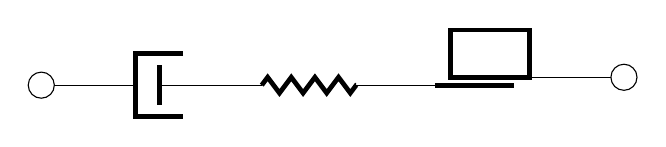
\begin{tikzpicture}[scale=2]
\draw(1.8,0)node[circle,draw,fill=white]{}--(2.4,0)(2.55,0)--(3.2,0)(3.8,0)--++(.6,0)(4.9,.05)--++(.6,0)node[circle,draw,fill=white]{};
\draw[line width=.6mm](2.7,.2)--++(-.3,0)--++(0,-.4)--++(.3,0)(2.55,.125)--++(0,-.25)(4.3,0)--++(.5,0)(4.4,.05)rectangle(4.9,.35);
\draw[line width=.6mm,decorate,decoration={zigzag,segment length=3mm, amplitude=1mm}](3.2,0)--++(.6,0);
\end{tikzpicture}
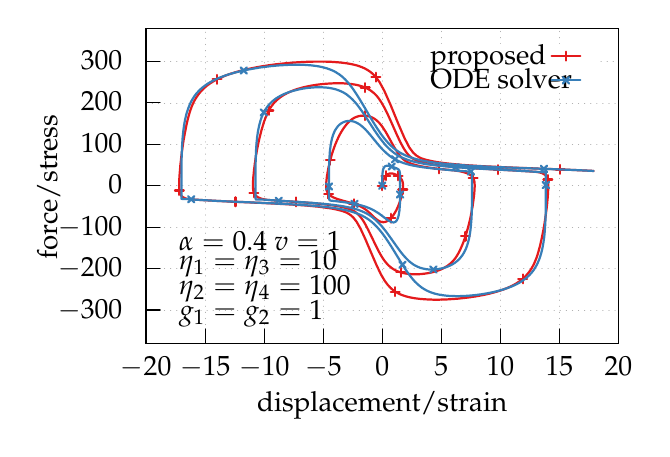
\begin{tikzpicture}[gnuplot]
%% generated with GNUPLOT 5.4p2 (Lua 5.4; terminal rev. Jun 2020, script rev. 114)
%% 11/05/21 19:46:12
\path (0.000,0.000) rectangle (6.000,4.000);
\gpcolor{color=gp lt color axes}
\gpsetlinetype{gp lt axes}
\gpsetdashtype{gp dt axes}
\gpsetlinewidth{0.50}
\draw[gp path] (0.000,0.421)--(5.999,0.421);
\gpcolor{color=gp lt color border}
\gpsetlinetype{gp lt border}
\gpsetdashtype{gp dt solid}
\gpsetlinewidth{1.00}
\draw[gp path] (0.000,0.421)--(0.180,0.421);
\node[gp node right] at (-0.184,0.421) {$-300$};
\gpcolor{color=gp lt color axes}
\gpsetlinetype{gp lt axes}
\gpsetdashtype{gp dt axes}
\gpsetlinewidth{0.50}
\draw[gp path] (0.000,0.947)--(5.999,0.947);
\gpcolor{color=gp lt color border}
\gpsetlinetype{gp lt border}
\gpsetdashtype{gp dt solid}
\gpsetlinewidth{1.00}
\draw[gp path] (0.000,0.947)--(0.180,0.947);
\node[gp node right] at (-0.184,0.947) {$-200$};
\gpcolor{color=gp lt color axes}
\gpsetlinetype{gp lt axes}
\gpsetdashtype{gp dt axes}
\gpsetlinewidth{0.50}
\draw[gp path] (0.000,1.473)--(5.999,1.473);
\gpcolor{color=gp lt color border}
\gpsetlinetype{gp lt border}
\gpsetdashtype{gp dt solid}
\gpsetlinewidth{1.00}
\draw[gp path] (0.000,1.473)--(0.180,1.473);
\node[gp node right] at (-0.184,1.473) {$-100$};
\gpcolor{color=gp lt color axes}
\gpsetlinetype{gp lt axes}
\gpsetdashtype{gp dt axes}
\gpsetlinewidth{0.50}
\draw[gp path] (0.000,2.000)--(5.999,2.000);
\gpcolor{color=gp lt color border}
\gpsetlinetype{gp lt border}
\gpsetdashtype{gp dt solid}
\gpsetlinewidth{1.00}
\draw[gp path] (0.000,2.000)--(0.180,2.000);
\node[gp node right] at (-0.184,2.000) {$0$};
\gpcolor{color=gp lt color axes}
\gpsetlinetype{gp lt axes}
\gpsetdashtype{gp dt axes}
\gpsetlinewidth{0.50}
\draw[gp path] (0.000,2.526)--(5.999,2.526);
\gpcolor{color=gp lt color border}
\gpsetlinetype{gp lt border}
\gpsetdashtype{gp dt solid}
\gpsetlinewidth{1.00}
\draw[gp path] (0.000,2.526)--(0.180,2.526);
\node[gp node right] at (-0.184,2.526) {$100$};
\gpcolor{color=gp lt color axes}
\gpsetlinetype{gp lt axes}
\gpsetdashtype{gp dt axes}
\gpsetlinewidth{0.50}
\draw[gp path] (0.000,3.052)--(5.999,3.052);
\gpcolor{color=gp lt color border}
\gpsetlinetype{gp lt border}
\gpsetdashtype{gp dt solid}
\gpsetlinewidth{1.00}
\draw[gp path] (0.000,3.052)--(0.180,3.052);
\node[gp node right] at (-0.184,3.052) {$200$};
\gpcolor{color=gp lt color axes}
\gpsetlinetype{gp lt axes}
\gpsetdashtype{gp dt axes}
\gpsetlinewidth{0.50}
\draw[gp path] (0.000,3.578)--(3.495,3.578);
\draw[gp path] (5.699,3.578)--(5.999,3.578);
\gpcolor{color=gp lt color border}
\gpsetlinetype{gp lt border}
\gpsetdashtype{gp dt solid}
\gpsetlinewidth{1.00}
\draw[gp path] (0.000,3.578)--(0.180,3.578);
\node[gp node right] at (-0.184,3.578) {$300$};
\gpcolor{color=gp lt color axes}
\gpsetlinetype{gp lt axes}
\gpsetdashtype{gp dt axes}
\gpsetlinewidth{0.50}
\draw[gp path] (0.000,0.000)--(0.000,3.999);
\gpcolor{color=gp lt color border}
\gpsetlinetype{gp lt border}
\gpsetdashtype{gp dt solid}
\gpsetlinewidth{1.00}
\draw[gp path] (0.000,0.000)--(0.000,0.180);
\node[gp node center] at (0.000,-0.308) {$-20$};
\gpcolor{color=gp lt color axes}
\gpsetlinetype{gp lt axes}
\gpsetdashtype{gp dt axes}
\gpsetlinewidth{0.50}
\draw[gp path] (0.750,0.000)--(0.750,3.999);
\gpcolor{color=gp lt color border}
\gpsetlinetype{gp lt border}
\gpsetdashtype{gp dt solid}
\gpsetlinewidth{1.00}
\draw[gp path] (0.750,0.000)--(0.750,0.180);
\node[gp node center] at (0.750,-0.308) {$-15$};
\gpcolor{color=gp lt color axes}
\gpsetlinetype{gp lt axes}
\gpsetdashtype{gp dt axes}
\gpsetlinewidth{0.50}
\draw[gp path] (1.500,0.000)--(1.500,3.999);
\gpcolor{color=gp lt color border}
\gpsetlinetype{gp lt border}
\gpsetdashtype{gp dt solid}
\gpsetlinewidth{1.00}
\draw[gp path] (1.500,0.000)--(1.500,0.180);
\node[gp node center] at (1.500,-0.308) {$-10$};
\gpcolor{color=gp lt color axes}
\gpsetlinetype{gp lt axes}
\gpsetdashtype{gp dt axes}
\gpsetlinewidth{0.50}
\draw[gp path] (2.250,0.000)--(2.250,3.999);
\gpcolor{color=gp lt color border}
\gpsetlinetype{gp lt border}
\gpsetdashtype{gp dt solid}
\gpsetlinewidth{1.00}
\draw[gp path] (2.250,0.000)--(2.250,0.180);
\node[gp node center] at (2.250,-0.308) {$-5$};
\gpcolor{color=gp lt color axes}
\gpsetlinetype{gp lt axes}
\gpsetdashtype{gp dt axes}
\gpsetlinewidth{0.50}
\draw[gp path] (3.000,0.000)--(3.000,3.999);
\gpcolor{color=gp lt color border}
\gpsetlinetype{gp lt border}
\gpsetdashtype{gp dt solid}
\gpsetlinewidth{1.00}
\draw[gp path] (3.000,0.000)--(3.000,0.180);
\node[gp node center] at (3.000,-0.308) {$0$};
\gpcolor{color=gp lt color axes}
\gpsetlinetype{gp lt axes}
\gpsetdashtype{gp dt axes}
\gpsetlinewidth{0.50}
\draw[gp path] (3.749,0.000)--(3.749,3.183);
\draw[gp path] (3.749,3.799)--(3.749,3.999);
\gpcolor{color=gp lt color border}
\gpsetlinetype{gp lt border}
\gpsetdashtype{gp dt solid}
\gpsetlinewidth{1.00}
\draw[gp path] (3.749,0.000)--(3.749,0.180);
\node[gp node center] at (3.749,-0.308) {$5$};
\gpcolor{color=gp lt color axes}
\gpsetlinetype{gp lt axes}
\gpsetdashtype{gp dt axes}
\gpsetlinewidth{0.50}
\draw[gp path] (4.499,0.000)--(4.499,3.183);
\draw[gp path] (4.499,3.799)--(4.499,3.999);
\gpcolor{color=gp lt color border}
\gpsetlinetype{gp lt border}
\gpsetdashtype{gp dt solid}
\gpsetlinewidth{1.00}
\draw[gp path] (4.499,0.000)--(4.499,0.180);
\node[gp node center] at (4.499,-0.308) {$10$};
\gpcolor{color=gp lt color axes}
\gpsetlinetype{gp lt axes}
\gpsetdashtype{gp dt axes}
\gpsetlinewidth{0.50}
\draw[gp path] (5.249,0.000)--(5.249,3.183);
\draw[gp path] (5.249,3.799)--(5.249,3.999);
\gpcolor{color=gp lt color border}
\gpsetlinetype{gp lt border}
\gpsetdashtype{gp dt solid}
\gpsetlinewidth{1.00}
\draw[gp path] (5.249,0.000)--(5.249,0.180);
\node[gp node center] at (5.249,-0.308) {$15$};
\gpcolor{color=gp lt color axes}
\gpsetlinetype{gp lt axes}
\gpsetdashtype{gp dt axes}
\gpsetlinewidth{0.50}
\draw[gp path] (5.999,0.000)--(5.999,3.999);
\gpcolor{color=gp lt color border}
\gpsetlinetype{gp lt border}
\gpsetdashtype{gp dt solid}
\gpsetlinewidth{1.00}
\draw[gp path] (5.999,0.000)--(5.999,0.180);
\node[gp node center] at (5.999,-0.308) {$20$};
\draw[gp path] (0.000,3.999)--(0.000,0.000)--(5.999,0.000)--(5.999,3.999)--cycle;
\node[gp node left] at (0.300,1.280) {$\alpha=0.4$ $v=1$};
\node[gp node left] at (0.300,1.040) {$\eta_1=\eta_3=10$};
\node[gp node left] at (0.300,0.720) {$\eta_2=\eta_4=100$};
\node[gp node left] at (0.300,0.400) {$g_1=g_2=1$};
\node[gp node center,rotate=-270] at (-1.212,1.999) {force/stress};
\node[gp node center] at (2.999,-0.769) {displacement/strain};
\gpcolor{rgb color={0.894,0.102,0.110}}
\gpsetlinewidth{2.00}
\draw[gp path] (3.000,2.000)--(3.000,2.001)--(3.000,2.002)--(3.000,2.003)--(3.000,2.004)%
  --(3.000,2.005)--(3.000,2.006)--(3.000,2.007)--(3.000,2.008)--(3.000,2.009)--(3.000,2.011)%
  --(3.000,2.012)--(3.000,2.013)--(3.001,2.015)--(3.001,2.016)--(3.001,2.018)--(3.001,2.019)%
  --(3.001,2.021)--(3.002,2.022)--(3.002,2.024)--(3.002,2.026)--(3.002,2.027)--(3.003,2.029)%
  --(3.003,2.031)--(3.003,2.033)--(3.004,2.035)--(3.004,2.037)--(3.004,2.038)--(3.005,2.040)%
  --(3.005,2.042)--(3.006,2.044)--(3.006,2.046)--(3.007,2.048)--(3.007,2.050)--(3.008,2.052)%
  --(3.008,2.054)--(3.009,2.056)--(3.010,2.058)--(3.010,2.060)--(3.011,2.063)--(3.012,2.065)%
  --(3.012,2.067)--(3.013,2.069)--(3.014,2.071)--(3.015,2.073)--(3.015,2.075)--(3.016,2.077)%
  --(3.017,2.079)--(3.018,2.081)--(3.019,2.083)--(3.020,2.085)--(3.021,2.087)--(3.022,2.089)%
  --(3.023,2.091)--(3.024,2.093)--(3.025,2.095)--(3.026,2.097)--(3.027,2.099)--(3.028,2.101)%
  --(3.029,2.103)--(3.030,2.105)--(3.031,2.107)--(3.032,2.109)--(3.034,2.111)--(3.035,2.113)%
  --(3.036,2.114)--(3.037,2.116)--(3.039,2.118)--(3.040,2.119)--(3.042,2.121)--(3.043,2.123)%
  --(3.044,2.124)--(3.046,2.126)--(3.047,2.127)--(3.049,2.129)--(3.050,2.130)--(3.052,2.132)%
  --(3.053,2.133)--(3.055,2.135)--(3.056,2.136)--(3.058,2.137)--(3.060,2.138)--(3.061,2.140)%
  --(3.063,2.141)--(3.065,2.142)--(3.066,2.143)--(3.068,2.144)--(3.070,2.145)--(3.072,2.146)%
  --(3.073,2.147)--(3.075,2.148)--(3.077,2.148)--(3.079,2.149)--(3.081,2.150)--(3.083,2.150)%
  --(3.085,2.151)--(3.086,2.152)--(3.088,2.152)--(3.090,2.153)--(3.092,2.153)--(3.094,2.153)%
  --(3.096,2.154)--(3.098,2.154)--(3.100,2.154)--(3.102,2.155)--(3.104,2.155)--(3.106,2.155)%
  --(3.108,2.155)--(3.111,2.155)--(3.113,2.155)--(3.115,2.155)--(3.117,2.155)--(3.119,2.155)%
  --(3.121,2.155)--(3.123,2.154)--(3.125,2.154)--(3.127,2.154)--(3.129,2.154)--(3.132,2.153)%
  --(3.134,2.153)--(3.136,2.152)--(3.138,2.152)--(3.140,2.151)--(3.142,2.151)--(3.144,2.150)%
  --(3.146,2.150)--(3.149,2.149)--(3.151,2.149)--(3.153,2.148)--(3.155,2.147)--(3.157,2.146)%
  --(3.159,2.146)--(3.161,2.145)--(3.163,2.144)--(3.165,2.143)--(3.168,2.142)--(3.170,2.142)%
  --(3.172,2.141)--(3.174,2.140)--(3.176,2.139)--(3.178,2.138)--(3.180,2.137)--(3.182,2.136)%
  --(3.184,2.135)--(3.186,2.134)--(3.188,2.133)--(3.190,2.131)--(3.191,2.130)--(3.193,2.129)%
  --(3.195,2.128)--(3.197,2.127)--(3.199,2.126)--(3.201,2.125)--(3.203,2.123)--(3.204,2.122)%
  --(3.206,2.121)--(3.208,2.120)--(3.210,2.118)--(3.211,2.117)--(3.213,2.116)--(3.215,2.114)%
  --(3.216,2.113)--(3.218,2.112)--(3.220,2.110)--(3.221,2.109)--(3.223,2.107)--(3.224,2.106)%
  --(3.226,2.104)--(3.227,2.103)--(3.229,2.101)--(3.230,2.100)--(3.232,2.098)--(3.233,2.097)%
  --(3.234,2.095)--(3.236,2.094)--(3.237,2.092)--(3.238,2.090)--(3.239,2.089)--(3.241,2.087)%
  --(3.242,2.085)--(3.243,2.084)--(3.244,2.082)--(3.245,2.080)--(3.246,2.078)--(3.247,2.077)%
  --(3.248,2.075)--(3.249,2.073)--(3.250,2.071)--(3.251,2.069)--(3.252,2.067)--(3.253,2.065)%
  --(3.254,2.063)--(3.254,2.061)--(3.255,2.059)--(3.256,2.057)--(3.257,2.055)--(3.257,2.053)%
  --(3.258,2.051)--(3.258,2.048)--(3.259,2.046)--(3.260,2.044)--(3.260,2.042)--(3.261,2.039)%
  --(3.261,2.037)--(3.261,2.034)--(3.262,2.032)--(3.262,2.029)--(3.262,2.027)--(3.263,2.024)%
  --(3.263,2.022)--(3.263,2.019)--(3.263,2.016)--(3.264,2.014)--(3.264,2.011)--(3.264,2.008)%
  --(3.264,2.005)--(3.264,2.002)--(3.264,1.999)--(3.264,1.996)--(3.264,1.993)--(3.264,1.990)%
  --(3.264,1.987)--(3.264,1.983)--(3.263,1.980)--(3.263,1.977)--(3.263,1.973)--(3.263,1.970)%
  --(3.262,1.967)--(3.262,1.963)--(3.262,1.959)--(3.261,1.956)--(3.261,1.952)--(3.260,1.948)%
  --(3.260,1.945)--(3.259,1.941)--(3.259,1.937)--(3.258,1.933)--(3.258,1.929)--(3.257,1.925)%
  --(3.256,1.921)--(3.255,1.917)--(3.255,1.913)--(3.254,1.909)--(3.253,1.904)--(3.252,1.900)%
  --(3.251,1.896)--(3.250,1.892)--(3.249,1.887)--(3.248,1.883)--(3.247,1.878)--(3.246,1.874)%
  --(3.245,1.869)--(3.244,1.865)--(3.243,1.860)--(3.242,1.855)--(3.240,1.851)--(3.239,1.846)%
  --(3.238,1.841)--(3.236,1.836)--(3.235,1.831)--(3.234,1.827)--(3.232,1.822)--(3.231,1.817)%
  --(3.229,1.812)--(3.227,1.807)--(3.226,1.802)--(3.224,1.797)--(3.222,1.792)--(3.221,1.787)%
  --(3.219,1.782)--(3.217,1.777)--(3.215,1.772)--(3.213,1.767)--(3.211,1.762)--(3.209,1.757)%
  --(3.207,1.751)--(3.205,1.746)--(3.203,1.741)--(3.201,1.736)--(3.199,1.731)--(3.197,1.726)%
  --(3.194,1.721)--(3.192,1.716)--(3.190,1.711)--(3.187,1.706)--(3.185,1.701)--(3.182,1.695)%
  --(3.180,1.690)--(3.177,1.685)--(3.175,1.680)--(3.172,1.676)--(3.169,1.671)--(3.167,1.666)%
  --(3.164,1.661)--(3.161,1.656)--(3.158,1.651)--(3.155,1.646)--(3.152,1.642)--(3.149,1.637)%
  --(3.146,1.632)--(3.143,1.628)--(3.140,1.623)--(3.136,1.619)--(3.133,1.614)--(3.130,1.610)%
  --(3.126,1.606)--(3.123,1.602)--(3.119,1.598)--(3.116,1.594)--(3.112,1.590)--(3.109,1.586)%
  --(3.105,1.582)--(3.101,1.578)--(3.097,1.575)--(3.094,1.571)--(3.090,1.568)--(3.086,1.565)%
  --(3.082,1.562)--(3.077,1.559)--(3.073,1.556)--(3.069,1.553)--(3.065,1.551)--(3.060,1.548)%
  --(3.056,1.546)--(3.051,1.544)--(3.047,1.542)--(3.042,1.541)--(3.037,1.539)--(3.032,1.538)%
  --(3.027,1.537)--(3.022,1.537)--(3.017,1.536)--(3.012,1.536)--(3.006,1.536)--(3.001,1.537)%
  --(2.995,1.538)--(2.990,1.539)--(2.984,1.541)--(2.978,1.543)--(2.972,1.545)--(2.966,1.548)%
  --(2.960,1.551)--(2.953,1.554)--(2.947,1.558)--(2.940,1.563)--(2.933,1.568)--(2.926,1.573)%
  --(2.919,1.579)--(2.912,1.585)--(2.904,1.592)--(2.897,1.599)--(2.889,1.606)--(2.882,1.614)%
  --(2.874,1.621)--(2.866,1.629)--(2.859,1.636)--(2.851,1.643)--(2.844,1.650)--(2.836,1.657)%
  --(2.829,1.664)--(2.821,1.670)--(2.814,1.676)--(2.807,1.682)--(2.800,1.688)--(2.793,1.693)%
  --(2.786,1.698)--(2.779,1.703)--(2.772,1.707)--(2.766,1.712)--(2.759,1.716)--(2.752,1.720)%
  --(2.746,1.724)--(2.739,1.727)--(2.733,1.731)--(2.727,1.734)--(2.720,1.737)--(2.714,1.740)%
  --(2.708,1.743)--(2.702,1.745)--(2.695,1.748)--(2.689,1.751)--(2.683,1.753)--(2.677,1.755)%
  --(2.671,1.758)--(2.666,1.760)--(2.660,1.762)--(2.654,1.764)--(2.648,1.766)--(2.642,1.768)%
  --(2.637,1.770)--(2.631,1.772)--(2.625,1.773)--(2.620,1.775)--(2.614,1.777)--(2.608,1.779)%
  --(2.603,1.780)--(2.597,1.782)--(2.592,1.783)--(2.587,1.785)--(2.581,1.787)--(2.576,1.788)%
  --(2.571,1.789)--(2.565,1.791)--(2.560,1.792)--(2.555,1.794)--(2.550,1.795)--(2.545,1.797)%
  --(2.540,1.798)--(2.535,1.799)--(2.530,1.801)--(2.525,1.802)--(2.520,1.804)--(2.515,1.805)%
  --(2.510,1.806)--(2.505,1.808)--(2.500,1.809)--(2.496,1.810)--(2.491,1.812)--(2.486,1.813)%
  --(2.482,1.814)--(2.477,1.816)--(2.473,1.817)--(2.468,1.818)--(2.464,1.820)--(2.460,1.821)%
  --(2.455,1.822)--(2.451,1.824)--(2.447,1.825)--(2.443,1.826)--(2.438,1.828)--(2.434,1.829)%
  --(2.430,1.831)--(2.426,1.832)--(2.422,1.833)--(2.418,1.835)--(2.415,1.836)--(2.411,1.838)%
  --(2.407,1.839)--(2.403,1.841)--(2.400,1.842)--(2.396,1.844)--(2.393,1.845)--(2.389,1.847)%
  --(2.386,1.848)--(2.382,1.850)--(2.379,1.851)--(2.376,1.853)--(2.373,1.855)--(2.370,1.856)%
  --(2.366,1.858)--(2.363,1.859)--(2.361,1.861)--(2.358,1.863)--(2.355,1.864)--(2.352,1.866)%
  --(2.349,1.868)--(2.347,1.870)--(2.344,1.872)--(2.341,1.873)--(2.339,1.875)--(2.336,1.877)%
  --(2.334,1.879)--(2.332,1.881)--(2.330,1.883)--(2.327,1.885)--(2.325,1.887)--(2.323,1.889)%
  --(2.321,1.891)--(2.319,1.893)--(2.317,1.895)--(2.316,1.897)--(2.314,1.899)--(2.312,1.902)%
  --(2.310,1.904)--(2.309,1.906)--(2.307,1.909)--(2.306,1.911)--(2.305,1.914)--(2.303,1.916)%
  --(2.302,1.919)--(2.301,1.921)--(2.300,1.924)--(2.299,1.927)--(2.298,1.930)--(2.297,1.933)%
  --(2.296,1.936)--(2.295,1.939)--(2.294,1.942)--(2.293,1.945)--(2.293,1.948)--(2.292,1.952)%
  --(2.291,1.955)--(2.291,1.959)--(2.290,1.962)--(2.290,1.966)--(2.290,1.970)--(2.289,1.974)%
  --(2.289,1.978)--(2.289,1.982)--(2.289,1.986)--(2.288,1.991)--(2.288,1.995)--(2.288,2.000)%
  --(2.288,2.005)--(2.288,2.010)--(2.289,2.015)--(2.289,2.020)--(2.289,2.025)--(2.289,2.030)%
  --(2.290,2.036)--(2.290,2.041)--(2.290,2.047)--(2.291,2.053)--(2.291,2.059)--(2.292,2.065)%
  --(2.293,2.071)--(2.293,2.077)--(2.294,2.084)--(2.295,2.090)--(2.295,2.097)--(2.296,2.104)%
  --(2.297,2.110)--(2.298,2.117)--(2.299,2.125)--(2.300,2.132)--(2.301,2.139)--(2.303,2.147)%
  --(2.304,2.154)--(2.305,2.162)--(2.306,2.169)--(2.308,2.177)--(2.309,2.185)--(2.311,2.193)%
  --(2.312,2.201)--(2.314,2.210)--(2.315,2.218)--(2.317,2.226)--(2.319,2.235)--(2.321,2.243)%
  --(2.323,2.252)--(2.325,2.261)--(2.327,2.270)--(2.329,2.279)--(2.331,2.287)--(2.333,2.296)%
  --(2.335,2.306)--(2.337,2.315)--(2.340,2.324)--(2.342,2.333)--(2.345,2.342)--(2.347,2.352)%
  --(2.350,2.361)--(2.353,2.371)--(2.355,2.380)--(2.358,2.390)--(2.361,2.399)--(2.364,2.409)%
  --(2.367,2.418)--(2.370,2.428)--(2.373,2.438)--(2.376,2.447)--(2.380,2.457)--(2.383,2.467)%
  --(2.387,2.476)--(2.390,2.486)--(2.394,2.496)--(2.397,2.506)--(2.401,2.515)--(2.405,2.525)%
  --(2.409,2.535)--(2.413,2.544)--(2.417,2.554)--(2.421,2.563)--(2.425,2.573)--(2.429,2.583)%
  --(2.434,2.592)--(2.438,2.601)--(2.442,2.611)--(2.447,2.620)--(2.452,2.630)--(2.456,2.639)%
  --(2.461,2.648)--(2.466,2.657)--(2.471,2.666)--(2.476,2.675)--(2.481,2.684)--(2.487,2.693)%
  --(2.492,2.701)--(2.497,2.710)--(2.503,2.718)--(2.508,2.727)--(2.514,2.735)--(2.520,2.743)%
  --(2.526,2.751)--(2.532,2.759)--(2.538,2.767)--(2.544,2.774)--(2.550,2.782)--(2.556,2.789)%
  --(2.563,2.796)--(2.569,2.803)--(2.576,2.809)--(2.583,2.816)--(2.590,2.822)--(2.597,2.828)%
  --(2.604,2.834)--(2.611,2.840)--(2.618,2.845)--(2.626,2.850)--(2.633,2.854)--(2.641,2.859)%
  --(2.649,2.863)--(2.657,2.867)--(2.665,2.870)--(2.673,2.874)--(2.681,2.876)--(2.690,2.879)%
  --(2.698,2.881)--(2.707,2.884)--(2.716,2.885)--(2.725,2.887)--(2.734,2.888)--(2.743,2.889)%
  --(2.752,2.889)--(2.762,2.890)--(2.771,2.889)--(2.781,2.889)--(2.791,2.888)--(2.801,2.887)%
  --(2.811,2.885)--(2.821,2.883)--(2.831,2.880)--(2.842,2.877)--(2.853,2.874)--(2.864,2.869)%
  --(2.875,2.864)--(2.886,2.858)--(2.898,2.851)--(2.910,2.843)--(2.922,2.834)--(2.935,2.823)%
  --(2.949,2.810)--(2.963,2.796)--(2.977,2.779)--(2.993,2.759)--(3.009,2.737)--(3.026,2.710)%
  --(3.045,2.681)--(3.064,2.648)--(3.084,2.612)--(3.104,2.575)--(3.125,2.537)--(3.145,2.502)%
  --(3.164,2.468)--(3.183,2.439)--(3.200,2.413)--(3.216,2.390)--(3.231,2.371)--(3.246,2.355)%
  --(3.260,2.342)--(3.273,2.330)--(3.285,2.321)--(3.298,2.312)--(3.309,2.305)--(3.321,2.299)%
  --(3.332,2.293)--(3.344,2.288)--(3.355,2.284)--(3.366,2.279)--(3.376,2.276)--(3.387,2.272)%
  --(3.398,2.269)--(3.408,2.266)--(3.419,2.263)--(3.429,2.260)--(3.439,2.258)--(3.450,2.255)%
  --(3.460,2.253)--(3.470,2.251)--(3.480,2.248)--(3.490,2.246)--(3.500,2.244)--(3.510,2.243)%
  --(3.520,2.241)--(3.530,2.239)--(3.540,2.237)--(3.549,2.236)--(3.559,2.234)--(3.569,2.233)%
  --(3.578,2.231)--(3.588,2.230)--(3.597,2.228)--(3.606,2.227)--(3.616,2.226)--(3.625,2.225)%
  --(3.634,2.223)--(3.643,2.222)--(3.653,2.221)--(3.662,2.220)--(3.671,2.219)--(3.680,2.218)%
  --(3.688,2.217)--(3.697,2.216)--(3.706,2.215)--(3.715,2.214)--(3.723,2.213)--(3.732,2.212)%
  --(3.740,2.211)--(3.749,2.210)--(3.757,2.209)--(3.765,2.208)--(3.774,2.207)--(3.782,2.207)%
  --(3.790,2.206)--(3.798,2.205)--(3.806,2.204)--(3.814,2.203)--(3.822,2.203)--(3.829,2.202)%
  --(3.837,2.201)--(3.845,2.201)--(3.852,2.200)--(3.859,2.199)--(3.867,2.198)--(3.874,2.198)%
  --(3.881,2.197)--(3.888,2.196)--(3.895,2.195)--(3.902,2.195)--(3.909,2.194)--(3.916,2.193)%
  --(3.923,2.192)--(3.930,2.191)--(3.936,2.190)--(3.943,2.189)--(3.949,2.188)--(3.956,2.187)%
  --(3.962,2.186)--(3.968,2.185)--(3.974,2.184)--(3.980,2.183)--(3.986,2.182)--(3.992,2.181)%
  --(3.998,2.180)--(4.004,2.178)--(4.009,2.177)--(4.015,2.176)--(4.020,2.175)--(4.025,2.173)%
  --(4.031,2.172)--(4.036,2.170)--(4.041,2.169)--(4.046,2.168)--(4.051,2.166)--(4.056,2.164)%
  --(4.060,2.163)--(4.065,2.161)--(4.070,2.160)--(4.074,2.158)--(4.078,2.156)--(4.083,2.154)%
  --(4.087,2.153)--(4.091,2.151)--(4.095,2.149)--(4.099,2.147)--(4.102,2.145)--(4.106,2.143)%
  --(4.110,2.141)--(4.113,2.139)--(4.116,2.137)--(4.120,2.134)--(4.123,2.132)--(4.126,2.130)%
  --(4.129,2.128)--(4.132,2.125)--(4.135,2.123)--(4.137,2.120)--(4.140,2.118)--(4.142,2.115)%
  --(4.145,2.113)--(4.147,2.110)--(4.149,2.107)--(4.151,2.104)--(4.153,2.101)--(4.155,2.098)%
  --(4.157,2.095)--(4.158,2.092)--(4.160,2.089)--(4.161,2.086)--(4.163,2.082)--(4.164,2.079)%
  --(4.165,2.075)--(4.166,2.071)--(4.167,2.067)--(4.168,2.063)--(4.169,2.059)--(4.170,2.055)%
  --(4.171,2.050)--(4.171,2.046)--(4.172,2.041)--(4.172,2.036)--(4.173,2.031)--(4.173,2.025)%
  --(4.173,2.020)--(4.174,2.014)--(4.174,2.008)--(4.174,2.002)--(4.174,1.996)--(4.174,1.989)%
  --(4.174,1.982)--(4.173,1.975)--(4.173,1.968)--(4.173,1.961)--(4.172,1.953)--(4.172,1.945)%
  --(4.171,1.937)--(4.171,1.929)--(4.170,1.920)--(4.169,1.912)--(4.169,1.903)--(4.168,1.894)%
  --(4.167,1.884)--(4.166,1.875)--(4.165,1.865)--(4.164,1.855)--(4.162,1.845)--(4.161,1.835)%
  --(4.160,1.824)--(4.158,1.813)--(4.157,1.803)--(4.155,1.792)--(4.154,1.780)--(4.152,1.769)%
  --(4.150,1.757)--(4.149,1.746)--(4.147,1.734)--(4.145,1.722)--(4.142,1.709)--(4.140,1.697)%
  --(4.138,1.684)--(4.136,1.672)--(4.133,1.659)--(4.131,1.646)--(4.128,1.633)--(4.126,1.620)%
  --(4.123,1.607)--(4.120,1.593)--(4.117,1.580)--(4.114,1.566)--(4.111,1.553)--(4.108,1.539)%
  --(4.104,1.525)--(4.101,1.511)--(4.097,1.497)--(4.094,1.483)--(4.090,1.469)--(4.086,1.455)%
  --(4.082,1.441)--(4.078,1.427)--(4.074,1.413)--(4.070,1.399)--(4.066,1.385)--(4.061,1.370)%
  --(4.057,1.356)--(4.052,1.342)--(4.047,1.328)--(4.042,1.314)--(4.037,1.300)--(4.032,1.286)%
  --(4.027,1.272)--(4.021,1.258)--(4.016,1.244)--(4.010,1.231)--(4.004,1.217)--(3.998,1.204)%
  --(3.992,1.190)--(3.986,1.177)--(3.980,1.164)--(3.973,1.152)--(3.966,1.139)--(3.959,1.127)%
  --(3.952,1.115)--(3.945,1.103)--(3.938,1.092)--(3.930,1.081)--(3.922,1.070)--(3.914,1.060)%
  --(3.906,1.051)--(3.897,1.041)--(3.889,1.032)--(3.880,1.024)--(3.871,1.015)--(3.862,1.007)%
  --(3.852,1.000)--(3.843,0.992)--(3.833,0.985)--(3.823,0.978)--(3.813,0.972)--(3.803,0.966)%
  --(3.793,0.960)--(3.782,0.954)--(3.772,0.948)--(3.761,0.943)--(3.750,0.938)--(3.739,0.933)%
  --(3.728,0.929)--(3.716,0.924)--(3.705,0.920)--(3.693,0.916)--(3.682,0.912)--(3.670,0.909)%
  --(3.658,0.906)--(3.646,0.902)--(3.634,0.899)--(3.621,0.896)--(3.609,0.894)--(3.597,0.891)%
  --(3.584,0.889)--(3.571,0.887)--(3.558,0.885)--(3.546,0.883)--(3.533,0.881)--(3.519,0.880)%
  --(3.506,0.878)--(3.493,0.877)--(3.480,0.876)--(3.466,0.875)--(3.452,0.875)--(3.439,0.875)%
  --(3.425,0.874)--(3.411,0.874)--(3.397,0.875)--(3.383,0.875)--(3.369,0.876)--(3.354,0.877)%
  --(3.340,0.878)--(3.325,0.880)--(3.311,0.882)--(3.296,0.884)--(3.281,0.887)--(3.266,0.890)%
  --(3.250,0.894)--(3.235,0.899)--(3.219,0.904)--(3.203,0.909)--(3.187,0.916)--(3.170,0.924)%
  --(3.154,0.932)--(3.136,0.943)--(3.118,0.955)--(3.100,0.970)--(3.080,0.987)--(3.060,1.008)%
  --(3.038,1.034)--(3.014,1.067)--(2.988,1.108)--(2.959,1.159)--(2.927,1.222)--(2.892,1.294)%
  --(2.856,1.369)--(2.821,1.440)--(2.790,1.500)--(2.762,1.549)--(2.736,1.586)--(2.714,1.615)%
  --(2.693,1.636)--(2.674,1.653)--(2.656,1.667)--(2.639,1.677)--(2.622,1.686)--(2.605,1.693)%
  --(2.589,1.700)--(2.573,1.705)--(2.558,1.710)--(2.542,1.715)--(2.527,1.719)--(2.511,1.723)%
  --(2.496,1.726)--(2.481,1.730)--(2.466,1.733)--(2.451,1.736)--(2.436,1.738)--(2.422,1.741)%
  --(2.407,1.743)--(2.392,1.746)--(2.378,1.748)--(2.364,1.750)--(2.349,1.752)--(2.335,1.754)%
  --(2.321,1.756)--(2.306,1.758)--(2.292,1.760)--(2.278,1.761)--(2.264,1.763)--(2.251,1.764)%
  --(2.237,1.766)--(2.223,1.767)--(2.209,1.769)--(2.196,1.770)--(2.182,1.771)--(2.169,1.773)%
  --(2.156,1.774)--(2.142,1.775)--(2.129,1.776)--(2.116,1.778)--(2.103,1.779)--(2.090,1.780)%
  --(2.077,1.781)--(2.064,1.782)--(2.052,1.783)--(2.039,1.784)--(2.026,1.785)--(2.014,1.786)%
  --(2.002,1.787)--(1.989,1.788)--(1.977,1.789)--(1.965,1.789)--(1.953,1.790)--(1.941,1.791)%
  --(1.929,1.792)--(1.918,1.793)--(1.906,1.794)--(1.894,1.794)--(1.883,1.795)--(1.872,1.796)%
  --(1.860,1.797)--(1.849,1.798)--(1.838,1.798)--(1.827,1.799)--(1.817,1.800)--(1.806,1.801)%
  --(1.795,1.801)--(1.785,1.802)--(1.774,1.803)--(1.764,1.803)--(1.754,1.804)--(1.744,1.805)%
  --(1.734,1.805)--(1.724,1.806)--(1.715,1.807)--(1.705,1.807)--(1.696,1.808)--(1.686,1.809)%
  --(1.677,1.809)--(1.668,1.810)--(1.659,1.810)--(1.651,1.811)--(1.642,1.812)--(1.633,1.812)%
  --(1.625,1.813)--(1.617,1.813)--(1.609,1.814)--(1.601,1.815)--(1.593,1.815)--(1.585,1.816)%
  --(1.577,1.816)--(1.570,1.817)--(1.563,1.817)--(1.555,1.818)--(1.548,1.819)--(1.541,1.819)%
  --(1.534,1.820)--(1.528,1.821)--(1.521,1.822)--(1.515,1.823)--(1.508,1.824)--(1.502,1.825)%
  --(1.496,1.827)--(1.490,1.828)--(1.484,1.829)--(1.478,1.831)--(1.473,1.832)--(1.467,1.834)%
  --(1.462,1.836)--(1.457,1.837)--(1.452,1.839)--(1.447,1.841)--(1.442,1.843)--(1.438,1.845)%
  --(1.433,1.847)--(1.429,1.849)--(1.424,1.851)--(1.420,1.854)--(1.416,1.856)--(1.412,1.859)%
  --(1.409,1.861)--(1.405,1.864)--(1.402,1.866)--(1.399,1.869)--(1.395,1.872)--(1.392,1.875)%
  --(1.390,1.878)--(1.387,1.881)--(1.384,1.884)--(1.382,1.887)--(1.379,1.891)--(1.377,1.894)%
  --(1.375,1.898)--(1.373,1.902)--(1.372,1.905)--(1.370,1.909)--(1.368,1.914)--(1.367,1.918)%
  --(1.366,1.922)--(1.364,1.927)--(1.363,1.932)--(1.363,1.937)--(1.362,1.942)--(1.361,1.948)%
  --(1.360,1.953)--(1.360,1.959)--(1.359,1.966)--(1.359,1.972)--(1.359,1.979)--(1.358,1.986)%
  --(1.358,1.994)--(1.358,2.002)--(1.358,2.010)--(1.359,2.018)--(1.359,2.027)--(1.359,2.036)%
  --(1.360,2.045)--(1.360,2.055)--(1.360,2.065)--(1.361,2.075)--(1.362,2.086)--(1.363,2.097)%
  --(1.363,2.108)--(1.364,2.120)--(1.365,2.132)--(1.367,2.144)--(1.368,2.156)--(1.369,2.169)%
  --(1.370,2.182)--(1.372,2.196)--(1.373,2.209)--(1.375,2.223)--(1.377,2.237)--(1.379,2.252)%
  --(1.380,2.267)--(1.382,2.282)--(1.385,2.297)--(1.387,2.312)--(1.389,2.328)--(1.391,2.344)%
  --(1.394,2.360)--(1.397,2.376)--(1.399,2.393)--(1.402,2.409)--(1.405,2.426)--(1.408,2.443)%
  --(1.411,2.461)--(1.415,2.478)--(1.418,2.495)--(1.422,2.513)--(1.425,2.531)--(1.429,2.549)%
  --(1.433,2.567)--(1.437,2.585)--(1.441,2.603)--(1.446,2.621)--(1.450,2.639)--(1.455,2.658)%
  --(1.459,2.676)--(1.464,2.694)--(1.469,2.713)--(1.475,2.731)--(1.480,2.749)--(1.486,2.768)%
  --(1.491,2.786)--(1.497,2.804)--(1.503,2.822)--(1.510,2.840)--(1.516,2.857)--(1.523,2.874)%
  --(1.530,2.891)--(1.537,2.908)--(1.544,2.924)--(1.552,2.940)--(1.560,2.955)--(1.568,2.970)%
  --(1.577,2.984)--(1.586,2.997)--(1.595,3.011)--(1.605,3.023)--(1.614,3.036)--(1.624,3.047)%
  --(1.634,3.059)--(1.645,3.069)--(1.655,3.080)--(1.666,3.090)--(1.678,3.100)--(1.689,3.109)%
  --(1.701,3.118)--(1.713,3.127)--(1.725,3.135)--(1.737,3.143)--(1.749,3.151)--(1.762,3.158)%
  --(1.775,3.165)--(1.788,3.172)--(1.801,3.179)--(1.815,3.185)--(1.828,3.191)--(1.842,3.197)%
  --(1.856,3.203)--(1.870,3.209)--(1.884,3.214)--(1.899,3.219)--(1.914,3.224)--(1.928,3.229)%
  --(1.943,3.233)--(1.958,3.237)--(1.974,3.242)--(1.989,3.246)--(2.004,3.250)--(2.020,3.253)%
  --(2.036,3.257)--(2.052,3.260)--(2.068,3.264)--(2.084,3.267)--(2.100,3.270)--(2.116,3.273)%
  --(2.133,3.275)--(2.149,3.278)--(2.166,3.281)--(2.183,3.283)--(2.200,3.285)--(2.217,3.287)%
  --(2.234,3.289)--(2.252,3.291)--(2.269,3.292)--(2.287,3.294)--(2.304,3.295)--(2.322,3.296)%
  --(2.340,3.298)--(2.358,3.298)--(2.376,3.299)--(2.394,3.300)--(2.412,3.300)--(2.430,3.300)%
  --(2.449,3.300)--(2.467,3.300)--(2.486,3.299)--(2.505,3.299)--(2.524,3.298)--(2.543,3.296)%
  --(2.562,3.295)--(2.581,3.293)--(2.601,3.291)--(2.620,3.288)--(2.640,3.285)--(2.660,3.282)%
  --(2.680,3.278)--(2.700,3.273)--(2.721,3.267)--(2.741,3.261)--(2.762,3.254)--(2.784,3.245)%
  --(2.806,3.235)--(2.828,3.223)--(2.851,3.209)--(2.875,3.191)--(2.901,3.170)--(2.928,3.142)%
  --(2.957,3.106)--(2.990,3.056)--(3.029,2.988)--(3.075,2.894)--(3.127,2.779)--(3.180,2.659)%
  --(3.228,2.556)--(3.269,2.480)--(3.303,2.427)--(3.332,2.391)--(3.359,2.366)--(3.383,2.348)%
  --(3.405,2.334)--(3.427,2.324)--(3.449,2.315)--(3.470,2.308)--(3.490,2.302)--(3.511,2.297)%
  --(3.531,2.292)--(3.551,2.287)--(3.571,2.283)--(3.591,2.279)--(3.611,2.275)--(3.630,2.272)%
  --(3.650,2.269)--(3.669,2.266)--(3.688,2.263)--(3.707,2.261)--(3.727,2.258)--(3.746,2.256)%
  --(3.765,2.254)--(3.783,2.252)--(3.802,2.250)--(3.821,2.248)--(3.839,2.246)--(3.858,2.244)%
  --(3.876,2.242)--(3.895,2.241)--(3.913,2.239)--(3.931,2.237)--(3.949,2.236)--(3.967,2.235)%
  --(3.985,2.233)--(4.003,2.232)--(4.020,2.231)--(4.038,2.229)--(4.056,2.228)--(4.073,2.227)%
  --(4.090,2.226)--(4.107,2.225)--(4.125,2.224)--(4.142,2.222)--(4.158,2.221)--(4.175,2.220)%
  --(4.192,2.219)--(4.209,2.218)--(4.225,2.217)--(4.241,2.216)--(4.258,2.215)--(4.274,2.215)%
  --(4.290,2.214)--(4.306,2.213)--(4.321,2.212)--(4.337,2.211)--(4.353,2.210)--(4.368,2.209)%
  --(4.383,2.208)--(4.399,2.208)--(4.414,2.207)--(4.429,2.206)--(4.443,2.205)--(4.458,2.204)%
  --(4.472,2.204)--(4.487,2.203)--(4.501,2.202)--(4.515,2.201)--(4.529,2.201)--(4.543,2.200)%
  --(4.557,2.199)--(4.570,2.198)--(4.584,2.198)--(4.597,2.197)--(4.610,2.196)--(4.623,2.196)%
  --(4.636,2.195)--(4.648,2.194)--(4.661,2.193)--(4.673,2.193)--(4.685,2.192)--(4.697,2.191)%
  --(4.709,2.191)--(4.721,2.190)--(4.732,2.189)--(4.744,2.189)--(4.755,2.188)--(4.766,2.187)%
  --(4.777,2.187)--(4.787,2.186)--(4.798,2.185)--(4.808,2.185)--(4.818,2.184)--(4.828,2.183)%
  --(4.838,2.183)--(4.848,2.182)--(4.857,2.181)--(4.866,2.181)--(4.876,2.180)--(4.884,2.180)%
  --(4.893,2.179)--(4.902,2.178)--(4.910,2.178)--(4.918,2.177)--(4.926,2.177)--(4.934,2.176)%
  --(4.941,2.176)--(4.949,2.175)--(4.956,2.174)--(4.963,2.174)--(4.970,2.173)--(4.977,2.172)%
  --(4.983,2.171)--(4.990,2.169)--(4.996,2.168)--(5.002,2.167)--(5.008,2.165)--(5.014,2.163)%
  --(5.019,2.162)--(5.025,2.160)--(5.030,2.158)--(5.035,2.156)--(5.040,2.153)--(5.045,2.151)%
  --(5.049,2.149)--(5.053,2.146)--(5.058,2.143)--(5.062,2.140)--(5.066,2.138)--(5.069,2.135)%
  --(5.073,2.131)--(5.076,2.128)--(5.079,2.125)--(5.082,2.121)--(5.085,2.118)--(5.088,2.114)%
  --(5.090,2.110)--(5.092,2.106)--(5.094,2.102)--(5.096,2.097)--(5.098,2.093)--(5.100,2.088)%
  --(5.101,2.083)--(5.103,2.078)--(5.104,2.072)--(5.105,2.066)--(5.106,2.060)--(5.106,2.054)%
  --(5.107,2.047)--(5.108,2.040)--(5.108,2.033)--(5.109,2.025)--(5.109,2.016)--(5.109,2.008)%
  --(5.109,1.999)--(5.109,1.989)--(5.109,1.979)--(5.109,1.969)--(5.108,1.958)--(5.108,1.947)%
  --(5.107,1.935)--(5.107,1.923)--(5.106,1.911)--(5.105,1.898)--(5.104,1.885)--(5.103,1.871)%
  --(5.102,1.857)--(5.101,1.842)--(5.100,1.827)--(5.098,1.812)--(5.097,1.796)--(5.095,1.780)%
  --(5.094,1.763)--(5.092,1.746)--(5.090,1.729)--(5.088,1.711)--(5.086,1.693)--(5.083,1.675)%
  --(5.081,1.656)--(5.078,1.637)--(5.076,1.618)--(5.073,1.598)--(5.070,1.579)--(5.067,1.559)%
  --(5.064,1.538)--(5.061,1.518)--(5.057,1.497)--(5.054,1.476)--(5.050,1.455)--(5.046,1.433)%
  --(5.042,1.412)--(5.038,1.390)--(5.033,1.368)--(5.029,1.346)--(5.024,1.324)--(5.019,1.302)%
  --(5.014,1.280)--(5.009,1.257)--(5.004,1.235)--(4.998,1.213)--(4.992,1.191)--(4.986,1.169)%
  --(4.980,1.147)--(4.973,1.125)--(4.966,1.104)--(4.959,1.083)--(4.951,1.063)--(4.943,1.043)%
  --(4.935,1.024)--(4.927,1.005)--(4.918,0.987)--(4.908,0.970)--(4.899,0.953)--(4.889,0.937)%
  --(4.878,0.921)--(4.868,0.906)--(4.856,0.892)--(4.845,0.878)--(4.833,0.865)--(4.821,0.852)%
  --(4.809,0.840)--(4.796,0.828)--(4.783,0.816)--(4.770,0.805)--(4.757,0.795)--(4.743,0.785)%
  --(4.729,0.775)--(4.714,0.766)--(4.700,0.756)--(4.685,0.748)--(4.670,0.739)--(4.654,0.731)%
  --(4.639,0.723)--(4.623,0.716)--(4.607,0.709)--(4.591,0.701)--(4.574,0.695)--(4.558,0.688)%
  --(4.541,0.682)--(4.524,0.676)--(4.506,0.670)--(4.489,0.664)--(4.471,0.658)--(4.453,0.653)%
  --(4.435,0.648)--(4.417,0.643)--(4.399,0.638)--(4.380,0.633)--(4.362,0.628)--(4.343,0.624)%
  --(4.324,0.620)--(4.304,0.615)--(4.285,0.611)--(4.265,0.608)--(4.246,0.604)--(4.226,0.600)%
  --(4.206,0.597)--(4.186,0.593)--(4.166,0.590)--(4.145,0.587)--(4.125,0.584)--(4.104,0.581)%
  --(4.083,0.578)--(4.062,0.576)--(4.041,0.573)--(4.020,0.571)--(3.998,0.569)--(3.977,0.566)%
  --(3.955,0.564)--(3.934,0.563)--(3.912,0.561)--(3.890,0.559)--(3.868,0.558)--(3.846,0.556)%
  --(3.823,0.555)--(3.801,0.554)--(3.778,0.554)--(3.756,0.553)--(3.733,0.552)--(3.710,0.552)%
  --(3.687,0.552)--(3.664,0.552)--(3.641,0.552)--(3.618,0.553)--(3.594,0.554)--(3.571,0.555)%
  --(3.547,0.556)--(3.523,0.558)--(3.499,0.560)--(3.475,0.562)--(3.451,0.565)--(3.426,0.568)%
  --(3.402,0.572)--(3.377,0.576)--(3.352,0.581)--(3.326,0.587)--(3.301,0.594)--(3.275,0.602)%
  --(3.248,0.612)--(3.221,0.623)--(3.194,0.637)--(3.165,0.654)--(3.135,0.675)--(3.104,0.703)%
  --(3.070,0.740)--(3.031,0.792)--(2.984,0.872)--(2.926,0.994)--(2.855,1.158)--(2.783,1.327)%
  --(2.723,1.456)--(2.676,1.539)--(2.637,1.590)--(2.605,1.621)--(2.575,1.642)--(2.547,1.657)%
  --(2.521,1.668)--(2.495,1.677)--(2.469,1.684)--(2.443,1.691)--(2.418,1.697)--(2.393,1.702)%
  --(2.369,1.707)--(2.344,1.711)--(2.320,1.715)--(2.295,1.718)--(2.271,1.722)--(2.247,1.725)%
  --(2.223,1.728)--(2.199,1.731)--(2.176,1.734)--(2.152,1.736)--(2.129,1.738)--(2.105,1.741)%
  --(2.082,1.743)--(2.059,1.745)--(2.035,1.747)--(2.012,1.749)--(1.989,1.750)--(1.967,1.752)%
  --(1.944,1.754)--(1.921,1.755)--(1.899,1.757)--(1.876,1.758)--(1.854,1.760)--(1.832,1.761)%
  --(1.810,1.762)--(1.788,1.764)--(1.766,1.765)--(1.744,1.766)--(1.723,1.767)--(1.701,1.768)%
  --(1.680,1.770)--(1.658,1.771)--(1.637,1.772)--(1.616,1.773)--(1.595,1.774)--(1.575,1.775)%
  --(1.554,1.776)--(1.534,1.777)--(1.513,1.778)--(1.493,1.779)--(1.473,1.780)--(1.453,1.781)%
  --(1.433,1.782)--(1.413,1.782)--(1.394,1.783)--(1.375,1.784)--(1.355,1.785)--(1.336,1.786)%
  --(1.317,1.787)--(1.298,1.788)--(1.280,1.788)--(1.261,1.789)--(1.243,1.790)--(1.225,1.791)%
  --(1.207,1.792)--(1.189,1.792)--(1.172,1.793)--(1.154,1.794)--(1.137,1.795)--(1.120,1.796)%
  --(1.103,1.796)--(1.086,1.797)--(1.070,1.798)--(1.053,1.799)--(1.037,1.799)--(1.021,1.800)%
  --(1.005,1.801)--(0.990,1.802)--(0.974,1.802)--(0.959,1.803)--(0.944,1.804)--(0.929,1.805)%
  --(0.914,1.805)--(0.900,1.806)--(0.885,1.807)--(0.871,1.808)--(0.857,1.808)--(0.844,1.809)%
  --(0.830,1.810)--(0.817,1.810)--(0.804,1.811)--(0.791,1.812)--(0.779,1.813)--(0.766,1.813)%
  --(0.754,1.814)--(0.742,1.815)--(0.730,1.816)--(0.719,1.816)--(0.707,1.817)--(0.696,1.818)%
  --(0.686,1.818)--(0.675,1.819)--(0.665,1.820)--(0.654,1.820)--(0.644,1.821)--(0.635,1.822)%
  --(0.625,1.822)--(0.616,1.823)--(0.607,1.824)--(0.598,1.824)--(0.590,1.825)--(0.581,1.826)%
  --(0.573,1.826)--(0.566,1.827)--(0.558,1.827)--(0.551,1.828)--(0.544,1.829)--(0.537,1.830)%
  --(0.530,1.831)--(0.523,1.832)--(0.517,1.834)--(0.511,1.835)--(0.505,1.837)--(0.499,1.839)%
  --(0.494,1.841)--(0.489,1.843)--(0.484,1.846)--(0.479,1.848)--(0.474,1.851)--(0.469,1.854)%
  --(0.465,1.857)--(0.461,1.860)--(0.457,1.864)--(0.454,1.867)--(0.450,1.871)--(0.447,1.875)%
  --(0.444,1.879)--(0.441,1.883)--(0.439,1.887)--(0.436,1.892)--(0.434,1.897)--(0.432,1.902)%
  --(0.430,1.907)--(0.429,1.913)--(0.427,1.918)--(0.426,1.925)--(0.425,1.931)--(0.424,1.938)%
  --(0.423,1.945)--(0.422,1.953)--(0.422,1.961)--(0.421,1.970)--(0.421,1.979)--(0.421,1.989)%
  --(0.421,1.999)--(0.421,2.010)--(0.421,2.021)--(0.421,2.033)--(0.422,2.045)--(0.422,2.058)%
  --(0.423,2.072)--(0.423,2.086)--(0.424,2.100)--(0.425,2.116)--(0.426,2.131)--(0.427,2.147)%
  --(0.428,2.164)--(0.430,2.181)--(0.431,2.199)--(0.433,2.218)--(0.434,2.236)--(0.436,2.256)%
  --(0.438,2.275)--(0.440,2.295)--(0.443,2.316)--(0.445,2.337)--(0.447,2.359)--(0.450,2.380)%
  --(0.453,2.403)--(0.456,2.425)--(0.459,2.448)--(0.462,2.472)--(0.465,2.495)--(0.469,2.519)%
  --(0.472,2.544)--(0.476,2.568)--(0.480,2.593)--(0.485,2.618)--(0.489,2.643)--(0.494,2.669)%
  --(0.499,2.694)--(0.504,2.720)--(0.509,2.746)--(0.514,2.772)--(0.520,2.797)--(0.526,2.823)%
  --(0.532,2.849)--(0.539,2.874)--(0.546,2.900)--(0.553,2.924)--(0.561,2.949)--(0.569,2.972)%
  --(0.577,2.995)--(0.586,3.017)--(0.595,3.038)--(0.605,3.059)--(0.615,3.079)--(0.626,3.098)%
  --(0.637,3.116)--(0.649,3.134)--(0.661,3.151)--(0.673,3.168)--(0.686,3.183)--(0.699,3.198)%
  --(0.713,3.213)--(0.726,3.227)--(0.741,3.241)--(0.755,3.253)--(0.770,3.266)--(0.786,3.278)%
  --(0.801,3.289)--(0.817,3.300)--(0.834,3.311)--(0.850,3.321)--(0.867,3.331)--(0.885,3.341)%
  --(0.902,3.350)--(0.920,3.359)--(0.938,3.367)--(0.956,3.375)--(0.975,3.383)--(0.994,3.391)%
  --(1.013,3.399)--(1.033,3.406)--(1.052,3.413)--(1.072,3.420)--(1.092,3.426)--(1.113,3.433)%
  --(1.133,3.439)--(1.154,3.445)--(1.175,3.451)--(1.196,3.457)--(1.218,3.462)--(1.239,3.468)%
  --(1.261,3.473)--(1.283,3.478)--(1.306,3.483)--(1.328,3.488)--(1.351,3.492)--(1.373,3.497)%
  --(1.397,3.501)--(1.420,3.506)--(1.443,3.510)--(1.467,3.514)--(1.490,3.518)--(1.514,3.521)%
  --(1.538,3.525)--(1.563,3.529)--(1.587,3.532)--(1.611,3.535)--(1.636,3.539)--(1.661,3.542)%
  --(1.686,3.545)--(1.711,3.547)--(1.737,3.550)--(1.762,3.553)--(1.788,3.555)--(1.813,3.558)%
  --(1.839,3.560)--(1.865,3.562)--(1.891,3.564)--(1.918,3.566)--(1.944,3.567)--(1.971,3.569)%
  --(1.997,3.570)--(2.024,3.571)--(2.051,3.573)--(2.078,3.573)--(2.105,3.574)--(2.133,3.575)%
  --(2.160,3.575)--(2.188,3.575)--(2.215,3.575)--(2.243,3.575)--(2.271,3.575)--(2.299,3.574)%
  --(2.327,3.573)--(2.356,3.572)--(2.384,3.570)--(2.413,3.568)--(2.441,3.566)--(2.470,3.563)%
  --(2.499,3.560)--(2.529,3.556)--(2.558,3.552)--(2.588,3.547)--(2.618,3.541)--(2.648,3.534)%
  --(2.679,3.526)--(2.710,3.516)--(2.742,3.504)--(2.774,3.490)--(2.808,3.472)--(2.843,3.449)%
  --(2.880,3.419)--(2.920,3.377)--(2.967,3.313)--(3.026,3.205)--(3.106,3.025)--(3.200,2.795)%
  --(3.284,2.601)--(3.345,2.484)--(3.392,2.420)--(3.430,2.385)--(3.465,2.362)--(3.497,2.347)%
  --(3.529,2.336)--(3.560,2.327)--(3.590,2.320)--(3.620,2.313)--(3.650,2.307)--(3.679,2.302)%
  --(3.709,2.297)--(3.738,2.293)--(3.767,2.289)--(3.796,2.285)--(3.825,2.282)--(3.853,2.279)%
  --(3.882,2.276)--(3.910,2.273)--(3.938,2.270)--(3.967,2.268)--(3.995,2.265)--(4.023,2.263)%
  --(4.050,2.261)--(4.078,2.259)--(4.106,2.257)--(4.133,2.255)--(4.161,2.254)--(4.188,2.252)%
  --(4.215,2.250)--(4.242,2.249)--(4.269,2.247)--(4.296,2.246)--(4.322,2.244)--(4.349,2.243)%
  --(4.375,2.242)--(4.401,2.240)--(4.427,2.239)--(4.453,2.238)--(4.479,2.237)--(4.505,2.236)%
  --(4.531,2.234)--(4.556,2.233)--(4.581,2.232)--(4.606,2.231)--(4.631,2.230)--(4.656,2.229)%
  --(4.681,2.228)--(4.705,2.227)--(4.730,2.226)--(4.754,2.225)--(4.778,2.224)--(4.802,2.223)%
  --(4.826,2.223)--(4.849,2.222)--(4.873,2.221)--(4.896,2.220)--(4.919,2.219)--(4.942,2.218)%
  --(4.964,2.217)--(4.987,2.216)--(5.009,2.216)--(5.031,2.215)--(5.053,2.214)--(5.075,2.213)%
  --(5.097,2.212)--(5.118,2.211)--(5.139,2.211)--(5.160,2.210)--(5.181,2.209)--(5.201,2.208)%
  --(5.222,2.207)--(5.242,2.207)--(5.262,2.206)--(5.281,2.205)--(5.301,2.204)--(5.320,2.203)%
  --(5.339,2.203)--(5.358,2.202)--(5.377,2.201)--(5.395,2.200)--(5.413,2.200)--(5.431,2.199)%
  --(5.449,2.198)--(5.466,2.197)--(5.483,2.196)--(5.500,2.196)--(5.517,2.195)--(5.533,2.194)%
  --(5.550,2.193)--(5.566,2.192)--(5.581,2.192)--(5.597,2.191)--(5.612,2.190)--(5.627,2.189)%
  --(5.642,2.188)--(5.656,2.188)--(5.671,2.187)--(5.685,2.186);
\gpsetpointsize{4.00}
\gp3point{gp mark 1}{}{(3.000,2.000)}
\gp3point{gp mark 1}{}{(3.047,2.127)}
\gp3point{gp mark 1}{}{(3.201,2.125)}
\gp3point{gp mark 1}{}{(3.261,1.952)}
\gp3point{gp mark 1}{}{(3.109,1.586)}
\gp3point{gp mark 1}{}{(2.637,1.770)}
\gp3point{gp mark 1}{}{(2.319,1.893)}
\gp3point{gp mark 1}{}{(2.340,2.324)}
\gp3point{gp mark 1}{}{(2.781,2.889)}
\gp3point{gp mark 1}{}{(3.723,2.213)}
\gp3point{gp mark 1}{}{(4.155,2.098)}
\gp3point{gp mark 1}{}{(4.057,1.356)}
\gp3point{gp mark 1}{}{(3.235,0.899)}
\gp3point{gp mark 1}{}{(1.906,1.794)}
\gp3point{gp mark 1}{}{(1.370,1.909)}
\gp3point{gp mark 1}{}{(1.560,2.955)}
\gp3point{gp mark 1}{}{(2.784,3.245)}
\gp3point{gp mark 1}{}{(4.472,2.204)}
\gp3point{gp mark 1}{}{(5.103,2.078)}
\gp3point{gp mark 1}{}{(4.783,0.816)}
\gp3point{gp mark 1}{}{(3.165,0.654)}
\gp3point{gp mark 1}{}{(1.137,1.795)}
\gp3point{gp mark 1}{}{(0.424,1.938)}
\gp3point{gp mark 1}{}{(0.902,3.350)}
\gp3point{gp mark 1}{}{(2.920,3.377)}
\gp3point{gp mark 1}{}{(5.262,2.206)}
\gpcolor{rgb color={0.216,0.494,0.722}}
\draw[gp path] (3.000,2.000)--(3.000,2.001)--(3.000,2.002)--(3.000,2.003)--(3.000,2.004)%
  --(3.000,2.005)--(3.000,2.006)--(3.000,2.007)--(3.000,2.008)--(3.000,2.010)--(3.000,2.011)%
  --(3.000,2.013)--(3.000,2.015)--(3.000,2.016)--(3.000,2.018)--(3.000,2.020)--(3.000,2.023)%
  --(3.000,2.025)--(3.000,2.027)--(3.000,2.029)--(3.000,2.032)--(3.000,2.035)--(3.000,2.037)%
  --(3.000,2.040)--(3.000,2.043)--(3.000,2.046)--(3.000,2.049)--(3.000,2.052)--(3.000,2.055)%
  --(3.000,2.059)--(3.000,2.062)--(3.000,2.065)--(3.000,2.069)--(3.000,2.073)--(3.000,2.076)%
  --(3.000,2.080)--(3.000,2.084)--(3.000,2.088)--(3.000,2.091)--(3.000,2.095)--(3.000,2.099)%
  --(3.001,2.103)--(3.001,2.107)--(3.001,2.112)--(3.001,2.116)--(3.001,2.120)--(3.001,2.124)%
  --(3.002,2.128)--(3.002,2.132)--(3.002,2.136)--(3.002,2.141)--(3.003,2.145)--(3.003,2.149)%
  --(3.003,2.153)--(3.004,2.157)--(3.004,2.161)--(3.005,2.165)--(3.005,2.169)--(3.006,2.173)%
  --(3.006,2.177)--(3.007,2.181)--(3.007,2.184)--(3.008,2.188)--(3.009,2.192)--(3.010,2.195)%
  --(3.010,2.199)--(3.011,2.202)--(3.012,2.205)--(3.013,2.208)--(3.014,2.211)--(3.015,2.214)%
  --(3.016,2.217)--(3.017,2.220)--(3.018,2.222)--(3.020,2.225)--(3.021,2.227)--(3.022,2.229)%
  --(3.023,2.231)--(3.025,2.233)--(3.026,2.235)--(3.028,2.237)--(3.029,2.239)--(3.031,2.240)%
  --(3.032,2.242)--(3.034,2.243)--(3.035,2.244)--(3.037,2.246)--(3.039,2.247)--(3.041,2.248)%
  --(3.042,2.248)--(3.044,2.249)--(3.046,2.250)--(3.048,2.250)--(3.050,2.251)--(3.052,2.251)%
  --(3.054,2.252)--(3.056,2.252)--(3.058,2.252)--(3.060,2.253)--(3.062,2.253)--(3.064,2.253)%
  --(3.066,2.253)--(3.068,2.253)--(3.070,2.253)--(3.072,2.252)--(3.074,2.252)--(3.077,2.252)%
  --(3.079,2.252)--(3.081,2.251)--(3.083,2.251)--(3.085,2.251)--(3.088,2.250)--(3.090,2.250)%
  --(3.092,2.249)--(3.094,2.249)--(3.096,2.248)--(3.099,2.248)--(3.101,2.247)--(3.103,2.247)%
  --(3.105,2.246)--(3.107,2.246)--(3.109,2.245)--(3.112,2.244)--(3.114,2.244)--(3.116,2.243)%
  --(3.118,2.242)--(3.120,2.242)--(3.122,2.241)--(3.125,2.240)--(3.127,2.240)--(3.129,2.239)%
  --(3.131,2.238)--(3.133,2.238)--(3.135,2.237)--(3.137,2.236)--(3.139,2.236)--(3.141,2.235)%
  --(3.143,2.234)--(3.145,2.234)--(3.147,2.233)--(3.149,2.232)--(3.151,2.232)--(3.153,2.231)%
  --(3.155,2.230)--(3.157,2.229)--(3.159,2.229)--(3.160,2.228)--(3.162,2.227)--(3.164,2.227)%
  --(3.166,2.226)--(3.168,2.225)--(3.169,2.225)--(3.171,2.224)--(3.173,2.223)--(3.174,2.223)%
  --(3.176,2.222)--(3.178,2.221)--(3.179,2.221)--(3.181,2.220)--(3.182,2.219)--(3.184,2.219)%
  --(3.185,2.218)--(3.187,2.217)--(3.188,2.216)--(3.190,2.216)--(3.191,2.215)--(3.192,2.214)%
  --(3.194,2.214)--(3.195,2.213)--(3.196,2.212)--(3.197,2.211)--(3.199,2.211)--(3.200,2.210)%
  --(3.201,2.209)--(3.202,2.208)--(3.203,2.208)--(3.204,2.207)--(3.205,2.206)--(3.206,2.205)%
  --(3.207,2.204)--(3.208,2.203)--(3.209,2.202)--(3.210,2.201)--(3.211,2.200)--(3.212,2.199)%
  --(3.212,2.198)--(3.213,2.197)--(3.214,2.196)--(3.215,2.195)--(3.215,2.194)--(3.216,2.193)%
  --(3.217,2.192)--(3.217,2.190)--(3.218,2.189)--(3.219,2.188)--(3.219,2.186)--(3.220,2.185)%
  --(3.220,2.183)--(3.221,2.181)--(3.221,2.180)--(3.221,2.178)--(3.222,2.176)--(3.222,2.174)%
  --(3.223,2.172)--(3.223,2.170)--(3.223,2.168)--(3.224,2.166)--(3.224,2.163)--(3.224,2.161)%
  --(3.225,2.159)--(3.225,2.156)--(3.225,2.153)--(3.225,2.150)--(3.225,2.148)--(3.226,2.145)%
  --(3.226,2.141)--(3.226,2.138)--(3.226,2.135)--(3.226,2.131)--(3.226,2.128)--(3.227,2.124)%
  --(3.227,2.120)--(3.227,2.116)--(3.227,2.112)--(3.227,2.108)--(3.227,2.104)--(3.227,2.099)%
  --(3.227,2.095)--(3.227,2.090)--(3.227,2.085)--(3.227,2.080)--(3.227,2.075)--(3.227,2.070)%
  --(3.227,2.064)--(3.227,2.059)--(3.227,2.053)--(3.227,2.047)--(3.227,2.041)--(3.227,2.035)%
  --(3.227,2.029)--(3.227,2.022)--(3.227,2.015)--(3.227,2.009)--(3.227,2.002)--(3.227,1.995)%
  --(3.227,1.987)--(3.227,1.980)--(3.227,1.972)--(3.227,1.964)--(3.227,1.956)--(3.227,1.948)%
  --(3.227,1.940)--(3.227,1.932)--(3.227,1.923)--(3.227,1.914)--(3.227,1.906)--(3.227,1.897)%
  --(3.227,1.888)--(3.227,1.879)--(3.227,1.869)--(3.227,1.860)--(3.227,1.851)--(3.227,1.841)%
  --(3.226,1.832)--(3.226,1.822)--(3.226,1.812)--(3.226,1.802)--(3.225,1.793)--(3.225,1.783)%
  --(3.225,1.773)--(3.224,1.763)--(3.224,1.754)--(3.223,1.744)--(3.223,1.734)--(3.222,1.725)%
  --(3.221,1.715)--(3.220,1.706)--(3.220,1.697)--(3.219,1.687)--(3.218,1.678)--(3.216,1.669)%
  --(3.215,1.661)--(3.214,1.652)--(3.213,1.644)--(3.211,1.636)--(3.210,1.628)--(3.208,1.620)%
  --(3.206,1.613)--(3.204,1.605)--(3.202,1.598)--(3.200,1.592)--(3.198,1.585)--(3.195,1.579)%
  --(3.193,1.574)--(3.190,1.568)--(3.187,1.563)--(3.184,1.559)--(3.181,1.554)--(3.178,1.550)%
  --(3.175,1.547)--(3.171,1.544)--(3.168,1.541)--(3.164,1.539)--(3.160,1.537)--(3.156,1.535)%
  --(3.151,1.534)--(3.147,1.533)--(3.143,1.533)--(3.138,1.533)--(3.133,1.534)--(3.128,1.535)%
  --(3.123,1.536)--(3.118,1.537)--(3.112,1.539)--(3.107,1.542)--(3.101,1.545)--(3.095,1.548)%
  --(3.090,1.551)--(3.084,1.554)--(3.078,1.558)--(3.071,1.562)--(3.065,1.567)--(3.059,1.571)%
  --(3.052,1.576)--(3.046,1.580)--(3.040,1.585)--(3.033,1.590)--(3.026,1.595)--(3.020,1.600)%
  --(3.013,1.605)--(3.006,1.610)--(3.000,1.615)--(2.993,1.620)--(2.986,1.625)--(2.980,1.630)%
  --(2.973,1.635)--(2.966,1.640)--(2.960,1.645)--(2.953,1.649)--(2.946,1.654)--(2.940,1.658)%
  --(2.933,1.662)--(2.927,1.666)--(2.920,1.670)--(2.913,1.674)--(2.907,1.678)--(2.900,1.682)%
  --(2.894,1.686)--(2.888,1.689)--(2.881,1.692)--(2.875,1.696)--(2.868,1.699)--(2.862,1.702)%
  --(2.856,1.705)--(2.849,1.708)--(2.843,1.711)--(2.837,1.713)--(2.830,1.716)--(2.824,1.718)%
  --(2.818,1.721)--(2.812,1.723)--(2.806,1.725)--(2.799,1.728)--(2.793,1.730)--(2.787,1.732)%
  --(2.781,1.734)--(2.775,1.736)--(2.769,1.738)--(2.763,1.740)--(2.757,1.741)--(2.751,1.743)%
  --(2.745,1.745)--(2.739,1.747)--(2.733,1.748)--(2.727,1.750)--(2.722,1.751)--(2.716,1.753)%
  --(2.710,1.754)--(2.704,1.756)--(2.698,1.757)--(2.693,1.758)--(2.687,1.760)--(2.681,1.761)%
  --(2.675,1.762)--(2.670,1.763)--(2.664,1.764)--(2.659,1.766)--(2.653,1.767)--(2.648,1.768)%
  --(2.642,1.769)--(2.637,1.770)--(2.631,1.771)--(2.626,1.772)--(2.620,1.773)--(2.615,1.774)%
  --(2.610,1.775)--(2.604,1.776)--(2.599,1.777)--(2.594,1.778)--(2.588,1.778)--(2.583,1.779)%
  --(2.578,1.780)--(2.573,1.781)--(2.568,1.782)--(2.563,1.783)--(2.558,1.783)--(2.553,1.784)%
  --(2.548,1.785)--(2.543,1.786)--(2.538,1.786)--(2.534,1.787)--(2.529,1.788)--(2.524,1.788)%
  --(2.519,1.789)--(2.515,1.790)--(2.510,1.790)--(2.506,1.791)--(2.501,1.791)--(2.497,1.792)%
  --(2.492,1.793)--(2.488,1.793)--(2.484,1.794)--(2.479,1.794)--(2.475,1.795)--(2.471,1.795)%
  --(2.467,1.796)--(2.463,1.796)--(2.459,1.797)--(2.455,1.797)--(2.451,1.798)--(2.447,1.798)%
  --(2.443,1.799)--(2.439,1.799)--(2.435,1.800)--(2.432,1.800)--(2.428,1.801)--(2.425,1.801)%
  --(2.421,1.801)--(2.418,1.802)--(2.414,1.802)--(2.411,1.803)--(2.408,1.803)--(2.405,1.803)%
  --(2.401,1.804)--(2.398,1.804)--(2.395,1.804)--(2.392,1.805)--(2.390,1.805)--(2.387,1.805)%
  --(2.384,1.806)--(2.381,1.806)--(2.379,1.806)--(2.376,1.806)--(2.374,1.807)--(2.371,1.807)%
  --(2.369,1.807)--(2.366,1.807)--(2.364,1.808)--(2.362,1.808)--(2.360,1.808)--(2.358,1.808)%
  --(2.356,1.809)--(2.354,1.809)--(2.352,1.809)--(2.351,1.809)--(2.349,1.809)--(2.347,1.810)%
  --(2.346,1.810)--(2.344,1.810)--(2.343,1.810)--(2.341,1.811)--(2.340,1.811)--(2.339,1.811)%
  --(2.338,1.811)--(2.337,1.812)--(2.336,1.812)--(2.335,1.813)--(2.334,1.813)--(2.333,1.814)%
  --(2.332,1.815)--(2.331,1.816)--(2.330,1.817)--(2.330,1.818)--(2.329,1.819)--(2.329,1.821)%
  --(2.328,1.822)--(2.328,1.824)--(2.327,1.825)--(2.327,1.827)--(2.327,1.829)--(2.326,1.831)%
  --(2.326,1.834)--(2.326,1.837)--(2.325,1.839)--(2.325,1.842)--(2.325,1.846)--(2.325,1.849)%
  --(2.325,1.853)--(2.325,1.857)--(2.324,1.861)--(2.324,1.865)--(2.324,1.870)--(2.324,1.875)%
  --(2.324,1.880)--(2.324,1.885)--(2.324,1.891)--(2.324,1.897)--(2.324,1.903)--(2.324,1.909)%
  --(2.324,1.916)--(2.324,1.923)--(2.324,1.930)--(2.324,1.938)--(2.324,1.946)--(2.324,1.954)%
  --(2.324,1.962)--(2.324,1.971)--(2.324,1.980)--(2.324,1.989)--(2.324,1.998)--(2.324,2.008)%
  --(2.324,2.018)--(2.324,2.028)--(2.324,2.039)--(2.324,2.050)--(2.324,2.061)--(2.324,2.073)%
  --(2.324,2.084)--(2.324,2.096)--(2.324,2.109)--(2.324,2.121)--(2.324,2.134)--(2.324,2.147)%
  --(2.324,2.160)--(2.324,2.173)--(2.324,2.187)--(2.324,2.201)--(2.325,2.214)--(2.325,2.228)%
  --(2.325,2.243)--(2.326,2.257)--(2.326,2.271)--(2.326,2.286)--(2.327,2.300)--(2.328,2.315)%
  --(2.328,2.330)--(2.329,2.344)--(2.330,2.359)--(2.331,2.374)--(2.332,2.388)--(2.333,2.403)%
  --(2.334,2.417)--(2.335,2.431)--(2.337,2.446)--(2.338,2.460)--(2.340,2.474)--(2.342,2.488)%
  --(2.343,2.501)--(2.345,2.515)--(2.348,2.528)--(2.350,2.541)--(2.352,2.553)--(2.355,2.566)%
  --(2.358,2.578)--(2.360,2.590)--(2.363,2.602)--(2.367,2.613)--(2.370,2.624)--(2.373,2.635)%
  --(2.377,2.646)--(2.381,2.656)--(2.385,2.666)--(2.389,2.676)--(2.393,2.685)--(2.397,2.694)%
  --(2.402,2.703)--(2.407,2.711)--(2.412,2.719)--(2.417,2.727)--(2.422,2.734)--(2.427,2.741)%
  --(2.433,2.748)--(2.438,2.755)--(2.444,2.761)--(2.450,2.767)--(2.456,2.773)--(2.462,2.778)%
  --(2.469,2.783)--(2.475,2.788)--(2.482,2.792)--(2.489,2.796)--(2.495,2.800)--(2.503,2.804)%
  --(2.510,2.807)--(2.517,2.810)--(2.525,2.812)--(2.532,2.815)--(2.540,2.817)--(2.548,2.818)%
  --(2.556,2.820)--(2.564,2.821)--(2.573,2.821)--(2.581,2.821)--(2.590,2.821)--(2.599,2.821)%
  --(2.608,2.820)--(2.617,2.818)--(2.626,2.816)--(2.636,2.814)--(2.646,2.811)--(2.656,2.807)%
  --(2.666,2.803)--(2.676,2.798)--(2.687,2.793)--(2.698,2.786)--(2.709,2.779)--(2.721,2.771)%
  --(2.732,2.762)--(2.745,2.752)--(2.757,2.741)--(2.770,2.729)--(2.783,2.717)--(2.796,2.703)%
  --(2.810,2.688)--(2.824,2.672)--(2.838,2.656)--(2.852,2.639)--(2.867,2.622)--(2.881,2.604)%
  --(2.896,2.586)--(2.911,2.568)--(2.925,2.550)--(2.940,2.532)--(2.955,2.515)--(2.969,2.498)%
  --(2.983,2.483)--(2.997,2.467)--(3.011,2.453)--(3.025,2.439)--(3.039,2.426)--(3.052,2.414)%
  --(3.065,2.402)--(3.078,2.392)--(3.090,2.382)--(3.103,2.372)--(3.115,2.364)--(3.127,2.355)%
  --(3.140,2.348)--(3.151,2.340)--(3.163,2.334)--(3.175,2.327)--(3.186,2.322)--(3.198,2.316)%
  --(3.209,2.311)--(3.221,2.306)--(3.232,2.301)--(3.243,2.297)--(3.254,2.293)--(3.265,2.289)%
  --(3.276,2.285)--(3.287,2.282)--(3.297,2.279)--(3.308,2.275)--(3.319,2.273)--(3.329,2.270)%
  --(3.340,2.267)--(3.350,2.264)--(3.361,2.262)--(3.371,2.259)--(3.382,2.257)--(3.392,2.255)%
  --(3.402,2.253)--(3.413,2.251)--(3.423,2.249)--(3.433,2.247)--(3.443,2.245)--(3.453,2.243)%
  --(3.463,2.242)--(3.473,2.240)--(3.483,2.239)--(3.493,2.237)--(3.503,2.236)--(3.513,2.234)%
  --(3.522,2.233)--(3.532,2.231)--(3.542,2.230)--(3.551,2.229)--(3.561,2.228)--(3.570,2.226)%
  --(3.580,2.225)--(3.589,2.224)--(3.599,2.223)--(3.608,2.222)--(3.617,2.221)--(3.626,2.220)%
  --(3.636,2.219)--(3.645,2.218)--(3.654,2.217)--(3.663,2.216)--(3.672,2.215)--(3.681,2.214)%
  --(3.689,2.213)--(3.698,2.212)--(3.707,2.211)--(3.716,2.210)--(3.724,2.210)--(3.733,2.209)%
  --(3.741,2.208)--(3.750,2.207)--(3.758,2.207)--(3.766,2.206)--(3.774,2.205)--(3.782,2.204)%
  --(3.791,2.204)--(3.799,2.203)--(3.806,2.202)--(3.814,2.202)--(3.822,2.201)--(3.830,2.200)%
  --(3.837,2.200)--(3.845,2.199)--(3.852,2.198)--(3.860,2.198)--(3.867,2.197)--(3.874,2.196)%
  --(3.882,2.196)--(3.889,2.195)--(3.896,2.195)--(3.903,2.194)--(3.909,2.194)--(3.916,2.193)%
  --(3.923,2.193)--(3.929,2.192)--(3.936,2.191)--(3.942,2.191)--(3.949,2.190)--(3.955,2.190)%
  --(3.961,2.189)--(3.967,2.189)--(3.973,2.189)--(3.979,2.188)--(3.985,2.188)--(3.990,2.187)%
  --(3.996,2.187)--(4.001,2.186)--(4.007,2.186)--(4.012,2.185)--(4.017,2.185)--(4.022,2.185)%
  --(4.027,2.184)--(4.032,2.184)--(4.037,2.184)--(4.042,2.183)--(4.046,2.183)--(4.051,2.183)%
  --(4.055,2.182)--(4.059,2.182)--(4.063,2.182)--(4.067,2.182)--(4.071,2.181)--(4.075,2.181)%
  --(4.079,2.181)--(4.082,2.181)--(4.086,2.181)--(4.089,2.180)--(4.092,2.180)--(4.095,2.180)%
  --(4.098,2.180)--(4.101,2.180)--(4.104,2.180)--(4.107,2.180)--(4.109,2.180)--(4.112,2.180)%
  --(4.114,2.180)--(4.116,2.180)--(4.118,2.180)--(4.120,2.180)--(4.122,2.180)--(4.124,2.180)%
  --(4.125,2.180)--(4.127,2.180)--(4.128,2.180)--(4.130,2.180)--(4.131,2.180)--(4.132,2.180)%
  --(4.133,2.179)--(4.134,2.179)--(4.135,2.178)--(4.136,2.177)--(4.136,2.176)--(4.137,2.175)%
  --(4.137,2.174)--(4.138,2.172)--(4.138,2.170)--(4.138,2.168)--(4.138,2.165)--(4.139,2.162)%
  --(4.139,2.159)--(4.139,2.156)--(4.139,2.152)--(4.139,2.148)--(4.140,2.143)--(4.140,2.138)%
  --(4.140,2.132)--(4.140,2.127)--(4.140,2.120)--(4.140,2.114)--(4.140,2.107)--(4.140,2.099)%
  --(4.140,2.092)--(4.140,2.083)--(4.140,2.075)--(4.140,2.066)--(4.140,2.056)--(4.140,2.046)%
  --(4.140,2.036)--(4.140,2.025)--(4.140,2.014)--(4.140,2.002)--(4.140,1.990)--(4.140,1.977)%
  --(4.140,1.964)--(4.140,1.951)--(4.140,1.937)--(4.140,1.923)--(4.140,1.908)--(4.140,1.893)%
  --(4.140,1.878)--(4.140,1.862)--(4.140,1.846)--(4.140,1.829)--(4.140,1.812)--(4.140,1.795)%
  --(4.139,1.778)--(4.139,1.760)--(4.139,1.742)--(4.138,1.723)--(4.138,1.705)--(4.138,1.686)%
  --(4.137,1.668)--(4.136,1.649)--(4.136,1.630)--(4.135,1.611)--(4.134,1.592)--(4.133,1.573)%
  --(4.131,1.553)--(4.130,1.534)--(4.128,1.516)--(4.127,1.497)--(4.125,1.478)--(4.123,1.460)%
  --(4.121,1.441)--(4.119,1.423)--(4.116,1.405)--(4.113,1.388)--(4.110,1.371)--(4.107,1.354)%
  --(4.104,1.337)--(4.101,1.321)--(4.097,1.305)--(4.093,1.289)--(4.089,1.274)--(4.084,1.259)%
  --(4.080,1.245)--(4.075,1.230)--(4.070,1.217)--(4.065,1.204)--(4.059,1.191)--(4.053,1.178)%
  --(4.047,1.166)--(4.041,1.155)--(4.035,1.143)--(4.028,1.132)--(4.022,1.122)--(4.015,1.112)%
  --(4.007,1.102)--(4.000,1.092)--(3.992,1.083)--(3.985,1.075)--(3.977,1.066)--(3.969,1.058)%
  --(3.960,1.050)--(3.952,1.043)--(3.943,1.036)--(3.934,1.029)--(3.925,1.022)--(3.916,1.016)%
  --(3.906,1.010)--(3.897,1.004)--(3.887,0.998)--(3.877,0.993)--(3.867,0.988)--(3.857,0.983)%
  --(3.847,0.979)--(3.836,0.974)--(3.826,0.970)--(3.815,0.966)--(3.804,0.962)--(3.793,0.959)%
  --(3.782,0.956)--(3.770,0.953)--(3.759,0.950)--(3.747,0.947)--(3.736,0.945)--(3.724,0.943)%
  --(3.712,0.941)--(3.700,0.939)--(3.687,0.938)--(3.675,0.937)--(3.662,0.936)--(3.650,0.935)%
  --(3.637,0.935)--(3.624,0.935)--(3.611,0.935)--(3.597,0.935)--(3.584,0.936)--(3.570,0.938)%
  --(3.556,0.939)--(3.542,0.942)--(3.528,0.945)--(3.514,0.948)--(3.499,0.952)--(3.484,0.956)%
  --(3.469,0.962)--(3.453,0.968)--(3.438,0.975)--(3.421,0.984)--(3.405,0.993)--(3.388,1.004)%
  --(3.371,1.017)--(3.352,1.031)--(3.334,1.047)--(3.315,1.066)--(3.295,1.087)--(3.274,1.110)%
  --(3.252,1.136)--(3.230,1.164)--(3.207,1.195)--(3.184,1.227)--(3.160,1.261)--(3.136,1.295)%
  --(3.112,1.329)--(3.088,1.362)--(3.065,1.394)--(3.042,1.425)--(3.019,1.453)--(2.998,1.480)%
  --(2.976,1.504)--(2.955,1.526)--(2.935,1.546)--(2.916,1.565)--(2.897,1.581)--(2.878,1.596)%
  --(2.860,1.610)--(2.842,1.622)--(2.824,1.633)--(2.807,1.643)--(2.790,1.652)--(2.773,1.660)%
  --(2.756,1.668)--(2.740,1.675)--(2.724,1.681)--(2.708,1.687)--(2.692,1.693)--(2.676,1.698)%
  --(2.660,1.702)--(2.644,1.707)--(2.629,1.711)--(2.613,1.715)--(2.598,1.719)--(2.583,1.722)%
  --(2.568,1.725)--(2.552,1.728)--(2.537,1.731)--(2.522,1.734)--(2.507,1.737)--(2.492,1.739)%
  --(2.478,1.742)--(2.463,1.744)--(2.448,1.746)--(2.434,1.748)--(2.419,1.750)--(2.405,1.752)%
  --(2.390,1.754)--(2.376,1.756)--(2.361,1.757)--(2.347,1.759)--(2.333,1.761)--(2.319,1.762)%
  --(2.305,1.764)--(2.291,1.765)--(2.277,1.767)--(2.263,1.768)--(2.249,1.769)--(2.236,1.770)%
  --(2.222,1.772)--(2.208,1.773)--(2.195,1.774)--(2.181,1.775)--(2.168,1.776)--(2.155,1.777)%
  --(2.141,1.778)--(2.128,1.780)--(2.115,1.781)--(2.102,1.782)--(2.089,1.782)--(2.076,1.783)%
  --(2.064,1.784)--(2.051,1.785)--(2.038,1.786)--(2.026,1.787)--(2.013,1.788)--(2.001,1.789)%
  --(1.989,1.790)--(1.977,1.790)--(1.964,1.791)--(1.952,1.792)--(1.941,1.793)--(1.929,1.794)%
  --(1.917,1.794)--(1.905,1.795)--(1.894,1.796)--(1.883,1.797)--(1.871,1.797)--(1.860,1.798)%
  --(1.849,1.799)--(1.838,1.799)--(1.827,1.800)--(1.816,1.801)--(1.806,1.801)--(1.795,1.802)%
  --(1.785,1.803)--(1.774,1.803)--(1.764,1.804)--(1.754,1.805)--(1.744,1.805)--(1.734,1.806)%
  --(1.724,1.807)--(1.715,1.807)--(1.705,1.808)--(1.696,1.808)--(1.686,1.809)--(1.677,1.810)%
  --(1.668,1.810)--(1.659,1.811)--(1.650,1.811)--(1.642,1.812)--(1.633,1.812)--(1.625,1.813)%
  --(1.617,1.814)--(1.609,1.814)--(1.601,1.815)--(1.593,1.815)--(1.585,1.816)--(1.577,1.816)%
  --(1.570,1.817)--(1.563,1.817)--(1.555,1.818)--(1.548,1.818)--(1.542,1.819)--(1.535,1.819)%
  --(1.528,1.820)--(1.522,1.820)--(1.515,1.820)--(1.509,1.821)--(1.503,1.821)--(1.497,1.822)%
  --(1.492,1.822)--(1.486,1.822)--(1.481,1.823)--(1.475,1.823)--(1.470,1.823)--(1.466,1.824)%
  --(1.461,1.824)--(1.456,1.824)--(1.452,1.824)--(1.447,1.825)--(1.443,1.825)--(1.439,1.825)%
  --(1.435,1.825)--(1.432,1.825)--(1.428,1.825)--(1.425,1.825)--(1.422,1.825)--(1.419,1.825)%
  --(1.416,1.825)--(1.414,1.825)--(1.411,1.825)--(1.409,1.825)--(1.407,1.825)--(1.405,1.824)%
  --(1.403,1.824)--(1.401,1.824)--(1.400,1.824)--(1.399,1.824)--(1.397,1.824)--(1.396,1.824)%
  --(1.395,1.824)--(1.394,1.825)--(1.393,1.825)--(1.393,1.827)--(1.393,1.828)--(1.392,1.830)%
  --(1.392,1.832)--(1.392,1.835)--(1.391,1.838)--(1.391,1.841)--(1.391,1.846)--(1.391,1.850)%
  --(1.391,1.855)--(1.391,1.861)--(1.391,1.867)--(1.391,1.874)--(1.390,1.881)--(1.390,1.889)%
  --(1.390,1.898)--(1.390,1.907)--(1.390,1.916)--(1.390,1.927)--(1.390,1.937)--(1.390,1.949)%
  --(1.390,1.961)--(1.390,1.973)--(1.390,1.986)--(1.390,2.000)--(1.390,2.014)--(1.390,2.029)%
  --(1.390,2.045)--(1.390,2.061)--(1.390,2.077)--(1.390,2.094)--(1.390,2.112)--(1.390,2.131)%
  --(1.390,2.149)--(1.391,2.169)--(1.391,2.188)--(1.391,2.209)--(1.391,2.229)--(1.391,2.250)%
  --(1.392,2.272)--(1.392,2.294)--(1.393,2.316)--(1.393,2.338)--(1.394,2.361)--(1.395,2.383)%
  --(1.396,2.406)--(1.397,2.429)--(1.398,2.452)--(1.399,2.475)--(1.401,2.498)--(1.402,2.521)%
  --(1.404,2.544)--(1.406,2.567)--(1.409,2.590)--(1.411,2.612)--(1.414,2.634)--(1.417,2.655)%
  --(1.420,2.677)--(1.424,2.698)--(1.428,2.718)--(1.432,2.739)--(1.436,2.758)--(1.441,2.778)%
  --(1.446,2.796)--(1.451,2.815)--(1.456,2.833)--(1.462,2.850)--(1.468,2.867)--(1.475,2.883)%
  --(1.481,2.899)--(1.488,2.914)--(1.496,2.929)--(1.503,2.943)--(1.511,2.957)--(1.519,2.970)%
  --(1.528,2.983)--(1.536,2.995)--(1.545,3.007)--(1.554,3.019)--(1.564,3.030)--(1.574,3.040)%
  --(1.584,3.051)--(1.594,3.061)--(1.604,3.070)--(1.615,3.079)--(1.626,3.088)--(1.637,3.096)%
  --(1.648,3.105)--(1.660,3.112)--(1.672,3.120)--(1.684,3.127)--(1.696,3.134)--(1.708,3.141)%
  --(1.721,3.148)--(1.734,3.154)--(1.747,3.160)--(1.760,3.166)--(1.773,3.171)--(1.787,3.176)%
  --(1.800,3.182)--(1.814,3.187)--(1.828,3.191)--(1.843,3.196)--(1.857,3.200)--(1.871,3.204)%
  --(1.886,3.208)--(1.901,3.212)--(1.916,3.216)--(1.931,3.219)--(1.946,3.223)--(1.962,3.226)%
  --(1.977,3.229)--(1.993,3.232)--(2.009,3.234)--(2.025,3.237)--(2.041,3.239)--(2.057,3.241)%
  --(2.074,3.243)--(2.090,3.244)--(2.107,3.246)--(2.124,3.247)--(2.141,3.248)--(2.158,3.249)%
  --(2.175,3.249)--(2.193,3.249)--(2.210,3.249)--(2.228,3.249)--(2.246,3.248)--(2.264,3.247)%
  --(2.282,3.246)--(2.301,3.244)--(2.319,3.242)--(2.338,3.239)--(2.357,3.235)--(2.377,3.231)%
  --(2.396,3.227)--(2.416,3.221)--(2.436,3.214)--(2.457,3.206)--(2.478,3.197)--(2.500,3.187)%
  --(2.522,3.174)--(2.545,3.160)--(2.568,3.142)--(2.592,3.122)--(2.618,3.098)--(2.645,3.070)%
  --(2.673,3.038)--(2.702,3.000)--(2.733,2.958)--(2.766,2.911)--(2.799,2.860)--(2.833,2.808)%
  --(2.867,2.755)--(2.900,2.704)--(2.933,2.656)--(2.964,2.612)--(2.995,2.572)--(3.024,2.536)%
  --(3.052,2.504)--(3.079,2.477)--(3.105,2.453)--(3.130,2.432)--(3.154,2.413)--(3.178,2.397)%
  --(3.201,2.383)--(3.224,2.370)--(3.246,2.359)--(3.268,2.349)--(3.290,2.340)--(3.311,2.332)%
  --(3.332,2.324)--(3.353,2.318)--(3.374,2.312)--(3.395,2.306)--(3.415,2.301)--(3.435,2.296)%
  --(3.456,2.292)--(3.476,2.288)--(3.496,2.284)--(3.515,2.280)--(3.535,2.277)--(3.555,2.273)%
  --(3.575,2.270)--(3.594,2.268)--(3.614,2.265)--(3.633,2.262)--(3.652,2.260)--(3.671,2.258)%
  --(3.691,2.255)--(3.710,2.253)--(3.729,2.251)--(3.747,2.249)--(3.766,2.248)--(3.785,2.246)%
  --(3.804,2.244)--(3.822,2.243)--(3.841,2.241)--(3.859,2.239)--(3.878,2.238)--(3.896,2.237)%
  --(3.914,2.235)--(3.932,2.234)--(3.950,2.233)--(3.968,2.231)--(3.986,2.230)--(4.004,2.229)%
  --(4.021,2.228)--(4.039,2.227)--(4.056,2.225)--(4.074,2.224)--(4.091,2.223)--(4.108,2.222)%
  --(4.125,2.221)--(4.142,2.220)--(4.159,2.219)--(4.176,2.218)--(4.192,2.217)--(4.209,2.217)%
  --(4.226,2.216)--(4.242,2.215)--(4.258,2.214)--(4.274,2.213)--(4.290,2.212)--(4.306,2.211)%
  --(4.322,2.211)--(4.338,2.210)--(4.353,2.209)--(4.368,2.208)--(4.384,2.207)--(4.399,2.207)%
  --(4.414,2.206)--(4.429,2.205)--(4.444,2.204)--(4.458,2.204)--(4.473,2.203)--(4.487,2.202)%
  --(4.501,2.201)--(4.515,2.201)--(4.529,2.200)--(4.543,2.199)--(4.557,2.199)--(4.570,2.198)%
  --(4.584,2.197)--(4.597,2.196)--(4.610,2.196)--(4.623,2.195)--(4.636,2.194)--(4.648,2.194)%
  --(4.661,2.193)--(4.673,2.192)--(4.685,2.192)--(4.697,2.191)--(4.709,2.190)--(4.721,2.190)%
  --(4.732,2.189)--(4.744,2.188)--(4.755,2.188)--(4.766,2.187)--(4.777,2.187)--(4.787,2.186)%
  --(4.798,2.185)--(4.808,2.185)--(4.818,2.184)--(4.828,2.183)--(4.838,2.183)--(4.848,2.182)%
  --(4.857,2.182)--(4.866,2.181)--(4.875,2.181)--(4.884,2.180)--(4.893,2.179)--(4.901,2.179)%
  --(4.910,2.178)--(4.918,2.178)--(4.926,2.177)--(4.934,2.177)--(4.941,2.176)--(4.949,2.176)%
  --(4.956,2.175)--(4.963,2.175)--(4.970,2.174)--(4.976,2.174)--(4.982,2.173)--(4.989,2.173)%
  --(4.995,2.173)--(5.000,2.172)--(5.006,2.172)--(5.011,2.172)--(5.017,2.171)--(5.021,2.171)%
  --(5.026,2.171)--(5.031,2.171)--(5.035,2.170)--(5.039,2.170)--(5.043,2.170)--(5.047,2.170)%
  --(5.050,2.170)--(5.053,2.170)--(5.056,2.170)--(5.059,2.171)--(5.062,2.171)--(5.064,2.171)%
  --(5.066,2.171)--(5.068,2.172)--(5.069,2.172)--(5.071,2.172)--(5.072,2.172)--(5.073,2.173)%
  --(5.074,2.173)--(5.075,2.172)--(5.076,2.172)--(5.076,2.171)--(5.077,2.170)--(5.077,2.168)%
  --(5.077,2.166)--(5.077,2.163)--(5.078,2.159)--(5.078,2.155)--(5.078,2.150)--(5.078,2.144)%
  --(5.078,2.138)--(5.078,2.131)--(5.078,2.124)--(5.078,2.115)--(5.078,2.106)--(5.078,2.096)%
  --(5.078,2.086)--(5.078,2.075)--(5.078,2.063)--(5.078,2.050)--(5.078,2.036)--(5.078,2.022)%
  --(5.078,2.007)--(5.078,1.991)--(5.078,1.975)--(5.078,1.958)--(5.078,1.940)--(5.078,1.921)%
  --(5.078,1.902)--(5.078,1.881)--(5.078,1.861)--(5.078,1.839)--(5.078,1.817)--(5.078,1.794)%
  --(5.078,1.771)--(5.078,1.747)--(5.077,1.723)--(5.077,1.698)--(5.076,1.673)--(5.076,1.647)%
  --(5.075,1.621)--(5.074,1.595)--(5.073,1.568)--(5.072,1.542)--(5.071,1.515)--(5.069,1.488)%
  --(5.067,1.462)--(5.065,1.435)--(5.063,1.409)--(5.061,1.382)--(5.058,1.356)--(5.055,1.331)%
  --(5.051,1.305)--(5.048,1.280)--(5.044,1.256)--(5.039,1.231)--(5.035,1.208)--(5.030,1.185)%
  --(5.024,1.162)--(5.019,1.140)--(5.012,1.119)--(5.006,1.098)--(4.999,1.078)--(4.992,1.059)%
  --(4.984,1.040)--(4.976,1.022)--(4.968,1.004)--(4.959,0.987)--(4.950,0.971)--(4.941,0.955)%
  --(4.931,0.940)--(4.921,0.925)--(4.911,0.911)--(4.900,0.898)--(4.889,0.885)--(4.877,0.872)%
  --(4.865,0.860)--(4.853,0.849)--(4.841,0.838)--(4.829,0.827)--(4.816,0.817)--(4.802,0.807)%
  --(4.789,0.797)--(4.775,0.788)--(4.761,0.779)--(4.747,0.770)--(4.732,0.762)--(4.718,0.754)%
  --(4.703,0.746)--(4.687,0.739)--(4.672,0.732)--(4.656,0.725)--(4.640,0.718)--(4.624,0.712)%
  --(4.608,0.706)--(4.591,0.700)--(4.575,0.694)--(4.558,0.688)--(4.541,0.683)--(4.523,0.677)%
  --(4.506,0.672)--(4.488,0.667)--(4.470,0.663)--(4.452,0.658)--(4.434,0.653)--(4.415,0.649)%
  --(4.397,0.645)--(4.378,0.641)--(4.359,0.637)--(4.340,0.634)--(4.321,0.630)--(4.301,0.627)%
  --(4.282,0.624)--(4.262,0.620)--(4.242,0.618)--(4.222,0.615)--(4.201,0.612)--(4.181,0.610)%
  --(4.161,0.608)--(4.140,0.606)--(4.119,0.604)--(4.098,0.602)--(4.077,0.601)--(4.055,0.599)%
  --(4.034,0.598)--(4.012,0.597)--(3.990,0.597)--(3.968,0.596)--(3.946,0.596)--(3.924,0.597)%
  --(3.902,0.597)--(3.879,0.598)--(3.856,0.599)--(3.833,0.601)--(3.810,0.603)--(3.786,0.606)%
  --(3.763,0.609)--(3.739,0.613)--(3.715,0.617)--(3.690,0.623)--(3.665,0.629)--(3.640,0.637)%
  --(3.614,0.646)--(3.588,0.657)--(3.561,0.670)--(3.533,0.685)--(3.505,0.703)--(3.475,0.726)%
  --(3.444,0.753)--(3.411,0.785)--(3.376,0.826)--(3.339,0.874)--(3.299,0.931)--(3.257,0.995)%
  --(3.214,1.066)--(3.169,1.139)--(3.125,1.211)--(3.082,1.278)--(3.041,1.339)--(3.002,1.393)%
  --(2.965,1.439)--(2.930,1.479)--(2.897,1.512)--(2.865,1.540)--(2.835,1.564)--(2.805,1.584)%
  --(2.776,1.602)--(2.748,1.617)--(2.721,1.630)--(2.694,1.641)--(2.667,1.651)--(2.641,1.660)%
  --(2.615,1.668)--(2.589,1.675)--(2.564,1.682)--(2.539,1.688)--(2.513,1.693)--(2.488,1.698)%
  --(2.464,1.703)--(2.439,1.707)--(2.414,1.711)--(2.390,1.715)--(2.365,1.718)--(2.341,1.722)%
  --(2.317,1.725)--(2.293,1.728)--(2.269,1.730)--(2.245,1.733)--(2.221,1.735)--(2.198,1.738)%
  --(2.174,1.740)--(2.150,1.742)--(2.127,1.744)--(2.104,1.746)--(2.080,1.748)--(2.057,1.749)%
  --(2.034,1.751)--(2.011,1.753)--(1.988,1.754)--(1.966,1.756)--(1.943,1.757)--(1.920,1.758)%
  --(1.898,1.760)--(1.876,1.761)--(1.853,1.762)--(1.831,1.764)--(1.809,1.765)--(1.787,1.766)%
  --(1.765,1.767)--(1.744,1.768)--(1.722,1.769)--(1.701,1.770)--(1.679,1.771)--(1.658,1.773)%
  --(1.637,1.774)--(1.616,1.775)--(1.595,1.775)--(1.574,1.776)--(1.554,1.777)--(1.533,1.778)%
  --(1.513,1.779)--(1.493,1.780)--(1.472,1.781)--(1.453,1.782)--(1.433,1.783)--(1.413,1.784)%
  --(1.394,1.784)--(1.374,1.785)--(1.355,1.786)--(1.336,1.787)--(1.317,1.788)--(1.298,1.788)%
  --(1.280,1.789)--(1.261,1.790)--(1.243,1.791)--(1.225,1.792)--(1.207,1.792)--(1.189,1.793)%
  --(1.172,1.794)--(1.154,1.795)--(1.137,1.795)--(1.120,1.796)--(1.103,1.797)--(1.086,1.798)%
  --(1.069,1.798)--(1.053,1.799)--(1.037,1.800)--(1.021,1.800)--(1.005,1.801)--(0.989,1.802)%
  --(0.974,1.803)--(0.959,1.803)--(0.944,1.804)--(0.929,1.805)--(0.914,1.805)--(0.900,1.806)%
  --(0.885,1.807)--(0.871,1.808)--(0.857,1.808)--(0.844,1.809)--(0.830,1.810)--(0.817,1.810)%
  --(0.804,1.811)--(0.791,1.812)--(0.779,1.813)--(0.766,1.813)--(0.754,1.814)--(0.742,1.815)%
  --(0.730,1.815)--(0.719,1.816)--(0.708,1.817)--(0.696,1.817)--(0.686,1.818)--(0.675,1.819)%
  --(0.665,1.819)--(0.654,1.820)--(0.645,1.821)--(0.635,1.821)--(0.625,1.822)--(0.616,1.823)%
  --(0.607,1.823)--(0.598,1.824)--(0.590,1.824)--(0.582,1.825)--(0.574,1.826)--(0.566,1.826)%
  --(0.558,1.827)--(0.551,1.827)--(0.544,1.828)--(0.537,1.828)--(0.531,1.829)--(0.524,1.829)%
  --(0.518,1.829)--(0.513,1.830)--(0.507,1.830)--(0.502,1.830)--(0.497,1.831)--(0.492,1.831)%
  --(0.488,1.831)--(0.484,1.831)--(0.479,1.831)--(0.476,1.831)--(0.473,1.831)--(0.469,1.831)%
  --(0.467,1.831)--(0.464,1.830)--(0.462,1.830)--(0.460,1.830)--(0.458,1.829)--(0.457,1.829)%
  --(0.455,1.829)--(0.454,1.828)--(0.453,1.829)--(0.452,1.830)--(0.452,1.831)--(0.452,1.833)%
  --(0.451,1.835)--(0.451,1.839)--(0.451,1.843)--(0.451,1.848)--(0.451,1.854)--(0.451,1.860)%
  --(0.450,1.868)--(0.450,1.876)--(0.450,1.886)--(0.450,1.896)--(0.450,1.907)--(0.450,1.919)%
  --(0.450,1.932)--(0.450,1.945)--(0.450,1.960)--(0.450,1.976)--(0.450,1.992)--(0.450,2.009)%
  --(0.450,2.028)--(0.450,2.047)--(0.450,2.067)--(0.450,2.088)--(0.450,2.110)--(0.450,2.133)%
  --(0.450,2.156)--(0.451,2.180)--(0.451,2.205)--(0.451,2.231)--(0.451,2.258)--(0.451,2.285)%
  --(0.452,2.313)--(0.452,2.341)--(0.453,2.370)--(0.454,2.399)--(0.455,2.428)--(0.456,2.458)%
  --(0.457,2.488)--(0.459,2.518)--(0.461,2.548)--(0.463,2.578)--(0.465,2.608)--(0.468,2.638)%
  --(0.471,2.667)--(0.474,2.696)--(0.478,2.725)--(0.482,2.754)--(0.486,2.781)--(0.491,2.809)%
  --(0.496,2.836)--(0.502,2.862)--(0.508,2.887)--(0.514,2.912)--(0.521,2.936)--(0.529,2.959)%
  --(0.537,2.982)--(0.545,3.004)--(0.554,3.025)--(0.563,3.045)--(0.572,3.065)--(0.583,3.084)%
  --(0.593,3.102)--(0.604,3.119)--(0.615,3.136)--(0.627,3.152)--(0.639,3.168)--(0.652,3.182)%
  --(0.665,3.197)--(0.678,3.210)--(0.692,3.224)--(0.706,3.236)--(0.720,3.248)--(0.735,3.260)%
  --(0.750,3.271)--(0.766,3.282)--(0.781,3.293)--(0.798,3.303)--(0.814,3.313)--(0.831,3.322)%
  --(0.848,3.331)--(0.865,3.340)--(0.882,3.348)--(0.900,3.356)--(0.918,3.364)--(0.937,3.372)%
  --(0.955,3.379)--(0.974,3.386)--(0.993,3.393)--(1.013,3.400)--(1.032,3.407)--(1.052,3.413)%
  --(1.072,3.419)--(1.093,3.425)--(1.113,3.431)--(1.134,3.437)--(1.155,3.442)--(1.176,3.447)%
  --(1.197,3.453)--(1.219,3.458)--(1.241,3.462)--(1.263,3.467)--(1.285,3.472)--(1.307,3.476)%
  --(1.330,3.480)--(1.353,3.484)--(1.376,3.488)--(1.399,3.492)--(1.423,3.496)--(1.446,3.500)%
  --(1.470,3.503)--(1.494,3.506)--(1.518,3.509)--(1.542,3.512)--(1.566,3.515)--(1.591,3.518)%
  --(1.616,3.520)--(1.641,3.523)--(1.666,3.525)--(1.691,3.527)--(1.717,3.529)--(1.742,3.530)%
  --(1.768,3.532)--(1.794,3.533)--(1.820,3.534)--(1.846,3.535)--(1.873,3.535)--(1.899,3.536)%
  --(1.926,3.536)--(1.953,3.535)--(1.980,3.535)--(2.008,3.534)--(2.035,3.532)--(2.063,3.530)%
  --(2.091,3.528)--(2.119,3.525)--(2.148,3.521)--(2.177,3.517)--(2.206,3.512)--(2.235,3.506)%
  --(2.265,3.498)--(2.295,3.490)--(2.326,3.479)--(2.358,3.467)--(2.390,3.452)--(2.423,3.433)%
  --(2.458,3.410)--(2.494,3.382)--(2.532,3.346)--(2.573,3.300)--(2.618,3.243)--(2.666,3.173)%
  --(2.718,3.090)--(2.773,2.998)--(2.828,2.903)--(2.883,2.811)--(2.935,2.728)--(2.984,2.656)%
  --(3.029,2.596)--(3.072,2.546)--(3.112,2.506)--(3.150,2.472)--(3.186,2.445)--(3.221,2.422)%
  --(3.255,2.403)--(3.288,2.387)--(3.320,2.373)--(3.352,2.361)--(3.383,2.351)--(3.414,2.342)%
  --(3.445,2.333)--(3.475,2.326)--(3.505,2.319)--(3.535,2.313)--(3.565,2.308)--(3.595,2.303)%
  --(3.624,2.298)--(3.654,2.294)--(3.683,2.290)--(3.712,2.287)--(3.741,2.283)--(3.769,2.280)%
  --(3.798,2.277)--(3.827,2.274)--(3.855,2.272)--(3.884,2.269)--(3.912,2.267)--(3.940,2.265)%
  --(3.968,2.263)--(3.996,2.261)--(4.024,2.259)--(4.052,2.257)--(4.079,2.255)--(4.107,2.253)%
  --(4.134,2.252)--(4.161,2.250)--(4.189,2.249)--(4.216,2.247)--(4.243,2.246)--(4.269,2.245)%
  --(4.296,2.243)--(4.323,2.242)--(4.349,2.241)--(4.376,2.240)--(4.402,2.238)--(4.428,2.237)%
  --(4.454,2.236)--(4.480,2.235)--(4.505,2.234)--(4.531,2.233)--(4.556,2.232)--(4.582,2.231)%
  --(4.607,2.230)--(4.632,2.229)--(4.657,2.228)--(4.681,2.227)--(4.706,2.226)--(4.730,2.225)%
  --(4.754,2.224)--(4.779,2.223)--(4.802,2.222)--(4.826,2.222)--(4.850,2.221)--(4.873,2.220)%
  --(4.896,2.219)--(4.919,2.218)--(4.942,2.217)--(4.965,2.217)--(4.987,2.216)--(5.009,2.215)%
  --(5.032,2.214)--(5.054,2.213)--(5.075,2.213)--(5.097,2.212)--(5.118,2.211)--(5.139,2.210)%
  --(5.160,2.209)--(5.181,2.209)--(5.201,2.208)--(5.222,2.207)--(5.242,2.206)--(5.262,2.206)%
  --(5.282,2.205)--(5.301,2.204)--(5.320,2.203)--(5.339,2.202)--(5.358,2.202)--(5.377,2.201)%
  --(5.395,2.200)--(5.413,2.199)--(5.431,2.199)--(5.449,2.198)--(5.466,2.197)--(5.483,2.196)%
  --(5.500,2.196)--(5.517,2.195)--(5.533,2.194)--(5.550,2.193)--(5.566,2.192)--(5.581,2.192)%
  --(5.597,2.191)--(5.612,2.190)--(5.627,2.189)--(5.642,2.189)--(5.656,2.188)--(5.671,2.187)%
  --(5.685,2.186);
\gp3point{gp mark 2}{}{(3.000,2.000)}
\gp3point{gp mark 2}{}{(3.120,2.242)}
\gp3point{gp mark 2}{}{(3.227,1.888)}
\gp3point{gp mark 2}{}{(2.648,1.768)}
\gp3point{gp mark 2}{}{(2.324,1.989)}
\gp3point{gp mark 2}{}{(3.163,2.334)}
\gp3point{gp mark 2}{}{(4.127,2.180)}
\gp3point{gp mark 2}{}{(3.650,0.935)}
\gp3point{gp mark 2}{}{(1.686,1.809)}
\gp3point{gp mark 2}{}{(1.496,2.929)}
\gp3point{gp mark 2}{}{(3.932,2.234)}
\gp3point{gp mark 2}{}{(5.078,2.007)}
\gp3point{gp mark 2}{}{(3.257,0.995)}
\gp3point{gp mark 2}{}{(0.574,1.826)}
\gp3point{gp mark 2}{}{(1.241,3.462)}
\gp3point{gp mark 2}{}{(5.054,2.213)}
\gpfill{color=gpbgfillcolor} (3.495,3.183)--(5.699,3.183)--(5.699,3.799)--(3.495,3.799)--cycle;
\gpcolor{color=gp lt color border}
\node[gp node left] at (3.495,3.645) {proposed};
\gpcolor{rgb color={0.894,0.102,0.110}}
\draw[gp path] (5.151,3.645)--(5.515,3.645);
\gp3point{gp mark 1}{}{(5.333,3.645)}
\gpcolor{color=gp lt color border}
\node[gp node left] at (3.495,3.337) {ODE solver};
\gpcolor{rgb color={0.216,0.494,0.722}}
\draw[gp path] (5.151,3.337)--(5.515,3.337);
\gp3point{gp mark 2}{}{(5.333,3.337)}
\gpcolor{color=gp lt color border}
\gpsetlinewidth{1.00}
\draw[gp path] (0.000,3.999)--(0.000,0.000)--(5.999,0.000)--(5.999,3.999)--cycle;
%% coordinates of the plot area
\gpdefrectangularnode{gp plot 1}{\pgfpoint{0.000cm}{0.000cm}}{\pgfpoint{5.999cm}{3.999cm}}
\end{tikzpicture}
%% gnuplot variables

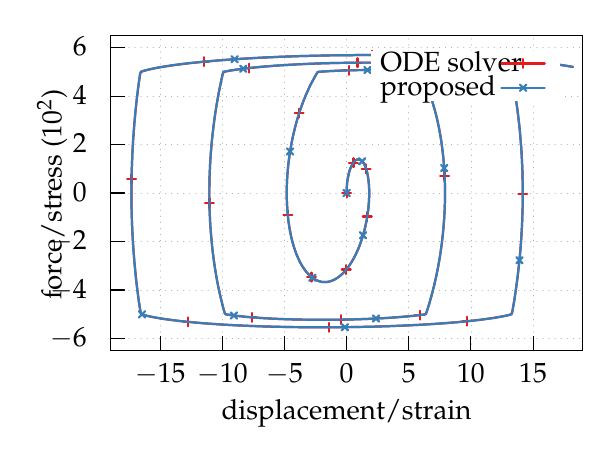
\begin{tikzpicture}[gnuplot]
%% generated with GNUPLOT 5.2p7 (Lua 5.3; terminal rev. Nov 2018, script rev. 107)
%% 09/04/2020 23:58:59
\path (0.000,0.000) rectangle (6.000,4.000);
\gpcolor{color=gp lt color axes}
\gpsetlinetype{gp lt axes}
\gpsetdashtype{gp dt axes}
\gpsetlinewidth{0.50}
\draw[gp path] (0.000,0.154)--(5.999,0.154);
\gpcolor{color=gp lt color border}
\gpsetlinetype{gp lt border}
\gpsetdashtype{gp dt solid}
\gpsetlinewidth{1.00}
\draw[gp path] (0.000,0.154)--(0.180,0.154);
\node[gp node right] at (-0.184,0.154) {$-6$};
\gpcolor{color=gp lt color axes}
\gpsetlinetype{gp lt axes}
\gpsetdashtype{gp dt axes}
\gpsetlinewidth{0.50}
\draw[gp path] (0.000,0.769)--(5.999,0.769);
\gpcolor{color=gp lt color border}
\gpsetlinetype{gp lt border}
\gpsetdashtype{gp dt solid}
\gpsetlinewidth{1.00}
\draw[gp path] (0.000,0.769)--(0.180,0.769);
\node[gp node right] at (-0.184,0.769) {$-4$};
\gpcolor{color=gp lt color axes}
\gpsetlinetype{gp lt axes}
\gpsetdashtype{gp dt axes}
\gpsetlinewidth{0.50}
\draw[gp path] (0.000,1.384)--(5.999,1.384);
\gpcolor{color=gp lt color border}
\gpsetlinetype{gp lt border}
\gpsetdashtype{gp dt solid}
\gpsetlinewidth{1.00}
\draw[gp path] (0.000,1.384)--(0.180,1.384);
\node[gp node right] at (-0.184,1.384) {$-2$};
\gpcolor{color=gp lt color axes}
\gpsetlinetype{gp lt axes}
\gpsetdashtype{gp dt axes}
\gpsetlinewidth{0.50}
\draw[gp path] (0.000,2.000)--(5.999,2.000);
\gpcolor{color=gp lt color border}
\gpsetlinetype{gp lt border}
\gpsetdashtype{gp dt solid}
\gpsetlinewidth{1.00}
\draw[gp path] (0.000,2.000)--(0.180,2.000);
\node[gp node right] at (-0.184,2.000) {$0$};
\gpcolor{color=gp lt color axes}
\gpsetlinetype{gp lt axes}
\gpsetdashtype{gp dt axes}
\gpsetlinewidth{0.50}
\draw[gp path] (0.000,2.615)--(5.999,2.615);
\gpcolor{color=gp lt color border}
\gpsetlinetype{gp lt border}
\gpsetdashtype{gp dt solid}
\gpsetlinewidth{1.00}
\draw[gp path] (0.000,2.615)--(0.180,2.615);
\node[gp node right] at (-0.184,2.615) {$2$};
\gpcolor{color=gp lt color axes}
\gpsetlinetype{gp lt axes}
\gpsetdashtype{gp dt axes}
\gpsetlinewidth{0.50}
\draw[gp path] (0.000,3.230)--(3.311,3.230);
\draw[gp path] (5.699,3.230)--(5.999,3.230);
\gpcolor{color=gp lt color border}
\gpsetlinetype{gp lt border}
\gpsetdashtype{gp dt solid}
\gpsetlinewidth{1.00}
\draw[gp path] (0.000,3.230)--(0.180,3.230);
\node[gp node right] at (-0.184,3.230) {$4$};
\gpcolor{color=gp lt color axes}
\gpsetlinetype{gp lt axes}
\gpsetdashtype{gp dt axes}
\gpsetlinewidth{0.50}
\draw[gp path] (0.000,3.845)--(5.999,3.845);
\gpcolor{color=gp lt color border}
\gpsetlinetype{gp lt border}
\gpsetdashtype{gp dt solid}
\gpsetlinewidth{1.00}
\draw[gp path] (0.000,3.845)--(0.180,3.845);
\node[gp node right] at (-0.184,3.845) {$6$};
\gpcolor{color=gp lt color axes}
\gpsetlinetype{gp lt axes}
\gpsetdashtype{gp dt axes}
\gpsetlinewidth{0.50}
\draw[gp path] (0.631,0.000)--(0.631,3.999);
\gpcolor{color=gp lt color border}
\gpsetlinetype{gp lt border}
\gpsetdashtype{gp dt solid}
\gpsetlinewidth{1.00}
\draw[gp path] (0.631,0.000)--(0.631,0.180);
\node[gp node center] at (0.631,-0.308) {$-15$};
\gpcolor{color=gp lt color axes}
\gpsetlinetype{gp lt axes}
\gpsetdashtype{gp dt axes}
\gpsetlinewidth{0.50}
\draw[gp path] (1.421,0.000)--(1.421,3.999);
\gpcolor{color=gp lt color border}
\gpsetlinetype{gp lt border}
\gpsetdashtype{gp dt solid}
\gpsetlinewidth{1.00}
\draw[gp path] (1.421,0.000)--(1.421,0.180);
\node[gp node center] at (1.421,-0.308) {$-10$};
\gpcolor{color=gp lt color axes}
\gpsetlinetype{gp lt axes}
\gpsetdashtype{gp dt axes}
\gpsetlinewidth{0.50}
\draw[gp path] (2.210,0.000)--(2.210,3.999);
\gpcolor{color=gp lt color border}
\gpsetlinetype{gp lt border}
\gpsetdashtype{gp dt solid}
\gpsetlinewidth{1.00}
\draw[gp path] (2.210,0.000)--(2.210,0.180);
\node[gp node center] at (2.210,-0.308) {$-5$};
\gpcolor{color=gp lt color axes}
\gpsetlinetype{gp lt axes}
\gpsetdashtype{gp dt axes}
\gpsetlinewidth{0.50}
\draw[gp path] (3.000,0.000)--(3.000,3.999);
\gpcolor{color=gp lt color border}
\gpsetlinetype{gp lt border}
\gpsetdashtype{gp dt solid}
\gpsetlinewidth{1.00}
\draw[gp path] (3.000,0.000)--(3.000,0.180);
\node[gp node center] at (3.000,-0.308) {$0$};
\gpcolor{color=gp lt color axes}
\gpsetlinetype{gp lt axes}
\gpsetdashtype{gp dt axes}
\gpsetlinewidth{0.50}
\draw[gp path] (3.789,0.000)--(3.789,3.183);
\draw[gp path] (3.789,3.799)--(3.789,3.999);
\gpcolor{color=gp lt color border}
\gpsetlinetype{gp lt border}
\gpsetdashtype{gp dt solid}
\gpsetlinewidth{1.00}
\draw[gp path] (3.789,0.000)--(3.789,0.180);
\node[gp node center] at (3.789,-0.308) {$5$};
\gpcolor{color=gp lt color axes}
\gpsetlinetype{gp lt axes}
\gpsetdashtype{gp dt axes}
\gpsetlinewidth{0.50}
\draw[gp path] (4.578,0.000)--(4.578,3.183);
\draw[gp path] (4.578,3.799)--(4.578,3.999);
\gpcolor{color=gp lt color border}
\gpsetlinetype{gp lt border}
\gpsetdashtype{gp dt solid}
\gpsetlinewidth{1.00}
\draw[gp path] (4.578,0.000)--(4.578,0.180);
\node[gp node center] at (4.578,-0.308) {$10$};
\gpcolor{color=gp lt color axes}
\gpsetlinetype{gp lt axes}
\gpsetdashtype{gp dt axes}
\gpsetlinewidth{0.50}
\draw[gp path] (5.368,0.000)--(5.368,3.183);
\draw[gp path] (5.368,3.799)--(5.368,3.999);
\gpcolor{color=gp lt color border}
\gpsetlinetype{gp lt border}
\gpsetdashtype{gp dt solid}
\gpsetlinewidth{1.00}
\draw[gp path] (5.368,0.000)--(5.368,0.180);
\node[gp node center] at (5.368,-0.308) {$15$};
\draw[gp path] (0.000,3.999)--(0.000,0.000)--(5.999,0.000)--(5.999,3.999)--cycle;
\node[gp node center,rotate=-270] at (-0.706,1.999) {force/stress (\num{e2})};
\node[gp node center] at (2.999,-0.769) {displacement/strain};
\gpcolor{rgb color={0.894,0.102,0.110}}
\gpsetlinewidth{2.00}
\draw[gp path] (3.000,2.000)--(3.000,2.002)--(3.000,2.006)--(3.000,2.012)--(3.000,2.018)%
  --(3.000,2.024)--(3.000,2.030)--(3.000,2.036)--(3.000,2.042)--(3.001,2.049)--(3.001,2.055)%
  --(3.001,2.061)--(3.001,2.067)--(3.002,2.073)--(3.002,2.079)--(3.003,2.085)--(3.003,2.091)%
  --(3.004,2.097)--(3.004,2.103)--(3.005,2.109)--(3.005,2.115)--(3.006,2.121)--(3.006,2.127)%
  --(3.007,2.133)--(3.008,2.139)--(3.009,2.144)--(3.009,2.150)--(3.010,2.156)--(3.011,2.162)%
  --(3.012,2.167)--(3.013,2.173)--(3.014,2.179)--(3.014,2.184)--(3.015,2.190)--(3.016,2.195)%
  --(3.017,2.201)--(3.018,2.206)--(3.020,2.211)--(3.021,2.217)--(3.022,2.222)--(3.023,2.227)%
  --(3.024,2.233)--(3.025,2.238)--(3.027,2.243)--(3.028,2.248)--(3.029,2.253)--(3.030,2.258)%
  --(3.032,2.263)--(3.033,2.268)--(3.035,2.272)--(3.036,2.277)--(3.037,2.282)--(3.039,2.287)%
  --(3.040,2.291)--(3.042,2.296)--(3.043,2.300)--(3.045,2.304)--(3.046,2.309)--(3.048,2.313)%
  --(3.050,2.317)--(3.051,2.321)--(3.053,2.325)--(3.055,2.329)--(3.056,2.333)--(3.058,2.337)%
  --(3.060,2.341)--(3.062,2.345)--(3.063,2.348)--(3.065,2.352)--(3.067,2.356)--(3.069,2.359)%
  --(3.071,2.362)--(3.073,2.366)--(3.074,2.369)--(3.076,2.372)--(3.078,2.375)--(3.080,2.378)%
  --(3.082,2.381)--(3.084,2.384)--(3.086,2.386)--(3.088,2.389)--(3.090,2.392)--(3.092,2.394)%
  --(3.094,2.396)--(3.096,2.399)--(3.098,2.401)--(3.100,2.403)--(3.102,2.405)--(3.104,2.407)%
  --(3.107,2.409)--(3.109,2.411)--(3.111,2.413)--(3.113,2.414)--(3.115,2.416)--(3.117,2.417)%
  --(3.119,2.418)--(3.121,2.420)--(3.124,2.421)--(3.126,2.422)--(3.128,2.423)--(3.130,2.424)%
  --(3.132,2.425)--(3.135,2.425)--(3.137,2.426)--(3.139,2.426)--(3.141,2.427)--(3.143,2.427)%
  --(3.145,2.427)--(3.148,2.427)--(3.150,2.427)--(3.152,2.427)--(3.154,2.427)--(3.156,2.427)%
  --(3.159,2.426)--(3.161,2.426)--(3.163,2.425)--(3.165,2.425)--(3.167,2.424)--(3.170,2.423)%
  --(3.172,2.422)--(3.174,2.421)--(3.176,2.420)--(3.178,2.419)--(3.180,2.417)--(3.183,2.416)%
  --(3.185,2.414)--(3.187,2.413)--(3.189,2.411)--(3.191,2.409)--(3.193,2.407)--(3.195,2.405)%
  --(3.197,2.403)--(3.199,2.401)--(3.201,2.398)--(3.203,2.396)--(3.205,2.393)--(3.207,2.391)%
  --(3.209,2.388)--(3.211,2.385)--(3.213,2.382)--(3.215,2.379)--(3.217,2.376)--(3.219,2.373)%
  --(3.221,2.369)--(3.223,2.366)--(3.225,2.362)--(3.227,2.359)--(3.229,2.355)--(3.230,2.351)%
  --(3.232,2.347)--(3.234,2.343)--(3.236,2.339)--(3.237,2.335)--(3.239,2.330)--(3.241,2.326)%
  --(3.242,2.322)--(3.244,2.317)--(3.246,2.312)--(3.247,2.307)--(3.249,2.303)--(3.250,2.298)%
  --(3.252,2.293)--(3.253,2.287)--(3.255,2.282)--(3.256,2.277)--(3.258,2.271)--(3.259,2.266)%
  --(3.261,2.260)--(3.262,2.255)--(3.263,2.249)--(3.264,2.243)--(3.266,2.237)--(3.267,2.231)%
  --(3.268,2.225)--(3.269,2.219)--(3.270,2.213)--(3.271,2.206)--(3.272,2.200)--(3.273,2.193)%
  --(3.274,2.187)--(3.275,2.180)--(3.276,2.173)--(3.277,2.166)--(3.278,2.159)--(3.279,2.153)%
  --(3.279,2.145)--(3.280,2.138)--(3.281,2.131)--(3.282,2.124)--(3.282,2.117)--(3.283,2.109)%
  --(3.283,2.102)--(3.284,2.094)--(3.284,2.086)--(3.285,2.079)--(3.285,2.071)--(3.285,2.063)%
  --(3.286,2.055)--(3.286,2.047)--(3.286,2.039)--(3.286,2.031)--(3.287,2.023)--(3.287,2.015)%
  --(3.287,2.007)--(3.287,1.998)--(3.287,1.990)--(3.287,1.982)--(3.287,1.973)--(3.286,1.965)%
  --(3.286,1.956)--(3.286,1.948)--(3.286,1.939)--(3.285,1.930)--(3.285,1.921)--(3.285,1.913)%
  --(3.284,1.904)--(3.284,1.895)--(3.283,1.886)--(3.282,1.877)--(3.282,1.868)--(3.281,1.859)%
  --(3.280,1.850)--(3.279,1.841)--(3.279,1.832)--(3.278,1.822)--(3.277,1.813)--(3.276,1.804)%
  --(3.275,1.795)--(3.274,1.785)--(3.273,1.776)--(3.271,1.767)--(3.270,1.757)--(3.269,1.748)%
  --(3.268,1.739)--(3.266,1.729)--(3.265,1.720)--(3.263,1.710)--(3.262,1.701)--(3.260,1.691)%
  --(3.259,1.682)--(3.257,1.672)--(3.255,1.663)--(3.254,1.653)--(3.252,1.644)--(3.250,1.634)%
  --(3.248,1.625)--(3.246,1.615)--(3.244,1.606)--(3.242,1.596)--(3.240,1.587)--(3.238,1.577)%
  --(3.236,1.567)--(3.233,1.558)--(3.231,1.548)--(3.229,1.539)--(3.226,1.529)--(3.224,1.520)%
  --(3.221,1.510)--(3.219,1.501)--(3.216,1.492)--(3.214,1.482)--(3.211,1.473)--(3.208,1.463)%
  --(3.206,1.454)--(3.203,1.445)--(3.200,1.435)--(3.197,1.426)--(3.194,1.417)--(3.191,1.408)%
  --(3.188,1.398)--(3.185,1.389)--(3.182,1.380)--(3.178,1.371)--(3.175,1.362)--(3.172,1.353)%
  --(3.169,1.344)--(3.165,1.335)--(3.162,1.326)--(3.158,1.317)--(3.155,1.308)--(3.151,1.300)%
  --(3.148,1.291)--(3.144,1.282)--(3.140,1.274)--(3.136,1.265)--(3.133,1.257)--(3.129,1.248)%
  --(3.125,1.240)--(3.121,1.232)--(3.117,1.223)--(3.113,1.215)--(3.109,1.207)--(3.105,1.199)%
  --(3.101,1.191)--(3.097,1.183)--(3.092,1.175)--(3.088,1.167)--(3.084,1.160)--(3.080,1.152)%
  --(3.075,1.144)--(3.071,1.137)--(3.066,1.129)--(3.062,1.122)--(3.057,1.115)--(3.053,1.108)%
  --(3.048,1.100)--(3.044,1.093)--(3.039,1.086)--(3.034,1.080)--(3.029,1.073)--(3.025,1.066)%
  --(3.020,1.060)--(3.015,1.053)--(3.010,1.047)--(3.005,1.040)--(3.000,1.034)--(2.995,1.028)%
  --(2.990,1.022)--(2.985,1.016)--(2.980,1.010)--(2.975,1.005)--(2.970,0.999)--(2.965,0.993)%
  --(2.960,0.988)--(2.954,0.983)--(2.949,0.977)--(2.944,0.972)--(2.939,0.967)--(2.933,0.963)%
  --(2.928,0.958)--(2.923,0.953)--(2.917,0.949)--(2.912,0.944)--(2.906,0.940)--(2.901,0.936)%
  --(2.896,0.932)--(2.890,0.928)--(2.885,0.924)--(2.879,0.920)--(2.873,0.917)--(2.868,0.913)%
  --(2.862,0.910)--(2.857,0.907)--(2.851,0.903)--(2.845,0.901)--(2.840,0.898)--(2.834,0.895)%
  --(2.828,0.892)--(2.823,0.890)--(2.817,0.888)--(2.811,0.885)--(2.806,0.883)--(2.800,0.882)%
  --(2.794,0.880)--(2.788,0.878)--(2.783,0.877)--(2.777,0.875)--(2.771,0.874)--(2.765,0.873)%
  --(2.760,0.872)--(2.754,0.871)--(2.748,0.870)--(2.742,0.870)--(2.736,0.869)--(2.731,0.869)%
  --(2.725,0.869)--(2.719,0.869)--(2.713,0.869)--(2.707,0.870)--(2.702,0.870)--(2.696,0.871)%
  --(2.690,0.871)--(2.684,0.872)--(2.678,0.873)--(2.673,0.874)--(2.667,0.876)--(2.661,0.877)%
  --(2.655,0.879)--(2.650,0.881)--(2.644,0.882)--(2.638,0.885)--(2.632,0.887)--(2.627,0.889)%
  --(2.621,0.892)--(2.615,0.894)--(2.610,0.897)--(2.604,0.900)--(2.598,0.903)--(2.593,0.906)%
  --(2.587,0.910)--(2.582,0.913)--(2.576,0.917)--(2.571,0.921)--(2.565,0.925)--(2.559,0.929)%
  --(2.554,0.933)--(2.549,0.938)--(2.543,0.943)--(2.538,0.947)--(2.532,0.952)--(2.527,0.957)%
  --(2.522,0.962)--(2.516,0.968)--(2.511,0.973)--(2.506,0.979)--(2.501,0.985)--(2.495,0.991)%
  --(2.490,0.997)--(2.485,1.003)--(2.480,1.010)--(2.475,1.016)--(2.470,1.023)--(2.465,1.030)%
  --(2.460,1.037)--(2.455,1.044)--(2.450,1.051)--(2.445,1.059)--(2.440,1.066)--(2.436,1.074)%
  --(2.431,1.082)--(2.426,1.090)--(2.422,1.098)--(2.417,1.106)--(2.412,1.115)--(2.408,1.123)%
  --(2.403,1.132)--(2.399,1.141)--(2.395,1.150)--(2.390,1.159)--(2.386,1.169)--(2.382,1.178)%
  --(2.378,1.188)--(2.373,1.197)--(2.369,1.207)--(2.365,1.217)--(2.361,1.227)--(2.357,1.238)%
  --(2.354,1.248)--(2.350,1.258)--(2.346,1.269)--(2.342,1.280)--(2.339,1.291)--(2.335,1.302)%
  --(2.331,1.313)--(2.328,1.324)--(2.324,1.336)--(2.321,1.347)--(2.318,1.359)--(2.314,1.371)%
  --(2.311,1.383)--(2.308,1.395)--(2.305,1.407)--(2.302,1.419)--(2.299,1.432)--(2.296,1.444)%
  --(2.293,1.457)--(2.291,1.470)--(2.288,1.483)--(2.285,1.496)--(2.283,1.509)--(2.280,1.522)%
  --(2.278,1.535)--(2.276,1.549)--(2.273,1.562)--(2.271,1.576)--(2.269,1.590)--(2.267,1.603)%
  --(2.265,1.617)--(2.263,1.631)--(2.261,1.645)--(2.259,1.660)--(2.258,1.674)--(2.256,1.688)%
  --(2.254,1.703)--(2.253,1.718)--(2.252,1.732)--(2.250,1.747)--(2.249,1.762)--(2.248,1.777)%
  --(2.247,1.792)--(2.246,1.807)--(2.245,1.822)--(2.244,1.838)--(2.243,1.853)--(2.242,1.868)%
  --(2.242,1.884)--(2.241,1.899)--(2.241,1.915)--(2.240,1.931)--(2.240,1.947)--(2.240,1.963)%
  --(2.240,1.978)--(2.239,1.994)--(2.240,2.010)--(2.240,2.027)--(2.240,2.043)--(2.240,2.059)%
  --(2.240,2.075)--(2.241,2.092)--(2.241,2.108)--(2.242,2.124)--(2.243,2.141)--(2.243,2.157)%
  --(2.244,2.174)--(2.245,2.191)--(2.246,2.207)--(2.247,2.224)--(2.249,2.241)--(2.250,2.257)%
  --(2.251,2.274)--(2.253,2.291)--(2.254,2.308)--(2.256,2.325)--(2.257,2.341)--(2.259,2.358)%
  --(2.261,2.375)--(2.263,2.392)--(2.265,2.409)--(2.267,2.426)--(2.270,2.443)--(2.272,2.460)%
  --(2.274,2.477)--(2.277,2.494)--(2.279,2.511)--(2.282,2.528)--(2.285,2.545)--(2.288,2.562)%
  --(2.291,2.579)--(2.294,2.596)--(2.297,2.613)--(2.300,2.630)--(2.303,2.647)--(2.307,2.664)%
  --(2.310,2.681)--(2.314,2.698)--(2.317,2.715)--(2.321,2.732)--(2.325,2.749)--(2.329,2.766)%
  --(2.333,2.783)--(2.337,2.799)--(2.341,2.816)--(2.345,2.833)--(2.349,2.849)--(2.354,2.866)%
  --(2.358,2.883)--(2.363,2.899)--(2.367,2.916)--(2.372,2.932)--(2.377,2.949)--(2.382,2.965)%
  --(2.387,2.981)--(2.392,2.998)--(2.397,3.014)--(2.402,3.030)--(2.408,3.046)--(2.413,3.062)%
  --(2.419,3.078)--(2.424,3.094)--(2.430,3.110)--(2.436,3.126)--(2.441,3.141)--(2.447,3.157)%
  --(2.453,3.172)--(2.459,3.188)--(2.466,3.203)--(2.472,3.219)--(2.478,3.234)--(2.484,3.249)%
  --(2.491,3.264)--(2.497,3.279)--(2.504,3.294)--(2.511,3.308)--(2.517,3.323)--(2.524,3.338)%
  --(2.531,3.352)--(2.538,3.366)--(2.545,3.381)--(2.552,3.395)--(2.560,3.409)--(2.567,3.423)%
  --(2.574,3.436)--(2.582,3.450)--(2.589,3.464)--(2.597,3.477)--(2.604,3.490)--(2.612,3.504)%
  --(2.620,3.517)--(2.627,3.529)--(2.635,3.535)--(2.643,3.537)--(2.651,3.539)--(2.660,3.540)%
  --(2.668,3.540)--(2.676,3.541)--(2.684,3.542)--(2.693,3.542)--(2.701,3.543)--(2.710,3.543)%
  --(2.718,3.544)--(2.727,3.544)--(2.736,3.545)--(2.744,3.546)--(2.753,3.546)--(2.762,3.547)%
  --(2.771,3.547)--(2.780,3.548)--(2.789,3.548)--(2.798,3.549)--(2.807,3.549)--(2.816,3.550)%
  --(2.825,3.550)--(2.835,3.551)--(2.844,3.551)--(2.853,3.552)--(2.863,3.552)--(2.872,3.552)%
  --(2.882,3.553)--(2.891,3.553)--(2.901,3.554)--(2.910,3.554)--(2.920,3.554)--(2.930,3.555)%
  --(2.939,3.555)--(2.949,3.556)--(2.959,3.556)--(2.969,3.556)--(2.978,3.557)--(2.988,3.557)%
  --(2.998,3.557)--(3.008,3.558)--(3.018,3.558)--(3.028,3.558)--(3.038,3.558)--(3.048,3.559)%
  --(3.058,3.559)--(3.069,3.559)--(3.079,3.559)--(3.089,3.560)--(3.099,3.560)--(3.109,3.560)%
  --(3.119,3.560)--(3.130,3.560)--(3.140,3.561)--(3.150,3.561)--(3.161,3.561)--(3.171,3.561)%
  --(3.181,3.561)--(3.192,3.561)--(3.202,3.561)--(3.212,3.562)--(3.223,3.562)--(3.233,3.562)%
  --(3.243,3.562)--(3.254,3.562)--(3.264,3.562)--(3.275,3.562)--(3.285,3.562)--(3.295,3.562)%
  --(3.306,3.562)--(3.316,3.562)--(3.326,3.562)--(3.337,3.562)--(3.347,3.562)--(3.358,3.562)%
  --(3.368,3.562)--(3.378,3.562)--(3.389,3.562)--(3.399,3.561)--(3.409,3.561)--(3.420,3.561)%
  --(3.430,3.561)--(3.440,3.561)--(3.451,3.561)--(3.461,3.561)--(3.471,3.560)--(3.481,3.560)%
  --(3.491,3.560)--(3.502,3.560)--(3.512,3.560)--(3.522,3.559)--(3.532,3.559)--(3.542,3.559)%
  --(3.552,3.559)--(3.562,3.558)--(3.572,3.558)--(3.582,3.558)--(3.592,3.557)--(3.602,3.557)%
  --(3.612,3.557)--(3.622,3.556)--(3.631,3.556)--(3.641,3.556)--(3.651,3.555)--(3.660,3.555)%
  --(3.670,3.555)--(3.680,3.554)--(3.689,3.554)--(3.699,3.553)--(3.708,3.553)--(3.718,3.552)%
  --(3.727,3.552)--(3.736,3.551)--(3.745,3.551)--(3.755,3.550)--(3.764,3.550)--(3.773,3.549)%
  --(3.782,3.549)--(3.791,3.548)--(3.800,3.548)--(3.809,3.547)--(3.817,3.547)--(3.826,3.546)%
  --(3.835,3.545)--(3.843,3.545)--(3.852,3.544)--(3.860,3.544)--(3.869,3.543)--(3.877,3.542)%
  --(3.886,3.542)--(3.894,3.541)--(3.902,3.540)--(3.910,3.540)--(3.918,3.539)--(3.926,3.538)%
  --(3.934,3.530)--(3.942,3.518)--(3.949,3.504)--(3.957,3.489)--(3.965,3.474)--(3.972,3.458)%
  --(3.980,3.442)--(3.987,3.426)--(3.994,3.410)--(4.001,3.394)--(4.008,3.377)--(4.016,3.361)%
  --(4.022,3.344)--(4.029,3.327)--(4.036,3.309)--(4.043,3.292)--(4.049,3.274)--(4.056,3.256)%
  --(4.062,3.238)--(4.069,3.220)--(4.075,3.202)--(4.081,3.183)--(4.087,3.164)--(4.093,3.145)%
  --(4.099,3.126)--(4.104,3.107)--(4.110,3.088)--(4.116,3.068)--(4.121,3.048)--(4.126,3.028)%
  --(4.132,3.008)--(4.137,2.988)--(4.142,2.968)--(4.147,2.947)--(4.151,2.926)--(4.156,2.906)%
  --(4.161,2.885)--(4.165,2.863)--(4.170,2.842)--(4.174,2.821)--(4.178,2.799)--(4.182,2.777)%
  --(4.186,2.756)--(4.190,2.733)--(4.194,2.711)--(4.197,2.689)--(4.201,2.667)--(4.204,2.644)%
  --(4.207,2.622)--(4.210,2.599)--(4.213,2.576)--(4.216,2.553)--(4.219,2.530)--(4.222,2.506)%
  --(4.224,2.483)--(4.227,2.460)--(4.229,2.436)--(4.231,2.412)--(4.233,2.389)--(4.235,2.365)%
  --(4.237,2.341)--(4.239,2.317)--(4.240,2.293)--(4.242,2.268)--(4.243,2.244)--(4.244,2.219)%
  --(4.245,2.195)--(4.246,2.170)--(4.247,2.146)--(4.248,2.121)--(4.248,2.096)--(4.249,2.071)%
  --(4.249,2.046)--(4.249,2.021)--(4.249,1.996)--(4.249,1.971)--(4.249,1.946)--(4.249,1.920)%
  --(4.248,1.895)--(4.248,1.870)--(4.247,1.844)--(4.246,1.819)--(4.245,1.793)--(4.244,1.768)%
  --(4.243,1.742)--(4.241,1.717)--(4.240,1.691)--(4.238,1.665)--(4.236,1.640)--(4.234,1.614)%
  --(4.232,1.588)--(4.230,1.562)--(4.228,1.537)--(4.225,1.511)--(4.223,1.485)--(4.220,1.459)%
  --(4.217,1.433)--(4.214,1.408)--(4.211,1.382)--(4.208,1.356)--(4.205,1.330)--(4.201,1.304)%
  --(4.197,1.279)--(4.194,1.253)--(4.190,1.227)--(4.186,1.201)--(4.182,1.176)--(4.177,1.150)%
  --(4.173,1.124)--(4.168,1.099)--(4.164,1.073)--(4.159,1.048)--(4.154,1.022)--(4.149,0.997)%
  --(4.144,0.971)--(4.138,0.946)--(4.133,0.921)--(4.127,0.895)--(4.121,0.870)--(4.116,0.845)%
  --(4.110,0.820)--(4.103,0.795)--(4.097,0.770)--(4.091,0.745)--(4.084,0.720)--(4.078,0.696)%
  --(4.071,0.671)--(4.064,0.647)--(4.057,0.622)--(4.050,0.598)--(4.043,0.573)--(4.035,0.549)%
  --(4.028,0.525)--(4.020,0.501)--(4.012,0.478)--(4.004,0.467)--(3.996,0.462)--(3.988,0.459)%
  --(3.980,0.458)--(3.971,0.456)--(3.963,0.455)--(3.954,0.454)--(3.945,0.453)--(3.936,0.452)%
  --(3.927,0.450)--(3.918,0.449)--(3.909,0.448)--(3.899,0.447)--(3.890,0.446)--(3.880,0.445)%
  --(3.870,0.444)--(3.861,0.443)--(3.851,0.442)--(3.841,0.440)--(3.830,0.439)--(3.820,0.438)%
  --(3.810,0.437)--(3.799,0.436)--(3.789,0.435)--(3.778,0.434)--(3.767,0.433)--(3.756,0.432)%
  --(3.745,0.431)--(3.734,0.430)--(3.723,0.429)--(3.712,0.428)--(3.700,0.427)--(3.689,0.426)%
  --(3.677,0.425)--(3.665,0.424)--(3.653,0.424)--(3.642,0.423)--(3.630,0.422)--(3.618,0.421)%
  --(3.605,0.420)--(3.593,0.419)--(3.581,0.418)--(3.568,0.417)--(3.556,0.417)--(3.543,0.416)%
  --(3.531,0.415)--(3.518,0.414)--(3.505,0.413)--(3.492,0.413)--(3.479,0.412)--(3.466,0.411)%
  --(3.453,0.410)--(3.440,0.410)--(3.426,0.409)--(3.413,0.408)--(3.400,0.407)--(3.386,0.407)%
  --(3.373,0.406)--(3.359,0.405)--(3.345,0.405)--(3.331,0.404)--(3.318,0.404)--(3.304,0.403)%
  --(3.290,0.402)--(3.276,0.402)--(3.262,0.401)--(3.247,0.401)--(3.233,0.400)--(3.219,0.400)%
  --(3.205,0.399)--(3.190,0.399)--(3.176,0.398)--(3.162,0.398)--(3.147,0.397)--(3.133,0.397)%
  --(3.118,0.396)--(3.103,0.396)--(3.089,0.395)--(3.074,0.395)--(3.059,0.395)--(3.045,0.394)%
  --(3.030,0.394)--(3.015,0.394)--(3.000,0.393)--(2.985,0.393)--(2.970,0.393)--(2.955,0.393)%
  --(2.940,0.392)--(2.925,0.392)--(2.910,0.392)--(2.895,0.392)--(2.880,0.391)--(2.865,0.391)%
  --(2.850,0.391)--(2.835,0.391)--(2.819,0.391)--(2.804,0.391)--(2.789,0.391)--(2.774,0.390)%
  --(2.759,0.390)--(2.744,0.390)--(2.728,0.390)--(2.713,0.390)--(2.698,0.390)--(2.683,0.390)%
  --(2.668,0.390)--(2.652,0.390)--(2.637,0.390)--(2.622,0.390)--(2.607,0.390)--(2.592,0.391)%
  --(2.576,0.391)--(2.561,0.391)--(2.546,0.391)--(2.531,0.391)--(2.516,0.391)--(2.501,0.391)%
  --(2.486,0.392)--(2.471,0.392)--(2.456,0.392)--(2.441,0.392)--(2.426,0.393)--(2.411,0.393)%
  --(2.396,0.393)--(2.381,0.393)--(2.366,0.394)--(2.351,0.394)--(2.337,0.394)--(2.322,0.395)%
  --(2.307,0.395)--(2.293,0.396)--(2.278,0.396)--(2.263,0.397)--(2.249,0.397)--(2.235,0.397)%
  --(2.220,0.398)--(2.206,0.398)--(2.191,0.399)--(2.177,0.399)--(2.163,0.400)--(2.149,0.401)%
  --(2.135,0.401)--(2.121,0.402)--(2.107,0.402)--(2.093,0.403)--(2.079,0.404)--(2.065,0.404)%
  --(2.052,0.405)--(2.038,0.406)--(2.024,0.406)--(2.011,0.407)--(1.998,0.408)--(1.984,0.408)%
  --(1.971,0.409)--(1.958,0.410)--(1.945,0.411)--(1.932,0.412)--(1.919,0.412)--(1.906,0.413)%
  --(1.893,0.414)--(1.881,0.415)--(1.868,0.416)--(1.856,0.417)--(1.843,0.418)--(1.831,0.419)%
  --(1.819,0.419)--(1.807,0.420)--(1.795,0.421)--(1.783,0.422)--(1.771,0.423)--(1.759,0.424)%
  --(1.748,0.425)--(1.736,0.426)--(1.725,0.427)--(1.714,0.428)--(1.702,0.429)--(1.691,0.431)%
  --(1.680,0.432)--(1.670,0.433)--(1.659,0.434)--(1.648,0.435)--(1.638,0.436)--(1.628,0.437)%
  --(1.617,0.438)--(1.607,0.440)--(1.597,0.441)--(1.587,0.442)--(1.578,0.443)--(1.568,0.444)%
  --(1.559,0.446)--(1.549,0.447)--(1.540,0.448)--(1.531,0.449)--(1.522,0.451)--(1.513,0.452)%
  --(1.505,0.453)--(1.496,0.455)--(1.488,0.456)--(1.479,0.457)--(1.471,0.459)--(1.463,0.460)%
  --(1.455,0.470)--(1.448,0.491)--(1.440,0.517)--(1.432,0.544)--(1.425,0.572)--(1.418,0.601)%
  --(1.411,0.629)--(1.404,0.658)--(1.397,0.688)--(1.390,0.717)--(1.384,0.747)--(1.377,0.776)%
  --(1.371,0.806)--(1.365,0.836)--(1.359,0.867)--(1.353,0.897)--(1.348,0.928)--(1.342,0.959)%
  --(1.337,0.990)--(1.332,1.021)--(1.327,1.052)--(1.322,1.084)--(1.318,1.115)--(1.313,1.147)%
  --(1.309,1.179)--(1.305,1.211)--(1.301,1.243)--(1.297,1.276)--(1.293,1.308)--(1.290,1.341)%
  --(1.287,1.373)--(1.284,1.406)--(1.281,1.439)--(1.278,1.472)--(1.275,1.505)--(1.273,1.539)%
  --(1.270,1.572)--(1.268,1.606)--(1.266,1.639)--(1.265,1.673)--(1.263,1.707)--(1.262,1.741)%
  --(1.260,1.775)--(1.259,1.809)--(1.258,1.843)--(1.258,1.877)--(1.257,1.912)--(1.257,1.946)%
  --(1.257,1.980)--(1.257,2.015)--(1.257,2.050)--(1.257,2.084)--(1.258,2.119)--(1.258,2.154)%
  --(1.259,2.188)--(1.260,2.223)--(1.262,2.258)--(1.263,2.293)--(1.265,2.328)--(1.266,2.363)%
  --(1.268,2.398)--(1.270,2.433)--(1.273,2.468)--(1.275,2.503)--(1.278,2.538)--(1.281,2.573)%
  --(1.284,2.608)--(1.287,2.643)--(1.290,2.678)--(1.294,2.713)--(1.298,2.748)--(1.302,2.783)%
  --(1.306,2.818)--(1.310,2.853)--(1.315,2.888)--(1.319,2.923)--(1.324,2.958)--(1.329,2.992)%
  --(1.334,3.027)--(1.340,3.062)--(1.345,3.097)--(1.351,3.131)--(1.357,3.166)--(1.363,3.200)%
  --(1.369,3.235)--(1.375,3.269)--(1.382,3.303)--(1.389,3.338)--(1.396,3.372)--(1.403,3.406)%
  --(1.410,3.440)--(1.418,3.474)--(1.425,3.507)--(1.433,3.527)--(1.441,3.536)--(1.450,3.540)%
  --(1.458,3.542)--(1.467,3.544)--(1.476,3.546)--(1.485,3.548)--(1.494,3.550)--(1.503,3.551)%
  --(1.513,3.553)--(1.522,3.555)--(1.532,3.556)--(1.542,3.558)--(1.553,3.559)--(1.563,3.561)%
  --(1.573,3.563)--(1.584,3.564)--(1.595,3.566)--(1.606,3.567)--(1.617,3.569)--(1.628,3.571)%
  --(1.640,3.572)--(1.651,3.574)--(1.663,3.575)--(1.675,3.577)--(1.687,3.578)--(1.699,3.580)%
  --(1.712,3.581)--(1.724,3.583)--(1.737,3.584)--(1.750,3.586)--(1.763,3.587)--(1.776,3.589)%
  --(1.789,3.590)--(1.803,3.591)--(1.816,3.593)--(1.830,3.594)--(1.844,3.596)--(1.858,3.597)%
  --(1.872,3.598)--(1.886,3.600)--(1.901,3.601)--(1.915,3.602)--(1.930,3.604)--(1.945,3.605)%
  --(1.960,3.606)--(1.975,3.607)--(1.990,3.609)--(2.005,3.610)--(2.021,3.611)--(2.036,3.612)%
  --(2.052,3.614)--(2.068,3.615)--(2.084,3.616)--(2.100,3.617)--(2.116,3.618)--(2.132,3.619)%
  --(2.149,3.621)--(2.165,3.622)--(2.182,3.623)--(2.199,3.624)--(2.215,3.625)--(2.232,3.626)%
  --(2.249,3.627)--(2.267,3.628)--(2.284,3.629)--(2.301,3.630)--(2.319,3.631)--(2.336,3.632)%
  --(2.354,3.633)--(2.372,3.634)--(2.389,3.635)--(2.407,3.635)--(2.425,3.636)--(2.443,3.637)%
  --(2.462,3.638)--(2.480,3.639)--(2.498,3.640)--(2.517,3.640)--(2.535,3.641)--(2.554,3.642)%
  --(2.572,3.643)--(2.591,3.643)--(2.610,3.644)--(2.629,3.645)--(2.648,3.645)--(2.667,3.646)%
  --(2.686,3.647)--(2.705,3.647)--(2.724,3.648)--(2.744,3.648)--(2.763,3.649)--(2.782,3.649)%
  --(2.802,3.650)--(2.821,3.650)--(2.841,3.651)--(2.860,3.651)--(2.880,3.652)--(2.899,3.652)%
  --(2.919,3.653)--(2.939,3.653)--(2.959,3.653)--(2.978,3.654)--(2.998,3.654)--(3.018,3.654)%
  --(3.038,3.655)--(3.058,3.655)--(3.078,3.655)--(3.098,3.655)--(3.118,3.655)--(3.138,3.656)%
  --(3.158,3.656)--(3.178,3.656)--(3.198,3.656)--(3.218,3.656)--(3.238,3.656)--(3.258,3.656)%
  --(3.278,3.656)--(3.298,3.656)--(3.318,3.656)--(3.338,3.656)--(3.359,3.656)--(3.379,3.656)%
  --(3.399,3.656)--(3.419,3.656)--(3.439,3.656)--(3.459,3.656)--(3.479,3.656)--(3.499,3.655)%
  --(3.519,3.655)--(3.539,3.655)--(3.559,3.655)--(3.579,3.655)--(3.598,3.654)--(3.618,3.654)%
  --(3.638,3.654)--(3.658,3.653)--(3.678,3.653)--(3.697,3.653)--(3.717,3.652)--(3.737,3.652)%
  --(3.756,3.651)--(3.776,3.651)--(3.795,3.650)--(3.815,3.650)--(3.834,3.649)--(3.853,3.649)%
  --(3.873,3.648)--(3.892,3.648)--(3.911,3.647)--(3.930,3.646)--(3.949,3.646)--(3.968,3.645)%
  --(3.987,3.644)--(4.006,3.644)--(4.024,3.643)--(4.043,3.642)--(4.062,3.642)--(4.080,3.641)%
  --(4.098,3.640)--(4.117,3.639)--(4.135,3.638)--(4.153,3.637)--(4.171,3.637)--(4.189,3.636)%
  --(4.207,3.635)--(4.225,3.634)--(4.243,3.633)--(4.260,3.632)--(4.278,3.631)--(4.295,3.630)%
  --(4.312,3.629)--(4.329,3.628)--(4.347,3.627)--(4.363,3.626)--(4.380,3.625)--(4.397,3.623)%
  --(4.414,3.622)--(4.430,3.621)--(4.446,3.620)--(4.463,3.619)--(4.479,3.618)--(4.495,3.616)%
  --(4.511,3.615)--(4.526,3.614)--(4.542,3.613)--(4.557,3.611)--(4.573,3.610)--(4.588,3.609)%
  --(4.603,3.607)--(4.618,3.606)--(4.633,3.605)--(4.647,3.603)--(4.662,3.602)--(4.676,3.600)%
  --(4.690,3.599)--(4.704,3.597)--(4.718,3.596)--(4.732,3.594)--(4.746,3.593)--(4.759,3.591)%
  --(4.772,3.590)--(4.785,3.588)--(4.798,3.587)--(4.811,3.585)--(4.824,3.584)--(4.836,3.582)%
  --(4.848,3.580)--(4.860,3.579)--(4.872,3.577)--(4.884,3.575)--(4.896,3.574)--(4.907,3.572)%
  --(4.918,3.570)--(4.929,3.569)--(4.940,3.567)--(4.951,3.565)--(4.961,3.563)--(4.972,3.562)%
  --(4.982,3.560)--(4.992,3.558)--(5.002,3.556)--(5.011,3.554)--(5.020,3.553)--(5.030,3.551)%
  --(5.039,3.549)--(5.047,3.547)--(5.056,3.545)--(5.064,3.543)--(5.073,3.541)--(5.081,3.540)%
  --(5.089,3.526)--(5.096,3.496)--(5.104,3.460)--(5.111,3.422)--(5.119,3.383)--(5.126,3.343)%
  --(5.132,3.303)--(5.139,3.263)--(5.145,3.222)--(5.151,3.182)--(5.157,3.141)--(5.163,3.100)%
  --(5.169,3.059)--(5.174,3.018)--(5.179,2.976)--(5.184,2.935)--(5.189,2.893)--(5.193,2.851)%
  --(5.198,2.809)--(5.202,2.767)--(5.205,2.725)--(5.209,2.682)--(5.212,2.640)--(5.216,2.597)%
  --(5.219,2.554)--(5.221,2.511)--(5.224,2.468)--(5.226,2.425)--(5.228,2.382)--(5.230,2.338)%
  --(5.232,2.295)--(5.233,2.251)--(5.234,2.208)--(5.235,2.164)--(5.236,2.120)--(5.236,2.076)%
  --(5.237,2.032)--(5.237,1.988)--(5.237,1.944)--(5.236,1.900)--(5.236,1.856)--(5.235,1.812)%
  --(5.234,1.767)--(5.232,1.723)--(5.231,1.679)--(5.229,1.634)--(5.227,1.590)--(5.225,1.545)%
  --(5.222,1.501)--(5.220,1.457)--(5.217,1.412)--(5.214,1.368)--(5.210,1.323)--(5.207,1.279)%
  --(5.203,1.234)--(5.199,1.190)--(5.195,1.146)--(5.190,1.101)--(5.185,1.057)--(5.180,1.013)%
  --(5.175,0.968)--(5.170,0.924)--(5.164,0.880)--(5.158,0.836)--(5.152,0.792)--(5.146,0.748)%
  --(5.139,0.704)--(5.133,0.660)--(5.126,0.616)--(5.118,0.573)--(5.111,0.529)--(5.103,0.489)%
  --(5.095,0.470)--(5.087,0.462)--(5.079,0.457)--(5.070,0.454)--(5.061,0.452)--(5.052,0.449)%
  --(5.042,0.447)--(5.033,0.445)--(5.023,0.443)--(5.013,0.441)--(5.002,0.439)--(4.992,0.436)%
  --(4.981,0.434)--(4.970,0.432)--(4.959,0.430)--(4.948,0.428)--(4.936,0.426)--(4.924,0.424)%
  --(4.912,0.422)--(4.900,0.420)--(4.888,0.418)--(4.875,0.416)--(4.862,0.414)--(4.849,0.412)%
  --(4.836,0.410)--(4.823,0.408)--(4.809,0.406)--(4.795,0.404)--(4.781,0.402)--(4.767,0.400)%
  --(4.753,0.398)--(4.738,0.396)--(4.723,0.394)--(4.708,0.392)--(4.693,0.390)--(4.678,0.388)%
  --(4.662,0.387)--(4.646,0.385)--(4.630,0.383)--(4.614,0.381)--(4.598,0.379)--(4.581,0.377)%
  --(4.565,0.376)--(4.548,0.374)--(4.531,0.372)--(4.513,0.370)--(4.496,0.369)--(4.479,0.367)%
  --(4.461,0.365)--(4.443,0.364)--(4.425,0.362)--(4.407,0.360)--(4.388,0.359)--(4.370,0.357)%
  --(4.351,0.356)--(4.332,0.354)--(4.313,0.352)--(4.294,0.351)--(4.274,0.349)--(4.255,0.348)%
  --(4.235,0.346)--(4.215,0.345)--(4.195,0.344)--(4.175,0.342)--(4.155,0.341)--(4.134,0.339)%
  --(4.114,0.338)--(4.093,0.337)--(4.072,0.335)--(4.051,0.334)--(4.030,0.333)--(4.009,0.331)%
  --(3.988,0.330)--(3.966,0.329)--(3.945,0.328)--(3.923,0.326)--(3.901,0.325)--(3.879,0.324)%
  --(3.857,0.323)--(3.835,0.322)--(3.813,0.321)--(3.790,0.320)--(3.768,0.319)--(3.745,0.318)%
  --(3.722,0.317)--(3.699,0.316)--(3.677,0.315)--(3.654,0.314)--(3.630,0.313)--(3.607,0.312)%
  --(3.584,0.311)--(3.560,0.310)--(3.537,0.309)--(3.513,0.309)--(3.490,0.308)--(3.466,0.307)%
  --(3.442,0.306)--(3.418,0.306)--(3.394,0.305)--(3.370,0.304)--(3.346,0.303)--(3.322,0.303)%
  --(3.298,0.302)--(3.274,0.302)--(3.249,0.301)--(3.225,0.301)--(3.200,0.300)--(3.176,0.300)%
  --(3.151,0.299)--(3.127,0.299)--(3.102,0.298)--(3.077,0.298)--(3.053,0.297)--(3.028,0.297)%
  --(3.003,0.297)--(2.978,0.296)--(2.954,0.296)--(2.929,0.296)--(2.904,0.296)--(2.879,0.296)%
  --(2.854,0.295)--(2.829,0.295)--(2.804,0.295)--(2.779,0.295)--(2.754,0.295)--(2.729,0.295)%
  --(2.704,0.295)--(2.679,0.295)--(2.654,0.295)--(2.629,0.295)--(2.604,0.295)--(2.579,0.295)%
  --(2.554,0.295)--(2.529,0.295)--(2.504,0.295)--(2.479,0.296)--(2.454,0.296)--(2.430,0.296)%
  --(2.405,0.296)--(2.380,0.297)--(2.355,0.297)--(2.330,0.297)--(2.306,0.298)--(2.281,0.298)%
  --(2.256,0.299)--(2.232,0.299)--(2.207,0.299)--(2.183,0.300)--(2.158,0.300)--(2.134,0.301)%
  --(2.110,0.302)--(2.085,0.302)--(2.061,0.303)--(2.037,0.303)--(2.013,0.304)--(1.989,0.305)%
  --(1.965,0.305)--(1.941,0.306)--(1.918,0.307)--(1.894,0.308)--(1.870,0.309)--(1.847,0.309)%
  --(1.823,0.310)--(1.800,0.311)--(1.777,0.312)--(1.754,0.313)--(1.731,0.314)--(1.708,0.315)%
  --(1.685,0.316)--(1.662,0.317)--(1.639,0.318)--(1.617,0.319)--(1.594,0.320)--(1.572,0.321)%
  --(1.550,0.322)--(1.528,0.324)--(1.506,0.325)--(1.484,0.326)--(1.462,0.327)--(1.441,0.328)%
  --(1.419,0.330)--(1.398,0.331)--(1.377,0.332)--(1.356,0.334)--(1.335,0.335)--(1.314,0.337)%
  --(1.294,0.338)--(1.273,0.339)--(1.253,0.341)--(1.233,0.342)--(1.213,0.344)--(1.193,0.345)%
  --(1.173,0.347)--(1.154,0.348)--(1.135,0.350)--(1.115,0.352)--(1.096,0.353)--(1.078,0.355)%
  --(1.059,0.357)--(1.040,0.358)--(1.022,0.360)--(1.004,0.362)--(0.986,0.363)--(0.968,0.365)%
  --(0.951,0.367)--(0.933,0.369)--(0.916,0.371)--(0.899,0.372)--(0.882,0.374)--(0.865,0.376)%
  --(0.849,0.378)--(0.833,0.380)--(0.817,0.382)--(0.801,0.384)--(0.785,0.386)--(0.770,0.388)%
  --(0.754,0.390)--(0.739,0.392)--(0.725,0.394)--(0.710,0.396)--(0.696,0.398)--(0.681,0.400)%
  --(0.667,0.402)--(0.654,0.404)--(0.640,0.406)--(0.627,0.409)--(0.614,0.411)--(0.601,0.413)%
  --(0.588,0.415)--(0.576,0.417)--(0.564,0.420)--(0.552,0.422)--(0.540,0.424)--(0.529,0.426)%
  --(0.517,0.429)--(0.506,0.431)--(0.496,0.433)--(0.485,0.435)--(0.475,0.438)--(0.465,0.440)%
  --(0.455,0.442)--(0.446,0.445)--(0.436,0.447)--(0.427,0.449)--(0.419,0.452)--(0.410,0.454)%
  --(0.402,0.457)--(0.394,0.459)--(0.386,0.478)--(0.378,0.517)--(0.371,0.563)--(0.363,0.611)%
  --(0.356,0.661)--(0.350,0.711)--(0.343,0.762)--(0.337,0.812)--(0.331,0.863)--(0.325,0.914)%
  --(0.320,0.966)--(0.315,1.017)--(0.310,1.069)--(0.305,1.120)--(0.301,1.172)--(0.297,1.224)%
  --(0.293,1.277)--(0.289,1.329)--(0.286,1.381)--(0.283,1.434)--(0.280,1.487)--(0.278,1.539)%
  --(0.275,1.592)--(0.273,1.645)--(0.272,1.699)--(0.270,1.752)--(0.269,1.805)--(0.268,1.858)%
  --(0.268,1.912)--(0.267,1.965)--(0.267,2.019)--(0.268,2.073)--(0.268,2.126)--(0.269,2.180)%
  --(0.270,2.234)--(0.271,2.288)--(0.273,2.342)--(0.275,2.395)--(0.277,2.449)--(0.279,2.503)%
  --(0.282,2.557)--(0.285,2.611)--(0.288,2.665)--(0.292,2.719)--(0.296,2.773)--(0.300,2.827)%
  --(0.304,2.881)--(0.309,2.935)--(0.314,2.988)--(0.319,3.042)--(0.325,3.096)--(0.330,3.150)%
  --(0.336,3.203)--(0.343,3.257)--(0.349,3.310)--(0.356,3.364)--(0.363,3.417)--(0.371,3.470)%
  --(0.378,3.513)--(0.387,3.531)--(0.395,3.539)--(0.404,3.544)--(0.413,3.547)--(0.422,3.550)%
  --(0.432,3.553)--(0.442,3.556)--(0.452,3.558)--(0.462,3.561)--(0.473,3.564)--(0.484,3.566)%
  --(0.495,3.569)--(0.506,3.572)--(0.518,3.574)--(0.530,3.577)--(0.542,3.579)--(0.554,3.582)%
  --(0.567,3.585)--(0.580,3.587)--(0.593,3.590)--(0.607,3.592)--(0.621,3.595)--(0.635,3.597)%
  --(0.649,3.600)--(0.664,3.602)--(0.678,3.605)--(0.693,3.607)--(0.709,3.610)--(0.724,3.612)%
  --(0.740,3.614)--(0.756,3.617)--(0.772,3.619)--(0.789,3.622)--(0.805,3.624)--(0.822,3.626)%
  --(0.840,3.629)--(0.857,3.631)--(0.875,3.633)--(0.893,3.635)--(0.911,3.638)--(0.929,3.640)%
  --(0.948,3.642)--(0.967,3.644)--(0.986,3.647)--(1.005,3.649)--(1.025,3.651)--(1.044,3.653)%
  --(1.064,3.655)--(1.084,3.657)--(1.105,3.659)--(1.125,3.661)--(1.146,3.664)--(1.167,3.666)%
  --(1.188,3.668)--(1.210,3.670)--(1.231,3.672)--(1.253,3.674)--(1.275,3.675)--(1.297,3.677)%
  --(1.320,3.679)--(1.342,3.681)--(1.365,3.683)--(1.388,3.685)--(1.411,3.687)--(1.435,3.688)%
  --(1.458,3.690)--(1.482,3.692)--(1.506,3.694)--(1.530,3.695)--(1.554,3.697)--(1.578,3.699)%
  --(1.603,3.700)--(1.628,3.702)--(1.653,3.704)--(1.678,3.705)--(1.703,3.707)--(1.728,3.708)%
  --(1.754,3.710)--(1.780,3.711)--(1.806,3.713)--(1.831,3.714)--(1.858,3.716)--(1.884,3.717)%
  --(1.910,3.718)--(1.937,3.720)--(1.964,3.721)--(1.990,3.722)--(2.017,3.724)--(2.044,3.725)%
  --(2.072,3.726)--(2.099,3.727)--(2.126,3.728)--(2.154,3.730)--(2.182,3.731)--(2.209,3.732)%
  --(2.237,3.733)--(2.265,3.734)--(2.294,3.735)--(2.322,3.736)--(2.350,3.737)--(2.378,3.738)%
  --(2.407,3.739)--(2.436,3.739)--(2.464,3.740)--(2.493,3.741)--(2.522,3.742)--(2.551,3.743)%
  --(2.580,3.743)--(2.609,3.744)--(2.638,3.745)--(2.667,3.745)--(2.696,3.746)--(2.726,3.747)%
  --(2.755,3.747)--(2.784,3.748)--(2.814,3.748)--(2.844,3.749)--(2.873,3.749)--(2.903,3.749)%
  --(2.932,3.750)--(2.962,3.750)--(2.992,3.751)--(3.022,3.751)--(3.051,3.751)--(3.081,3.751)%
  --(3.111,3.752)--(3.141,3.752)--(3.171,3.752)--(3.201,3.752)--(3.231,3.752)--(3.261,3.752)%
  --(3.290,3.752)--(3.320,3.752)--(3.350,3.752)--(3.380,3.752)--(3.410,3.752)--(3.440,3.752)%
  --(3.470,3.752)--(3.500,3.752)--(3.530,3.751)--(3.559,3.751)--(3.589,3.751)--(3.619,3.751)%
  --(3.649,3.750)--(3.679,3.750)--(3.708,3.750)--(3.738,3.749)--(3.767,3.749)--(3.797,3.748)%
  --(3.826,3.748)--(3.856,3.747)--(3.885,3.747)--(3.915,3.746)--(3.944,3.746)--(3.973,3.745)%
  --(4.002,3.744)--(4.031,3.744)--(4.060,3.743)--(4.089,3.742)--(4.118,3.741)--(4.147,3.740)%
  --(4.175,3.740)--(4.204,3.739)--(4.232,3.738)--(4.261,3.737)--(4.289,3.736)--(4.317,3.735)%
  --(4.345,3.734)--(4.373,3.733)--(4.401,3.732)--(4.429,3.731)--(4.456,3.730)--(4.484,3.728)%
  --(4.511,3.727)--(4.538,3.726)--(4.566,3.725)--(4.593,3.723)--(4.619,3.722)--(4.646,3.721)%
  --(4.673,3.719)--(4.699,3.718)--(4.726,3.717)--(4.752,3.715)--(4.778,3.714)--(4.804,3.712)%
  --(4.829,3.711)--(4.855,3.709)--(4.880,3.708)--(4.905,3.706)--(4.930,3.704)--(4.955,3.703)%
  --(4.980,3.701)--(5.005,3.699)--(5.029,3.698)--(5.053,3.696)--(5.077,3.694)--(5.101,3.692)%
  --(5.125,3.690)--(5.148,3.689)--(5.171,3.687)--(5.194,3.685)--(5.217,3.683)--(5.240,3.681)%
  --(5.262,3.679)--(5.284,3.677)--(5.306,3.675)--(5.328,3.673)--(5.350,3.671)--(5.371,3.669)%
  --(5.392,3.667)--(5.413,3.665)--(5.434,3.662)--(5.455,3.660)--(5.475,3.658)--(5.495,3.656)%
  --(5.515,3.653)--(5.534,3.651)--(5.554,3.649)--(5.573,3.647)--(5.592,3.644)--(5.610,3.642)%
  --(5.629,3.640)--(5.647,3.637)--(5.665,3.635)--(5.682,3.632)--(5.700,3.630)--(5.717,3.627)%
  --(5.734,3.625)--(5.750,3.622)--(5.767,3.620)--(5.783,3.617)--(5.799,3.615)--(5.814,3.612)%
  --(5.830,3.610)--(5.845,3.607)--(5.859,3.604)--(5.874,3.602);
\gpsetpointsize{4.00}
\gppoint{gp mark 1}{(3.000,2.000)}
\gppoint{gp mark 1}{(3.086,2.386)}
\gppoint{gp mark 1}{(3.247,2.307)}
\gppoint{gp mark 1}{(3.262,1.701)}
\gppoint{gp mark 1}{(2.995,1.028)}
\gppoint{gp mark 1}{(2.554,0.933)}
\gppoint{gp mark 1}{(2.253,1.718)}
\gppoint{gp mark 1}{(2.397,3.014)}
\gppoint{gp mark 1}{(3.028,3.558)}
\gppoint{gp mark 1}{(3.817,3.547)}
\gppoint{gp mark 1}{(4.244,2.219)}
\gppoint{gp mark 1}{(3.927,0.450)}
\gppoint{gp mark 1}{(2.925,0.392)}
\gppoint{gp mark 1}{(1.795,0.421)}
\gppoint{gp mark 1}{(1.258,1.877)}
\gppoint{gp mark 1}{(1.763,3.587)}
\gppoint{gp mark 1}{(3.138,3.656)}
\gppoint{gp mark 1}{(4.603,3.607)}
\gppoint{gp mark 1}{(5.237,1.988)}
\gppoint{gp mark 1}{(4.531,0.372)}
\gppoint{gp mark 1}{(2.779,0.295)}
\gppoint{gp mark 1}{(0.986,0.363)}
\gppoint{gp mark 1}{(0.269,2.180)}
\gppoint{gp mark 1}{(1.188,3.668)}
\gppoint{gp mark 1}{(3.320,3.752)}
\gppoint{gp mark 1}{(5.434,3.662)}
\gpcolor{rgb color={0.216,0.494,0.722}}
\draw[gp path] (3.000,2.000)--(3.000,2.002)--(3.000,2.006)--(3.000,2.012)--(3.000,2.018)%
  --(3.000,2.024)--(3.000,2.030)--(3.000,2.036)--(3.000,2.042)--(3.001,2.049)--(3.001,2.055)%
  --(3.001,2.061)--(3.001,2.067)--(3.002,2.073)--(3.002,2.079)--(3.003,2.085)--(3.003,2.091)%
  --(3.004,2.097)--(3.004,2.103)--(3.005,2.109)--(3.005,2.115)--(3.006,2.121)--(3.006,2.127)%
  --(3.007,2.133)--(3.008,2.139)--(3.009,2.144)--(3.009,2.150)--(3.010,2.156)--(3.011,2.162)%
  --(3.012,2.167)--(3.013,2.173)--(3.014,2.179)--(3.014,2.184)--(3.015,2.190)--(3.016,2.195)%
  --(3.017,2.201)--(3.018,2.206)--(3.020,2.211)--(3.021,2.217)--(3.022,2.222)--(3.023,2.227)%
  --(3.024,2.233)--(3.025,2.238)--(3.027,2.243)--(3.028,2.248)--(3.029,2.253)--(3.030,2.258)%
  --(3.032,2.263)--(3.033,2.268)--(3.035,2.272)--(3.036,2.277)--(3.037,2.282)--(3.039,2.287)%
  --(3.040,2.291)--(3.042,2.296)--(3.043,2.300)--(3.045,2.304)--(3.046,2.309)--(3.048,2.313)%
  --(3.050,2.317)--(3.051,2.321)--(3.053,2.325)--(3.055,2.329)--(3.056,2.333)--(3.058,2.337)%
  --(3.060,2.341)--(3.062,2.345)--(3.063,2.348)--(3.065,2.352)--(3.067,2.356)--(3.069,2.359)%
  --(3.071,2.362)--(3.073,2.366)--(3.074,2.369)--(3.076,2.372)--(3.078,2.375)--(3.080,2.378)%
  --(3.082,2.381)--(3.084,2.384)--(3.086,2.386)--(3.088,2.389)--(3.090,2.392)--(3.092,2.394)%
  --(3.094,2.396)--(3.096,2.399)--(3.098,2.401)--(3.100,2.403)--(3.102,2.405)--(3.104,2.407)%
  --(3.107,2.409)--(3.109,2.411)--(3.111,2.413)--(3.113,2.414)--(3.115,2.416)--(3.117,2.417)%
  --(3.119,2.418)--(3.121,2.420)--(3.124,2.421)--(3.126,2.422)--(3.128,2.423)--(3.130,2.424)%
  --(3.132,2.425)--(3.135,2.425)--(3.137,2.426)--(3.139,2.426)--(3.141,2.427)--(3.143,2.427)%
  --(3.145,2.427)--(3.148,2.427)--(3.150,2.427)--(3.152,2.427)--(3.154,2.427)--(3.156,2.427)%
  --(3.159,2.426)--(3.161,2.426)--(3.163,2.425)--(3.165,2.425)--(3.167,2.424)--(3.170,2.423)%
  --(3.172,2.422)--(3.174,2.421)--(3.176,2.420)--(3.178,2.419)--(3.180,2.417)--(3.183,2.416)%
  --(3.185,2.414)--(3.187,2.413)--(3.189,2.411)--(3.191,2.409)--(3.193,2.407)--(3.195,2.405)%
  --(3.197,2.403)--(3.199,2.401)--(3.201,2.398)--(3.203,2.396)--(3.205,2.393)--(3.207,2.391)%
  --(3.209,2.388)--(3.211,2.385)--(3.213,2.382)--(3.215,2.379)--(3.217,2.376)--(3.219,2.373)%
  --(3.221,2.369)--(3.223,2.366)--(3.225,2.362)--(3.227,2.359)--(3.229,2.355)--(3.230,2.351)%
  --(3.232,2.347)--(3.234,2.343)--(3.236,2.339)--(3.237,2.335)--(3.239,2.330)--(3.241,2.326)%
  --(3.242,2.322)--(3.244,2.317)--(3.246,2.312)--(3.247,2.307)--(3.249,2.303)--(3.250,2.298)%
  --(3.252,2.293)--(3.253,2.287)--(3.255,2.282)--(3.256,2.277)--(3.258,2.271)--(3.259,2.266)%
  --(3.261,2.260)--(3.262,2.255)--(3.263,2.249)--(3.264,2.243)--(3.266,2.237)--(3.267,2.231)%
  --(3.268,2.225)--(3.269,2.219)--(3.270,2.213)--(3.271,2.206)--(3.272,2.200)--(3.273,2.193)%
  --(3.274,2.187)--(3.275,2.180)--(3.276,2.173)--(3.277,2.166)--(3.278,2.160)--(3.279,2.153)%
  --(3.279,2.145)--(3.280,2.138)--(3.281,2.131)--(3.282,2.124)--(3.282,2.117)--(3.283,2.109)%
  --(3.283,2.102)--(3.284,2.094)--(3.284,2.086)--(3.285,2.079)--(3.285,2.071)--(3.285,2.063)%
  --(3.286,2.055)--(3.286,2.047)--(3.286,2.039)--(3.286,2.031)--(3.287,2.023)--(3.287,2.015)%
  --(3.287,2.007)--(3.287,1.998)--(3.287,1.990)--(3.287,1.982)--(3.287,1.973)--(3.286,1.965)%
  --(3.286,1.956)--(3.286,1.948)--(3.286,1.939)--(3.285,1.930)--(3.285,1.921)--(3.285,1.913)%
  --(3.284,1.904)--(3.284,1.895)--(3.283,1.886)--(3.282,1.877)--(3.282,1.868)--(3.281,1.859)%
  --(3.280,1.850)--(3.279,1.841)--(3.279,1.832)--(3.278,1.822)--(3.277,1.813)--(3.276,1.804)%
  --(3.275,1.795)--(3.274,1.786)--(3.273,1.776)--(3.271,1.767)--(3.270,1.757)--(3.269,1.748)%
  --(3.268,1.739)--(3.266,1.729)--(3.265,1.720)--(3.263,1.710)--(3.262,1.701)--(3.260,1.691)%
  --(3.259,1.682)--(3.257,1.672)--(3.255,1.663)--(3.254,1.653)--(3.252,1.644)--(3.250,1.634)%
  --(3.248,1.625)--(3.246,1.615)--(3.244,1.606)--(3.242,1.596)--(3.240,1.587)--(3.238,1.577)%
  --(3.236,1.567)--(3.233,1.558)--(3.231,1.548)--(3.229,1.539)--(3.226,1.529)--(3.224,1.520)%
  --(3.221,1.510)--(3.219,1.501)--(3.216,1.492)--(3.214,1.482)--(3.211,1.473)--(3.208,1.463)%
  --(3.206,1.454)--(3.203,1.445)--(3.200,1.435)--(3.197,1.426)--(3.194,1.417)--(3.191,1.408)%
  --(3.188,1.398)--(3.185,1.389)--(3.182,1.380)--(3.178,1.371)--(3.175,1.362)--(3.172,1.353)%
  --(3.169,1.344)--(3.165,1.335)--(3.162,1.326)--(3.158,1.317)--(3.155,1.308)--(3.151,1.300)%
  --(3.148,1.291)--(3.144,1.282)--(3.140,1.274)--(3.136,1.265)--(3.133,1.257)--(3.129,1.248)%
  --(3.125,1.240)--(3.121,1.232)--(3.117,1.223)--(3.113,1.215)--(3.109,1.207)--(3.105,1.199)%
  --(3.101,1.191)--(3.097,1.183)--(3.092,1.175)--(3.088,1.167)--(3.084,1.160)--(3.080,1.152)%
  --(3.075,1.144)--(3.071,1.137)--(3.066,1.129)--(3.062,1.122)--(3.057,1.115)--(3.053,1.108)%
  --(3.048,1.100)--(3.044,1.093)--(3.039,1.086)--(3.034,1.080)--(3.029,1.073)--(3.025,1.066)%
  --(3.020,1.060)--(3.015,1.053)--(3.010,1.047)--(3.005,1.040)--(3.000,1.034)--(2.995,1.028)%
  --(2.990,1.022)--(2.985,1.016)--(2.980,1.010)--(2.975,1.005)--(2.970,0.999)--(2.965,0.993)%
  --(2.960,0.988)--(2.954,0.983)--(2.949,0.977)--(2.944,0.972)--(2.939,0.967)--(2.933,0.963)%
  --(2.928,0.958)--(2.923,0.953)--(2.917,0.949)--(2.912,0.944)--(2.906,0.940)--(2.901,0.936)%
  --(2.896,0.932)--(2.890,0.928)--(2.885,0.924)--(2.879,0.920)--(2.873,0.917)--(2.868,0.913)%
  --(2.862,0.910)--(2.857,0.907)--(2.851,0.903)--(2.845,0.901)--(2.840,0.898)--(2.834,0.895)%
  --(2.828,0.892)--(2.823,0.890)--(2.817,0.888)--(2.811,0.885)--(2.806,0.883)--(2.800,0.881)%
  --(2.794,0.880)--(2.788,0.878)--(2.783,0.877)--(2.777,0.875)--(2.771,0.874)--(2.765,0.873)%
  --(2.760,0.872)--(2.754,0.871)--(2.748,0.870)--(2.742,0.870)--(2.736,0.869)--(2.731,0.869)%
  --(2.725,0.869)--(2.719,0.869)--(2.713,0.869)--(2.707,0.869)--(2.702,0.870)--(2.696,0.871)%
  --(2.690,0.871)--(2.684,0.872)--(2.678,0.873)--(2.673,0.874)--(2.667,0.876)--(2.661,0.877)%
  --(2.655,0.879)--(2.650,0.881)--(2.644,0.882)--(2.638,0.885)--(2.632,0.887)--(2.627,0.889)%
  --(2.621,0.892)--(2.615,0.894)--(2.610,0.897)--(2.604,0.900)--(2.598,0.903)--(2.593,0.906)%
  --(2.587,0.910)--(2.582,0.913)--(2.576,0.917)--(2.571,0.921)--(2.565,0.925)--(2.559,0.929)%
  --(2.554,0.933)--(2.549,0.938)--(2.543,0.943)--(2.538,0.947)--(2.532,0.952)--(2.527,0.957)%
  --(2.522,0.962)--(2.516,0.968)--(2.511,0.973)--(2.506,0.979)--(2.501,0.985)--(2.495,0.991)%
  --(2.490,0.997)--(2.485,1.003)--(2.480,1.010)--(2.475,1.016)--(2.470,1.023)--(2.465,1.030)%
  --(2.460,1.037)--(2.455,1.044)--(2.450,1.051)--(2.445,1.059)--(2.440,1.066)--(2.436,1.074)%
  --(2.431,1.082)--(2.426,1.090)--(2.422,1.098)--(2.417,1.106)--(2.412,1.115)--(2.408,1.123)%
  --(2.403,1.132)--(2.399,1.141)--(2.395,1.150)--(2.390,1.159)--(2.386,1.169)--(2.382,1.178)%
  --(2.378,1.188)--(2.373,1.197)--(2.369,1.207)--(2.365,1.217)--(2.361,1.227)--(2.357,1.238)%
  --(2.354,1.248)--(2.350,1.258)--(2.346,1.269)--(2.342,1.280)--(2.339,1.291)--(2.335,1.302)%
  --(2.331,1.313)--(2.328,1.324)--(2.324,1.336)--(2.321,1.347)--(2.318,1.359)--(2.314,1.371)%
  --(2.311,1.383)--(2.308,1.395)--(2.305,1.407)--(2.302,1.419)--(2.299,1.432)--(2.296,1.444)%
  --(2.293,1.457)--(2.291,1.470)--(2.288,1.483)--(2.285,1.496)--(2.283,1.509)--(2.280,1.522)%
  --(2.278,1.535)--(2.276,1.549)--(2.273,1.562)--(2.271,1.576)--(2.269,1.590)--(2.267,1.603)%
  --(2.265,1.617)--(2.263,1.631)--(2.261,1.645)--(2.259,1.660)--(2.258,1.674)--(2.256,1.688)%
  --(2.254,1.703)--(2.253,1.718)--(2.252,1.732)--(2.250,1.747)--(2.249,1.762)--(2.248,1.777)%
  --(2.247,1.792)--(2.246,1.807)--(2.245,1.822)--(2.244,1.838)--(2.243,1.853)--(2.242,1.868)%
  --(2.242,1.884)--(2.241,1.899)--(2.241,1.915)--(2.240,1.931)--(2.240,1.947)--(2.240,1.963)%
  --(2.240,1.978)--(2.239,1.994)--(2.240,2.010)--(2.240,2.027)--(2.240,2.043)--(2.240,2.059)%
  --(2.240,2.075)--(2.241,2.092)--(2.241,2.108)--(2.242,2.124)--(2.243,2.141)--(2.243,2.157)%
  --(2.244,2.174)--(2.245,2.191)--(2.246,2.207)--(2.247,2.224)--(2.249,2.241)--(2.250,2.257)%
  --(2.251,2.274)--(2.253,2.291)--(2.254,2.308)--(2.256,2.325)--(2.257,2.341)--(2.259,2.358)%
  --(2.261,2.375)--(2.263,2.392)--(2.265,2.409)--(2.267,2.426)--(2.270,2.443)--(2.272,2.460)%
  --(2.274,2.477)--(2.277,2.494)--(2.279,2.511)--(2.282,2.528)--(2.285,2.545)--(2.288,2.562)%
  --(2.291,2.579)--(2.294,2.596)--(2.297,2.613)--(2.300,2.630)--(2.303,2.647)--(2.307,2.664)%
  --(2.310,2.681)--(2.314,2.698)--(2.317,2.715)--(2.321,2.732)--(2.325,2.749)--(2.329,2.766)%
  --(2.333,2.783)--(2.337,2.799)--(2.341,2.816)--(2.345,2.833)--(2.349,2.849)--(2.354,2.866)%
  --(2.358,2.883)--(2.363,2.899)--(2.367,2.916)--(2.372,2.932)--(2.377,2.949)--(2.382,2.965)%
  --(2.387,2.981)--(2.392,2.998)--(2.397,3.014)--(2.402,3.030)--(2.408,3.046)--(2.413,3.062)%
  --(2.419,3.078)--(2.424,3.094)--(2.430,3.110)--(2.436,3.126)--(2.441,3.141)--(2.447,3.157)%
  --(2.453,3.172)--(2.459,3.188)--(2.466,3.203)--(2.472,3.219)--(2.478,3.234)--(2.484,3.249)%
  --(2.491,3.264)--(2.497,3.279)--(2.504,3.294)--(2.511,3.308)--(2.517,3.323)--(2.524,3.338)%
  --(2.531,3.352)--(2.538,3.366)--(2.545,3.381)--(2.552,3.395)--(2.560,3.409)--(2.567,3.423)%
  --(2.574,3.436)--(2.582,3.450)--(2.589,3.464)--(2.597,3.477)--(2.604,3.490)--(2.612,3.504)%
  --(2.620,3.517)--(2.627,3.530)--(2.635,3.538)--(2.643,3.539)--(2.651,3.540)--(2.660,3.540)%
  --(2.668,3.541)--(2.676,3.542)--(2.684,3.542)--(2.693,3.543)--(2.701,3.543)--(2.710,3.544)%
  --(2.718,3.544)--(2.727,3.545)--(2.736,3.545)--(2.744,3.546)--(2.753,3.547)--(2.762,3.547)%
  --(2.771,3.548)--(2.780,3.548)--(2.789,3.549)--(2.798,3.549)--(2.807,3.550)--(2.816,3.550)%
  --(2.825,3.551)--(2.835,3.551)--(2.844,3.551)--(2.853,3.552)--(2.863,3.552)--(2.872,3.553)%
  --(2.882,3.553)--(2.891,3.554)--(2.901,3.554)--(2.910,3.554)--(2.920,3.555)--(2.930,3.555)%
  --(2.939,3.556)--(2.949,3.556)--(2.959,3.556)--(2.969,3.557)--(2.978,3.557)--(2.988,3.557)%
  --(2.998,3.558)--(3.008,3.558)--(3.018,3.558)--(3.028,3.558)--(3.038,3.559)--(3.048,3.559)%
  --(3.058,3.559)--(3.069,3.559)--(3.079,3.560)--(3.089,3.560)--(3.099,3.560)--(3.109,3.560)%
  --(3.119,3.560)--(3.130,3.561)--(3.140,3.561)--(3.150,3.561)--(3.161,3.561)--(3.171,3.561)%
  --(3.181,3.561)--(3.192,3.561)--(3.202,3.562)--(3.212,3.562)--(3.223,3.562)--(3.233,3.562)%
  --(3.243,3.562)--(3.254,3.562)--(3.264,3.562)--(3.275,3.562)--(3.285,3.562)--(3.295,3.562)%
  --(3.306,3.562)--(3.316,3.562)--(3.326,3.562)--(3.337,3.562)--(3.347,3.562)--(3.358,3.562)%
  --(3.368,3.562)--(3.378,3.562)--(3.389,3.561)--(3.399,3.561)--(3.409,3.561)--(3.420,3.561)%
  --(3.430,3.561)--(3.440,3.561)--(3.451,3.561)--(3.461,3.561)--(3.471,3.560)--(3.481,3.560)%
  --(3.491,3.560)--(3.502,3.560)--(3.512,3.559)--(3.522,3.559)--(3.532,3.559)--(3.542,3.559)%
  --(3.552,3.558)--(3.562,3.558)--(3.572,3.558)--(3.582,3.558)--(3.592,3.557)--(3.602,3.557)%
  --(3.612,3.557)--(3.622,3.556)--(3.631,3.556)--(3.641,3.555)--(3.651,3.555)--(3.660,3.555)%
  --(3.670,3.554)--(3.680,3.554)--(3.689,3.553)--(3.699,3.553)--(3.708,3.552)--(3.718,3.552)%
  --(3.727,3.551)--(3.736,3.551)--(3.745,3.550)--(3.755,3.550)--(3.764,3.549)--(3.773,3.549)%
  --(3.782,3.548)--(3.791,3.548)--(3.800,3.547)--(3.809,3.547)--(3.817,3.546)--(3.826,3.545)%
  --(3.835,3.545)--(3.843,3.544)--(3.852,3.544)--(3.860,3.543)--(3.869,3.542)--(3.877,3.542)%
  --(3.886,3.541)--(3.894,3.540)--(3.902,3.540)--(3.910,3.539)--(3.918,3.538)--(3.926,3.537)%
  --(3.934,3.530)--(3.942,3.518)--(3.949,3.504)--(3.957,3.489)--(3.965,3.474)--(3.972,3.458)%
  --(3.980,3.442)--(3.987,3.426)--(3.994,3.410)--(4.001,3.394)--(4.008,3.377)--(4.016,3.361)%
  --(4.022,3.344)--(4.029,3.327)--(4.036,3.309)--(4.043,3.292)--(4.049,3.274)--(4.056,3.256)%
  --(4.062,3.238)--(4.069,3.220)--(4.075,3.202)--(4.081,3.183)--(4.087,3.164)--(4.093,3.145)%
  --(4.099,3.126)--(4.104,3.107)--(4.110,3.088)--(4.116,3.068)--(4.121,3.048)--(4.126,3.028)%
  --(4.132,3.008)--(4.137,2.988)--(4.142,2.968)--(4.147,2.947)--(4.151,2.926)--(4.156,2.906)%
  --(4.161,2.885)--(4.165,2.863)--(4.170,2.842)--(4.174,2.821)--(4.178,2.799)--(4.182,2.777)%
  --(4.186,2.756)--(4.190,2.734)--(4.194,2.711)--(4.197,2.689)--(4.201,2.667)--(4.204,2.644)%
  --(4.207,2.622)--(4.210,2.599)--(4.213,2.576)--(4.216,2.553)--(4.219,2.530)--(4.222,2.506)%
  --(4.224,2.483)--(4.227,2.460)--(4.229,2.436)--(4.231,2.412)--(4.233,2.389)--(4.235,2.365)%
  --(4.237,2.341)--(4.239,2.317)--(4.240,2.293)--(4.242,2.268)--(4.243,2.244)--(4.244,2.219)%
  --(4.245,2.195)--(4.246,2.170)--(4.247,2.146)--(4.248,2.121)--(4.248,2.096)--(4.249,2.071)%
  --(4.249,2.046)--(4.249,2.021)--(4.249,1.996)--(4.249,1.971)--(4.249,1.946)--(4.249,1.920)%
  --(4.248,1.895)--(4.248,1.870)--(4.247,1.844)--(4.246,1.819)--(4.245,1.793)--(4.244,1.768)%
  --(4.243,1.742)--(4.241,1.717)--(4.240,1.691)--(4.238,1.665)--(4.236,1.640)--(4.234,1.614)%
  --(4.232,1.588)--(4.230,1.562)--(4.228,1.537)--(4.225,1.511)--(4.223,1.485)--(4.220,1.459)%
  --(4.217,1.433)--(4.214,1.408)--(4.211,1.382)--(4.208,1.356)--(4.205,1.330)--(4.201,1.304)%
  --(4.197,1.279)--(4.194,1.253)--(4.190,1.227)--(4.186,1.201)--(4.182,1.176)--(4.177,1.150)%
  --(4.173,1.124)--(4.168,1.099)--(4.164,1.073)--(4.159,1.048)--(4.154,1.022)--(4.149,0.997)%
  --(4.144,0.971)--(4.138,0.946)--(4.133,0.921)--(4.127,0.895)--(4.121,0.870)--(4.116,0.845)%
  --(4.110,0.820)--(4.103,0.795)--(4.097,0.770)--(4.091,0.745)--(4.084,0.720)--(4.078,0.696)%
  --(4.071,0.671)--(4.064,0.647)--(4.057,0.622)--(4.050,0.598)--(4.043,0.573)--(4.035,0.549)%
  --(4.028,0.525)--(4.020,0.501)--(4.012,0.477)--(4.004,0.460)--(3.996,0.458)--(3.988,0.458)%
  --(3.980,0.456)--(3.971,0.455)--(3.963,0.454)--(3.954,0.453)--(3.945,0.452)--(3.936,0.451)%
  --(3.927,0.449)--(3.918,0.448)--(3.909,0.447)--(3.899,0.446)--(3.890,0.445)--(3.880,0.444)%
  --(3.870,0.443)--(3.861,0.442)--(3.851,0.441)--(3.841,0.440)--(3.830,0.439)--(3.820,0.438)%
  --(3.810,0.437)--(3.799,0.436)--(3.789,0.435)--(3.778,0.433)--(3.767,0.432)--(3.756,0.431)%
  --(3.745,0.431)--(3.734,0.430)--(3.723,0.429)--(3.712,0.428)--(3.700,0.427)--(3.689,0.426)%
  --(3.677,0.425)--(3.665,0.424)--(3.653,0.423)--(3.642,0.422)--(3.630,0.421)--(3.618,0.420)%
  --(3.605,0.419)--(3.593,0.419)--(3.581,0.418)--(3.568,0.417)--(3.556,0.416)--(3.543,0.415)%
  --(3.531,0.414)--(3.518,0.414)--(3.505,0.413)--(3.492,0.412)--(3.479,0.411)--(3.466,0.411)%
  --(3.453,0.410)--(3.440,0.409)--(3.426,0.408)--(3.413,0.408)--(3.400,0.407)--(3.386,0.406)%
  --(3.373,0.406)--(3.359,0.405)--(3.345,0.404)--(3.331,0.404)--(3.318,0.403)--(3.304,0.403)%
  --(3.290,0.402)--(3.276,0.401)--(3.262,0.401)--(3.248,0.400)--(3.233,0.400)--(3.219,0.399)%
  --(3.205,0.399)--(3.190,0.398)--(3.176,0.398)--(3.162,0.397)--(3.147,0.397)--(3.133,0.397)%
  --(3.118,0.396)--(3.103,0.396)--(3.089,0.395)--(3.074,0.395)--(3.059,0.395)--(3.045,0.394)%
  --(3.030,0.394)--(3.015,0.394)--(3.000,0.393)--(2.985,0.393)--(2.970,0.393)--(2.955,0.392)%
  --(2.940,0.392)--(2.925,0.392)--(2.910,0.392)--(2.895,0.391)--(2.880,0.391)--(2.865,0.391)%
  --(2.850,0.391)--(2.835,0.391)--(2.819,0.391)--(2.804,0.391)--(2.789,0.390)--(2.774,0.390)%
  --(2.759,0.390)--(2.744,0.390)--(2.728,0.390)--(2.713,0.390)--(2.698,0.390)--(2.683,0.390)%
  --(2.668,0.390)--(2.652,0.390)--(2.637,0.390)--(2.622,0.390)--(2.607,0.390)--(2.592,0.391)%
  --(2.576,0.391)--(2.561,0.391)--(2.546,0.391)--(2.531,0.391)--(2.516,0.391)--(2.501,0.391)%
  --(2.486,0.392)--(2.471,0.392)--(2.456,0.392)--(2.441,0.392)--(2.426,0.393)--(2.411,0.393)%
  --(2.396,0.393)--(2.381,0.394)--(2.366,0.394)--(2.351,0.394)--(2.337,0.395)--(2.322,0.395)%
  --(2.307,0.395)--(2.293,0.396)--(2.278,0.396)--(2.263,0.397)--(2.249,0.397)--(2.235,0.398)%
  --(2.220,0.398)--(2.206,0.399)--(2.191,0.399)--(2.177,0.400)--(2.163,0.400)--(2.149,0.401)%
  --(2.135,0.401)--(2.121,0.402)--(2.107,0.403)--(2.093,0.403)--(2.079,0.404)--(2.065,0.405)%
  --(2.052,0.405)--(2.038,0.406)--(2.024,0.407)--(2.011,0.407)--(1.998,0.408)--(1.984,0.409)%
  --(1.971,0.410)--(1.958,0.410)--(1.945,0.411)--(1.932,0.412)--(1.919,0.413)--(1.906,0.414)%
  --(1.893,0.415)--(1.881,0.415)--(1.868,0.416)--(1.856,0.417)--(1.843,0.418)--(1.831,0.419)%
  --(1.819,0.420)--(1.807,0.421)--(1.795,0.422)--(1.783,0.423)--(1.771,0.424)--(1.759,0.425)%
  --(1.748,0.426)--(1.736,0.427)--(1.725,0.428)--(1.714,0.429)--(1.702,0.430)--(1.691,0.431)%
  --(1.680,0.432)--(1.670,0.434)--(1.659,0.435)--(1.648,0.436)--(1.638,0.437)--(1.628,0.438)%
  --(1.617,0.439)--(1.607,0.441)--(1.597,0.442)--(1.587,0.443)--(1.578,0.444)--(1.568,0.445)%
  --(1.559,0.447)--(1.549,0.448)--(1.540,0.449)--(1.531,0.451)--(1.522,0.452)--(1.513,0.453)%
  --(1.505,0.454)--(1.496,0.456)--(1.488,0.457)--(1.479,0.458)--(1.471,0.460)--(1.463,0.461)%
  --(1.455,0.470)--(1.448,0.491)--(1.440,0.516)--(1.432,0.544)--(1.425,0.572)--(1.418,0.600)%
  --(1.411,0.629)--(1.404,0.658)--(1.397,0.688)--(1.390,0.717)--(1.384,0.747)--(1.377,0.776)%
  --(1.371,0.806)--(1.365,0.836)--(1.359,0.867)--(1.353,0.897)--(1.348,0.928)--(1.342,0.959)%
  --(1.337,0.990)--(1.332,1.021)--(1.327,1.052)--(1.322,1.084)--(1.318,1.115)--(1.313,1.147)%
  --(1.309,1.179)--(1.305,1.211)--(1.301,1.243)--(1.297,1.276)--(1.293,1.308)--(1.290,1.341)%
  --(1.287,1.373)--(1.284,1.406)--(1.281,1.439)--(1.278,1.472)--(1.275,1.505)--(1.273,1.539)%
  --(1.270,1.572)--(1.268,1.606)--(1.266,1.639)--(1.265,1.673)--(1.263,1.707)--(1.262,1.741)%
  --(1.260,1.775)--(1.259,1.809)--(1.258,1.843)--(1.258,1.877)--(1.257,1.912)--(1.257,1.946)%
  --(1.257,1.980)--(1.257,2.015)--(1.257,2.050)--(1.257,2.084)--(1.258,2.119)--(1.258,2.154)%
  --(1.259,2.188)--(1.260,2.223)--(1.262,2.258)--(1.263,2.293)--(1.265,2.328)--(1.266,2.363)%
  --(1.268,2.398)--(1.270,2.433)--(1.273,2.468)--(1.275,2.503)--(1.278,2.538)--(1.281,2.573)%
  --(1.284,2.608)--(1.287,2.643)--(1.290,2.678)--(1.294,2.713)--(1.298,2.748)--(1.302,2.783)%
  --(1.306,2.818)--(1.310,2.853)--(1.315,2.888)--(1.319,2.923)--(1.324,2.958)--(1.329,2.992)%
  --(1.334,3.027)--(1.340,3.062)--(1.345,3.097)--(1.351,3.131)--(1.357,3.166)--(1.363,3.200)%
  --(1.369,3.235)--(1.375,3.269)--(1.382,3.303)--(1.389,3.338)--(1.396,3.372)--(1.403,3.406)%
  --(1.410,3.440)--(1.418,3.474)--(1.425,3.508)--(1.433,3.538)--(1.441,3.542)--(1.450,3.542)%
  --(1.458,3.545)--(1.467,3.545)--(1.476,3.548)--(1.485,3.549)--(1.494,3.551)--(1.503,3.552)%
  --(1.513,3.554)--(1.522,3.556)--(1.532,3.558)--(1.542,3.559)--(1.553,3.561)--(1.563,3.562)%
  --(1.573,3.564)--(1.584,3.565)--(1.595,3.567)--(1.606,3.569)--(1.617,3.570)--(1.628,3.572)%
  --(1.640,3.573)--(1.651,3.575)--(1.663,3.576)--(1.675,3.578)--(1.687,3.579)--(1.699,3.581)%
  --(1.712,3.582)--(1.724,3.584)--(1.737,3.585)--(1.750,3.587)--(1.763,3.588)--(1.776,3.589)%
  --(1.789,3.591)--(1.803,3.592)--(1.816,3.594)--(1.830,3.595)--(1.844,3.596)--(1.858,3.598)%
  --(1.872,3.599)--(1.886,3.600)--(1.901,3.602)--(1.915,3.603)--(1.930,3.604)--(1.945,3.606)%
  --(1.960,3.607)--(1.975,3.608)--(1.990,3.609)--(2.005,3.611)--(2.021,3.612)--(2.036,3.613)%
  --(2.052,3.614)--(2.068,3.615)--(2.084,3.617)--(2.100,3.618)--(2.116,3.619)--(2.132,3.620)%
  --(2.149,3.621)--(2.165,3.622)--(2.182,3.623)--(2.199,3.624)--(2.215,3.625)--(2.232,3.626)%
  --(2.249,3.627)--(2.267,3.628)--(2.284,3.629)--(2.301,3.630)--(2.319,3.631)--(2.336,3.632)%
  --(2.354,3.633)--(2.372,3.634)--(2.389,3.635)--(2.407,3.636)--(2.425,3.637)--(2.443,3.637)%
  --(2.462,3.638)--(2.480,3.639)--(2.498,3.640)--(2.517,3.641)--(2.535,3.641)--(2.554,3.642)%
  --(2.572,3.643)--(2.591,3.644)--(2.610,3.644)--(2.629,3.645)--(2.648,3.646)--(2.667,3.646)%
  --(2.686,3.647)--(2.705,3.647)--(2.724,3.648)--(2.744,3.649)--(2.763,3.649)--(2.782,3.650)%
  --(2.802,3.650)--(2.821,3.651)--(2.841,3.651)--(2.860,3.651)--(2.880,3.652)--(2.899,3.652)%
  --(2.919,3.653)--(2.939,3.653)--(2.959,3.653)--(2.978,3.654)--(2.998,3.654)--(3.018,3.654)%
  --(3.038,3.655)--(3.058,3.655)--(3.078,3.655)--(3.098,3.655)--(3.118,3.656)--(3.138,3.656)%
  --(3.158,3.656)--(3.178,3.656)--(3.198,3.656)--(3.218,3.656)--(3.238,3.656)--(3.258,3.656)%
  --(3.278,3.656)--(3.298,3.656)--(3.318,3.656)--(3.338,3.656)--(3.359,3.656)--(3.379,3.656)%
  --(3.399,3.656)--(3.419,3.656)--(3.439,3.656)--(3.459,3.656)--(3.479,3.656)--(3.499,3.655)%
  --(3.519,3.655)--(3.539,3.655)--(3.559,3.655)--(3.579,3.654)--(3.598,3.654)--(3.618,3.654)%
  --(3.638,3.654)--(3.658,3.653)--(3.678,3.653)--(3.697,3.652)--(3.717,3.652)--(3.737,3.652)%
  --(3.756,3.651)--(3.776,3.651)--(3.795,3.650)--(3.815,3.650)--(3.834,3.649)--(3.853,3.649)%
  --(3.873,3.648)--(3.892,3.647)--(3.911,3.647)--(3.930,3.646)--(3.949,3.646)--(3.968,3.645)%
  --(3.987,3.644)--(4.006,3.643)--(4.024,3.643)--(4.043,3.642)--(4.062,3.641)--(4.080,3.640)%
  --(4.098,3.640)--(4.117,3.639)--(4.135,3.638)--(4.153,3.637)--(4.171,3.636)--(4.189,3.635)%
  --(4.207,3.634)--(4.225,3.633)--(4.243,3.632)--(4.260,3.632)--(4.278,3.630)--(4.295,3.629)%
  --(4.312,3.628)--(4.329,3.627)--(4.347,3.626)--(4.363,3.625)--(4.380,3.624)--(4.397,3.623)%
  --(4.414,3.622)--(4.430,3.621)--(4.446,3.619)--(4.463,3.618)--(4.479,3.617)--(4.495,3.616)%
  --(4.511,3.615)--(4.526,3.613)--(4.542,3.612)--(4.557,3.611)--(4.573,3.609)--(4.588,3.608)%
  --(4.603,3.607)--(4.618,3.605)--(4.633,3.604)--(4.647,3.602)--(4.662,3.601)--(4.676,3.600)%
  --(4.690,3.598)--(4.704,3.597)--(4.718,3.595)--(4.732,3.594)--(4.746,3.592)--(4.759,3.591)%
  --(4.772,3.589)--(4.785,3.587)--(4.798,3.586)--(4.811,3.584)--(4.824,3.583)--(4.836,3.581)%
  --(4.848,3.579)--(4.860,3.578)--(4.872,3.576)--(4.884,3.574)--(4.896,3.573)--(4.907,3.571)%
  --(4.918,3.569)--(4.929,3.567)--(4.940,3.566)--(4.951,3.564)--(4.961,3.562)--(4.972,3.560)%
  --(4.982,3.559)--(4.992,3.557)--(5.002,3.555)--(5.011,3.553)--(5.020,3.551)--(5.030,3.549)%
  --(5.039,3.547)--(5.047,3.546)--(5.056,3.544)--(5.065,3.542)--(5.073,3.540)--(5.081,3.538)%
  --(5.089,3.525)--(5.096,3.496)--(5.104,3.460)--(5.111,3.422)--(5.119,3.383)--(5.126,3.343)%
  --(5.132,3.303)--(5.139,3.263)--(5.145,3.222)--(5.151,3.182)--(5.157,3.141)--(5.163,3.100)%
  --(5.169,3.059)--(5.174,3.018)--(5.179,2.976)--(5.184,2.935)--(5.189,2.893)--(5.193,2.851)%
  --(5.198,2.809)--(5.202,2.767)--(5.205,2.725)--(5.209,2.682)--(5.212,2.640)--(5.216,2.597)%
  --(5.219,2.554)--(5.221,2.511)--(5.224,2.468)--(5.226,2.425)--(5.228,2.382)--(5.230,2.338)%
  --(5.232,2.295)--(5.233,2.251)--(5.234,2.208)--(5.235,2.164)--(5.236,2.120)--(5.236,2.076)%
  --(5.237,2.032)--(5.237,1.988)--(5.237,1.944)--(5.236,1.900)--(5.236,1.856)--(5.235,1.812)%
  --(5.234,1.767)--(5.232,1.723)--(5.231,1.679)--(5.229,1.634)--(5.227,1.590)--(5.225,1.545)%
  --(5.222,1.501)--(5.220,1.457)--(5.217,1.412)--(5.214,1.368)--(5.210,1.323)--(5.207,1.279)%
  --(5.203,1.234)--(5.199,1.190)--(5.195,1.146)--(5.190,1.101)--(5.185,1.057)--(5.180,1.013)%
  --(5.175,0.968)--(5.170,0.924)--(5.164,0.880)--(5.158,0.836)--(5.152,0.792)--(5.146,0.748)%
  --(5.139,0.704)--(5.133,0.660)--(5.126,0.616)--(5.118,0.573)--(5.111,0.529)--(5.103,0.486)%
  --(5.095,0.459)--(5.087,0.456)--(5.079,0.454)--(5.070,0.452)--(5.061,0.450)--(5.052,0.448)%
  --(5.042,0.446)--(5.033,0.443)--(5.023,0.441)--(5.013,0.439)--(5.002,0.437)--(4.992,0.435)%
  --(4.981,0.433)--(4.970,0.431)--(4.959,0.429)--(4.948,0.427)--(4.936,0.425)--(4.924,0.423)%
  --(4.912,0.421)--(4.900,0.418)--(4.888,0.416)--(4.875,0.414)--(4.862,0.412)--(4.849,0.410)%
  --(4.836,0.408)--(4.823,0.407)--(4.809,0.405)--(4.795,0.403)--(4.781,0.401)--(4.767,0.399)%
  --(4.753,0.397)--(4.738,0.395)--(4.723,0.393)--(4.708,0.391)--(4.693,0.389)--(4.678,0.387)%
  --(4.662,0.386)--(4.646,0.384)--(4.630,0.382)--(4.614,0.380)--(4.598,0.378)--(4.581,0.377)%
  --(4.565,0.375)--(4.548,0.373)--(4.531,0.371)--(4.513,0.370)--(4.496,0.368)--(4.479,0.366)%
  --(4.461,0.365)--(4.443,0.363)--(4.425,0.361)--(4.407,0.360)--(4.388,0.358)--(4.370,0.357)%
  --(4.351,0.355)--(4.332,0.353)--(4.313,0.352)--(4.294,0.350)--(4.274,0.349)--(4.255,0.347)%
  --(4.235,0.346)--(4.215,0.344)--(4.195,0.343)--(4.175,0.342)--(4.155,0.340)--(4.135,0.339)%
  --(4.114,0.337)--(4.093,0.336)--(4.072,0.335)--(4.051,0.334)--(4.030,0.332)--(4.009,0.331)%
  --(3.988,0.330)--(3.966,0.328)--(3.945,0.327)--(3.923,0.326)--(3.901,0.325)--(3.879,0.324)%
  --(3.857,0.323)--(3.835,0.322)--(3.813,0.320)--(3.790,0.319)--(3.768,0.318)--(3.745,0.317)%
  --(3.722,0.316)--(3.699,0.315)--(3.677,0.314)--(3.654,0.313)--(3.630,0.313)--(3.607,0.312)%
  --(3.584,0.311)--(3.560,0.310)--(3.537,0.309)--(3.513,0.308)--(3.490,0.307)--(3.466,0.307)%
  --(3.442,0.306)--(3.418,0.305)--(3.394,0.305)--(3.370,0.304)--(3.346,0.303)--(3.322,0.303)%
  --(3.298,0.302)--(3.274,0.301)--(3.249,0.301)--(3.225,0.300)--(3.200,0.300)--(3.176,0.299)%
  --(3.151,0.299)--(3.127,0.298)--(3.102,0.298)--(3.077,0.298)--(3.053,0.297)--(3.028,0.297)%
  --(3.003,0.297)--(2.978,0.296)--(2.954,0.296)--(2.929,0.296)--(2.904,0.296)--(2.879,0.295)%
  --(2.854,0.295)--(2.829,0.295)--(2.804,0.295)--(2.779,0.295)--(2.754,0.295)--(2.729,0.295)%
  --(2.704,0.295)--(2.679,0.295)--(2.654,0.295)--(2.629,0.295)--(2.604,0.295)--(2.579,0.295)%
  --(2.554,0.295)--(2.529,0.295)--(2.504,0.295)--(2.479,0.296)--(2.454,0.296)--(2.430,0.296)%
  --(2.405,0.296)--(2.380,0.297)--(2.355,0.297)--(2.330,0.297)--(2.306,0.298)--(2.281,0.298)%
  --(2.256,0.299)--(2.232,0.299)--(2.207,0.300)--(2.183,0.300)--(2.158,0.301)--(2.134,0.301)%
  --(2.110,0.302)--(2.085,0.302)--(2.061,0.303)--(2.037,0.304)--(2.013,0.304)--(1.989,0.305)%
  --(1.965,0.306)--(1.941,0.306)--(1.918,0.307)--(1.894,0.308)--(1.870,0.309)--(1.847,0.310)%
  --(1.823,0.311)--(1.800,0.311)--(1.777,0.312)--(1.754,0.313)--(1.731,0.314)--(1.708,0.315)%
  --(1.685,0.316)--(1.662,0.317)--(1.639,0.318)--(1.617,0.319)--(1.594,0.321)--(1.572,0.322)%
  --(1.550,0.323)--(1.528,0.324)--(1.506,0.325)--(1.484,0.326)--(1.462,0.328)--(1.441,0.329)%
  --(1.419,0.330)--(1.398,0.332)--(1.377,0.333)--(1.356,0.334)--(1.335,0.336)--(1.314,0.337)%
  --(1.294,0.338)--(1.273,0.340)--(1.253,0.341)--(1.233,0.343)--(1.213,0.344)--(1.193,0.346)%
  --(1.173,0.347)--(1.154,0.349)--(1.135,0.351)--(1.115,0.352)--(1.096,0.354)--(1.077,0.356)%
  --(1.059,0.357)--(1.040,0.359)--(1.022,0.361)--(1.004,0.362)--(0.986,0.364)--(0.968,0.366)%
  --(0.951,0.368)--(0.933,0.370)--(0.916,0.371)--(0.899,0.373)--(0.882,0.375)--(0.865,0.377)%
  --(0.849,0.379)--(0.833,0.381)--(0.817,0.383)--(0.801,0.385)--(0.785,0.387)--(0.770,0.389)%
  --(0.754,0.391)--(0.739,0.393)--(0.725,0.395)--(0.710,0.397)--(0.696,0.399)--(0.681,0.401)%
  --(0.667,0.403)--(0.654,0.406)--(0.640,0.408)--(0.627,0.410)--(0.614,0.412)--(0.601,0.414)%
  --(0.588,0.416)--(0.576,0.419)--(0.564,0.421)--(0.552,0.423)--(0.540,0.426)--(0.529,0.428)%
  --(0.517,0.430)--(0.506,0.432)--(0.496,0.435)--(0.485,0.437)--(0.475,0.439)--(0.465,0.442)%
  --(0.455,0.444)--(0.446,0.447)--(0.436,0.449)--(0.427,0.451)--(0.418,0.454)--(0.410,0.456)%
  --(0.402,0.459)--(0.394,0.461)--(0.386,0.479)--(0.378,0.516)--(0.371,0.562)--(0.363,0.611)%
  --(0.356,0.661)--(0.350,0.711)--(0.343,0.762)--(0.337,0.812)--(0.331,0.863)--(0.325,0.914)%
  --(0.320,0.966)--(0.315,1.017)--(0.310,1.069)--(0.305,1.120)--(0.301,1.172)--(0.297,1.224)%
  --(0.293,1.277)--(0.289,1.329)--(0.286,1.381)--(0.283,1.434)--(0.280,1.487)--(0.278,1.539)%
  --(0.275,1.592)--(0.273,1.645)--(0.272,1.699)--(0.270,1.752)--(0.269,1.805)--(0.268,1.858)%
  --(0.268,1.912)--(0.267,1.965)--(0.267,2.019)--(0.268,2.073)--(0.268,2.126)--(0.269,2.180)%
  --(0.270,2.234)--(0.271,2.288)--(0.273,2.342)--(0.275,2.395)--(0.277,2.449)--(0.279,2.503)%
  --(0.282,2.557)--(0.285,2.611)--(0.288,2.665)--(0.292,2.719)--(0.296,2.773)--(0.300,2.827)%
  --(0.304,2.881)--(0.309,2.935)--(0.314,2.988)--(0.319,3.042)--(0.325,3.096)--(0.330,3.150)%
  --(0.336,3.203)--(0.343,3.257)--(0.349,3.310)--(0.356,3.364)--(0.363,3.417)--(0.371,3.470)%
  --(0.378,3.523)--(0.387,3.543)--(0.395,3.544)--(0.404,3.548)--(0.413,3.549)--(0.422,3.553)%
  --(0.432,3.555)--(0.441,3.558)--(0.452,3.560)--(0.462,3.563)--(0.473,3.565)--(0.484,3.568)%
  --(0.495,3.571)--(0.506,3.573)--(0.518,3.576)--(0.530,3.579)--(0.542,3.581)--(0.554,3.584)%
  --(0.567,3.586)--(0.580,3.589)--(0.593,3.591)--(0.607,3.594)--(0.621,3.596)--(0.635,3.599)%
  --(0.649,3.601)--(0.664,3.603)--(0.678,3.606)--(0.693,3.608)--(0.709,3.611)--(0.724,3.613)%
  --(0.740,3.615)--(0.756,3.618)--(0.772,3.620)--(0.789,3.623)--(0.805,3.625)--(0.822,3.627)%
  --(0.840,3.630)--(0.857,3.632)--(0.875,3.634)--(0.893,3.636)--(0.911,3.639)--(0.929,3.641)%
  --(0.948,3.643)--(0.967,3.645)--(0.986,3.647)--(1.005,3.650)--(1.024,3.652)--(1.044,3.654)%
  --(1.064,3.656)--(1.084,3.658)--(1.105,3.660)--(1.125,3.662)--(1.146,3.664)--(1.167,3.666)%
  --(1.188,3.668)--(1.210,3.670)--(1.231,3.672)--(1.253,3.674)--(1.275,3.676)--(1.297,3.678)%
  --(1.320,3.680)--(1.342,3.682)--(1.365,3.684)--(1.388,3.685)--(1.411,3.687)--(1.435,3.689)%
  --(1.458,3.691)--(1.482,3.693)--(1.506,3.694)--(1.530,3.696)--(1.554,3.698)--(1.578,3.699)%
  --(1.603,3.701)--(1.628,3.703)--(1.653,3.704)--(1.678,3.706)--(1.703,3.707)--(1.728,3.709)%
  --(1.754,3.710)--(1.780,3.712)--(1.806,3.713)--(1.831,3.715)--(1.858,3.716)--(1.884,3.717)%
  --(1.910,3.719)--(1.937,3.720)--(1.964,3.721)--(1.990,3.723)--(2.017,3.724)--(2.044,3.725)%
  --(2.072,3.726)--(2.099,3.728)--(2.126,3.729)--(2.154,3.730)--(2.182,3.731)--(2.209,3.732)%
  --(2.237,3.733)--(2.265,3.734)--(2.294,3.735)--(2.322,3.736)--(2.350,3.737)--(2.378,3.738)%
  --(2.407,3.739)--(2.436,3.740)--(2.464,3.740)--(2.493,3.741)--(2.522,3.742)--(2.551,3.743)%
  --(2.580,3.743)--(2.609,3.744)--(2.638,3.745)--(2.667,3.745)--(2.696,3.746)--(2.726,3.747)%
  --(2.755,3.747)--(2.784,3.748)--(2.814,3.748)--(2.844,3.749)--(2.873,3.749)--(2.903,3.750)%
  --(2.932,3.750)--(2.962,3.750)--(2.992,3.751)--(3.022,3.751)--(3.051,3.751)--(3.081,3.751)%
  --(3.111,3.752)--(3.141,3.752)--(3.171,3.752)--(3.201,3.752)--(3.231,3.752)--(3.261,3.752)%
  --(3.290,3.752)--(3.320,3.752)--(3.350,3.752)--(3.380,3.752)--(3.410,3.752)--(3.440,3.752)%
  --(3.470,3.752)--(3.500,3.752)--(3.530,3.751)--(3.559,3.751)--(3.589,3.751)--(3.619,3.751)%
  --(3.649,3.750)--(3.679,3.750)--(3.708,3.750)--(3.738,3.749)--(3.767,3.749)--(3.797,3.748)%
  --(3.826,3.748)--(3.856,3.747)--(3.885,3.747)--(3.915,3.746)--(3.944,3.745)--(3.973,3.745)%
  --(4.002,3.744)--(4.031,3.743)--(4.060,3.743)--(4.089,3.742)--(4.118,3.741)--(4.147,3.740)%
  --(4.175,3.739)--(4.204,3.738)--(4.232,3.738)--(4.261,3.737)--(4.289,3.736)--(4.317,3.735)%
  --(4.345,3.734)--(4.373,3.733)--(4.401,3.731)--(4.429,3.730)--(4.456,3.729)--(4.484,3.728)%
  --(4.511,3.727)--(4.538,3.726)--(4.566,3.724)--(4.593,3.723)--(4.619,3.722)--(4.646,3.720)%
  --(4.673,3.719)--(4.699,3.718)--(4.726,3.716)--(4.752,3.715)--(4.778,3.713)--(4.804,3.712)%
  --(4.829,3.710)--(4.855,3.709)--(4.880,3.707)--(4.905,3.706)--(4.930,3.704)--(4.955,3.702)%
  --(4.980,3.701)--(5.005,3.699)--(5.029,3.697)--(5.053,3.695)--(5.077,3.694)--(5.101,3.692)%
  --(5.125,3.690)--(5.148,3.688)--(5.171,3.686)--(5.194,3.684)--(5.217,3.682)--(5.240,3.680)%
  --(5.262,3.678)--(5.284,3.676)--(5.306,3.674)--(5.328,3.672)--(5.350,3.670)--(5.371,3.668)%
  --(5.392,3.666)--(5.413,3.664)--(5.434,3.662)--(5.455,3.659)--(5.475,3.657)--(5.495,3.655)%
  --(5.515,3.653)--(5.534,3.650)--(5.554,3.648)--(5.573,3.646)--(5.592,3.643)--(5.610,3.641)%
  --(5.629,3.639)--(5.647,3.636)--(5.665,3.634)--(5.682,3.631)--(5.700,3.629)--(5.717,3.626)%
  --(5.734,3.624)--(5.750,3.621)--(5.767,3.619)--(5.783,3.616)--(5.799,3.614)--(5.814,3.611)%
  --(5.830,3.608)--(5.845,3.606)--(5.859,3.603)--(5.874,3.600);
\gppoint{gp mark 2}{(3.000,2.000)}
\gppoint{gp mark 2}{(3.197,2.403)}
\gppoint{gp mark 2}{(3.208,1.463)}
\gppoint{gp mark 2}{(2.565,0.925)}
\gppoint{gp mark 2}{(2.282,2.528)}
\gppoint{gp mark 2}{(3.264,3.562)}
\gppoint{gp mark 2}{(4.239,2.317)}
\gppoint{gp mark 2}{(3.373,0.406)}
\gppoint{gp mark 2}{(1.568,0.445)}
\gppoint{gp mark 2}{(1.687,3.579)}
\gppoint{gp mark 2}{(4.043,3.642)}
\gppoint{gp mark 2}{(5.195,1.146)}
\gppoint{gp mark 2}{(2.978,0.296)}
\gppoint{gp mark 2}{(0.402,0.459)}
\gppoint{gp mark 2}{(1.578,3.699)}
\gppoint{gp mark 2}{(5.217,3.682)}
\gpfill{color=gpbgfillcolor} (3.311,3.183)--(5.699,3.183)--(5.699,3.799)--(3.311,3.799)--cycle;
\gpcolor{color=gp lt color border}
\node[gp node left] at (3.311,3.645) {ODE solver};
\gpcolor{rgb color={0.894,0.102,0.110}}
\draw[gp path] (4.967,3.645)--(5.515,3.645);
\gppoint{gp mark 1}{(5.241,3.645)}
\gpcolor{color=gp lt color border}
\node[gp node left] at (3.311,3.337) {proposed};
\gpcolor{rgb color={0.216,0.494,0.722}}
\draw[gp path] (4.967,3.337)--(5.515,3.337);
\gppoint{gp mark 2}{(5.241,3.337)}
\gpcolor{color=gp lt color border}
\gpsetlinewidth{1.00}
\draw[gp path] (0.000,3.999)--(0.000,0.000)--(5.999,0.000)--(5.999,3.999)--cycle;
%% coordinates of the plot area
\gpdefrectangularnode{gp plot 1}{\pgfpoint{0.000cm}{0.000cm}}{\pgfpoint{5.999cm}{3.999cm}}
\end{tikzpicture}
%% gnuplot variables

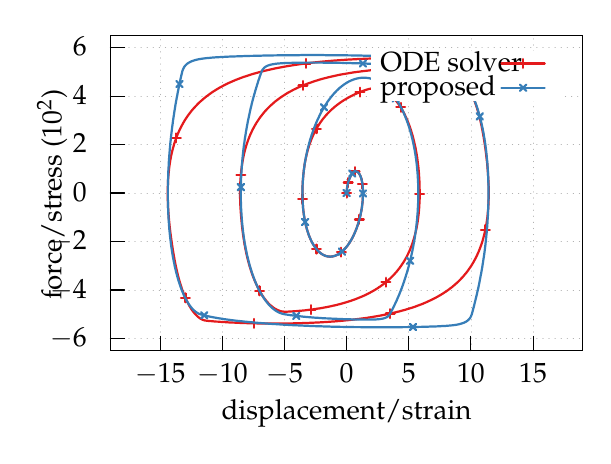
\begin{tikzpicture}[gnuplot]
%% generated with GNUPLOT 5.2p7 (Lua 5.3; terminal rev. Nov 2018, script rev. 107)
%% 09/04/2020 23:58:59
\path (0.000,0.000) rectangle (6.000,4.000);
\gpcolor{color=gp lt color axes}
\gpsetlinetype{gp lt axes}
\gpsetdashtype{gp dt axes}
\gpsetlinewidth{0.50}
\draw[gp path] (0.000,0.154)--(5.999,0.154);
\gpcolor{color=gp lt color border}
\gpsetlinetype{gp lt border}
\gpsetdashtype{gp dt solid}
\gpsetlinewidth{1.00}
\draw[gp path] (0.000,0.154)--(0.180,0.154);
\node[gp node right] at (-0.184,0.154) {$-6$};
\gpcolor{color=gp lt color axes}
\gpsetlinetype{gp lt axes}
\gpsetdashtype{gp dt axes}
\gpsetlinewidth{0.50}
\draw[gp path] (0.000,0.769)--(5.999,0.769);
\gpcolor{color=gp lt color border}
\gpsetlinetype{gp lt border}
\gpsetdashtype{gp dt solid}
\gpsetlinewidth{1.00}
\draw[gp path] (0.000,0.769)--(0.180,0.769);
\node[gp node right] at (-0.184,0.769) {$-4$};
\gpcolor{color=gp lt color axes}
\gpsetlinetype{gp lt axes}
\gpsetdashtype{gp dt axes}
\gpsetlinewidth{0.50}
\draw[gp path] (0.000,1.384)--(5.999,1.384);
\gpcolor{color=gp lt color border}
\gpsetlinetype{gp lt border}
\gpsetdashtype{gp dt solid}
\gpsetlinewidth{1.00}
\draw[gp path] (0.000,1.384)--(0.180,1.384);
\node[gp node right] at (-0.184,1.384) {$-2$};
\gpcolor{color=gp lt color axes}
\gpsetlinetype{gp lt axes}
\gpsetdashtype{gp dt axes}
\gpsetlinewidth{0.50}
\draw[gp path] (0.000,2.000)--(5.999,2.000);
\gpcolor{color=gp lt color border}
\gpsetlinetype{gp lt border}
\gpsetdashtype{gp dt solid}
\gpsetlinewidth{1.00}
\draw[gp path] (0.000,2.000)--(0.180,2.000);
\node[gp node right] at (-0.184,2.000) {$0$};
\gpcolor{color=gp lt color axes}
\gpsetlinetype{gp lt axes}
\gpsetdashtype{gp dt axes}
\gpsetlinewidth{0.50}
\draw[gp path] (0.000,2.615)--(5.999,2.615);
\gpcolor{color=gp lt color border}
\gpsetlinetype{gp lt border}
\gpsetdashtype{gp dt solid}
\gpsetlinewidth{1.00}
\draw[gp path] (0.000,2.615)--(0.180,2.615);
\node[gp node right] at (-0.184,2.615) {$2$};
\gpcolor{color=gp lt color axes}
\gpsetlinetype{gp lt axes}
\gpsetdashtype{gp dt axes}
\gpsetlinewidth{0.50}
\draw[gp path] (0.000,3.230)--(3.311,3.230);
\draw[gp path] (5.699,3.230)--(5.999,3.230);
\gpcolor{color=gp lt color border}
\gpsetlinetype{gp lt border}
\gpsetdashtype{gp dt solid}
\gpsetlinewidth{1.00}
\draw[gp path] (0.000,3.230)--(0.180,3.230);
\node[gp node right] at (-0.184,3.230) {$4$};
\gpcolor{color=gp lt color axes}
\gpsetlinetype{gp lt axes}
\gpsetdashtype{gp dt axes}
\gpsetlinewidth{0.50}
\draw[gp path] (0.000,3.845)--(5.999,3.845);
\gpcolor{color=gp lt color border}
\gpsetlinetype{gp lt border}
\gpsetdashtype{gp dt solid}
\gpsetlinewidth{1.00}
\draw[gp path] (0.000,3.845)--(0.180,3.845);
\node[gp node right] at (-0.184,3.845) {$6$};
\gpcolor{color=gp lt color axes}
\gpsetlinetype{gp lt axes}
\gpsetdashtype{gp dt axes}
\gpsetlinewidth{0.50}
\draw[gp path] (0.631,0.000)--(0.631,3.999);
\gpcolor{color=gp lt color border}
\gpsetlinetype{gp lt border}
\gpsetdashtype{gp dt solid}
\gpsetlinewidth{1.00}
\draw[gp path] (0.631,0.000)--(0.631,0.180);
\node[gp node center] at (0.631,-0.308) {$-15$};
\gpcolor{color=gp lt color axes}
\gpsetlinetype{gp lt axes}
\gpsetdashtype{gp dt axes}
\gpsetlinewidth{0.50}
\draw[gp path] (1.421,0.000)--(1.421,3.999);
\gpcolor{color=gp lt color border}
\gpsetlinetype{gp lt border}
\gpsetdashtype{gp dt solid}
\gpsetlinewidth{1.00}
\draw[gp path] (1.421,0.000)--(1.421,0.180);
\node[gp node center] at (1.421,-0.308) {$-10$};
\gpcolor{color=gp lt color axes}
\gpsetlinetype{gp lt axes}
\gpsetdashtype{gp dt axes}
\gpsetlinewidth{0.50}
\draw[gp path] (2.210,0.000)--(2.210,3.999);
\gpcolor{color=gp lt color border}
\gpsetlinetype{gp lt border}
\gpsetdashtype{gp dt solid}
\gpsetlinewidth{1.00}
\draw[gp path] (2.210,0.000)--(2.210,0.180);
\node[gp node center] at (2.210,-0.308) {$-5$};
\gpcolor{color=gp lt color axes}
\gpsetlinetype{gp lt axes}
\gpsetdashtype{gp dt axes}
\gpsetlinewidth{0.50}
\draw[gp path] (3.000,0.000)--(3.000,3.999);
\gpcolor{color=gp lt color border}
\gpsetlinetype{gp lt border}
\gpsetdashtype{gp dt solid}
\gpsetlinewidth{1.00}
\draw[gp path] (3.000,0.000)--(3.000,0.180);
\node[gp node center] at (3.000,-0.308) {$0$};
\gpcolor{color=gp lt color axes}
\gpsetlinetype{gp lt axes}
\gpsetdashtype{gp dt axes}
\gpsetlinewidth{0.50}
\draw[gp path] (3.789,0.000)--(3.789,3.183);
\draw[gp path] (3.789,3.799)--(3.789,3.999);
\gpcolor{color=gp lt color border}
\gpsetlinetype{gp lt border}
\gpsetdashtype{gp dt solid}
\gpsetlinewidth{1.00}
\draw[gp path] (3.789,0.000)--(3.789,0.180);
\node[gp node center] at (3.789,-0.308) {$5$};
\gpcolor{color=gp lt color axes}
\gpsetlinetype{gp lt axes}
\gpsetdashtype{gp dt axes}
\gpsetlinewidth{0.50}
\draw[gp path] (4.578,0.000)--(4.578,3.183);
\draw[gp path] (4.578,3.799)--(4.578,3.999);
\gpcolor{color=gp lt color border}
\gpsetlinetype{gp lt border}
\gpsetdashtype{gp dt solid}
\gpsetlinewidth{1.00}
\draw[gp path] (4.578,0.000)--(4.578,0.180);
\node[gp node center] at (4.578,-0.308) {$10$};
\gpcolor{color=gp lt color axes}
\gpsetlinetype{gp lt axes}
\gpsetdashtype{gp dt axes}
\gpsetlinewidth{0.50}
\draw[gp path] (5.368,0.000)--(5.368,3.183);
\draw[gp path] (5.368,3.799)--(5.368,3.999);
\gpcolor{color=gp lt color border}
\gpsetlinetype{gp lt border}
\gpsetdashtype{gp dt solid}
\gpsetlinewidth{1.00}
\draw[gp path] (5.368,0.000)--(5.368,0.180);
\node[gp node center] at (5.368,-0.308) {$15$};
\draw[gp path] (0.000,3.999)--(0.000,0.000)--(5.999,0.000)--(5.999,3.999)--cycle;
\node[gp node center,rotate=-270] at (-0.706,1.999) {force/stress (\num{e2})};
\node[gp node center] at (2.999,-0.769) {displacement/strain};
\gpcolor{rgb color={0.894,0.102,0.110}}
\gpsetlinewidth{2.00}
\draw[gp path] (3.000,2.000)--(3.000,2.001)--(3.000,2.002)--(3.000,2.003)--(3.000,2.004)%
  --(3.000,2.005)--(3.000,2.006)--(3.000,2.007)--(3.000,2.008)--(3.000,2.009)--(3.000,2.010)%
  --(3.000,2.011)--(3.000,2.012)--(3.000,2.013)--(3.000,2.014)--(3.000,2.016)--(3.000,2.017)%
  --(3.000,2.018)--(3.000,2.020)--(3.001,2.021)--(3.001,2.023)--(3.001,2.024)--(3.001,2.026)%
  --(3.001,2.027)--(3.001,2.029)--(3.001,2.031)--(3.002,2.032)--(3.002,2.034)--(3.002,2.036)%
  --(3.002,2.038)--(3.002,2.040)--(3.003,2.042)--(3.003,2.043)--(3.003,2.045)--(3.003,2.047)%
  --(3.003,2.049)--(3.004,2.052)--(3.004,2.054)--(3.004,2.056)--(3.005,2.058)--(3.005,2.060)%
  --(3.005,2.062)--(3.006,2.064)--(3.006,2.067)--(3.006,2.069)--(3.007,2.071)--(3.007,2.073)%
  --(3.007,2.076)--(3.008,2.078)--(3.008,2.080)--(3.009,2.083)--(3.009,2.085)--(3.009,2.088)%
  --(3.010,2.090)--(3.010,2.093)--(3.011,2.095)--(3.011,2.097)--(3.012,2.100)--(3.012,2.102)%
  --(3.013,2.105)--(3.013,2.107)--(3.014,2.110)--(3.015,2.112)--(3.015,2.115)--(3.016,2.118)%
  --(3.016,2.120)--(3.017,2.123)--(3.018,2.125)--(3.018,2.128)--(3.019,2.130)--(3.020,2.133)%
  --(3.020,2.135)--(3.021,2.138)--(3.022,2.141)--(3.022,2.143)--(3.023,2.146)--(3.024,2.148)%
  --(3.025,2.151)--(3.026,2.153)--(3.026,2.156)--(3.027,2.158)--(3.028,2.161)--(3.029,2.163)%
  --(3.030,2.166)--(3.031,2.168)--(3.031,2.171)--(3.032,2.173)--(3.033,2.176)--(3.034,2.178)%
  --(3.035,2.181)--(3.036,2.183)--(3.037,2.186)--(3.038,2.188)--(3.039,2.190)--(3.040,2.193)%
  --(3.041,2.195)--(3.042,2.197)--(3.043,2.200)--(3.044,2.202)--(3.045,2.204)--(3.046,2.206)%
  --(3.047,2.208)--(3.048,2.211)--(3.049,2.213)--(3.050,2.215)--(3.051,2.217)--(3.053,2.219)%
  --(3.054,2.221)--(3.055,2.223)--(3.056,2.225)--(3.057,2.227)--(3.058,2.229)--(3.059,2.231)%
  --(3.061,2.233)--(3.062,2.235)--(3.063,2.236)--(3.064,2.238)--(3.066,2.240)--(3.067,2.242)%
  --(3.068,2.243)--(3.069,2.245)--(3.071,2.246)--(3.072,2.248)--(3.073,2.249)--(3.074,2.251)%
  --(3.076,2.252)--(3.077,2.254)--(3.078,2.255)--(3.080,2.256)--(3.081,2.258)--(3.082,2.259)%
  --(3.084,2.260)--(3.085,2.261)--(3.086,2.262)--(3.088,2.263)--(3.089,2.264)--(3.090,2.265)%
  --(3.092,2.266)--(3.093,2.267)--(3.094,2.268)--(3.096,2.269)--(3.097,2.269)--(3.099,2.270)%
  --(3.100,2.271)--(3.101,2.271)--(3.103,2.272)--(3.104,2.272)--(3.106,2.273)--(3.107,2.273)%
  --(3.108,2.273)--(3.110,2.274)--(3.111,2.274)--(3.113,2.274)--(3.114,2.274)--(3.115,2.274)%
  --(3.117,2.274)--(3.118,2.274)--(3.120,2.274)--(3.121,2.274)--(3.122,2.274)--(3.124,2.273)%
  --(3.125,2.273)--(3.127,2.273)--(3.128,2.272)--(3.129,2.272)--(3.131,2.271)--(3.132,2.271)%
  --(3.134,2.270)--(3.135,2.269)--(3.136,2.268)--(3.138,2.267)--(3.139,2.267)--(3.141,2.266)%
  --(3.142,2.265)--(3.143,2.264)--(3.145,2.262)--(3.146,2.261)--(3.147,2.260)--(3.149,2.259)%
  --(3.150,2.257)--(3.151,2.256)--(3.153,2.254)--(3.154,2.253)--(3.155,2.251)--(3.156,2.249)%
  --(3.158,2.248)--(3.159,2.246)--(3.160,2.244)--(3.162,2.242)--(3.163,2.240)--(3.164,2.238)%
  --(3.165,2.236)--(3.166,2.234)--(3.168,2.232)--(3.169,2.229)--(3.170,2.227)--(3.171,2.225)%
  --(3.172,2.222)--(3.173,2.220)--(3.175,2.217)--(3.176,2.214)--(3.177,2.212)--(3.178,2.209)%
  --(3.179,2.206)--(3.180,2.203)--(3.181,2.200)--(3.182,2.197)--(3.183,2.194)--(3.184,2.191)%
  --(3.185,2.188)--(3.186,2.185)--(3.187,2.181)--(3.188,2.178)--(3.189,2.175)--(3.190,2.171)%
  --(3.190,2.168)--(3.191,2.164)--(3.192,2.161)--(3.193,2.157)--(3.194,2.153)--(3.195,2.149)%
  --(3.195,2.145)--(3.196,2.142)--(3.197,2.138)--(3.197,2.134)--(3.198,2.130)--(3.199,2.125)%
  --(3.199,2.121)--(3.200,2.117)--(3.201,2.113)--(3.201,2.108)--(3.202,2.104)--(3.202,2.100)%
  --(3.203,2.095)--(3.203,2.091)--(3.204,2.086)--(3.204,2.081)--(3.205,2.077)--(3.205,2.072)%
  --(3.205,2.067)--(3.206,2.062)--(3.206,2.057)--(3.206,2.052)--(3.207,2.048)--(3.207,2.043)%
  --(3.207,2.037)--(3.207,2.032)--(3.207,2.027)--(3.207,2.022)--(3.208,2.017)--(3.208,2.012)%
  --(3.208,2.006)--(3.208,2.001)--(3.208,1.995)--(3.208,1.990)--(3.208,1.985)--(3.207,1.979)%
  --(3.207,1.973)--(3.207,1.968)--(3.207,1.962)--(3.207,1.957)--(3.207,1.951)--(3.206,1.945)%
  --(3.206,1.939)--(3.206,1.934)--(3.205,1.928)--(3.205,1.922)--(3.205,1.916)--(3.204,1.910)%
  --(3.204,1.904)--(3.203,1.898)--(3.203,1.892)--(3.202,1.886)--(3.201,1.880)--(3.201,1.874)%
  --(3.200,1.868)--(3.199,1.862)--(3.199,1.856)--(3.198,1.850)--(3.197,1.843)--(3.196,1.837)%
  --(3.196,1.831)--(3.195,1.825)--(3.194,1.818)--(3.193,1.812)--(3.192,1.806)--(3.191,1.800)%
  --(3.190,1.793)--(3.189,1.787)--(3.188,1.780)--(3.186,1.774)--(3.185,1.768)--(3.184,1.761)%
  --(3.183,1.755)--(3.182,1.749)--(3.180,1.742)--(3.179,1.736)--(3.178,1.729)--(3.176,1.723)%
  --(3.175,1.716)--(3.173,1.710)--(3.172,1.704)--(3.170,1.697)--(3.169,1.691)--(3.167,1.684)%
  --(3.165,1.678)--(3.164,1.671)--(3.162,1.665)--(3.160,1.658)--(3.159,1.652)--(3.157,1.646)%
  --(3.155,1.639)--(3.153,1.633)--(3.151,1.626)--(3.149,1.620)--(3.147,1.614)--(3.145,1.607)%
  --(3.143,1.601)--(3.141,1.595)--(3.139,1.588)--(3.137,1.582)--(3.135,1.576)--(3.133,1.570)%
  --(3.130,1.563)--(3.128,1.557)--(3.126,1.551)--(3.124,1.545)--(3.121,1.539)--(3.119,1.532)%
  --(3.116,1.526)--(3.114,1.520)--(3.111,1.514)--(3.109,1.508)--(3.106,1.502)--(3.104,1.496)%
  --(3.101,1.490)--(3.099,1.484)--(3.096,1.478)--(3.093,1.473)--(3.091,1.467)--(3.088,1.461)%
  --(3.085,1.455)--(3.082,1.450)--(3.079,1.444)--(3.076,1.438)--(3.074,1.433)--(3.071,1.427)%
  --(3.068,1.422)--(3.065,1.416)--(3.062,1.411)--(3.059,1.405)--(3.056,1.400)--(3.053,1.395)%
  --(3.049,1.390)--(3.046,1.384)--(3.043,1.379)--(3.040,1.374)--(3.037,1.369)--(3.033,1.364)%
  --(3.030,1.359)--(3.027,1.354)--(3.024,1.350)--(3.020,1.345)--(3.017,1.340)--(3.013,1.335)%
  --(3.010,1.331)--(3.007,1.326)--(3.003,1.322)--(3.000,1.318)--(2.996,1.313)--(2.993,1.309)%
  --(2.989,1.305)--(2.985,1.301)--(2.982,1.296)--(2.978,1.292)--(2.975,1.288)--(2.971,1.285)%
  --(2.967,1.281)--(2.964,1.277)--(2.960,1.273)--(2.956,1.270)--(2.952,1.266)--(2.949,1.263)%
  --(2.945,1.259)--(2.941,1.256)--(2.937,1.253)--(2.933,1.250)--(2.929,1.247)--(2.926,1.244)%
  --(2.922,1.241)--(2.918,1.238)--(2.914,1.235)--(2.910,1.232)--(2.906,1.230)--(2.902,1.227)%
  --(2.898,1.225)--(2.894,1.222)--(2.890,1.220)--(2.886,1.218)--(2.882,1.216)--(2.878,1.214)%
  --(2.874,1.212)--(2.870,1.210)--(2.866,1.208)--(2.862,1.207)--(2.858,1.205)--(2.854,1.204)%
  --(2.850,1.202)--(2.846,1.201)--(2.841,1.200)--(2.837,1.199)--(2.833,1.197)--(2.829,1.197)%
  --(2.825,1.196)--(2.821,1.195)--(2.817,1.194)--(2.813,1.194)--(2.808,1.193)--(2.804,1.193)%
  --(2.800,1.193)--(2.796,1.192)--(2.792,1.192)--(2.788,1.192)--(2.784,1.192)--(2.779,1.193)%
  --(2.775,1.193)--(2.771,1.193)--(2.767,1.194)--(2.763,1.194)--(2.759,1.195)--(2.755,1.196)%
  --(2.751,1.197)--(2.746,1.198)--(2.742,1.199)--(2.738,1.200)--(2.734,1.201)--(2.730,1.203)%
  --(2.726,1.204)--(2.722,1.206)--(2.718,1.207)--(2.714,1.209)--(2.710,1.211)--(2.706,1.213)%
  --(2.702,1.215)--(2.698,1.217)--(2.694,1.220)--(2.690,1.222)--(2.686,1.225)--(2.682,1.227)%
  --(2.678,1.230)--(2.674,1.233)--(2.670,1.236)--(2.666,1.239)--(2.662,1.242)--(2.658,1.245)%
  --(2.654,1.249)--(2.650,1.252)--(2.647,1.256)--(2.643,1.259)--(2.639,1.263)--(2.635,1.267)%
  --(2.631,1.271)--(2.628,1.275)--(2.624,1.279)--(2.620,1.284)--(2.617,1.288)--(2.613,1.292)%
  --(2.609,1.297)--(2.606,1.302)--(2.602,1.307)--(2.599,1.311)--(2.595,1.316)--(2.592,1.322)%
  --(2.588,1.327)--(2.585,1.332)--(2.581,1.338)--(2.578,1.343)--(2.575,1.349)--(2.571,1.354)%
  --(2.568,1.360)--(2.565,1.366)--(2.562,1.372)--(2.558,1.378)--(2.555,1.384)--(2.552,1.391)%
  --(2.549,1.397)--(2.546,1.404)--(2.543,1.410)--(2.540,1.417)--(2.537,1.424)--(2.534,1.431)%
  --(2.531,1.438)--(2.528,1.445)--(2.525,1.452)--(2.522,1.459)--(2.520,1.466)--(2.517,1.474)%
  --(2.514,1.481)--(2.512,1.489)--(2.509,1.497)--(2.507,1.505)--(2.504,1.513)--(2.502,1.521)%
  --(2.499,1.529)--(2.497,1.537)--(2.494,1.545)--(2.492,1.553)--(2.490,1.562)--(2.488,1.570)%
  --(2.485,1.579)--(2.483,1.588)--(2.481,1.596)--(2.479,1.605)--(2.477,1.614)--(2.475,1.623)%
  --(2.473,1.632)--(2.471,1.641)--(2.470,1.651)--(2.468,1.660)--(2.466,1.669)--(2.464,1.679)%
  --(2.463,1.688)--(2.461,1.698)--(2.460,1.708)--(2.458,1.718)--(2.457,1.727)--(2.455,1.737)%
  --(2.454,1.747)--(2.453,1.757)--(2.452,1.767)--(2.450,1.778)--(2.449,1.788)--(2.448,1.798)%
  --(2.447,1.809)--(2.446,1.819)--(2.445,1.830)--(2.445,1.840)--(2.444,1.851)--(2.443,1.861)%
  --(2.442,1.872)--(2.442,1.883)--(2.441,1.894)--(2.441,1.905)--(2.440,1.916)--(2.440,1.927)%
  --(2.439,1.938)--(2.439,1.949)--(2.439,1.960)--(2.439,1.971)--(2.439,1.982)--(2.439,1.994)%
  --(2.439,2.005)--(2.439,2.016)--(2.439,2.028)--(2.439,2.039)--(2.439,2.051)--(2.439,2.062)%
  --(2.440,2.074)--(2.440,2.086)--(2.441,2.097)--(2.441,2.109)--(2.442,2.121)--(2.442,2.132)%
  --(2.443,2.144)--(2.444,2.156)--(2.445,2.168)--(2.446,2.180)--(2.447,2.192)--(2.448,2.203)%
  --(2.449,2.215)--(2.450,2.227)--(2.451,2.239)--(2.452,2.251)--(2.454,2.263)--(2.455,2.275)%
  --(2.456,2.287)--(2.458,2.299)--(2.460,2.311)--(2.461,2.323)--(2.463,2.335)--(2.465,2.348)%
  --(2.466,2.360)--(2.468,2.372)--(2.470,2.384)--(2.472,2.395)--(2.475,2.407)--(2.477,2.419)%
  --(2.479,2.431)--(2.482,2.443)--(2.484,2.455)--(2.487,2.466)--(2.489,2.478)--(2.492,2.490)%
  --(2.495,2.501)--(2.498,2.513)--(2.501,2.524)--(2.504,2.536)--(2.507,2.547)--(2.510,2.558)%
  --(2.513,2.569)--(2.517,2.581)--(2.520,2.592)--(2.524,2.603)--(2.527,2.614)--(2.531,2.625)%
  --(2.535,2.635)--(2.539,2.646)--(2.543,2.657)--(2.547,2.667)--(2.551,2.678)--(2.555,2.688)%
  --(2.559,2.699)--(2.564,2.709)--(2.568,2.719)--(2.573,2.729)--(2.577,2.739)--(2.582,2.749)%
  --(2.587,2.759)--(2.592,2.769)--(2.597,2.779)--(2.602,2.788)--(2.607,2.798)--(2.612,2.807)%
  --(2.617,2.817)--(2.622,2.826)--(2.628,2.835)--(2.633,2.844)--(2.639,2.853)--(2.644,2.862)%
  --(2.650,2.871)--(2.655,2.879)--(2.661,2.888)--(2.667,2.897)--(2.673,2.905)--(2.679,2.913)%
  --(2.685,2.922)--(2.691,2.930)--(2.697,2.938)--(2.704,2.946)--(2.710,2.954)--(2.716,2.961)%
  --(2.723,2.969)--(2.729,2.977)--(2.736,2.984)--(2.742,2.992)--(2.749,2.999)--(2.755,3.006)%
  --(2.762,3.013)--(2.769,3.021)--(2.776,3.028)--(2.783,3.034)--(2.790,3.041)--(2.796,3.048)%
  --(2.803,3.055)--(2.810,3.061)--(2.818,3.067)--(2.825,3.074)--(2.832,3.080)--(2.839,3.086)%
  --(2.846,3.092)--(2.853,3.098)--(2.861,3.104)--(2.868,3.110)--(2.875,3.116)--(2.883,3.122)%
  --(2.890,3.127)--(2.898,3.133)--(2.905,3.138)--(2.912,3.143)--(2.920,3.149)--(2.927,3.154)%
  --(2.935,3.159)--(2.942,3.164)--(2.950,3.169)--(2.958,3.174)--(2.965,3.179)--(2.973,3.183)%
  --(2.980,3.188)--(2.988,3.192)--(2.995,3.197)--(3.003,3.201)--(3.011,3.206)--(3.018,3.210)%
  --(3.026,3.214)--(3.033,3.218)--(3.041,3.222)--(3.049,3.226)--(3.056,3.230)--(3.064,3.234)%
  --(3.071,3.238)--(3.079,3.241)--(3.086,3.245)--(3.094,3.249)--(3.101,3.252)--(3.109,3.256)%
  --(3.116,3.259)--(3.124,3.262)--(3.131,3.266)--(3.138,3.269)--(3.146,3.272)--(3.153,3.275)%
  --(3.160,3.278)--(3.168,3.281)--(3.175,3.284)--(3.182,3.287)--(3.189,3.290)--(3.196,3.292)%
  --(3.204,3.295)--(3.211,3.298)--(3.218,3.300)--(3.225,3.303)--(3.232,3.305)--(3.239,3.307)%
  --(3.245,3.310)--(3.252,3.312)--(3.259,3.314)--(3.266,3.316)--(3.272,3.318)--(3.279,3.320)%
  --(3.286,3.322)--(3.293,3.323)--(3.300,3.324)--(3.306,3.326)--(3.313,3.327)--(3.320,3.327)%
  --(3.327,3.328)--(3.334,3.328)--(3.340,3.328)--(3.347,3.329)--(3.354,3.328)--(3.361,3.328)%
  --(3.368,3.328)--(3.375,3.327)--(3.381,3.326)--(3.388,3.325)--(3.395,3.324)--(3.402,3.323)%
  --(3.409,3.321)--(3.415,3.320)--(3.422,3.318)--(3.429,3.316)--(3.436,3.314)--(3.442,3.311)%
  --(3.449,3.309)--(3.456,3.306)--(3.463,3.303)--(3.469,3.300)--(3.476,3.297)--(3.483,3.294)%
  --(3.489,3.290)--(3.496,3.286)--(3.502,3.283)--(3.509,3.278)--(3.515,3.274)--(3.522,3.270)%
  --(3.529,3.265)--(3.535,3.261)--(3.541,3.256)--(3.548,3.251)--(3.554,3.245)--(3.561,3.240)%
  --(3.567,3.234)--(3.573,3.228)--(3.580,3.223)--(3.586,3.216)--(3.592,3.210)--(3.598,3.204)%
  --(3.604,3.197)--(3.611,3.190)--(3.617,3.184)--(3.623,3.176)--(3.629,3.169)--(3.635,3.162)%
  --(3.641,3.154)--(3.647,3.146)--(3.652,3.139)--(3.658,3.131)--(3.664,3.122)--(3.670,3.114)%
  --(3.676,3.105)--(3.681,3.097)--(3.687,3.088)--(3.692,3.079)--(3.698,3.070)--(3.703,3.060)%
  --(3.709,3.051)--(3.714,3.041)--(3.719,3.031)--(3.725,3.022)--(3.730,3.011)--(3.735,3.001)%
  --(3.740,2.991)--(3.745,2.980)--(3.750,2.970)--(3.755,2.959)--(3.760,2.948)--(3.765,2.937)%
  --(3.770,2.926)--(3.774,2.914)--(3.779,2.903)--(3.784,2.891)--(3.788,2.879)--(3.793,2.867)%
  --(3.797,2.855)--(3.802,2.843)--(3.806,2.831)--(3.810,2.818)--(3.814,2.805)--(3.818,2.793)%
  --(3.822,2.780)--(3.826,2.767)--(3.830,2.754)--(3.834,2.740)--(3.838,2.727)--(3.842,2.713)%
  --(3.845,2.700)--(3.849,2.686)--(3.852,2.672)--(3.856,2.658)--(3.859,2.644)--(3.862,2.630)%
  --(3.865,2.615)--(3.869,2.601)--(3.872,2.586)--(3.875,2.572)--(3.878,2.557)--(3.880,2.542)%
  --(3.883,2.527)--(3.886,2.512)--(3.888,2.497)--(3.891,2.482)--(3.893,2.466)--(3.896,2.451)%
  --(3.898,2.435)--(3.900,2.419)--(3.902,2.404)--(3.904,2.388)--(3.906,2.372)--(3.908,2.356)%
  --(3.910,2.339)--(3.912,2.323)--(3.913,2.307)--(3.915,2.290)--(3.916,2.274)--(3.918,2.257)%
  --(3.919,2.241)--(3.920,2.224)--(3.921,2.207)--(3.922,2.190)--(3.923,2.174)--(3.924,2.157)%
  --(3.925,2.139)--(3.925,2.122)--(3.926,2.105)--(3.927,2.088)--(3.927,2.070)--(3.927,2.053)%
  --(3.928,2.036)--(3.928,2.018)--(3.928,2.000)--(3.928,1.983)--(3.928,1.965)--(3.927,1.948)%
  --(3.927,1.930)--(3.927,1.912)--(3.926,1.895)--(3.925,1.877)--(3.924,1.860)--(3.923,1.842)%
  --(3.922,1.825)--(3.921,1.807)--(3.920,1.790)--(3.918,1.772)--(3.917,1.755)--(3.915,1.737)%
  --(3.913,1.720)--(3.911,1.703)--(3.909,1.686)--(3.907,1.669)--(3.904,1.652)--(3.902,1.635)%
  --(3.899,1.618)--(3.896,1.601)--(3.893,1.585)--(3.890,1.568)--(3.887,1.552)--(3.884,1.535)%
  --(3.880,1.519)--(3.876,1.503)--(3.872,1.487)--(3.868,1.471)--(3.864,1.455)--(3.860,1.440)%
  --(3.856,1.424)--(3.851,1.409)--(3.846,1.394)--(3.841,1.378)--(3.836,1.363)--(3.831,1.348)%
  --(3.826,1.334)--(3.820,1.319)--(3.814,1.305)--(3.809,1.290)--(3.803,1.276)--(3.797,1.262)%
  --(3.790,1.248)--(3.784,1.235)--(3.777,1.221)--(3.771,1.208)--(3.764,1.194)--(3.757,1.181)%
  --(3.750,1.168)--(3.743,1.156)--(3.735,1.143)--(3.728,1.130)--(3.720,1.118)--(3.712,1.106)%
  --(3.704,1.094)--(3.696,1.082)--(3.688,1.070)--(3.679,1.059)--(3.671,1.047)--(3.662,1.036)%
  --(3.654,1.025)--(3.645,1.014)--(3.636,1.003)--(3.627,0.992)--(3.617,0.982)--(3.608,0.971)%
  --(3.599,0.961)--(3.589,0.951)--(3.579,0.941)--(3.570,0.932)--(3.560,0.922)--(3.550,0.912)%
  --(3.539,0.903)--(3.529,0.894)--(3.519,0.885)--(3.508,0.876)--(3.498,0.867)--(3.487,0.859)%
  --(3.477,0.850)--(3.466,0.842)--(3.455,0.834)--(3.444,0.826)--(3.433,0.818)--(3.422,0.810)%
  --(3.410,0.803)--(3.399,0.795)--(3.388,0.788)--(3.376,0.780)--(3.365,0.773)--(3.353,0.766)%
  --(3.341,0.759)--(3.330,0.753)--(3.318,0.746)--(3.306,0.740)--(3.294,0.733)--(3.282,0.727)%
  --(3.270,0.721)--(3.258,0.715)--(3.246,0.709)--(3.233,0.703)--(3.221,0.697)--(3.209,0.692)%
  --(3.197,0.686)--(3.184,0.681)--(3.172,0.676)--(3.159,0.671)--(3.147,0.666)--(3.135,0.661)%
  --(3.122,0.656)--(3.110,0.651)--(3.097,0.647)--(3.084,0.642)--(3.072,0.638)--(3.059,0.633)%
  --(3.047,0.629)--(3.034,0.625)--(3.021,0.621)--(3.009,0.617)--(2.996,0.613)--(2.983,0.609)%
  --(2.971,0.605)--(2.958,0.602)--(2.946,0.598)--(2.933,0.595)--(2.920,0.591)--(2.908,0.588)%
  --(2.895,0.585)--(2.883,0.581)--(2.870,0.578)--(2.857,0.575)--(2.845,0.572)--(2.832,0.570)%
  --(2.820,0.567)--(2.808,0.564)--(2.795,0.561)--(2.783,0.559)--(2.771,0.556)--(2.758,0.554)%
  --(2.746,0.551)--(2.734,0.549)--(2.722,0.547)--(2.710,0.545)--(2.698,0.542)--(2.685,0.540)%
  --(2.674,0.538)--(2.662,0.536)--(2.650,0.534)--(2.638,0.533)--(2.626,0.531)--(2.615,0.529)%
  --(2.603,0.527)--(2.592,0.526)--(2.580,0.524)--(2.569,0.522)--(2.557,0.521)--(2.546,0.519)%
  --(2.535,0.518)--(2.524,0.517)--(2.513,0.515)--(2.502,0.514)--(2.491,0.513)--(2.480,0.512)%
  --(2.470,0.510)--(2.459,0.509)--(2.449,0.508)--(2.438,0.507)--(2.428,0.506)--(2.418,0.505)%
  --(2.408,0.504)--(2.398,0.504)--(2.388,0.503)--(2.378,0.502)--(2.368,0.501)--(2.359,0.500)%
  --(2.349,0.500)--(2.340,0.499)--(2.331,0.498)--(2.321,0.498)--(2.312,0.497)--(2.303,0.497)%
  --(2.295,0.496)--(2.286,0.496)--(2.277,0.495)--(2.269,0.495)--(2.261,0.494)--(2.252,0.494)%
  --(2.244,0.493)--(2.236,0.493)--(2.229,0.493)--(2.221,0.493)--(2.213,0.493)--(2.205,0.493)%
  --(2.198,0.494)--(2.190,0.495)--(2.182,0.496)--(2.175,0.497)--(2.167,0.499)--(2.159,0.501)%
  --(2.151,0.503)--(2.144,0.506)--(2.136,0.509)--(2.128,0.512)--(2.121,0.515)--(2.113,0.519)%
  --(2.106,0.523)--(2.098,0.527)--(2.091,0.531)--(2.083,0.536)--(2.075,0.541)--(2.068,0.546)%
  --(2.061,0.552)--(2.053,0.558)--(2.046,0.564)--(2.038,0.570)--(2.031,0.576)--(2.024,0.583)%
  --(2.017,0.590)--(2.009,0.598)--(2.002,0.605)--(1.995,0.613)--(1.988,0.621)--(1.981,0.629)%
  --(1.974,0.638)--(1.967,0.647)--(1.960,0.656)--(1.953,0.665)--(1.946,0.675)--(1.940,0.684)%
  --(1.933,0.694)--(1.926,0.705)--(1.920,0.715)--(1.913,0.726)--(1.906,0.737)--(1.900,0.748)%
  --(1.894,0.759)--(1.887,0.771)--(1.881,0.783)--(1.875,0.795)--(1.869,0.807)--(1.863,0.820)%
  --(1.857,0.832)--(1.851,0.845)--(1.845,0.859)--(1.839,0.872)--(1.833,0.886)--(1.827,0.899)%
  --(1.822,0.914)--(1.816,0.928)--(1.811,0.942)--(1.805,0.957)--(1.800,0.972)--(1.795,0.987)%
  --(1.790,1.002)--(1.785,1.017)--(1.780,1.033)--(1.775,1.049)--(1.770,1.065)--(1.765,1.081)%
  --(1.760,1.098)--(1.756,1.114)--(1.751,1.131)--(1.747,1.148)--(1.743,1.165)--(1.738,1.182)%
  --(1.734,1.200)--(1.730,1.218)--(1.726,1.235)--(1.722,1.253)--(1.719,1.272)--(1.715,1.290)%
  --(1.711,1.308)--(1.708,1.327)--(1.704,1.346)--(1.701,1.365)--(1.698,1.384)--(1.695,1.403)%
  --(1.692,1.423)--(1.689,1.442)--(1.686,1.462)--(1.683,1.482)--(1.681,1.502)--(1.678,1.522)%
  --(1.676,1.542)--(1.673,1.563)--(1.671,1.584)--(1.669,1.604)--(1.667,1.626)--(1.665,1.647)%
  --(1.663,1.668)--(1.661,1.690)--(1.659,1.712)--(1.657,1.734)--(1.656,1.756)--(1.654,1.778)%
  --(1.653,1.800)--(1.652,1.822)--(1.650,1.844)--(1.650,1.867)--(1.649,1.889)--(1.648,1.912)%
  --(1.647,1.934)--(1.647,1.957)--(1.647,1.979)--(1.647,2.002)--(1.647,2.024)--(1.647,2.047)%
  --(1.648,2.069)--(1.648,2.091)--(1.649,2.114)--(1.650,2.136)--(1.651,2.158)--(1.653,2.180)%
  --(1.654,2.202)--(1.656,2.224)--(1.658,2.246)--(1.660,2.268)--(1.662,2.289)--(1.665,2.311)%
  --(1.668,2.332)--(1.671,2.353)--(1.674,2.374)--(1.677,2.395)--(1.681,2.416)--(1.685,2.437)%
  --(1.689,2.457)--(1.693,2.477)--(1.697,2.497)--(1.702,2.517)--(1.707,2.537)--(1.712,2.557)%
  --(1.718,2.576)--(1.723,2.595)--(1.729,2.614)--(1.735,2.633)--(1.742,2.651)--(1.748,2.670)%
  --(1.755,2.688)--(1.762,2.706)--(1.769,2.724)--(1.776,2.741)--(1.784,2.758)--(1.792,2.775)%
  --(1.800,2.792)--(1.808,2.809)--(1.817,2.825)--(1.826,2.842)--(1.835,2.858)--(1.844,2.873)%
  --(1.853,2.889)--(1.863,2.904)--(1.873,2.919)--(1.883,2.934)--(1.893,2.949)--(1.903,2.963)%
  --(1.914,2.977)--(1.925,2.991)--(1.936,3.005)--(1.947,3.019)--(1.958,3.032)--(1.970,3.045)%
  --(1.982,3.058)--(1.994,3.071)--(2.006,3.083)--(2.018,3.095)--(2.031,3.108)--(2.044,3.119)%
  --(2.057,3.131)--(2.070,3.142)--(2.083,3.154)--(2.096,3.165)--(2.110,3.175)--(2.124,3.186)%
  --(2.138,3.196)--(2.152,3.207)--(2.166,3.217)--(2.180,3.226)--(2.195,3.236)--(2.210,3.245)%
  --(2.224,3.255)--(2.239,3.264)--(2.254,3.273)--(2.270,3.281)--(2.285,3.290)--(2.301,3.298)%
  --(2.316,3.307)--(2.332,3.315)--(2.348,3.322)--(2.364,3.330)--(2.380,3.338)--(2.396,3.345)%
  --(2.412,3.352)--(2.428,3.359)--(2.445,3.366)--(2.462,3.373)--(2.478,3.379)--(2.495,3.386)%
  --(2.512,3.392)--(2.529,3.398)--(2.546,3.404)--(2.563,3.410)--(2.580,3.416)--(2.597,3.422)%
  --(2.614,3.427)--(2.632,3.432)--(2.649,3.438)--(2.666,3.443)--(2.684,3.448)--(2.702,3.453)%
  --(2.719,3.457)--(2.737,3.462)--(2.754,3.466)--(2.772,3.471)--(2.790,3.475)--(2.808,3.479)%
  --(2.826,3.483)--(2.843,3.487)--(2.861,3.491)--(2.879,3.495)--(2.897,3.499)--(2.915,3.502)%
  --(2.933,3.506)--(2.951,3.509)--(2.969,3.512)--(2.987,3.515)--(3.005,3.518)--(3.023,3.521)%
  --(3.041,3.524)--(3.058,3.527)--(3.076,3.530)--(3.094,3.533)--(3.112,3.535)--(3.130,3.538)%
  --(3.148,3.540)--(3.166,3.542)--(3.183,3.545)--(3.201,3.547)--(3.219,3.549)--(3.237,3.551)%
  --(3.254,3.553)--(3.272,3.555)--(3.289,3.557)--(3.307,3.559)--(3.324,3.560)--(3.342,3.562)%
  --(3.359,3.564)--(3.376,3.565)--(3.393,3.567)--(3.410,3.568)--(3.428,3.570)--(3.445,3.571)%
  --(3.461,3.572)--(3.478,3.573)--(3.495,3.575)--(3.512,3.576)--(3.528,3.577)--(3.545,3.578)%
  --(3.561,3.579)--(3.578,3.580)--(3.594,3.580)--(3.610,3.581)--(3.626,3.582)--(3.642,3.583)%
  --(3.658,3.584)--(3.674,3.584)--(3.690,3.585)--(3.705,3.585)--(3.721,3.586)--(3.736,3.586)%
  --(3.751,3.587)--(3.766,3.587)--(3.781,3.588)--(3.796,3.588)--(3.811,3.588)--(3.825,3.589)%
  --(3.840,3.589)--(3.854,3.589)--(3.868,3.589)--(3.883,3.589)--(3.897,3.590)--(3.910,3.590)%
  --(3.924,3.590)--(3.938,3.590)--(3.951,3.590)--(3.964,3.590)--(3.977,3.590)--(3.990,3.590)%
  --(4.003,3.590)--(4.016,3.590)--(4.028,3.589)--(4.040,3.589)--(4.053,3.589)--(4.065,3.589)%
  --(4.077,3.589)--(4.088,3.589)--(4.100,3.588)--(4.111,3.588)--(4.122,3.588)--(4.133,3.588)%
  --(4.144,3.587)--(4.155,3.587)--(4.165,3.587)--(4.176,3.586)--(4.186,3.586)--(4.196,3.586)%
  --(4.205,3.585)--(4.215,3.585)--(4.224,3.584)--(4.233,3.584)--(4.242,3.584)--(4.251,3.583)%
  --(4.260,3.583)--(4.268,3.582)--(4.277,3.582)--(4.285,3.581)--(4.293,3.580)--(4.301,3.579)%
  --(4.309,3.577)--(4.317,3.575)--(4.325,3.572)--(4.333,3.570)--(4.341,3.566)--(4.349,3.563)%
  --(4.357,3.559)--(4.365,3.554)--(4.373,3.550)--(4.381,3.545)--(4.389,3.539)--(4.397,3.533)%
  --(4.405,3.527)--(4.413,3.521)--(4.421,3.514)--(4.428,3.507)--(4.436,3.499)--(4.444,3.491)%
  --(4.451,3.483)--(4.459,3.474)--(4.466,3.465)--(4.474,3.456)--(4.481,3.446)--(4.489,3.436)%
  --(4.496,3.426)--(4.503,3.415)--(4.511,3.405)--(4.518,3.393)--(4.525,3.382)--(4.532,3.370)%
  --(4.539,3.358)--(4.546,3.345)--(4.553,3.332)--(4.560,3.319)--(4.566,3.306)--(4.573,3.292)%
  --(4.580,3.278)--(4.586,3.263)--(4.593,3.249)--(4.599,3.234)--(4.605,3.219)--(4.612,3.203)%
  --(4.618,3.187)--(4.624,3.171)--(4.630,3.155)--(4.636,3.138)--(4.641,3.121)--(4.647,3.104)%
  --(4.653,3.086)--(4.658,3.069)--(4.664,3.051)--(4.669,3.032)--(4.674,3.014)--(4.679,2.995)%
  --(4.684,2.976)--(4.689,2.956)--(4.694,2.937)--(4.699,2.917)--(4.704,2.897)--(4.708,2.877)%
  --(4.713,2.856)--(4.717,2.835)--(4.721,2.814)--(4.725,2.793)--(4.729,2.772)--(4.733,2.750)%
  --(4.737,2.728)--(4.741,2.706)--(4.744,2.684)--(4.748,2.661)--(4.751,2.638)--(4.755,2.615)%
  --(4.758,2.591)--(4.762,2.567)--(4.765,2.543)--(4.768,2.518)--(4.771,2.493)--(4.774,2.468)%
  --(4.777,2.442)--(4.780,2.417)--(4.783,2.391)--(4.786,2.365)--(4.788,2.339)--(4.790,2.313)%
  --(4.792,2.286)--(4.794,2.260)--(4.796,2.233)--(4.798,2.207)--(4.799,2.180)--(4.801,2.153)%
  --(4.802,2.126)--(4.803,2.100)--(4.804,2.073)--(4.804,2.046)--(4.804,2.019)--(4.804,1.993)%
  --(4.804,1.966)--(4.804,1.940)--(4.803,1.913)--(4.802,1.887)--(4.801,1.860)--(4.800,1.834)%
  --(4.798,1.808)--(4.796,1.782)--(4.794,1.757)--(4.791,1.731)--(4.789,1.706)--(4.786,1.681)%
  --(4.782,1.655)--(4.779,1.631)--(4.775,1.606)--(4.771,1.582)--(4.766,1.557)--(4.762,1.534)%
  --(4.756,1.510)--(4.751,1.486)--(4.745,1.463)--(4.739,1.440)--(4.733,1.417)--(4.727,1.395)%
  --(4.720,1.373)--(4.713,1.351)--(4.705,1.329)--(4.697,1.308)--(4.689,1.287)--(4.681,1.266)%
  --(4.672,1.245)--(4.663,1.225)--(4.654,1.205)--(4.644,1.185)--(4.635,1.166)--(4.624,1.147)%
  --(4.614,1.128)--(4.603,1.109)--(4.592,1.091)--(4.581,1.073)--(4.569,1.056)--(4.557,1.038)%
  --(4.545,1.021)--(4.533,1.004)--(4.520,0.988)--(4.507,0.972)--(4.493,0.956)--(4.480,0.940)%
  --(4.466,0.925)--(4.452,0.910)--(4.437,0.895)--(4.423,0.881)--(4.408,0.866)--(4.393,0.852)%
  --(4.377,0.839)--(4.362,0.825)--(4.346,0.812)--(4.330,0.799)--(4.313,0.787)--(4.297,0.774)%
  --(4.280,0.762)--(4.263,0.750)--(4.246,0.739)--(4.228,0.727)--(4.210,0.716)--(4.192,0.705)%
  --(4.174,0.695)--(4.156,0.684)--(4.137,0.674)--(4.119,0.664)--(4.100,0.655)--(4.081,0.645)%
  --(4.061,0.636)--(4.042,0.627)--(4.022,0.618)--(4.003,0.609)--(3.983,0.601)--(3.963,0.592)%
  --(3.942,0.584)--(3.922,0.577)--(3.901,0.569)--(3.881,0.561)--(3.860,0.554)--(3.839,0.547)%
  --(3.818,0.540)--(3.796,0.533)--(3.775,0.527)--(3.754,0.520)--(3.732,0.514)--(3.710,0.508)%
  --(3.688,0.502)--(3.667,0.496)--(3.644,0.491)--(3.622,0.485)--(3.600,0.480)--(3.578,0.475)%
  --(3.555,0.469)--(3.533,0.465)--(3.510,0.460)--(3.488,0.455)--(3.465,0.451)--(3.442,0.446)%
  --(3.420,0.442)--(3.397,0.438)--(3.374,0.434)--(3.351,0.430)--(3.328,0.426)--(3.305,0.422)%
  --(3.282,0.419)--(3.259,0.415)--(3.235,0.412)--(3.212,0.409)--(3.189,0.406)--(3.166,0.403)%
  --(3.143,0.400)--(3.119,0.397)--(3.096,0.394)--(3.073,0.391)--(3.050,0.389)--(3.026,0.386)%
  --(3.003,0.384)--(2.980,0.382)--(2.957,0.379)--(2.933,0.377)--(2.910,0.375)--(2.887,0.373)%
  --(2.864,0.371)--(2.841,0.369)--(2.818,0.368)--(2.795,0.366)--(2.772,0.364)--(2.749,0.363)%
  --(2.726,0.361)--(2.703,0.360)--(2.680,0.359)--(2.657,0.357)--(2.635,0.356)--(2.612,0.355)%
  --(2.589,0.354)--(2.567,0.353)--(2.545,0.352)--(2.522,0.351)--(2.500,0.350)--(2.478,0.349)%
  --(2.456,0.348)--(2.434,0.348)--(2.412,0.347)--(2.390,0.346)--(2.368,0.346)--(2.346,0.345)%
  --(2.325,0.345)--(2.303,0.344)--(2.282,0.344)--(2.261,0.344)--(2.240,0.343)--(2.219,0.343)%
  --(2.198,0.343)--(2.177,0.343)--(2.156,0.342)--(2.136,0.342)--(2.115,0.342)--(2.095,0.342)%
  --(2.075,0.342)--(2.055,0.342)--(2.035,0.342)--(2.015,0.342)--(1.996,0.343)--(1.976,0.343)%
  --(1.957,0.343)--(1.938,0.343)--(1.919,0.343)--(1.900,0.344)--(1.882,0.344)--(1.863,0.344)%
  --(1.845,0.345)--(1.827,0.345)--(1.809,0.345)--(1.791,0.346)--(1.773,0.346)--(1.756,0.347)%
  --(1.738,0.347)--(1.721,0.348)--(1.704,0.349)--(1.688,0.349)--(1.671,0.350)--(1.655,0.350)%
  --(1.638,0.351)--(1.623,0.352)--(1.607,0.352)--(1.591,0.353)--(1.576,0.354)--(1.561,0.354)%
  --(1.546,0.355)--(1.531,0.356)--(1.516,0.357)--(1.502,0.357)--(1.488,0.358)--(1.474,0.359)%
  --(1.460,0.360)--(1.447,0.361)--(1.433,0.361)--(1.420,0.362)--(1.408,0.363)--(1.395,0.364)%
  --(1.383,0.365)--(1.371,0.366)--(1.359,0.367)--(1.347,0.367)--(1.336,0.368)--(1.324,0.369)%
  --(1.313,0.370)--(1.303,0.371)--(1.292,0.372)--(1.282,0.373)--(1.272,0.373)--(1.262,0.374)%
  --(1.253,0.375)--(1.244,0.376)--(1.235,0.377)--(1.226,0.378)--(1.218,0.379)--(1.209,0.380)%
  --(1.201,0.381)--(1.193,0.383)--(1.184,0.386)--(1.176,0.389)--(1.168,0.392)--(1.160,0.396)%
  --(1.151,0.400)--(1.143,0.405)--(1.135,0.411)--(1.127,0.416)--(1.119,0.423)--(1.111,0.429)%
  --(1.103,0.436)--(1.095,0.444)--(1.087,0.452)--(1.079,0.461)--(1.071,0.469)--(1.063,0.479)%
  --(1.055,0.489)--(1.048,0.499)--(1.040,0.509)--(1.032,0.520)--(1.025,0.532)--(1.017,0.544)%
  --(1.010,0.556)--(1.002,0.569)--(0.995,0.582)--(0.988,0.595)--(0.981,0.609)--(0.974,0.624)%
  --(0.967,0.638)--(0.960,0.653)--(0.953,0.669)--(0.946,0.685)--(0.939,0.701)--(0.933,0.717)%
  --(0.926,0.734)--(0.920,0.752)--(0.913,0.769)--(0.907,0.787)--(0.901,0.806)--(0.895,0.825)%
  --(0.889,0.844)--(0.883,0.863)--(0.877,0.883)--(0.871,0.903)--(0.866,0.924)--(0.860,0.944)%
  --(0.855,0.966)--(0.850,0.987)--(0.845,1.009)--(0.840,1.031)--(0.835,1.053)--(0.830,1.076)%
  --(0.825,1.099)--(0.821,1.122)--(0.816,1.146)--(0.812,1.170)--(0.808,1.195)--(0.803,1.220)%
  --(0.799,1.245)--(0.794,1.271)--(0.790,1.298)--(0.786,1.325)--(0.782,1.352)--(0.778,1.380)%
  --(0.774,1.408)--(0.770,1.436)--(0.766,1.465)--(0.762,1.494)--(0.759,1.523)--(0.755,1.553)%
  --(0.752,1.583)--(0.749,1.612)--(0.746,1.642)--(0.743,1.673)--(0.741,1.703)--(0.738,1.733)%
  --(0.736,1.764)--(0.734,1.795)--(0.732,1.825)--(0.731,1.856)--(0.730,1.886)--(0.729,1.917)%
  --(0.728,1.947)--(0.728,1.978)--(0.728,2.008)--(0.728,2.039)--(0.729,2.069)--(0.730,2.099)%
  --(0.731,2.129)--(0.732,2.158)--(0.734,2.188)--(0.736,2.217)--(0.739,2.247)--(0.742,2.276)%
  --(0.745,2.304)--(0.748,2.333)--(0.752,2.361)--(0.756,2.389)--(0.761,2.417)--(0.766,2.444)%
  --(0.771,2.471)--(0.777,2.498)--(0.783,2.525)--(0.790,2.551)--(0.797,2.577)--(0.804,2.602)%
  --(0.811,2.628)--(0.819,2.653)--(0.828,2.677)--(0.837,2.701)--(0.846,2.725)--(0.855,2.749)%
  --(0.865,2.772)--(0.876,2.795)--(0.886,2.817)--(0.897,2.839)--(0.909,2.861)--(0.921,2.883)%
  --(0.933,2.904)--(0.945,2.924)--(0.958,2.945)--(0.972,2.965)--(0.985,2.984)--(0.999,3.003)%
  --(1.014,3.022)--(1.028,3.041)--(1.043,3.059)--(1.059,3.077)--(1.075,3.094)--(1.091,3.111)%
  --(1.107,3.128)--(1.124,3.145)--(1.141,3.161)--(1.159,3.176)--(1.177,3.192)--(1.195,3.207)%
  --(1.213,3.222)--(1.232,3.236)--(1.251,3.250)--(1.270,3.264)--(1.290,3.278)--(1.310,3.291)%
  --(1.330,3.304)--(1.350,3.316)--(1.371,3.329)--(1.392,3.341)--(1.414,3.352)--(1.435,3.364)%
  --(1.457,3.375)--(1.479,3.386)--(1.501,3.397)--(1.524,3.407)--(1.547,3.417)--(1.570,3.427)%
  --(1.593,3.437)--(1.617,3.446)--(1.640,3.455)--(1.664,3.464)--(1.688,3.473)--(1.713,3.481)%
  --(1.737,3.489)--(1.762,3.497)--(1.787,3.505)--(1.812,3.513)--(1.837,3.520)--(1.863,3.527)%
  --(1.888,3.534)--(1.914,3.541)--(1.940,3.548)--(1.966,3.554)--(1.992,3.560)--(2.019,3.566)%
  --(2.045,3.572)--(2.072,3.578)--(2.099,3.584)--(2.126,3.589)--(2.153,3.594)--(2.180,3.599)%
  --(2.207,3.604)--(2.234,3.609)--(2.262,3.614)--(2.289,3.618)--(2.317,3.623)--(2.345,3.627)%
  --(2.373,3.631)--(2.400,3.635)--(2.428,3.639)--(2.456,3.642)--(2.484,3.646)--(2.513,3.649)%
  --(2.541,3.653)--(2.569,3.656)--(2.597,3.659)--(2.626,3.662)--(2.654,3.665)--(2.682,3.668)%
  --(2.711,3.671)--(2.739,3.673)--(2.768,3.676)--(2.796,3.678)--(2.825,3.681)--(2.853,3.683)%
  --(2.882,3.685)--(2.910,3.687)--(2.939,3.689)--(2.967,3.691)--(2.996,3.693)--(3.024,3.695)%
  --(3.053,3.696)--(3.081,3.698)--(3.110,3.699)--(3.138,3.701)--(3.166,3.702)--(3.195,3.703)%
  --(3.223,3.705)--(3.251,3.706)--(3.279,3.707)--(3.307,3.708)--(3.335,3.709)--(3.363,3.710)%
  --(3.391,3.711)--(3.419,3.711)--(3.447,3.712)--(3.475,3.713)--(3.502,3.714)--(3.530,3.714)%
  --(3.557,3.715)--(3.585,3.715)--(3.612,3.715)--(3.639,3.716)--(3.666,3.716)--(3.693,3.716)%
  --(3.720,3.717)--(3.747,3.717)--(3.774,3.717)--(3.800,3.717)--(3.827,3.717)--(3.853,3.717)%
  --(3.879,3.717)--(3.905,3.717)--(3.931,3.717)--(3.957,3.717)--(3.982,3.716)--(4.008,3.716)%
  --(4.033,3.716)--(4.059,3.716)--(4.084,3.715)--(4.109,3.715)--(4.133,3.714)--(4.158,3.714)%
  --(4.182,3.713)--(4.207,3.713)--(4.231,3.712)--(4.254,3.712)--(4.278,3.711)--(4.302,3.711)%
  --(4.325,3.710)--(4.348,3.709)--(4.371,3.708)--(4.394,3.708)--(4.417,3.707)--(4.439,3.706)%
  --(4.461,3.705)--(4.484,3.704)--(4.505,3.704)--(4.527,3.703)--(4.548,3.702)--(4.570,3.701)%
  --(4.591,3.700)--(4.611,3.699)--(4.632,3.698)--(4.652,3.697)--(4.672,3.696)--(4.692,3.695)%
  --(4.712,3.694)--(4.731,3.693)--(4.750,3.692)--(4.769,3.690)--(4.788,3.689)--(4.807,3.688)%
  --(4.825,3.687)--(4.843,3.686)--(4.860,3.685)--(4.878,3.683)--(4.895,3.682)--(4.912,3.681)%
  --(4.929,3.680)--(4.945,3.679)--(4.961,3.677)--(4.977,3.676)--(4.993,3.675)--(5.008,3.674)%
  --(5.024,3.672);
\gpsetpointsize{4.00}
\gppoint{gp mark 1}{(3.000,2.000)}
\gppoint{gp mark 1}{(3.020,2.133)}
\gppoint{gp mark 1}{(3.108,2.273)}
\gppoint{gp mark 1}{(3.200,2.117)}
\gppoint{gp mark 1}{(3.162,1.665)}
\gppoint{gp mark 1}{(2.933,1.250)}
\gppoint{gp mark 1}{(2.617,1.288)}
\gppoint{gp mark 1}{(2.440,1.927)}
\gppoint{gp mark 1}{(2.617,2.817)}
\gppoint{gp mark 1}{(3.168,3.281)}
\gppoint{gp mark 1}{(3.687,3.088)}
\gppoint{gp mark 1}{(3.928,1.983)}
\gppoint{gp mark 1}{(3.498,0.867)}
\gppoint{gp mark 1}{(2.546,0.519)}
\gppoint{gp mark 1}{(1.894,0.759)}
\gppoint{gp mark 1}{(1.656,2.224)}
\gppoint{gp mark 1}{(2.445,3.366)}
\gppoint{gp mark 1}{(3.796,3.588)}
\gppoint{gp mark 1}{(4.566,3.306)}
\gppoint{gp mark 1}{(4.762,1.534)}
\gppoint{gp mark 1}{(3.555,0.469)}
\gppoint{gp mark 1}{(1.827,0.345)}
\gppoint{gp mark 1}{(0.953,0.669)}
\gppoint{gp mark 1}{(0.837,2.701)}
\gppoint{gp mark 1}{(2.484,3.646)}
\gppoint{gp mark 1}{(4.570,3.701)}
\gpcolor{rgb color={0.216,0.494,0.722}}
\draw[gp path] (3.000,2.000)--(3.000,2.001)--(3.000,2.002)--(3.000,2.003)--(3.000,2.004)%
  --(3.000,2.005)--(3.000,2.006)--(3.000,2.007)--(3.000,2.008)--(3.000,2.009)--(3.000,2.010)%
  --(3.000,2.011)--(3.000,2.012)--(3.000,2.013)--(3.000,2.014)--(3.000,2.016)--(3.000,2.017)%
  --(3.000,2.018)--(3.000,2.020)--(3.001,2.021)--(3.001,2.023)--(3.001,2.024)--(3.001,2.026)%
  --(3.001,2.027)--(3.001,2.029)--(3.001,2.031)--(3.002,2.032)--(3.002,2.034)--(3.002,2.036)%
  --(3.002,2.038)--(3.002,2.040)--(3.003,2.042)--(3.003,2.043)--(3.003,2.045)--(3.003,2.047)%
  --(3.003,2.049)--(3.004,2.052)--(3.004,2.054)--(3.004,2.056)--(3.005,2.058)--(3.005,2.060)%
  --(3.005,2.062)--(3.006,2.064)--(3.006,2.067)--(3.006,2.069)--(3.007,2.071)--(3.007,2.073)%
  --(3.007,2.076)--(3.008,2.078)--(3.008,2.080)--(3.009,2.083)--(3.009,2.085)--(3.009,2.088)%
  --(3.010,2.090)--(3.010,2.093)--(3.011,2.095)--(3.011,2.097)--(3.012,2.100)--(3.012,2.102)%
  --(3.013,2.105)--(3.013,2.107)--(3.014,2.110)--(3.015,2.112)--(3.015,2.115)--(3.016,2.118)%
  --(3.016,2.120)--(3.017,2.123)--(3.018,2.125)--(3.018,2.128)--(3.019,2.130)--(3.020,2.133)%
  --(3.020,2.135)--(3.021,2.138)--(3.022,2.141)--(3.022,2.143)--(3.023,2.146)--(3.024,2.148)%
  --(3.025,2.151)--(3.026,2.153)--(3.026,2.156)--(3.027,2.158)--(3.028,2.161)--(3.029,2.163)%
  --(3.030,2.166)--(3.031,2.168)--(3.031,2.171)--(3.032,2.173)--(3.033,2.176)--(3.034,2.178)%
  --(3.035,2.181)--(3.036,2.183)--(3.037,2.186)--(3.038,2.188)--(3.039,2.190)--(3.040,2.193)%
  --(3.041,2.195)--(3.042,2.197)--(3.043,2.200)--(3.044,2.202)--(3.045,2.204)--(3.046,2.206)%
  --(3.047,2.208)--(3.048,2.211)--(3.049,2.213)--(3.050,2.215)--(3.051,2.217)--(3.053,2.219)%
  --(3.054,2.221)--(3.055,2.223)--(3.056,2.225)--(3.057,2.227)--(3.058,2.229)--(3.059,2.231)%
  --(3.061,2.233)--(3.062,2.235)--(3.063,2.236)--(3.064,2.238)--(3.066,2.240)--(3.067,2.242)%
  --(3.068,2.243)--(3.069,2.245)--(3.071,2.246)--(3.072,2.248)--(3.073,2.249)--(3.074,2.251)%
  --(3.076,2.252)--(3.077,2.254)--(3.078,2.255)--(3.080,2.256)--(3.081,2.258)--(3.082,2.259)%
  --(3.084,2.260)--(3.085,2.261)--(3.086,2.262)--(3.088,2.263)--(3.089,2.264)--(3.090,2.265)%
  --(3.092,2.266)--(3.093,2.267)--(3.094,2.268)--(3.096,2.269)--(3.097,2.269)--(3.099,2.270)%
  --(3.100,2.271)--(3.101,2.271)--(3.103,2.272)--(3.104,2.272)--(3.106,2.273)--(3.107,2.273)%
  --(3.108,2.273)--(3.110,2.274)--(3.111,2.274)--(3.113,2.274)--(3.114,2.274)--(3.115,2.274)%
  --(3.117,2.274)--(3.118,2.274)--(3.120,2.274)--(3.121,2.274)--(3.122,2.274)--(3.124,2.273)%
  --(3.125,2.273)--(3.127,2.273)--(3.128,2.272)--(3.129,2.272)--(3.131,2.271)--(3.132,2.271)%
  --(3.134,2.270)--(3.135,2.269)--(3.136,2.268)--(3.138,2.267)--(3.139,2.267)--(3.141,2.266)%
  --(3.142,2.265)--(3.143,2.264)--(3.145,2.262)--(3.146,2.261)--(3.147,2.260)--(3.149,2.259)%
  --(3.150,2.257)--(3.151,2.256)--(3.153,2.254)--(3.154,2.253)--(3.155,2.251)--(3.156,2.249)%
  --(3.158,2.248)--(3.159,2.246)--(3.160,2.244)--(3.162,2.242)--(3.163,2.240)--(3.164,2.238)%
  --(3.165,2.236)--(3.166,2.234)--(3.168,2.232)--(3.169,2.229)--(3.170,2.227)--(3.171,2.225)%
  --(3.172,2.222)--(3.173,2.220)--(3.175,2.217)--(3.176,2.214)--(3.177,2.212)--(3.178,2.209)%
  --(3.179,2.206)--(3.180,2.203)--(3.181,2.200)--(3.182,2.197)--(3.183,2.194)--(3.184,2.191)%
  --(3.185,2.188)--(3.186,2.185)--(3.187,2.182)--(3.188,2.178)--(3.189,2.175)--(3.190,2.171)%
  --(3.190,2.168)--(3.191,2.164)--(3.192,2.161)--(3.193,2.157)--(3.194,2.153)--(3.195,2.149)%
  --(3.195,2.146)--(3.196,2.142)--(3.197,2.138)--(3.197,2.134)--(3.198,2.130)--(3.199,2.125)%
  --(3.199,2.121)--(3.200,2.117)--(3.201,2.113)--(3.201,2.108)--(3.202,2.104)--(3.202,2.100)%
  --(3.203,2.095)--(3.203,2.091)--(3.204,2.086)--(3.204,2.081)--(3.205,2.077)--(3.205,2.072)%
  --(3.205,2.067)--(3.206,2.062)--(3.206,2.057)--(3.206,2.052)--(3.207,2.048)--(3.207,2.043)%
  --(3.207,2.037)--(3.207,2.032)--(3.207,2.027)--(3.207,2.022)--(3.208,2.017)--(3.208,2.012)%
  --(3.208,2.006)--(3.208,2.001)--(3.208,1.995)--(3.208,1.990)--(3.208,1.985)--(3.207,1.979)%
  --(3.207,1.973)--(3.207,1.968)--(3.207,1.962)--(3.207,1.957)--(3.207,1.951)--(3.206,1.945)%
  --(3.206,1.939)--(3.206,1.934)--(3.205,1.928)--(3.205,1.922)--(3.205,1.916)--(3.204,1.910)%
  --(3.204,1.904)--(3.203,1.898)--(3.203,1.892)--(3.202,1.886)--(3.201,1.880)--(3.201,1.874)%
  --(3.200,1.868)--(3.199,1.862)--(3.199,1.856)--(3.198,1.850)--(3.197,1.843)--(3.196,1.837)%
  --(3.196,1.831)--(3.195,1.825)--(3.194,1.818)--(3.193,1.812)--(3.192,1.806)--(3.191,1.800)%
  --(3.190,1.793)--(3.189,1.787)--(3.188,1.780)--(3.186,1.774)--(3.185,1.768)--(3.184,1.761)%
  --(3.183,1.755)--(3.182,1.749)--(3.180,1.742)--(3.179,1.736)--(3.178,1.729)--(3.176,1.723)%
  --(3.175,1.716)--(3.173,1.710)--(3.172,1.704)--(3.170,1.697)--(3.169,1.691)--(3.167,1.684)%
  --(3.165,1.678)--(3.164,1.671)--(3.162,1.665)--(3.160,1.658)--(3.159,1.652)--(3.157,1.646)%
  --(3.155,1.639)--(3.153,1.633)--(3.151,1.626)--(3.149,1.620)--(3.147,1.614)--(3.145,1.607)%
  --(3.143,1.601)--(3.141,1.595)--(3.139,1.588)--(3.137,1.582)--(3.135,1.576)--(3.133,1.570)%
  --(3.130,1.563)--(3.128,1.557)--(3.126,1.551)--(3.124,1.545)--(3.121,1.539)--(3.119,1.532)%
  --(3.116,1.526)--(3.114,1.520)--(3.111,1.514)--(3.109,1.508)--(3.106,1.502)--(3.104,1.496)%
  --(3.101,1.490)--(3.099,1.484)--(3.096,1.478)--(3.093,1.473)--(3.091,1.467)--(3.088,1.461)%
  --(3.085,1.455)--(3.082,1.450)--(3.079,1.444)--(3.076,1.438)--(3.074,1.433)--(3.071,1.427)%
  --(3.068,1.422)--(3.065,1.416)--(3.062,1.411)--(3.059,1.405)--(3.056,1.400)--(3.053,1.395)%
  --(3.049,1.390)--(3.046,1.384)--(3.043,1.379)--(3.040,1.374)--(3.037,1.369)--(3.033,1.364)%
  --(3.030,1.359)--(3.027,1.354)--(3.024,1.350)--(3.020,1.345)--(3.017,1.340)--(3.013,1.335)%
  --(3.010,1.331)--(3.007,1.326)--(3.003,1.322)--(3.000,1.318)--(2.996,1.313)--(2.993,1.309)%
  --(2.989,1.305)--(2.985,1.301)--(2.982,1.296)--(2.978,1.292)--(2.975,1.288)--(2.971,1.285)%
  --(2.967,1.281)--(2.964,1.277)--(2.960,1.273)--(2.956,1.270)--(2.952,1.266)--(2.949,1.263)%
  --(2.945,1.259)--(2.941,1.256)--(2.937,1.253)--(2.933,1.250)--(2.929,1.247)--(2.926,1.244)%
  --(2.922,1.241)--(2.918,1.238)--(2.914,1.235)--(2.910,1.232)--(2.906,1.230)--(2.902,1.227)%
  --(2.898,1.225)--(2.894,1.222)--(2.890,1.220)--(2.886,1.218)--(2.882,1.216)--(2.878,1.214)%
  --(2.874,1.212)--(2.870,1.210)--(2.866,1.208)--(2.862,1.207)--(2.858,1.205)--(2.854,1.204)%
  --(2.850,1.202)--(2.846,1.201)--(2.841,1.200)--(2.837,1.199)--(2.833,1.197)--(2.829,1.197)%
  --(2.825,1.196)--(2.821,1.195)--(2.817,1.194)--(2.813,1.194)--(2.808,1.193)--(2.804,1.193)%
  --(2.800,1.193)--(2.796,1.192)--(2.792,1.192)--(2.788,1.192)--(2.784,1.192)--(2.779,1.193)%
  --(2.775,1.193)--(2.771,1.193)--(2.767,1.194)--(2.763,1.194)--(2.759,1.195)--(2.755,1.196)%
  --(2.751,1.197)--(2.746,1.198)--(2.742,1.199)--(2.738,1.200)--(2.734,1.201)--(2.730,1.203)%
  --(2.726,1.204)--(2.722,1.206)--(2.718,1.207)--(2.714,1.209)--(2.710,1.211)--(2.706,1.213)%
  --(2.702,1.215)--(2.698,1.217)--(2.694,1.220)--(2.690,1.222)--(2.686,1.225)--(2.682,1.227)%
  --(2.678,1.230)--(2.674,1.233)--(2.670,1.236)--(2.666,1.239)--(2.662,1.242)--(2.658,1.245)%
  --(2.654,1.249)--(2.650,1.252)--(2.647,1.256)--(2.643,1.259)--(2.639,1.263)--(2.635,1.267)%
  --(2.631,1.271)--(2.628,1.275)--(2.624,1.279)--(2.620,1.284)--(2.617,1.288)--(2.613,1.292)%
  --(2.609,1.297)--(2.606,1.302)--(2.602,1.307)--(2.599,1.311)--(2.595,1.316)--(2.592,1.322)%
  --(2.588,1.327)--(2.585,1.332)--(2.581,1.337)--(2.578,1.343)--(2.575,1.349)--(2.571,1.354)%
  --(2.568,1.360)--(2.565,1.366)--(2.562,1.372)--(2.558,1.378)--(2.555,1.384)--(2.552,1.391)%
  --(2.549,1.397)--(2.546,1.404)--(2.543,1.410)--(2.540,1.417)--(2.537,1.424)--(2.534,1.431)%
  --(2.531,1.438)--(2.528,1.445)--(2.525,1.452)--(2.522,1.459)--(2.520,1.466)--(2.517,1.474)%
  --(2.514,1.481)--(2.512,1.489)--(2.509,1.497)--(2.507,1.505)--(2.504,1.513)--(2.502,1.521)%
  --(2.499,1.529)--(2.497,1.537)--(2.494,1.545)--(2.492,1.553)--(2.490,1.562)--(2.488,1.570)%
  --(2.485,1.579)--(2.483,1.588)--(2.481,1.596)--(2.479,1.605)--(2.477,1.614)--(2.475,1.623)%
  --(2.473,1.632)--(2.471,1.641)--(2.470,1.651)--(2.468,1.660)--(2.466,1.669)--(2.464,1.679)%
  --(2.463,1.688)--(2.461,1.698)--(2.460,1.708)--(2.458,1.718)--(2.457,1.727)--(2.455,1.737)%
  --(2.454,1.747)--(2.453,1.757)--(2.452,1.767)--(2.450,1.778)--(2.449,1.788)--(2.448,1.798)%
  --(2.447,1.809)--(2.446,1.819)--(2.445,1.830)--(2.445,1.840)--(2.444,1.851)--(2.443,1.861)%
  --(2.442,1.872)--(2.442,1.883)--(2.441,1.894)--(2.441,1.905)--(2.440,1.916)--(2.440,1.927)%
  --(2.439,1.938)--(2.439,1.949)--(2.439,1.960)--(2.439,1.971)--(2.439,1.982)--(2.439,1.994)%
  --(2.439,2.005)--(2.439,2.016)--(2.439,2.028)--(2.439,2.039)--(2.439,2.051)--(2.439,2.062)%
  --(2.440,2.074)--(2.440,2.086)--(2.441,2.097)--(2.441,2.109)--(2.442,2.121)--(2.442,2.132)%
  --(2.443,2.144)--(2.444,2.156)--(2.445,2.168)--(2.446,2.180)--(2.447,2.192)--(2.448,2.203)%
  --(2.449,2.215)--(2.450,2.227)--(2.451,2.239)--(2.452,2.251)--(2.454,2.263)--(2.455,2.275)%
  --(2.456,2.287)--(2.458,2.299)--(2.460,2.311)--(2.461,2.323)--(2.463,2.335)--(2.465,2.348)%
  --(2.466,2.360)--(2.468,2.372)--(2.470,2.384)--(2.472,2.396)--(2.474,2.408)--(2.476,2.420)%
  --(2.479,2.432)--(2.481,2.444)--(2.483,2.456)--(2.486,2.468)--(2.488,2.480)--(2.491,2.492)%
  --(2.493,2.505)--(2.496,2.517)--(2.498,2.529)--(2.501,2.541)--(2.504,2.553)--(2.507,2.564)%
  --(2.510,2.576)--(2.513,2.588)--(2.516,2.600)--(2.519,2.612)--(2.522,2.624)--(2.525,2.636)%
  --(2.529,2.648)--(2.532,2.659)--(2.535,2.671)--(2.539,2.683)--(2.542,2.694)--(2.546,2.706)%
  --(2.550,2.718)--(2.553,2.729)--(2.557,2.741)--(2.561,2.752)--(2.565,2.764)--(2.569,2.775)%
  --(2.573,2.786)--(2.577,2.798)--(2.581,2.809)--(2.585,2.820)--(2.589,2.831)--(2.594,2.842)%
  --(2.598,2.853)--(2.602,2.864)--(2.607,2.875)--(2.611,2.886)--(2.616,2.897)--(2.621,2.908)%
  --(2.625,2.918)--(2.630,2.929)--(2.635,2.939)--(2.640,2.950)--(2.645,2.960)--(2.650,2.971)%
  --(2.655,2.981)--(2.660,2.991)--(2.665,3.001)--(2.670,3.011)--(2.675,3.021)--(2.680,3.031)%
  --(2.686,3.041)--(2.691,3.051)--(2.697,3.060)--(2.702,3.070)--(2.708,3.079)--(2.713,3.089)%
  --(2.719,3.098)--(2.724,3.107)--(2.730,3.116)--(2.736,3.125)--(2.742,3.134)--(2.748,3.143)%
  --(2.753,3.152)--(2.759,3.161)--(2.765,3.169)--(2.771,3.178)--(2.777,3.186)--(2.784,3.194)%
  --(2.790,3.203)--(2.796,3.211)--(2.802,3.219)--(2.808,3.226)--(2.815,3.234)--(2.821,3.242)%
  --(2.827,3.249)--(2.834,3.257)--(2.840,3.264)--(2.847,3.271)--(2.853,3.278)--(2.860,3.285)%
  --(2.867,3.292)--(2.873,3.299)--(2.880,3.305)--(2.887,3.312)--(2.893,3.318)--(2.900,3.324)%
  --(2.907,3.331)--(2.914,3.337)--(2.921,3.342)--(2.928,3.348)--(2.935,3.354)--(2.942,3.359)%
  --(2.949,3.365)--(2.956,3.370)--(2.963,3.375)--(2.970,3.380)--(2.977,3.385)--(2.984,3.389)%
  --(2.991,3.394)--(2.998,3.398)--(3.005,3.403)--(3.013,3.407)--(3.020,3.411)--(3.027,3.415)%
  --(3.034,3.419)--(3.042,3.422)--(3.049,3.426)--(3.056,3.429)--(3.064,3.432)--(3.071,3.435)%
  --(3.078,3.438)--(3.086,3.441)--(3.093,3.443)--(3.101,3.446)--(3.108,3.448)--(3.115,3.450)%
  --(3.123,3.452)--(3.130,3.454)--(3.138,3.456)--(3.145,3.457)--(3.153,3.459)--(3.160,3.460)%
  --(3.168,3.461)--(3.175,3.462)--(3.183,3.463)--(3.190,3.463)--(3.198,3.464)--(3.205,3.464)%
  --(3.213,3.464)--(3.220,3.464)--(3.228,3.464)--(3.235,3.464)--(3.243,3.463)--(3.250,3.463)%
  --(3.258,3.462)--(3.265,3.461)--(3.273,3.460)--(3.280,3.459)--(3.288,3.457)--(3.295,3.456)%
  --(3.303,3.454)--(3.310,3.452)--(3.318,3.450)--(3.325,3.448)--(3.333,3.446)--(3.340,3.443)%
  --(3.347,3.441)--(3.355,3.438)--(3.362,3.435)--(3.370,3.432)--(3.377,3.428)--(3.384,3.425)%
  --(3.392,3.421)--(3.399,3.417)--(3.406,3.413)--(3.413,3.409)--(3.421,3.405)--(3.428,3.400)%
  --(3.435,3.396)--(3.442,3.391)--(3.449,3.386)--(3.456,3.381)--(3.463,3.376)--(3.470,3.370)%
  --(3.477,3.365)--(3.484,3.359)--(3.491,3.353)--(3.498,3.347)--(3.505,3.341)--(3.512,3.334)%
  --(3.519,3.328)--(3.526,3.321)--(3.533,3.314)--(3.539,3.307)--(3.546,3.300)--(3.553,3.293)%
  --(3.559,3.285)--(3.566,3.278)--(3.572,3.270)--(3.579,3.262)--(3.585,3.254)--(3.592,3.246)%
  --(3.598,3.237)--(3.604,3.229)--(3.611,3.220)--(3.617,3.211)--(3.623,3.202)--(3.629,3.193)%
  --(3.635,3.184)--(3.641,3.174)--(3.647,3.165)--(3.653,3.155)--(3.659,3.145)--(3.665,3.135)%
  --(3.671,3.125)--(3.677,3.114)--(3.682,3.104)--(3.688,3.093)--(3.694,3.082)--(3.699,3.071)%
  --(3.705,3.060)--(3.710,3.049)--(3.715,3.038)--(3.721,3.026)--(3.726,3.015)--(3.731,3.003)%
  --(3.736,2.991)--(3.741,2.979)--(3.746,2.967)--(3.751,2.954)--(3.756,2.942)--(3.761,2.929)%
  --(3.766,2.917)--(3.770,2.904)--(3.775,2.891)--(3.779,2.878)--(3.784,2.865)--(3.788,2.851)%
  --(3.793,2.838)--(3.797,2.824)--(3.801,2.810)--(3.805,2.797)--(3.809,2.783)--(3.813,2.769)%
  --(3.817,2.754)--(3.821,2.740)--(3.825,2.726)--(3.828,2.711)--(3.832,2.697)--(3.836,2.682)%
  --(3.839,2.667)--(3.842,2.652)--(3.846,2.637)--(3.849,2.622)--(3.852,2.606)--(3.855,2.591)%
  --(3.858,2.576)--(3.861,2.560)--(3.864,2.544)--(3.867,2.529)--(3.869,2.513)--(3.872,2.497)%
  --(3.875,2.481)--(3.877,2.464)--(3.879,2.448)--(3.882,2.432)--(3.884,2.415)--(3.886,2.399)%
  --(3.888,2.382)--(3.890,2.366)--(3.892,2.349)--(3.893,2.332)--(3.895,2.315)--(3.897,2.298)%
  --(3.898,2.281)--(3.899,2.264)--(3.901,2.247)--(3.902,2.230)--(3.903,2.212)--(3.904,2.195)%
  --(3.905,2.178)--(3.906,2.160)--(3.907,2.143)--(3.908,2.125)--(3.908,2.107)--(3.909,2.089)%
  --(3.909,2.072)--(3.909,2.054)--(3.910,2.036)--(3.910,2.018)--(3.910,2.000)--(3.910,1.982)%
  --(3.910,1.964)--(3.909,1.946)--(3.909,1.928)--(3.909,1.910)--(3.908,1.891)--(3.908,1.873)%
  --(3.907,1.855)--(3.906,1.836)--(3.905,1.818)--(3.904,1.800)--(3.903,1.781)--(3.902,1.763)%
  --(3.901,1.745)--(3.899,1.726)--(3.898,1.708)--(3.896,1.689)--(3.895,1.671)--(3.893,1.652)%
  --(3.891,1.634)--(3.889,1.615)--(3.887,1.597)--(3.885,1.578)--(3.883,1.560)--(3.881,1.541)%
  --(3.878,1.523)--(3.876,1.504)--(3.873,1.486)--(3.870,1.467)--(3.868,1.449)--(3.865,1.430)%
  --(3.862,1.412)--(3.859,1.394)--(3.856,1.375)--(3.852,1.357)--(3.849,1.339)--(3.846,1.320)%
  --(3.842,1.302)--(3.838,1.284)--(3.835,1.265)--(3.831,1.247)--(3.827,1.229)--(3.823,1.211)%
  --(3.819,1.193)--(3.815,1.175)--(3.810,1.157)--(3.806,1.139)--(3.802,1.121)--(3.797,1.103)%
  --(3.792,1.085)--(3.788,1.068)--(3.783,1.050)--(3.778,1.032)--(3.773,1.015)--(3.768,0.997)%
  --(3.763,0.980)--(3.757,0.963)--(3.752,0.945)--(3.746,0.928)--(3.741,0.911)--(3.735,0.894)%
  --(3.730,0.877)--(3.724,0.860)--(3.718,0.843)--(3.712,0.826)--(3.706,0.810)--(3.700,0.793)%
  --(3.693,0.776)--(3.687,0.760)--(3.681,0.744)--(3.674,0.728)--(3.668,0.711)--(3.661,0.695)%
  --(3.654,0.679)--(3.647,0.664)--(3.641,0.648)--(3.634,0.632)--(3.627,0.617)--(3.619,0.601)%
  --(3.612,0.586)--(3.605,0.571)--(3.598,0.556)--(3.590,0.541)--(3.583,0.526)--(3.575,0.511)%
  --(3.567,0.497)--(3.560,0.482)--(3.552,0.468)--(3.543,0.454)--(3.534,0.443)--(3.524,0.433)%
  --(3.513,0.425)--(3.501,0.419)--(3.488,0.414)--(3.475,0.409)--(3.462,0.406)--(3.448,0.403)%
  --(3.434,0.401)--(3.420,0.399)--(3.406,0.397)--(3.391,0.396)--(3.376,0.395)--(3.362,0.394)%
  --(3.347,0.394)--(3.332,0.393)--(3.317,0.393)--(3.302,0.393)--(3.287,0.393)--(3.272,0.392)%
  --(3.257,0.392)--(3.242,0.392)--(3.227,0.393)--(3.212,0.393)--(3.197,0.393)--(3.182,0.393)%
  --(3.168,0.393)--(3.153,0.393)--(3.138,0.394)--(3.123,0.394)--(3.108,0.394)--(3.093,0.395)%
  --(3.079,0.395)--(3.064,0.395)--(3.049,0.396)--(3.035,0.396)--(3.020,0.397)--(3.006,0.397)%
  --(2.991,0.397)--(2.977,0.398)--(2.962,0.398)--(2.948,0.399)--(2.934,0.399)--(2.919,0.400)%
  --(2.905,0.401)--(2.891,0.401)--(2.877,0.402)--(2.863,0.402)--(2.849,0.403)--(2.835,0.404)%
  --(2.822,0.404)--(2.808,0.405)--(2.794,0.406)--(2.781,0.406)--(2.767,0.407)--(2.754,0.408)%
  --(2.740,0.408)--(2.727,0.409)--(2.714,0.410)--(2.701,0.411)--(2.687,0.411)--(2.675,0.412)%
  --(2.662,0.413)--(2.649,0.414)--(2.636,0.415)--(2.623,0.416)--(2.611,0.417)--(2.598,0.417)%
  --(2.586,0.418)--(2.574,0.419)--(2.562,0.420)--(2.550,0.421)--(2.538,0.422)--(2.526,0.423)%
  --(2.514,0.424)--(2.502,0.425)--(2.491,0.426)--(2.479,0.427)--(2.468,0.428)--(2.457,0.429)%
  --(2.446,0.430)--(2.435,0.432)--(2.424,0.433)--(2.413,0.434)--(2.402,0.435)--(2.392,0.436)%
  --(2.381,0.437)--(2.371,0.438)--(2.361,0.440)--(2.351,0.441)--(2.341,0.442)--(2.331,0.443)%
  --(2.321,0.444)--(2.312,0.446)--(2.302,0.447)--(2.293,0.448)--(2.284,0.449)--(2.275,0.451)%
  --(2.266,0.452)--(2.257,0.453)--(2.248,0.455)--(2.240,0.456)--(2.231,0.457)--(2.223,0.459)%
  --(2.215,0.460)--(2.207,0.461)--(2.199,0.463)--(2.191,0.465)--(2.183,0.467)--(2.175,0.469)%
  --(2.168,0.472)--(2.160,0.475)--(2.152,0.478)--(2.144,0.481)--(2.136,0.485)--(2.129,0.489)%
  --(2.121,0.493)--(2.113,0.498)--(2.105,0.502)--(2.098,0.507)--(2.090,0.513)--(2.082,0.518)%
  --(2.075,0.524)--(2.067,0.530)--(2.060,0.536)--(2.052,0.543)--(2.045,0.550)--(2.037,0.557)%
  --(2.030,0.564)--(2.023,0.572)--(2.015,0.579)--(2.008,0.587)--(2.001,0.596)--(1.994,0.604)%
  --(1.987,0.613)--(1.980,0.622)--(1.972,0.631)--(1.965,0.641)--(1.959,0.651)--(1.952,0.661)%
  --(1.945,0.671)--(1.938,0.681)--(1.931,0.692)--(1.925,0.703)--(1.918,0.714)--(1.911,0.726)%
  --(1.905,0.737)--(1.898,0.749)--(1.892,0.761)--(1.886,0.774)--(1.879,0.786)--(1.873,0.799)%
  --(1.867,0.812)--(1.861,0.825)--(1.855,0.838)--(1.849,0.852)--(1.843,0.866)--(1.838,0.880)%
  --(1.832,0.894)--(1.826,0.908)--(1.821,0.923)--(1.815,0.938)--(1.810,0.953)--(1.804,0.968)%
  --(1.799,0.984)--(1.794,0.999)--(1.789,1.015)--(1.784,1.031)--(1.779,1.047)--(1.774,1.064)%
  --(1.769,1.080)--(1.765,1.097)--(1.760,1.114)--(1.756,1.131)--(1.751,1.149)--(1.747,1.166)%
  --(1.743,1.184)--(1.738,1.201)--(1.734,1.219)--(1.730,1.238)--(1.727,1.256)--(1.723,1.274)%
  --(1.719,1.293)--(1.716,1.312)--(1.712,1.331)--(1.709,1.350)--(1.705,1.369)--(1.702,1.389)%
  --(1.699,1.408)--(1.696,1.428)--(1.693,1.448)--(1.690,1.468)--(1.688,1.488)--(1.685,1.508)%
  --(1.683,1.529)--(1.680,1.549)--(1.678,1.570)--(1.676,1.591)--(1.674,1.611)--(1.672,1.632)%
  --(1.670,1.654)--(1.668,1.675)--(1.667,1.696)--(1.665,1.718)--(1.664,1.739)--(1.663,1.761)%
  --(1.662,1.783)--(1.660,1.805)--(1.660,1.827)--(1.659,1.849)--(1.658,1.871)--(1.657,1.893)%
  --(1.657,1.916)--(1.657,1.938)--(1.656,1.961)--(1.656,1.983)--(1.656,2.006)--(1.656,2.029)%
  --(1.656,2.052)--(1.657,2.075)--(1.657,2.098)--(1.658,2.121)--(1.658,2.144)--(1.659,2.167)%
  --(1.660,2.190)--(1.661,2.214)--(1.662,2.237)--(1.664,2.260)--(1.665,2.284)--(1.667,2.307)%
  --(1.668,2.331)--(1.670,2.354)--(1.672,2.378)--(1.674,2.402)--(1.676,2.425)--(1.678,2.449)%
  --(1.681,2.473)--(1.683,2.497)--(1.686,2.520)--(1.688,2.544)--(1.691,2.568)--(1.694,2.592)%
  --(1.697,2.616)--(1.701,2.639)--(1.704,2.663)--(1.707,2.687)--(1.711,2.711)--(1.715,2.735)%
  --(1.719,2.759)--(1.722,2.782)--(1.727,2.806)--(1.731,2.830)--(1.735,2.854)--(1.740,2.878)%
  --(1.744,2.901)--(1.749,2.925)--(1.754,2.949)--(1.759,2.972)--(1.764,2.996)--(1.769,3.019)%
  --(1.774,3.043)--(1.779,3.066)--(1.785,3.090)--(1.791,3.113)--(1.796,3.137)--(1.802,3.160)%
  --(1.808,3.183)--(1.814,3.206)--(1.821,3.229)--(1.827,3.252)--(1.834,3.275)--(1.840,3.298)%
  --(1.847,3.321)--(1.854,3.344)--(1.861,3.367)--(1.868,3.389)--(1.875,3.412)--(1.882,3.434)%
  --(1.890,3.456)--(1.897,3.479)--(1.905,3.501)--(1.913,3.523)--(1.921,3.544)--(1.930,3.563)%
  --(1.942,3.578)--(1.954,3.591)--(1.968,3.602)--(1.983,3.611)--(1.999,3.618)--(2.015,3.624)%
  --(2.032,3.629)--(2.050,3.633)--(2.068,3.636)--(2.086,3.639)--(2.104,3.642)--(2.123,3.644)%
  --(2.142,3.646)--(2.161,3.647)--(2.180,3.648)--(2.200,3.650)--(2.219,3.650)--(2.239,3.651)%
  --(2.258,3.652)--(2.278,3.653)--(2.298,3.653)--(2.317,3.654)--(2.337,3.654)--(2.357,3.654)%
  --(2.377,3.655)--(2.397,3.655)--(2.417,3.655)--(2.437,3.655)--(2.457,3.656)--(2.477,3.656)%
  --(2.497,3.656)--(2.517,3.656)--(2.537,3.656)--(2.557,3.656)--(2.577,3.656)--(2.597,3.656)%
  --(2.617,3.656)--(2.637,3.656)--(2.657,3.656)--(2.677,3.656)--(2.697,3.656)--(2.717,3.655)%
  --(2.737,3.655)--(2.757,3.655)--(2.777,3.655)--(2.797,3.655)--(2.817,3.654)--(2.837,3.654)%
  --(2.857,3.654)--(2.877,3.654)--(2.896,3.653)--(2.916,3.653)--(2.936,3.653)--(2.956,3.652)%
  --(2.975,3.652)--(2.995,3.651)--(3.014,3.651)--(3.034,3.650)--(3.053,3.650)--(3.073,3.649)%
  --(3.092,3.649)--(3.111,3.648)--(3.131,3.648)--(3.150,3.647)--(3.169,3.647)--(3.188,3.646)%
  --(3.207,3.645)--(3.226,3.645)--(3.245,3.644)--(3.263,3.643)--(3.282,3.642)--(3.301,3.642)%
  --(3.319,3.641)--(3.338,3.640)--(3.356,3.639)--(3.374,3.639)--(3.393,3.638)--(3.411,3.637)%
  --(3.429,3.636)--(3.447,3.635)--(3.465,3.634)--(3.482,3.633)--(3.500,3.632)--(3.517,3.631)%
  --(3.535,3.630)--(3.552,3.629)--(3.570,3.628)--(3.587,3.627)--(3.604,3.626)--(3.621,3.625)%
  --(3.637,3.624)--(3.654,3.623)--(3.671,3.622)--(3.687,3.620)--(3.703,3.619)--(3.720,3.618)%
  --(3.736,3.617)--(3.752,3.616)--(3.768,3.614)--(3.783,3.613)--(3.799,3.612)--(3.814,3.610)%
  --(3.830,3.609)--(3.845,3.608)--(3.860,3.606)--(3.875,3.605)--(3.889,3.604)--(3.904,3.602)%
  --(3.918,3.601)--(3.933,3.599)--(3.947,3.598)--(3.961,3.596)--(3.975,3.595)--(3.988,3.593)%
  --(4.002,3.592)--(4.015,3.590)--(4.029,3.589)--(4.042,3.587)--(4.054,3.586)--(4.067,3.584)%
  --(4.080,3.582)--(4.092,3.581)--(4.104,3.579)--(4.117,3.577)--(4.128,3.576)--(4.140,3.574)%
  --(4.152,3.572)--(4.163,3.571)--(4.174,3.569)--(4.185,3.567)--(4.196,3.565)--(4.207,3.564)%
  --(4.217,3.562)--(4.228,3.560)--(4.238,3.558)--(4.248,3.556)--(4.257,3.555)--(4.267,3.553)%
  --(4.276,3.551)--(4.285,3.549)--(4.294,3.547)--(4.303,3.545)--(4.312,3.543)--(4.320,3.541)%
  --(4.328,3.540)--(4.336,3.538)--(4.344,3.535)--(4.352,3.533)--(4.360,3.530)--(4.368,3.527)%
  --(4.376,3.523)--(4.383,3.519)--(4.391,3.515)--(4.399,3.510)--(4.407,3.505)--(4.414,3.499)%
  --(4.422,3.494)--(4.430,3.487)--(4.437,3.481)--(4.445,3.474)--(4.453,3.467)--(4.460,3.459)%
  --(4.467,3.451)--(4.475,3.443)--(4.482,3.434)--(4.490,3.425)--(4.497,3.416)--(4.504,3.406)%
  --(4.511,3.396)--(4.519,3.386)--(4.526,3.375)--(4.533,3.364)--(4.540,3.353)--(4.547,3.342)%
  --(4.553,3.330)--(4.560,3.317)--(4.567,3.305)--(4.574,3.292)--(4.580,3.279)--(4.587,3.265)%
  --(4.593,3.251)--(4.600,3.237)--(4.606,3.223)--(4.612,3.208)--(4.618,3.193)--(4.624,3.178)%
  --(4.630,3.162)--(4.636,3.146)--(4.642,3.130)--(4.648,3.114)--(4.654,3.097)--(4.659,3.080)%
  --(4.665,3.063)--(4.670,3.045)--(4.675,3.028)--(4.681,3.010)--(4.686,2.991)--(4.691,2.973)%
  --(4.696,2.954)--(4.701,2.935)--(4.705,2.915)--(4.710,2.896)--(4.715,2.876)--(4.719,2.856)%
  --(4.723,2.836)--(4.728,2.815)--(4.732,2.794)--(4.736,2.773)--(4.740,2.752)--(4.743,2.730)%
  --(4.747,2.709)--(4.751,2.687)--(4.754,2.665)--(4.758,2.642)--(4.761,2.620)--(4.764,2.597)%
  --(4.767,2.574)--(4.770,2.551)--(4.773,2.528)--(4.775,2.504)--(4.778,2.480)--(4.780,2.457)%
  --(4.782,2.432)--(4.785,2.408)--(4.787,2.384)--(4.789,2.359)--(4.790,2.334)--(4.792,2.309)%
  --(4.794,2.284)--(4.795,2.259)--(4.796,2.234)--(4.797,2.208)--(4.798,2.182)--(4.799,2.156)%
  --(4.800,2.130)--(4.801,2.104)--(4.801,2.078)--(4.801,2.051)--(4.802,2.025)--(4.802,1.998)%
  --(4.802,1.971)--(4.801,1.944)--(4.801,1.917)--(4.800,1.890)--(4.800,1.863)--(4.799,1.835)%
  --(4.798,1.808)--(4.797,1.780)--(4.796,1.753)--(4.795,1.725)--(4.793,1.697)--(4.791,1.669)%
  --(4.790,1.641)--(4.788,1.613)--(4.786,1.585)--(4.784,1.557)--(4.781,1.528)--(4.779,1.500)%
  --(4.776,1.472)--(4.773,1.443)--(4.770,1.414)--(4.767,1.386)--(4.764,1.357)--(4.761,1.329)%
  --(4.757,1.300)--(4.754,1.271)--(4.750,1.242)--(4.746,1.214)--(4.742,1.185)--(4.737,1.156)%
  --(4.733,1.127)--(4.728,1.098)--(4.724,1.069)--(4.719,1.040)--(4.714,1.011)--(4.709,0.982)%
  --(4.703,0.954)--(4.698,0.925)--(4.692,0.896)--(4.687,0.867)--(4.681,0.838)--(4.675,0.809)%
  --(4.669,0.780)--(4.662,0.752)--(4.656,0.723)--(4.649,0.694)--(4.642,0.666)--(4.635,0.637)%
  --(4.628,0.608)--(4.621,0.580)--(4.614,0.551)--(4.606,0.523)--(4.599,0.495)--(4.591,0.466)%
  --(4.582,0.440)--(4.571,0.418)--(4.557,0.400)--(4.542,0.385)--(4.526,0.372)--(4.508,0.362)%
  --(4.490,0.353)--(4.470,0.346)--(4.450,0.340)--(4.430,0.334)--(4.409,0.330)--(4.387,0.326)%
  --(4.365,0.323)--(4.343,0.320)--(4.320,0.318)--(4.298,0.316)--(4.275,0.314)--(4.252,0.312)%
  --(4.228,0.311)--(4.205,0.310)--(4.181,0.308)--(4.158,0.307)--(4.134,0.306)--(4.110,0.305)%
  --(4.086,0.304)--(4.062,0.304)--(4.038,0.303)--(4.014,0.302)--(3.989,0.302)--(3.965,0.301)%
  --(3.941,0.300)--(3.916,0.300)--(3.892,0.299)--(3.867,0.299)--(3.843,0.298)--(3.818,0.298)%
  --(3.793,0.298)--(3.769,0.297)--(3.744,0.297)--(3.719,0.297)--(3.694,0.296)--(3.669,0.296)%
  --(3.645,0.296)--(3.620,0.296)--(3.595,0.296)--(3.570,0.295)--(3.545,0.295)--(3.520,0.295)%
  --(3.495,0.295)--(3.470,0.295)--(3.445,0.295)--(3.420,0.295)--(3.395,0.295)--(3.370,0.295)%
  --(3.345,0.295)--(3.320,0.295)--(3.295,0.295)--(3.270,0.296)--(3.246,0.296)--(3.221,0.296)%
  --(3.196,0.296)--(3.171,0.297)--(3.146,0.297)--(3.121,0.297)--(3.097,0.297)--(3.072,0.298)%
  --(3.047,0.298)--(3.023,0.299)--(2.998,0.299)--(2.973,0.299)--(2.949,0.300)--(2.925,0.300)%
  --(2.900,0.301)--(2.876,0.301)--(2.851,0.302)--(2.827,0.303)--(2.803,0.303)--(2.779,0.304)%
  --(2.755,0.305)--(2.731,0.305)--(2.707,0.306)--(2.683,0.307)--(2.660,0.308)--(2.636,0.308)%
  --(2.612,0.309)--(2.589,0.310)--(2.566,0.311)--(2.542,0.312)--(2.519,0.313)--(2.496,0.314)%
  --(2.473,0.315)--(2.450,0.316)--(2.427,0.317)--(2.404,0.318)--(2.382,0.319)--(2.359,0.320)%
  --(2.337,0.321)--(2.315,0.322)--(2.293,0.323)--(2.271,0.324)--(2.249,0.326)--(2.227,0.327)%
  --(2.205,0.328)--(2.184,0.329)--(2.162,0.331)--(2.141,0.332)--(2.120,0.333)--(2.099,0.335)%
  --(2.078,0.336)--(2.057,0.337)--(2.037,0.339)--(2.016,0.340)--(1.996,0.342)--(1.976,0.343)%
  --(1.956,0.345)--(1.936,0.346)--(1.917,0.348)--(1.897,0.349)--(1.878,0.351)--(1.859,0.353)%
  --(1.840,0.354)--(1.821,0.356)--(1.802,0.358)--(1.784,0.359)--(1.766,0.361)--(1.748,0.363)%
  --(1.730,0.365)--(1.712,0.366)--(1.694,0.368)--(1.677,0.370)--(1.660,0.372)--(1.643,0.374)%
  --(1.626,0.376)--(1.609,0.377)--(1.593,0.379)--(1.577,0.381)--(1.561,0.383)--(1.545,0.385)%
  --(1.529,0.387)--(1.514,0.389)--(1.499,0.391)--(1.484,0.393)--(1.469,0.395)--(1.454,0.397)%
  --(1.440,0.399)--(1.426,0.402)--(1.412,0.404)--(1.398,0.406)--(1.385,0.408)--(1.371,0.410)%
  --(1.358,0.412)--(1.345,0.415)--(1.333,0.417)--(1.321,0.419)--(1.308,0.421)--(1.296,0.424)%
  --(1.285,0.426)--(1.273,0.428)--(1.262,0.430)--(1.251,0.433)--(1.241,0.435)--(1.230,0.437)%
  --(1.220,0.440)--(1.210,0.442)--(1.200,0.445)--(1.191,0.447)--(1.181,0.449)--(1.172,0.452)%
  --(1.164,0.454)--(1.155,0.457)--(1.147,0.459)--(1.139,0.462)--(1.131,0.464)--(1.123,0.467)%
  --(1.115,0.471)--(1.107,0.475)--(1.099,0.480)--(1.092,0.485)--(1.084,0.491)--(1.076,0.497)%
  --(1.069,0.503)--(1.061,0.510)--(1.053,0.517)--(1.046,0.525)--(1.038,0.533)--(1.031,0.542)%
  --(1.023,0.551)--(1.016,0.561)--(1.008,0.571)--(1.001,0.581)--(0.994,0.592)--(0.987,0.603)%
  --(0.979,0.615)--(0.972,0.627)--(0.965,0.640)--(0.958,0.653)--(0.952,0.666)--(0.945,0.680)%
  --(0.938,0.694)--(0.931,0.708)--(0.925,0.723)--(0.918,0.739)--(0.912,0.754)--(0.905,0.770)%
  --(0.899,0.787)--(0.893,0.804)--(0.887,0.821)--(0.881,0.838)--(0.875,0.856)--(0.869,0.874)%
  --(0.863,0.893)--(0.858,0.912)--(0.852,0.931)--(0.847,0.951)--(0.842,0.971)--(0.836,0.991)%
  --(0.831,1.012)--(0.826,1.033)--(0.821,1.054)--(0.816,1.076)--(0.812,1.098)--(0.807,1.120)%
  --(0.803,1.143)--(0.798,1.166)--(0.794,1.189)--(0.790,1.212)--(0.786,1.236)--(0.782,1.260)%
  --(0.779,1.285)--(0.775,1.309)--(0.771,1.334)--(0.768,1.359)--(0.765,1.385)--(0.762,1.411)%
  --(0.759,1.437)--(0.756,1.463)--(0.753,1.489)--(0.751,1.516)--(0.748,1.543)--(0.746,1.570)%
  --(0.744,1.598)--(0.742,1.626)--(0.740,1.654)--(0.738,1.682)--(0.737,1.710)--(0.735,1.739)%
  --(0.734,1.768)--(0.733,1.797)--(0.732,1.826)--(0.731,1.855)--(0.731,1.885)--(0.730,1.915)%
  --(0.730,1.945)--(0.730,1.975)--(0.730,2.005)--(0.730,2.036)--(0.730,2.066)--(0.730,2.097)%
  --(0.731,2.128)--(0.732,2.160)--(0.733,2.191)--(0.734,2.222)--(0.735,2.254)--(0.736,2.286)%
  --(0.738,2.318)--(0.740,2.350)--(0.741,2.382)--(0.743,2.414)--(0.746,2.447)--(0.748,2.479)%
  --(0.751,2.512)--(0.753,2.545)--(0.756,2.577)--(0.759,2.610)--(0.762,2.643)--(0.766,2.676)%
  --(0.769,2.710)--(0.773,2.743)--(0.777,2.776)--(0.781,2.810)--(0.785,2.843)--(0.790,2.877)%
  --(0.794,2.910)--(0.799,2.944)--(0.804,2.978)--(0.809,3.011)--(0.814,3.045)--(0.820,3.079)%
  --(0.825,3.113)--(0.831,3.147)--(0.837,3.180)--(0.843,3.214)--(0.850,3.248)--(0.856,3.282)%
  --(0.863,3.316)--(0.870,3.350)--(0.877,3.384)--(0.884,3.418)--(0.891,3.452)--(0.899,3.486)%
  --(0.907,3.519)--(0.915,3.552)--(0.926,3.580)--(0.939,3.604)--(0.955,3.623)--(0.973,3.640)%
  --(0.992,3.653)--(1.012,3.664)--(1.033,3.674)--(1.056,3.682)--(1.079,3.689)--(1.102,3.695)%
  --(1.127,3.700)--(1.152,3.704)--(1.177,3.708)--(1.202,3.711)--(1.228,3.714)--(1.254,3.716)%
  --(1.281,3.719)--(1.307,3.721)--(1.334,3.723)--(1.361,3.725)--(1.388,3.726)--(1.415,3.728)%
  --(1.443,3.729)--(1.471,3.731)--(1.498,3.732)--(1.526,3.733)--(1.554,3.734)--(1.582,3.735)%
  --(1.611,3.736)--(1.639,3.737)--(1.667,3.738)--(1.696,3.739)--(1.725,3.740)--(1.753,3.741)%
  --(1.782,3.742)--(1.811,3.742)--(1.840,3.743)--(1.869,3.744)--(1.898,3.744)--(1.927,3.745)%
  --(1.956,3.746)--(1.986,3.746)--(2.015,3.747)--(2.044,3.747)--(2.074,3.748)--(2.103,3.748)%
  --(2.133,3.749)--(2.162,3.749)--(2.192,3.750)--(2.222,3.750)--(2.251,3.750)--(2.281,3.751)%
  --(2.311,3.751)--(2.341,3.751)--(2.371,3.751)--(2.400,3.751)--(2.430,3.752)--(2.460,3.752)%
  --(2.490,3.752)--(2.520,3.752)--(2.550,3.752)--(2.580,3.752)--(2.610,3.752)--(2.639,3.752)%
  --(2.669,3.752)--(2.699,3.752)--(2.729,3.751)--(2.759,3.751)--(2.789,3.751)--(2.818,3.751)%
  --(2.848,3.751)--(2.878,3.750)--(2.908,3.750)--(2.937,3.750)--(2.967,3.749)--(2.996,3.749)%
  --(3.026,3.748)--(3.056,3.748)--(3.085,3.747)--(3.114,3.747)--(3.144,3.746)--(3.173,3.746)%
  --(3.202,3.745)--(3.231,3.744)--(3.260,3.744)--(3.289,3.743)--(3.318,3.742)--(3.347,3.741)%
  --(3.376,3.741)--(3.405,3.740)--(3.433,3.739)--(3.462,3.738)--(3.490,3.737)--(3.519,3.736)%
  --(3.547,3.735)--(3.575,3.734)--(3.603,3.733)--(3.631,3.732)--(3.659,3.731)--(3.686,3.730)%
  --(3.714,3.729)--(3.741,3.728)--(3.769,3.726)--(3.796,3.725)--(3.823,3.724)--(3.850,3.723)%
  --(3.877,3.721)--(3.904,3.720)--(3.930,3.719)--(3.957,3.717)--(3.983,3.716)--(4.009,3.714)%
  --(4.035,3.713)--(4.061,3.711)--(4.086,3.710)--(4.112,3.708)--(4.137,3.707)--(4.162,3.705)%
  --(4.187,3.704)--(4.212,3.702)--(4.237,3.700)--(4.261,3.698)--(4.286,3.697)--(4.310,3.695)%
  --(4.334,3.693)--(4.358,3.691)--(4.381,3.689)--(4.405,3.688)--(4.428,3.686)--(4.451,3.684)%
  --(4.474,3.682)--(4.496,3.680)--(4.519,3.678)--(4.541,3.676)--(4.563,3.674)--(4.584,3.672)%
  --(4.606,3.670)--(4.627,3.668)--(4.649,3.665)--(4.669,3.663)--(4.690,3.661)--(4.711,3.659)%
  --(4.731,3.657)--(4.751,3.654)--(4.771,3.652)--(4.790,3.650)--(4.809,3.648)--(4.829,3.645)%
  --(4.847,3.643)--(4.866,3.641)--(4.884,3.638)--(4.902,3.636)--(4.920,3.633)--(4.938,3.631)%
  --(4.955,3.628)--(4.972,3.626)--(4.989,3.623)--(5.006,3.621)--(5.022,3.618)--(5.038,3.616)%
  --(5.054,3.613);
\gppoint{gp mark 2}{(3.000,2.000)}
\gppoint{gp mark 2}{(3.072,2.248)}
\gppoint{gp mark 2}{(3.208,1.995)}
\gppoint{gp mark 2}{(2.941,1.256)}
\gppoint{gp mark 2}{(2.473,1.632)}
\gppoint{gp mark 2}{(2.713,3.089)}
\gppoint{gp mark 2}{(3.623,3.202)}
\gppoint{gp mark 2}{(3.806,1.139)}
\gppoint{gp mark 2}{(2.361,0.440)}
\gppoint{gp mark 2}{(1.657,2.075)}
\gppoint{gp mark 2}{(3.207,3.645)}
\gppoint{gp mark 2}{(4.691,2.973)}
\gppoint{gp mark 2}{(3.843,0.298)}
\gppoint{gp mark 2}{(1.191,0.447)}
\gppoint{gp mark 2}{(0.877,3.384)}
\gppoint{gp mark 2}{(4.358,3.691)}
\gpfill{color=gpbgfillcolor} (3.311,3.183)--(5.699,3.183)--(5.699,3.799)--(3.311,3.799)--cycle;
\gpcolor{color=gp lt color border}
\node[gp node left] at (3.311,3.645) {ODE solver};
\gpcolor{rgb color={0.894,0.102,0.110}}
\draw[gp path] (4.967,3.645)--(5.515,3.645);
\gppoint{gp mark 1}{(5.241,3.645)}
\gpcolor{color=gp lt color border}
\node[gp node left] at (3.311,3.337) {proposed};
\gpcolor{rgb color={0.216,0.494,0.722}}
\draw[gp path] (4.967,3.337)--(5.515,3.337);
\gppoint{gp mark 2}{(5.241,3.337)}
\gpcolor{color=gp lt color border}
\gpsetlinewidth{1.00}
\draw[gp path] (0.000,3.999)--(0.000,0.000)--(5.999,0.000)--(5.999,3.999)--cycle;
%% coordinates of the plot area
\gpdefrectangularnode{gp plot 1}{\pgfpoint{0.000cm}{0.000cm}}{\pgfpoint{5.999cm}{3.999cm}}
\end{tikzpicture}
%% gnuplot variables


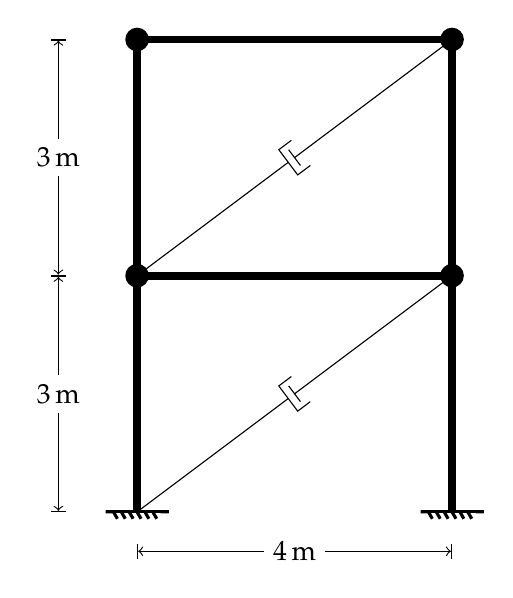
\begin{tikzpicture}
\draw[|<->|](0,-.5)--(4,-.5)node[midway,fill=white]{\SI{4}{\meter}};
\draw[|<->|](-1,0)--(-1,3)node[midway,fill=white]{\SI{3}{\meter}};
\draw[|<->|](-1,3)--(-1,6)node[midway,fill=white]{\SI{3}{\meter}};
\FixedSupport{0,0}
\FixedSupport{4,0}
\draw[line width=1mm](0,0)--(0,6)node[fill=black,circle,inner sep=0,minimum size=3mm]{}--(4,6)node[fill=black,circle,inner sep=0,minimum size=3mm]{}--(4,0);
\draw[line width=1mm](0,3)node[fill=black,circle,inner sep=0,minimum size=3mm]{}--(4,3)node[fill=black,circle,inner sep=0,minimum size=3mm]{};
\begin{scope}[rotate=36.8699]
\draw(0,0)--(2.4,0)(2.6,.2)--(2.4,.2)--(2.4,-.2)--(2.6,-.2)(2.5,.125)--(2.5,-.125)(2.5,0)--(5,0);
\end{scope}
\begin{scope}[rotate around={36.8699:(0,3)}]
\draw(0,0+3)--(2.4,0+3)(2.6,.2+3)--(2.4,.2+3)--(2.4,-.2+3)--(2.6,-.2+3)(2.5,.125+3)--(2.5,-.125+3)(2.5,0+3)--(5,0+3);
\end{scope}
\end{tikzpicture}
\end{document}